\newcommand{\CTAN}[1]{\textsl{#1}}

\chapter{Mode d'emploi}
%\localtableofcontents{}

\section{Avertissements}

{\huge\color{red}
\begin{enumerate}
\item Élaboration en cours
  \begin{itemize}
  \item Temporairement, des incompatibilité de packages peuvent être présentes
  \end{itemize}
\item Pas de rétro-compatibilité assurée!
  \begin{itemize}
  \item Faire une sauvegarde ou copie avant de procéder à une mise à jour de la fourniture \UGE.
  \end{itemize}
\end{enumerate}
}

\section{En cas de problèmes}

\begin{Attention}{Conflit avec installation locale}
  \begin{itemize}
  \item Bien vérifier qu'il n'y pas conflit avec des installations locales la/tex  (\~/texmf)!
  \item Les fichiers chargés sont effectivement les fichiers prévus et non pas des copies résiduelles enregistrées localement (et potentiellement obsolètes).
  \end{itemize}
\end{Attention}


\begin{itemize}
\item Recompiler plusieurs fois si nécessaire!
\end{itemize}

\subsection{Overleaf}
\begin{itemize}
\item \url{}
\end{itemize}

\subsection{Chat univ-eiffel.fr}

\begin{itemize}
\item \url{https://chat.univ-eiffel.fr} / \verb|LaTeX&Overleaf@UGE|

\item \url{https://go.rocket.chat/invite?host=chat.univ-eiffel.fr\&path=invite\%2Fkc6eCm}
\end{itemize}
\subsection{Messagerie}

\begin{itemize}
\item \url{mailto://jorge.mariano@univ-eiffel.fr}
\end{itemize}

\section{Structuration}
\label{sec:structuration}


\paragraph{NB}

\begin{itemize}
\item Le document est «déposé» dans le sous-répertoire .src.

\item Les éléments dont le nom est préfixé par UGE ne sont pas destinés à être modifiés par l'utilisateur. Cela reste évidemment techniquement possible...
\end{itemize}

Pour faciliter la maintenance, la mise au point, la structuration proposée permet de décomposer facilement le travail selon divers usages :
\begin{itemize}
\item génération totale ou partielle, avec ou sans le modèle UGE.
\end{itemize}



\subsection{Éléments du modèle UGE}

Les différents éléments constituifs du modèle glonal sont actuellement séparés, pour faciliter la mise au point et la réutilisation partielle.

\newcommand{\UGEtext}[1]{%
  {\color{#1} \textbf{Couleur #1}}
}

\paragraph{UGE-Col.sty}

\begin{itemize}
\item Les 11 couleurs spécifiées dans la charte UGE sont définies en valeurs (R,G,B)
\item Les couleurs standard LaTeX bleu, noir, cyan, pink, purple, orange, green, et red sont redéfinies via les couleurs UGE. Il n'est pas nécessaire d'utiliser les noms UGE pour les couleurs de cette liste.
\end{itemize}

  \begin{minipage}[t]{.45\linewidth}  
    \begin{enumerate}
    \item \UGEtext{UGEcolBlue}
    \item \UGEtext{UGEcolBlueLight}
    \item \UGEtext{UGEcolBlack}
    \item \UGEtext{UGEcolCyan}
    \item \UGEtext{UGEcolPink}
    \item \UGEtext{UGEcolPurple}
    \item \UGEtext{UGEcolOrange}
    \item \UGEtext{UGEcolOrangeLight}
    \item \UGEtext{UGEcolGreen}
    \item \UGEtext{UGEcolGreenLight}
    \item \UGEtext{UGEcolRed}
    \end{enumerate}
  \end{minipage}
  \begin{minipage}[t]{.45\linewidth}  
    \begin{enumerate}
    \item \UGEtext{blue} 
    \item 
    \item \UGEtext{black} 
    \item \UGEtext{cyan} 
    \item \UGEtext{pink} 
    \item \UGEtext{purple}
    \item \UGEtext{orange}
    \item 
    \item 
    \item \UGEtext{green} 
    \item \UGEtext{red} 
    \end{enumerate}
  \end{minipage}


  \paragraph{UGE-Fontes.sty}
  \begin{itemize}
  \item Sélection des polices de caractère, notamment TT-Norms (charte UGE) si disponible, sinon une autre police plus courante (à définir) est sélectionnée.
  \end{itemize}
  
  \paragraph{UGE-Thesis-FP.sty}
\begin{itemize}
\item Première page de thèse UGE (logos, identification de la thèse, du doctorant)
\end{itemize}

  \paragraph{UGE-Bib.sty}
\begin{itemize}
\item Paramétrage biblatex
\end{itemize}

\paragraph{UGE-Template.sty}
\begin{itemize}
\item Ensemble des packages et macros spécifique à la restitution graphique UGE
\end{itemize}

\paragraph{doc-form.tex}
\begin{itemize}
\item Informations caractéristiques du document (auteur, titre, \ldots{})
\end{itemize}

\paragraph{jury.tex}
\begin{itemize}
\item Pour une thèse, constitution du jury. Intégré dans la première page.
\end{itemize}

\paragraph{UGE-Notes.tex}
\begin{itemize}
\item Documentation (en cours) d'utilisation et technique du modèle UGE.
\end{itemize}

\subsection{Éléments du document}

\paragraph{.src/}

\begin{itemize}
\item Sous-dossier contenant l'intégralité du document utilisateur à générer
\end{itemize}

\paragraph{.src/body.tex}

\begin{itemize}
\item Fichier maître pour le document utilisateur. Il intègre les autres fichiers nécessaires.
\end{itemize}

\paragraph{Ch-NN.tex}

\begin{itemize}
\item les différents chapitres
\item intégrés via include pour profiter de la compilation conditionnelle (includeonly)
\end{itemize}

\subsection{Auxiliaires}

\paragraph{JMR.sty}

\begin{itemize}
\item Sélection de packages et macros généralement utiles et/ou recommandés pour la production de documents LaTeX
\end{itemize}

\paragraph{local.sty}

\begin{itemize}
\item Packages et macros strictement nécessaires à la compilation du document sans utilisation du modèle \UGE.
  Permet d'identifier les besoins techniques du document indépendamment du contexte \UGE.
\end{itemize}

\paragraph{latexmkrc.00}

\begin{itemize}
\item Modèle pour le fichier de configuration latexmkrc
\end{itemize}


\paragraph{minimal.tex}

\begin{itemize}
\item Pour compiler le document (.src/body.tex) SANS activer le modèle UGE.
\end{itemize}


\subsection{Organisation générale}

\begin{figure}
  \centering
  \fbox{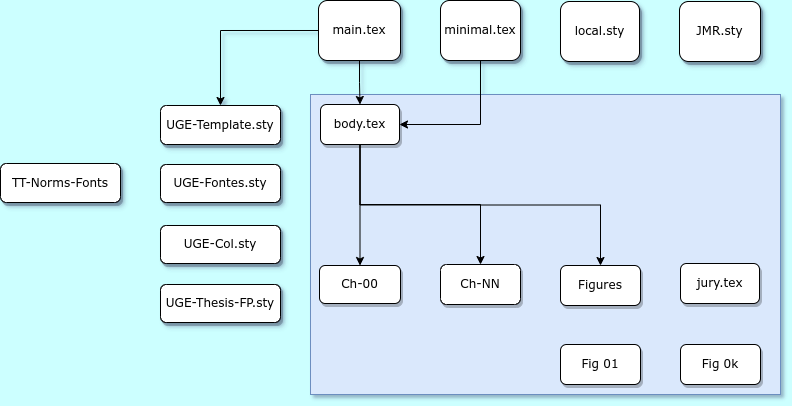
\includegraphics[width=\columnwidth]{UGE-Template.drawio.png}}
  \caption{Organisation générale des fichiers}
\end{figure}

\section{Usage}

\subsection{Includeonly}


\centering\begin{boxedminipage}{.5\columnwidth}\small
\begin{verbatim}
\documentclass{book}

%% PREAMBLE!
\includeonly{file-01}
...
%\includeonly{file-0n}
%%
\begin{document}
\include{file-01}
...
\include{file-0n}
\end{document}

\end{verbatim}
    
  \end{boxedminipage}

\subsection{Première page}

\begin{itemize}
\item La première page est spécifiée dans UGE-Thesis-FP
\end{itemize}
\subsection{LaTeXmk}

\begin{itemize}
\item Contrôle du processus de compilation du document
\item C'est le même outil que celui utilisé par Overleaf
  \begin{itemize}
  \item Le template UGE doit/peut donc être complètement compatible Overleaf
  \end{itemize}
\end{itemize}

\paragraph{Commandes usuelles}

\begin{itemize}
\item \texttt{latexmk main}, compilation générale avec modèle UGE
\item \texttt{latexmk minimal} compilation générale sans modèle
\item \texttt{latexmk -C minimal} nettoyage des fichiers intermédiaires facultatifs
\end{itemize}


\paragraph{NB}

Si latexmkrc est correctement configuré, (le fichier par défaut est alors défini comme \texttt{main.tex})
\begin{itemize}
\item la génération du document se fait simplement via \texttt{latexmk}
\item le nettoyage du dossier se fait simplement via \texttt{latexmk -C}
\item donc pour une compilation «totale» (plus longue) : \texttt{latexmk -C ; latexmk}
\end{itemize}


\subsection{LuaLaTeX}

\begin{itemize}
\item
\end{itemize}



\section{Technique}

\subsection{Fonctionnalités}

Intégrées dans la proposition actuelle de  «template»

\begin{description}
\item[Charte UGE]
  \begin{itemize}
  \item Définition des couleurs via \CTAN{xcolor}
  \end{itemize}
\item[Bibliographie]
  \begin{itemize}
  \item \CTAN{Biblatex}/\CTAN{biber}
  \end{itemize}
\item[Fontes et polices]
  \begin{itemize}
 \item Fonte de caractère charte  UGE
\item Ligatures artistiques facultatives
\item Chargement local des fontes TTF
  \end{itemize}
\item[Structuration, génération]
  \begin{itemize}
 \item Utilisation latexmkrc / cf Overleaf
  \item Compilation partielle includeonly
  \end{itemize}
\item[Sectionnements]
  \begin{itemize}
  \item Parties / Numérotation littérale française (première, deuxième,...)
  \item Troncature des entêtes via \CTAN{troncate}
  \end{itemize}
\item[Table des matières]
  \begin{itemize}
  \item Tables locales par chapitre
  \item Saut de page avant le corps du chapitre
  \end{itemize}
\item[Divers/Debug]
  \begin{itemize}
  \item \item Watermark
  \item Debug labels \CTAN{showlabels}
  \item Affichage coloré des lignes avec défauts typographiques (lualatex/\CTAN{lua-typo})
  \end{itemize}
\end{description}

Le modèle UGE met en oeuvre les techniques disponibles les plus récentes et recommandées.

Ainsi, plusieurs remplacements sont nécessaires :

\begin{enumerate}
\item LuaLaTeX remplace LaTeX
\item BibLaTeX remplace BibTeX
\item etoc remplace minitoc
\end{enumerate}

Ou des choix de solutions techniques sont effectués :
\begin{itemize}
\item latexmk (.latexmkrc), pour le processus de compilation, génération du document
\item fontspec pour la sélection simple des polices/fontes (TTF, OTF)
\end{itemize}

\subsection{Sur la pile }

Extensions probablement utiles à intégrer :

\begin{itemize}
\item \CTAN{microtype}
\end{itemize}

\section{Notes sur le codage}

\begin{itemize}
\item Ne pas utiliser le double slash pour marquer un changement de paragraph
\item Ne pas utiliser bigskip pour corriger les espacements verticaux de sections
  \begin{itemize}
  \item Adapter le style de sections
  \end{itemize}
\item Ne pas donner de label numériques (1.2.3)
  \begin{itemize}
  \item Les labels sont symboliques (intro-section, probleme-annexe, ...)
  \end{itemize}
\item Attention à l'encodage des fichers .tex (doit être UTF8)
\item Ne pas spécifier les extensions de type pour les fichiers graphiques (sauf besoin spécifique identifié)
\end{itemize}

\paragraph{Test}

Passer le document

\begin{itemize}
\item Orientation paysage (landscape) et non portrait
\item Misen forme sur deux colonnes
\end{itemize}

\begin{verbatim}
\documentclass[...,landscape,twocolumn]{book}
\begin{document}
\twocolumn
.
% Préambule
\pagestyle{fancy}

%% ______________________________ %%
% READING GUIDE
%------------------------------%
%% ✎ Dylan (V1) %%%%%%%%% ✅ %%
%% ✎ Alain (V2) %%%%%%%%% ✅ %%
%% ✎ Dylan (V3) %%%%%%%%% ✅ %%
%------------------------------%

%\cleardoublepage
    \needspace{1\baselineskip} % Reserve space
\chapter*{Reading Guide of the Manuscript
    \label{body:guide-lecture-manuscrit}
    }
    \markboth{Reading Guide of the Manuscript}{}
    \markright{Preface}{}
    \addcontentsline{toc}{part}{Reading Guide of the Manuscript}

% --- %
    % Ecriture inclusive
% \section*{Adoption de l'écriture inclusive
%     \label{subbody:adoption-ecriture-inclusive}
%     }
%     \addcontentsline{toc}{section}{Adoption de l'écriture inclusive}

% \lettrine[lines=3, findent=8pt, nindent=0pt]{\lettrinefont A}{dopter} une approche d'écriture inclusive vise à promouvoir une représentation équilibrée des genres dans la langue écrite, afin de lutter contre les stéréotypes de genre tout en mettant en valeur la diversité des personnes. L'écriture inclusive ne prétend pas complexifier la langue, mais plutôt rendre l'écriture plus représentative de la réalité sociale en nous invitant à repenser notre façon de communiquer. Au lieu d'alourdir la lecture, l'écriture inclusive offre bien au contraire des tournures grammaticales plus fluides et concises. D'après le manuel d'écriture inclusive publié par \textcolor{blue}{Raphaël} \textcolor{blue}{\textcite[19-23]{haddad_manuel_2019}}\index{Haddad, Raphaël|pagebf}, l'écriture inclusive permet de déconstruire dix arguments majeurs: (i) elle n'aurait pas d'influence sur nos représentations; (ii) serait trop compliquée à utiliser; (iii) encombrerait, et même (iv) défigurerait le texte; (v) elle serait interdite par certaines institutions, (vi) car elle menacerait la langue française, (vii) en promouvant la \textsl{novlangue}, (viii) et en ayant des règles hétérogènes; (ix) tandis que le masculin serait le marqueur du neutre, (x) et qu'il serait signe de prestige en français.%%Rédigé%%

% À cet égard, nous avons fait le choix d'inclure le point médian (·) qui intègre à la fois la forme féminine et masculine. Conscient·e·s que cette démarche nécessite un temps d'adaptation, nous avons fait le choix d'énumérer les quelques mots spécifiquement affectés par l'adoption de l'écriture inclusive afin de guider la lecture pour tou·te·s.%%Rédigé%%

% --- %
    % Types of Scientific Productions
    \needspace{1\baselineskip} % Reserve space
\section*{Nomenclature of Scientific Productions
    \label{subbody:nomenclature-productions-scientifiques}
    }
    \addcontentsline{toc}{section}{Nomenclature of Scientific Productions in Human and Social Sciences}

\acrfull{Hcéres} has established, in France, a nomenclature for scientific productions in \acrfull{HSS}. This framework aims to categorize the different types of scientific outputs produced by researchers, in the context of evaluating research institutions. The proposed coding is present throughout the doctoral thesis, within the sections listing scientific productions related to each chapter. The nomenclature is as follows \textcolor{blue}{\autocite{ministere_de_leducation_nationale_de_lenseignement_superieur_et_de_la_recherche_nomenclatures_nodate}}\index{Ministère de l'Éducation Nationale, de l'Enseignement Supérieur et de la Recherche@\textsl{Ministère de l'Éducation Nationale, de l'Enseignement Supérieur et de la Recherche}|pagebf}:%%Translated%%

    \needspace{1\baselineskip} % Reserve space
\subsubsection*{Scientific Publications:}
    \begin{customitemize}
\item \textbf{ACL}: Articles in international or national peer-reviewed journals listed by \acrshort{Hcéres} or in international databases;
\item \textbf{ACLN}: Articles in peer-reviewed journals not listed by \acrshort{Hcéres} or in international databases;
\item \textbf{ASCL}: Articles in journals without peer review;
\item \textbf{OS}: Scientific books (including critical editions and scientific translations);
\item \textbf{PT}: Transfer publications.
    \end{customitemize}

    \needspace{1\baselineskip} % Reserve space
\subsubsection*{Scientific Events:}
    \begin{customitemize}
\item \textbf{C-INV}: Keynote lectures given at the invitation of the Organizing Committee at a national or international conference;
\item \textbf{C-ACTI}: Presentations with proceedings at an international conference;
\item \textbf{C-ACTN}: Presentations with proceedings at a national conference;
\item \textbf{C-COM}: Oral presentations without proceedings at a national or international conference;
\item \textbf{C-AFF}: Poster presentations at a national or international conference.
    \end{customitemize}

    \needspace{1\baselineskip} % Reserve space
\subsubsection*{Dissemination of Scientific Culture:}
    \begin{customitemize}
\item \textbf{PV}: Popular science publications;
\item \textbf{PAT}: Theorized artistic productions.
    \end{customitemize}

    \needspace{1\baselineskip} % Reserve space
\subsubsection*{Other Productions:}
    \begin{customitemize}
\item \textbf{BRE}: Patents;
\item \textbf{DO}: Editorial direction of books or journals;
\item \textbf{OR}: Research tools;
\item \textbf{TH}: Doctoral theses;
\item \textbf{AP}: Other productions.
    \end{customitemize}

% --- %
    % LaTeX
    \needspace{1\baselineskip} % Reserve space
\section*{The Benefits of \latexword{\LaTeX} in \acrlong{HSS}
    \label{subbody:interet-latex}
    }
    \addcontentsline{toc}{section}{The Benefits of \latexword{\LaTeX} in Human and Social Sciences}

    % Writing in LaTeX
\lettrine[lines=3, findent=8pt, nindent=0pt]{\lettrinefont I}{n} closing this section dedicated to the reading recommendations of this manuscript, it is appropriate to inform the reader that this doctoral thesis has been written using the document preparation system \latexword{\LaTeX}. The decision to opt for this computer language, known as \Commas{light markup}, or \textsl{balisage léger} \textcolor{blue}{\autocite[16]{pochet_markdown_2023}}\index{Pochet, Bernard|pagebf}, should not remain unexplained, as a brief outline of its advantages may, we hope, encourage its adoption in our disciplines. Indeed, the use of \latexword{\LaTeX}, far beyond a mere stylistic preference, aligns with a commitment to academic excellence and the renewal of research practices. However, although \latexword{\LaTeX}-written books are widespread, few are specifically dedicated to \acrshort{HSS} \textcolor{blue}{\autocite[7]{rouquette_xelatex_2012}}\index{Rouquette, Maïeul|pagebf}.%%Translated%%

    % Advantages of LaTeX
Building on the argumentation developed by \textcolor{blue}{\textcite[8-9]{rouquette_xelatex_2012}}\index{Rouquette, Maïeul|pagebf} in his work titled \textsl{(Xe)LaTeX Applied to the Humanities} (\textsl{(Xe)LaTeX appliqué aux sciences humaines}), it appears that \acrfull{WYSIWYG} software, such as \Marque{Microsoft Office Word}\footnote{
    \Marque{Microsoft Office Word} (\url{https://www.microsoft.com/fr-fr/microsoft-365/word}) is a word processing software, distributed since 1983 and is now part of the \textsl{Microsoft Office} suite.
} or \Marque{LibreOffice}\footnote{
    \Marque{LibreOffice} (\url{https://www.libreoffice.org/}) is a free and open-source office suite, developed by the non-profit organization \Marque{Document Foundation}.
}, face various challenges in word processing, especially for long documents. In contrast, the \latexword{\LaTeX} system and language stand out for their typographic precision, facilitating the management of large documents and the handling of bibliographic references. The separation between the text editor and the compiler in \latexword{\LaTeX} allows for a clear distinction between content and formatting, with the document being produced in an open PDF format (\textsl{Portable Document Format}). From our perspective, the use of \latexword{\LaTeX} is justified by numerous advantages in the context of our doctoral research:
    \begin{customitemize}
\item Reproducibility and longevity of the manuscript, independent of software evolution;
\item Free and open-source computer language, reliable for over three decades, compatible with all operating systems;
\item Easy access via the PDF format;
\item Optimized management and time-saving for long documents, such as a doctoral thesis;
\item Compliance with academic publisher standards, who favor this format for scientific publications;
\item Collaborative nature facilitated by an online text editor such as \Marque{Overleaf}, which offers proofreading and commenting features\footnote{
    \Marque{Overleaf} (\url{https://www.overleaf.com/}) is a \latexword{\LaTeX} editor that combines a code editor with a preview, while enabling real-time collaboration with sharing and versioning features. The online platform integrates reference management software like \Marque{Zotero} and \Marque{Mendeley}.
};
\item Recognition of professional typography due to full support for typographic rules;
\item Simplified management of bibliographies and mathematical formulas;
\item Advanced customization through commands, enhanced by additional modules (\textsl{packages});
\item Ability to include content and annotations not visible in the final output;
\item Support and contribution from a particularly active \latexword{\LaTeX} community.
    \end{customitemize}%%Translated%%

    % Acknowledgements LaTeX
From a more personal perspective, I would like to express my deep gratitude to \textcolor{blue}{Jorge Mariano}\index{Mariano, Jorge|pagebf}, Research Engineer at Gustave Eiffel University, for his significant contribution to the design of a \latexword{\LaTeX} template that meets the visual standards of Gustave Eiffel University, as well as for his ongoing support. This manuscript partially incorporates this template and has been enhanced with modifications aimed at better customization for the specific needs of our discipline and our individual preferences. The adoption of \latexword{\LaTeX} was also made possible thanks to the valuable advice of my thesis supervisor, \textcolor{blue}{Alain L'Hostis}\index{L'Hostis, Alain|pagebf}, who, from the beginning of my doctoral journey, convinced me of the merits of this system and programming language. My thoughts go to my colleague and friend \textcolor{blue}{Iñigo Aguas Ardaiz}\index{Aguas Ardaiz, Iñigo|pagebf}, who, at the end of my research, generously gave me his precious time and provided invaluable help in resolving the code issues. Finally, I would like to thank Gustave Eiffel University for supporting my professional access to the \latexword{\LaTeX} collaboration environment \Marque{Overleaf}.%%Translated%%

    % GitHub Link
With the aim of open science and, consequently, the sharing of knowledge, reuse, and collaboration, we have made this manuscript, along with the customized template and code used, accessible through a \Marque{GitHub} repository\footnote{
    \Marque{GitHub} (\url{https://github.com/}) is an online platform for software development management and a hosting service for open access projects.
}.%%Translated%%

    \bigskip
    \begin{tcolorbox}[colback=white!5!white,
                      colframe=blue!75!blue,
                      title=
                      \bigskip
                      \center{\Marque{GitHub} Repository}
                      \bigskip]
\center{\normalsize{\url{https://github.com/dylan-moinse/PhD_Thesis_Dylan_MOINSE_English}}}
    \end{tcolorbox}

%% ______________________________ %%
% ACKNOWLEDGEMENTS
%------------------------------%
%% ✎ Dylan (V1) %%%%%%%%% ✅ %%
%% ✎ Alain (V2) %%%%%%%%% ✅ %%
%% ✎ Dylan (V3) %%%%%%%%% ✅ %%
%------------------------------%

% ACKNOWLEDGEMENTS
    \cleardoublepage
    \needspace{1\baselineskip} % Reserve space
\chapter*{Acknowledgements
    \label{body:remerciements}
    }
    \markboth{Acknowledgements}{}
    \markright{Preface}{}
    \addcontentsline{toc}{part}{Acknowledgements}

    % Introduction
\lettrine[lines=3, findent=8pt, nindent=0pt]{\lettrinefont W}{elcome} aboard this \textsl{collective} work. This adjective, in my eyes, best describes the genesis of this doctoral research, the result of four or five years – the exact count still escapes me – of shared labor. Similar to the construction of a house, however modest it may be in the urban landscape, this manuscript is the realization of the investment of many hands. This doctoral thesis, encompassing the manuscript and the scientific productions that stem from it, was made possible thanks to the contribution of many knowledge artisans. To these collaborators, true builders both intellectually and emotionally, to whom I wish to pay tribute, I fear I cannot name all of them within the limited space of these few pages. Nevertheless, I engage in this exercise of recognition, for which words alone would not suffice to fully express my gratitude. In this spirit, mindful of not being able to fully communicate my esteem for your support and daily efforts, I have chosen to materialize these acknowledgements in the form of a map (see the \hyperref[fig-introduction:remerciements]{Acknowledgement Map}, page~\pageref{fig-introduction:remerciements}). The first, but certainly not the last in this document, rest assured.%%Translated%%

    % Supervision
There can be no \textsl{correct} order to mention all the people who contributed to enriching this doctoral experience. However, I must first and foremost express my deepest gratitude to \textcolor{blue}{Alain L'Hostis}, who has exercised his responsibilities as thesis supervisor with constant kindness and good humor. His qualities, both scientific and human, have been an invaluable source of inspiration and encouragement throughout this journey. From my research internship, he welcomed me under the best conditions. I am deeply grateful to him for his availability, and especially for the trust and great freedom he granted me in guiding this project. This trust honors me, and I hope that this thesis, in its own way, manages to repay a part of what has been so generously given to me.%%Translated%%

    % CSI and Jury
I also wish to express my gratitude to \textcolor{blue}{Laurent Chapelon} and \textcolor{blue}{Chia-Lin Chen}, who evaluated this doctoral thesis as \textsl{rapporteurs}, as well as to \textcolor{blue}{Ahad Amini Pishro}, \textcolor{blue}{Sophie Hasiak}, and \textcolor{blue}{Patrick Rérat}, who agreed to be part of the jury. Furthermore, I extend my thanks to \textcolor{blue}{Marc Dumont} and \textcolor{blue}{Vaclav Stransky}, who generously accepted to follow the progress of my doctoral research. Lastly, my gratitude goes to \textcolor{blue}{Philippe Menerault}, whose teachings during my academic journey inspired me. His wise advice has been of invaluable help.%%Translated%%

    % Institutions
I am aware of the extremely favorable conditions under which my research was carried out, both in terms of financial support and scientific guidance. More broadly, I recognize the privilege of having worked in such a rich professional environment, both in Lille and in Paris, as part of a laboratory driven by such passionate and caring individuals. I owe this pleasant atmosphere largely to the support of Gustave Eiffel University and the Hauts-de-France Region, through the \textsl{rev3} program, which financed this research project.%%Translated%%

    % Support
\textsl{Last but not least}, it is impossible for me to continue writing this section dedicated to acknowledgements without mentioning my family, to whom I dedicate this manuscript. You are my role model, and I am committed to honoring the tenacity and ethical values you have passed on to me. To everyone I hold dear.%%Translated%%

    % Acknowledgement Map
    \begin{carte}[h!]\vspace*{4pt}
        \caption*{Acknowledgement Map}
        \label{fig-introduction:remerciements}
        \centerline{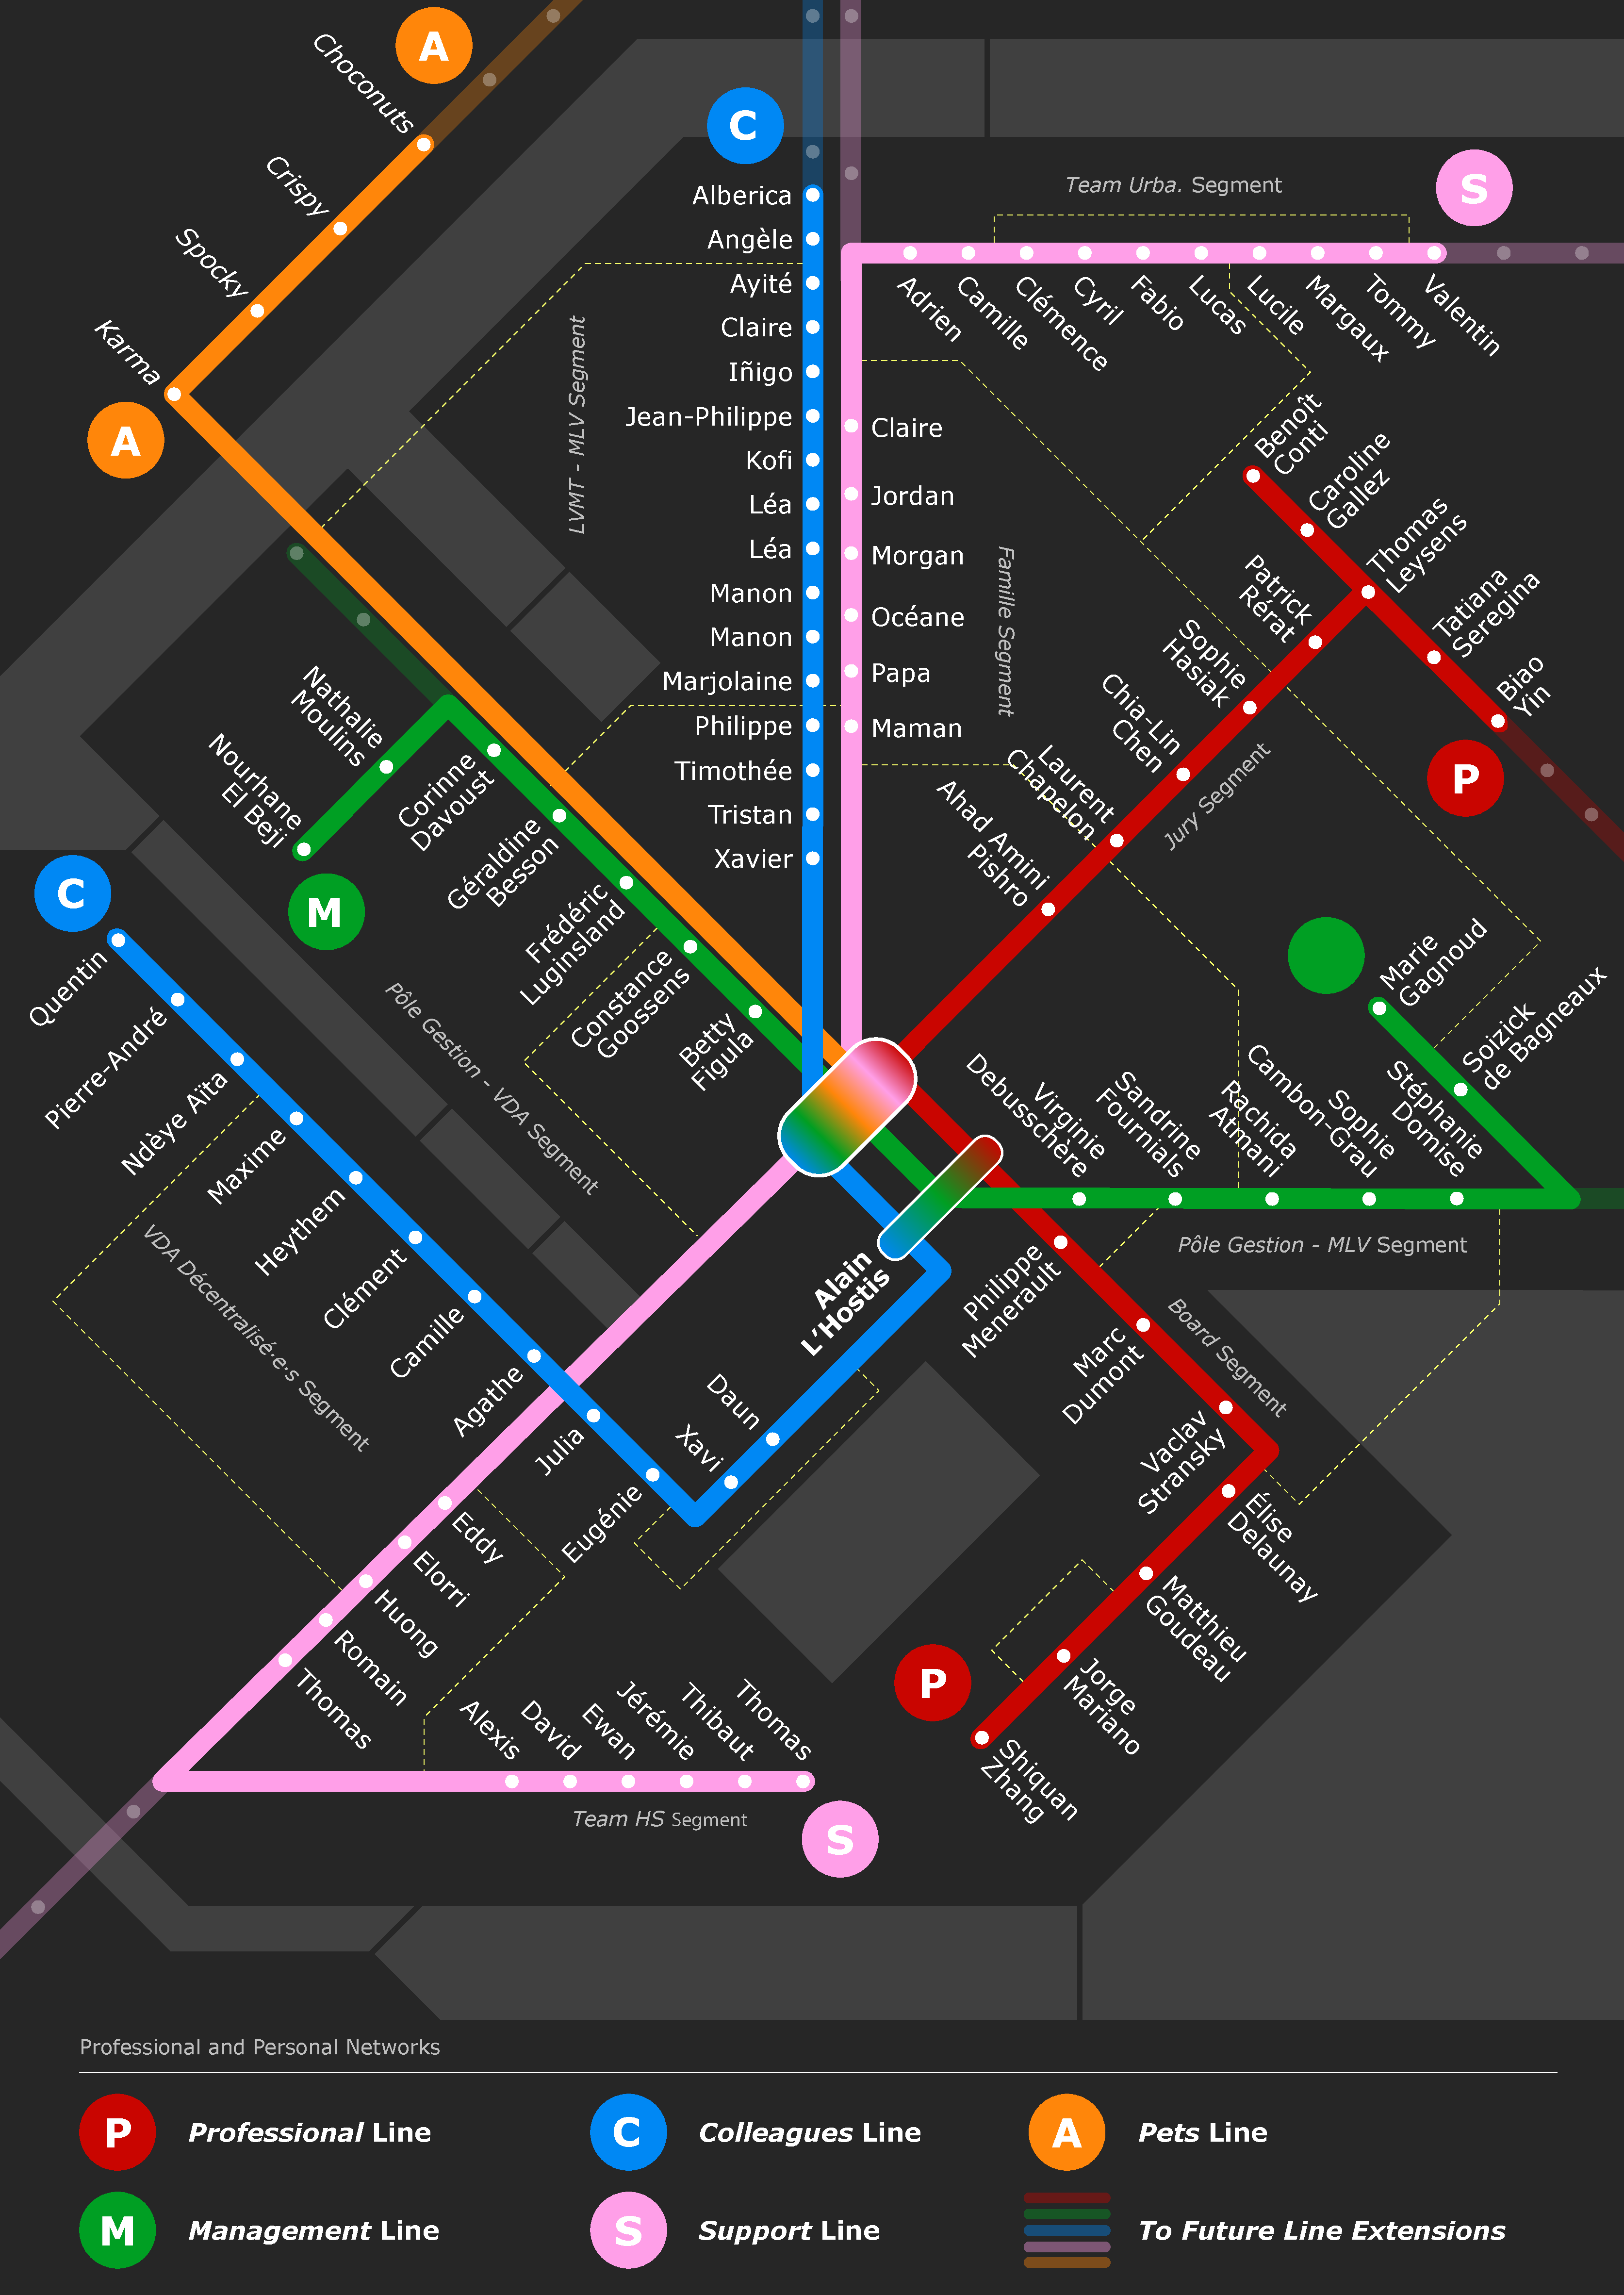
\includegraphics[width=1\columnwidth]{src/Figures/Preambule/EN_Remerciements.pdf}}
        \vspace{5pt}
        \begin{flushright}\scriptsize{
        Author: \textcolor{blue}{Dylan Moinse (2024)}
        }\end{flushright}
    \end{carte}

%% ______________________________ %%
% TOC
    \cleardoublepage
    \setcounter{tocdepth}{1}
\tableofcontents{}
    \markboth{Table of Contents}{}
    \markright{Preface}{}
    %\addcontentsline{toc}{part}{Table des matières}
    \noindent\makebox[\textwidth]{\hrulefill}

%% ______________________________ %%
% LIST FIGURES
\listof{figure}{List of Figures}
    \markboth{List of Figures}{}
    \markright{Preface}{}
    \addcontentsline{toc}{part}{List of Figures}
    \noindent\makebox[\textwidth]{\hrulefill}

%% ______________________________ %%
% LIST MAPS
\listof{carte}{List of Maps}
    \markboth{List of Maps}{}
    \markright{Preface}{}
    \addcontentsline{toc}{part}{List of Maps}
    \noindent\makebox[\textwidth]{\hrulefill}

%% ______________________________ %%
% LIST TABLES
\listof{table}{List of Tables}
    \markboth{List of Tables}{}
    \markright{Preface}{}
    \addcontentsline{toc}{part}{List of Tables}
    \noindent\makebox[\textwidth]{\hrulefill}

%% ______________________________ %%
% QUOTE DOCUMENT
%------------------------------%
%% ✎ Dylan (V1) %%%%%%%%% ✅ %%
%% ✎ Alain (V2) %%%%%%%%% ✅ %%
%% ✎ Dylan (V3) %%%%%%%%% ✅ %%
%------------------------------%

\cleardoublepage
\section*{Citing the Document
    \label{body:citer-document}
    }
    \addcontentsline{toc}{part}{Citing the Document}
    \markboth{Citing the Document}{}
    \markright{Preface}{}

\small{\textcolor{blue}{Moinse Dylan (2025)}, \textsl{The Transit-Oriented Development Urban Model Revisited by Emerging Light Individual Mobility. An Investigation in the Hauts-de-France Region} (Doctoral Thesis in Spatial Planning, Urbanism). Gustave Eiffel University, Laboratoire Ville Mobilité Transport. Supervised by \textcolor{blue}{L'Hostis Alain}, \pageref{LastPage}~p.}

%% ______________________________ %%
% FOREWORD
%------------------------------%
%% ✎ Dylan (V1) %%%%%%%%% ✅ %%
%% ✎ Alain (V2) %%%%%%%%% ✅ %%
%% ✎ Dylan (V3) %%%%%%%%% ✅ %%
%------------------------------%

\cleardoublepage
\section*{Foreword
    \label{body:avant-propos}
    }
    \addcontentsline{toc}{part}{Foreword}
    \markboth{Foreword}{}
    \markright{Preface}{}

    % Figure logo HdF
\begin{wrapfigure}[6]{r}{0.2\textwidth} % 6 lignes pour ajuster la hauteur
    \vspace{-10pt} % Réduit l'espacement vertical avant la figure
    
\includegraphics[width=\linewidth]{src/Figures/Introduction/Logo_HdF.jpg} 
    \caption*{}
    \label{fig-introduction:logo-hdf}
\end{wrapfigure}

    % Introduction
This doctoral research was conducted at Gustave Eiffel University\footnote{
    Gustave Eiffel University is an \acrfull{EPSCP}, founded in 2020 \textcolor{blue}{\autocite{universite_gustave_eiffel_notre_2024}}\index{Université Gustave Eiffel@\textsl{Université Gustave Eiffel}|pagebf}. It resulted from the merger and consolidation of a university, a research organization, and several schools, including notably \acrfull{IFSTTAR}, \acrfull{UPEM}, and other associated institutions.
}, within the \acrfull{LVMT}\footnote{
    The \acrfull{LVMT} is a \acrfull{UMR} founded in 2003, under the joint supervision of Gustave Eiffel University and the Institut Polytechnique de Paris, the latter being formed from a merger that notably included \acrfull{ENPC}. The \acrshort{LVMT} focuses on the study of the interactions between territories, transport, and mobility, utilizing multidisciplinary approaches from urban planning, geography, economics, sociology, anthropology, and engineering sciences \textcolor{blue}{\autocite{laboratoire_ville_mobilite_transport_presentation_2024}}\index{Laboratoire Ville Mobilité Transport@\textsl{Laboratoire Ville Mobilité Transport}|pagebf}.
}. The doctoral contract was co-financed by the Hauts-de-France Region, within the framework of the \textsl{rev3} initiative (\textsl{Third Industrial Revolution})\footnote{
    The \textsl{rev3} initiative (\textsl{Third Industrial Revolution}) is a collective dynamic launched in 2013, co-led by the Hauts-de-France Region and the \acrfull{CCI} Hauts-de-France. It aims to design and promote innovative territorial development models, set within a sustainable perspective towards 2050 \textcolor{blue}{\autocite{rev3_rev3_2022}}\index{rev3@\textsl{rev3}|pagebf}.
}. This doctoral thesis aligns with the second \acrfull{COP} 2023-2025 of Gustave Eiffel University\footnote{
    It particularly aligns with Strategic Project~2.1 (\Commas{Developing decarbonized mobility for all users and across all territories safely, based on the understanding of mobility behaviors and usage}) and~2.4 (\Commas{Progressing in development models integrating the Sustainable Development Goals}).
} and with the third research axis \Commas{Urban Planning and Territories}\footnote{
    Axis~3 \Commas{Urban Planning and Territories} of the \acrfull{LVMT} focuses on the study of interactions between territories, transport, and mobility \textcolor{blue}{\autocite{laboratoire_ville_mobilite_transport_axe_2024}}\index{Laboratoire Ville Mobilité Transport@\textsl{Laboratoire Ville Mobilité Transport}|pagebf}. It explores territorial dynamics and their modeling, transport network connections, urban planning models, and energy efficiency challenges. Research in this field revolves around two main levels of interaction. On one hand, it examines transport hubs, analyzing the flows they polarize, the developments they generate, and their strategic role for public and private actors. On the other hand, it studies how transport networks contribute to strengthening the links between territories, while influencing urban forms and relationships within regional urban systems.
} of the \acrshort{LVMT}.%%Translated%%


%% ______________________________ %%
% CAPTATIO BENEVOLENTIAE
%------------------------------%
%% ✎ Dylan (V1) %%%%%%%%% ✅ %%
%% ✎ Alain (V2) %%%%%%%%% ✅ %%
%% ✎ Dylan (V3) %%%%%%%%% ✅ %%
%------------------------------%

\cleardoublepage
\section*{\textsl{Captatio benevolentiae}
    \label{body:mt180}
    }
    \addcontentsline{toc}{part}{\textsl{Captatio benevolentiae}}
    \markboth{\textsl{Captatio benevolentiae}}{}
    \markright{Preface}{}

%\poemtitle{Before Automobility, the Quest for Intermodality}
\subsection*{Before Automobility, the Quest for Intermodality (\textsl{Devant l'Automobilité, la quête de l'Intermodalité}}
    
\settowidth{\versewidth}{And objects at rest tended to remain at rest}
\begin{verse}[\versewidth]

Il était une fois,\\
Au cœur du lointain eldorado lillois,\\
Une splendide Princesse appelée \textsl{Pieds}\\
Épousa le Prince \textsl{Train}, en un lien sacré et privilégié.\\
Cette union vénérée régnait sur la nation,\\
Organisée par des zones piétonnes et des stations.

Or, brusquement, cette relation idyllique\\
Fut renversée par une rivale maléfique.\\
La sorcière \textsl{La Voiture} insuffla un sortilège,\\
Envoûtant ces terres de mille pièges.\\
Le pays se pervertit en périphéries éparpillées.\\
Aux paysages pollués et aux chemins embouteillés.

Afin de briser l’envoûtement de \textsl{La Voiture},\\
Le pouvoir valorisa les gares sans véritable rupture.\\
En vain, les individus véhiculés vivant loin.

Pris de panique, \textsl{Pieds} et \textsl{Train} appelèrent leurs adjoints,\\
Les fidèles \textsl{Bus}, \textsl{Tramway} et \textsl{Métropolitain},\\
Hélas, peu adaptés à l’espace dépeint, rendant l'effort vain.

Las de ces lieux esclaves des lois de l’automobile,\\
Les nobles se tournèrent vers \textsl{Vélo}, un chevalier habile.\\
Surnommé \textsl{La Petite Reine} après son arrivée,\\
\textsl{Vélo} a pour vertu d'étendre les périmètres des gares fortifiées.

Mais, l’énergie conquérante de \textsl{Vélo} étant limitée,\\
Le destrier fut rafistolé par la fée \textsl{Électricité}.\\
Et naquirent dans cette région fantastique\dots\\
Des vélos et trottinettes électriques.\\
Connus sous le nom de \textsl{Mobilité Individuelle Légère},\\
Ces engins variés ont un rôle salutaire,\\
Permettant une combinaison aisée par la population,\\
Améliorant l’accessibilité des stations.

\textsl{Train} et \textsl{Mobilité Individuelle Légère} conclurent une alliance,\\
Une union symbolisée par la correspondance.\\
La Maison \textsl{Intermodalité},\\
Dont la devise est la compétitivité,\\
S'engageait à combiner ces modes conjointement,\\
Au cours du même déplacement.

[\dots]

La province des Hauts-de-France parvint à maîtriser la menace,\\
D’un urbanisme néfaste, sans grâce et inefficace.

D’ailleurs, j’ai un secret, je vous le confie\dots\\
Tou·te·s nos protagonistes dédièrent ce paradis retrouvé,\\
À leur enfant, agréable et cyclable,\\
Qu’ils appelèrent \textsl{Région Durable}.\\
Incroyable~?\\

\end{verse}
\textsl{Finale régionale Ma Thèse en 180 Secondes} (\textcolor{blue}{Dylan Moinse, 2022})

    % Figure MT180
    \begin{figure}[h!]\vspace*{4pt}
        \caption*{}
        \label{fig-preambule:mt180}
        \centerline{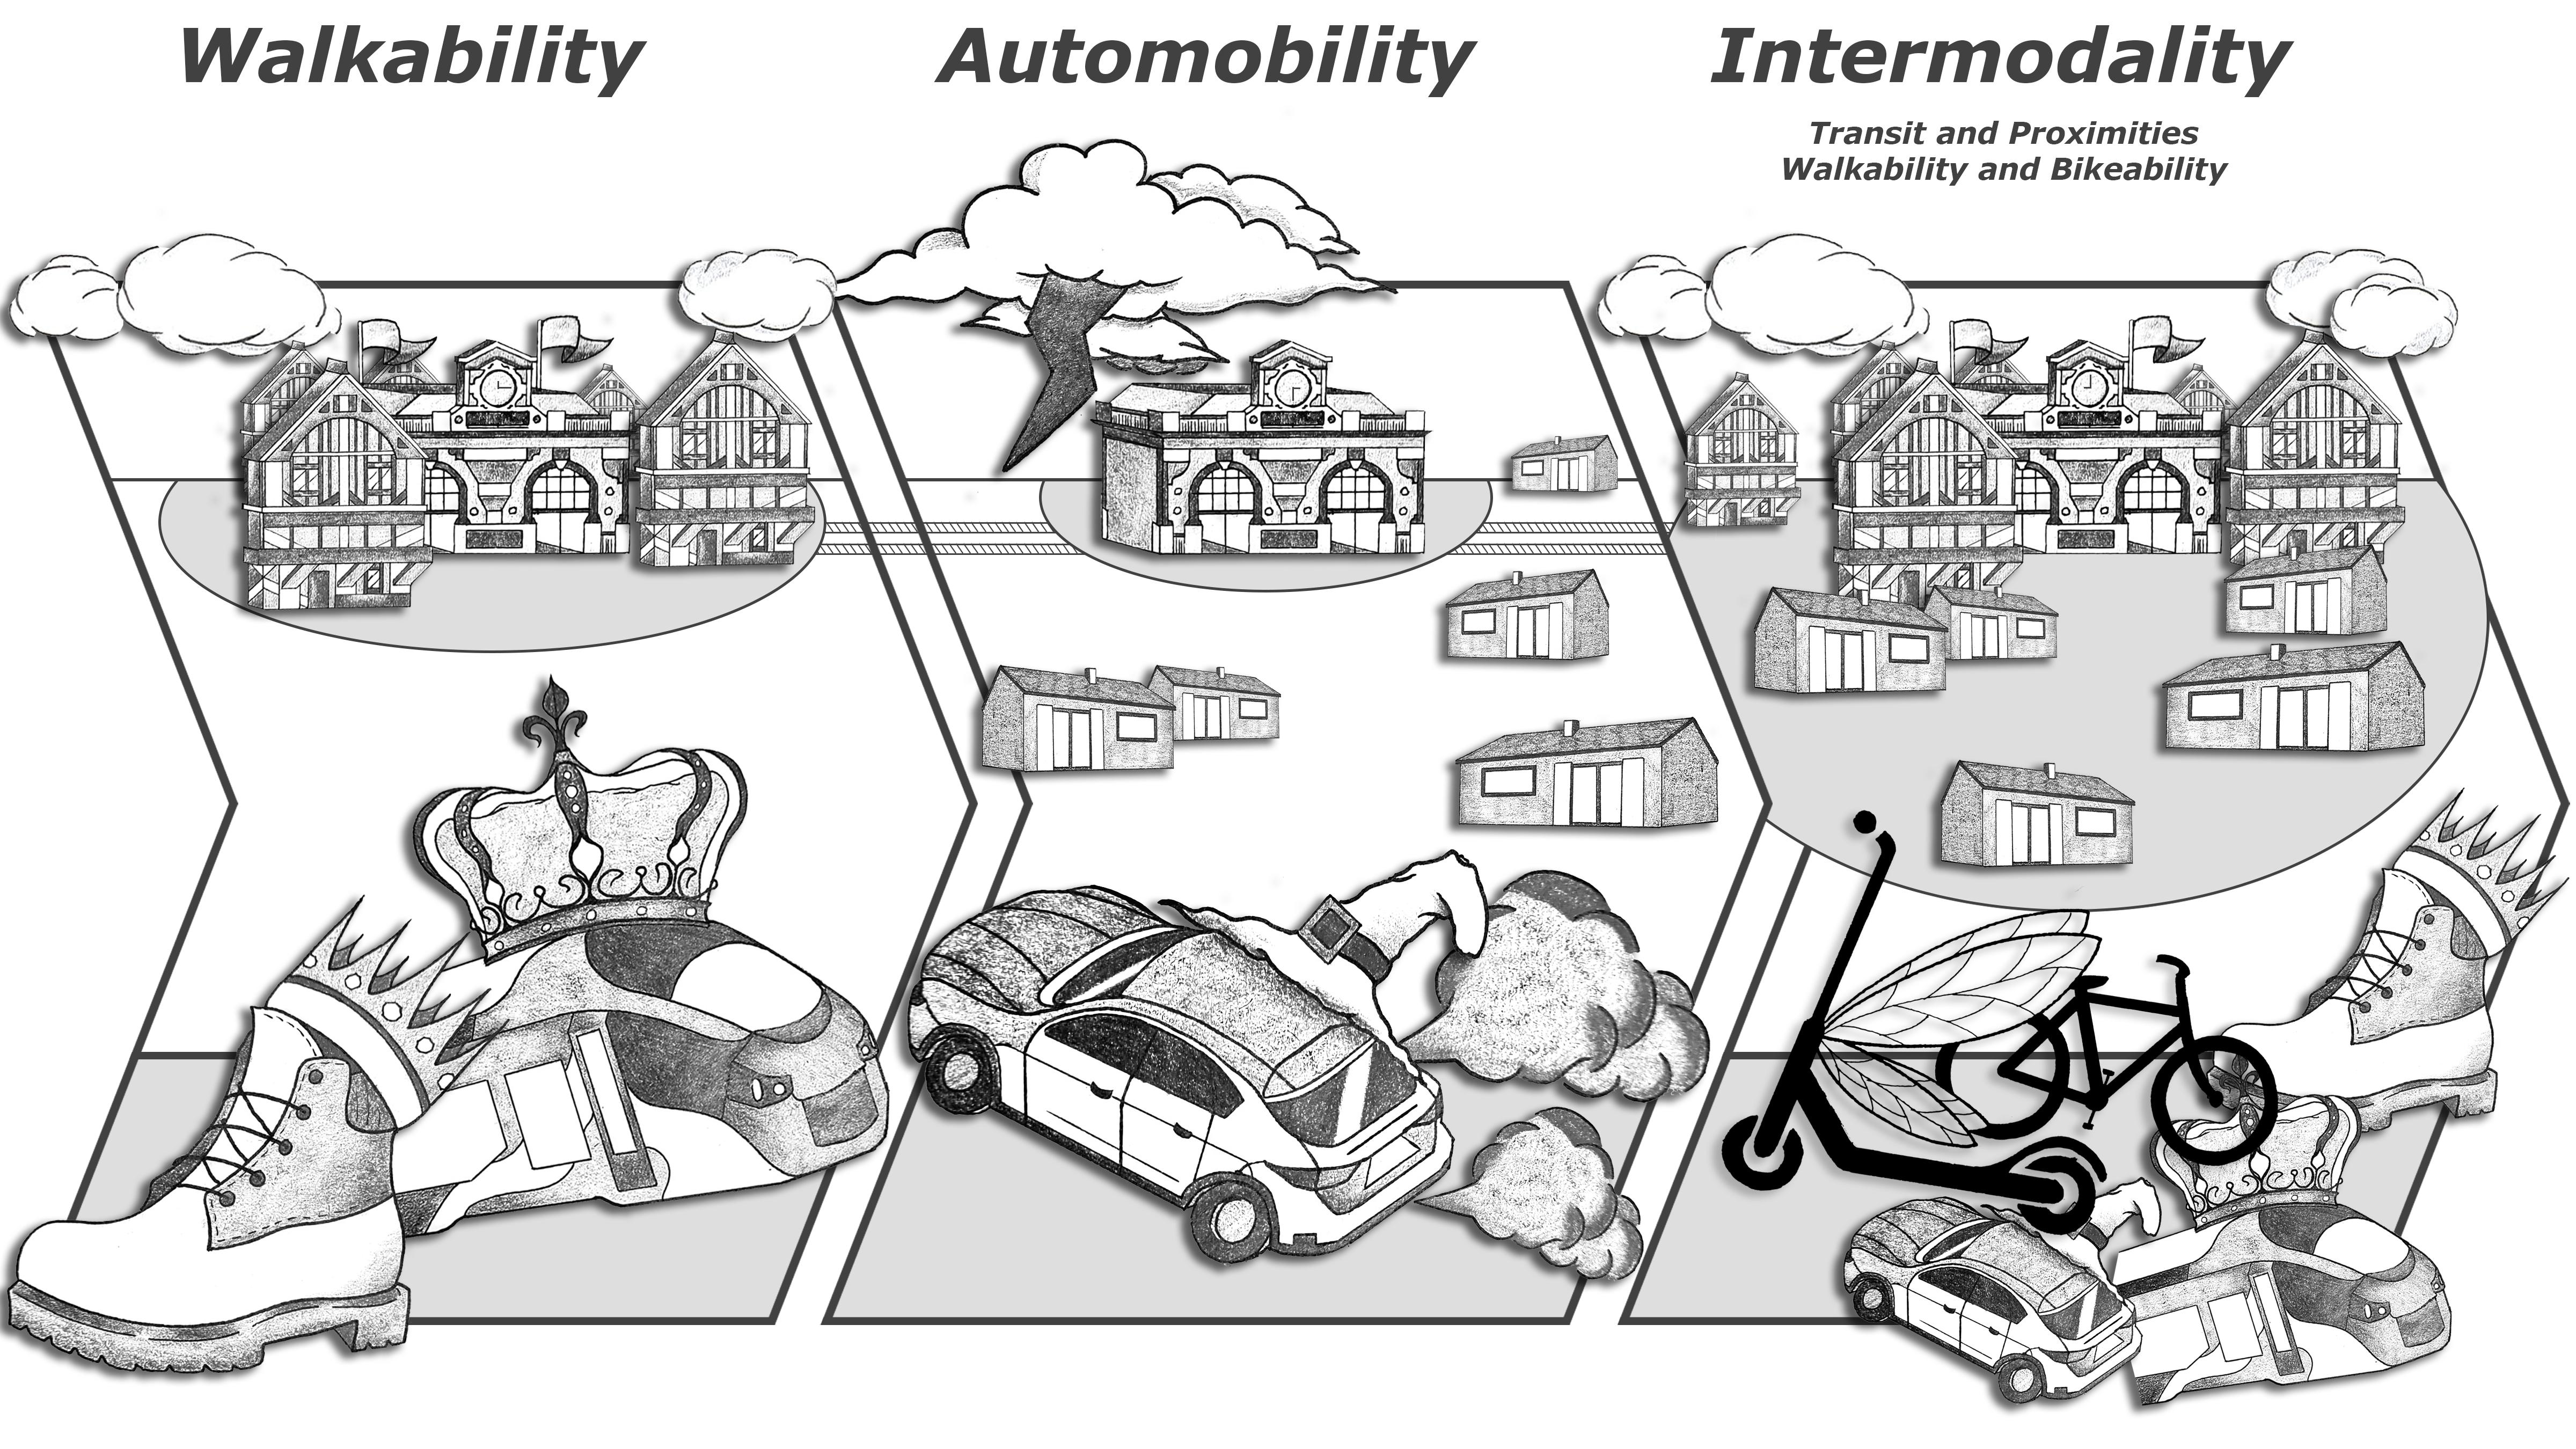
\includegraphics[width=1\columnwidth]{src/Figures/Preambule/EN_MT180_Illustration.jpg}}
        \vspace{5pt}
        \begin{flushright}\scriptsize{
        Author: \textcolor{blue}{Dylan Moinse (2022)}
        }\end{flushright}
    \end{figure}

%% ______________________________ %%
% INTRODUCTION
%------------------------------%
%% ✎ Dylan (V1) %%%%%%%%% ✅ %%
%% ✎ Alain (V2) %%%%%%%%% ✅ %%
%% ✎ Dylan (V3) %%%%%%%%% ✅ %%
%------------------------------%

\afterpage{%
%\afterpage{%

    % Arrière-plan introduction generale
    \AddToShipoutPictureBG*{%
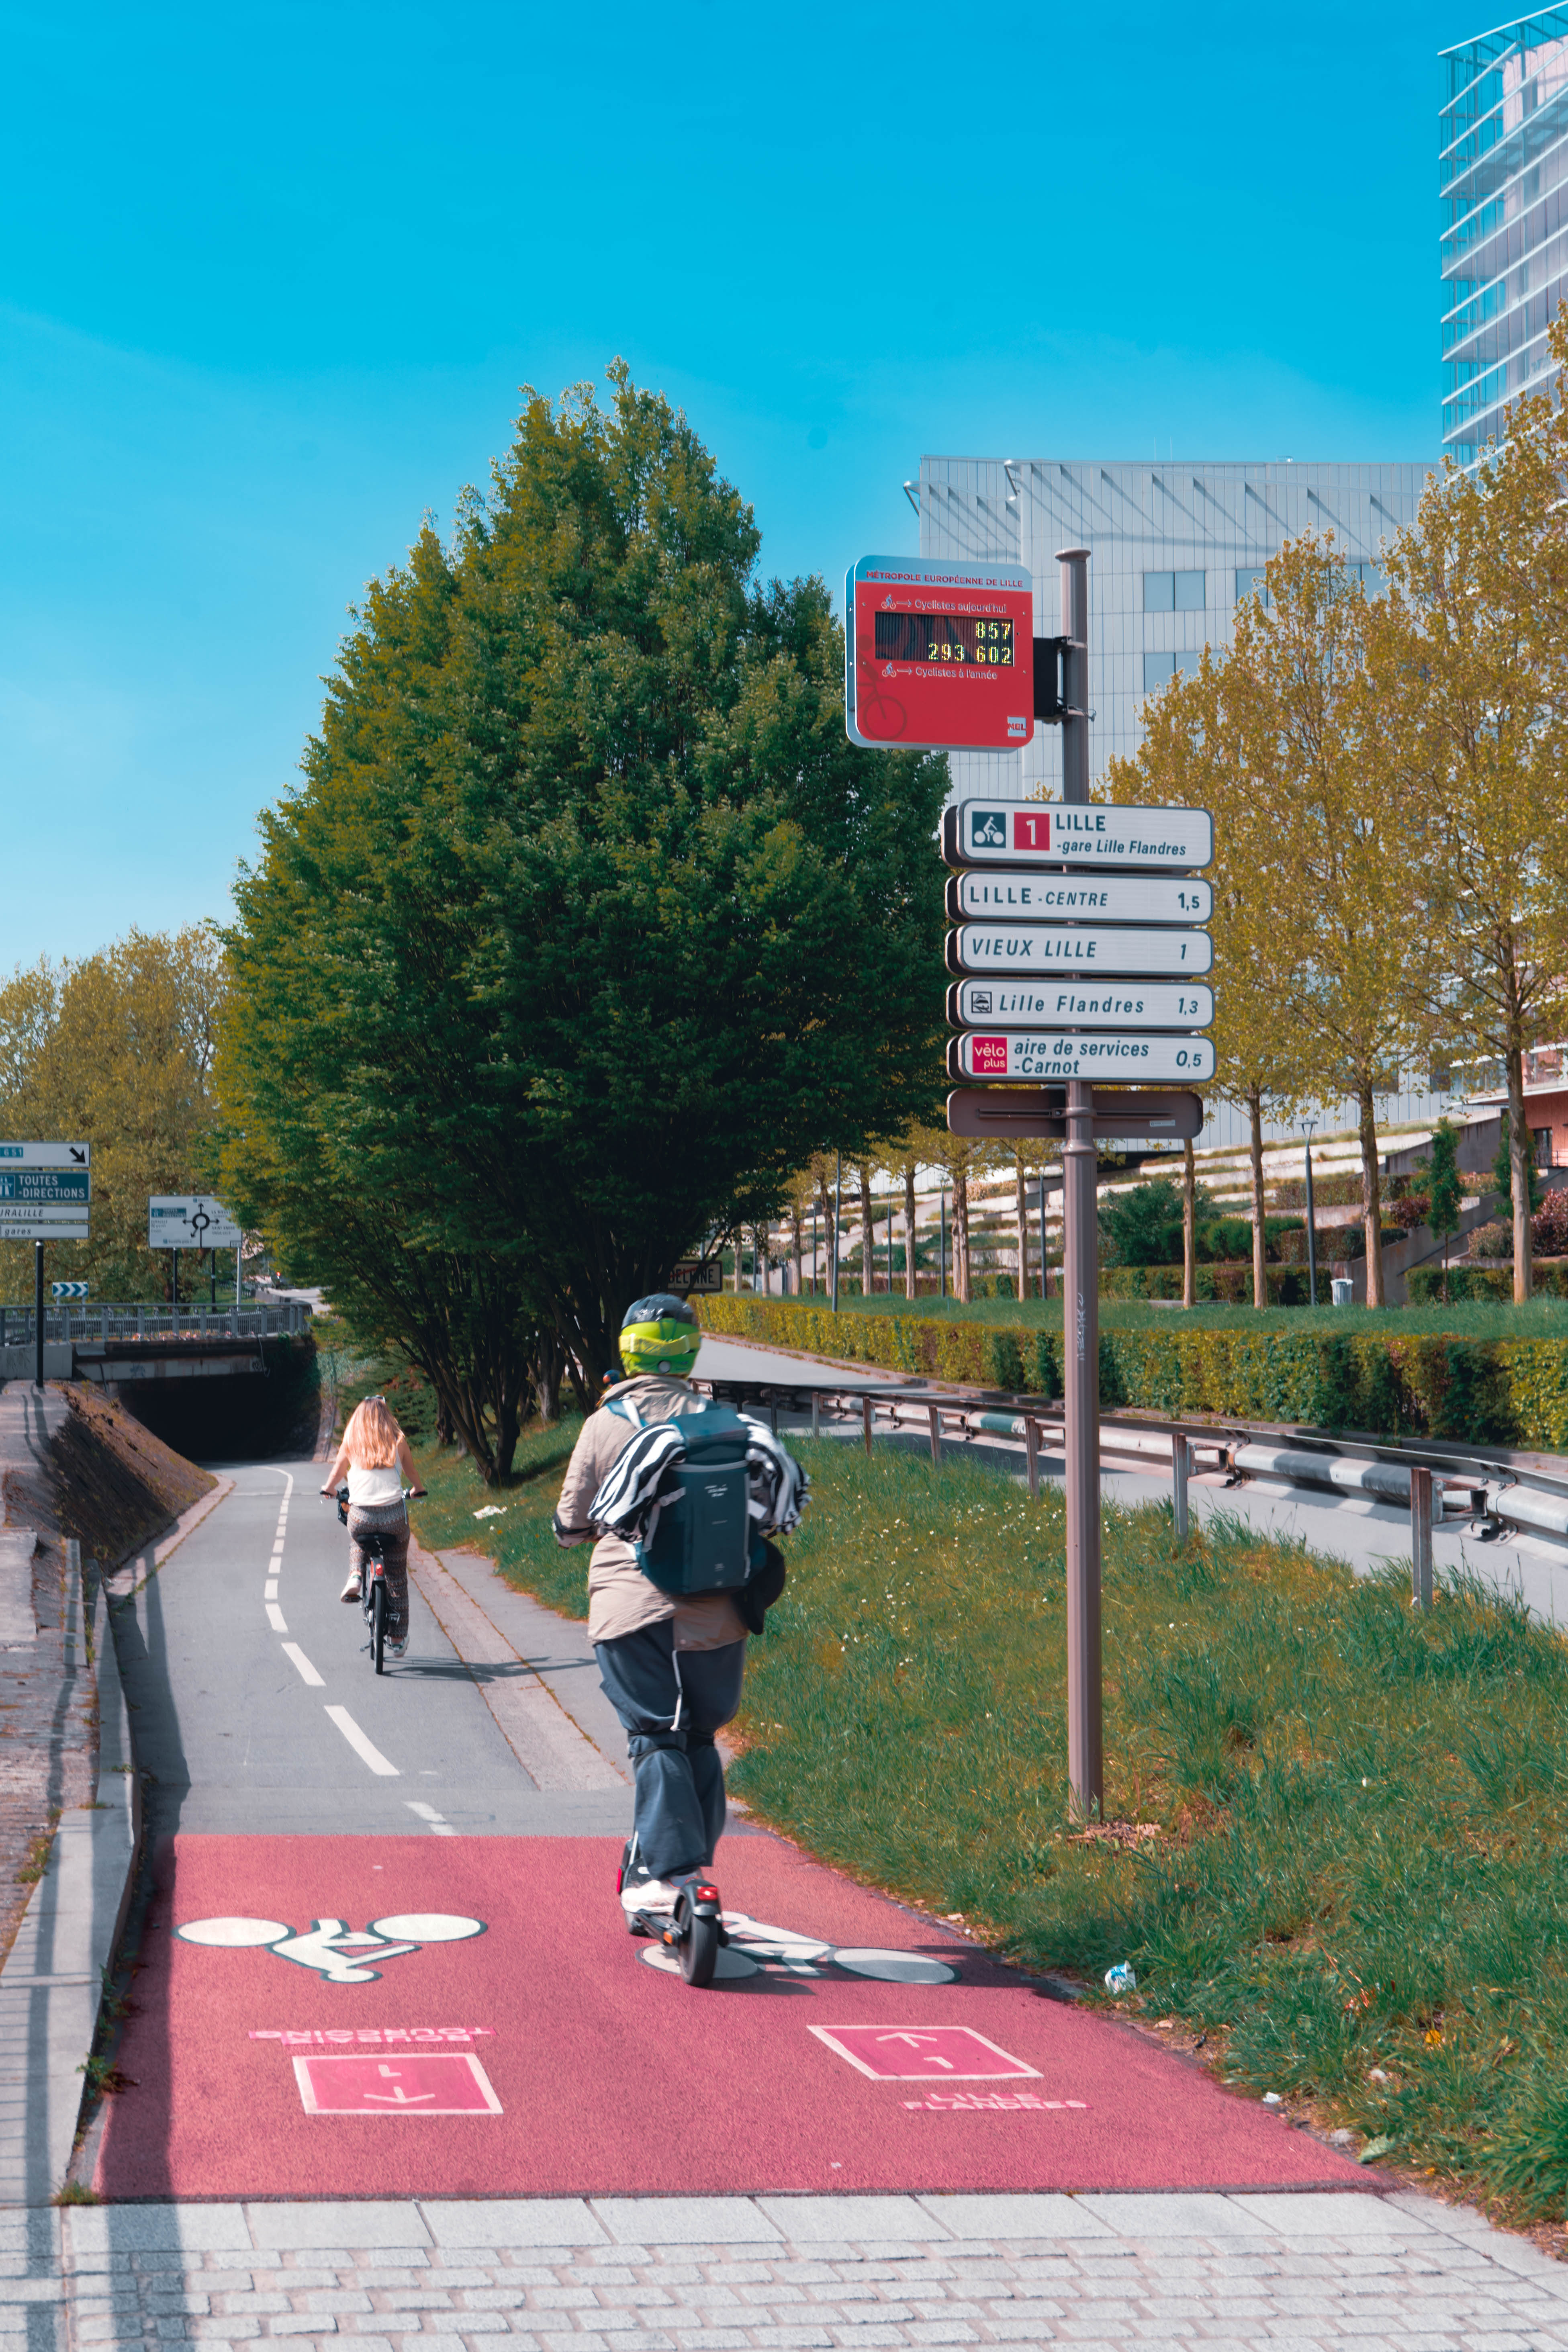
\includegraphics[width=\paperwidth,height=\paperheight]{src/Figures/Arriere_plan/Arriere_plan_Introduction.jpg}
    }

% Rectangle
\AddToShipoutPictureBG*{
  \begin{tikzpicture}[remember picture,overlay]
    \node[fill=white, opacity=0.75, text width=\paperwidth, minimum height=5cm, anchor=north] 
    at ([yshift=-9cm]current page.north) {};
  \end{tikzpicture}
}

% Source
\AddToShipoutPictureFG*{
  \AtPageLowerRight{
    \raisebox{1cm}{
      \hspace{16cm}
      
\begin{tikzpicture}
        \node[fill=white, rounded corners=5pt, inner sep=5pt, align=center] {
          \tiny{Photography: \textcolor{blue}{Dylan Moinse (2024)}}
        };
      \end{tikzpicture}
    }
  }
}
}%}

\renewcommand{\thefigure}{I.\arabic{figure}} % Numérotation spécifique pour l'introduction
\renewcommand{\thetable}{I.\arabic{table}}
\setcounter{figure}{0}

\pagenumbering{arabic}
\setcounter{page}{1} % Réinitialiser la numérotation à 1

    \needspace{1\baselineskip} % Réserve de l'espace
\part*{Introduction
    \label{body:introduction-generale}
    }
    %\addcontentsline{toc}{part}{Introduction}
    \markboth{Introduction}{}
    \markright{Introduction}{}
    \begin{refsegment}

    % Citation
    \begin{displayquote}
\Commas{\textsl{Keeping in mind that~–~for the same time and effort~–~someone can cycle five times farther than they can walk, these larger catchment areas actually play a critical role in feeding more customers into the public transport system. And they may~–~at least to a certain extent~–~tamp the demand for housing in and around train stations.} [\dots] \textsl{These investments in bicycle parking, rentals, and service make perfect economic sense for public transport agencies, as they increase ridership and revenue. Rather than treating the bicycle as a competitor, it is seen as an ally~–~one that connects passengers to their origin and destination; a critical component of the seamless door-to-door journey. These kinds of collective investments in a frequent and flexible public transport system~–~to maximize its convenience and coverage~–~are precisely what governments must do to lighten the financial burden of car ownership and break down the all-too-real barriers experienced by those lowest on the socioeconomic ladder.} [\dots] \textsl{in this case, we were no longer limited by the walking distance to shops, services, and public transport; nor were we forced to compete with the high demand for such proximity. With the extended range provided by pedal power, we could suddenly open up our search to entirely new parts of the city} [\dots] \textsl{An equitable region is one that provides residents with the same access to opportunity, regardless of their postal code. With a national rail network and national cycling network at our disposal, we know we can live virtually anywhere in the Randstad, without compromising on our lifestyle and our employment opportunities. And for us, that's a great place to be.}}

\textcolor{blue}{\textcite{bruntlett_curbing_2020}}\index{Bruntlett, Melissa|pagebf}\index{Bruntlett, Chris|pagebf}. \foreignlanguage{english}{\textsl{Curbing Traffic: The Human Case for Fewer Cars in Our Lives}, Island Press, p. 164-168.}%%Rédigé%%
    \end{displayquote}

% Hook
\lettrine[lines=3, findent=8pt, nindent=0pt]{\lettrinefont G}{\textbf{etting}} \textbf{the city back on rails} (\textsl{remettre la ville sur des rails}), such is the message conveyed by filmed anthropology, produced by \textcolor{blue}{Christian} \textcolor{blue}{\textcite{lallier_ville_2010}}\index{Lallier, Christian|pagebf}, French anthropologist and filmmaker. Titled \textsl{The City on Rails. The Utopia of the Metropolis} (\textsl{La ville sur des rails. L'utopie de la métropole}), this documentary explores the challenges of rail-oriented urbanism, brought back into focus \textcolor{blue}{\autocite[8]{lhostis_concevoir_2009}}\index{L'Hostis, Alain|pagebf}\index{Alexandre, Elsa|pagebf}\index{Appert, Manuel|pagebf}\index{Araud-Ruyant, Catherine|pagebf}\index{Basty, Marius|pagebf}\index{Biau, Géraldine|pagebf}\index{Bozzani-Franc, Sandra|pagebf}\index{Boutantin, Gratienne|pagebf}\index{Constantin, Chantal|pagebf}\index{Coralli, Monica|pagebf}\index{Durousset, Marie-Jeanne|pagebf}\index{Fradier, Christophe|pagebf}\index{Gabion, Cyrille|pagebf}\index{Leysens, Thomas|pagebf}\index{Mermoud, Françoise|pagebf}\index{Olny, Xavier|pagebf}\index{Perrin, Emmanuel|pagebf}\index{Robert, Jean|pagebf}\index{Simand, Noémie|pagebf}\index{Stransky, Vaclav|pagebf}\index{Soulas, Claude|pagebf}\index{Verdier, Anne-Marie|pagebf}\index{Vulturescu, Bogdan|pagebf} with the aim of reducing car dependency \textcolor{blue}{\autocites[15]{newman_ten_2000}[74]{motte-baumvol_territoires_2014}[4]{gallez_dependance_2018}}\index{Motte-Baumvol, Benjamin|pagebf}\index{Belton-Chevallier, Leslie|pagebf}\index{Morel-Brochet, Annabelle|pagebf}\index{Gallez, Caroline|pagebf}\index{Newman, Peter W.~G.|pagebf}\index{Kenworthy, Jeffrey~R.|pagebf}. Reflections and projects related to the dialectic between network and territory, that is, the interaction between territorial logics and network logics, have recently gained momentum \textcolor{blue}{\autocite[17]{gachon_impact_2019}}\index{Gachon, Mickaël|pagebf}, in a context where their coordination is becoming an essential part of urban \Commas{Sustainable Development} discourses \textcolor{blue}{\autocite[69]{nessi_politiques_2009}}\index{Nessi, Hélène|pagebf}\index{Delpirou, Aurélien|pagebf}, mainly leading to densification around train stations. These authors, however, raise questions about the systemic ability of rail to \Commas{correct the anomalies} inherited from territorial fragmentation \textcolor{blue}{\autocite[190]{ducharme_ville_2021}}\index{Ducharme, Olivier|pagebf} and the cultural dominance of \Commas{automobility} \textcolor{blue}{\autocites[57-58]{urry_sociology_2000}[28]{urry_system_2004}}\index{Urry, John|pagebf}.%%Translated%%

% Citation
Starting from these critiques regarding the adaptability limits of the \acrshort{TOD}, or transit-oriented development, particularly in areas shaped by the car-centered system, the central hypothesis is to explore the strategic role of bicycles and \gls{micromobility}, which show a lasting trend towards a \textquote{revival} \textcolor{blue}{\autocites[137-168]{heran_retour_2015}[3-28]{dusong_dynamiques_2021}[44]{eskenazi_voir_2022}}\index{Héran, Frédéric|pagebf}\index{Dusong, Clément|pagebf}\index{Papon, Francis|pagebf}\index{Eskenazi, Manon|pagebf}\index{Massot, \index{Eskenazi, Manon|pagebf}|pagebf} or are being reinvented \textcolor{blue}{\autocite[18]{amar_homo_2016}}\index{Amar, Georges|pagebf}. The aim of this doctoral research is to assess to what extent these modes of transport can fill the gaps of the originally formulated urban planning concept, by reconfiguring the interactions between proximity, public transport, and urban forms, from an intermodal perspective. In this regard, we consider the observed rise of cycling as an opportunity to effectively address the issue of \textquote{first and last miles} of public transportation. This thesis explores, in this sense, the windfall effect of the emergence of new mobility solutions within this family of individual and light vehicles \textcolor{blue}{\autocite[77]{oostendorp_combining_2018}}\index{Oostendorp, Rebekka|pagebf}\index{Gebhardt, Laura|pagebf}, to promote \textquote{smooth and door-to-door} journeys, as accurately summarized by the quote from \textcolor{blue}{\textcite[164-168]{bruntlett_curbing_2020}}\index{Bruntlett, Melissa|pagebf}\index{Bruntlett, Chris|pagebf}.%%Translated%%

% --- %
    % *.1. Context
    \needspace{1\baselineskip} % Reserve space
\section*{Cross-Perspectives on Territorial Organization and Spatial Mobility
    \label{introduction-generale:regards-croises-organisation-territoriale-mobilite-spatiale}
    }
    \addcontentsline{toc}{section}{Cross-Perspectives on Territorial Organization and Spatial Mobility}
    %\markboth{Cross-Perspectives on Territorial Organization and Spatial Mobility}{}
    \markright{Cross-Perspectives on Territorial Organization and Spatial Mobility}{}

% Context
The transport sector remains the leading source of \acrfull{GHG} emissions in France, accounting for 32\% of total national emissions in 2022 \textcolor{blue}{\autocite[41-53]{ministere_de_la_transition_ecologique_et_de_la_cohesion_des_territoires_chiffres_2024}}\index{Ministère de la Transition Écologique et de la Cohésion des Territoires@\textsl{Ministère de la Transition Écologique et de la Cohésion des Territoires}|pagebf}. Despite a general trend towards reducing carbon footprints across the country, the transport sector saw a 2.3\% increase in its carbon emissions over the year. This rise is mainly attributable to the use of private cars, which are responsible for more than half of these emissions, despite the frequent promises of technical and technological solutions. The unrestrained use of \textquote{auto-centrism} fits into a vicious cycle of automobile dependency, where European urban growth since the post-war period has been persistently shaped by its adaptation to the widespread use of cars. This process has led to the fragmentation of spaces, longer travel distances, and the structuring of networks, urban forms, and land uses, creating territorial vulnerabilities. As a result, the paradigm of \textquote{sustainable mobility} or \textquote{mobility transition} and, more broadly, its \textquote{decarbonization}, is primarily a matter of urban planning \textcolor{blue}{\autocite{societe_francaise_des_urbanistes_decarbonation_2024}}\index{Société française des urbanistes@\textsl{Société française des urbanistes}|pagebf}. In this sense, the train station district serves as a strategic junction between the city and transport, drawing the focus of urban planners. To \textquote{reweave} the city, public transport must be seen as the structural element of corridors and neighborhoods, a pivot from which urban development actors are invited to rethink the organization of territories \textcolor{blue}{\autocite[8]{boisclair_retisser_2013}}\index{Boisclair, Catherine|pagebf}.%%Translated%%

% TOD
Rising to the level of an action reference, the issue of coordination between urban planning and transport, beyond the \textquote{myth of coherence}, introduces the theoretical and operational model of \acrfull{TOD} \textcolor{blue}{\autocite[183-220]{gallez_mythes_2010}}\index{Gallez, Caroline|pagebf}\index{Kaufmann, Vincent|pagebf}\index{Guerrinha, Christophe|pagebf}\index{Maksim, Hanja-Niriana|pagebf}\index{Thébert, Mariane|pagebf}, in which the technical object and its environment interact in co-construction over time \textcolor{blue}{\autocite[44-50]{leheis-guillot_ville_2011}}\index{Leheis-Guillot, Stéphanie|pagebf}. This integrated approach, which involves simultaneously thinking about the city and transport, relies on a mechanism of bidirectional and continuous interaction, embedded in a feedback loop \textcolor{blue}{\autocite[130]{wegener_overview_2004}}\index{Wegener, Michael|pagebf}. It is within this systemic framework that we support the hypothesis that \acrshort{TOD} would benefit from better integrating the proximities generated by train station districts, both in terms of flow polarization and urban insertion opportunities. Just like the title chosen by the British researcher \textcolor{blue}{Rich~C.} \textcolor{blue}{\textcite[40]{mcilroy_this_2023}}\index{McIlroy, Rich~C.|pagebf}, in his article \textsl{This is where public transport falls down}\footnote{
    \textsl{This is where public transport falls down} \textcolor{blue}{\autocite[40]{mcilroy_this_2023}}\index{McIlroy, Rich~C.|pagebf}.
}, the primary challenge of \acrshort{TOD} today is less about improving the quality of public transport and intensifying human activities around exchange hubs, than it is about enhancing the pathways to and from these nodes. In short, while hopes for decarbonizing mobility focus on the \textquote{magic triptych} – composed of the car, whether electric, shared, autonomous, or connected – it seems likely that this focus on the automobile, whose rebound effects and persistent nuisances are underestimated, will prove insufficient. Conversely, the focus should be on the synergy between walking, \gls{bicycle}, and public transport, a more fitting \textquote{intermodal triptych} capable of addressing contemporary urban mobility challenges and territorial planning \textcolor{blue}{\autocite[1]{soulas_triptyque_2021}}\index{Soulas, Claude|pagebf}.%%Translated%%

% Light Individual Mobility + Research Topic
The urban model of \acrshort{TOD} aims to link two distinct scales of daily mobility: on one hand, metropolitan and regional mobility, structured by public transport networks, and on the other hand, proximity mobility, which prioritizes walking and cycling as much as possible \textcolor{blue}{\autocites[81]{conesa_modelisation_2010}[124]{lo_feudo_scenario_2014}}\index{Lo Feudo, Fausto|pagebf}\index{Menerault, Philippe|pagebf}\index{L'Hostis, Alain|pagebf}\index{Festa, Demetrio Carmine|pagebf}\index{Conesa, Alexis|pagebf}\index{Paris, Didier|pagebf}. However, over the last decade, bicycles and micromobility have diversified to the point that they tend to \textquote{hybridize}, evolving into individual, transportable objects \textcolor{blue}{\autocite[20]{amar_du_2012}}\index{Amar, Georges|pagebf}, such as \acrfull{PeS}, or resembling individual public transport systems \textcolor{blue}{\autocites[179]{amar_homo_2010}[4]{castex_prise_2017}}\index{Castex, Élodie|pagebf}\index{Frère, Séverine|pagebf}\index{Groux, Annette|pagebf}\index{Amar, Georges|pagebf}, similar to shared mobility. Through innovation processes driving socio-spatial transformations \textcolor{blue}{\autocite[89]{ageron_intermodalite-voyageurs_2013}}\index{Ageron, Pierre|pagebf}\index{Varlet, Jean|pagebf}, what we call \textquote{light individual mobility} is integrated into the public transport network as a complementary modal offer. Its intermodal uses are intrinsically linked to temporal and spatial dimensions, leading us to develop a reflection informed by references to spaces, territories, and places \textcolor{blue}{\autocite[4]{sebban_complementarite_2003}}\index{Sebban, Annie-Claude|pagebf}\index{Motte, Alain|pagebf}. It is from these considerations that we have established our research topic, entitled:
    \begin{displayquote}
\textbf{The Transit-Oriented Development Urban Model Revisited by Emerging Light Individual Mobility. An Investigation in the Hauts-de-France Region.}
    \end{displayquote}%%Translated%%

% --- %
    % *.2. Scientific Positioning
    \needspace{1\baselineskip} % Reserve space
\section*{Scientific Positioning
    \label{introduction-generale:positionnement-scientifique}
    }
    \addcontentsline{toc}{section}{Scientific Positioning}
    %\markboth{Scientific Positioning}{}
    \markright{Scientific Positioning}{}

% Train Station
This thesis adopts a planning approach, mobilizing elements from the \textquote{urban fabric} with a specific focus on the materiality of public spaces. As a general hypothesis, we adopt the concept of \textquote{networked urbanism} or \textquote{city of networks} as the analytical framework, considered as explanatory models of urban transformations \textcolor{blue}{\autocite[]{dupuy_urbanisme_1991}}\index{Dupuy, Gabriel|pagebf}. This framework is based on the assumption that territorial organization, made possible by networks, offers a multiplicity of connections, the optimization of which is a condition for its effectiveness. In this regard, the train station is considered as a \textquote{territorial object} \textcolor{blue}{\autocite[7]{moretti_interconnexion_1999}}\index{Moretti, Anna|pagebf}\index{Vacheret, Guy|pagebf}, a space at the interface of transport networks and urban dynamics. This concept aligns with a recent trend in urban studies aiming to reconsider the role of train stations in the structuring of contemporary cities, a \textquote{return of train stations in urban studies} \textcolor{blue}{\autocite[489]{delage_gare_2013}}\index{Delage, Aurélie|pagebf}. Far from being reduced to a mere functional connection point, the train station is viewed here in all its complexity as a \textquote{station-system} \textcolor{blue}{\autocites[395]{le_bot_quel_2019}{le_bot_management_2020}}\index{Le Bot, Nils|pagebf}. This stance integrates its spatial, organizational, and symbolic dimensions, recognizing its structuring role not only for transport networks but also for urban production and organization, as well as the lifestyles associated with it. Furthermore, the research topic is framed as transcending scales \textcolor{blue}{\autocite[3]{knowles_transit_2019}}\index{Knowles, Richard~D.|pagebf}\index{Ferbrache, Fiona|pagebf}, promoting the interlocking of temporal and scalar scales; from land and economic evolution to urban projects; from the local scale of the building-passenger to regional and (inter)national dimensions \textcolor{blue}{\autocites[13-14]{menerault_gares_2001}[238]{chapelon_transports_2016}}.%%Translated%%

% Proximities
This reflection on the train station cannot be dissociated from the mobilities it polarizes. As such, this research involves a shift in analysis, moving from the train station object to the geographical proximities it generates, incorporating a reflection on light individual mobility and its role in the structuring of train station districts. This shift in focus is part of a broader paradigmatic change in mobility analysis, to which the train station actively contributes \textcolor{blue}{\autocite[53]{leheis-guillot_ville_2011}}\index{Leheis-Guillot, Stéphanie|pagebf}. This \textquote{mobility turn} \textcolor{blue}{\autocites{sheller_new_2006}[8]{sheller_mobilizing_2016}[13]{randell_no_2020}}\index{Sheller, Mimi|pagebf}\index{Urry, John|pagebf}\index{Randell, Richard|pagebf} emphasizes the relational and systemic dimension of the \gls{journey}, beyond a strictly infrastructural approach \textcolor{blue}{\autocite[14]{heran_retour_2015}}\index{Héran, Frédéric|pagebf}. In this framework, this thesis sits at the intersection of several research fields, combining urban planning, territorial development, geography, sociology, and data science, in order to question the reconfiguration of \acrshort{TOD} under the effect of (new) proximities made possible by the integration of light individual mobility. This approach leads to considering this mobility as a strategic lever for the revitalization of \acrshort{TOD} in urban contexts inherited from the car-oriented model \textcolor{blue}{\autocite[209]{heran_retour_2015}}\index{Héran, Frédéric|pagebf}. It is thus part of a broader reflection on the renewal of public transport and urban planning policies, in the face of the challenges of the \textquote{first and last miles}. It highlights the opportunity that light individual mobility represents for promoting a multimodal and \textquote{door-to-door} mobility system \textcolor{blue}{\autocite[979]{lee_bicycle-based_2016}}\index{Lee, Jaeyeong|pagebf}\index{Choi, Keechoo|pagebf}\index{Leem, Yountaik|pagebf}.%%Translated%%

% Positioning
This doctoral research thus mobilizes four complementary approaches to structure our investigation: (i) the approach through technical objects, by analyzing the \textquote{station-system} and the associated modes of transport; (ii) the approach through uses and intermodal practices, by studying the modal behaviors and strategies of cycling passengers; (iii) the approach through \gls{accessibility}, by measuring the effects of light individual mobility on accessibility; and (iv) the approach through urban systems, by questioning the effects of light individual mobility on railway urban planning. Thus, the train station cannot be reduced to a purely socio-technical object \textcolor{blue}{\autocite[]{joseph_villes_1999}}\index{Joseph, Isaac|pagebf}, but must also be considered as an urban object, taking into account its territorial integration, beyond the scale of the building-passenger or its immediate environment. It plays a spatial, functional, and symbolic role, acting both as a \textquote{stage} and an \textquote{actor} \textcolor{blue}{\autocite[5]{baron_gares_2016}}\index{Baron, Nacima|pagebf}\index{Roseau, Nathalie|pagebf}. This approach thus allows for exploring the potential for revising \acrshort{TOD} through the integration of light individual mobility. It offers a renewed perspective on train station districts and their role in urban organization, while contributing to the formalization of an expanded model: an \acrfull{M-TOD}, or a transit-oriented development model that integrates light individual mobility.%%Translated%%

% --- %
    % *.3. Research Directions
    \needspace{1\baselineskip} % Reserve space
\section*{Research Directions
    \label{introduction-generale:problematique-objectifs-hypotheses}
    }
    \addcontentsline{toc}{section}{Research Directions}
    %\markboth{Research Problem, Objectives, and Hypotheses}{}
    \markright{Research Problem, Objectives, and Hypotheses}{}

% Research Problem
This thesis aims to examine the transformations of the \acrshort{TOD} model from the perspective of light individual mobility, adopting a theoretical, empirical, and forward-looking approach to determine and establish an optimal framework for \gls{intermodal accessibility}. Our central question is framed as follows:
    \begin{displayquote}
\textbf{To what extent can the integration of light individual mobility address the challenges of the \textquote{first and last miles} of public transport and contribute to enhancing the intermodal accessibility of train station districts in the Hauts-de-France region? \\
How do these \textquote{proximities} reconfigure the urban model of \textsl{Transit-Oriented Development} and pave the way for a \textsl{Micromobility-friendly Transit-Oriented Development}, better suited to urban realities and evolving mobility practices? \\
What are the conditions for implementation and the levers of action to be mobilized to ensure optimal integration of light individual mobility into urban planning and transport strategies?}
    \end{displayquote}%%Translated%%

% Objectives
This line of questioning will guide the structure of our research, showing how light individual mobility can enrich the \acrshort{TOD} model and the implications this has for mobility and territorial planning. Throughout our doctoral project, we will develop a progressive approach in several stages, designed to revisit the \acrshort{TOD} in light of the proximities renewed by the development of light individual mobility. Each chapter is based on a research objective, articulating both theoretical and empirical reflections on the challenges of intermodal accessibility (see the \hyperref[fig-introduction:objectifs-hypotheses]{diagram~\ref{fig-introduction:objectifs-hypotheses}}, page~\pageref{fig-introduction:objectifs-hypotheses}). To structure our reasoning, we use the \acrfull{QQOQCCP} questioning method, which allows us to clarify the contours and objectives of our research:
        \begin{customitemize}
    \item \textsl{What} and \textsl{When}? ({\textcolor{blue}{\(O_1\)}\label{objectif-1}}). The first chapter lays the conceptual and historical foundations of \acrshort{TOD} and cycling, identifying their strengths and limitations. It aims to introduce the essential nature of an \acrshort{M-TOD}, that is, a revised model that takes into account this intermodal component;
    \item \textsl{By whom} and \textsl{On what}? ({\textcolor{blue}{\(O_2\)}\label{objectif-2}}). The second chapter aims to build an analytical framework by reviewing existing scientific and technical works on light individual mobility, \gls{intermodality}, and the rethinking of \acrshort{TOD}. It puts international experiences and new knowledge on intermodality into perspective;
    \item \textsl{Where} and \textsl{With what}? ({\textcolor{blue}{\(O_3\)}\label{objectif-3}}). The third chapter uses mixed methods to construct and analyze empirical data within a defined geographical area. It aims to define, adapt, and relate appropriate approaches to propose a \textquote{custom survey};
    \item \textsl{Who} and \textsl{How many}? ({\textcolor{blue}{\(O_4\)}\label{objectif-4}}). The fourth chapter measures and characterizes intermodal practices, focusing on the profiles of users who combine the use of light individual mobility and public transport. It aims to quantify the flows and identify the socio-demographic and environmental factors influencing such modal choices;
    \item \textsl{Where to} and \textsl{Why}? ({\textcolor{blue}{\(O_5\)}\label{objectif-5}}). The fifth chapter aims to measure and explain the spatial extension of train station districts through light individual mobility. It evaluates the accessibility gains at different scales;
    \item \textsl{How} and \textsl{In relation to what}? ({\textcolor{blue}{\(O_6\)}\label{objectif-6}}). The final chapter proposes a conceptual and operational formalization of the \acrshort{M-TOD} by modeling the conditions for its implementation. It aims to formulate recommendations for urban development stakeholders.
        \end{customitemize}%%Translated%%

% Figure research objectives and hypotheses
    \begin{figure}[h!]\vspace*{4pt}
        \caption{Overview of Research Objectives and Hypotheses}
        \label{fig-introduction:objectifs-hypotheses}
        \centerline{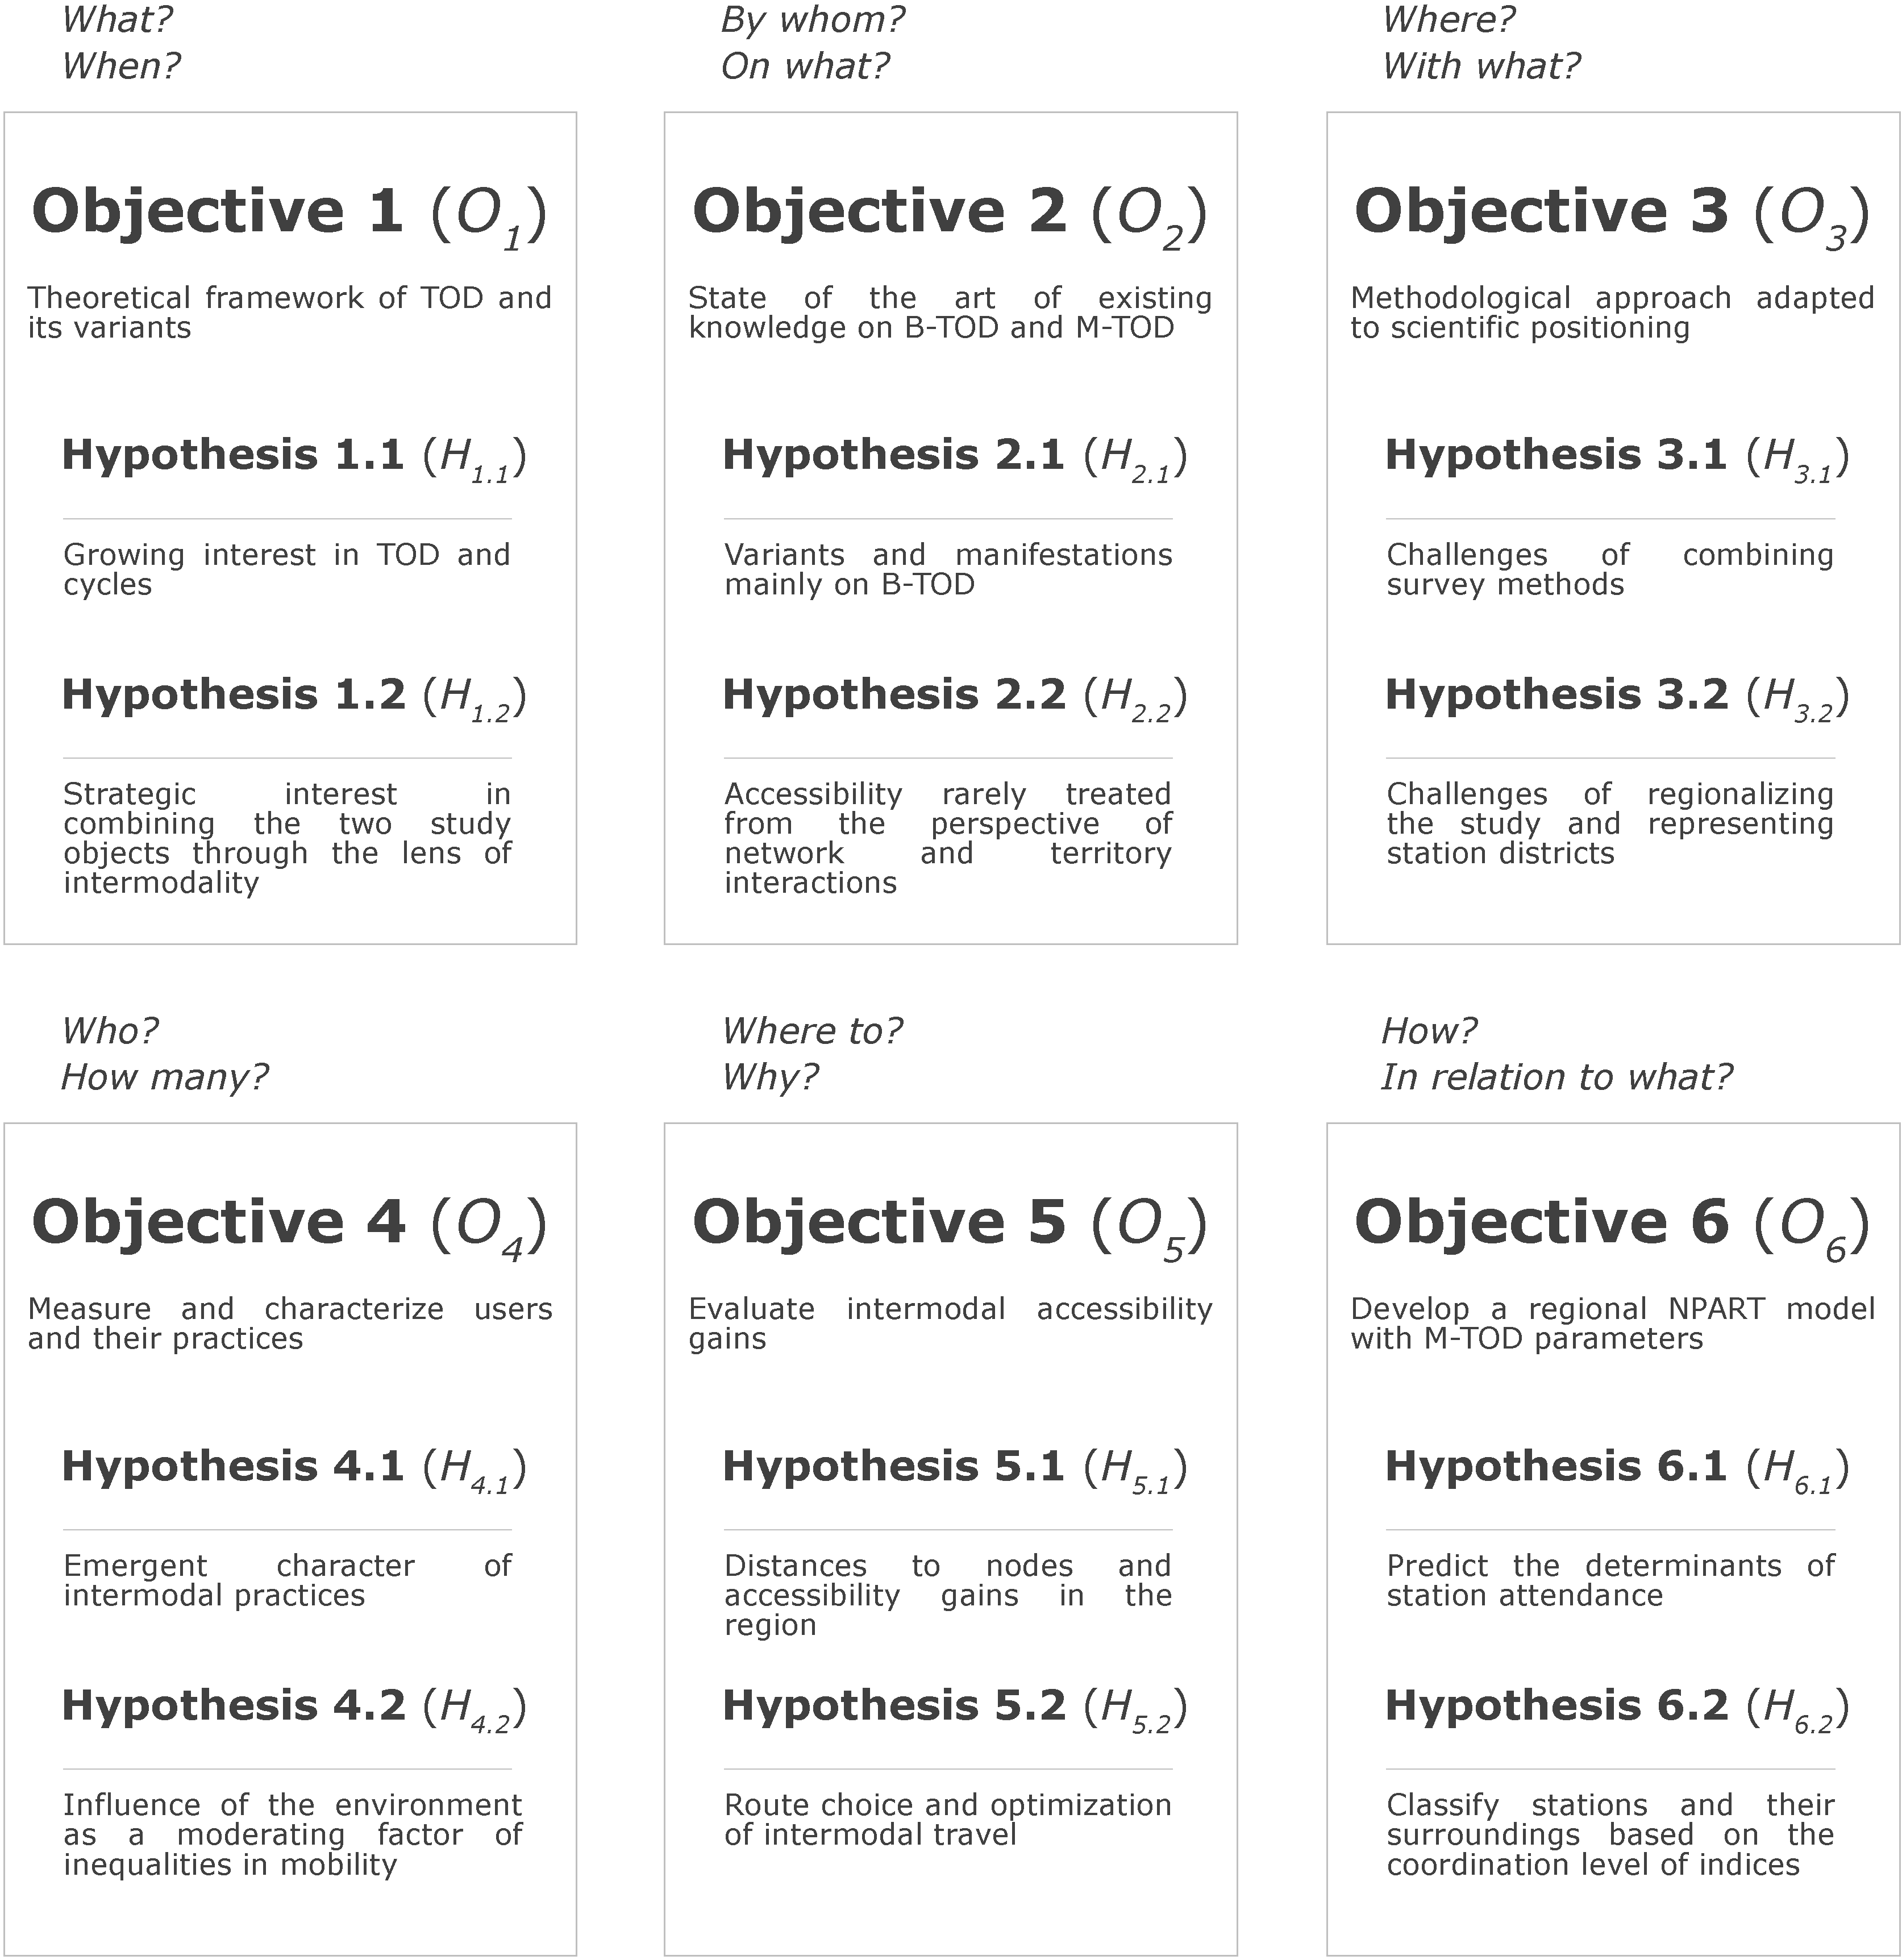
\includegraphics[width=1\columnwidth]{src/Figures/Introduction/EN_Objectifs_recherche.pdf}}
        \vspace{5pt}
        \begin{flushright}\scriptsize{
        Author~: \textcolor{blue}{Dylan Moinse (2023)}
        }\end{flushright}
    \end{figure}

% Hypotheses
Based on the previously defined objectives, which structure the various chapters of this thesis, the research hypotheses emerge, constituting the thread of our argument throughout this scientific work (see the \hyperref[fig-introduction:objectifs-hypotheses]{diagram~\ref{fig-introduction:objectifs-hypotheses}}, page~\pageref{fig-introduction:objectifs-hypotheses}). These hypotheses are based on a hypothetico-deductive approach and are characterized by their associative, complex, and directional nature\footnote{
    According to \textcolor{blue}{\textcite[41-43]{tomini_methodes_2020}}\index{Tomini, Luca|pagebf}\index{Wintgens, Sophie|pagebf}, in their handbook \textsl{Méthodes d'enquêtes de terrain en sciences sociales}, associative hypotheses postulate an interactive relationship between concepts; complex hypotheses, on the other hand, specify a relationship between multiple concepts; while directional hypotheses formulate the orientation of the links that connect these concepts.
} \textcolor{blue}{\autocite[43]{tomini_methodes_2020}}\index{Tomini, Luca|pagebf}\index{Wintgens, Sophie|pagebf}. Based on these objectives, we propose the following hypotheses to guide our reflection:
        \begin{customitemize}
    \item \textsl{Emerging research themes related to \textsl{Transit-Oriented Development} and light individual mobility deserve to be considered jointly} ({\textcolor{blue}{\(H_1\)}\label{hypothese-1}}). Indeed, both of these axes are attracting growing interest in both academic and operational spheres ({\textcolor{blue}{\(S.H_{1.1}\)}\label{sous-hypothese-1.1}}) and would benefit from being studied in an articulated manner to reveal their potential synergies ({\textcolor{blue}{\(S.H_{1.2}\)}\label{sous-hypothese-1.2}})~;
    \item \textsl{Current knowledge on this intermodal synergy remains strongly conditioned by the bicycle and train combination, and is rarely analyzed through the lens of \textsl{Transit-Oriented Development}} ({\textcolor{blue}{\(H_2\)}\label{hypothese-2}}). Existing work primarily focuses on the bicycle object ({\textcolor{blue}{\(S.H_{2.1}\)}\label{sous-hypothese-2.1}}), while accessibility issues are mostly addressed from a strictly transport-related perspective ({\textcolor{blue}{\(S.H_{2.2}\)}\label{sous-hypothese-2.2}})~;
    \item \textsl{Understanding the complexity of intermodal dynamics and their implications on the urban environment faces the challenge of defining an analytical methodology} ({\textcolor{blue}{\(H_3\)}\label{hypothese-3}}). Given the gaps identified in the literature, it seems relevant to employ a mixed-methods approach, combining various survey techniques ({\textcolor{blue}{\(S.H_{3.1}\)}\label{sous-hypothese-3.1}}). Moreover, adopting a regional study area and redefining the concept of train station districts in line with the principles of \acrshort{TOD} are necessary adjustments ({\textcolor{blue}{\(S.H_{3.2}\)}\label{sous-hypothese-3.2}})~;
    \item \textsl{Intermodal practices are experiencing significant growth due to the combined emergence of new mobility solutions, although these practices are marked by differentiated appropriation across various social groups} ({\textcolor{blue}{\(H_4\)}\label{hypothese-4}}). The development of intermodality involving cycling and public transport is part of a diversification and appropriation process of mobility modes ({\textcolor{blue}{\(S.H_{4.1}\)}\label{sous-hypothese-4.1}}). However, this appropriation remains uneven, with certain social groups adopting these modes more easily than others, a situation that could be mitigated through territorial planning interventions ({\textcolor{blue}{\(S.H_{4.2}\)}\label{sous-hypothese-4.2}})~;
    \item \textsl{Integrating light individual mobility within public transport networks is a major lever for improving regional accessibility} ({\textcolor{blue}{\(H_5\)}\label{hypothese-5}}). This integration increases the reach of trips, extending the service areas of train station districts and facilitating access to destinations ({\textcolor{blue}{\(S.H_{5.1}\)}\label{sous-hypothese-5.1}}). Additionally, it promotes the optimization of routes, making intermodal travel more competitive compared to car use, including for long-distance daily mobility ({\textcolor{blue}{\(S.H_{5.2}\)}\label{sous-hypothese-5.2}})~;
    \item \textsl{Expanding the concept of urban planning to include light individual mobility is a lever for revitalizing train station districts, enhancing their accessibility in a broader sense} ({\textcolor{blue}{\(H_6\)}\label{hypothese-6}}). Certain factors related to the cyclability of train station districts help stimulate demand around exchange hubs ({\textcolor{blue}{\(S.H_{6.1}\)}\label{sous-hypothese-6.1}}), while making them more consistent with the guiding principles of \acrshort{TOD} ({\textcolor{blue}{\(S.H_{6.2}\)}\label{sous-hypothese-6.2}}).
\end{customitemize}%%Translated%%

% --- %
    % *.4. Methodology
    \needspace{1\baselineskip} % Reserve space
\section*{Research Strategy
    \label{introduction-generale:methodologie}
    }
    \addcontentsline{toc}{section}{Research Strategy}
    %\markboth{Methodology}{}
    \markright{Methodological Framework}{}

% Introduction
In order to address the research problem and the formulated objectives and hypotheses, this thesis adopts a mixed methodological approach, combining original methods tailored to the specifics of the subject under study (see the \hyperref[fig-introduction:methodes-hypotheses]{diagram~\ref{fig-introduction:methodes-hypotheses}}, page~\pageref{fig-introduction:methodes-hypotheses}). This methodological approach enables the articulation of three essential dimensions: (i) a conceptual reflection on the evolution of \acrshort{TOD} and its relationship with light individual mobility; (ii) an investigation into existing intermodal practices and the factors influencing these mobility behaviors; and (iii) an assessment of the effects of light individual mobility on accessibility to train stations and on the structuring of surrounding districts, within a regional scope. Far from being a linear approach, this methodological path embraces its complexity, mobilizing complementary tools in order to capture the multiple dimensions of \acrshort{TOD} and light individual mobility, in accordance with the \hyperref[hypothese-3]{hypothesis~\(H_3\)} (page~\pageref{hypothese-3}).%%Translated%%

% Figure methodology hypotheses
    \begin{figure}[h!]\vspace*{4pt}
        \caption{Methodological Framework Designed in Dialogue with the Research Hypotheses}
        \label{fig-introduction:methodes-hypotheses}
        \centerline{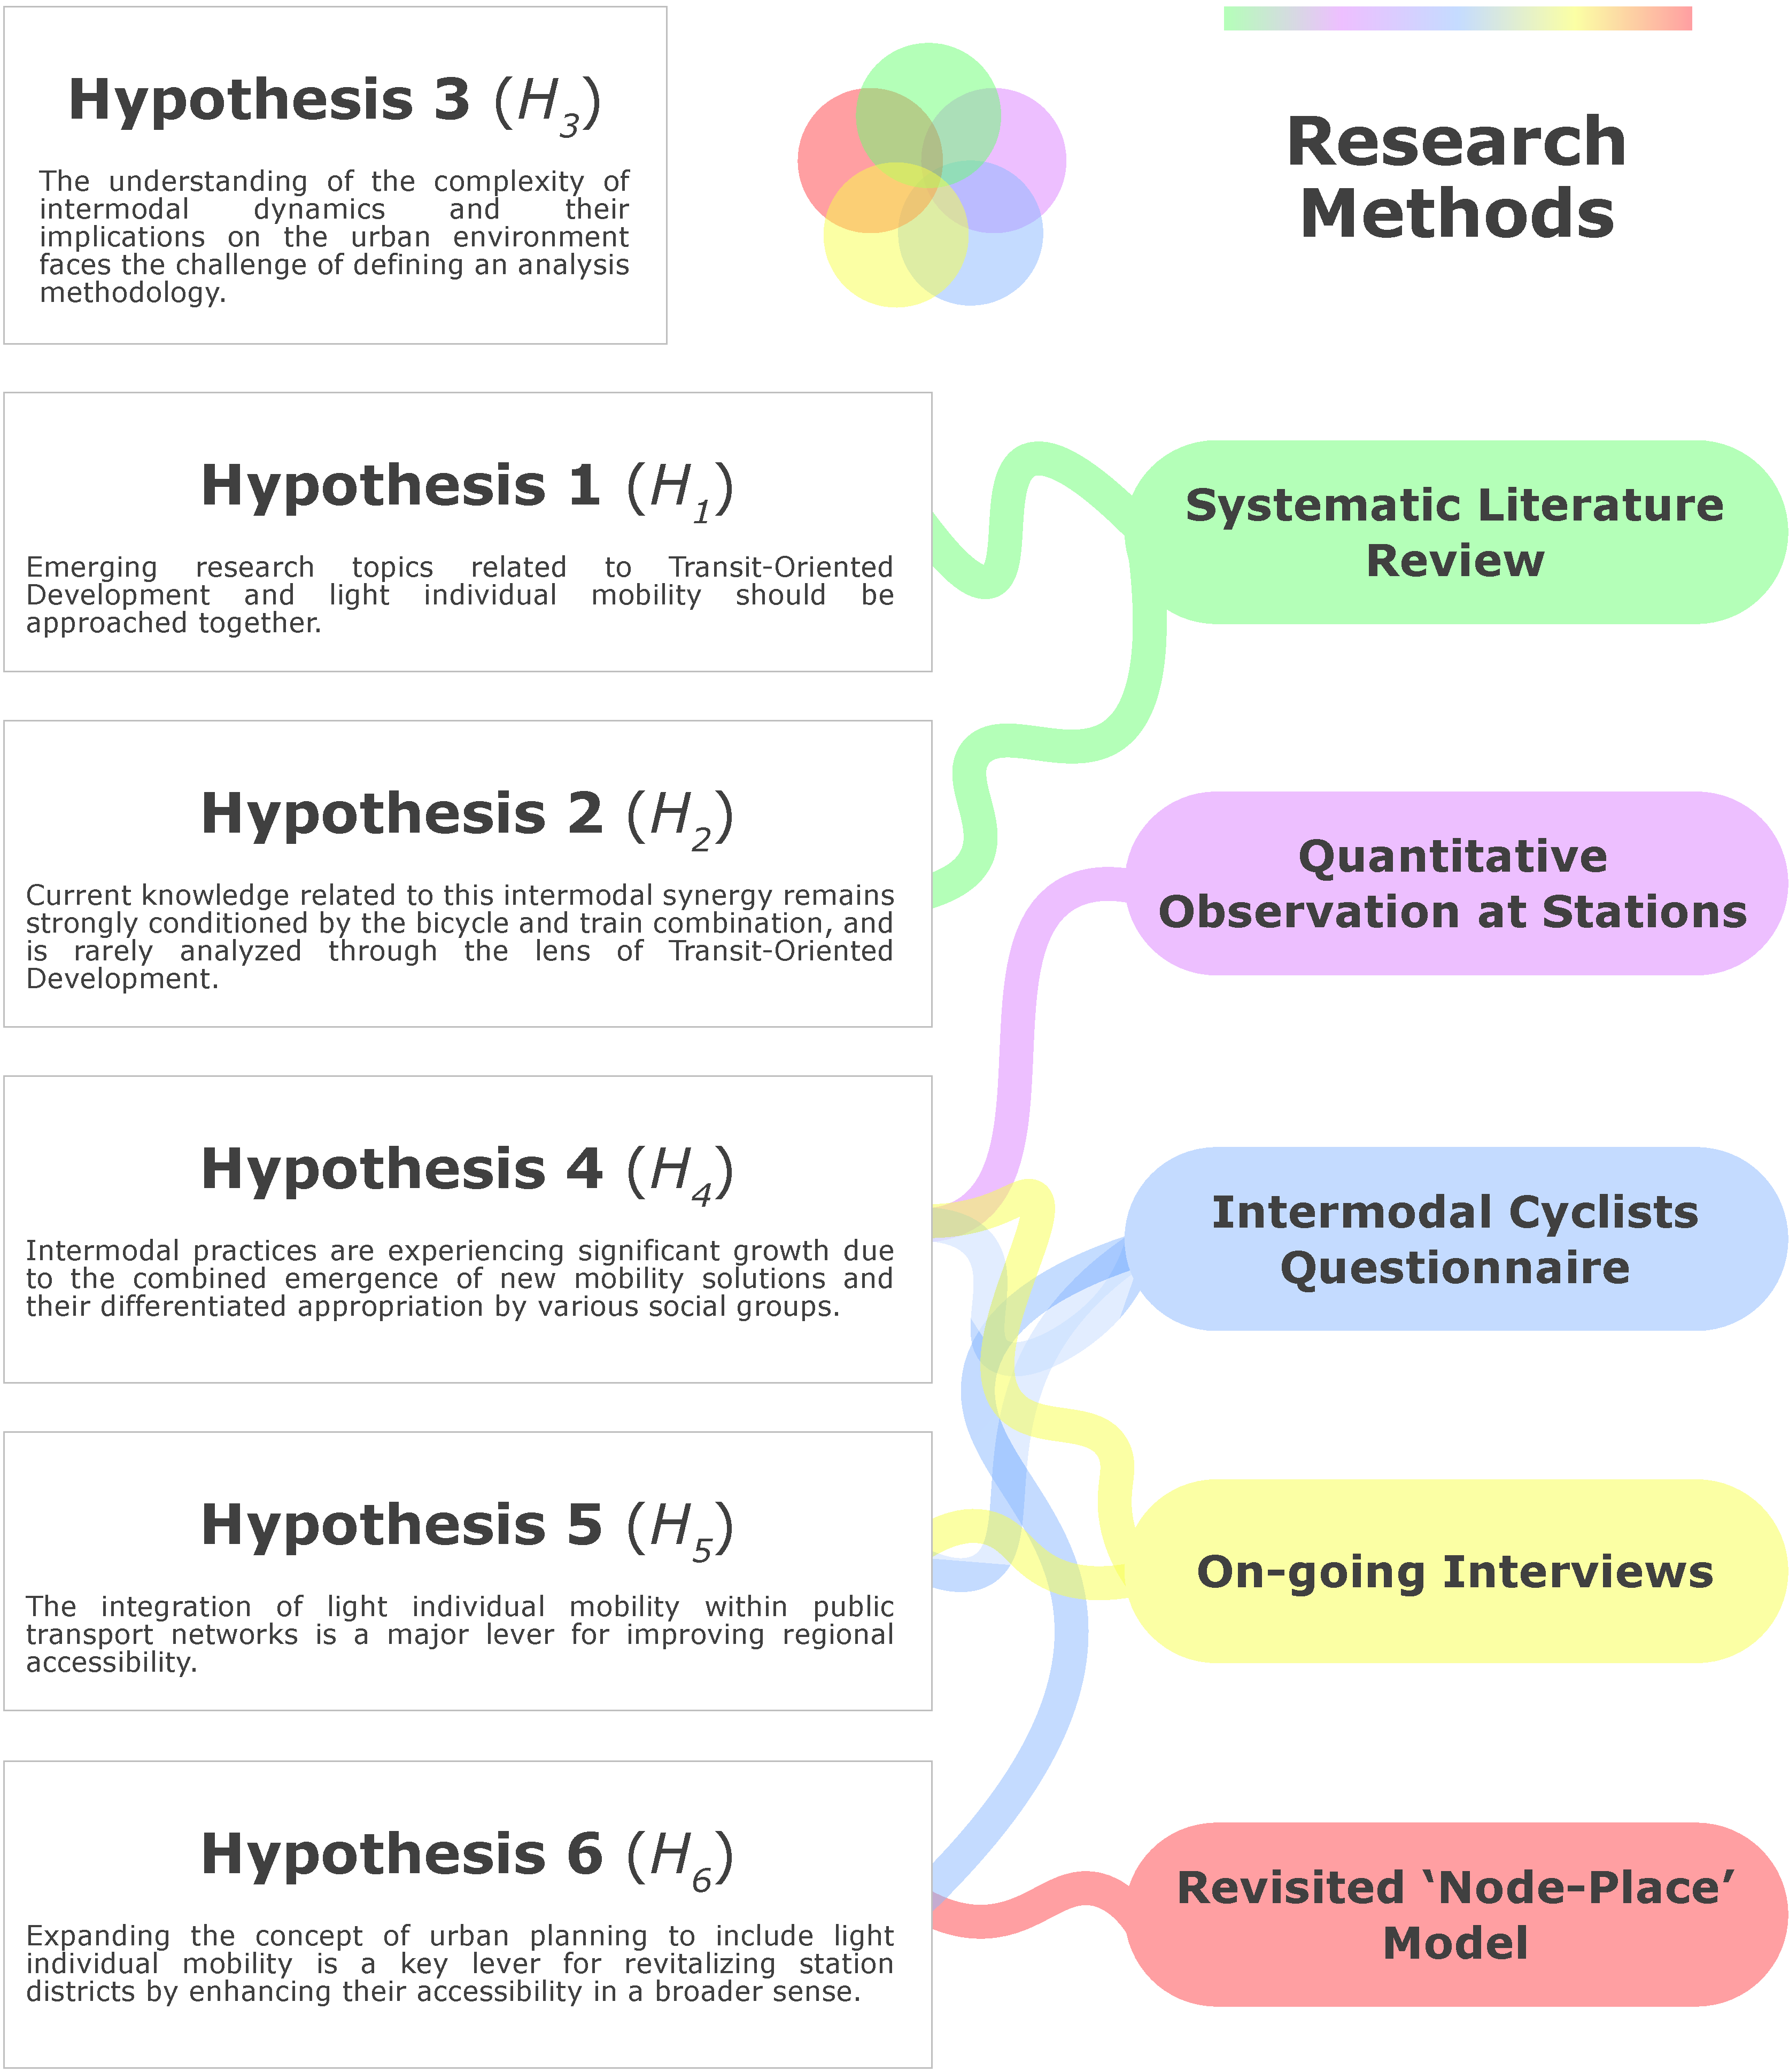
\includegraphics[width=1\columnwidth]{src/Figures/Introduction/EN_Methodologie_hypotheses.pdf}}
        \vspace{5pt}
        \begin{flushright}\scriptsize{
        Author~: \textcolor{blue}{Dylan Moinse (2025)}
        }\end{flushright}
    \end{figure}

% Methodology
The chosen methodology is primarily based on the need to synthesize existing works and knowledge related to the research problem. To this end, a \acrfull{SLR} was conducted on studies related to the contours of \acrshort{B-TOD} and \acrshort{M-TOD}, in line with \hyperref[hypothese-1]{hypotheses~\(H_1\)} and \hyperref[hypothese-2]{\(H_2\)} (page~\pageref{hypothese-2}). This is followed by field exploration in the form of a quantitative observation, aimed at characterizing the emerging phenomenon of nodal connection facilitated by light individual mobility, in accordance with \hyperref[hypothese-4]{hypothesis~\(H_4\)} (page~\pageref{hypothese-4}). This survey is complemented by conducting mobile interviews, with a guided route, enriching the investigation by accessing the \gls{perception} of users and refining the understanding of their intermodal practices. A third type of survey involves a questionnaire addressed to cycling passengers, intended to represent intermodal travel in order to identify the territories frequented and experienced near exchange hubs, continuing from \hyperref[hypothese-5]{hypothesis~\(H_5\)} (page~\pageref{hypothese-5}). Finally, spatial modeling has been undertaken to revisit the \textquote{node-place} tool, commonly applied in \acrshort{TOD} studies. This modeling allows for capturing the implications of integrating light individual mobility and identifying its interactions with the urban environment, supported by \hyperref[hypothese-6]{hypothesis~\(H_6\)} (page~\pageref{hypothese-6}).%%Translated%%

% --- %
    % *.5. Thesis Outline
    \needspace{1\baselineskip} % Reserve space
\section*{Thesis Structure
    \label{introduction-generale:annonce-plan}
    }
    \addcontentsline{toc}{section}{Thesis Structure}
    %\markboth{Thesis Outline}{}
    \markright{Thesis Outline}{}

% Introduction
This thesis is structured into three parts and six chapters, following a logical progression that allows for the exploration of the theoretical foundations, challenges, and implications of integrating light individual mobility into the \acrshort{TOD} model (see the \hyperref[fig-introduction:structure-these]{diagram~\ref{fig-introduction:structure-these}}, page~\pageref{fig-introduction:structure-these}). Alternating between conceptual approach, state of the art, methodological framework, empirical study, and prospective modeling, it leads to the proposal of a renewed model: an \acrfull{M-TOD}. The argument developed is based on three main axes: (i) a deep understanding of the uses and behaviors related to light individual mobility from an intermodal perspective; (ii) a multi-criteria analysis of the potential for accommodating territories based on their capacity to integrate these new forms of mobility; and (iii) an inquiry into the role of public action in planning and structuring these practices within transport and urban policies. In parallel, three progressive and multiscalar levels of analysis underpin this reflection: (i) examining the dynamics of intermodal demand; (ii) evaluating intermodal accessibility, considered from the perspective of network performance, available resources, time constraints, and individual characteristics; (iii) as well as analyzing the interactions between transport and urban planning in a context of modal integration. The structure of this research, which reflects the scientific approach adopted, can be summarized as follows: \textsl{synthesize and rethink} (see \hyperref[part1:titre]{Part One}, page~\pageref{part1:titre}); \textsl{represent and understand} (see \hyperref[part2:titre]{Part Two}, page~\pageref{part2:titre}); and \textsl{anticipate and guide} (see \hyperref[part3:titre]{Part Three}, page~\pageref{part3:titre}).%%Translated%%

% Figure structure of the thesis
    \begin{figure}[h!]\vspace*{4pt}
        \caption{Overall Structure of the Doctoral Research}
        \label{fig-introduction:structure-these}
        \centerline{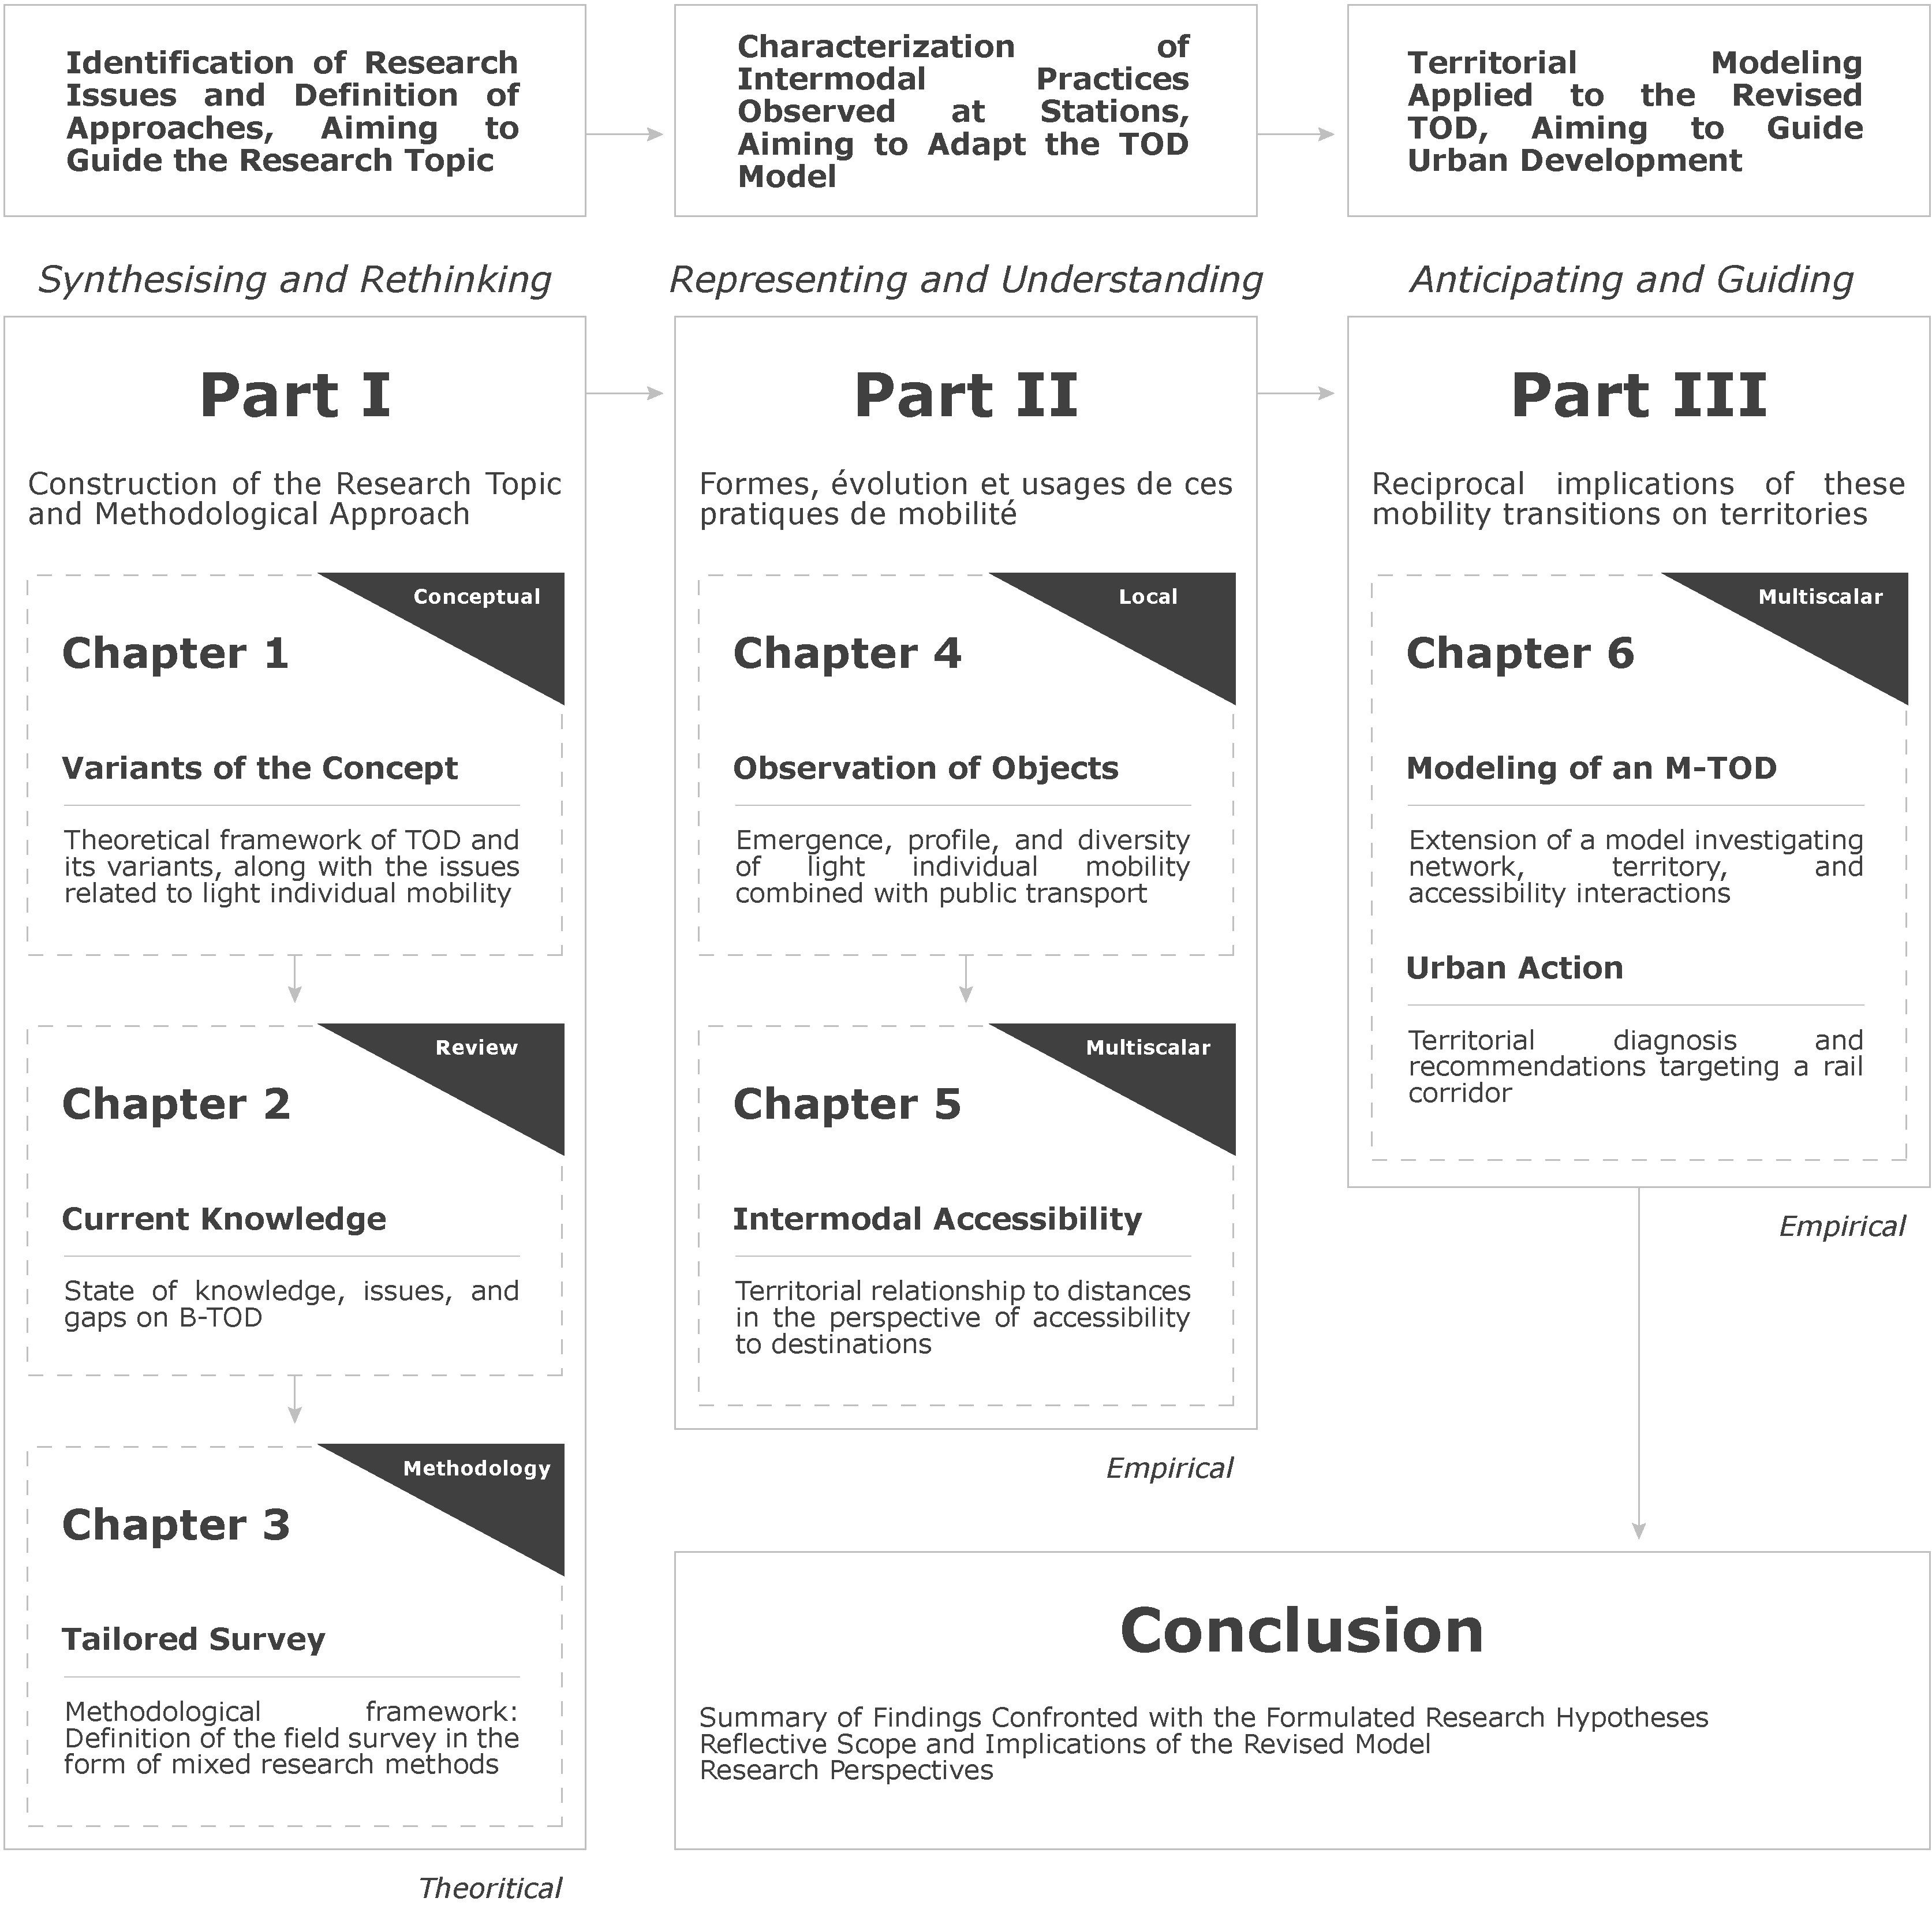
\includegraphics[width=1\columnwidth]{src/Figures/Introduction/EN_Structure_these.pdf}}
        \vspace{5pt}
        \begin{flushright}\scriptsize{
        Author~: \textcolor{blue}{Dylan Moinse (2023)}
        }\end{flushright}
    \end{figure}

% *.5.1. Outline of the plan: part 1
    \needspace{1\baselineskip} % Reserve space
\subsection*{Part One: \textsl{Synthesize and Rethink}
    \label{introduction-generale:annonce-plan-1}
    }

% Chapter 1
\hyperref[chap1:titre]{Chapter One} (page~\pageref{chap1:titre}) lays the theoretical foundations of this research by defining the fundamental concepts that will structure the argument. It first focuses on the founding principles of \acrshort{TOD}, tracing its evolution and various conceptual and operational adaptations. This urban planning model, conceived as an alternative to the car-centered system, aims to structure urbanization around public transport infrastructures. However, its application reveals limitations in certain contexts, particularly in peri-urban areas where access distances to public transport stations constitute a major barrier to its effectiveness. It is from this perspective that the analysis of light individual mobility is positioned, defined here as a set of vehicles including bicycles and their variants, as well as scooters and other means of transport. These solutions emerge as a strategic lever capable of addressing the shortcomings of conventional \acrshort{TOD} by improving accessibility to hubs, in the context of the \textquote{first and last miles} of public transport. This chapter thus explores the rise of cycling in daily mobility and its gradual inclusion in urban planning policies. It then examines the opportunities associated with integrating light individual mobility into \acrshort{TOD} thinking, questioning its implications in terms of geographical proximity and intermodality. Finally, it concludes with a critical review of the literature, highlighting the theoretical gaps and potentials of an expanded model that incorporates these new intersections between mobility and urban planning, which justify the investigation undertaken in this thesis (\hyperref[objectif-1]{objective~\(O_1\)}, page~\pageref{objectif-1}).%%Translated%%

% Chapter 2
\hyperref[chap2:titre]{Chapter Two} (page~\pageref{chap2:titre}) extends the reflection initiated on the evolution of \acrshort{TOD} by delving deeper into the state of knowledge on its adaptations incorporating light individual mobility, particularly \acrshort{B-TOD} and \acrshort{M-TOD}. It provides a state of the art on the interaction between bicycles, micromobility, and public transport, questioning these interactions at the interface of mobility systems and territorial organization. Drawing on a \acrfull{SLR}, this chapter employs a scientometric approach to identify the geographical, temporal, and institutional dynamics structuring these urban planning models. This study supports the recent rise in research dedicated to these themes and the emergence of new methodological tools, particularly the use of \textsl{Big Data} and geostatistical analysis models. It identifies the key urban determinants influencing mobility behaviors and evaluates the accessibility gains induced by integrating light individual mobility into \acrshort{TOD} strategies. Based on these elements, this chapter defines the theoretical and methodological foundations upon which the empirical investigation conducted in the following chapters rests (\hyperref[objectif-2]{objective~\(O_2\)}, page~\pageref{objectif-2}).%%Translated%%

% Chapter 3
\hyperref[chap3:titre]{Chapter Three} (page~\pageref{chap3:titre}) marks the entry into the study field of the thesis by seeking to evaluate the integration of light individual mobility into the urban model. It presents the methodological framework adopted to carry out this investigation. This chapter contributes to a reflection on the epistemological positioning of the research, justifying the adoption of mixed research methods, combining quantitative and qualitative approaches. This methodology allows for understanding the complexity of mobility behaviors as well as their relationships and effects on territorial accessibility, by cross-referencing different sources of information. This approach, describing the methodological choices, data collection and processing tools, and the construction of the study areas, lays the analytical foundation that guides the interpretation of the results in the following sections (\hyperref[objectif-3]{objective~\(O_3\)}, page~\pageref{objectif-3}).%%Translated%%

% *.5.2. Outline of the plan: part 2
    \needspace{1\baselineskip} % Reserve space
\subsection*{Part Two: \textsl{Represent and Understand}
    \label{introduction-generale:annonce-plan-2}
    }

% Chapter 4
\hyperref[chap4:titre]{Chapter Four} (page~\pageref{chap4:titre}) constitutes the first phase of the empirical analysis, focusing on the study of intermodal practices associated with light individual mobility, which are found in train station districts. It aims, on the one hand, to quantify the extent of the phenomenon by measuring the modal share of transfer modes in travel chains involving public transport. On the other hand, it seeks to better define the corpus of cycling passengers and identify the key factors influencing their modal choices, considering their individual characteristics, perceptions, and their relationship to the urban environment. This chapter highlights the trade-offs made by users in their daily organization of intermodal travel and emphasizes the role of territorial arrangements as structuring factors of these emerging practices. It identifies the conditions that favor their growth and thus prepares the spatial analysis of the next chapter, questioning the role of accessibility and urban configurations as catalysts for these behaviors (\hyperref[objectif-4]{objective~\(O_4\)}, page~\pageref{objectif-4}).%%Translated%%

% Chapter 5
Based on the exploratory results obtained, \hyperref[chap5:titre]{Chapter Five} (page~\pageref{chap5:titre}) focuses on the accessibility gains generated by these modal synergies. It examines how these intermodal practices transform access to train stations and contribute to the reconfiguration of surrounding districts by redefining the influence areas of transport nodes. The main objective is to assess the contribution of light individual mobility in extending the service areas of public transport stops, as well as the benefits in terms of regional access to destinations. The projection of the routes taken highlights the preferred pathways and the factors influencing these choices. This reflection leads to a renewed interpretation of the functional boundaries of train station districts, showing how the integration of light individual mobility can alter their spatial organization and enhance their attractiveness as strategic locations (\hyperref[objectif-5]{objective~\(O_5\)}, page~\pageref{objectif-5}).%%Translated%%

% *.5.3. Outline of the plan: part 3
    \needspace{1\baselineskip} % Reserve space
\subsection*{Part Three: \textsl{Anticipate and Guide}
    \label{introduction-generale:annonce-plan-3}
    }

% Chapter 6
\hyperref[chap6:titre]{Chapter Six} (page~\pageref{chap6:titre}) proposes a formalization of the \acrshort{M-TOD}, designed as an extension of the \acrshort{TOD} that fully integrates the geographical proximities promised by the combined use of walking and light individual mobility. Based on the insights gained, this chapter engages in modeling the \acrshort{M-TOD}, in order to define its guiding principles, its implementation conditions, and the levers to activate in order to promote its development and maximize its benefits. The proposed modeling particularly allows for predicting the patronage of train stations based on the territorial arrangements of each train station district examined, and the pedestrian and cycling accessibility scales within the regional area studied. A classification of the train stations and their service areas is then established, allowing for the identification of strategic urban hubs with the potential for implementing \acrshort{TOD} and \acrshort{M-TOD}, as well as those for which investments and improvements should be considered to strengthen their role in a global alternative mobility system. Finally, this chapter opens with the production of a territorial diagnosis, formulating a series of strategic recommendations, applied to a case study focusing on a railway corridor (\hyperref[objectif-6]{objective~\(O_6\)}, page~\pageref{objectif-6}).%%Translated%%

    % ___________________________________________
    % Subbibliography
    \newpage
    \sectionheader{Bibliography of Introduction}
    \begingroup
    \renewcommand{\bibfont}{\scriptsize}
\printbibliography[segment=\therefsegment, heading=subbibintoc, title={Bibliography of Introduction}, label=introduction:bibliographie]
    \endgroup
    \end{refsegment}

%% ______________________________ %%
% PART 1

% Introduction PART 1
%------------------------------%
%% ✎ Dylan (V1) %%%%%%%%% ✅ %%
%% ✎ Alain (V2) %%%%%%%%% ✅ %%
%% ✎ Dylan (V3) %%%%%%%%% ✅ %%
%------------------------------%

\afterpage{%
%\afterpage{%

    % Arrière-plan partie I
    \AddToShipoutPictureBG*{%
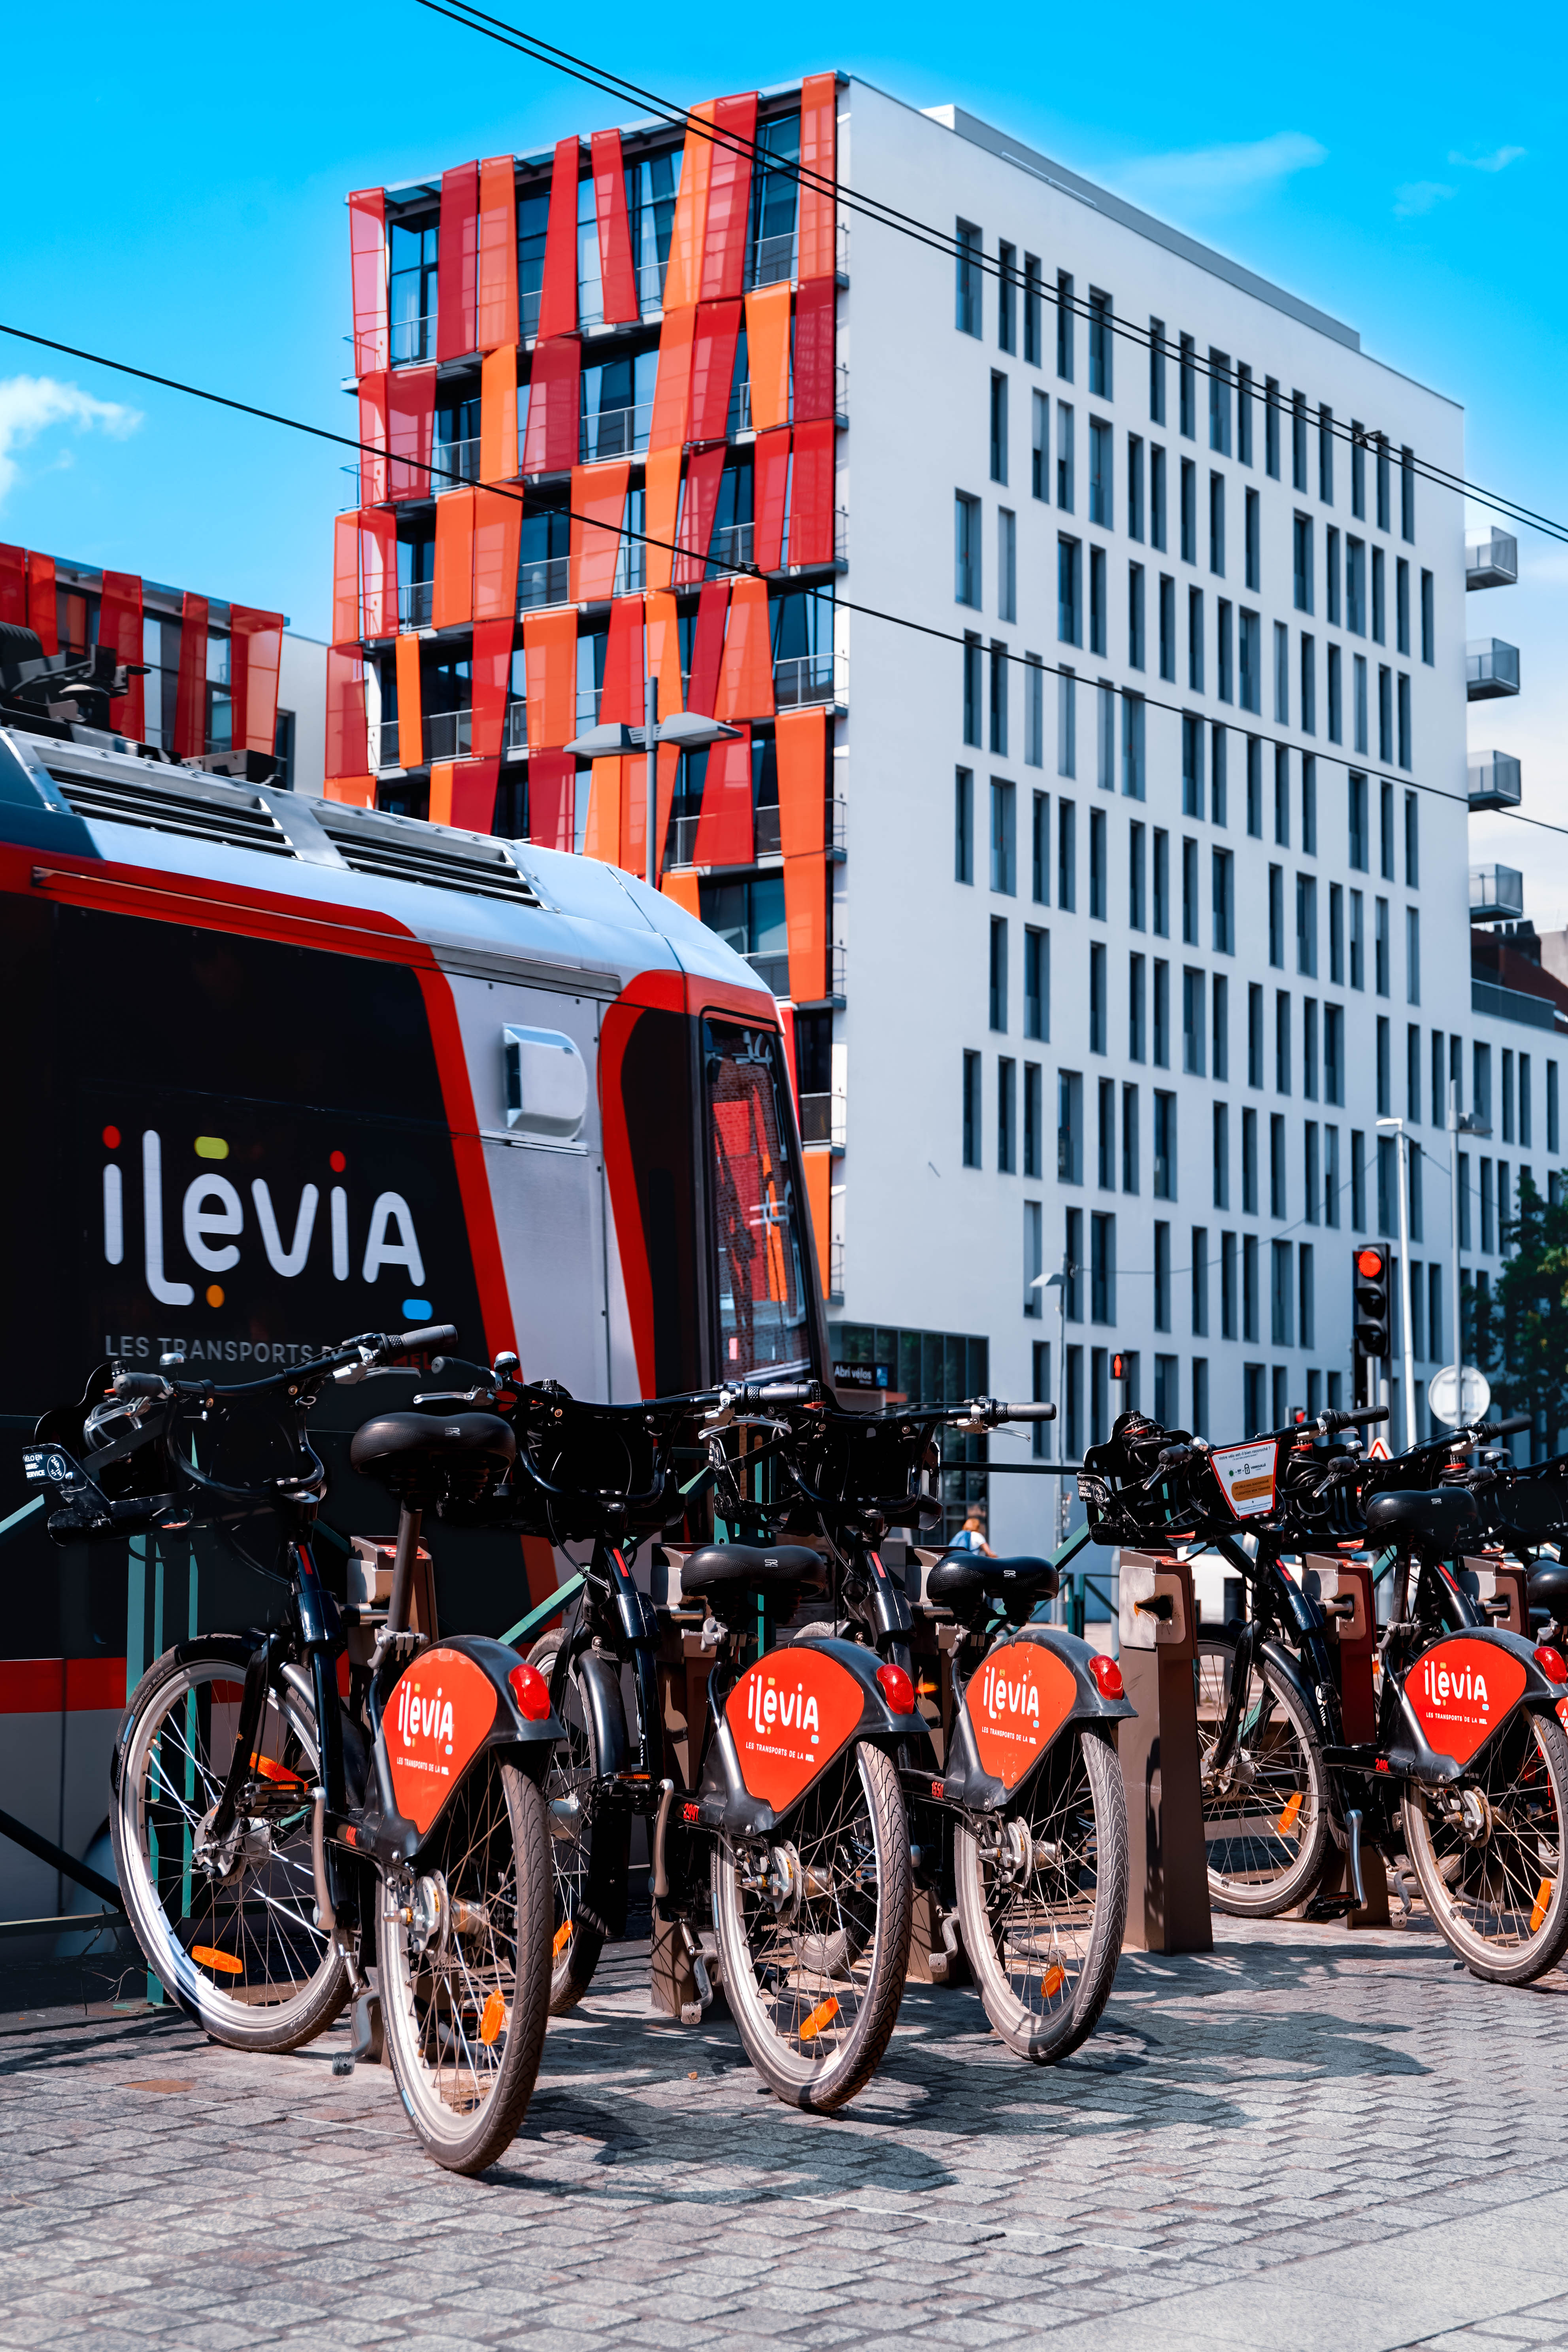
\includegraphics[width=\paperwidth,height=\paperheight]{src/Figures/Arriere_plan/Arriere_plan_Part_1.jpg}
    }

% Rectangle
\AddToShipoutPictureBG*{
  \begin{tikzpicture}[remember picture,overlay]
    \node[fill=white, opacity=0.75, text width=\paperwidth, minimum height=12cm, anchor=north] 
    at ([yshift=-6.7cm]current page.north) {};
  \end{tikzpicture}
}

% Source
\AddToShipoutPictureFG*{
  \AtPageLowerRight{
    \raisebox{1cm}{
      \hspace{16cm}
      
\begin{tikzpicture}
        \node[fill=white, rounded corners=5pt, inner sep=5pt, align=center] {
          \tiny{Photography: \textcolor{blue}{Dylan Moinse (2021)}}
        };
      \end{tikzpicture}
    }
  }
}
}%}

\renewcommand{\thefigure}{\thechapter.\arabic{figure}} % Numérotation standard
\renewcommand{\thetable}{\thechapter.\arabic{table}}
\setcounter{figure}{0}
\setcounter{table}{0}

\needspace{1\baselineskip} % Réserve de l'espace
\part{Theoretical and Methodological Frameworks for Integrating Light Individual Mobility in the Context of Rail-Oriented Urbanism
    \label{part1:titre}
    }
    \markboth{Part~I: Theoretical and Methodological Frameworks of the Research}{}
    \markright{Part~I: Theoretical and Methodological Frameworks of the Research}{}

% Introduction of Part I
\cleardoublepage
\section*{Introduction of Part~I
    \label{part1:introduction}
    }
    \addcontentsline{toc}{chapter}{Introduction of Part~I}

    % Introduction
\lettrine[lines=3, findent=8pt, nindent=0pt]{\lettrinefont T}{he} integration of light individual mobility in station districts and its role in reinterpreting \acrfull{TOD} is part of a broader reflection on the interactions between urbanism, territorial configurations, transport infrastructures, and mobility practices. Before embarking on the construction of empirical data and its analysis, it is essential to revisit the theoretical foundations, conceptual developments, and research methods that will structure this study. This first part thus aims to establish a theoretical and methodological framework that enables understanding the challenges of intermodal accessibility and exploring the ways in which light individual mobility can be integrated into urban planning and transport strategies. It is based on the articulation of three dimensions: (i) a conceptual review of urban models and their adaptation to contemporary mobility dynamics; (ii) a state-of-the-art review of existing research on intermodality and the complementarity between individual mobility and public transport; (iii) a methodological framework detailing the approaches, tools, and analytical techniques used to address these transformations. By gathering these elements, this first part anchors the reflection within a structured framework, justifying the interest of examining \acrshort{TOD} not as a static urban model, but as an evolving strategy capable of integrating light individual mobility to maximize the expected benefits.%%Translated%%

    % Chapter 1
\textsl{Shedding Light on the Conceptual Evolution of Rail-Based Urbanism in View of Its Adjustments} (\hyperref[objectif-1]{Objective~\(O_1\)}, page~\pageref{objectif-1}). \hyperref[chap1:titre]{The first chapter} (page~\pageref{chap1:titre}) traces the evolution of \acrshort{TOD} as a model for structuring regional urban development around public transport networks. It analyzes its core principles, including densification around transport hubs, functional mix, and the treatment of public spaces as tools for creating territories less dependent on automobiles. Despite its ambitions, \acrshort{TOD} presents several structural limitations, particularly in terms of accessibility. While its effectiveness is evident in dense metropolitan contexts, where public transport infrastructures are well integrated into the urban fabric, it proves less effective in suburban areas, where dependence on cars remains prevalent. The main cause lies in the exclusion of intermodal solutions tailored to the \Commas{first and last mile} problem. This situation thus limits the expected positive impacts of \acrshort{TOD} in terms of modal shift and transport network optimization. It is in this context that light individual mobility—including bicycles, scooters, and other micromobility devices, which will also require a reconsideration of their evolution—appears as a strategic lever to complement and update \acrshort{TOD}. Its integration into urban planning and transport policies could help fill the gaps of the traditional model by ensuring a more efficient and alternative mobility system aligned with emerging aspirations. However, this complementarity remains underexplored in academic research and insufficiently implemented in public policies. Once the interest of \acrshort{TOD} as a theoretical framework to address the need for reducing car usage has been demonstrated, its adaptability in areas historically designed for automobiles should be questioned. This reflection thus leads to reviewing the existing literature on this issue and drawing the necessary lessons to guide our own investigation.%%Translated%%

    % Chapter 2
\textsl{Synthesizing Research Practices and Current Knowledge on Public Transport-Oriented Urbanism Supported by Light Individual Mobility} (\hyperref[objectif-2]{Objective~\(O_2\)}, page~\pageref{objectif-2}). \hyperref[chap2:titre]{The second chapter} (page~\pageref{chap2:titre}) constitutes a \acrfull{SLR} designed to better understand the potential synergies between \acrshort{TOD} and light individual mobility. In this context, we use a scientometric approach to identify major research trends related to this topic and to analyze the evolution of associated concepts. This chapter aims to survey and map the works that, implicitly or explicitly, involve the contours of a \acrshort{B-TOD} or \acrshort{M-TOD}. It focuses not only on the geographical and temporal dynamics of publications and their semantics but also on the methods employed in these studies to understand their analytical approaches and underlying methodological frameworks. The analysis of these developments allows for a refined understanding of intermodal mobility practices, incorporating a more nuanced reading of the uses and spatial determinants of intermodal accessibility. Finally, this critical literature review highlights the unresolved challenges, both conceptually and in terms of practical implementation. It raises several key questions for the analyses to come, identifying scientific and methodological gaps that will guide the empirical work of this research. This state-of-the-art review thus serves as a prerequisite for the empirical investigation, building on the gaps identified in the literature to propose a renewed approach capable of better addressing the challenges of \acrshort{M-TOD}.%%Translated%%

    % Chapter 3
\textsl{Developing a Methodology Integrating Complementary Approaches to Achieve a More In-Depth Study and Extract Additional Results} (\hyperref[objectif-3]{Objective~\(O_3\)}, page~\pageref{objectif-3}). \hyperref[chap3:titre]{The third chapter} (page~\pageref{chap3:titre}) addresses the empirical questions raised in the previous chapters. To this end, we have designed and adapted an original methodological framework. This chapter thus presents the methodological approach adopted in this thesis. First, it defines and justifies the choice of the study area, both in terms of the objects analyzed and the geographic area concerned. The construction of our empirical data involves the use of mixed approaches, combining the exploitation of databases, a survey that is both quantitative and qualitative, and spatial modeling. The methodology described allows for the articulation of three complementary levels of analysis: a behavioral level, focusing on modal choices and mobility strategies; an infrastructural level, exploring the physical and organizational conditions of accessibility; and a territorial level, evaluating the potential and actual impact of light individual mobility on station districts. Furthermore, this chapter details the methods used to process the collected data, namely the tools and analytical techniques employed at the interface between geography, sociology, economics, and data science.%%Translated%%

%% ______________________________ %%
% CHAPTER 1
%------------------------------%
%% ✎ Dylan (V1) %%%%%%%%% ✅ %%
%% ✎ Alain (V2) %%%%%%%%% ✅ %%
%% ✎ Dylan (V3) %%%%%%%%% ✅ %%
%------------------------------%

%%%%%%%%%%%%%%%%%%%%%%%%%%%%%%%%
% Chapter~1
\chapterheader{\textsl{Transit-Oriented Development} and Light Individual Mobility}
\chapter
{Challenges and Implications of \textsl{Transit-Oriented Development} Marked by the Rise of Light Individual Mobility
    \label{chap1:titre}
    }
    \begin{refsegment}

    % Background Chapter~1
    \AddToShipoutPictureBG*{%
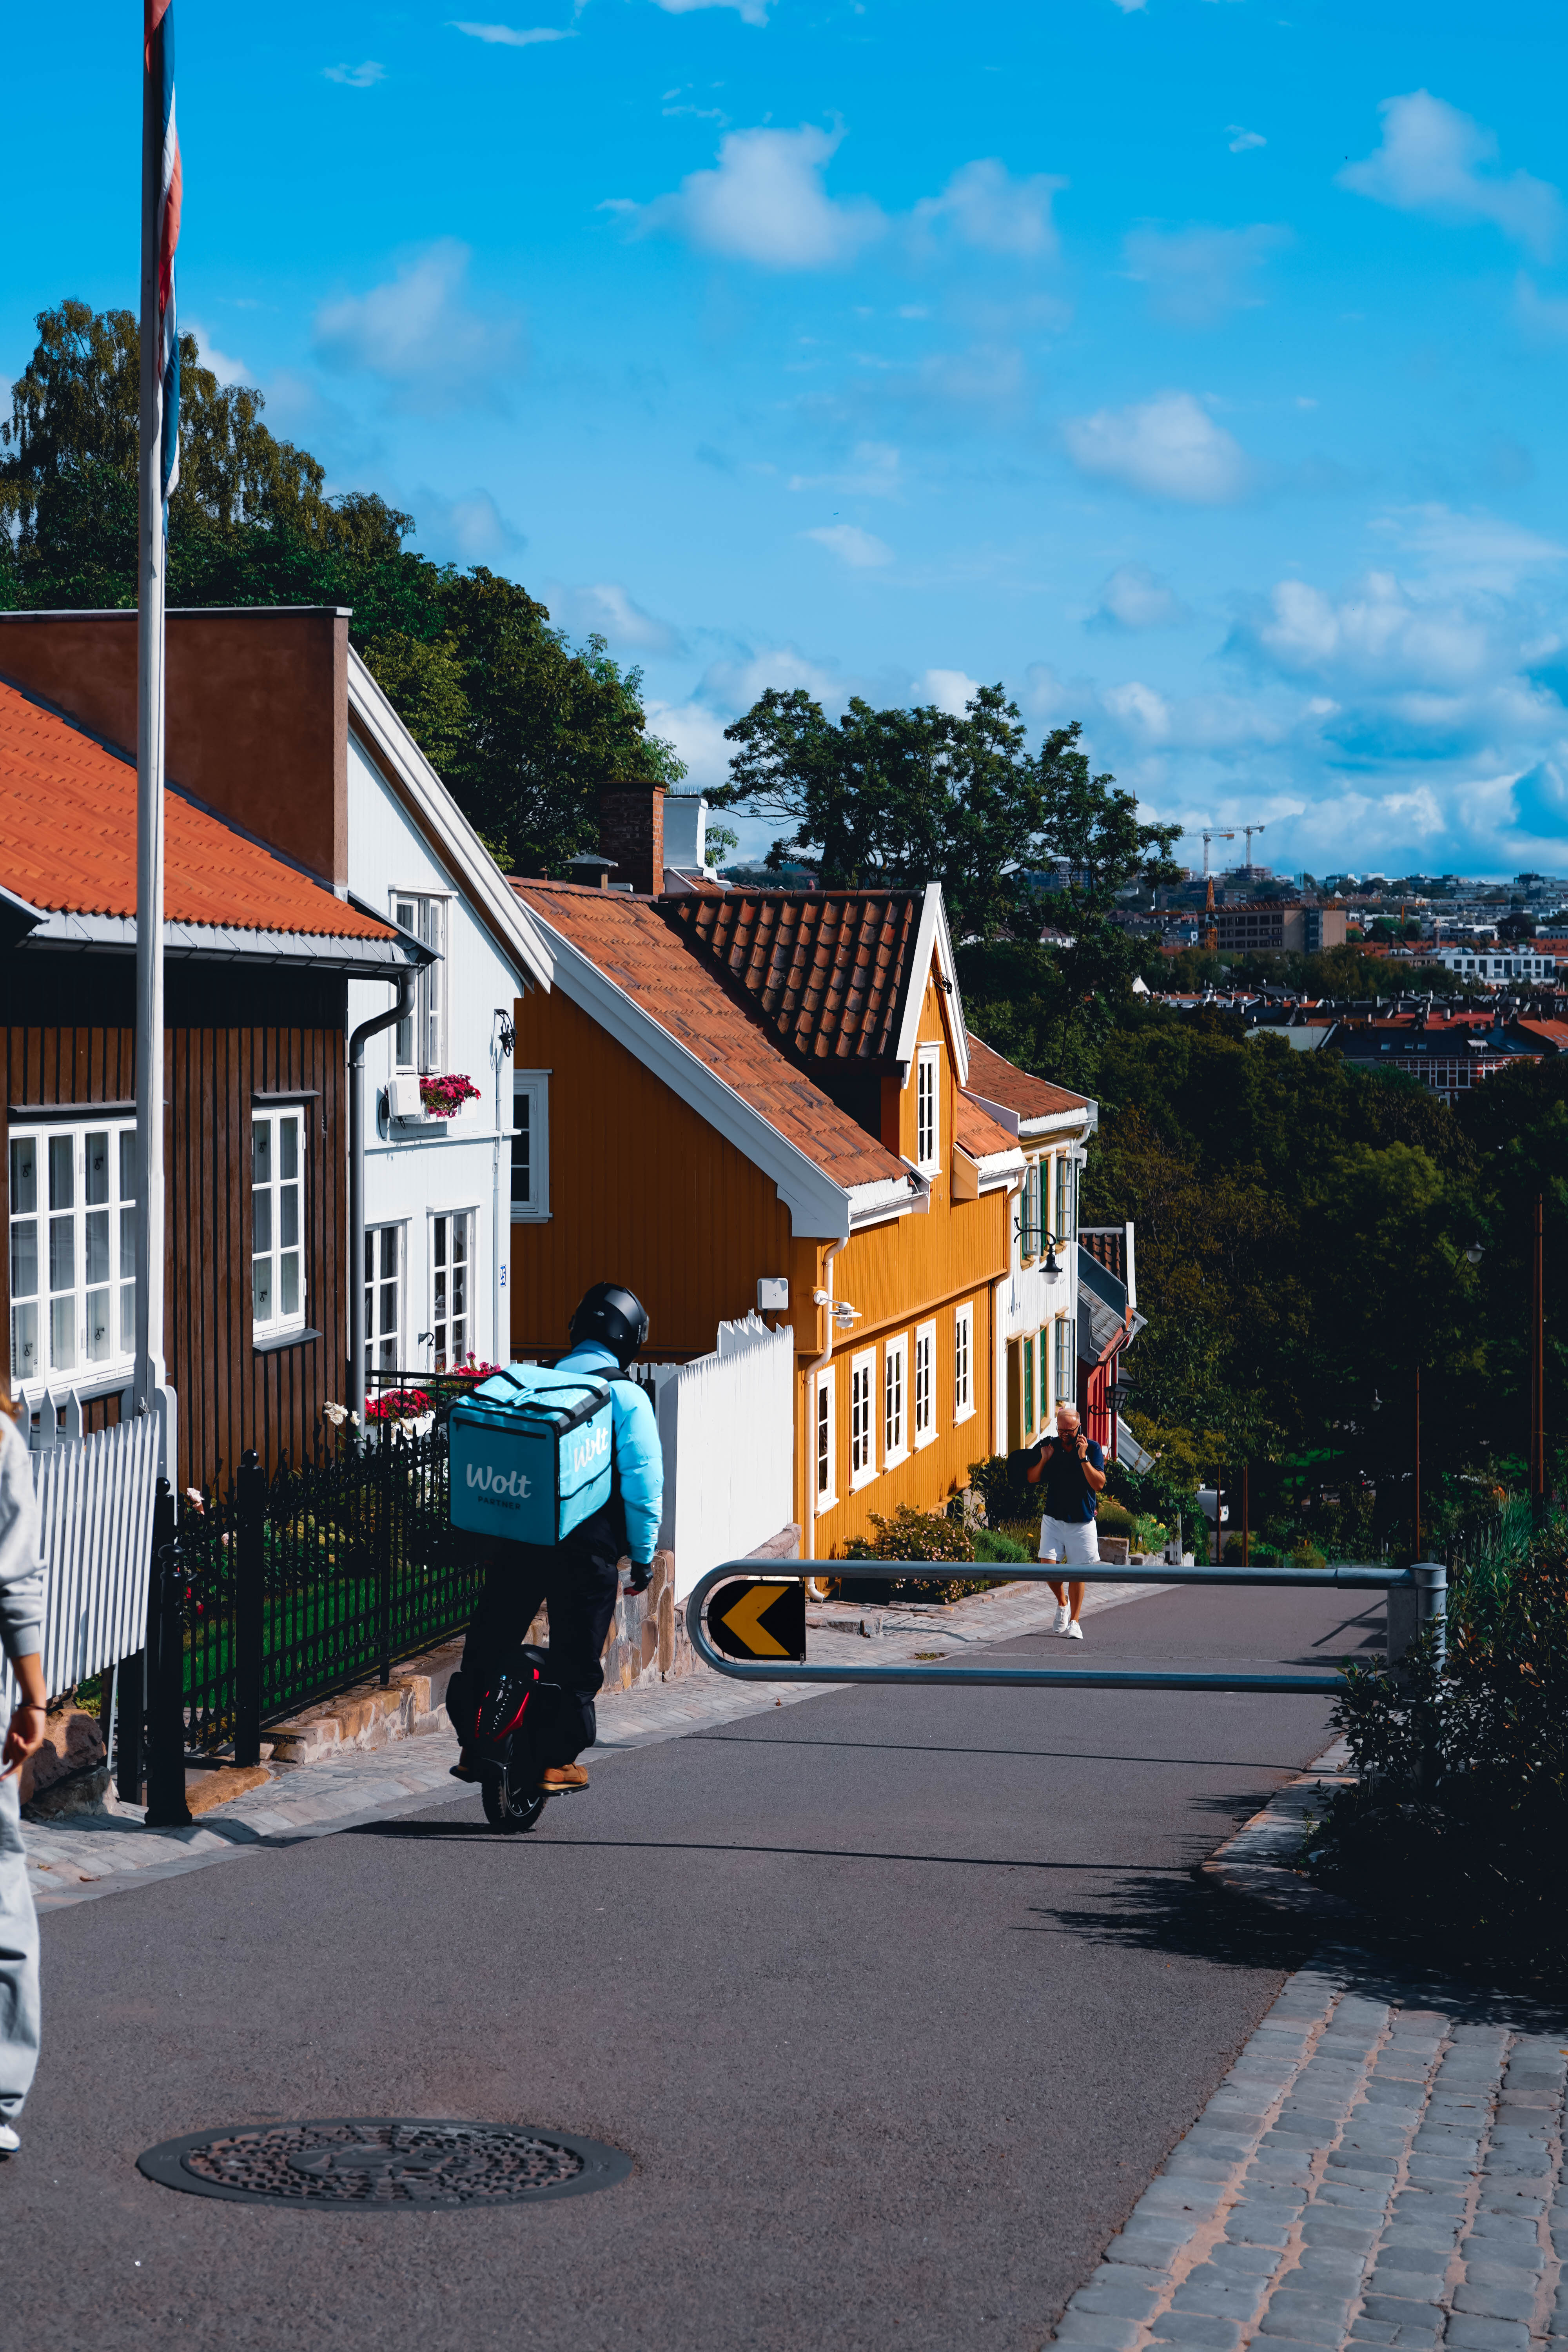
\includegraphics[width=\paperwidth,height=\paperheight]{src/Figures/Arriere_plan/Arriere_plan_Chap_1.jpg}
    }

% Rectangle
\AddToShipoutPictureBG*{
  \begin{tikzpicture}[remember picture,overlay]
    \node[fill=white, opacity=0.75, text width=\paperwidth, minimum height=9.5cm, anchor=north] 
    at ([yshift=-2cm]current page.north) {};
  \end{tikzpicture}
}

% Source
\AddToShipoutPictureFG*{
  \AtPageLowerRight{
    \raisebox{1cm}{
      \hspace{16cm}
      
\begin{tikzpicture}
        \node[fill=white, rounded corners=5pt, inner sep=5pt, align=center] {
          \tiny{Photography: \textcolor{blue}{Dylan Moinse (2023)}}
        };
      \end{tikzpicture}
    }
  }
}

    % ___________________________________________
    % Mini Table of Contents
    \cleardoublepage
    \setcounter{tocdepth}{2}
    % Redefine local table of contents title
    \renewcommand{\localcontentsname}{Table of Contents for Chapter~1}
\localtableofcontents

% Reset section numbering
\setcounter{section}{0}

    % ___________________________________________
    % Graphical Abstract
    \newpage
\section*{Key Points of Chapter~1
    \label{chap1:graphical-abstract}
    }
    \markright{Chapter Preamble}{}

\begin{figure}[h!]\vspace*{4pt}
        \caption*{Theoretical Framework of a \textsl{Micromobility-friendly Transit-Oriented Development}}
        \label{graphical-abstract-chap1}
        \centerline{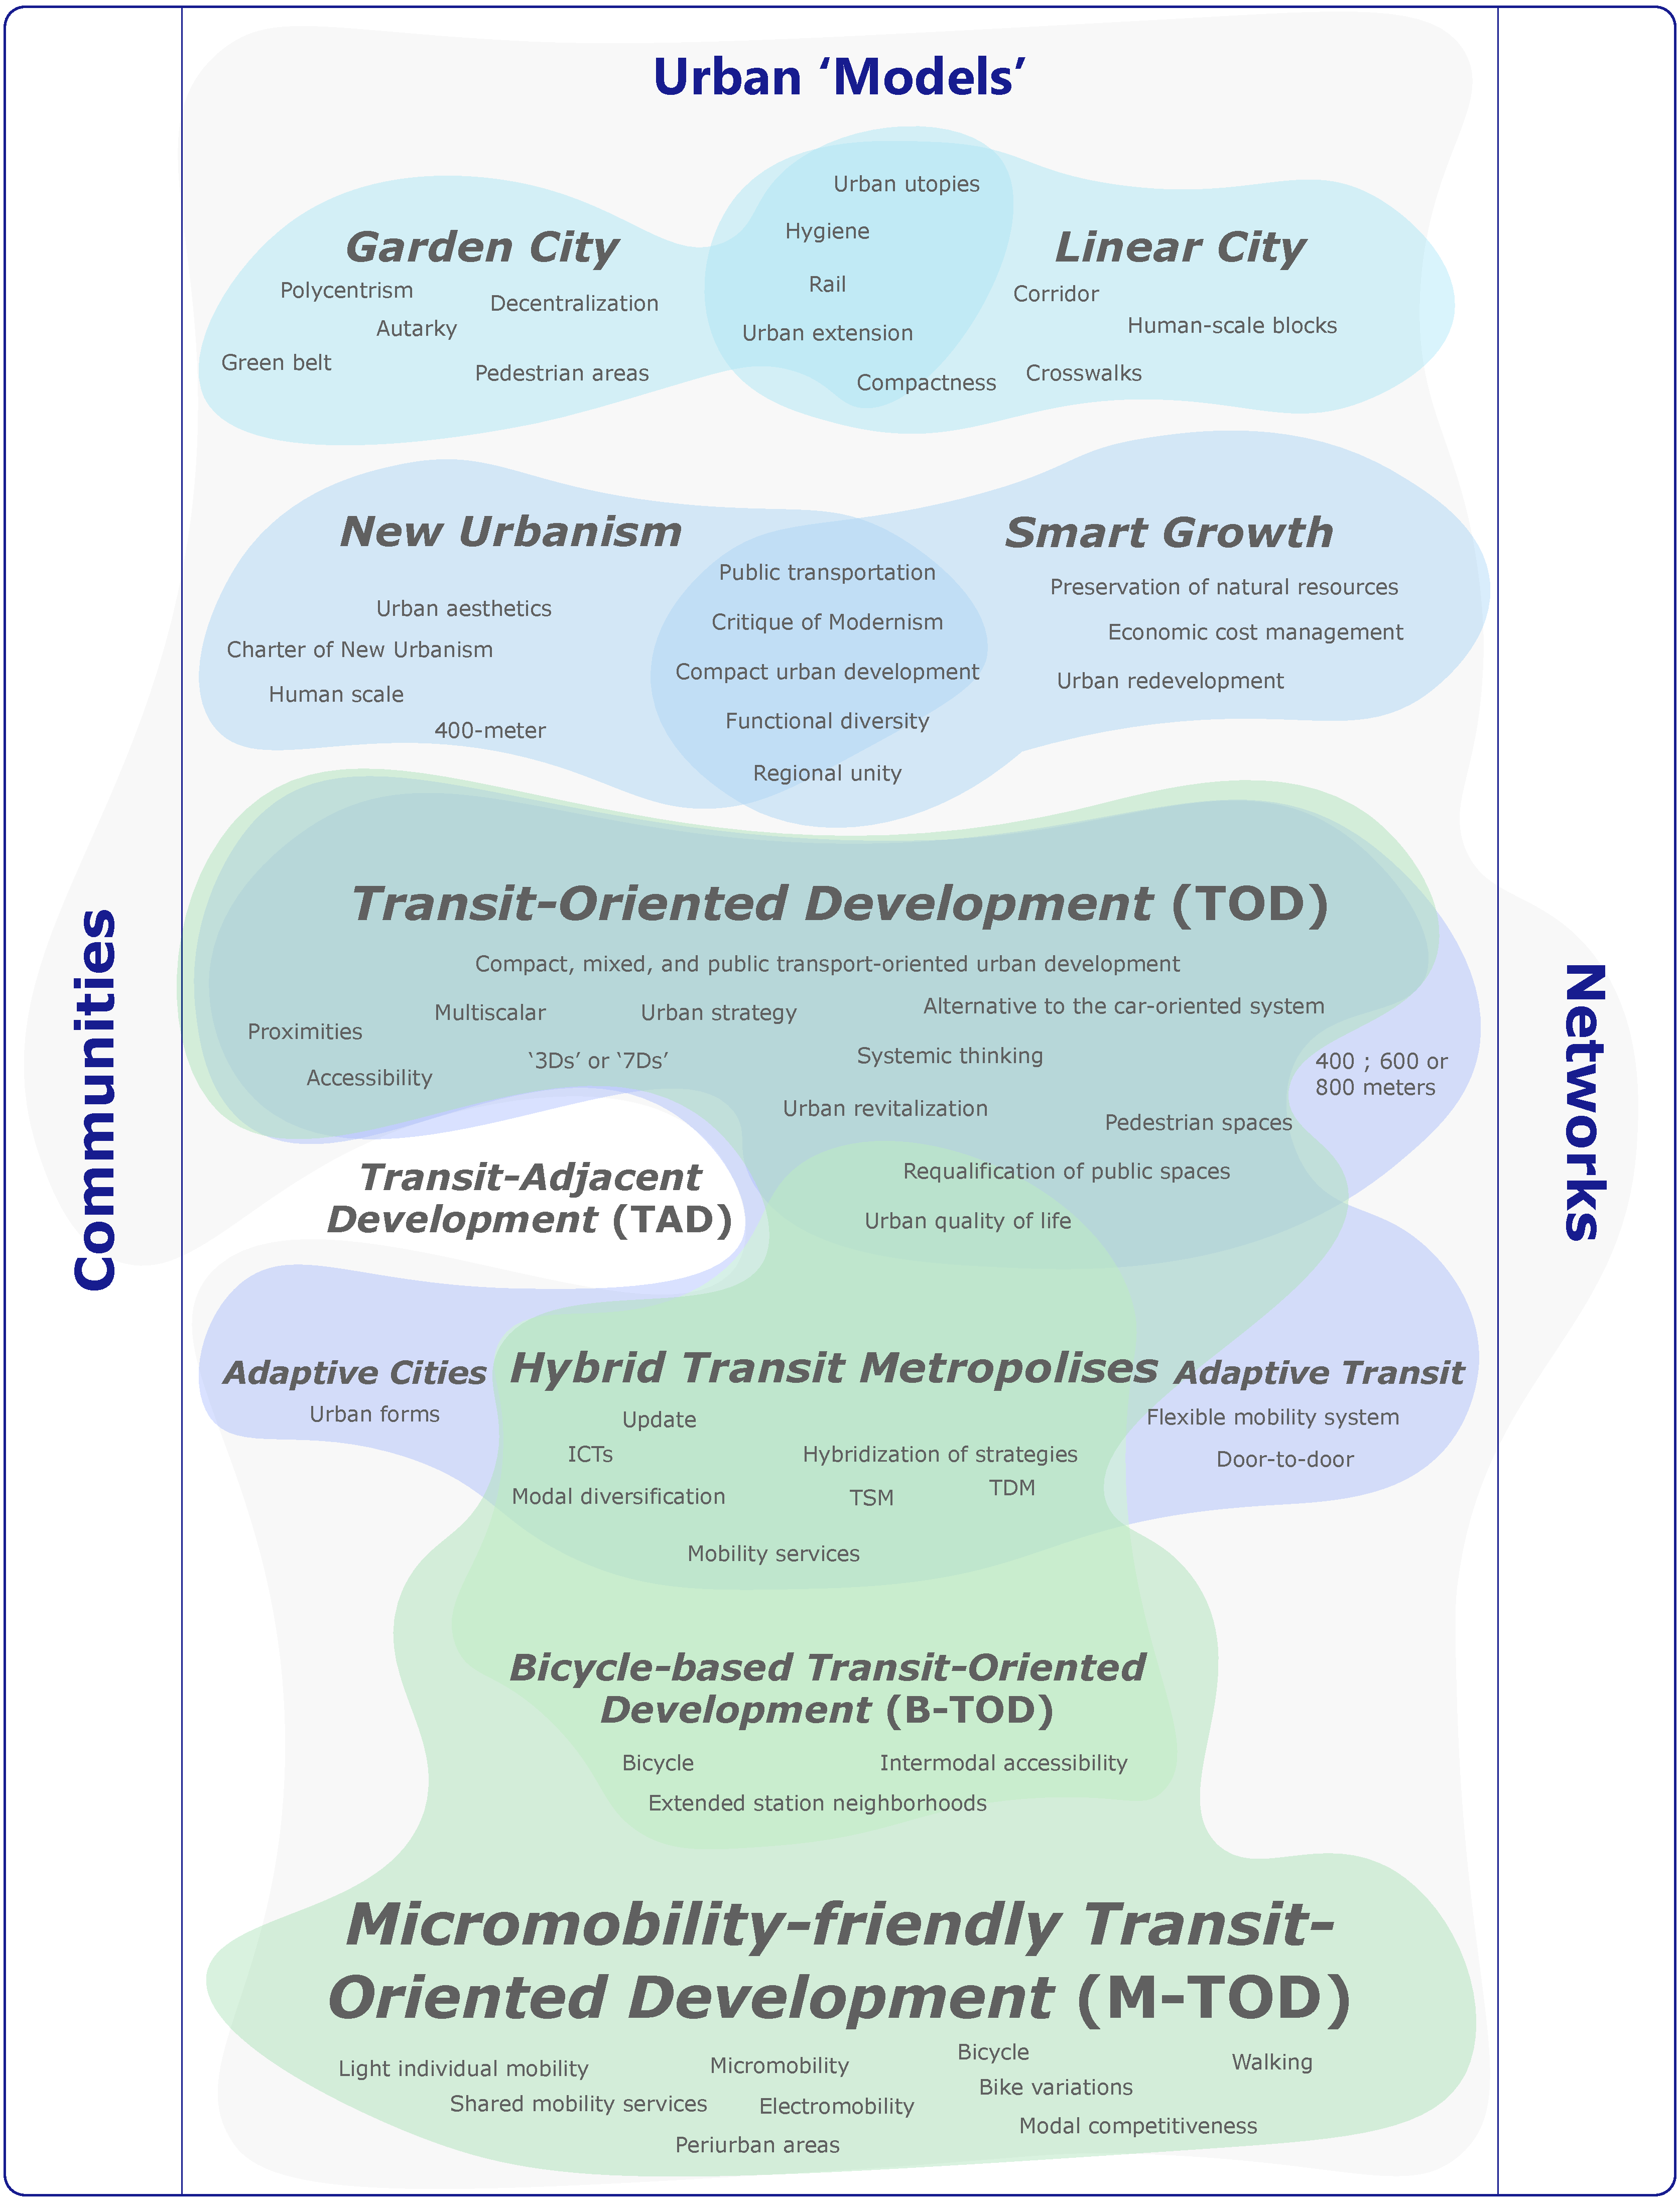
\includegraphics[width=1\columnwidth]{src/Figures/Graphical-abstract/EN_Graphical_abstract_chap1.pdf}}
        \vspace{5pt}
    \end{figure}
    
    % ___________________________________________
    % Preamble
    \newpage
    \begin{tcolorbox}[colback=white!5!white,
                      colframe=blue!75!blue,
                      title=
                      \bigskip
                      \center{\textbf{Preamble of Chapter~1}}
                      \\
                      \raggedright{\small{Chapter composed of \pagedifference{chap1:titre}{chap2:titre} pages, including \pagedifference{chap1:bibliographie}{chap2:titre} pages of bibliography}}
                      \bigskip]
\Large{\textbf{\textcolor{blue}{Abstract:}}}
    \\
    \small{
Formalized in the United States in the 1990s, \acrshort{TOD} represents an urban planning model based on the articulation between densification, functional diversity, public space requalification, and public transport development, with the objective of reducing automobile dependency and fostering a more resilient urban system. This concept follows a lineage of intellectual and urbanistic traditions inherited from several major historical currents. Among them, the \textsl{Garden City} and \textsl{Linear City} introduced planning structured around public transport infrastructures, while \textsl{New Urbanism} and \textsl{Smart Growth} updated these principles to address contemporary urbanization challenges and urban sprawl driven by automobile dominance. \textsl{TOD} thus materializes as an urban strategy aimed at structuring territorial organization \textsl{in connection} with the public transport network, promoting a compact, mixed-use city conducive to alternatives to private cars (see \hyperref[chap1:tod-presentation-generale]{Section~1}, page~\pageref{chap1:tod-presentation-generale}).%%Translated%%
    \\
However, implementing \acrshort{TOD} faces several challenges. While its principles remain particularly relevant for metropolitan areas with a dense and efficient rail network, their transposition to suburban territories encounters significant structural obstacles. The extension of travel distances, the fragmentation of locations, and the intrinsic limitations of public transport networks reduce the model’s effectiveness in such contexts. Furthermore, the rigidity of heavy infrastructures complicates their adaptation to inherited urban forms characterized by low density and high automobile dependence. In this perspective, the rise of light individual mobility—including bicycles, scooters, and other lightweight vehicles—offers a strategic lever to enhance accessibility to public transport stations and strengthen network connectivity. This development relies on a variety of technical, service-based, and social innovations, ranging from electromobility to the mutualization of shared fleets. Thus, integrating these modes could expand the reach of \acrshort{TOD} and maximize its benefits (see \hyperref[chap1:mobilite-individuelle-legere]{Section~2}, page~\pageref{chap1:mobilite-individuelle-legere}).%%Translated%%
    \\
This chapter explores, from a theoretical perspective, the potential of light individual mobility as a response to the limitations of \textsl{Transit-Oriented Development} (\acrshort{TOD}). By facilitating \Commas{first and last mile} travel, this category of alternative vehicles optimizes the use of public transport infrastructures while reducing dependence on private cars. Rather than replacing public transport, it follows a complementary intermodal logic, fostering a seamless integration within mobility systems. The evolution of travel practices and the rise of these (new) modes are transforming the relationship between public transport and urban planning, calling for a reinterpretation of established models. This is why we propose expanding the concept of \acrshort{TOD} into an updated urban model, which we refer to as \acrshort{M-TOD}, drawing inspiration from the principles of \acrshort{B-TOD} (see \hyperref[chap1:btod]{Section~3}, page~\pageref{chap1:btod}).%%Translated%%
    }
    \tcblower
\Large{\textcolor{blue}{\textbf{Keywords:}}}
    \\
    \small{
\textsl{Bicycle-based Transit-Oriented Development};
Electromobility;
Modal Hybridization;
\textsl{Hybrid Transit Metropolis};
Innovation;
Light Individual Mobility;
Shared Mobility;
\textsl{Transit-Oriented Development}
    }
    \end{tcolorbox}

% ___________________________________________
% 1.*.
\newpage
\needspace{1\baselineskip} % Reserve space
\addcontentsline{toc}{section}{Introduction of Chapter~1}
\sectionheader{Introduction of Chapter~1}
\section*{Introduction of Chapter~1
    \label{chap1:introduction}
    }
    \markright{Introduction of Chapter~1}{}

    % Citation
\begin{displayquote}
\Commas{\textsl{The} [\textsl{Transit-Oriented Development}] \textsl{model presented in this book} [\dots] \textsl{focus on transit and is meant to broden a larger movement~–~Neo-Traditional Planning and the New Urbanism~–~which has many dimensions and differing emphasis. These approaches share fundamental principles but set out in slightly different directions.} [\dots] \textsl{With regards to all these proposals, it is important to remember that there is no absolute template and that the specifics of place, economics, and politics will always color and balance the different directions.}}

\textcolor{blue}{Peter} \textcolor{blue}{\textcite[10-11]{calthorpe_next_1993}}\index{Calthorpe, Peter|pagebf}. \foreignlanguage{english}{\textsl{The Next American Metropolis: Ecology, Community, and the American Dream}}, Princeton Architectural Press, New York, 175~p. ISBN: \href{https://search.worldcat.org/fr/title/27814585}{1-878271-68-7}
    \end{displayquote}

% Introduction
\lettrine[lines=3, findent=8pt, nindent=0pt]{\lettrinefont F}{acing} the challenges of pollution, urban fragmentation, and congestion caused by the widespread use of automobiles and urbanization adapted to this mode of transportation, the concept of \acrfull{TOD} planning is based on the principle of densification and diversification of activities and uses around public \gls{public transport} infrastructure. Formalized in the United States under the impetus of \textcolor{blue}{Peter} \textcolor{blue}{\textcite[10]{calthorpe_next_1993}}\index{Calthorpe, Peter|pagebf}, this urban model draws from several schools of thought, notably the \textsl{Garden City} of \textcolor{blue}{Ebenezer} \textcolor{blue}{\textcite{howard_-morrow_1898}}\index{Howard, Ebenezer|pagebf}, the \textsl{Linear City} of \textcolor{blue}{Arturo Soria y Mata (1882)}, as well as the principles of \textsl{New Urbanism} and \textsl{Smart Growth}. A fundamental element of \acrshort{TOD} lies in its ability to explicitly articulate public transport and urban planning in a synergistic manner, far beyond a simple juxtaposition of infrastructure and activities. It is a multidimensional and multiscale approach where the public transport station becomes the structuring pivot of the territory. In this logic, the nodal point no longer merely connects flows but genuinely interacts with them by connecting to the place \textcolor{blue}{\autocite[344]{bertolini_nodes_1996}}\index{Bertolini, Luca|pagebf}, based on a \Commas{place-movement} approach \textcolor{blue}{\autocite[103]{le_bot_flux_2024}}\index{Le Bot, Nils|pagebf}. This model aims to promote a more compact and lively urbanism to better control urban sprawl and encourage travel by public transport, as well as on foot and by \gls{bicycle}. Moreover, it contributes to the reorganization of activities at the territorial scale by promoting a polycentric structure \textcolor{blue}{\autocite[38]{pearce_enquete_2020}}\index{Pearce, Marc|pagebf}\index{Landriève, Sylvie|pagebf}\index{Gay, Christophe|pagebf}\index{Dubois, Tom|pagebf}, in the manner of a \Commas{centralized decentralization} \textcolor{blue}{\autocite[55]{kamruzzaman_advance_2014}}\index{Kamruzzaman, Md.|pagebf}\index{Baker, Douglas|pagebf}\index{Washington, Simon|pagebf}\index{Turrell, Gavin|pagebf}. Today, \acrshort{TOD} is emerging as one of the urban strategies closest to what we can qualify as \Commas{sustainable urbanism} or \Commas{sustainable urban development} \textcolor{blue}{\autocite[14]{bentayou_transit-oriented_2015}}\index{Bentayou, Gilles|pagebf}. Furthermore, the latest report from the \acrfull{IPCC} recommends urban development oriented towards public transport networks and active modes, designed to promote urban compactness \textcolor{blue}{\autocite[29]{lee_climate_2023}}\index{Lee, Hoesung|pagebf}\index{Calvin, Katherine|pagebf}\index{Dasgupta, Dipak|pagebf}\index{Krinner, Gerhard|pagebf}\index{Mukherji, Aditi|pagebf}\index{Thorne, Peter|pagebf}\index{Trisos, Christopher|pagebf}\index{Romero, Jose|pagebf}\index{Aldunce, Paulina|pagebf}\index{Barrett, Ko|pagebf}\index{Blanco, Gabriel|pagebf}\index{Cheung, William|pagebf}\index{Connors, Sarah|pagebf}\index{Denton, Fatima|pagebf}\index{Diongue Niang, Aïda|pagebf}\index{Dodman, David|pagebf}\index{Garschagen, Matthias|pagebf}\index{Geden, Oliver|pagebf}\index{Hayward, Bronwyn|pagebf}\index{|pagebf}\index{Jones, Christopher|pagebf}\index{Frank, Jotzo|pagebf}\index{Thelma, Krug|pagebf}\index{Laco, Rodel|pagebf}\index{Lee, June-Yi|pagebf}\index{Masson-Delmotte, Valérie|pagebf}\index{Meinshausen, Malte|pagebf}\index{Mintenbeck, Katja|pagebf}\index{Mokssit, Abdalah|pagebf}\index{Otto, Friederike~E.~L.|pagebf}\index{Pathak, Minal|pagebf}\index{Pirani, Anna|pagebf}\index{Poloczanska, Elvira|pagebf}\index{Pörtner, Hans-Otto|pagebf}\index{Revi, Aromar|pagebf}\index{Roberts, Debra~C.|pagebf}\index{Roy, Joyashree|pagebf}\index{Ruane, Alex~C.|pagebf}\index{Skea, Jim|pagebf}\index{Shukla, Priyadarshi~R.|pagebf}\index{Slade, Raphael|pagebf}\index{Slangen, Aimée|pagebf}\index{Sokona, Youba|pagebf}\index{Sörensson, Anna~A.|pagebf}\index{Tignor, Melinda|pagebf}\index{Vuuren, Detlef~van.|pagebf}\index{Wei, Yi-Ming|pagebf}\index{Winkler, Harald|pagebf}\index{Zhai, Panmao|pagebf}\index{Zommers, Zinta|pagebf}.%%Translated%%

% Limites et intermodalité
However, the lengthening of distances and the fragmentation of production, consumption, and residential areas, resulting from functional zoning and the horizontal artificialization of soils, have significantly reduced the attractiveness and competitiveness of public transport across a large part of the territories \textcolor{blue}{\autocite[25-28]{mallet_voyage_2022}}\index{Mallet, Thierry|pagebf}. Moreover, the public transport system fails to match all the benefits provided by car use, particularly in terms of flexibility and connectivity \textcolor{blue}{\autocite[209]{heran_retour_2015}}\index{Héran, Frédéric|pagebf}. This situation thus questions the ability of the urban model to effectively address car dependency, especially in peri-urban areas. An alternative lies in promoting intermodality, which could mitigate the rigidity of the public transport network \textcolor{blue}{\autocite[17]{wiel_comment_1998}}\index{Wiel, Marc|pagebf} and improve the overall efficiency of the mobility system \textcolor{blue}{\autocite[82]{oostendorp_combining_2018}}\index{Oostendorp, Rebekka|pagebf}\index{Gebhardt, Laura|pagebf}. By moving beyond strictly monoscalar and monomodal approaches, corrective measures can be implemented to limit dysfunctions and optimize the performance of intermodal chains, from the regional to the intra-urban scale \textcolor{blue}{\autocite[111-115]{chapelon_transports_2016}}\index{Chapelon, Laurent|pagebf}. The goal is to design an integrated and coherent system where urban growth adapts to the development of public transport as much as alternative mobility solutions adjust to the specificities of the existing urban fabric. Empirically, this approach translates into adopting urban planning strategies that foster a dialogue between transport supply and demand, integrating complementary mobility solutions within a global rather than sectorized system. It is within this perspective that contemporary \textsl{Transit Metropolises} have developed, aiming to compete with the car by mimicking its \Commas{door-to-door} connectivity while adhering to a collective travel logic \textcolor{blue}{\autocite[132-133]{cervero_transit_2020}}\index{Cervero, Robert|pagebf}.%%Translated%%

% Mobilité individuelle légère
In this context, the rise of what we have chosen to call \Commas{light individual mobility}—including bicycles, scooters, and their various adaptations—opens new perspectives for sustainable urban planning and mobility. These solutions offer interesting alternatives to the challenges posed by the \Commas{first and last mile} of public transport and thus emerge as an essential missing link in the transition towards \Commas{ecomobile} mobility \textcolor{blue}{\autocites[4]{sebban_complementarite_2003}[25]{amar_homo_2016}{heran_transition_2018}}\index{Sebban, Annie-Claude|pagebf}\index{Motte, Alain|pagebf}\index{Héran, Frédéric|pagebf}\index{Amar, Georges|pagebf}. Light individual mobility is part of an \Commas{innovative rewriting of the past}, exemplified by the resurgence of bicycles in renewed forms and the rise of scooters as a utilitarian mode of transport \textcolor{blue}{\autocite[18]{amar_homo_2016}}\index{Amar, Georges|pagebf}. The development of these light modes as intermodal solutions reflects a renewal of proximity at various spatial scales \textcolor{blue}{\autocite{sadik-kahn_15-minute_2021}}\index{Sadik-Kahn, Janette|pagebf}, thereby enhancing the attractiveness of public transport and revealing an evolution in mobility values \textcolor{blue}{\autocite[110]{goletz_intermodality_2020}}\index{Goletz, Mirko|pagebf}\index{Haustein, Sonja|pagebf}\index{Wolking, Christina|pagebf}\index{L'Hostis, Alain|pagebf}. Ultimately, the ecomobile city, in contrast to the car-centric city model, relies on local circulation where the complementarity between bicycles and public transport constitutes one of the fundamental principles of a more integrated and resilient mobility system.%%Translated%%

% Annonce du plan 1
This chapter is organized into three main parts exploring the foundations, application, and evolution of \acrshort{TOD}. First, we will examine the origins and theoretical foundations of this urban model by tracing its historical and intellectual influences, as well as its evolution and applicability (\hyperref[chap1:tod-presentation-generale]{Section~1}, page~\pageref{chap1:tod-presentation-generale}). We will analyze the urban planning movements that shaped its formulation and codification before highlighting the unique aspects of \acrshort{TOD} (\hyperref[chap1:tod-presentation-generale-origines]{Subsection~1.1}, page~\pageref{chap1:tod-presentation-generale-origines}). This epistemological retrospective will allow us to precisely define its contours as an alternative urban development model to the car-centric paradigm, specifying its principles and expected benefits (\hyperref[chap1:tod-presentation-generale-definition]{Subsection~1.2}, page~\pageref{chap1:tod-presentation-generale-definition}). Finally, we will see how this planning concept has been interpreted within urban strategies deployed in the French context and its main variations related to our research subject (\hyperref[chap1:tod-presentation-generale-declinaisons]{Subsection~1.3}, page~\pageref{chap1:tod-presentation-generale-declinaisons}).%%Translated%%

% Annonce du plan 2
The second part will focus on the second object of study of this research, namely the family of vehicles grouped under the term \Commas{light individual mobility} (\hyperref[chap1:mobilite-individuelle-legere]{Section~2}, page~\pageref{chap1:mobilite-individuelle-legere}). We will trace the historical evolution of these technical and social objects—notably bicycles and scooters—by identifying and simplifying the reading of the major periods that marked their development, in order to better contextualize their current resurgence of interest (\hyperref[chap1:proximite-velo-trottinette]{Subsection~2.1}, page~\pageref{chap1:proximite-velo-trottinette}). We will then address the diversification of the uses and forms of these vehicles, characterized notably by their electrification and sharing in the \gls{public space}, thereby blurring the traditional boundaries between modes of transport (\hyperref[chap1:velo-micromobilite-innovations]{Subsection~2.2}, page~\pageref{chap1:velo-micromobilite-innovations}). This historical reflection will allow us to expose, in turn, the evolution of values attached to mobility and lifestyles, as well as the definitional challenges related to the scope of relevance of this family of vehicles (\hyperref[chap1:caracterisation-mobilite-individuelle-legere]{Subsection~2.3}, page~\pageref{chap1:caracterisation-mobilite-individuelle-legere}).%%Translated%%

% Annonce du plan 3
Lastly, the third part of this chapter will articulate the previous two by exploring the opportunities offered by the association between public transport and light individual mobility in a modal complementarity logic (\hyperref[chap1:btod]{Section~3}, page~\pageref{chap1:btod}). We will show that, although combined walking is not assimilated to light individual mobility, it remains the structuring element of \acrshort{TOD}. First, we will demonstrate how the real scope of combined walking tends to be underestimated and how light individual mobility can play a complementary role, fitting into a field of relevance that does not compete with walking but reinforces the \gls{accessibility} to public transport (\hyperref[chap1:btod-limites-tod]{Subsection~3.1}, page~\pageref{chap1:btod-limites-tod}). Finally, we will highlight the comparative advantages of such synergy and how this intermodal approach invites us to question the relevance of an expanded model, that of \acrfull{M-TOD} (\hyperref[chap1:btod-m-tod]{Subsection~3.2}, page~\pageref{chap1:btod-m-tod}).%%Translated%%

% ___________________________________________
% 1.1.
\newpage
\needspace{1\baselineskip} % Reserve space
\sectionheader{Concept of \textsl{Transit-Oriented Development}}
\section{Transit-Oriented Development: A Reinvention of Regional Planning Around Railways
    \label{chap1:tod-presentation-generale}
    }

% Introduction TOD
\acrshort{TOD} is now established as a key planning model in regional development, emphasizing rail infrastructure as the central axis of urban growth. This popular strategy is based on the idea of structuring territories around public transport nodes to reduce car dependency and promote more sustainable urbanization. Despite the urgency and importance of these issues, the underlying mechanisms influencing car use in urban environments remain insufficiently understood due to a still limited theoretical framework \textcolor{blue}{\autocite[1]{verbavatz_critical_2019}}\index{Verbavatz, Vincent|pagebf}\index{Barthelemy, Marc|pagebf}. The reflections of Italian architect and urban planner \textcolor{blue}{Alberto} \textcolor{blue}{\textcite[]{magnaghi_bioregion_2014}}\index{Magnaghi, Alberto|pagebf} provide an enriching contribution to this debate by introducing a bioterritorial approach, in which \Commas{urban bioregions} and networks become the pillars of integrated development that respects local ecosystems. However, \acrshort{TOD} stands out as one of the few planning concepts capable of directly addressing and tackling the \Commas{network urbanism} mindset \textcolor{blue}{\autocite[]{dupuy_urbanisme_1991}}\index{Dupuy, Gabriel|pagebf} in a globalized context, highlighting the complex interactions between mobility, urbanization, and sustainability \textcolor{blue}{\autocite[51]{el_hadeuf_ville_2017}}\index{El Hadeuf, Mounya|pagebf}\index{Laterrasse, Jean|pagebf}.%%Translated%%

% Annonce du plan
We will begin by introducing, through a diachronic approach, the origins of the urban model, highlighting the innovative aspects it brings to address contemporary challenges related to the necessary coordination between networks and territories (\hyperref[chap1:tod-presentation-generale-origines]{section on the inspirations of \textsl{Transit-Oriented Development}}, page~\pageref{chap1:tod-presentation-generale-origines}). This introduction will be followed by an overview of the general principles proposed by the planning model to address these issues, as well as the expected effects on territories and mobility behaviors (\hyperref[chap1:tod-presentation-generale-definition]{section on the directions of \textsl{Transit-Oriented Development}}, page~\pageref{chap1:tod-presentation-generale-definition}). Finally, we will pay particular attention to the evolving nature of this concept on a global scale, both in academic and operational settings. We will analyze the various adaptations that result from the specificities of each context and the advancement of knowledge. This reflection will lead us to consider the potential contribution of bicycles and \gls{micromobility} in a perspective of updating the \acrshort{TOD} (\hyperref[chap1:tod-presentation-generale-declinaisons]{section on the main variations of \textsl{Transit-Oriented Development}}, page~\pageref{chap1:tod-presentation-generale-declinaisons}).%%Translated%%

% 1.1.1. Chronologie TOD
\needspace{1\baselineskip} % Reserve space
\subsection{Genesis of \textsl{Transit-Oriented Development}: When Rail Inspires Urbanism
    \label{chap1:tod-presentation-generale-origines}
    }

% Introduction 1
Geography, like many related disciplines, has long emphasized the dynamic interaction between a place and its environment, conceptualizing the place as a \Commas{milieu} that generates activities and drives transformations. By moving beyond the simple notion of physical space, the territorial system acts both as a \textsl{stimulus} and a product of transformations \textcolor{blue}{\autocite[19-21]{hagerstrand_what_1970}}\index{Hägerstrand, Torsten|pagebf}. This approach includes the capacity of train stations, as liminal spaces, to act as catalysts for various developments \textcolor{blue}{\autocite[6]{baron_nouvelle_2024}}\index{Baron, Nacima|pagebf}\index{Le Bot, Nils|pagebf}\index{Detavernier, Pauline|pagebf}. In the 1970s, the \Commas{new geographers} focused their work on the study of networks \textcolor{blue}{\autocites{claval_nouveaux_1977}[166]{massardier_savants_1996}[112-113]{orain_geographie_2006}}\index{Massardier, Gilles|pagebf}\index{Claval, Paul|pagebf}\index{Orain, Olivier|pagebf}, leveraging the dense network of rail infrastructures to analyze reticular forms. These studies explored the reciprocal interactions between networks and territories at various geographical scales \textcolor{blue}{\autocite[6]{baron_nouvelle_2024}}\index{Baron, Nacima|pagebf}\index{Le Bot, Nils|pagebf}\index{Detavernier, Pauline|pagebf}.%%Translated%%

% Introduction 2
In this context, American architect and urban planner \textcolor{blue}{Peter} \textcolor{blue}{\textcite[10]{calthorpe_next_1993}}\index{Calthorpe, Peter|pagebf} proposed a planning model centered on public transport in his work \foreignlanguage{english}{\textsl{The Next American Metropolis: Ecology, Community, and the American Dream}}: the \acrfull{TOD}. This concept asserts itself as a multidimensional action strategy, primarily focused on the physical-spatial aspects of planning \textcolor{blue}{\autocite[10]{calthorpe_next_1993}}\index{Calthorpe, Peter|pagebf}, positing that changes in mobility behavior can stem from urban form. The major influences of \acrshort{TOD} are rooted in the broader framework of \textsl{New Urbanism} and \textsl{Smart Growth}, while introducing a new scale of analysis. Indeed, \textcolor{blue}{Robert} \textcolor{blue}{\textcite[7]{cervero_transit_1998}}\index{Cervero, Robert|pagebf} considers that \acrshort{TOD} shifts the traditional focus from neighborhood or community-level interventions to the connections between public transport and urbanization on a regional scale.%%Translated%%

% 1.1.1.1. Mouvements d'urbanisme
\needspace{1\baselineskip} % Reserve space
\subsubsection*{Legacy of Past Urban Reflections
    \label{chap1:tod-presentation-generale-origines-mouvements}
    }

% Introduction
In her seminal work \textsl{L’urbanisme, utopies et réalités: Une anthologie}, historian \textcolor{blue}{Françoise} \textcolor{blue}{\textcite{choay_urbanisme_1965}}\index{Choay, Françoise|pagebf} provides a framework for understanding the evolution of contemporary cities. According to the author's thesis, the science of urbanism as we know it today does not represent a novel solution to new problems but essentially consists of the reiteration and reproduction of discursive schemas inherited from the 19\textsuperscript{th} century, which she designates as \Commas{models}. This perspective allows us to question the historical and ideological foundations of \acrshort{TOD}. Since the planning concept is rooted in intellectual currents developed in the 1980s in response to the urbanization crisis in the United States and France \textcolor{blue}{\autocite[11]{lefebvre_droit_1967}}\index{Lefebvre, Henri|pagebf}, such as \textsl{New Urbanism} and \textsl{Smart Growth}. However, reducing its inspirations to these postmodern movements would be simplistic. The roots of this model extend to urban theories of the late 19\textsuperscript{th} century, notably the \textsl{Garden City}. \textcolor{blue}{Françoise} \textcolor{blue}{\textcite[259]{choay_urbanisme_1965}}\index{Choay, Françoise|pagebf} identifies the latter as a \Commas{culturalist urbanism}, stemming from a critical theoretical current of the industrial city and characterized by a nostalgic vision of an organic order\footnote{~
    In her typology of \Commas{pre-urbanism} and \Commas{urbanism} movements, \textcolor{blue}{Françoise} \textcolor{blue}{\textcite[277]{choay_urbanisme_1965}}\index{Choay, Françoise|pagebf} designates as \Commas{culturalists} the theoretical currents dating from the second half of the 19\textsuperscript{th} century that advocated for a circumscribed city based on an organic organization, in reaction to the progressive ideas of the time.
}.%%Translated%%

% Cité-jardin : théorie
The \acrshort{TOD} model draws heavily from the concept of the \textsl{Garden City}, originally developed by British urban planner \textcolor{blue}{Ebenezer} \textcolor{blue}{\textcite{howard_-morrow_1898}}\index{Howard, Ebenezer|pagebf}, in reaction to the chaotic urban growth accompanying industrialization in Europe, marked by a lack of urban planning. His thought, formalized in his pamphlet \textsl{Garden Cities of To-Morrow}, characterized by some observers as \Commas{urbaphobic} \textcolor{blue}{\autocite[7]{cavin_cites-jardins_2007}}\index{Cavin, Joëlle Salomon|pagebf}, is based on creating self-sufficient satellite towns on a human scale, embodying the \Commas{fantasy of the dreamed small town} \textcolor{blue}{\autocite[9]{fath_entre_2007}}\index{Fath, Sébastien|pagebf}, combining the advantages of urban and rural life. These towns were designed to be limited in size and extension, connected by rail networks, and organized in a polycentric system with green belts separating each urban center (see \hyperref[fig-chap1:schema-cite-jardin]{Figure~\ref{fig-chap1:schema-cite-jardin}}, page~\pageref{fig-chap1:schema-cite-jardin}). This social project (\textsl{Social City}) aimed to promote a hybrid urbanity oriented towards nature, in contrast to the industrial cities of its time. According to \textcolor{blue}{Robert} \textcolor{blue}{\textcite[38]{fishman_open_2011}}\index{Fishman, Robert|pagebf}, \acrshort{TOD} borrows from garden cities the notions of decentralization and polycentrism, as well as the design of pedestrian-friendly spaces served by railways.%%Translated%%

% Cité-jardin : exemples
Following the success of the first garden city, inaugurated in Letchworth in 1903 and designed by \textcolor{blue}{Ebenezer Howard} \textcolor{blue}{\autocite[9]{gaboriau_aux_2004}}\index{Gaboriau, Arnaud|pagebf}, its adoption in France was swift, with the construction of the first Cité Bruno in Dourges, Pas-de-Calais, between 1904 and 1908. This implementation of hygienist principles aimed to house the miners of the Compagnie des mines de Dourges. However, it was not until the interwar period that a significant number of garden cities flourished around major French cities. The original concepts were reinterpreted in these adaptations. Indeed, the French garden cities did not correspond to the autonomous towns envisioned by \textcolor{blue}{Ebenezer Howard}, which aimed to connect workplaces, shops, community facilities, and housing. Instead, they were more akin to residential zones, referred to as \Commas{banlieues-jardins}. This model thus underwent a specific appropriation that quickly discarded the economic aspect of self-sufficiency, while leading to numerous developments claiming this concept \textcolor{blue}{\autocite[238]{guelton_cite-jardin_2013}}\index{Gaboriau, Arnaud|pagebf}. An emblematic example of this adaptation is the cities developed by the Compagnie des chemins de fer du Nord, under the leadership of engineer \textcolor{blue}{Raoul Dautry}. Similar to the Cité de Lille-Délivrance, whose construction began in April 1921, two years after the establishment of a new marshaling yard in Lomme and the opening of a passenger station. This garden city is directly adjacent to the new station. Upon its inauguration in 1926, the Cité de cheminots de Lille-Délivrance comprised 835 dwellings and 3,228 inhabitants \textcolor{blue}{\autocite[19]{gaboriau_aux_2004}}\index{Gaboriau, Arnaud|pagebf}.%%Translated%%

% Figure Cité-jardin
\begin{carte}[h!]\vspace*{4pt}
    \caption{Schematic map of a network of six \Commas{satellite cities} with 32,000 inhabitants surrounding a \Commas{central city} with 58,000 inhabitants.}
    \label{fig-chap1:schema-cite-jardin}
    \centerline{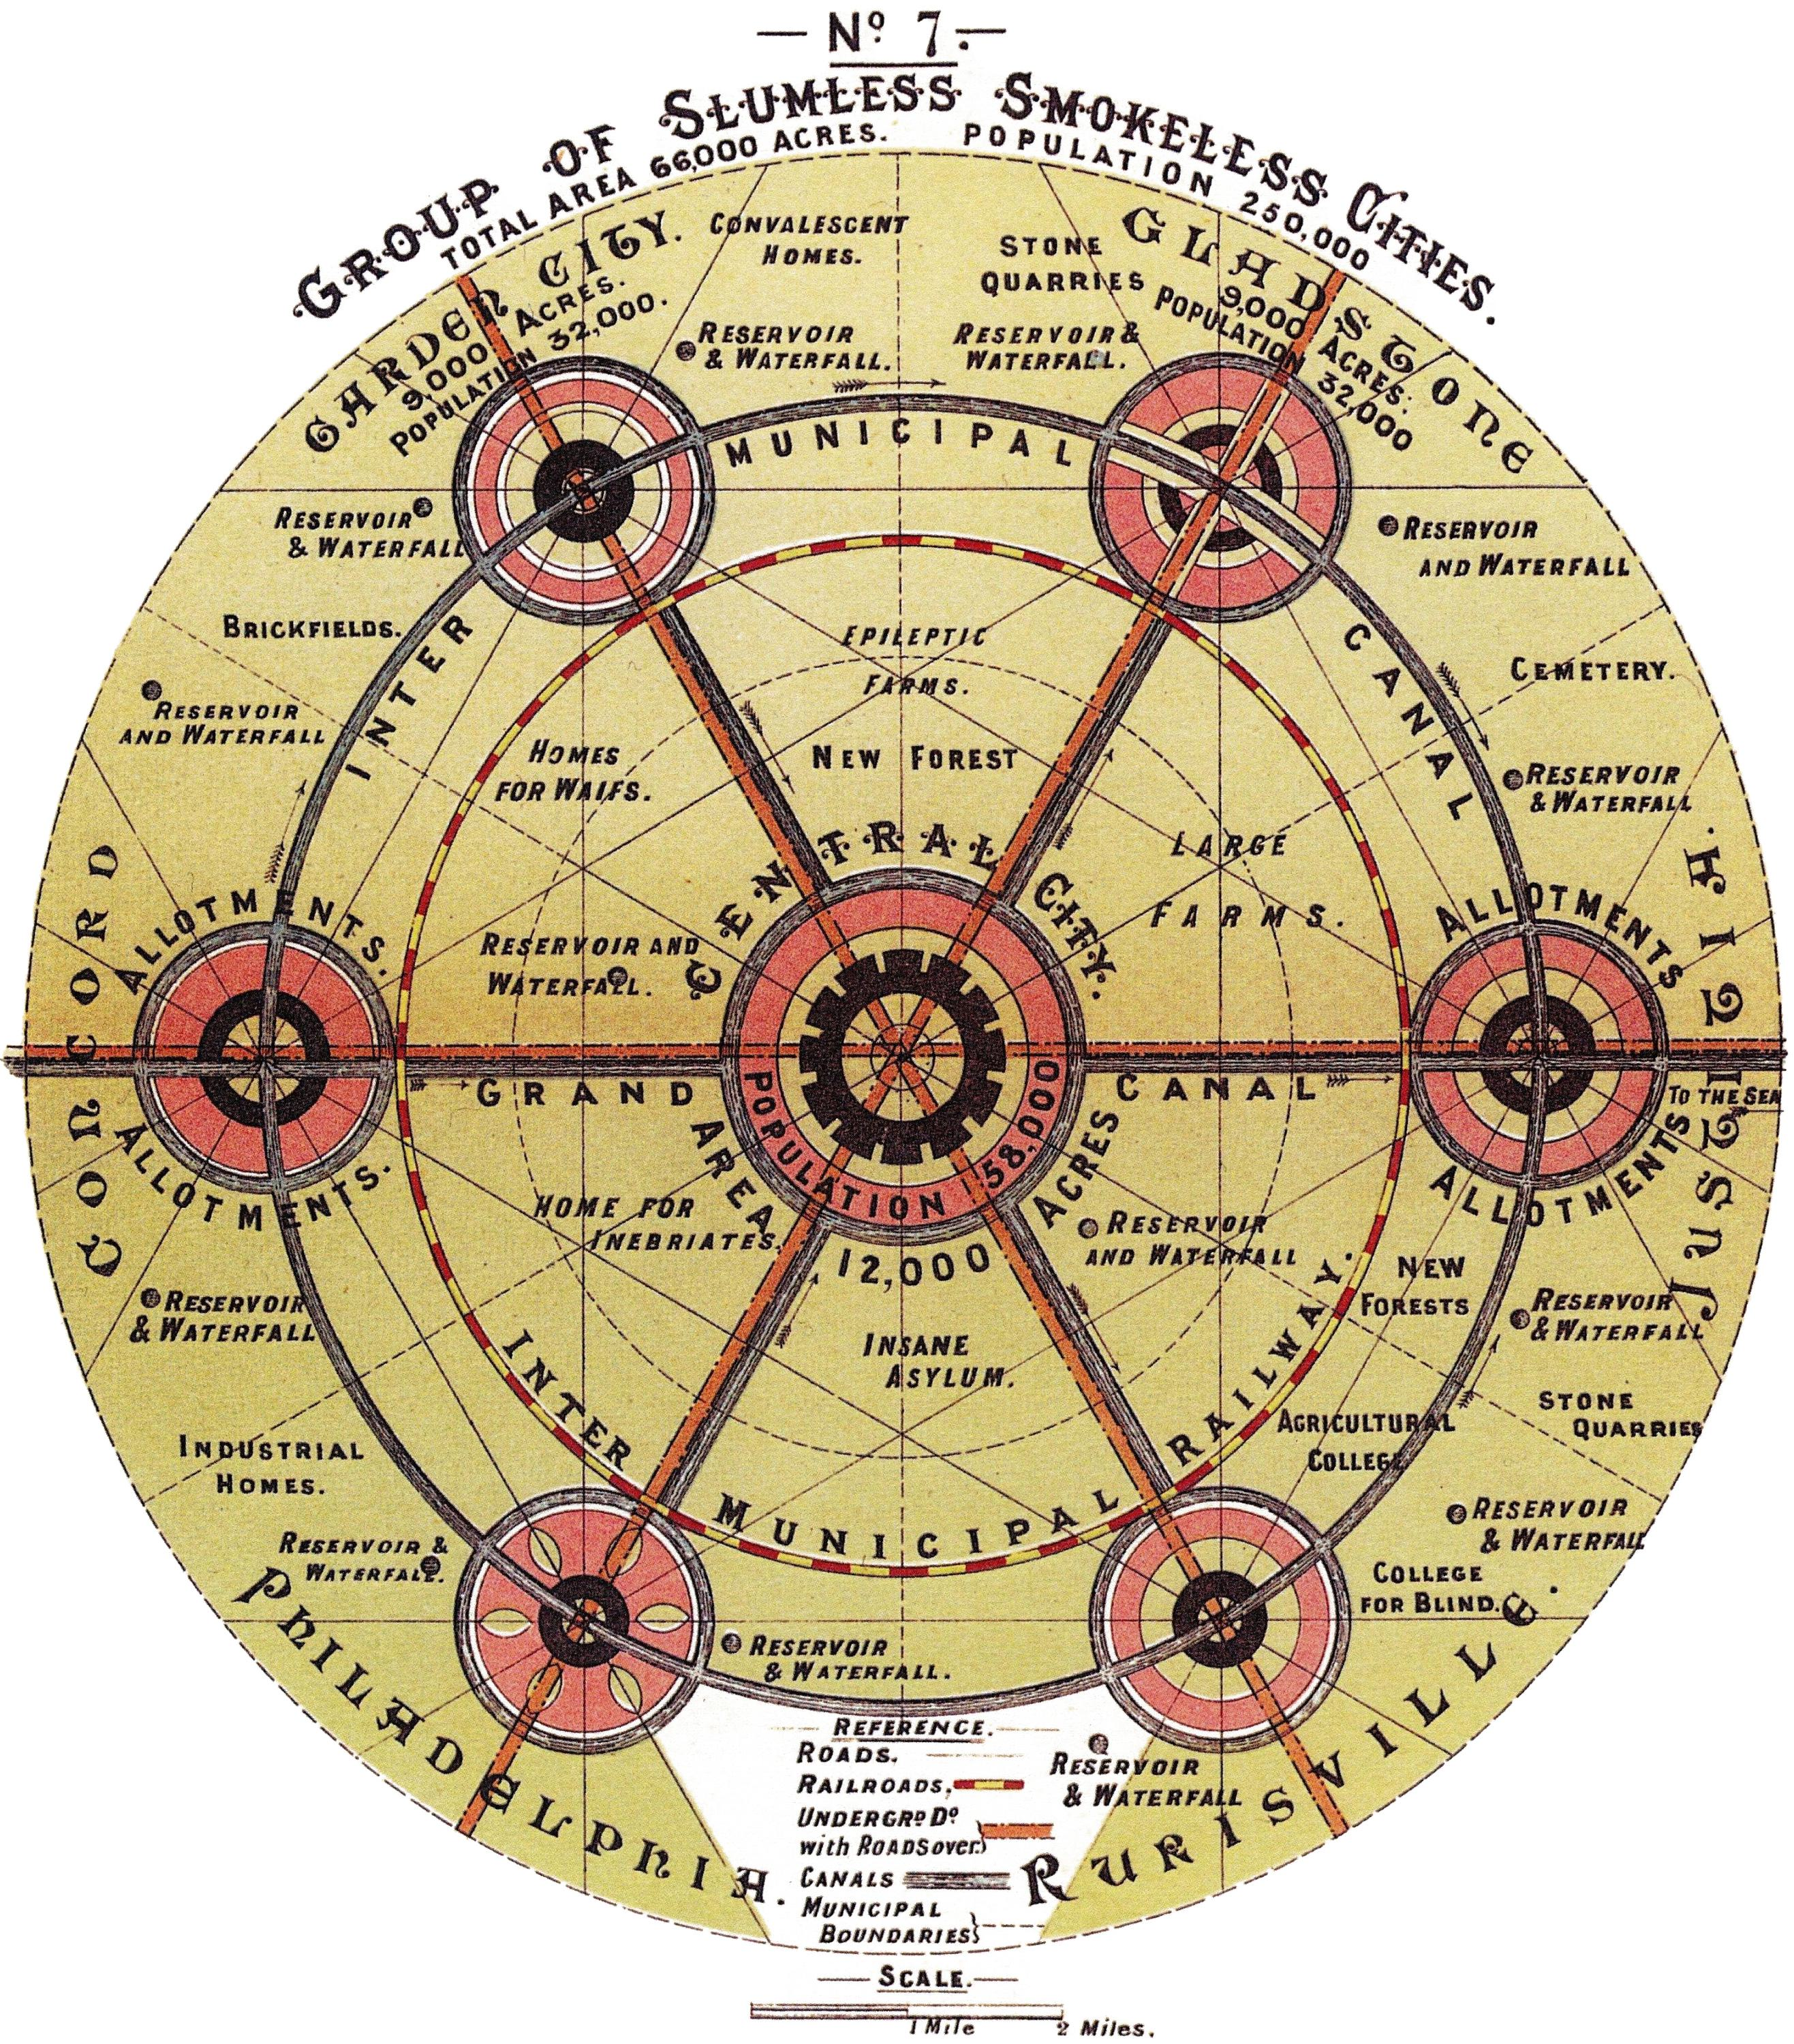
\includegraphics[width=0.75\columnwidth]{src/Figures/Chap-1/Cite_jardin.jpg}}
    \vspace{5pt}
    \begin{flushright}\scriptsize{
    Source: \textcolor{blue}{Ebenezer} \textcolor{blue}{\textcite[90]{howard_-morrow_1898}}\index{Howard, Ebenezer|pagebf}, cited by \textcolor{blue}{Stephen} \textcolor{blue}{\textcite[3]{ward_garden_1992}}\index{Ward, Stephen|pagebf}
    }\end{flushright}
\end{carte}

% Cité linéaire : théorie
Another utopian city concept that inspired \acrshort{TOD} is undoubtedly the \textsl{Linear City} (\textsl{Ciudad Lineal}), developed by \textcolor{blue}{Arturo Soria y Mata} in 1882 \textcolor{blue}{\autocite{lemelson_center_george_2014}}\index{Lemelson Center@\textsl{Lemelson Center}|pagebf}. By directing the urban expansion project over more than five kilometers along Madrid, the Spanish urban planner adopted a linear form to connect dense urban centers from the peripheries, an approach reminiscent of the corridor concept central to \acrshort{TOD} \textcolor{blue}{\autocite[348]{lopez_rodriguez_arturo_2017}}\index{López Rodríguez, Armando|pagebf}. The organization of the \textsl{Linear City} relies on a public transport mode, often the tramway, which becomes the backbone of the agglomeration \textcolor{blue}{\autocite{lemelson_center_george_2014}}\index{Lemelson Center@\textsl{Lemelson Center}|pagebf}. Unlike traditional urban growth, this urban utopia envisions a city without suburbs, capable of controlling its expansion along a corridor \textcolor{blue}{\autocite[722]{furundzic_infrastructure_2012}}\index{Furundzic, Danilo~S.|pagebf}\index{Furundzic, Bozidar~S.|pagebf}. Furthermore, the \Commas{matrix of this urban structure} is distinguished by privileged pedestrian accessibility, thanks to transverse promenades linking medium-density blocks. These two urban utopias—the \textsl{Garden City} and the \textsl{Linear City}—thus raise questions that remain relevant today and have significantly influenced \acrshort{TOD}, namely the promotion of a compact city designed both by and for public transport and walking \textcolor{blue}{\autocite[11]{salomon_cavin_cites-jardins_2007}}\index{Salomon Cavin, Joëlle|pagebf}.%%Translated%%

% Cité linéaire : exemples
The experimentation of this ideal city, initially envisioned to extend 53 kilometers around Madrid in a loop, ultimately saw only 5 kilometers realized, north-east of the Spanish capital, starting from 1894 \textcolor{blue}{\autocite[722]{furundzic_infrastructure_2012}}\index{Furundzic, Danilo~S.|pagebf}\index{Furundzic, Bozidar~S.|pagebf}. This project, designed by \textcolor{blue}{Arturo Soria y Mata}, planned radioconcentric connections linking this urban belt to the old city. In line with the hygienist city movement, this model exploited an axis encircling the existing city to facilitate the circulation of essential infrastructures such as railways, urban heating networks, electricity, or telephony. The horizontal organization of the linear city broke with the vertical structuring typical of the bourgeois city, while anticipating certain principles of the garden city, notably generalized access to individual property. More broadly, this concept evokes the notion of the \Commas{Urban Corridor} \textcolor{blue}{\autocite[63]{liu_corridors_2016}}\index{Liu, Liu|pagebf}\index{Menerault, Philippe|pagebf}\index{L'Hostis, Alain|pagebf}, allowing cities to expand linearly. In this regard, urban projects such as the \Commas{Grand Boulevard} connecting Lille, Roubaix, and Tourcoing can be seen as resonating with these principles. Inaugurated in 1909, this strategic artery, 14 kilometers long and 50 meters wide, features six circulation spaces dedicated respectively to automobiles, heavy horse-drawn transport, the Mongy tramway, riders, cyclists, and pedestrians who benefit from wide promenades\footnote{~
    Today, the Grand Boulevard is nonetheless perceived as a space more akin to an automobile transit area \textcolor{blue}{\autocite[139]{maitre_ambivalence_2016}}\index{Maitre, Elisa|pagebf}. Initially designed as an urban artery integrating two separate roadways, cycle paths, and sidewalks, this development has gradually evolved into an urban expressway, as successive connections have increased the traffic it supports. \textcolor{blue}{Philippe} \textcolor{blue}{\textcite[155]{menerault_gares_2008}}\index{Menerault, Philippe|pagebf} cites its integration with the A1 motorway, whose first section to Carvin was opened in 1954, and the A25 motorway towards Dunkirk in 1972.
} \textcolor{blue}{\autocite[87]{demangeon_lille-roubaix-tourcoing_1988}}\index{Demangeon, Alain|pagebf}\index{Werquin, Ann-Carol|pagebf}. Conceived as a structuring tool for urban growth, this project aimed to make the Grand Boulevard a regional showcase, nicknamed the \Commas{Champs-Élysées} of the metropolis, and to serve as the backbone of the future metropolis \textcolor{blue}{\autocite{dubuis__2020}}\index{Dubuis, Angélique Da Silva|pagebf}. The linear city has also inspired other interpretations and extensions, notably in Soviet experiments or through the reappropriation of this concept by \textcolor{blue}{Le Corbusier}. More recently, a notable example is the \textsl{The Line} project, announced by Saudi authorities as part of the Vision 2030 plan \textcolor{blue}{\autocite[139]{arnault_ville_2022}}\index{Arnault, Julie|pagebf}. Part of the new city project \textsl{Neom}, this concept, currently under construction, involves creating a linear city 170 kilometers long, 200 meters wide, and 500 meters high\footnote{~
    However, even before its concrete launch, the \textsl{The Line} project has been scaled back for 2030, with an infrastructure only 2.4 kilometers long instead of the initially planned 170 kilometers.
}. This infrastructure will be served by a high-speed train, theoretically allowing the entire city to be traversed in less than 20 minutes. Essential services will be distributed vertically, on each floor, and accessible in less than five minutes \textcolor{blue}{\autocite[139]{arnault_ville_2022}}\index{Arnault, Julie|pagebf}.%%Translated%%

% New Urbanism
From a more contemporary perspective, the roots of \acrshort{TOD} can be traced directly to \textsl{New Urbanism}, an urban planning and architectural movement that emerged in the 1980s in response to the limitations of modern urbanism \textcolor{blue}{\autocite[71]{liu_analyse_2016}}\index{Liu, Liu|pagebf}. This movement critiques the lack of functional and architectural diversity, the inadequate organization of public spaces, and the insufficient consideration given to pedestrians. Proposed as a rational alternative to the development of low-density, automobile-dominated suburban subdivisions, \textsl{New Urbanism} aims to rethink urban planning to make it more humane, aesthetically pleasing, and functional. Although inspired by certain principles of the modern movement, it distinguishes itself notably through the establishment, in 1989, of the \textsl{Congress for the New Urbanism}, often seen as the contemporary equivalent of the \acrfull{CIAM}. In 1996, this Congress ratified its own \textsl{Charter of the New Urbanism}\footnote{~
    This movement is not a monolithic bloc. It comprises two main complementary approaches \textcolor{blue}{\autocite[178]{ouellet_smart_2006}}\index{Ouellet, Michel|pagebf}. On one hand, the advocates of the \acrfull{TND} who emphasize a neotraditional aesthetic and urban organization, favoring compact neighborhoods with housing aligned along multi-intersection streets. On the other hand, the proponents of \acrshort{TOD} who prioritize the integration of public transport and more environmentally respectful regional urban planning. Although distinct, these two visions share a common objective: encouraging urban forms that promote functional mixity and reduce the ecological footprint of territories.
}. This \Commas{planning philosophy} advocates for compact urban development, planned on a human scale, that prioritizes public transport and the integration of diverse urban functions \textcolor{blue}{\autocite[177]{ouellet_smart_2006}}\index{Ouellet, Michel|pagebf}. From a practical standpoint, it recognizes several key characteristics of a neighborhood, including its optimal size, estimated at 400 meters from the center to the periphery \textcolor{blue}{\autocite[194]{ducharme_ville_2021}}\index{Ducharme, Olivier|pagebf}. Finally, \textsl{New Urbanism} adopts a regional perspective, considering the region as the basic territorial unit in a context of economic globalization \textcolor{blue}{\autocite[]{calthorpe_regional_2001}}\index{Calthorpe, Peter|pagebf}\index{Fulton, William|pagebf}. In this perspective, \acrshort{TOD} inherits the objective of promoting public transport to curb the artificialization of non-urbanized land \textcolor{blue}{\autocite[117]{lo_feudo_scenario_2014}}\index{Lo Feudo, Fausto|pagebf}\index{Menerault, Philippe|pagebf}\index{L'Hostis, Alain|pagebf}\index{Festa, Demetrio Carmine|pagebf}.%%Translated%%

% Smart Growth
The principles of \acrshort{TOD} also find their roots in a major contemporary urban planning movement: \textsl{Smart Growth}, which emerged in the late 1980s and became structured in the mid-1990s as an extension of the \Commas{sustainable urban development} paradigm \textcolor{blue}{\autocites[7]{bentayou_transit-oriented_2015}[71]{liu_analyse_2016}}\index{Bentayou, Gilles|pagebf}\index{Liu, Liu|pagebf}. This movement aims to preserve natural and financial resources while seeking to reduce spatial segregations, whether functional or social \textcolor{blue}{\autocite[7]{bentayou_transit-oriented_2015}}\index{Bentayou, Gilles|pagebf}. \textsl{Smart Growth} explicitly opposes uncontrolled urban sprawl by promoting more compact forms of development and urban redevelopment \textcolor{blue}{\autocites[176]{ouellet_smart_2006}{smart_growth_network_what_2015}}\index{Ouellet, Michel|pagebf}\index{Smart Growth Network@\textsl{Smart Growth Network}|pagebf}. These principles, shared by \textsl{New Urbanism}, value an integrated approach where transport and urban planning converge to create sustainable, socially equitable, and economically viable environments. \acrshort{TOD} is thus one of the tools enabling the realization of this \Commas{new} \Commas{smart} urbanism \textcolor{blue}{\autocite[7]{bentayou_transit-oriented_2015}}\index{Bentayou, Gilles|pagebf}.%%Translated%%

% Figure photographies Val d'Europe
\begin{figure}[h!]\vspace*{4pt}
    \caption{Photographs of the Val d'Europe sector, September 13, 2023.}
    \label{fig-chap1:photographies-val-europe}
    \centerline{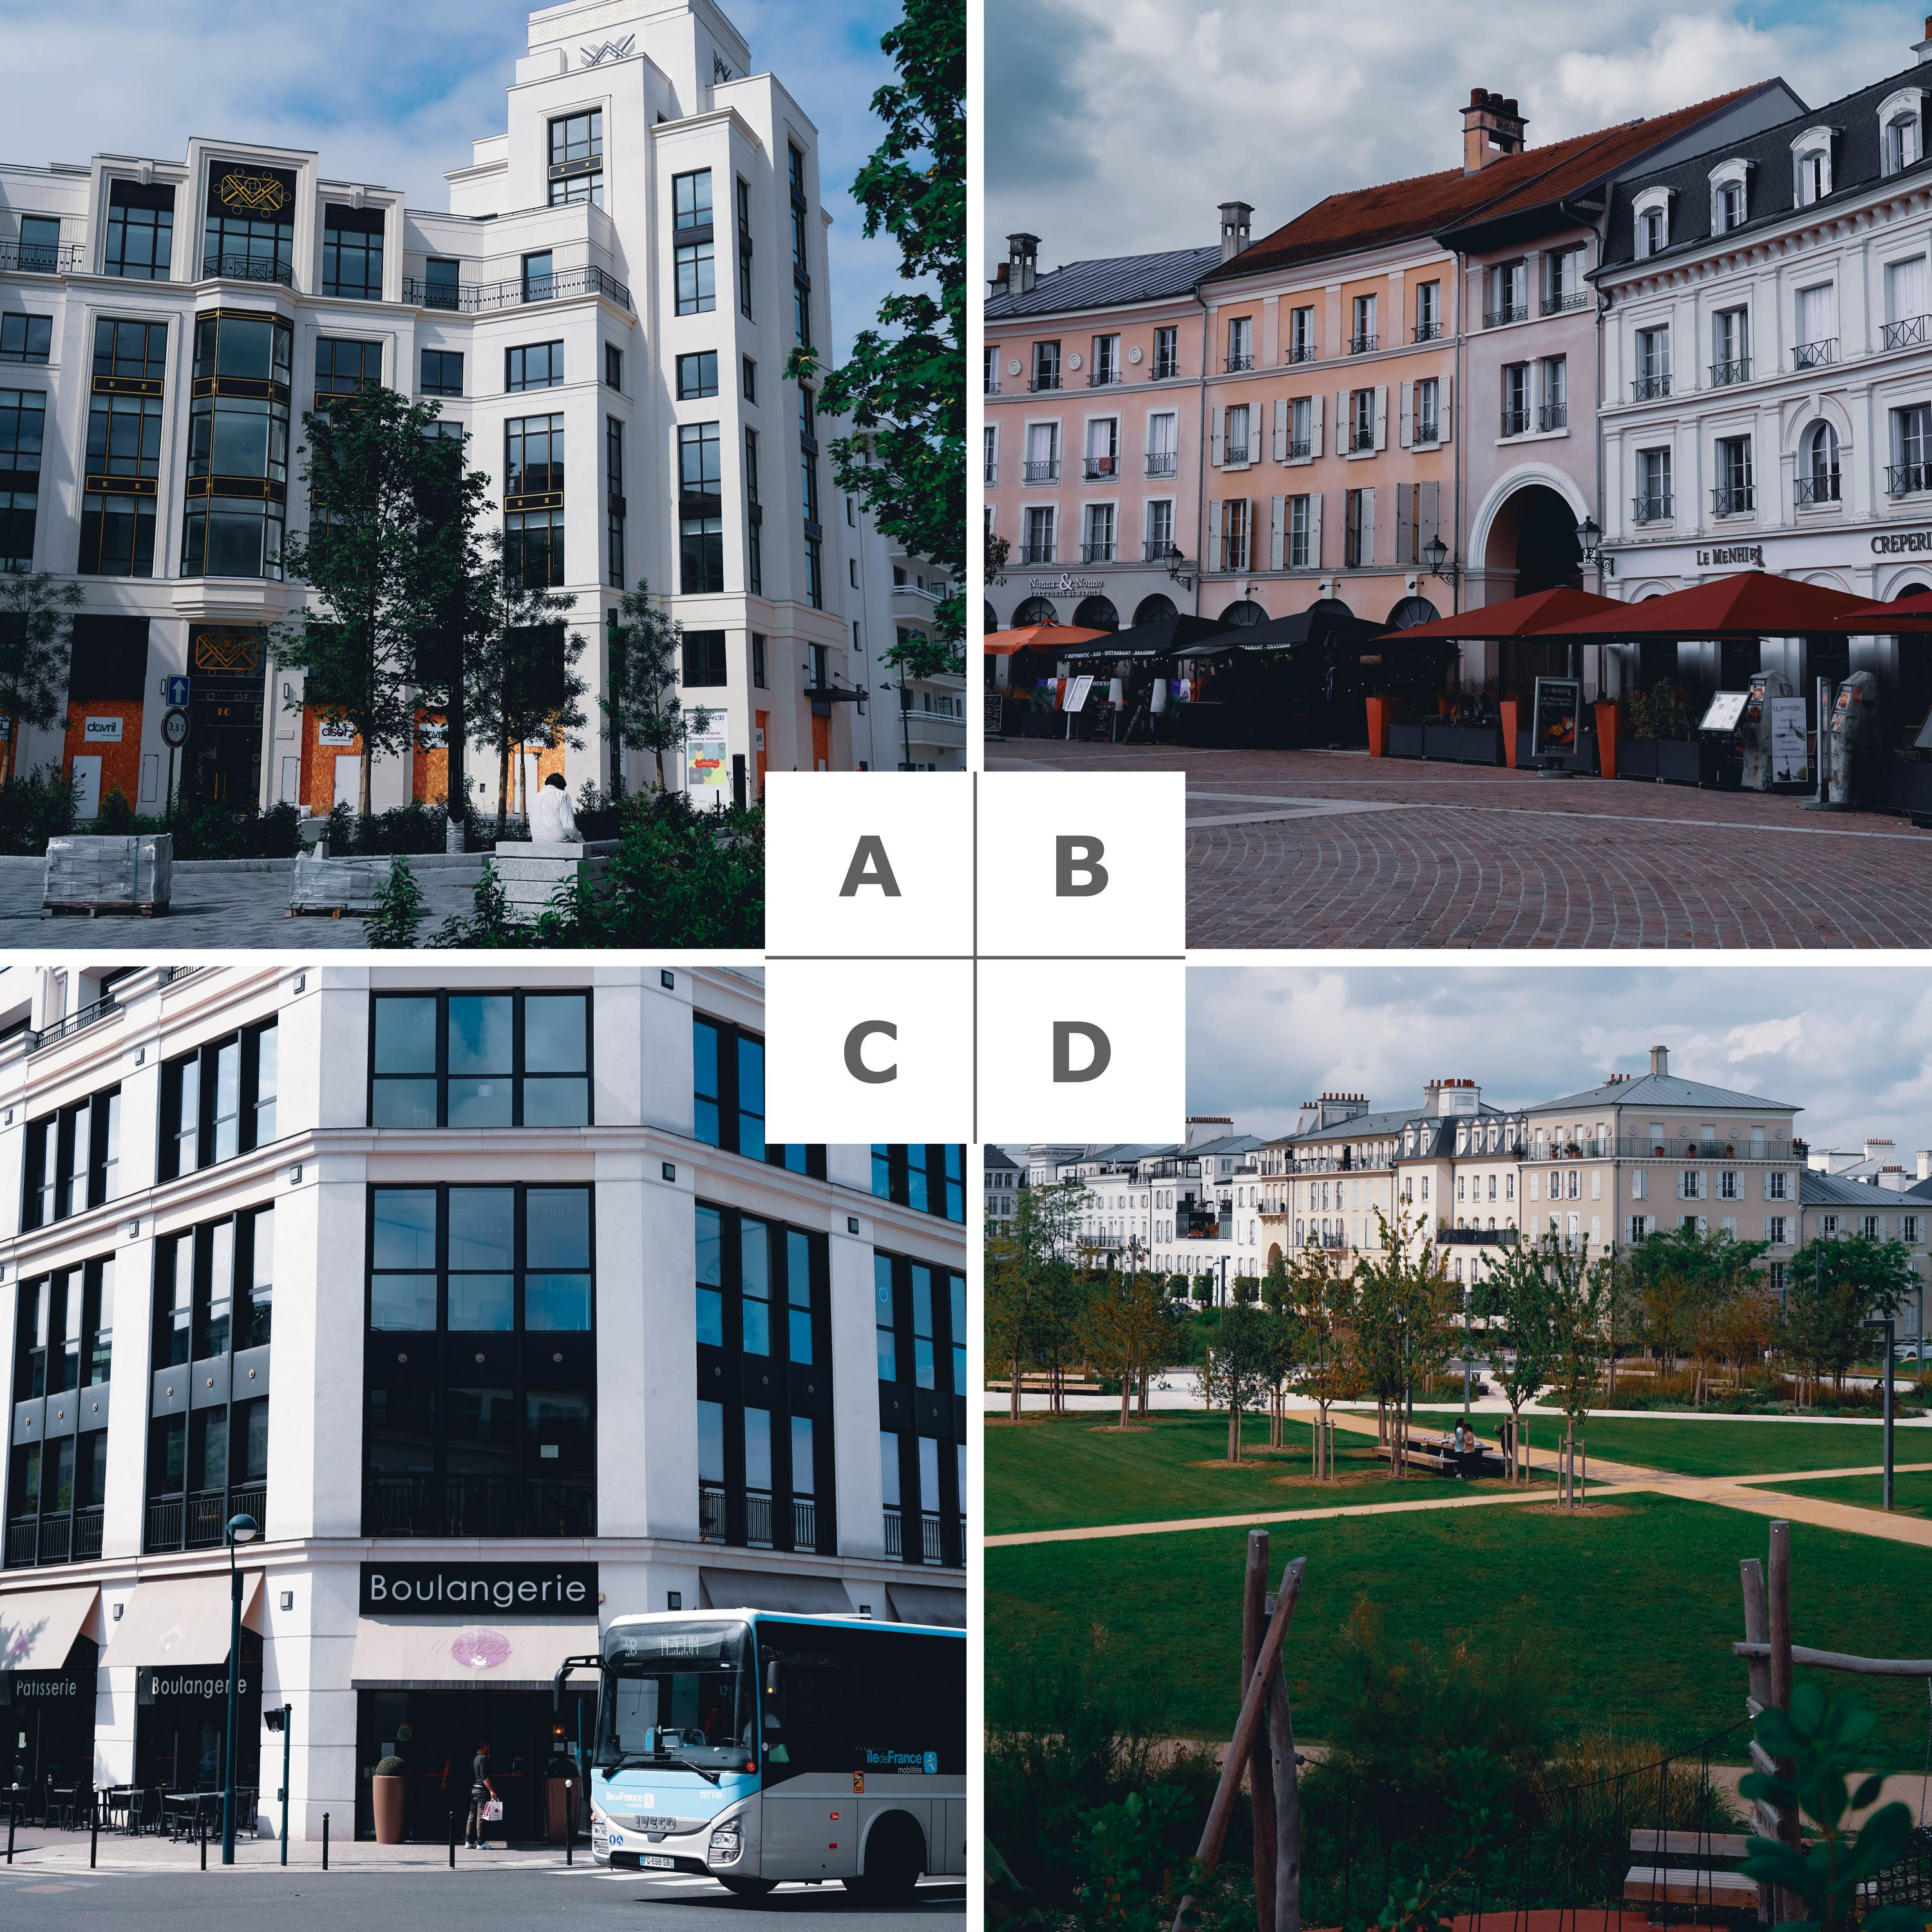
\includegraphics[width=0.75\columnwidth]{src/Figures/Chap-1/Val_Europe.jpg}}
    \vspace{5pt}
    \begin{flushright}\scriptsize{
    Photographies (A), (B), (C), and (D): \textcolor{blue}{Dylan Moinse (2023)}
  }\end{flushright}
\end{figure}

% Exemples New Urbanism/Smart Growth
Exemplary achievements illustrate the principles of \textsl{New Urbanism} and \textsl{Smart Growth}, such as the residential neighborhood of Laguna West in Sacramento, California, developed by \textcolor{blue}{Peter} \textcolor{blue}{\textcite[146-149]{calthorpe_next_1993}}\index{Calthorpe, Peter|pagebf}, a key figure in these movements. This is a \Commas{neotraditional} community, with the project launched in 1989 integrating 3,400 residential units, based on the pioneering concepts of American architect and urban planner \textcolor{blue}{Morris} \textcolor{blue}{\textcite[]{newman_focus_1991-1}}\index{Newman, Morris|pagebf}. Additionally, we examine the urban project Val d'Europe, the fourth sector of the new town of Marne-la-Vallée, awarded the \textsl{Charter Awards} in 2006 by the \textcolor{blue}{\textcite{congress_for_the_new_urbanism_cnu_2006}}\index{Congress for the New Urbanism@\textsl{Congress for the New Urbanism}|pagebf}. This urban project, developed along the A line of the \acrfull{RER} in the Paris region—the busiest line in Europe, inaugurated in 1969, although the Val d'Europe station opened in 2001—benefits from a strategic location near the Marne-la-Vallée—Chessy \acrshort{HST} station. It is a \acrfull{PPP} born from a collaboration between the French state and the \Marque{Walt Disney Company}, sealed by an agreement in 1987, aiming to develop and operate \Marque{Euro Disneyland} while integrating an urban center into the new town \textcolor{blue}{\autocite{epamarne_val_nodate}}\footnote{~
    The \acrfull{EPA} ÉpaMarne, in collaboration with ÉpaFrance, was tasked with overseeing Val d'Europe as part of a strategy to balance the territorial development of the Île-de-France region, traditionally dominated by the attractiveness of the \acrfull{CBD} of La Défense. This project embodies a dual ambition: creating an autonomous urban center on the outskirts of Paris and enhancing regional tourism appeal through the establishment of Disneyland Paris.
}. The planning of Val d'Europe is based on three principles aligned with the aforementioned movements: (i) an organization into neighborhoods, squares, and streets, favoring human scales; (ii) social and functional diversity, integrating housing\footnote{~
    The urban development of Val d'Europe continues. Adopted in 2016, the first \acrfull{PLUi} of the \acrshort{EPCI} plans the construction of 650 housing units per year, aiming for a total of 5,100 units, with 80\% being family homes. This plan also aims to meet the requirements of the \acrfull{SRU} regarding social housing, with 34\% of future housing being social housing, according to its \acrfull{PLH}.
}, commerce, and services\footnote{~
    For example, the Val d'Europe shopping center, opened in 2000, serves as the symbolic and functional heart of the city. It is divided into thematic zones and has been awarded for its design (\textsl{International Council of Shopping Centers Europe awards}).
}; and (iii) architecture inspired by European history, conferring an identity to each neighborhood (see \hyperref[fig-chap1:photographies-val-europe]{Figure~\ref{fig-chap1:photographies-val-europe}}, page~\pageref{fig-chap1:photographies-val-europe}). As \textcolor{blue}{\textcite[25]{dupuis_nouvelle_2017}}\index{Dupuis, Blaise|pagebf}\index{Söderström, Ola|pagebf} explain, Val d'Europe, as a \Commas{new traditional town}, embodies the principles advocated\footnote{~
    However, the development of Val d'Europe raises questions about its governance model and urban design. The involvement of a private operator in urban management has imposed a commercial vision of urban development. This approach has often been criticized for its tendency towards \Commas{Disneyfication} or \Commas{museification} of urban space \textcolor{blue}{\autocite[]{brunel_planete_2012}}\index{Brunel, Sylvie|pagebf}. These notions refer to an idealized and hyper-controlled model, characterized by a fictional and standardized reproduction of urban landscapes and histories, designed to meet the stereotypical expectations of tourists \textcolor{blue}{\autocite[7]{claude_developpement_2021}}\index{Claude, Appolline|pagebf}\index{Laage de Meux, Olivia de|pagebf}\index{Delpuech, Inès|pagebf}\index{Dextreit, Natalia|pagebf}\index{Poquillon, Mathilde|pagebf}\index{Praderie, Mila|pagebf}. Critics also highlight the risks of disconnection between this idealized city and social and economic realities. They question the balance between entrepreneurial imperatives, social inclusion, and sustainability. Furthermore, the negotiation processes between public and private actors have been marked by tensions, revealing the limits of a \acrshort{PPP} in such urban projects. An example is the location of the regional shopping center Val d'Europe. The private operator, likely influenced by a \Commas{culture of indifference towards public transport} \textcolor{blue}{\autocite[656]{tan_identifying_2014}}\index{Tan, Wendy|pagebf}\index{Bertolini, Luca|pagebf}\index{Janssen-Jansen, Leonie|pagebf}, wanted to locate this facility on the outskirts of the highway, far from the transit hub and the \acrshort{RER} station.
}, namely urban compactness, neighborhood organization, and aesthetic and morphological principles rooted in the heritage of past centuries \textcolor{blue}{\autocite[12]{moinse_exploring_2023}}\index{Moinse, Dylan|pagebf}.%%Translated%%

% Transition
The concept of \acrshort{TOD}, centered on compact, mixed, and transit-oriented urban development, draws from a lineage of urban planning movements that preceded it. These influences are fully acknowledged by \textcolor{blue}{Peter Calthorpe}, one of the main theorists of \acrshort{TOD}, who defines himself as a \Commas{restorer rather than an originator of ideas}\footnote{~
    \Commas{\textsl{Mr. Calthorpe, who calls himself a reviver rather than an originator of ideas} [\dots]} \textcolor{blue}{\autocite[5]{newman_focus_1991}}\index{Newman, Morris|pagebf}.
} \textcolor{blue}{\autocite[5]{newman_focus_1991}}\index{Newman, Morris|pagebf}. While the precursors of \acrshort{TOD} can be identified in models such as the \textsl{Garden City} or the \textsl{Linear City}, or in major figures of urban planning history like \textcolor{blue}{Ildefons Cerdà} or \textcolor{blue}{Georges-Eugène Haussmann}, these examples illustrate the evolution of ideas in urban planning. In the garden city, for instance, the train station plays a limited functional role, merely connecting self-sufficient cities to each other and their environment. \textcolor{blue}{Peter} \textcolor{blue}{\textcite[43-49]{calthorpe_next_1993}}\index{Calthorpe, Peter|pagebf}, on the other hand, reverses this principle: in \acrshort{TOD}, the transit station becomes the structuring center of urban development, moving beyond the logic of self-sufficiency to create connections within a fragmented and dispersed contemporary city \textcolor{blue}{\autocite[51]{el_hadeuf_ville_2017}}\index{El Hadeuf, Mounya|pagebf}\index{Laterrasse, Jean|pagebf}. This distinction marks a conceptual turning point. Unlike \textsl{New Urbanism} and \textsl{Smart Growth}, which primarily oppose uncontrolled urban sprawl, \acrshort{TOD} asserts a leading role for transport infrastructure in structuring the city \textcolor{blue}{\autocite[51]{el_hadeuf_ville_2017}}\index{El Hadeuf, Mounya|pagebf}\index{Laterrasse, Jean|pagebf}. Where \textsl{New Urbanism} promotes human-scale density and aesthetics, and \textsl{Smart Growth} prioritizes the preservation of natural resources and functional diversity, \acrshort{TOD} distinguishes itself by its ambition to reconnect dispersed territories through a transport-centered organization. Although most morphological components—such as the presence of a station, density, and compactness—are similar, this approach reflects a shift in scale between the 19\textsuperscript{th}-century city, still conceived as a coherent whole, and the contemporary city, which requires tools to restore its cohesion \textcolor{blue}{\autocite[37]{leysens_reconfiguration_2011}}\index{Leysens, Thomas|pagebf}\index{Menerault, Philippe|pagebf}\index{L'Hostis, Alain|pagebf}.%%Translated%%

% 1.1.1.2. TOD aspects contemporains
\needspace{1\baselineskip} % Reserve space
\subsubsection*{Originality and Reinterpretation of Planning Around Rail
    \label{chap1:tod-presentation-generale-origines-originalite}
    }

% Introduction
The movement that gave rise to \acrshort{TOD} is part of an intellectual and urban planning lineage shared by several critical and activist currents, united in their opposition to the car-centric city paradigm\footnote{~
    Since the 1960s, and even post-war, the dominance of the automobile in urban spaces began to be questioned, sparking growing criticism of its mass use and implications for urban planning \textcolor{blue}{\autocites{jacobs_death_1961}{illich_energie_1973}}\index{Jacobs, Jane|pagebf}\index{Illich, Ivan|pagebf}\index{Giard, Luce|pagebf}\index{Bardet, Vincent|pagebf}. This transition to the \Commas{third age of the city} \textcolor{blue}{\autocite[4]{newman_land_1996}}\index{Newman, Peter W.~G.|pagebf}\index{Kenworthy, Jeffrey~R.|pagebf}, marked by the \Commas{culture of the automobile} \textcolor{blue}{\autocite[157]{urry_social_2003}}\index{Urry, John|pagebf}, still structures most territories today, with direct and indirect consequences for planning, mobility behaviors, and lifestyles \textcolor{blue}{\autocite[40]{sebban_complementarite_2003}}\index{Sebban, Annie-Claude|pagebf}\index{Motte, Alain|pagebf}.
}. \textcolor{blue}{\autocites{jacobs_death_1961}{illich_energie_1973}}\index{Jacobs, Jane|pagebf}\index{Illich, Ivan|pagebf}\index{Giard, Luce|pagebf}\index{Bardet, Vincent|pagebf}, and particularly the numerous negative externalities associated with this model\footnote{~
    The negative externalities generated by automobile dependence include internal nuisances such as urban congestion, which compromises the economic and residential attractiveness of territories, as well as broader external effects: road accidents, urban fragmentation, socio-spatial exclusion, increased consumption of agricultural and natural spaces, loss of biodiversity, multiple pollutions (air, water, soil, noise, and visual), and degradation of quality of life, ranging from physical and mental health issues to chronic stress and reduced productivity. These externalities contribute to what some authors refer to as the \Commas{spiral of automobile dependence} or \Commas{cycle of auto-dependence}, where the automobile creates problems that only its intensified use seems able to solve \textcolor{blue}{\autocites[62]{cervero_transit_1998}[4]{heran_reduction_2001}[2]{heran_zones_2009}}\index{Cervero, Robert|pagebf}\index{Héran, Frédéric|pagebf}\index{Pouillaude, Laurence|pagebf}.
}. \textcolor{blue}{\autocites[62]{cervero_transit_1998}[4]{heran_reduction_2001}[2]{heran_zones_2009}}\index{Cervero, Robert|pagebf}\index{Héran, Frédéric|pagebf}\index{Pouillaude, Laurence|pagebf}. The \Commas{automobile system}, characterized by an organizational mode centered on technical performance and apparent advantages of the car, constitutes a captive and rigid structure\footnote{~
    Automobile dependence, along with \Commas{automobility}—denoting a way of life and associated representations—is based on cultural, socio-economic, urban planning, and technocratic factors \textcolor{blue}{\autocite[12]{heran_reduction_2001}}\index{Héran, Frédéric|pagebf}. The \Commas{all-automobile} is the product of aspirations linked to individual home and garden ownership, elevated living standards combined with consumption norms, urban forms favoring motorized travel, and the continuous improvement of car performance relative to other modes of transport.
}. The \Commas{hidden costs} associated with this system, i.e., the costs not covered by the community, are estimated at approximately 3\% of the annual \acrfull{GDP} of the \acrfull{EU}, revealing its collective inefficiency \textcolor{blue}{\autocite[34]{becker_couts_2012}}\index{Becker, Udo~J.|pagebf}\index{Becker, Thilo|pagebf}\index{Gerlach, Julia|pagebf} and its contribution to a genuine \Commas{tragedy of the commons} \textcolor{blue}{\autocite{hardin_tragecommuns_1968}}\index{Hardin, Garrett|pagebf}, where intensive use of road spaces by certain individuals leads to detrimental consequences for society as a whole \textcolor{blue}{\autocite[23]{6t-bureau_de_recherche_livre_2019}}\index{Bureau de recherche 6t@\textsl{Bureau de recherche 6t}|pagebf}. It should be noted that these estimates remain underestimated, particularly due to the lack of systematic consideration of complex feedback loops affecting climate change and public health \textcolor{blue}{\autocite[66, 72]{gossling_social_2019}}\index{Gössling, Stephan|pagebf}\index{Choi, Andy|pagebf}\index{Dekker, Kaely|pagebf}\index{Metzler, Daniel|pagebf}. It is precisely in this critical context that the \acrshort{TOD} concept is deployed as a multidimensional response aimed at addressing the dysfunctions of the car-centric model.%%Translated%%

% Lutte contre la dépendance automobile
Indeed, more than an invention \textsl{ex nihilo}, \acrshort{TOD} primarily constitutes an adaptation to a renewed urban context, characterized by the complexity and \Commas{speed} of modern cities. It offers an articulated alternative to the widespread diffusion and use of the automobile by introducing principles, perspectives, and operational tools to address current challenges at various spatial scales \textcolor{blue}{\autocite[37]{leysens_reconfiguration_2011}}\index{Leysens, Thomas|pagebf}. This is where the original contributions of the model lie \textcolor{blue}{\autocite[121]{lo_feudo_scenario_2014}}\index{Lo Feudo, Fausto|pagebf}\index{Menerault, Philippe|pagebf}\index{L'Hostis, Alain|pagebf}\index{Festa, Demetrio Carmine|pagebf}: the idea that the automobile should no longer be the benchmark for urban space planning must be abandoned \textcolor{blue}{\autocite[190]{ducharme_ville_2021}}\index{Ducharme, Olivier|pagebf}. \textcolor{blue}{Peter} \textcolor{blue}{\textcite{calthorpe_next_1993}}\index{Calthorpe, Peter|pagebf} thus essentially formalized the close relationship between urban development and public transport, establishing it as a structuring principle of \acrshort{TOD}. In this framework, \acrshort{TOD} defines the bases of a \Commas{new American dream}: unlike preceding currents primarily focused on aesthetic or social concerns, \acrshort{TOD} favors a resolutely regional approach. It is no longer merely a collection of dispersed urban projects within a contemporary city \textcolor{blue}{\autocite[357]{mongin_ville_2013}}\index{Mongin, Olivier|pagebf}. It integrates the imperative of reducing automobile use at the very core of urban planning functions \textcolor{blue}{\autocite[11]{calthorpe_next_1993}}\index{Calthorpe, Peter|pagebf}.%%Translated%%

% Oriented
The second innovation brought by \acrshort{TOD} lies in its ability to adjust to the context of growing automobile use while proposing a collective reflection nourished by international experiences. It notably introduces a third structuring element in the relationship between \textsl{transit} and \textsl{development}: the idea of orientation (\textsl{oriented}). In this regard, this form of connection is decisive, as noted by \textcolor{blue}{Fausto} \textcolor{blue}{\textcite[116]{lo_feudo_scenario_2014}}\index{Lo Feudo, Fausto|pagebf}. This notion goes beyond mere geographical proximity to embrace a global and coherent organization of intervention zones. Consequently, the scientific community that contributed to the evolution of the \acrshort{TOD} model advocates a holistic vision of urbanism \textsl{oriented} towards public transport, making public spaces a pivot in the articulation between the network and urban development. Thus, \acrshort{TOD} is not limited to a series of isolated operations near a station \textcolor{blue}{\autocite[124]{lhostis_ville_2013}}\index{L'Hostis, Alain|pagebf}\index{Soulas, Claude|pagebf}\index{Wulfhorst, Gebhard|pagebf}\index{Brun, Gérard|pagebf}. It is part of a broader strategic logic of redistribution along the corridors of the public transport network, considering the regional spatial structure and valorizing a \Commas{trace-based, connecting, and mixed urbanism}, in contrast to the \Commas{sector-based, secure, and homogeneous urbanism} that prevails \textcolor{blue}{\autocite[4-6]{mangin_ville_2004}}\index{Mangin, David|pagebf}.%%Translated%%

% Figure Murdoch
\begin{figure}[h!]\vspace*{4pt}
    \caption{Aerial view (A) and first-person view (B) of the surroundings of Murdoch station, connected to the Transperth network, in Australia.}
    \label{fig-chap1:tad-murdoch}
    \centerline{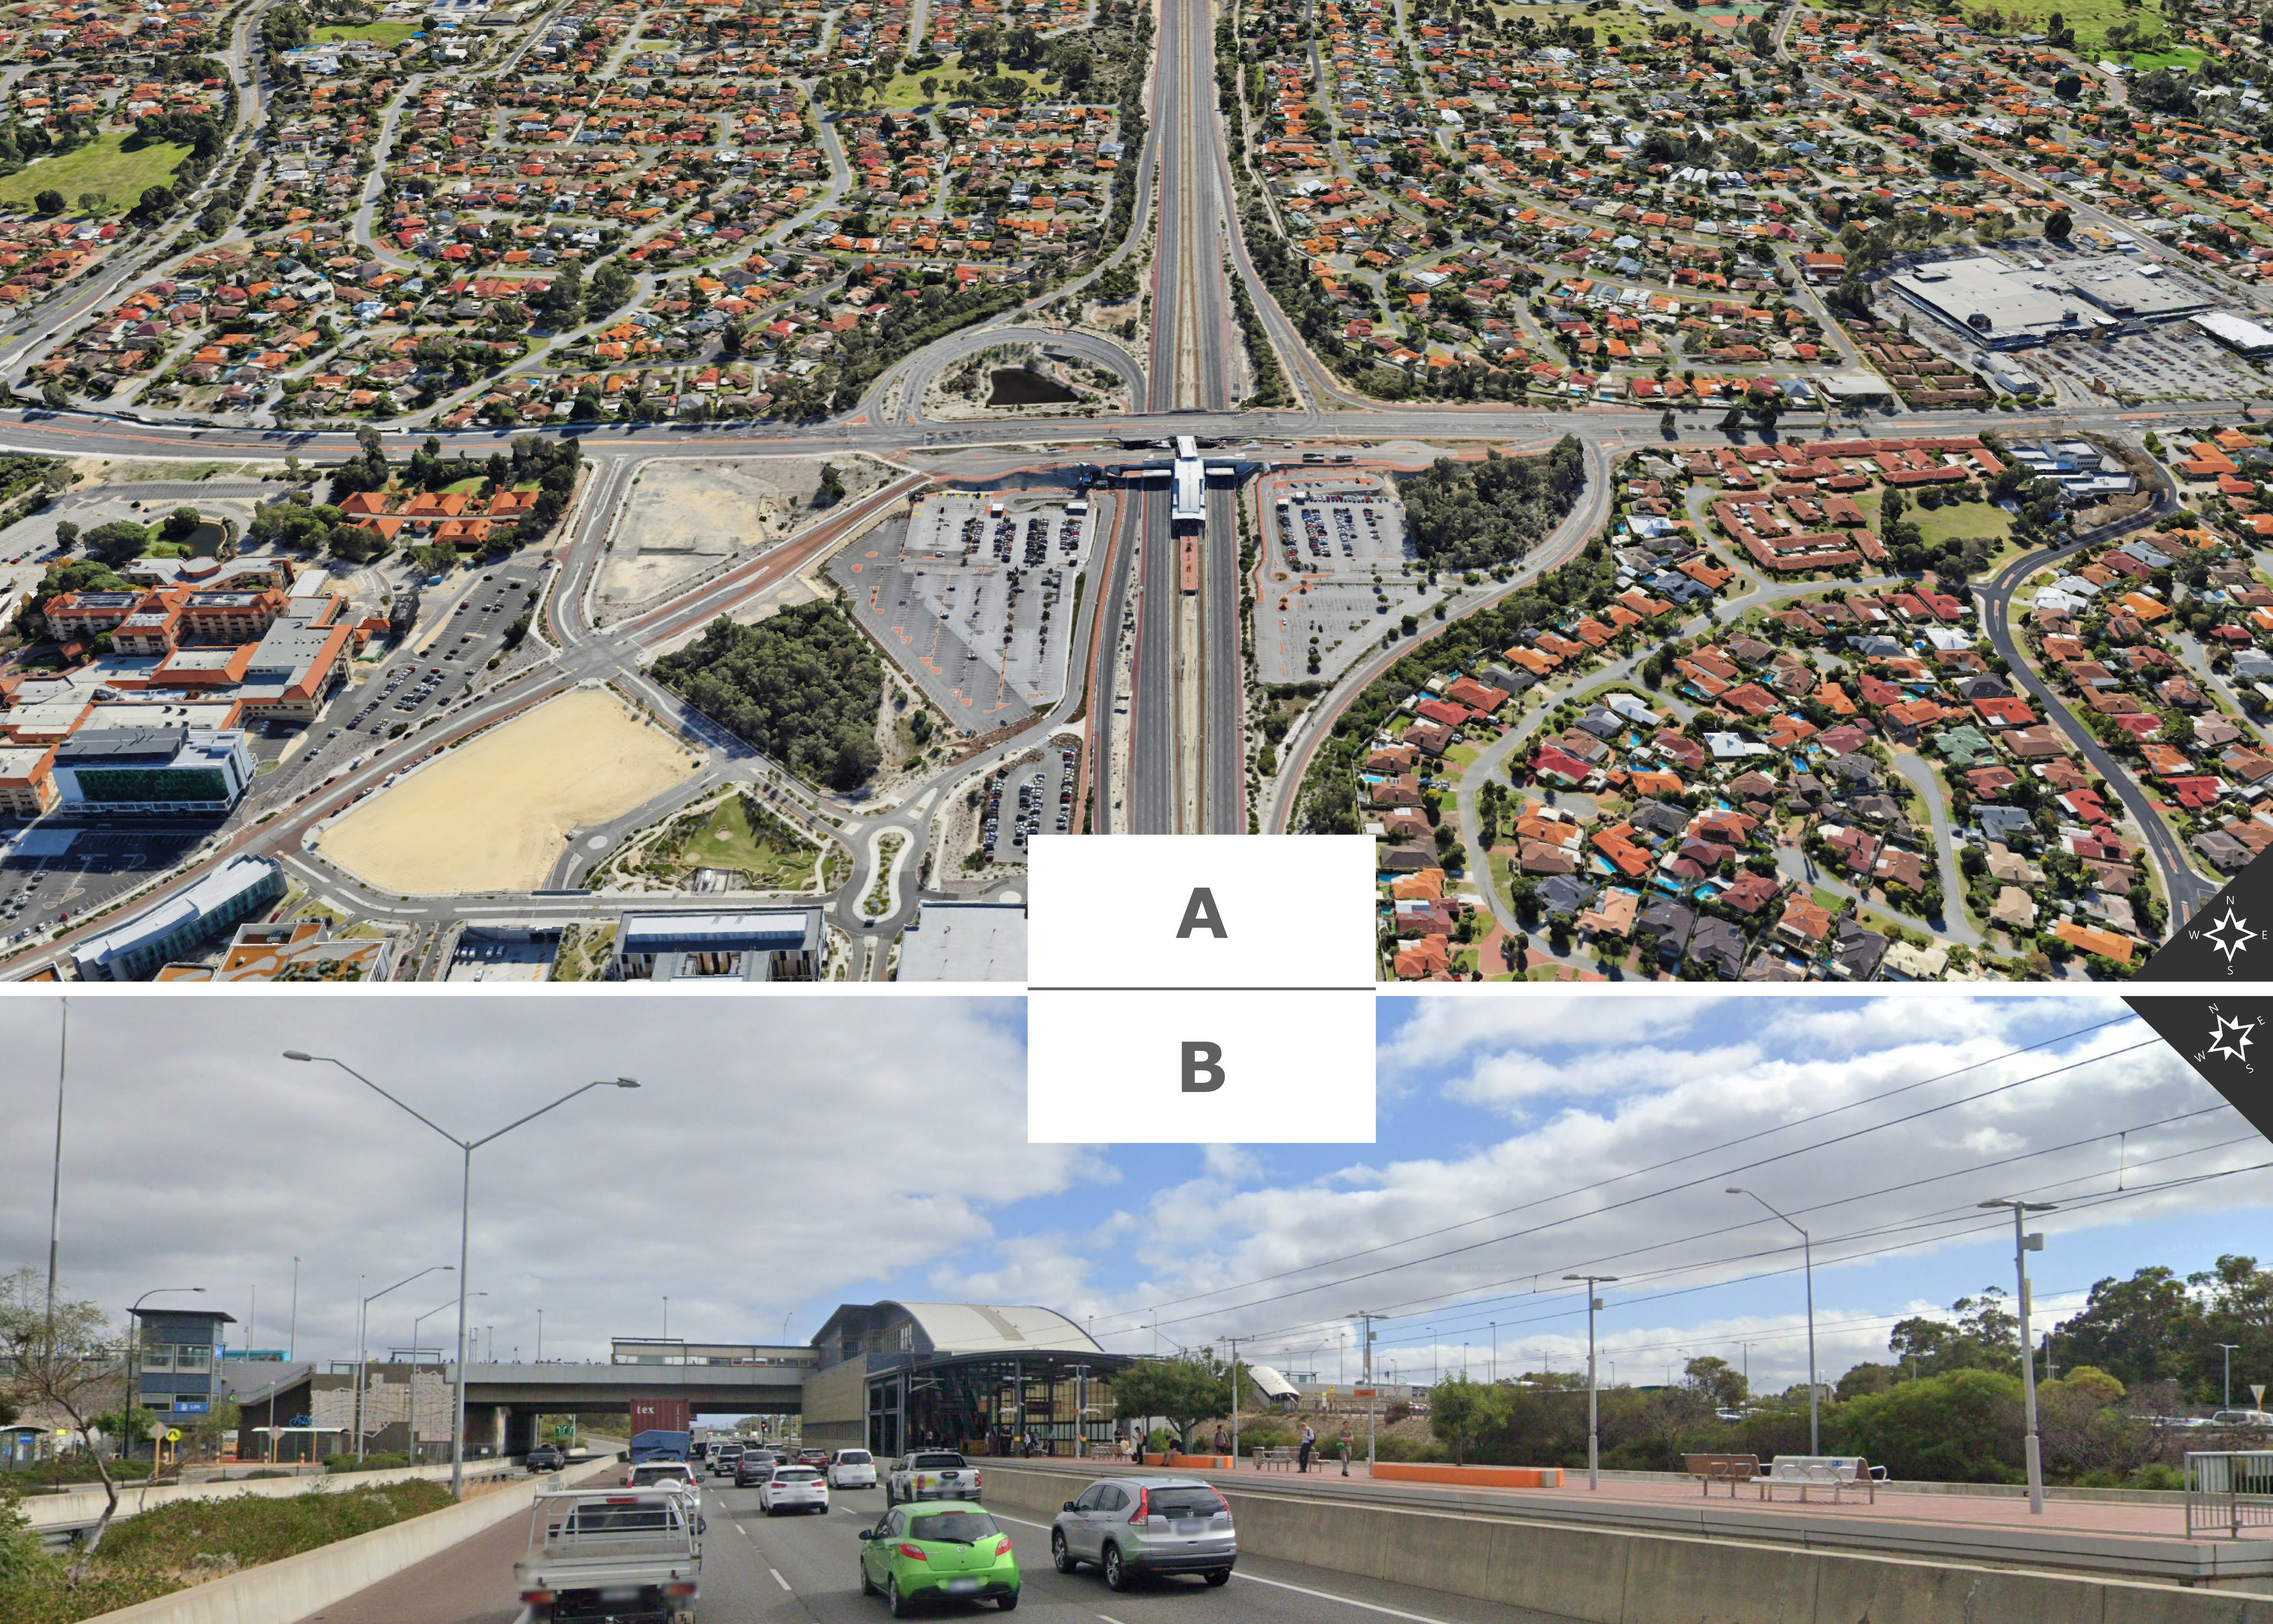
\includegraphics[width=1\columnwidth]{src/Figures/Chap-1/Murdoch.jpg}}
    \vspace{5pt}
    \begin{flushright}\scriptsize{
    Data set (A): Satellite data from \textcolor{blue}{\textcite{google_earth_google_2023}}
    \\
    Data set (B): Images from \Marque{Google Street View} dated November 2023
    }\end{flushright}
\end{figure}

% Adjacent
Consequently, a progressive distinction is made between \acrshort{TOD}\textcolor{blue}{s} that genuinely adhere to the model's principles and those that, due to interpretative or applicative divergences, do not meet the expected criteria. This diversity of approaches has led to the widespread attribution of the \acrshort{TOD} label to a broad range of urban projects that do not necessarily possess all the characteristics of the concept \textcolor{blue}{\autocite[4]{renne_transit-oriented_2013}}\index{Renne, John Luciano|pagebf}\index{Ewing, Reid|pagebf}. Among the reasons for these discrepancies are insufficient pedestrian and cycling amenities, a lack of functional diversity, and excessive automobile parking provision\footnote{~
    Several studies demonstrate that, for a majority of local U.S. authorities, automobile parking remains perceived as a more pertinent mobility and planning solution than densification around transit stations \textcolor{blue}{\autocite[106-107]{cervero_tcrp_2004}}\index{Cervero, Robert|pagebf}\index{Murphy, Steven|pagebf}\index{Ferrell, Christopher|pagebf}\index{Tsai, Yu-Hsin|pagebf}\index{Arrington,~G.~B.|pagebf}\index{Boroski, John|pagebf}\index{Smith-Heimer, Janet|pagebf}\index{Golem, Ron|pagebf}\index{Peninger, Paul|pagebf}\index{Nakajima, Eric|pagebf}\index{Chui, Ener|pagebf}\index{Dunphy, Robert|pagebf}\index{Myers, Mel|pagebf}\index{McKay, Shannon|pagebf}\index{Witenstein, Nicole|pagebf}. Many projects claiming to be \acrshort{TOD}\textcolor{blue}{s} continue to allocate significant space to surface and structured automobile parking, often to maintain existing automobile-centric logics. This persistence of the automobile as the dominant mode results from a lack of framing and reflection on its role in the planning of spaces around stations. Consequently, these \Commas{\textsl{Transit-Oriented Developments} gone wrong} have sometimes allowed the car to remain largely privileged locally \textcolor{blue}{\autocite[39]{bentayou_transit-oriented_2015}}\index{Bentayou, Gilles|pagebf}. Since then, new positions have emerged that place much greater emphasis on the determining role of automobile parking policies in the success of \acrshort{TOD} \textcolor{blue}{\autocite[39]{bentayou_transit-oriented_2015}}\index{Bentayou, Gilles|pagebf}. In particular, by advocating for strengthening regulatory requirements concerning minimum and maximum parking standards, as a reduction in parking ratios for residential projects in \acrshort{TOD}\textcolor{blue}{s} can increase potential density by 20\% to 33\% and reduce parking-related costs by 5\% to 36\%, while promoting affordable prices and improving profitability \textcolor{blue}{\autocite[51-54]{arrington_effects_2008}}\index{Arrington,~G.~B.|pagebf}\index{Cervero, Robert|pagebf}.
}. \textcolor{blue}{\autocites[358]{lund_reasons_2006}[3]{renne_transit-adjacent_2009}}\index{Lund, Hollie~M.|pagebf}\index{Renne, John Luciano|pagebf}. These shortcomings or failures often lead to these projects being more akin to \acrfull{TAD}, i.e., developments that suffer from a lack of connectivity with the public transport network. Furthermore, some projects, designated under the acronym \acrfull{TRD}, exploit proximity to a public transport network for real estate operations without integrating the fundamental principles of \acrshort{TOD} \textcolor{blue}{\autocite[18]{bentayou_transit-oriented_2015}}\index{Bentayou, Gilles|pagebf}. For example, \textcolor{blue}{\textcite[18]{khan_parking_2009}}\index{Khan, Shadhed|pagebf}\index{Bajracharya, Bhishna|pagebf} analyze the Murdoch station, located on the Mandurah line connecting Perth, Australia. The authors identify this site as a typical case of \textsl{Transit-Adjacent Development}, noting that the station's surroundings are largely dominated by highway infrastructure, road interchanges, \acrfull{PnR} facilities, and a sparse suburban fabric. \hyperref[fig-chap1:tad-murdoch]{Figure~\ref{fig-chap1:tad-murdoch}} (page~\pageref{fig-chap1:tad-murdoch}) visually depicts this spatial configuration. These \Commas{\textsl{Transit-Oriented Developments} gone wrong} thus serve as a reminder that proximity to a public transport system and urban density are not sufficient to guarantee the model's success \textcolor{blue}{\autocite[18]{bentayou_transit-oriented_2015}}\index{Bentayou, Gilles|pagebf}.%%Translated%%

% Inspirations
As we have seen, \acrshort{TOD} draws from the struggles and principles of the urban planning movements that preceded it, while readjusting them to meet the challenges of the 21\textsuperscript{st} century. \textcolor{blue}{Peter Calthorpe}, in conceptualizing \acrshort{TOD}, offered urban planning a theoretical framework and a strategic tool with international relevance, whose pertinence is supported by contributions from numerous thinkers in the fields of urbanism and transport \textcolor{blue}{\autocite[111]{almeida_correia_transit-oriented_2020}}\index{Almeida Correia, Gonçalo Homem de|pagebf}\index{Ibraeva, Anna|pagebf}\index{Silva, Cecília|pagebf}\index{Pais Antunes, António|pagebf}. In return, the \acrshort{TOD} model has inspired new approaches in urban development. \textcolor{blue}{Fausto} \textcolor{blue}{\textcite[122]{lo_feudo_scenario_2014}}\index{Lo Feudo, Fausto|pagebf}\index{Menerault, Philippe|pagebf}\index{L'Hostis, Alain|pagebf}\index{Festa, Demetrio Carmine|pagebf} highlights three recent lines of reflection that extend the urban model's legacy by reimagining proximity through a coordinated approach between urbanism and mobility:
\begin{customitemize}
\item The \textsl{compact city}, conceptualized by engineer and researcher \textcolor{blue}{Jean-Louis} \textcolor{blue}{\textcite{maupu_ville_2006}}\index{Maupu, Jean-Louis|pagebf}, is based on a participatory spatial organization integrated into a loop-based framework. This model proposes a balance between urban density and green spaces while promoting a significant modal shift towards public transport networks. The author outlines a vision in which circulations are designed to reduce distances, where density and functional diversity are promoted, and where natural spaces are fully integrated into the urban fabric;
\item The \textsl{pass-through city}, developed by architect and urban planner \textcolor{blue}{David Mangin} and analyzed by \textcolor{blue}{\textcite{masboungi_ville_2008}}\index{Masboungi, Ariella|pagebf}\index{Barbet-Massin, Olivia|pagebf}\index{Mangin, David|pagebf}, places circulation infrastructure at the heart of urban development. These infrastructures are not limited to their utilitarian function but also structure the interaction between neighborhoods through complementarity between spaces of flow and spaces of fixity. The author advocates for a porous and traversable city, facilitating access to daily services through active modes. This model values urban blocks on a human scale and combats barriers to mobility;
\item The \textsl{coherent city}, proposed by \textcolor{blue}{\textcite{korsu_ville_2012}}\index{Korsu, Emre|pagebf}\index{Massot, Marie-Hélène|pagebf}\index{Orfeuil, Jean-Pierre|pagebf}, aims to bring individuals closer to their main activity locations to limit daily travel distances, ideally to less than thirty minutes, with specific application to the Île-de-France region. The authors advocate for a reorganization of urban imbalances, notably by optimizing the distribution of housing and employment;
\item Adding to these three models are the contemporary contributions of \textsl{circular urbanism}, developed by \textcolor{blue}{Sylvain} \textcolor{blue}{\textcite{grisot_manifeste_2020}}\index{Grisot, Sylvain|pagebf}, and the \textsl{15-minute city}, conceptualized by \textcolor{blue}{Carlos} \textcolor{blue}{\textcite{moreno_droit_2020}}\index{Moreno, Carlos|pagebf}. These two urban fabric concepts present theoretical and practical connections with \acrshort{TOD}. The first urban model, that of the \Commas{frugal city} \textcolor{blue}{\autocite[76-80]{chalendar_defi_2021}}\index{Chalendar, Pierre-André de|pagebf}, applies the principles of the circular economy to territorial planning, optimizing resource use and integrating resilient systems into the design and management of urban spaces. The second model focuses on local accessibility, ensuring that essential amenities are accessible within a 15-minute walk or bike ride.
\end{customitemize}%%Translated%%

% 1.1.2. Définition TOD
\needspace{1\baselineskip} % Reserve space
\subsection{The Contours of an Alternative Urban Development Model to the Car-Centric Paradigm
    \label{chap1:tod-presentation-generale-definition}
    }

% Introduction
The strength of rail-oriented urbanism lies in proposing a urban utopia, rethinking planning at the metropolitan or regional scale, at the level of a \Commas{meta-urbanism} \textcolor{blue}{\autocite[346]{lussault_homme_2007}}\index{Lussault, Michel|pagebf}. It is based on multi-scale principles that concretely, albeit not without difficulties, translate into the production of urban projects, leveraging the opportunities offered by connectivity to the transport network \textcolor{blue}{\autocite[58]{lhostis_concevoir_2009}}\index{L'Hostis, Alain|pagebf}\index{Alexandre, Elsa|pagebf}\index{Appert, Manuel|pagebf}\index{Araud-Ruyant, Catherine|pagebf}\index{Basty, Marius|pagebf}\index{Biau, Géraldine|pagebf}\index{Bozzani-Franc, Sandra|pagebf}\index{Boutantin, Gratienne|pagebf}\index{Constantin, Chantal|pagebf}\index{Coralli, Monica|pagebf}\index{Durousset, Marie-Jeanne|pagebf}\index{Fradier, Christophe|pagebf}\index{Gabion, Cyrille|pagebf}\index{Leysens, Thomas|pagebf}\index{Mermoud, Françoise|pagebf}\index{Olny, Xavier|pagebf}\index{Perrin, Emmanuel|pagebf}\index{Robert, Jean|pagebf}\index{Simand, Noémie|pagebf}\index{Stransky, Vaclav|pagebf}\index{Soulas, Claude|pagebf}\index{Verdier, Anne-Marie|pagebf}\index{Vulturescu, Bogdan|pagebf}. The planning concept is ultimately summarized as \Commas{\textsl{a mixed-use community within an average 2,000-foot walking distance of a transit stop and core commercial area. TODs mix residential, retail, office, open space, and public uses in a walkable environment, making it convenient for residents and employees to travel by transit, bicycle, foot, or car.}}\footnote{~
    \Commas{\textsl{Transit-Oriented Development is a mixed-use community within an average 2,000-foot walking distance of a transit stop and core commercial area. TODs mix residential, retail, office, open space, and public uses in a walkable environment, making it convenient for residents and employees to travel by transit, bicycle, foot, or car.}} \textcolor{blue}{\autocite[56]{calthorpe_next_1993}}\index{Calthorpe, Peter|pagebf}.
} \textcolor{blue}{\autocite[56]{calthorpe_next_1993}}\index{Calthorpe, Peter|pagebf}. In other words, the intention behind \acrshort{TOD} is to transform territories into compact, multifunctional spaces oriented towards public transport, with the aim of increasing the use of the public transport network, but also of redeveloping and revitalizing urban areas connected to stations while reducing dependence on individual motorized vehicles and controlling urban sprawl \textcolor{blue}{\autocites[19]{carlton_histories_2007}[7]{tcrp_effects_2008}[112]{almeida_correia_transit-oriented_2020}}\index{Carlton, Ian|pagebf}\index{TCRP@\textsl{TCRP}|pagebf}\index{Almeida Correia, Gonçalo Homem de|pagebf}\index{Ibraeva, Anna|pagebf}\index{Silva, Cecília|pagebf}\index{Pais Antunes, António|pagebf}. According to associated planning strategies, \acrshort{TOD}-type development fulfills a dual purpose. At the local level, it aims to create complete and multifunctional living environments, while at the regional level, the goal is to establish strategic nodes connected to an extensive public transport network. In practice, the urban model mobilizes physical-spatial components to maximize the spatial and socio-economic effects of \acrshort{TOD} \textcolor{blue}{\autocite[39]{conesa_modelisation_2010}}\index{Conesa, Alexis|pagebf}\index{Paris, Didier|pagebf}.%%Translated%%

% 1.1.2.1. 3D
\needspace{1\baselineskip} % Reserve space
\subsubsection*{Evolution of the Principles Guiding the Application of \textsl{Transit-Oriented Development}
    \label{chap1:tod-presentation-generale-definition-principes}
    }

% General Characteristics
To fulfill its ambitions, a \acrshort{TOD}-type project, integrated within a constellation of \acrshort{TOD}\textcolor{blue}{s} \textcolor{blue}{\autocite[42, 56]{calthorpe_next_1993}}\index{Calthorpe, Peter|pagebf}, is defined as an urban planning operation explicitly oriented towards public transport and based on a set of defined characteristics. This type of project generally fits within a perimeter of 600 meters (2,000 feet) around a public transport station, a distance designated as a \Commas{comfortable walking distance} (\Commas{\textsl{a comfortable walking distance}}). However, \textcolor{blue}{Peter} \textcolor{blue}{\textcite[56]{calthorpe_next_1993}}\index{Calthorpe, Peter|pagebf} notes that the size of these neighborhoods should be adjusted on a case-by-case basis, depending on the specificities of each public transport station. The guiding principles of \acrshort{TOD} emphasize urban forms characterized by reinforced density and compactness. These developments promote functional diversity and a mix of uses, structuring the space around stations in a hierarchical organization: a commercial core and offices located closest to the transport infrastructure, followed by public spaces and housing as one moves away from this central hub (see \hyperref[fig-chap1:schema-calthorpe]{Figure~\ref{fig-chap1:schema-calthorpe}}, page~\pageref{fig-chap1:schema-calthorpe}).%%Translated%%

    % Figure TOD schematic
    \begin{carte}[h!]\vspace*{4pt}
        \caption{Original principles of \textsl{Transit-Oriented Development} mapped out.}
        \label{fig-chap1:schema-calthorpe}
        \centerline{\includegraphics[width=1\columnwidth]{src/Figures/Chap-1/EN_Schema_Calthorpe.pdf}}
        \vspace{5pt}
        \begin{flushright}\scriptsize{
        Source: guidelines formulated by \textcolor{blue}{Peter} \textcolor{blue}{\textcite{calthorpe_next_1993}}\index{Calthorpe, Peter|pagebf}
        \\
        Graphic adaptation: \textcolor{blue}{Dylan Moinse (2021)}
        }\end{flushright}
    \end{carte}

    % Secondary Area
In the immediate periphery, the author introduces a \Commas{Secondary Area}, intended for low-density uses such as residential subdivisions, schools, activities with a large spatial footprint, and large parks (see \hyperref[fig-chap1:schema-calthorpe]{Figure~\ref{fig-chap1:schema-calthorpe}}, page~\pageref{fig-chap1:schema-calthorpe}). These \Commas{secondary areas} enhance the viability and attractiveness of the \acrshort{TOD} by integrating complementary functions \textcolor{blue}{\autocite[42, 60, 87]{calthorpe_next_1993}}\index{Calthorpe, Peter|pagebf}. Within these projects, the development aims to encourage the use of public transportation and non-motorized travel modes through thoughtful infrastructure integration and urban design that promotes these behaviors.%%Translated%%

    % Original principles
To explain the foundations of \acrshort{TOD}, \textcolor{blue}{Peter} \textcolor{blue}{\textcite[43]{calthorpe_next_1993}}\index{Calthorpe, Peter|pagebf} summarizes this approach into seven original principles: (i) organize regional growth in a compact manner favorable to the public transport system; (ii) locate commercial, residential, recreational, and administrative activities within walking distance of transit stations; (iii) design pedestrian-friendly street networks that directly connect local destinations; (iv) offer a variety of housing types, densities, and costs; (v) preserve open and natural spaces; (vi) orient neighborhoods and buildings around public spaces; and (vii) encourage densification and revitalization of neighborhoods along existing transport corridors.%%Translated%%

    % TOD typology
These principles apply differently depending on whether it is an \Commas{Urban \acrshort{TOD}} or a \textsl{Neighborhood \acrshort{TOD}}, as shown in \hyperref[fig-chap1:schema-calthorpe]{Figure~\ref{fig-chap1:schema-calthorpe}} (page~\pageref{fig-chap1:schema-calthorpe}). The first type of transit-oriented neighborhood is served by a structuring transport system such as a heavy or light rail network or \acrfull{BRT}. This strategic \Commas{urban} space must accommodate significant flows by concentrating jobs and intensifying land use through high or medium density and functional diversity, dominated by offices and businesses that generate traffic \textcolor{blue}{\autocite[57]{calthorpe_next_1993}}\index{Calthorpe, Peter|pagebf}. The second type is associated with local bus service that allows connection to the structuring network in less than ten minutes or within five kilometers, thanks to high service frequency. This strategic \Commas{residential} space can develop in the form of corridors with medium housing density and some functional diversity \textcolor{blue}{\autocite[57]{calthorpe_next_1993}}\index{Calthorpe, Peter|pagebf}. \textcolor{blue}{Peter} \textcolor{blue}{\textcite[50, 61]{calthorpe_next_1993}}\index{Calthorpe, Peter|pagebf} also identifies three main types of \acrshort{TOD} fabrication based on their location: \Commas{redevelopable sites}, existing urban areas suitable for revitalization; \Commas{infill sites} corresponding to open spaces or vacant lots integrated into the existing urban fabric; and \Commas{New Growth Areas}, located in the urban periphery, which are the easiest to develop but contribute to increased urban sprawl.%%Translated%%

    % 3D list
Based on these principles, numerous academic works have sought to conceptualize and enrich the \acrshort{TOD}, notably by introducing analytical frameworks aimed at deepening its theoretical foundations. Although there is no universal consensus around a single definition of \acrshort{TOD}, the notion of the \Commas{3Ds}, introduced by \textcolor{blue}{\textcite[216]{cervero_travel_1997}}\index{Cervero, Robert|pagebf}\index{Kockelman, Kara|pagebf}, constitutes a frequently used basis in the literature:
    \begin{customitemize}
\item \textsl{Density}. This first dimension corresponds to the variable of interest per unit area, whether it be inhabitants, households, dwellings, or jobs. It reflects the concentration of people and activities, a \Commas{well-designed, well-managed density} (\textcolor{blue}{\textcite{cervero_panorama_2012}}\index{Cervero, Robert|pagebf}, cited by \textcolor{blue}{\textcite[127]{lo_feudo_scenario_2014}}\index{Lo Feudo, Fausto|pagebf}\index{Menerault, Philippe|pagebf}\index{L'Hostis, Alain|pagebf}\index{Festa, Demetrio Carmine|pagebf});
\item \textsl{Functional Diversity}. This second dimension evaluates the degree of land use mix;
\item \textsl{Design}. This third dimension encompasses street characteristics, the organization of circulation and parking spaces, urban forms, and urban quality.
    \end{customitemize}%%Translated%%

    % 3Ds description
These three dimensions are interdependent and act synergistically to support dense and multifunctional urban development, where pedestrian mobility is prioritized and travel is reduced in terms of quantity and average distance due to the proximity of urban activities to residential areas. The \gls{design}, which seems to have the most significant effects on public transport use \textcolor{blue}{\autocite[107]{ewing_travel_2001}}\index{Ewing, Reid|pagebf}\index{Cervero, Robert|pagebf}, improves the connectivity of various urban functions. Ultimately, the \Commas{3Ds} support the integrated vision of dense and multifunctional urban development that provides an accessible and high-quality system \textcolor{blue}{\autocites[216]{cervero_travel_1997}[107]{ewing_travel_2001}}\index{Cervero, Robert|pagebf}\index{Kockelman, Kara|pagebf}\index{Ewing, Reid|pagebf}\index{Cervero, Robert|pagebf}.%%Translated%%

    % 6D/7D
Beyond the triad usually integrated into the urban model, other parameters gradually enrich the analytical frameworks related to \acrshort{TOD}. To mention only the most recognized and widespread dimensions in the analytical grids adopted for \acrshort{TOD}, three new aspects emerged progressively between 2001 and 2010 \textcolor{blue}{\autocite[267]{ewing_travel_2010}}\index{Ewing, Reid|pagebf}\index{Cervero, Robert|pagebf}: \textsl{Destination accessibility}, which evaluates the ease of access to various urban amenities such as workplaces, services, shops, or public facilities; \textsl{Distance to transit}, which measures the ease of spatial connection to the public transport network; and \textsl{Demand management}, although often marginalized in studies \textcolor{blue}{\autocite[267]{ewing_travel_2010}}\index{Ewing, Reid|pagebf}\index{Cervero, Robert|pagebf}, which covers all public policies and initiatives aimed at reducing the actual use of private cars, particularly regarding the availability of car parking spaces. These three determinants of public transport demand thus expand the analytical framework to the \Commas{5Ds}, or even the \Commas{6Ds} \textcolor{blue}{\autocite[4-6]{thomas_transit-oriented_2020}}\index{Thomas, Ren|pagebf}\index{Bertolini, Luca|pagebf}. It should be noted that many other parameters have been explored in various scientific productions, such as the socio-demographic characteristics of the population or users (\textsl{Demographics}) \textcolor{blue}{\autocite[75]{ewing_trip_2017}}\index{Ewing, Reid|pagebf}\index{Tian, Guang|pagebf}\index{Lyons, Torrey|pagebf}\index{Terzano, Kathryn|pagebf} or the attractiveness of the public transport network expressed in terms of efficiency and comfort (\textsl{Desirability of transit}) \textcolor{blue}{\autocite[8]{mangu_evaluation_2025}}\index{Mangu, Sriram|pagebf}\index{Kadali,~B. Raghuram|pagebf}\index{Subbarao, Saladi~S.~V.|pagebf}\index{Lin, Jen-Jia|pagebf}.%%Translated%%

    % Interweaving of supply- and demand-oriented strategies
Thus, the founding principles of \acrshort{TOD} can be summarized around a multiscale action on territorial configurations and, more specifically, on the urban environment. This is reflected in the coexistence of two complementary approaches that maximize its effectiveness. The first strategy is supply-oriented, known as \acrfull{TSM}, and the second is demand-oriented, known as \acrfull{TDM} \textcolor{blue}{\autocite[67]{cervero_transit_1998}}\index{Cervero, Robert|pagebf}.

    % Transportation Systems Management
The \acrshort{TSM} strategy aims to reorganize the mobility system at a lower cost by optimizing existing infrastructure and services. This eco-mobility approach can rely on direct interventions in the urban environment, such as those described by the \Commas{3Ds}. These interventions not only intensify the use of public transport but also generate better-distributed bidirectional flows over time \textcolor{blue}{\autocite[4]{grigolon_transit-oriented_2016}}\index{Grigolon, Anna Beatriz|pagebf}\index{Koeva, Mila|pagebf}\index{Madureira, Ana Mafalda|pagebf}\index{Singh, Yamini~J.|pagebf}. Furthermore, the use of \acrfull{ICT} is part of this strategy, facilitating coordinated and real-time management of mobility flows at a reduced cost. Among the technologies employed are traffic optimization, real-time data provision and management, and vehicle geolocation \textcolor{blue}{\autocite[96]{cervero_transit_1998}}\index{Cervero, Robert|pagebf}.%%Translated%%

    % Transportation Demand Management
The \acrshort{TDM} strategy, on the other hand, relies more on measures aimed at reducing car use and ownership and encouraging a modal shift towards alternative mobility systems. These measures include coercive devices such as traffic and parking moderation, urban congestion taxation, or the introduction of environmental standards, such as those related to fuel consumption. An emblematic example of this demand-oriented strategy is the Dutch concept of \textsl{woonerven}\footnote{~
    The \textsl{woonerf} concept, literally \Commas{residential courtyard}, refers to a shared space that prioritizes pedestrians, cyclists, and neighborhood life. Traffic calming is ensured by physical obstacles such as vegetation or urban furniture, and by a shared roadway that blurs the boundaries between different types of users, promoting driver vigilance \textcolor{blue}{\autocite[3]{collarte_woonerf_2012}}\index{Collarte, Natalia|pagebf}.
}. However, this approach is not limited to restrictive measures. By seeking to influence mobility behaviors, incentive actions such as implementing staggered working hours or financial aid encouraging the use of alternative modes contribute to this logic \textcolor{blue}{\autocite[97]{cervero_transit_1998}}\index{Cervero, Robert|pagebf}.%%Translated%%

% 1.1.2.2. Expected Effects
\needspace{1\baselineskip} % Reserve space
\subsubsection*{Expected Benefits of \textsl{Transit-Oriented Development}
    \label{chap1:tod-presentation-generale-definition-effets-attendus}
    }

% Objectives
The \acrshort{TOD} now serves as both a project territory and an urban action tool for many local authorities \textcolor{blue}{\autocite[23]{bentayou_transit-oriented_2015}}\index{Bentayou, Gilles|pagebf}. This development model engages institutions and organizations, ranging from economic development actors, social economy, public health, to the educational sector, who embrace the concept and actively participate in producing practical guides or various feedback\footnote{~
    A survey conducted by the U.S. transportation company \textcolor{blue}{\textcite[9]{hntb_america_2016}}, involving 1,000 participants, examined the expected benefits of implementing a \acrshort{TOD} project. It highlighted a reduction in car dependency (57\%), a return to proximity (46\%), a decrease in carbon footprint (44\%), improved access to services (43\%) and jobs (37\%), economic revitalization (43\%), better connectivity between territories (42\%), and urban area regeneration (30\%).
}. The expected effects of \acrshort{TOD}, as defined by its main promoter, the \textcolor{blue}{Center for Transit-Oriented Development}\index{Center for Transit-Oriented Development@\textsl{Center for Transit-Oriented Development}|pagebf} \textcolor{blue}{\autocites[35-39]{ohland_communicating_2006}[11-21]{noland_measuring_2014}}\index{Ohland, Gloria|pagebf}\index{Gorewitz, Cali|pagebf}\index{Noland, Robert~B.|pagebf}\index{Ozbay, Kaan|pagebf}\index{DiPetrillo, Stephanie|pagebf}\index{Iyer, Shri|pagebf}, can be described as follows \textcolor{blue}{\autocites[11]{bentayou_transit-oriented_2015}[114-122]{ibraeva_transit-oriented_2020}[5-11]{ali_dynamics_2021}[6-11]{wan_equity_2023}}\index{Bentayou, Gilles|pagebf}\index{Ibraeva, Anna|pagebf}\index{Almeida Correia, Gonçalo Homem de|pagebf}\index{Silva, Cecília|pagebf}\index{Antunes, António Pais|pagebf}\index{Ali, Liaqat|pagebf}\index{Nawaz, Ahsan|pagebf}\index{Iqbal, Shahid|pagebf}\index{Aamir Basheer, Muhammad|pagebf}\index{Haameed, Javaria|pagebf}\index{Albasher, Gadah|pagebf}\index{Shah, Syyed Adnan Raheel|pagebf}\index{Bai, Yong|pagebf}:
    \begin{customitemize}
\item \textsl{Modal shift from individual car use}. Reduce car usage to increase public transport ridership, contributing to a reduction in negative externalities associated with motorized traffic;
\item \textsl{Preservation of the environment and natural resources}. Reduce \acrfull{GHG} emissions and various forms of pollution generated by cars, while limiting excessive soil sealing due to uncontrolled urban sprawl. Improve public health quality, both physical and mental;
\item \textsl{Improvement of urban living conditions}. Develop neighborhoods that promote an active and healthy lifestyle, enhancing dynamic and lively territories and reducing urban congestion and road accidents. Foster the emergence of vibrant and attractive communities;
\item \textsl{Reduction of socio-spatial segregation}. Encourage the development of decentralized urban hubs, reducing dependence on metropolitan centers and long commutes. Strengthen the appropriation of territories that build identities;
\item \textsl{Promotion of social equity}. Enhance access to employment and opportunities for low-income populations;
\item \textsl{Better management of economic and budgetary costs}. Reduce collective costs passed on to society and the share of household income spent on mobility expenses. Increase revenue generated from public transport operations and real estate promotion.
    \end{customitemize}%%Translated%%

% Modal Shift from Car Use
\textsl{Modal shift from individual car use}. In terms of mobility behavior changes, most literature dedicated to \acrshort{TOD} suggests that individuals living and, or working in \acrshort{TOD} neighborhoods use cars less compared to the rest of the population. They rely more on public transportation and active modes: studies show that between 25\% and 50\% of residents in developed station neighborhoods regularly use public transportation \textcolor{blue}{\autocites[61]{lund_travel_2004}[40]{evans_transit-oriented_2007}[5, 15]{cervero_vehicle_2008}[62]{kamruzzaman_advance_2014}[152]{kamruzzaman_patterns_2014}}\index{Lund, Hollie~M.|pagebf}\index{Cervero, Robert|pagebf}\index{Wilson, Richard~W.|pagebf}\index{Evans, James|pagebf}\index{Pratt, Richard|pagebf}\index{Stryker, Andrew|pagebf}\index{Kuzmyak,~J.|pagebf}\index{Cervero, Robert|pagebf}\index{Arrington,~G.~B.|pagebf}\index{Kamruzzaman, Md.|pagebf}\index{Baker, Douglas|pagebf}\index{Washington, Simon|pagebf}\index{Turrell, Gavin|pagebf}\index{Wood, Lisa|pagebf}\index{Hine, Julian|pagebf}\index{Currie, Graham|pagebf}\index{Giles-Corti, Billie|pagebf}. This figure is generally three to four times higher than the average observed in the rest of the metropolitan area, with a similar trend noted for walking and cycling. Consequently, we observe a halving of car trips in U.S. \acrshort{TOD} neighborhoods \textcolor{blue}{\autocite[14]{cervero_vehicle_2008}}\index{Cervero, Robert|pagebf}\index{Arrington,~G.~B.|pagebf}. However, about 40\% of this effect can be attributed to self-selection bias, where individuals moving near public transport networks are already predisposed to use them \textcolor{blue}{\autocites[2082]{cervero_transit-oriented_2007}[50]{laham_nonwork_2017}}\index{Cervero, Robert|pagebf}\index{Laham, Maria Luz|pagebf}\index{Noland, Robert~B.|pagebf}. Another notable effect is the reduction in car ownership rates. Populations in \acrshort{TOD} neighborhoods have an almost two times smaller car fleet compared to areas not oriented towards public transport \textcolor{blue}{\autocite[50]{arrington_effects_2008}}\index{Arrington,~G.~B.|pagebf}\index{Cervero, Robert|pagebf}, although these proportions vary depending on the specific characteristics of each studied territory \textcolor{blue}{\autocite[79]{lund_travel_2004}}\index{Lund, Hollie~M.|pagebf}\index{Cervero, Robert|pagebf}\index{Wilson, Richard~W.|pagebf}.%%Translated%%

% Environmental Preservation
\textsl{Preservation of the environment and natural resources}. The scientific literature on the effects of \acrshort{TOD} in reducing pollution and controlling suburban sprawl remains limited \textcolor{blue}{\autocite[11]{ashik_investigating_2022}}\index{Ashik,~F.~R.|pagebf}\index{Rahman,~M.~H.|pagebf}\index{Kamruzzaman, Md.|pagebf}. However, several studies provide compelling evidence. It has been demonstrated that metropolitan areas adopting \acrshort{TOD} policies tend to improve air quality, primarily due to the reduction in total distance traveled by car \textcolor{blue}{\autocite[20]{gu_transit-oriented_2019}}\index{Gu, Peiqin|pagebf}\index{He, Dongxu|pagebf}\index{Chen, Yulin|pagebf}\index{Zegras, Pericles~C.|pagebf}\index{Jiang, Yang|pagebf}. These results highlight the strong performance of these policies in terms of sustainability \textcolor{blue}{\autocite[109]{choi_influence_2018}}\index{Choi, Kwangyul|pagebf}. In Los Angeles, the opening of a new light rail line led to a 27\% reduction in daily \acrshort{GHG} emissions related to the mobility of households residing less than 800 meters from the stops \textcolor{blue}{\autocite[13]{boarnet_can_2017}}\index{Boarnet, Marlon~G.|pagebf}\index{Wang, Xize|pagebf}\index{Houston, Douglas|pagebf}. Another study in the same region reports a 30\% to 36\% decrease in emissions of suspended and fine particles, as well as other respiratory irritants in \acrshort{TOD} areas, compared to low-density areas. These results are mainly explained by better accessibility to public transport infrastructure, leading to reduced energy consumption and shorter travel distances \textcolor{blue}{\autocite[25]{nahlik_transit-oriented_2014}}\index{Nahlik, Matthew~J.|pagebf}\index{Chester, Mikhail~V.|pagebf}. In Charlotte, a model implemented by \textcolor{blue}{\textcite[4]{hosseini_understanding_2024}}\index{Hosseini, Sanaz Sadat|pagebf}\index{Ardabili, Babak Rahimi|pagebf}\index{Azarbayjani, Mona|pagebf}\index{Pulugurtha, Srinivas|pagebf}\index{Pulugurtha, Hamed|pagebf} highlights an 8\% to 21\% reduction in daily emissions during peak hours in the scenario where bus ridership is doubled, a proportion that can rise to 37\% in the most favorable \acrshort{TOD} scenario. Furthermore, \textcolor{blue}{\textcite[120]{kamruzzaman_investigating_2018}}\index{Kamruzzaman, Md.|pagebf}\index{Deilami, Kaveh|pagebf}\index{Yigitcanlar, Tan|pagebf} show that \acrshort{TOD} policies have helped limit uncontrolled urban sprawl in Brisbane. However, these areas exhibit the most intense urban heat island effects in the metropolis, due to an imbalance in the distribution of green and natural spaces.%%Translated%%

% Quality of Life Improvement
\textsl{Improvement of urban living conditions, in terms of public health and well-being}. By promoting better air quality and encouraging physical activity, it plays a crucial role in fostering healthier lifestyles. Indeed, the use of public transportation is associated with lower levels of sedentary behavior, especially when urban forms encourage active modes \textcolor{blue}{\autocites[58]{knell_transit_2017}[22]{frank_quantifying_2022}}\index{Knell, Gregory|pagebf}\index{Durand, Casey~P.|pagebf}\index{Shuval, Kerem|pagebf}\index{Kohl, Harold~W.|pagebf}\index{Salvo, Deborah|pagebf}\index{Sener, Ipek|pagebf}\index{Gabriel, Kelley Pettee|pagebf}\index{Frank, Lawrence~D.|pagebf}\index{Fow, Eric~H.|pagebf}\index{Ulmer, Jared~M.|pagebf}\index{Chapman, James~E.|pagebf}\index{Braun, Lindsay~M.|pagebf}. By improving the quality of the urban environment, residents of \acrshort{TOD} neighborhoods are less exposed to pollution and are more active \textcolor{blue}{\autocites[12-13]{belzer_transit-oriented_2002}[215]{cervero_green_2011}[271]{guerra_cost_2011}}\index{Belzer, Dena|pagebf}\index{Autler, Gerald|pagebf}\index{Cervero, Robert|pagebf}\index{Sullivan, Cathleen|pagebf}\index{Guerra, Erick|pagebf}. Furthermore, these urban projects contribute to the redevelopment of public spaces and the regeneration of territories, enhancing urban quality and strengthening their residential, tourist, and economic attractiveness \textcolor{blue}{\autocites[9]{ratner_reshaping_2010}[109-112]{ferbrache_city_2017}}\index{Ratner, Keith~A.|pagebf}\index{Goetz, Andrew~R.|pagebf}\index{Ferbrache, Fiona|pagebf}\index{Knowles, Richard~D.|pagebf}. An emblematic example is the \Commas{Grenoble effect}, considered a model of urban revitalization. Since 1987, Grenoble has reintroduced a tramway system coupled with an ambitious urban project connecting the station to the new campus. This project has served as a reference for many cities in France and around the world \textcolor{blue}{\autocites[7]{boquet_renaissance_2017}[37]{hass-klau_economic_2004}}\index{Boquet, Yves|pagebf}\index{Hass-Klau, Carmen|pagebf}\index{Crampton,~G.|pagebf}\index{Benjari, Rabia|pagebf}. \acrshort{TOD} also strengthens the sense of community \textcolor{blue}{\autocite[231-248]{dittmar_new_2003}}\index{Dittmar, Hank|pagebf}\index{Ohland, Gloria|pagebf} and the mobility and residential satisfaction of residents \textcolor{blue}{\autocite[86]{curtis_transit_2009}}\index{Curtis, Carey|pagebf}\index{Renne, John Luciano|pagebf}\index{Bertolini, Luca|pagebf}. Although public transportation is often perceived as less pleasant than driving or active modes, \acrshort{TOD} has the capacity to reverse this sensory and cognitive appreciation by improving user comfort and experience \textcolor{blue}{\autocites[258-259]{olsson_happiness_2013}[287-288][79]{wu_does_2014}{majumdar_identification_2021}}\index{Olsson, Lars~E.|pagebf}\index{Gärling, Tommy|pagebf}\index{Ettema, Dick|pagebf}\index{Friman, Margareta|pagebf}\index{Fuji, Satoshi|pagebf}\index{Majumdar, Bandhan Bandhu|pagebf}\index{Jayakumar, Malavika|pagebf}\index{Sahu, Prasanta~K.|pagebf}\index{Potoglou, Dimitris|pagebf}\index{Wu, Wenjie|pagebf}.%%Translated%%

% Reduction of socio-spatial segregation
\textsl{Reduction of socio-spatial segregation and promotion of social equity}. The \acrshort{TOD} is part of an urban regeneration dynamic, enhancing the residential and economic attractiveness of certain neighborhoods. In particular, former deindustrialized areas benefit from this opportunity to be revitalized. Notable examples include the London Docklands and Salford Quays in England, as well as Baltimore in the United States \textcolor{blue}{\autocites[42, 46, 68]{knowles_investigation_2014}[6]{knowles_evaluation_2016}}\index{Knowles, Richard~D.|pagebf}\index{Ferbrache, Fiona|pagebf}. Through its polycentric approach, \acrshort{TOD} supports not only the local economy but also regional competitiveness by optimizing land use \textcolor{blue}{\autocite[40]{litman_evaluating_2011}}\index{Litman, Todd|pagebf}. However, this dynamic has ambivalent effects. One of the major risks is gentrification, which results from the appreciation of property values in station neighborhoods and leads to rising housing costs\footnote{~
    This phenomenon, increasingly documented in the literature, has sparked numerous debates over the past decade \textcolor{blue}{\autocite[738]{padeiro_transit-oriented_2019}}\index{Padeiro, Miguel|pagebf}\index{Louro, Ana|pagebf}\index{Costa, Nuno Marques de|pagebf}. Sometimes clearly characterized in relation to rising land prices \textcolor{blue}{\autocite[14-15]{wu_impacts_2020}}\index{Wu, Wenjie|pagebf}\index{Zheng, Siqi|pagebf}\index{Wang, Bing|pagebf}\index{Du, Minzhe|pagebf}, sometimes absent—generally when \acrshort{TOD} is combined with an affordable housing policy \textcolor{blue}{\autocite[16]{dawkins_transit-induced_2016}}\index{Dawkins, Casey|pagebf}\index{Moeckel, Rolf|pagebf}. Defining its extent or generalizing its effects remains challenging, as evidenced by numerous recent studies on this subject \textcolor{blue}{\autocites{cook_light_2019}{padeiro_transit-oriented_2019}{ewing_is_2022}{wan_equity_2023}}\index{Cook, Justin|pagebf}\index{Padeiro, Miguel|pagebf}\index{Louro, Ana|pagebf}\index{Costa, Nuno Marques de|pagebf}\index{Wan, Tianyue|pagebf}\index{Lu, Wei|pagebf}\index{Sun, Peijin|pagebf}\index{Ewing, Reid|pagebf}\index{Sabouri, Sadegh|pagebf}\index{Kaniewsk, Justyna|pagebf}\index{Ameli, Hassan|pagebf}\index{Yang, Wookjae|pagebf}\index{Kiani, Fatemeh|pagebf}\index{Kim, Junsik|pagebf}\index{Chibamba, Douty|pagebf}.
}. According to \textcolor{blue}{Gilles} \textcolor{blue}{\textcite[32]{bentayou_transit-oriented_2015}}\index{Bentayou, Gilles|pagebf}, it would be incorrect to reduce the social consequences of \acrshort{TOD} to gentrification alone, as the urban model is inherently designed to create or restore value to areas located near transport hubs. If local authorities act proactively, they can counter these adverse effects by implementing policies that promote the development of affordable housing and control capital gains through land price and rent regulation \textcolor{blue}{\autocites[17]{litman_evaluating_2011}[32]{bentayou_transit-oriented_2015}{yu_valueadded_2018}[463]{harrison_corridors_2019}{ewing_is_2022}}\index{Bentayou, Gilles|pagebf}\index{Litman, Todd|pagebf}\index{Yu, Haitao|pagebf}\index{Pang, Hao|pagebf}\index{Zhang, Ming|pagebf}\index{Ewing, Reid|pagebf}\index{Sabouri, Sadegh|pagebf}\index{Kaniewsk, Justyna|pagebf}\index{Ameli, Hassan|pagebf}\index{Yang, Wookjae|pagebf}\index{Kiani, Fatemeh|pagebf}\index{Kim, Junsik|pagebf}\index{Chibamba, Douty|pagebf}\index{Harrison, Philip|pagebf}\index{Rubin, Margot|pagebf}\index{Appelbaum, Alexandra|pagebf}\index{Dittgen, Romain|pagebf}.%%Translated%%

% Better management of economic costs
\textsl{Economic advantages and cost control}. From a societal perspective, \acrshort{TOD} represents an opportunity to reduce collective costs. The decrease in road accidents, lower exposure to pollution, and the reduction of urban network sprawl all contribute to easing public expenses \textcolor{blue}{\autocite[17]{litman_evaluating_2011}}\index{Litman, Todd|pagebf}. At the local level, and more specifically in station neighborhoods, economic revitalization is often observed. These strategic locations stimulate both public and private investments, while encouraging the reorganization of economic centralities \textcolor{blue}{\autocites[89]{knowles_investigation_2014}[6]{knowles_evaluation_2016}}\index{Knowles, Richard~D.|pagebf}\index{Ferbrache, Fiona|pagebf}. Along public transport lines, studies have shown a significant increase in new businesses near stations, with growth rates doubled compared to non-accessible areas. On the other hand, industrial activities tend to decrease in these same spaces \textcolor{blue}{\autocites{duncan_impact_2011}{credit_transit-oriented_2018}}\index{Duncan, Michael|pagebf}\index{Credit, Kevin|pagebf}. At the household level, a notable effect of \acrshort{TOD} is the reduction of mobility expenses. The share of income spent on transportation can decrease from 25\% to only 9\%, as observed in the United States \textcolor{blue}{\autocites[25]{beauvais_amenagements_2017}[25]{nahlik_transit-oriented_2014}[38]{ohland_communicating_2006}}\index{Beauvais, Jean-Marie|pagebf}\index{Nahlik, Matthew~J.|pagebf}\index{Chester, Mikhail~V.|pagebf}\index{Ohland, Gloria|pagebf}\index{Gorewitz, Cali|pagebf}.%%Translated%%

% Transition
As we have seen, \acrshort{TOD} always refers to the idea of densification and diversification of urban functions around public transport hubs, with the aim of generating societal benefits. However, depending on the institutions that promote it or seek to implement it, \acrshort{TOD} can serve a variety of objectives: concerns related to public health, improvement of urban spaces, combating urban congestion, supporting the local economy, or providing affordable housing. This diversity of goals or expected benefits from \acrshort{TOD} projects \textcolor{blue}{s} largely explains the success and spread of this development model \textcolor{blue}{\autocite[14]{bentayou_transit-oriented_2015}}\index{Bentayou, Gilles|pagebf}. Highly internationalized, this model has been adapted to the specificities of the geographical, political, and technical contexts in which it has been implemented \textcolor{blue}{\autocites[1202]{thomas_is_2018}[181]{veloso_e_zarate_quartiers_2024}}\index{Thomas, Ren|pagebf}\index{Pojani, Dorina|pagebf}\index{Lenferink, Sander|pagebf}\index{Bertolini, Luca|pagebf}\index{Stead, Dominic|pagebf}\index{Krabben, Erwin van der|pagebf}\index{Veloso e Zarate, Halina|pagebf}\index{Triggianese, Manuela|pagebf}\index{Baron, Nacima|pagebf}\index{Le Bot, Nils|pagebf}\index{Detavernier, Pauline|pagebf}. And this is certainly the strength of \acrshort{TOD}, which can be interpreted and reinterpreted depending on the context. As \textcolor{blue}{Mounya} \textcolor{blue}{\textcite[52]{el_hadeuf_ville_2017}}\index{El Hadeuf, Mounya|pagebf}\index{Laterrasse, Jean|pagebf} explains, the absence of a predefined recipe fixed in stereotypes of standardized \acrshort{TOD} neighborhoods helps avoid \Commas{\textsl{complacency in the search for new urban compositions}}.%%Translated%%

% 1.1.3.
\needspace{1\baselineskip} % Reserve space
\subsection{Applications and adaptations of \textsl{Transit-Oriented Development}
    \label{chap1:tod-presentation-generale-declinaisons}
    }

    % Introduction
The significant increase in the number of scientific contributions on \acrshort{TOD} over the past decade reflects the renewed relevance of this action-research topic \textcolor{blue}{\autocite[2545]{jain_systematic_2020}}\index{Jain, Deepshikha|pagebf}\index{Singh, Ekta|pagebf}\index{Ashtt, Rashmi|pagebf}. Since the beginning of the 21\textsuperscript{st} century, there has been a global resurgence of interest in \acrshort{TOD}, driven by the diversification of transport modes, which challenges the traditional dichotomy between public and private transport \textcolor{blue}{\autocite[3]{knowles_transit_2019}}\index{Knowles, Richard~D.|pagebf}\index{Ferbrache, Fiona|pagebf}. This ever-evolving urban model is seen as a potential lever to promote \Commas{smart urban growth} and foster urban regeneration dynamics, both in developed countries and emerging economies \textcolor{blue}{\autocite[2191]{goetz_suburban_2013}}\index{Goetz, Andrew~R.|pagebf}. Due to the many variations of \acrshort{TOD} in diverse contexts, this planning concept offers an opportunity for reflection on cross-cutting themes such as territorial attractiveness and valorization \textcolor{blue}{\autocite[34]{stransky_periurbain_2019}}\index{Stransky, Vaclav|pagebf}. This multiplicity of applications, reflecting the adaptability of \acrshort{TOD}, enriches both the scientific and technical literature and the operational projects that advocate for it around the world, even if these projects are often referred to by other terms, such as in France. Given the large number of state-of-the-art reviews and literature surveys that have already compared international approaches, this thesis does not aim to provide an exhaustive description of them. Rather, it seeks to highlight the conceptual and practical adaptability of \acrshort{TOD}, through the analysis of its fundamental principles and its multiple forms of application, with the goal of clarifying the strategic role that bicycles and their variants can play.%%Translated%%

% 1.1.3.1. Planning tools
\needspace{1\baselineskip} % Reserve space
\subsubsection*{French Contractualization of \textsl{Transit-Oriented Development} Projects
    \label{chap1:tod-presentation-generale-definition-instruments}
    }

    % Introduction
Due to its encompassing nature, involving various sectors and spatial scales, \acrshort{TOD} engages a multitude of actors. Among them are supranational, national, or regional entities responsible for legislation and funding; local authorities in charge of land use planning and regulations; mobility agencies responsible for planning and operating transport systems; as well as landlords and real estate developers, who ensure the production of housing \textcolor{blue}{\autocite[8]{mathur_promoting_2020}}\index{Mathur, Shishir|pagebf}\index{Gatdula, Aaron|pagebf}. It is within this context that \textcolor{blue}{\textcite[152]{thomas_defining_2017}}\index{Thomas, Ren|pagebf}\index{Bertolini, Luca|pagebf} published a meta-analysis on the applicability of the planning concept, listing the key success factors of \acrshort{TOD}: political stability as well as the existence of a regional intersectoral dialogue space and an interdisciplinary network of regional stakeholders. However, persistent gaps common to many countries hinder the operationalization of this urban model. These include a lack of cooperation and integration between stakeholders, an absence of institutionalization of this coordination, and governance lacking continuity \textcolor{blue}{\autocite[124]{ibraeva_transit-oriented_2020}}\index{Ibraeva, Anna|pagebf}\index{Almeida Correia, Gonçalo Homem de|pagebf}\index{Silva, Cecília|pagebf}\index{Antunes, António Pais|pagebf}. In response to the sectoral and geographical fragmentation of competencies, various strategies aimed at articulating urban planning and transport have emerged in France \textcolor{blue}{\autocites[10]{gallez_rooutils_2015}[2]{cerema_outils_2021}}\index{Gallez, Caroline|pagebf}\index{Maulat, Juliette|pagebf}\index{Roy-Baillargeon, Olivier|pagebf}\index{Thébert, Mariane|pagebf}\index{Cerema@\textsl{Cerema}|pagebf} in the form of \Commas{makeshift} technical, organizational, regulatory, and financial arrangements \textcolor{blue}{\autocite[]{faure_regions_2006}}\index{Faure, Alain|pagebf}. These innovations aim to break through institutional boundaries, such as the \textsl{contrat d’axe}, which has emerged as a tool to strengthen the articulation between urban planning and transport\footnote{~
    Although designated under various names \textcolor{blue}{\autocite[10]{cerema_articuler_2015}}—the terminology being neither unified nor stabilized, ranging from \Commas{contract} to \Commas{charter}, for example \textcolor{blue}{\autocite[2]{cerema_articuler_2010}}—this mechanism stems from local innovations and experiences \textcolor{blue}{\autocite[25]{meunier-chabert_contrats_2014}}\index{Meunier-Chabert, Martine|pagebf}. The first \textsl{contrat d'axe} was created in France in 2002 during the revision of the \acrfull{PDU} for the Toulouse metropolitan area \textcolor{blue}{\autocite[10]{cerema_articuler_2015}}. Since then, various \textsl{contrats d'axe}, with different forms and degrees of completion, have been implemented (see \hyperref[fig-chap1:carte-contrats-axe-france]{Map~\ref{fig-chap1:carte-contrats-axe-france}}, page~\pageref{fig-chap1:carte-contrats-axe-france}), in cities such as Lille, Franco-Valdo-Geneva, Île-de-France, and Grenoble \textcolor{blue}{\autocite[2]{cerema_articuler_2010}}, as well as along four railway corridors in Avignon, in the Vallée de l'Isle \textcolor{blue}{\autocite[116]{bentayou_contrat_2015}}\index{Bentayou, Gilles|pagebf}\index{Perrin, Emmanuel|pagebf}\index{Richer, Cyprien|pagebf}, in Nîmes \textcolor{blue}{\autocite[15]{haro_ligne_2021}}\index{Haro, Florent|pagebf}\index{Duvic, Nicolas|pagebf}, and in Béarn \textcolor{blue}{\autocite{fandio_contrat_2023}}\index{Fandio, Cédric|pagebf}\index{Vezinaud, Nathan|pagebf}. This abundance of coordination instruments also exists in other geographical contexts, such as \textsl{Transit-Oriented Development} programs in the United States, \textsl{Transit-Development Areas} in the UK, or \Commas{agglomeration projects} in Switzerland \textcolor{blue}{\autocites[427]{maulat_coordonner_2014}[25]{walter_coordination_2015}}\index{Maulat, Juliette|pagebf}\index{Beaucire, Francis|pagebf}\index{Walter, Sandra|pagebf}\index{Roy-Baillargeon, Olivier|pagebf}.
} \textcolor{blue}{\autocite[173]{maulat_coordonner_2014}}\index{Maulat, Juliette|pagebf}\index{Beaucire, Francis|pagebf}.%%Translated%%

    % Figure map of contrats d'axe in France
    \begin{carte}[h!]\vspace*{4pt}
        \caption{Map of contrats d'axe in France in 2014.}
        \label{fig-chap1:carte-contrats-axe-france}
        \centerline{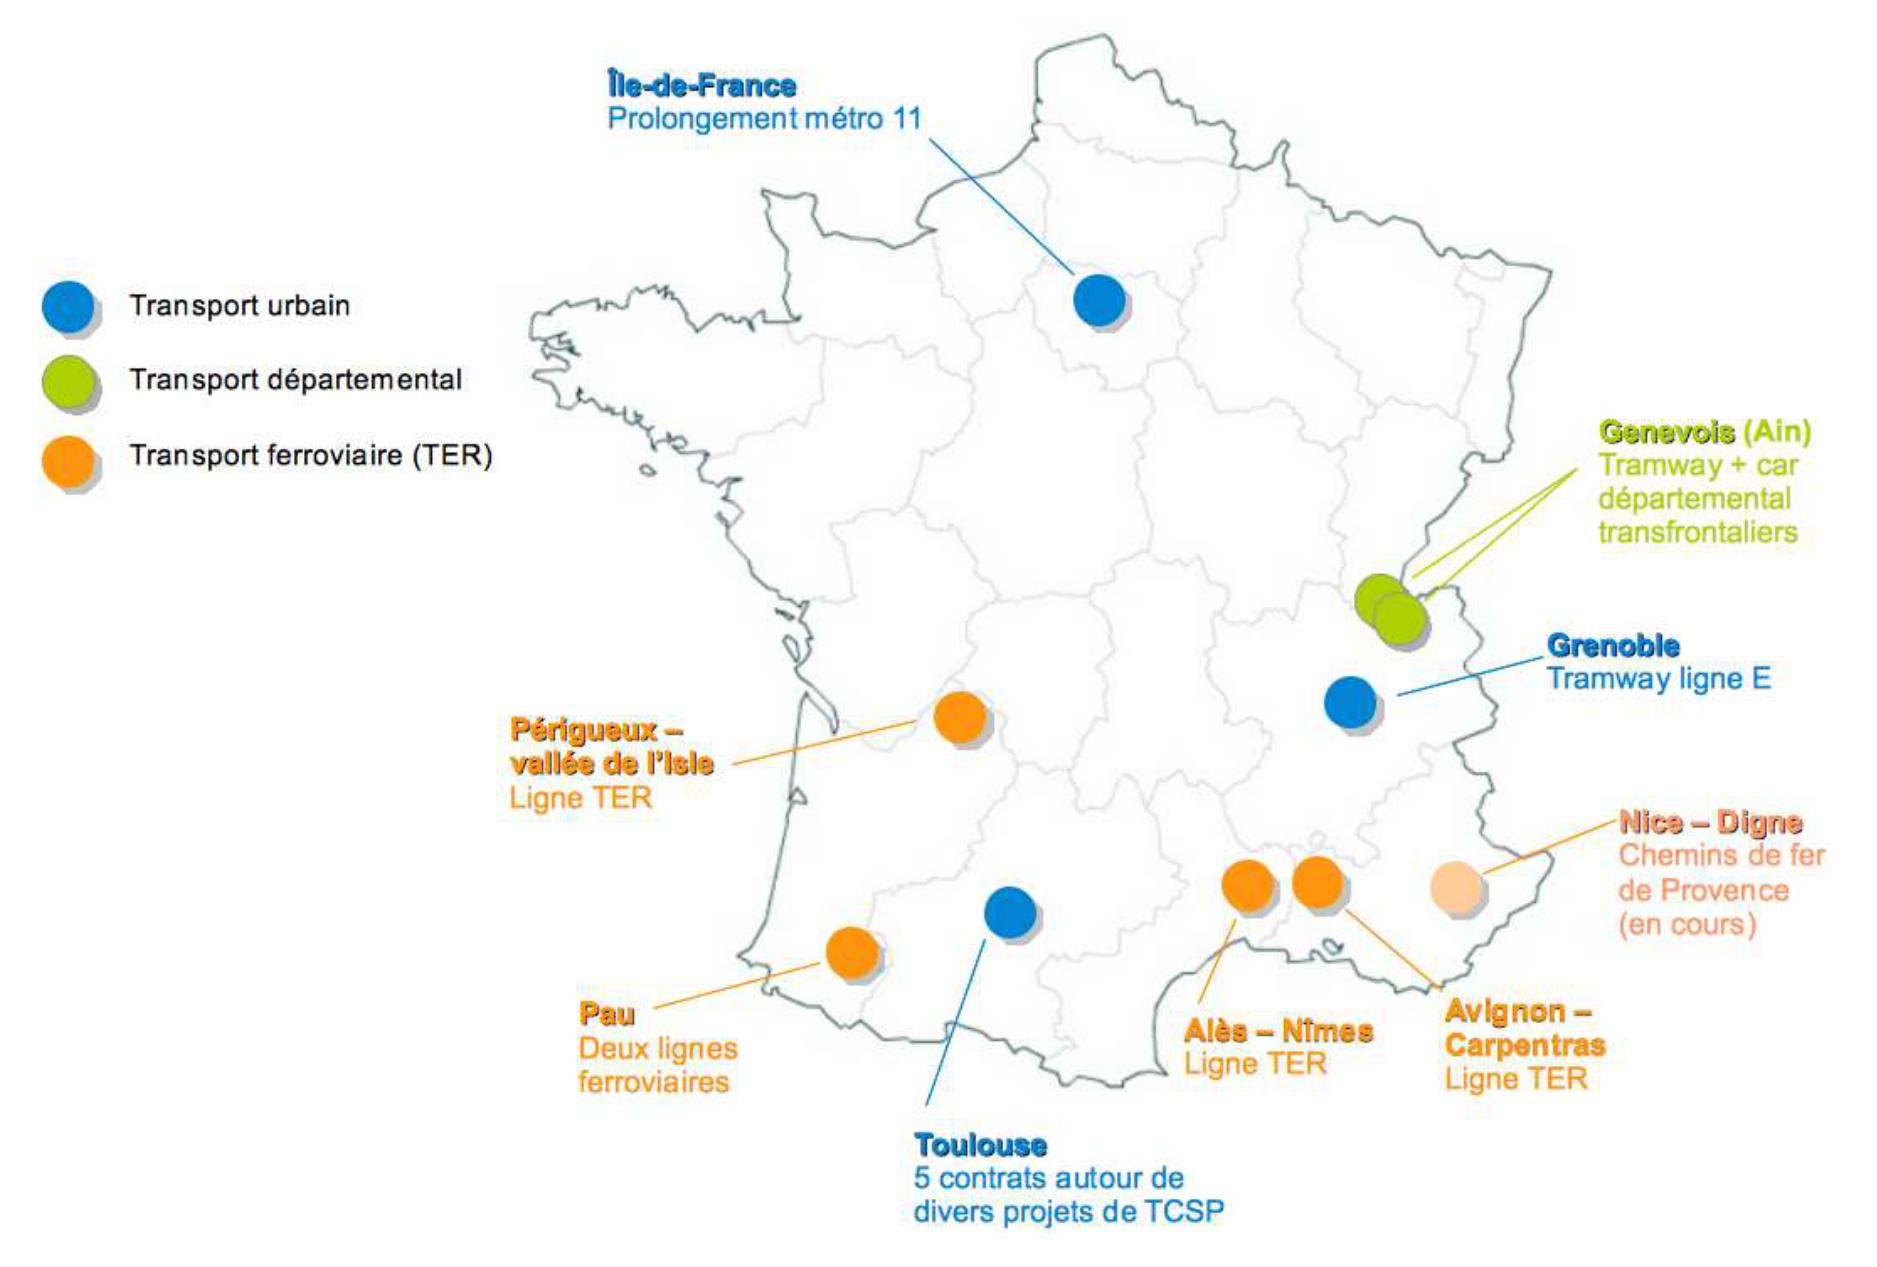
\includegraphics[width=0.75\columnwidth]{src/Figures/Chap-1/Carte_contrats_axe.jpg}}
        \vspace{5pt}
        \begin{flushright}\scriptsize{
        Source: \textcolor{blue}{\textcite[18]{bentayou_contrat_2015}}\index{Bentayou, Gilles|pagebf}\index{Perrin, Emmanuel|pagebf}\index{Richer, Cyprien|pagebf}
        }\end{flushright}
    \end{carte}

% Definition of contrats d'axe
In response to the recommendations made by \textcolor{blue}{\textcite[56]{lhostis_concevoir_2009}}\index{L'Hostis, Alain|pagebf}\index{Alexandre, Elsa|pagebf}\index{Appert, Manuel|pagebf}\index{Araud-Ruyant, Catherine|pagebf}\index{Basty, Marius|pagebf}\index{Biau, Géraldine|pagebf}\index{Bozzani-Franc, Sandra|pagebf}\index{Boutantin, Gratienne|pagebf}\index{Constantin, Chantal|pagebf}\index{Coralli, Monica|pagebf}\index{Durousset, Marie-Jeanne|pagebf}\index{Fradier, Christophe|pagebf}\index{Gabion, Cyrille|pagebf}\index{Leysens, Thomas|pagebf}\index{Mermoud, Françoise|pagebf}\index{Olny, Xavier|pagebf}\index{Perrin, Emmanuel|pagebf}\index{Robert, Jean|pagebf}\index{Simand, Noémie|pagebf}\index{Stransky, Vaclav|pagebf}\index{Soulas, Claude|pagebf}\index{Verdier, Anne-Marie|pagebf}\index{Vulturescu, Bogdan|pagebf} on the importance of creating a dialogue space dedicated to coordinating urban planning and transport\footnote{~
    In their French-German action-research report \textsl{Bahn.Ville 2}, \textcolor{blue}{\textcite[56]{lhostis_concevoir_2009}}\index{L'Hostis, Alain|pagebf}\index{Alexandre, Elsa|pagebf}\index{Appert, Manuel|pagebf}\index{Araud-Ruyant, Catherine|pagebf}\index{Basty, Marius|pagebf}\index{Biau, Géraldine|pagebf}\index{Bozzani-Franc, Sandra|pagebf}\index{Boutantin, Gratienne|pagebf}\index{Constantin, Chantal|pagebf}\index{Coralli, Monica|pagebf}\index{Durousset, Marie-Jeanne|pagebf}\index{Fradier, Christophe|pagebf}\index{Gabion, Cyrille|pagebf}\index{Leysens, Thomas|pagebf}\index{Mermoud, Françoise|pagebf}\index{Olny, Xavier|pagebf}\index{Perrin, Emmanuel|pagebf}\index{Robert, Jean|pagebf}\index{Simand, Noémie|pagebf}\index{Stransky, Vaclav|pagebf}\index{Soulas, Claude|pagebf}\index{Verdier, Anne-Marie|pagebf}\index{Vulturescu, Bogdan|pagebf} stress the importance of establishing a commission tasked with bringing together the relevant stakeholders and funding bodies, and developing the tools necessary for its proper functioning. In the fifth action of their report, the authors propose the creation of what they call the \Commas{Urban Planning and Mobility Interfaces Commission (IUD)}.
}, the \textsl{contrat d’axe} is a tool designed to strengthen the articulation between these two areas. The \textsl{contrat d’axe} thus represents an innovative instrument for territorializing the imperatives of this coordination, while illustrating a transformation of public action methods \textcolor{blue}{\autocite[427]{maulat_coordonner_2014}}\index{Maulat, Juliette|pagebf}\index{Beaucire, Francis|pagebf}. In practice, it is a negotiated approach between various partners aimed at defining clear partnership commitments within a framework inspired by the principles of \acrshort{TOD} \textcolor{blue}{\autocite[1]{cerema_outils_2021}}\index{Cerema@\textsl{Cerema}|pagebf}. The \textsl{contrat d’axe} promotes a logic of inter-territoriality, favoring cooperation between actors rather than hierarchy \textcolor{blue}{\autocite[112, 133]{vanier_pouvoir_2008}}\index{Vanier, Martin|pagebf}. This mechanism has a dual role: to create urban regulation and to align a territorial project within a contractual framework, without requiring the institutionalization of new levels of governance \textcolor{blue}{\autocite[11]{cerema_articuler_2010}}\index{Cerema@\textsl{Cerema}|pagebf}. Instead of mobilizing new resources, the \textsl{contrat d’axe} relies on the inventive reuse of available levers of action \textcolor{blue}{\autocite[12]{cerema_articuler_2010}}\index{Cerema@\textsl{Cerema}|pagebf}, seeking to synchronize the timelines between transport projects and urban developments \textcolor{blue}{\autocite[25]{meunier-chabert_contrats_2014}}\index{Meunier-Chabert, Martine|pagebf}. This approach marks an evolution in the design of railway projects, integrating them into a network-based territorial management logic and associating them with local planning projects \textcolor{blue}{\autocites[457, 468]{maulat_coordonner_2014}[94]{maulat_contractualiser_2015}}\index{Maulat, Juliette|pagebf}\index{Beaucire, Francis|pagebf}. Beyond its technical character, the \textsl{contrat d’axe} is a political tool aimed at strengthening the territorial foundation of regions and their position within the railway world \textcolor{blue}{\autocite[93]{maulat_contractualiser_2015}}\index{Maulat, Juliette|pagebf}.%%Translated%%

% Experiences with contrats d'axe
The experiences with \textsl{contrat d’axe} demonstrate a gradual \Commas{bottom-up} shift in practices, fostering new forms of cooperation and placing greater importance on local specificities and political negotiation \textcolor{blue}{\autocite[96]{maulat_contractualiser_2015}}\index{Maulat, Juliette|pagebf}. This generic tool allows for multiple adaptations depending on local contexts \textcolor{blue}{\autocite[457, 468]{maulat_coordonner_2014}}\index{Maulat, Juliette|pagebf}\index{Beaucire, Francis|pagebf}, mobilizing different sectors and scales, from tramway lines to railway ones \footnote{~
    Among the various forms of \textsl{contrats d’axe}, the railway contracts for \acrshort{TER} axes stand out due to their broader spatial scale, which requires the involvement of a larger number of partners \textcolor{blue}{\autocite[51]{cerema_articuler_2015}}. For regions, these contracts are a strategic tool to overcome the traditional \Commas{counter} logic in their relations with local authorities. They help improve communication on the costs and constraints related to railways while highlighting the actions taken in this regard \textcolor{blue}{\autocite[53]{cerema_articuler_2015}}. Moreover, they provide an opportunity to narrate railway and territorial policies \textcolor{blue}{\autocite{fandio_contrat_2023}}\index{Fandio, Cédric|pagebf}\index{Vezinaud, Nathan|pagebf}.
} \textcolor{blue}{\autocite[20]{afoun_mostaganem_2022}}\index{Afoun, Mohammed|pagebf}\index{Belguesmia, Noureddine|pagebf}. The approaches vary in terms of their degree of completion (see \hyperref[fig-chap1:carte-contrats-axe-france]{Map~\ref{fig-chap1:carte-contrats-axe-france}}, page~\pageref{fig-chap1:carte-contrats-axe-france}). For example, advanced contracts or charters have been implemented in Grenoble and Île-de-France, while initiatives are still in the preparatory stage in Lille and Geneva \textcolor{blue}{\autocites[2]{cerema_articuler_2010}[11]{cerema_articuler_2015}}\index{Cerema@\textsl{Cerema}|pagebf}. Whether in Toulouse, Grenoble, or Île-de-France, \textsl{contrats d'axe} have been integrated into the \acrfull{SCoT} and the \acrfull{SDRIF}. In the Occitan metropolitan area, the \acrfull{SCoT} introduced \Commas{urban-planning-transport coherence zones,} followed by \Commas{urban pacts,} aiming to intensify urbanization along existing or future corridors of major transport lines such as the metro, tramway, or \acrshort{BRT} \textsl{Linéo} \textcolor{blue}{\autocites[49]{toulouse_metropole_plui-h_2019}[26]{meunier-chabert_contrats_2014}[3]{cerema_outils_2021}}\index{Toulouse Métropole@\textsl{Toulouse Métropole}|pagebf}\index{Meunier-Chabert, Martine|pagebf}\index{Cerema@\textsl{Cerema}|pagebf}. In the Alpine agglomeration, the first \textsl{contrat d’axe} supports the commissioning of the tramway line E. This contract sets objectives for housing supply, public space requalification, and updates to the \acrfull{PLU} of the involved municipalities to incorporate urban intensification principles \textcolor{blue}{\autocites[3]{aurg_contrat_2022}[2]{cerema_outils_2021}}\index{AURG@\textsl{AURG}|pagebf}\index{Cerema@\textsl{Cerema}|pagebf}. The \Commas{territorial development contract} in Île-de-France, meanwhile, is part of the 2010 Grand Paris law framework. It supports the creation of new stations for the \textsl{Grand Paris Express} while facilitating their integration into regional planning projects \textcolor{blue}{\autocite[19]{cerema_articuler_2015}}\index{Cerema@\textsl{Cerema}|pagebf}. In the Lille metropolitan area, the \acrshort{DIVAT}\footnote{~
    Three main categories of \acrfull{DIVAT} have been identified, among the stops with more than ten daily crossings in each direction. Each category is associated with specific planning recommendations \textcolor{blue}{\autocite[23]{cerema_articuler_2010}}:
        \begin{customitemize}
    \item The \acrshort{DIVAT} of \Commas{level 1} includes the so-called \Commas{urban} \acrshort{TER} stops as well as metro and tram stations;
    \item The \acrshort{DIVAT} of \Commas{level 2} applies to \Commas{suburban} \acrshort{TER} stops and \Commas{urban} \acrshort{BRT} stations;
    \item The \acrshort{DIVAT} of \Commas{level 3} covers \Commas{suburban} \acrshort{TER} and \acrshort{BRT} stops.
        \end{customitemize}
    In 2010, 120 \acrshort{DIVAT} were listed, covering a third of the metropolitan population and a tenth of the total territory area \textcolor{blue}{\autocite[18]{cerema_articuler_2010}}. The \acrshort{DIVAT} aim to establish minimum density objectives for any new residential or commercial construction \textcolor{blue}{\autocite[19]{lmcu_plan_2011}}. They also specify parking standards, accessible pedestrian routes including accommodations for people with reduced mobility, and secure bike parking spaces installed every two to three metro or tram stations, in line with the cycling network \textcolor{blue}{\autocite[19]{lmcu_plan_2011}}.
}, integrated into the \acrfull{PLUi} and derived from the revision of the \acrshort{PDU}, define intervention areas within a 500-meter radius around \acrshort{TER} stations, metro, tram, and \acrshort{BRT} stations \textsl{Liane} \textcolor{blue}{\autocites[19]{lmcu_plan_2011}[26]{meunier-chabert_contrats_2014}}\index{Meunier-Chabert, Martine|pagebf}\index{Métropole Européenne de Lille@\textsl{Métropole Européenne de Lille}|pagebf}. Unlike the previous cases, this approach is managed by a unified authority, consolidating urban planning and transport competencies within the same administrative area \textcolor{blue}{\autocite[3]{cerema_articuler_2010}}\index{Cerema@\textsl{Cerema}|pagebf}.%%Translated%%

% Results and limitations
Due to their recent emergence, few studies have yet evaluated the outcomes of \textsl{contrats d’axe}, particularly those related to railways \textcolor{blue}{\autocite{fandio_contrat_2023}}\index{Fandio, Cédric|pagebf}\index{Vezinaud, Nathan|pagebf}. While most initiatives are still in development, these initial efforts can already be considered positive, according to \textcolor{blue}{\textcite[17-18]{cerema_articuler_2015}}\index{Cerema@\textsl{Cerema}|pagebf}. The contributions of the \textsl{contrats d’axe} manifest at several levels: the effective establishment of a dialogue and cross-disciplinary work space around transport corridors, overcoming administrative constraints; facilitating the development of transport projects; and achieving results in terms of guiding urbanization in line with transport services, with changes to urban planning rules and developments. A notable example is the Grenoble \textsl{contrat d’axe}, signed ten years ago, which achieved its goals: over 6,000 housing units were built along the strategic route, and the anticipated reduction in car traffic exceeded projections \textcolor{blue}{\autocites[7]{aurg_contrat_2022}[2]{cerema_outils_2021}}\index{AURG@\textsl{AURG}|pagebf}\index{Cerema@\textsl{Cerema}|pagebf}. Despite these encouraging results, several limitations still hinder the impact of \textsl{contrats d’axe}:
    \begin{customitemize}
\item \textsl{Institutional complexity and political orientation}. The \textsl{contrat d’axe} does not reduce the complexity related to the division of responsibilities between local authorities and decision-making levels, as demonstrated by \textcolor{blue}{Juliette} \textcolor{blue}{\textcite[469]{maulat_coordonner_2014}}\index{Maulat, Juliette|pagebf}\index{Beaucire, Francis|pagebf} in her doctoral thesis on the need for coordination between networks and territories in practice. It is more of a pragmatic tool for managing and regulating the gaps between institutional boundaries and territorial issues \textcolor{blue}{\autocite[96]{maulat_contractualiser_2015}}\index{Maulat, Juliette|pagebf}. While it opens up possibilities for better coordination, this instrument mainly functions as a governance and political communication tool, aimed at legitimizing a project \textcolor{blue}{\autocite[84]{gachon_impact_2019}}\index{Gachon, Mickaël|pagebf}. Unlike \acrshort{TOD}, which is more focused on technical programming and urban production, the \textsl{contrat d’axe} aims to reinvent a coordinated governance of transport and urban planning policies to address the dissociation of steering logics \textcolor{blue}{\autocites[118]{bentayou_contrat_2015}[20]{afoun_mostaganem_2022}}\index{Bentayou, Gilles|pagebf}\index{Perrin, Emmanuel|pagebf}\index{Richer, Cyprien|pagebf}\index{Afoun, Mohammed|pagebf}\index{Belguesmia, Noureddine|pagebf}. This approach thus requires significant investment in cross-disciplinary facilitation, typically managed by urban planning agencies \textcolor{blue}{\autocite[2]{cerema_outils_2021}}\index{Cerema@\textsl{Cerema}|pagebf};
\item \textsl{Non-binding nature}. These mechanisms have no legal standing in the \textsl{Urban Planning Code}, so the commitments made by the signatory partners are not subject to any legal obligations and do not have enforceable power \textcolor{blue}{\autocite[2]{cerema_outils_2021}}\index{Cerema@\textsl{Cerema}|pagebf}. Therefore, it is necessary to ensure that these commitments are reflected in prescriptive tools such as the \acrshort{PLU}, while fostering a collective dynamic of voluntary commitment. However, further exploration is needed to determine how this mechanism can be effectively integrated into existing operational planning tools, especially at the scale of micro-projects \textcolor{blue}{\autocite[53]{cerema_articuler_2015}}\index{Cerema@\textsl{Cerema}|pagebf}. Due to its limited scope, certain issues, often sensitive ones such as reducing car space, limiting urbanization in areas poorly served by public transport, or reorganizing rail services, are not addressed \textcolor{blue}{\autocite[96]{maulat_contractualiser_2015}}\index{Maulat, Juliette|pagebf}. These findings call for the design of a new generation of \textsl{contrats d’axe}, more binding on the urban aspect and focused on complex transformations, such as train-bike \gls{intermodality} \textcolor{blue}{\autocite[17]{haro_ligne_2021}}\index{Haro, Florent|pagebf}\index{Duvic, Nicolas|pagebf}. Furthermore, in the absence of a legal framework, there is a risk that these mechanisms remain limited to commitments of low scope, incapable of influencing the content or implementation methods of projects. On the contrary, they could become mere feasibility studies without a guarantee of implementation, turning into simple \textsl{gentlemen’s agreements} with no real enforceable power \textcolor{blue}{\autocite[53]{cerema_articuler_2015}}\index{Cerema@\textsl{Cerema}|pagebf};
\item \textsl{Continuity of methods}. The final limitation of \textsl{contrats d’axe} lies in the lack of renewal of practices. This project mechanism maintains sectoral logics and concentrates decision-making powers among public or parapublic actors, excluding \textsl{de facto} private stakeholders such as landowners, operators, or real estate developers \textcolor{blue}{\autocites[96]{maulat_contractualiser_2015}[2]{cerema_outils_2021}}\index{Maulat, Juliette|pagebf}\index{Cerema@\textsl{Cerema}|pagebf}. Unlike the more entrepreneurial \acrshort{TOD} common in the United States or Japan, the French \textsl{contrat d’axe} does not position itself as a \textsl{territorial marketing} tool aimed at attracting populations and investments to valued and competitive territories \textcolor{blue}{\autocite[120]{bentayou_contrat_2015}}\index{Bentayou, Gilles|pagebf}\index{Perrin, Emmanuel|pagebf}\index{Richer, Cyprien|pagebf}.%%Translated%%
    \end{customitemize}

% Transition
The incredible international diffusion capacity of \acrshort{TOD} is both a strength and a limitation of this planning concept, as it is by nature very composite and heterogeneous in its implementations \textcolor{blue}{\autocite[49]{bentayou_transit-oriented_2015}}\index{Bentayou, Gilles|pagebf}. In presenting this theoretical framework, we have chosen to outline the main model of its application in the French context, through the \textsl{contrats d’axe} that have been adopted and adapted. We could have focused on some international case studies of \acrshort{TOD} \textcolor{blue}{\autocite[6]{knowles_transports_2020}}\index{Knowles, Richard~D.|pagebf}\index{Ferbrache, Fiona|pagebf}\index{Nikitas, Alexandros|pagebf}, but we deliberately chose not to address them, given the many existing studies on the subject. These international examples, which reflect the diversity of \acrshort{TOD} adaptations since its formalization, will be discussed in more detail in the next section. We will then focus on recent developments and adaptations of this model, related to our research topic: the issue of \Commas{first and last miles,} and in particular the solutions provided by bicycles, in connection with train stations and their urban environment, to address the shortcomings of car-centered systems.%%Translated%%

% 1.1.3.2.
\needspace{1\baselineskip} % Reserve space
\subsubsection*{Main Adaptations and Renewal of \textsl{Transit-Oriented Development}
    \label{chap1:tod-presentation-generale-declinaisons-hybrids}
    }

    % Introduction Transit Metropolises
In this final subsection, which serves as a transition to the introduction of bicycles and their close relationship with \acrshort{TOD}, we aim to trace the evolution of what mobility and urbanism expert and consultant \textcolor{blue}{Robert} \textcolor{blue}{\textcite[11]{cervero_transit_1998}}\index{Cervero, Robert|pagebf}, in his book \foreignlanguage{english}{\textsl{Transit Metropolis: A Global Inquiry}}, refers to as the concept of \Commas{\textsl{Transit Metropolises}}. These territories, characterized by metropolitanization structured around public transport networks, indeed represent the practical implementation of \acrshort{TOD} principles, often predating its conceptual formalization. They are metropolitan areas that have successfully combined urban forms and mobility systems \textcolor{blue}{\autocite[132]{cervero_transit_2020}}\index{Cervero, Robert|pagebf}. This typology of \Commas{success stories} illustrates, in a deductive manner, how these territories have simultaneously adopted and influenced the adaptable directions of \acrshort{TOD} \textcolor{blue}{\autocite[134]{wheeler_transit_2000}}\index{Wheeler, Stephen~M.|pagebf}. To do so, the author identifies four major adaptations of this planning concept on a global scale: \Commas{adaptive cities}, \textsl{Adaptive Cities}, \Commas{adaptive public transport networks}, \textsl{Adaptive Transit}, \Commas{strong-core cities}, \textsl{Strong-core cities}, and \Commas{hybrid models}, \textsl{Hybrids}, which highlight the inventive ways in which \acrshort{TOD} policies materialize depending on the urban legacies specific to each local context.%%Translated%%

% 1 : Adaptive Cities
First, \textsl{Adaptive Cities} have relied, or continue to rely, on the early development of public transport services that condition the structuring of dense and mixed territories to control urban growth. By anticipating this growth at the metropolitan scale, the goal is to preserve a \Commas{green belt} while organizing movement flows through compact, multifunctional satellite cities that are interconnected with the main urban centers (see \hyperref[fig-chap1:schema-transit-metropolis]{Map~\ref{fig-chap1:schema-transit-metropolis}}, page~\pageref{fig-chap1:schema-transit-metropolis}). This specific form of \textsl{Transit Metropolis} relies on a long-term vision, supported by a high-performance and structuring public transport system \textcolor{blue}{\autocite[132]{cervero_transit_1998}}\index{Cervero, Robert|pagebf}. Several \textsl{Adaptive Cities} are recognized as models of best practices related to \acrshort{TOD}. Among them, we can mention the urban growth model of Stockholm's satellite cities from 1945\footnote{~
    Thanks to significant public land reserves, the Swedish capital chose to develop a network of satellite cities to control urban growth, while offering a polycentric metropolitan system \textcolor{blue}{\autocite[p.~109-130 (Chapter~4)]{cervero_transit_1998}}\index{Cervero, Robert|pagebf}. This project envisions Stockholm in the shape of a star, metaphorically described as a \Commas{pearls on a necklace,} connecting satellite communities radially to the urban center via the \textsl{Tunnelbana} metro system \textcolor{blue}{\autocite[111]{pojani_past_2018}}\index{Pojani, Dorina|pagebf}\index{Stead, Dominic|pagebf}\index{Shiftan, Yoram|pagebf}\index{Kamargianni, Maria|pagebf}. The General Plan developed between 1945 and 1952 notably foresaw the commissioning of four, then eight \textsl{Tunnelbana} lines, electrified and with high service frequency \textcolor{blue}{\autocite[4]{knowles_transports_2020}}\index{Knowles, Richard~D.|pagebf}\index{Ferbrache, Fiona|pagebf}\index{Nikitas, Alexandros|pagebf}. Between these satellite cities, preserved natural and agricultural spaces can be found \textcolor{blue}{\autocite[1-63]{strong_planned_1971}}\index{Strong, Ann Louise|pagebf}. The first generation of satellite cities includes emblematic locations such as Vällingby, an internationally recognized prototype \textcolor{blue}{\autocite[23]{gullberg_city-building_2004}}\index{Gullberg, Anders|pagebf}\index{Kaijser, Anne|pagebf}, as well as Farsta, Skärholmen, Järva, and Täby, developed between the 1950s and 1970s. The resulting urban planning relies on the policy called \textsl{Arbete, Bostad, Centrum} (\textsl{ABC-stad}), which aims to integrate the economic and administrative sectors near train stations within pedestrian spaces. Housing, predominantly family-oriented, is located less than one kilometer from the stations \textcolor{blue}{\autocite[112]{pojani_past_2018}}\index{Pojani, Dorina|pagebf}\index{Stead, Dominic|pagebf}\index{Shiftan, Yoram|pagebf}\index{Kamargianni, Maria|pagebf}. This strategy, supported by financial incentives, aims to avoid the formation of \Commas{bedroom suburbs} and ensure efficient flow organization, particularly through bidirectional commuter traffic \textcolor{blue}{\autocites[43]{cervero_sustainable_1995}[22]{gullberg_city-building_2004}}\index{Cervero, Robert|pagebf}\index{Gullberg, Anders|pagebf}\index{Kaijser, Anne|pagebf}. The results of this approach were quickly evident: between 1980 and 1990, Stockholm was the only one of 37 cities worldwide to record a decrease in the modal share of cars. During peak hours, 55\% of commuters travel in one direction, while 45\% travel in the opposite direction, demonstrating the efficiency of the system \textcolor{blue}{\autocites[705]{kenworthy_patterns_1999}[24]{curtis_transit_2009}}\index{Curtis, Carey|pagebf}\index{Renne, John Luciano|pagebf}\index{Bertolini, Luca|pagebf}\index{Kenworthy, Jeffrey~R.|pagebf}\index{Laube, Felix~B.|pagebf}.
}; the \textsl{Finger Plan} of Copenhagen in 1947\footnote{~
    In a similar context to Stockholm after the war, the Danish capital developed a master plan in 1947. This project, supported by a group of architects and urban planners \textcolor{blue}{\autocite[p.~132-153 (Chapter~5)]{cervero_transit_1998}}\index{Cervero, Robert|pagebf}, aimed to consolidate five railway corridors, illustrated by the metaphor of the \textsl{Finger Plan} (\textsl{Egnsplan}) \textcolor{blue}{\autocite[123-128]{teknisk_kontor_for_udvalget_til_planlaegning_af_kobenhavnsegnen_skitseforslag_1947}}\index{Teknisk kontor for udvalget til planlægning af Københavnsegnen@\textsl{Teknisk kontor for udvalget til planlægning af Københavnsegnen}|pagebf}. These five fingers, representing the railway corridors, allow radial connection of over 29 municipalities to the urban center of the metropolis \textcolor{blue}{\autocite[]{fullerton_scandinavia_1991}}\index{Fullerton, Brian|pagebf}\index{Knowles, Richard~D.|pagebf}, marked by the constraint of limited land in the city \textcolor{blue}{\autocites[254]{knowles_transit_2012}[4-6]{the_danish_nature_agency_finger_2015}}\index{Knowles, Richard~D.|pagebf}\index{The Danish Nature Agency@\textsl{The Danish Nature Agency}|pagebf}. Since the adoption of the \textsl{Master Plan} in 1989, urbanization has been strictly limited to a one-kilometer perimeter along the \Commas{fingers.} This measure has preserved the agricultural and natural spaces located between the different corridors \textcolor{blue}{\autocite[224]{vuk_transport_2005}}\index{Vuk, Goran|pagebf}. In the 1990s and 2000s, the project underwent a shift marked by the construction of a sixth \Commas{finger,} introducing a break with the original polycentric model. This new corridor allowed the development of the new city of Ørestad, connected to the metro, in a bid for global competitiveness. However, this shift, part of a more neoliberal agenda, did not challenge the application of \acrshort{TOD} principles in Copenhagen \textcolor{blue}{\autocites[103-105]{majoor_progressive_2008}[254]{knowles_transit_2012}}\index{Knowles, Richard~D.|pagebf}\index{Majoor, Stan|pagebf}.
}; the \textsl{Concept Plan} of Singapore in 1971\footnote{~
    Starting in 1965, when it gained full sovereignty, the city-state of Singapore embarked on an ambitious urban planning project based on a master plan \textcolor{blue}{\autocite[p.~155-179 (Chapter~6)]{cervero_transit_1998}}\index{Cervero, Robert|pagebf}, initially called the \textsl{Ring Plan}. The national housing development agency, the \acrfull{HDB}, began constructing over 600,000 public housing units, most of which were intended for sale \textcolor{blue}{\autocite[167]{guillot_singapour_2007}}\index{Guillot, Xavier|pagebf}. However, it was in 1971, with the revision of the \textsl{Long Range Concept Plan}, that Singapore truly began implementing, over two decades, a public transport-oriented development matrix. The plan includes the construction of a dense network of \acrfull{MRT}, Singapore's metro (\textsl{Sistem Pengangkutan Gerak Cepat}), serving twenty new high-density cities \textcolor{blue}{\autocite[162]{cervero_transit_1998}}\index{Cervero, Robert|pagebf}. The last stage of Singapore's urban planning took place in 1991, with the ratification of the \textsl{Revised Concept Plan}, marked by the ambition to create a \Commas{\textsl{Tropical City of Excellence}}. This plan introduced greater private sector participation in housing development \textcolor{blue}{\autocite[168]{guillot_singapour_2007}}\index{Guillot, Xavier|pagebf}. In this framework, the \textsl{Constellation Plan} was developed, aiming to relocate commercial establishments near \acrshort{MRT} stations \textcolor{blue}{\autocite[362]{richmond_transporting_2008}}\index{Richmond, Jonathan~E.~D.|pagebf}. This urban development is accompanied by strict national policies regulating car ownership and usage. These measures include a quota system to limit the number of vehicles allowed on the road (\textsl{Vehicle Quota Scheme}), as well as disincentive taxes on car ownership. Furthermore, the \textsl{Electronic Road Pricing} system imposes significant charges for the use of road infrastructure and parking \textcolor{blue}{\autocite[162]{joshi_transit-oriented_2017}}\index{Joshi, Rutul|pagebf}\index{Yogi, Joseph|pagebf}\index{Patel, Kavina|pagebf}\index{Darji, Vishal|pagebf}.
}; or the \textsl{Tokyu Method} in Tokyo since at least the interwar period\footnote{~
    The Tokyo approach lies less in the definition of \textsl{Master Plans} than in an entrepreneurial logic driven jointly by the private and public sectors since the late 1920s \textcolor{blue}{\autocite[p.~181-209 (chapter 7)]{cervero_transit_1998}}\index{Cervero, Robert|pagebf}. Although Tokyo is not the only metropolis to have adopted this strategy \textcolor{blue}{\autocite[87]{bertolini_developing_2016}}\index{Bertolini, Luca|pagebf}\index{Chorus, Paul|pagebf}, it developed a unique approach known as \textsl{conglomerate Transit-Oriented Development}, reinforced by the urban growth of the metropolis between 1945 and 1982 \textcolor{blue}{\autocite[28-29]{liu_historical_2024}}\index{Liu, Yudi|pagebf}\index{Manabe, Rikutaro|pagebf}\index{Nitanai, Ryoichi|pagebf}\index{Murayama, Akito|pagebf}. The development of public transport was actively supported by massive private sector investments, with the emblematic example of \textsl{Tokyu Corporation}. Since the early 20\textsuperscript{th} century, this company began acquiring vast land areas in the metropolis with the aim of developing urban projects centered around the railway lines it operated. This strategy, known as the \textsl{Tokyu Method}, is based on capturing land value appreciation by purchasing land before the construction of railway infrastructure. It illustrates an entrepreneurial approach to \acrshort{TOD}, based on a \Commas{win-win} partnership: public authorities play a coordination role, while transport operators ensure profitability not only through passenger fares but also through land speculation. By 2004, the \textsl{Tokyu Corporation} derived only 41\% of its net income from passenger transport, with the rest generated by activities related to land rent and leasing land for housing, commerce, and hotels \textcolor{blue}{\autocite[110]{suzuki_financing_2015}}\index{Suzuki, Hiroaki|pagebf}. This approach contributed to the transformation of urban forms, shifting from a centralized organization to a highly decentralized model. The resulting multimodal neighborhoods allow for significant decongestion of the urban core, once dominated by the old main station of Tokyo \textcolor{blue}{\autocite[29]{liu_historical_2024}}\index{Liu, Yudi|pagebf}\index{Manabe, Rikutaro|pagebf}\index{Nitanai, Ryoichi|pagebf}\index{Murayama, Akito|pagebf}.
} \textcolor{blue}{\autocite[109-209]{cervero_transit_1998}}\index{Cervero, Robert|pagebf}. Further research will enrich this category by adding new examples, including European ones, such as those of Amsterdam and Rome examined in the doctoral thesis of \textcolor{blue}{Merijn} \textcolor{blue}{\textcite[180-206]{martens_adaptive_2006}}\index{Martens, Merijn|pagebf}, as well as those of Paris and Hong Kong \textcolor{blue}{\autocite[4]{knowles_transports_2020}}\index{Knowles, Richard~D.|pagebf}\index{Ferbrache, Fiona|pagebf}\index{Nikitas, Alexandros|pagebf}.%%Translated%%

% Figure Transit Metropolises
\begin{carte}[h!]\vspace*{4pt}
    \caption{Abstract maps of updated \textsl{Transit Metropolises}.}
    \label{fig-chap1:schema-transit-metropolis}
    \centerline{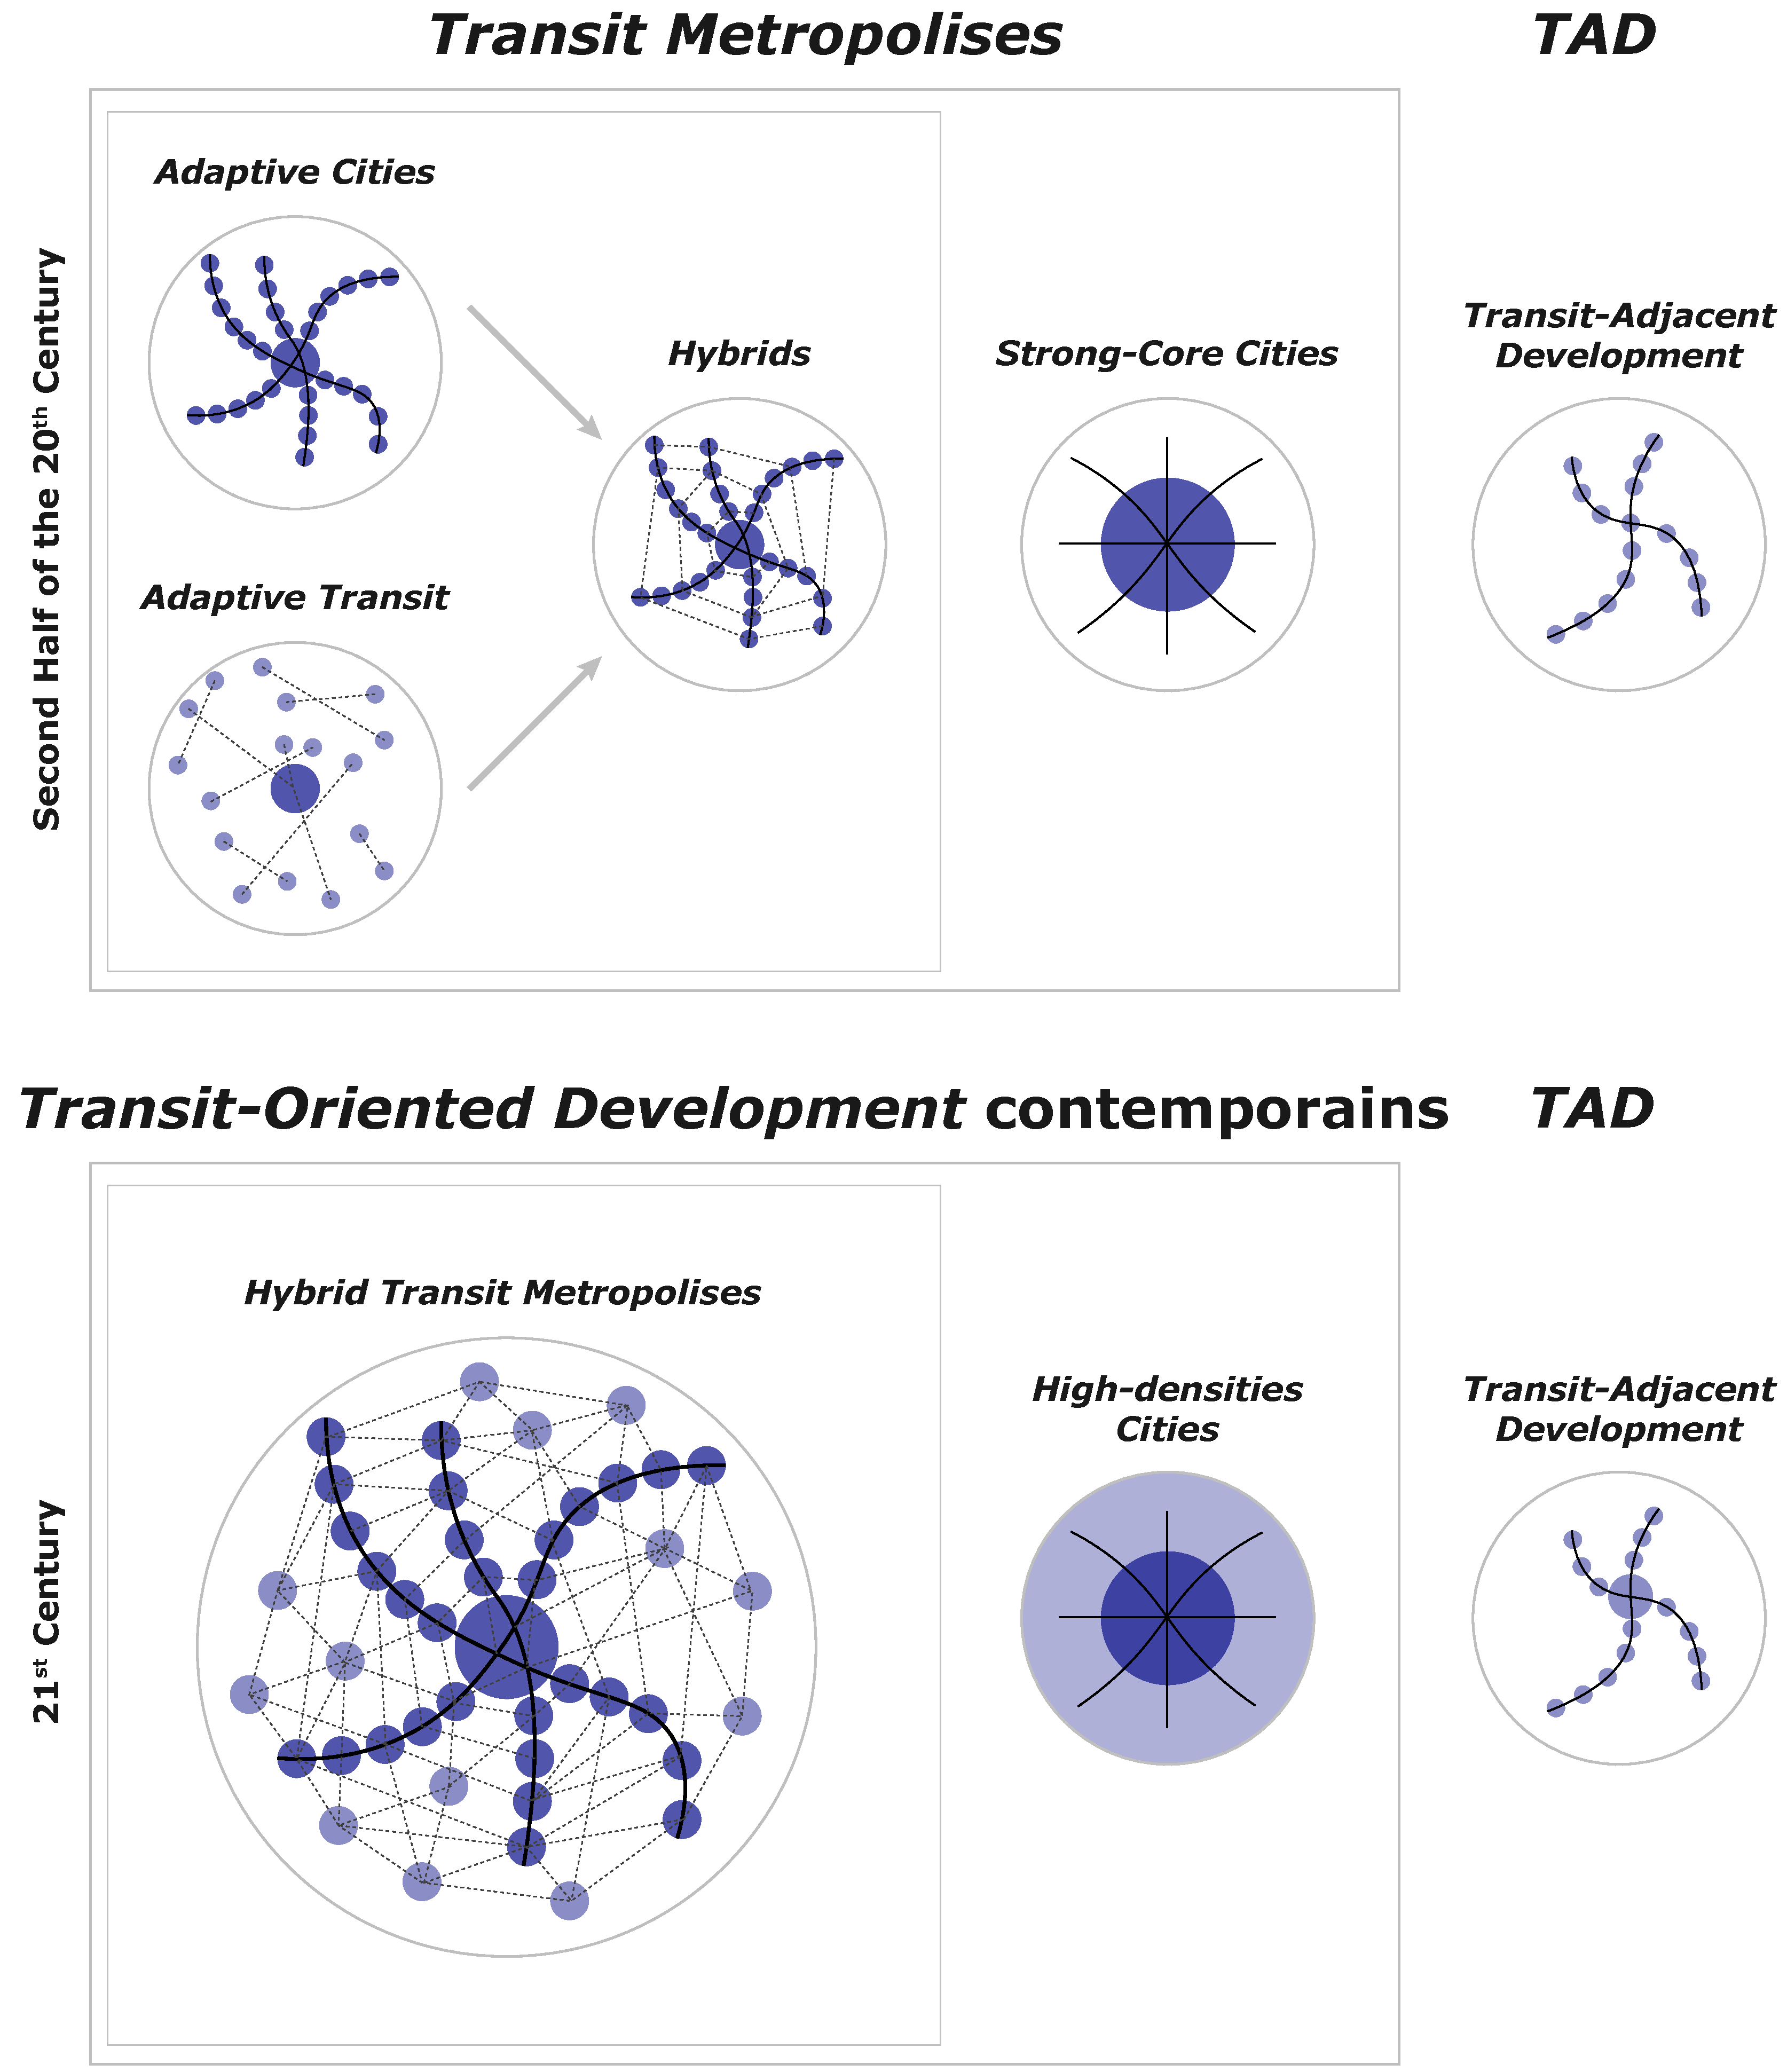
\includegraphics[width=1\columnwidth]{src/Figures/Chap-1/EN_Schema_Alternative_cities_transit.pdf}}
    \vspace{5pt}
    \begin{flushright}\scriptsize{
    Sources: \textcolor{blue}{\textcite[3]{vos_influence_2014}}\index{Vos, Jonas de|pagebf}\index{Acker, Veronique van|pagebf}\index{Witlox, Frank|pagebf} and \textcolor{blue}{\textcite[2]{liu_historical_2024}}\index{Liu, Yudi|pagebf}\index{Manabe, Rikutaro|pagebf}\index{Nitanai, Ryoichi|pagebf}\index{Murayama, Akito|pagebf}
    \\
    Graphic adaptation: \textcolor{blue}{Dylan Moinse (2025)}
    }\end{flushright}
\end{carte}

% Adaptive Transit
\textsl{Adaptive Transit}, characterized by more pronounced urban sprawl, has chosen to reverse the reasoning between urban growth and transport networks. To effectively serve low-density peri-urban areas, mobility systems must adapt to the dispersed urban forms of these spaces. \textcolor{blue}{Susan} \textcolor{blue}{\textcite[108]{handy_reviews_1999}}\index{Handy, Susan|pagebf} highlights this issue, arguing that U.S. cities, heavily marked by urban sprawl, cannot directly replicate the experiences of \textsl{Adaptive Cities} and must instead adopt a model based on \textsl{Adaptive Transit}. In these urban contexts, regional movement follows tangent flows rather than radial ones, connecting the suburbs to each other (see \hyperref[fig-chap1:schema-transit-metropolis]{Map~\ref{fig-chap1:schema-transit-metropolis}}, page~\pageref{fig-chap1:schema-transit-metropolis}). However, conventional public transport networks are often organized around fixed, radial, or sometimes diametrical routes, limiting their capacity to meet these needs. The solutions proposed by this type of \textsl{Transit Metropolis}, also known by the acronym \acrfull{DOT}, rely on technological and service innovations to offer greater flexibility, capable of competing with the private car \textcolor{blue}{\autocite[132]{cervero_transit_2020}}\index{Cervero, Robert|pagebf}. The goal of these systems is to promote alternative mobility to the car-centric model while providing transport services with characteristics similar to those of the car \textcolor{blue}{\autocite[67-68]{bourdin_major_2024}}\index{Bourdin, Alain|pagebf}. These solutions focus on personalized routes, adapted to the challenges of the \Commas{first and last miles} as well as \Commas{door-to-door} mobility needs. These demand-based services complement traditional public transport by enhancing their attractiveness and accessibility. \textsl{Adaptive Transit} can be illustrated by the tram-train system in Karlsruhe, launched in 1992\footnote{~
    Confronted with significant peri-urbanization and a lack of coordination between public transport agencies, the city of Karlsruhe initially struggled to optimize its urban transport network \textcolor{blue}{\autocite[p.~343-360 (Chapter~13)]{cervero_transit_1998}}\index{Cervero, Robert|pagebf}. To address this issue, a context-appropriate project was developed: the design of an interconnected tram-train system, known as the \textsl{Zweisystem-Stadtbahn}. The first line of this system serves the downtown area of Karlsruhe in tram mode, then uses interurban railway tracks to reach Bretten. This project, tested in 1986 before its official launch in 1992, aims to offer an effective solution for peri-urban mobility needs. The commissioning of this pilot line, which quickly saw its frequency increase, achieved its objectives, including a fourfold increase in ridership, mostly former car users \textcolor{blue}{\autocite[41]{beaucire_reseau_2000}}\index{Beaucire, Francis|pagebf}. Beyond its technical aspects, the \Commas{Karlsruhe model} today garners significant interest \textcolor{blue}{\autocite[41]{beaucire_reseau_2000}}\index{Beaucire, Francis|pagebf}. This system provides an effective response to a heterogeneous urban context by efficiently connecting peri-urban areas that had not been integrated into the public transport network before \textcolor{blue}{\autocite[57-65]{grisot_manifeste_2020}}\index{Grisot, Sylvain|pagebf}. This unique technical and fare system allows residents of peri-urban areas to directly reach urban centers without needing to transfer, thus bypassing often remote train stations. At the same time, for local governments and transport operators, this model represents a promise of lower-cost investment through the reuse of existing infrastructure \textcolor{blue}{\autocite[17]{lhostis_multi-criteria_2017}}\index{L'Hostis, Alain|pagebf}\index{Soulas, Claude|pagebf}\index{Vulturescu, Bogdan|pagebf}.
}; the guided bus system in Adelaide, fully operational since 1989\footnote{~
    The city of Adelaide faces a situation similar to Karlsruhe, marked by considerable urban expansion \textcolor{blue}{\autocite[p.~362-377 (Chapter~14)]{cervero_transit_1998}}\index{Cervero, Robert|pagebf}. In response to the rapid urban growth of suburbs to the northeast of the metropolitan area, public authorities initially chose to extend the existing tram network, before turning to an alternative solution: the implementation of a guided bus system. This system, known as the \textsl{O-Bahn}, was the first of its kind in the world and remains the longest network in service today. It constitutes a hybrid between conventional buses and rail transport \textcolor{blue}{\autocite[143]{currie_assessing_2014}}\index{Currie, Graham|pagebf}\index{Delbosc, Alexa|pagebf}. The \textsl{O-Bahn} relies on the use of specific lateral wheels, allowing the \acrshort{BRT} to travel on dedicated, off-road lanes, making the journey both faster and safer \textcolor{blue}{\autocite[2]{currie_bus_2006}}\index{Currie, Graham|pagebf}. This system is designed to efficiently connect the city's \acrfull{CBD} to the new commercial and urban hub of Tea Tree Plaza, located in a rapidly expanding suburb. When it was launched, the \textsl{O-Bahn} had 6 kilometers of tracks in 1986, which were extended to 12 kilometers in 1989. The primary goal was to relieve congestion on the highway network by offering a high-performance, flexible, and relatively low-cost service. The \textsl{O-Bahn} network thus achieves an average commercial speed of 80 kilometers per hour, making it the fastest bus system in the world \textcolor{blue}{\autocite[3]{currie_bus_2006}}\index{Currie, Graham|pagebf}. This success can be attributed to the dedicated infrastructure and the long distance between stops, about five kilometers. Additionally, the occupancy rate of the guided buses is generally twice that of the regular buses in the metropolitan area, while the operating costs per passenger per kilometer are a third lower than those of regular buses \textcolor{blue}{\autocite[7]{basbas_advances_2005}}\index{Basbas, Socrates|pagebf}. Currently, 18 lines use the 12-kilometer alignment, although only 8 of them operate it in its entirety \textcolor{blue}{\autocite[3]{rogers_o-bahn_2002}}\index{Rogers, Lee~H.|pagebf}. This system illustrates how a region faced with significant peri-urbanization chose not to contain this urban dynamic but to connect it to the urban core. The \textsl{O-Bahn} infrastructure is also able to cross dense neighborhoods without requiring significant space reconfigurations. However, despite the system's popular and even tourist success, Adelaide remains dominated by cars. This dominance is also reflected among \textsl{O-Bahn} users, over half of whom drive to the stations, necessitating recurrent expansion of \acrfull{PnR} facilities. These expansions occur despite initial efforts to improve pedestrian and cycling infrastructure around the stations \textcolor{blue}{\autocite[11]{currie_bus_2006}}\index{Currie, Graham|pagebf}.
}; or the \textsl{paratransit} system, called \textsl{microbús}, in Mexico City\footnote{~
    In Mexico City, the significant gap between public transport provision and the extent of the urbanized area has fostered the emergence of self-regulated strategies initiated by the market. It was in this context that the private transport service \textsl{microbús}, also known as \textsl{pesero}, was established in the 1970s. This system developed spontaneously to meet mobility needs in areas not served by the public transport network \textcolor{blue}{\autocite[p.~379-399 (Chapter~15)]{cervero_transit_1998}}\index{Cervero, Robert|pagebf}. Thus, the market adapted to bridge the gap between growing mobility demand and insufficient infrastructure and service provision. Faced with the rapid expansion of Mexico City's urban area, \textsl{paratransit} found its place within the mobility system by coexisting as a transfer mode. This service enables the transportation of isolated populations to public transport stations located on the outskirts of the city center. Operating like collective taxis, these vehicles, often originally cars, follow a fixed route similar to that of a bus line. They pick up and drop off passengers on demand along the \gls{itinerary} \textcolor{blue}{\autocite[4]{chiu_does_2022}}\index{Chiu, Bing-yu|pagebf}. This \Commas{informal} system plays a key role as a self-organized feeder service, as confirmed by the existing literature \textcolor{blue}{\autocite[98, 246]{adjeroud_coexistence_2024}}\index{Adjeroud, Heythem|pagebf}\index{Chapelon, Laurent|pagebf}\index{Lammoglia, Adrien|pagebf}. It notably has the advantage of not necessarily requiring public investment. However, it can represent direct competition to formal public transport and can contribute to urban sprawl \textcolor{blue}{\autocite[4]{chiu_does_2022}}\index{Chiu, Bing-yu|pagebf}. Based on this, \textcolor{blue}{Edzani} \textcolor{blue}{\textcite[65]{libunyu_paratransit-oriented_2024}}\index{Libunyu, Edzani|pagebf} identifies a form of \textsl{Paratransit-Oriented Transit-Oriented Development}, using Mexico City as an example.
} \textcolor{blue}{\autocite[343-399]{cervero_transit_1998}}\index{Cervero, Robert|pagebf}.%%Translated%%

% Hybrids
Deliberately leaving aside the \textsl{Strong-core Cities}, which are based on urban revitalization dynamics and are somewhat distant from our central issue, we focus on the fourth and final type of \textsl{Transit Metropolis}: the \textsl{Hybrids}, which hold particular relevance for our research. Going beyond the dichotomy between \textsl{Adaptive Cities} and \textsl{Adaptive Transit}, these \textsl{Hybrids} stand out by their ability to leverage the strengths of both concepts. This approach seeks to find a balance between dense and mixed urbanism concentrated along well-served corridors and an efficient alternative mobility system designed to cover low-density peripheries. This compromise is illustrated by \hyperref[fig-chap1:schema-transit-metropolis]{Map~\ref{fig-chap1:schema-transit-metropolis}} (page~\pageref{fig-chap1:schema-transit-metropolis}). These \textsl{Hybrids} combine, within a single territory, the mobility and urbanism solutions derived from the two types of \textsl{Transit Metropolis} described earlier. They thus align with a polycentric model, characterized by a hierarchy of interconnected urban centers linked by structuring lines. The accessibility of these centers is enhanced by flexible mobility services that meet the needs of peri-urban and low-density areas \textcolor{blue}{\autocite[213-295]{cervero_transit_1998}}\index{Cervero, Robert|pagebf}.%%Translated

% Hybrid Transit Metropolises
This typology of \textsl{Transit Metropolises}, \textcolor{blue}{Robert} \textcolor{blue}{\textcite[131]{cervero_transit_2020}}\index{Cervero, Robert|pagebf} ultimately reinterprets it under the consolidated designation of \textsl{Hybrid Transit Metropolises}. Such a reinterpretation highlights how these territories have transcended the dichotomy between \textsl{Adaptive Cities} and \textsl{Adaptive Transit}, a duality that has now lost its relevance. This observation refers to the \textsl{Hybrids}, as described by \textcolor{blue}{\textcite[213-295]{cervero_transit_1998}}\index{Cervero, Robert|pagebf} twenty years earlier, although revisited in light of contemporary developments in mobility systems. The determining factor in this revision lies in the emergence and generalization of \acrshort{ICT}, which have simultaneously led to \Commas{smart mobility} and \Commas{smart cities.} Furthermore, the mobility practices and imaginaries of new generations have significantly evolved, influencing travel patterns and accessibility expectations. Behind these concepts, sometimes referred to as \Commas{buzzwords,} \textcolor{blue}{\textcite[137-143]{cervero_transit_2020}}\index{Cervero, Robert|pagebf} advocates for an integrative approach, surpassing the divides in favor of \textsl{Transit Metropolises of the 21\textsuperscript{st} century}. At the conclusion of his analysis, the author observes a convergence of territories toward \textsl{Hybrid Transit Metropolises}, where the mastery of urban forms, aligned with the principles of \acrshort{TOD}, is combined with the development of a range of flexible \Commas{door-to-door} mobility solutions (see \hyperref[fig-chap1:schema-transit-metropolis]{Map~\ref{fig-chap1:schema-transit-metropolis}}, page~\pageref{fig-chap1:schema-transit-metropolis}). These metropolises then integrate \textsl{micro-transit} systems~–~\textcolor{blue}{\textcite[144]{cervero_transit_2020}}\index{Cervero, Robert|pagebf} mentions examples such as walking, cycling, or services like \acrfull{RHS}, \acrfull{PBS}, \acrfull{DBS}, \acrfull{DESS}, \textsl{paratransit}, and autonomous taxis~–~in addition to their \textsl{mass transit} infrastructures \textcolor{blue}{\autocite[7]{thomas_transit-oriented_2020}}\index{Thomas, Ren|pagebf}\index{Bertolini, Luca|pagebf}. At the same time, they adopt a \Commas{smart} demand management (\textsl{smart pricing}). In this regard, the guiding principle of these contemporary \acrshort{TOD}\textcolor{blue}{s} is based on the development of a synergistic multimodal offering, leveraging advances in \acrshort{ICT} and the widespread use of smartphones, with the ultimate goal of reducing car dependence.%%Translated

% Supply and demand approaches
The \textsl{Hybrid Transit Metropolises} rely on structuring elements derived from a dual approach, based on the supply (\acrshort{TSM}) and the demand (\acrshort{TDM}) for mobility, as described by \textcolor{blue}{\textcite[67]{cervero_transit_1998}}\index{Cervero, Robert|pagebf} before being renewed \textcolor{blue}{\autocite[137-143]{cervero_transit_2020}}\index{Cervero, Robert|pagebf}:
    \begin{customitemize}
\item On the one hand, the \acrshort{TSM} approach is based on the \Commas{3Ds}: Density, Diversity, and Design. It also includes the development of non-motorized transportation modes, such as the intermodal use of bicycles. The \acrshort{ICT} play a key role in this dynamic by promising to transform both transportation modalities and the environments in which flows occur. This includes the rise of telecommuting, videoconferencing, and online shopping, as well as optimizing flows through tools such as traffic management via smart signage, vehicle geolocation, real-time passenger data, and automated tolling in urban areas. A notable example is Copenhagen, whose world-renowned cycling network is part of a hybrid \acrshort{TOD} policy. Initially, as we saw, the Danish capital focused on an efficient rail network combined with urban growth concentrated in dense corridors. Later, it developed high-quality cycling infrastructure to accommodate tangential flows in the urban periphery. Bicycles are fully integrated into the \acrshort{TOD} strategy, with abundant bike parking facilities near public transport stations, dedicated cars for carrying bikes on trains, and the development of 26 cycling highways (\textsl{Cycle Super Highways}) totaling more than 500 kilometers. Additionally, \acrshort{PBS} and \acrshort{DBS} services complement this offering;
\item On the other hand, rather than simply aiming to improve mobility at lower costs, the \acrshort{TDM} approach seeks to optimize the use of existing resources by influencing or even reducing the demand for mobility. A growing consensus highlights that managing car parking is one of the most effective demand-based strategies, although it remains sensitive from the perspectives of political negotiations and social acceptability. This approach can take the form of introducing parking fees, developing carpooling, or promoting telecommuting. Complementary measures, such as regulating car use through reduced or banned motorized traffic in certain areas, slowing down traffic, or increasing costs related to car use (fuel, congestion charges, or carbon taxes), further strengthen this approach. Seoul provides a convincing example, where proactive policies in favor of \acrshort{TOD} resulted in the implementation of a 120-kilometer \acrshort{BRT} network in 2017. This initiative was accompanied by the conversion of car-centered neighborhoods into pedestrian spaces \textcolor{blue}{\autocite[6]{prayogi_bus_2018}}\index{Shin, Dooho|pagebf}, with the most emblematic project being the restoration of the Cheonggyecheon river in 2003, which had previously been transformed into an urban highway \textcolor{blue}{\autocite[]{shin_cheongyecheon_2013}}\index{Shin, Dooho|pagebf}.
    \end{customitemize}%%Translated%%

% E-TOD
This reflection on a revision of \acrshort{TOD} principles resonates with the concept of \acrfull{E-TOD}, developed by urban planning and civil engineering researcher \textcolor{blue}{\textcite{schneider_illustrating_2012}}\index{Schneider, Jerry~B.|pagebf}. This concept already envisaged the promise of benefits arising from the integration of technologies to enrich the original urban model. The basic postulate is based on an observation also observable in the \textsl{Transit Metropolises}, particularly in the case of \textsl{Adaptive Transit} and \textsl{Hybrids}. These are territories with a largely sprawling and fragmented urban fabric, poorly served by conventional public transport networks, and which pose the fundamental issue of the \Commas{first and last miles} of public transportation \textcolor{blue}{\autocite[133]{cervero_transit_2020}}\index{Cervero, Robert|pagebf}. To address this, \textcolor{blue}{\textcite[141]{schneider_prt_1992}}\index{Schneider, Jerry~B.|pagebf} proposes a vision of \acrshort{TOD} that pays attention to the function of intermodality and connectivity. This approach would benefit from integrating a moderately capacitative transport system with increased accessibility, embodied by what he calls \acrfull{PRT}\footnote{~
    \acrfull{PRT} is a transport system, often automated and on its own track, which uses individual or low-capacity pods designed to transport individuals or small groups directly to their destination. This mobility service lies between conventional public transport and individual travel modes. The \acrshort{PRT} is a form of demand-responsive transport: travelers select their destination, and the vehicle takes a direct route without intermediate stops, unlike conventional public transport systems with regular stops and fixed schedules. This configuration theoretically reduces waiting and travel times. Furthermore, \acrshort{PRT} requires relatively small land footprints, making it particularly suited to dense urban environments. However, this system also has several limitations. It faces the challenge of integration with existing transport networks, high initial construction costs for infrastructure and dedicated services, and limited capacity, which restricts its efficiency in high-demand contexts. In practice, very few \acrshort{PRT} projects have been implemented and commercialized, with most prototypes remaining experimental.
}. The issue here is not about substituting public transport with \acrshort{PRT}, but rather facilitating access to railway stations for areas beyond the socially acceptable walking distance. The \acrshort{E-TOD} method carries an inter-urban interconnection strategy, combining the mechanisms of a global system \acrfull{F-D-C} designed to link all collective transport modes\footnote{~
    The concept of \acrfull{F-D-C} refers to a transport network structuring strategy based on three complementary functions. This model is frequently used in urban and regional transport planning as it offers a coherent and hierarchical organization of mobility flows. The three main components of this model are as follows:
        \begin{customitemize}
    \item \textsl{Feeding} (\textsl{Feeder}). This function involves infrastructures or services dedicated to collecting passengers from peripheral or distant areas and transporting them to strategic access points on the main network;
    \item \textsl{Distribution}. Once passengers arrive at a multimodal interchange hub, the distribution function involves transporting them to their final destination within denser or more complex urban areas. In this context, \acrshort{PRT} plays a central role in managing this step;
    \item \textsl{Circulation}. Circulation refers to movements within a specific area, independent of central points or main lines. It ensures local mobility, particularly in neighborhoods or residential zones.
        \end{customitemize}
}, with the integration of an organizational system referred to as the \textsl{Urban Oasis}\footnote{~
    The \textsl{Urban Oasis} is a concept developed by U.S. architect \textcolor{blue}{Roxanne} \textcolor{blue}{\textcite{warren_urban_1997}}\index{Warren, Roxanne|pagebf}, which proposes an urban planning model focused on creating green spaces and relaxation areas within densely populated urban zones. This concept is part of a broader reflection on how to reintroduce nature and promote well-being in urban environments, which often feature a predominance of hard surfaces, massive infrastructures, and increased demographic pressure. This vision emphasizes the need to reinstate a human scale in urban spaces sometimes perceived as dehumanized, providing places for rest, leisure, and reconnection with nature, as well as integrating principles of urban ecology. By enhancing the environmental and social qualities of urban spaces, the \textsl{Urban Oasis} aims to improve the quality of life for residents while promoting sustainable and resilient urbanism.
} \textcolor{blue}{\autocite[145]{schneider_prt_1992}}\index{Schneider, Jerry~B.|pagebf}. In sum, the innovative idea of this intermodal system, designed according to the characteristic principles of \acrshort{TOD}, is to propose grouping urban clusters and connecting them to the transport network via the secondary \acrshort{PRT} network, following the \textsl{cluster-and-connect} principle (see \hyperref[fig-chap1:schema-e-tod]{Map~\ref{fig-chap1:schema-e-tod}}, page~\pageref{fig-chap1:schema-e-tod}).%%Translated%%

% E-TOD Diagram
\begin{carte}[h!]\vspace*{4pt}
        \caption{Abstract map of the \textsl{cluster-and-connect} strategy proposed within the framework of \textsl{Extended Transit-Oriented Development}.}
        \label{fig-chap1:schema-e-tod}
        \centerline{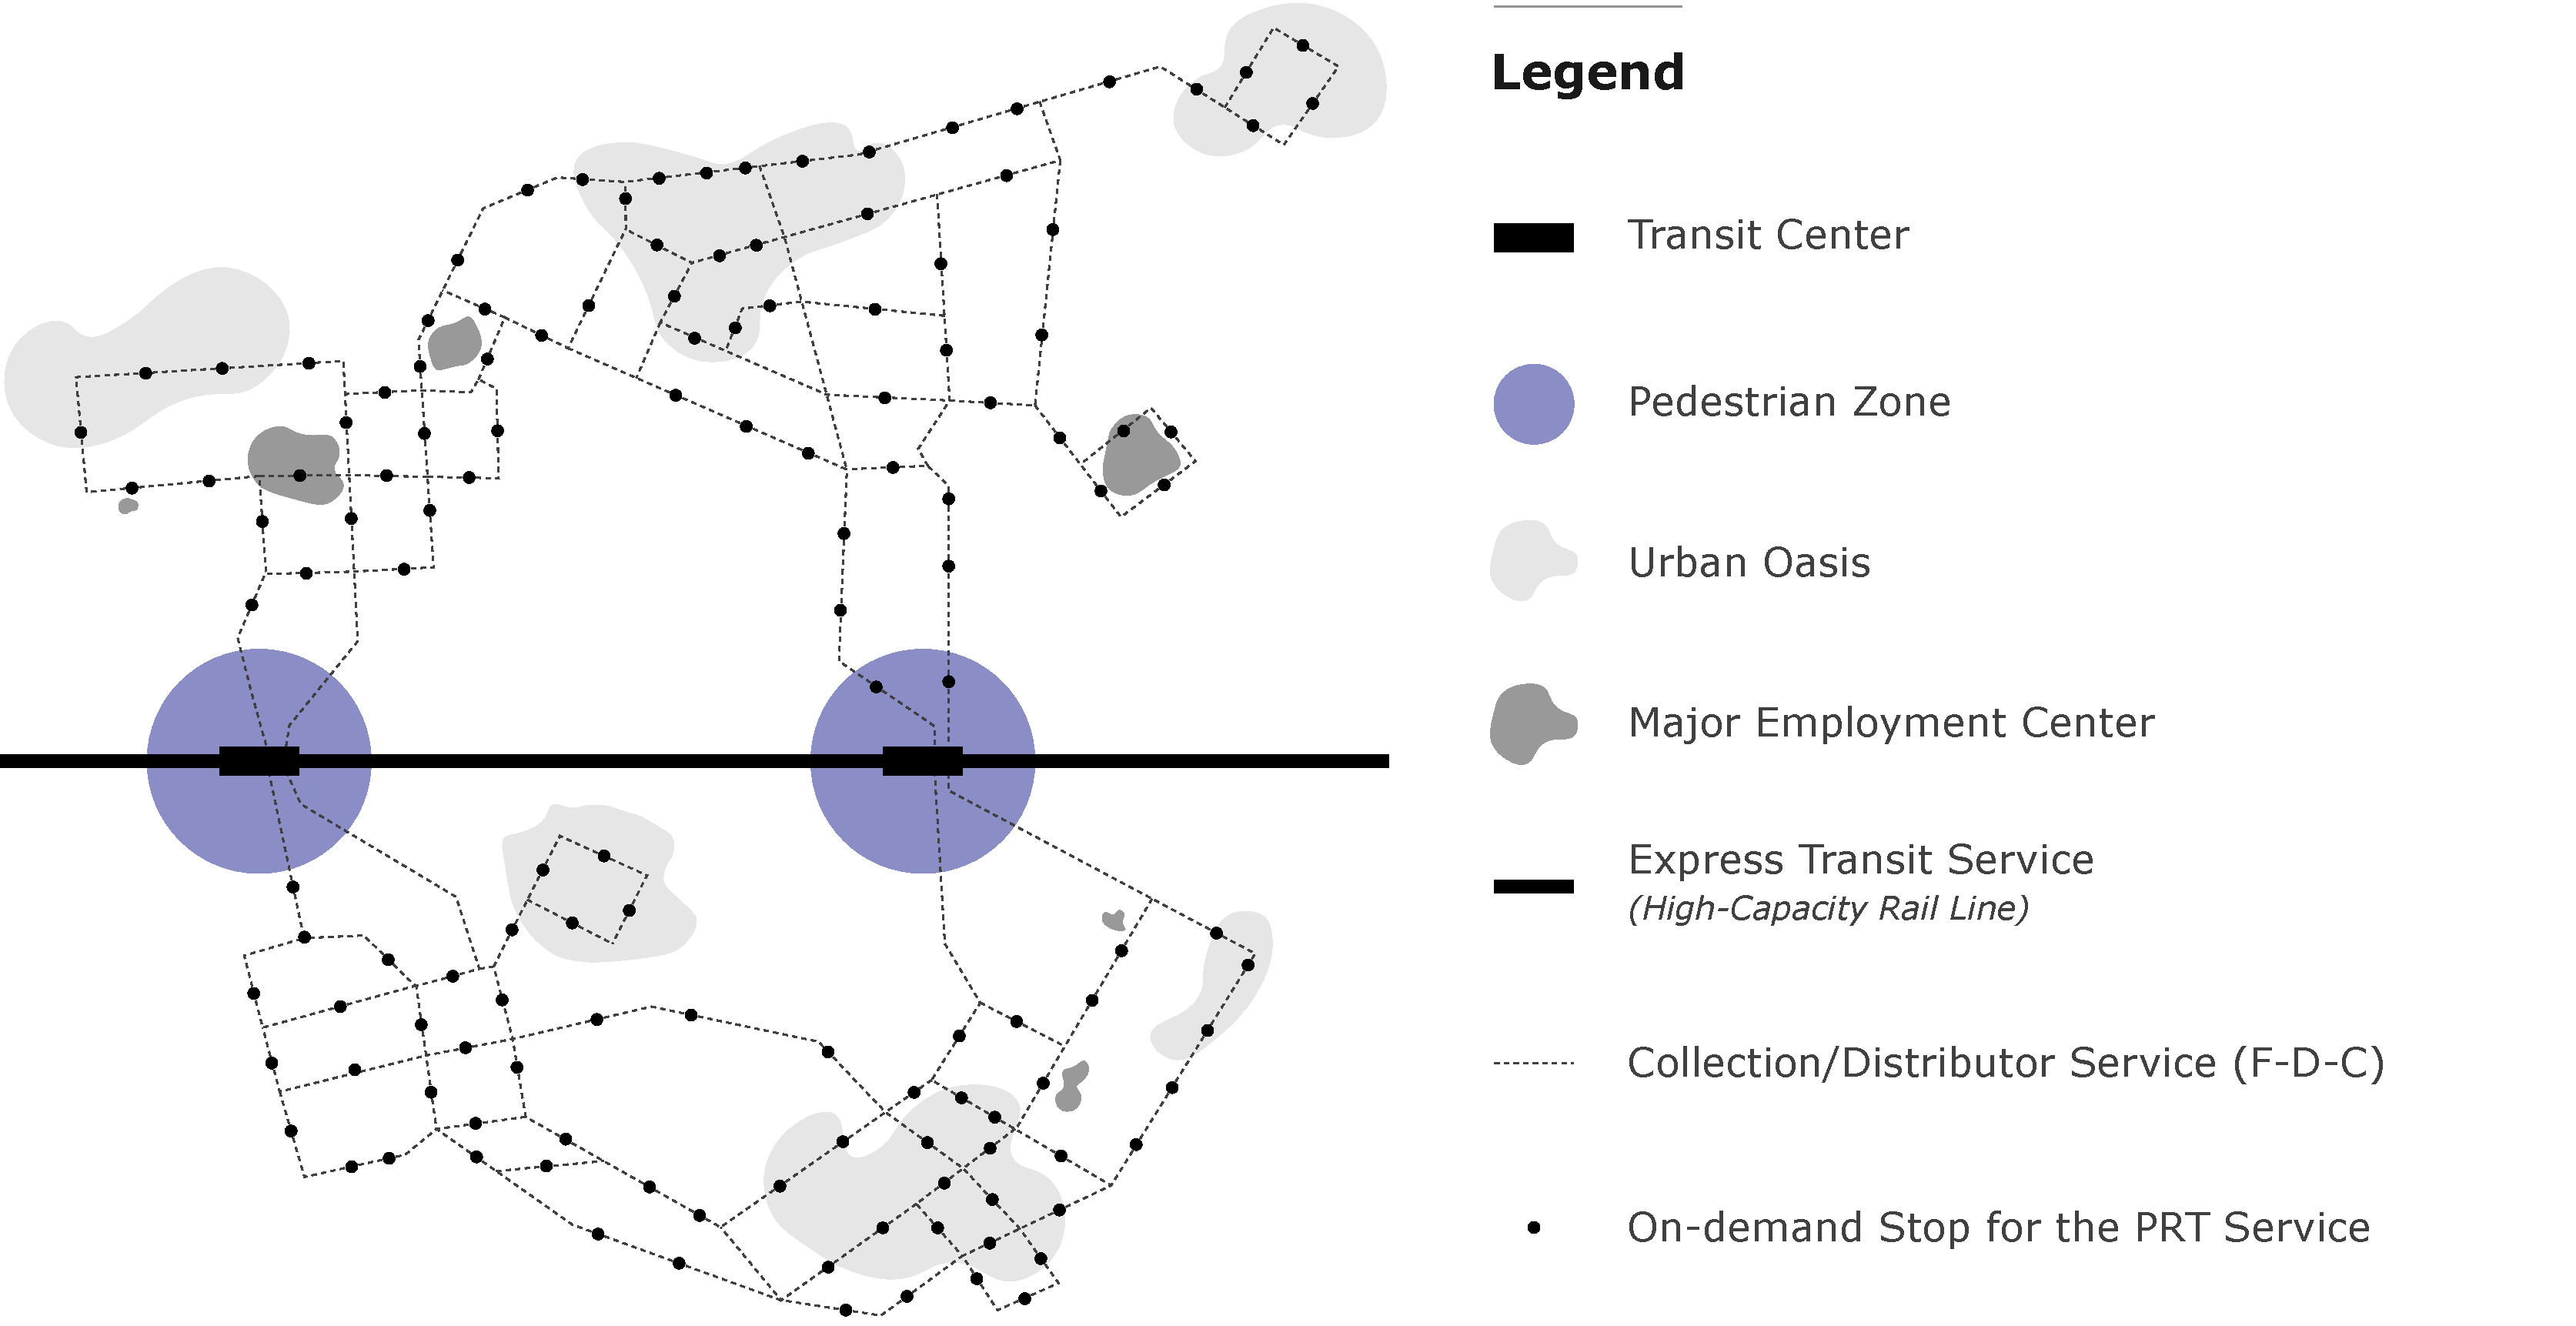
\includegraphics[width=1\columnwidth]{src/Figures/Chap-1/EN_Schema_Schneider.pdf}}
        \vspace{5pt}
        \begin{flushright}\scriptsize{
        Source: \textcolor{blue}{\textcite[142]{schneider_prt_1992}}\index{Schneider, Jerry~B.|pagebf} (see also \textcolor{blue}{\textcite{schneider_illustrating_2012}}\index{Schneider, Jerry~B.|pagebf})
        \\
        Graphic adaptation: \textcolor{blue}{Dylan Moinse (2024)}
        }\end{flushright}
    \end{carte}

% E-TOD Limits and Transition
Nevertheless, this version of \acrshort{TOD}, while maintaining the foundational principles of the model, faces technical, material, and time-related obstacles. The \acrshort{PRT} represents an infrastructural solution that is particularly costly from a budgetary perspective and demanding in terms of implementation timelines. Besides the technological challenges it involves, \acrshort{PRT} struggles to deliver significant gains in terms of congestion reduction, thus undermining its promise of more sustainable mobility and urbanism. For similar reasons, shared autonomous vehicles, which are increasingly featured in projections of a reworked rail-based urbanism, encounter comparable issues, driven by the illusion of a leap in public transport ridership\footnote{~
    In his doctoral thesis, \textcolor{blue}{Félix} \textcolor{blue}{\textcite[333]{carreyre_are_2023}}\index{Carreyre, Félix|pagebf}\index{Coulombel, Nicolas|pagebf}\index{Bouillaut, Laurent|pagebf} focused on evaluating the performance of services based on automated vehicles using a cost-benefit analysis framework combined with multi-agent modeling with \textsl{MATSim}. His work, conducted in the contexts of Berlin and Paris, demonstrated that the introduction of autonomous taxis could worsen congestion in Berlin. Moreover, in the case of Saclay, an intermodal scenario combining these services with the rail system would only increase the average occupancy rate of vehicles, although this would come at the expense of bus usage.
}. In this context, bicycles appear as a more agile and concrete solution that has proven itself in various \textsl{Hybrid Transit Metropolises} around the world. This individual mode of transport, inherently \Commas{door-to-door} and demand-driven, proves to be not only complementary to \acrshort{TOD}, but also much less costly in both economic and temporal terms. Moreover, its integration into urban mobility policies relies on relatively light and adaptable infrastructures. In this perspective, a survey conducted by \textcolor{blue}{\textcite[119]{goletz_intermodality_2020}}\index{Goletz, Mirko|pagebf}\index{Haustein, Sonja|pagebf}\index{Wolking, Christina|pagebf}\index{L'Hostis, Alain|pagebf} in Berlin, Copenhagen, Hamburg, and Paris supports the intermodal potential of cycling within a rail-oriented urbanism. The results show that specialists and researchers interviewed attribute the most promising role to cycling for effectively connecting rail infrastructures, with the notable exception of Paris, where intermodality with urban public transport networks is more widely favored. Building on the thesis of \textsl{Hybrid Transit Metropolises}, profoundly renewed by innovations in mobility, this doctoral research thus aims to examine the role of cycling as a relevant mobility solution to address the challenges of the \Commas{first and last miles.} In doing so, it also seeks to explore the progressive return of cycling to prominence through its modal diversification, around its variations, as well as the reintroduction of electric scooters, updated by advances in electromobility.%%Translated%%

% ___________________________________________
% 1.2.
\newpage
\needspace{1\baselineskip} % Reserve space
\sectionheader{The Resurgence of Light Individual Mobility}
\section{The (Re)birth of a Family of Lightweight Vehicles Designated as \Commas{Light Individual Mobility}, with Shifting Boundaries
    \label{chap1:mobilite-individuelle-legere}
    }

    % Introduction
This section offers a cross-sectional view of the evolving trajectories of the \Commas{small queen} and the \Commas{new queen}, adopting a historical perspective. It highlights the key moments in the technical and social evolution of these two modes of transport. We will particularly focus on understanding how and why these bicycles, long considered leisure objects, have gradually gained legitimacy—still under construction—in daily mobility practices. This rehabilitation takes place in a context of evolving uses and values, as well as in the context of technical and social innovations related to forms of \Commas{retro-innovation} \textcolor{blue}{\autocite{barthelot_retro-innovation_2018}}\index{Barthelot, Bertrand|pagebf}. Although these two objects share a history marked by cycles of rising popularity and withdrawal, they are experiencing a revival today, driven both by technical advancements and by transformations in urban practices. As \textcolor{blue}{Arnaud} \textcolor{blue}{\textcite[26]{passalacqua_monde_2011}}\index{Passalacqua, Arnaud|pagebf}, university lecturer and co-director of the \acrfull{EUP}, points out, urban mobility is a \Commas{\textsl{world where new solutions are often merely reprises of old forms and which, probably unintentionally, maintains a confusion between the old and the contemporary, the past and the future. By focusing on vehicles more than on systems in their entirety, this world remains confused. The vocabulary used, almost frozen since the 19\textsuperscript{th} century, contributes to reinforcing this confusion}}.%%Translated%%

% Innovation Cycles
This observation provides an opportunity to explore the reflections on \Commas{models} and \Commas{innovation cycles} \textcolor{blue}{\autocite[]{schumpeter_theorie_1911}}\index{Schumpeter, Joseph Aloïs|pagebf}, while placing them in a historical, philosophical, and ethical perspective. The Austrian and American economist \textcolor{blue}{Joseph Aloïs} \textcolor{blue}{\textcite[107]{schumpeter_capitalisme_1942}}\index{Schumpeter, Joseph Aloïs|pagebf} illustrates this dynamic through his famous concept of \Commas{creative destruction}, the engine of economic growth through innovation in products, processes, production methods, markets, or raw materials. He observes that \Commas{\textsl{the history of transportation, from the stagecoach to the airplane} [\dots] \textsl{constitutes other examples of the same industrial transformation process} [\dots] \textsl{which incessantly revolutionizes the economic structure from within, continually destroying its aged elements and continually creating new ones.}}. As the researcher in political philosophy and history of ideas \textcolor{blue}{Thierry} \textcolor{blue}{\textcite{menissier_innovations_2021}}\index{Ménissier, Thierry|pagebf} addresses in his work \textsl{Innovations: A Philosophical Inquiry}, innovation is not limited to responding to pre-existing needs; it also acts on the collective imagination and stimulates interest in the \textsl{different}, in order to support emerging projects. Thus, it is about reflecting on the ways to better articulate the transfer and territorialization of innovations, as well as their implementation. In other words, this involves questioning the conditions of their deployment across all segments of society \textcolor{blue}{\autocite[5]{baron_thierry_2022}}\index{Baron, Nacima|pagebf}. This territorialization of innovations has been studied by \textcolor{blue}{\textcite[13]{castex_prise_2017}}\index{Castex, Élodie|pagebf}\index{Frère, Séverine|pagebf}\index{Groux, Annette|pagebf}, particularly through transport planning. Their study supports the gap between the slow shift of public actors in considering new mobility modes—such as \acrfull{STP}—in urban and mobility management tools, and the rapid evolution of needs and innovations driven by private actors.%%Translated%%

% Outline Announcement
In this section, we will examine the evolution of the bicycle and the scooter, considered both as technical and social objects, as well as their place and usage in various territories, depending on urbanization contexts (\hyperref[chap1:proximite-velo-trottinette]{section on the \Commas{golden age} of these vehicles, followed by their decline and \Commas{comeback}}, page~\pageref{chap1:proximite-velo-trottinette}). From this brief historical digression, we will review the main contemporary innovations that have marked these vehicles, notably their electrification and their sharing model in public spaces (\hyperref[chap1:velo-micromobilite-innovations]{section on the diversification and \Commas{modal hybridization} of bicycles}, page~\pageref{chap1:velo-micromobilite-innovations}). Finally, we will contextualize the revival of the bicycle and the scooter, in their various forms, in a \Commas{liquid} society, driven by generations increasingly inclined towards \gls{multimodality}. This framework will also allow us to propose our own definition of this family of vehicles, by delineating more precise conceptual boundaries. This definition aims to integrate the vehicles we identify as having the greatest strategic potential to strengthen and redeploy the principles of \acrshort{TOD} (\hyperref[chap1:caracterisation-mobilite-individuelle-legere]{section on the characterization of a class of vehicles called \Commas{light individual mobility}}, page~\pageref{chap1:caracterisation-mobilite-individuelle-legere}).%%Translated%%

% 1.2.1.
\needspace{1\baselineskip} % Reserve space
\subsection{Evolution of the Design and the Role of the Bicycle among Utility Travel Modes
    \label{chap1:proximite-velo-trottinette}
    }

    % Introduction
Before becoming fully established as urban transport modes in their own right, bicycles and scooters went through more than a century of evolution, marked by both technical innovations and transformations in mobility practices and imaginaries in Europe. Over time, these cycles have experienced paradigms influenced by the social constructs associated with vehicles \textcolor{blue}{\autocite[13]{heran_retour_2015}}\index{Héran, Frédéric|pagebf}. Successive waves have gradually propelled them into daily mobility practices. This subsection, dedicated to a brief chronology of their evolution, aims to better situate these vehicles in their historical and urban context. To this end, we rely on the sequential reading proposed by French historian and sociologist \textcolor{blue}{Catherine} \textcolor{blue}{\textcite[]{bertho-lavenir_voyages_2011}}\index{Bertho-lavenir, Catherine|pagebf}, structured around four periods in the evolution of cycling practice: \Commas{the age of the velocipede} or the fashionable invention (from 1814 to the 1880s); \Commas{the age of the bicycle} or bourgeois leisure (from the 1880s to 1914); \Commas{the age of the bicycle} embedded in daily and tourist mobility (from 1914 to the 1970s); and \Commas{the age of the automobile} or the bicycle as a sport and leisure activity (since 1970). The intention is to provide a cross-sectional reading of the bicycle and the scooter, which share common origins and similar trajectories. These two families of transport modes have experienced a comparable fate when the modern city, with its spatial-temporal spread and increasing travel speeds, was built around urban forms that became inaccessible and ill-suited for these vehicles.%%Translated%%

% 1.2.1.1.
\needspace{1\baselineskip} % Reserve space
\subsubsection*{\Commas{The Golden Age} of the \Commas{Small Queen}
    \label{chap1:proximite-velo-trottinette-chronologie}
    }

    % Bicycle Bourgeois Leisure
\textsl{The Ages of the Velocipede and the Bicycle}. The origins of the bicycle and scooter can be traced back to the invention of the \Commas{running machine} (\textsl{Laufmaschine}), designed in 1817 by the Baden baron \textcolor{blue}{Karl Drais von Sauerbronn}\footnote{~
    He drew upon the idea of the \Commas{céléripède}, literally \Commas{the fast-walker}, from French engineer \textcolor{blue}{Joseph Nicéphore Niepce} \textcolor{blue}{\autocite{puech_bicyclette_2016}}\index{Puech, Chantal|pagebf}. In reality, some inventions predating the one commonly attributed to the \Commas{father of the bicycle} reveal that the concept of this device, based on the use of the wheel, dates back centuries. Among these predecessors, \textcolor{blue}{Leonardo da Vinci} sketched, around 1490, plans for a wooden machine resembling the modern bicycle. This prototype featured a seat, two wheels, and pedals, already reflecting an idea of mechanized individual transportation \textcolor{blue}{\autocite[9]{hills_bicycle_2004}}\index{Hills, Larry|pagebf}.
}. He sought to develop a \Commas{horse-less carriage} that was both efficient and economical \textcolor{blue}{\autocite[24]{heran_retour_2015}}\index{Héran, Frédéric|pagebf}, with the origin of this idea primarily associated with a shortage of horses due to particularly cold summers. Thus, the roots of the bicycle are closely tied to those of the scooter through their common ancestor, the \Commas{velocipede}, known in France as the draisienne and in England as the \textsl{dandy-horse}\footnote{~
    In 1818, an import patent application for the \Commas{running machine} was filed in France, under the supervision of \textcolor{blue}{Louis-Joseph Dineur}. It was also during this period that the first draisiennes appeared in Paris, accompanied by a notable advertising campaign and public events, such as the first race organized at the Luxembourg Gardens \textcolor{blue}{\autocite[141]{kobayashi_histoire_1993}}\index{Kobayashi, Keizo|pagebf}. At the time, the term \Commas{velocipede} was used pejoratively, especially in the press and in comedic performances. However, this word has endured and is still used today to refer to the wooden bicycle, which has neither pedals nor a transmission chain, and is used by children to learn balance and independence \textcolor{blue}{\autocite[21]{jouenne_quest-ce_2022}}\index{Jouenne, Noël|pagebf}.
} (see \hyperref[fig-chap1:frise-chronologique-velo-trottinette]{Figure~\ref{fig-chap1:frise-chronologique-velo-trottinette}}, page~\pageref{fig-chap1:frise-chronologique-velo-trottinette}). This rudimentary vehicle, consisting of two wheels connected by a wooden frame and powered by foot force, experienced limited success among the bourgeoisie and eventually fell into relative obscurity. Its weight and the instability of its wooden wheels made it impractical. From the late 19\textsuperscript{th} century, the bicycle and scooter took distinct trajectories, marking their own identities. On one hand, the \Commas{Michaudine}, with pedals added to a draisienne as early as 1861, popularized the bicycle among the affluent classes (see \hyperref[fig-chap1:frise-chronologique-velo-trottinette]{Figure~\ref{fig-chap1:frise-chronologique-velo-trottinette}}, page~\pageref{fig-chap1:frise-chronologique-velo-trottinette}), through \textsl{leisure} and sports clubs as well as velodromes \textcolor{blue}{\autocite[15-43]{dauncey_french_2012}}\index{Dauncey, Hugh|pagebf}. This evolution led to the \Commas{véloce}, followed by the \Commas{bicycle} in 1866, the \Commas{Grand-Bi} in 1871, and finally the modern bicycle in 1891 \textcolor{blue}{\autocite[27]{heran_retour_2015}}\index{Héran, Frédéric|pagebf}. On the other hand, the history of the scooter is more fragmented: it initially emerged as a toy for children, as early as 1895. For example, the Swiss company \Marque{Wisa-Gloria AG}, founded in 1882 and specializing in toys, was one of the pioneers in the production of scooters for children \textcolor{blue}{\autocite{schweizerisches_nationalmuseum_draisine_2018}}\index{Schweizerisches Nationalmuseum@\textsl{Schweizerisches Nationalmuseum}|pagebf}. The first scooters, resembling those of today, also appeared around 1895. These toys, made of wood and without motors, were equipped with handlebars and two or three wheels (see \hyperref[fig-chap1:frise-chronologique-velo-trottinette]{Figure~\ref{fig-chap1:frise-chronologique-velo-trottinette}}, page~\pageref{fig-chap1:frise-chronologique-velo-trottinette}). They worked through human energy: one foot rested on the board while the other pushed off the ground to propel the user.%%Translated%%

% Scooter Bourgeois Leisure
In parallel, the first scooter models, intended for the children of wealthy families, inaugurated a wave of two-wheeled scooters marketed just before the Great War \textcolor{blue}{\autocite{jeux_et_compagnie_histoire_2013}}\index{Jeux et Compagnie@\textsl{Jeux et Compagnie}|pagebf}. Although the scooter initially retained a status as a toy, it gradually appealed to a broader audience, reaching children from less privileged social classes \textcolor{blue}{\autocite{historia_trottinette_2013}}\index{Historia@\textsl{Historia}|pagebf}. During the interwar period, metallic models with pneumatic tires appeared and were patented, incorporating technical innovations inspired by those of the bicycle \textcolor{blue}{\autocite{arte_histoire_2014}}\index{Arte@\textsl{Arte}|pagebf}. In terms of their relationship with the social world, both the bicycle and the scooter were initially associated with bourgeois practices\footnote{~
    Although the initial development of the bicycle was driven by the upper classes, these groups experienced a sense of injustice linked to a lack of legitimacy on the road. In his doctoral thesis on the history of road usage, \textcolor{blue}{Jean} \textcolor{blue}{\textcite[126-132, 327]{orselli_usages_2008}}\index{Orselli, Jean|pagebf} highlights the challenges faced by cyclists at the end of the 19\textsuperscript{th} century. These difficulties were manifested through regulations marked by a true \Commas{velophobic rage}, as well as popular violence, particularly in rural areas, between 1874 and 1896. These tensions preceded the establishment of national regulations on velocipedes, whose application by municipalities, however, remained largely ignored. This conflict must be understood in the context of a road historically dominated by horse-drawn carriages, which held an ancestral position and enjoyed tacit respect, both from the population and the police. This situation reflects the difficult social acceptance of the bicycle in a society where the horse-drawn carriage still embodied, at the time, a prestigious means of transportation, used by the French aristocracy for centuries \textcolor{blue}{\autocite[139]{orselli_usages_2008}}\index{Orselli, Jean|pagebf}.
}. High prices and social codes reserved them for an elite seeking new leisure and exclusive sports \textcolor{blue}{\autocite[90]{bravard_cercle_2011}}\index{Bravard, Alice|pagebf}. However, with the modernization of manufacturing processes and the democratization of these objects\footnote{~
    The Japanese historian \textcolor{blue}{Keizo} \textcolor{blue}{\textcite[149]{kobayashi_histoire_1993}}\index{Kobayashi, Keizo|pagebf}, in his work titled \textsl{History of the Velocipede from Drais to Michaux 1817-1870: Myths and Realities}, sheds light on the origin of the bicycle by stating that \Commas{\textsl{among the main flaws of the velocipede, it was criticized for the fatigue it caused, its lack of balance while in motion or at rest, and the discomfort from the vibrations.}} In response to these limitations, various technical solutions were considered to alleviate the physical effort and improve the user experience. Improvement inventions multiplied, ranging from enhancing energy transmission by improving traction with the front wheel and propulsion with the rear wheel, to the link chain with gears in 1829, the addition of solid rubber tires in 1869 \textcolor{blue}{\autocites{inpi_draisienne_2020}[38]{jouenne_quest-ce_2022}}\index{Jouenne, Noël|pagebf}\index{INPI@\textsl{INPI}|pagebf}, and the invention of the pneumatic tire with an air chamber in 1888 \textcolor{blue}{\autocite[14]{papon_retour_2012}}\index{Papon, Francis|pagebf}. However, the advances in the velocipede were not solely technical. Its social and cultural development was largely supported by popular events, such as public demonstrations and cycling races, which helped increase its visibility and contributed to its gradual adoption by a wider public.
}, the bicycle and scooter eventually expanded to lower social classes, gradually losing their status as social distinction objects, characteristic of a \Commas{bourgeois culture}.%%Translated%%

% Bicycle Popularization
\textsl{The Age of the Bicycle}. During the Belle Époque and even more so during the Roaring Twenties, cycle tourism became a popular activity in Europe, particularly through the organization of bicycle tours taking the form of weekend itinerant camps \textcolor{blue}{\autocite[26]{eskenazi_voir_2022}}\index{Eskenazi, Manon|pagebf}, as well as with the arrival of the first paid vacations in 1936 \textcolor{blue}{\autocite[108]{dauncey_french_2012}}\index{Dauncey, Hugh|pagebf}. Cyclists could then park their bicycles at inns overnight, a practice that spread particularly in Germany \textcolor{blue}{\autocite[327]{herlihy_bicycle_2004}}\index{Herlihy, David|pagebf}. Between 1918 and the 1950s, the modern bicycle became popular among the working classes, inaugurating a major social innovation: daily bicycle commuting, now seen as a realistic alternative \textcolor{blue}{\autocite[31]{jouenne_quest-ce_2022}}\index{Jouenne, Noël|pagebf}. These commuting trips, especially those of workers, helped reduce travel times while offering more free time. This popularity increased during the Great Depression of the 1930s, due to rising fuel prices and the inability of many households to afford automobile ownership. In the United States, where the bicycle had previously been considered a vehicle for children, it experienced significant growth \textcolor{blue}{\autocite[327]{herlihy_bicycle_2004}}\index{Herlihy, David|pagebf}. Thanks to its ease of use and speed, demand and production of bicycles surged. Between 1894 and 1934, the number of bicycles in circulation increased 32-fold \textcolor{blue}{\autocite[32]{papon_retour_2012}}\index{Papon, Francis|pagebf}. In many European countries, the bicycle became the dominant mode of transport. In Copenhagen, 33\% of the population used bicycles in 1930, while in the Netherlands, 3 million bicycles were in circulation, equivalent to the country's population. In France and the UK, around 7 million bicycles were sold, compared to 15 million in Germany. Japan had 6 million users, while in the United States and China, bicycle use developed gradually \textcolor{blue}{\autocite[329]{herlihy_bicycle_2004}}\index{Herlihy, David|pagebf}. In this context, industrial clusters emerged. Saint-Étienne, for example, became the \Commas{Bicycle Capital}, with over a hundred factories producing about 80\% of the bicycles manufactured in France \textcolor{blue}{\autocite[328]{herlihy_bicycle_2004}}\index{Herlihy, David|pagebf}. In the immediate post-war period, the bicycle continued to be widely used in European cities. Sweden, in particular, emerged as the world’s leading cycling nation.%%Translated%%

% Popularization of the Folding Bicycle
It is impossible to discuss the bicycle and the technical innovations that marked it without mentioning the simultaneous development of the folding bicycle. The first patent for a folding bicycle was granted to the American engineer \textcolor{blue}{Emmit G. Latta} in 1887, although traces of a detachable Grand-Bi date back to 1878 \textcolor{blue}{\autocite{the_folding_cyclist_history_2010}}\index{The Folding Cyclist@\textsl{The Folding Cyclist}|pagebf}. This concept addressed the need to facilitate bicycle storage by reducing its bulk, although it was initially intended primarily for military use\footnote{~
    The French industrialist \textcolor{blue}{Charles Morel} developed a prototype of a folding bicycle in 1892, which, in collaboration with Lieutenant \textcolor{blue}{Henri Gérard}, was intended for military use \textcolor{blue}{\autocite{the_folding_cyclist_history_2010}}. Presented at the Salon du Cycle in Paris in 1894, the \Marque{Capitaine Gérard} model was adopted by the French army and became part of the infantry’s equipment (see \hyperref[fig-chap1:frise-chronologique-velo-trottinette]{Figure~\ref{fig-chap1:frise-chronologique-velo-trottinette}}, page~\pageref{fig-chap1:frise-chronologique-velo-trottinette}). This first generation of folding bicycles, presented as an asset compared to the horse, was called the \Commas{Bicyclette pliante}. Its ability to fold up and be carried on the back using straps made it a practical solution that did not require infrastructure such as stables or garages.
}. In France, the Peugeot brand marketed a lightweight adult folding bicycle, but was unable to make it truly popular with the general public \textcolor{blue}{\autocite{transportation_alternatives_folding_2013}}\index{Transportation Alternatives@\textsl{Transportation Alternatives}|pagebf}. The real reduction in the size of the folding bicycle's wheels, inspired notably by the \Marque{Katakura} bicycles in Japan, only occurred from the 1920s, marking the start of its wider distribution. The bicycle continued to benefit from continuous improvements, with a patent filed in 1944 for a folding and detachable bicycle equipped with small wheels. This model, described by the press of the time under the name \Marque{Petit-Bi}, was presented as a major advancement \textcolor{blue}{\autocite[44]{jouenne_quest-ce_2022}}\index{Jouenne, Noël|pagebf}. The press noted that the \Marque{Petit-Bi} \Commas{\textsl{would mark a milestone in the history of cycling due to the clear advantages it presented}} \textcolor{blue}{\autocite{the_folding_cyclist_history_2010}}\index{The Folding Cyclist@\textsl{The Folding Cyclist}|pagebf}.%%Translated%%

% Figure Bicycle-Scooter Timeline
\begin{figure}[h!]\vspace*{4pt}
        \caption{Joint evolution of the bicycle and scooter from a historical perspective.}
        \label{fig-chap1:frise-chronologique-velo-trottinette}
        \centerline{\includegraphics[width=1\columnwidth]{src/Figures/Chap-1/EN_Chronologie_velo_trottinette.pdf}}
        \vspace{5pt}
        \begin{flushright}\scriptsize{
        Photography (A): \textcolor{blue}{\textcite{smithsonian_draisine_2006}}\index{Smithsonian@\textsl{Smithsonian}|pagebf}
        \\
        Photography (B): \textcolor{blue}{\textcite{conservatoire_national_des_arts_et_metiers_velocipemichaux_2013}}\index{Conservatoire national des arts et métiers@\textsl{Conservatoire national des arts et métiers}|pagebf}
        \\
        Photography (C): \textcolor{blue}{\textcite{chateau_de_compiegne_grand-bi_nodate}}\index{Château de Compiègne@\textsl{Château de Compiègne}|pagebf}
        \\
        Photography (D): \textcolor{blue}{Kristy von} \textcolor{blue}{\textcite{moos_parcours_2019}}\index{Moos, Kristy von|pagebf}
        \\
        Photography (E): \textcolor{blue}{\textcite{alienor_bicyclette_2015}}\index{Alienor@\textsl{Alienor}|pagebf}
        \\
        Photography (F): \textcolor{blue}{Dylan Moinse (2023)}
        \\
        Photography (G): \textcolor{blue}{\textcite{musee_national_suisse_draisienne_2018}}\index{Musée national suisse@\textsl{Musée national suisse}|pagebf}
        \\
        Photography (H): \textcolor{blue}{\textcite{zerorider_lautoped_2023}}\index{Zerorider@\textsl{Zerorider}|pagebf}
        \\
        Author: \textcolor{blue}{Dylan Moinse (2025)}
      }\end{flushright}
    \end{figure}

    % E-Bike
What about the \acrfull{e-Bike}? Its origins date back only fifteen years after the invention of the bicycle chain. The first prototype is attributed to \textcolor{blue}{Odgen Bolton Jr.}, who, in the United States, patented a draisienne in 1895 equipped with a six-pole direct current motor integrated into the rear wheel and powered by a ten-volt battery placed under the horizontal frame tube \textcolor{blue}{\autocites[3]{hung_review_2020}{adelski_qui_2023}}\index{Hung, Nguyen Ba|pagebf}\index{Lim, Ocktaeck|pagebf}\index{Adelski, Adeline|pagebf}. The second generation of \acrshort{e-Bike} emerged in 1897 with the invention of \textcolor{blue}{Hosea W. Libbey}, who designed the \Marque{Lampociclo}, a bicycle equipped with a dual electric motor housed in the pedal axle. The operation of this innovation was based on a generator powered by the pedals via a pulley and flexible belt. The energy produced then powered a small electric motor \textcolor{blue}{\autocite[3]{hung_review_2020}}\index{Hung, Nguyen Ba|pagebf}\index{Lim, Ocktaeck|pagebf}. However, several attempts at improvement failed, notably one by \Marque{Compagnie Parisienne}, which developed a \acrshort{e-Bike} model around the same time but encountered issues with an excessive weight \textcolor{blue}{\autocite[78]{hadland_bicycle_2016}}\index{Hadland, Tony|pagebf}\index{Lessing, Hans-Erhard|pagebf}. At the end of World War I, the German company \Marque{Heinzmann} launched the first mass production of electric motors for bicycles, equipping, among others, the country’s postal workers. Between 1935 and 1937, the first series model, the \Marque{EMI/Philips}, was marketed, but its performance remained limited compared to the competition from automobiles \textcolor{blue}{\autocite[143]{smethurst_bicycle_2015}}\index{Smethurst, Paul|pagebf}.%%Translated%%

% Popularization of the Motorized Scooter
In the realm of fascination with innovative objects, the case of the birth of the motorized scooter in 1915 deserves particular attention. It was the New York-based company \Marque{Autoped Company} that launched the first model of scooter equipped with a gasoline engine (see \hyperref[fig-chap1:frise-chronologique-velo-trottinette]{Figure~\ref{fig-chap1:frise-chronologique-velo-trottinette}}, page~\pageref{fig-chap1:frise-chronologique-velo-trottinette}). This vehicle met with immediate success, sparking interest among adults curious to discover this vehicle, initially produced in the United States and later in Europe by the German manufacturer \Marque{Krupp} starting in 1919. Advertisements promoting its use in various professions quickly appeared\footnote{~
    Photographs show \textsl{US Postal Office} postal workers and US police officers integrating this technical object into their daily duties after the Great War \textcolor{blue}{\autocite{ma_trott_origines_2019}}.
}. The \textsl{Online Bike Museum} refers to the \Marque{Autoped} model as the \Commas{true ancestor of the electric scooter}, as it foreshadows the modern form of this vehicle. However, at its launch, the cycling press rejected this technical innovation, labeling the \Marque{Autoped} as \Commas{monster vehicles} doomed to failure. Despite these criticisms, motorized scooters, through a fashion effect, managed to gain popularity until the end of the Roaring Twenties \textcolor{blue}{\autocite{smithsonian_magazine_motorized_2019}}\index{Smithsonian Magazine@\textsl{Smithsonian Magazine}|pagebf}. Advertisements of the time highlighted the numerous potential uses of this mode of transport. They presented the \Marque{Autoped} as an ideal solution for short trips, both for men and women going to work and for children wishing to quickly get to school. The slogan \Commas{\textsl{The Autoped is an ideal short-distance conveyance for business or professional men or women to and from their places of business; for women to go shopping} [\dots] \textsl{for the older children to go about quickly for outing or school} [\dots] \textsl{and for anybody else who wants to save money, time and energy in going about.}}\footnote{~
    \Commas{\textsl{The Autoped is an ideal short distance conveyance for business or professional men or women to and from their places of business; for women to go shopping} [\dots] \textsl{for the older children to go about quickly for outing or school} [\dots] \textsl{and for anybody else who wants to save money, time and energy in going about.}} \textcolor{blue}{\autocite{smithsonian_magazine_motorized_2019}}.
} reflects the ambition to promote the motorized scooter as a practical and accessible vehicle \textcolor{blue}{\autocite{smithsonian_magazine_motorized_2019}}\index{Smithsonian Magazine@\textsl{Smithsonian Magazine}|pagebf}. The \textsl{marketing} strategy of \Marque{Autoped} sought to attract a female audience\footnote{~
    The painting by artist \textcolor{blue}{Everett Shinn} depicting a woman riding an \Marque{Autoped} scooter on the cover of \textsl{Puck magazine} in 1916, or photographs of celebrities such as actress \textcolor{blue}{Lilian Lorraine} owning one of these vehicles, testify to the popular interest sparked by the thermal propulsion scooter \textcolor{blue}{\autocite{hemmings_look_2011}}. The communication surrounding this product reveals the intention to associate it with a distinct social class. The user is typically depicted as a white, affluent woman dressed in the style of the time.
} by integrating the vehicle into catalogs aimed at women and entering the world of fashion. Some of the brand's advertisements also spread the image of women's freedom of movement, gained thanks to the device \textcolor{blue}{\autocite{smithsonian_magazine_motorized_2019}}\index{Smithsonian Magazine@\textsl{Smithsonian Magazine}|pagebf}. The commercialization of this product, originating from the United States, spread to Europe, in contrast to the historical trajectory taken by the diffusion of the bicycle, as we have seen. However, its history ended abruptly at the end of the 1920s. The arrival of new battery-powered versions did not suffice to ensure the profitability of the device, due to the growing competition from bicycles and mopeds, which offered superior comfort and were more suited to the needs of the time.%%Translated%%

% 1.2.1.2.
\needspace{1\baselineskip} % Reserve space
\subsubsection*{From the Decline of Utility Bicycles to their Resurgence in Daily Commuting Practices
    \label{chap1:proximite-velo-trottinette-declin-renaissance}
    }

    % Introduction
With the improvement of living standards, easier access to automobiles starting in the 1950s, and a depreciated image of the bicycle, developed countries experienced a \Commas{general collapse} of cycling practices during the second half of the 20\textsuperscript{th} century \textcolor{blue}{\autocites[59-84]{heran_retour_2015}[9-10]{heran_retour_2024}}\index{Héran, Frédéric|pagebf}. After World War II, the bicycle was seen as a symbol of poverty, associated with the mobility of workers, but also as a reminder of deprivation and conflict, leaving behind a dated and unflattering image in the collective imagination. This \gls{perception} sharply contrasts with the speed and modernity embodied by the automobile, which was seen as a vehicle for social ascension \textcolor{blue}{\autocite[59]{bertho-lavenir_scarcity_2015}}\index{Bertho-lavenir, Catherine|pagebf}. During the Trente Glorieuses, the car emerged as a symbol of modernity and innovation, conveying ideals of progress \textcolor{blue}{\autocite[35]{flonneau_georges_1999}}\index{Flonneau, Mathieu|pagebf}. Urban planning policies supported this growth by favoring the construction of road infrastructure adapted to the projected, even exaggerated, increase in automobile traffic \textcolor{blue}{\autocite[58]{wiel_transition_1999}}\index{Wiel, Marc|pagebf}. The widespread adoption of the automobile profoundly transformed cities and their spatial organization. The areas people frequented expanded, increasing the spatial-temporal distances needed for daily activities, thanks to \Commas{facilitated mobility} allowing motorized populations to settle in the periphery, particularly in suburban housing developments \textcolor{blue}{\autocite[58]{wiel_transition_1999}}\index{Wiel, Marc|pagebf}. This phenomenon of urban sprawl is inseparable from the growth of automobile use \textcolor{blue}{\autocites[8]{newman_land_1996}[3]{aragau_periurbain_2018}}\index{Aragau, Claire|pagebf}, which has led to a \Commas{land abundance} \textcolor{blue}{\autocite[20]{wiel_transition_1999}}\index{Wiel, Marc|pagebf}. This context gave rise to the formation of \Commas{edge cities}, secondary \Commas{suburban} hubs, connected to highway interchanges, which gather economic and commercial activities and compete with the central urban core \textcolor{blue}{\autocite[]{garreau_edge_1991}}\index{Garreau, Joel|pagebf}.%%Translated%%

% Decline of the Bicycle
Although the periods described do not reflect perfectly linear developments and involve underlying complex mechanisms, a nuanced reading of the opposition between functional cities and modern cities cannot overlook the gradual decline of the utility bicycle from the post-war economic boom. In France, facing a car fleet that doubled during the 1960s and reached a household motorization rate of 60\% \textcolor{blue}{\autocite[43]{flonneau_georges_1999}}\index{Flonneau, Mathieu|pagebf}, the use of bicycles as a utility transport mode significantly dropped in the 1970s, reaching a historically low level in most European cities \textcolor{blue}{\autocite[41]{eskenazi_voir_2022}}\index{Eskenazi, Manon|pagebf}. In her doctoral research dedicated to the intermodality between bicycles and public transport, \textcolor{blue}{Annie-Claude} \textcolor{blue}{\textcite[53]{sebban_complementarite_2003}}\index{Sebban, Annie-Claude|pagebf}\index{Motte, Alain|pagebf} challenges the idea that the 1980s and 1990s marked a widespread abandonment of cycling in France. In reality, this decline only concerns the utility use of bicycles, which was largely supplanted by cars in cities. This phenomenon is also explained by the statistical methods of public surveys, which did not systematically include bicycles as a full-fledged mode of transport. At the same time, new cycling dynamics emerged, particularly with the rise of \acrfull{VTT}, which became a major driver of the bicycle's resurgence in France. By 1990, \acrshort{VTT} represented 35\% of bicycles owned and 71\% of sales \textcolor{blue}{\autocite[195]{dauncey_french_2012}}\index{Dauncey, Hugh|pagebf}. Meanwhile, cycle tourism and sport cycling remained stable, showing no real decline \textcolor{blue}{\autocite[53]{sebban_complementarite_2003}}\index{Sebban, Annie-Claude|pagebf}\index{Motte, Alain|pagebf}. In France, the bicycle thus became primarily associated with leisure. Competitive cycling, notably, reached its peak in the 1980s, driven by the popularity of the \textsl{Tour de France} and its growing media presence \textcolor{blue}{\autocite[196]{dauncey_french_2012}}\index{Dauncey, Hugh|pagebf}.%%Translated%%

% Decline of the Scooter
Regarding the scooter, whether human-powered or motorized, some American companies, in the aftermath of World War II, attempted to revive the use of the motorized scooter. However, with the rise of the automobile, this vehicle was quickly accused of promoting dangerous behaviors on the road \textcolor{blue}{\autocite{smithsonian_magazine_motorized_2019}}\index{Smithsonian Magazine@\textsl{Smithsonian Magazine}|pagebf}. While the development of gasoline or battery-powered scooters remained limited to anecdotal episodes—such as the use of \Marque{Autoped} scooters by American and British paratroopers to cross battlefields during the war \textcolor{blue}{\autocite{historia_trottinette_2013}}\index{Historia@\textsl{Historia}|pagebf}, or the use of muscle-powered scooters by employees at Amsterdam-Schiphol Airport \textcolor{blue}{\autocite{historia_trottinette_2013}}\index{Historia@\textsl{Historia}|pagebf}—this motorized model failed to establish itself sustainably. In the 1950s, as the motorized scooter fell into obsolescence, efforts were made to revive the non-motorized scooter. Manufacturers tried to position it as a credible means of transport, no longer just a toy for children. To this end, some innovations appeared, such as adding a pedal at the front of the platform to activate the rear wheel and reduce physical effort \textcolor{blue}{\autocite{arte_histoire_2014}}\index{Arte@\textsl{Arte}|pagebf}. Despite these advances, the vehicle struggled to appeal to a wide audience and remained mostly perceived as a playful object or one intended for children \textcolor{blue}{\autocite{jeux_et_compagnie_histoire_2013}}\index{Jeux et Compagnie@\textsl{Jeux et Compagnie}|pagebf}. The low demand, which was part of the advent of a \Commas{car-only} system, prevented these models from finding their place in urban mobility and territories \textcolor{blue}{\autocite{historia_trottinette_2013}}\index{Historia@\textsl{Historia}|pagebf}. The imperative to adapt territories to the widespread use of the automobile relegated the scooter to an anecdotal use. Its use in cities became unsafe, both on roads and pedestrian areas, limiting its spread and reducing available information about it \textcolor{blue}{\autocite{e-trottr_levolution_2019}}\index{E-trottr@\textsl{E-trottr}|pagebf}. Despite these setbacks, vehicles in the cycling family experienced a recent resurgence as they were reintegrated into urban mobility practices.%%Translated%%

% Figure Evolution of Modal Share of Bicycles
\begin{figure}[h!]\vspace*{4pt}
    \caption{Evolution of the modal share of bicycles in French metropolitan areas, from the 1970s to 2020.}
    \label{fig-chap1:evolution-part-modale-velo}
    \centerline{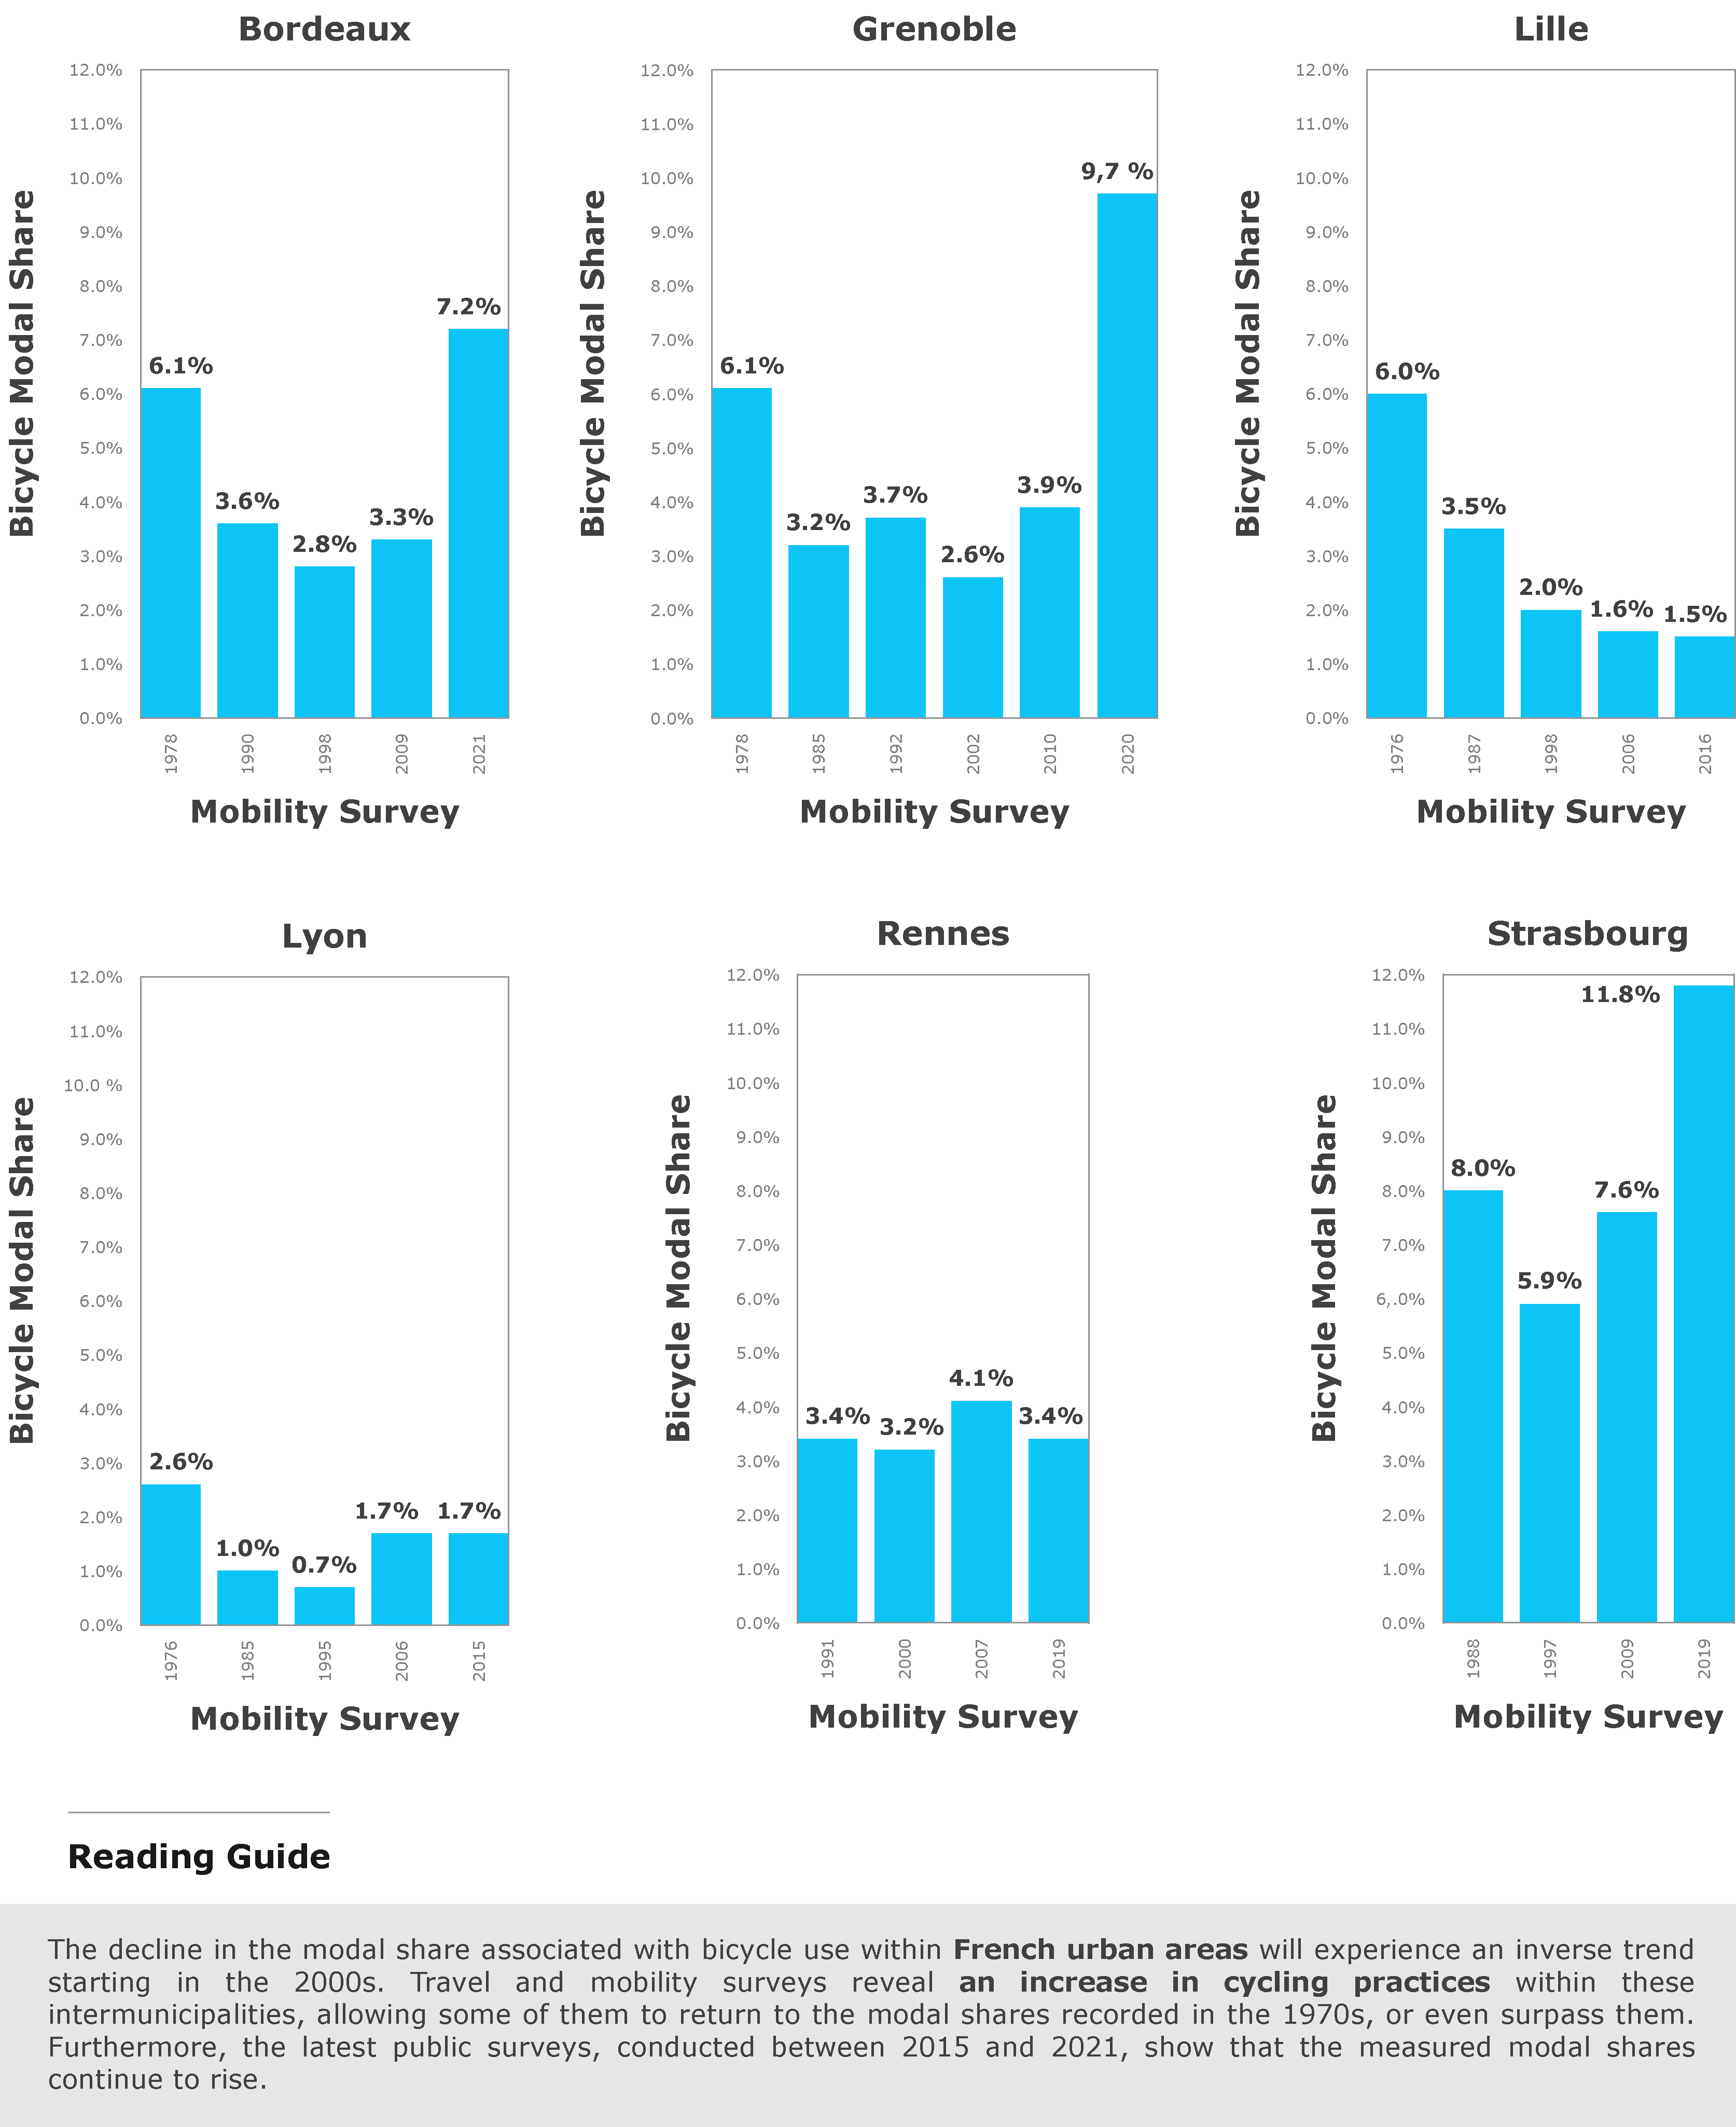
\includegraphics[width=1\columnwidth]{src/Figures/Chap-1/EN_Part_modale_velo_evolution.pdf}}
    \vspace{5pt}
    \begin{flushleft}\scriptsize{
    Note: the territories refer to their intermunicipal scale, while the mobility surveys relate to the \acrfull{EMD} corpus based on the \textsl{Certu} standard or certified by \textsl{Cerema}.
    }\end{flushleft}
    \begin{flushright}\scriptsize{
    Datasets: analysis from \textcolor{blue}{\textcite[48]{certu_usagers_2013}}\index{Certu@\textsl{Certu}|pagebf}\index{Cerema@\textsl{Cerema}|pagebf}\index{Jolly, Thomas|pagebf}
    \\
    Graphic adaptation and reinterpretation: \textcolor{blue}{Dylan Moinse (2025)}
    }\end{flushright}
\end{figure}

% Bicycle Resurgence in France
The \Commas{resurgence} of the bicycle in French territories \textcolor{blue}{\autocites[137-168]{heran_retour_2015}[44]{eskenazi_voir_2022}}\index{Héran, Frédéric|pagebf}\index{Eskenazi, Manon|pagebf} is part of a dynamic that began over forty years ago. This revival marks a second phase of conquest for the bicycle, long disqualified in daily mobility \textcolor{blue}{\autocite[26]{papon_retour_2012}}\index{Papon, Francis|pagebf}, while the utility use of the bicycle continues to decline in French cities, with a decrease of 50\% to 75\% between 1975 and 1990 \textcolor{blue}{\autocite[48]{certu_usagers_2013}}\index{Certu@\textsl{Certu}|pagebf}\index{Cerema@\textsl{Cerema}|pagebf}\index{Jolly, Thomas|pagebf}. Already in 1976, the newspaper \textsl{Le Monde} pointed out a contradiction in \Commas{mocking} the \Commas{forgotten} cyclists, while the bicycle fleet, estimated at 17 million, rivaled the number of private cars in possession \textcolor{blue}{\autocite{ambroise-rendu_creation_1976}}\index{Ambroise-Rendu, Marc|pagebf}\index{Le Monde@\textsl{Le Monde}|pagebf}. Mobility surveys conducted from the 2000s highlight a resurgence of the bicycle in daily mobility practices (see \hyperref[fig-chap1:evolution-part-modale-velo]{Figure~\ref{fig-chap1:evolution-part-modale-velo}}, page~\pageref{fig-chap1:evolution-part-modale-velo}). The Lyon metropolitan area saw the bicycle modal share quadruple between 1995 and 2006, while that of \acrfull{MEL} compensated for its decline between 1998 and 2006 \textcolor{blue}{\autocite[243]{dauncey_french_2012}}\index{Dauncey, Hugh|pagebf}. This phenomenon can be explained by growing environmental concerns, combined with the repercussions of successive economic and energy crises \textcolor{blue}{\autocite[138]{heran_retour_2015}}\index{Héran, Frédéric|pagebf}, as well as the densification of associative networks and changes in legal and regulatory frameworks \textcolor{blue}{\autocite[55]{sebban_complementarite_2003}}\index{Sebban, Annie-Claude|pagebf}\index{Motte, Alain|pagebf}. This period also saw the emergence of new types of bicycles, such as city bikes designed for urban use, or the aluminum folding bicycle \Marque{Brompton} \textcolor{blue}{\autocite[55]{sebban_complementarite_2003}}\index{Sebban, Annie-Claude|pagebf}\index{Motte, Alain|pagebf}. But it was especially the 1995 public transport strike, widely followed, that marked a decisive moment in this shift, allowing the bicycle to reposition itself as a credible alternative. The resurgence of the bicycle was accompanied by a sociological and spatial transformation: while the 1970s bicycle was mostly used by captive populations in suburban areas, the 1990s saw the emergence of users from middle and upper classes, moving within urban areas\footnote{~
    According to \textcolor{blue}{Frédéric} \textcolor{blue}{\textcite[143]{heran_retour_2015}}\index{Héran, Frédéric|pagebf}, \Commas{\textsl{In 1982, the typical cyclist was a rather young man, without a driver's license, from a large family, working-class or agricultural, often immigrant, with modest income and little or no motorized transport, living in the suburbs or a provincial town. He rode his bike to school or work, dreaming of buying a moped and, one day, a car. According to the results of the 2007-2008 ENTD, these users are still mostly men (63\%), but now mostly public service executives and professionals, much more rarely workers or employees.}}. Moreover, urban cyclists replaced the \Commas{proletarians of traffic} \textcolor{blue}{\autocite{ambroise-rendu_creation_1976}}\index{Ambroise-Rendu, Marc|pagebf}, becoming a French specificity due to investments almost exclusively focused on city centers \textcolor{blue}{\autocite[144]{heran_retour_2015}}\index{Héran, Frédéric|pagebf}.
} \textcolor{blue}{\autocite[143]{heran_retour_2015}}\index{Héran, Frédéric|pagebf}.%%Translated%%

% Transition
Although the bicycle's modal share remains modest in France—at 3\% of trips, compared to 10\% in Germany and 27\% in the Netherlands—this period is marked by an unprecedented momentum in favor of utility cycling \textcolor{blue}{\autocite[222]{dauncey_french_2012}}\index{Dauncey, Hugh|pagebf}. Local initiatives such as Strasbourg's \textsl{Plan vélo}, which transformed a fragmented cycling network into a continuous mesh of 483 km in 2006, illustrate this dynamic. Since the 2010s, the bicycle has become deeply linked to environmental and public health issues. In the face of urban pollution and car congestion, it is seen as an environmentally low-impact solution, beneficial for public and economic health. Efforts to promote its development reflect a desire to foster true \Commas{ecomobility} \textcolor{blue}{\autocites[4]{sebban_complementarite_2003}{heran_transition_2018}}\index{Sebban, Annie-Claude|pagebf}\index{Motte, Alain|pagebf}\index{Héran, Frédéric|pagebf}, marking a return of the \Commas{forgotten modes} to daily mobility practices \textcolor{blue}{\autocite[35]{papon_retour_2012}}\index{Papon, Francis|pagebf}. It would also have been possible to discuss the shared history of other \Commas{urban gliding objects}, such as the skateboard or roller skates\footnote{~
    This perspective differs somewhat for these other vehicles, which remain primarily associated with leisure and are not intended to meet needs for directive mobility or to share road space in a structured way.
}, but the goal here is not to provide an exhaustive analysis or to retrace the entire history of cycling. The intention is rather to connect the development of bicycles to the legacies of diffuse urban planning, shaped by the automobile. The investments made to bring the bicycle to the forefront have been accompanied by local initiatives, including the establishment of cycling infrastructure and the installation of mobility services, such as \acrshort{PBS} systems \textcolor{blue}{\autocite[244]{dauncey_french_2012}}\index{Dauncey, Hugh|pagebf}, as well as the deployment of electromobility.%%Translated%%

% 1.2.2.
\needspace{1\baselineskip} % Reserve space
\subsection{Expansion of the Offer through Electric Motorization and the Introduction of Shared Vehicle Systems
    \label{chap1:velo-micromobilite-innovations}
    }

    % Introduction
While the use of bicycles increased 32-fold between 1894 and 1934 \textcolor{blue}{\autocite[139]{orselli_usages_2008}}\index{Orselli, Jean|pagebf}, not without significant challenges in social acceptance, it later declined in favor of the automobile, which faced similar issues of appropriation. A neoliberal reading of urban dynamics clearly emerges through the rise of shared mobility services, first with stations, then without stations. These systems reflect a shift towards urban planning that is more entrepreneurial and a redefinition of the traditional roles of public authorities \textcolor{blue}{\autocites[169]{delaunay_mobilites_2017}{frotey_maxime_2017}}\index{Frotey, Julia|pagebf}\index{Delaunay, Teddy|pagebf}\index{Lesteven, Gaële|pagebf}. However, the debate truly crystallizes around the sharing of public space. These controversies recall historical struggles for the sharing of road space, already observed with the successive arrival of horse-drawn transportation, trams, and then automobiles. Each new mobility technology, by transforming uses and social relationships in urban space, reactivates conflictual dynamics related to cohabitation and the distribution of spatial resources\footnote{~
    We can also mention the disputes arising from the development of the tramway during its golden age, from the late 19\textsuperscript{th} century to the interwar period \textcolor{blue}{\autocite[281]{flonneau_concurrence_2007}}\index{Flonneau, Mathieu|pagebf}. These controversies resurfaced during its gradual return in the 2000s, accompanied by both popular and political concerns. Indeed, the tramway was perceived as an outdated means of transport from another era \textcolor{blue}{\autocite[110]{gardon__2014}}\index{Flonneau, Mathieu|pagebf}. However, these negative representations faded in favor of a renewed and modern image, thanks to the integration of technical innovations such as low and ultra-low floors, as well as ground-based power supply systems. This tramway revival, far from being a consensual process, nevertheless generated tensions, especially with the automobile, which it directly competes with. The resulting power dynamics led to the reconfiguration of tramway project routes, often designed to minimize impacts on road space and parking areas for cars. In some cases, this spatial reconciliation led to the construction of underground tramway sections, thus preserving car lanes \textcolor{blue}{\autocite[10]{richer_tramways_2012}}\index{Richer, Cyprien|pagebf}\index{Hasiak, Sophie|pagebf}. Furthermore, the tramway was also accused of competing with other pre-existing public transport systems, notably regional rail networks \textcolor{blue}{\autocite[36]{cete_nord_picardie_evaluer_2013}}.
}. However, the \Commas{return} of the bicycle to urban areas in recent decades has been accompanied by the emergence of new categories of cycles. This diversification of the offer in \Commas{alternative mobility} \textcolor{blue}{\autocite[91-92]{vincent-geslin__2012}}\index{Vincent-Geslin, Stéphanie|pagebf} is marked by the rise of electromobility, initially illustrated by the redeployment of \acrshort{e-Bike}, followed by the development of \acrshort{PeS}, as well as new acquisition models such as the provision of shared fleets of bicycles and scooters. As we have observed, these vehicles undergo cycles of innovation, whether technical, service-based, or organizational. By adopting a historical perspective on the evolution of the role these vehicles play, it becomes clear that, despite being perceived as outdated or limited to children's leisure use, a century of innovations applied to these objects has allowed their reintroduction in modernized forms, in an opportune context. By combining nostalgia and modernity, these vehicles have gradually asserted themselves as reliable modes of transport, benefiting from both electrification, which extends their ease and range of use, and sharing systems, which increase their accessibility and visibility in public space. This phenomenon can be interpreted through the notion of \Commas{retro-innovation}, from the field of \textsl{marketing} and communication, defined as the reinvention of a product or activity area through technological innovations, aimed at granting it a new use while establishing a connection with the past \textcolor{blue}{\autocite{barthelot_retro-innovation_2018}}\index{Barthelot, Bertrand|pagebf}. Among the three categories constituting retro-innovation, electrified cycles and shared systems fit into the trend known as \textsl{inn-old-vation}, which involves integrating technological innovations to adapt a product to pre-existing needs \textcolor{blue}{\autocite{lamy_retro-innovation_2016}}\index{Lamy, Alexia|pagebf}. However, as we will see, the major challenge lies in introducing these innovations, whether technical or social, a challenge that has accompanied the bicycle since the early days of its modern history \textcolor{blue}{\autocite[33]{jouenne_quest-ce_2022}}\index{Jouenne, Noël|pagebf}.%%Translated%%

% 1.2.2.1.
\needspace{1\baselineskip} % Reserve space
\subsubsection*{Contribution of Electromobility to the Diversification of Bicycles and Micromobility
    \label{chap1:velo-micromobilite-innovations-electromobilite}
    }

    % Introduction
Alongside the development of bicycles and folding bicycles, new electric propulsion modes of transport have emerged, expanding the family of cycles \textcolor{blue}{\autocite[5]{lopez-escolano_mobilites_2019}}\index{López-Escolano, Carlos|pagebf}\index{Campos, Ángel Pueyo|pagebf}. These include the \acrfull{e-Bike}, whether folding or not, the \acrfull{PeS}, as well as a variety of mobility devices grouped under the term \Commas{micromobility} (see \hyperref[fig-chap1:ecosysteme-micromobilite]{Figure~\ref{fig-chap1:ecosysteme-micromobilite}}, page~\pageref{fig-chap1:ecosysteme-micromobilite}), such as the monowheel (or gyroroue), the hoverboard, and the segway. The list of \acrfull{NIEV} continues to grow, illustrating a modal diversification made possible notably by the reduction in manufacturing costs, the miniaturization of components, and the increased efficiency of electric batteries, which make them more portable\footnote{~
    The 1990s marked a turning point for \textsl{pedelecs}, when several technical advancements converged to increase their practicality and appeal. The introduction and commercialization of lighter and more efficient batteries, such as the \acrfull{NiCd} battery and, later, the \acrfull{NiMH} battery, played a strategic role in their evolution. These new batteries offer a much better energy-to-weight ratio than their predecessors, making electric bicycles both lighter, more maneuverable, and with better range. The introduction of the \acrfull{Li-ion} accumulator, compared to previous batteries, marked another milestone. This type of battery, of equivalent size, offers 32\% more energy capacity and a 25\% reduction in weight. Moreover, the \acrshort{Li-ion} battery has high current discharge, no memory effect, and the ability to recharge the battery at any time.
} \textcolor{blue}{\autocites[430]{bertoluzzo_development_2011}[2]{schultz_micromobility_2019}[430]{pages_nouveaux_2021}}\index{Schultz, Stéphane|pagebf}\index{Grisot, Sylvain|pagebf}\index{Bertoluzzo, Manuele|pagebf}\index{Buja, Giuseppe|pagebf}\index{Pages, Thibaud|pagebf}\index{Lammoglia, Adrien|pagebf}\index{Josselin, Didier|pagebf}.%%Translated%%

% Figure Ecosystem of Bicycles and Micromobility
\begin{figure}[h!]\vspace*{4pt}
        \caption{Ecosystem of \Commas{individual and local mobility}, human-powered, assisted, or motorized.}
        \label{fig-chap1:ecosysteme-micromobilite}
        \centerline{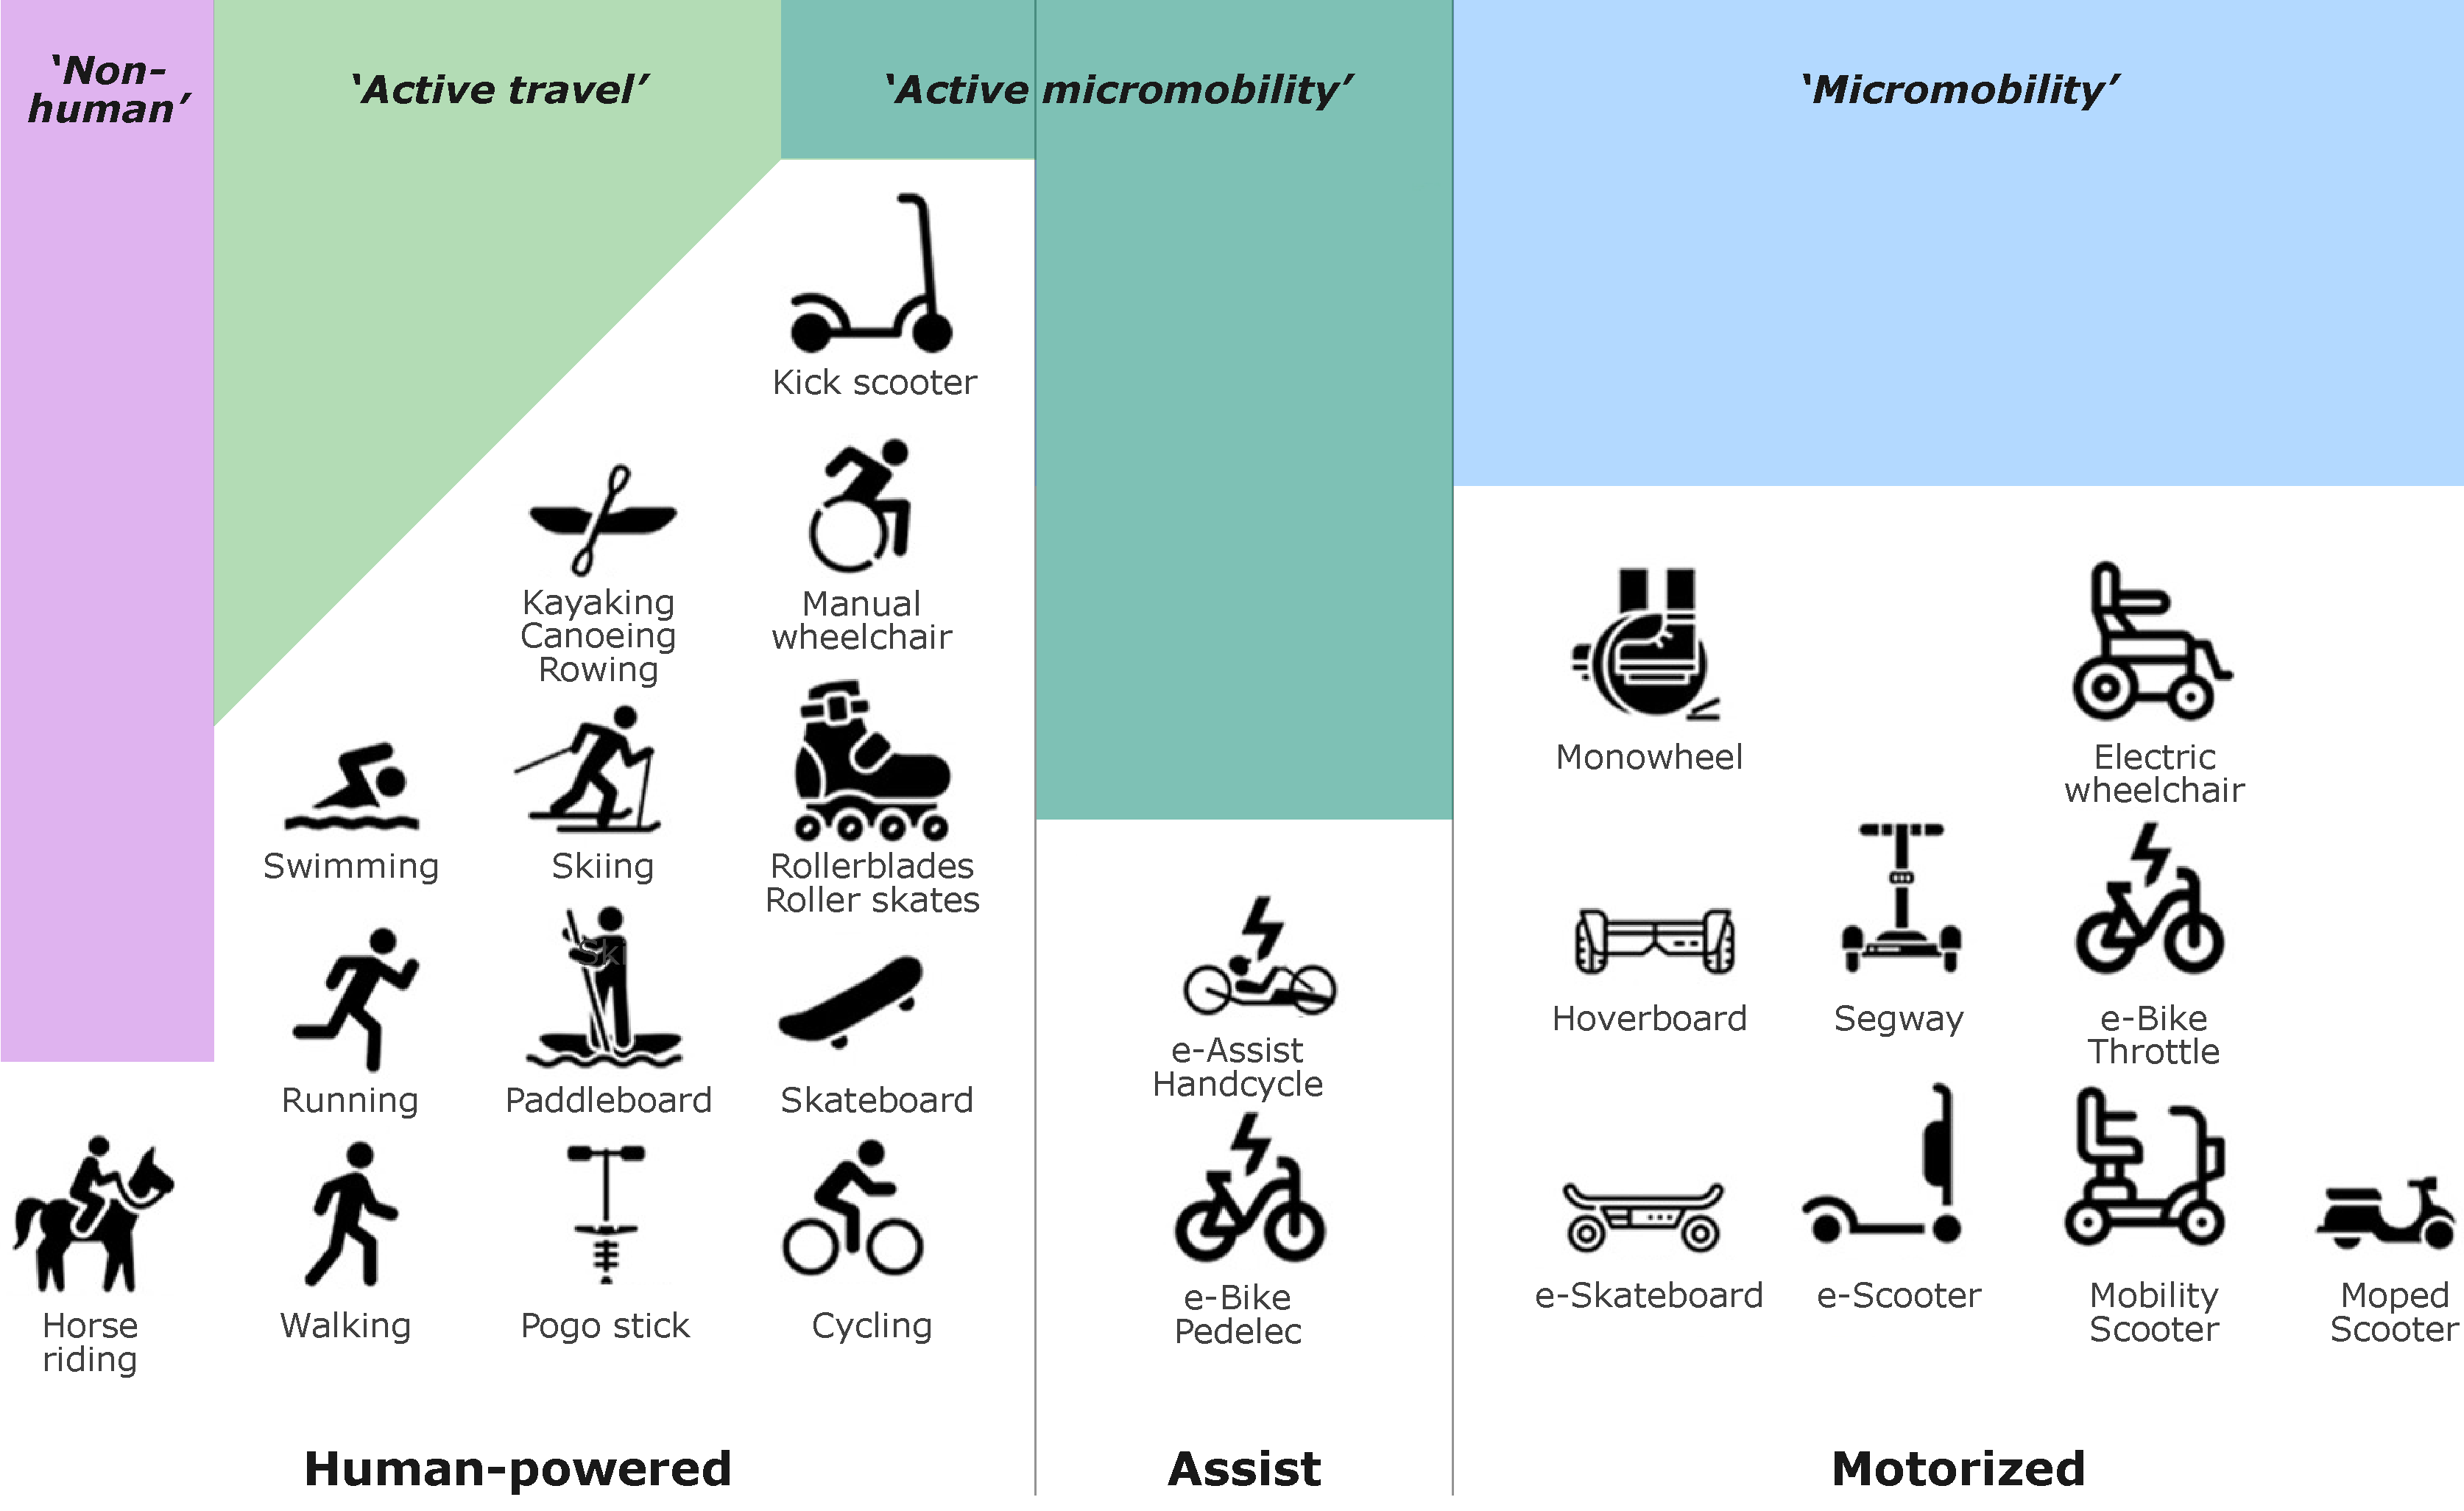
\includegraphics[width=1\columnwidth]{src/Figures/Chap-1/EN_Ecosysteme_micromobilite.pdf}}
        \vspace{5pt}
        \begin{flushright}\scriptsize{
        Source: \textcolor{blue}{\textcite[155]{cook_more_2022}}\index{Cook, Simon|pagebf}\index{Stevenson, Lorna|pagebf}\index{Aldred, Rachel|pagebf}\index{Kendall, Matt|pagebf}\index{Cohen, Tom|pagebf}
        \\
        Graphic adaptation: \textcolor{blue}{Dylan Moinse (2024)}
        }\end{flushright}
    \end{figure}

    % Contemporary History of e-Bike
In 1993, the Japanese motorcycle manufacturer \Marque{Yamaha Motor Company} introduced the first commercially successful electric bicycle, featuring a pedal-assist function (\textsl{Power Assist System}) and powered by a removable \acrshort{NiMH} battery \textcolor{blue}{\autocite[430]{bertoluzzo_development_2011}}\index{Bertoluzzo, Manuele|pagebf}\index{Buja, Giuseppe|pagebf}. This bicycle offers notable advantages over the traditional lead-acid battery, providing a lighter battery, less sensitive to ambient temperature variations, and with a longer lifespan. The pedal-assist system not only extended the battery's life but also made the user experience more intuitive. Because of these qualities, \textcolor{blue}{Noël} \textcolor{blue}{\textcite[25]{jouenne_quest-ce_2022}}\index{Jouenne, Noël|pagebf} describes the \acrshort{e-Bike} as an \Commas{electromechanical assisted bicycle} in his \acrfull{HDR} on the ethnology of the bicycle as a technical and social object, emphasizing the energy mix required for movement. From 2003, the electric bicycle benefited from the development and commercialization of \acrshort{Li-ion} batteries \textcolor{blue}{\autocite[6]{hung_review_2020}}\index{Hung, Nguyen Ba|pagebf}\index{Lim, Ocktaeck|pagebf}. In France, \acrshort{e-Bike} sales experienced spectacular growth, rising from 37,000 units sold in 2011 to 338,000 in 2018, reaching 738,000 in 2022, before a slight decrease to 671,000 products in 2023. These figures represent 43\% of total electric vehicle sales in 2023 \textcolor{blue}{\autocite{union_sport__cycle_chiffres_2024}}\index{Union Sport \& Cycle@\textsl{Union Sport \& Cycle}|pagebf}. Alongside \acrshort{e-Bike}, new forms of bicycles such as cargo bikes and tricycles have expanded the possibilities of electric bicycle use. These models facilitate not only long-distance travel or use by elderly or mobility-impaired individuals but also the transport of people and heavy goods. They thus open new perspectives for family travel, bike-taxi services, urban logistics, and self-employment. According to \textcolor{blue}{\textcite[24]{mason_global_2015}}\index{Mason, Jacob|pagebf}\index{Fulton, Lew|pagebf}\index{McDonald, Zane|pagebf}, the modal share of bicycles, stimulated by the growing popularity of \acrshort{e-Bike}, could reach 17\% by 2030 and 22\% by 2050 among OECD countries.%%Translated%%

% Contemporary History of TEP + Transition
Alongside the rise of the \acrshort{e-Bike}, the scooter makes a return to the forefront, first as a toy, and then gradually adopted by teenagers\footnote{~
    The spread of the modern scooter was facilitated by a major technical innovation that made it lighter, more durable, and more maneuverable thanks to the use of aluminum, a material that also made it foldable \textcolor{blue}{\autocite{arte_histoire_2014}}. In 1996, Swiss businessman \textcolor{blue}{Wim Ouboter} played a pivotal role in the evolution of the scooter. He founded his own company, \Marque{Micro Mobility Systems}, and by 1999, designed \Commas{micro-scooters}, combining the aesthetics of the scooter with wheels inspired by the \textsl{skateboard} \textcolor{blue}{\autocite{les_numeriques_futur_2015}}\index{Les Numériques@\textsl{Les Numériques}|pagebf}. Quickly, this model, marketed under the \Marque{Razor} brand, became a global phenomenon, reaching one million units sold in 2000 before the excitement waned. Despite this decline, the scooter maintained its status as a toy primarily intended for children. In the United States, it \Commas{invaded the cul-de-sacs of residential areas}, and the \textsl{Toy Association} named this model \Commas{Toy of the Year} in 2000 \textcolor{blue}{\autocite{bloomberg_citylab_man_2018}}. However, this enthusiasm quickly faded \textcolor{blue}{\autocite[25]{university_of_st_gallen_micro_2011}}\index{University of St. Gallen@\textsl{University of St. Gallen}|pagebf}. At the same time, the scooter evolved, being redeployed in a different context. A change in usage and customer base occurred: the reinforced scooter became a tool for a new sport, freestyle, inspired by BMX (\textsl{bicycle motocross}) and \textsl{skateboarding}. This sport, which involves performing acrobatic stunts (\textsl{tricks}), attracted a new generation of users, the \textsl{trottiriders} \textcolor{blue}{\autocite{micro-mobility_innovations_2018}}\index{Micro-mobility@\textsl{Micro-mobility}|pagebf}. Thus, the scooter gradually ceased to be seen as a mere toy and became a popular piece of equipment among teenagers and young adults, drawn to extreme sports and urban culture \textcolor{blue}{\autocite{ma_trott_histoire_2020}}.
} before undergoing a transformation through a modernized design and the integration of an electric battery. The man considered the \Commas{pioneer of the scooter revolution}, \textcolor{blue}{Wim Ouboter}, initiated this transformation based on his personal experience\footnote{~
    \textcolor{blue}{Wim Ouboter} relates that his interest in the scooter stemmed from his personal experience. As a child, he and his sister used old scooters, the latter being unable to ride a bicycle or ski due to a physical disability. However, it was at the age of 30 that the true revelation occurred. According to his account, the Swiss entrepreneur realized that his favorite sausage restaurant, located in Zurich, was too far to walk but not far enough to justify using a bike or car \textcolor{blue}{\autocite{ma_trott_histoire_2020}}.
} \textcolor{blue}{\autocite{ma_trott_histoire_2020}}\index{Ma Trott'@\textsl{Ma Trott'}|pagebf}. The scooter was rehabilitated with the creation of \Marque{Micro}, designed for what are termed \Commas{micro-distances}, situated between trips that are too long to walk and too short to use a car or a bike \textcolor{blue}{\autocite{oconnell_travel_2002}}\index{O'Connel, Dee|pagebf}. In line with the electrification of urban mobility in 2003, the Swiss entrepreneur expanded his range by developing electric models, still targeting an adult clientele \textcolor{blue}{\autocite{ma_trott_histoire_2020}}\index{Ma Trott'@\textsl{Ma Trott'}|pagebf}. But it was truly the launch of the \Marque{Xiaomi Mi Electric Scooter} (M365) in 2016, first in China, that disrupted the market. Released in Europe in 2018, the \acrshort{PeS} became a global success thanks to its affordable price and ergonomic design. Massively adopted for personal use, it also became a benchmark model for a multitude of shared scooter fleets. In France, the popularity of the \acrshort{PeS} was immediate: according to the barometer of the \acrfull{FP2M}, sales started at 233,000 units in 2018, rose to 478,800 units the following year, and reached 678,000 units in 2023 \textcolor{blue}{\autocites[1]{fp2m_barometre_2021}[1]{fp2m_ventes_2023}}\index{FP2M@\textsl{FP2M}|pagebf}. These numbers now surpass \acrshort{e-Bike} sales, which are also expanding. The example of the scooter, whether human-powered or electric, and that of the \acrshort{e-Bike}, folding or standard, perfectly illustrate the diversification of mobility modes in urban areas, both in forms accessible for purchase and rental.%%Translated%%

% 1.2.2.2.
\needspace{1\baselineskip} % Reserve space
\subsubsection*{The Sharing Economy in Service of Shared Mobility
    \label{chap1:velo-micromobilite-innovations-partage}
    }

    % Self-service with station - History 1
The genesis of \acrshort{PBS} lies within the history of social movements that led to the return of bicycles to cities \textcolor{blue}{\autocite[23]{hure_mobilites_2019}}\index{Huré, Maxime|pagebf}. The idea of a \Commas{smart bike} shared in public space, accessible to all without the need for personal acquisition, first found its applications in 1965 thanks to a Dutch anarchist collective, \textsl{Provo}. As part of their fifth \Commas{provocation} (\textsl{Witte Fietsenplan}) and ahead of the 1966 municipal elections, this protest and libertarian movement made available to the citizens of Amsterdam about fifty white-painted bicycles, freely placed on the streets, with the goal of freeing the city from urban congestion\footnote{~
    The \textsl{Provo} group advocated for a municipal initiative to provide the population with 10,000 free bicycles, self-managed by a participatory system. In protest against the municipality's refusal of their project, the collective included a list of voters and relaunched about a hundred abandoned bicycles, repairing and painting them white \textcolor{blue}{\autocite[29]{hure_mobilites_2019}}\index{Huré, Maxime|pagebf}.
} \textcolor{blue}{\autocites[6]{smart_provo_2012}{demain_la_ville_doit-velib_2018}}\index{Smart, Alan|pagebf}\index{Demain La Ville@\textsl{Demain La Ville}|pagebf}. Although pioneering, this form of action remained illegal according to public authorities, yet it gave rise to the first generation of \acrshort{PBS}, based on a free system \textcolor{blue}{\autocite[160]{shaheen_bikesharing_2010}}\index{Shaheen, Susan~A.|pagebf}\index{Guzman, Stacey|pagebf}\index{Zhang, Hua|pagebf}. La Rochelle is often recognized as the first city to institutionalize such a system in 1976 with its \textsl{municipal bicycles}, also called \textsl{Yellow Bikes}, a fleet of 350 bikes spread over three rental points\footnote{~
    The very visible experience of the municipal system in La Rochelle raises the question of the transformations in public urban action regarding mobility, previously heavily dependent on state services, shifting from state dirigisme to a regulatory state that remains the primary funder of this project. With its 300 \acrshort{PBS}, the mayor at the time, \textcolor{blue}{Michel Crépeau}, aimed to \Commas{normalize} the use of bicycles in the city. This policy set up a restricted access area, limited to the interior of the old fortress, and hours, from 8 a.m. to 8 p.m., with system regulation dependent on citizen participation \textcolor{blue}{\autocite[31]{hure_mobilites_2019}}\index{Huré, Maxime|pagebf}. Such a project, inaugurated six months before the municipal elections, allowed the mayor to build international recognition and legitimize a new urban policy for the rehabilitation of the city center, already constructing an early form of political and territorial marketing through these mobility services \textcolor{blue}{\autocite[31]{hure_mobilites_2019}}\index{Huré, Maxime|pagebf}. The following year, a second fleet of 100 free \acrshort{PBS} was established, funded through private sponsorship based on an advertising model. This initiative marked a turning point, as the use of advertising gradually became a central mode of financing for \acrshort{PBS} systems \textcolor{blue}{\autocite[32-35]{fleury_mobilites_2022}}\index{Huré, Maxime|pagebf}\index{Fleury, Antoine|pagebf}\index{Frétigny, Jean-Baptiste|pagebf}\index{Kanellopoulou, Dimitra|pagebf}.
}. This model inspired other initiatives, such as the one launched in Cambridge in 1993, and helped stabilize the commercial architecture of shared mobility as it is practiced today. Finally, the mechanisms and symbolic values of \acrshort{PBS} are largely inspired by those of the supermarket cart, as noted by \textcolor{blue}{Maxime} \textcolor{blue}{Maxime} \textcolor{blue}{\textcite[40]{hure_mobilites_2019}}\index{Huré, Maxime|pagebf}. Copenhagen marked a decisive step between 1989 and 1995 with the introduction of \textsl{Bycyklen}, a system utilizing the coin-deposit mechanism and bike stands. This system, considered the second generation of \acrshort{PBS}, was adopted in Europe and the United States, but problems of theft related to user anonymity persisted\footnote{~
    A notable alternative to the classic \acrshort{PBS} model is represented by the \textsl{Call a Bike} service, deployed in several German cities, starting with Munich in 2000. This system operates on a different principle: the bike, locked in the public space with a lock, can be borrowed and returned freely. Access to the bike requires contacting a dedicated service, allowing users to obtain the lock code for a fee. This system offers two modes of operation: \textsl{Call a Bike FLEX}, without stations, and \textsl{Call a bike FIX}, with stations \textcolor{blue}{\autocite[18]{6t-bureau_de_recherche_etude_2018}}. At the time, \textsl{Deutsche Bahn} considered deploying this system in about a hundred stations on the Intercités express network to promote intermodality.
} \textcolor{blue}{\autocite[160]{shaheen_bikesharing_2010}}\index{Shaheen, Susan~A.|pagebf}\index{Guzman, Stacey|pagebf}\index{Zhang, Hua|pagebf}. The third generation, embodied by the \textsl{Vélo à la carte} of Rennes in 1998, introduced identification and reservation technologies. This computerized system relies on kiosks, personal cards, and later mobile phones, enabling a \textsl{check-in} and \textsl{check-out} of the bike \textcolor{blue}{\autocite[8]{nlc_micromobility_2019}}\index{NLC@\textsl{NLC}|pagebf}.%%Translated%%

% Figure VLS map France
\begin{carte}[h!]\vspace*{4pt}
    \caption{Location and evolution of station-based bike-sharing services in France, in 2018.}
    \label{fig-chap1:carte-vls-france}
    \centerline{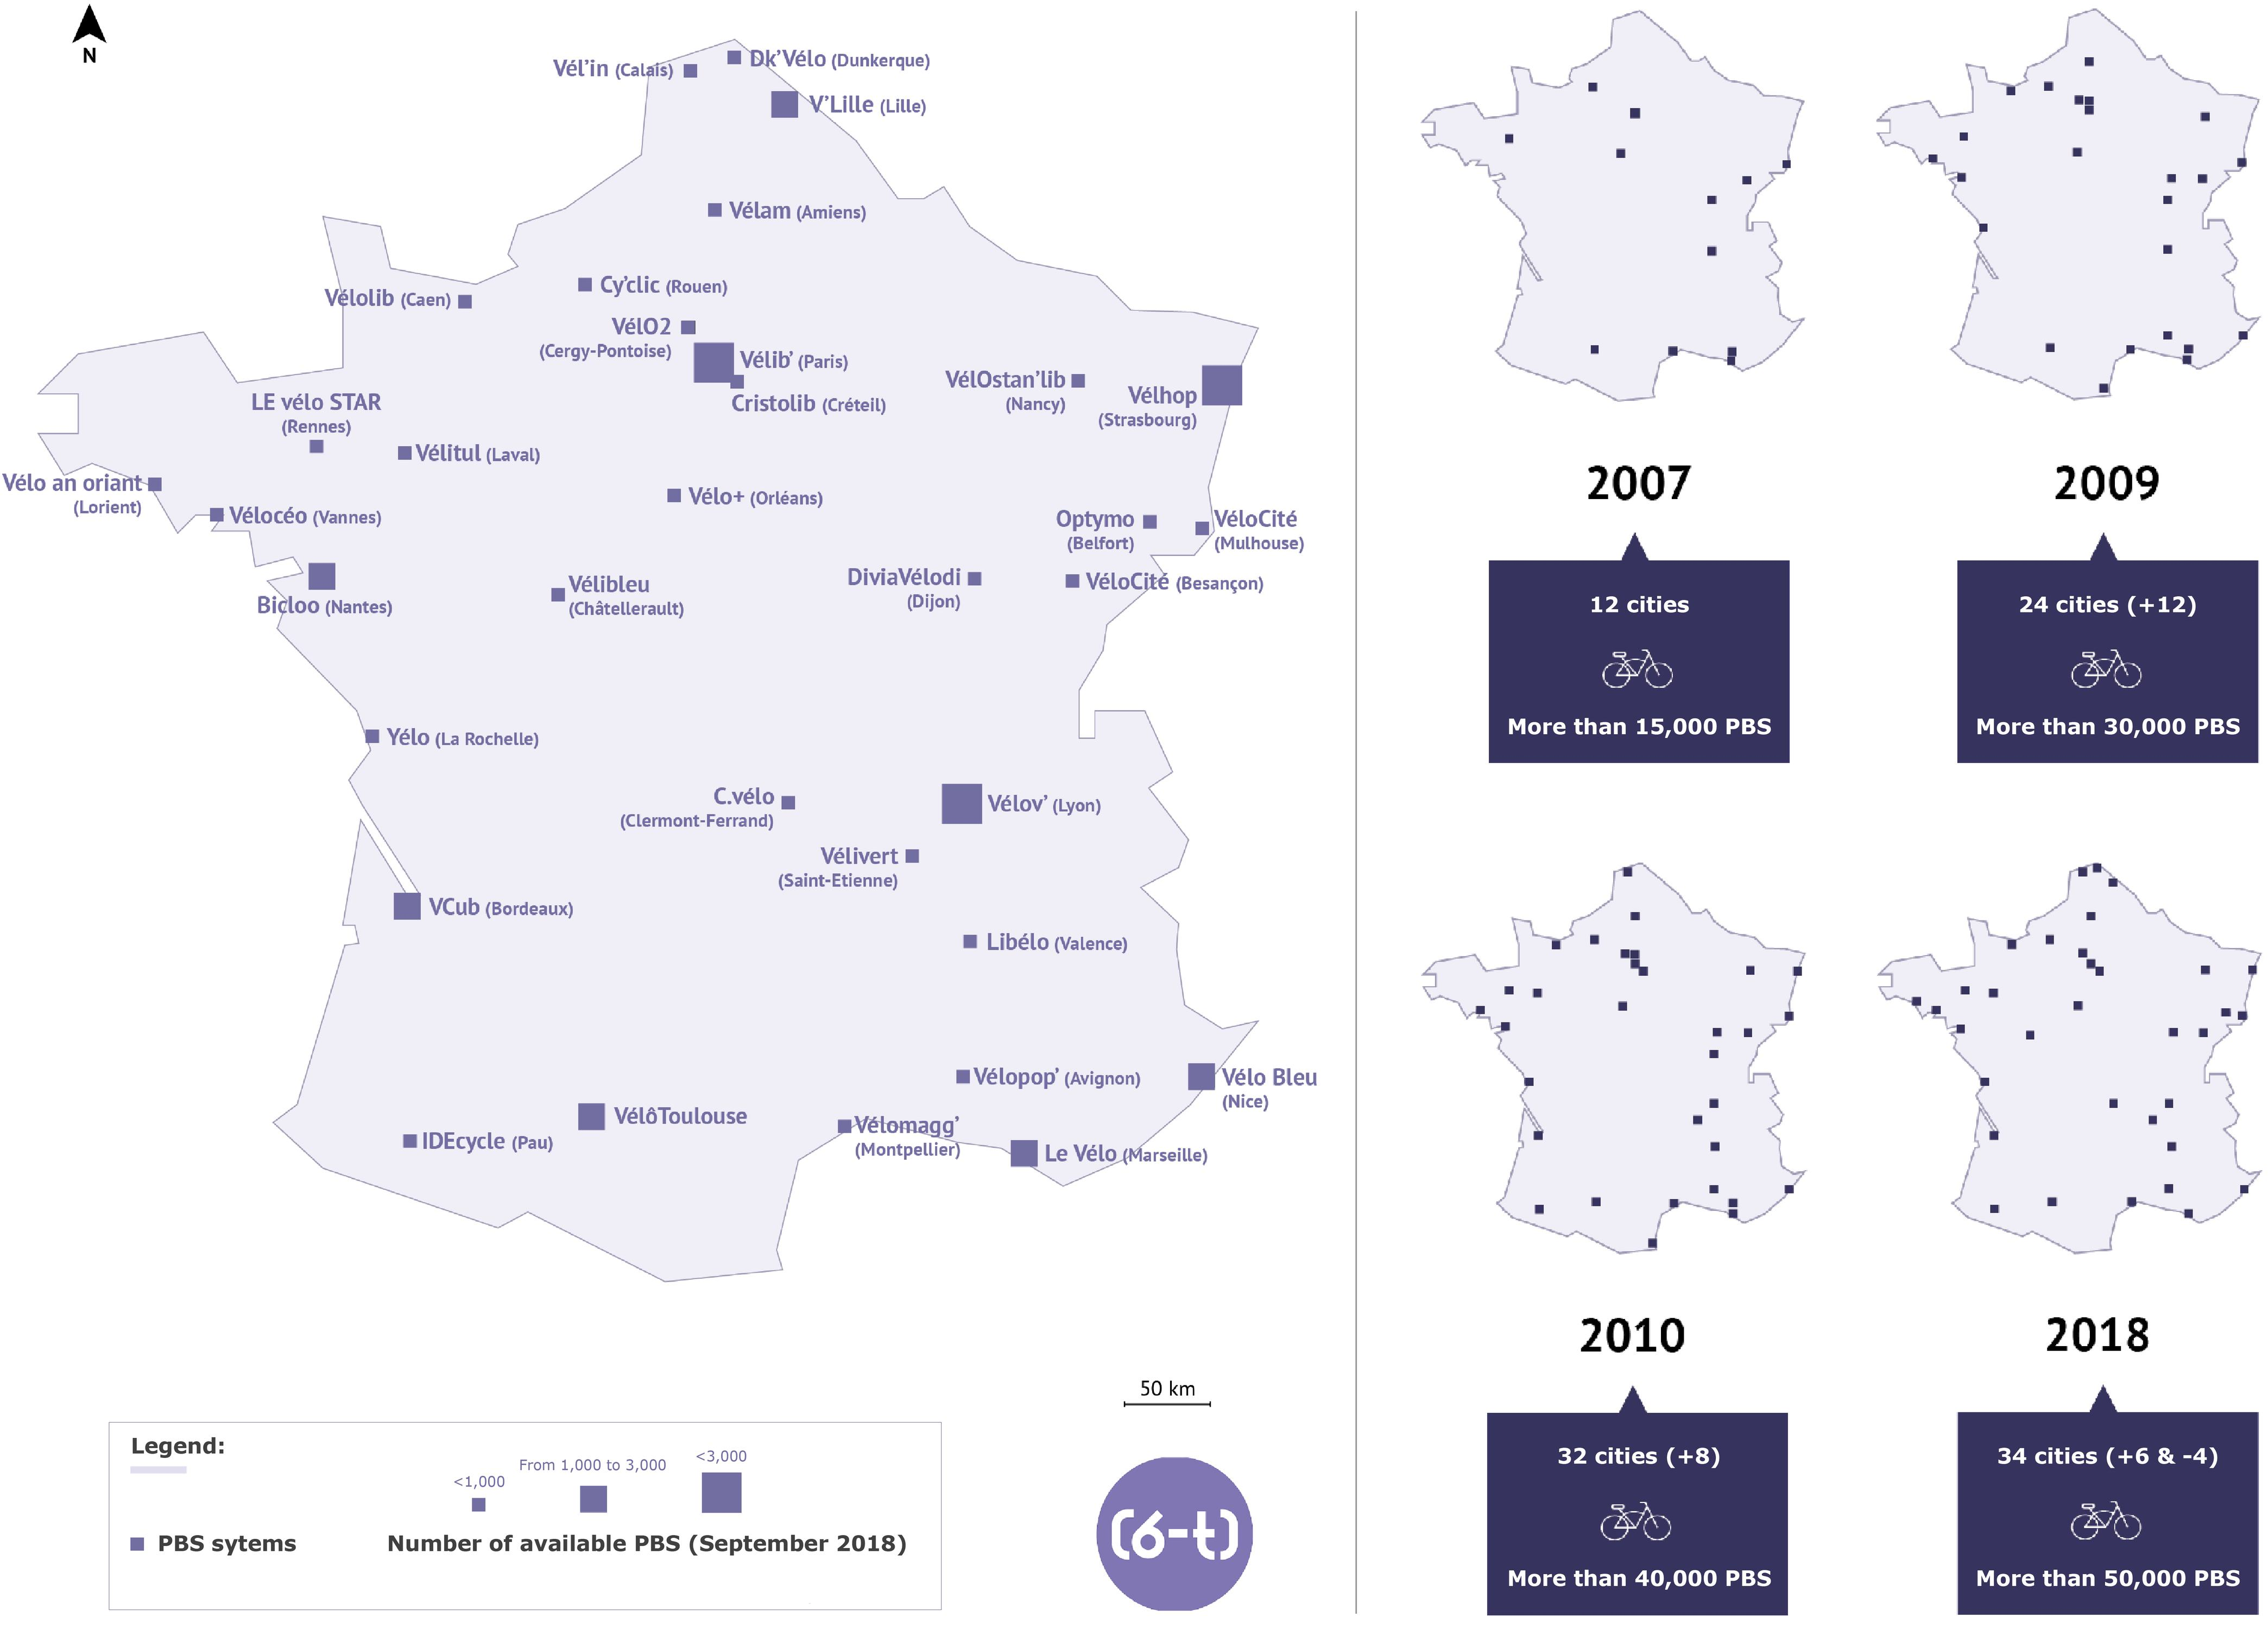
\includegraphics[width=1\columnwidth]{src/Figures/Chap-1/EN_Carte_VLS_France.jpg}}
    \vspace{5pt}
    \begin{flushright}\scriptsize{
    Source: \textcolor{blue}{\textcite{6t-bureau_de_recherche_lechappee_2018}}\index{Bureau de recherche 6t@\textsl{Bureau de recherche 6t}|pagebf}
    }\end{flushright}
\end{carte}

% Self-service with station - History 2
These innovations, combined with a pricing model based on time intervals, have become the international standard for \acrshort{PBS} systems \textcolor{blue}{\autocite[162]{shaheen_bikesharing_2010}}\index{Shaheen, Susan~A.|pagebf}\index{Guzman, Stacey|pagebf}\index{Zhang, Hua|pagebf}. However, it is Lyon, with \textsl{Vélo'v} in 2005, and Paris, with \textsl{Vélib'} in 2007, that popularized this model worldwide. These services became the benchmarks for \acrshort{PBS}, enabling France to take the lead in this area: by 2010, the country had 24 \acrshort{PBS} systems, with a total fleet of 36,000 bikes and 3,000 stations \textcolor{blue}{\autocite[161]{shaheen_bikesharing_2010}}\index{Shaheen, Susan~A.|pagebf}\index{Guzman, Stacey|pagebf}\index{Zhang, Hua|pagebf}, reaching 34 urban areas by 2018 (see \hyperref[fig-chap1:carte-vls-france]{Map~\ref{fig-chap1:carte-vls-france}}, page~\pageref{fig-chap1:carte-vls-france}). It is at the turn of this decade that the experiences of \acrshort{PBS} systems began to reveal a dominant management model: the \acrfull{PPP} \textcolor{blue}{\autocite[5]{hure_entre_2014}}\index{Huré, Maxime|pagebf}. More recently, a fourth generation has emerged, integrating \acrshort{e-Bike} for self-service, optimized locking mechanisms, touch interfaces, and interconnection with public transport systems \textcolor{blue}{\autocite[162]{shaheen_bikesharing_2010}}\index{Shaheen, Susan~A.|pagebf}\index{Guzman, Stacey|pagebf}\index{Zhang, Hua|pagebf}. It should be noted that while these initiatives are mostly the result of local or intercommunal projects led primarily by the largest urban areas \textcolor{blue}{\autocites[18]{fishman_bike_2013}[6]{ricci_bike_2015}}\index{Fishman, Elliot|pagebf}\index{Washington, Simon|pagebf}\index{Haworth, Narelle|pagebf}\index{Ricci, Miriam|pagebf}, their deployment remains marginal at the regional or national level\footnote{~
    Among these exceptions, we cannot avoid mentioning the Dutch system \textsl{OV-fiets}, literally translated as \textsl{public transport bikes}, integrated into the national railway network. Created in 2004 by an association, this \acrshort{PBS} system was taken over, starting in 2008, by the Dutch national railway company, \acrfull{NS} \textcolor{blue}{\autocites[151]{ploeger_sociotechnical_2020}[157]{waes_why_2020}}\index{Ploeger, Jan|pagebf}\index{Oldenziel, Ruth|pagebf}\index{Waes, Arnoud van|pagebf}\index{Farla, Jacco|pagebf}\index{Raven, Rob|pagebf}. Today, this mobility service covers 300 stations located near train stations and metro stops, with a fleet of 22,000 bikes. Its specificity lies in the fact that the rental occurs on a daily basis and requires that the bike be returned to the same station where it was borrowed \textcolor{blue}{\autocite[9]{ploeger_sociotechnical_2020}}\index{Caletrío, Javier|pagebf}, following a loop model, \textsl{2-way} type \textcolor{blue}{\autocite[13]{mangeart_vehicules_2022}}\index{Mangeart, Timothée|pagebf}\index{Bouteuil, Virginie|pagebf}.
} \textcolor{blue}{\autocite[225]{dauncey_french_2012}}\index{Dauncey, Hugh|pagebf}. In August 2022, according to the platform \textsl{The Meddin Bike-sharing World Map}\footnote{~
    \url{https://bikesharingworldmap.com}
}, which records and updates all shared mobility systems worldwide, 1,212 urban areas have \acrshort{PBS} services \textcolor{blue}{\autocite[7]{the_meddin_bike-sharing_world_map_meddin_2022}}\index{The Meddin Bike-sharing World Map@\textsl{The Meddin Bike-sharing World Map}|pagebf}, with the largest ones all located in China (see \hyperref[fig-chap1:carte-vls-monde]{Map~\ref{fig-chap1:carte-vls-monde}}, page~\pageref{fig-chap1:carte-vls-monde}). In addition to these, 80 so-called \Commas{hybrid} systems have emerged, combining a fleet of \acrshort{PBS} and a fleet of \acrfull{DBS}.%%Translated%%

% Figure VLS world map
\begin{carte}[h!]\vspace*{4pt}
    \caption{Location of major station-based bike-sharing services worldwide, in 2021.}
    \label{fig-chap1:carte-vls-monde}
    \centerline{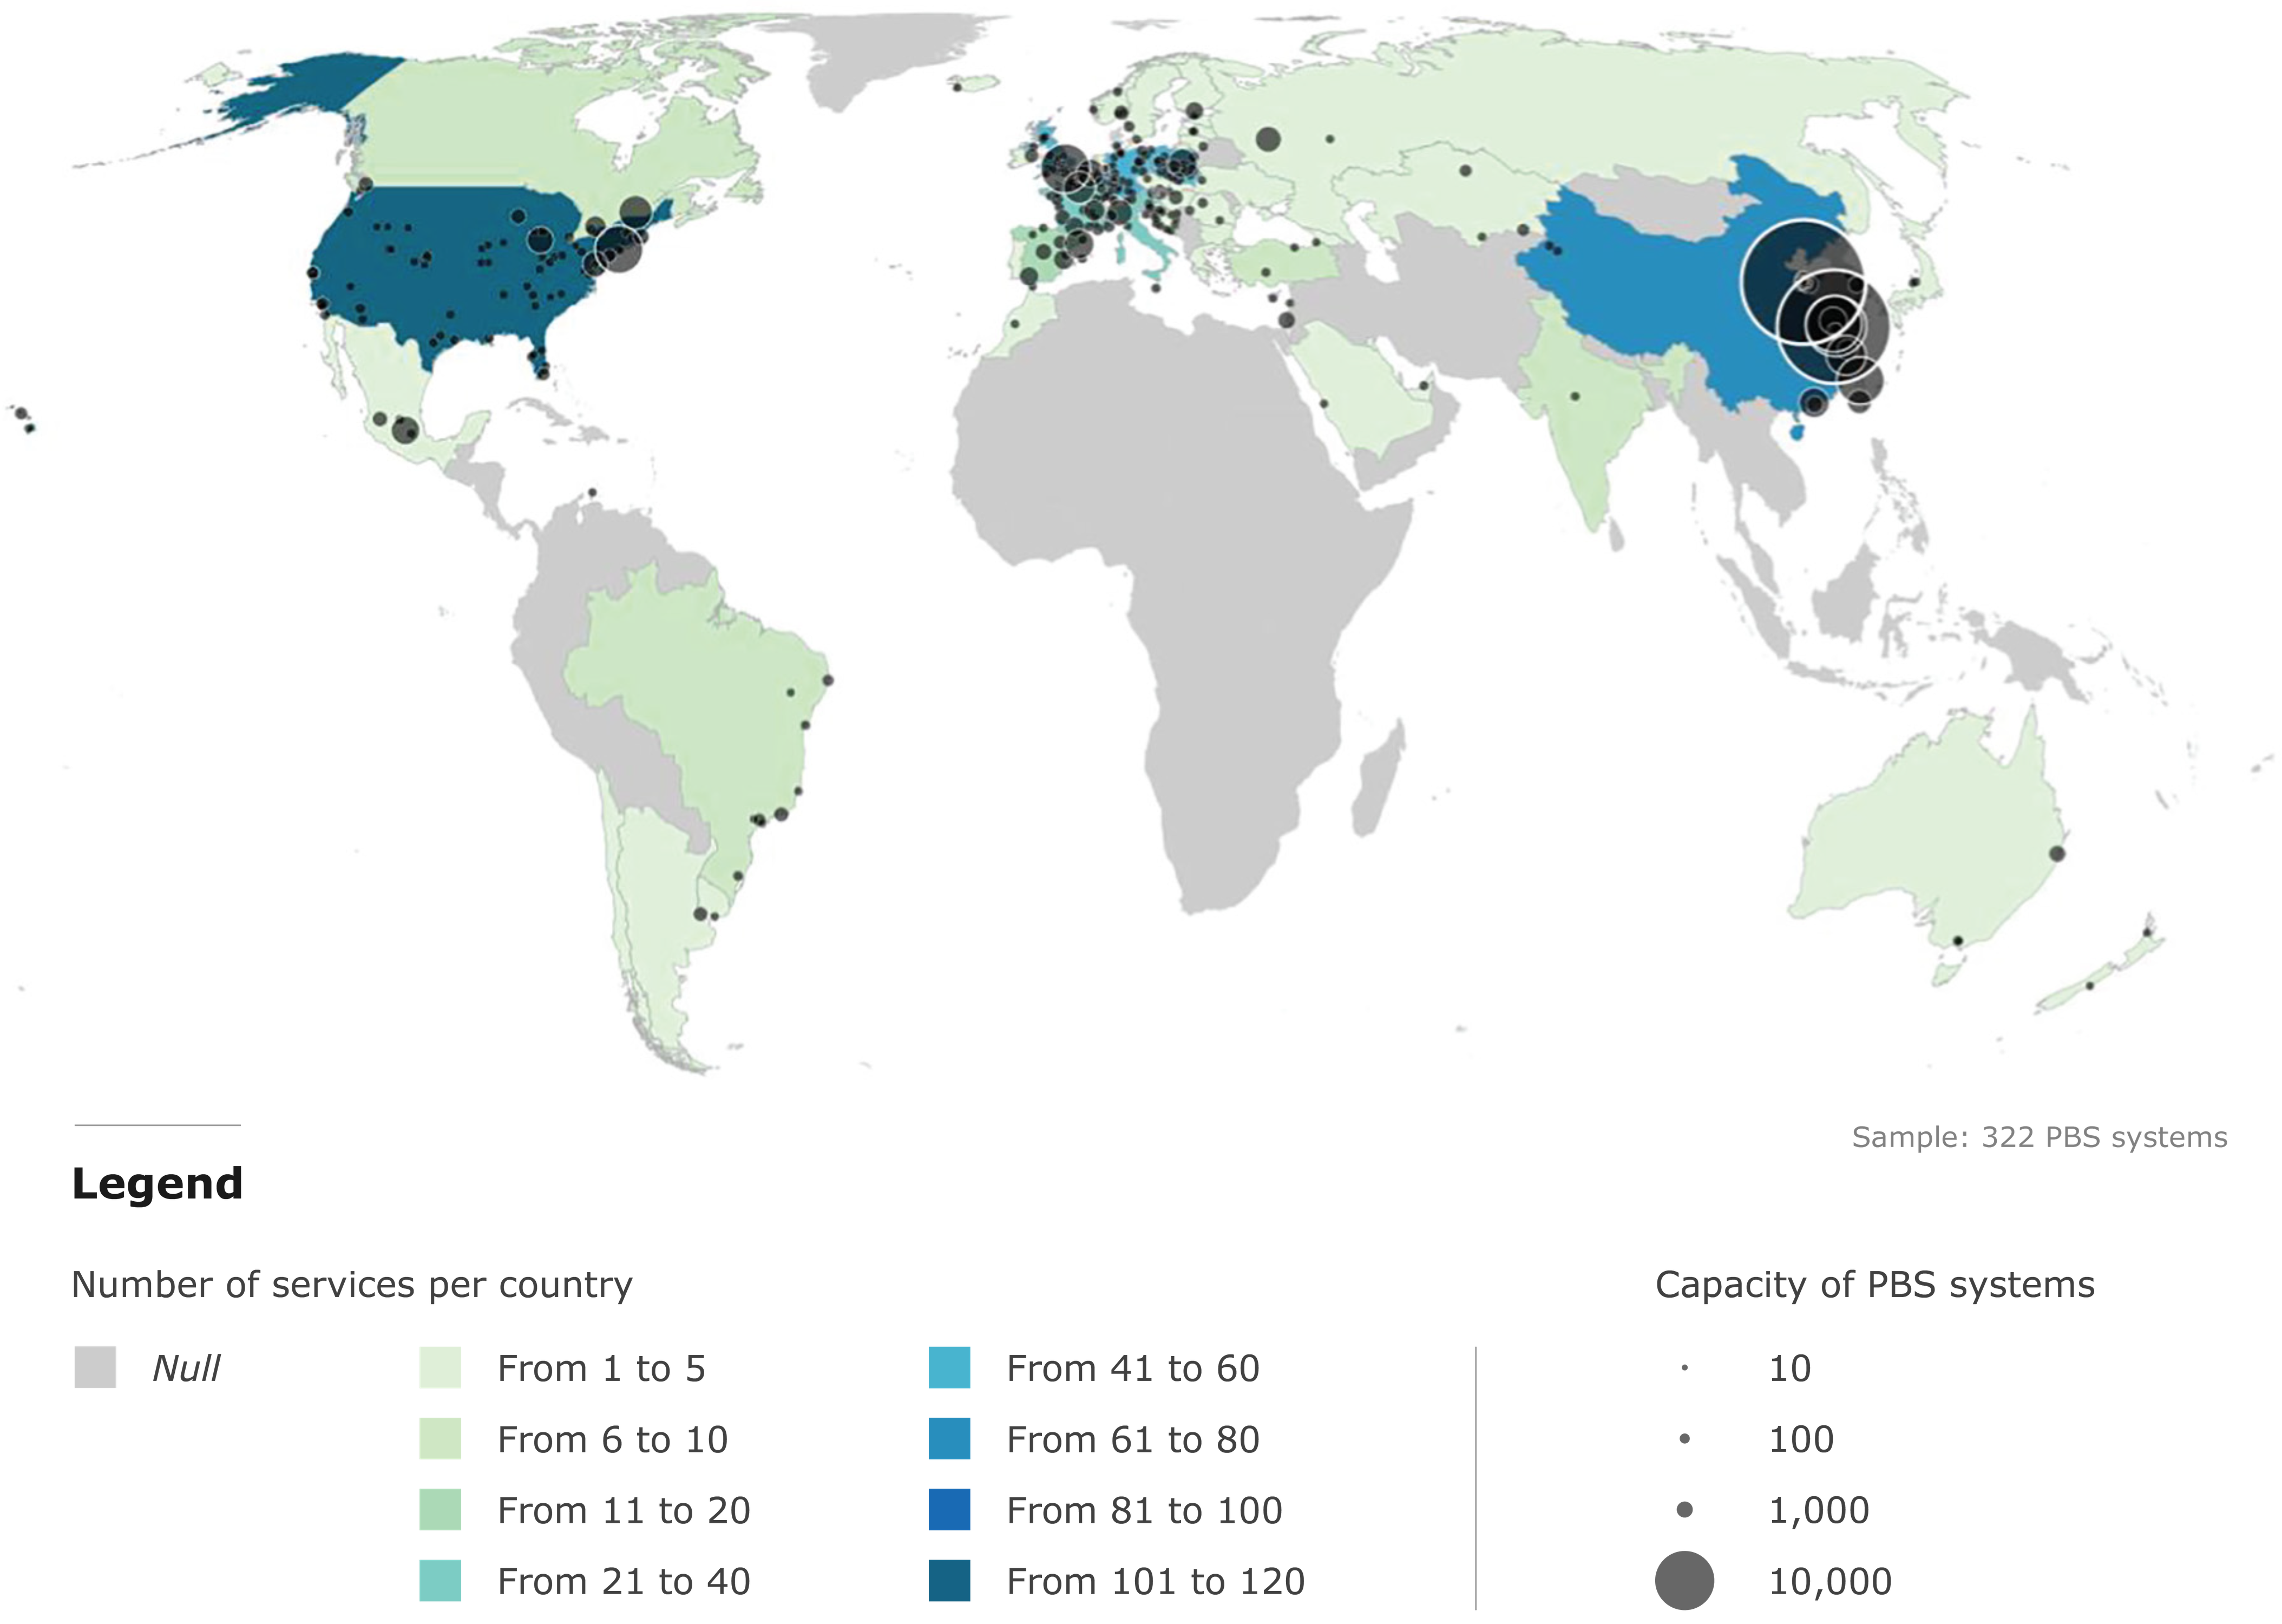
\includegraphics[width=1\columnwidth]{src/Figures/Chap-1/EN_Carte_VLS_monde.png}}
    \vspace{5pt}
    \begin{flushright}\scriptsize{
    Source: \textcolor{blue}{\textcite{todd_global_2021}}\index{Todd, James|pagebf}\index{O'Brien, Oliver|pagebf}\index{Cheshire, James|pagebf}
    \\
    Translation: \textcolor{blue}{Dylan Moinse (2024)}
    }\end{flushright}
\end{carte}

% VFF
While the experience of the \textsl{White Bikes}, \textsl{Call a Bike}, and successive generations of \acrshort{PBS} systems can be seen as the precursors to \acrshort{DBS} systems, their current form truly emerged in China in 2014. That year, \textcolor{blue}{Dai Wei}, a student in Beijing, along with his friends, came up with the idea of a shared bike system designed to facilitate their movement on campus. They founded the startup \Marque{Ofo} after experimenting with bike sharing on their campus \textcolor{blue}{\autocite[10]{nlc_micromobility_2019}}\index{NLC@\textsl{NLC}|pagebf}. This project quickly gained financial support from the Chinese \acrshort{RHS} company \Marque{Didi} \textcolor{blue}{\autocite[18]{6t-bureau_de_recherche_etude_2018}}\index{Bureau de recherche 6t@\textsl{Bureau de recherche 6t}|pagebf}. The service expanded to several Chinese cities before going international. Many Asian \Commas{bike unicorns}\footnote{~
    In 2013, U.S. investor \textcolor{blue}{Aileen Lee} coined the term \Commas{unicorn} to refer to the most highly valued startups in Silicon Valley, California. The mythical animal symbolizes rarity, miracles, and fantasy \textcolor{blue}{\autocite{benner_unicorn_2015}}\index{Benner, Katie|pagebf}. Essentially, it describes a \Commas{\textsl{new technology startup founded less than ten years ago, valued at least one billion dollars before going public.}} \textcolor{blue}{\autocite{chambre_de_commerce_et_dindustrie_licornes_2019}}\index{Chambre de commerce et d'industrie@\textsl{Chambre de commerce et d'industrie}|pagebf}.
} specializing in station-free shared bikes, called \Commas{dockless} sharing system (or \textsl{free-floating}), emerged and expanded their activities to France starting in the fall of 2017. For example, \Marque{Gobee.bike} first deployed its bikes in Lille, followed by Paris a few days later. Within just a few months, five \acrshort{DBS} operators were active in Paris by the end of 2017. Less than a year later, seven \acrshort{DBS} services expanded to eight French cities, with a total fleet of around 15,000 bikes, representing 20\% of shared bikes in the country \textcolor{blue}{\autocite[23]{6t-bureau_de_recherche_etude_2018}}\index{Bureau de recherche 6t@\textsl{Bureau de recherche 6t}|pagebf}. Meanwhile, the two Chinese giants of the sector, \Marque{Ofo} and \Marque{Mobike}, expanded to the 30 largest cities in China, gathering over 200 million users, and also reached 21 other countries \textcolor{blue}{\autocite[22, 91]{kang_university_2020}}\index{Kang, Wei|pagebf}\index{Aguiléra, Anne|pagebf}\index{Rallet, Alain|pagebf}.%%Translated%%

% TEFF
Beyond the description of the vehicle itself, it is primarily the dockless sharing operational model that fuels the discussion on expanding mobility options. Shortly after the deployment of fleets of \acrshort{DBS}, whether mechanical or electric, new services emerge, notably those related to \acrfull{DESS}. Its rise began in 2017 with the creation of the American company \Marque{Bird} by \textcolor{blue}{Travis VanderZanden}, a former executive at \Marque{Lyft} and \Marque{Uber} \textcolor{blue}{\autocite[13]{nlc_micromobility_2019}}\index{NLC@\textsl{NLC}|pagebf}. This project focuses on the revival of the electric scooter, which had been reintroduced a few years earlier \textcolor{blue}{\autocite{easy_electric_life_free_2020}}\index{Easy Electric Life@\textsl{Easy Electric Life}|pagebf}. In France, \acrshort{DESS} services emerged in the summer of 2018, quickly becoming emblematic, alongside \acrshort{DBS}, of the rise of shared mobility \textcolor{blue}{\autocite[1]{bortoli_consequential_2020}}\index{Bortoli, Anne de|pagebf}\index{Christoforou, Zoi|pagebf}. Although shared electric scooter and car services already existed in Europe, the adoption and deployment speed of \acrshort{DESS} systems was unprecedented. For instance, \Marque{Bird} quickly reached \Commas{unicorn} status, and other companies such as \Marque{Lime} (formerly \Marque{LimeBike}) or \Marque{Spin}, originally specialized in \acrshort{DBS}, followed the model in 2018 \textcolor{blue}{\autocite[4]{clewlow_micro-mobility_2018}}\index{Clewlow, Regina|pagebf}. Described as the \Commas{latest form of the Uberization of urban mobility} \textcolor{blue}{\autocite[1]{boffi_extrait_2019}}\index{Boffi, Nicolas|pagebf}, \acrshort{DBS} and \acrshort{DESS} services have set records in terms of diffusion and modal adoption internationally. In Paris, \textcolor{blue}{\textcite[146]{6t-bureau_de_recherche_usages_2019}}\index{Bureau de recherche 6t@\textsl{Bureau de recherche 6t}|pagebf} estimates that, just one year after its launch, \acrshort{DESS} achieved at least a modal share equivalent to that of the \acrshort{PBS} \textsl{Vélib’}, three years after its launch, with an estimate between 0.8\% and 2.2\% of internal trips. In the U.S. and Canada, 39 million \acrshort{DESS} trips were recorded in the first year of service, a number that will double by 2023, despite the COVID-19 health crisis. North American \acrshort{DESS} systems then represent 44\% of shared bike or scooter trips on the continent, a proportion that rises to 49\% in the U.S. \textcolor{blue}{\autocites[10]{nacto_shared_2019}[10]{nacto_shared_2020}[3-5]{nacto_shared_2024}}\index{NACTO@\textsl{NACTO}|pagebf}. One key element, however, distinguishes dockless sharing mobility systems from station-based ones: their geographical distribution. While \acrshort{PBS} services are mainly concentrated in large metropolitan areas, \acrshort{DBS} and \acrshort{DESS} services are deployed in relatively less dense areas.%%Translated%%

% Technologies
Shared mobility, whether in the form of bicycles or scooters, mechanical or electric, is characterized by a common denominator: it frees the user from the costs of acquisition, maintenance, and the responsibilities associated with vehicle ownership \textcolor{blue}{\autocite[44]{mathew_analysis_2019}}\index{Mathew, Jijo|pagebf}\index{Liu, Mingmin|pagebf}\index{Li, Howell|pagebf}\index{Seeder, Sonya|pagebf}\index{Bullock, Darcy|pagebf}. This offering, although diverse, fits into a dynamic of complementarity, but also competition with traditional vehicles. It emerged thanks to a favorable technological context, marked by the commercialization and democratization of recent innovations. First and foremost, the massive diffusion of \textsl{smartphones}\footnote{~
    The \textsl{smartphone}, conceived in 1992, marked a major technological turning point, but it was truly popularized with the release of the \Marque{Iphone} in 2007. By 2008, the \Marque{Iphone 3G} allowed access to the 3G cellular data network, was equipped with GPS functionality, and introduced the use of apps updated through an online store \textcolor{blue}{\autocite{les_numeriques_2007_2014}}\index{Les Numériques@\textsl{Les Numériques}|pagebf}. These advancements profoundly transformed individual behaviors by integrating the \textsl{smartphone} into everyday uses, such as mobile payments (M-payment) or reading \textsl{flashcodes} (\textsl{QR codes}) \textcolor{blue}{\autocites[279]{chaix_paiement_2013}[21]{ben_jaddi_m-paiement_2018}}\index{Chaix, Laetitia|pagebf}\index{Ben Jaddi, Madja|pagebf}. This technological revolution provided fertile ground for the development of shared mobility services, which leverage the five components of the \Commas{\textsl{Internet} of things}, also known as \acrfull{IoT}, namely (i) objects, (ii) the mobile network, (iii) data, (iv) information, and (v) operational applications \textcolor{blue}{\autocite{iot_evolution_world_impact_2017}}\index{IoT Evolution World@\textsl{IoT Evolution World}|pagebf}. Moreover, the widespread adoption of \textsl{smartphones} opened up a huge potential market for these services. The device's democratization was rapid and global. For example, in the United States, the smartphone penetration rate rose from 35\% in 2011 to 77\% in 2018 \textcolor{blue}{\autocite[8]{clewlow_micro-mobility_2018}}\index{Clewlow, Regina|pagebf}. A similar dynamic was observed in France, where this rate went from 17\% in 2011 to 77\% in 2019 \textcolor{blue}{\autocite[28]{credoc_barometre_2019}}\index{CRÉDOC@\textsl{CRÉDOC}|pagebf}.
} enabled \acrfull{STP} to free themselves from the physical anchor of stations. This dematerialization facilitated the implementation of operational models summarized by the saying: \Commas{\textsl{arrive first, ask later}}\footnote{~
    The first generation of shared bike and scooter services, deployed between 2017 and 2020, was characterized by an audacious strategy adopted by operators. They would set up services on territories without prior authorization from local authorities or even informing them, taking advantage of the legal ambiguity surrounding these new mobility services \textcolor{blue}{\autocite{laker_welcome_2019}}\index{Laker, Laura|pagebf}. This tactic was to establish the services \textsl{de facto} before contacting local authorities, aiming to negotiate from a position of strength, thus reducing the necessary concessions \textcolor{blue}{\autocite[5]{lopez-escolano_mobilites_2019}}\index{López-Escolano, Carlos|pagebf}\index{Campos, Ángel Pueyo|pagebf}. The regulatory vacuum regarding the occupation of public space allowed these services to operate without formal agreements \textcolor{blue}{\autocite[5]{lopez-escolano_mobilites_2019}}\index{López-Escolano, Carlos|pagebf}\index{Campos, Ángel Pueyo|pagebf}. This situation led some cities to ban these services, primarily citing two main reasons: illegal occupation of public space and direct competition with existing public transport systems \textcolor{blue}{\autocite[63]{6t-bureau_de_recherche_livre_2019}}. However, these tactics have evolved today. This phase has been replaced by more collaborative approaches, allowing both public and private actors to mutually benefit from these services. Today, operating and regulatory charters govern the implementation of shared mobility services in most major European and North American cities, thus ending unilateral practices and laying the foundations for governance.
}, where operators often caught public authorities off guard. These authorities, historically regulators of urban transport and sometimes operators themselves of services such as \acrshort{PBS}, found themselves in a disadvantageous position against these disruptive actors. Besides the central role of \textsl{smartphones}, geolocation and geofencing also played a strategic role in the deployment of these mobility solutions. Thanks to these technologies, operators can track their fleets in real-time and establish virtual geographic barriers defining the operating areas. However, \acrshort{GPS} technology, with its limited accuracy of 3 to 10 meters depending on the urban environment \textcolor{blue}{\autocite{the_scooterist_dockless_2020}}\index{The Scooterist@\textsl{The Scooterist}|pagebf}, still constitutes a hindrance to fine management of shared vehicles, especially to distinguish between movement or parking on a sidewalk, roadway, or in restricted areas \textcolor{blue}{\autocite[96]{6t-bureau_de_recherche_livre_2019}}\index{Bureau de recherche 6t@\textsl{Bureau de recherche 6t}|pagebf}\footnote{~
    Currently, geolocation of dockless sharing vehicles allows detecting their entry or exit from defined areas, such as expanded parking zones or specific locations like public squares or parks. However, the precision offered by \acrshort{GPS} technology remains limited, not always meeting the expectations of local authorities, who sometimes overestimate its effectiveness as a management solution \textcolor{blue}{\autocite[123]{6t-bureau_de_recherche_livre_2019}}. In response to these limitations, some urban or transport authorities have introduced complementary solutions. These include requiring the user to scan a \textsl{QR code} located in a standardized parking area at the end of the trip, or photographing the parked vehicle as proof of compliance \textcolor{blue}{\autocite[96]{6t-bureau_de_recherche_livre_2019}}.
}. This landscape is expected to evolve with the full operation of the European satellite positioning system \textsl{Galileo}, initiated by the European Union. Partially operational since 2016, this system was finalized at the end of 2024 and is now accessible to the public with free accuracy of about one meter, and centimeter-level accuracy for paid services \textcolor{blue}{\autocite{futura_sciences_galileo_2019}}\index{Futura Sciences@\textsl{Futura Sciences}|pagebf}\index{CNES@\textsl{CNES}|pagebf}. This technological breakthrough opens new prospects for geofencing, not only to improve fleet management and accuracy but also to meet regulatory requirements, especially regarding the parking of shared vehicles.%%Translated%%

 % Semi-floating and Transition
In their \Commas{umbrella review} of shared vehicles, which is a synthesis of 29 existing literature reviews, \textcolor{blue}{\textcite[16]{mangeart_vehicules_2022}}\index{Mangeart, Timothée|pagebf}\index{Bouteuil, Virginie|pagebf} highlight the frequent lack of specific strategies adopted by local authorities regarding shared mobility services. The identified regulatory instruments range from restrictions, public funding, and in-kind benefits, such as the provision of parking spaces. This evolution in public governance is a marker of a profound transformation in the \Commas{socio-technical regime}, driven by the pressure of innovations \textcolor{blue}{\autocites[319]{canitez_pathways_2019}[4]{fryszman_smart_2019}}\index{Canitez, Fatih|pagebf}\index{Fryszman, Flavia|pagebf}\index{Denes Dos Santos Carstens, Danielle|pagebf}\index{Kindl da Cunha, Sieglinde|pagebf}. One of the notable evolutions concerns the organization of \Commas{semi-floating} fleets or \Commas{semi-dockless}, taking the form of either physical or dematerialized stations \textcolor{blue}{\autocite[121]{6t-bureau_de_recherche_livre_2019}}\index{Bureau de recherche 6t@\textsl{Bureau de recherche 6t}|pagebf}. This reflection on \textsl{smartparking} aims to reduce negative externalities, such as inconvenient parking on pedestrian spaces \textcolor{blue}{\autocite[13]{zou_exploratory_2020}}\index{Zhou, Zhenpeng|pagebf}\index{Younes, Hannah|pagebf}\index{Erdoğan, Sevgi|pagebf}\index{Wu, Jiahui|pagebf}. In Paris, for example, the municipality announced in March 2019 that fees imposed on operators would be used to fund 2,500 parking spaces dedicated to \acrshort{DBS} and \acrshort{DESS}\footnote{~
    Parking spaces dedicated to \textsl{dockless sharing} vehicles are often marked on the ground with a specific logo, frequently replacing a car parking space \textcolor{blue}{\autocite{livonniere_trottinettes_2019}}\index{Livonnière, Stanislas de|pagebf}. These spaces are typically sized to accommodate six \acrshort{DESS}, for example \textcolor{blue}{\autocite{burban_trottinettes_2019}}\index{Burban, Thibault|pagebf}. This measure makes sense with the municipal decree of July 30, 2019, which prohibits the parking of \acrshort{DBS} and \acrshort{DESS} on sidewalks. The text specifies: \Commas{\textsl{Considering that, under these conditions, it is necessary to organize the parking of these vehicles to ensure pedestrian safety and guarantee good walking conditions, restricting parking possibilities to only those places adapted to their geometric and functional characteristics.}} \textcolor{blue}{\autocite[3151]{ville_de_paris_bulletin_2019}}. This initiative complements an application and strategic reinterpretation of Article 52 of the 2019 \acrfull{LOM}, which states that parking spaces for cars located within five meters of pedestrian crossings will be neutralized before 2027 to ensure better visibility for pedestrians \textcolor{blue}{\autocite[42]{gart_loi_2020}}. To date, around 2,500 reserved parking spaces have been created in the capital, representing a total of 15,000 spaces for \acrshort{DBS} and \acrshort{DESS}.
} \textcolor{blue}{\autocites[3151]{ville_de_paris_bulletin_2019}[90]{6t-bureau_de_recherche_livre_2019}}\index{Bureau de recherche 6t@\textsl{Bureau de recherche 6t}|pagebf}\index{Ville de Paris@\textsl{Ville de Paris}|pagebf}. Reminiscent of the pioneering operation model of the Danish \acrshort{DBS} company \Marque{Donkey Republic}\footnote{~
    Facing competition from massive Asian and North American operators, the Danish company \Marque{Donkey Republic} entered the Parisian market in 2018 with a fleet of 250 \acrshort{DBS} \textcolor{blue}{\autocite[20]{6t-bureau_de_recherche_etude_2018}}. What distinguishes \Marque{Donkey Republic} from its competitors is its \Commas{hybrid} approach, halfway between \acrshort{PBS} and \acrshort{DBS} systems \textcolor{blue}{\autocite[20]{6t-bureau_de_recherche_etude_2018}}. Unlike classic dockless sharing models, \Marque{Donkey Republic} uses existing urban furniture, such as bike racks, to offer a structured parking system. At the end of a ride, the user is required to lock the shared bike to one of these racks using chains provided by the operator \textcolor{blue}{\autocite[20]{6t-bureau_de_recherche_etude_2018}}. Although this model somewhat restricts the user's freedom by imposing specific parking locations, it offers several advantages. On the one hand, it helps limit theft risks, and on the other hand, it prevents the chaotic parking issues often associated with dockless sharing systems and the damages they cause. This first system, which introduces a certain discipline into shared vehicle usage, constitutes a form of self-regulation by the operator. It also lays the foundations for broader reflection on regulating dockless fleets in urban spaces.
}. This evolution occurs in a context where \acrshort{STP} are responding to growing demands for immediacy, flexibility, and freedom of use \textcolor{blue}{\autocite[8]{frere_services_2018}}\index{Frère, Séverine|pagebf}\index{Castex, Élodie|pagebf}\index{Mathon, Sylvie|pagebf}. More broadly, the resurgence of cycles and scooters reflects a revival of the paradigm around proximity and the ideal of the \Commas{compact city}, promoting active modes and functional diversity as alternatives to urban sprawl \textcolor{blue}{\autocite[44]{eskenazi_voir_2022}}\index{Eskenazi, Manon|pagebf}. This shift reflects contemporary social changes, marked by the dissolution of traditional structures in favor of increased flexibility \textcolor{blue}{\autocite[130-142]{bauman_liquid_2000}}\index{Bauman, Zygmunt|pagebf}.%%Translated%%

% 1.2.3.
\needspace{1\baselineskip} % Reserve space
\subsection{Characterization of a Class of Vehicles Linked to \Commas{Light Individual Mobility,} a Symbol of a Renewed Interest in Proximity
    \label{chap1:caracterisation-mobilite-individuelle-legere}
    }

    % Introduction
In contemporary societies, the values associated with the search for flexibility and adaptability, combined with those of individualism and immediacy, have profoundly redefined our mobility practices and, consequently, transformed the existing mobility offer. This quest for \Commas{fluidity,} characterized by a gradual retreat of fixed collective structures in favor of ever-moving interaction networks \textcolor{blue}{\autocite[19-24]{bauman_liquid_2000}}\index{Bauman, Zygmunt|pagebf}, has coupled with the commercialization of technological innovations adopted by the latest \Commas{connected} and \Commas{nomadic} generations. It has thus fostered growing demand for the renewal of mobility systems, adapted to mobile consumption and a rediscovery of proximity \textcolor{blue}{\autocite[103-108]{bu_tout-voiture_2024}}\index{Bu, Ludovic|pagebf}. In this context, diversification, along with the modal hybridization of cycles, emerges as a response to contemporary aspirations, articulated around demands for efficiency, resilience, proximity, and energy and economic sobriety. This family of vehicles encompasses a range of modes, from the classic bicycle to personal or shared mobility devices. However, their growth and increasing appeal make it difficult, even today, to conceptually define these categories, notably due to the heterogeneity of the definitions associated with them. These semantic ambiguities have led us to adopt an expanded definition of what we call \Commas{light individual mobility,} a term borrowed from the research project \textcolor{blue}{\textcite{urfe_projet_2022}}\index{URFé@\textsl{URFé}|pagebf}. From this perspective, we propose our own definition, aiming to group light individual vehicles while going beyond existing classifications. Within this category, it is still possible to distinguish two main subcategories: on the one hand, the bicycle and its variations, and on the other hand, \Commas{micromobility,} taking the legal definition of the \acrfull{PMD}, regardless of their type of propulsion or mode of acquisition.%%Translated%%

% 1.2.3.1.
\needspace{1\baselineskip} % Reserve space
\subsubsection*{On the Traces of the \Commas{Liquidity} of Movement
    \label{chap1:mobilite-individuelle-legere-contexte-societes-liquides}
    }

    % Introduction
The technical innovations we have explored are not, by themselves, sufficient to explain the favorable context for the emergence of cycles, whether mechanical or electric, owned or shared. These innovations are part of a larger process where they intersect with new practices and social aspirations, deeply rooted in contemporary social and economic changes that redefine daily mobility. Contemporary society is marked by a rise in individualism and an increasing quest for fluidity and flexibility, reflecting new needs. In this regard, British and Polish philosopher and sociologist \textcolor{blue}{Zygmunt} \textcolor{blue}{\textcite[7-28]{bauman_liquid_2000}}\index{Bauman, Zygmunt|pagebf}, in his book *Liquid Life*, develops the idea of \Commas{liquid societies} (\textsl{Liquid Modernity})\footnote{~
    The theory of \Commas{liquid society} (\textsl{Liquid Modernity}) developed by \textcolor{blue}{Zygmunt} \textcolor{blue}{\textcite[7-28]{bauman_liquid_2000}}\index{Bauman, Zygmunt|pagebf} describes a world where solid collective structures, which once founded social organization and promoted interactions grounded in common institutions, are weakening in favor of a fluidity centered on the individual. Unlike the \Commas{solid society,} where individuals co-construct stable and durable social frameworks, the \Commas{liquid society} relies on ephemeral relationships, individualized choices, and ubiquitous consumption as drivers of social relations and identities. In this society, the individual becomes an entity in perpetual movement, defined not by fixed statuses or stable social ties, but by an ability to rapidly adapt to changes and consume flexibly. As \textcolor{blue}{Agnès} \textcolor{blue}{\textcite[2]{falabregues_bauman_2014}}\index{Falabrègues, Agnès|pagebf} summarizes, liquid life is caught in an incessant flow of mobility and speed, where consumerism triumphs as a structuring principle. Life rhythms thus become synonymous with constant movement, valorizing individual freedom while weakening collective solidarities. This constantly flowing economy requires consumption services, such as mobility, to be highly adaptable, customizable, and flexible to meet the growing demands of consumers for flexibility. In this perspective, shared mobility services fit perfectly into this logic, offering instantaneous solutions tailored to individual needs and freed from ownership constraints. They embody the idea of mobile consumerism, where each individual can access a vehicle according to their needs, without long-term commitment or excessive responsibility, fluctuating with preferences and circumstances. The author then calls for \Commas{intelligent cooperation,} where the economy and innovations would serve the public interest. As \textcolor{blue}{Robert} \textcolor{blue}{\textcite{maggiori_zygmunt_2017}}\index{Maggiori, Robert|pagebf} recalls, he invites us to rethink social organization so that it is not solely at the service of individual consumerism but oriented toward common and sustainable goals.
}, where he observes the central role of technological innovations. According to him, postmodern societies rely less on fixed structures, but more on \Commas{networks of human interactions}, characterized by their ability to connect and disconnect with disarming ease \textcolor{blue}{\autocite{philosophie_science_et_societe_modernite_2017}}\index{Philosophie, science et société@\textsl{Philosophie, science et société}|pagebf}. This paradigm reflects a moving and adaptable social environment, conducive to the emergence of shared mobility services. In this context, the intensification of life rhythms, the explosion of social networks, and the omnipresence of \acrshort{ICT} have redefined social interaction modes and mobility practices. These are transformations that will give rise to shared services, which meet the demands of a society seeking quick, flexible, and adaptive solutions \textcolor{blue}{\autocite[44]{mathew_analysis_2019}}\index{Mathew, Jijo|pagebf}\index{Liu, Mingmin|pagebf}\index{Li, Howell|pagebf}\index{Seeder, Sonya|pagebf}\index{Bullock, Darcy|pagebf}.%%Translated%%

% Mobility
According to the French researcher and futurist \textcolor{blue}{Georges} \textcolor{blue}{\textcite[13]{amar_homo_2016}}\index{Amar, Georges|pagebf}, the contemporary paradigm summarized as \Commas{everyone has their own mobility} deeply redefines movement dynamics by introducing a key figure: the \textsl{homo mobilis}. This refers to a \Commas{\textsl{mobile, multimodal, and communicative person, a designer and co-producer of their own mobility}}. This paradigm marks a turning point by moving away from the old priorities centered on the performance of \textsl{transit}—the triptych of speed, capacity, and range \textcolor{blue}{\autocite[207]{sheller_new_2006}}\index{Sheller, Mimi|pagebf}\index{Urry, John|pagebf}—to focus on immaterial aspects such as accessibility, interfaces, places, and interactions. \textcolor{blue}{Georges} \textcolor{blue}{\textcite[14]{amar_homo_2016}}\index{Amar, Georges|pagebf} refers to this renewed dimension of mobility as \Commas{the immobile part of transport}. The conceptual formulation of \Commas{mobility reliance}, as developed by him, characterizes the transition towards mobility aimed at creating connections, synergies, and opportunities, going beyond the simple function of overcoming distances. This reliance is largely based on \Commas{\textsl{proximity mobilities}} \textcolor{blue}{\autocite[103, 222]{amar_homo_2016}}\index{Amar, Georges|pagebf}, which rearticulate spatial scales by promoting accessibility \Commas{\textsl{through proximity}} to resources, amenities, and urban infrastructures \textcolor{blue}{\autocites{marzloff_trottinette_2019}[2]{silva_proximity-centred_2023}}\index{Marzloff, Bruno|pagebf}\index{Silva, Cecília|pagebf}\index{Büttner, Benjamin|pagebf}\index{Seisenberger, Sebastian|pagebf}\index{Rauli, Anna|pagebf}. Reliance becomes the new value of mobility and territories \textcolor{blue}{\autocite[12, 99]{amar_homo_2016}}\index{Amar, Georges|pagebf}. It can directly echo the \textsl{Hybrid Transit Metropolises}, which are less rigid and linear, reinventing their spatial organization by adapting to these \Commas{mega-trends} identified by \textcolor{blue}{\textcite[133]{cervero_transit_2020}}\index{Cervero, Robert|pagebf}. These trends reflect profound structural changes, including: a diversification of \textsl{living}; a reconfiguration of forms and places of production; a heterogeneity of ways of moving and the spaces and times invested; as well as new values, mainly carried by the latest generations.%%Translated%%

% New Generations' Aspirations
As summarized by \textcolor{blue}{Todd} \textcolor{blue}{\textcite[29]{litman_current_2012}}\index{Litman, Todd|pagebf}, founder of the \textsl{Victoria Policy Institute}, an independent institute specializing in transportation research, the expectations of new generations sharply contrast with those of the \textsl{Baby Boomers}. While for the latter, owning a house and a car represented both status and symbolic goals, the following generations tend to prioritize alternative forms of satisfaction, often centered on the use of electronic devices and a more pragmatic relationship with mobility. This phenomenon is not limited to age, but rather reflects a real socio-cultural shift, where the car loses its central role in favor of less costly, more flexible, and modular modes of transport \textcolor{blue}{\autocite{peaslee_one_2021}}\index{Peaslee, Emma|pagebf}. From an economic, practical, and symbolic point of view, the behaviors of generations \textsl{Y} and \textsl{Z}, followed by generation \textsl{Alpha}\footnote{~
    The term \Commas{generations} helps capture the demographic and sociological dynamics influencing individual and collective behaviors. Derived from the generational theory developed by \textcolor{blue}{\textcite{strauss_generations_1992}}\index{Howe, Neil|pagebf}\index{Strauss, William|pagebf}, these demographic cohorts are defined by temporal criteria related to birth years and are characterized by shared experiences and values. A generation is thus defined as a \Commas{\textsl{cohort-group whose length approximates the span of a phase of life and whose boundaries are fixed by peer personality},} where \Commas{peer personality} refers to a \Commas{\textsl{recognized generational identity determined by common age location; common beliefs and behavior; and perceived membership in a common generation}} \textcolor{blue}{\autocite[60, 64]{strauss_generations_1992}}\index{Howe, Neil|pagebf}\index{Strauss, William|pagebf}. In the current \textsl{saeculum}, that of the \Commas{Millennials}, multiple generations coexist, each with distinct practices and representations regarding mobility \textcolor{blue}{\autocite[31-57]{howe_millennials_2000}}\index{Howe, Neil|pagebf}\index{Strauss, William|pagebf}, although their boundaries continue to evolve and be debated \textcolor{blue}{\autocite[3]{wang_bike_2018}}\index{Wang, Kailai|pagebf}\index{Akar, Gulsah|pagebf}\index{Chen, Yu-Jen|pagebf}:
        \begin{customitemize}
    \item \textsl{Baby Boomers} (between 1945 and 1965): Associated with the peak of automobile use, this generation continues to heavily rely on this mode of transport. However, the aging of this cohort gradually reduces their car usage;
    \item \textsl{Xennials} or \textsl{Generation~X} (between 1965 and 1980): Less dependent on cars than the \textsl{Baby Boomers}, they still use motor vehicles extensively;
    \item \textsl{Millennials} or \textsl{Generation~Y} (between 1980 and 2000): Representing a generational shift, they own and use fewer cars. Their relationship with driving licenses and car ownership tends to decline in favor of multimodal or shared solutions;
    \item \textsl{Zoomers} or \textsl{Generation~Z} (between 2000 and 2010) and \textsl{Alpha} (between 2010 and 2020): These generations seem to embody a more pragmatic approach to mobility. Naturally multimodal, they prioritize adaptability depending on the context of travel. Less attached to the car as a symbol, they favor diverse and combined solutions.
        \end{customitemize}
}, are oriented towards increased use of connected devices and opportunistic mobility forms, often at the expense of car ownership \textcolor{blue}{\autocite[25]{litman_future_2020}}\index{Litman, Todd|pagebf}. Mobility is being reinvented in the form of \Commas{modal hybridization}, combining the strengths of public transport and individual modes, and stimulating a diversification of mobility behaviors \textcolor{blue}{\autocite[20]{amar_du_2012}}\index{Amar, Georges|pagebf}. Driven by new values \textcolor{blue}{\autocite{lacombled_smart_2014}}\index{Lacombled, David|pagebf}\index{Jeanneau, Christian|pagebf}, this shift in the balance of power against the car promotes a generation of mobile and connected individuals, socializing in an environment transformed by the advent of the \acrshort{IoT}. Their relationship with mobility is oriented toward utilitarian and flexible solutions, integrated into connected and horizontal networks \textcolor{blue}{\autocite{bloomberg_citylab_clearest_2015}}\index{Bloomberg CityLab@\textsl{Bloomberg CityLab}|pagebf}. This generational upheaval occurs in a context where individuals' lifestyle expectations are reshaping mobility models in contemporary societies \textcolor{blue}{\autocites{circella_what_2016}{garikapati_activity_2016}{tilley_multi-level_2017}}\index{Garikapati, Venu~M.|pagebf}\index{Pendyala, Ram~M.|pagebf}\index{Morris, Eric~A.|pagebf}\index{Mokhtarian, Patricia~L.|pagebf}\index{McDonald, Noreen|pagebf}\index{Tilley, Sara|pagebf}\index{Circella, Giovanni|pagebf}\index{Tiedeman, Kate|pagebf}\index{Handy, Susan~L.|pagebf}\index{Alemi, Farzard|pagebf}.%%Translated%%

% Mobility Implications - Generations + Transition
It has been demonstrated that the \textsl{Millennials} generation, and even more so the \textsl{digital natives} of subsequent generations, tend to use cars less, are fewer in number with a driving license, and prioritize multimodality more. This is explained by a renewed interest in public transport, cycling, and \acrshort{PBS}, as well as a lower tendency to live in suburban areas \textcolor{blue}{\autocites[62-63]{polzin_impact_2014}[32-39]{circella_what_2016}{garikapati_activity_2016}[7]{hntb_america_2016}[9-10]{alfaraz_youth_2017}[12]{wang_bike_2018}}\index{Alfaraz, Claudio|pagebf}\index{Tully, Claus|pagebf}\index{Garikapati, Venu~M.|pagebf}\index{Pendyala, Ram~M.|pagebf}\index{Morris, Eric~A.|pagebf}\index{Mokhtarian, Patricia~L.|pagebf}\index{McDonald, Noreen|pagebf}\index{Circella, Giovanni|pagebf}\index{Tiedeman, Kate|pagebf}\index{Handy, Susan~L.|pagebf}\index{Alemi, Farzard|pagebf}\index{Wang, Kailai|pagebf}\index{Akar, Gulsah|pagebf}\index{Chen, Yu-Jen|pagebf}\index{Polzin, Steven~E.|pagebf}\index{Chu, Xuehao|pagebf}\index{Godfrey, Jodi|pagebf}\index{HNTB@\textsl{HNTB}|pagebf}. The enthusiasm for alternative mobility systems reflects an aspiration for lifestyles focused on proximity and accessibility \textcolor{blue}{\autocite[99-100]{levine_mobility_2019}}\index{Levine, Jonathan|pagebf}\index{Grengs, Joe|pagebf}\index{Merlin, Louis~A.|pagebf}. This trend is manifested by the emergence of communities like the one gathered on the \Marque{Facebook} page \acrfull{NUMTOT}, which has over 230,000 members and serves as both a forum for critical and humorous discussion, mocking modern urbanism and the \Commas{car-centric} mentality \autocites{bliss_future_2018}{demain_la_ville_numtot_2018}\index{Bliss, Laura|pagebf}\index{Demain La Ville@\textsl{Demain La Ville}|pagebf}. Primarily driven by the latest generations, individuals are turning away from cars in favor of cheaper and equally personalized alternatives, thus opening significant opportunities for both individual and collective alternatives that can address these needs for freedom, proximity, and efficiency \textcolor{blue}{\autocite[11]{frere_services_2018}}\index{Frère, Séverine|pagebf}\index{Castex, Élodie|pagebf}\index{Mathon, Sylvie|pagebf}. These social trends highlight the need to clearly define the boundaries of the vehicles that make up the alternative mobility system. In this perspective, it is essential to clarify the scope of this family of cycles. This framing and terminology exercise will serve as a guiding thread for the reflections carried out throughout this work.%%Translated%%

% 1.2.3.2.
\needspace{1\baselineskip} % Reserved space
\subsubsection*{Towards an Attempt to Define Light Individual Mobility
    \label{chap1:mobilite-individuelle-legere-definition}
    }

% Introduction
Faced with the growing diversity of modes of transportation encompassing bicycles, scooters, and other technical and social objects, both English- and French-language scientific literature seem to struggle to agree on the boundaries for defining this family of vehicles. However, these modes theoretically share common characteristics: they are classified as \Commas{light,} individual, rely on the ability to maintain balance, and use wheels for movement. Furthermore, these vehicles are positioned \textsl{a priori} as intermediate solutions between walking and heavy motorized modes such as cars or public transport. However, some ambiguity persists regarding the numerous terms used to describe them. For example, the term \Commas{micromobility} (or micromobility) tends to exclude bicycles, which are considered less compact than scooters \textcolor{blue}{\autocite[2, 4]{litman_new_2021}}\index{Litman, Todd|pagebf}, while \Commas{active modes,} referring only to \Commas{self-propelled} mobilities \textcolor{blue}{\autocite{illich_energie_1973}}\index{Illich, Ivan|pagebf}\index{Giard, Luce|pagebf}\index{Bardet, Vincent|pagebf}, or \Commas{soft mobility} \footnote{~
    It should be noted that we prefer to use the term \Commas{active mobility} to describe walking and cycling, rather than \Commas{soft mobility,} which has an ambiguous meaning. The latter term can also refer to some motorized, collective, non-thermal, or non-strictly individual mobilities, such as carpooling, depending on personal interpretations \textcolor{blue}{\autocite[240-241]{demailly_mobilite_2021}}\index{Demailly, Kaduna-Eve|pagebf}\index{Monnet, Jérôme|pagebf}\index{Scapino, Julie|pagebf}\index{Deraëve, Sophie|pagebf}\index{Demade, Julien|pagebf}.
} includes walking and cycling but excludes motorized vehicles \textcolor{blue}{\autocite[555]{adam_mobilite_2020}}\index{Adam, Matthieu|pagebf}, leaving the debate open for assisted vehicles like \acrshort{e-Bike}. Moreover, terms like \acrfull{NIEV}, \acrfull{LPEV}, and \acrfull{PLEV} tend to marginalize vehicles powered solely by human energy, such as the classic bicycle \textcolor{blue}{\autocite[4]{pages_nouveaux_2021}}\index{Pages, Thibaud|pagebf}\index{Lammoglia, Adrien|pagebf}\index{Josselin, Didier|pagebf}. In the \textsl{Dictionnaire pluriel de la marche en ville}, \textcolor{blue}{Jérôme} \textcolor{blue}{\textcite[233]{demailly_micro-vehicules_2021}}\index{Demailly, Kaduna-Eve|pagebf}\index{Monnet, Jérôme|pagebf}\index{Scapino, Julie|pagebf}\index{Deraëve, Sophie|pagebf}\index{Monnet, Jérôme|pagebf} proposes referring to these vehicles as \Commas{\gls{micro-vehicles}} in order to emphasize their three distinct characteristics: objects that carry only one person, with reduced speed and nuisances; that must be driven and parked; and that provide an advantage for intermodality. A typology proposed by \textcolor{blue}{Frédéric} \textcolor{blue}{\textcite[40]{heran_nouvelles_2018}}\index{Héran, Frédéric|pagebf} differentiates \Commas{micromobility,} which includes scooters and folding bicycles, from \Commas{alternative mobility,} which includes city bicycles and \acrshort{e-Bike}. Beyond terminological debates, \acrfull{PMD} and \acrfull{ePMD} \footnote{~
    An \acrfull{ePMD} is a recent category of vehicles officially recognized by the Highway Code and defined by Decree No. 2019-1082 of October 23, 2019, concerning the regulation of personal mobility devices. According to paragraph 6.15 of Article 3 of this decree, a \acrshort{ePMD} is defined as a \Commas{\textsl{vehicle without a seat, designed and constructed for the transportation of one person only and lacking any provision for carrying goods, equipped with a non-thermal motor or non-thermal assistance, and whose maximum speed by construction is greater than 6 km/h and does not exceed 25 km/h} [\dots] \textsl{Vehicles intended exclusively for persons with reduced mobility are excluded from this category}} \textcolor{blue}{\autocite{legifrance_decret_2019}}\index{Légifrance@\textsl{Légifrance}|pagebf}. This definition emphasizes the specific characteristics of \acrshort{ePMD}, namely their non-thermal motorization, individual use, and limited speed, while explicitly excluding devices intended for people with reduced mobility. In parallel, the broader category associated with \acrfull{PMD} is marked by a less restrictive approach, which is not limited to electrically assisted motorized vehicles. This more inclusive definition has the advantage of anticipating technological developments in mobility, such as the development of new energies, particularly hydrogen, or the revaluation of human forces (human energy) as a means of propulsion \textcolor{blue}{\autocite{mobilityurban_quest-ce_2019}}\index{Mobilityurban@\textsl{Mobilityurban}|pagebf}. This conceptual flexibility allows for the integration of a variety of vehicles into a regulatory framework that is likely to evolve with technological progress and emerging practices.
} fall within a recent regulatory framework, which, however, has the limitation of excluding the bicycle and its many variants, as they are not strictly considered \Commas{vehicles} in the traditional sense.%%Translated%%

% Description MIL
As we can observe, no terminology seems truly appropriate for describing all of these vehicles in their diversity without introducing some confusion. However, it seems regrettable to segment or differentiate modes of transportation that, by nature, respond to similar challenges by mobilizing common characteristics. These vehicles indeed embody an alternative transportation system that does not rely on a fixed route, as is the case with public transport, nor on a service model dependent on dedicated infrastructure and centralized management, like \acrfull{DRT}. They thus contribute to a mobility system that consumes few resources, approaching the ideal of \Commas{sustainable mobility} \textcolor{blue}{\autocite[5]{itdp_electric_2019}}\index{ITDP@\textsl{ITDP}|pagebf}, while incorporating the principles of \Commas{transmodality.} These objects capture the functional benefits associated with automobilities\footnote{~
    Cycles share values associated with \Commas{\Commas{automobility}} \textcolor{blue}{\autocites[57-58]{urry_sociology_2000}[28]{urry_system_2004}}\index{Urry, John|pagebf}, such as the sense of freedom, flexibility, and independence, as well as technical elements like infrastructure, which characterize automobile driving \textcolor{blue}{\autocite[12]{heran_reduction_2001}}\index{Héran, Frédéric|pagebf}.
}, while fully contributing to the development of alternative mobility or \Commas{eco-mobility transition} \textcolor{blue}{\autocites[25]{amar_homo_2016}{heran_transition_2018}}\index{Amar, Georges|pagebf}\index{Héran, Frédéric|pagebf}. Nevertheless, the aforementioned terminologies tend to exclude certain often invisibilized vehicles, even though they are commonly used, such as the mechanical scooter, roller skates, or even the skateboard \textcolor{blue}{\autocite[19]{sebban_complementarite_2003}}\index{Sebban, Annie-Claude|pagebf}\index{Motte, Alain|pagebf}. Furthermore, the desire to exclude walking from this family of vehicles is based on the distinction of a different relationship to mobility: walking does not require the use of a mechanical device, unlike the other modes considered. This distinction also raises the question of the environmental advantage of bicycles and scooters, which can only be truly significant if they do not exclusively replace walking \textcolor{blue}{\autocite[12]{dezobry_du_2020}}\index{Dezobry, Guillaume|pagebf}\index{Fontenelle, Louis de|pagebf}\index{Staropoli, Carine|pagebf}. This differentiation thus helps clarify the relationships between walking, on the one hand, and heavy vehicles such as cars or public transport, on the other hand. The issue is also to provide some nuance regarding the \Commas{intermediate vehicles}\footnote{~
    \Commas{Intermediate modes} encompass a wide variety of vehicles located between the weight of a bicycle and that of a car, while sharing similar domains of relevance. This category includes \acrshort{e-Bike}, the \textsl{speed pedelec} classified among mopeds, as well as various special bicycles such as cargo cycles, recumbent bikes, velomobiles, tandems, folding bicycles, or even bike-cars. It also includes more compact motorized vehicles such as microcars, mini-cars, or cars without a license, as well as two-wheelers, tricycles, or protected motorized quadricycles, not to mention mini-cars \textcolor{blue}{\autocites{bigo_malus_2020}{heran_avenir_2022}[2]{bigo_quelle_2024}}\index{Bigo, Aurélien|pagebf}\index{Héran, Frédéric|pagebf}.
To date, the most developed intermediate vehicles correspond to those at the extremes of this spectrum, namely, on the one hand, \acrshort{e-Bike}, very close to a classic bicycle, and on the other hand, the electric quadricycle, like the \Marque{Citroën Ami}, which resembles a car more. In contrast, vehicles truly intermediate between a bicycle and a car, such as velomobiles or bike-cars, are still in the prototype stage or in the early phases of production in France, showing ongoing but still limited development \textcolor{blue}{\autocite{bigo_vehicules_2023}}\index{Bigo, Aurélien|pagebf}.
}, positioned between the bicycle and the car, which have begun to emerge and are gradually being recognized in recent years \textcolor{blue}{\autocites{bigo_malus_2020}{heran_avenir_2022}[12]{bigo_quelle_2024}}\index{Bigo, Aurélien|pagebf}\index{Héran, Frédéric|pagebf}. These vehicles, particularly the larger ones, cannot be classified as objects of \Commas{urban glide,} which is the main focus of our analysis. Thus, our positioning in this semantic dialogue lies at the interface between the place of walking and that of intermediate and motorized vehicles.%%Translated%%

% Figure définition périmètre micro-mobilité
\begin{figure}[h!]\vspace*{4pt}
    \caption{Definition perimeter of \Commas{light individual mobility} encompassing the bicycle and \Commas{micromobility.}}
    \label{fig-chap1:perimetre-micromobilite}
    \centerline{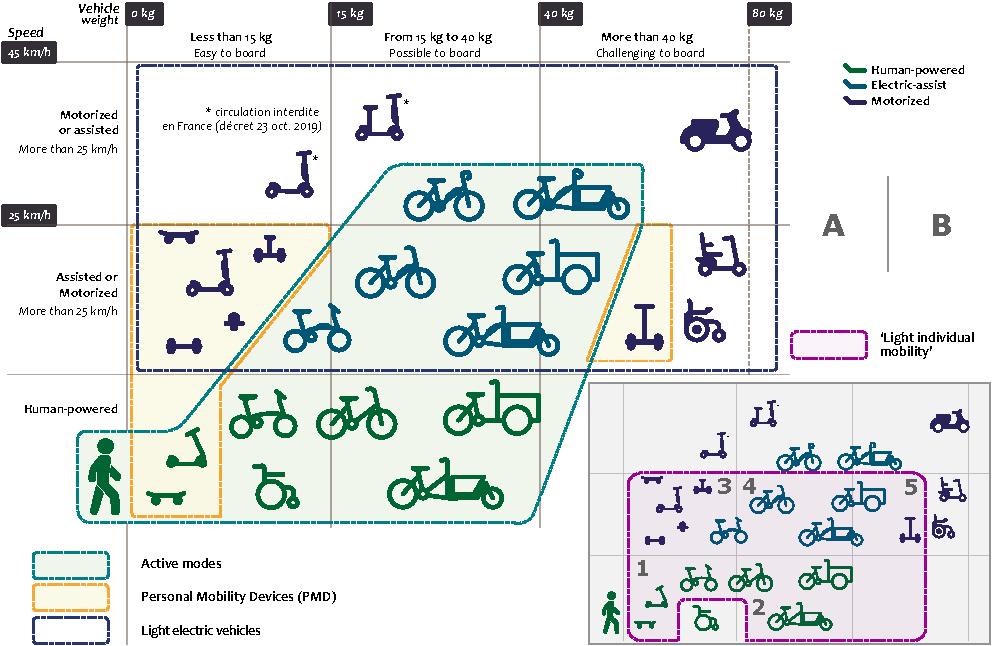
\includegraphics[width=1\columnwidth]{src/Figures/Chap-1/EN_Definition_perimetre_micromobilite.pdf}}
    \vspace{5pt}
    \begin{flushright}\scriptsize{
    Source (A): \textcolor{blue}{\textcite[61]{rabaud_quand_2022}}\index{Rabaud, Mathieu|pagebf}\index{Richer, Cyprien|pagebf}
    \\
    Graphic adaptation (B): \textcolor{blue}{Dylan Moinse (2023)}
    }\end{flushright}
\end{figure}

% Définition MIL
In this context, we propose to adopt an expression that we believe is more suitable for defining the scope of these diverse vehicles, while avoiding confusion related to the inclusion of walking or heavy vehicles. This reflection is based on the work of the ANR project \acrfull{URFé}\footnote{~
    The project, lasting 42 months, is organized into three components whose intersection allows for verifying the hypothesis of a gap between actual mobility practices and spatial planning logic: (i) the uses, effective practices, and safety issues, (ii) the built environment and its potential for accommodating low environmental impact mobility, and (iii) spatial planning as a public action through the lens of low environmental impact mobility \textcolor{blue}{\autocite{urfe_projet_2022}}.
}, under the scientific responsibility of \textcolor{blue}{Frédérique Hernandez}. This research project examines the hospitality of urban space towards new forms of low environmental impact mobility, using the urban areas of Lyon, Lausanne, Marseille–Aix-en-Provence, and Strasbourg as study areas \textcolor{blue}{\autocite{urfe_projet_2022}}\index{URFé@\textsl{URFé}|pagebf}. Although the expression \Commas{low environmental impact individual mobility modes,} used in this project, also has its limitations, in our view, regarding the precise delineation of the vehicles involved, we have chosen to adopt another concept from this research: that of \Commas{light individual mobility.} This expression was emphasized during the fourth collective seminar of the \acrshort{URFé} project, held on November 9, 2022, at \acrshort{Cerema} Hauts-de-France, and it seems particularly relevant for grouping the objects under study. Drawing inspiration from the framework proposed by \textcolor{blue}{\textcite[61]{rabaud_quand_2022}}\index{Rabaud, Mathieu|pagebf}\index{Richer, Cyprien|pagebf} in their chapter titled \Commas{When Personal Transport Devices Transform Urban Mobility,} and in relation to \hyperref[fig-chap1:perimetre-micromobilite]{Figure~\ref{fig-chap1:perimetre-micromobilite}} (page~\pageref{fig-chap1:perimetre-micromobilite}), we propose a definition perimeter for \Commas{light individual mobility} that goes beyond the frameworks of \Commas{active modes,} \acrshort{PMD}, \Commas{light electric vehicles,} and \Commas{intermediate vehicles.} This perimeter aims to include vehicles related to bicycles, micromobility, and their many variants. Our definition is based on partial inclusion of the \gls{active modes}, excluding walking, as well as \acrshort{PMD}, which exclude vehicles specifically designed for people with reduced mobility and some intermediate vehicles whose speeds exceed the regulatory limits for personal transport devices. Thus, \Commas{light individual mobility} encompasses a non-exhaustive list of popular vehicles (see \hyperref[fig-chap1:perimetre-micromobilite]{Figure~\ref{fig-chap1:perimetre-micromobilite}}, page~\pageref{fig-chap1:perimetre-micromobilite}):
    \begin{customitemize}
\item Muscular energy vehicles weighing less than 15 kilograms (cell 1), such as the skateboard, mechanical scooter, or folding bicycle;
\item Muscular energy vehicles weighing between 15 and 40 kilograms (cell 2), such as the classic bicycle, cargo bike (or biporteur), or tricycle;
\item Electric vehicles weighing less than 15 kilograms, with a maximum speed of 25 km/h (cell 3), such as the hoverboard, monowheel, \acrshort{PeS}, or electric unicycle;
\item Electric assist vehicles weighing between 15 and 40 kilograms, with a maximum speed of 25 km/h (cell 4), such as the folding electric bicycle, \acrshort{e-Bike}, electric cargo bike (or electric biporteur), or electric tricycle;
\item Electric vehicles weighing more than 40 kilograms, with a maximum speed of 25 km/h (cell 5), such as the segway;
\item Shared bikes and micromobility services, short or long-term rentals, with or without docking stations (cells 1 to 5), such as folding bikes in free service, \acrshort{PBS}, \acrshort{DESS}, \acrshort{e-Bike} in dockless sharing or service, electric cargo bikes in free service, or the segway for rent.
    \end{customitemize}%%Translated%%

% Transition
Within this family of \Commas{light individual mobility,} we maintain the subcategories associated with bicycles and their various derivatives, such as the folding bicycle, \acrshort{e-Bike}, or cargo bike, as well as \Commas{micromobility,} which primarily refers to the family of \acrshort{PMD}. These vehicles share a number of common characteristics: they are individual modes of transport, although some \Commas{intermediate modes} can accommodate an additional passenger. Their speed is limited, which allows for a form of proximity and interaction with the urban environment, fitting within the spirit of a \textsl{slow city} \textcolor{blue}{\autocite[103-108]{bu_tout-voiture_2024}}\index{Bu, Ludovic|pagebf}. Furthermore, these modes of transport are characterized by their low cost and their more inclusive nature, as they do not require a driving license, making them accessible to a wide range of users. They rely on a common system, conceptualized under the name \Commas{velomobility,} structured around a triptych based on territories, individuals, and uses \textcolor{blue}{\autocites[20-21]{rerat_au_2019}[492]{watson_how_2012}}\index{Rérat, Patrick|pagebf}\index{Watson, Matt|pagebf}. These vehicles, by nature, have potential for intermodality: they are either easily transportable in public transport or easily adapted for parking near a public transport hub. It is due to these various qualities that we will now focus more closely on the synergies between our two main objects of study: public transport and light individual mobility, drawing on the theoretical and strategic framework of \acrshort{TOD}. This approach will allow us to examine how \acrshort{TOD} can appropriate not only bicycles, as briefly explored in the context of \Commas{Hybrid Transit Metropolises} such as Copenhagen, but also the implications arising from the recent diversification of light individual mobility offerings. Through this analysis, we aim to highlight the synergetic links between these two systems.%%Translated%%

% 1.3.
\newpage
\needspace{1\baselineskip} % Reserve space
\sectionheader{Towards a \textsl{Micromobility-friendly Transit-Oriented Development}}
\section{New Perspectives for a \textsl{Transit-Oriented Development} Supported by the Integration of Light Individual Mobility
    \label{chap1:btod}
    }

    % Introduction
The improvement of scientific knowledge related to the development of public transport infrastructures has shown that they are not, by themselves, sufficient to form a viable alternative to \Commas{car dependency}\footnote{~
    \Commas{Car dependency} refers to the practice of traveling by car alone. It is derived from the term \Commas{autosolisme}. A political dictionary defines this term as \Commas{the act of traveling alone in a car, thus congesting the collective space, polluting, making noise, stressing for the benefit of a single person: the driver!} \textcolor{blue}{\autocite{carfreeEN_dictionnaire_2008}}\index{Carfree.fr@\textsl{Carfree.fr}|pagebf}. Occasionally, the antonym \Commas{carpooling} might be used, but it is more common to refer to \Commas{carpooling.}
}, across all areas \textcolor{blue}{\autocite[8]{molino_pratiques_2015}}\index{Molino, Marie|pagebf}\index{Rampon, Anne-Sophie|pagebf}\index{Cipolla, Romain|pagebf}. The traditional development of public transport supply requires simultaneous action on demand. Indeed, to effectively reduce car traffic, several strategies can be considered. One option is to reduce the urbanized area, which is difficult to achieve and accept. Another is to increase public transport coverage, which, however, could undermine the network's performance due to the high number of stops, thus compromising its competitiveness against the car. A more realistic option is to improve station accessibility \textcolor{blue}{\autocite[10]{verbavatz_critical_2019}}\index{Verbavatz, Vincent|pagebf}\index{Barthelemy, Marc|pagebf}. Research shows that the determining factor for the modal shift from car to public transport is accessibility to stations, rather than the qualitative improvement of the service \textcolor{blue}{\autocite[146]{brons_access_2009}}\index{Brons, Martijn|pagebf}\index{Givoni, Moshe|pagebf}\index{Rietveld, Piet|pagebf}. This observation aligns with the founding principle that mobility within transit-oriented neighborhoods, and especially prioritizing walking and cycling combined, constitutes a central lever for the success of a \acrshort{TOD} intervention. However, these modes of transport, while essential to public transport-oriented urban planning, are often overlooked or treated trivially, even though they play a decisive role in the success or failure of a \acrshort{TOD} project \textcolor{blue}{\autocite[34]{schlossberg_comparing_2004}}\index{Schlossberg, Marc|pagebf}\index{Brown, Nathaniel|pagebf}. Due to suburban sprawl, the performance and attractiveness of public transport networks have considerably diminished, due to longer distances and the dispersion of employment centers \textcolor{blue}{\autocite[13]{bentayou_transit-oriented_2015}}\index{Bentayou, Gilles|pagebf}. In this context, the intermodal approach incorporating cycling appears to be the most appropriate solution to address the challenges of the \Commas{first and last miles.} Cycling and public transport must thus maintain a symbiotic relationship: beyond just a feeder mode, cycling must be fully integrated into the travel experience, due to the strong competitiveness of this modal combination against the private car \textcolor{blue}{\autocite[208]{kager_characterisation_2016}}\index{Kager, Roland|pagebf}\index{Bertolini, Luca|pagebf}\index{te Brömmelstroet, Marco|pagebf}. Beyond cycling itself, it is now worth evaluating whether the \Commas{new mobility} modes that revolve around it can strengthen this dynamic. These emerging modes could indeed fit into a \Commas{bundle of modes and services} designed to maximize the benefits of a more resource-efficient alternative mobility system \textcolor{blue}{\autocite[134]{litman_new_2021}}\index{Litman, Todd|pagebf}.%%Translated%%

% Announcement of the plan
First, we will explore the arbitrary rule of walkable perimeter areas around \acrshort{TOD}\textcolor{blue}{s} and, more broadly, the need to expand transit-oriented neighborhoods through an intermodal approach. We will see that studies show how combined walking can extend far beyond the geographical perimeter usually attributed to it, while emphasizing that its reach, although relevant, remains insufficient to ensure optimal access to transport hubs in a suburbanization context. It thus appears essential to integrate other modes of transport that allow reaching more distant destinations, in order to enhance modal complementarity and optimize accessibility to hubs (\hyperref[chap1:btod-limites-tod]{section on a reinterpretation of combined walking, page~\pageref{chap1:btod-limites-tod}}). In this perspective, we will examine the comparative advantages of light individual mobility, which appears as a particularly suitable alternative to limit excessive reliance on cars. This reflection will lead us to discuss the recent development of a \acrfull{B-TOD}, or transit-oriented development integrating cycling, which highlights the potential of bicycles in extending the influence areas of public transport stations. Finally, in light of the modal diversity discussed earlier in this chapter, we will question the value of a more inclusive conceptualization integrating light individual mobility, through an \acrfull{M-TOD} (\hyperref[chap1:btod-definition]{section on a modal combination leveraging speed and \Commas{door-to-door} accessibility, page~\pageref{chap1:btod-definition}}).%%Translated%%

% 1.3.1.
\needspace{1\baselineskip} % Reserve space
\subsection{\Commas{Bursting the Bubble} of Pedestrian Pockets
    \label{chap1:btod-limites-tod}
    }

    % Introduction
The concept of \Commas{pedestrian pocket}, which predates \acrshort{TOD}, is based on the demarcation of an area within which walking is the preferred mode of transport, and where the main daily activities are concentrated \textcolor{blue}{\autocite[3]{kelbaugh_pedestrian_1989}}\index{Kelbaugh, Doug|pagebf}. Although widely integrated into the concept of urban planning, the pedestrian influence area of stations is often defined by arbitrary boundaries that do not necessarily reflect the actual practices of travelers, potentially resulting in a mismatch between the station neighborhood perimeter and the actual travel paths of users. From this observation, we align with recent scientific literature calling for a reconsideration of the real reach of combined walking. Indeed, pedestrian pathways to and from a station do not stop at the immediate scale of the station, but also influence the spatiotemporal distance users are willing to travel \textcolor{blue}{\autocite[52]{el_hadeuf_ville_2017}}\index{El Hadeuf, Mounya|pagebf}\index{Laterrasse, Jean|pagebf}. In this perspective, we propose to use this \Commas{bursting of the bubble} \textcolor{blue}{\autocite[33]{guerra_half-mile_2012}}\index{Guerra, Erick|pagebf} as an opportunity to redefine spatial planning by adopting a systemic or integrative approach \textcolor{blue}{\autocite[56]{kaufmann_retour_2014}}\index{Kaufmann, Vincent|pagebf} to highlight the advantages of intermodal travel. Such an approach would allow the development of spaces truly oriented towards public transport, defined on a more relevant spatial scale and likely to optimize modal shift towards the public transport network.%%Translated%%

% 1.3.1.1.
\needspace{1\baselineskip} % Reserve space
\subsubsection*{Questioning the \textsl{Doxa} of Confined \Commas{Pedestrian Pockets}
    \label{chap1:btod-limites-tod-marche-restreinte}
    }

    % Doxa
In France, as we have observed, we often witness the implementation of principles close to \Commas{\acrshort{TOD} without saying so} \textcolor{blue}{\autocite[273]{lo_feudo_scenario_2014}}\index{Lo Feudo, Fausto|pagebf}\index{Menerault, Philippe|pagebf}\index{L'Hostis, Alain|pagebf}\index{Festa, Demetrio Carmine|pagebf}. This multiplicity of interventions in the territory, related to this concept of urban planning, is often limited to punctual actions such as architectural renewal of stations or the redevelopment of adjacent spaces, giving less attention to larger scales, particularly the station neighborhood and its integration into the metropolitan area \textcolor{blue}{\autocite[50]{bentayou_transit-oriented_2015}}\index{Bentayou, Gilles|pagebf}. When \acrshort{TOD}\textcolor{blue}{s} specifically target the pedestrian influence areas of public transport nodes, they rely on a commonly accepted reference: that of 500 meters or 800 meters, the latter equating to 10 minutes of walking \textcolor{blue}{\autocite[1]{lhostis_perimetres_2016}}\index{L'Hostis, Alain|pagebf}, often defined as a \Commas{\textsl{Pedestrian Pocket}}. \textcolor{blue}{Peter} \textcolor{blue}{\textcite[56]{calthorpe_next_1993}}\index{Calthorpe, Peter|pagebf} recommends communities designed within 600 meters (approximately 2,000 feet) of a stop. \textcolor{blue}{\textcite[12]{bertolini_cities_2015}}\index{Bertolini, Luca|pagebf}\index{Spit, Tejo|pagebf}, in their book \foreignlanguage{english}{\textsl{Cities on Rails: The Redevelopment of Railway Stations and their Surroundings}} confirm that a 10-minute walking radius is an acceptable time-distance for accessing a station. A literature review on action perimeters around stations, conducted by \textcolor{blue}{\textcite[102]{guerra_half-mile_2012}}\index{Guerra, Erick|pagebf}\index{Cervero, Robert|pagebf}\index{Tischler, Daniel|pagebf}, shows, however, that this norm of 400 to 800 meters is frequently used without necessarily being backed by technical justifications. Yet, as we have seen in the evolution of \acrshort{TOD} thinking, one of the \Commas{5Ds} associated with this concept, distance to stations (\textsl{Distance to Transit}), is a central equation for measuring accessibility to public transport \textcolor{blue}{\autocite[267]{ewing_travel_2010}}\index{Ewing, Reid|pagebf}\index{Cervero, Robert|pagebf}. Over the past decade, research has sought to question this international standard of \Commas{800 meters} (\textsl{half-mile distance}), which has become a standard in \acrshort{TOD}\textcolor{blue}{s} \textcolor{blue}{\autocite[102]{guerra_half-mile_2012}}\index{Guerra, Erick|pagebf}\index{Cervero, Robert|pagebf}\index{Tischler, Daniel|pagebf}. The goal is to \Commas{burst the pedestrian bubble} \textcolor{blue}{\autocite[33]{guerra_half-mile_2012}}\index{Guerra, Erick|pagebf}, meaning to exceed the limits of the combined walking radius. This opens the way to a reinterpreted \acrshort{TOD} model, going beyond the spatial metaphor of the \Commas{bull’s eye} \textsl{(the bull’s eye concept)} \textcolor{blue}{\autocite[28]{curtis_transit_2009}}\index{Curtis, Carey|pagebf}\index{Renne, John Luciano|pagebf}\index{Bertolini, Luca|pagebf}.%%Translated%%

% Urban planning documents
This commonly accepted rule, based on the 800-meter pedestrian perimeter, is frequently applied and visible in the urban planning guidelines. Urban planners typically use this limit as the action perimeter around stations \textcolor{blue}{\autocite[40]{olszewski_using_2005}}\index{Olszewski, Piotr~S.|pagebf}\index{Wibowo, Sony Sulaksono|pagebf}. Already in the \textsl{Regional Transport Scheme} of the former \textcolor{blue}{\textcite[21]{region_nord-pas-de-calais_schema_2006}}\index{Région Nord-Pas-de-Calais@\textsl{Région Nord-Pas-de-Calais}|pagebf}, walking was identified as a mode to prioritize for short-distance feeder trips to bus or coach stops, train stations, and interchange hubs. The \acrfull{PDU} 2010-2020 of the \acrfull{MEL} incorporated this approach by defining \acrfull{DIVAT}, corresponding to strategic areas located around metropolitan stations, subway and tramway stations, as well as \acrfull{BRT} stops. These strategic perimeters were then shaped into a 500-meter radius circle \textcolor{blue}{\autocite[39]{lmcu_plan_2011}}\index{LMCU@\textsl{LMCU}|pagebf}. In line with this \acrshort{PDU}, the \acrshort{DIVAT} were faithfully incorporated into the \acrfull{PLH} 2012-2018 of the \acrshort{MEL}, with an extension to bus stops recording more than sixty daily passages in all directions \textcolor{blue}{\autocite[4]{lmcu_2e_2012}}\index{LMCU@\textsl{LMCU}|pagebf}. These principles were then integrated into the 2020 \acrfull{PLUi} of the \acrfull{EPCI}, thereby enhancing the consistency between the various territorial planning tools \textcolor{blue}{\autocite[44]{metropole_europeenne_de_lille_plan_2019-3}}\index{LMCU@\textsl{LMCU}|pagebf}. However, some strategic studies have revisited these station perimeters to adapt them to varied contexts. For example, the Grand Paris Express station observatory initially defined an 800-meter bird's-eye view perimeter for the 69 stations under construction \textcolor{blue}{\autocite[1]{apur_observatoire_2017}}\index{Apur@\textsl{Apur}|pagebf}. This framework was later evolved to propose two additional levels: 500 meters for stations in the city center and 1,000 meters for \acrfull{RER} stations and those of the Grand Paris Express \textcolor{blue}{\autocite[13]{apur_observatoire_2018}}\index{Apur@\textsl{Apur}|pagebf}. Finally, particular attention was given to a 2,000-meter radius for the cycling scale \textcolor{blue}{\autocite[22]{apur_observatoire_2018}}\index{Apur@\textsl{Apur}|pagebf}.%%Translated%%

% Expansion of primary areas
Some consider that combined walking can reach spatio-temporal distances well beyond those dictated by the Anglo-Saxon rule of 400 or 800 meters, or even 10 minutes, within the perimeter of the \Commas{primary area} as imagined by \textcolor{blue}{Peter} \textcolor{blue}{\textcite[56]{calthorpe_next_1993}}\index{Calthorpe, Peter|pagebf}. In a literature review, the researcher in geography, specializing in planning and mobility, \textcolor{blue}{Alain} \textcolor{blue}{\textcite[5]{lhostis_perimetres_2016}}\index{L'Hostis, Alain|pagebf} highlights that some European train stations or metro stations record walking distances easily reaching one to two kilometers. The practice of combined walking (\textsl{walk-and-ride}) around well-served transport hubs, benefiting from high frequencies, extensive coverage, and good accessibility, is thus marked by an extension of its socially accepted distances. These neighborhoods, which are both dense, mixed, and feature high-quality public space design, particularly in terms of \gls{walkability}, embody the principles of \acrshort{TOD} neighborhoods \textcolor{blue}{\autocites[79]{ker_myths_2003}[7]{lhostis_perimetres_2016}[30]{hasiak_access_2019}}\index{Hasiak, Sophie|pagebf}\index{L'Hostis, Alain|pagebf}\index{Ker, Ian|pagebf}\index{Ginn, Simon|pagebf}. Research shows that in this context, walking trips far exceed the traditionally accepted 800-meter threshold \textcolor{blue}{\autocites[79]{ker_myths_2003}[7]{lhostis_perimetres_2016}[30]{hasiak_access_2019}}\index{Hasiak, Sophie|pagebf}\index{L'Hostis, Alain|pagebf}\index{Ker, Ian|pagebf}\index{Ginn, Simon|pagebf}.%%Translated%%

% Pedestrian Corridor
\begin{carte}[h!]\vspace*{4pt}
    \caption{Extension of the station area through the enhancement of a densified and walkable corridor.}
    \label{fig-chap1:tod-corridor-pieton}
    \centerline{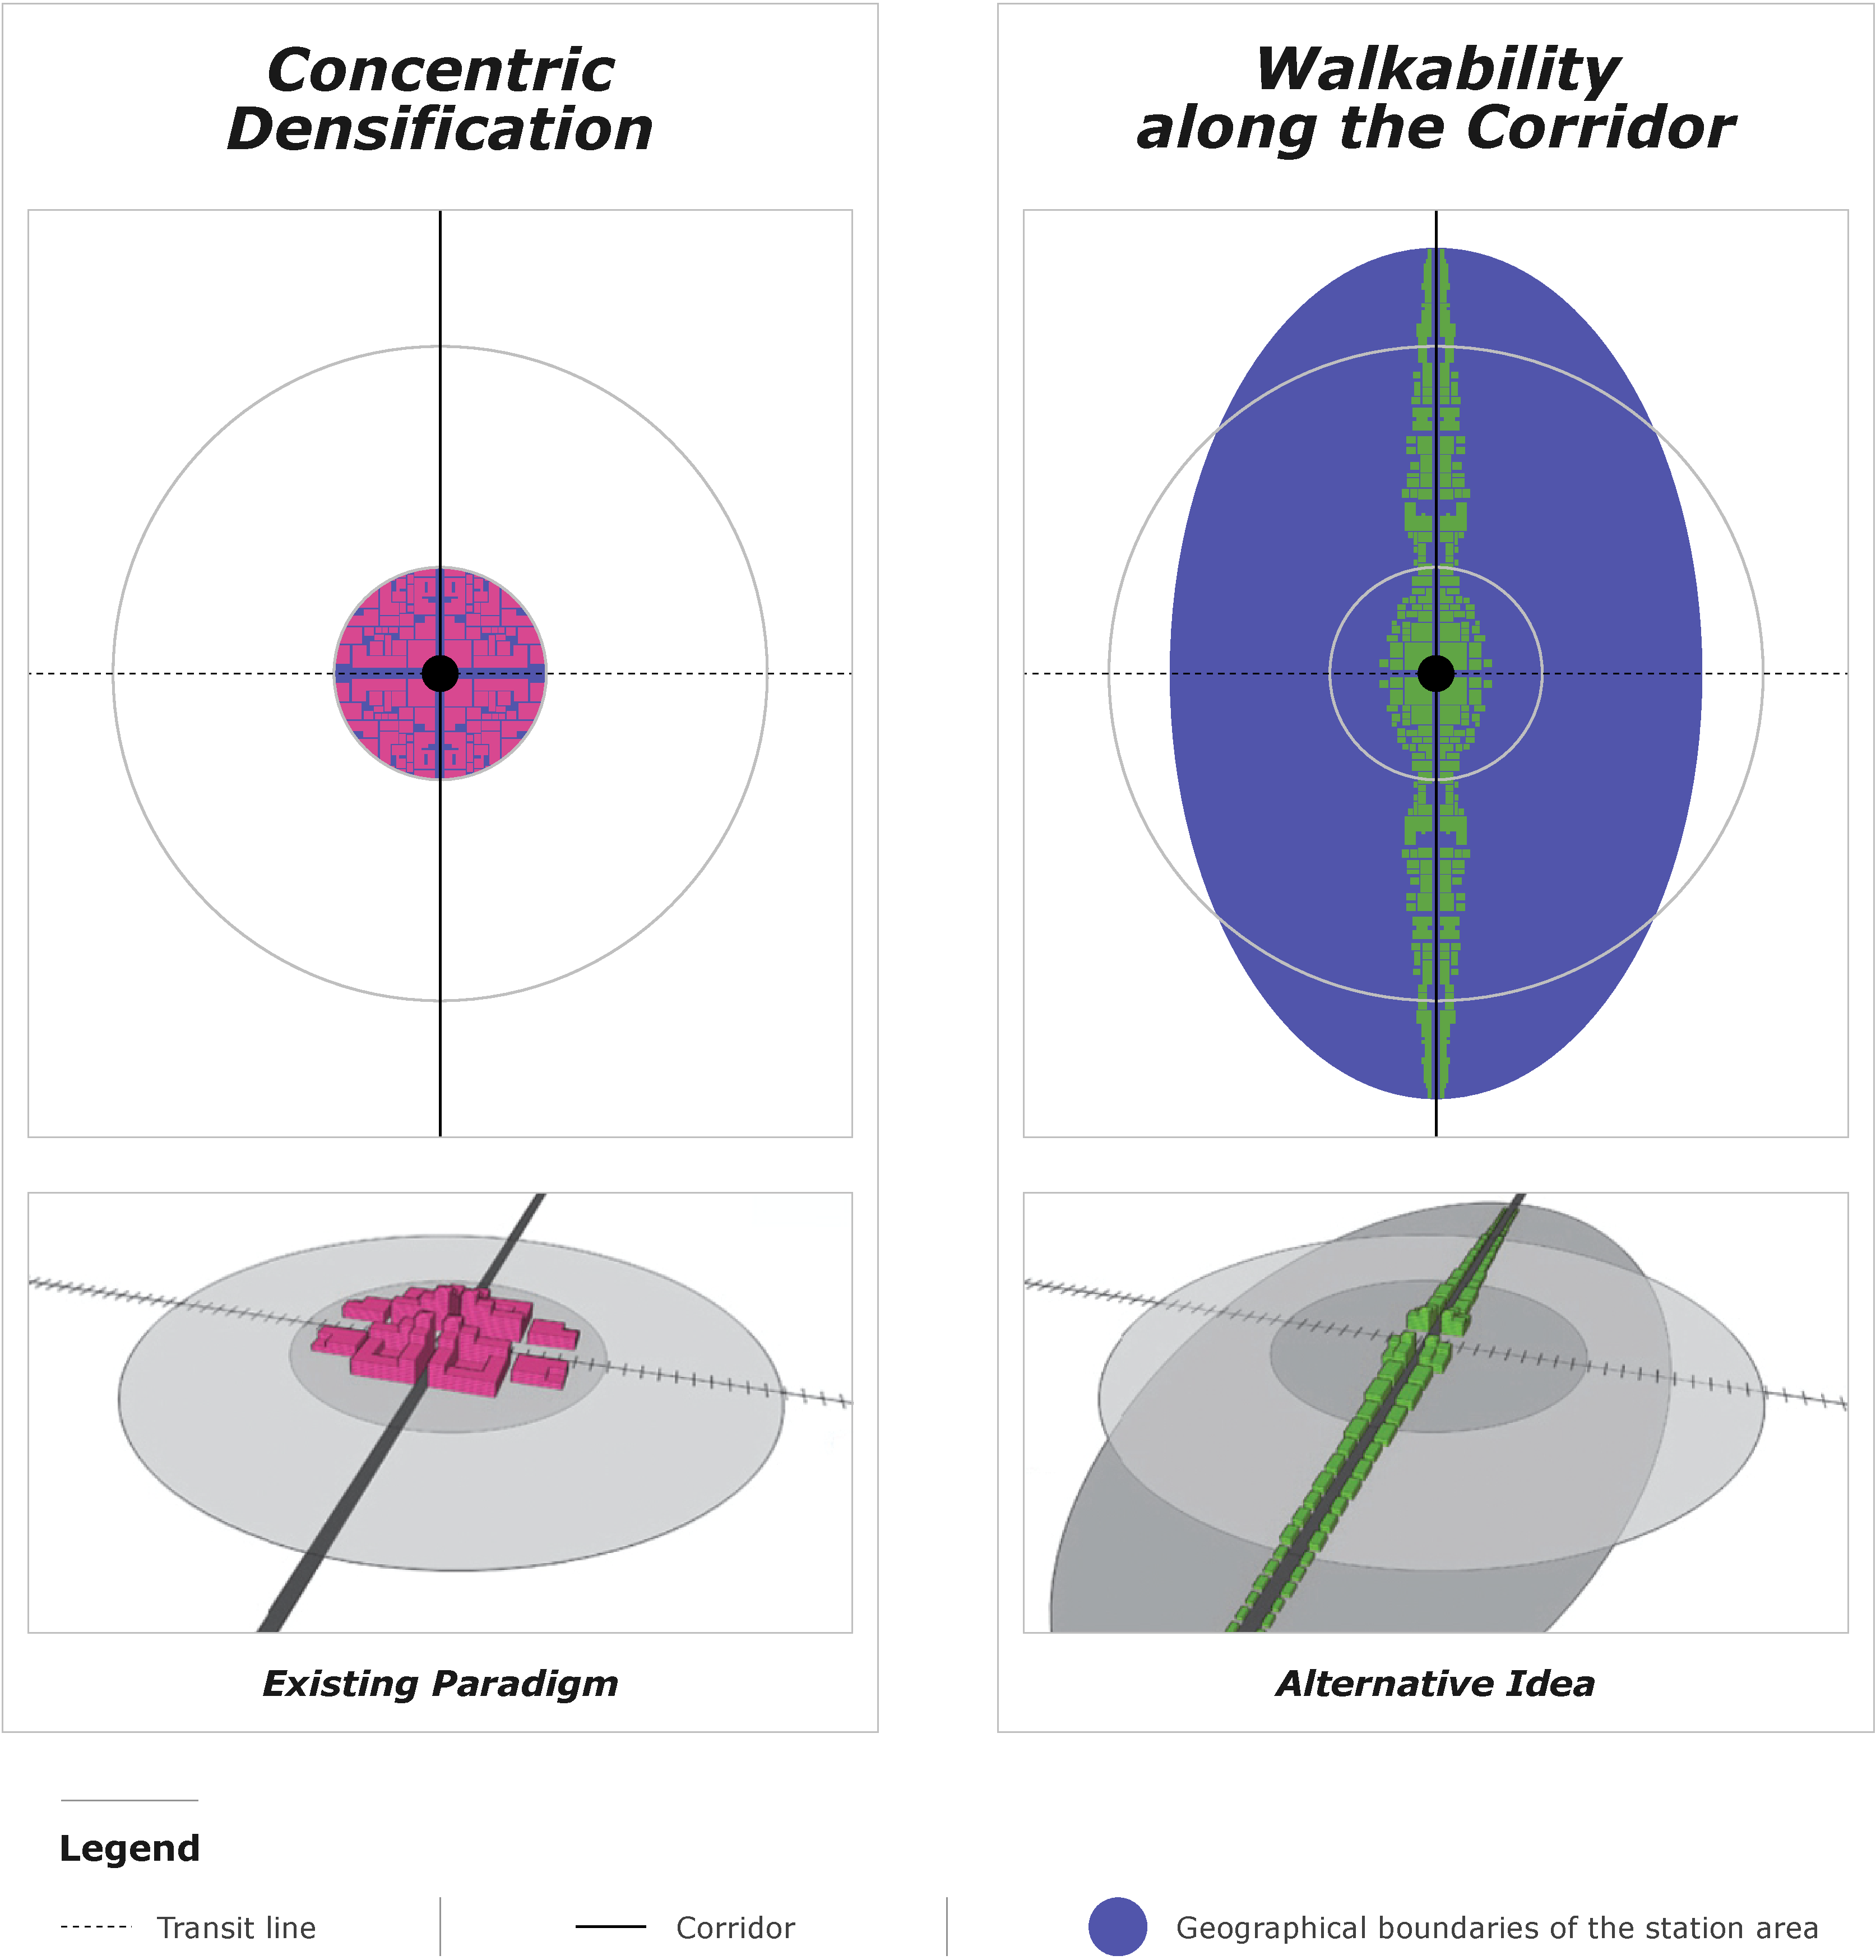
\includegraphics[width=1\columnwidth]{src/Figures/Chap-1/EN_Corridor_pieton.pdf}}
    \vspace{5pt}
    \begin{flushright}\scriptsize{
    Source: \textcolor{blue}{\textcite[163]{park_can_2015}}\index{Park, Sungjin|pagebf}\index{Deakin, Elizabeth|pagebf}\index{Jang, Kitae|pagebf}
    \\
    Graphic adaptation: \textcolor{blue}{Dylan Moinse (2025)}
    }\end{flushright}
\end{carte}

% Examples
Many studies today focus on the distance traveled by travelers to walk to or from a public transport station, generally supporting an underestimation of the pedestrian perimeters traditionally accepted around these nodes. On average, pedestrians accessing a train or metro station walk 1 kilometer, whether in San Francisco \textcolor{blue}{\autocite[5]{cervero_walk-and-ride_2001}}\index{Cervero, Robert|pagebf} or Singapore \textcolor{blue}{\autocite[41]{olszewski_using_2005}}\index{Olszewski, Piotr~S.|pagebf}\index{Wibowo, Sony Sulaksono|pagebf}. Using the 85\textsuperscript{th} percentile of the cumulative distance distribution, studies have shown that a distance of 1 kilometer (about 12 minutes walking) is considered acceptable around metro stations in Beijing \textcolor{blue}{\autocite[720]{yang_study_2013}}\index{Yang, Rongrong|pagebf}\index{Yan, Hai|pagebf}\index{Xiong, Wen|pagebf}\index{Liu, Tao|pagebf}, while slightly longer distances, 1.2 (for access) and 1.1 kilometers (for egress), are observed around train stations in Montreal \textcolor{blue}{\autocite[9]{el-geneidy_pedestrian_2009}}\index{El-Geneidy, Ahmed~M.|pagebf}\index{Tétreault, Paul|pagebf}\index{Surprenant-Legault, Julien|pagebf}. In the southeast of England, distances even reach 1.6 kilometers around stations \textcolor{blue}{\autocite[14]{bunn_how_2015}}\index{Bunn, Nick|pagebf}\index{Wakenshaw, Gareth|pagebf}. In the case of the Nord-Pas-de-Calais region, the 90\textsuperscript{th} percentile of rail passengers reveals that distances can reach 20 minutes on foot, compared to an observed average of 11 minutes \textcolor{blue}{\autocite[17]{hasiak_estimation_2018}}\index{Hasiak, Fabrice|pagebf}\index{Lannoy, Arnaud|pagebf}\index{Bodard, Géraldine|pagebf}\index{Palmier, Patrick|pagebf}. These variations reflect the major influence of certain urban environmental parameters, which can expand or contract these perceived distances \textcolor{blue}{\autocite[17]{soest_exploring_2020}}\index{Soest, Dennis van|pagebf}\index{Tight, Miles~R.|pagebf}\index{Rogers, Christopher~D.~F.|pagebf}. Already in 1984, \textcolor{blue}{Richard~k.} \textcolor{blue}{\textcite[23-59]{untermann_accommodating_1984}}\index{Untermann, Richard~K.|pagebf}, in his book \foreignlanguage{english}{\textsl{Accommodating the Pedestrian: Adapting Towns and Neighborhoods for Walking and Biking}}, showed that the maximum walking range in suburban areas, often confined to rigid thresholds of 400, 500, or 800 meters, could be considerably extended—even doubled—by designing attractive urban spaces and pleasant pedestrian corridors. More recent research confirms that urban diversity plays a key role. For example, a comparative study between Beijing, Tianjin, and Shenzhen indicates that pedestrians often double their walking distances when the urban environment features a high level of mixed-use, with shops and offices near transport stations \textcolor{blue}{\autocite[12]{zacharias_local_2017}}\index{Zacharias, John|pagebf}\index{Zhao, Qi|pagebf}. Similarly, in Australia and the United States, travelers are willing to walk an additional 800 meters when the urban environment follows the principles of \acrshort{TOD} \textcolor{blue}{\autocite[33]{canepa_bursting_2007}}\index{Canepa, Brian|pagebf}. Improving \Commas{micro-walkability} elements, particularly by strategically designing pedestrian corridors, appears to be a key lever to extend these spatial perimeters. Thus, \textcolor{blue}{\textcite[163]{park_can_2015}}\index{Park, Sungjin|pagebf}\index{Deakin, Elizabeth|pagebf}\index{Jang, Kitae|pagebf} demonstrate that it is possible to encourage public transport users to walk much greater distances by improving pedestrian infrastructure (see \hyperref[fig-chap1:tod-corridor-pieton]{Map~\ref{fig-chap1:tod-corridor-pieton}}, page~\pageref{fig-chap1:tod-corridor-pieton}). For example, creating pedestrian streets around stations increases the acceptable walking range to stations by 20\% in the United States, and by up to 120\% in Germany \textcolor{blue}{\autocite[151]{zielstra_comparative_2011}}\index{Zielstra, Dennis|pagebf}\index{Hochmair, Hartwig~H.|pagebf}.%%Translated%%

% Conclusion + Transition
Whether it's a pedestrian access area, represented as an Euclidean extent (circle) or calculated based on the road network (isodistance or isochrone), the arbitrary rule of 800 meters or 10 minutes of walking is more of a historical artifact than an analytical and statistical construction \textcolor{blue}{\autocite[102]{guerra_half-mile_2012}}\index{Guerra, Erick|pagebf}\index{Cervero, Robert|pagebf}\index{Tischler, Daniel|pagebf}. This rule, while commonly used, demonstrates its limitations. Indeed, while the primary service area perimeter of public transport stations, estimated at 800 meters, is not fundamentally incorrect—average distances for intercity rail often reaching 1,000 meters—the real difference lies in the method of measurement. By adopting an approach based on \Commas{acceptable} distance (considering the 85\textsuperscript{th} or 90\textsuperscript{th} percentiles) rather than just observable distance, it becomes clear that traditional pedestrian perimeters underestimate the actual distances traveled and experienced by users. For example, one study shows that traditional thresholds of 400 and 800 meters underestimate by 30\% the actual coverage of public transport accessible by foot in the Montreal region \textcolor{blue}{\autocite[20]{el-geneidy_new_2014}}\index{El-Geneidy, Ahmed~M.|pagebf}\index{Grimsrud, Michael|pagebf}\index{Wasfi, Rania|pagebf}\index{Tétreault, Paul|pagebf}\index{Surprenant-Legault, Julien|pagebf}. This highlights the need to move beyond the classical conception of walking. In France, while the average duration of pedestrian trips is 13 minutes, it is important to differentiate between monomodal walking and combined walking, used as a mode of connection to public transport stations. Indeed, while four out of five pedestrian trips in France last less than 15 minutes, those associated with combined walking frequently reach 20 minutes around train stations \textcolor{blue}{\autocite[23]{solere_mobilite_2010}}\index{Solere, Régis de|pagebf}\index{Papon, Francis|pagebf}. This increased range of combined walking is increasingly recognized in academic research, which considers it extendable depending on factors that enhance the \acrshort{TOD} potential of territories, such as urban density, functional mix, or the quality of pedestrian infrastructure. However, in peripheral neighborhoods, where the distances required to access public transport are much greater, walking alone is insufficient to correct these imbalances \textcolor{blue}{\autocite[85]{cervero_bike-and-ride_2013}}\index{Cervero, Robert|pagebf}\index{Caldwell, Benjamin|pagebf}\index{Cuellar, Jesus|pagebf}. To overcome the dichotomy between walking and public transport in central areas, and the car in intermodal areas in the suburbs, cycling can be the missing link in the intermodal chain. Yet, while academic and technical literature focuses almost exclusively on the accessibility of stations by foot, bike accessibility remains largely marginalized and under-studied \textcolor{blue}{\autocite[283]{martens_bicycle_2004}}\index{Martens, Karel|pagebf}. This gap represents a challenge to fully integrate cycling into accessibility and intermodality strategies, especially in areas where distances exceed the traditional capacities of walking.%%Translated%%

% 1.3.1.2.
\needspace{1\baselineskip} % Réserve de l'espace
\subsubsection*{Correcting the Weaknesses of Public Transport through an Intermodal Approach
    \label{chap1:btod-definition-intermodalite}
    }

    % Limitations of Walking
Given the limitations related to the reach of walking, which sometimes makes access to public transport stations restrictive, the effectiveness of \acrshort{TOD} is now being questioned. Indeed, the urban growth of territories has largely been based on distances adapted to the scale of the car, resulting in urban sprawl, often seen as a form of \Commas{suburbanization}. Furthermore, while public transport is effective in some respects, it lacks the flexibility advantages associated with the automobile \textcolor{blue}{\autocite[209]{heran_retour_2015}}\index{Héran, Frédéric|pagebf}. This situation calls into question the ability of the urban model to effectively combat dependence on motorized modes. Public transport represents only a partially adapted solution to reduce excessive reliance on the car. An alternative lies in the promotion of intermodality, which could address the rigidity of the public transport network \textcolor{blue}{\autocite[17]{wiel_comment_1998}}\index{Wiel, Marc|pagebf} and improve the overall efficiency of the mobility system \textcolor{blue}{\autocite[82]{oostendorp_combining_2018}}\index{Oostendorp, Rebekka|pagebf}\index{Gebhardt, Laura|pagebf}. Indeed, intermodality helps extend the influence area of nodes by integrating complementary solutions \textcolor{blue}{\autocite[16]{amar_homo_2016}}\index{Amar, Georges|pagebf}, which could strengthen their relevance in urban and suburban contexts marked by car dependency.%%Translated%%

% Intermodality
Interconnection refers to the link between two or more transport networks that are heterogeneous in their technical, organizational, and institutional dimensions, often associated with distinct mobility scales \textcolor{blue}{\autocites[]{dupuy_reseaux_1988}{varlet_interconnexion_1992}}\index{Dupuy, Gabriel|pagebf}\index{Varlet, Jean|pagebf}. The interest in this transition between different mobility regimes lies in the ability to go beyond the simple juxtaposition of unimodal networks that were not designed to be coordinated. This approach helps better understand the \Commas{concept-interface}, which relates multiple speeds of movement and spatial scales \textcolor{blue}{\autocite[156]{peters_time_1960}}\index{Peters, Peter Frank|pagebf}. This intermodal integration results in the formation of a meta-network, defined as a network of actual networks. It is a multiscalar nesting of systems that, through their interconnection, create an integrated megasystem \textcolor{blue}{\autocite[89]{ageron_intermodalite-voyageurs_2013}}\index{Ageron, Pierre|pagebf}\index{Varlet, Jean|pagebf}. Intermodal passenger mobility thus becomes a system-object, as a geographically located actor organization that generates places and practices \textcolor{blue}{\autocite[15]{varlet_interconnexion_1992}}\index{Varlet, Jean|pagebf}. Largely linked to public transport, intermodal passenger mobility is recognized as the most resource-efficient option in terms of travel time, cost, or energy consumption for making a trip from point A to point B \textcolor{blue}{\autocite[73]{oostendorp_combining_2018}}\index{Oostendorp, Rebekka|pagebf}\index{Gebhardt, Laura|pagebf}. In this sense, scheduling, interconnection, and intermodality of networks constitute efficiency factors that align with the principle of \Commas{reliance}. This principle, as a creator of links and synergies between varied flows, underpins new forms of network optimization \textcolor{blue}{\autocite[16-17]{amar_homo_2016}}\index{Amar, Georges|pagebf}. This evolution is accompanied by a growing modal diversification, driven by processes of (re)invention, technical and service innovation, as well as modal hybridization phenomena. These dynamics go beyond the binary vision of simply shifting from car use to public transport, promoting a multimodal and intermodal approach \textcolor{blue}{\autocite{richer_dossier_2021}}\index{Richer, Cyprien|pagebf}.%%Translated%%

% Figure functions and components of intermodality
\begin{figure}[h!]\vspace*{4pt}
    \caption{Functions and components of the intermodal system.}
    \label{fig-chap1:composantes-fonctions-intermodalite}
    \centerline{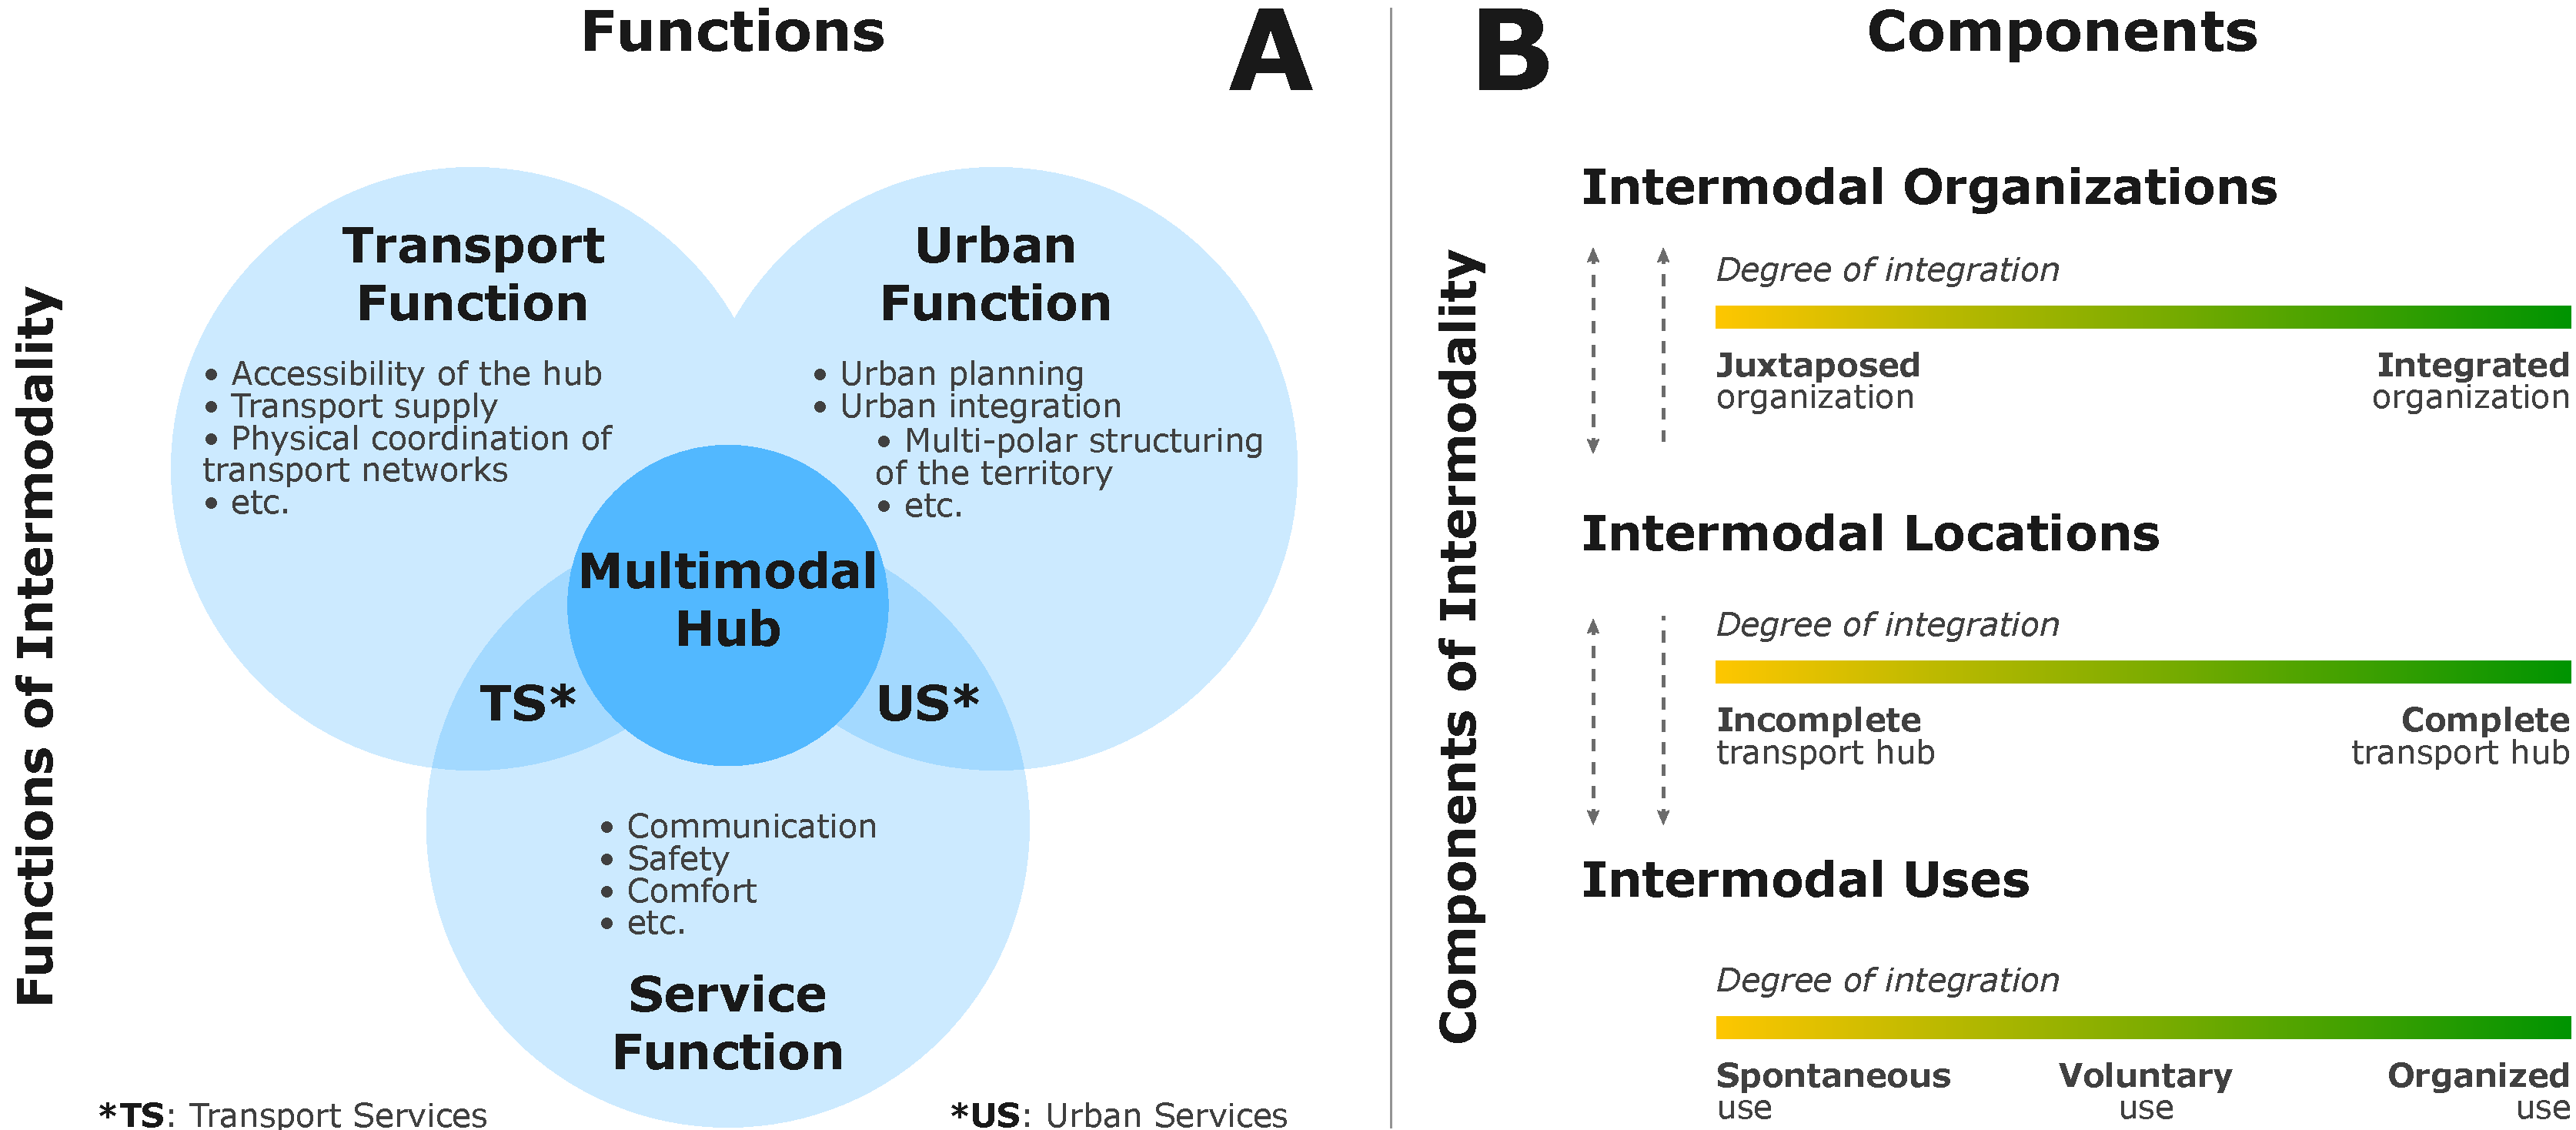
\includegraphics[width=1\columnwidth]{src/Figures/Chap-1/EN_Fonctions_Composants_Intermodalite.pdf}}
    \vspace{5pt}
    \begin{flushright}\scriptsize{
    Source (A): \textcolor{blue}{Cyprien} \textcolor{blue}{\textcite[14]{richer_lemergence_2008}}\index{Richer, Cyprien|pagebf}
    \\
    Source (B): \textcolor{blue}{Sandra} \textcolor{blue}{\textcite[167]{bozzani_grandes_2006}}\index{Bozzani-Franc, Sandra|pagebf}\index{Paris, Didier|pagebf}\index{Bakis, Henry|pagebf}\index{Menerault, Philippe|pagebf}
    \\
    Graphic adaptation: \textcolor{blue}{Dylan Moinse (2023)}
    }\end{flushright}
\end{figure}

% Intermodal System
The notion of intermodal passenger mobility can be analyzed through three main components proposed by \textcolor{blue}{Sandra} \textcolor{blue}{\textcite[167]{bozzani_grandes_2006}}\index{Bozzani-Franc, Sandra|pagebf}\index{Paris, Didier|pagebf}\index{Bakis, Henry|pagebf}\index{Menerault, Philippe|pagebf} in her doctoral thesis on the contribution of high-speed aero-rail intermodality (see \hyperref[fig-chap1:composantes-fonctions-intermodalite]{Figure~\ref{fig-chap1:composantes-fonctions-intermodalite}}, page~\pageref{fig-chap1:composantes-fonctions-intermodalite}). This tripartite framework is based on the \textsl{existence of an intermodal organization}, the \textsl{location in an intermodal space}, and \textsl{specific intermodal uses}, each dimension interacting with the others. These three aspects allow for evaluating the degree of integration of interconnection hubs based on the quality of service provided\footnote{~
    The quality of service in intermodality is expressed through cooperation and complementarity between operators, the coordination of schedules, the availability of intermodal information, the pooling of ticket reservations, a facilitated connection between modes, optimized connection and waiting times, and luggage handling \textcolor{blue}{\autocites[65]{bozzani_intermodalite_2005}[167]{bozzani_grandes_2006}}\index{Bozzani-Franc, Sandra|pagebf}\index{Paris, Didier|pagebf}\index{Bakis, Henry|pagebf}\index{Menerault, Philippe|pagebf}.
} \textcolor{blue}{\autocites[65]{bozzani_intermodalite_2005}[167]{bozzani_grandes_2006}}\index{Bozzani-Franc, Sandra|pagebf}\index{Paris, Didier|pagebf}\index{Bakis, Henry|pagebf}\index{Menerault, Philippe|pagebf}. Intermodality, made up of these three interrelated subsystems, requires an organization, is located in a space, and is made of uses. It thus allows for addressing key concepts in social sciences, such as the individual, place, and the world, as explained by \textcolor{blue}{Pierre} \textcolor{blue}{\textcite[490]{ageron_intermodalite-voyageurs_2013}}\index{Ageron, Pierre|pagebf}\index{Varlet, Jean|pagebf}. These subsystems are based on the principle of transcalarities, that is, an articulation between different spatial scales, a prerequisite for the complementarity of modes of transportation. Indeed, an intermodal association would not be of interest to the user if the modes involved were redundant in terms of territorial service and therefore of possible destinations \textcolor{blue}{\autocite[45]{ageron_intermodalite-voyageurs_2013}}\index{Ageron, Pierre|pagebf}\index{Varlet, Jean|pagebf}. From this perspective, intermodality is not limited to a simple succession of modes during a trip. It becomes a true \Commas{territorial resource}, understood as a combination of \Commas{production factors} that facilitate the proximity of spatial actors, in accordance with the definition by \textcolor{blue}{\textcite[6]{gumuchian_ressource_2007}}\index{Gumuchian, Hervé|pagebf}\index{Pecqueur, Bernard|pagebf}. In this regard, \textcolor{blue}{Cyprien} \textcolor{blue}{\textcite[14]{richer_lemergence_2008}}\index{Richer, Cyprien|pagebf}, then a research officer in geography at \acrshort{Cerema}, emphasizes the three constitutive functions of exchange hubs (see \hyperref[fig-chap1:composantes-fonctions-intermodalite]{Figure~\ref{fig-chap1:composantes-fonctions-intermodalite}}, page~\pageref{fig-chap1:tad-murdoch}): the \textsl{transport function}, the \textsl{urban function}, and the \textsl{service function}. These functions ensure not only the interconnection of networks but also the structuring of territories. The experiences with \textsl{Mobility Hubs}, conceptualized as part of the Interreg \textsl{Mobi-Mix} project, provide an illustration. They constitute points of intermodal facilitation, designed as physical hubs integrating at least two shared mobility systems, as evidenced in pilot projects in Norfolk and Valenciennes \textcolor{blue}{\autocites[3498]{hachette_exploring_2023}[248]{hachette_mobility_2023}}\index{Hachette, Maxime|pagebf}\index{L'Hostis, Alain|pagebf}\index{Gragera, Albert|pagebf}.%%Translated%%

% Relevance of MIL + Transition
According to \textcolor{blue}{\textcite[116]{goletz_intermodality_2020}}\index{Goletz, Mirko|pagebf}\index{Haustein, Sonja|pagebf}\index{Wolking, Christina|pagebf}\index{L'Hostis, Alain|pagebf}, strategic considerations on intermodality are increasingly prominent in the spatial planning directions. This trend reflects a promise of reducing car traffic, limiting car ownership, and acting as a catalyst for a genuine modal shift towards public transportation. Additionally, there is the idea that, in the future, new modes of transport that are still little used today will see an increase in their use and will significantly contribute to enriching intermodal chains. In this regard, \textcolor{blue}{\textcite[77]{oostendorp_combining_2018}}\index{Oostendorp, Rebekka|pagebf}\index{Gebhardt, Laura|pagebf} predict that the emergence of new forms of mobility, such as light individual mobility, will make intermodality even more relevant in the years to come. Integrating these \Commas{micro-modes} into public transport systems could provide many \Commas{co-benefits}, such as economic opportunities, health benefits, better inclusivity, cost savings for users, reductions in accidents and road congestion, as well as improvements in comfort and personal well-being \textcolor{blue}{\autocite[39-40]{litman_new_2021}}\index{Litman, Todd|pagebf}. In this context, light individual mobility positions itself as a family of modes complementary to public transport, similar to combined walking. It is likely to bring greater resilience to public transport systems \textcolor{blue}{\autocites{heran_velo_2020}[6]{dezobry_du_2020}}\index{Héran, Frédéric|pagebf}\index{Dezobry, Guillaume|pagebf}\index{Fontenelle, Louis de|pagebf}\index{Staropoli, Carine|pagebf}.%%Translated%%

% 1.3.2.
\needspace{1\baselineskip} % Reserve space
\subsection{From a \Commas{Station-to-Station} Approach to a \Commas{Door-to-Door} Approach
    \label{chap1:btod-definition}
    }

% Introduction
Categories of mobility that have long been considered antagonistic, such as individual transport and public transport, are gradually evolving towards a logic of \Commas{transmodality}. The emergence of intermodal configurations, made possible by the diversification of light individual mobility, thus promotes the affirmation of \Commas{individual public transport} \textcolor{blue}{\autocites[14-15]{amar_homo_2016}[18]{fijalkow_sociologie_2017}[5]{kostrzewska_towards_2017}}\index{Amar, Georges|pagebf}\index{Kostrzewska, Małgorzata|pagebf}\index{Macikowski, Bartosz|pagebf}\index{Fijalkow, Yankel|pagebf}. These compact vehicles provide an intelligent response to the challenges of the \Commas{first and last miles}, offering a \Commas{door-to-door} mobility solution that was long lacking in public transport \textcolor{blue}{\autocite{dia_banning_2019}}\index{Dia, Hussein|pagebf}. Integrated into an intermodal approach, light individual mobility is not limited to its technical specifics or its mode of acquisition: it generates unique travel practices that contribute to transforming mobility usage \textcolor{blue}{\autocite[1]{tuncer_notes_2020}}\index{Tuncer, Sylvaine|pagebf}\index{Laurier, Eric|pagebf}\index{Brown, Barry|pagebf}\index{Licoppe, Christian|pagebf}. Its potential lies notably in its ability to address the service gaps in public transport \textcolor{blue}{\autocites{gauquelin_case_2021}[3]{lee_forecasting_2021}}\index{Gauquelin, Alexandre|pagebf}\index{Lee, Mina|pagebf}\index{Chow, Joseph|pagebf}\index{Yoon, Gyugeun|pagebf}\index{He, Brian|pagebf}. By extending the influence zones of public transport stops, cycling has progressively been integrated into the reflection on \acrshort{TOD}, in the form of a \acrfull{B-TOD}, although it already played a strategic role in the \Commas{secondary areas}. From this point, the central question that emerges from this bibliographic work concerns the updating of this urban model and the added value represented by the integration of micromobility, as well as the diversification of cycling, in this renewal dynamic of \acrshort{TOD}.%%Translated%%

% 1.3.2.1.
\needspace{1\baselineskip} % Reserve space
\subsubsection*{Advantages of Integrating Light Individual Mobility
    \label{chap1:avantages-mil-tc}
    }

% Bicycle advantages
While the modal combination of cycling and public transport has garnered increasing interest and is expected to see a significant rise in usage by 2030 \textcolor{blue}{\autocite[119]{goletz_intermodality_2020}}\index{Goletz, Mirko|pagebf}\index{Haustein, Sonja|pagebf}\index{Wolking, Christina|pagebf}\index{L'Hostis, Alain|pagebf}, it is important to examine the comparative advantages that explain its attractiveness. First, from the perspective of speed, cycling allows for covering a spatial distance three to five times greater than walking, with an energy expenditure about five times lower \textcolor{blue}{\autocite[50]{sebban_complementarite_2003}}\index{Sebban, Annie-Claude|pagebf}\index{Motte, Alain|pagebf}. This increased speed significantly extends its range, and consequently, the relevant area of public transport stations. Indeed, for trips to and from a station, the acceptable distance is estimated to be 4 kilometers according to Dutch researcher \textcolor{blue}{Niels van} \textcolor{blue}{\textcite[4]{oort_overview_2020}}\index{Oort, Niels van|pagebf}, and even 5 kilometers according to a report from the European project \textcolor{blue}{\textcite[4]{bitibi_bike_2017}}\index{BiTiBi@\textsl{BiTiBi}|pagebf}. Taking the combined walking reach of 1 kilometer as a reference, extending this accessibility by bike would expand the influence area of a station by a factor of 25. Therefore, the challenge is to make neighborhoods that would not be considered \Commas{comfortably walkable} accessible via the combination of cycling and public transport \textcolor{blue}{\autocite[17]{nlc_micromobility_2019}}\index{NLC@\textsl{NLC}|pagebf}, especially in suburban areas where the car is a factor of exclusion for individuals without a driver's license or a motor vehicle \textcolor{blue}{\autocite[85]{cervero_bike-and-ride_2013}}\index{Cervero, Robert|pagebf}\index{Caldwell, Benjamin|pagebf}\index{Cuellar, Jesus|pagebf}. Another fundamental advantage lies in the ability of cycling to combine the spatial and temporal flexibility of a \Commas{door-to-door} mode with the extended reach and speed offered by public transport \textcolor{blue}{\autocite[212]{kager_characterisation_2016}}\index{Kager, Roland|pagebf}\index{Bertolini, Luca|pagebf}\index{te Brömmelstroet, Marco|pagebf}. Integrating cycling into the public transport network, as an alternative and decarbonized intermodal solution, allows for extending the service area of stations while being cost-effective both in terms of energy and budget. It thus promotes a form of socio-spatial justice by expanding accessibility to public transport for a larger number of potential users \textcolor{blue}{\autocite[99-100]{levine_mobility_2019}}\index{Levine, Jonathan|pagebf}\index{Grengs, Joe|pagebf}\index{Merlin, Louis~A.|pagebf}. These synergetic effects have been illustrated by \textcolor{blue}{\textcite[212]{kager_characterisation_2016}}\index{Kager, Roland|pagebf}\index{Bertolini, Luca|pagebf}\index{te Brömmelstroet, Marco|pagebf}, who graphically represent how the combination of cycling and public transport makes them more competitive than the car in terms of speed, flexibility, and range (see \hyperref[fig-chap1:vitesse-accessibilite-velo-tc]{Figure~\ref{fig-chap1:vitesse-accessibilite-velo-tc}}, page~\pageref{fig-chap1:vitesse-accessibilite-velo-tc}). This dynamic is particularly visible in urban congestion, and recalls the comparative advantages offered by carpooling.%%Translated%%

% Figure vitesse-accessibilité MIL+TC
\begin{figure}[h!]\vspace*{4pt}
    \caption{Characterization of the combination between light individual mobility according to the accessibility levels and speed of each mode of transport.}
    \label{fig-chap1:vitesse-accessibilite-velo-tc}
    \centerline{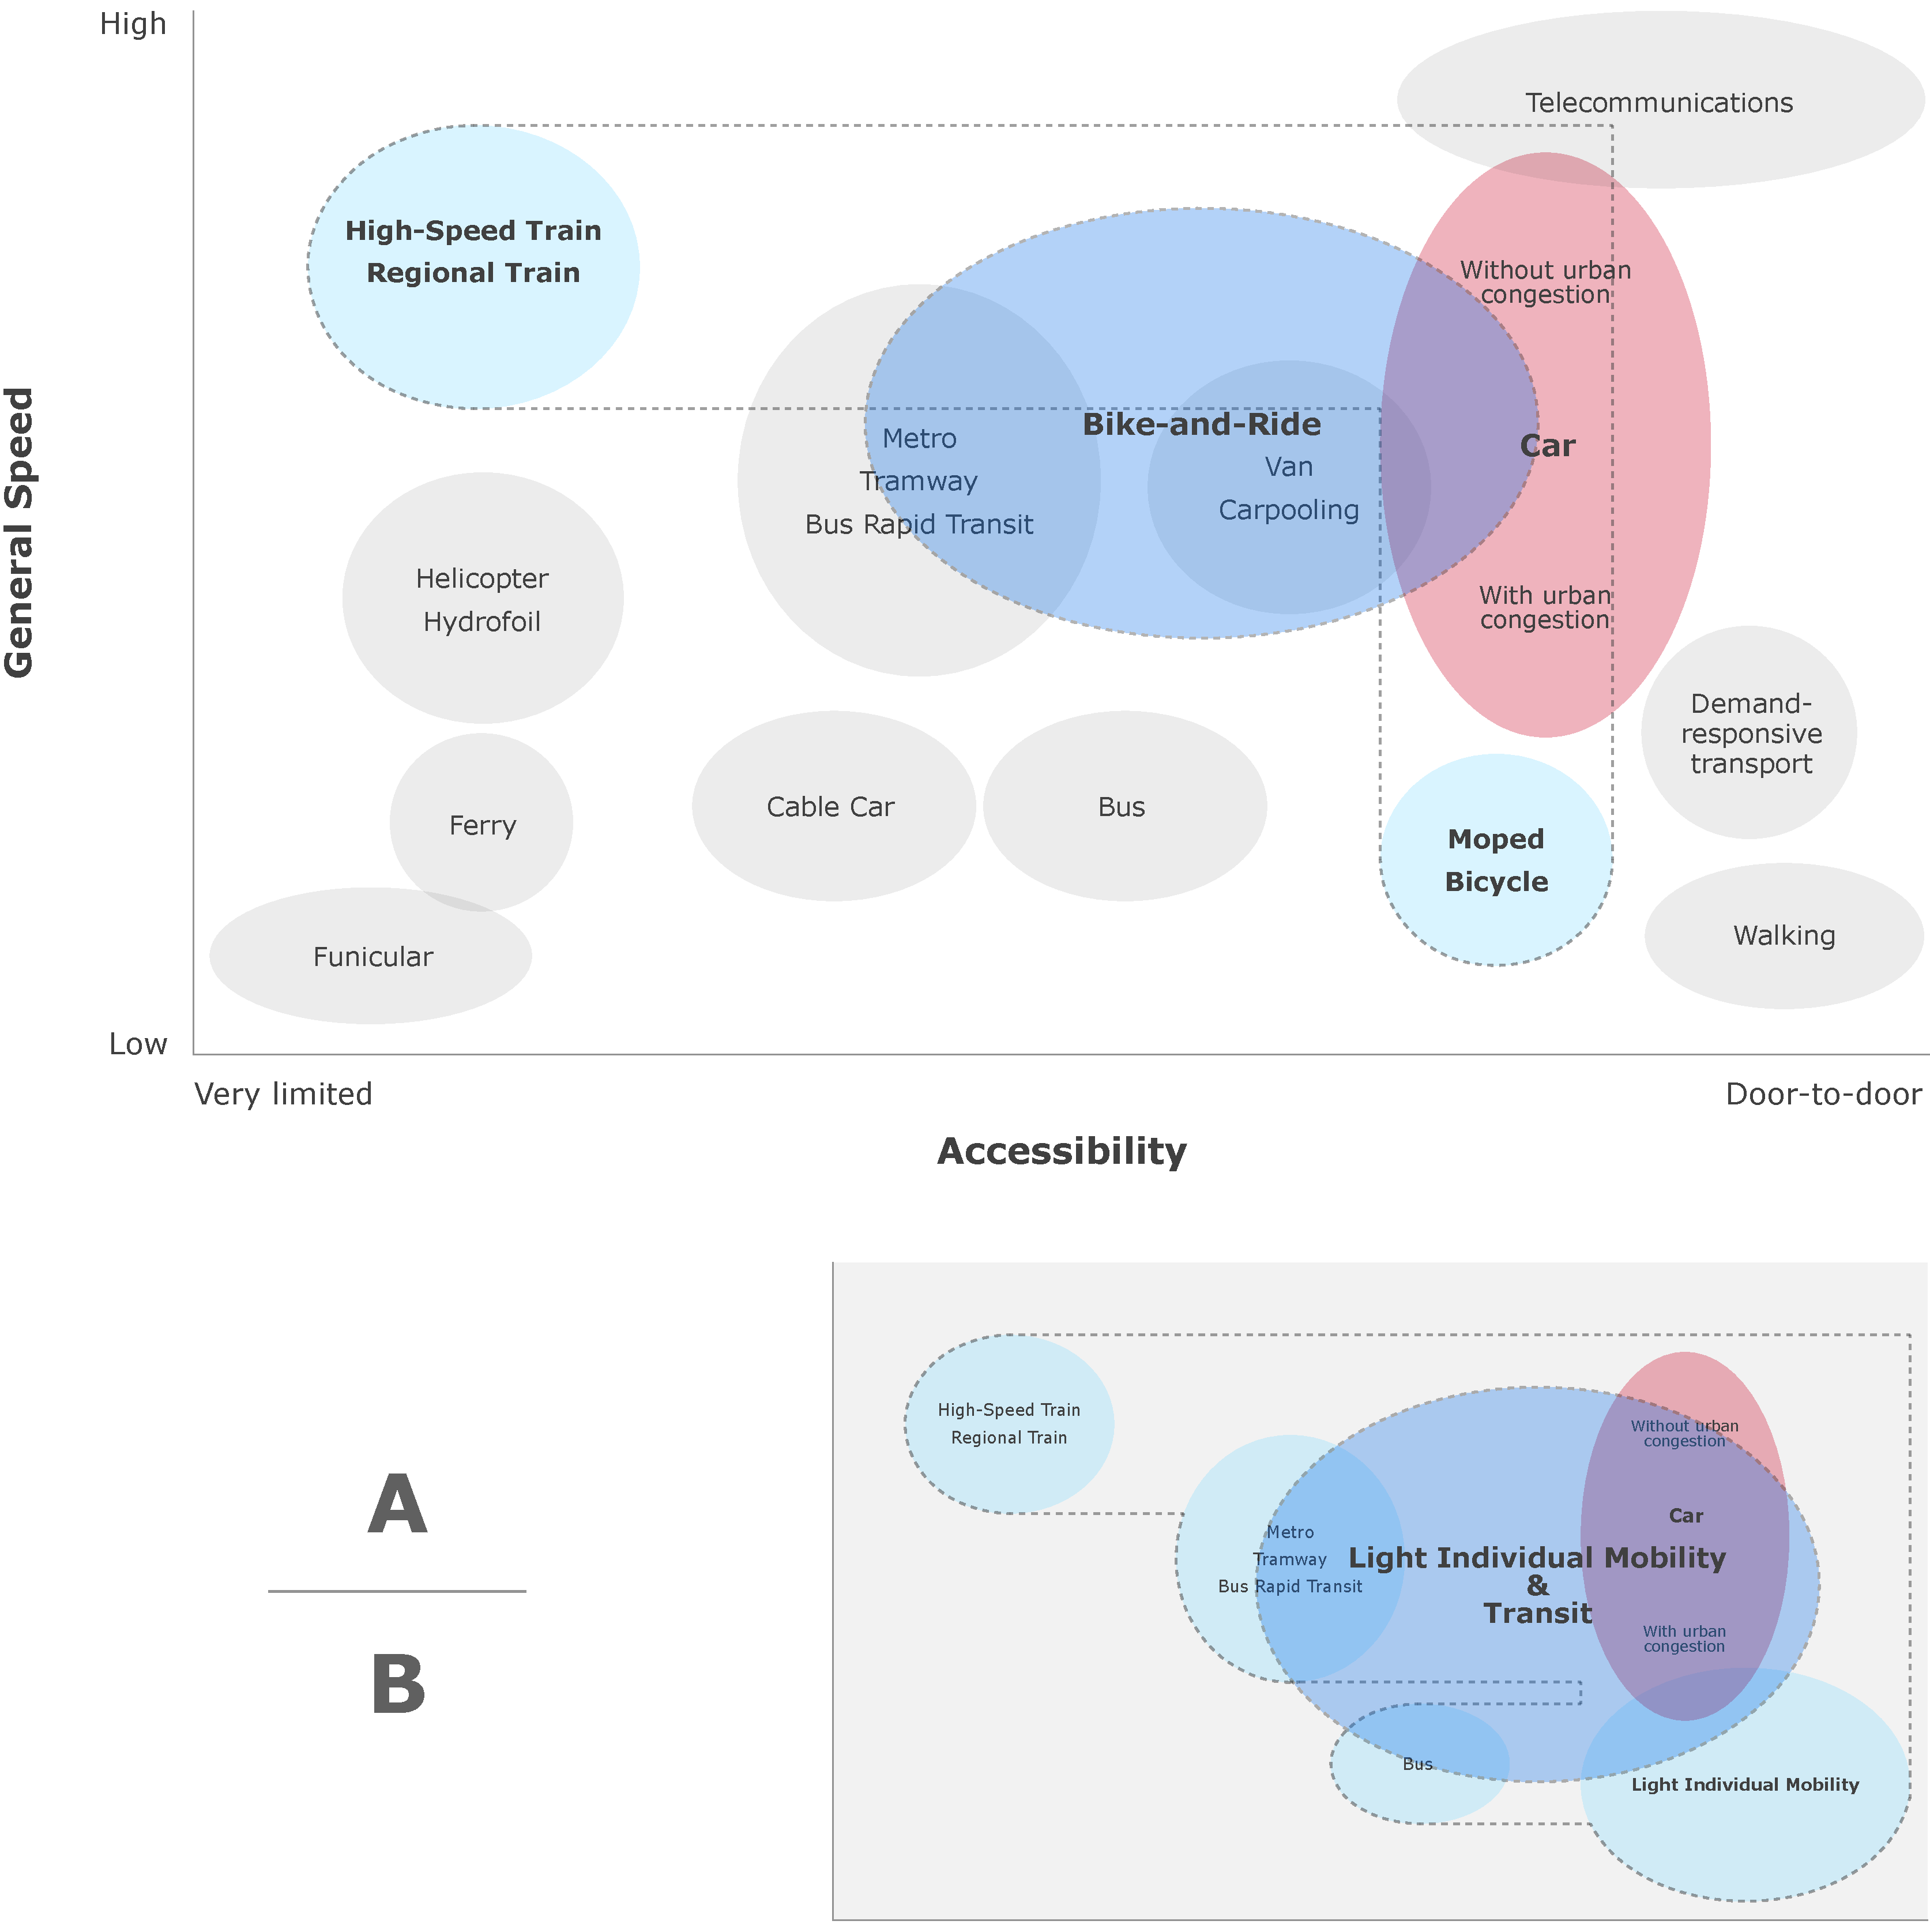
\includegraphics[width=1\columnwidth]{src/Figures/Chap-1/EN_Kager_vitesse_accessibilite.pdf}}
    \vspace{5pt}
    \begin{flushright}\scriptsize{
    Source (A): \textcolor{blue}{\textcite[212]{kager_characterisation_2016}}\index{Kager, Roland|pagebf}\index{Bertolini, Luca|pagebf}\index{te Brömmelstroet, Marco|pagebf}
    \\
    Graphic adaptation and reinterpretation (B): \textcolor{blue}{Dylan Moinse (2025)}
    }\end{flushright}
\end{figure}

% micromobility
While cycling is so well integrated into the \Commas{train system} in the Netherlands that a true bimodal mode of transport called \Commas{bike-train} has emerged \textcolor{blue}{\autocite[129-148]{bruntlett_curbing_2020}}\index{Bruntlett, Melissa|pagebf}\index{Bruntlett, Chris|pagebf}, \Commas{bike-train}, what about micromobility? It seems that this family of mobility devices serves a function and possesses properties similar to those of bicycles. Indeed, \acrshort{PMD}\textcolor{blue}{s} offer comparable potential for extending the reach of walking, allowing distances two to three times longer to be covered at a speed about three times higher \textcolor{blue}{\autocite{rabaud_micromobilites_2019}}\index{Rabaud, Mathieu|pagebf}\index{Richer, Cyprien|pagebf}. Thus, micromobility also contributes to redefining the catchment areas of public transport, facilitating access to stations and expanding their area of influence. A specific advantage of \acrshort{PMD}\textcolor{blue}{s}, however, lies in their compactness and lightness, which make them more easily carried on public transport, unlike traditional bicycles (see \hyperref[fig-chap1:vitesse-accessibilite-velo-tc]{Figure~\ref{fig-chap1:vitesse-accessibilite-velo-tc}}, page~\pageref{fig-chap1:vitesse-accessibilite-velo-tc}). Therefore, whether it’s a bicycle or micromobility devices, these modes meet similar needs and expectations: the pursuit of greater flexibility and direct, more flexible access to nodes that align with environmental goals \textcolor{blue}{\autocite[80]{oostendorp_combining_2018}}\index{Oostendorp, Rebekka|pagebf}\index{Gebhardt, Laura|pagebf}.%%Translated%%

% Impacts + Transition
The benefits of the combination of light individual mobility and public transport, including the increased distances that users are willing to travel to access or leave a public transport station, would contribute to a significant increase in the network's ridership \textcolor{blue}{\autocite[]{wang_approximating_2016}}\index{Wang, Hai|pagebf}\index{Odoni, Amedeo|pagebf}. A model developed by \textcolor{blue}{\textcite[69]{ensor_mode_2021}}\index{Ensor, Matt|pagebf}\index{Maxwell, O.|pagebf}\index{Bruce, Oliver|pagebf} shows that the rise of cycling and \acrshort{PeS} practices could lead to a 7\% increase in public transport ridership in urban areas, and a 9\% increase in suburban areas in New Zealand, if intermodal configurations are optimized. This finding highlights a key point: although cycling and micromobility cannot be fully competitive with the car over long distances and have limited capacity to replace it, their integration with public transport creates a synergy that makes them highly competitive against this mode of transport \textcolor{blue}{\autocite[43]{corporate_partnership_board_good_2020}}\index{Corporate Partnership Board@\textsl{Corporate Partnership Board}|pagebf}. As \textcolor{blue}{Annie-Claude} \textcolor{blue}{\textcite[262]{sebban_complementarite_2003}}\index{Sebban, Annie-Claude|pagebf}\index{Motte, Alain|pagebf} explains, the intermodality of cycling and public transport is structured around \textsl{practice territories}. This approach allows the concept of territory to be mobilized, as these intermodal practices operate \textsl{on} and \textsl{between} well-defined spaces. Considering intermodality from a territorial perspective naturally leads us back to the \acrshort{TOD} model. This framework appears to be a relevant one to revisit in light of the challenges related to the \Commas{first and last miles}, to which light individual mobility seems particularly suited.%%Translated%%

% 1.3.2.2.
\needspace{1\baselineskip} % Reserve space
\subsubsection*{Conceptualizing a Rail-Oriented Urbanism Supported by Light Individual Mobility
    \label{chap1:btod-m-tod}
    }

    % Introduction to secondary areas
In their work offering a contemporary view of \acrshort{TOD}, \foreignlanguage{english}{\textsl{Transit-Oriented Development and Sustainable Cities: Economics, Community and Methods}}, \textcolor{blue}{\textcite[222]{knowles_transit_2019}}\index{Knowles, Richard~D.|pagebf}\index{Ferbrache, Fiona|pagebf} emphasize the importance of leveraging opportunities provided by emerging mobilities in recent years—such as \acrshort{e-Bike}, \acrshort{PeS}, and dockless sharing services—in order to enrich the \acrshort{TOD} urban model. \textcolor{blue}{Peter} \textcolor{blue}{\textcite[54-55]{calthorpe_next_1993}}\index{Calthorpe, Peter|pagebf} does not disregard the importance of considering the \Commas{secondary areas} in the structuring of \acrshort{TOD} neighborhoods. He partially integrates them into \acrshort{TOD}, considering them sufficiently close to a public transport station to be oriented towards it, especially via a cycling connection. The \Commas{secondary area} even shares characteristics with the \Commas{primary area}, benefiting from some functional diversity and being connected to a network of calm streets. Far from being marginal, this area plays a structuring role in every train station district. It typically accommodates functions that are rarely configured to be placed in the most strategic area, such as jobs outside office spaces, schools, or parks. It also offers diversity in terms of housing choices, often including detached houses. The author identifies three types of \Commas{secondary areas}: (i) those separated by a road but close to a public transport stop; (ii) those separated by a road and distant from the stop; (iii) and those even farther from the stop but without a separating road \textcolor{blue}{\autocite[87]{calthorpe_next_1993}}\index{Calthorpe, Peter|pagebf}. Although the \Commas{secondary area} is often more car-oriented and frequently hosts infrastructure like \acrfull{PnR} encouraging the practice of park-and-ride, it should, according to him, be served by cycling connections directly linking it to the public transport station and the central train station district. From the moment \acrshort{TOD} is formalized, the major challenge lies in maximizing pedestrian and, especially, cycling connections within the \Commas{secondary area}. He specifically recommends the construction of separated bike lanes along major urban boulevards\footnote{~
    \Commas{\textsl{Due to the distances, bicycles are one of the most likely modes of travel for residents of secondary areas who are apt to use public transit. Strong bicycle connections following the shortest possible routes will provide additional encouragement for secondary area residents to use transit. Arterial roads and certain connecting routes in secondary areas must provide safe, separated or marked bicycle lanes allowing quick travel to the transit stop. Secondary area bicycle paths should connect to the TOD bicycle network.}} \textcolor{blue}{\autocite[89]{calthorpe_next_1993}}\index{Calthorpe, Peter|pagebf}.
} \textcolor{blue}{\autocite[60, 89]{calthorpe_next_1993}}\index{Calthorpe, Peter|pagebf}. In addition to these developments, the author emphasizes the importance of secure bike parking to encourage intermodal use, as well as the role of bicycles in internal mobility within the train station district\footnote{~
    \Commas{\textsl{Secure bike lockers are especially important for \Commas{bike-and-ride} transit use, as few will leave their bike unattended for a full working day. Bicycle parking facilities include bike racks, \Commas{checks,} and lockers. Bike racks must be provided at shopping, school, and recreational destinations in TODs and secondary areas. More secure bike parking facilities should be provided near all offices, workplaces, and major public transport stops.}} \textcolor{blue}{\autocite[103]{calthorpe_next_1993}}\index{Calthorpe, Peter|pagebf}.
} \textcolor{blue}{\autocite[103]{calthorpe_next_1993}}\index{Calthorpe, Peter|pagebf}. More than a simple connection to the main network, it is about offering a comprehensive cycling network that provides access to all amenities in the train station district—whether located in the primary or secondary area—and effectively linking one \acrshort{TOD} to another\footnote{~
    \Commas{\textsl{A coordinated system of bikeways should be provided in conjunction with TODs or a series of TODs. Important destinations, such as core commercial areas, transit stops, employment centers, parks, open spaces, schools, and other community facilities, should be linked by these bike routes.} [\dots] \textsl{Separated or marked bike lanes on several primary routes to the core area will support this alternative, as will the bike paths along greenways between TODs and employment destinations. On smaller streets, bikes sharing the travel lane will help slow cars to speeds more appropriate for residential streets. Selected routes to the transit stop should provide marked or separated bikeways connecting with the secondary areas and other key destinations. Designated bike lanes should be provided on selected connector streets and a limited number of local streets converging upon the commercial and transit center.} [\dots] \textsl{Clear destination signs should be provided that direct riders to key activity centers, such as shopping areas, transit stops, recreation facilities, schools, and bike parking facilities.}} \textcolor{blue}{\autocite[102]{calthorpe_next_1993}}\index{Calthorpe, Peter|pagebf}.
} \textcolor{blue}{\autocite[102]{calthorpe_next_1993}}\index{Calthorpe, Peter|pagebf}. Thus, considering the comparative advantages related to the integration of light individual mobility into the public transport network, the challenge goes beyond the simple \Commas{pedestrian pocket} to aim for a full integration of the \Commas{secondary area} within the \acrshort{TOD} \textcolor{blue}{\autocite[112]{ibraeva_transit-oriented_2020}}\index{Ibraeva, Anna|pagebf}\index{Almeida Correia, Gonçalo Homem de|pagebf}\index{Silva, Cecília|pagebf}.%%Translated%%

% Figure B-TOD
\begin{carte}[h!]\vspace*{4pt}
    \caption{Spatial configurations of the \textsl{Bicycle-based Transit-Oriented Development}.}
    \label{fig-chap1:schema-b-tod}
    \centerline{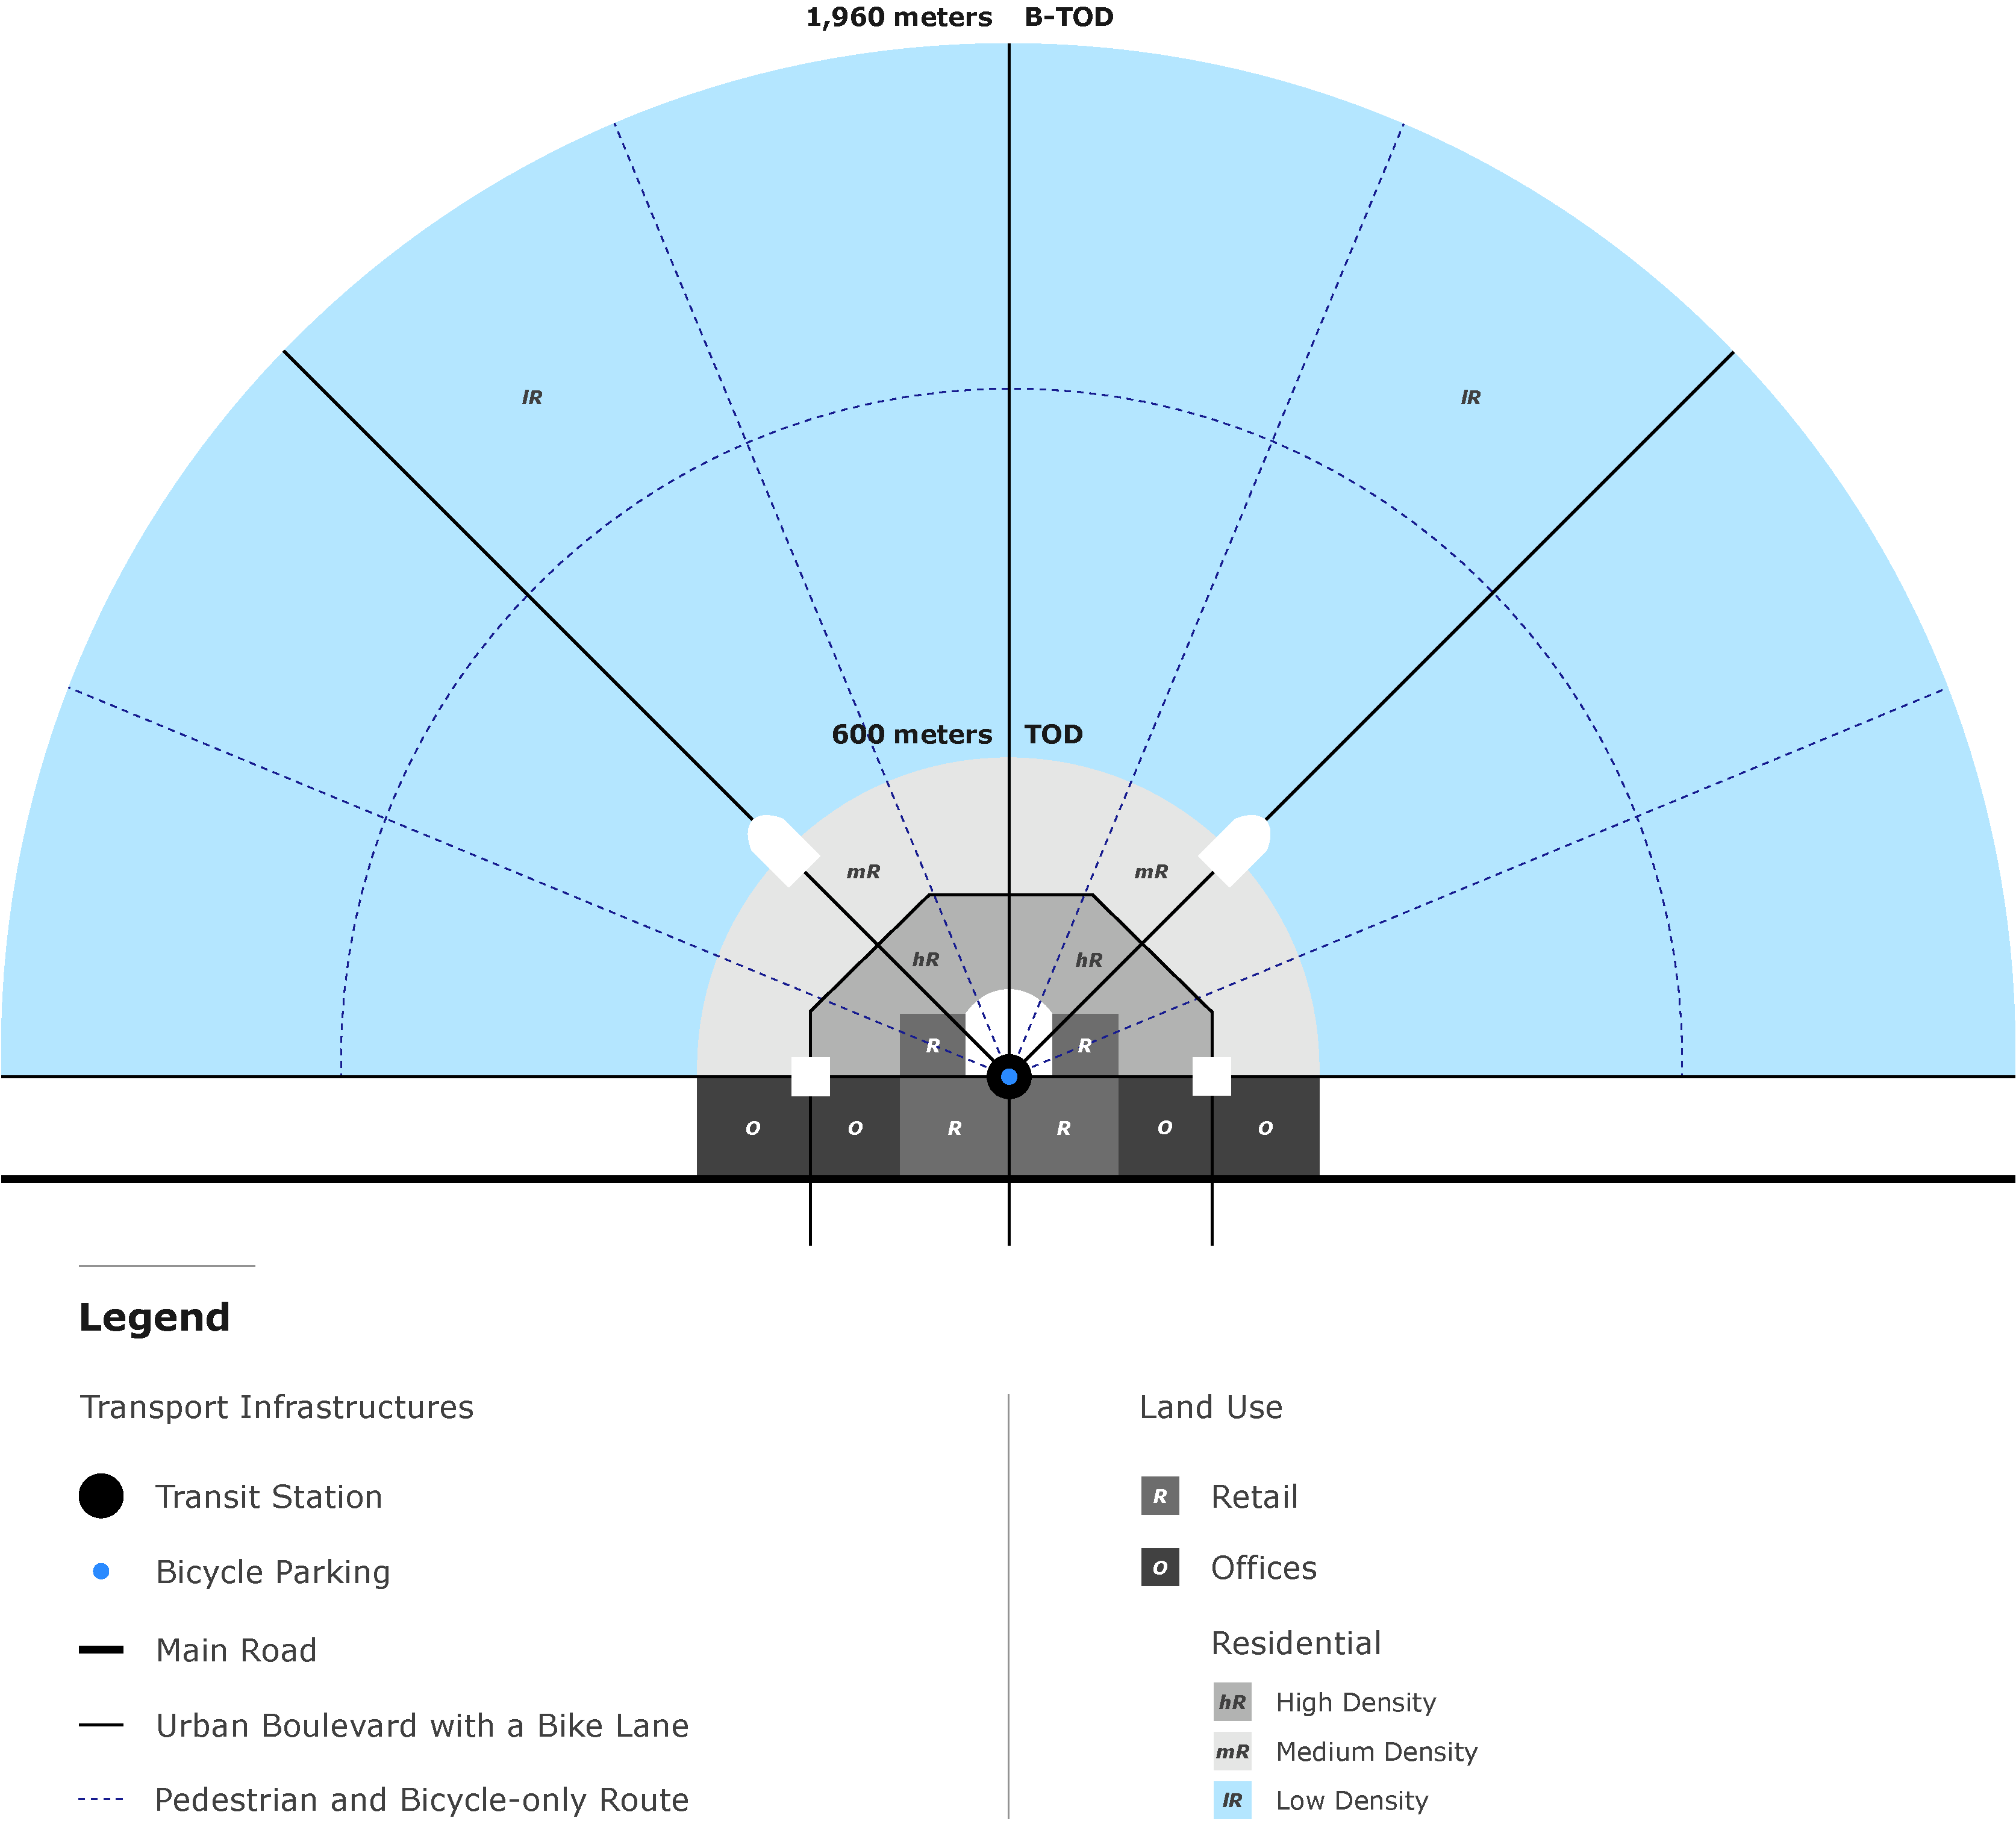
\includegraphics[width=1\columnwidth]{src/Figures/Chap-1/EN_Schema_B_TOD.pdf}}
    \vspace{5pt}
    \begin{flushright}\scriptsize{
    Source: \textcolor{blue}{\textcite[979]{lee_bicycle-based_2016}}\index{Lee, Jaeyeong|pagebf}\index{Choi, Keechoo|pagebf}\index{Leem, Yountaik|pagebf}
    \\
    Graphic adaptation: \textcolor{blue}{Dylan Moinse (2024)}
    }\end{flushright}
\end{carte}

% B-TOD
Although the issue of the \Commas{first and last miles} and the intermodal solution associated with cycling were considered as early as the foundational work of \acrshort{TOD}, it appears that the developments related to the \Commas{secondary area} and proposed cycling facilities have gradually lost visibility and clarity in the principles outlined. In response to this partial appropriation, South Korean researchers \textcolor{blue}{\textcite[979]{lee_bicycle-based_2016}}\index{Lee, Jaeyeong|pagebf}\index{Choi, Keechoo|pagebf}\index{Leem, Yountaik|pagebf}, in their article \textsl{Bicycle-based transit-oriented development as an alternative to overcome the criticisms of the conventional transit-oriented development}, propose, two decades later, the conceptualization of a \acrfull{B-TOD} (see \hyperref[fig-chap1:schema-b-tod]{Map~\ref{fig-chap1:schema-b-tod}}, page~\pageref{fig-chap1:schema-b-tod}). This variation of \acrshort{TOD}, which does not challenge the fundamental principles of the model, aims to address the needs of areas that have not reached the critical population and employment density thresholds necessary to maximize demand for transport around stations. The \acrshort{B-TOD} thus seeks to increase public transport network usage by targeting areas within a 2-kilometer radius accessible by bike \textcolor{blue}{\autocite[979]{lee_bicycle-based_2016}}\index{Lee, Jaeyeong|pagebf}\index{Choi, Keechoo|pagebf}\index{Leem, Yountaik|pagebf}. This revised model presents other notable advantages. It allows for an expansion of up to 25 times the area of a traditional train station district, thus significantly enhancing its attractiveness potential. Moreover, with easier implementation, it positions itself as an ecological alternative to the \acrshort{TOD} and \acrshort{E-TOD} models, requiring only a modest infrastructure investment \textcolor{blue}{\autocite[979, 983]{lee_bicycle-based_2016}}\index{Lee, Jaeyeong|pagebf}\index{Choi, Keechoo|pagebf}\index{Leem, Yountaik|pagebf}, as we discussed in the \hyperref[chap1:tod-presentation-generale-declinaisons-hybrids]{subsection on \textsl{Transit-Oriented Development} hybrids} (page~\pageref{chap1:tod-presentation-generale-declinaisons-hybrids}). A fourth advantage, less explicitly stated by the authors, is worth mentioning in our view: the \acrshort{B-TOD} could allow for an adaptation of the \Commas{[\dots] \textsl{population density criteria that would be more or less relaxed compared to those of the central area to maintain a more pleasant environment in this area.}}\footnote{~
    \Commas{\textsl{In a B-TOD setting, the re-establishment of the station impact area, where bicycle is a main access mode should be identified and the density criteria could be more or less relaxed than that of a TOD to keep the station impact area more pleasant.}} \textcolor{blue}{\autocite[983]{lee_bicycle-based_2016}}\index{Lee, Jaeyeong|pagebf}\index{Choi, Keechoo|pagebf}\index{Leem, Yountaik|pagebf}.
} \textcolor{blue}{\autocite[983]{lee_bicycle-based_2016}}\index{Lee, Jaeyeong|pagebf}\index{Choi, Keechoo|pagebf}\index{Leem, Yountaik|pagebf}. However, this does not mean reducing the density but rather better distributing it within the \acrshort{B-TOD} area by offering residential opportunities for individuals looking for less dense areas, better equipped with green spaces, offering easier access to family housing, or allowing escape from the land pressure surrounding centralities. To validate their conceptualization exercise, the authors conducted a survey with \Commas{intermodal cyclists}—this is the term we prefer to describe users combining cycling and public transport on the same trip—in the cities of Seoul and Daejeon. Their modeling shows that 94\% of the Seoul metropolitan area could be made accessible by public transport through intermodal cycling use, which is three times the coverage provided by combined walking \textcolor{blue}{\autocite[982]{lee_bicycle-based_2016}}\index{Lee, Jaeyeong|pagebf}\index{Choi, Keechoo|pagebf}\index{Leem, Yountaik|pagebf}. Reorganizing urbanism around public transport and bicycles not only promotes ecology but also health and physical activity \textcolor{blue}{\autocite[44]{heran_velo_2020}}\index{Héran, Frédéric|pagebf}\index{Rymarski, Christophe|pagebf}\index{Bedin, Véronique|pagebf}, a dimension less addressed in conventional \acrshort{TOD}.%%Translated%%

% M-TOD
Building on this variation, we have chosen to rely on this foundational research work, which seems to be the cornerstone, in order to draw inspiration from it and transpose our argument developed throughout this chapter. Specifically, it aims to demonstrate the potential of light individual mobility to strengthen the urban model of \acrshort{TOD}, with a view to promoting more sustainable mobility and urban environments. Drawing inspiration from the arguments put forward by \textcolor{blue}{\textcite{lee_bicycle-based_2016}}\index{Lee, Jaeyeong|pagebf}\index{Choi, Keechoo|pagebf}\index{Leem, Yountaik|pagebf}, and particularly revisiting their questions regarding the \Commas{identification} and \Commas{definition} of a \acrshort{B-TOD}, we propose an update of these models to design an \acrfull{M-TOD}. Ultimately, we could transpose the proposal for a \Commas{general theory of walkability} formulated by urban planner \textcolor{blue}{Jeff} \textcolor{blue}{\textcite[73]{speck_walkable_2013}}\index{Speck, Jeff|pagebf} into a \Commas{general theory of bikeability} articulated around the public transport system. This would integrate all light individual mobility and fulfill, just like walkability, a threefold function: that of a purpose in itself, a means of accessibility, and a measure of urban quality \textcolor{blue}{\autocite[73]{speck_walkable_2013}}\index{Speck, Jeff|pagebf}. Thus, several questions structure, at this stage, our reflection:
\begin{customitemize}
\item What is an \acrshort{M-TOD} and how does it differ from a \acrshort{TOD} and a \acrshort{B-TOD}?
\item What are its observable uses and what is its modal shift potential?
\item What are the connections between public transport and light individual mobility?
\item How do these current and potential mobility behaviors interact with the urban fabric and territorial development challenges?
\end{customitemize}%%Translated%%

% ___________________________________________
% 1.*.
\newpage
\needspace{1\baselineskip} % Reserve space
\addcontentsline{toc}{section}{Conclusion of Chapter~1}
\sectionheader{Conclusion of Chapter~1}
\section*{Conclusion of Chapter~1
    \label{chap1:conclusion}
    }
    \markright{Conclusion of Chapter~1}{}

    % Introduction
The \acrfull{TOD} now constitutes a strategic lever for sustainable urban planning, offering a response to the challenges posed by the \Commas{car everywhere} and \Commas{car above all} policies, which continue to guide urban development in France \textcolor{blue}{\autocite[14]{sebban_complementarite_2003}}\index{Sebban, Annie-Claude|pagebf}\index{Motte, Alain|pagebf}. This chapter has revisited the historical foundations, guiding principles, and contemporary variations of this urban planning model. Although its formalization emerged in the North American context, it would be wrong to attribute its creation exclusively to American urban planners, as they themselves acknowledged drawing inspiration from European examples \textcolor{blue}{\autocite[15]{renne_emerging_2004}}\index{Renne, John Luciano|pagebf}\index{Wells, J.~S.|pagebf}. In sum, the theoretical and operational framework of \acrshort{TOD} provides a solid and relevant foundation for addressing current environmental and socio-economic imperatives, both at the regional and local levels. It is not only about promoting a better public transport offer—although this is a necessary condition—but about integrating this offer within an interaction with territorial structuring \textcolor{blue}{\autocite[9]{bernier_atlas_2023}}\index{Bernier, Xavier|pagebf}, following a dynamic of \Commas{congruence}\footnote{~
    In his article titled \textsl{The \Commas{structural effects} of transport: political myth, scientific mystification}, \textcolor{blue}{Jean-Marc} \textcolor{blue}{\textcite[239]{offner__1993}}\index{Offner, Jean-Marc|pagebf} notably exposed the need for a \Commas{demystification} of the political-media and scientific discourse concerning the evaluation and expectations surrounding the \Commas{structural effects} of transport infrastructure. He challenges the idea of a linear causal relationship between the introduction of new mobility offerings and territorial development, highlighting a more complex pre-existing dynamic of parallel connections, which he terms \Commas{congruence}.
}, a concept developed by \textcolor{blue}{Jean-Marc} \textcolor{blue}{\textcite[239]{offner__1993}}\index{Offner, Jean-Marc|pagebf}. The goal of \acrshort{TOD} is therefore not so much to \Commas{generate growth} (economic, demographic, or urban) in absolute terms, but rather to redistribute it more evenly within a given region \textcolor{blue}{\autocite[82]{cervero_transit_1998}}\index{Cervero, Robert|pagebf}.%%Translated%%

% Forces du TOD
The main benefit of \acrshort{TOD} neighborhoods \textcolor{blue}{\autocite[40]{bentayou_transit-oriented_2015}}\index{Bentayou, Gilles|pagebf} lies not only in their ability to attract new riders to public transport, but also in their capacity to create pleasant urban environments characterized by density and livability. Ultimately, this urban planning strategy fully aligns with the third prospective scenario studied by SNCF\footnote{~
    The study commissioned by SNCF explores the possible future mobility trends in France by 2050, along with their environmental and social implications. Building on the reflections of French and international experts, it also incorporates results from a survey conducted by \acrfull{IFOP} in 2015 with 1,800 French participants. Three prospective scenarios are outlined based on the dynamics of mobility demand and transport supply: (i) \Commas{ultramobility: faster, further}; (ii) \Commas{altermobility: moving differently}; and (iii) \Commas{proximobility: the quality of proximity} which incorporates \Commas{altermobility}. Among these scenarios, only the last one would allow the national objective of reducing \acrfull{GHG} emissions by a factor of four (\textsl{Factor 4}), while generating an annual savings of~\euro~100 billion for society compared to the current situation and the other two trajectories considered \textcolor{blue}{\autocite[26-37]{sncf_vers_2015}}.
}, the \Commas{proximobility} scenario, which is based on the establishment of an alternative mobility system to the car (\Commas{altermobility}) in line with a territorial reconfiguration favoring better local anchoring, the development of active modes, and urban densification \textcolor{blue}{\autocite[26-37]{sncf_vers_2015}}\index{SNCF@\textsl{SNCF}|pagebf}. This scenario is actually the only one capable of achieving the goal of reducing \acrfull{GHG} emissions by a factor of four by 2050, while ensuring effective coordination between the transport system, urban organization, and micro-circulations within train station neighborhoods \textcolor{blue}{\autocite[148]{krakovitch_metropolitrain_2019}}\index{Krakovitch, Alain|pagebf}. In other words, only a comprehensive overhaul of territorial organization will allow us to \Commas{tear the car out of the city} \textcolor{blue}{\autocite[184]{ducharme_ville_2021}}\index{Ducharme, Olivier|pagebf}.%%Translated%%

% Micro-mobilité
The integration of light individual mobility within the framework of \acrshort{TOD} supports a position that complements the public transport network, enhancing the overall efficiency of the alternative mobility system and contributing to the emergence of an \Commas{energy sobriety} or a \Commas{post-carbon city} \textcolor{blue}{\autocite[2]{schultz_micromobility_2019}}\index{Schultz, Stéphane|pagebf}\index{Grisot, Sylvain|pagebf}. Driven by the rise of new forms of travel, electromobility, and the development of shared services, with or without docking stations, light individual mobility addresses emerging needs that go beyond the traditional dichotomy between personal vehicles and public transport. It has become a practical and flexible solution, enabling users to become true \Commas{augmented pedestrians} \textcolor{blue}{\autocite[1]{boffi_extrait_2019}}\index{Boffi, Nicolas|pagebf}. As stated by the Secretary-General of the \acrfull{UITP}, light individual mobility \Commas{ [\dots] \textsl{is an integral part of public transport because it meets objectives that are also converging, namely: better use of urban space, reduced emissions of pollutants and greenhouse gases; moreover} [\dots] [it] \textsl{can be easily combined with traditional public transport~–~both physically and in terms of services and fares} [\dots]} \footnote{~
    \Commas{[\dots] \foreignlanguage{english}{\textsl{micromobility is an integral part of public transport because it meets objectives that are also converging, namely: better use of urban space, less emissions of pollutants and greenhouse gases; plus micromobility modes can be easily combined with traditional public transport~–~both physically and in terms of services and fares}} [\dots]} \textcolor{blue}{\autocite{bcg_role_2020}}.
} \textcolor{blue}{\autocite{bcg_role_2020}}\index{BCG@\textsl{BCG}|pagebf}. It is important to recall that \acrshort{TOD} remains a flexible model, whose application varies according to specific contexts and issues. Its guiding principles do not constitute a rigid framework, but rather an \textsl{ethos}, as \textcolor{blue}{Peter} \textcolor{blue}{\textcite[11]{calthorpe_next_1993}}\index{Calthorpe, Peter|pagebf} points out. In this sense, we have observed that \textsl{Transit Metropolises} have evolved over recent decades by integrating hybrid approaches, combining interventions on both the supply and demand for mobility \textcolor{blue}{\autocite[137-143]{cervero_transit_2020}}\index{Cervero, Robert|pagebf}.%%Translated%%

% B-TOD
Beyond the simple development of \Commas{smart vehicles}, light individual mobility establishes itself as a key player that first optimizes the \Commas{intelligence of flows, space, and networks} into which these vehicles are integrated \textcolor{blue}{\autocite[76]{krakovitch_metropolitrain_2019}}\index{Krakovitch, Alain|pagebf}. Its potential is particularly revealed in the modal chain of travel, where it enhances the effectiveness of public transport while offering a fluid and adaptable alternative to mobility needs \textcolor{blue}{\autocite[4]{molino_pratiques_2015}}\index{Molino, Marie|pagebf}\index{Rampon, Anne-Sophie|pagebf}\index{Cipolla, Romain|pagebf}. This \Commas{hybrid} model, both efficient, flexible, and competitive compared to the car \textcolor{blue}{\autocite[107]{wang_bicycle-transit_2013}}\index{Wang, Rui|pagebf}\index{Liu, Chen|pagebf}, avoids the pitfall of expanding the deployment margins of the automobile system, unlike the risks posed by autonomous cars. Instead, it proposes a diversified \Commas{bouquet of offers} that breaks the \Commas{car reflex} and promotes a transition towards more sustainable mobility \textcolor{blue}{\autocites[81]{bertolini_planning_2017}[42]{6t-bureau_de_recherche_livre_2019}}\index{Bertolini, Luca|pagebf}\index{Bureau de recherche 6t@\textsl{Bureau de recherche 6t}|pagebf}. \textcolor{blue}{Annie-Claude} \textcolor{blue}{\textcite[35]{sebban_complementarite_2003}}\index{Sebban, Annie-Claude|pagebf}\index{Motte, Alain|pagebf} presents it as follows: \Commas{\textsl{Instead of asking whether the complementarity between bike and public transport is detrimental to public transport vehicle flow, shouldn't the question be framed as: is the complementarity between bike and public transport a practice, or even a policy, sufficiently detrimental to car traffic?}} In this perspective, \textcolor{blue}{Georges} \textcolor{blue}{\textcite[225]{amar_homo_2016}}\index{Amar, Georges|pagebf} emphasizes the need to create bridges and synergies between new forms of mobility and emerging urban models. Contemporary cities must therefore promote this \Commas{reliance}, an approach also developed by \textcolor{blue}{\textcite[979]{lee_bicycle-based_2016}}\index{Lee, Jaeyeong|pagebf}\index{Choi, Keechoo|pagebf}\index{Leem, Yountaik|pagebf} through their conceptualization of a \acrfull{B-TOD}.%%Translated%%

% Figure Google scholar trends
\begin{figure}[h!]\vspace*{4pt}
    \caption{Number of international scientific publications on \textsl{Transit-Oriented Development}, micromobility, or their combination.}
    \label{fig-chap1:trends-google-scholar}
    \centerline{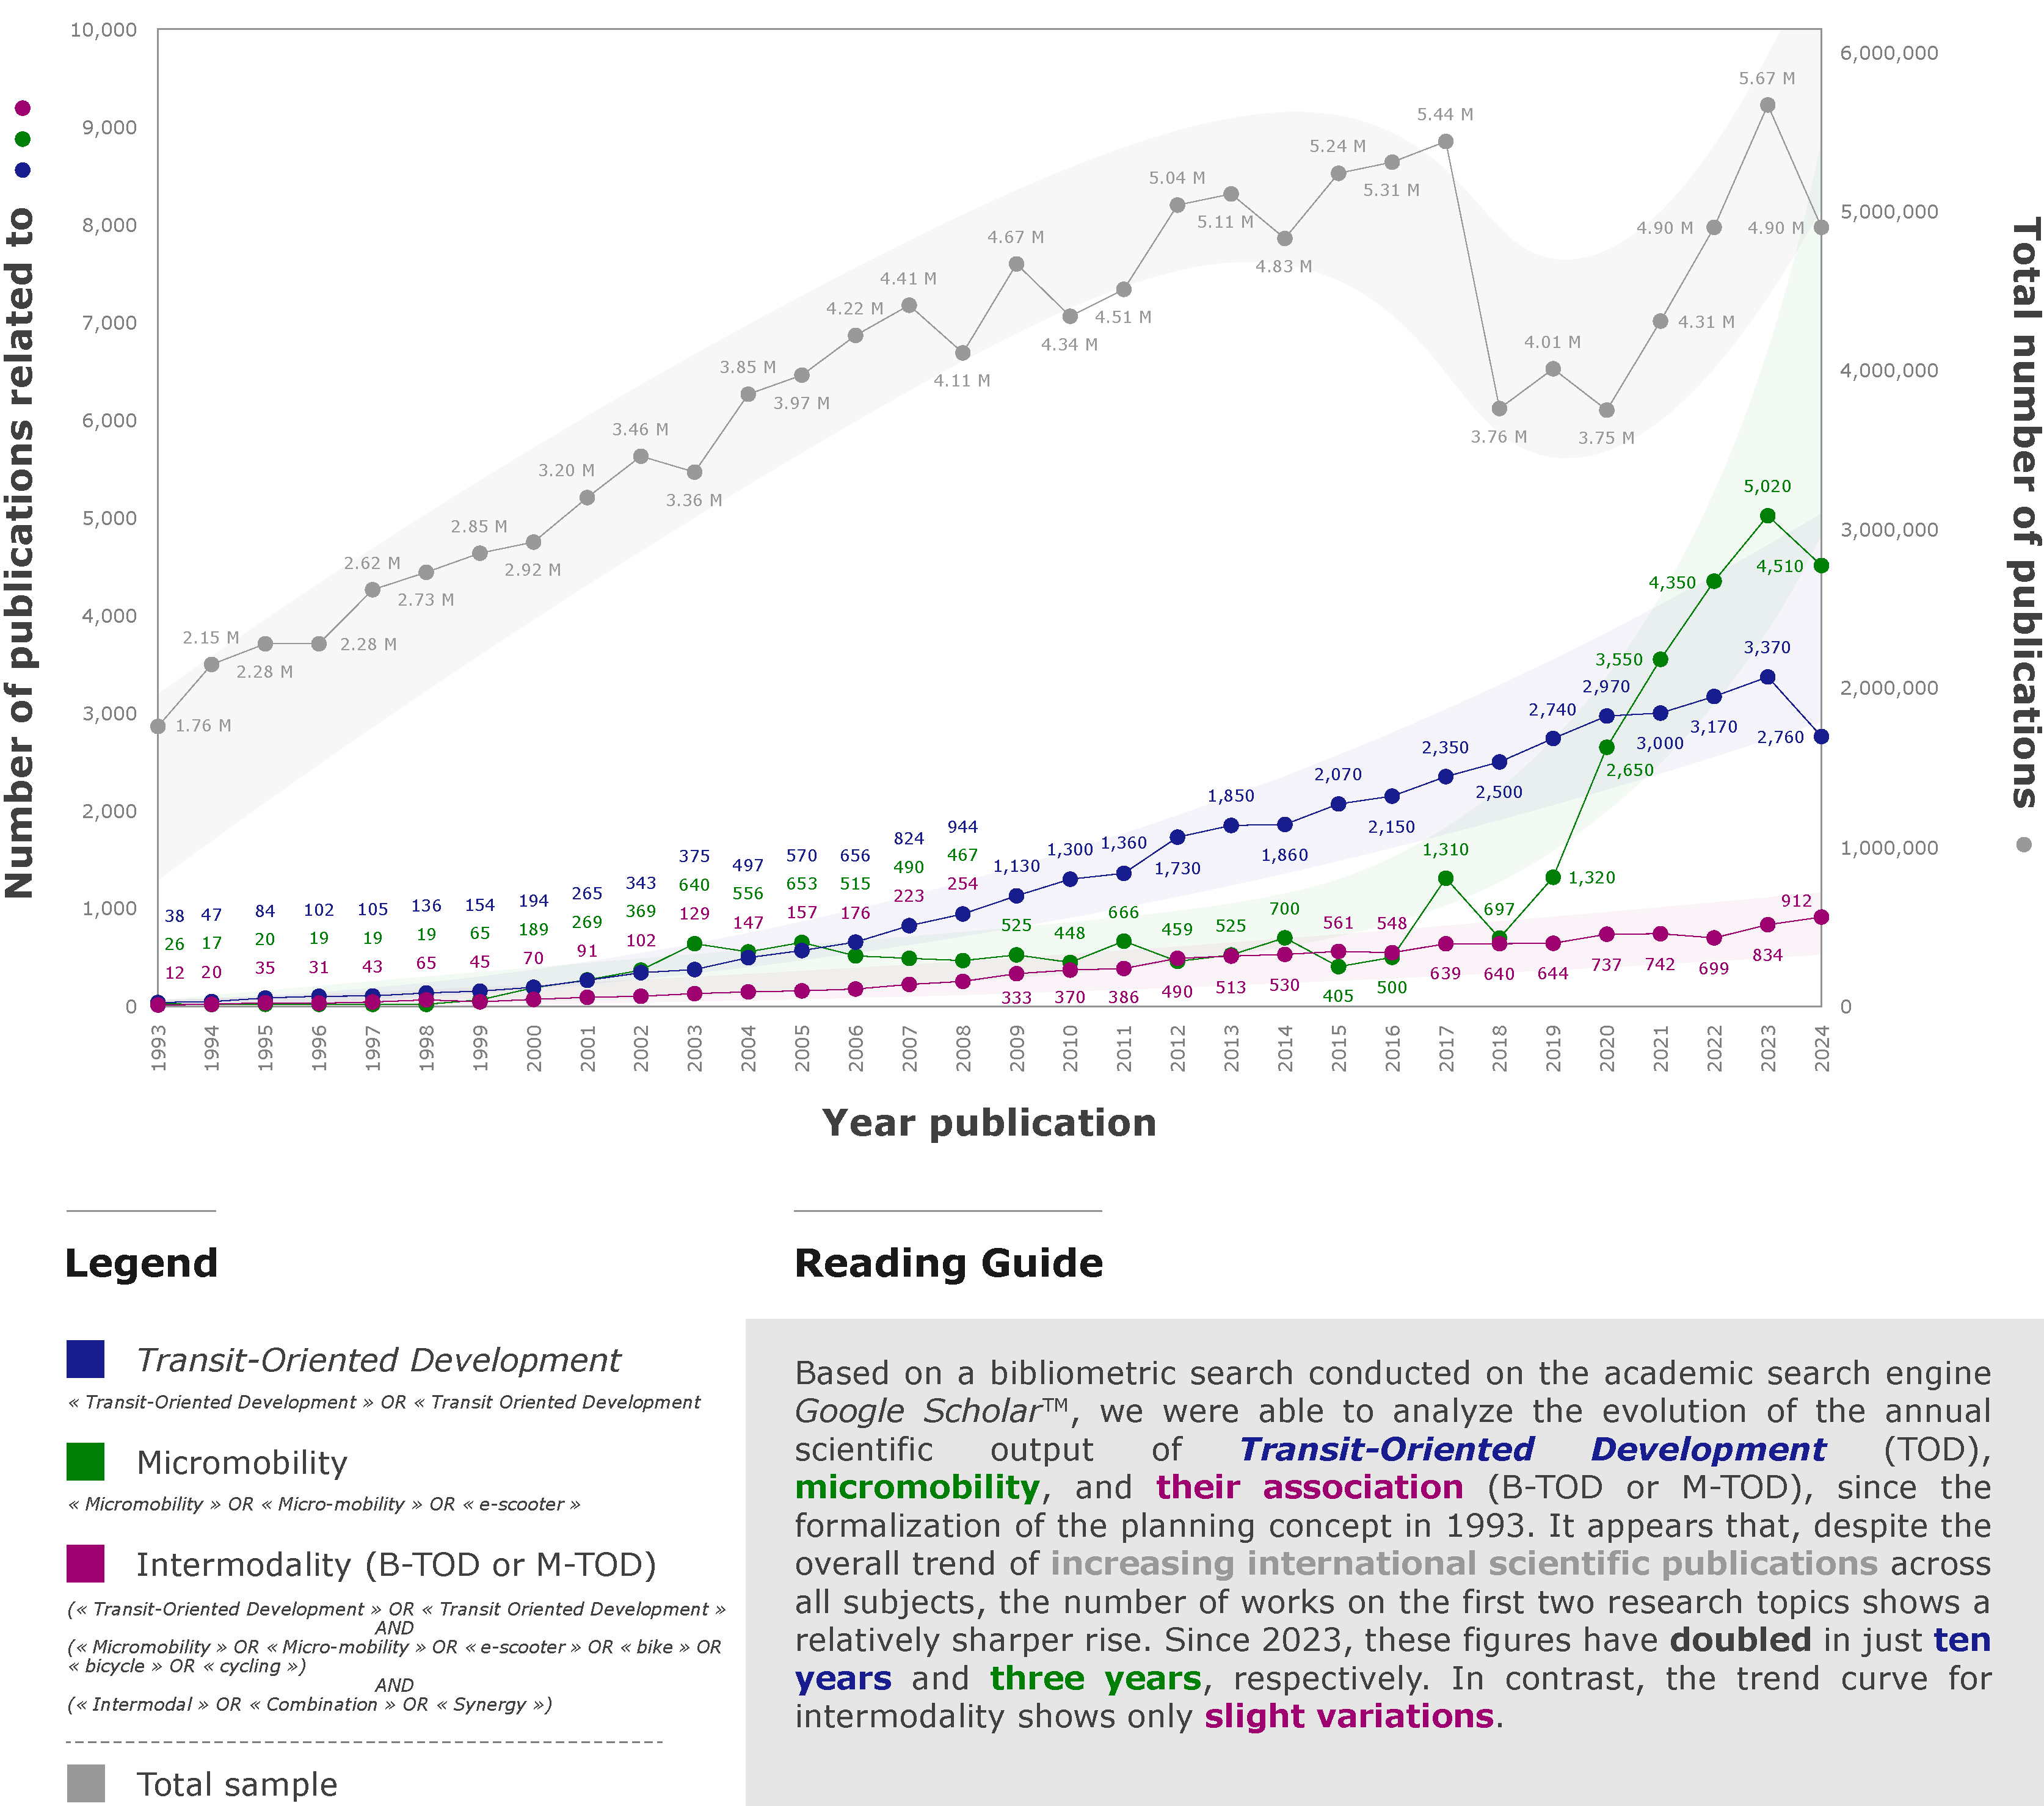
\includegraphics[width=1\columnwidth]{src/Figures/Chap-1/EN_Chronologie_publications_TOD_MIL.pdf}}
    \vspace{5pt}
    \begin{flushright}\scriptsize{
    Source: bibliometric data from \Marque{Google Scholar} exported on February 2, 2025
    \\
    Author: \textcolor{blue}{Dylan Moinse (2025)}
    }\end{flushright}
\end{figure}

% M-TOD + Transition
One of the recent developments in \acrshort{TOD} explored in this chapter concerns the integration of light individual mobility. These modes of transportation complement traditional infrastructures by providing effective solutions to the challenges of the \Commas{first and last miles}. However, knowledge of this form of intermodality, particularly in its interaction with urban forms, remains limited. This is especially true for emerging mobilities that make up this family of modes, whose interactions with \acrshort{TOD} remain largely unexplored. A simple lexical search on the themes of \acrshort{TOD} and micromobility illustrates how these topics are gaining increasing interest in academic research, as shown in \hyperref[fig-chap1:trends-google-scholar]{Figure~\ref{fig-chap1:trends-google-scholar}} (page~\pageref{fig-chap1:trends-google-scholar}). Nevertheless, this growing interest has not yet translated into a true synergy between these two fields of study, which remain underrepresented together in the scientific literature. This chapter, which sets the theoretical framework for our research, thus concludes with the observation of a knowledge gap \textsl{a priori} on a topic recently rediscovered in the context of \acrshort{TOD}. This gap is also highlighted by \textcolor{blue}{Wei} \textcolor{blue}{\textcite[90]{kang_university_2020}}\index{Kang, Wei|pagebf}\index{Aguiléra, Anne|pagebf}\index{Rallet, Alain|pagebf}, who points out in his doctoral thesis the low number of studies dedicated to intermodality between new mobility services, such as the \acrshort{DBS}, and public transport. Similarly, \acrshort{PeS} and \acrshort{DESS} have been marginally studied, beyond issues related to trauma or accidentology, even though their intermodal potential is widely reported \textcolor{blue}{\autocite{richer_dossier_2021}}\index{Richer, Cyprien|pagebf}. Conducting rigorous empirical studies on these forms of intermodality appears to be a requirement to measure and understand behaviors related to \textsl{bike-and-ride} and \textsl{scoot-and-ride} \textcolor{blue}{\autocite[13]{bortoli_consequential_2020}}\index{Bortoli, Anne de|pagebf}\index{Christoforou, Zoi|pagebf}. Given this assessment, we have chosen to initiate an exploratory study on what we call \acrshort{M-TOD}, by compiling existing works on this topic, which will be presented in the next chapter.%%Translated%%

% ___________________________________________
     \newpage
     
% Valorisation scientifique
    \begin{tcolorbox}[colback=white!5!white,
                      colframe=blue!75!blue,
                      title=Valorization
                      \\
                      Chapitre~1]
\Large{\textcolor{blue}{\textbf{Seminars:}}}
    \\\\
\small{\textcolor{blue}{\textcite{moinse_transit-oriented_2021}}. Le Transit-Oriented Development, un urbanisme axé sur les transports en commun, intégrant les micro-mobilités émergentes. Une investigation sur les trottinettes personnelles en intermodalité, dans la région Hauts-de-France. \textsl{Rencontres TerriTrans - MoTAU}, Paris.
\\
\footnotesize{\url{https://hal.science/hal-03473391}} (\textbf{C-COM})}
    \\\\
\small{\textcolor{blue}{\textcite{moinse_modeurbain_2021}}. Le modèle urbain du Transit-Oriented Development revisité par les mobilités émergentes? Une investigation sur le territoire de la région Hauts-de-France. \textsl{Rencontres Internationales en Urbanisme de l'APERAU}, Rabat.
\\
\footnotesize{\url{https://shs.hal.science/halshs-03507291}} (\textbf{C-COM})}
    \\\\
\small{\textcolor{blue}{\textcite{moinse_modeurbain_2020}}. Le modèle urbain du Transit-Oriented Development revisité par les micro-mobilités émergentes? Une investigation sur le territoire de la région Hauts-de-France. \textsl{(Post-)Doctoriales AME 2020}, Le Croisic.
\\
\footnotesize{\url{https://shs.hal.science/halshs-03507482}} (\textbf{C-COM})}
    \\\\
\small{\textcolor{blue}{\textcite{moinse_etat_2020}}. État de l'art sur l'usage des trottinettes électriques en libre-service sans station. \textsl{Journées Transports \& Déplacements du Réseau Scientifique et Technique} (JTD RST). 
\\
\footnotesize{\url{https://shs.hal.science/halshs-03507375}} (\textbf{C-COM})}
    \\\\
\Large{\textcolor{blue}{\textbf{Communication:}}}
    \\\\
\normalsize{\textcolor{blue}{\textcite{moinse_exploring_2023}}. \foreignlanguage{english}{\textsl{Exploring Val d'Europe's Urban Development in Marne-la-Vallée: A Guided Walking Tour of the TOD Project}}, Présentation de terrain, Paris
\\
\footnotesize{\url{https://shs.hal.science/halshs-04212064}}}
    \end{tcolorbox}

    % ___________________________________________
    % Subbibliography
    \newpage
    \sectionheader{Bibliography of Chapter~1}
    \begingroup
    \renewcommand{\bibfont}{\scriptsize}
\printbibliography[segment=\therefsegment, heading=subbibintoc, title={Bibliography of Chapter~1}, label=chap1:bibliographie]
    \endgroup
    \end{refsegment}

%% ______________________________ %%
% CHAPTER 2
%------------------------------%
%% ✎ Dylan (V1) %%%%%%%%% ✅ %%
%% ✎ Alain (V2) %%%%%%%%% ✅ %%
%% ✎ Dylan (V3) %%%%%%%%% ✅ %%
%------------------------------%

%%%%%%%%%%%%%%%%%%%%%%%%%%%%%%%%
% Chapter 2
\chapterheader{Systematic Literature Review}
\chapter
{Systematic Literature Review on Transit-Oriented Development and the Integration of Light Individual Mobility
    \label{chap2:titre}
    }
    \begin{refsegment}

    % Chapter 2 Background
    \AddToShipoutPictureBG*{%
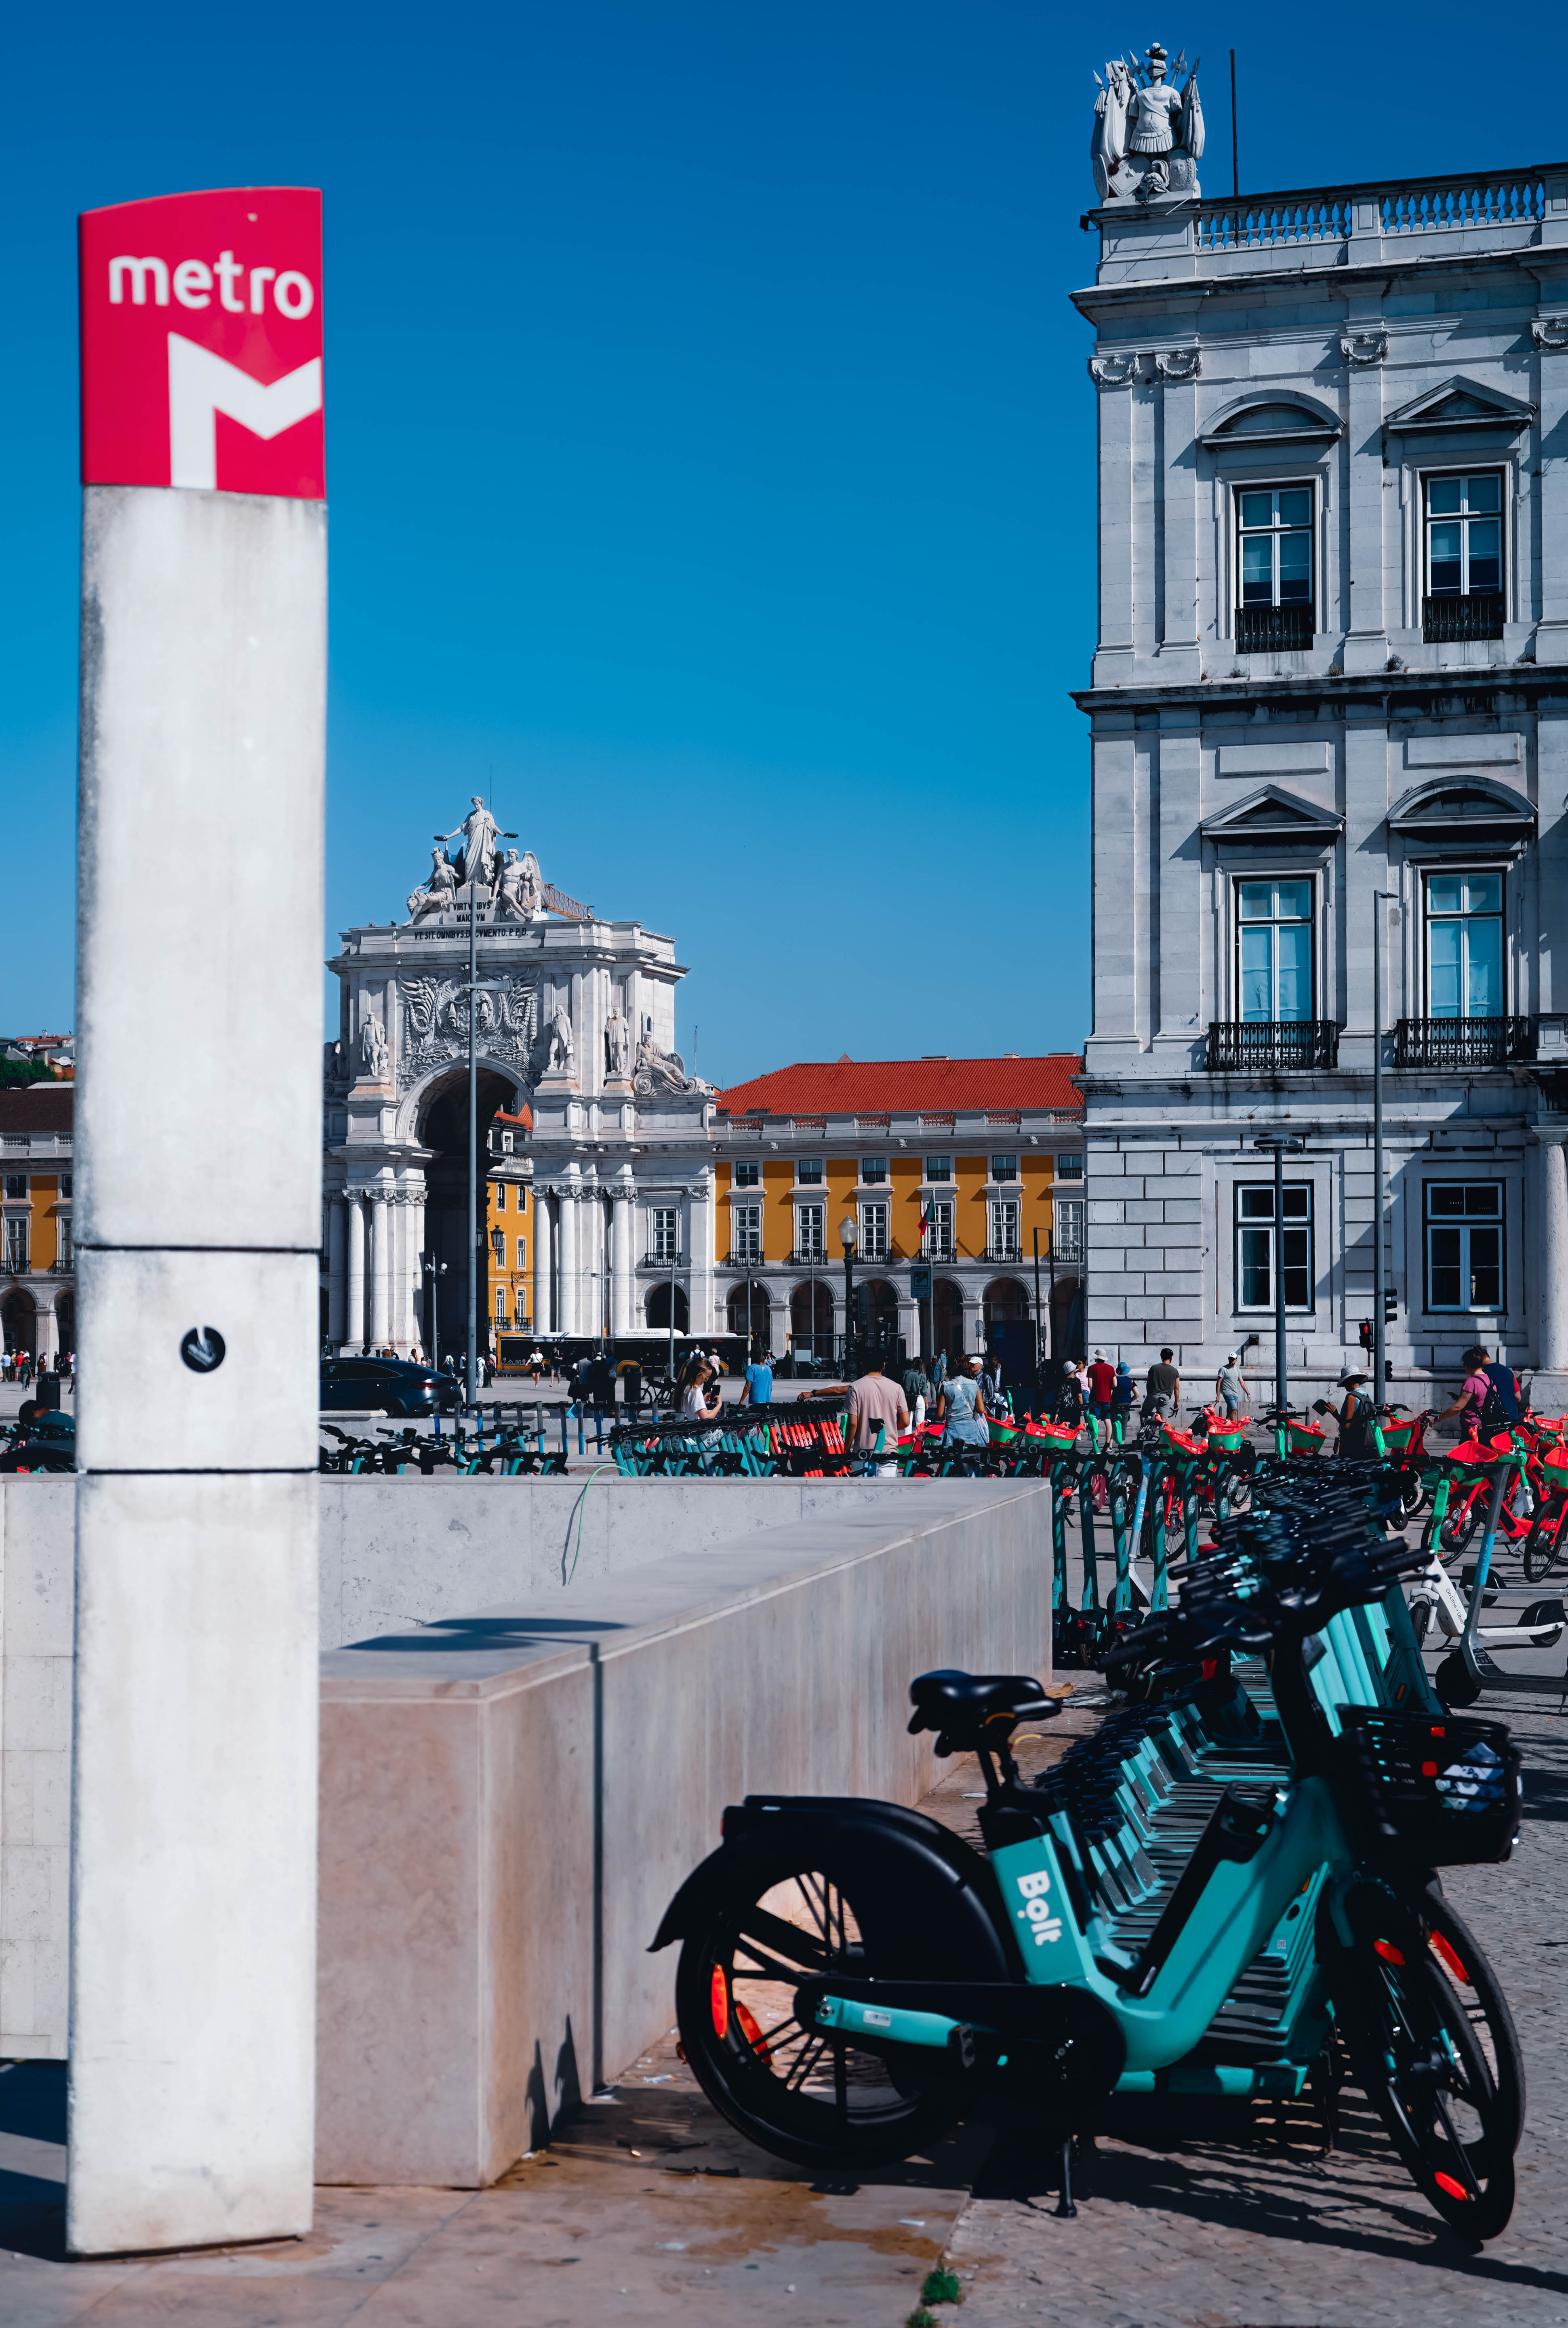
\includegraphics[width=\paperwidth,height=\paperheight]{src/Figures/Arriere_plan/Arriere_plan_Chap_2.jpg}
    }

% Rectangle
\AddToShipoutPictureBG*{
  \begin{tikzpicture}[remember picture,overlay]
    \node[fill=white, opacity=0.75, text width=\paperwidth, minimum height=12.25cm, anchor=north] 
    at ([yshift=-2cm]current page.north) {};
  \end{tikzpicture}
}

% Source
\AddToShipoutPictureFG*{
  \AtPageLowerRight{
    \raisebox{1cm}{
      \hspace{16cm}
      
\begin{tikzpicture}
        \node[fill=white, rounded corners=5pt, inner sep=5pt, align=center] {
          \tiny{Photography: \textcolor{blue}{Dylan Moinse (2023)}}
        };
      \end{tikzpicture}
    }
  }
}

    % ___________________________________________
    % Mini Table of Contents
    \cleardoublepage
    \setcounter{tocdepth}{2}
    % Redefine local table of contents title
    \renewcommand{\localcontentsname}{Table of Contents of Chapter~2}
\localtableofcontents

% Reset section numbering
\setcounter{section}{0}

%%%%%%%%%%%%%%%%%%%%%%%%%%%%%%%%
% Chapter 2
\newpage
\section*{Key Points of Chapter~2
    \label{chap2:graphical-abstract}
    }
    \markright{Chapter Preamble}{}

\begin{figure}[h!]\vspace*{4pt}
        \caption*{}
        \label{graphical-abstract-chap2}
        \centerline{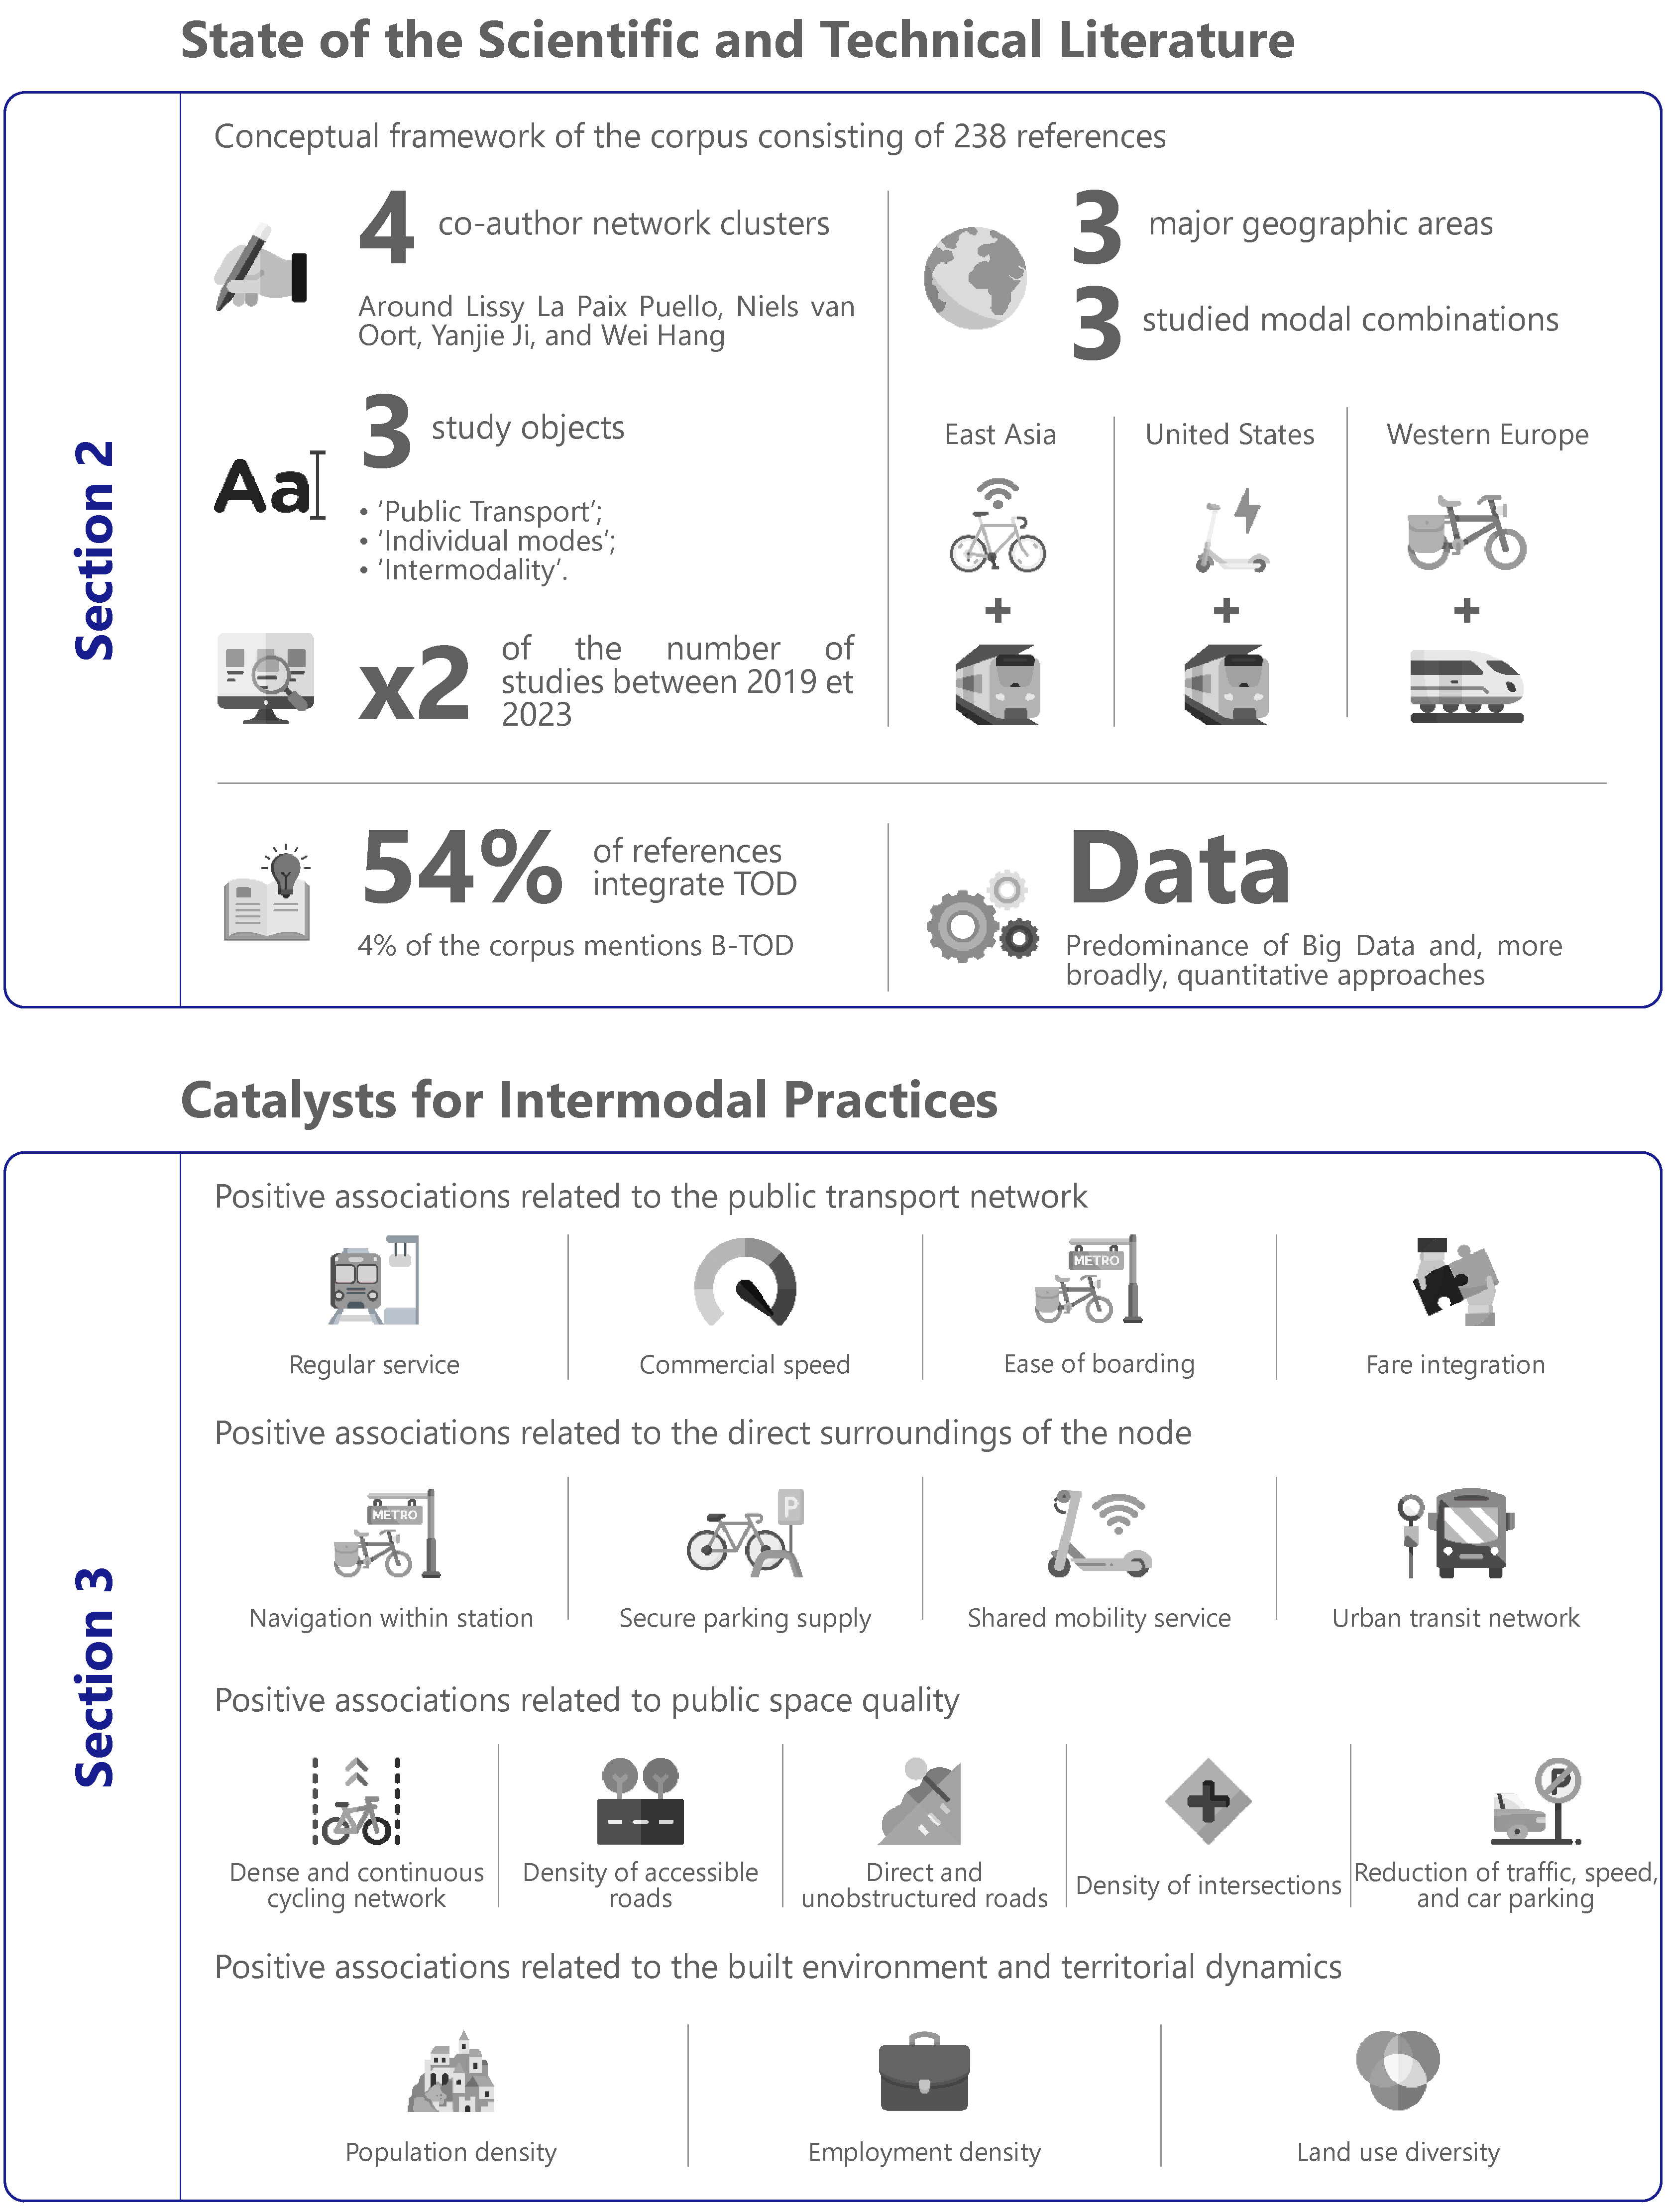
\includegraphics[width=1\columnwidth]{src/Figures/Graphical-abstract/EN_Graphical_abstract_chap2.pdf}}
        \vspace{5pt}
    \end{figure}

    % ___________________________________________
    % Preambule
    \newpage
    \begin{tcolorbox}[colback=white!5!white,
                      colframe=blue!75!blue,
                      title=
                      \bigskip
                      \center{\textbf{Preambule of Chapter~2}}
                      \\
                      \raggedright{\small{Chapter composed of \pagedifference{chap2:titre}{chap3:titre} pages, including \pagedifference{chap2:bibliographie}{chap3:titre} pages of bibliography}}
                      \bigskip]
\Large{\textbf{\textcolor{blue}{Abstract:}}}
    \\
    \small{
This chapter provides an overview of the current research on Transit-Oriented Development (TOD) promoting and supported by light individual mobility. This bibliometric study and bibliographical analysis are presented as a systematic literature review (SLR) compiling 238 scientific publications. The goal is to provide a state of knowledge on the B-TOD and M-TOD, with a preference for using the SLR due to its capacity to conduct an exhaustive analysis of the scientific literature on this research topic.%%Translated%%
    \\
The creation of this corpus involved selecting scientific articles, conference papers, book chapters, theses, and research reports in both English and French. These academic works were examined according to predefined criteria in order to identify all research addressing the intersection between light individual mobility and public transport (see \hyperref[chap2:protocole-methodologique-rsl]{Section~1}, page~\pageref{chap2:protocole-methodologique-rsl}).%%Translated%%
    \\
Initially, this bibliographic study examined the temporal, geographic, and institutional contexts influencing research on M-TOD, as well as the conceptual and methodological frameworks defined to assess this urban model (see \hyperref[chap2:analyse-documentation-rsl]{Section~2}, page~\pageref{chap2:analyse-documentation-rsl}). The analysis of the chronological and spatial distribution of the references revealed a growing interest in traveler intermodality, centered around three countries at a local scale, with modal combinations evolving over time. The adopted methodology tends towards developing geostatistical analyses and models, facilitated by the development of computing tools and Big Data.%%Translated%%
    \\
The third part of this chapter focuses on analyzing the lessons drawn from the studies reviewed, with particular attention to the various components of B-TOD and M-TOD, conceptualized under the term of the \Commas{7Ds} (see \hyperref[chap2:caracterisation-btod-environnement-urbain-choix-individuels]{Section~3}, page~\pageref{chap2:caracterisation-btod-environnement-urbain-choix-individuels}). The characterization of M-TOD revealed both similarities and divergences, highlighting a positive association with population and employment density, land use diversity, treatment of public spaces, and the quality of public transport services. Various impacts on mobility behaviors, mainly commuter-based, and on the environment were identified, such as a decrease in carbon footprint, improved accessibility to destinations for a larger portion of the population, as well as the existence of social inequalities in terms of accessibility.%%Translated%%
    \\
Finally, the SLR paves the way for a critical reading of the gaps in the scientific literature and the challenges of M-TOD (see \hyperref[chap2:conclusion]{chapter conclusion}, page~\pageref{chap2:conclusion}).%%Translated%%
    }
    \tcblower
\Large{\textbf{\textcolor{blue}{Keywords:}}}
    \\
    \small{
Bibliometric analysis;
Network analysis;
Socio-economic characteristics;
Urban characteristics;
Scientific mapping;
Mobility behaviors;
Impacts;
Critical reading of M-TOD;
International perspective;
Systematic literature review
    }
    \end{tcolorbox}

% ___________________________________________
% 2.*.
\newpage
\needspace{1\baselineskip} % Reserve space
\addcontentsline{toc}{section}{Introduction of Chapter~2}
\sectionheader{Introduction of Chapter~2}
\section*{Introduction of Chapter~2
    \label{chap2:introduction}
    }
    \markright{Introduction of Chapter~2}{}

    % Citation
    \begin{displayquote}
\Commas{\textsl{Next to innovations within transport modes, the strengths and weaknesses identified above also define the scope for transport mode combinations between transport modes. One such combination is between transport modes that give a relatively higher spatial access because of their speed with slower modes that have some other advantage.} [\dots] \foreignlanguage{english}{\textsl{Combinations between fast transit (such as trains) and non-motorized modes, particularly the bike, allow overall high door-to-door speed between virtually ubiquitous origin destinations. The train-bike combination is a particularly strong one: the train is much faster than other public transport, and the bike combines ubiquitous access with relatively high speeds (higher than walking but often also competitive with conventional buses or trams, and in certain environments even cars). In countries where both biking infrastructure and railway services are extensive~–~such as the Netherlands~–~this combination is so developed that it can be considered a transport mode in itself, and in many contexts directly competitive with the car.}} [\dots] \textsl{But also, the train-bike combination might integrate into a hybrid system which is both fast and flexible, and thus fully competitive with the car.} [\dots] \textsl{This type of multi-modal behaviour is now limited, but could become generalized in the future.} [\dots] \textsl{What if such a hybrid, highly adaptive behaviour and transportation system became dominant?}}

\textcolor{blue}{Luca} \textcolor{blue}{\textcite[80-81, 220]{bertolini_planning_2017}}\index{Bertolini, Luca|pagebf}. \foreignlanguage{english}{\textsl{Planning the Mobile Metropolis: Transport for People, Places and the Planet}}, Ed. Red Globe Press, Londres, 253~p. ISBN: \href{https://search.worldcat.org/fr/title/1004435849}{978-0-230-30877-0}
    \end{displayquote}

    % Introduction
\lettrine[lines=3, findent=8pt, nindent=0pt]{\lettrinefont T}{his} chapter aims to present the current state of knowledge addressing the redefinition of \acrfull{TOD} in connection with the renewed interest in light individual mobility, with the goal of defining the concept of \acrfull{B-TOD} expanded by light individual mobility. To collect, analyze, and contextualize research on this topic, a \acrfull{SLR} was conducted. Thus, only academic publications in English or French that focus on studying this form of \gls{intermodality}, from a geographical and urban perspective, were included in this bibliographic analysis.%%Translated%%

    % Justification B-TOD / M-TOD
In light of the potential of light individual mobility to expand the \gls{intermodal accessibility} of public transport nodes \textcolor{blue}{\autocite[118]{cottrell_transforming_2007}}\index{Cottrell, Wayne~D.|pagebf}, the underlying goal of this critical analysis of the scientific literature regarding the emerging concept of \acrfull{M-TOD} is to gather and better understand how this modal combination can promote urban design conducive to the development of alternative modes of transportation. Starting from the observation that the combination of public transport with light individual mobility, just like combined walking, represents the most effective form of integration \textcolor{blue}{\autocite[50]{sebban_complementarite_2003, yang_study_2013}}\index{Sebban, Annie-Claude|pagebf}\index{Yang, Rongrong|pagebf}\index{Yan, Hai|pagebf}\index{Xiong, Wen|pagebf}\index{Liu, Tao|pagebf}, both economically, socially, and environmentally—three dimensions valued by \acrshort{TOD} \textcolor{blue}{\autocite[85]{cervero_bike-and-ride_2013}}\index{Cervero, Robert|pagebf}\index{Caldwell, Benjamin|pagebf}\index{Cuellar, Jesus|pagebf}—the research question addressed by this \acrshort{SLR} is twofold. It seeks to justify the integration of light individual mobility into public transport systems as opposed to other forms of intermodality such as park-and-ride, while identifying the challenges inherent in the urban model of \acrshort{M-TOD}.%%Translated%%

    % Justification RSL
The value of conducting a \acrshort{SLR} lies in its ability to gather, assess, and synthesize existing knowledge on a complex research topic that blends two interdisciplinary objects of study, not only involving urban planning and mobility but also a multitude of disciplines related to urban systems, infrastructure, and populations. The innovative approach of the \acrshort{SLR} distinguishes itself from traditional literature reviews by its pursuit of enhanced objectivity, its goal of comprehensiveness, the formulation of specific questions, and the increased transparency of the steps involved in the process. While this method is primarily used in the exact sciences, the \acrshort{SLR} is proving its effectiveness in the \acrfull{HSS} through gradual adjustments. Therefore, developing such a method for an original and recent research topic offers several advantages. It allows for the identification and evaluation of existing studies, adopting a global and clear vision of the state of scientific knowledge, spotting emerging trends and the evolution of research, as well as identifying underexplored aspects. Consequently, the \acrshort{SLR} also helps to guide future research, as is the case with this doctoral research.%%Translated%%

    % Outline Announcement 1
We will first present in detail the methodological protocol for composing the academic corpus (\hyperref[chap2:protocole-methodologique-rsl]{Section~1}, page~\pageref{chap2:protocole-methodologique-rsl}), which will include the formulation of the research questions (\hyperref[chap2:formulation-questions-recherche]{Subsection~1.1}, page~\pageref{chap2:formulation-questions-recherche}), the documentary search strategy (\hyperref[chap2:strategie-recherche-documentaire]{Subsection~1.2}, page~\pageref{chap2:strategie-recherche-documentaire}), the processes of selecting scientific publications (\hyperref[chap2:selection-publications-scientifiques]{Subsection~1.3}, page~\pageref{chap2:selection-publications-scientifiques}) and extracting the collected data, as well as the examined aspects (\hyperref[chap2:extraction-donnees-aspects-consideres]{Subsection~1.4}, page~\pageref{chap2:extraction-donnees-aspects-consideres}).%%Translated%%

    % Outline Announcement 2
Once the methodology is presented, we will highlight the characteristics of the scientific literature and research practices on this topic (\hyperref[chap2:analyse-documentation-rsl]{Section~2}, page~\pageref{chap2:analyse-documentation-rsl}), through the analysis of metadata from the documentation (\hyperref[chap2:etat-litterature-scientifique-internationale-btod]{Subsection~2.1}, page~\pageref{chap2:etat-litterature-scientifique-internationale-btod}) and the conceptual and methodological frameworks of the bibliographic references (\hyperref[chap2:cadres-conceptuels-methodologiques]{Subsection~2.2}, page~\pageref{chap2:cadres-conceptuels-methodologiques}).%%Translated%%

    % Outline Announcement 3
The third part of this \acrshort{SLR} will be dedicated to a synthetic presentation of the \Commas{\acrfull{7Ds}} and the main lessons serving as guiding principles for the TOD (\hyperref[chap2:caracterisation-btod-environnement-urbain-choix-individuels]{Section~3}, page~\pageref{chap2:caracterisation-btod-environnement-urbain-choix-individuels}), by examining the association between the integration of light individual mobility and the influence of population density (\hyperref[chap2:densite-population]{Subsection~3.1}, page~\pageref{chap2:densite-population}), functional diversity (\hyperref[chap2:diversite-fonctionnelle]{Subsection~3.2}, page~\pageref{chap2:diversite-fonctionnelle}), the treatment of public spaces (\hyperref[chap2:traitement-espaces-publics]{Subsection~3.3}, page~\pageref{chap2:traitement-espaces-publics}), intermodal accessibility (\hyperref[chap2:accessibilite-intermodale]{Subsection~3.4}, page~\pageref{chap2:accessibilite-intermodale}), distances to and from transport nodes (\hyperref[chap2:distances-premiers-derniers-km]{Subsection~3.5}, page~\pageref{chap2:distances-premiers-derniers-km}), mobility demand management (\hyperref[chap2:gestion-demande-mobilite]{Subsection~3.6}, page~\pageref{chap2:gestion-demande-mobilite}), socio-demographic characteristics of users (\hyperref[chap2:sociodemographie-usagers]{Subsection~3.7}, page~\pageref{chap2:sociodemographie-usagers}), mobility behaviors (\hyperref[chap2:comportements-mobilite]{Subsection~3.8}, page~\pageref{chap2:comportements-mobilite}) and the impacts of these intermodal practices on mobility systems and urban systems (\hyperref[chap2:impacts-systemes-urbain-mobilite]{Subsection~3.9}, page~\pageref{chap2:impacts-systemes-urbain-mobilite}).%%Translated%%

    % Outline Announcement 4
In conclusion, we will suggest future research directions concerning the integration of light individual mobility into \acrshort{TOD}, which will contribute to this doctoral thesis (\hyperref[chap2:conclusion]{conclusion of Chapter~2}, page~\pageref{chap2:conclusion}).%%Translated%%

    % 2.1.
    \newpage
    \needspace{1\baselineskip} % Reserve space
    \sectionheader{Methodology of the Systematic Literature Review}
\section{Methodological Protocol of the Systematic Literature Review
    \label{chap2:protocole-methodologique-rsl}
    }
    
    % State of the Art SLR
The methodological procedure underlying the development of a \acrshort{SLR} is constantly evolving due to its relatively recent emergence in the fields of \acrshort{HSS} and ongoing discussions about the methodological limitations associated with it. The \acrshort{SLR} conducted in this chapter follows the techniques outlined in the reference article dedicated to the execution of a thematic and qualitative \acrshort{SLR} in a medical scientific journal, written by \textcolor{blue}{\textcite[3-7]{thomas_methods_2008}}\index{Thomas, James|pagebf}\index{Harden, Angela|pagebf}. Considering the nuances in performing an \acrshort{SLR} across disciplines \textcolor{blue}{\autocite[738]{padeiro_transit-oriented_2019}}\index{Padeiro, Miguel|pagebf}\index{Louro, Ana|pagebf}\index{Costa, Nuno Marques de|pagebf}, the developed methodological protocol is based on lessons drawn from various \acrshort{SLR}\textcolor{blue}{s} examining \acrshort{TOD} and light individual mobility. The method used draws on techniques and reflections from various \acrshort{SLR}\textcolor{blue}{s}, one focusing on the links between \acrshort{TOD} and gentrification \textcolor{blue}{\autocite[738]{padeiro_transit-oriented_2019}}\index{Padeiro, Miguel|pagebf}\index{Louro, Ana|pagebf}\index{Costa, Nuno Marques de|pagebf}, and another on the integration of light individual mobility with public transportation systems \textcolor{blue}{\autocite[4]{oeschger_micromobility_2020}}\index{Oeschger, Giulia|pagebf}\index{Carroll, Páraic|pagebf}\index{Caulfield, Brian|pagebf}. Several existing literature reviews also guided the design of our \acrshort{SLR}, particularly those examining bicycles and electric micromobility \textcolor{blue}{\autocite[3]{sengul_impacts_2021}}\index{Sengül, Buket|pagebf}\index{Mostofi, Hamid|pagebf}, electric scooter services \textcolor{blue}{\autocite[4]{bozzi_shared_2021}}\index{Bozzi, Alberica Domitilla|pagebf}\index{Aguiléra, Anne|pagebf}, the choice of cycling routes \textcolor{blue}{\autocite[2]{pritchard_revealed_2018}}\index{Pritchard, John~P.|pagebf}, and the use of \textsl{Big Data} in mobility \textcolor{blue}{\autocite[36]{neilson_systematic_2019}}\index{Neilson, Alex|pagebf}\index{Indratmo|pagebf}\index{Daniel, Ben|pagebf}\index{Tjandra, Stevanus|pagebf}.%%Translated%%

    % Selection
Moreover, this bibliographic research is inspired by the methodological guide intended to produce a literature review in the fields of urban planning and mobility, as adapted by the US national academic organization \textcolor{blue}{\textcite{transportation_research_board_of_the_national_academies_literature_2015}}\index{Transportation Research Board@\textsl{Transportation Research Board}|pagebf}. This report notably identifies six main steps to constitute an \acrshort{SLR}: defining the research subject (i), selecting appropriate libraries and bibliographic databases for the defined subject (ii), formulating an expression using keywords (iii), defining relationships between terms to develop an advanced search (iv), checking the collection of texts gathered (v), and organizing the data for analysis (vi) \textcolor{blue}{\autocite[2-18]{transportation_research_board_of_the_national_academies_literature_2015}}\index{Transportation Research Board@\textsl{Transportation Research Board}|pagebf}. Furthermore, the process of selecting scientific publications for this \acrshort{SLR} embraces the three stages established by \textcolor{blue}{\textcite[2544]{jain_systematic_2020}}\index{Jain, Deepshikha|pagebf}\index{Singh, Ekta|pagebf}\index{Ashtt, Rashmi|pagebf}:
    \begin{customitemize}
        \item The initial exclusion phase involves analyzing the metadata from bibliographic references, including the title, abstract, and associated keywords, to assess their relevance to the research topic;
        \item The intermediate exclusion phase involves critical reading of the introduction and conclusion of each retained document to further filter publications that align with the research objectives set in the \acrshort{SLR};
        \item The final exclusion phase engages a full reading of the studies included in the \acrshort{SLR} to ensure the quality of the selection process.
    \end{customitemize}
Following these three sequences, the inclusion process ensures a methodical approach to identifying relevant academic sources related to the specified research topic.%%Translated%%

    % Advantages of SLR
Compared to a conventional literature review, the \acrshort{SLR} acquires the status of being \Commas{systematic} when it is structured around a formulated research question, the identification of relevant works in line with the defined topic, and a clear explanation of the methodology followed. In this sense, the \acrshort{SLR} holds several comparative advantages \textcolor{blue}{\autocite[2]{transportation_research_board_of_the_national_academies_literature_2015}}\index{Transportation Research Board@\textsl{Transportation Research Board}|pagebf}:
    \begin{customitemize}
        \item The problem-solving capacity enabled by the comprehensive coverage of existing knowledge on a specific topic;
        \item The confrontation of previous and competing studies, facilitating the understanding of the existing academic discourse;
        \item The validation of the research methods applied by questioning the reliability of the chosen approaches;
        \item The confirmation of the necessity to continue research by highlighting emerging study areas;
        \item The guidance of research efforts by providing perspectives that shed light on the current state of knowledge and suggest promising directions for future research initiatives.
    \end{customitemize}
With these advantages, the \acrshort{SLR} establishes a solid foundation to probe the scientific literature, contributing to greater methodological rigor, a fine analysis of existing research, and a roadmap to guide subsequent studies.%%Translated%%

    % 2.1.1.
    \needspace{1\baselineskip} % Reserve space
\subsection{Formulation of Research Questions
    \label{chap2:formulation-questions-recherche}
    }
    
    % Questions and objectives
The primary goal of this \acrshort{SLR} is to provide a deep understanding of the existing knowledge and practices related to urban planning oriented towards public transportation, supported by light individual mobility, while identifying the factors that facilitate or hinder the implementation of this urban model and assessing its effects on mobility and territories. In this regard, the \acrshort{SLR} aims to first examine and discuss the role of the bicycle within the planning model. Although the integration of this mode of transport was considered from the conceptualization of \acrshort{TOD}, its potential seems to remain underexplored. It is with this perspective that this literature review seeks to characterize its iteration, known as \acrshort{M-TOD}. Additionally, we aim to update it by incorporating the exploration of emerging \gls{micromobility} options. These, due to their innovative nature, are likely to interact with and transform the foundations of \acrshort{M-TOD} in turn.%%Translated%%

    % Research Questions
The following reading grid, centered around six research questions, guides the \acrshort{SLR}:
    \begin{customitemize}
        \item What urban factors and public policies promote the integration of bicycles and micromobility options into public transport systems? Conversely, does this form of mobility influence territorial configurations?
        \item What are the effects of this modal combination in terms of economic development, social cohesion, and environmental sustainability?
        \item Is there a relevant perimeter to define a transit-oriented development area based on light individual mobility? Does the size of these influence areas vary according to certain parameters?
        \item What urban planning practices and governance models prove to be innovative and effective in promoting such urban development?
        \item Can the \acrshort{M-TOD} be considered an internationally recognized and replicable urban model?
        \item What are the main challenges to be addressed when reflecting on and applying an \acrshort{M-TOD} strategy?
    \end{customitemize}%%Translated%%

    % 2.1.2.
    \needspace{1\baselineskip} % Reserve space
\subsection{Search Strategy for the Literature Review
    \label{chap2:strategie-recherche-documentaire}
    }

    % Online Research
The initial data collection phase is carried out using online searches, utilizing bibliographic databases offering transdisciplinary coverage. This documentation collection step ensures the capture and listing of a comprehensive corpus of bibliographic references from scientific literature and grey literature
    \footnote{~
        In this context, scientific literature refers to peer-reviewed academic publications, including articles published in scientific journals, conference proceedings, book chapters, and research theses. Grey literature, as defined by \acrfull{AFNOR} and the Luxembourg Convention on Grey Literature, includes \Commas{\textsl{typed or printed documents, often provisional in nature, reproduced and distributed in fewer than a thousand copies, outside the commercial publishing and distribution channels}}~\textcolor{blue}{\autocite[30]{schopfel_comprendre_2015}}\index{Schöpfel, Joachim|pagebf}. Grey literature encompasses \Commas{\textsl{what is produced by all levels of government, universities, businesses, and industry, in printed or electronic form, but not controlled by commercial publishing}}~\textcolor{blue}{\autocite{national_grey_literature_collection_luxembourg_nodate}}\index{National Grey Literature Collection|pagebf}. Recently, \textcolor{blue}{Joachim} \textcolor{blue}{\textcite[9]{schopfel_vers_2012}}\index{Schöpfel, Joachim|pagebf} proposed a renewed definition of this type of literature, considering it as \Commas{\textsl{a document produced by government, administration, education and research, business and industry, in printed or electronic form, protected by intellectual property rights, of sufficient quality to be collected and preserved by a library or institutional archive, and not controlled by commercial publishing}}.
}. In this \acrshort{SLR}, online searches include scientific articles, conference proceedings, book chapters, master's or doctoral research theses, and public research reports. However, they exclude, among others, scientific preprints, technical or policy documents, private study reports, public statements, or newsletters. It is worth noting that the bibliographic inventory related to \acrshort{M-TOD} was initially created between December 3 and 8, 2021. Later, due to the emerging nature of this topic, an update to the data collection was carried out between April 10 and 13, 2023, to include the most recent publications.%%Translated%%

    % Online Research Step
The data collection for this \acrshort{SLR} was carried out through an \acrfull{EN~Search}, or \(S_{EN}\), and an \acrfull{FR~Search}, or \(S_{FR}\), using various online platforms that have solid recognition in the academic sphere. The academic resources cited below were selected due to their extensive coverage, accessibility, and reliability. Furthermore, these digital databases facilitate the identification, indexing, and export of a wide range of scientific references to reference management software, especially thanks to their integrated advanced search tools.%%Translated%%

    % Figure RSL - Sampling
    \begin{figure}[h!]\vspace*{4pt}
        \caption{Flow diagram representing the process of selecting scientific publications integrated into the systematic literature review.}
        \label{fig-chap2:diagramme-flux-selection-publications-rsl}
        \centerline{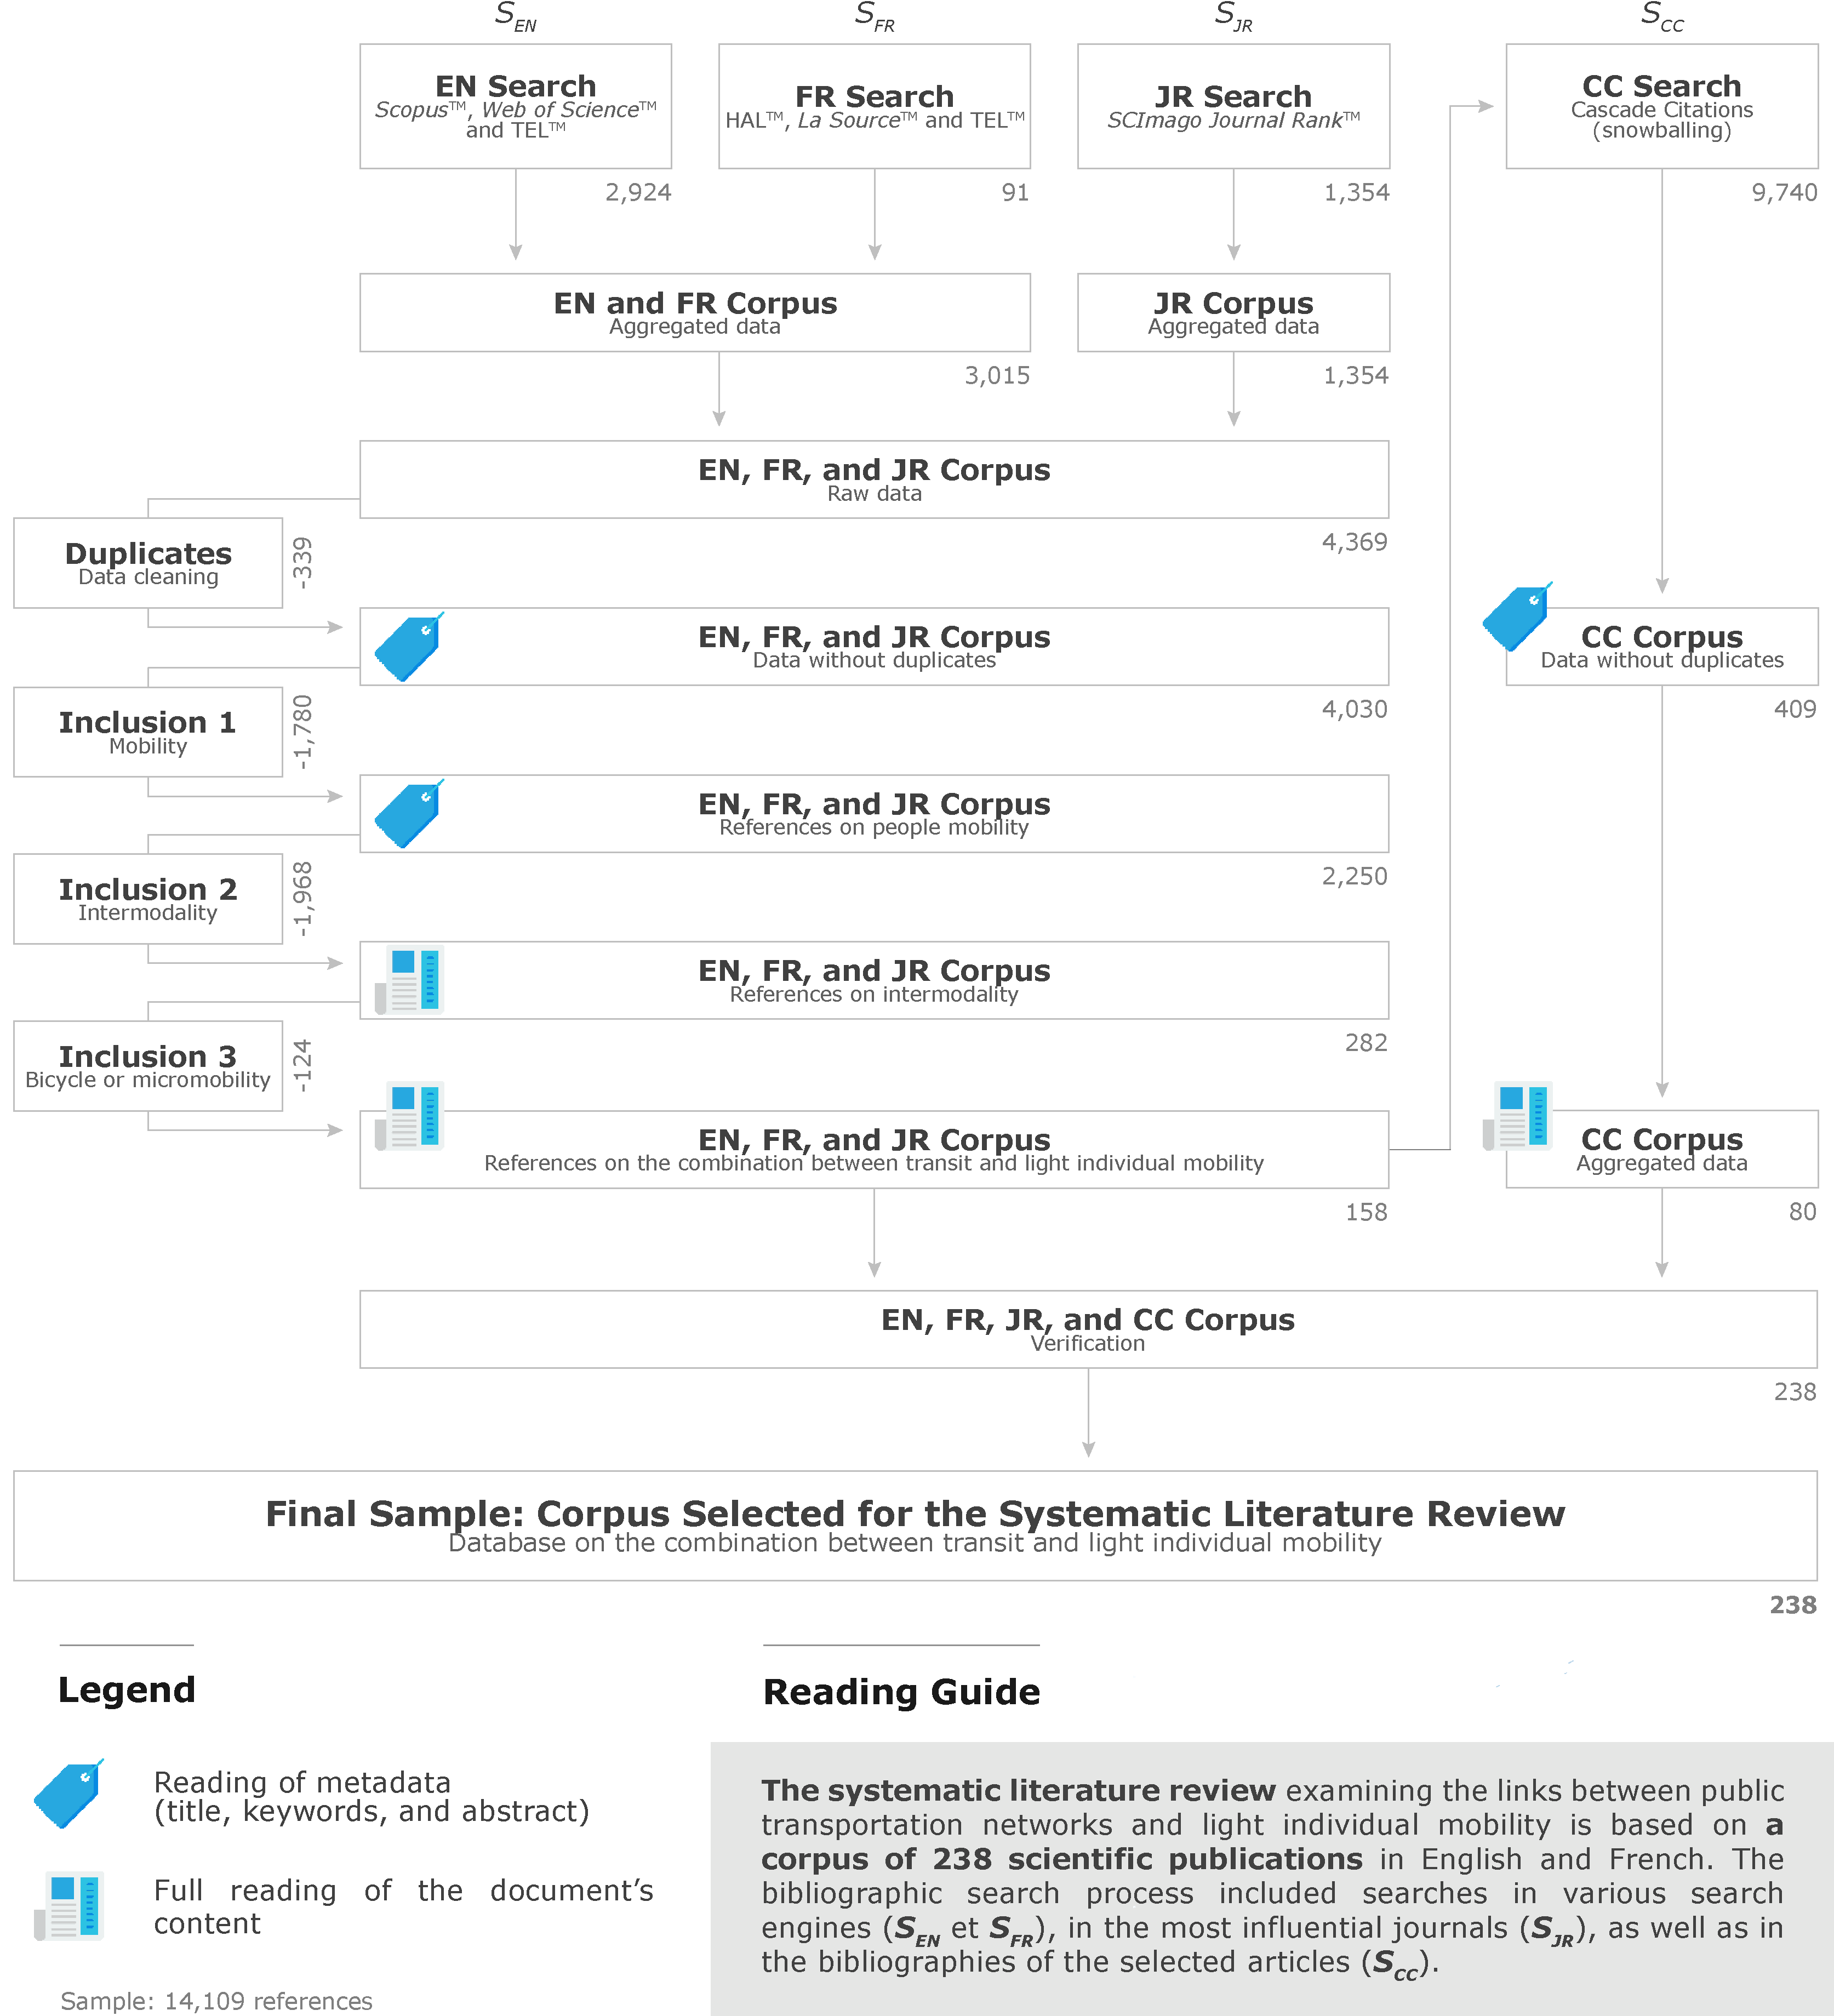
\includegraphics[width=1\columnwidth]{src/Figures/Chap-2/EN_RSL_Diagramme_flux_selection_publications.pdf}}
        \vspace{5pt}
        \begin{flushright}\scriptsize{
        Author: \textcolor{blue}{Dylan Moinse (2023)}
        }\end{flushright}
    \end{figure}

    % Searches EN+FR
In the first case, we queried the \Marque{Scopus} and \Marque{Web of Science} databases\footnote{~
    \textsl{Scopus} (\url{www.scopus.com}) and \textsl{Web of Science} (\url{www.webofscience.com}) are online bibliographic platforms commonly used in academic research. \textsl{Scopus} is developed by \Marque{Elsevier}, a company specializing in scientific publishing, while \textsl{Web of Science} is a collection of academic works managed by \Marque{Clarivate Analytics}.
}. Additionally, the \Marque{TEL} server\footnote{~
    \textsl{theses.fr} (\url{www.theses.fr}) is a platform for doctoral theses, regularly providing online access to academic resources produced by doctoral students.
} was consulted to expand the search to doctoral theses submitted in English. In the second phase, the bibliographic research in French relied on the \Marque{HAL} portal\footnote{~
    \textsl{Hyper Article en Ligne} (\url{https://hal.science/}) is an open archive portal that facilitates the deposit, dissemination, and consultation of scientific documents. This portal was developed by the \acrfull{CCSD} of the \acrfull{CNRS}. \textsl{HAL} allows researchers and institutions to disseminate their research freely to facilitate open access and visibility.
}, the \Marque{La Source} platform\footnote{~
    \textsl{La Source} (\url{https://bibliotheque.enpc.fr}) is the online library developed by the \textsl{École des Ponts Paristech}, designed to facilitate access to scientific resources available on its online platform.
}, and again on the \textsl{TEL} server. The \Commas{\acrshort{EN~Search}} resulted in the compilation of 2,924 scientific publications, while the \Commas{\acrshort{FR~Search}} added 91 references, after updating the collection in April 2023. Thus, this first step of the online search formed a corpus of 3,015 documents, referred to as the \Commas{EN and FR Corpus} (see \hyperref[fig-chap2:diagramme-flux-selection-publications-rsl]{Figure~\ref{fig-chap2:diagramme-flux-selection-publications-rsl}}, page~\pageref{fig-chap2:diagramme-flux-selection-publications-rsl}).%%Translated%%

    % Table scientific journals
% Table of station area types
%%Translated%%
        \begin{table}[h!]
    \centering
    \renewcommand{\arraystretch}{1.5}
    \resizebox{\columnwidth}{!}{
    \begin{tabular}{p{0.07\columnwidth}p{0.1\columnwidth}p{0.7\columnwidth}p{0.13\columnwidth}}
        %\hline
    \rule{0pt}{15pt} \small{\textbf{\textcolor{blue}{Rank}}} & \small{\textbf{\textcolor{blue}{Label}}} & \small{\textbf{\textcolor{blue}{Scientific Journal}}} & \small{\textbf{\textcolor{blue}{\acrshort{SJR} Index}}}\\
        \hline
    \multicolumn{4}{l}{\small{\textbf{\textcolor{blue}{Transport (2023)}}}}\\
\small{1} & \small{\(SMG_{T1}\)} & \small{\textsl{Analytic Methods in Accident Research}} & \small{4.8}\\
\small{2} & \small{\(SMG_{T2}\)} & \small{\textsl{Tourism Management}} & \small{3.4}\\
\small{3} & \small{\(SMG_{T3}\)} & \small{\textsl{Transportation Research Part B: Methodological}} & \small{3.4}\\
\small{4} & \small{\(SMG_{T4}\)} & \small{\textsl{Journal of Travel Research}} & \small{3.3}\\
\small{5} & \small{\(SMG_{T5}\)} & \small{\textsl{Transportation Research Part C: Emerging Technologies}} & \small{3.2}\\
\small{6} & \small{\(SMG_{T6}\)} & \small{\textsl{Transport Reviews}} & \small{3.1}\\
\small{7} & \small{\(SMG_{T7}\)} & \small{\textsl{Transportation Research Part E: Logistics and Transportation}} & \small{2.8}\\
\small{8} & \small{\(SMG_{T8}\)} & \small{\textsl{Transportation Science}} & \small{2.8}\\
\small{9} & \small{\(SMG_{T9}\)} & \small{\textsl{Journal of Public Transportation}} & \small{2.3}\\
\small{10} & \small{\(SMG_{T10}\)} & \small{\textsl{Transportation Research, Part A: Policy and Practice}} & \small{2.2}\\
        \hline
    \multicolumn{4}{l}{\small{\textbf{\textcolor{blue}{Urban Studies (2023)}}}}\\
\small{1} & \small{\(SMG_{U1}\)} & \small{\textsl{Nature Sustainability}} & \small{5.8}\\
\small{2} & \small{\(SMG_{U2}\)} & \small{\textsl{Journal of Urban Economics}} & \small{2.8}\\
\small{3} & \small{\(SMG_{U3}\)} & \small{\textsl{Journal of Public Transportation}} & \small{2.3}\\
\small{4} & \small{\(SMG_{U4}\)} & \small{\textsl{Transportation Research Interdisciplinary Perspectives}} & \small{2.1}\\
\small{5} & \small{\(SMG_{U5}\)} & \small{\textsl{Landscape and Urban Planning}} & \small{1.9}\\
\small{6} & \small{\(SMG_{U6}\)} & \small{\textsl{Urban Studies}} & \small{1.9}\\
\small{7} & \small{\(SMG_{U7}\)} & \small{\textsl{International Journal of Urban and Regional Research}} & \small{1.9}\\
\small{8} & \small{\(SMG_{U8}\)} & \small{\textsl{Journal of the American Planning Association}} & \small{1.8}\\
\small{9} & \small{\(SMG_{U9}\)} & \small{\textsl{Computers, Environment and Urban Systems}} & \small{1.7}\\
\small{10} & \small{\(SMG_{U10}\)} & \small{\textsl{Cities}} & \small{1.7}\\
        \hline
        \end{tabular}}
    \caption{List of scientific journals ranked by the \Marque{SCImago Journal Rank}, included in the \Commas{JR~Search} of the systematic literature review.}
    \label{table-chap2:revues-scientifiques-rsl}
        \vspace{5pt}
        \begin{flushleft}\scriptsize{
        \textcolor{blue}{Note:} The journal \textsl{Journal of Public Transportation} appears in both rankings (\(SMG_{T9}\) and \(SMG_{U3}\)).
        \\
        \textcolor{blue}{Reading:} The twenty most influential transport and urban studies journals were individually reviewed to identify relevant scientific publications related to the topic of our systematic literature review.
        }\end{flushleft}
        \begin{flushright}\scriptsize{
        Data source: \Marque{SCImago Journal Rank}~\textcolor{blue}{\autocite{sjr_scimago_2023}}
        }\end{flushright}
        \end{table}%%Translated%%

    % CR Search
Despite the variety of scientific publications accessible through the aforementioned documentary databases and servers, their advanced search features may prove insufficient to cover the entire field of study, due to constraints in search algorithms and the formulation of the defined keywords. To overcome the limitations of the advanced search tools available in these electronic sources, the search strategy for this \acrshort{SLR} was enhanced by a second stage of bibliographic exploration, involving the direct consultation of peer-reviewed scientific journals. This manual bibliographic search, referred to as \acrfull{JR~Search}, or \(S_{JR}\), follows the method employed by \textcolor{blue}{\textcite[738]{padeiro_transit-oriented_2019}}\index{Padeiro, Miguel|pagebf}\index{Louro, Ana|pagebf}\index{Costa, Nuno Marques de|pagebf}. To this end, we consulted an international classification of scientific journals by discipline, provided by the online platform \textsl{SJR}\footnote{~
    \textsl{SJR} is a platform developed by \Marque{SCImago Lab}, providing several performance indicators to evaluate peer-reviewed journals, notably the \acrfull{SJR} index, which measures the reputation and scientific impact of journals. The \textsl{SJR} tool uses the \Marque{PageRank} algorithm from \Marque{Google} to determine the quality and influence of a journal, considering the number of citations received by each article, the quality of the citing journals, and the relevant scientific disciplines. The \acrshort{SJR} index is an alternative to the \acrfull{h-index} and offers a more nuanced perspective on a journal's impact by considering both the quantity and quality of citations received.
} that established the \acrfull{SJR} index to measure the quality and influence of a journal. Based on this ranking, we found it relevant to consult the top ten scientific journals in the fields of \Commas{transportation} and \Commas{urban studies,} resulting in a \Commas{CR Corpus} of 1,354 publications (see \hyperref[table-chap2:revues-scientifiques-rsl]{Table~\ref{table-chap2:revues-scientifiques-rsl}}, page~\pageref{table-chap2:revues-scientifiques-rsl}). After cleaning the data by removing duplicates and revising in 2023, the \Commas{EN, FR, and CR Corpus} includes a total of 4,030 bibliographic references (see \hyperref[fig-chap2:diagramme-flux-selection-publications-rsl]{Figure~\ref{fig-chap2:diagramme-flux-selection-publications-rsl}}, page~\pageref{fig-chap2:diagramme-flux-selection-publications-rsl}).%%Translated%%

    % 2.1.3.
    \needspace{1\baselineskip} % Reserve space
\subsection{Selection Process of Scientific Publications
    \label{chap2:selection-publications-scientifiques}
    }

    % Table expression
% Search expression table
%%Translated%%
        \begin{table}[h!]
    \centering
    \renewcommand{\arraystretch}{1.5}
    \resizebox{\columnwidth}{!}{
    \begin{tabular}{p{0.5\columnwidth}p{0.5\columnwidth}}
        %\hline
    \rule{0pt}{15pt} \small{\textbf{\textcolor{blue}{\acrshort{EN~Search}}}} & \small{\textbf{\textcolor{blue}{\acrshort{FR~Search}}}}\\
        \hline
    \multicolumn{2}{l}{\small{\textbf{\textcolor{blue}{Dimension related to public transport}}}}\\
\small{all=(\textbf{\Commas{\textsl{Transit-Oriented Development}}} or \textbf{\Commas{\textsl{Public Transport}}} or \textbf{\Commas{\textsl{Transit}}} or \textbf{\Commas{\textsl{Rail}}} or \textbf{\Commas{\textsl{Train}}} or \textbf{\Commas{\textsl{Metro}}} or \textbf{\Commas{\textsl{Tram}}} or \textbf{\Commas{\textsl{Bus}}})} & \small{all=(\textbf{\Commas{\textsl{Transit-Oriented Development}}} or \textbf{\Commas{\textsl{Urbanisme orienté}}} or \textbf{\Commas{\textsl{Public Transport}}} or \textbf{\Commas{\textsl{Collective Transport}}} or \textbf{\Commas{\textsl{Rail}}} or \textbf{\Commas{\textsl{Train}}} or \textbf{\Commas{\textsl{Railway}}} or \textbf{\Commas{\textsl{Metro}}} or \textbf{\Commas{\textsl{Tram}}} or \textbf{\Commas{\textsl{BRT}}} or \textbf{\Commas{\textsl{Bus}}})}\\
        \hdashline
    \multicolumn{2}{l}{\small{\textbf{\textcolor{blue}{Boolean Operator}}}}\\
 \multicolumn{2}{l}{\small{and}}\\
        \hdashline
    \multicolumn{2}{l}{\small{\textbf{\textcolor{blue}{Dimension related to light individual mobility}}}}\\
\small{all=(\textbf{\Commas{\textsl{Micromobility}}} or \textbf{\Commas{\textsl{Micro-Mobility}}} or \textbf{\Commas{\textsl{Bicycle*}}} or \textbf{\Commas{\textsl{Bike*}}} or \textbf{\Commas{\textsl{Bike-And-Ride}}} or \textbf{\Commas{\textsl{Cycling}}} or \textbf{\Commas{\textsl{E-Scooter*}}} or \textbf{\Commas{\textsl{Scooter*}}} or \textbf{\Commas{\textsl{Device*}}})} & \small{all=(\textbf{\Commas{\textsl{Micro-mobility*}}} or \textbf{\Commas{\textsl{Micromobility*}}} or \textbf{\Commas{\textsl{Bicycle*}}} or \textbf{\Commas{\textsl{Bike*}}} or \textbf{\Commas{\textsl{Active Mode*}}} or \textbf{\Commas{\textsl{Soft Mode}}} or \textbf{\Commas{\textsl{Cycle*}}} or \textbf{\Commas{\textsl{Cyclable}}} or \textbf{\Commas{\textsl{Scooter*}}} or \textbf{\Commas{\textsl{Micro-vehicle*}}})}\\
        \hdashline
    \multicolumn{2}{l}{\small{\textbf{\textcolor{blue}{Boolean Operator}}}}\\
\multicolumn{2}{l}{\small{and}}\\
        \hdashline
    \multicolumn{2}{l}{\small{\textbf{\textcolor{blue}{Dimension related to intermodality-passenger(s)}}}}\\
\small{all=(\textbf{\Commas{\textsl{Intermodal*}}} or \textbf{\Commas{\textsl{Combination}}} or \textbf{\Commas{\textsl{*Last Mile}}} or \textbf{\Commas{\textsl{First Mile*}}} or \textbf{\Commas{\textsl{FLM}}} or \textbf{\Commas{\textsl{Feeder}}} or \textbf{\Commas{\textsl{Transfer}}} or \textbf{\Commas{\textsl{Relation*}}} or \textbf{\Commas{\textsl{Integration}}} or \textbf{\Commas{\textsl{Catchment}}} or \textbf{\Commas{\textsl{Isochrone*}}} or \textbf{\Commas{\textsl{Buffer}}} or \textbf{\Commas{\textsl{Service Coverage}}} or \textbf{\Commas{\textsl{Shed*}}} or \textbf{\Commas{\textsl{Station Area*}}} or \textbf{\Commas{\textsl{Access}}} or \textbf{\Commas{\textsl{Egress}}})} & \small{all=(\textbf{\Commas{\textsl{Intermodal*}}} or \textbf{\Commas{\textsl{Combination}}} or \textbf{\Commas{\textsl{First* Mile*}}} or \textbf{\Commas{\textsl{Last* Mile*}}} or \textbf{\Commas{\textsl{Feeder}}} or \textbf{\Commas{\textsl{Pre-access}}} or \textbf{\Commas{\textsl{Diffusion}}} or \textbf{\Commas{\textsl{Post-access}}} or \textbf{\Commas{\textsl{Interaction*}}} or \textbf{\Commas{\textsl{Integration}}} or \textbf{\Commas{\textsl{Catchment Area}}} or \textbf{\Commas{\textsl{Influence Area}}} or \textbf{\Commas{\textsl{Isochrone*}}} or \textbf{\Commas{\textsl{Station Area*}}})}\\
        \hline
        \end{tabular}}
    \caption{Search expression of keywords in English and French, covering three thematic categories, for the systematic literature review.}
    \label{table-chap2:expression-recherche-rsl}
        \vspace{5pt}
        \begin{flushleft}\scriptsize{
        \textcolor{blue}{Note:} The asterisk (*) provides greater flexibility to terms by allowing a wider scope in advanced searches, accommodating additional characters before or after the word. As a result, this symbol includes plural forms or variants of terms, among other possibilities.
        \\
        \textcolor{blue}{Reading:} The bibliographic search formula relies on three conditions: lexical presence referring to public transport, light individual mobility, and intermodality.
        }\end{flushleft}
        \begin{flushright}\scriptsize{
        Author: \textcolor{blue}{Dylan Moinse (2023)}
        }\end{flushright}
        \end{table}%%Translated%%

    % Boolean operators
The identification of academic works related to \acrshort{M-TOD} was carried out by using the specified electronic databases. A search expression was defined based on three distinct categories, namely public transport (i), light individual mobility (ii), and intermodal travel (iii). Considering the terminological variations of each category, the expression was enhanced with the integration of boolean operators \Commas{and} (\textsl{and}) and \Commas{or} (\textsl{or}) to cover the three classes of keywords (see \hyperref[table-chap2:expression-recherche-rsl]{Table~\ref{table-chap2:expression-recherche-rsl}}, page~\pageref{table-chap2:expression-recherche-rsl}). The designation of keywords was facilitated by a preliminary reading phase, which allowed us to identify recurring terms, thus strengthening the robustness of the expression. It should be noted that the terms in each incorporated group in the formula were considered synonyms, requiring the actual presence of at least one word from each category for a publication to be included in the search results. The integrated tools of the advanced search were used and configured to probe the content of scientific publications, except for the \textsl{TEL} server, where we performed a manual search.%%Translated%%

    % Inclusion criteria
After the collection and cleaning of the data, the next step towards building a corpus of scientific publications on \acrshort{M-TOD} involves excluding documents that do not pertain to this research topic. To be considered eligible, studies must meet five predetermined inclusion criteria:
    \begin{customitemize}
        \item The full content of the document is available online;
        \item The publication is written in English or French;
        \item The document focuses on human mobility;
        \item The scientific work is focused on intermodal travel;
        \item The main subject of study concerns the integration of light individual mobility into public transport systems.
    \end{customitemize}%%Translated%%

    % Inclusion process
The evaluation of the relevance of the documents was implemented through cross-reading. By examining the metadata of the scientific publications, we first filtered the bibliographic database based on the language of writing and the field of study. The reduction of the initial collection to only those research works focusing on human mobility led to a list of 2,250 bibliographic references. For this, we retained only those publications whose content includes the term \Commas{mobility} (\textsl{mobility}) at least once. The selection process was then refined by exclusively integrating documents related to the combination of light individual mobility and public transport, through a detailed examination of their content. The repository was thus narrowed down to a corpus of 158 documents (see \hyperref[fig-chap2:diagramme-flux-selection-publications-rsl]{Figure~\ref{fig-chap2:diagramme-flux-selection-publications-rsl}}, page~\pageref{fig-chap2:diagramme-flux-selection-publications-rsl}). The exclusion of a scientific publication from the final corpus was systematically accompanied by a justification based on the defined inclusion criteria. Following the application of the non-selection conditions, the resulting \Commas{Corpus EN, FR and CR} went through a validation process, during which each of the 158 documents was reviewed to ensure its compliance with the research topic of the \acrshort{SLR}.%%Translated%%

    % Cascade citations
Once the \Commas{Corpus EN, FR and CR} was established, it was supplemented by a final bibliographic collection step from the 158 included scientific publications, called \acrfull{CC~Search}, or \(S_{CC}\). During this phase, the focus was placed on exploring the citations contained within the bibliographies listed in the entire document collection to minimize the omission of scientific publications. This approach, known as the \Commas{snowball effect} \textcolor{blue}{\autocite[2545]{jain_systematic_2020}}\index{Jain, Deepshikha|pagebf}\index{Singh, Ekta|pagebf}\index{Ashtt, Rashmi|pagebf}, led to the inclusion of 80 new unique bibliographic references that met the requirements. In summary, the successive bibliographic searches conducted on English-language portals (\Commas{\acrshort{EN~Search}}), French-language portals (\Commas{\acrshort{FR~Search}}), several scientific journals (\Commas{JR~Search}), and from the collected bibliographies (\Commas{CC~Search}), the \acrshort{SLR} on \acrshort{M-TOD} is based on a \Commas{Corpus EN, FR, CR and CC} of 238 scientific publications, forming the material deployed in this chapter (see \hyperref[fig-chap2:diagramme-flux-selection-publications-rsl]{Figure~\ref{fig-chap2:diagramme-flux-selection-publications-rsl}}, page~\pageref{fig-chap2:diagramme-flux-selection-publications-rsl}).%%Translated%%

    % 2.1.4.
    \needspace{1\baselineskip} % Reserve space
\subsection{Data Extraction and Aspects Considered
    \label{chap2:extraction-donnees-aspects-consideres}
    }
    
    % Extraction and analysis
The thematic approach of this \acrshort{SLR} adopts the format of a critical and synthetic reading exercise, with data extraction and management facilitated by the bibliographic management software \Marque{Zotero} and the spreadsheet \Marque{Excel}. In addition to its functionalities for calculation, data analysis, programming, and graphical representation, \textsl{Excel} helps organize the collected information while providing a comprehensive and tailored overview for the practice of \acrshort{SLR}. In this regard, this tool facilitates sorting and filtering the data according to specific criteria, as well as performing statistical and qualitative analyses that can be integrated with other research tools. Given the moderate volume of bibliographic data, we favored \textsl{Excel} for the literature review analysis, compared to more advanced programming tools such as \Marque{MySQL} or \Marque{Python}.%%Translated%%

    % Table of studied aspects
% Table of studied aspects
%%Translated%%
        \begin{table}[h!]
    \centering
    \renewcommand{\arraystretch}{1.5}
    \resizebox{\columnwidth}{!}{
    \begin{tabular}{p{0.5\columnwidth}p{0.5\columnwidth}}
        %\hline
    \rule{0pt}{15pt} \small{\textbf{\textcolor{blue}{Studied Aspects}}} & \small{\textbf{\textcolor{blue}{Sub-sections}}}\\
        \hline
    \multicolumn{2}{l}{\small{\textbf{\textcolor{blue}{Metadata and Networks}}}}\\
\small{Author(s), institutions, scientific journals, citations} & \small{\hyperref[chap2:etat-litterature-scientifique-internationale-btod]{sub-section 2.1} (page~\pageref{chap2:etat-litterature-scientifique-internationale-btod})}\\
    \hdashline
    \multicolumn{2}{l}{\small{\textbf{\textcolor{blue}{Terminology}}}}\\
\small{Title, keywords, abstract, content} & \small{\hyperref[chap2:analyse-textuelle]{sub-section 2.1.2} (page~\pageref{chap2:analyse-textuelle})}\\
    \hdashline
    \multicolumn{2}{l}{\small{\textbf{\textcolor{blue}{Study Objects}}}}\\
\small{light individual mobility, public transport, forms of intermodal integration} & \small{\hyperref[chap2:evolution-recherches-tc-mobilite-individuelle-legere]{sub-section 2.1.3} (page~\pageref{chap2:evolution-recherches-tc-mobilite-individuelle-legere})}\\
    \hdashline
    \multicolumn{2}{l}{\small{\textbf{\textcolor{blue}{Geographical Areas}}}}\\
\small{Case studies, geographical scales, international comparisons} & \small{\hyperref[chap2:exploration-terrains-geographiques]{sub-section 2.1.4} (page~\pageref{chap2:exploration-terrains-geographiques})}\\
    \hdashline
    \multicolumn{2}{l}{\small{\textbf{\textcolor{blue}{Concepts}}}}\\
\small{Theoretical frameworks, place of \acrshort{TOD}} & \small{\hyperref[chap2:fondements-theoriques]{sub-section 2.2.1} (page~\pageref{chap2:fondements-theoriques})}\\
    \hdashline
    \multicolumn{2}{l}{\small{\textbf{\textcolor{blue}{Methodology}}}}\\
\small{Research methods, data sources, sampling, types of analysis} & \small{\hyperref[chap2:methodes-collecte-donnees]{sub-sections 2.2.2} and \hyperref[chap2:demarches-types-analyses]{2.2.3} (pages \pageref{chap2:methodes-collecte-donnees} and \pageref{chap2:demarches-types-analyses})}\\
    \hdashline
    \multicolumn{2}{l}{\small{\textbf{\textcolor{blue}{TOD Principles (\Commas{\acrshort{7Ds}})}}}}\\
\small{Density, diversity, design, accessibility of destinations, distance to public transport stations, demand management, and social inclusion} & \small{\hyperref[chap2:densite-population]{sub-sections 3.1} (page~\pageref{chap2:densite-population}), \hyperref[chap2:diversite-fonctionnelle]{3.2} (page~\pageref{chap2:diversite-fonctionnelle}), \hyperref[chap2:traitement-espaces-publics]{3.3} (page~\pageref{chap2:traitement-espaces-publics}), \hyperref[chap2:accessibilite-intermodale]{3.4} (page~\pageref{chap2:accessibilite-intermodale}), \hyperref[chap2:distances-premiers-derniers-km]{3.5} (page~\pageref{chap2:distances-premiers-derniers-km}), \hyperref[chap2:gestion-demande-mobilite]{3.6} (page~\pageref{chap2:gestion-demande-mobilite}) and \hyperref[chap2:sociodemographie-usagers]{3.7} (page~\pageref{chap2:sociodemographie-usagers})}\\
    \hdashline
    \multicolumn{2}{l}{\small{\textbf{\textcolor{blue}{Mobility Behaviors}}}}\\
\small{Reasons, experience, social representations} & \small{\hyperref[chap2:comportements-mobilite]{sub-section 3.8} (page~\pageref{chap2:comportements-mobilite})}\\
    \hdashline
    \multicolumn{2}{l}{\small{\textbf{\textcolor{blue}{Impacts}}}}\\
\small{Mobility, urban planning, economy, environment} & \small{\hyperref[chap2:impacts-systemes-urbain-mobilite]{sub-section 3.9} (page~\pageref{chap2:impacts-systemes-urbain-mobilite})}\\
        \hline
        \end{tabular}}
    \caption{Analysis grid of the systematic literature review on a \textsl{Micromobility-friendly Transit-Oriented Development}.}
    \label{table-chap2:aspects-etudies-rsl}
        \vspace{5pt}
        \begin{flushleft}\scriptsize{
        \textcolor{blue}{Note:} The aspects examined are not confined to a single theme and appear throughout the chapter.
        \\
        \textcolor{blue}{Reading:} The systematic literature review on a transit-oriented urbanism supported by light individual mobility is based on metadata, terminology, study objects, geographical contexts, concepts and techniques mobilized, planning model principles, mobility behaviors, and observed impacts.
        }\end{flushleft}
        \begin{flushright}\scriptsize{
        Author: \textcolor{blue}{Dylan Moinse (2023)}
        }\end{flushright}
        \end{table}%%Translated%%

    % Comparative RSL
In exploring the central axes of \acrshort{M-TOD}, this \acrshort{SLR} follows a perspective similar to the literature review produced by \textcolor{blue}{\textcite[5]{oeschger_micromobility_2020}}\index{Oeschger, Giulia|pagebf}\index{Carroll, Páraic|pagebf}\index{Caulfield, Brian|pagebf} entitled \foreignlanguage{english}{\textsl{Micromobility and Public Transport Integration: The Current State of Knowledge}} in the journal \foreignlanguage{english}{\textsl{Transportation Research Part D: Transport and Environment}}, which thematically synthesizes the integration of bicycles and micromobility into public transport systems. However, the analytical framework adopted in the present \acrshort{SLR} aims to capture the dominant aspects of the urban model while seeking to overcome several limitations identified in the cited literature review. Although the bibliographic synthesis published by researchers from the Department of Engineering at \acrfull{UCD} and \textsl{Trinity College Dublin} manages to intelligibly and concisely aggregate the scientific knowledge regarding the connections between light individual mobility and public transport, this scientific article faces a notable underrepresentation of the European continent. This can largely be explained by language barriers, which are reflected in its relatively limited collection of articles. Additionally, the territorial lens of this modal combination is less central, and the electric scooter, whose rise was still nascent, is only marginally present. In the following sections of this chapter, we will discuss the results from the thematic analysis of this academic corpus, spanning the time range from 1993 to 2023, dedicated to the characterization of \acrshort{M-TOD}.%%Translated%%

    % Dimensions M-TOD
The analysis framework developed to examine the \acrshort{M-TOD} through this \acrshort{SLR} reflects the fundamentals of the urban model under scrutiny. Our attention is directed toward the existing interactions between intermodal integration, territorial design, socio-economic and environmental impacts, mobility behaviors, governance models, the internationalization of \acrshort{M-TOD}, and the challenges that arise in the conceptualization and application of this urban strategy (see \hyperref[table-chap2:aspects-etudies-rsl]{Table~\ref{table-chap2:aspects-etudies-rsl}}, page~\pageref{table-chap2:aspects-etudies-rsl}).%%Translated%%

    % ___________________________________________
    % 2.2.
    \newpage
    \needspace{1\baselineskip} % Reserve space
    \sectionheader{Meta-analysis of the bibliographic corpus on the M-TOD}
\section{Analysis of the Documentation Integrated into the Systematic Literature Review
    \label{chap2:analyse-documentation-rsl}
    }

    % Introduction
The presentation of the results, deployed in a multidimensional manner in this section, serves as a true exercise in conciseness by providing an overview that encompasses the complexity and diversity of the issues surrounding the urban model. Simultaneously, this \acrshort{SLR} mobilizes a dense corpus of scientific publications, enabling us to combine both quantitative and qualitative analyses of the issues and dynamics associated with the definition of \acrshort{M-TOD}. The exploitation of the constructed bibliographic database thus informs the scientific reflections of this doctoral thesis, serving as a key reference to guide, subsequently, the investigation conducted primarily in the Hauts-de-France region.%%Translated%%

    % Annonce du plan 1
This section aims to describe the main results emerging from the \acrshort{SLR} as follows. First, \hyperref[chap2:etat-litterature-scientifique-internationale-btod]{Subsection~\ref{chap2:etat-litterature-scientifique-internationale-btod}} (page~\pageref{chap2:etat-litterature-scientifique-internationale-btod}) explores the state of the scientific literature on \acrshort{M-TOD}, combining a \hyperref[chap2:analyse-bibliometrique]{bibliometric analysis} (page~\pageref{chap2:analyse-bibliometrique}) of the mobilized corpus, an analysis of the \hyperref[chap2:analyse-textuelle]{terminology used} (page~\pageref{chap2:analyse-textuelle}) to describe the research topic, as well as the \hyperref[chap2:evolution-recherches-tc-mobilite-individuelle-legere]{temporal} (page~\pageref{chap2:evolution-recherches-tc-mobilite-individuelle-legere}) and \hyperref[chap2:exploration-terrains-geographiques]{geographical} (page~\pageref{chap2:exploration-terrains-geographiques}) aspects of the scientific publications integrated into the \acrshort{SLR}.%%Translated%%

    % Annonce du plan 2
The second section, presented in \hyperref[chap2:cadres-conceptuels-methodologiques]{Subsection~\ref{chap2:cadres-conceptuels-methodologiques}} (page~\pageref{chap2:cadres-conceptuels-methodologiques}), details the conceptual and methodological frameworks, structured around a description of the \hyperref[chap2:fondements-theoriques]{theoretical framework} (page~\pageref{chap2:fondements-theoriques}), the \hyperref[chap2:methodes-collecte-donnees]{research methods} (page~\pageref{chap2:methodes-collecte-donnees}), and the \hyperref[chap2:demarches-types-analyses]{analytical approaches} used to capture \acrshort{M-TOD} (page~\pageref{chap2:demarches-types-analyses}).%%Translated%%

    % 2.2.1. authors, textual analysis, chronology, MM+Transit types, case studies
    \needspace{1\baselineskip} % Reserve space
\subsection{State of the International Scientific Literature on \textsl{Micromobility-friendly Transit-Oriented Development}
    \label{chap2:etat-litterature-scientifique-internationale-btod}
    }
    
    % Introduction
The initial phase of the analysis is dedicated to examining the metadata of the scientific publications collected as part of the \acrshort{SLR} in order to gain a better understanding of the research practices. The following questions guide the analysis of the scientific literature devoted to studying \acrshort{M-TOD}:
    \begin{customitemize}
        \item What are the existing networks within this English and French academic corpus, such as interconnections and collaborations between authors, institutions, and scientific journals?
        \item Can we identify lexical patterns revealing the existence of practices, trends, or even specific norms related to the subjects studied?
        \item From a temporal perspective, how do these studies relate to a dynamic research topic?
        \item Regarding the spatial dimension of the analyzed corpus, does the selection of the studied sites represent a concentration of geographical contexts within the same region?
    \end{customitemize}%%Translated%%

    % 2.2.1.1. Interconnection networks, scientific journals, institutions
    \needspace{1\baselineskip} % Reserve space
\subsubsection*{Bibliometric Analysis of the Academic Corpus
    \label{chap2:analyse-bibliometrique}
    }

    % Languages and document types
The studied corpus consists of 238 bibliographic references, of which 228 sources are published in English and 10 publications in French. Peer-reviewed scientific articles, totaling 204 publications, predominate among the documents selected for analysis. In parallel, the document collection includes 13 research reports, 12 conference proceedings, four book chapters, four master's theses, and one doctoral dissertation. It is worth noting that 88\% of the English-language publications are scientific articles, while among the ten French-language documents, only three are categorized as scientific articles.%%Translated%%

    % Occurrences of authors
The examination of metadata led to an investigation of the \Commas{productivity} of authors in relation to the selected publications, providing an overview of multidisciplinary collaborations and mutual influences within the scientific community contributing to this specific research field. Various conceptual, intellectual, and social visualization techniques \textcolor{blue}{\autocite[559]{fortuna_global_2020}}\index{Fortuna, Giulio|pagebf}\index{Aria, Massimo|pagebf}\index{Iorio, Carmela|pagebf}\index{Mignogna, Michele~D.|pagebf}\index{Klasser, Gary~D.|pagebf} were used to analyze the knowledge structures examined in this section, referring to the visual representations adapted for \acrshort{HSS} by \textcolor{blue}{\textcite[94-97]{ballouk_analyse_2021}}\index{Ballouk, Houssein|pagebf}\index{Ben Jabeur, Sami|pagebf}\index{Ben Arfi, Wissal|pagebf}. In accordance with \hyperref[fig-chap2:interconnexions-auteurs-rsl]{Figure~\ref{fig-chap2:interconnexions-auteurs-rsl}} (page~\pageref{fig-chap2:interconnexions-auteurs-rsl}) in the form of a heatmap\footnote{~
    As the hue approaches purple, the concentration of authors intensifies. This density map provides an overview of the research structure centered around this topic, highlighting not only the contribution of authors quantitatively but also their interactions through co-publications.
}, this visual representation highlights the observation of four predominant co-author clusters, mainly centered around \textcolor{blue}{Lissy La Paix Puello}, \textcolor{blue}{Niels van Oort}, \textcolor{blue}{Yanjie Ji}, and \textcolor{blue}{Hang Wei}. The analysis of the occurrences of contributors within the academic corpus notably brings to the forefront the significant presence of researchers affiliated with institutions in the Netherlands, the United States, and China.
    \begin{customitemize}
    % Lissy La Paix Puello
        \item \textcolor{blue}{Lissy La Paix Puello} is a Lecturer and \textcolor{blue}{Karst Geurs} is a Professor, both at the Department of Civil Engineering at the University of Twente (Netherlands). These researchers are referenced in six bibliographic sources integrated into the \acrshort{SLR}, exploring the modal choice of cycling to access train stations \textcolor{blue}{\autocite{la_paix_puello_modelling_2015,la_paix_puello_train_2016}}\index{La Paix Puello, Lissy|pagebf}\index{Geurs, Karst~T.|pagebf}, measuring a cost index related to cycling access to train stations \textcolor{blue}{\autocite{la_paix_puello_integration_2016}}\index{La Paix Puello, Lissy|pagebf}\index{Geurs, Karst~T.|pagebf}, evaluating the quality of cycling infrastructure around train stations \textcolor{blue}{\autocite{la_paix_puello_role_2021}}\index{La Paix Puello, Lissy|pagebf}\index{Cherchi, Elisabetta|pagebf}\index{Geurs, Karst~T.|pagebf}, examining the potential for cycling access to public transport networks \textcolor{blue}{\autocite{souza_modelling_2017}}\index{Souza, Flavia de|pagebf}\index{La Paix Puello, Lissy|pagebf}\index{Brussel, Mark|pagebf}\index{Orrico, Romulo|pagebf} and studying the impact of cycling and public transport integration policies on network ridership and access to employment \textcolor{blue}{\autocite{geurs_multi-modal_2016}}\index{Geurs, Karst~T.|pagebf}\index{La Paix Puello, Lissy|pagebf}\index{Weperen, Sander van|pagebf};
    % Niels van Oort
        \item \textcolor{blue}{Niels van Oort} is a Professor at the Delft University of Technology (Netherlands). Appearing as an author or co-author in six scientific publications included in the corpus, he conducts research in the fields of multimodal network modeling integrating cycling and bus \textcolor{blue}{\autocite{brand_modelling_2017}}\index{Brand, Judith Caroline|pagebf}\index{Hoogendoorn, Serge|pagebf}\index{Oort, Niels van|pagebf}\index{Schalkwijk, Bart|pagebf} or cycling and tram \textcolor{blue}{\autocite{rijsman_walking_2019}}\index{Rijsman, Lotte|pagebf}\index{Oort, Niels van|pagebf}\index{Ton, Danique|pagebf}\index{Hoogendoorn, Serge|pagebf}\index{Molin, Eric|pagebf}\index{Teijl, Thomas|pagebf}, modal choice for access to train stations \textcolor{blue}{\autocite{shelat_analysing_2018}}\index{Shelat, Sanmay|pagebf}\index{Huisman, Raymond|pagebf}\index{Oort, Niels van|pagebf}, factors influencing these intermodal practices \textcolor{blue}{\autocite{ton_understanding_2020}}\index{Ton, Danique|pagebf}\index{Shelat, Sanmay|pagebf}\index{Nijënstein, Sandra|pagebf}\index{Rijsman, Lotte|pagebf}\index{Oort, Niels van|pagebf}\index{Hoogendoorn, Serge|pagebf} and analysis of user profiles \textcolor{blue}{\autocites{mil_insights_2020}{kuijk_preferences_2022}}\index{Mil, Joeri~F.P. van|pagebf}\index{Leferink, Tessa~S.|pagebf}\index{Annema, Jan Anne|pagebf}\index{Oort, Niels van|pagebf}\index{Kuijk, Roy~J. van|pagebf}\index{Almeida Correia, Gonçalo Homem de|pagebf}\index{Oort, Niels van|pagebf}\index{Arem, Bart van|pagebf};
    % Yanjie Ji
        \item \textcolor{blue}{Yanjie Ji} is a Full Professor at Southeast University (China). Present in five bibliographic references, this researcher studies intermodal user groups using personal bikes or bike-sharing systems \textcolor{blue}{\autocite{ji_public_2017}}\index{Ji, Yanjie|pagebf}\index{Fan, Yingling|pagebf}\index{Ermagun, Alizera|pagebf}\index{Cao, Xuening|pagebf}\index{Wang, Wei|pagebf}\index{Das, Kirti|pagebf}, factors associated with this form of intermodality \textcolor{blue}{\autocite{ji_exploring_2018, liu_use_2020, liu_understanding_2020}}\index{Ji, Yanjie|pagebf}\index{Ma, Xinwei|pagebf}\index{Yang, Mingyuan|pagebf}\index{Jin, Yuchuan|pagebf}\index{Gao, Liangpeng|pagebf}\index{Liu, Yang|pagebf}\index{Feng, Tao|pagebf}\index{Ji, Yanjie|pagebf}\index{Shi, Zhuangbin|pagebf}\index{Ji, Yanjie|pagebf}\index{Feng, Tao|pagebf}\index{Timmermans, Harry~J.~P.|pagebf} and co-developed a method to identify such intermodal trips from smart card data \textcolor{blue}{\autocite{ma_understanding_2018}}\index{Ma, Xinwei|pagebf}\index{Ji, Yanjie|pagebf}\index{Yang, Mingyuan|pagebf}\index{Jin, Yuchuan|pagebf}\index{Tan, Xu|pagebf};
    % Wei Hang & Ting Zuo
        \item \textcolor{blue}{Wei Hang}, then Professor at the Department of Transport Engineering at the University of Cincinnati (USA), and \textcolor{blue}{Ting Zuo}, PhD and transport programmer at the \textsl{Regional Government Council} (USA), participated in the publication of five scientific articles. Their research focuses on the connectivity of \Commas{low-stress bicycle networks} integrated into public transport systems \textcolor{blue}{\autocite{zuo_bikeway_2019, zuo_incorporating_2021}}\index{Zuo, Ting|pagebf}\index{Wei, Heng|pagebf}\index{Chen, Na|pagebf}, on intermodal accessibility models \textcolor{blue}{\autocite{zuo_promote_2020}}\index{Zuo, Ting|pagebf}\index{Wei, Heng|pagebf}\index{Chen, Na|pagebf} using \acrfull{GPS} data \textcolor{blue}{\autocite{zuo_determining_2018}}\index{Zuo, Ting|pagebf}\index{Wei, Hang|pagebf}\index{Rohne, Andrew|pagebf} and on the links between these intermodal practices and equity \textcolor{blue}{\autocite{zuo_first-and-last_2020}}\index{Zuo, Ting|pagebf}\index{Wei, Heng|pagebf}\index{Chen, Na|pagebf}\index{Zhang, Chun|pagebf}.
    \end{customitemize}%%Translated%%

    % French authors
This ranking also highlights several French authors. However, it may be biased due to the preferential inclusion of research written in French. This preferential treatment may have led to the unintentional exclusion of a number of studies written in the national language.%%Translated%%

    % Figure author interconnections
    \begin{figure}[h!]\vspace*{4pt}
        \caption{Interconnections between authors in each of the scientific publications integrated into the systematic review of the literature.}
        \label{fig-chap2:interconnexions-auteurs-rsl}
        \centerline{\includegraphics[width=1\columnwidth]{src/Figures/Chap-2/EN_RSL_Interconnexions_auteurs.png}}
        \vspace{5pt}
        \begin{flushright}\scriptsize{
        Author: \textcolor{blue}{Dylan Moinse (2023)}
        }\end{flushright}
    \end{figure}

    % Author collaborations
The analysis of co-author networks in the \acrshort{SLR} reveals a predominant occurrence of internal connections between the same researchers, suggesting a certain continuity of collaborations across publications (see \hyperref[fig-chap2:interconnexions-auteurs-rsl]{Figure~\ref{fig-chap2:interconnexions-auteurs-rsl}}, page~\pageref{fig-chap2:interconnexions-auteurs-rsl}). However, these microsystems present limited relationships, meaning that the various partnerships within the same scientific community can be seen as somewhat insular with respect to other actors. This phenomenon is also observable when looking at the publication dates visible on the heatmap, with periods showing weak interrelations. It is important to highlight the existence of more developed and open author collaboration networks for the more recent publications.%%Translated%%

    % Scientific Journals
The issue of scientific networks underpins the context in which scientific publications are discussed and made visible. By paying particular attention to the most represented scientific journals within the analysis corpus, we can identify a notable concentration of several renowned international journals. Indeed, the five most influential peer-reviewed journals according to the sample cover 41\% of the bibliographic references, or 84 scientific articles among the 204 included in the \acrshort{SLR}. The top ten journals together account for 58\%. Thus, the journals standing out in the ranking are the \textsl{Transportation Research Record} with 23 publications identified on the \acrshort{M-TOD}, followed by the \textsl{Journal of Transport Geography} with 17 articles, \foreignlanguage{english}{\textsl{Transportation Research Part D: Transport and Environment}} and \foreignlanguage{english}{\textsl{Transportation Research Part A: Policy and Practice}} with 16 articles each, and finally \textsl{Sustainability} with 12 articles. It should be noted that, except for the \textsl{Transportation Research Part A} journal, the journals mentioned did not benefit from the \Commas{JR~Search} step, which involved identifying further publications related to \acrshort{M-TOD} within the most influential journals. This further emphasizes, at the same time, the large diversity of scientific journals present in the corpus, with a total of 83 distinct journals. This plurality is also reflected in the multidisciplinary coverage of the scientific journals. According to data from \Marque{SCImago}, the categories related to \Commas{transport}, \Commas{geography and urbanism}, and \Commas{engineering and civil engineering} hold a predominant place.%%Translated%%

    % Number of citations (h-index)
By taking a closer look at the visibility and valuation of the works within the scientific community, the study of \acrshort{M-TOD} through this \acrshort{SLR} relied on the number of citations received for each of the analyzed works. Among the 204 scientific publications, 26 of them reach the threshold of one hundred citations by peers, while the top ten exceed 200 citations. While the average number of citations is 51, the median of the series is around 22 citations per paper, highlighting significant citation contrasts within the corpus. By looking at the publication year of each document, it can be observed that the ten most cited studies are prior to 2014, and on average, publications with more than one hundred citations date from 2011, compared to the year 2019 for the other 200 publications. The journals most represented among the highly cited articles are primarily \foreignlanguage{english}{\textsl{Transportation Research Part A: Policy and Practice}}, \textsl{Transportation Research Record}, \foreignlanguage{english}{\textsl{Transportation Research Part D: Transport and Environment}}, \textsl{Transport Policy}, and \textsl{Journal of Public Transportation}. The most cited research papers are as follows:
    \begin{customitemize}
\item The scientific article \foreignlanguage{english}{\textsl{Promoting Bike-and-Ride: The Dutch Experience}}, by \textcolor{blue}{Karel} \textcolor{blue}{\textcite[328, 330, 335]{martens_promoting_2007}}\index{Martens, Karel|pagebf} in the journal \foreignlanguage{english}{\textsl{Transportation Research Part A: Policy and Practice}} with 588 citations, provides an overview of the Dutch experience in promoting bike-to-transit connections (\Commas{\textsl{bike-and-ride}}) since the early 1990s. The lessons drawn from modal integration policies emphasize the importance of effective coordination between urban planning and transportation actors, ensuring the connection of bicycle infrastructure to public transport stations. This research shows that such a national policy can be promoted by prioritizing bike parking first and also demonstrates the mixed results of bike-sharing offers for commuting trips;
\item The scientific article \textsl{The Access Journey to the Railway Station and Its Role in Passengers’ Satisfaction with Rail Travel}, by \textcolor{blue}{\textcite[359, 362, 363]{givoni_access_2007}}\index{Givoni, Moshe|pagebf}\index{Rietveld, Piet|pagebf} in the journal \textsl{Transport Policy} with 397 citations, focuses more generally on pre- and post-journey trips and their role in passenger satisfaction with rail travel. This study suggests that the access journey to the station plays a significant role in passengers' overall satisfaction with their mobility experience, and that the synergy between cycling and rail remains a competitive alternative for car users.
    \end{customitemize}%%Translated%%

% Figure university collaborations
\begin{figure}[h!]\vspace*{4pt}
    \caption{Scientific contribution across multiple universities in co-publication: diagram of the main universities represented, within the framework of the systematic literature review.}
    \label{fig-chap2:copublications-universites-rsl}
    \centerline{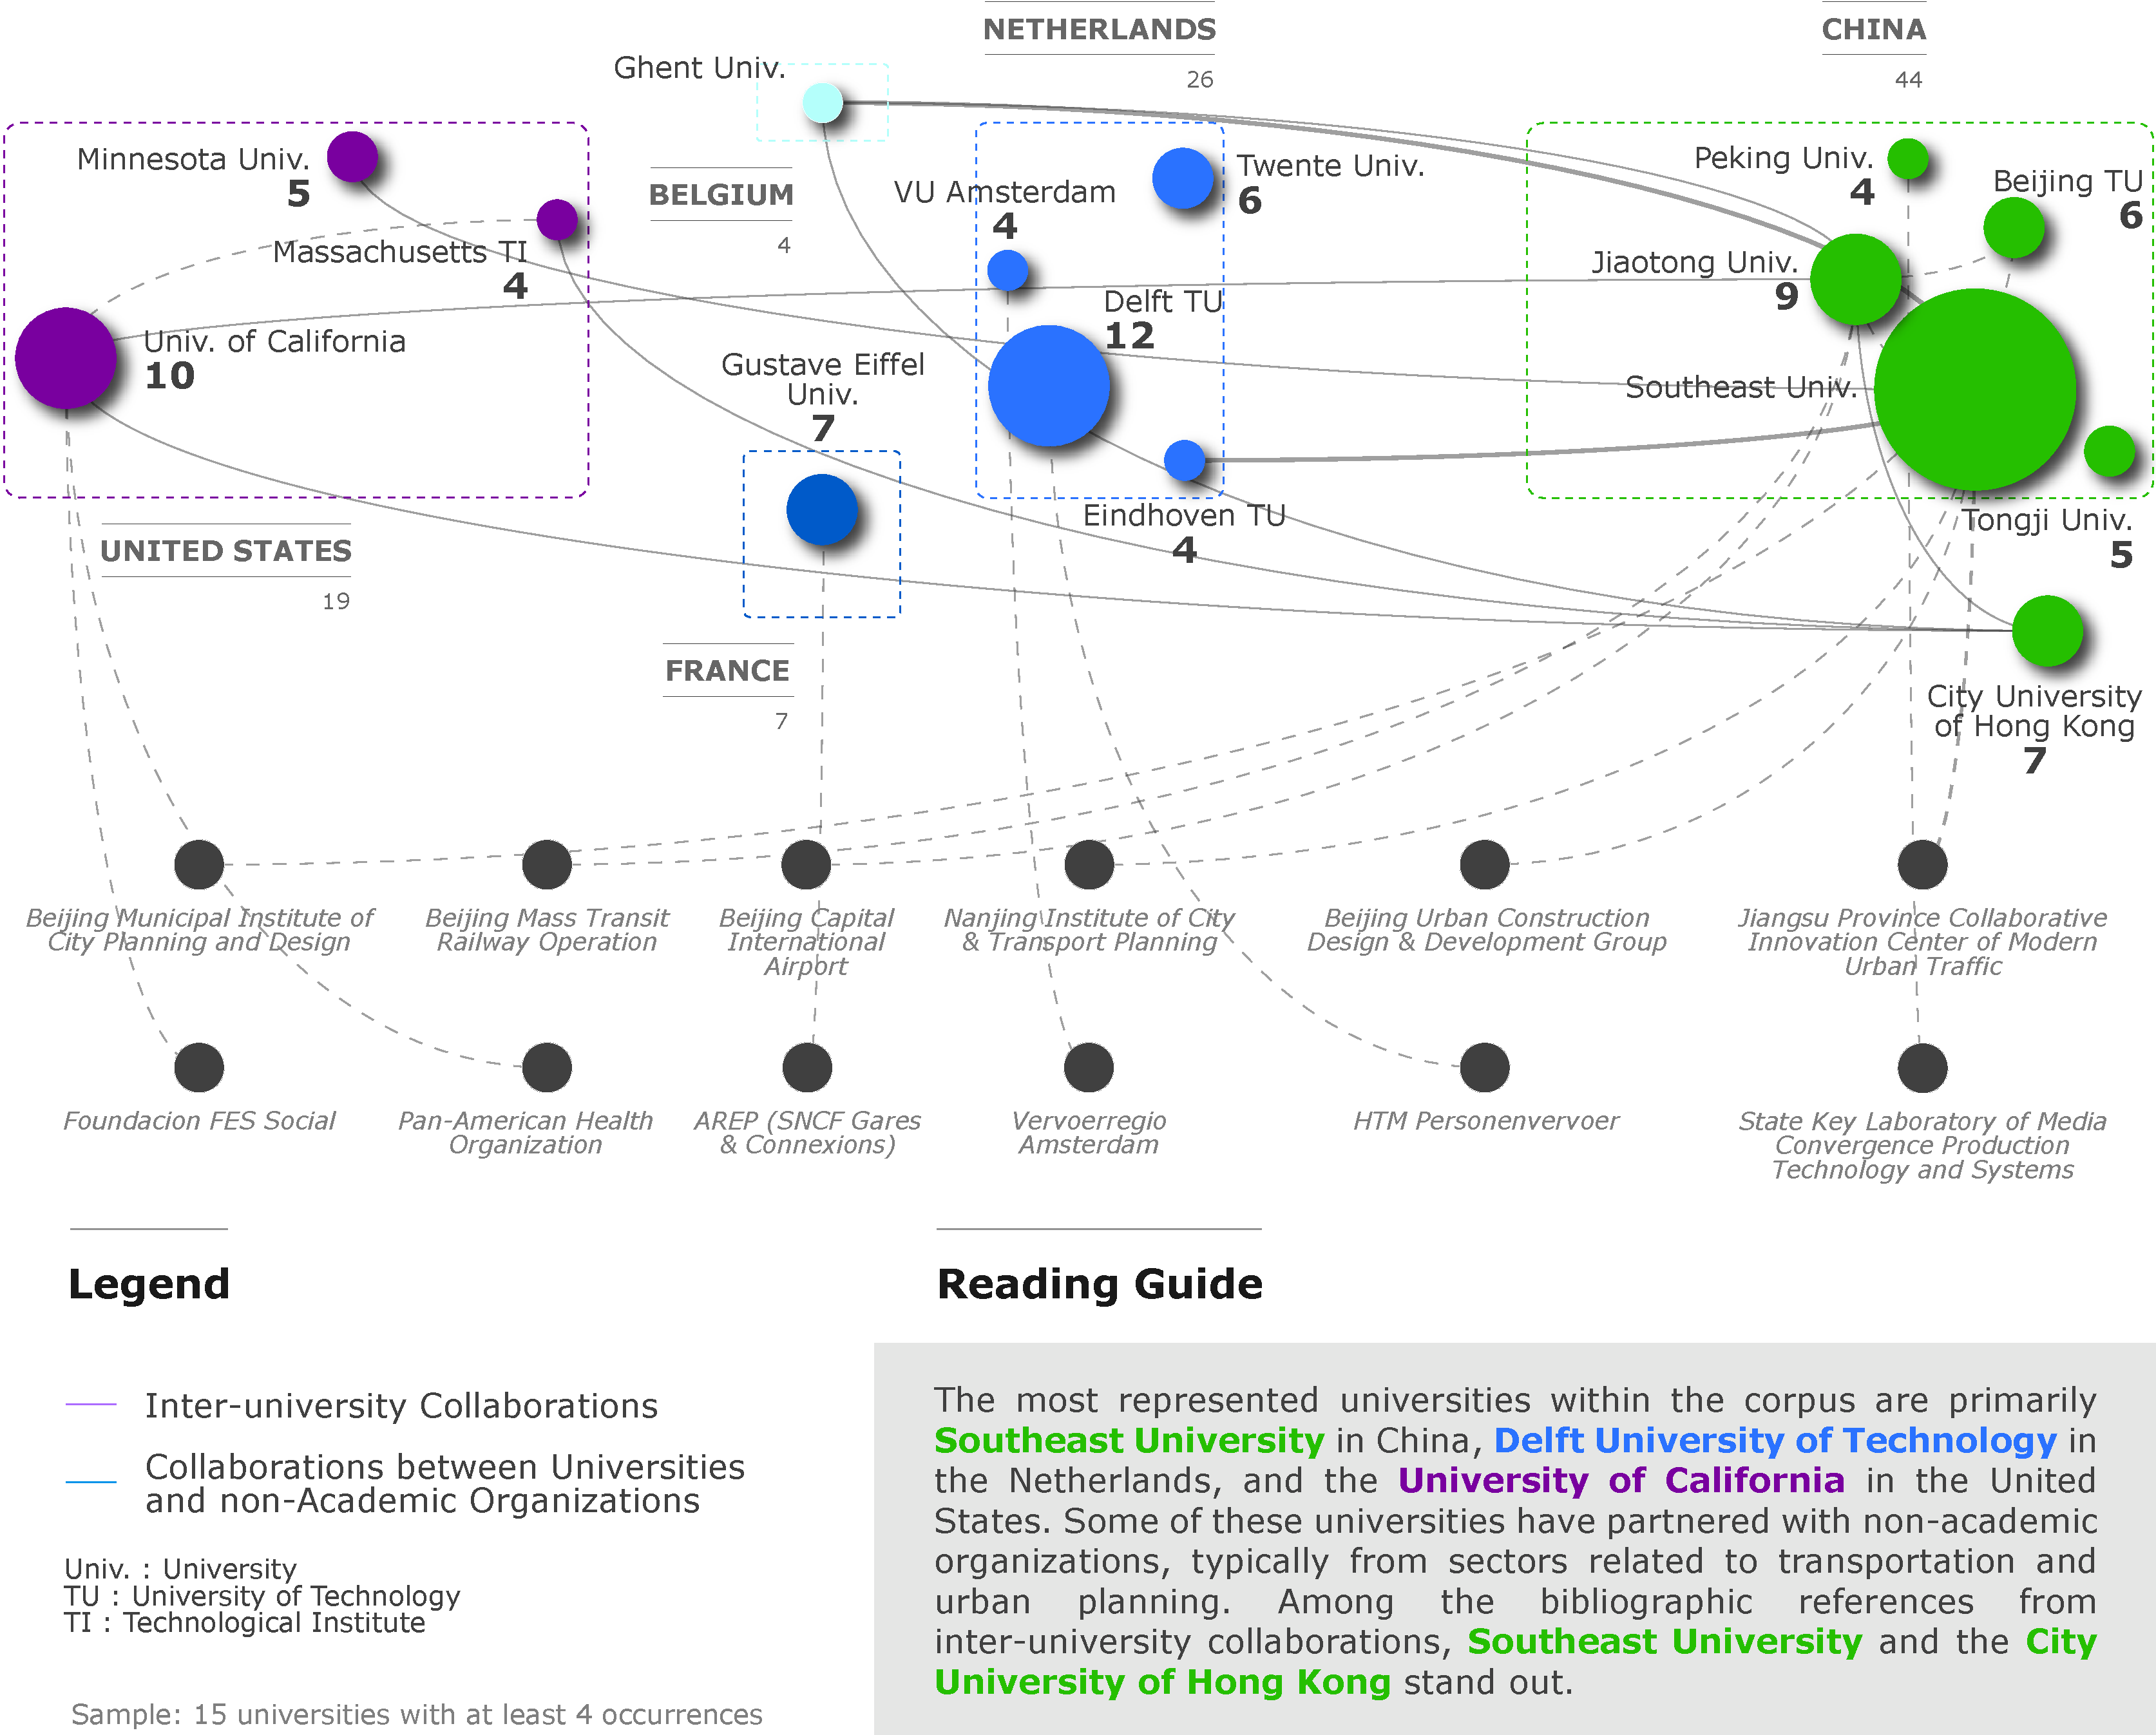
\includegraphics[width=1\columnwidth]{src/Figures/Chap-2/EN_RSL_Collaborations_universites.pdf}}
    \vspace{5pt}
    \begin{flushright}\scriptsize{
    Author: \textcolor{blue}{Dylan Moinse (2023)}
    %\\
    %Created with \Marque{Excel}~and \Marque{Illustrator}
    }\end{flushright}
\end{figure}

    % Universities and Institutions
From the perspective of the institutions represented in the 238 scientific contributions incorporated within the \acrshort{SLR}, a total of 268 unique universities, institutes, organizations, and public or private companies emerge. The fifteen most recurrent institutions represent more than a quarter of the distribution (429 observed values). As shown in \hyperref[fig-chap2:copublications-universites-rsl]{Figure~\ref{fig-chap2:copublications-universites-rsl}} (page~\pageref{fig-chap2:copublications-universites-rsl}), the main universities identified in the documentation are Southeast University in Nanjing (20), followed by Delft University of Technology (12), the University of California, Berkeley (10), Beijing Jiaotong University (9), The Hong Kong Polytechnic University (7), Université Gustave Eiffel in France (7), Beijing University of Technology (6), University of Twente in Enschede (6), Tongji University in Shanghai (5), University of Minnesota Twin Cities in Minneapolis and Saint-Paul (5), Vrije Universiteit Amsterdam (4), Eindhoven University of Technology (4), Ghent University (4), Massachusetts Institute of Technology in Cambridge (4), and finally Peking University (4). %%Translated%%

    % University and Institution Collaborations
By examining scientific collaborations at the university level, it turns out that 128 scientific works are marked by the intersection of at least two academic institutions or research institutes within the same publication. Thus, more than half of the scientific contributions recorded are marked by multi-university co-publications, often spanning distinct continents. The prominent connections observed are concentrated between China, the United States, France, the Netherlands, and Belgium. Among the partnerships that led to such publications, we cite the joint work of Southeast University with Eindhoven University of Technology \textcolor{blue}{\autocite[]{gan_associations_2021, liu_use_2020, liu_understanding_2020}}\index{Gan, Zuoxian|pagebf}\index{Yang, Min|pagebf}\index{Zeng, Qingcheng|pagebf}\index{Timmermans, Harry~J.~P.|pagebf}\index{Liu, Yang|pagebf}\index{Feng, Tao|pagebf}\index{Ji, Yanjie|pagebf}\index{Shi, Zhuangbin|pagebf}\index{Ji, Yanjie|pagebf}\index{Feng, Tao|pagebf}\index{Timmermans, Harry~J.~P.|pagebf} and with Ghent University \textcolor{blue}{\autocite[]{chen_what_2022, cheng_comparison_2023, cheng_exploring_2022}}\index{Chen, Wendong|pagebf}\index{Chen, Xuewu|pagebf}\index{Chen, Jingxu|pagebf}\index{Cheng, Long|pagebf}\index{Huang, Jie|pagebf}\index{Jin, Tanhua|pagebf}\index{Chen, Wendong|pagebf}\index{Li, Aoyong|pagebf}\index{Witlox, Frank|pagebf}\index{Cheng, Long|pagebf}\index{Wang, Kailai|pagebf}\index{Vos, Jonas de|pagebf}\index{Huang, Jie|pagebf}\index{Witlox, Frank|pagebf}, as well as Hong Kong Polytechnic University with the University of California \textcolor{blue}{\autocite{wu_optimal_2020}}\index{Wu, Liyu|pagebf}\index{Gu, Weihua|pagebf}\index{Fan, Wenbo|pagebf}\index{Cassidy, Michael~J.|pagebf} and the Massachusetts Institute of Technology \textcolor{blue}{\autocite{cao_e-scooter_2021}}\index{Cao, Zhejing|pagebf}\index{Zhang, Xiaohu|pagebf}\index{Chua, Kelman|pagebf}\index{Yu, Honghai|pagebf}\index{Zhao, Jinhua|pagebf}. Operational stakeholders are also present in \acrshort{M-TOD} research, primarily in the transport management sector, with joint publications between Jiaotong University and the public transport operator \textsl{Beijing Mass Transit Railway Operation Corporation Limited} \textcolor{blue}{\autocite{wang_interchange_2016}}\index{Wang, Zi-jia|pagebf}\index{Chen, Feng|pagebf}\index{Xu, Tian-kun|pagebf} and \textsl{Beijing Capital International Airport} \textcolor{blue}{\autocite{fan_how_2019}}\index{Fan, Aihua|pagebf}\index{Chen, Xumei|pagebf}\index{Wan, Tao|pagebf}. Similarly, Southeast University forges links with urban actors such as the \textsl{Nanjing Institute of City \& Transport Planning Co.} \textcolor{blue}{\autocite{zhong_layout_2021}}\index{Zhong, Hongming|pagebf}\index{Liu, Zijian|pagebf}\index{Chen, Jun|pagebf}\index{Hao, Jun|pagebf}\index{Wang, Wei|pagebf} and \textsl{Beijing Urban Construction Design \& Development Group Co., Limited} \textcolor{blue}{\autocite{yang_empirical_2016}}\index{Yang, Min|pagebf}\index{Liu, Xinlu|pagebf}\index{Wang, Wei|pagebf}\index{Li, Zhibin|pagebf}\index{Zhao, Jingyao|pagebf}. Furthermore, connections are forming between the University of California and the non-profit organization \acrfull{FES} and the public health organization \textsl{Pan American Health Organization} \textcolor{blue}{\autocite{cervero_influences_2009}}\index{Cervero, Robert|pagebf}\index{Sarmiento, Olga~L.|pagebf}\index{Jacoby, Enrique|pagebf}\index{Gomez, Luis Fernando|pagebf}\index{Neiman, Andrea|pagebf}.%%Translated%%

    % Transition
The bibliometric analysis of the academic corpus focused on a large body of literature, mainly composed of peer-reviewed scientific articles published in English. The analysis framework of the \acrshort{SLR}, based in this first subsection on the contours of research related to \acrshort{M-TOD}, provided an overview of the figures, academic institutions, and scientific journals most influential in this field of study. In the following subsection, we propose to explore the current state of the scientific literature dedicated to \acrshort{TOD} revisited by individual light mobility by conducting a textual analysis of the scientific contributions.%%Translated%%

    % 2.2.1.2. Keywords, Content/Body of the Text
    \needspace{1\baselineskip} % Reserve space
\subsubsection*{Textual Analysis of Academic Publications
    \label{chap2:analyse-textuelle}
    }

    % Introduction
The investigation of the metadata extracted from the academic corpus is, in a second step, based on the lexical systems employed within the research works. This part of the \acrshort{SLR}, intrinsically linked to the textual analysis of academic publications on \acrshort{M-TOD}, aims to identify research practices manifested through the vocabulary used. Initially, the study was differentiated by the language of publication, with the first category being in English, comprising 228 documents, and a second in French, consisting of 10 works. However, due to the low representativity of the French-language works, the textual analysis focuses exclusively on the English-language publications.%%Translated%%

    % Keyword Analysis: Sample and Methodology
Symbolically, the textual examination focused on the content of the research works included in the \acrshort{SLR}, by examining the semantic architecture of the written works, constructed based on the selection of keywords that typically appear after the title and abstract. The aggregation of the academic contributions resulted in the compilation of 1,336 keywords from 208 works, 201 of which are in English. The exploration of the keyword lists defined by the researchers involved in \acrshort{M-TOD} reveals an average of 6.7 keywords per document, considering over 303 distinct terms, of which 260 are in English. To conduct a comparative analysis of the keywords mentioned in the corpus, a preliminary data cleaning phase was undertaken. This process of terminological harmonization involved standardizing keyword sets that share a common origin or related meaning\footnote{~
    For example, the aggregation of the words \Commas{bicyclette}~and \Commas{vélo} in French, or the expressions \Commas{\textsl{transit}}~and \Commas{\textsl{public transport}}, or \Commas{\textsl{subway}}~and \Commas{\textsl{metro}} in English. Although this step is crucial for improving the relevance of the textual data used, it is important to note the assumptions inherent in this work of evaluation.
}.%%Translated%%

    % Keywords: result 1
By cross-referencing the 1,281 English keywords, the textual analysis of this \acrshort{SLR} highlights eleven thematic aspects that stand out within the lexical labels extracted. To conduct this lexical analysis, we first established several thematic categories. Each word was arbitrarily classified according to the category corresponding to its usage context. A graphical highlight of \hyperref[fig-chap2:nuage-mots-cles-rsl]{Figure~\ref{fig-chap2:nuage-mots-cles-rsl}} (page~\pageref{fig-chap2:nuage-mots-cles-rsl}) reveals the clusters of keywords, within which themes related to individual and collective mobility occupy a dominant position. Thus, the concepts related to \Commas{individual modes of transport} (282 occurrences), \Commas{intermodality} (224 occurrences), \Commas{public transport} (202 occurrences), and \Commas{mobility} (181 occurrences) represent the main categories of the ranking, in line with the expression configuration used for the bibliographic search of the \Commas{Corpus EN and FR}, which specifically led to the emergence of these themes (for reference, see \hyperref[table-chap2:expression-recherche-rsl]{Table~\ref{table-chap2:expression-recherche-rsl}}, page~\pageref{table-chap2:expression-recherche-rsl}).%%Translated%%

    % Figure Keyword Cloud RSL
    \begin{figure}[h!]\vspace*{4pt}
        \caption{English keyword clouds extracted from the systematic literature review and classified by theme.}
        \label{fig-chap2:nuage-mots-cles-rsl}
        \centerline{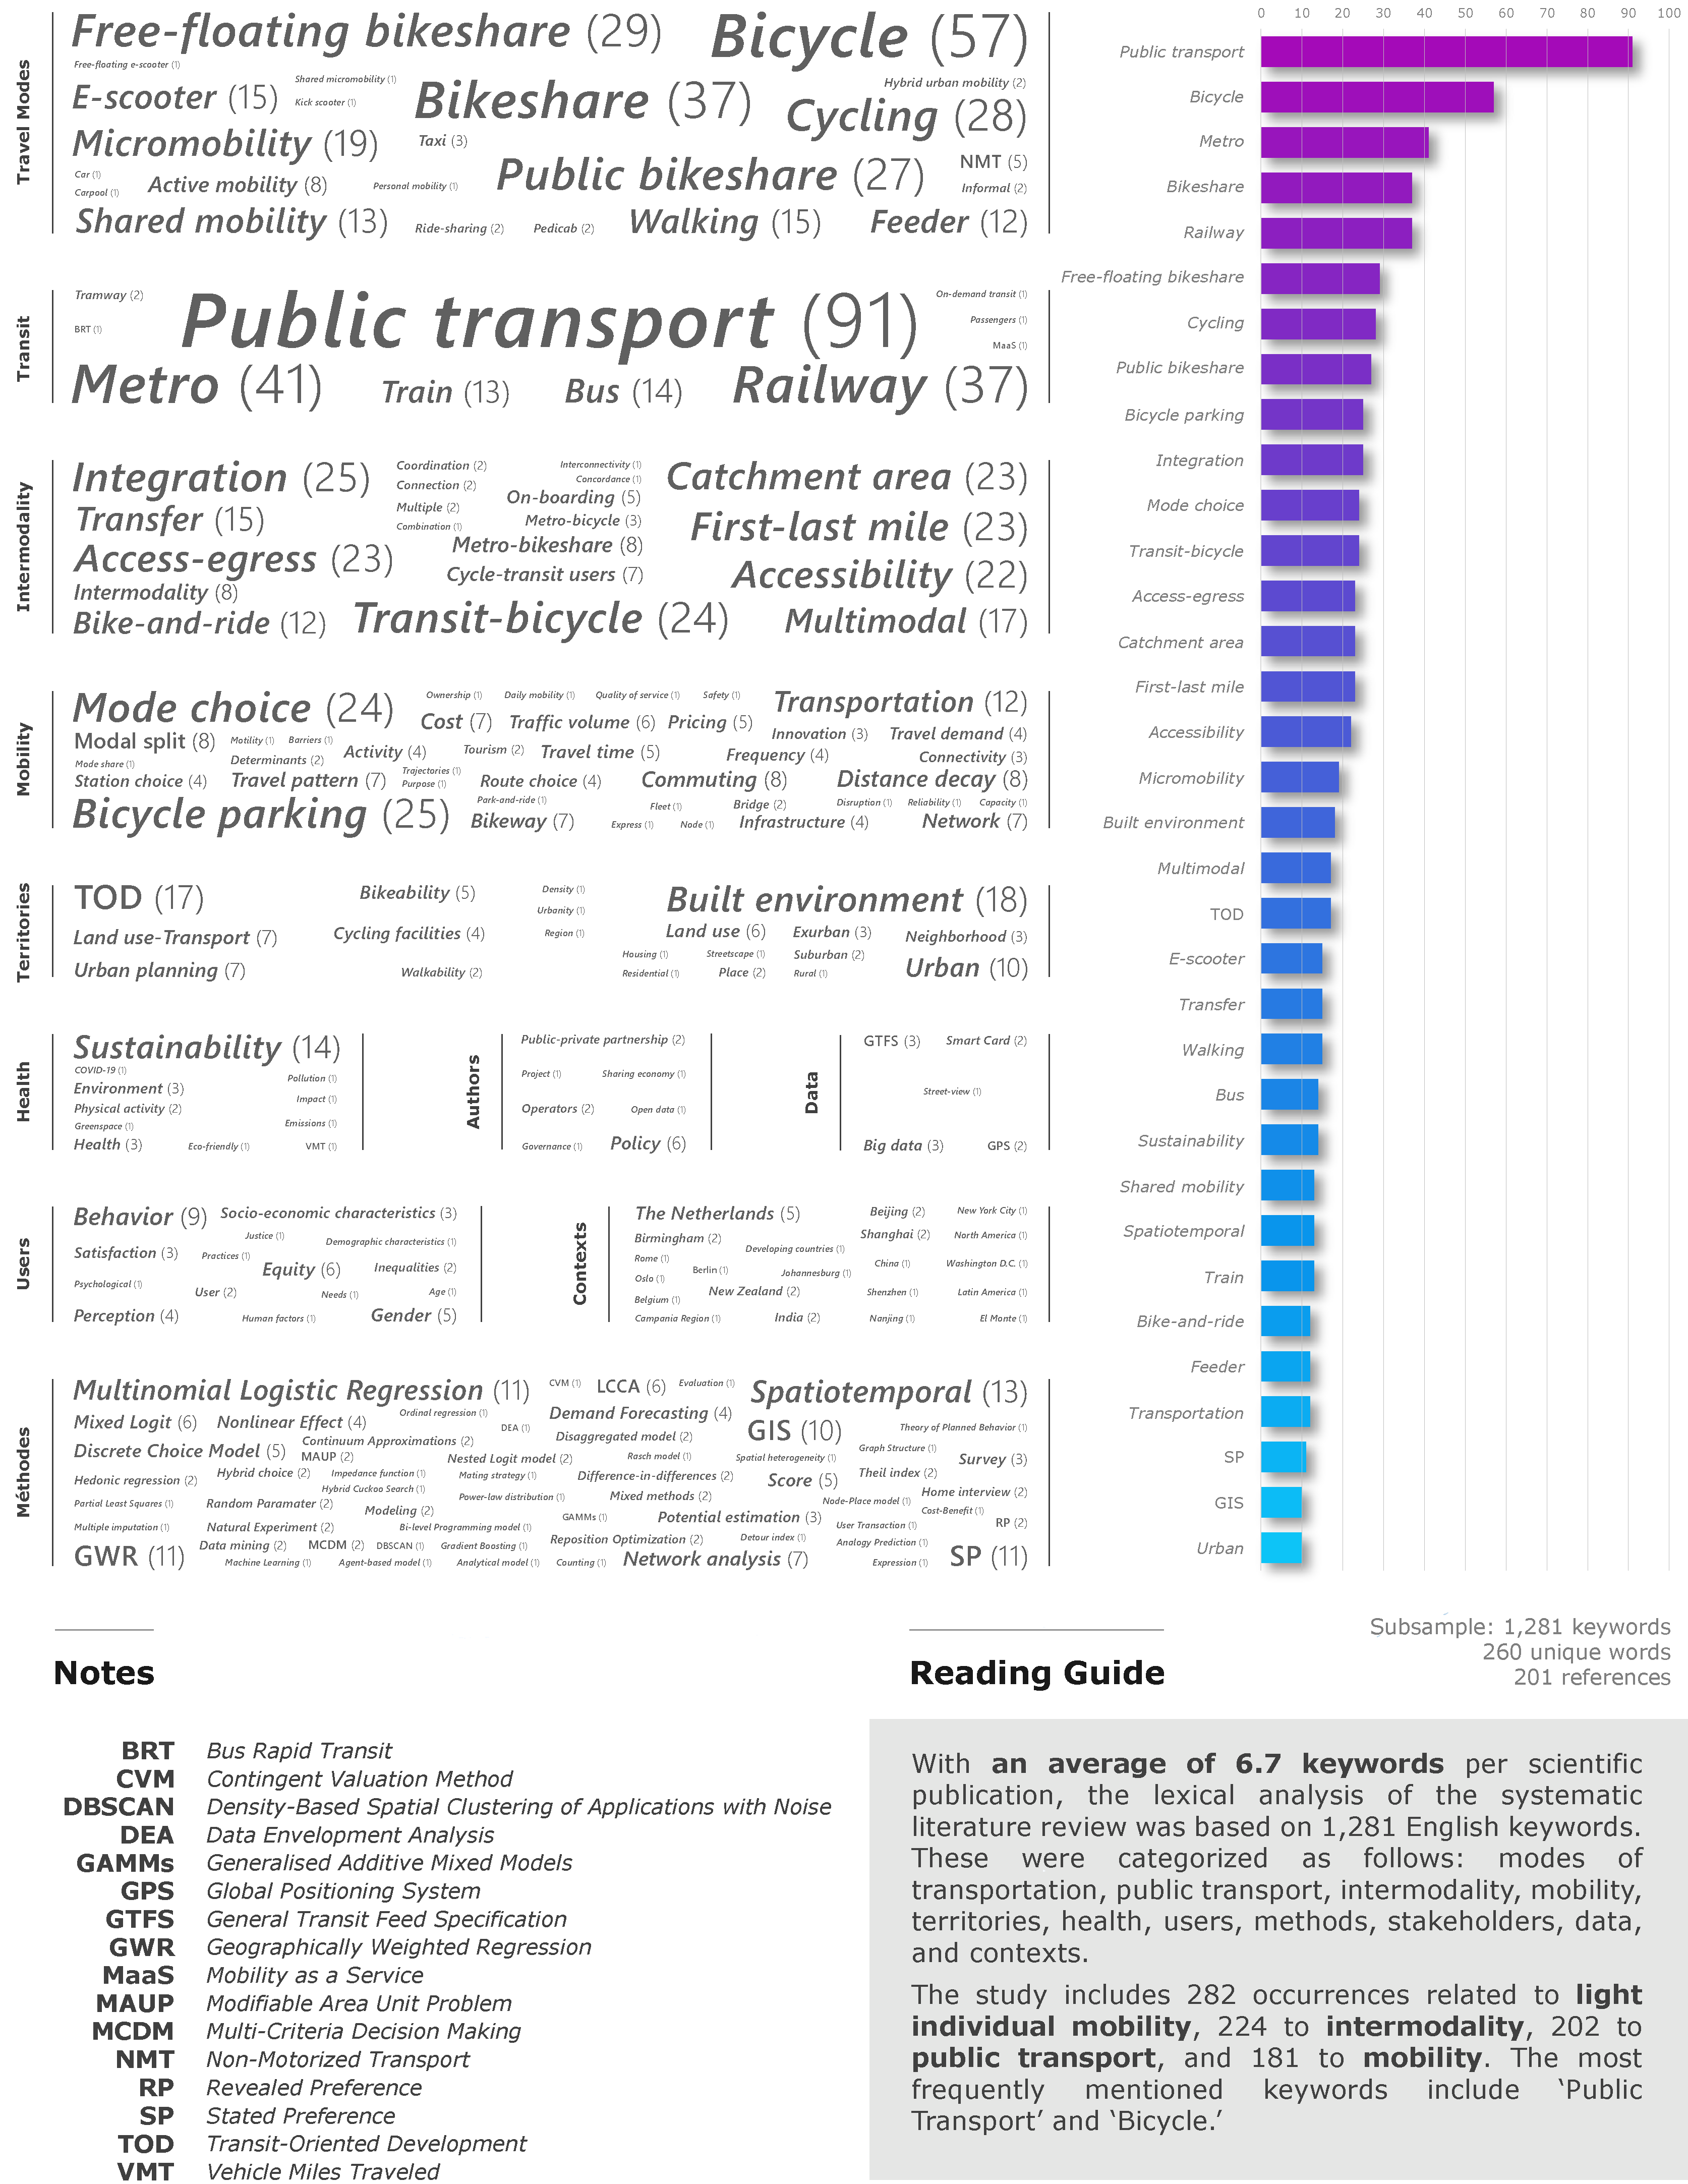
\includegraphics[width=1\columnwidth]{src/Figures/Chap-2/EN_RSL_Nuage_mots_cles_thematiques.pdf}}
        \vspace{5pt}
        \begin{flushright}\scriptsize{
        Author: \textcolor{blue}{Dylan Moinse (2023)}
        %\\
        %Created with \Marque{Python}~and \Marque{Illustrator}
        }\end{flushright}
    \end{figure}

    % Keywords: result 2
At the level of the keywords, it is primarily in the fields of \Commas{public transport} and \Commas{bicycle} that prominent occurrences are found, counting respectively 91 and 57 iterations of terms associated with them. However, this predominance of keywords masks an unequal distribution within each observed theme. While the frequency of keywords related to \Commas{public transport}, \Commas{individual modes of transport}, and \Commas{intermodality} is significant, averaging 20, 12, and 11 occurrences per term, this intensity diminishes to 5.5 and 2 repetitions regarding the categories related to \Commas{mobility}, \Commas{urban planning}, and \Commas{methods}. This observation reflects a broader variety of keywords in these latter themes, alongside a process of terminological homogenization noticeable within the domains of personal transport modes, public transport, and intermodality.%%Translated%%

    % Keywords: result 3
The manipulation of keywords from the perspective of transport modes and infrastructures as objects, such as \Commas{\textsl{bicycle}} (mentioned 57 times), \Commas{\textsl{dockless bikeshare}} (29 occurrences), \Commas{\textsl{public bikeshare}} (27 occurrences), \Commas{\textsl{metro}} (41 occurrences), \Commas{\textsl{railway}} (37 occurrences), and \Commas{\textsl{bicycle parking}} (25 occurrences), reflects an interconnection that crystallizes into lexical signals, perpetuating the conventional pattern in the transport domain (see \hyperref[fig-chap2:nuage-mots-cles-rsl]{Figure~\ref{fig-chap2:nuage-mots-cles-rsl}}, page~\pageref{fig-chap2:nuage-mots-cles-rsl}). Analogous to this approach grounded in the transport paradigm, a vast semantic domain related to the \Commas{turning point of mobility} \textcolor{blue}{\autocites{sheller_new_2006}[8]{sheller_mobilizing_2016}[13]{randell_no_2020}}\index{Sheller, Mimi|pagebf}\index{Urry, John|pagebf}\index{Randell, Richard|pagebf}, is marked by the use of expressions such as \Commas{\textsl{accessibility}} (22 occurrences), \Commas{\textsl{sustainability}} (14 occurrences), \Commas{\textsl{behavior}} (9 occurrences), \Commas{\textsl{policy}} (6 occurrences), \Commas{\textsl{equity}} (6 occurrences), and \Commas{\textsl{bikeability}} (5 occurrences). Indeed, to a lesser extent, we can discern the involvement of urban planning and particularly its connection with mobility, as evidenced by the concept of \Commas{\textsl{TOD}} (17 occurrences) or \Commas{\textsl{land use-transport}} (7 occurrences).%%Translated%%

    % Keywords: result 4
By probing the interactions between the aforementioned keywords, it is interesting to note the close links that associate certain categories with each other. The majority of the word lists tend to establish connections between the categories of \Commas{public transport} and \Commas{individual modes of transport}. Among the 201 English references, 155 of them create a dialogue between these two themes, expressed by the deliberate choice of a list of keywords related to collective and personal mobility. Furthermore, 59 scientific publications stand out for their specific configuration, forming an ordered lexical sequence as follows: the first keyword in the list refers to \Commas{public transport}, followed by \Commas{individual modes of transport}, and a third term invoking \Commas{intermodality}.%%Translated%%

    % Figure Keywords content RSL
    \begin{figure}[h!]\vspace*{4pt}
        \caption{Keyword cloud from the full content of the English-language academic works included in the systematic literature review.}
        \label{fig-chap2:contenu-textuel-rsl}
        \centerline{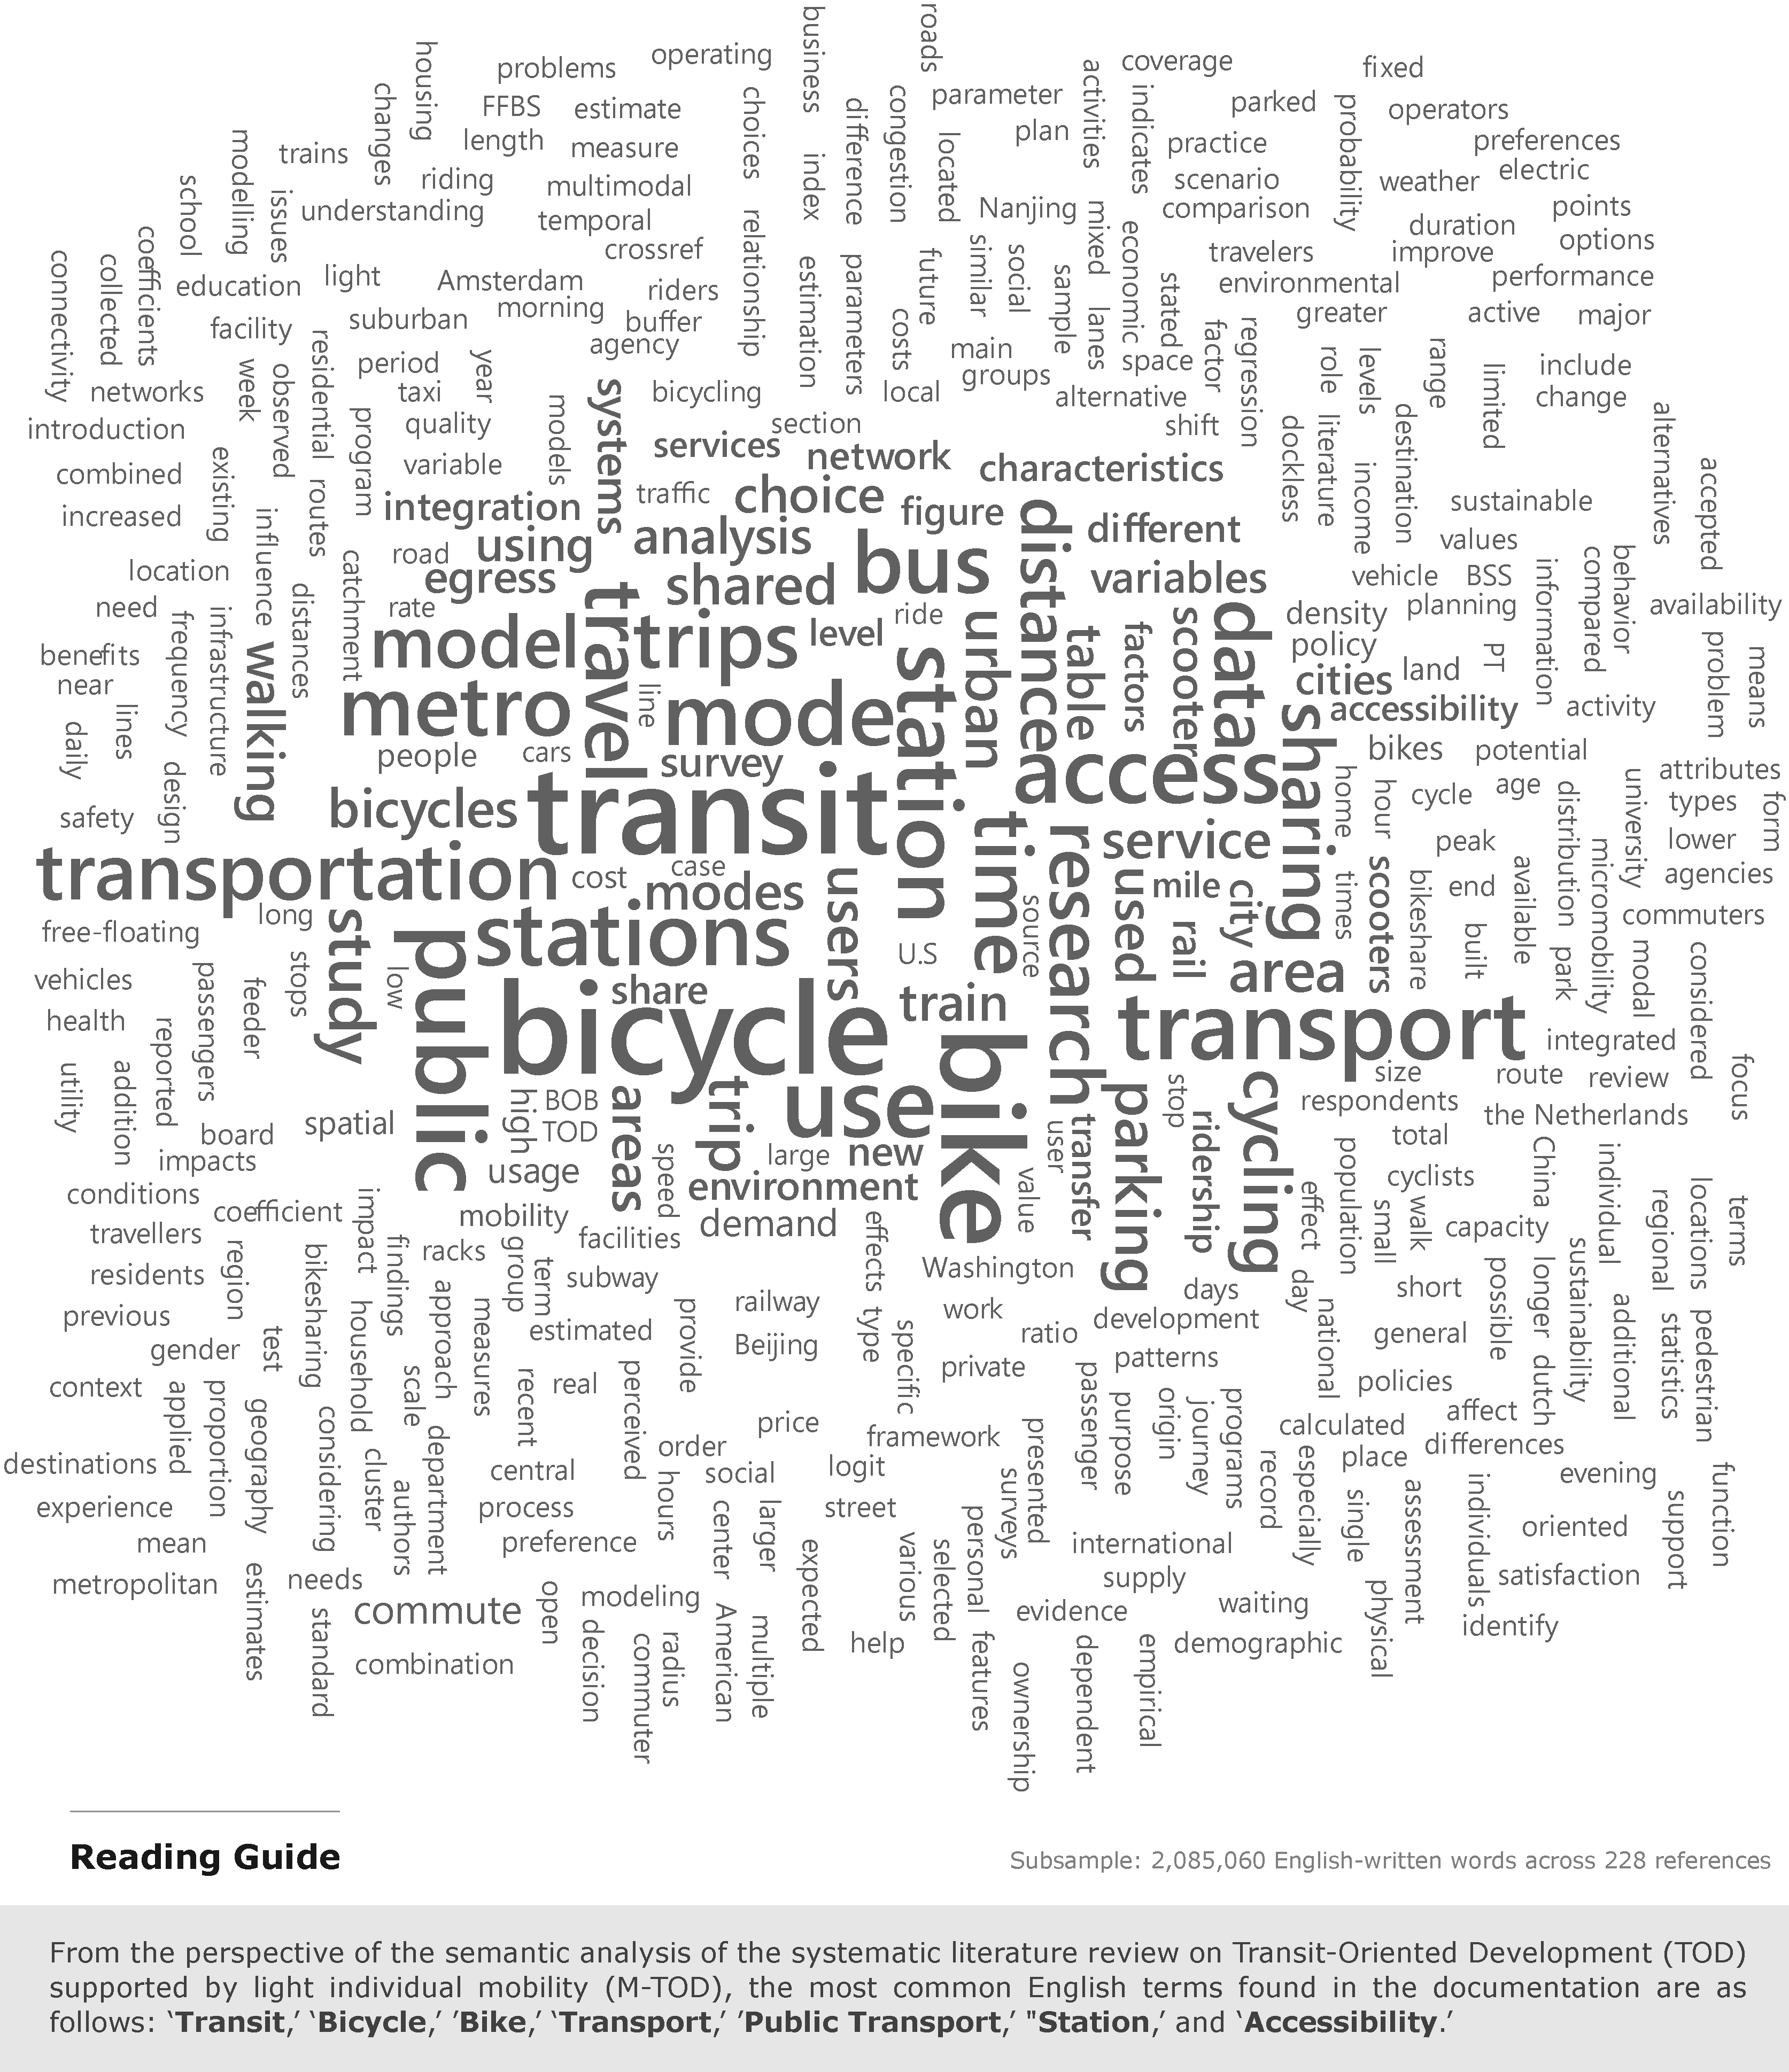
\includegraphics[width=1\columnwidth]{src/Figures/Chap-2/EN_RSL_Mots_contenu.pdf}}
        \vspace{5pt}
        \begin{flushright}\scriptsize{
        Author: \textcolor{blue}{Dylan Moinse (2023)}
        %\\
        %Created with \Marque{Python}~and \Marque{Illustrator}
        }\end{flushright}
    \end{figure}

    % RSL Word Content
The textual analysis was deepened through an examination of the full content of each English-language scientific publication. As shown in \hyperref[fig-chap2:contenu-textuel-rsl]{Figure~\ref{fig-chap2:contenu-textuel-rsl}} (page~\pageref{fig-chap2:contenu-textuel-rsl}), the examination of the hundred most recurrent terms within the documents\footnote{~
    In order to classify the lexical fields identified in the analyzed documents, we first performed a cleaning step by excluding terms related to everyday life or general scientific research in the English language. These common expressions were later excluded from the analysis, such as \Commas{\textsl{the}}, \Commas{\textsl{a}}, \Commas{\textsl{and}}, \Commas{\textsl{we}}, \Commas{\textsl{for}}, \Commas{\textsl{study}}, \Commas{\textsl{scientific}}, \Commas{\textsl{methods}} and \Commas{\textsl{results}}.
} reinforces the trend previously identified at the keyword level, primarily marked by the predominance of terms such as \Commas{\textsl{transit}}, \Commas{\textsl{bicycle}}, \Commas{\textsl{bike}}, \Commas{\textsl{transport}}, \Commas{\textsl{public transport}}, \Commas{\textsl{station}}, and \Commas{\textsl{accessibility}}. However, it is important to highlight the substantial influence of some terms, such as \Commas{\textsl{use}}, \Commas{\textsl{access}}, \Commas{\textsl{distance}}, \Commas{\textsl{area}}, \Commas{\textsl{users}}, or \Commas{\textsl{service}}, which are related to usage, users, and distances or travel times. On the other hand, it should be noted that the lexical presence related to urban planning remains practically absent in the writings, except for a few event-driven occurrences, such as \Commas{\textsl{density}}, \Commas{\textsl{mixed}}, \Commas{\textsl{TOD}}, or \Commas{\textsl{land}}.%%Translated%%

    % Transition
Upon reviewing the terms scrutinized within the \acrshort{SLR} corpus, the various collective and individual transport modes, central to a transit-oriented urban development supported by individual light mobility, emerge as the foremost themes. Given the rapid evolution of mobility practices, technologies, and techniques pertaining to these different transportation modes, the following subsection aims to contextualize research works related to the \acrshort{M-TOD}, focusing on the development of emerging areas of investigation.%%Translated%%

    % 2.2.1.3. micromobility, TC
    \needspace{1\baselineskip} % Space reservation
\subsubsection*{Evolution of Research on the Synergy between Public Transport and Light Individual Mobility
    \label{chap2:evolution-recherches-tc-mobilite-individuelle-legere}
    }

    % Trend Since 1993
The analysis of the temporal distribution of the scientific publications included in the \acrshort{SLR} offers a comprehensive perspective on the characteristics and advancements that delimit this body of literature. The chronological trajectory of the bibliographic corpus dedicated to the integration of light individual mobility into public transport networks depicts continuous growth between 1993 and 2021. From 2015 onward, the annual threshold of ten scientific publications was consistently exceeded, suggesting growing research interest in this topic. In just four consecutive years, the number of academic papers doubled, with 129 new works published between 2019 and the beginning of 2023.%%Translated%%

    % Objective
In line with the methodological protocol defined in this \acrshort{SLR}, the minimum date for this bibliometric study was set to 1993, referencing the conceptualization of \acrshort{TOD} by \textcolor{blue}{Peter} \textcolor{blue}{\textcite{calthorpe_next_1993}}\index{Calthorpe, Peter|pagebf}. The bibliographic study presented here aims to reveal the characteristics of this corpus developed over three decades of international research. However, it is essential to acknowledge the existence of earlier works addressing the subject of study. While the observed growth of scientific publications includes works in both English and French, the emergence of French-language works occurred at a later stage, starting in 2015. However, this subset remains small, making it difficult to draw definitive conclusions. On the other hand, the scientific literature in European contexts began to develop early, as early as 2000.%%Translated%%

    % Figure Chronology RSL Transport Modes
    \begin{figure}[h!]\vspace*{4pt}
        \caption{Evolution of scientific publications on the combination of public transport and light individual mobility within the systematic literature review.}
        \label{fig-chap2:chronologie-modes-deplacements-rsl}
        \centerline{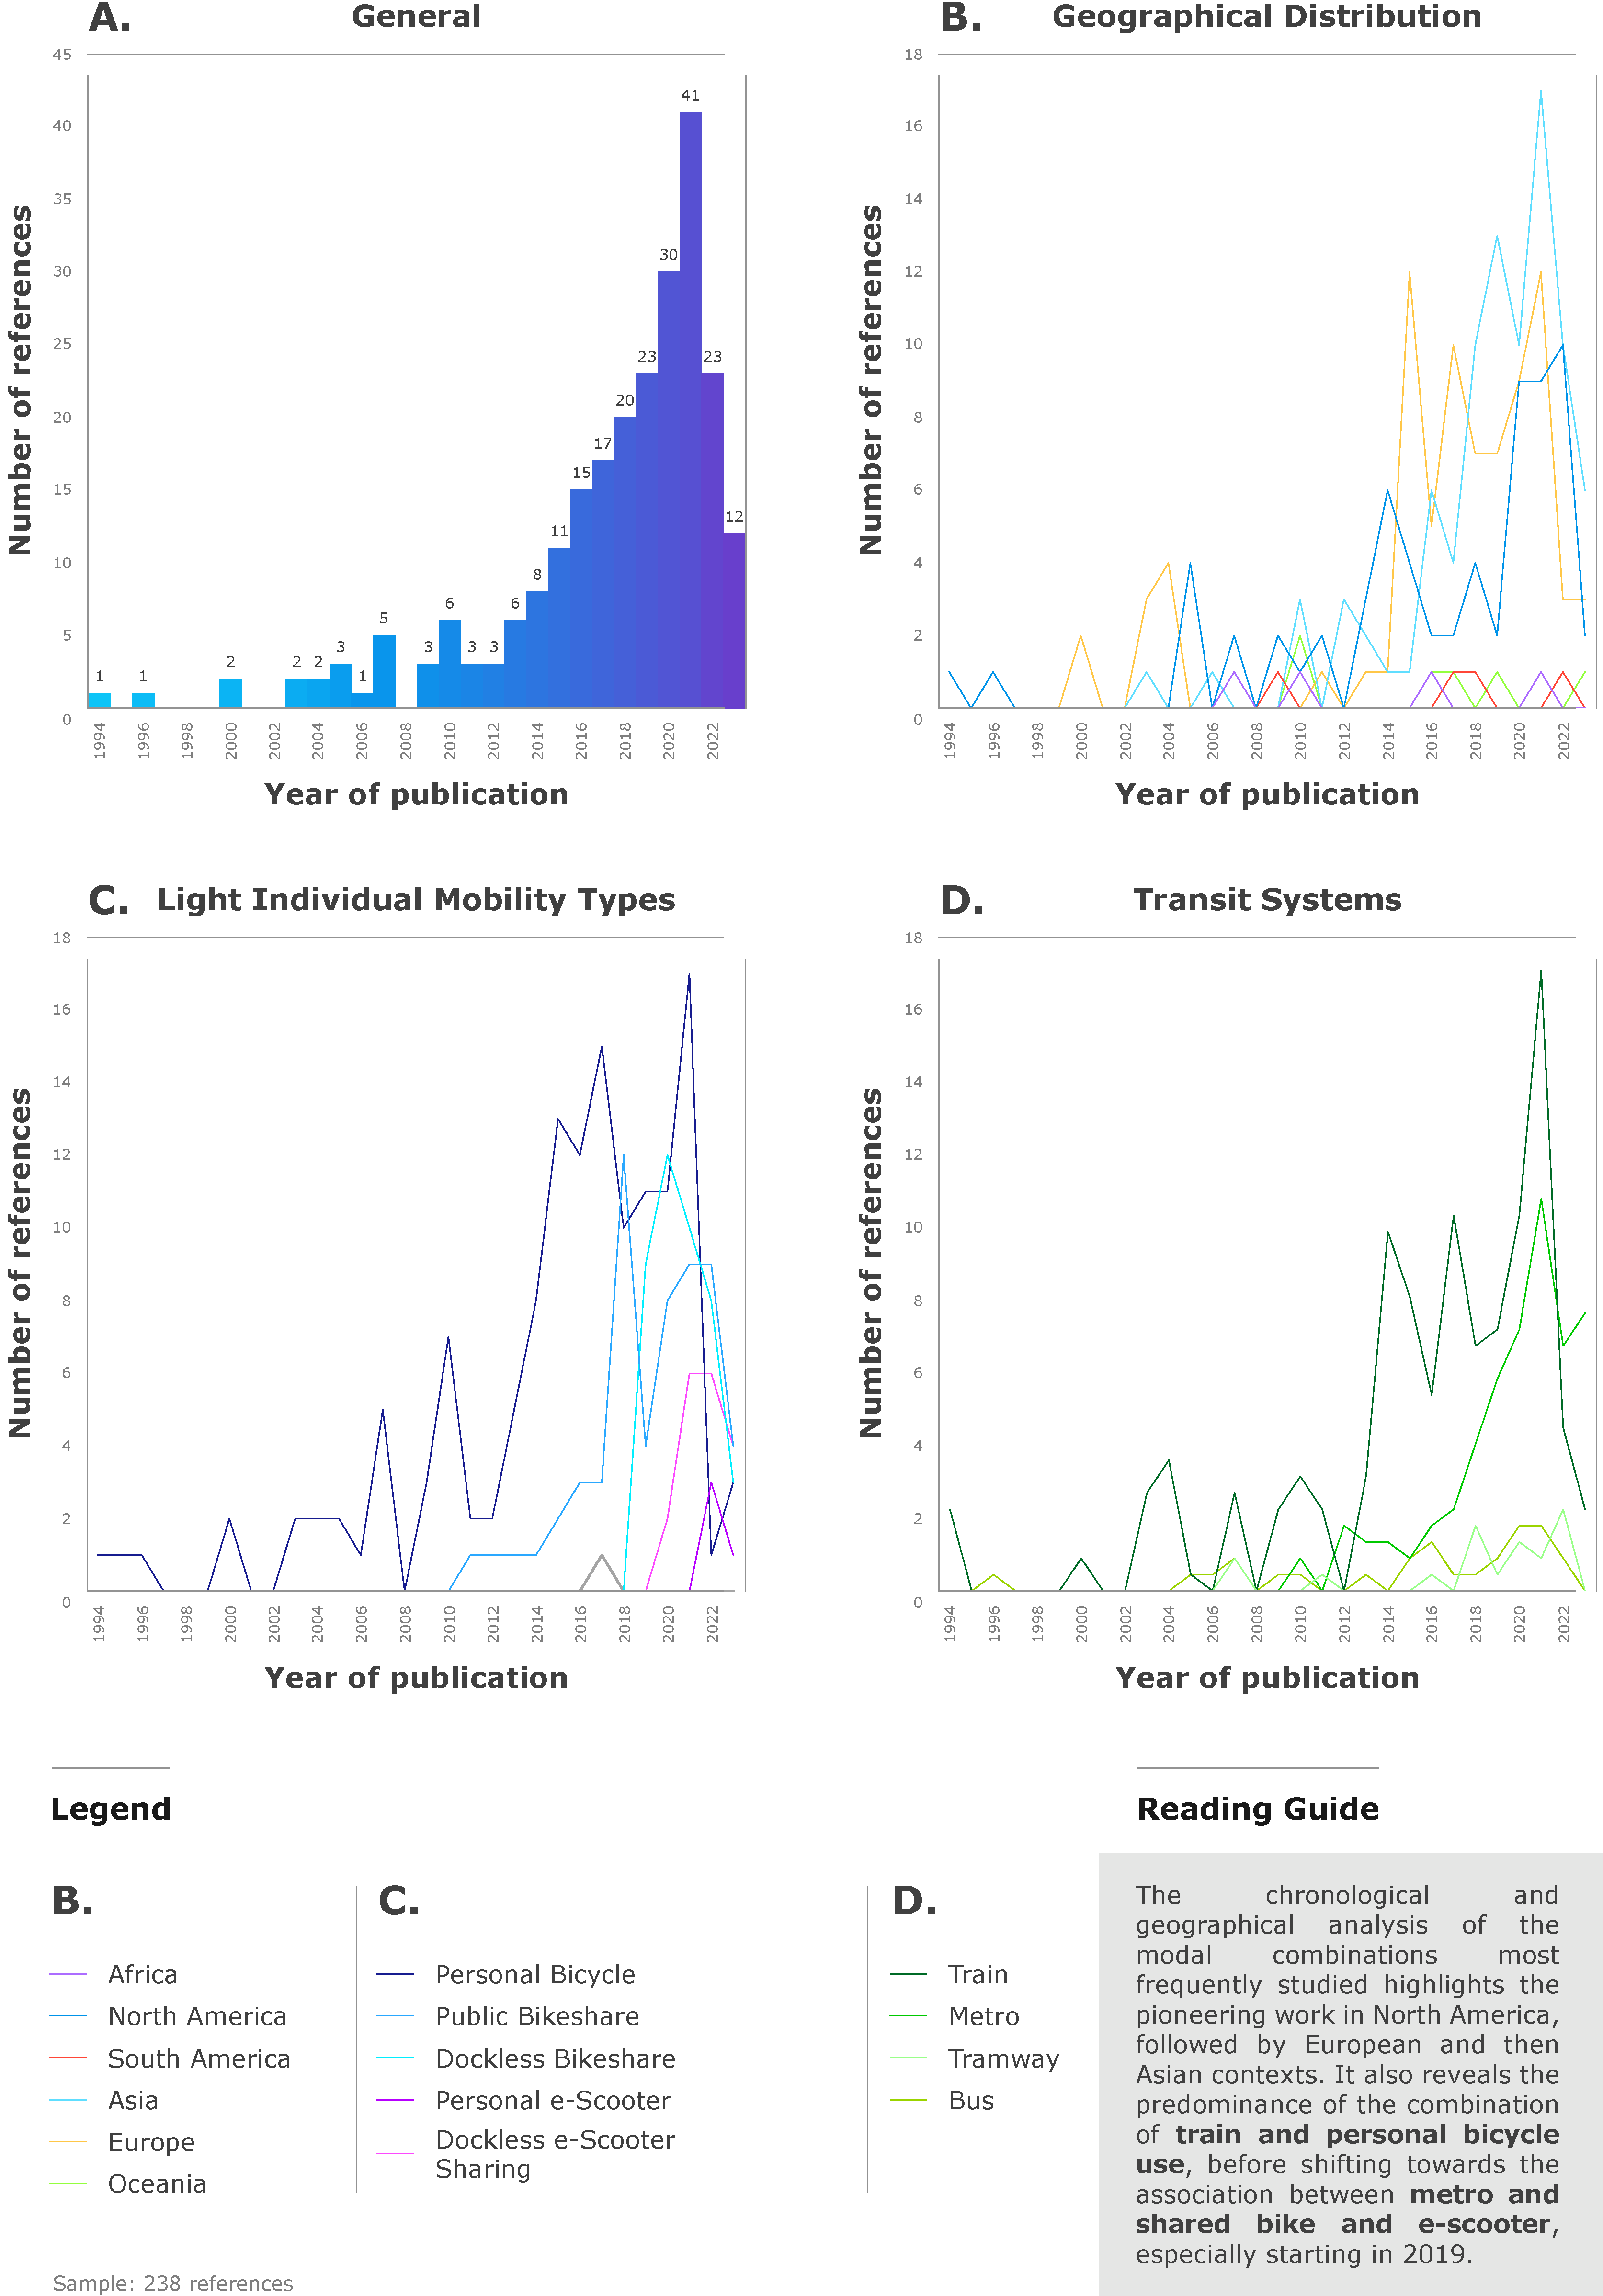
\includegraphics[width=1\columnwidth]{src/Figures/Chap-2/EN_RSL_Chronologie.pdf}}
        \vspace{5pt}
        \begin{flushright}\scriptsize{
        Author: \textcolor{blue}{Dylan Moinse (2023)}
        %\\
        %Created with \Marque{Excel}, \Marque{Python}, and \Marque{Illustrator}
        }\end{flushright}
    \end{figure}

    % Chronology by Micromobility
The chronological approach to \acrshort{M-TOD}, as depicted in the scientific literature, offers insightful perspectives on the rise of light individual mobility (see \hyperref[annexes:rsl-combinaisons-modales]{Appendix~\ref{annexes:rsl-combinaisons-modales}}, page~\pageref{annexes:rsl-combinaisons-modales}) and its potential contribution to the development of the urban model. \hyperref[fig-chap2:chronologie-modes-deplacements-rsl]{Figure~\ref{fig-chap2:chronologie-modes-deplacements-rsl}} (page~\pageref{fig-chap2:chronologie-modes-deplacements-rsl}) reveals the prominent role that conventional bicycles held in international research from 1994 to 2017, representing 89\% of the publications during that period. However, this dominant position has gradually been challenged, with the traditional bicycle being present in only 41\% of studies between 2018 and 2021, and in just 4\% of the most recent publications. This unfavorable trend initially benefited the exploration of \acrfull{PBS}, which saw increased interest starting in 2011. Later, from 2019 onwards, attention shifted to \acrfull{DBS}. More recently, the research corpus has shown a growing interest in \acrfull{DESS}. However, \acrfull{PeS} remains absent from the studies, highlighting a stark contrast between the recent boom in research on shared mobility services and the scarcity of studies on private electric scooter use. This observation should be understood within the context of the rise of shared bicycles and micromobility, as evidenced by the descriptive analysis conducted by \textcolor{blue}{\textcite[298]{zhang_built_2023}}\index{Zhang, Yushan|pagebf}\index{Kasraian, Dena|pagebf}\index{Wesemael, Pieter van|pagebf} in their \acrshort{SLR}, which shows that three-quarters of the documentation on this subject emerged between 2019 and 2022.%%Translated%%

    % Chronology by Public Transport
The sequential study of public transport systems examined in the scientific literature also sheds light on the general trends that have emerged over the three decades under investigation. As indicated in \hyperref[fig-chap2:chronologie-modes-deplacements-rsl]{Figure~\ref{fig-chap2:chronologie-modes-deplacements-rsl}} (page~\pageref{fig-chap2:chronologie-modes-deplacements-rsl}), international research on \acrshort{M-TOD} showed particular interest in intercity rail modes from 1994 to 2017, with particular focus on \acrfull{TER}, in conjunction with the conventional bicycle. In contrast, the metro system, which had been relatively overlooked until 2012, saw a resurgence of interest from 2019, coinciding with the increased focus on \acrshort{DBS} and \acrshort{DESS} systems. Furthermore, studies on the integration of light individual mobility with buses, particularly \acrfull{BRT}, as well as with trams, maintain a secondary but consistent presence in the scientific publications. Overall, the chronological analysis of the most frequently studied modal combinations reveals a main pattern: the initial dominance of the train and personal bicycle pairing in academic works on \acrshort{M-TOD}, gradually giving way to the combination of metro and bike and micromobility services.%%Translated%%

    % Chronology by Shared Micromobilities (Maturation)
Although the scientific literature on light individual mobility, particularly on shared bicycles and micromobility, has developed in recent years, research focuses on various stages of development of these mobility services in the surveyed territories. By examining the period difference between when the light individual mobility service was launched and when the data was collected and processed in the analyzed documentation, we explored the different maturation stages studied based on the modes of transport involved in bike and scooter sharing. These mobility services are mostly studied during their recent development, about three years (forty months) after being launched in the territory \textcolor{blue}{\autocite[298]{zhang_built_2023}}\index{Zhang, Yushan|pagebf}\index{Kasraian, Dena|pagebf}\index{Wesemael, Pieter van|pagebf}. However, the standard deviation of the observed distribution is quite large, with an average difference of four years, meaning that a significant proportion of research focuses on a more advanced stage of development. This unequal distribution is notably explained by the differences in the type of shared light individual mobility analyzed:
    \begin{customitemize}
        \item The corpus on \acrshort{PBS} systems is the most diverse, with studies mostly focusing on services that have been operational for five years. Notable works by \textcolor{blue}{\textcite{aljeri_impacts_2020, andersson_neighbourhood_2021, ma_estimating_2019, ashraf_impacts_2021, liu_understanding_2020, kuijk_preferences_2022, gu_measuring_2019, kong_deciphering_2020, radzimski_exploring_2021, romm_differences_2022, tarpin-pitre_typology_2020}}\index{Aljeri, Moathe|pagebf}\index{Andersson, David Emanuel|pagebf}\index{Ma, Ting|pagebf}\index{Ashraf, Md Tanvir|pagebf}\index{Liu, Yang|pagebf}\index{Kuijk, Roy~J. van|pagebf}\index{Gu, Tianqi|pagebf}\index{Kong, Hui|pagebf}\index{Radzimski, Adam|pagebf}\index{Dzięcielski, Michał|pagebf}\index{Romm, Daniel|pagebf}\index{Verma, Priyanka|pagebf}\index{Karpinski, Elizabeth|pagebf}\index{Sanders, Tracy~L.|pagebf}\index{McKenzie, Grant|pagebf}\index{Tarpin-Pitre, Léandre|pagebf} focus on the impacts of \acrshort{PBS} on public transport networks in New York City, Taipei, Washington D.C., Nanjing, Suzhou, Boston, and Montreal, between five and seven years after launch. In contrast, \textcolor{blue}{\textcite{cheng_promoting_2022, cheng_expanding_2018, yen_how_2023, tang_uncovering_2021, bocker_bike_2020}}\index{Cheng, Long|pagebf}\index{Jin, Tanhua|pagebf}\index{Wang, Kailai|pagebf}\index{Lee, Yongsung|pagebf}\index{Witlox, Frank|pagebf}\index{Cheng, Yung-Hsiang|pagebf}\index{Yen,~B.T.H.|pagebf}\index{Mulley, Corinne|pagebf}\index{Yeh, Chia-Jung|pagebf}\index{Tang, Jinjun|pagebf}\index{Böcker, Lars|pagebf} analyze the impact of urban environment on mobility systems in Nanjing, Kaohsiung, Taipei, Shenzhen, and Oslo, eight to fifteen years after launch;
        \item \acrshort{DBS} is generally studied two years after its deployment in the territory, while the first quarter of publications on this topic explores the service less than a year after launch. Thus, \textcolor{blue}{\textcite{chen_what_2022, fan_dockless_2020, qiu_interplay_2021, fan_how_2019, jin_competition_2019, li_integration_2020, li_unbalanced_2022, li_factors_2020, liu_use_2020, wu_identification_2023, yang_spatiotemporal_2019}}\index{Chen, Wendong|pagebf}\index{Fan, Yichun|pagebf}\index{Qiu, Waishan|pagebf}\index{Jin, Haitao|pagebf}\index{Jin, Fengjun|pagebf}\index{Wang, Jiao'e|pagebf}\index{Sun, Wei|pagebf}\index{Dong, Libo|pagebf}\index{Li, Jie|pagebf}\index{Li, Lili|pagebf}\index{Li, Xuefeng|pagebf}\index{Liu, Yang|pagebf}\index{Wu, Hao|pagebf}\index{Wang, Yanhui|pagebf}\index{Sun, Yuqing|pagebf}\index{Yin, Duoduo|pagebf}\index{Li, Zhanxing|pagebf}\index{Luo, Xiaoyue|pagebf}\index{Yang, Yuanxuan|pagebf} study the use of \acrshort{DBS} in combination with public transport networks in Nanjing, Beijing, Ithaca, Suzhou, Shenzhen, Nanjing, and Nanchang, one to two years after its introduction. Similarly, as with \acrshort{PBS}, \textcolor{blue}{\textcite{cheng_exploring_2022, chu_last_2021, guo_built_2020, guo_role_2021, hu_study_2019}}\index{Cheng, Long|pagebf}\index{Wang, Kailai|pagebf}\index{Vos, Jonas de|pagebf}\index{Huang, Jie|pagebf}\index{Witlox, Frank|pagebf}\index{Chu, Junhong|pagebf}\index{Duan, Yige|pagebf}\index{Yang, Xianling|pagebf}\index{Wang, Li|pagebf}\index{Guo, Yuanyuan|pagebf}\index{Hu, Li|pagebf}\index{He, Sylvia~Y.|pagebf} focus on the role of the urban environment related to \acrshort{DBS} in intermodality, in Nanjing, Beijing, and Shenzhen;
        \item Lastly, half of the literature on \acrshort{DESS} in combination with public transport adopts a territory benefiting from shared micromobility for less than a year. All the scientific productions on this subject examine the use of \acrshort{DESS} in intermodality, in Seoul, Austin, Rome, Seattle, Oslo, Berlin, New York City, Columbus, Chicago, and Nashville \textcolor{blue}{\autocite{baek_electric_2021, zuniga-garcia_evaluation_2022, vinagre_diaz_blind_2023, beale_integrating_2023, fearnley_patterns_2020, heumann_spatiotemporal_2021, lee_forecasting_2021, li_measuring_2022, mohammadian_analyzing_2022, ziedan_complement_2021}}\index{Baek, Kwangho|pagebf}\index{Zuniga-Garcia, Natalia|pagebf}\index{Vinagre Díaz, Juan José|pagebf}\index{Beale, Kirsten|pagebf}\index{Fearnley, Nils|pagebf}\index{Heumann, Maximilian|pagebf}\index{Li, Mina|pagebf}\index{Li, Xia|pagebf}\index{Mohammadian, Abolfazl|pagebf}\index{Ziedan, Abubakr|pagebf}\index{Shah, Nitesh~R.|pagebf}\index{Wen, Yi|pagebf}\index{Brakewood, Candace|pagebf}\index{Cherry, Christopher~R.|pagebf}\index{Cole, Justin|pagebf}.
    \end{customitemize}%%Translated%%

    % Discussion of Maturation
From this observation, it is clear that bike-sharing and shared micromobility services do not all share the same temporal framework between their implementation and the period of investigation. This statistical analysis highlights implications regarding the preference for certain research themes suited to the temporal context. In general, \acrshort{PBS} systems have had sufficient maturation time to be evaluated for their effects on mobility and urban systems. In contrast, the more recent \textsl{dockless} services benefit more from studies related to mobility behaviors and their regulation in urban environments, while their long-term impacts on territories remain significantly less explored.%%Translated%%

    % Chronology by Geographic Areas and Transition
By deepening the analysis of the evolution of research topics, from the train-and-bike duo to the metro-and-shared mobility services, it is possible to incorporate a new variable related to the geography of the research areas selected. European case studies are abundant when both the temporal dimension of publications and the geographic regions analyzed within the \acrshort{M-TOD} context are considered. From the period 2000 to 2009, bibliographic references associated with a European geographic area account for 8 of the 18 documents dedicated to the \acrshort{SLR}, while from 2010 onwards, only 62 out of the 218 investigations listed refer to a geographic area within the Old Continent. Indeed, research on the interactions between public transport networks and light individual mobility in Europe primarily focuses on the existing or potential relationships between the \acrshort{TER} and the individually used bicycle (see \hyperref[fig-chap2:chronologie-modes-deplacements-rsl]{Figure~\ref{fig-chap2:chronologie-modes-deplacements-rsl}}, page~\pageref{fig-chap2:chronologie-modes-deplacements-rsl}). This transition can be attributed to the emergence of Asian territories from 2010 and the resurgence of North American investigations from 2013 onwards. In the following subsection, which discusses the current state of the scientific literature on a \acrshort{TOD} incorporating light individual mobility, we will report the geographical distribution of scientific publications to understand the temporal and spatial contours of this research topic.%%Translated%%

    % 2.2.1.4. Geographic Areas
    \needspace{1\baselineskip} % Space reservation
\subsubsection*{Exploration of Geographic Areas Covered
    \label{chap2:exploration-terrains-geographiques}
    }

    % Geographic Distribution by Continent
Examining the geographic areas studied in the academic literature provides context to the observed phenomena, while contributing to a holistic understanding of the research issues and identifying certain gaps. The chronological approach adopted in the bibliometric analysis reveals a marked prevalence of the three previously mentioned continents: North America, Asia, and Europe. The \Commas{New Triad,} as the triptych of the main global exchange hubs, accounts for a substantial share of the selected case studies, with 26.4\%, 36\%, and 32\% respectively for the three regions mentioned. In contrast, Africa, South America, and Oceania show a marginal presence in the database, representing only 6\% of the bibliographic record (see \hyperref[fig-chap2:terrains-geographiques-continents]{Map~\ref{fig-chap2:terrains-geographiques-continents}}, page~\pageref{fig-chap2:terrains-geographiques-continents}). Of the 59 scientific articles on bicycles and micromobility in the \acrshort{SLR} published by \textcolor{blue}{\textcite[298]{zhang_built_2023}}\index{Zhang, Yushan|pagebf}\index{Kasraian, Dena|pagebf}\index{Wesemael, Pieter van|pagebf}, 48 of them examine territories in Europe, North America, or Asia.%%Translated%%

    % Map of Geographic Areas by Country
    \begin{carte}[h!]\vspace*{4pt}
        \caption{Map of geographic areas explored in the systematic literature review, aggregated by country.}
        \label{fig-chap2:terrains-geographiques-continents}
        \centerline{\includegraphics[width=1\columnwidth]{src/Figures/Chap-2/EN_RSL_Carte_Monde.pdf}}
        \vspace{5pt}
        \begin{flushleft}\scriptsize{
        \textcolor{blue}{Note:} Only countries with two or more contributions are shown on the map.
        }\end{flushleft}
        \begin{flushright}\scriptsize{
        Author: \textcolor{blue}{Dylan Moinse (2023)}
        }\end{flushright}
    \end{carte}

    % Geographic Distribution by Country
On a finer scale, the countries most represented in the \acrshort{SLR} dedicated to \acrshort{M-TOD} are China and the United States, followed by the Netherlands, in line with the locations of the researchers' activities listed in \hyperref[chap2:analyse-bibliometrique]{Subsection~2.1.1.} (page~\pageref{chap2:analyse-bibliometrique}). Together, these three countries represent 63.6\% of the geographic areas considered in the research works. The remaining third is distributed among a mosaic of countries, some industrialized and others emerging, including France, India, South Korea, Taiwan, Canada, Germany, and Italy (see \hyperref[fig-chap2:terrains-geographiques-continents]{Map~\ref{fig-chap2:terrains-geographiques-continents}}, page~\pageref{fig-chap2:terrains-geographiques-continents}). As a result, it would be more accurate to refer to Western Europe, North America, and East Asia as the geographic regions that clearly prevail in this \acrshort{SLR}. This finding aligns with the literature review produced by \textcolor{blue}{Bárbara} \textcolor{blue}{\textcite[17]{jansson_almeida_alternativas_2022}}\index{Jansson Almeida, Bárbara|pagebf}, on the integration of bicycles with the metro, which highlights the significant presence of studies conducted in China, the Netherlands, and the United States. An analysis of the corpus at the scale of metropolitan areas and cities reveals a concentration around megacities, primarily in Asia and the United States. Globalized regions along the Chinese coast, such as Beijing, Nanjing, Shanghai, and Shenzhen, dominate this ranking. In the United States, major urban hubs such as Washington~D.C., Boston, and New York City also rank highly. In Europe, the focal points shift to regional centers, notably The Hague and Amsterdam (see \hyperref[fig-chap2:terrains-geographiques-villes]{Map~\ref{fig-chap2:terrains-geographiques-villes}}, page~\pageref{fig-chap2:terrains-geographiques-villes}).%%Translated%%

    % Map of Geographic Areas by City
    \begin{carte}[h!]\vspace*{4pt}
        \caption{Geographic distribution of major metropolitan areas examined in the systematic literature review.}
        \label{fig-chap2:terrains-geographiques-villes}
        \centerline{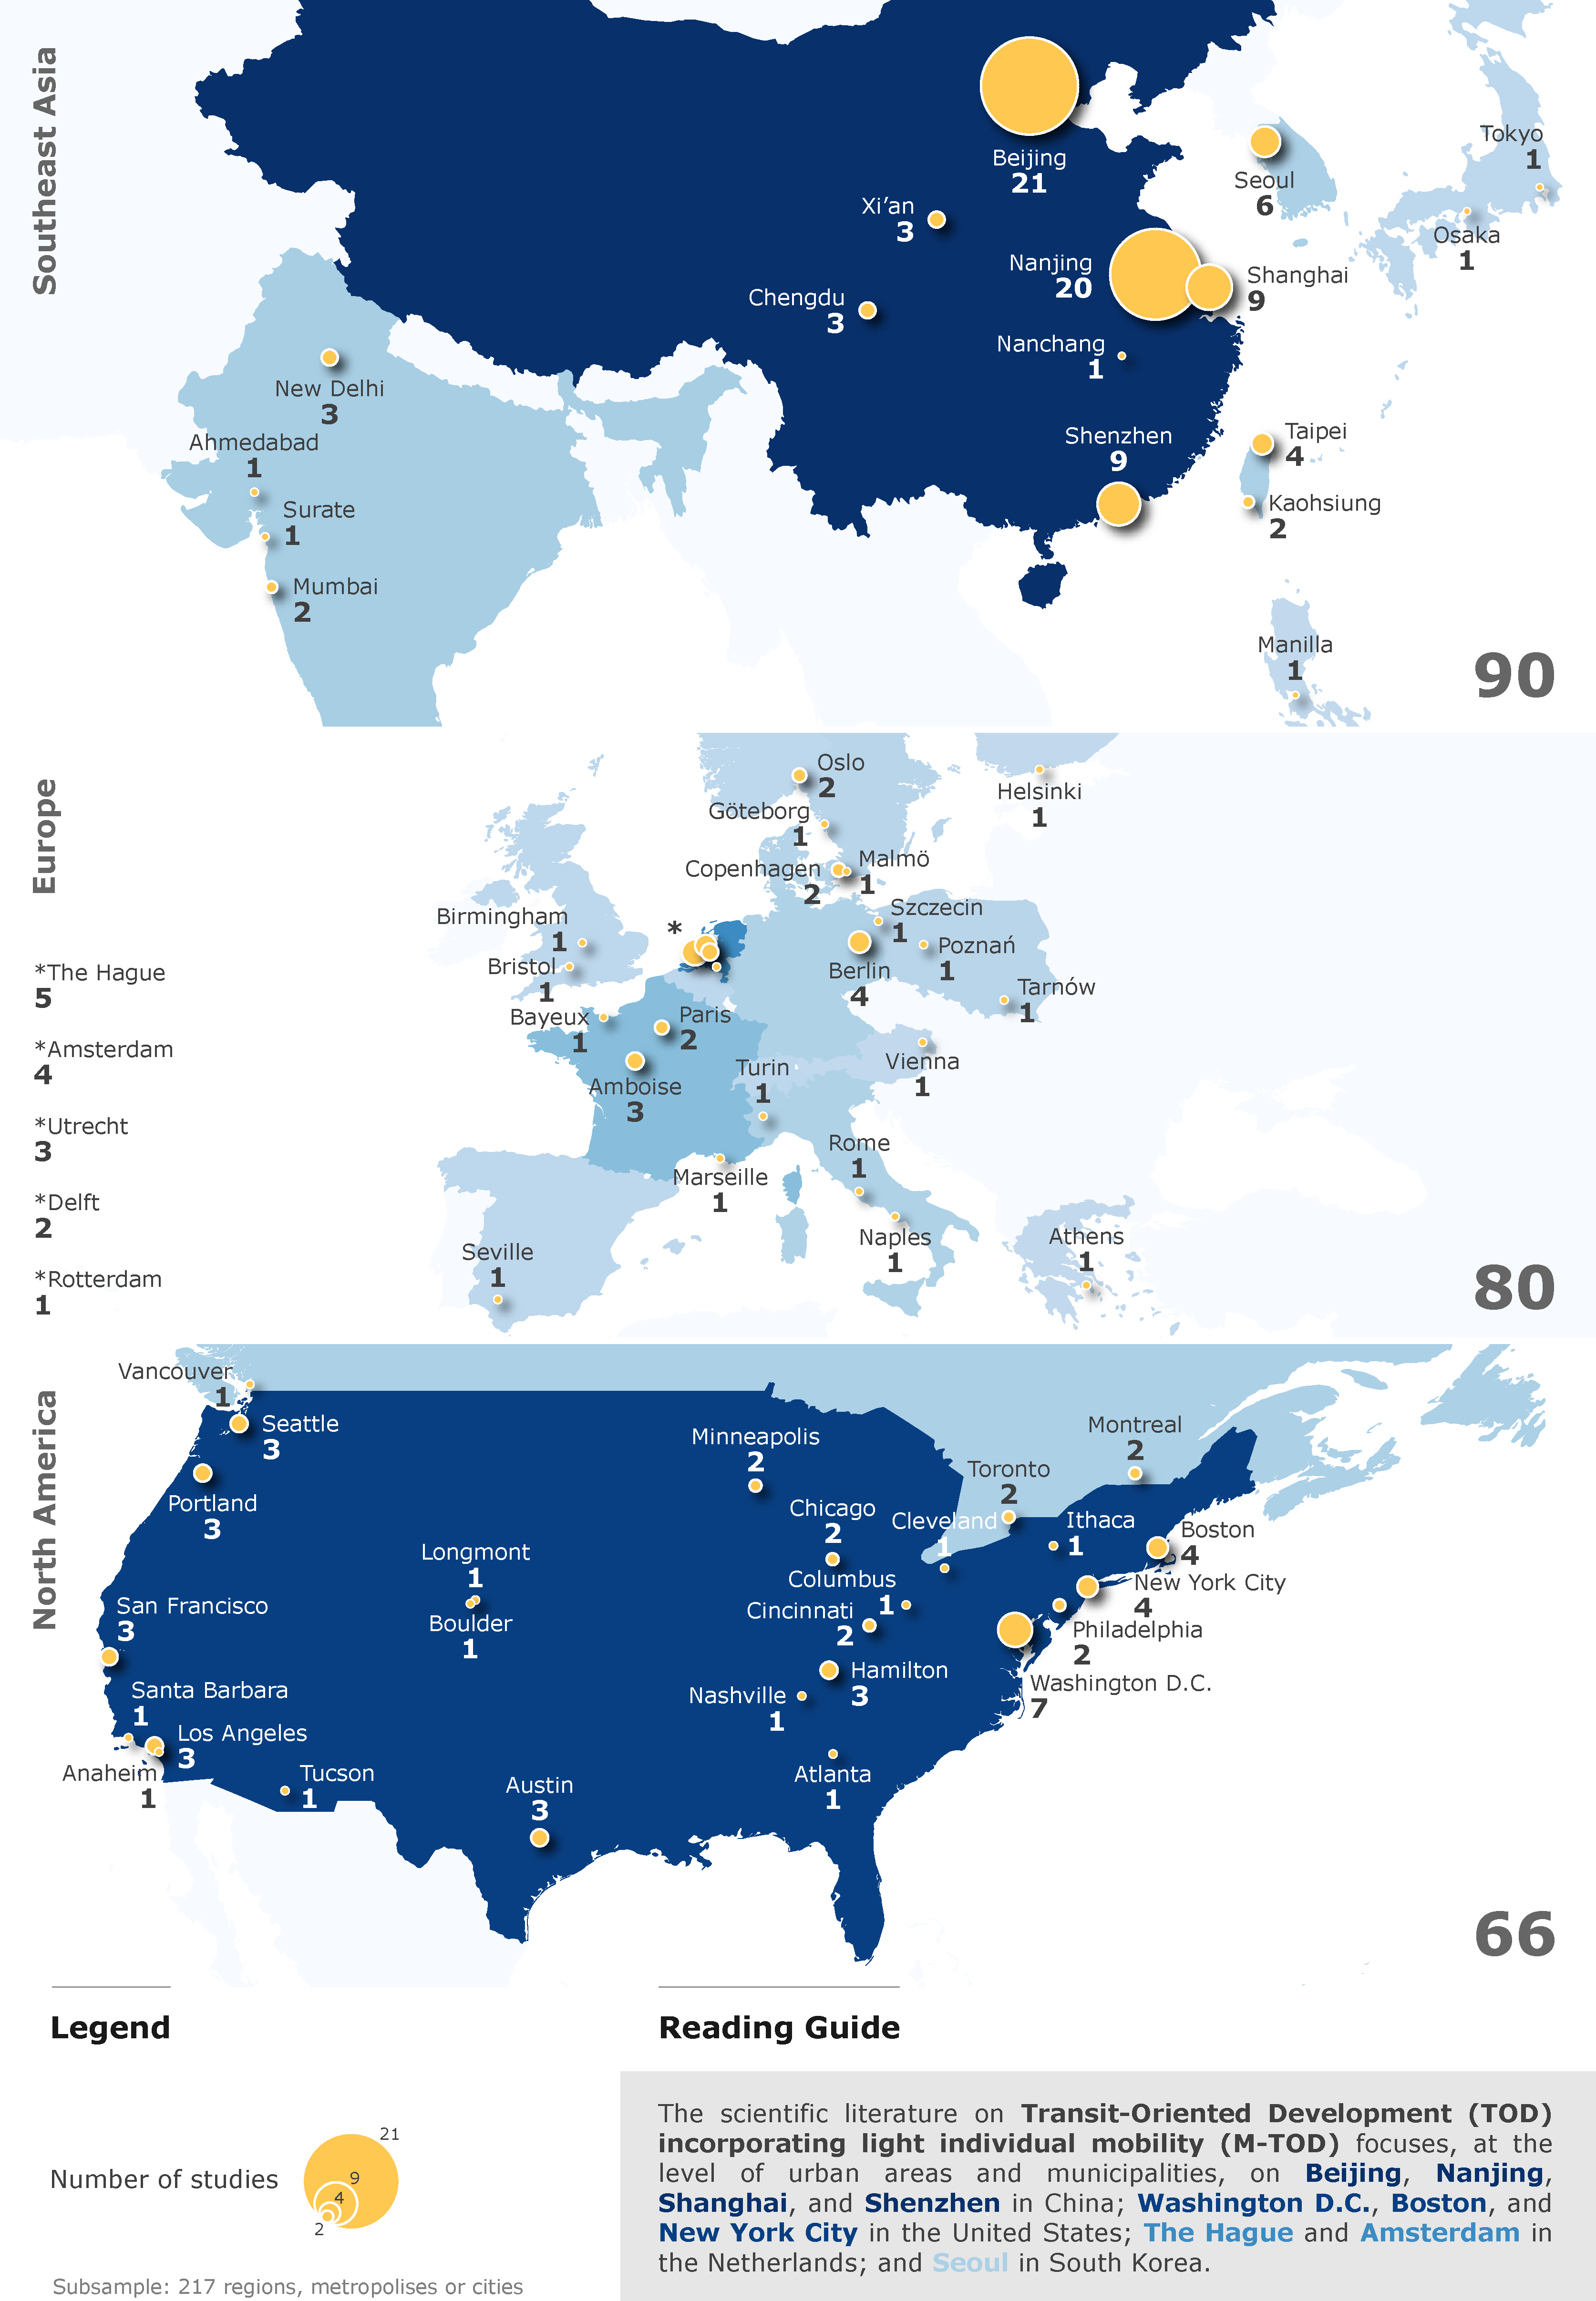
\includegraphics[width=1\columnwidth]{src/Figures/Chap-2/EN_RSL_Carte_Villes.pdf}}
        \vspace{5pt}
        \begin{flushleft}\scriptsize{
        \textcolor{blue}{Note:} The total number of contributions associated with each country and continent may exceed the values specific to each metropolitan area and city due to empirical works that have adopted a national scale.
        }\end{flushleft}
        \begin{flushright}\scriptsize{
        Author: \textcolor{blue}{Dylan Moinse (2023)}
        }\end{flushright}
    \end{carte}

    % micromobility and Public Transport by Continent
A second aspect addressed in this section focuses on the forms of intermodality studied in the analyzed documentation. As shown by the distributions displayed in \hyperref[fig-chap2:MIL-TC-continents]{Map~\ref{fig-chap2:MIL-TC-continents}} (page~\pageref{fig-chap2:MIL-TC-continents}), the various categories of light individual mobility and public transport are investigated unequally, depending on specific geographic areas. First, emerging light individual mobility is much more prominent in Asia, regarding bike-sharing, and in North America, for electric scooter services. Scientific publications selecting European settings primarily focus on conventional bicycles. Second, research on urban public transport systems is also concentrated in Asia, mainly with the metro, and in North America, with metro, tram, and bus systems. On a national scale, some countries specialize in specific forms of intermodality. Regarding bicycles and micromobility, we can particularly highlight the following list of countries:
\begin{customitemize}
    \item In the context of 126 survey sites on personal bicycles, 29 are in the United States, 28 in the Netherlands, 15 in China, 11 in France, 6 in India, and 4 in Canada. Additionally, 3 case studies each are found in South Africa, Germany, Australia, Brazil, Canada, Denmark, and Italy;
    \item Out of 60 locations addressing \acrshort{PBS}, 21 are in China, 17 in the United States, 5 in Taiwan, and 3 each in South Korea and the Netherlands;
    \item Regarding the list of 44 case studies on \acrshort{DBS}, only three countries are involved: 37 are located in China, 5 in the United States, and 2 in the Netherlands;
    \item Among the 20 empirical studies focused on the \acrshort{DESS} system, 13 are concentrated in the United States, and 2 in Germany.
\end{customitemize}
This statistical analysis can be compared with the \acrshort{SLR} conducted by \textcolor{blue}{\textcite[298]{zhang_built_2023}}\index{Zhang, Yushan|pagebf}\index{Kasraian, Dena|pagebf}\index{Wesemael, Pieter van|pagebf} on light individual mobility, which reports a higher proportion of studies on the \acrshort{DESS} system in Europe and on \acrshort{PBS} and \acrshort{DBS} in Asia, explained by the respectively developed markets.%%Translated%%

    % Figure MIL and TC by Continents
    \begin{figure}[h!]\vspace*{4pt}
        \caption{Forms of light individual mobility and public transport evaluated in the systematic literature review, by continent.}
        \label{fig-chap2:MIL-TC-continents}
        \centerline{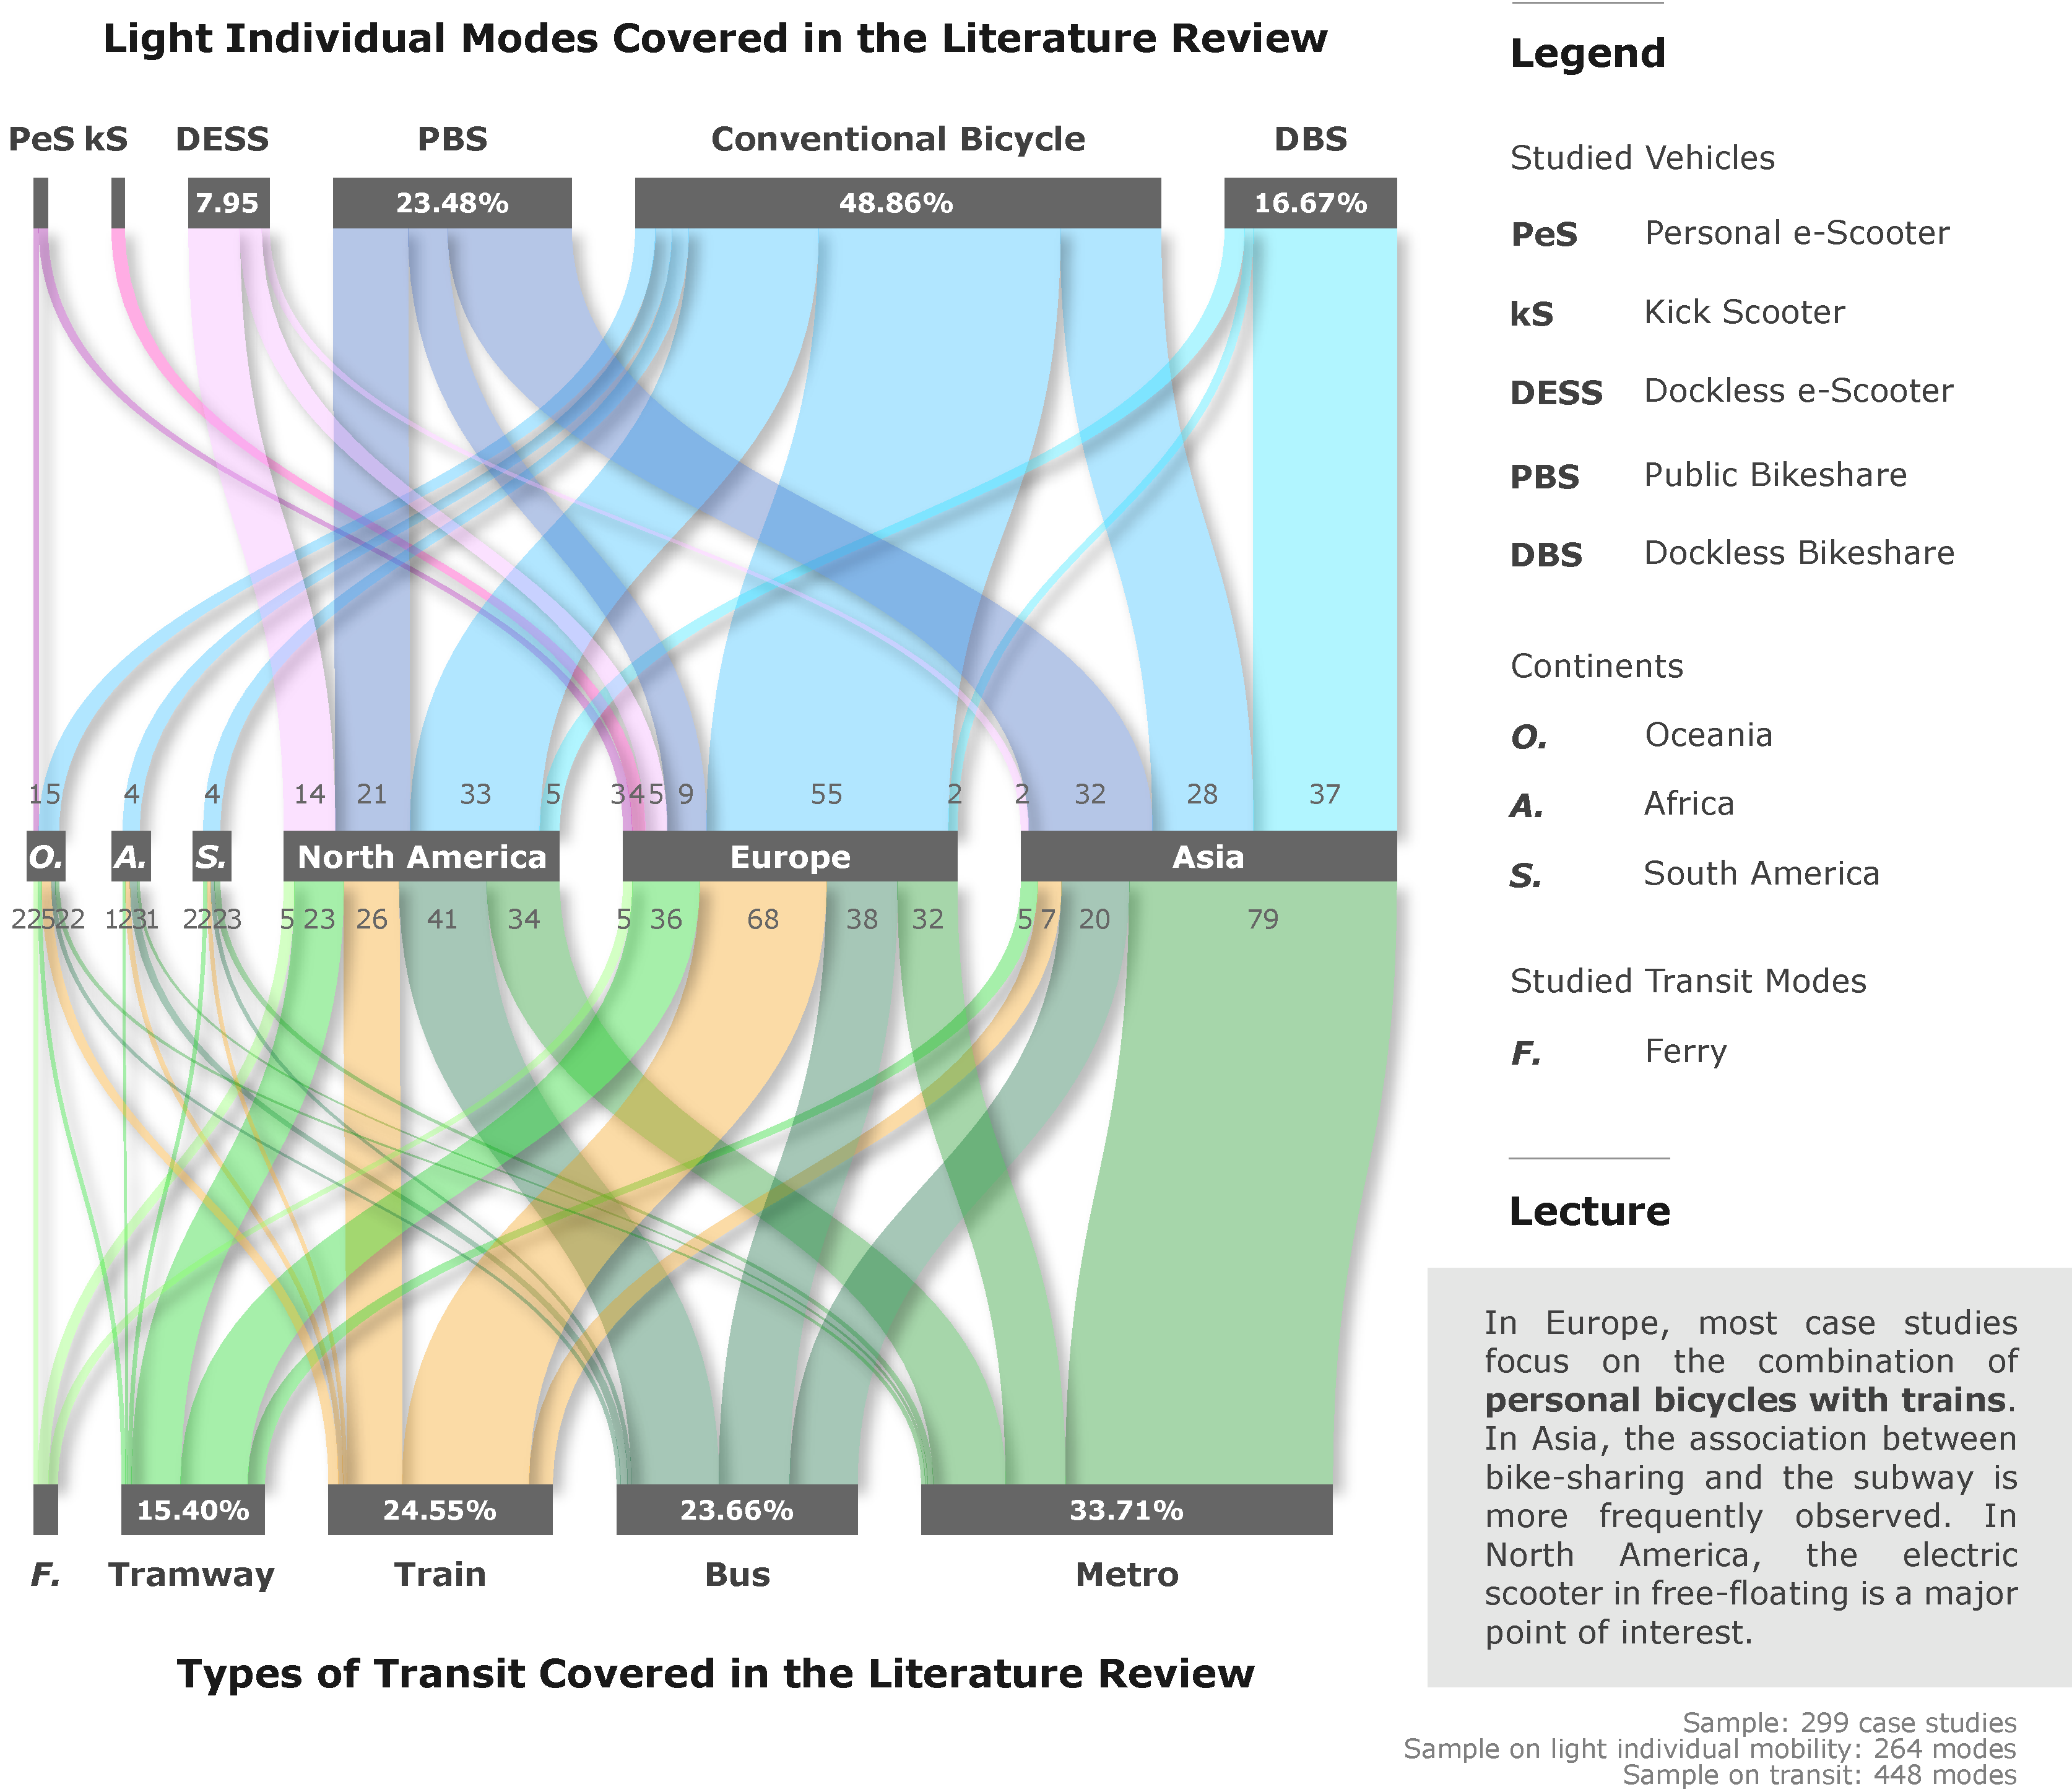
\includegraphics[width=1\columnwidth]{src/Figures/Chap-2/EN_RSL_MIL_TC_Continents.pdf}}
        \vspace{5pt}
        \begin{flushright}\scriptsize{
        Author: \textcolor{blue}{Dylan Moinse (2023)}
        %\\
        %Created with \Marque{Python}~and \Marque{Illustrator}
        }\end{flushright}
    \end{figure}

    % TC Multimodality
    Although the discernible distinction between different public transport systems is ambiguous when it comes to making international comparisons\footnote{~
    The ambiguity between metro and train in the context of international comparisons is inevitable due to geographical, cultural, and transport approach differences. Local trends and preferences, as well as technological and urban development, can blur the lines between metro and train, especially when comparing different regions.
}, a significant proportion of the academic contributions engage in simultaneous investigation of various modes of public transport. It is clear that, among the studies analyzed, the bus is examined in 66 scientific publications, similar to metro (55 occurrences), tram (53 occurrences), and train (51 occurrences), when considered alongside other modes of public transport. As for ferries, this maritime mode is consistently intertwined with other collective modes. Of the 72 documents addressing multiple collective modes simultaneously, 23 refer to the United States, 9 originate from China, and France and the Netherlands each contribute 6 studies.%%Translated%%

    % Minority Countries
As original contributions from regions that have been underexplored or omitted by the \acrshort{SLR}, we should mention the scientific works of \textcolor{blue}{\textcite[34]{bechstein_cycling_2010}}\index{Bechstein, Eva|pagebf}, \textcolor{blue}{\textcite[368]{cooke_relationship_2018}}\index{Cooke, Sean|pagebf}\index{Behrens, Roger|pagebf}\index{Zuidgeest, Mark|pagebf} and \textcolor{blue}{\textcite[2]{risimati_spatial_2021}}\index{Risimati, Brightnes|pagebf}\index{Gumbo, Trynos|pagebf}\index{Chakwizira, James|pagebf} in South Africa; \textcolor{blue}{\textcite[108]{quarshie_integrating_2007}}\index{Quarshie, Magnus|pagebf}\index{Morrison, Gregory~M.|pagebf}\index{Rauch, Sébastien|pagebf} in Ghana; \textcolor{blue}{\textcite[59]{souza_modelling_2017}}\index{Souza, Flavia de|pagebf}\index{La Paix Puello, Lissy|pagebf}\index{Brussel, Mark|pagebf}\index{Orrico, Romulo|pagebf}, \textcolor{blue}{\textcite[36]{arias_molinares_bike_2018}}\index{Arias Molinares, Daniela|pagebf}\index{Florez, Josefina|pagebf} and \textcolor{blue}{\textcite[40]{jansson_almeida_alternativas_2022}}\index{Jansson Almeida, Bárbara|pagebf} in Brazil; \textcolor{blue}{\textcite[206]{cervero_influences_2009}}\index{Cervero, Robert|pagebf}\index{Sarmiento, Olga~L.|pagebf}\index{Jacoby, Enrique|pagebf}\index{Gomez, Luis Fernando|pagebf}\index{Neiman, Andrea|pagebf} in Colombia; \textcolor{blue}{\textcite[6]{arbis_analysis_2016}}\index{Arbis, David|pagebf}\index{Hossein Rashidi, Taha|pagebf}\index{Dixit, Vinayak~V.|pagebf}\index{Vandebona, Upali|pagebf}, \textcolor{blue}{\textcite[2]{weliwitiya_factors_2017}}\index{Weliwitiya, Hesara|pagebf}\index{Rose, Geoff|pagebf}\index{Johnson, Marilyn|pagebf}, \textcolor{blue}{\textcite[396]{weliwitiya_bicycle_2019}}\index{Weliwitiya, Hesara|pagebf}\index{Rose, Geoff|pagebf}\index{Johnson, Marilyn|pagebf} and \textcolor{blue}{\textcite[5]{zhang_make_2023}}\index{Zhang, Mengyuan|pagebf}\index{Lee, Jinwoo Brian|pagebf} in Australia; or \textcolor{blue}{\textcite[17-22]{ensor_forecasting_2010}}\index{Ensor, Matt|pagebf}\index{Slason, Jonathan|pagebf}\index{Vallyon, Chris|pagebf} and \textcolor{blue}{\textcite[56-64]{ensor_mode_2021}}\index{Ensor, Matt|pagebf}\index{Maxwell,~O.|pagebf}\index{Bruce, Oliver|pagebf} in New Zealand.%%Translated%%

    % Chosen Scales/Perimeters (International/National/EPCI)
The focus on the geographical distribution of the study areas brings about an underlying reflection on the geographical scale preferred by empirical studies. Within the bibliographic corpus, comprising a total of 238 scientific works, four of them do not include case studies, instead adopting mathematical modeling approaches. Additionally, seven other studies only present a literature review, contrasting previous empirical research. Thus, 82\% of the research conducted on \acrshort{M-TOD} has chosen a geographical context based on an \acrfull{EPCI}, a municipality, or a local site. The remaining share is split between the national scale, at 11\%, and the regional scale, totaling 6\%\footnote{~
    It should be noted that this categorization only aims to provide a simplified framework for the various geographical scales, divided between national, regional, intercommunal, and municipal levels. However, this approach has limitations, as the delineation of geographical boundaries for a region or agglomeration varies depending on territorial contexts, leading to potential classification errors. For example, in 2019, the Île-de-France region spanned approximately 12,000 square kilometers and hosted 12 million inhabitants, whereas the Greater New York metropolitan area occupies 34,500 square kilometers with over 20 million inhabitants.
}. It is worth noting that the vast majority of state-of-the-art reviews adopt a national scale in order to compare different territories. Similarly, the \acrshort{SLR} by \textcolor{blue}{\textcite[298]{zhang_built_2023}}\index{Zhang, Yushan|pagebf}\index{Kasraian, Dena|pagebf}\index{Wesemael, Pieter van|pagebf} mentions a significant portion of studies on light individual mobility, where the geographical scope does not exceed municipal boundaries, and conversely, there is an almost complete absence of studies at the regional level.%%Translated%%

    % Types of Analyzed Territories 1 (Metropolises)
Further refining the geographical reference scale, it is interesting to note the plurality of agglomerations examined within the \acrshort{SLR}, in terms of their respective sizes. By focusing on the population of urban areas\footnote{~
    The comparative approach to populations is based on demographic data created by \textcolor{blue}{\textcite[]{schiavina_ghs-fua_2019}}\index{Schiavina, Marcello|pagebf}\index{Moreno-Monroy, Ana~I.|pagebf}\index{Maffenini, Luca|pagebf}\index{Veneri, Paolo|pagebf}. This data is grid-based population data that allows defining \acrfull{ZUF} globally \textcolor{blue}{\autocite[3]{moreno-monroy_metropolitan_2021}}\index{Moreno-Monroy, Ana~I.|pagebf}\index{Schiavina, Marcello|pagebf}\index{Veneri, Paolo|pagebf}.
}, we observe the three predominant continents in the study of \acrshort{M-TOD}. As shown in \hyperref[table-chap2:tailles-territoires-rsl]{Table~\ref{table-chap2:tailles-territoires-rsl}} (page~\pageref{table-chap2:tailles-territoires-rsl}), megacities\footnote{~
    \Commas{Megacities are urban agglomerations that, according to the United Nations' terminology, concentrate populations of 10 million inhabitants or more.} \textcolor{blue}{\autocite[]{geoconfluences_megapole_2023}}\index{Géoconfluences@\textsl{Géoconfluences}|pagebf}
} with populations over ten million people make up 43\% of the geographical areas present in the \acrshort{SLR}. This ranking is influenced by studies conducted in China (72\%) and, more generally, in East and Southeast Asia (88\%). Similarly, metropolises with international influence and populations exceeding three million inhabitants occupy a significant place in empirical research (27\%). These urban centers are mainly located in the United States (44\%) and specifically in North America (52\%). This phenomenon also echoes among metropolises of national or even international importance with populations over one million. These intermediate metropolises are notably found in Western Europe, making up 44\%, and are predominant when extending the scope to the entire European continent (62\%). Thus, the three types of urban areas mentioned encompass over 87\% of the investigations analyzed in the \acrshort{SLR}.%%Translated%%

    % Tableau types de territoires analysés RSL
% Table of analyzed territories RSL
%%Translated%%
        \begin{table}[h!]
    \centering
    \renewcommand{\arraystretch}{1.5}
    \resizebox{\columnwidth}{!}{
    \begin{tabular}{p{1\columnwidth}}
        %\hline
    \rule{0pt}{15pt} \small{\textbf{\textcolor{blue}{Agglomerations and Municipalities}}}\\
        \hline
    \small{\textbf{\textcolor{blue}{More than 10,000,000 inhabitants (88 references)}}}\\
\small{Beijing (21), Nanjing (19), Shenzhen (9), Shanghai (9), Seoul (6), New York City (4), Chengdu (3), Los Angeles (3), New Delhi (3), Xi'an (3), Chicago (2), Île-de-France (2), Mumbai (2), Bogotá (1), Johannesburg-Pretoria (1), Osaka (1), Manila (1), Rio de Janeiro (1)}\\
        \hdashline
    \small{\textbf{\textcolor{blue}{Between 3,000,000 and 10,000,000 inhabitants (53 references)}}}\\
\small{Washington D.C. (7), Berlin (4), Boston (4), Taipei (4), San Francisco (3), Seattle (3), Suzhou (3), Kaohsiung (2), Melbourne (2), Minneapolis (2), Montreal (2), Philadelphia (2), Toronto (2), Accra (1), Ahmedabad (1), Athens (1), Atlanta (1), Birmingham (1), Boulder (1), Cape Town (1), Nanchang (1), Porto Alegre (1), Rome (1), Surat (1), Sydney (1), Vienna (1)}\\
        \hdashline
    \small{\textbf{\textcolor{blue}{Between 1,000,000 and 3,000,000 inhabitants (33 references)}}}\\
\small{Rotterdam-The Hague (6), Amsterdam (4), Austin (3), Cincinnati (2), Cleveland (2), Copenhagen (2), Oslo (2), Auckland (1), Bristol (1), Columbus (1), Helsinki (1), Gutenberg (1), Aix-Marseille-Provence (1), Nashville (1), Orlando (1), Poznań (1), Seville (1), Tucson (1), Turin (1)}\\
        \hdashline
    \small{\textbf{\textcolor{blue}{Between 250,000 and 1,000,000 inhabitants (16 references)}}}\\
\small{Hamilton (3), Portland (3), Utrecht (3), Delft (2), Amstelland-Meerlanden (1), Eindhoven (1), Malmö (1), Mamelodi (1), Tarnow (1)}\\
        \hdashline
    \small{\textbf{\textcolor{blue}{Less than 250,000 inhabitants (8 references)}}}\\
\small{Amboise (3), Bayeux (1), El Monte (1), Ithaca (1), Longmont (1), Belgian municipalities between 30,000 and 200,000 inhabitants (1)}\\
        \hline
        \end{tabular}}
    \caption{Size of agglomerations and municipalities studied in the systematic literature review.}
    \label{table-chap2:tailles-territoires-rsl}
        \vspace{5pt}
        \begin{flushleft}\scriptsize{
        \textcolor{blue}{Reading:} Based on 198 studies including a geographical area, the systematic literature review primarily consists of agglomerations with more than 3,000,000 inhabitants.
        }\end{flushleft}
        \begin{flushright}\scriptsize
        Author: \textcolor{blue}{Dylan Moinse (2023)}
        \end{flushright}
        \end{table}%%Translated%%

% Types of territories analyzed 2 (regional metropolises)
For agglomerations with populations of less than one million inhabitants, the case studies in urban areas are primarily focused on Dutch intermunicipalities, specifically in the localities of Delft \textcolor{blue}{\autocites[113]{heinen_multimodal_2014}[5]{molin_bicycle_2015}}\index{Heinen, Eva|pagebf}\index{Bohte, Wendy|pagebf}\index{Molin, Eric|pagebf}\index{Maat, Kees|pagebf}, Amstelland-Meerlanden \textcolor{blue}{\autocite[46]{brand_assessing_2015}}\index{Brand, Judith Caroline|pagebf}, Eindhoven \textcolor{blue}{\autocite[724]{waerden_relation_2018}}\index{Waerden, Peter|pagebf}\index{Waerden, Jaap|pagebf}, and Utrecht \textcolor{blue}{\autocite[289]{kuijk_preferences_2022}}\index{Mil, Joeri~F.P. van|pagebf}\index{Leferink, Tessa~S.|pagebf}\index{Annema, Jan Anne|pagebf}\index{Oort, Niels van|pagebf}\index{Kuijk, Roy~J. van|pagebf}\index{Almeida Correia, Gonçalo Homem de|pagebf}\index{Oort, Niels van|pagebf}\index{Arem, Bart van|pagebf}. The United States also constitutes a relevant area for this research topic, with studies based in Portland \textcolor{blue}{\autocites[164]{krizek_assessing_2011}[400]{mcqueen_assessing_2022}[94]{singleton_exploring_2014}[265]{welch_long-term_2016}[83]{pucher_integrating_2009}}\index{Krizek, Kevin~J.|pagebf}\index{Stonebraker, Eric~W.|pagebf}\index{McQueen, Michael|pagebf}\index{Clifton, Kelly~J.|pagebf}\index{Singleton, Patrick~A.|pagebf}\index{Welch, Timothy~F.|pagebf}\index{Gehrke, Steven~R.|pagebf}\index{Wang, Fangru|pagebf}\index{Pucher, John|pagebf}\index{Buehler, Ralph|pagebf} and Anaheim, in the Greater Los Angeles Area \textcolor{blue}{\autocite[1579]{liu_simultaneous_2015}}\index{Liu, Yang|pagebf}\index{Zhu, Ning|pagebf}\index{Ma, Shou-feng|pagebf}. Similarly, Canadian territories contribute to this body of work, with scientific publications focused on the metropolitan area of Hamilton \textcolor{blue}{\autocites[2162]{chan_factors_2020}[375]{ravensbergen_biking_2018}}\index{Ravensbergen, Léa|pagebf}\index{Chan, Kevin|pagebf}\index{Farber, Steven|pagebf}\index{Buliung, Ron|pagebf}\index{Mendonca, Meaghan|pagebf}\index{Garg, Naren|pagebf}. As for rural and suburban territorial arrangements, French examples are numerous, marked by a series of studies conducted in the municipalities of Amboise \textcolor{blue}{\autocites[747]{midenet_modal_2018}[2729]{papon_evaluation_2017}[14-16]{papon_rapport_2015}}\index{Midenet, Sophie|pagebf}\index{Côme, Etienne|pagebf}\index{Papon, Francis|pagebf}\index{Beauvais, Jean-Marie|pagebf}\index{Midenet, Sophie|pagebf}\index{Côme, Etienne|pagebf}\index{Polombo, Nadine|pagebf}\index{Abours, Sylvie|pagebf}\index{Belton-Chevallier, Leslie|pagebf}\index{Soulas, Claude|pagebf} and Bayeux \textcolor{blue}{\autocite[2]{richer_service_2017}}\index{Richer, Cyprien|pagebf}, as well as in the former \acrfull{CC} of the Brie Boisée (now part of Île-de-France since 2017), in comparison with that of Carnelle Pays de France and Haute Vallée de Chevreuse \textcolor{blue}{\autocite[39]{stransky_periurbain_2019}}\index{Stransky, Vaclav|pagebf}.%%Translated%%

% International comparisons figure
\begin{figure}[h!]\vspace*{4pt}
    \caption{Comparisons between geographical areas in the bibliographic corpus of the systematic literature review.}
    \label{fig-chap2:comparaisons-internationales-rsl}
    \centerline{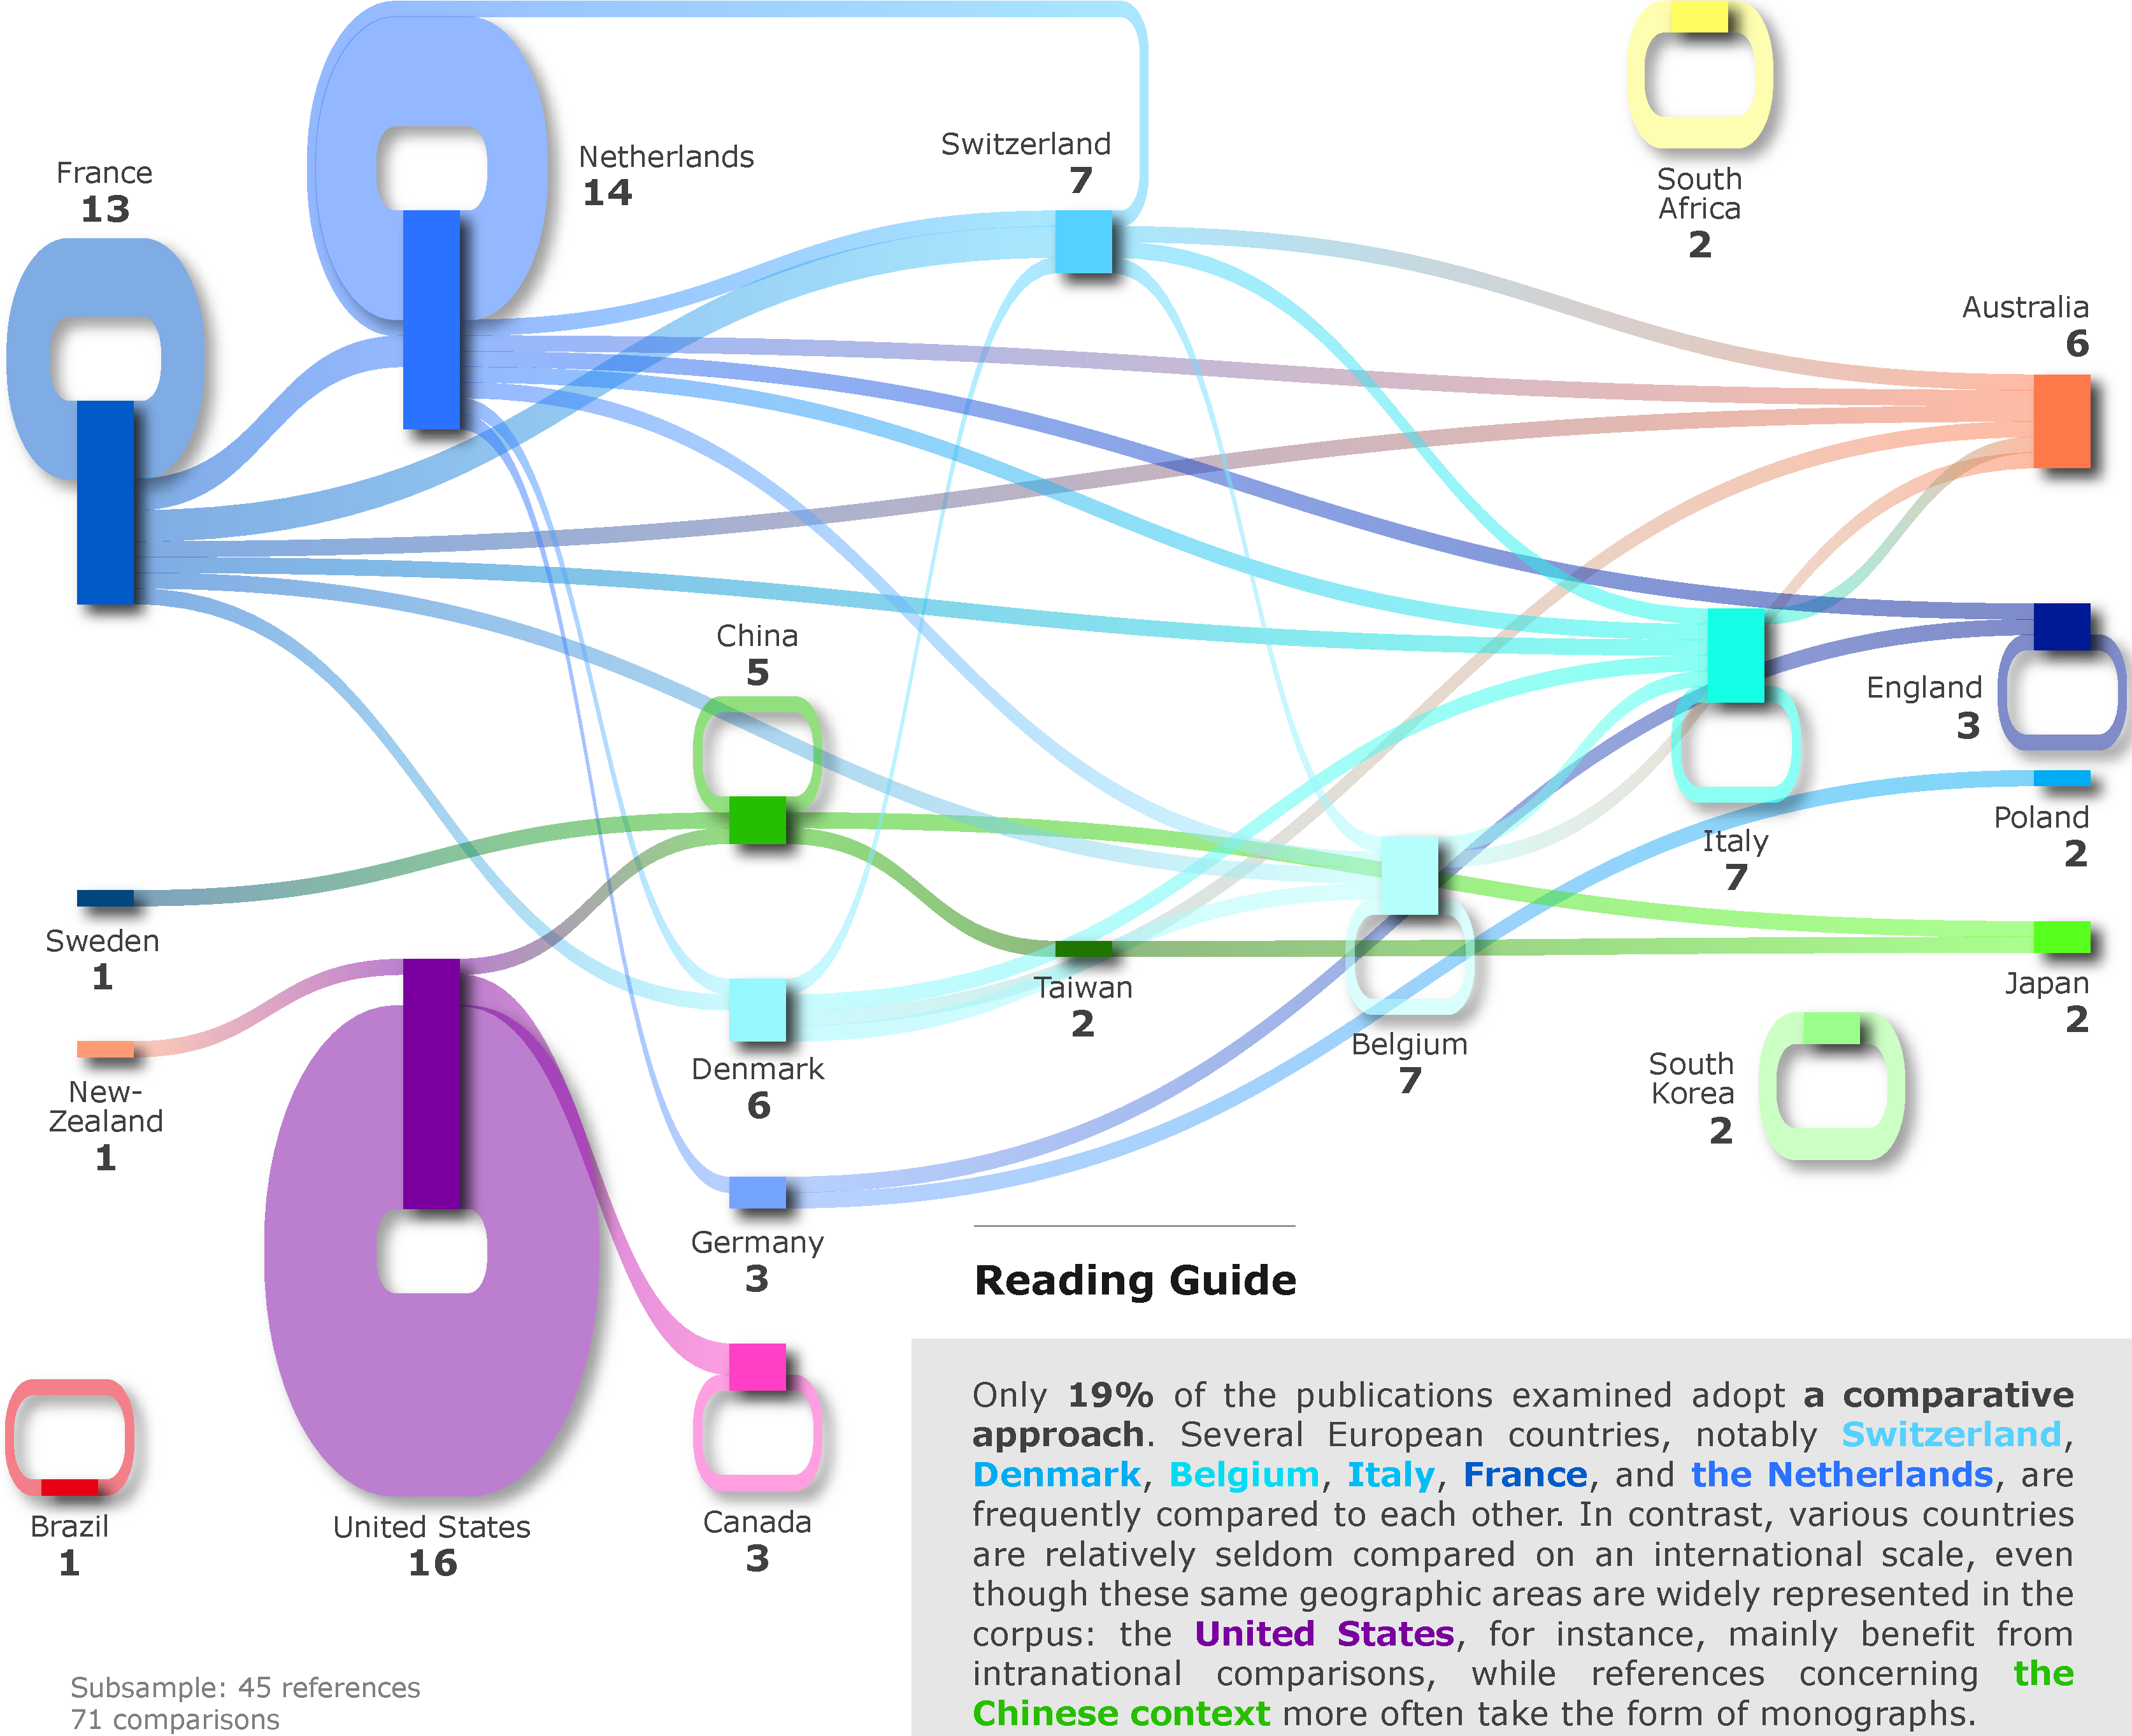
\includegraphics[width=1\columnwidth]{src/Figures/Chap-2/EN_RSL_Comparaisons_internationales.pdf}}
    \vspace{5pt}
    \begin{flushright}\scriptsize{
    %\\
    %Created with \Marque{Python}~and \Marque{Illustrator
    \textcolor{blue}{Note:} Only comparisons between different regions were considered in order to exclude urban areas with multiple local sites studied. The ring represents subnational comparisons, while the flows link the geographical areas in perspective.
    \\
    Author: \textcolor{blue}{Dylan Moinse (2023)}
    }\end{flushright}
\end{figure}

% International comparisons
While the literature on \acrshort{M-TOD} commonly adopts a comparative approach by selecting various study sites within a coherent political system, fewer studies make parallel comparisons between territories in different countries. In fact, it appears that 19\% of the publications reviewed focus on international or subnational comparisons. In the subset of 45 scientific papers dedicated to comparisons, 30 of them make comparisons between different \acrshort{EPCI}, while 11 others focus on the national level. As shown in \hyperref[fig-chap2:comparaisons-internationales-rsl]{Figure~\ref{fig-chap2:comparaisons-internationales-rsl}} (page~\pageref{fig-chap2:comparaisons-internationales-rsl}), certain countries are frequently compared, such as Switzerland, Denmark, Belgium, Italy, France, and the Netherlands \textcolor{blue}{\autocites[29-46]{abours_rapport_2015}[279-285]{sebban_complementarite_2003}[282-284]{martens_bicycle_2004}}\index{Abours, Sylvie|pagebf}\index{Midenet, Sophie|pagebf}\index{Soulas, Claude|pagebf}\index{Sebban, Annie-Claude|pagebf}\index{Martens, Karel|pagebf}, often with other European countries; or Japan, Taiwan, and China \textcolor{blue}{\autocite[212]{lin_built_2018}}\index{Lin, Jen-Jia|pagebf}\index{Zhao, Pengjun|pagebf}\index{Takada, Kazuyuki|pagebf}\index{Li, Shengxiao|pagebf}\index{Yai, Tetsuo|pagebf}\index{Chen, Chi-Hao|pagebf}. It is worth noting that there are also two intercontinental comparisons, conducted by \textcolor{blue}{\textcite[4]{hamidi_shaping_2020}}\index{Hamidi, Zahra|pagebf}\index{Zhao, Chunli|pagebf} who studied the urban areas of Beijing, Göteborg, and Malmö in China and Sweden; and by \textcolor{blue}{\textcite[13]{hua_transfer_2022}}\index{Hua, Mingzhuang|pagebf}\index{Pereira, Francisco Camara|pagebf}\index{Jiang, Yu|pagebf}\index{Chen, Xuewu|pagebf} who examined the Chinese and U.S. cities of Nanjing and Chicago.%%Translated%%

% Subnational comparisons
In contrast, some countries are rarely put into perspective, even though they are occasionally compared in small proportions (see \hyperref[fig-chap2:comparaisons-internationales-rsl]{Figure~\ref{fig-chap2:comparaisons-internationales-rsl}}, page~\pageref{fig-chap2:comparaisons-internationales-rsl}). For instance, the United States, except for some comparisons with Canada \textcolor{blue}{\autocites[11-16]{ensor_forecasting_2010}[7]{schneider_integration_2005}[83]{pucher_integrating_2009}}\index{Ensor, Matt|pagebf}\index{Slason, Jonathan|pagebf}\index{Vallyon, Chris|pagebf}\index{Schneider, Robert|pagebf}\index{Pucher, John|pagebf}\index{Buehler, Ralph|pagebf}, mainly benefit from subnational comparisons. Some countries have only been involved in internal comparisons between different regions within the same geographical entity. In South Africa, \textcolor{blue}{Eva} \textcolor{blue}{\textcite[34]{bechstein_cycling_2010}}\index{Bechstein, Eva|pagebf} conducts a comparative study between the \Commas{\textsl{townships}}\footnote{~
    \Commas{In South Africa, since the \textsl{apartheid} regime, the term \textsl{township} refers to areas inhabited by people of color (black and \textsl{coloured}). [\dots] Over time, the term has come to describe poor, degraded, and unsanitary housing areas, approaching the definition of a slum.} \textcolor{blue}{\autocite{geoconfluences_township_2023}}\index{Géoconfluences@\textsl{Géoconfluences}|pagebf}.
} of Mamelodi and Nellmapius (Tshwane), similarly to \textcolor{blue}{\textcite[368]{cooke_relationship_2018}}\index{Cooke, Sean|pagebf}\index{Behrens, Roger|pagebf}\index{Zuidgeest, Mark|pagebf} who compare the metropolitan municipalities of Johannesburg, Cape Town, Tshwane, Nelson Mandela Bay, and eThekwini. In South Korea, research by \textcolor{blue}{\textcite[43, 980]{lee_strategies_2010, lee_bicycle-based_2016}}\index{Lee, Jaeyeong|pagebf}\index{Shin, Hee-Cheol|pagebf}\index{Lee, Jaeyeong|pagebf}\index{Choi, Keechoo|pagebf}\index{Leem, Yountaik|pagebf} focuses on a comparative analysis between the metropolitan regions of Seoul and Daejeon.%%Translated

% Few comparisons
In contrast, \hyperref[fig-chap2:comparaisons-internationales-rsl]{Figure~\ref{fig-chap2:comparaisons-internationales-rsl}} (page~\pageref{fig-chap2:comparaisons-internationales-rsl}) reveals the underrepresentation, or even absence, of certain countries that are well-studied in the \acrshort{SLR}. The most striking case is that of China, where the vast majority of research uses a monographic approach, focusing solely on a single agglomeration. However, it should be noted that these studies are not necessarily non-comparative \textcolor{blue}{\autocite[30-31]{gueranger_monographie_2012}}\index{Guéranger, David|pagebf}. For example, the study conducted by \textcolor{blue}{\textcite[77]{liu_solving_2012}}\index{Liu, Zhili|pagebf}\index{Jia, Xudong|pagebf}\index{Cheng, Wen|pagebf} carries out two case studies in the districts of Dongcheng and Haidian, in Beijing, after conducting an exhaustive analysis of the \acrshort{PBS} system around subway and bus stops in the capital. By excluding comparisons within the same urban area due to methodological constraints related to the normalization of geographical areas, this chart masks the analogical reasoning present at the submunicipal level.%%Translated%%

% Conclusion
In summary, this section dedicated to the state of international scientific literature on \acrshort{M-TOD} has examined both the analysis of the metadata of the collected scientific publications, the lexical patterns used to describe the research topic, as well as the chronological trends and the geographical distribution of the investigations conducted. After analyzing the documentation from the metadata perspective, the following section will address the conceptual and methodological frameworks of the scientific literature on \acrshort{M-TOD}, focusing on the theoretical foundations, the evaluation of approaches, and the types of analysis employed in the investigations.%%Translated%%

% 2.2.2. Concepts, methods, types of analysis
\needspace{1\baselineskip} % Reserve space
\subsection{Conceptual and Methodological Frameworks of the Corpus
    \label{chap2:cadres-conceptuels-methodologiques}
    }

% Introduction
This section is dedicated to presenting and comparing the various theoretical foundations and approaches used in the scientific literature. The following questions have been considered in this analysis:
    \begin{customitemize}
        \item What are the main theoretical frameworks employed in the selected documentation? How have these theoretical choices been applied to the research questions?
        \item Can we identify any evolution of the theoretical frameworks adopted over time? Do these trends reflect certain disciplinary directions or advancements? What criticisms have the authors raised regarding the theoretical frameworks used?
        \item What data collection methods have been used? What data analysis techniques have been applied?
        \item How have the authors addressed the constraints and limitations of the data collection and analysis methods used?
    \end{customitemize}%%Translated%%

% Plan announcement
This subsection aims to introduce the theoretical frameworks found in the scientific literature (\hyperref[chap2:fondements-theoriques]{Subsection~2.2.1}, page~\pageref{chap2:fondements-theoriques}), prior to evaluating the data collection processes (\hyperref[chap2:methodes-collecte-donnees]{Subsection~2.2.2}, page~\pageref{chap2:methodes-collecte-donnees}) and the data analysis methods (\hyperref[chap2:demarches-types-analyses]{Subsection~2.2.3}, page~\pageref{chap2:demarches-types-analyses}) employed to study \acrshort{M-TOD}.%%Translated%%

% 2.2.2.1. Mobilized Concepts, TOD
\needspace{1\baselineskip} % Reserve space
\subsubsection*{Theoretical Foundations
    \label{chap2:fondements-theoriques}
    }

% Theoretical frameworks description
In the 102 scientific articles analyzed in the context of the \acrshort{SLR}, the concept of \acrshort{TOD} is predominant, being cited in 55 studies. Among these, 53 articles explicitly discuss \acrshort{TOD}, with nine of them specifically relying on the principles of the \Commas{Ds} to structure their analysis. Four studies are based on an analytical approach of the \Commas{5Ds}, three on the \Commas{3Ds}, one on the \Commas{4Ds}, and another on the \Commas{6Ds}\footnote{~
    In the commonly accepted order in the scientific literature on \acrshort{TOD}, and as presented in the \hyperref[chap1:tod-presentation-generale-definition]{section on the definition of \textsl{Transit-Oriented Development}} (page~\pageref{chap1:tod-presentation-generale-definition}) of \hyperref[chap1:titre]{Chapter~1} (page~\pageref{chap1:titre}), the \Commas{\acrshort{7Ds}} are composed as follows: Density (\(D1\)), Diversity (\(D2\)), Design (\(D3\)), Destination Accessibility (\(D4\)), Distance to Transit (\(D5\)), Demand Management (\(D6\)), and Demographics (\(D7\)).
}. Four articles integrate a revised version of \acrshort{TOD} that closely reflects this chapter, focusing on \acrshort{M-TOD}. The significant place of \acrshort{TOD} in the literature is, however, influenced by its inclusion in our research formula during the database collection. In addition to \acrshort{TOD}, two other concepts frequently emerge: the \Commas{first and last miles,} mentioned 24 times, and \Commas{multimodal accessibility,} discussed in 20 articles. Other concepts are also present, such as \Commas{car dependency} (four mentions), \acrfull{MaaS} (four mentions), \Commas{social inclusivity} (four mentions), and \Commas{planned behavior theory} (two mentions).%%Translated%%

% Focus on M-TOD
In fact, a significant number of publications address the concept of \acrshort{TOD} without explicitly mentioning it. Similarly, although rarely cited, the concept of \acrshort{M-TOD} is intrinsically linked to the academic corpus that examines the integration of light individual mobility with public transport networks, while articulating issues related to mobility and urban development. First, it is worth mentioning the study by \textcolor{blue}{\textcite{lee_bicycle-based_2016}}\index{Lee, Jaeyeong|pagebf}\index{Choi, Keechoo|pagebf}\index{Leem, Yountaik|pagebf} that led to the conceptualization of \acrshort{B-TOD}, based on an investigation exploring the relationship between bicycles and the subway in Seoul and Daejeon. Additionally, three studies using \acrshort{B-TOD} focus on different objects and geographical contexts: one in Nanjing examining bicycles, \acrshort{PBS}, and the subway \textcolor{blue}{\autocite{ji_public_2017}}\index{Ji, Yanjie|pagebf}\index{Fan, Yingling|pagebf}\index{Ermagun, Alizera|pagebf}\index{Cao, Xuening|pagebf}\index{Wang, Wei|pagebf}\index{Das, Kirti|pagebf}; another in Kaohsiung between \acrshort{PBS} and the subway \textcolor{blue}{\autocite{cheng_expanding_2018}}\index{Cheng, Yung-Hsiang|pagebf}\index{Li, Yi-Chun|pagebf}; and the last studying the link between bicycles and buses in the cities of Cape Town, Tshwane, Joburg, Nelson Mandela Bay, and eThekwini \textcolor{blue}{\autocite{cooke_relationship_2018}}\index{Cooke, Sean|pagebf}\index{Behrens, Roger|pagebf}\index{Zuidgeest, Mark|pagebf}. The diversity of theoretical approaches adopted reflects the methodological plurality aimed at exploring the interactions between bicycles, micromobility, and public transport.%%Translated%%

% 2.2.2.2. Methods, data sources, and sample
\needspace{1\baselineskip} % Reserve space
\subsubsection*{Evaluation of Data Collection Methods
    \label{chap2:methodes-collecte-donnees}
    }

% Detailed data sources: big data
The analysis of the data sources used in the documentation led to the identification of 17 types of data collection methods, classified into five independent categories. The majority of the scientific productions rely on the use of open data (29.15\%) and usage data (23.87\%), which can be grouped under the technical concept of \textsl{Big Data}\footnote{~
    In the context of mobility, \textsl{Big Data} refers to the collection and processing of a public or private database generated by a transport system, vehicle, users themselves, or other available sources. This technique for collecting real-time quantitative data is made possible by the emergence of technologies such as sensors embedded in vehicles, counters, smartphones, or the deployment of digital tools.
}, followed by surveys (24.62\%) and secondary data analysis from databases (16.58\%). The mobility flows available online thus represent 53.02\% of the data sources used and primarily correspond to \textsl{Open Data}\footnote{~
    \textsl{Open Data} refers, in the case of this \acrshort{SLR}, to the public data-sharing policy related to urban planning and mobility. These open data, provided by local authorities and public agencies, include various information related to urban planning, land use, infrastructure, demographics, and other aspects of territorial management.
} (22.54\%), \acrfull{API}\footnote{~
    An \acrshort{API} is a computer interface that connects applications and services with mobility systems in a standardized manner. \acrshort{API}\textcolor{blue}{s} facilitate the exchange of data between mobility service providers and third-party applications, such as vehicle location, status, and availability in real-time, unlocking vehicles, and the billing process for a trip made. All the data generated and exchanged allow companies to access aggregated data on vehicle usage and integrate it.
} (11.72\%), and mobility flows related to \acrshort{PBS} systems, called \acrfull{GBFS}\footnote{~
    \acrshort{GBFS} defines a standardized data format specifically designed for \acrshort{PBS} systems, aimed at providing real-time information about the mobility service and promoting interoperability and transparency.
} (9.02\%) and public transport, \acrfull{GTFS}\footnote{~
    \acrshort{GTFS} is a standardized file format, initially called the \Commas{\textsl{Google Transit Feed Specification}}, used to describe public transport networks. This includes routes, stop points, time schedules, and ridership data. This standardization aims to facilitate the integration of these open data into mapping and route planning tools. For this purpose, public transport agencies provide these standardized formats, targeting both third-party application developers and users.
} (6.85\%). We also find some data collection techniques classified under open and usage data, such as extracting mobility data from multimodal maps, around 2.16\%, or \acrshort{GPS} data (\textsl{Global Positioning System}), at 1.89\%.%%Translated%%

% Detailed data sources: qualitative methods
Beyond this data collection method related to \textsl{Smart Data}, a second range emerges associated with field surveys, through questionnaires (20.47\%), interviews (2.80\%), and observations (1.98\%). These techniques, rooted in the research practices of geography and sociology, are driven by the implementation of online questionnaires (11.45\%), face-to-face (7.66\%), and postal (1.35\%) surveys, as well as individually (1.71\%) or collectively (1.08\%) conducted interviews and direct observation sessions (1.98\%). The plurality of data collection methods is lastly reflected in the exploitation and reinterpretation of pre-existing public surveys (14.52\%) and the synthesis of previous materials (0.81\%).%%Translated%%

% Data sources by continent
By intertwining the data collection and processing methods used in scientific productions with the geographical context of the areas examined, differences in the use of data sources emerge (see \hyperref[fig-chap2:sources-donnees-rsl]{Figure~\ref{fig-chap2:sources-donnees-rsl}}, page~\pageref{fig-chap2:sources-donnees-rsl}). In this regard, we observe that Asian territories show a marked propensity for exploiting open data and usage data. This trend is more specifically manifested through the use of digital data from geographical sources, such as \textsl{Open Data}, \acrshort{API}, \acrshort{GBFS}, and multimodal maps\footnote{~
    A multimodal card, or \textsl{Smart Card}, refers to a card that integrates and displays information about several different transport modes within a single interface. By combining this information into one card, it can automatically collect anonymous data on user movements across a transport network, generally integrating train systems, urban public transport, and \acrshort{PBS}.
}. Similarly, online questionnaire surveys stand out for their prevalence across the three considered continents, whereas face-to-face questionnaires are more commonly used in Asian contexts. In parallel, interviews and observations, as well as secondary analysis of public surveys and literature reviews, are approaches more pronounced in North America and Europe.%%Translated%%

% Figure data sources RSL
\begin{figure}[h!]\vspace*{4pt}
    \caption{An imbalanced use of data collection methods according to geographical contexts, urban size, and the type of light individual mobility studied in the systematic literature review.}
    \label{fig-chap2:sources-donnees-rsl}
    \centerline{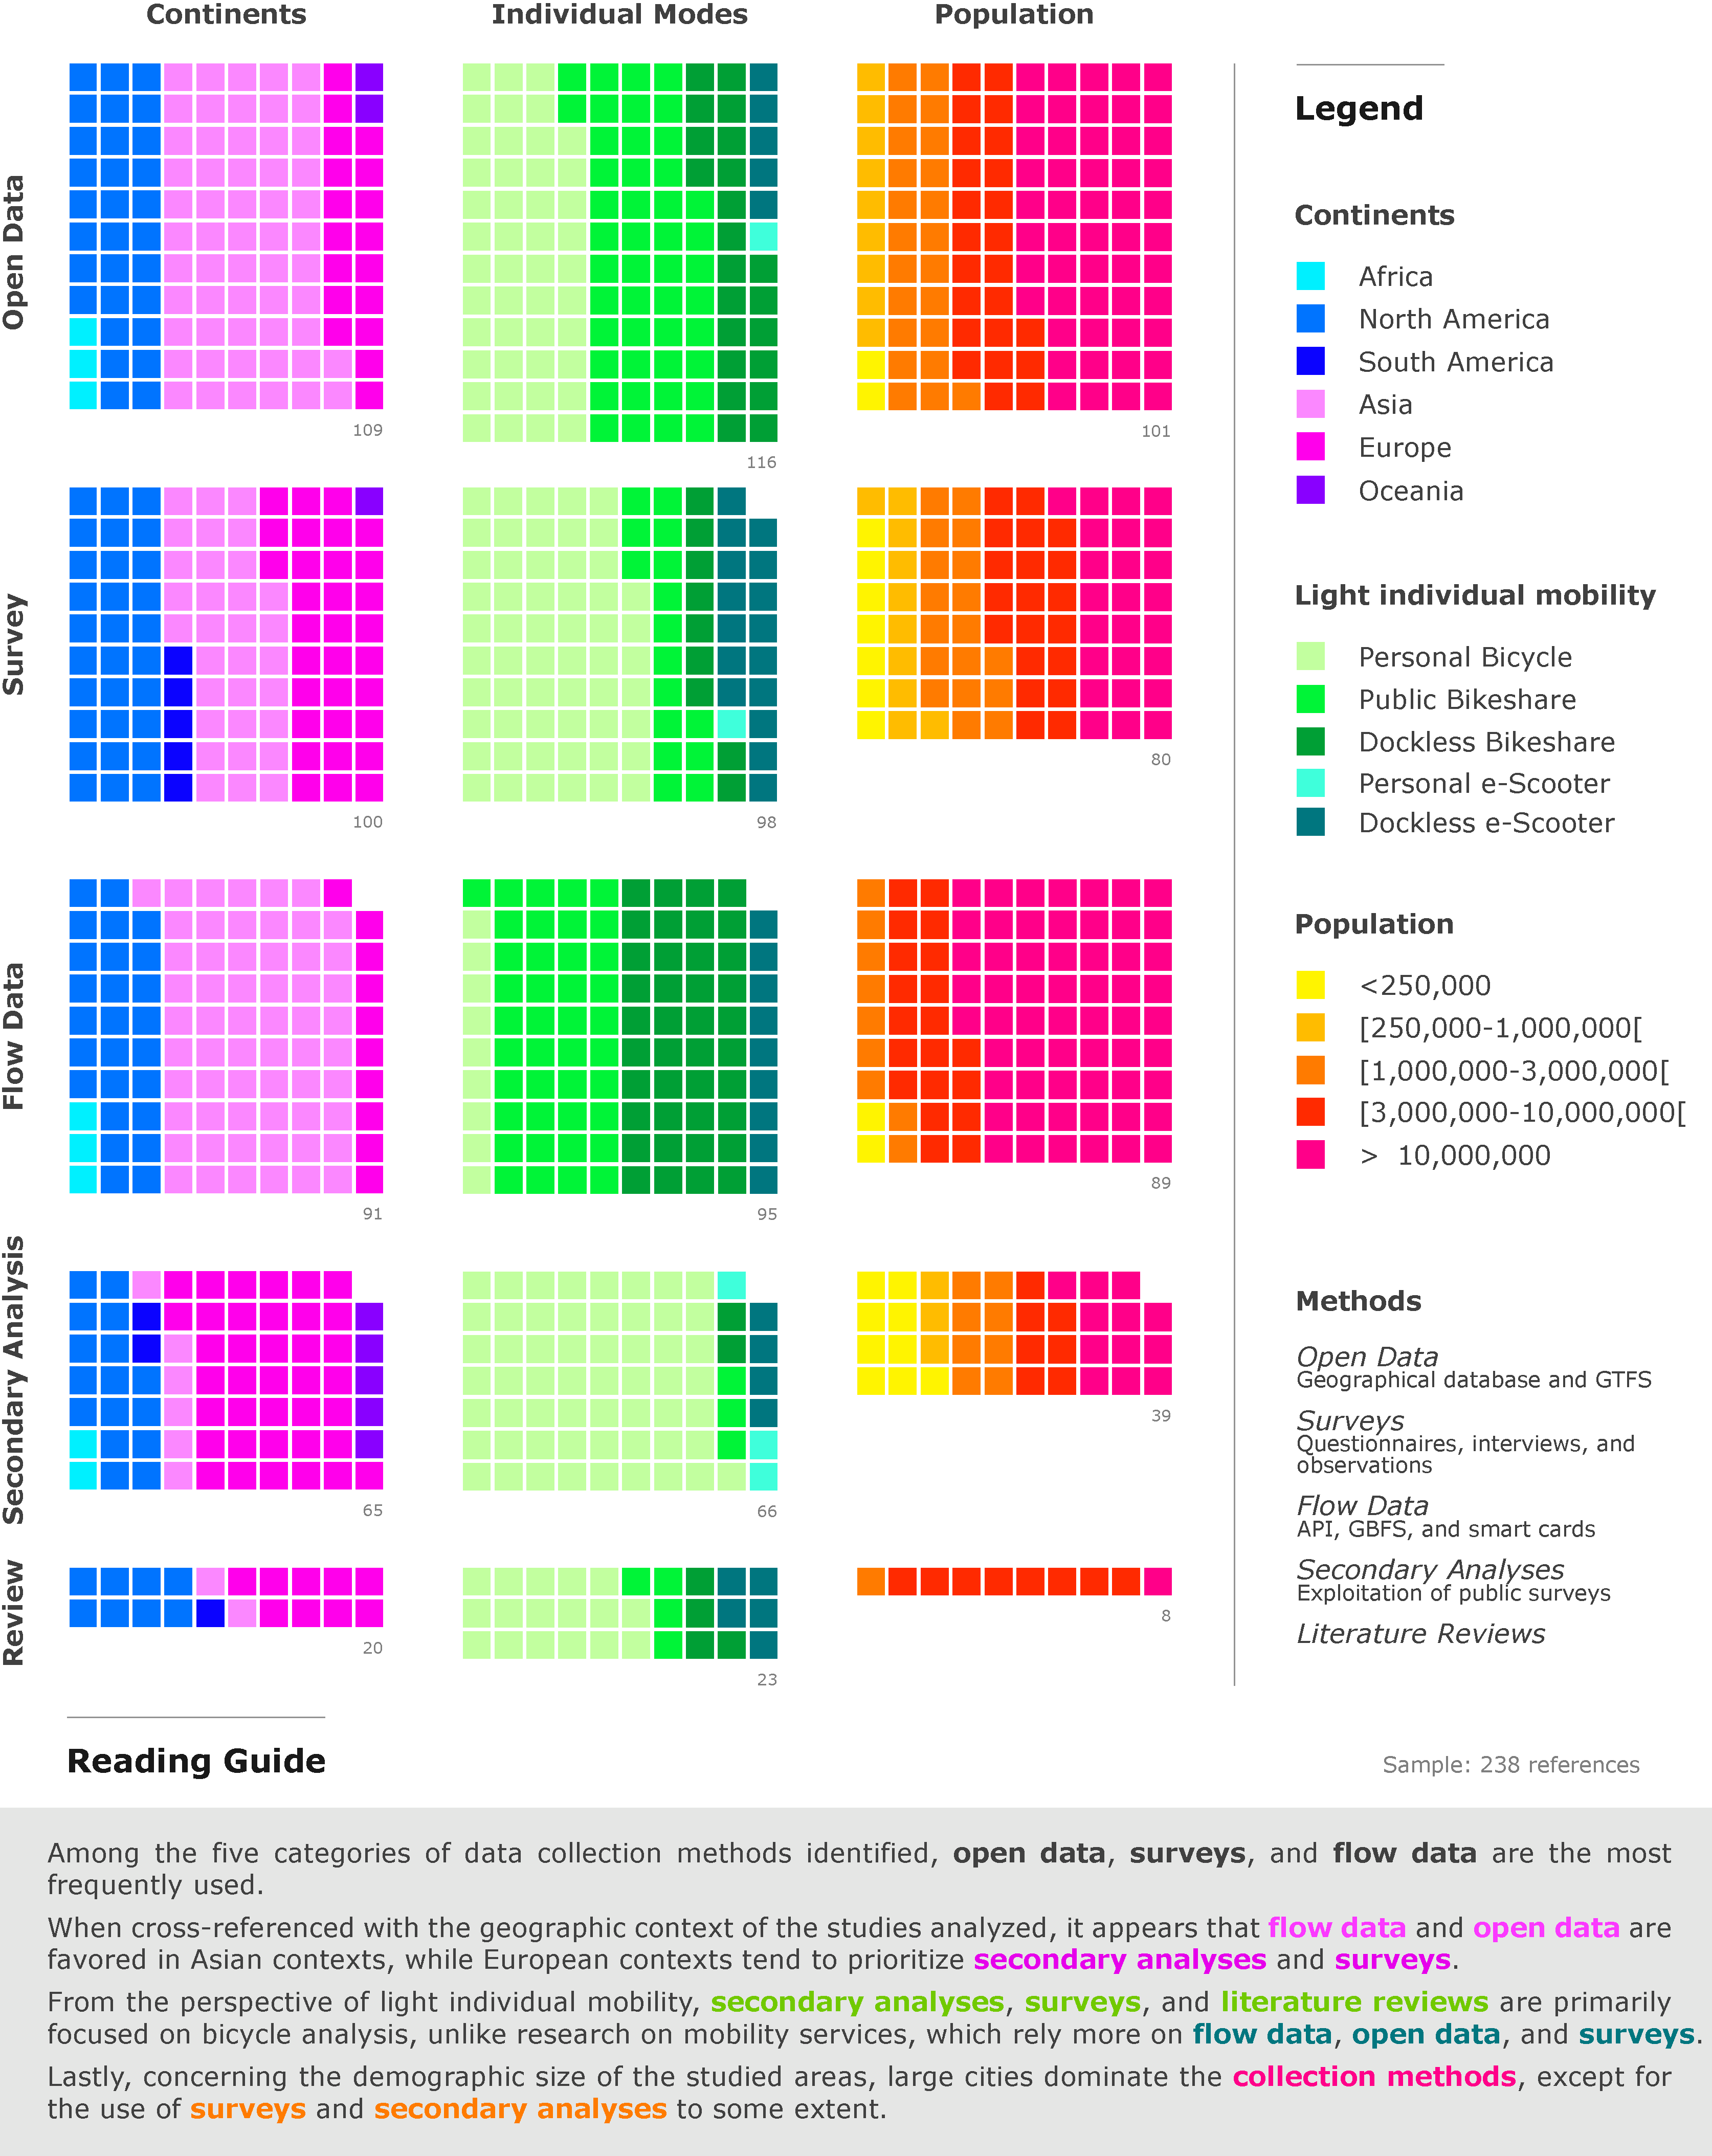
\includegraphics[width=1\columnwidth]{src/Figures/Chap-2/EN_RSL_Sources_donnees.pdf}}
    \vspace{5pt}
    \begin{flushright}\scriptsize{
    Author: \textcolor{blue}{Dylan Moinse (2023)}
    %\\
    %Created with \Marque{Excel}~and \Marque{Illustrator}
    }\end{flushright}
\end{figure}

% Data sources by urban agglomeration size
In a broader perspective, this methodological exploration reveals how urban size can influence distinct modes of investigation regarding empirical access to the field and information. By examining the typology of intermunicipalities, it becomes possible to identify patterns that suggest certain strategies for exploiting available data on the study areas. Thus, \hyperref[fig-chap2:sources-donnees-rsl]{Figure~\ref{fig-chap2:sources-donnees-rsl}} (page~\pageref{fig-chap2:sources-donnees-rsl}) highlights an overrepresentation of megacities within \textsl{Big Data}, with particular emphasis on \acrshort{API} and \acrshort{GBFS}. This predominance results from the concentration of bicycle and shared micromobility services, whether equipped with parking infrastructures or operating without them. In contrast, the data available regarding land use and public transport networks are more evenly distributed. Regarding the implementation of surveys through questionnaires, it is noteworthy that cities with fewer than three million inhabitants make greater use of online questionnaires. Agglomerations of at least 250,000 inhabitants tend to favor face-to-face questionnaires. Furthermore, secondary analysis of public surveys proves to be a preferred option in a significant proportion of smaller demographic agglomerations. This statistical interpretation can be explained by the differences in resource availability according to the specificities of the geographical areas. Indeed, massive data on a given territory are more rarely compiled in sparsely populated areas, and surveys help address this situation while being more accessible and less time-consuming.%%Translated%%

% Data sources by micromobility
The analysis of data collection methods has been cross-referenced with the forms of light individual mobility as they are addressed in the scientific corpus. While personal and intermodal bicycle use is primarily studied through face-to-face questionnaires or secondary analysis, the study of shared bicycles and micromobility relies heavily on the use of \textsl{Big Data}. On one hand, the examination of the \acrshort{PBS} system largely revolves around data generated by \acrshort{GBFS}. On the other hand, the investigation of \acrshort{DBS} and \acrshort{DESS} services is primarily based on the exploitation of \acrshort{API} (see \hyperref[fig-chap2:sources-donnees-rsl]{Figure~\ref{fig-chap2:sources-donnees-rsl}}, page~\pageref{fig-chap2:sources-donnees-rsl}). Unlike light shared mobility, which generates a large amount of real-time data, data on personal bicycles is more difficult to access in the form of massive data. Research on this mode of individual transport seems to focus on pre-existing surveys or field surveys in direct interaction with users.%%Translated%%

% Data sources examples face-to-face questionnaire
As an example, we can cite research on personal bicycle use and the use of face-to-face questionnaires by \textcolor{blue}{\textcite[1696]{cheng_evaluating_2012}}\index{Cheng, Yung-Hsiang|pagebf}\index{Liu, Kuo-Chu|pagebf} in association with the subway in Kaohsiung (386 responses), by \textcolor{blue}{\textcite[41]{jansson_almeida_alternativas_2022}}\index{Jansson Almeida, Bárbara|pagebf} with the subway in Porto Alegre (212 responses), by \textcolor{blue}{\textcite[183]{pan_intermodal_2010}}\index{Pan, Haixiao|pagebf}\index{Shen, Qing|pagebf}\index{Xue, Song|pagebf} on bicycles and \acrfull{e-Bike} with the subway in Shanghai (600 responses), by \textcolor{blue}{\textcite[7]{bauer_influence_2021}}\index{Bauer, Marek|pagebf}\index{Kisielewski, Piotr|pagebf} with the train and bus in Tarnow (501 responses), by \textcolor{blue}{\textcite[685, 4]{rastogi_travel_2003, rastogi_willingness_2010}}\index{Rastogi, Rajat|pagebf}\index{Krishna Rao,~K.~V.|pagebf} on walking and cycling with the train in Mumbai (1,449 responses), by \textcolor{blue}{\textcite[2]{rijsman_walking_2019}}\index{Rijsman, Lotte|pagebf}\index{Oort, Niels van|pagebf}\index{Ton, Danique|pagebf}\index{Hoogendoorn, Serge|pagebf}\index{Molin, Eric|pagebf}\index{Teijl, Thomas|pagebf} on walking and cycling with the tram in The Hague (629 responses), or by \textcolor{blue}{\textcite[192]{sherwin_practices_2011}}\index{Sherwin, Henrietta|pagebf}\index{Parkhurst, Graham|pagebf}\index{Robbins, Derek|pagebf}\index{Walker, Ian|pagebf} who combine the questionnaire and direct observation on bicycles with the train in Bristol (135 responses).%%Translated%%

% Data sources examples online questionnaire
Studies conducted using online questionnaires also show an imbalanced distribution in favor of personal bicycle use, as seen in the publications of \textcolor{blue}{\textcite[724]{waerden_relation_2018}}\index{Waerden, Peter|pagebf}\index{Waerden, Jaap|pagebf} on the combination of bicycles with trains in Eindhoven (415 responses), \textcolor{blue}{\textcite[5, 488]{la_paix_puello_train_2016, la_paix_puello_role_2021}}\index{La Paix Puello, Lissy|pagebf}\index{Geurs, Karst~T.|pagebf} with trains in the Rotterdam-The Hague metropolitan area and Randstad South (1,524 responses), \textcolor{blue}{\textcite[267]{krygsman_multimodal_2004}}\index{Krygsman, Stephan|pagebf}\index{Dijst, Martin|pagebf}\index{Arentze, Theo|pagebf} on bicycles with trains, subways, trams, and buses in the Amsterdam-Utrecht metropolitan area (1,966 households, including 755 cyclists), \textcolor{blue}{\textcite[663]{mil_insights_2020}}\index{Mil, Joeri~F.P. van|pagebf}\index{Leferink, Tessa~S.|pagebf}\index{Annema, Jan Anne|pagebf}\index{Oort, Niels van|pagebf} with trains in the Netherlands (269 responses), \textcolor{blue}{\textcite[132-133]{chen_determinants_2012}}\index{Chen, Lijun|pagebf}\index{Pel, Adam~J.|pagebf}\index{Chen, Xuewu|pagebf}\index{Sparing, Daniel|pagebf}\index{Hansen, Ingo~A.|pagebf} with the subway in Nanjing (1,784 responses, including 136 intermodal cyclists), \textcolor{blue}{\textcite[4259]{bopp_examining_2015}}\index{Bopp, Melissa|pagebf}\index{Gayah, Vikash~V.|pagebf}\index{Campbell, Matthew~E.|pagebf} on walking and cycling with trains, subways, and trams in Delaware, New Jersey, Maryland, West Virginia, Pennsylvania, and Ohio (1,234 responses, including 152 travelers), \textcolor{blue}{\textcite[6]{jonkeren_bicycle-train_2021, jonkeren_bicycle_2021}}\index{Jonkeren, Olaf|pagebf}\index{Kager, Roland|pagebf}\index{Harms, Lucas|pagebf}\index{te Brömmelstroet, Marco|pagebf} on bicycle use and parking in Rotterdam, Utrecht, Eindhoven, and around Dutch train stations (2,299 and 1,209 responses, including 1,309 intermodal cyclists), or \textcolor{blue}{\textcite[6]{molin_bicycle_2015}}\index{Molin, Eric|pagebf}\index{Maat, Kees|pagebf} on bicycle parking around Delft train station (866 responses).%%Translated%%

% Data sources examples secondary analysis
The dichotomy between data collection methods for these personal and shared modes of transport is also visible in the scientific work of \textcolor{blue}{\textcite[87]{taylor_analysis_1996}}\index{Taylor, Dean|pagebf}\index{Mahmassani, Hani|pagebf} who conducted a mail survey to assess bicycle use in combination with buses in Texas (814 responses), \textcolor{blue}{\textcite[10]{pages_nouveaux_2021}}\index{Pages, Thibaud|pagebf}\index{Lammoglia, Adrien|pagebf}\index{Josselin, Didier|pagebf} who conducted an online questionnaire (280 responses) combined with interviews on intermodal electric scooter use, or \textcolor{blue}{\textcite[60]{rabaud_quand_2022}}\index{Rabaud, Mathieu|pagebf}\index{Richer, Cyprien|pagebf} who utilized more than 40 mobility surveys from 2015-2019 to study this \acrfull{ePMD} in intermodality in France (364 electric scooter users). In this regard, the reuse of primary data from public surveys highlights the significant presence of bicycles and, more broadly, light individual mobility, as shown in studies by \textcolor{blue}{\textcite[8-10]{shelat_analysing_2018}}\index{Shelat, Sanmay|pagebf}\index{Huisman, Raymond|pagebf}\index{Oort, Niels van|pagebf} on bicycles with trains in the Netherlands, using the national mobility survey \acrfull{OViN} from 2010-2015 (approximately 250,000 households, including 3,376 cyclists), by \textcolor{blue}{\textcite[9]{luan_better_2020}}\index{Luan, Xin|pagebf}\index{Cheng, Lin|pagebf}\index{Song, Yan|pagebf}\index{Zhao, Jinbao|pagebf} on bicycles with the subway, using the national mobility survey from Nanjing in 2014 (10,385 households, including 3,999 cyclists), by \textcolor{blue}{\textcite[3]{zuo_determining_2018}}\index{Zuo, Ting|pagebf}\index{Wei, Hang|pagebf}\index{Rohne, Andrew|pagebf} on bicycles with buses in Cincinnati, using the Ohio mobility survey from 2009-2010 (2,059 households), or by \textcolor{blue}{\textcite[76]{oostendorp_combining_2018}}\index{Oostendorp, Rebekka|pagebf}\index{Gebhardt, Laura|pagebf} on bicycles with trains, subways, trams, and buses in Berlin, using the Berlin population census (1,098 individuals, including 363 intermodal cyclists).%%Translated%%

% 2.2.2.3. Types of analysis
\needspace{1\baselineskip} % Reserve space
\subsubsection*{Approaches and Types of Analysis
    \label{chap2:demarches-types-analyses}
    }

% Introduction
As part of this doctoral research, a comprehensive analysis of the methods employed in the \acrshort{SLR} corpus was conducted, revealing a substantial diversity of categorized analysis techniques. In total, 484 analysis methods were identified, corresponding to 273 distinct approaches. Among these approaches, modeling stands out as the most frequently used analytical tool, with 62 occurrences within the corpus. It is closely followed by the use of \acrfull{GIS}, which was recorded 51 times. Questionnaires are also frequently used, with 30 mentions. Finally, literature reviews, cited 17 times, highlight the importance of synthesizing existing knowledge. The diversity of techniques revealed reflects a broad range of approaches, from quantitative to qualitative. This methodological variety allows the study of urban mobility issues from multiple perspectives, providing a richer and more nuanced understanding of the interactions between light individual mobility integrated into public transport systems and urban systems.%%Translated%%

% Descriptive statistics (quantitative)
In relation to the research topic on \acrshort{M-TOD}, the quantitative approach is the most commonly used analysis method, with a marked presence of descriptive measures in 80 scientific articles and modeling in 62 studies. On one hand, descriptive statistical analysis is noted in 50 publications, followed by questionnaires based on stated preferences (\textsl{Stated Preference}, SP)\footnote{~
    Stated preference questionnaires are a data collection technique where respondents are asked about their preferences in hypothetical scenarios, in order to estimate the value attributed to goods, services, or changes in usage.
} and revealed preferences (\textsl{Revealed Preference}, RP)\footnote{~
    Revealed preference questionnaires are a data collection technique based on observing individuals' choices in real-world conditions.
} in 20 and 10 articles, respectively. On the other hand, studies that involve statistical modeling embrace a diversity of approaches. Nine studies use demand forecasting models (\textsl{Demand Forecasting Models}, DFM)\footnote{~
    A demand forecasting model is an econometric tool used to estimate the future demand for a product or service, depending on multiple variables such as price, income, or consumer preferences.
}, fifteen use discrete choice models (\textsl{Discrete Choice Models}, DCM)\footnote{~
    A discrete choice model is an econometric tool used to predict choices made by individuals from a finite set of options, based on random utility theory, where an individual's choice is modeled as a function of various attributes of the available options.
}, with seven applying the multinomial logit model (\textsl{Multinomial Logit Model}, MLN)\footnote{~
    The multinomial logit model is an extension of the binary logit model, used to model choices among more than two discrete alternatives, typically modes of transportation.
}, while another seven rely on ordinary least squares regression (\textsl{Ordinary Least Squares Regression}, OLS)\footnote{~
    Ordinary least squares regression is a linear regression method that minimizes the sum of the squared differences between observed values and those estimated by the model.
}. These frequently used regression models provide a robust approach for analyzing relationships between variables. Additionally, some studies adopt a clustering approach, notably k-means clustering (\textsl{k-means clustering})\footnote{~
    K-means is a clustering method designed to divide a dataset into $k$ distinct groups, while minimizing the variance within the cluster and maximizing the variance between the classes.
}, present in seven articles. Finally, \acrfull{CBEA})\footnote{~
    Cost-benefit analysis is used to assess the expected benefits and associated costs of a project in order to determine its viability and the best options.
} is present in three publications, while traffic models are mentioned in two studies.%%Translated%%

% Cartography (GIS)
The application of methods related to quantitative data science (\textsl{Data Science}) is also manifested through the geostatistical approach. This relies particularly on the use of \acrshort{GIS}, a spatial analysis tool integrated into 51 documents studied within the corpus. Alongside the direct use of \acrshort{GIS}, various complementary spatial analysis techniques are implemented. Among these methods, geographically weighted regression (\textsl{Geographically Weighted Regression}, GWR)\footnote{~
    Geographically weighted regression is a spatial modeling technique that analyzes spatial variation in relationships between variables by assigning a different weight to each observation based on its location.
}, used in nine studies, stands out. Eight studies incorporate spatial autocorrelation\footnote{~
    Spatial autocorrelation is measured using Moran's index, for example. This index is used in geostatistics to assess whether a model exhibits random, clustered, or dispersed spatial patterns. A Moran index close to +1 indicates a strong positive spatial correlation, while an index close to -1 indicates a strong negative spatial correlation.
}, while the measurement of the network connectivity index (\textsl{Network Connectivity Index}, NCI)\footnote{~
    The network connectivity index is a quantitative measure used to evaluate the degree of connectivity within a transport or communication network by considering the number of links, the directionality of connections, and the distance between each node.
}, is used in seven studies. Two studies distinguish themselves by determining the node-place index (\textsl{Node-Place Index})\footnote{~
    The node-place index is a spatial analysis tool used to evaluate the functionality of transport nodes in their urban context by combining transport and urban planning aspects to assess the interactions between public transport stations and the urban environment.
}. Finally, kernel density estimation is applied in one study, as well as the Voronoi diagram\footnote{~
    The Voronoi diagram is a partitioning of a specific set of points on a Euclidean plane into cells. Each point generates a cellular region containing all points in the plane that are closer to this point than to any other.
}. These diverse approaches demonstrate the richness and complexity of spatial analyses in the study of \acrshort{M-TOD}, which are then enriched by qualitative approaches.%%Translated%%

% Discourse (qualitative)
The qualitative methodological approach is confined to a corpus of eleven publications. Among these, nine are primarily based on discourse analysis, conducted using semi-structured interviews, while the other two stand out for their sensitive exploration of the urban environment and social interactions. However, the qualitative approach can also be extended to the seventeen literature reviews that indirectly synthesize the research topic related to \acrshort{M-TOD}. These methods come from a variety of knowledge fields, ranging from economics, with approaches such as econometrics (DCM and MLN) and transport economics (SP, RP, DFM, and transport models); to statistics, including data sciences and k-means. They also encompass geography, with spatial analysis (Voronoi diagram and GWR); and touch sociology, particularly through interviews.%%Translated%%

% ___________________________________________
% 2.3.
\newpage
\needspace{1\baselineskip} % Reserve space
\sectionheader{Current Knowledge on M-TOD}
\section{Characterization of a \textsl{Micromobility-friendly Transit-Oriented Development} through the Lens of Urban Environment Characteristics and Individual Choices
    \label{chap2:caracterisation-btod-environnement-urbain-choix-individuels}
    }

% Introduction 1
The current section of this chapter is dedicated to a detailed study aiming to define the fundamental attributes of \acrshort{M-TOD}, viewed through the lens of the urban environment and personal mobility preferences. To this end, we have chosen an inductive approach structured around the \Commas{\acrshort{7Ds}} enriched with additional variables related to the intermodal practices examined. The goal of this analysis derived from the \acrshort{SLR} is to outline the contours of the \acrshort{M-TOD} urban model, based on a perspective of international empirical studies. It aims to identify the recurring characteristics emerging from this literature review. Consequently, our ambition is also to understand how \acrshort{M-TOD} can be viewed as a complement to \acrshort{TOD} and to grasp how the analyzed dimensions of this urban concept are reflected in an urban strategy that integrates light individual mobility.%%Translated%%

% Introduction 2
Through their \acrshort{SLR}, \textcolor{blue}{\textcite[294]{zhang_built_2023}}\index{Zhang, Yushan|pagebf}\index{Kasraian, Dena|pagebf}\index{Wesemael, Pieter van|pagebf} reveal how studies focusing on bicycles and micromobility specifically concentrate on management and operational strategies for these modes of transport, as well as on the analysis of user profiles and behaviors. However, less attention has been paid to the interrelation between light individual mobility and the urban environment. Therefore, this chapter mainly focuses on exploring this essential yet under-examined aspect, which is crucial in the conceptualization of \acrshort{M-TOD}. According to the definition established by \textcolor{blue}{\textcite[65]{handy_how_2002}}\index{Handy, Susan~L.|pagebf}\index{Boarnet, Marlon~G.|pagebf}\index{Ewing, Reid|pagebf}\index{Killingsworth, Richard~E.|pagebf}, the urban environment is distinguished by three major components: (i) urban design, encompassing the configuration of public spaces; (ii) land use, relating to the location, distribution, and density of activities in space; and (iii) the mobility system, which includes both transport infrastructure and the level of service of networks (\textsl{Level of Service}, LoS). It is based on these conceptual foundations that our data analysis is built, resulting in a summary table where each study has been evaluated based on the presence or absence of these dimensions (see \hyperref[annexes:rsl-resultats]{Appendix~\ref{annexes:rsl-resultats}}, page~\pageref{annexes:rsl-resultats}).%%Translated%%

% Plan announcement
This section will then attempt to characterize \acrshort{M-TOD}, with the aim of presenting a definition of this urban model based on the knowledge derived from scientific literature. Various aspects will be addressed, starting with the \Commas{\acrshort{7Ds}}, namely \hyperref[chap2:densite-population]{population density (\(D1\))} (page~\pageref{chap2:densite-population}), \hyperref[chap2:diversite-fonctionnelle]{functional land-use diversity (\(D2\))} (page~\pageref{chap2:diversite-fonctionnelle}), \hyperref[chap2:traitement-espaces-publics]{design of public spaces (\(D3\))} (page~\pageref{chap2:traitement-espaces-publics}), \hyperref[chap2:accessibilite-intermodale]{accessibility to territorial resources (\(D4\))} (page~\pageref{chap2:accessibilite-intermodale}), \hyperref[chap2:distances-premiers-derniers-km]{station-area size (\(D5\))} (page~\pageref{chap2:distances-premiers-derniers-km}), \hyperref[chap2:gestion-demande-mobilite]{mobility demand management (\(D6\))} (page~\pageref{chap2:gestion-demande-mobilite}), \hyperref[chap2:sociodemographie-usagers]{dimension of social inclusion (\(D7\))} (page~\pageref{chap2:sociodemographie-usagers}), followed by \hyperref[chap2:comportements-mobilite]{mobility behaviors} (page~\pageref{chap2:comportements-mobilite}) and \hyperref[chap2:impacts-systemes-urbain-mobilite]{various impacts} (page~\pageref{chap2:impacts-systemes-urbain-mobilite}).%%Translated%%

% 2.3.1. Results: Density
\needspace{1\baselineskip} % Reserve space
\subsection{Population Density
    \label{chap2:densite-population}
    }

% Introduction
The first topic addressed in this section is population density, a crucial element for \acrshort{TOD}, supporting the development of compact areas that are favorable to pedestrians. Present in 44 of the 238 scientific publications examined, demographic density positively influences the combined use of public transport and light individual mobility.%%Translated%%

% 2.3.1.1. Positive Impact of Population Density
\needspace{1\baselineskip} % Reserve space
\subsubsection*{Positive Association with Population Density
    \label{chap2:association-positive-densite-population}
    }

% Positive impact of population density with personal bicycle
Within the body of studies examined, a significant proportion of works suggest the existence of a positive correlation between population density and the interaction between public transport systems and light individual mobility. These academic studies highlight that areas characterized by higher population density tend to experience more intensive use of bicycles and micromobility, in complementarity with public transport networks. In this context, population density proves to be a predominant dimension, with a positive relationship established between this factor and the likelihood of using a bicycle in combination with trains and buses in Denmark \textcolor{blue}{\autocite[41]{nielsen_bikeability_2018}}\index{Nielsen, Thomas Alexander Sick|pagebf}\index{Skov-Petersen, Hans|pagebf}. Similarly, in the United States, the modal share of bicycles combined with trains and buses has notably increased in high-density areas \textcolor{blue}{\autocite[107]{wang_bicycle-transit_2013}}\index{Wang, Rui|pagebf}\index{Liu, Chen|pagebf}. \textcolor{blue}{\textcite[212]{kager_characterisation_2016}}\index{Kager, Roland|pagebf}\index{Bertolini, Luca|pagebf}\index{te Brömmelstroet, Marco|pagebf} assert that bicycles effectively complement trains in dense environments, but also adapt to lower densities in various contexts, notably in Amsterdam, Amstelveen, Diemen, and Ouder-Amstel. In Amsterdam, \textcolor{blue}{\textcite[344]{kampen_bicycle_2021}}\index{Kampen, Jullian van|pagebf}\index{Pauwels, Eric|pagebf}\index{Mei, Rob van der|pagebf}\index{Dugundji, Elenna~R.|pagebf} found that building density plays a crucial role in the choice of personal bicycle parking locations, with high-density urban neighborhoods attracting more bike parking near train stations and metro stations.%%Translated%%

% Positive impact of population density with bike-sharing
In a similar perspective regarding bike-sharing, a positive link is suggested between population density and the use of \acrshort{PBS} in synergy with the railway network, as observed in Chicago, New York City, and Washington D.C. \textcolor{blue}{\autocite[16]{kong_deciphering_2020}}\index{Kong, Hui|pagebf}\index{Jin, Scarlett~T.|pagebf}\index{Sui, Daniel~Z.|pagebf}. This interrelation is also confirmed between \acrshort{PBS} and the subway, both in Beijing \textcolor{blue}{\autocite[9]{yu_understanding_2021}}\index{Yu, Senbin|pagebf}\index{Liu, Gehui|pagebf}\index{Yin, Congru|pagebf} and Nanjing \textcolor{blue}{\autocite[12]{chen_what_2022}}\index{Chen, Wendong|pagebf}\index{Chen, Xuewu|pagebf}\index{Chen, Jingxu|pagebf}\index{Cheng, Long|pagebf}. \textcolor{blue}{\textcite[15]{li_investigating_2022}}\index{Li, Xiaofeng|pagebf}\index{Wu, Yao-Jan|pagebf}\index{Khani, Alireza|pagebf} suggest that in high-density areas, a positive interaction is observed between \acrshort{PBS} and trams and buses, in Tucson. In Oslo, \textcolor{blue}{\textcite[399]{bocker_bike_2020}}\index{Böcker, Lars|pagebf}\index{Anderson, Ellinor|pagebf}\index{Uteng, Tanu Priya|pagebf}\index{Throndsen, Torstein|pagebf} emphasize that the frequent use of \acrshort{PBS} in combination with the subway is predominant in densely populated areas.%%Translated%%

% Positive impact of population density with electric shared bikes
Several studies conducted in Shenzhen and Shanghai, respectively by \textcolor{blue}{\textcite[6]{wang_relationship_2020}}\index{Wang, Ruoyu|pagebf}\index{Lu, Yi|pagebf}\index{Wu, Xueying|pagebf}\index{Liu, Ye|pagebf}\index{Yao, Yao|pagebf} and \textcolor{blue}{\textcite[31]{lin_analysis_2019}}\index{Lin, Diao|pagebf}\index{Zhang, Yongping|pagebf}\index{Zhu, Ruoxin|pagebf}\index{Meng, Liqiu|pagebf}, corroborate that high population densities are positively associated with the use of \acrshort{DBS} with the subway, revealing an increased demand in dense urban areas. \textcolor{blue}{\textcite[16]{li_operating_2019}}\index{Li, Yuan|pagebf}\index{Zhu, Zhenjun|pagebf}\index{Guo, Xiucheng|pagebf} highlighted, through a classification of subway stations, that those located in densely populated urban neighborhoods of Nanjing experience higher \acrshort{DBS} usage for the \Commas{first and last miles.} The work of \textcolor{blue}{\textcite[25]{guo_dockless_2021}}\index{Guo, Yuanyuan|pagebf}\index{Yang, Linchuan|pagebf}\index{Lu, Yi|pagebf}\index{Zhao, Rui|pagebf} and \textcolor{blue}{\textcite[184]{cheng_exploring_2022}}\index{Cheng, Long|pagebf}\index{Wang, Kailai|pagebf}\index{Vos, Jonas de|pagebf}\index{Huang, Jie|pagebf}\index{Witlox, Frank|pagebf} show that population density is significantly related to integrated use of \acrshort{DBS} with the subway during peak hours, respectively in Shenzhen and Nanjing. In Suzhou, \textcolor{blue}{\textcite[24]{li_integration_2020}}\index{Li, Jie|pagebf}\index{Lu, Yang|pagebf}\index{Ling, Lei|pagebf} observe that higher population density reduces the likelihood of choosing the bus in favor of \acrshort{DBS} to reach subway stations. In Beijing, \textcolor{blue}{\textcite[11]{liu_temporal_2022}}\index{Liu, Siyang|pagebf}\index{Zhang, Xiaodong|pagebf}\index{Zhou, Chenjing|pagebf}\index{Rong, Jian|pagebf}\index{Bian, Yang|pagebf} reveal that a 10\% increase in density leads to a significant rise in \acrshort{DBS} use with the subway on weekdays, and even more so during morning peak hours. A similar conclusion emerges for \acrshort{DESS} with the subway, where a concentration has been identified in densely populated areas of New York City \textcolor{blue}{\autocite[16]{lee_forecasting_2021}}\index{Lee, Mina|pagebf}\index{Chow, Joseph|pagebf}\index{Yoon, Gyugeun|pagebf}\index{He, Brian|pagebf}.%%Translated%%

% Positive impact of population density with public transport
The analysis of the \acrshort{SLR} also tends to highlight an increase in the use of public transport, questioning the links between demographic density and the intermodal use of light individual mobility. High-density areas thus promote the use of public transport by attracting a growing number of passengers who adopt bicycles and micromobility. In the residential neighborhoods of the Netherlands, population density proves to be a key factor that significantly influences public transport use, including trains, subways, trams, buses, and even ferries, by cyclists \textcolor{blue}{\autocite[334]{martens_promoting_2007}}\index{Martens, Karel|pagebf}. In Shanghai, research conducted by \textcolor{blue}{\textcite[10]{li_exploring_2021}}\index{Li, Wenxiang|pagebf}\index{Chen, Shawen|pagebf}\index{Dong, Jieshuang|pagebf}\index{Wu, Jingxian|pagebf} indicates that population density is positively correlated with transfer distance, both in \gls{access} and \gls{egress}, suggesting that subway stations attract \acrshort{DBS} users from further distances. Furthermore, during the post-access phase from subway stations, population density in Kaohsiung significantly stimulates passengers' intention to use \acrshort{PBS} \textcolor{blue}{\autocite[29]{cheng_expanding_2018}}\index{Cheng, Yung-Hsiang|pagebf}\index{Li, Yi-Chun|pagebf}.%%Translated%%

% 2.3.1.2. Complex Impact of Population Density
\needspace{1\baselineskip} % Reserve space
\subsubsection*{Complex Relations with Population Density
    \label{chap2:relations-complexes-densite-population}
    }

% Complex relationship between density and intermodality
The examination of the relationship between population density and the intermodal use of bicycles and micromobility reveals increased complexity within part of the studied corpus, with some research highlighting a more nuanced, even ambiguous, correlation between these different variables. Several studies suggest that population density is not a determining factor in the joint use of light individual mobility, particularly regarding bicycles and trains in Melbourne \textcolor{blue}{\autocite[403]{weliwitiya_bicycle_2019}}\index{Weliwitiya, Hesara|pagebf}\index{Rose, Geoff|pagebf}\index{Johnson, Marilyn|pagebf}, \acrshort{PBS} and buses in Birmingham \textcolor{blue}{\autocite[5]{glass_role_2020}}\index{Glass, Caroline|pagebf}\index{Appiah-Opoku, Seth|pagebf}\index{Weber, Joe|pagebf}\index{Jones, Steven~L.|pagebf}\index{Chan, Amber|pagebf}\index{Oppong, Judith|pagebf}, or \acrshort{DBS} and the subway in Shenzhen \textcolor{blue}{\autocites[11]{guo_built_2020}[388]{guo_role_2021}}\index{Guo, Yuanyuan|pagebf}\index{He, Sylvia~Y.|pagebf}. In Utrecht, \textcolor{blue}{\textcite[274]{krygsman_multimodal_2004}}\index{Krygsman, Stephan|pagebf}\index{Dijst, Martin|pagebf}\index{Arentze, Theo|pagebf} demonstrated a nonlinear relationship between population density and bicycle use, particularly around train stations and metro, tram, and bus stations, where higher urban density tends to favor shorter distances, conducive to walking. Higher population density in Beijing does not seem to have a notable effect on \acrshort{PBS} use, unlike an increased use of taxis, particularly by female users, to reach the subway \textcolor{blue}{\autocite[15]{ni_exploring_2020}}\index{Ni, Ying|pagebf}\index{Chen, Jiaqi|pagebf}. In Beijing, \acrshort{PBS} use in combination with the subway increases with population density, but this correlation is not observed in models applied to Taipei and Tokyo \textcolor{blue}{\autocite[216]{lin_built_2018}}\index{Lin, Jen-Jia|pagebf}\index{Zhao, Pengjun|pagebf}\index{Takada, Kazuyuki|pagebf}\index{Li, Shengxiao|pagebf}\index{Yai, Tetsuo|pagebf}\index{Chen, Chi-Hao|pagebf}. In a similar context, \textcolor{blue}{\textcite[45]{la_paix_puello_modelling_2015}}\index{La Paix Puello, Lissy|pagebf}\index{Geurs, Karst~T.|pagebf} noted that high density seems to discourage the use of bicycles to reach stations in the Randstad South area. Similarly, significant population density near subway stations in Nanjing seems to favor walking as the mode of access to the rail network, rather than \acrshort{PBS} \textcolor{blue}{\autocite[17]{ji_public_2017}}\index{Ji, Yanjie|pagebf}\index{Fan, Yingling|pagebf}\index{Ermagun, Alizera|pagebf}\index{Cao, Xuening|pagebf}\index{Wang, Wei|pagebf}\index{Das, Kirti|pagebf}. \textcolor{blue}{\textcite[181]{gan_associations_2021}}\index{Gan, Zuoxian|pagebf}\index{Yang, Min|pagebf}\index{Zeng, Qingcheng|pagebf}\index{Timmermans, Harry~J.~P.|pagebf} reveal that a 1\% increase in population density increases the likelihood of choosing walking by 0.22\% for access and 0.36\% for egress from a subway station in Nanjing. In a specific case study of the Mouans-Sartoux train station area, \textcolor{blue}{\textcite[189]{moinse_intermodal_2022}}\index{Moinse, Dylan|pagebf}\index{Goudeau, Matthieu|pagebf}\index{L'Hostis, Alain|pagebf}\index{Leysens, Thomas|pagebf} observed that \acrshort{PeS} travelers more frequently begin and end their intermodal trip in dense areas, unlike personal bicycle travelers.%%Translated%%

% Reasons
The inclination towards densifying territories can thus be explained by improved accessibility and increased demand for mobility due to population concentration. The positive correlation between demographic density and increased use of light individual mobility in coordination with public transport may also be attributed to the additional costs associated with car use in densely populated areas, making bicycles more attractive near train station neighborhoods, as highlighted by \textcolor{blue}{\textcite[751]{midenet_modal_2018}}\index{Midenet, Sophie|pagebf}\index{Côme, Etienne|pagebf}\index{Papon, Francis|pagebf} in the case of Amboise. \textcolor{blue}{\textcite[11]{hu_examining_2022}}\index{Hu, Songhua|pagebf}\index{Chen, Mingyang|pagebf}\index{Jiang, Yuan|pagebf}\index{Sun, Wei|pagebf}\index{Xiong, Chenfeng|pagebf} report that density is closely related to public transport supply in Shanghai: high-density areas near downtown exhibit fewer \acrshort{DBS} activities with the subway compared to peripheral urban areas. In the context of Nanjing, \textcolor{blue}{\textcite[9]{cheng_promoting_2022}}\index{Cheng, Long|pagebf}\index{Jin, Tanhua|pagebf}\index{Wang, Kailai|pagebf}\index{Lee, Yongsung|pagebf}\index{Witlox, Frank|pagebf} and \textcolor{blue}{\textcite[8]{cheng_comparison_2023}}\index{Cheng, Long|pagebf}\index{Huang, Jie|pagebf}\index{Jin, Tanhua|pagebf}\index{Chen, Wendong|pagebf}\index{Li, Aoyong|pagebf}\index{Witlox, Frank|pagebf} observe that \acrshort{DBS} combined with the subway is favored when population density is high, but this trend reverses when density reaches a threshold between 18,000 and 23,000 inhabitants/km², beyond which the effects become uncertain, likely due to urban congestion, pollution, and safety risks. \textcolor{blue}{\textcite[8]{zhou_spatially_2023}}\index{Zhou, Xiao|pagebf}\index{Dong, Quanhua|pagebf}\index{Huang, Zhou|pagebf}\index{Yin, Ganmin|pagebf}\index{Zhou, Guoqing|pagebf}\index{Liu, Yu|pagebf} come to a similar conclusion, highlighting a nonsignificant relationship between density and the combined use of \acrshort{DBS} with the subway and bus in Beijing, due to crowded streets and denser traffic in high-density areas. According to \textcolor{blue}{\textcite[3]{romm_differences_2022}}\index{Romm, Daniel|pagebf}\index{Verma, Priyanka|pagebf}\index{Karpinski, Elizabeth|pagebf}\index{Sanders, Tracy~L.|pagebf}\index{McKenzie, Grant|pagebf}, bicycles are more frequently used for the \Commas{first miles} in densely populated urban neighborhoods of Boston due to lower motor vehicle ownership among residents.%%Translated%%

% Conclusion on Density
The existing association between demographic density and the use of light individual mobility, in synergy with public transport systems, within the theoretical framework of \acrshort{M-TOD}, reveals a certain complexity. On one hand, a body of empirical research affirms a positive connection between these factors, corroborating the key role of density in the secondary area of \acrshort{TOD}. On the other hand, a deeper exploration of the scientific literature reveals a series of sometimes contradictory findings regarding the clear influence of population density. In light of this review of the scientific literature dedicated to the role of this territorial parameter in the architecture of \acrshort{TOD}, it seems appropriate to adopt a nuanced approach. Among other things, the reviewed documentation would emphasize a relationship that, while complex, is verified, between population density and the integration of bicycles and micromobility with public transport. However, this relationship is dependent on a range of factors related to the specific characteristics of each urban system.%%Translated%%

% 2.3.2. Results: Diversity
\needspace{1\baselineskip} % Reserve space
\subsection{Functional Diversity
    \label{chap2:diversite-fonctionnelle}
    }

% Introduction
Diversity holds a prominent place in the urban planning of \acrshort{M-TOD}, primarily manifested through job density, the multiplicity of urban functions, and socio-economic diversity. These aspects have been highlighted in 36 of the studies constituting the \acrshort{SLR} corpus. Special attention has been given to land-use diversity, considered a favorable lever for integrating light individual mobility into public transport networks and stimulating territorial activity. The importance of clustering and concentrating residential areas, commercial spaces, offices, and green areas in the same space is widely recognized. However, the issue of diversity in social groups, particularly through a varied and affordable housing offer, remains underrepresented in studies related to extended train station neighborhoods.%%Translated%%

% 2.3.2.1. Employment Density
\needspace{1\baselineskip} % Reserve space
\subsubsection*{Employment Density
    \label{chap2:densite-emplois}
    }

% Positive impact of employment density
According to the majority of the scientific studies analyzed, it appears that employment density in neighborhoods near train stations, particularly those serving activity centers, significantly supports the integration of light individual mobility with public transport systems. Regarding intermodal use of personal bicycles, \textcolor{blue}{\textcite[12]{zuo_promote_2020}}\index{Zuo, Ting|pagebf}\index{Wei, Heng|pagebf}\index{Chen, Na|pagebf} note that an increase in jobs near bus stops in Hamilton leads to higher bicycle usage. Similarly, \textcolor{blue}{\textcite[41]{nielsen_bikeability_2018}}\index{Nielsen, Thomas Alexander Sick|pagebf}\index{Skov-Petersen, Hans|pagebf} highlight that a concentration of retail jobs in Denmark is strongly correlated with combined bicycle use, when parked at the origin station, and trains. Employment density is also positively related to the use of \acrshort{PBS} in combination with the subway in Washington D.C. \textcolor{blue}{\autocite[7]{ma_bicycle_2015}}\index{Ma, Ting|pagebf}\index{Liu, Chao|pagebf}\index{Erdoğan, Sevgi|pagebf} and in Nanjing \textcolor{blue}{\autocite[5]{cheng_comparison_2023}}\index{Cheng, Long|pagebf}\index{Huang, Jie|pagebf}\index{Jin, Tanhua|pagebf}\index{Chen, Wendong|pagebf}\index{Li, Aoyong|pagebf}\index{Witlox, Frank|pagebf}. \textcolor{blue}{\textcite[397]{bocker_bike_2020}}\index{Böcker, Lars|pagebf}\index{Anderson, Ellinor|pagebf}\index{Uteng, Tanu Priya|pagebf}\index{Throndsen, Torstein|pagebf} highlight that the access phase involving \acrshort{PBS} is closely associated with employment density around subway stations in Oslo. In Nanjing, \textcolor{blue}{\textcite[8]{cheng_promoting_2022}}\index{Cheng, Long|pagebf}\index{Jin, Tanhua|pagebf}\index{Wang, Kailai|pagebf}\index{Lee, Yongsung|pagebf}\index{Witlox, Frank|pagebf} observe that areas with high employment density, up to a threshold of 13,000 inhabitants/km², encourage the use of \acrshort{PBS} in combination with the subway. Finally, regarding \acrshort{DBS}, \textcolor{blue}{\textcite[181]{cheng_exploring_2022}}\index{Cheng, Long|pagebf}\index{Wang, Kailai|pagebf}\index{Vos, Jonas de|pagebf}\index{Huang, Jie|pagebf}\index{Witlox, Frank|pagebf} note that employment density around subway stations is positively associated with its evening use, but this association is not observed for morning trips.%%Translated%%

% Negative impact of employment density
However, it is worth noting that two studies stand out by challenging the generally accepted conclusions regarding the crucial role of employment density in train station neighborhoods. \textcolor{blue}{\textcite[10]{guo_built_2020}}\index{Guo, Yuanyuan|pagebf}\index{He, Sylvia~Y.|pagebf} and \textcolor{blue}{\textcite[389]{guo_role_2021}}\index{Guo, Yuanyuan|pagebf}\index{He, Sylvia~Y.|pagebf} highlighted a negative correlation between the concentration of jobs along subway lines and the use of \acrshort{DBS} during morning hours in Shenzhen. In a more nuanced approach, \textcolor{blue}{\textcite[214]{lin_built_2018}}\index{Lin, Jen-Jia|pagebf}\index{Zhao, Pengjun|pagebf}\index{Takada, Kazuyuki|pagebf}\index{Li, Shengxiao|pagebf}\index{Yai, Tetsuo|pagebf}\index{Chen, Chi-Hao|pagebf} developed a model indicating a positive relationship between employment density and the intermodal practice of subway with \acrshort{PBS} in Beijing, but contrasting with two other models in Taipei and Tokyo, where no such association was found.%%Translated%%

% 2.3.2.2. Functional Mix
\needspace{1\baselineskip} % Reserve space
\subsubsection*{Land Use
    \label{chap2:occupation-sols}
    }

% Positive impact of functional mix on integrated personal bicycle use
The examination of jobs located around public transport stops, particularly train stations at the \Commas{activity} end of trips, involves considering land use and primarily the diversity of functions in the studied areas. In this regard, a significant proportion of research highlights the role of urban mix as a founding principle for \acrshort{M-TOD}. Land-use diversity is positively linked to the likelihood of choosing walking and cycling to and from the subway in Nanjing: a 1\% increase in functional mix increases the probability of choosing these two modes of transport by 0.74\% and 0.75\%, respectively \textcolor{blue}{\autocite[182]{gan_associations_2021}}\index{Gan, Zuoxian|pagebf}\index{Yang, Min|pagebf}\index{Zeng, Qingcheng|pagebf}\index{Timmermans, Harry~J.~P.|pagebf}. Similarly, when the urban mix index increases by one unit, the number of cyclists going to train stations in Melbourne increases by 3.64 \textcolor{blue}{\autocite[401]{weliwitiya_bicycle_2019}}\index{Weliwitiya, Hesara|pagebf}\index{Rose, Geoff|pagebf}\index{Johnson, Marilyn|pagebf}. Additionally, the presence of food services and commercial activities plays a key role in determining the location of personal bicycle parking around newly opened subway stations in Amsterdam \textcolor{blue}{\autocite[343]{kampen_bicycle_2021}}\index{Kampen, Jullian van|pagebf}\index{Pauwels, Eric|pagebf}\index{Mei, Rob van der|pagebf}\index{Dugundji, Elenna~R.|pagebf}.%%Translated%%

% Positive impact of functional mix on integrated \acrshort{PBS} and \acrshort{DBS}
A similar finding emerges regarding \acrshort{PBS}: greater diversity in land use around subway stations fosters its integration. This trend is confirmed in Oslo \textcolor{blue}{\autocite[395]{bocker_bike_2020}}\index{Böcker, Lars|pagebf}\index{Anderson, Ellinor|pagebf}\index{Uteng, Tanu Priya|pagebf}\index{Throndsen, Torstein|pagebf}, as well as in Minneapolis and Saint-Paul \textcolor{blue}{\autocite[8]{song_investigating_2020}}\index{Song, Ying|pagebf}\index{Huang, Yuchuan|pagebf}, and in Shanghai \textcolor{blue}{\autocite[10]{yu_policy_2021}}\index{Yu, Qing|pagebf}\index{Li, Weifeng|pagebf}\index{Yang, Dongyuan|pagebf}\index{Xie, Yingkun|pagebf}. A similar observation is reported around train stations, subway stations, tram and bus stops in Boston, Chicago, Washington D.C., and New York City, as highlighted by \textcolor{blue}{\textcite[16]{kong_deciphering_2020}}\index{Kong, Hui|pagebf}\index{Jin, Scarlett~T.|pagebf}\index{Sui, Daniel~Z.|pagebf}. The combined use of \acrshort{PBS} and the subway is also encouraged in urban areas with many \acrfull{POIs} related to leisure in Nanjing \textcolor{blue}{\autocite[15-17]{ji_exploring_2018}}\index{Ji, Yanjie|pagebf}\index{Ma, Xinwei|pagebf}\index{Yang, Mingyuan|pagebf}\index{Jin, Yuchuan|pagebf}\index{Gao, Liangpeng|pagebf}, to shopping in Chengdu \textcolor{blue}{\autocite[889]{bi_analysis_2021}}\index{Bi, Hui|pagebf}\index{Ye, Zhirui|pagebf}\index{Zhang, Yi|pagebf}, and to restaurants in Nanjing, mainly outside peak hours and on weekends \textcolor{blue}{\autocite[11-13]{chen_what_2022}}\index{Chen, Wendong|pagebf}\index{Chen, Xuewu|pagebf}\index{Chen, Jingxu|pagebf}\index{Cheng, Long|pagebf}. Additionally, mixed land use is positively associated with the integration of \acrshort{DBS} and the subway in Nanjing, according to \textcolor{blue}{\textcite[12]{liu_use_2020}}\index{Liu, Yang|pagebf}\index{Feng, Tao|pagebf}\index{Ji, Yanjie|pagebf}\index{Shi, Zhuangbin|pagebf}, and in Shenzhen, as demonstrated by \textcolor{blue}{\textcite[6]{wang_relationship_2020}}\index{Wang, Ruoyu|pagebf}\index{Lu, Yi|pagebf}\index{Wu, Xueying|pagebf}\index{Liu, Ye|pagebf}\index{Yao, Yao|pagebf}. The presence of residential and industrial zones on the urban periphery is also positively related to \acrshort{DBS} use with the subway in Shenzhen, particularly in the morning for egress and in the evening for egress \textcolor{blue}{\autocites[10]{guo_built_2020}[389]{guo_role_2021}}\index{Guo, Yuanyuan|pagebf}\index{He, Sylvia~Y.|pagebf}.%%Translated%%

% Ambiguous impact of functional mix on integrated bicycle use
However, functional mix does not always have significantly positive effects, as revealed by part of the scientific literature. Several studies suggest that certain types of land use do not necessarily favor the integration of bike-sharing. According to \textcolor{blue}{\textcite[56]{zhao_bicycle-metro_2017}}\index{Zhao, Pengjun|pagebf}\index{Li, Shengxiao|pagebf}, the presence of public parks in Beijing increases the likelihood of combining bicycles with the subway, but shopping centers seem to discourage this integration, both for bicycles and \acrshort{PBS}. \textcolor{blue}{\textcite[9]{kim_analysis_2021}}\index{Kim, Minjun|pagebf}\index{Cho, Gi-Hyoung|pagebf} observe that the presence of a \acrfull{CBD}, or business district, commercial areas, and campuses works against a greater use of \acrshort{PBS} combined with the subway and bus, although a positive correlation is noted with residential areas in Seoul. Additionally, the models developed by \textcolor{blue}{\textcite[214]{lin_built_2018}}\index{Lin, Jen-Jia|pagebf}\index{Zhao, Pengjun|pagebf}\index{Takada, Kazuyuki|pagebf}\index{Li, Shengxiao|pagebf}\index{Yai, Tetsuo|pagebf}\index{Chen, Chi-Hao|pagebf} in Beijing and Tokyo do not show a significant link between \acrshort{PBS}, the subway, and land-use diversity. \textcolor{blue}{\textcite[5]{zhou_spatially_2023}}\index{Zhou, Xiao|pagebf}\index{Dong, Quanhua|pagebf}\index{Huang, Zhou|pagebf}\index{Yin, Ganmin|pagebf}\index{Zhou, Guoqing|pagebf}\index{Liu, Yu|pagebf} highlight a positive association between the presence of universities and educational and cultural spaces and the use of \acrshort{DBS} with the subway in Beijing, but also a negative association with shopping and leisure centers, and particularly negative with residential accommodation services. In contrast, in Shenzhen, \textcolor{blue}{\textcite[17]{guo_dockless_2021}}\index{Guo, Yuanyuan|pagebf}\index{Yang, Linchuan|pagebf}\index{Lu, Yi|pagebf}\index{Zhao, Rui|pagebf} find that office spaces tend to reduce \acrshort{DBS} use in combination with the subway, although mixed land use, including commercial and leisure areas, is positively related to these intermodal practices. In Shanghai, \textcolor{blue}{\textcite[9]{hu_examining_2022}}\index{Hu, Songhua|pagebf}\index{Chen, Mingyang|pagebf}\index{Jiang, Yuan|pagebf}\index{Sun, Wei|pagebf}\index{Xiong, Chenfeng|pagebf} emphasize that it is agricultural areas that discourage this combination, while residential and commercial spaces as well as higher education institutions increase \acrshort{DBS} use in conjunction with the subway. Finally, \textcolor{blue}{\textcite[7]{liu_temporal_2022}}\index{Liu, Siyang|pagebf}\index{Zhang, Xiaodong|pagebf}\index{Zhou, Chenjing|pagebf}\index{Rong, Jian|pagebf}\index{Bian, Yang|pagebf} reveal that green spaces and industrial zones in Beijing discourage the use of \acrshort{DBS} and the subway due to security and management restrictions, while land-use diversity generally has a positive impact.%%Translated%%

% Negative impact of functional mix on integrated bicycle use
In the analysis of the selected scientific corpus, two studies stand out by establishing a negative correlation between functional mix and the use of bike-sharing in intermodal transport. \textcolor{blue}{\textcite[8]{cheng_promoting_2022}}\index{Cheng, Long|pagebf}\index{Jin, Tanhua|pagebf}\index{Wang, Kailai|pagebf}\index{Lee, Yongsung|pagebf}\index{Witlox, Frank|pagebf} reveal that an increased proportion of land use for commercial purposes seems to discourage the use of \acrshort{PBS}, while land-use diversity has a negative influence on the use of \acrshort{DBS} in combination with the subway in Nanjing \textcolor{blue}{\autocite[10]{cheng_comparison_2023}}\index{Cheng, Long|pagebf}\index{Huang, Jie|pagebf}\index{Jin, Tanhua|pagebf}\index{Chen, Wendong|pagebf}\index{Li, Aoyong|pagebf}\index{Witlox, Frank|pagebf}. According to the authors, the increased presence of commercial areas is generally accompanied by an increase in the availability of car parking, while promoting functional mix seems to reduce the need for intermodal trips to destinations far from subway stations \textcolor{blue}{\autocite[5]{cheng_comparison_2023}}\index{Cheng, Long|pagebf}\index{Huang, Jie|pagebf}\index{Jin, Tanhua|pagebf}\index{Chen, Wendong|pagebf}\index{Li, Aoyong|pagebf}\index{Witlox, Frank|pagebf}.%%Translated%%

% 2.3.2.3. Social Mix
\needspace{1\baselineskip} % Reserve space
\subsubsection*{Social Mix
    \label{chap2:mixite-sociale}
    }

% Impact of social mix
A final aspect, related to diversity, can be explored from the perspective of social mix within the territories. Only one study in the analyzed corpus addresses the variety of housing types in the context of \acrshort{M-TOD}. This research, conducted by \textcolor{blue}{\textcite[115]{wang_bicycle-transit_2013}}\index{Wang, Rui|pagebf}\index{Liu, Chen|pagebf}, highlights that trips combining bicycle use with train or bus are more frequent in communities characterized by a high proportion of rental housing in the United States.%%Translated%%

% Conclusion on Diversity
It is evident that employment density and functional mix play a crucial role in promoting intermodality involving the use of light individual mobility. The majority of the studies analyzed agree on the positive influence of land-use diversity on the integration of the considered modes of transport. However, some works highlight more nuanced relationships, reflecting the complexity of urban dynamics and the need for a contextual approach.%%Translated%%

% 2.3.3. Results: Design
\needspace{1\baselineskip} % Reserve space
\subsection{Public Space Design
    \label{chap2:traitement-espaces-publics}
    }

% Introduction
The scientific corpus examined, dealing with public space management in the context of \acrshort{M-TOD}, is particularly dense, with the dimension of \gls{design} being the most prominent aspect in the analyzed works, across 102 academic papers. The design and management of public spaces are manifested through a multitude of aspects: improving intermodality within stations and public transport systems, enhancing spaces dedicated to light individual mobility parking, strategically positioning bike and shared micromobility stations with or without docking, developing cycling networks, connectivity, and the density of the road network as well as their design.%%Translated%%

% 2.3.3.1. Bicycle Parking
\needspace{1\baselineskip} % Reserve space
\subsubsection*{Boarding and Parking of Light Individual Mobility around Public Transport Nodes
    \label{chap2:embarquement-stationnement}
    }

% Intermodality at stations and in-vehicle
Two studies specifically focus on the design of bicycle parking spaces within public transport systems and the accessibility of stations for cyclists. In New Delhi, \textcolor{blue}{\textcite[8]{advani_bicycle_2006}}\index{Advani, Mukti|pagebf}\index{Tiwari, Geetam|pagebf} argue that implementing appropriate bicycle facilities, both inside and around buses, could encourage more users to opt for this mode of mobility, in response to the currently limited accessibility at bus stops for cyclists. \textcolor{blue}{\textcite[382]{ravensbergen_biking_2018}}\index{Ravensbergen, Léa|pagebf}\index{Buliung, Ron|pagebf}\index{Mendonca, Meaghan|pagebf}\index{Garg, Naren|pagebf}, for their part, emphasize the importance of an inclusive station design to facilitate access for cyclists in Toronto and Hamilton.%%Translated%%

% Bicycle Parking Capacities Nearby
The second aspect addressed in the examined corpus concerns the crucial importance of parking areas, both with sufficient capacity and ideally located close to public transport stations. Several studies highlight the need for dedicated bicycle parking facilities near train stations, as seen in the Netherlands \textcolor{blue}{\autocite[75]{rietveld_accessibility_2000}}\index{Rietveld, Piet|pagebf}, in Randstad South \textcolor{blue}{\autocite[11]{geurs_multi-modal_2016}}\index{Geurs, Karst~T.|pagebf}\index{La Paix Puello, Lissy|pagebf}\index{Weperen, Sander van|pagebf}, in Mamelodi and Nellmapius \textcolor{blue}{\autocite[40]{bechstein_cycling_2010}}\index{Bechstein, Eva|pagebf}, near metro stations in Seoul and Daejeon \textcolor{blue}{\autocites[53]{lee_strategies_2010}[982]{lee_bicycle-based_2016}}\index{Lee, Jaeyeong|pagebf}\index{Shin, Hee-Cheol|pagebf}\index{Choi, Keechoo|pagebf}\index{Leem, Yountaik|pagebf}, or near tram stations in The Hague \textcolor{blue}{\autocite[833]{ton_understanding_2020}}\index{Ton, Danique|pagebf}\index{Shelat, Sanmay|pagebf}\index{Nijënstein, Sandra|pagebf}\index{Rijsman, Lotte|pagebf}\index{Oort, Niels van|pagebf}\index{Hoogendoorn, Serge|pagebf}. Faced with the saturation of bicycle parking infrastructure at urban train stations, such as at Delft station, the focus is on increasing this offer \textcolor{blue}{\autocite[9-10]{molin_bicycle_2015}}\index{Molin, Eric|pagebf}\index{Maat, Kees|pagebf}. Indeed, although large train stations benefit from advanced connectivity to public transport networks, they are often disadvantaged by inadequate facilities or insufficient bicycle parking capacity, as seen in The Hague and Rotterdam\footnote{~
    It should be noted that this situation has rapidly evolved in favor of the same stations, which benefited from significant investments in the following years. For example, some central Dutch train stations, previously criticized for the saturation of their parking spaces, have recently inaugurated new cycling infrastructures (\textsl{Stationsplein}). Among the most notable is the three-level bicycle parking at Delft Central Station, opened in 2019, which is considered the largest in the world, with a capacity of 12,500 bicycles and 400 cargo bike spaces. Also notable is the bicycle parking at The Hague station, opened in 2020, which can accommodate 7,000 bicycles, or more recently, the Amsterdam station, which opened two new underground bicycle parking areas in 2023, offering a total capacity of 11,000 spaces \textcolor{blue}{\autocite[]{bicycle_dutch_underground_2023}}\index{Bicycle Dutch@\textsl{Bicycle Dutch}|pagebf}.
} \textcolor{blue}{\autocite[400]{la_paix_puello_integration_2016}}\index{La Paix Puello, Lissy|pagebf}\index{Geurs, Karst~T.|pagebf}. However, the availability of bicycle parking facilities at train stations is positively correlated with an increase in the number of cyclists using the train, with the presence of bike parking increasing bicycle use by 0.54 times at Melbourne \textcolor{blue}{\autocite[401]{weliwitiya_bicycle_2019}}\index{Weliwitiya, Hesara|pagebf}\index{Rose, Geoff|pagebf}\index{Johnson, Marilyn|pagebf}. Additionally, the presence of bike parking near activity hubs strengthens the likelihood of choosing a bicycle in combination with the train in Copenhagen \textcolor{blue}{\autocite[24]{halldorsdottir_home-end_2017}}\index{Halldórsdóttir, Katrín|pagebf}\index{Nielsen, Otto Anker|pagebf}\index{Prato, Carlo Giacomo|pagebf}. The provision of dedicated bicycle parking facilities close to public transport stations is a determining factor for integrating bicycles. \textcolor{blue}{\textcite[8, 19]{arbis_analysis_2016}}\index{Arbis, David|pagebf}\index{Hossein Rashidi, Taha|pagebf}\index{Dixit, Vinayak~V.|pagebf}\index{Vandebona, Upali|pagebf} noted that 80\% of bicycles parked outdoors were located within thirty meters of the nearest station entrance, revealing a strong preference to minimize walking distance, although secure bike parking spaces are less subject to this immediate proximity logic. Therefore, the parking distance influences the number of bicycles parked, with an increase of 100 meters leading to a 20\% decrease in occupancy in New South Wales \textcolor{blue}{\autocite[15]{arbis_analysis_2016}}\index{Arbis, David|pagebf}\index{Hossein Rashidi, Taha|pagebf}\index{Dixit, Vinayak~V.|pagebf}\index{Vandebona, Upali|pagebf}. In the Netherlands, \textcolor{blue}{\textcite[10]{jonkeren_bicycle_2021}}\index{Jonkeren, Olaf|pagebf}\index{Kager, Roland|pagebf} identify strategies by travelers to adapt to territories where bike parking is limited, either by using \acrshort{PBS} or folding bikes, while the practice of \Commas{second bicycle}~\footnote{~
    This practice involves individuals owning two bicycles, one parked at their departure station and the other at their destination station. Instead of carrying a bike on the train, individuals use their own bike at each end of their train journey. This method presents logistical challenges, particularly regarding the parking space for bicycles at stations, which must be large enough to accommodate many bicycles.
} tends to increase the pressure on the demand for personal bicycle parking.%%Translated%%

% Secure Bicycle Parking
The importance of securing parking spaces for light individual mobility, particularly for bicycles integrated with public transport systems, emerges as a crucial factor influencing modal choice. \textcolor{blue}{\textcite[489]{la_paix_puello_role_2021}}\index{La Paix Puello, Lissy|pagebf}\index{Cherchi, Elisabetta|pagebf}\index{Geurs, Karst~T.|pagebf} and \textcolor{blue}{\textcite[47]{la_paix_puello_modelling_2015}}\index{La Paix Puello, Lissy|pagebf}\index{Geurs, Karst~T.|pagebf} highlight the quality and cost of parking, particularly in The Hague, Rotterdam, and the Randstad South area, as essential criteria for frequent users. The safety of bicycle parking represents a major concern, as evidenced by the fact that the majority of cyclists in Philadelphia and San Francisco prefer to use public transport without a bicycle, due to the lack of secure parking solutions \textcolor{blue}{\autocite[106]{flamm_public_2014}}\index{Flamm, Bradley~J.|pagebf}\index{Rivasplata, Charles~R.|pagebf}. Similarly, the lack of secure parking at metro stations in Nanjing \textcolor{blue}{\autocite[191]{yang_metro_2015}}\index{Yang, Min|pagebf}\index{Zhao, Jingyao|pagebf}\index{Wang, Wei|pagebf}\index{Liu, Zhiyuan|pagebf}\index{Li, Zhibin|pagebf} and at bus stops in Accra for 21\% of cyclists \textcolor{blue}{\autocite[112]{quarshie_integrating_2007}}\index{Quarshie, Magnus|pagebf}\index{Morrison, Gregory~M.|pagebf}\index{Rauch, Sébastien|pagebf} constitutes a significant barrier to intermodal cycling use. \textcolor{blue}{\textcite[89]{taylor_analysis_1996}}\index{Taylor, Dean|pagebf}\index{Mahmassani, Hani|pagebf} and \textcolor{blue}{\textcite[99-101]{singleton_exploring_2014}}\index{Singleton, Patrick~A.|pagebf}\index{Clifton, Kelly~J.|pagebf} demonstrate that the provision of secure and covered bicycle parking encourages its combined use with buses and metro systems, respectively in Texas and Portland. \textcolor{blue}{\textcite[165]{krizek_assessing_2011}}\index{Krizek, Kevin~J.|pagebf}\index{Stonebraker, Eric~W.|pagebf} argue that the creation of secure bicycle parking at metro stations in Chicago and bike lockers in Portland enhances the appeal of this mode of transport by offering protection from the weather and other risks. When looking at the Italian regions of Friuli Venezia Giulia, Emilia-Romagna, Piedmont, Tuscany, Lombardy, Lazio, and Campania, \textcolor{blue}{\textcite[8]{giansoldati_train-feeder_2021}}\index{Giansoldati, Marco|pagebf}\index{Danielis, Romeo|pagebf}\index{Rotaris, Lucia|pagebf} suggest that improving bicycle parking infrastructure positively influences modal choice in favor of bicycles, facilitating intermodal practices and reducing precautionary waiting times at stations. In contrast, in Shanghai, the combined use of bicycles and \acrshort{e-Bike} is discouraged, both for the feeder and distribution from metro stations, due to the lack of parking and fears of bicycle theft, respectively for 19\% and 18\% of populations living within 1.5 kilometers of stations \textcolor{blue}{\autocite[188]{pan_intermodal_2010}}\index{Pan, Haixiao|pagebf}\index{Shen, Qing|pagebf}\index{Xue, Song|pagebf}.%%Translated%%

% Shared Bicycle and Micromobility Services
In response to the difficulties caused by the saturation or absence of dedicated bicycle parking around public transport stations, bike-sharing systems emerge as a strategic solution, as emphasized by \textcolor{blue}{\textcite[10]{jonkeren_bicycle_2021}}\index{Jonkeren, Olaf|pagebf}\index{Kager, Roland|pagebf}. These mobility systems are considered effective tools for improving access to train stations, especially in Dutch areas facing severe bicycle parking problems, where 13\% to 29\% of cyclists are willing to contribute to a bike-sharing system, thus reducing the demand for parking spaces \textcolor{blue}{\autocite[472]{goeverden_potential_2018}}\index{Goeverden, Kees van|pagebf}\index{Almeida Correia, Gonçalo Homem de|pagebf}. In this regard, \textcolor{blue}{\textcite[762]{nam_designing_2018}}\index{Nam, Daisik|pagebf}\index{Yang, Dingtong|pagebf}\index{An, Sunghi|pagebf}\index{Yu, Jiangbo Gabriel|pagebf}\index{Jayakrishnan,~R.|pagebf}\index{Masoud, Neda|pagebf} highlight the need to develop an integrated multimodal platform, aligned with the concept of \Commas{\acrfull{MaaS}}, to optimize the travel of users combining metro and \acrshort{PBS} in Los Angeles. The convenience offered by bike-sharing services is a determining factor in modal choice in Xi'an and Osaka, where territorial configurations that facilitate transfers, reducing the distance between train stations and \acrshort{PBS} stations, are recommended \textcolor{blue}{\autocites[172]{yang_bike-and-ride_2014}[3416]{tomita_demand_2017}}\index{Yang, Liu|pagebf}\index{Chao, Li|pagebf}\index{Wang, Yuanqing|pagebf}\index{Tomita, Yasuo|pagebf}\index{Nakayama, Akihiko|pagebf}. In Shenzhen, 81\% of the \acrshort{DBS} fleet is particularly utilized when the station is located within fifty meters of metro entrances \textcolor{blue}{\autocite[11, 18]{wu_identification_2023}}\index{Wu, Hao|pagebf}\index{Wang, Yanhui|pagebf}\index{Sun, Yuqing|pagebf}\index{Yin, Duoduo|pagebf}\index{Li, Zhanxing|pagebf}\index{Luo, Xiaoyue|pagebf}. Moreover, it is suggested to place \acrshort{DBS} parking as close as possible to metro stations, as observed in Nanjing \textcolor{blue}{\autocite[186]{cheng_exploring_2022}}\index{Cheng, Long|pagebf}\index{Wang, Kailai|pagebf}\index{Vos, Jonas de|pagebf}\index{Huang, Jie|pagebf}\index{Witlox, Frank|pagebf}.%%Translated%%

% Bike-sharing 2
The presence of \acrshort{PBS} stations proves to be conducive to encouraging their combined use with the metro, whether in Seoul \textcolor{blue}{\autocite[3111]{cho_estimation_2022}}\index{Cho, Shin-Hyung|pagebf}\index{Shin, DongHwa|pagebf}, along tram lines in Tucson, with 213 new passengers per stop \textcolor{blue}{\autocite[14]{li_investigating_2022}}\index{Li, Xiaofeng|pagebf}\index{Wu, Yao-Jan|pagebf}\index{Khani, Alireza|pagebf}, or on the outskirts of Nanjing within a two-kilometer radius around metro stations \textcolor{blue}{\autocite[17]{ji_exploring_2018}}\index{Ji, Yanjie|pagebf}\index{Ma, Xinwei|pagebf}\index{Yang, Mingyuan|pagebf}\index{Jin, Yuchuan|pagebf}\index{Gao, Liangpeng|pagebf}. A 10\% increase in Citi Bike trips near a metro station in New York City results in a 2.3\% increase in its daily ridership \textcolor{blue}{\autocite[932]{ashraf_impacts_2021}}\index{Ashraf, Md Tanvir|pagebf}\index{Hossen, Md Amdad|pagebf}\index{Dey, Kakan|pagebf}\index{El-Dabaja, Sarah|pagebf}\index{Aljeri, Moathe|pagebf}\index{Naik, Bhaven|pagebf}. \textcolor{blue}{\textcite[13]{liu_use_2020}}\index{Liu, Yang|pagebf}\index{Feng, Tao|pagebf}\index{Ji, Yanjie|pagebf}\index{Shi, Zhuangbin|pagebf} confirm this positive association between combined bike-sharing and metro use with the presence of \acrshort{DBS} services in residential areas far from metro stations in Nanjing, provided the fleet is well-managed. However, it is noted that the increased presence of bike and micromobility services near metro stations can lead to heightened competition with public transport use \textcolor{blue}{\autocite[932]{ashraf_impacts_2021}}\index{Ashraf, Md Tanvir|pagebf}\index{Hossen, Md Amdad|pagebf}\index{Dey, Kakan|pagebf}\index{El-Dabaja, Sarah|pagebf}\index{Aljeri, Moathe|pagebf}\index{Naik, Bhaven|pagebf} and cause street congestion, thus deteriorating the immediate environment around the stations \textcolor{blue}{\autocite[16]{chu_last_2021}}\index{Chu, Junhong|pagebf}\index{Duan, Yige|pagebf}\index{Yang, Xianling|pagebf}\index{Wang, Li|pagebf}.%%Translated%%

% 2.3.3.3. Bicycle Routes
\needspace{1\baselineskip} % Reserve space
\subsubsection*{Bicycle Infrastructure
    \label{chap2:amenagements-cyclables}
    }

% Insufficient Bicycle Routes
The examination of existing studies reveals a notable gap in bicycle infrastructure within the street networks of the studied railway station districts, highlighting the need to develop a dense and continuous cycling network. Despite satisfactory accessibility to public transport networks in the surrounding areas, the lack of dedicated facilities for bicycles and micromobility leads to an increased perception of road insecurity, potentially limiting the adoption of light individual mobility as a mode of transfer. Various case studies, including in Burwood in the Sydney metropolitan area \textcolor{blue}{\autocite[12]{zhang_make_2023}}\index{Zhang, Mengyuan|pagebf}\index{Lee, Jinwoo Brian|pagebf}, Johannesburg \textcolor{blue}{\autocite[14]{risimati_spatial_2021}}\index{Risimati, Brightnes|pagebf}\index{Gumbo, Trynos|pagebf}\index{Chakwizira, James|pagebf}, Mamelodi and Nellmapius \textcolor{blue}{\autocite[39]{bechstein_cycling_2010}}\index{Bechstein, Eva|pagebf}, as well as Seoul and Daejeon \textcolor{blue}{\autocite[45]{lee_strategies_2010}}\index{Lee, Jaeyeong|pagebf}\index{Shin, Hee-Cheol|pagebf}, report insufficient cycling infrastructure. \textcolor{blue}{\textcite[6]{zuo_first-and-last_2020}}\index{Zuo, Ting|pagebf}\index{Wei, Heng|pagebf}\index{Chen, Na|pagebf}\index{Zhang, Chun|pagebf} observe that only 23\% of streets are low stress (\textsl{Level of Traffic Stress}\footnote{~
    The Level of Traffic Stress (LTS) concept is mainly used to categorize streets based on the stress experienced by cyclists when traveling on a route. This indicator evaluates the cycling environment of a region to identify obstacles that limit bicycle use. It is categorized into four levels:
    \begin{customitemize}
    \item LTS 1 (\Commas{Low Stress}): Roads where all cyclists can easily circulate without significant interaction with motor vehicles;
    \item LTS 2 (\Commas{Moderate Stress}): Suitable for most adult cyclists, these roads are comfortable but have moderate traffic presence;
    \item LTS 3 (\Commas{High Stress}): Not suitable for less experienced or confident cyclists, these roads present a busy circulation environment and are generally uncomfortable;
    \item LTS 4 (\Commas{Very High Stress}): Characterized by high-speed roads and dense traffic, this level is unsuitable for cyclists due to extreme traffic conditions.
    \end{customitemize}
}, LTS 1) and 27\% are moderately stressful (LTS 2) around bus stops in Hamilton, with the rest being unsuitable for the majority of cyclists, leading to low accessibility, particularly for disadvantaged populations \textcolor{blue}{\autocite[13]{zuo_promote_2020}}\index{Zuo, Ting|pagebf}\index{Wei, Heng|pagebf}\index{Chen, Na|pagebf}. \textcolor{blue}{\textcite[50-51]{meng_influence_2016}}\index{Meng, Meng|pagebf}\index{Koh, Puay Ping|pagebf}\index{Wong, Yiik Diew|pagebf} emphasize the importance of developing a cycling network connecting stations to residential areas to encourage the use of bicycles as a complementary mode of transport to the metro.%%Translated%%

% Sentiment of Insecurity
The safety of journeys made by bike and micromobility remains a central concern \textcolor{blue}{\autocite[3]{yang_empirical_2016}}\index{Yang, Min|pagebf}\index{Liu, Xinlu|pagebf}\index{Wang, Wei|pagebf}\index{Li, Zhibin|pagebf}\index{Zhao, Jingyao|pagebf}. The fear associated with road and social insecurity is a major obstacle to the adoption of light individual mobility in conjunction with public transportation systems. In Accra, this apprehension is evident for half of the cyclists \textcolor{blue}{\autocite[112]{quarshie_integrating_2007}}\index{Quarshie, Magnus|pagebf}\index{Morrison, Gregory~M.|pagebf}\index{Rauch, Sébastien|pagebf}, as well as among black populations in Portland, who express concerns about road safety in \acrshort{DESS} around tram stations \textcolor{blue}{\autocite[414]{mcqueen_assessing_2022}}\index{McQueen, Michael|pagebf}\index{Clifton, Kelly~J.|pagebf}. This issue is also present among non-public transport users in the states of Delaware, New Jersey, Maryland, West Virginia, Pennsylvania, and Ohio \textcolor{blue}{\autocite[4962]{bopp_examining_2015}}\index{Bopp, Melissa|pagebf}\index{Gayah, Vikash~V.|pagebf}\index{Campbell, Matthew~E.|pagebf}. In Beijing, 46\% of \acrshort{DBS} users express a desire to see improvements in bike lanes around train stations\footnote{~
    Studies showing that a dense and continuous cycling network around transport hubs is linked to increased bicycle use in combination with public transport align with a similar study in Seoul, which indicates a positive correlation between \gls{walkability}, measured objectively, and the choice to combine walking with metro or bus use \textcolor{blue}{\autocite[9]{kim_does_2020}}\index{Kim, Eun Jung|pagebf}\index{Kim, Jiyeong|pagebf}\index{Kim, Hyunjung|pagebf}.
} \textcolor{blue}{\autocite[13]{fan_how_2019}}\index{Fan, Aihua|pagebf}\index{Chen, Xumei|pagebf}\index{Wan, Tao|pagebf}. As a result, the development, quality, and visibility of routes dedicated to cyclists contribute to improving the perception of safety around train stations in the Île-de-France region \textcolor{blue}{\autocite[85]{stransky_quartiers_2017}}\index{Stransky, Vaclav|pagebf}, emphasizing the importance of taking these aspects into account in urban planning to encourage the use of bicycles and micromobility in complementarity with public transport.%%Translated%%

% Influence of the Presence of Cycling Routes with Bicycles
A multitude of studies have highlighted a positive correlation between the establishment of cycling infrastructure in public spaces and the adoption of public transport associated with light individual mobility. Thus, the presence of cycling routes within a 20-minute bike ride around the station has a favorable impact on modal choice for its integration, such as in Amboise \textcolor{blue}{\autocite[751]{midenet_modal_2018}}\index{Midenet, Sophie|pagebf}\index{Côme, Etienne|pagebf}\index{Papon, Francis|pagebf}, with the \acrfull{BART} in San Francisco \textcolor{blue}{\autocite[93]{cervero_bike-and-ride_2013}}\index{Cervero, Robert|pagebf}\index{Caldwell, Benjamin|pagebf}\index{Cuellar, Jesus|pagebf}, with the train and bus in New Delhi \textcolor{blue}{\autocite[38]{mohanty_effect_2017}}\index{Mohanty, Sudatta|pagebf}\index{Bansal, Sugam|pagebf}\index{Bairwa, Khushi|pagebf}, with the tram and bus in Manila \textcolor{blue}{\autocite[250]{fillone_i_2018}}\index{Fillone, Alexis|pagebf}\index{Mateo-Babiano, Iderlina|pagebf}, and with the bus in Texas, especially four times more for less experienced cyclists \textcolor{blue}{\autocite[91]{taylor_analysis_1996}}\index{Taylor, Dean|pagebf}\index{Mahmassani, Hani|pagebf}. Thanks to the presence of cycling infrastructure, bike accessibility around bus stops increases by 42\%, with residential areas becoming 80\% more accessible and work areas 10\% more accessible in Cincinnati \textcolor{blue}{\autocite[8]{zuo_determining_2018}}\index{Zuo, Ting|pagebf}\index{Wei, Hang|pagebf}\index{Rohne, Andrew|pagebf}. An increase of 1\% in the establishment of cycling infrastructure results in a 0.12\% increase in the combined use of bicycles with the train or bus in Denmark \textcolor{blue}{\autocite[42]{nielsen_bikeability_2018}}\index{Nielsen, Thomas Alexander Sick|pagebf}\index{Skov-Petersen, Hans|pagebf}. Cycling infrastructure separated from motor vehicle traffic is particularly appreciated and promotes intermodal travel between bikes and buses in Cincinnati \textcolor{blue}{\autocite[67]{zuo_bikeway_2019}}\index{Zuo, Ting|pagebf}\index{Wei, Heng|pagebf} and Hamilton \textcolor{blue}{\autocite[87]{zuo_incorporating_2021}}\index{Zuo, Ting|pagebf}\index{Wei, Heng|pagebf}\index{Chen, Na|pagebf}, especially during evening rush hours, with the train in Copenhagen \textcolor{blue}{\autocite[19]{halldorsdottir_home-end_2017}}\index{Halldórsdóttir, Katrín|pagebf}. Cyclists are thus willing to detour by 2.5 to 4.2 kilometers to access a high-quality bike lane, a trend that increases for longer trips on weekends, particularly with trams in Minneapolis \textcolor{blue}{\autocite[616]{krizek_detailed_2007}}\index{Krizek, Kevin~J.|pagebf}\index{El-Geneidy, Ahmed~M.|pagebf}\index{Thompson, Kristin|pagebf}. Regarding the use of mechanical scooters in combination with trams and buses in Berlin and Szczecin, \textcolor{blue}{\textcite[7]{kostrzewska_towards_2017}}\index{Kostrzewska, Małgorzata|pagebf}\index{Macikowski, Bartosz|pagebf} highlight the importance of developing shared lanes, allowing the cohabitation of various public space users.%%Translated%%

% Influence of the Presence of Cycling Routes with Bike-Sharing
The favorable impact of cycling infrastructure on the use of bike-sharing in combination with public transport networks is also observed in several studies. \textcolor{blue}{\textcite[932]{ashraf_impacts_2021}}\index{Ashraf, Md Tanvir|pagebf}\index{Hossen, Md Amdad|pagebf}\index{Dey, Kakan|pagebf}\index{El-Dabaja, Sarah|pagebf}\index{Aljeri, Moathe|pagebf}\index{Naik, Bhaven|pagebf} observed that the integration of the \acrshort{PBS} with the metro is stimulated by the presence of cycling infrastructure in New York City. A similar finding is made for the metro in Seoul, particularly in post-accession \textcolor{blue}{\autocite[3111]{cho_estimation_2022}}\index{Cho, Shin-Hyung|pagebf}\index{Shin, DongHwa|pagebf}. The \acrshort{PBS}, in association with the metro and bus, benefits from the presence of bike lanes and the absence of obstacles such as crosswalks and turns, as demonstrated in Seoul \textcolor{blue}{\autocite[9]{kim_analysis_2021}}\index{Kim, Minjun|pagebf}\index{Cho, Gi-Hyoung|pagebf}, or on the outskirts of Nanjing \textcolor{blue}{\autocite[14]{ji_exploring_2018}}\index{Ji, Yanjie|pagebf}\index{Ma, Xinwei|pagebf}\index{Yang, Mingyuan|pagebf}\index{Jin, Yuchuan|pagebf}\index{Gao, Liangpeng|pagebf}. The positive correlation between the development of a quality cycling network and the use of \acrshort{DBS} with the metro is also highlighted in Nanjing \textcolor{blue}{\autocite[9]{liu_use_2020}}\index{Liu, Yang|pagebf}\index{Feng, Tao|pagebf}\index{Ji, Yanjie|pagebf}\index{Shi, Zhuangbin|pagebf}, in Shanghai \textcolor{blue}{\autocite[29-30]{lin_analysis_2019}}\index{Lin, Diao|pagebf}\index{Zhang, Yongping|pagebf}\index{Zhu, Ruoxin|pagebf}\index{Meng, Liqiu|pagebf}, in Shenzhen \textcolor{blue}{\autocite[3]{wu_measuring_2019}}\index{Wu, Xueying|pagebf}\index{Lu, Li|pagebf}\index{Lin, Yaoyu|pagebf}\index{Yang, Yiyang|pagebf}. The physical separation of cycling infrastructure increases the probability of choosing \acrshort{DBS} with the metro or bus by 0.052 in Beijing \textcolor{blue}{\autocite[7]{liu_mode_2022}}\index{Liu, Lumei|pagebf}\index{Kong, Hui|pagebf}\index{Liu, Tianliang|pagebf}\index{Ma, Xiaolei|pagebf}. The presence of bike lanes influences modal choice of \acrshort{DBS} and metro, particularly during evening peak hours, with this trend being reinforced when the cycling experience is perceived positively in Shenzhen \textcolor{blue}{\autocites[12]{guo_built_2020}[388]{guo_role_2021}[24]{guo_dockless_2021}}\index{Guo, Yuanyuan|pagebf}\index{He, Sylvia~Y.|pagebf}\index{Yang, Linchuan|pagebf}\index{Lu, Yi|pagebf}\index{Zhao, Rui|pagebf}. This phenomenon is also observed during the week for the combination of this shared mode of transport with the metro and bus in Beijing \textcolor{blue}{\autocite[7]{zhou_spatially_2023}}\index{Zhou, Xiao|pagebf}\index{Dong, Quanhua|pagebf}\index{Huang, Zhou|pagebf}\index{Yin, Ganmin|pagebf}\index{Zhou, Guoqing|pagebf}\index{Liu, Yu|pagebf}.%%Translate%%

% No Influence of Cycling Routes
In contrast, only three empirical studies on the \acrshort{M-TOD} concept indicate no relationship between cycling infrastructure in a territory and increased use of bicycles and micromobility in intermodality. \textcolor{blue}{\textcite[403]{weliwitiya_bicycle_2019}}\index{Weliwitiya, Hesara|pagebf}\index{Rose, Geoff|pagebf}\index{Johnson, Marilyn|pagebf} found that the presence of a cycling network in Melbourne does not play a significant role in promoting bike-train integration. In Ahmedabad, the implementation of bike lanes separated from motorized traffic is not expressed as an essential need by cyclists heading to bus stops \textcolor{blue}{\autocite[40]{balya_integration_2016}}\index{Balya, Manjurali|pagebf}\index{Kumar, Rakesh|pagebf}. Similarly, in Beijing, \textcolor{blue}{\textcite[55]{zhao_bicycle-metro_2017}}\index{Zhao, Pengjun|pagebf}\index{Li, Shengxiao|pagebf} observed that the length of cycling paths does not have a decisive influence on the choice to combine the bike and \acrshort{PBS} with the metro. These results contrast with the general trend observed in other contexts, suggesting that the effectiveness of cycling infrastructure in supporting intermodality may vary depending on factors specific to each urban environment, and that the appreciation of the cycling network and more generally the urban environment is not exclusively dependent on the presence of bike lanes or paths.%%Translated%%

% 2.3.3.4. Road Network Connectivity and Public Space Configurations
\subsubsection*{Configurations of the Road Network and Public Spaces
    \label{chap2:configurations-reseau-viaire-espaces-publics}
}

% Positive Impact of Intersection Density and Connectivity
The configuration of the road network plays a key role in the effective integration of light individual mobility with public transportation systems, especially regarding the intersection density within the scope of the \acrshort{M-TOD}. Intersection density, a key indicator of road network connectivity, is characterized by a high frequency of crossings between roads, thus fostering a better territorial network. Numerous studies have shown that improving this connectivity positively impacts intermodal practices, particularly by reducing access time to public transportation stations due to fewer necessary detours. Research conducted by \textcolor{blue}{\textcite[8]{giansoldati_train-feeder_2021}}\index{Giansoldati, Marco|pagebf}\index{Danielis, Romeo|pagebf}\index{Rotaris, Lucia|pagebf} in various Italian regions, as well as by \textcolor{blue}{\textcite[4-7]{geurs_multi-modal_2016}}\index{Geurs, Karst~T.|pagebf}\index{La Paix Puello, Lissy|pagebf}\index{Weperen, Sander van|pagebf} and \textcolor{blue}{\textcite[45]{la_paix_puello_modelling_2015}}\index{La Paix Puello, Lissy|pagebf}\index{Geurs, Karst~T.|pagebf} in Randstad South, regarding both perceived and measured connectivity, revealed that cyclists combining bike use with trains greatly benefit from improved connectivity. In Los Angeles, Atlanta, Minneapolis, and Saint-Paul, cyclists using the train, metro, tram, or bus benefit from reduced detour and transfer distances due to an increased intersection density \textcolor{blue}{\autocite[26]{hochmair_assessment_2015}}\index{Hochmair, Hartwig~H.|pagebf}. Similarly, in Beijing, initiatives to improve \Commas{micro-circulation} by opening cul-de-sacs leading to metro stations have had a positive impact on cyclists \textcolor{blue}{\autocite[6]{wang_interchange_2016}}\index{Wang, Zi-jia|pagebf}\index{Chen, Feng|pagebf}\index{Xu, Tian-kun|pagebf}. The beneficial effect of a well-connected road network is also seen among users of the \acrshort{DBS} and metro in Shenzhen \textcolor{blue}{\autocite[6]{wang_relationship_2020}}\index{Wang, Ruoyu|pagebf}\index{Lu, Yi|pagebf}\index{Wu, Xueying|pagebf}\index{Liu, Ye|pagebf}\index{Yao, Yao|pagebf}, Nanjing \textcolor{blue}{\autocite[182]{cheng_exploring_2022}}\index{Cheng, Long|pagebf}\index{Wang, Kailai|pagebf}\index{Vos, Jonas de|pagebf}\index{Huang, Jie|pagebf}\index{Witlox, Frank|pagebf}, and Shanghai \textcolor{blue}{\autocite[30]{lin_analysis_2019}}\index{Lin, Diao|pagebf}\index{Zhang, Yongping|pagebf}\index{Zhu, Ruoxin|pagebf}\index{Meng, Liqiu|pagebf}. These studies confirm that intersection density and road network connectivity are crucial elements in facilitating and encouraging the combined use of bicycles and public transportation systems.%%Translated%%

% Negative Impact of Intersection Density and Connectivity
However, some studies integrated into the analysis corpus have highlighted the non-significant or even negative role of road network connectivity on the adoption of intermodality. According to \textcolor{blue}{\textcite[403]{weliwitiya_bicycle_2019}}\index{Weliwitiya, Hesara|pagebf}\index{Rose, Geoff|pagebf}\index{Johnson, Marilyn|pagebf}, road network connectivity is not a determining factor for promoting the combined use of bicycles and trains in Melbourne, nor for the use of \acrshort{PBS} with the metro in Washington D.C., according to \textcolor{blue}{\textcite[8]{ma_bicycle_2015}}\index{Ma, Ting|pagebf}\index{Liu, Chao|pagebf}\index{Erdoğan, Sevgi|pagebf}. Furthermore, street connectivity is found to have an overall negative impact on both the use of bicycles and trains in The Hague and Rotterdam, where the presence of traffic lights increases the number of interruptions that make cycling less attractive \textcolor{blue}{\autocite[493]{la_paix_puello_role_2021}}\index{La Paix Puello, Lissy|pagebf}\index{Cherchi, Elisabetta|pagebf}\index{Geurs, Karst~T.|pagebf}. Street connectivity discourages the use of \acrshort{PBS} and \acrshort{DBS} with the metro in Nanjing \textcolor{blue}{\autocite[8]{cheng_comparison_2023}}\index{Cheng, Long|pagebf}\index{Huang, Jie|pagebf}\index{Jin, Tanhua|pagebf}\index{Chen, Wendong|pagebf}\index{Li, Aoyong|pagebf}\index{Witlox, Frank|pagebf} or \acrshort{DBS} with the metro in the morning in Beijing \textcolor{blue}{\autocite[16]{ni_exploring_2020}}\index{Ni, Ying|pagebf}\index{Chen, Jiaqi|pagebf} and Shenzhen \textcolor{blue}{\autocite[13]{guo_built_2020}}\index{Guo, Yuanyuan|pagebf}\index{He, Sylvia~Y.|pagebf}, primarily due to the additional travel delays.%%Translated%%

% Synthesis: Intersection Density
The density of intersections in the influence zones of transit-oriented neighborhoods plays a key role in the integration of light individual mobility with public transport systems. Research has corroborated the beneficial effect of increased connectivity on the promotion of intermodal practices, leading to a reduction in access time to public transport stations. However, this general trend seems to depend on certain situations, as intersection density is not always a predominant factor in encouraging the adoption of intermodality. Indeed, the presence of traffic lights has been identified as a potential obstacle, hindering the appeal of cycling and micromobility due to frequent interruptions during trips. Therefore, while intersection density is often associated with a positive impact, it is important to consider certain associated design elements, such as traffic lights, in promoting the use of light individual mobility around transit-oriented neighborhoods.%%Translated%%

% Positive Impact of Road Density and Length
A second aspect documented in relation to the configurations of the road network concerns the density of lanes, which is defined by the number of lanes within a given area. The scientific literature suggests that high road density implies an increased variety of accessible routes for cyclists. This parameter can prove advantageous, as it allows intermodal travelers to benefit from more direct routes and, consequently, shorter distances to reach public transport networks. A high lane density appears to be the most stimulating urban factor for the combined use of bicycles and buses, according to \textcolor{blue}{\textcite[219]{cervero_influences_2009}}\index{Cervero, Robert|pagebf}\index{Sarmiento, Olga~L.|pagebf}\index{Jacoby, Enrique|pagebf}\index{Gomez, Luis Fernando|pagebf}\index{Neiman, Andrea|pagebf}, with a road density exceeding 0.20~km/km² in Bogotá doubling the probability of choosing the bicycle in combination with the bus for utility purposes. A similar phenomenon is observed in Shenzhen, where an increased road network density positively promotes the use of \acrshort{DBS} in combination with the metro \textcolor{blue}{\autocite[12]{wu_measuring_2019}}\index{Wu, Xueying|pagebf}\index{Lu, Li|pagebf}\index{Lin, Yaoyu|pagebf}\index{Yang, Yiyang|pagebf}. In Shanghai, a high density of primary and secondary roads is associated with better local accessibility to metro stations for \acrshort{DBS} users \textcolor{blue}{\autocite[12]{hu_examining_2022}}\index{Hu, Songhua|pagebf}\index{Chen, Mingyang|pagebf}\index{Jiang, Yuan|pagebf}\index{Sun, Wei|pagebf}\index{Xiong, Chenfeng|pagebf}. Furthermore, the density and length of roads in the catchment area of metro stations increases the integrated use of \acrshort{PBS} and \acrshort{DBS} in Nanjing \textcolor{blue}{\autocite[14]{chen_what_2022}}\index{Chen, Wendong|pagebf}\index{Chen, Xuewu|pagebf}\index{Chen, Jingxu|pagebf}\index{Cheng, Long|pagebf}. However, it is worth noting that road density is positively correlated with the use of \acrshort{PBS} and \acrshort{DBS} in combination with the metro up to a threshold of 10.5 km/km², beyond which the effect reverses and becomes negative in Nanjing, as pointed out by \textcolor{blue}{\textcite[6]{cheng_comparison_2023}}\index{Cheng, Long|pagebf}\index{Huang, Jie|pagebf}\index{Jin, Tanhua|pagebf}\index{Chen, Wendong|pagebf}\index{Li, Aoyong|pagebf}\index{Witlox, Frank|pagebf}. In this regard, \textcolor{blue}{\textcite[2171]{chan_factors_2020}}\index{Chan, Kevin|pagebf}\index{Farber, Steven|pagebf} indicate that a high street density in Toronto and Hamilton is symptomatic of a car-centered design and is negatively associated with the combined use of bicycles and trains. These observations suggest that road density can both encourage and hinder the intermodal use of bicycles, depending on the specific urban context and the way the road network is structured and used.%%Translated%%

% Street Design: Motor Traffic
The quality of street and public space design is a key factor in facilitating intermodal practices. One crucial aspect lies in the volume and speed of motor traffic on the road network. In Melbourne, \textcolor{blue}{\textcite[403]{weliwitiya_bicycle_2019}}\index{Weliwitiya, Hesara|pagebf}\index{Rose, Geoff|pagebf}\index{Johnson, Marilyn|pagebf} measured a positive correlation between the presence of local low-speed streets, below 50~km/h, and an increased access rate for cyclists to stations. In Mountain View, in the San Francisco Bay Area, \textcolor{blue}{\textcite[656]{park_finding_2014}}\index{Park, Sungjin|pagebf}\index{Kang, Junhee|pagebf}\index{Choi, Keechoo|pagebf} observed that streets favoring car use reduce the probability of combining bicycles with trains, particularly for populations residing near major arteries. Users of \acrshort{PeS} prefer to avoid roads exposed to motor traffic when heading to metro or tram stations in Athens \textcolor{blue}{\autocite[10]{tzouras_describing_2023}}\index{Tzouras, Panagiotis|pagebf}\index{Mitropoulos, Lambros|pagebf}\index{Koliou, Katerina|pagebf}\index{Stavropoulou, Eirini|pagebf}\index{Karolemeas, Christos|pagebf}\index{Antoniou, Eleni|pagebf}\index{Karaloulis, Antonis|pagebf}\index{Mitropoulos, Konstantinos|pagebf}\index{Vlahogianni, Eleni~I.|pagebf}\index{Kepaptsoglou, Konstantinos|pagebf}.%%Translated%%

% Street Design: Directivity, Slope, and Street Cuts
Furthermore, the directivity and physical characteristics of the roads, particularly the slopes, play a significant role. A slope greater than 2° around stations has the most negative impact on the modal choice of cycling in Melbourne \textcolor{blue}{\autocite[403]{weliwitiya_bicycle_2019}}\index{Weliwitiya, Hesara|pagebf}\index{Rose, Geoff|pagebf}\index{Johnson, Marilyn|pagebf}. In Oslo, \acrshort{PBS} users prefer less hilly routes to reach metro stations, favoring downhill roads as well as the shortest routes directly connected to the stations \textcolor{blue}{\autocite[394]{bocker_bike_2020}}\index{Böcker, Lars|pagebf}\index{Anderson, Ellinor|pagebf}\index{Uteng, Tanu Priya|pagebf}\index{Throndsen, Torstein|pagebf}. In Beijing, \textcolor{blue}{\textcite[10]{zhao_public_2022}}\index{Zhao, Pengjun|pagebf}\index{Yuan, Dandan|pagebf}\index{Zhang, Yixue|pagebf} found that \acrshort{PBS} users prefer to travel on more direct and less congested paths to reach the metro stations. Moreover, urban cuts, such as in Amboise station, play an essential role in the modal choice of cycling, where physical barriers such as bridges and roads impassable for cyclists affect local accessibility \textcolor{blue}{\autocite[88]{papon_rapport_2015}}\index{Papon, Francis|pagebf}\index{Beauvais, Jean-Marie|pagebf}\index{Midenet, Sophie|pagebf}\index{Côme, Etienne|pagebf}\index{Polombo, Nadine|pagebf}\index{Abours, Sylvie|pagebf}\index{Belton-Chevallier, Leslie|pagebf}\index{Soulas, Claude|pagebf}.%%Translated%%

% Street Design: Quality of Urban Design
Finally, the quality of the public space design is an influential factor in the appreciation of the urban environment and the promotion of individual light mobility. In Shenzhen, the presence of parks and public squares significantly increases the likelihood of using \acrshort{DBS} to access metro networks \textcolor{blue}{\autocite[25]{guo_dockless_2021}}\index{Guo, Yuanyuan|pagebf}\index{Yang, Linchuan|pagebf}\index{Lu, Yi|pagebf}\index{Zhao, Rui|pagebf}. Green spaces visible from the streets improve the \acrshort{DBS} experience and encourage frequent use towards the metro, especially when the streets are covered with greenery \textcolor{blue}{\autocite[5]{wang_relationship_2020}}\index{Wang, Ruoyu|pagebf}\index{Lu, Yi|pagebf}\index{Wu, Xueying|pagebf}\index{Liu, Ye|pagebf}\index{Yao, Yao|pagebf}. In addition, poor lighting quality around stations can discourage cycling access, as observed in Randstad South \textcolor{blue}{\autocite[45-46]{la_paix_puello_modelling_2015}}\index{La Paix Puello, Lissy|pagebf}\index{Geurs, Karst~T.|pagebf}.%%Translated%%

% 2.3.4. Results: Accessibility to Destination
\needspace{1\baselineskip} % Space reserve
\subsection{Intermodal Accessibility
    \label{chap2:accessibilite-intermodale}
    }

    % Introduction
Accessibility to destinations is a key pillar of the principles of \acrshort{TOD} and proves to be a determining factor in the development and understanding of \acrshort{M-TOD}, with 78 studies identified in this category. This concept relies on the ease with which public transport users can, by combining walking or individual light mobility, reach strategically important locations. In this section, we will examine the destinations made accessible through the modal couplings examined. We will then explore the differences in intermodal accessibility potential in urban and \gls{peri-urban} environments. This analysis, distinguishing centralities and urban configurations, will invite us to consider the role played by various types of public transport stations in relation to the intermodal accessibility offered. Finally, we will focus more specifically on the issue of distances, starting from the reach covered by intermodal use of bicycles and micromobility.%%Translated%%

% 2.3.4.1 Accessibility to Destinations
\needspace{1\baselineskip} % Space reserve
\subsubsection*{Accessibility to Destinations
    \label{chap2:accessibilite-destinations}
    }

    % Intermodal Accessibility
The connection between individual light mobility and public transport systems opens up perspectives on the gains in intermodal accessibility, particularly concerning access to territorial resources covered by public transport networks. The integration of bicycles with trains significantly improves the interconnectivity of urban and interurban public transport networks in Utrecht \textcolor{blue}{\autocite[273]{krygsman_multimodal_2004}}\index{Krygsman, Stephan|pagebf}\index{Dijst, Martin|pagebf}\index{Arentze, Theo|pagebf}, with these intermodal accessibility gains between \acrshort{PBS}, \acrshort{DBS}, and the metro tending to increase as the distance from the \acrshort{CBD} of Nanjing grows, primarily beyond twenty kilometers \textcolor{blue}{\autocite[8]{cheng_comparison_2023}}\index{Cheng, Long|pagebf}\index{Huang, Jie|pagebf}\index{Jin, Tanhua|pagebf}\index{Chen, Wendong|pagebf}\index{Li, Aoyong|pagebf}\index{Witlox, Frank|pagebf}. From the Danish case, \textcolor{blue}{\textcite[42]{nielsen_bikeability_2018}}\index{Nielsen, Thomas Alexander Sick|pagebf}\index{Skov-Petersen, Hans|pagebf} show that intermodal accessibility gains are also influenced by the regional position of serviced urban areas, highlighting the importance of considering various spatial scales in the analysis of intermodal accessibility.%%Translated%%

% Geographic Coverage
The improvement of intermodal accessibility significantly enhances access to opportunities for residents, through the expansion of station areas in urban, suburban, or rural environments, as demonstrated by the example of Copenhagen \textcolor{blue}{\autocite[222]{djurhuus_building_2016}}\index{Djurhuus, Sune|pagebf}\index{Sten Hansen, Henning|pagebf}\index{Aadahl, Mette|pagebf}\index{Glümer, Charlotte|pagebf}. A study conducted in Seville highlights that the extension of the influence area of stations and metro and tram stations, facilitated by the use of personal bicycles, covers a significantly larger area than that accessible on foot, capturing more than 31\% of the metropolitan population, compared to only 6\% for walking combined \textcolor{blue}{\autocite[22]{marques_potential_2017}}\index{Marques, R.|pagebf}\index{Lovelace, Robin|pagebf}. \textcolor{blue}{\textcite[213]{kager_characterisation_2016}}\index{Kager, Roland|pagebf}\index{Bertolini, Luca|pagebf}\index{te Brömmelstroet, Marco|pagebf} indicate that 19\% of the Dutch population lives within one kilometer of the 388 studied stations, compared to more than 69\% of the population within five kilometers, and up to 81\% within 7.5 kilometers when considering the cycling range of the stations. In Seoul, the extension of the metro-accessible areas covers more than 94\% of the total population, compared to only 30\% via combined walking, covering a large area of 570 km², which is 3.1 times more extensive \textcolor{blue}{\autocite[982]{lee_bicycle-based_2016}}\index{Lee, Jaeyeong|pagebf}\index{Choi, Keechoo|pagebf}\index{Leem, Yountaik|pagebf}. Furthermore, the integration of bicycles into the rail network is recognized for its positive impact on job accessibility, as seen in the research conducted on Randstad South \textcolor{blue}{\autocite[7]{geurs_multi-modal_2016}}\index{Geurs, Karst~T.|pagebf}\index{La Paix Puello, Lissy|pagebf}\index{Weperen, Sander van|pagebf}. This modal combination promotes a 44\% increase in job accessibility via the bus network in Hamilton, especially benefiting the most disadvantaged households \textcolor{blue}{\autocite[10]{zuo_first-and-last_2020}}\index{Zuo, Ting|pagebf}\index{Wei, Heng|pagebf}\index{Chen, Na|pagebf}\index{Zhang, Chun|pagebf}. However, these accessibility benefits are not uniformly distributed across space, with several studies revealing the predominant influence of the reach and position of the territories where the stations are located \textcolor{blue}{\autocite[9]{yu_understanding_2021}}\index{Yu, Senbin|pagebf}\index{Liu, Gehui|pagebf}\index{Yin, Congru|pagebf}.%%Translated%%

% 2.3.4.2 Accessibility in City Centers
\needspace{1\baselineskip} % Reserve space
\subsubsection*{Gains in Accessibility in Urban Centers
    \label{chap2:gains-accessibilite-urbain}
    }

    % Bicycle
A thorough analysis of the scientific literature on \acrshort{M-TOD} reveals a higher density of intermodal trips within the central urban areas of large metropolitan regions. It appears that central areas are characterized by an increased frequency of cyclists integrating public transport networks into their routes. According to \textcolor{blue}{\textcite[5]{zhu_improved_2021}}\index{Zhu, Zhenjun|pagebf}\index{He, Yudong|pagebf}\index{Guo, Xiucheng|pagebf}\index{Zhang, Yibang|pagebf}\index{Chen, Junlan|pagebf}, metro stations at the heart of Xi'an have a significant attraction for cyclists. Similarly, \textcolor{blue}{\textcite[79-81]{flamm_determinants_2013}}\index{Flamm, Bradley~J.|pagebf} conducted a study in Cleveland to assess cyclists' tendency to use bus stops and found that this modal combination is particularly prevalent in central urban areas.%%Translated%%

% VLS
The analysis of various studies on the use of \acrshort{PBS} also reveals a concentration around train stations and public transport hubs, particularly in urban centers. This observation is confirmed by \textcolor{blue}{\textcite[23]{jappinen_modelling_2013}}\index{Jäppinen, Sakari|pagebf}\index{Toivonen, Tuuli|pagebf}\index{Salonen, Maria|pagebf}, who illustrate this phenomenon in the case of Helsinki. Similarly, the most frequented \acrshort{PBS} stations in combination with the train, metro, and tram are predominantly located in the downtown areas of Boston, Chicago, Washington D.C., and New York City, as highlighted by \textcolor{blue}{\textcite[11]{kong_deciphering_2020}}\index{Kong, Hui|pagebf}\index{Jin, Scarlett~T.|pagebf}\index{Sui, Daniel~Z.|pagebf}. Likewise, \textcolor{blue}{\textcite[14]{chen_what_2022}}\index{Chen, Wendong|pagebf}\index{Chen, Xuewu|pagebf}\index{Chen, Jingxu|pagebf}\index{Cheng, Long|pagebf} observe a decrease in the use of \acrshort{PBS} and \acrshort{DBS} in connection with the metro as the distance from downtown Nanjing increases. This trend is observed in Nanjing, where the combined use of \acrshort{PBS} is higher in central areas and \Commas{sub-centers} \textcolor{blue}{\autocite[8-9]{cheng_promoting_2022}}\index{Cheng, Long|pagebf}\index{Jin, Tanhua|pagebf}\index{Wang, Kailai|pagebf}\index{Lee, Yongsung|pagebf}\index{Witlox, Frank|pagebf}, as well as in Chengdu, especially in the commercial and older neighborhoods \textcolor{blue}{\autocite[884]{bi_analysis_2021}}\index{Bi, Hui|pagebf}\index{Ye, Zhirui|pagebf}\index{Zhang, Yi|pagebf}. In Oslo, \textcolor{blue}{\textcite[394]{bocker_bike_2020}}\index{Böcker, Lars|pagebf}\index{Anderson, Ellinor|pagebf}\index{Uteng, Tanu Priya|pagebf}\index{Throndsen, Torstein|pagebf} found that men more frequently use \acrshort{PBS} in combination with the metro, particularly in central areas.%%Translated%%

% VFF
The analysis of the spatial distribution of \acrshort{DBS} usage reveals a marked presence around metro stations in city centers. This trend is evident not only in Beijing \textcolor{blue}{\autocites[10]{jin_competition_2019}[15]{ni_exploring_2020}[7]{yu_understanding_2021}}\index{Jin, Haitao|pagebf}\index{Jin, Fengjun|pagebf}\index{Wang, Jiao'e|pagebf}\index{Sun, Wei|pagebf}\index{Dong, Libo|pagebf}\index{Ni, Ying|pagebf}\index{Chen, Jiaqi|pagebf}\index{Yu, Senbin|pagebf}\index{Liu, Gehui|pagebf}\index{Yin, Congru|pagebf}, but also in Shenzhen \textcolor{blue}{\autocite[18]{li_factors_2020}}\index{Li, Xuefeng|pagebf}\index{Du, Mingyang|pagebf}\index{Yang, Jingzong|pagebf}, Nanjing \textcolor{blue}{\autocites[11]{yang_spatiotemporal_2019}[186]{cheng_exploring_2022}}\index{Yang, Yuanxuan|pagebf}\index{Heppenstall, Alison|pagebf}\index{Turner, Andy|pagebf}\index{Comber, Alexis|pagebf}\index{Cheng, Long|pagebf}\index{Wang, Kailai|pagebf}\index{Vos, Jonas de|pagebf}\index{Huang, Jie|pagebf}\index{Witlox, Frank|pagebf} and Shanghai \textcolor{blue}{\autocites[31]{lin_analysis_2019}[13]{hu_examining_2022}}\index{Lin, Diao|pagebf}\index{Zhang, Yongping|pagebf}\index{Zhu, Ruoxin|pagebf}\index{Meng, Liqiu|pagebf}\index{Hu, Songhua|pagebf}\index{Chen, Mingyang|pagebf}\index{Jiang, Yuan|pagebf}\index{Sun, Wei|pagebf}\index{Xiong, Chenfeng|pagebf}. Studies by \textcolor{blue}{\textcite[11]{liu_measuring_2022}}\index{Liu, Luyu|pagebf}\index{Miller, Harvey~J.|pagebf} on Columbus and \textcolor{blue}{\textcite[17-19]{zuniga-garcia_evaluation_2022}}\index{Zuniga-Garcia, Natalia|pagebf}\index{Tec, Mauricio|pagebf}\index{Scott, James|pagebf}\index{Machemehl, Randy|pagebf} on Austin highlight a concentration of accessibility gains resulting from the interaction between \acrshort{DESS} and the bus in central areas and the Austin campuses. Similarly, \textcolor{blue}{\textcite[4]{fearnley_patterns_2020}}\index{Fearnley, Nils|pagebf}\index{Johnsson, Espen|pagebf}\index{Berge, Siri Hegna|pagebf} found that trips combining \acrshort{DESS} with train, metro, tram, and bus are particularly frequent towards the city center in Oslo. Additionally, \textcolor{blue}{\textcite[469]{goeverden_potential_2018}}\index{Goeverden, Kees van|pagebf}\index{Almeida Correia, Gonçalo Homem de|pagebf} emphasize that the potential for peer-to-peer bike sharing to access stations is more significant in Dutch urban centers.%%Translated%%

% Conclusion accessibilité dans les zones centrales
This concentration of trips combining individual mobility and public transport systems in urban centers can be partly attributed to the low density of metro stations and shared bike and micromobility fleets in suburban areas. This situation is exacerbated by a lower population and activity density, which imposes longer travel distances, as highlighted by \textcolor{blue}{\textcite[12]{liu_use_2020}}\index{Liu, Yang|pagebf}\index{Feng, Tao|pagebf}\index{Ji, Yanjie|pagebf}\index{Shi, Zhuangbin|pagebf}. \textcolor{blue}{\textcite[104]{wang_bicycle-transit_2013}}\index{Wang, Rui|pagebf}\index{Liu, Chen|pagebf} observe that this marked concentration of combined bicycle and public transport use in urban centers does not result so much from an increased likelihood of using bicycles for feeder or distribution trips, but rather from higher public transport ridership in these areas. From an urban perspective, \textcolor{blue}{\textcite[9]{li_exploring_2022}}\index{Li, Zhitao|pagebf}\index{Shang, Yuzhen|pagebf}\index{Zhao, Guanwei|pagebf}\index{Yang, Muzhuang|pagebf} observed that the combined use of \acrshort{DBS} with the metro in Beijing is not only associated with population density but also with the presence of numerous \acrshort{POIs} in the city center. The increased efficiency of bike and micromobility services in densely populated neighborhoods can thus be attributed to the density of use, facilitated by the simultaneous concentration of people and activities. This configuration would therefore make these systems particularly well-suited in urban environments where the distances to be covered are generally shorter.%%Translated%%

% 2.3.4.3 Accessibility in the suburban areas
\subsubsection*{Accessibility Gains in Suburban Areas
    \label{chap2:gains-accessibility-periurban}
    }

    % Vélo
An analysis of the academic corpus on \acrshort{M-TOD} reveals a significant improvement in intermodal accessibility in suburban areas. In a comparative study between the Netherlands, Germany, and Great Britain, \textcolor{blue}{\textcite[291]{martens_bicycle_2004}}\index{Martens, Karel|pagebf} demonstrated that the combined use of bicycles and public transport is more widespread in the peripheral areas of the cities studied. Regarding Copenhagen, \textcolor{blue}{\textcite[25]{halldorsdottir_home-end_2017}}\index{Halldórsdóttir, Katrín|pagebf}\index{Nielsen, Otto Anker|pagebf}\index{Prato, Carlo Giacomo|pagebf} highlight that residents of the city center prefer walking to access the stations, while in suburban areas, the modal share of bicycles combined with trains is much higher. \textcolor{blue}{\textcite[38]{stransky_periurbain_2019}}\index{Stransky, Vaclav|pagebf} observes that the rural and suburban areas of Île-de-France are misaligned with the principles of TOD, and highlights the assets of these territories, through a synergy to be exploited between collective and active modes of transport. Bicycles are identified as a strategic link to extend the reach of public transport services, particularly in the rural and peripheral areas of cities, despite limited cycling connectivity \textcolor{blue}{\autocite[86]{zuo_incorporating_2021}}\index{Zuo, Ting|pagebf}\index{Wei, Heng|pagebf}\index{Chen, Na|pagebf}. \textcolor{blue}{\textcite[10]{zuo_determining_2018}}\index{Zuo, Ting|pagebf}\index{Wei, Hang|pagebf}\index{Rohne, Andrew|pagebf} raise the importance of increased public transport network coverage to meet the needs of disadvantaged populations, including people with disabilities, the elderly, non-motorized households, and minority groups under the poverty threshold, who often live in suburban areas: modal synergy ensures access to public transport for more than 51\% of the most disadvantaged households, compared to 27\% for combined walking.%%Translated%%

% VLS 1
In suburban areas, \acrshort{PBS} systems serve as a strategic link to connect populations to public transport nodes. In Montreal, users of the railway lines and buses connecting the suburbs to the urban center represent the primary target for integrating \acrshort{PBS} with public transport \textcolor{blue}{\autocite[116]{bachand-marleau_much-anticipated_2011}}\index{Bachand-Marleau, Julie|pagebf}\index{Larsen, Jacob|pagebf}\index{El-Geneidy, Ahmed~M.|pagebf}. A spatial analysis conducted by \textcolor{blue}{\textcite[9]{ma_measuring_2018}}\index{Ma, Xinwei|pagebf}\index{Jin, Yuchuan|pagebf}\index{He, Mingja|pagebf} reveals that nearly 80\% of intermodal trips on \acrshort{PBS} concern 25 metro stations located on the outskirts of Nanjing, although their geographic coverage, served by \acrshort{PBS}, is lower (85\%) than that of the urban center (90\%). According to \textcolor{blue}{\textcite[17]{ji_exploring_2018}}\index{Ji, Yanjie|pagebf}\index{Ma, Xinwei|pagebf}\index{Yang, Mingyuan|pagebf}\index{Jin, Yuchuan|pagebf}\index{Gao, Liangpeng|pagebf}, increased road network connectivity on the outskirts of Nanjing could stimulate the use of \acrshort{PBS} to access the metro. This spatial disparity in the intermodal use of \acrshort{PBS}, more pronounced in the urban periphery both on weekdays and weekends, is explained by shorter distances, higher metro station density in the city center, and the desire to avoid long bus waiting times to access the metro \textcolor{blue}{\autocite[67]{ma_understanding_2018}}\index{Ma, Xinwei|pagebf}\index{Ji, Yanjie|pagebf}\index{Yang, Mingyuan|pagebf}\index{Jin, Yuchuan|pagebf}\index{Tan, Xu|pagebf}.%%Translated

% VLS 2
Suburban areas with \acrshort{PBS} stations thus offer a significant time-saving benefit, particularly in municipalities close to a \acrshort{CBD} in Taipei \textcolor{blue}{\autocite[11]{yen_how_2023}}\index{Yen, Barbara~T.H.|pagebf}\index{Mulley, Corinne|pagebf}\index{Yeh, Chia-Jung|pagebf}. According to \textcolor{blue}{\textcite[478, 482]{tarpin-pitre_typology_2020}}\index{Tarpin-Pitre, Léandre|pagebf}\index{Morency, Catherine|pagebf}, \acrshort{PBS} tends to replace public transport trips in the city center, while complementing them in the periphery of Montreal. This trend is also observed in Washington D.C. and Minneapolis, where \acrshort{PBS} seems to replace short metro and tram journeys in urban areas, while encouraging their use in suburban zones \textcolor{blue}{\autocite[320-321]{martin_evaluating_2014}}\index{Martin, Elliot~W.|pagebf}\index{Shaheen, Susan~A.|pagebf}. \textcolor{blue}{\textcite[376]{ma_estimating_2019}}\index{Ma, Ting|pagebf}\index{Knaap, Gerrit-Jan|pagebf} add that the presence of \acrshort{PBS} stations near metro stops (0.4 kilometers) leads to a decrease in the use of public transport in downtown Washington, while it increases in the periphery.%%Translated%%

% VFF and transition
A similar dynamic to that observed for bicycles and \acrshort{PBS} is also identified regarding the use of \acrshort{DBS} in combination with the metro. In Beijing, the use of \acrshort{DBS} with the metro is more pronounced in suburban areas than in the city center, due to a lower density of metro stations \textcolor{blue}{\autocite[13]{fan_dockless_2020}}\index{Fan, Yichun|pagebf}\index{Zheng, Siqi|pagebf}. According to \textcolor{blue}{\textcite[24]{guo_dockless_2021}}\index{Guo, Yuanyuan|pagebf}\index{Yang, Linchuan|pagebf}\index{Lu, Yi|pagebf}\index{Zhao, Rui|pagebf}, suburban areas of Shenzhen register higher intermodal use of \acrshort{DBS}, especially during peak hours in the evening. In Shanghai, \textcolor{blue}{\textcite[12]{hu_examining_2022}}\index{Hu, Songhua|pagebf}\index{Chen, Mingyang|pagebf}\index{Jiang, Yuan|pagebf}\index{Sun, Wei|pagebf}\index{Xiong, Chenfeng|pagebf} observe a similar phenomenon, with increased use and longer distances for \acrshort{DBS} access and egress from the metro in the suburbs. \textcolor{blue}{\textcite[389]{guo_role_2021}}\index{Guo, Yuanyuan|pagebf}\index{He, Sylvia~Y.|pagebf} also note greater use of \acrshort{DBS} in the peripheral areas of Shenzhen, particularly in industrial zones. Although the sections dedicated to analyzing intermodal accessibility in this \acrshort{SLR} reveal contradictory trends regarding increased use in urban and suburban areas, \textcolor{blue}{\textcite[159]{flamm_changes_2014}}\index{Flamm, Bradley~J.|pagebf}\index{Sutula, Kay~M.|pagebf}\index{Meenar, Mahbubur~R.|pagebf} show that variations in the modal share of bicycles combined with public transport are similar in urban centers and suburban areas in the northeastern Ohio region. Despite these divergences, \textcolor{blue}{\textcite[685]{hamidi_inequalities_2019}}\index{Hamidi, Zahra|pagebf}\index{Camporeale, Rosalia|pagebf}\index{Caggiani, Leonardo|pagebf} conclude that inequalities in bicycle access to multimodal transport hubs are more pronounced between different zones in Malmö than between distinct social groups. In this context, we are led to explore the interactions between the intermodal use of light individual mobility and the attractiveness of public transport nodes.%%Translated%%

% 2.3.4.4 Attraction stations TC
\needspace{1\baselineskip} % Réserve de l'espace
\subsubsection*{Accessibility to Station Types
    \label{chap2:accessibility-station-types}
    }

% Attractiveness of TC stations
The attractiveness and strategic positioning of stations within the public transport network are crucial elements in the study of intermodality with light individual mobility. In this regard, \textcolor{blue}{\textcite[1934]{chen_study_2013}}\index{Chen, Wan|pagebf}\index{Chen, Kuan Min|pagebf} highlight, in their study of Xi'an, the importance of metro station functionality depending on whether they are located in the city center or serve as transfer points, when analyzing bike parking data. In The Hague and Rotterdam, it has been observed that central train stations positively influence the perception of connectivity and stimulate increased cyclist traffic towards these stations, as reported by \textcolor{blue}{\textcite[494]{la_paix_puello_role_2021}}\index{La Paix Puello, Lissy|pagebf}\index{Cherchi, Elisabetta|pagebf}\index{Geurs, Karst~T.|pagebf}. From a model developed by \textcolor{blue}{\textcite[401]{weliwitiya_bicycle_2019}}\index{Weliwitiya, Hesara|pagebf}\index{Rose, Geoff|pagebf}\index{Johnson, Marilyn|pagebf} for Melbourne, the degree of station usage is found to be the most influential variable in modal share for cycling. Thus, a one-point increase in station usage results in a 1.11 increase in the proportion of cyclists traveling to the station, while a one-point increase in train frequency leads to a 1 increase. Similarly, metro stations with high daily traffic in Shenzhen are likely to show a high modal share for \acrshort{DBS}, according to the research by \textcolor{blue}{\textcite[12]{guo_built_2020}}\index{Guo, Yuanyuan|pagebf}\index{He, Sylvia~Y.|pagebf} and \textcolor{blue}{\textcite[388]{guo_role_2021}}\index{Guo, Yuanyuan|pagebf}\index{He, Sylvia~Y.|pagebf}. On the other hand, \textcolor{blue}{\textcite[397]{la_paix_puello_integration_2016}}\index{La Paix Puello, Lissy|pagebf}\index{Geurs, Karst~T.|pagebf} found that suburban stations and those in medium-sized cities attract more cyclists, in contrast to large stations where cycling accessibility is relatively lower. Finally, \textcolor{blue}{\textcite[9]{cheng_promoting_2022}}\index{Cheng, Long|pagebf}\index{Jin, Tanhua|pagebf}\index{Wang, Kailai|pagebf}\index{Lee, Yongsung|pagebf}\index{Witlox, Frank|pagebf} note that metro stations serving as transfer points as well as terminus stations in Nanjing experience high usage of \acrshort{PBS}.%%Translated%%

% Transition
The spatial competition between different modes of transport seems to offer a dual advantage in station areas. On one hand, bike-sharing services stimulate the use of public transport by providing an effective solution for the \Commas{first and last mile.} On the other hand, they help alleviate mobility demand in urban centers. This deepening of intermodal accessibility requires a more nuanced understanding of mobility behaviors related to the \Commas{first and last mile} segments, paving the way for the next section dedicated to the distances traveled in station areas.%%Translated%%

% 2.3.4.5 First and Last Miles
\needspace{1\baselineskip} % Reserve space
\subsubsection*{Accessibility to and from Public Transport Hubs
    \label{chap2:accessibility-first-last-km}
    }

% First and Last Miles
The feeder and distribution segments of public transport hubs are a crucial dimension for understanding the overall efficiency of intermodal travel. These journeys, while showing similarities, also reveal particularities that need to be clarified. Research conducted by \textcolor{blue}{\textcite[62]{rabaud_quand_2022}}\index{Rabaud, Mathieu|pagebf}\index{Richer, Cyprien|pagebf} demonstrates the intermodal potential of micromobility, however, it is highly contrasted depending on the \gls{micro-vehicles} involved: 28\% of trips using \acrshort{PeS}, 18\% with \acrshort{PBS}, and 5\% by bike are made in conjunction with public transport, particularly with urban collective modes for the first segment and with trains for the last segment, in France. Personal bicycles are frequently used at the \Commas{home} end of the trip, typically the \Commas{first mile,} where they account for 35\% when combined with train use in the Netherlands, whereas the share of bicycles for the \Commas{last mile} is only 10\% \textcolor{blue}{\autocite[74]{rietveld_accessibility_2000}}\index{Rietveld, Piet|pagebf}. \textcolor{blue}{\textcite[359]{givoni_access_2007}}\index{Givoni, Moshe|pagebf}\index{Rietveld, Piet|pagebf} emphasize that the bicycle is a predominant transfer mode for the access to Dutch train stations, but much less so at the destination. In Boston, \textcolor{blue}{\textcite[3]{romm_differences_2022}}\index{Romm, Daniel|pagebf}\index{Verma, Priyanka|pagebf}\index{Karpinski, Elizabeth|pagebf}\index{Sanders, Tracy~L.|pagebf}\index{McKenzie, Grant|pagebf} found that the \acrshort{PBS} system is primarily used for the first mile towards metro stations in the city center, whereas it is more used for the last mile in peripheral areas. Similarly, \textcolor{blue}{\textcite[7]{qiu_interplay_2021}}\index{Qiu, Waishan|pagebf}\index{Chang, Hector|pagebf} observe peculiarities concerning bike-sharing services in Ithaca, with 58\% of trips made by \acrshort{DBS} from a bus stop to the \Commas{activity} end. In the Provence-Alpes-Côte d'Azur region, \textcolor{blue}{\textcite[185]{moinse_intermodal_2022}}\index{Moinse, Dylan|pagebf}\index{Goudeau, Matthieu|pagebf}\index{L'Hostis, Alain|pagebf}\index{Leysens, Thomas|pagebf} measured that 85\% of users who use \acrshort{PeS} or e-scooters with the train use such \acrfull{PMD} during both segments of their intermodal journeys, compared to less than 34\% of travelers in general. In other words, users primarily use \acrshort{PeS} as a means of access and egress, while the majority of travelers opt for different modes of transportation before and after using \acrshort{TER}.%%Translated%%

% Global Distances
When consulting the scientific literature on global distances traveled by bike or micromobility combined with public transport, it has been shown that travelers typically reach an average spatial distance of 41 kilometers when combining bike and train in the Netherlands \textcolor{blue}{\autocite[14]{shelat_analysing_2018}}\index{Shelat, Sanmay|pagebf}\index{Huisman, Raymond|pagebf}\index{Oort, Niels van|pagebf} or \acrshort{PeS} with the train in France \textcolor{blue}{\autocite[186]{moinse_intermodal_2022}}\index{Moinse, Dylan|pagebf}\index{Goudeau, Matthieu|pagebf}\index{L'Hostis, Alain|pagebf}\index{Leysens, Thomas|pagebf}. Moreover, the travel range involving bike and train is about 53 kilometers in the Netherlands \textcolor{blue}{\autocite[225]{keijer_how_2000}}\index{Keijer, Majanka|pagebf}\index{Rietveld, Piet|pagebf}. Regarding the interactions between bike and metro in Seoul and Daejeon, the average travel time is 12.5 kilometers, or 29 minutes \textcolor{blue}{\autocite[46]{lee_strategies_2010}}\index{Lee, Jaeyeong|pagebf}\index{Shin, Hee-Cheol|pagebf}. Thus, intermodal trips involving biking and micromobility are considered more attractive for relatively long daily distances, as demonstrated by \textcolor{blue}{\textcite[9]{liu_use_2020}}\index{Liu, Yang|pagebf}\index{Feng, Tao|pagebf}\index{Ji, Yanjie|pagebf}\index{Shi, Zhuangbin|pagebf} in their study of \acrshort{DBS} and metro use in Nanjing. With regard to destinations made accessible by the joint use of micromobility and public transport, the next section will focus on the spatial and temporal distances traveled by bike and micromobility, in order to determine the local accessibility gains enabled by these mobility practices.%%Translated%%

% 2.3.5. Results: Distance to Nodes
\needspace{1\baselineskip} % Reserve space
\subsection{Distances to and from Public Transport Nodes
    \label{chap2:distances-premiers-derniers-km}
    }

    % Introduction
In the context of local accessibility, both to and from public transport stations, the \acrshort{SLR} corpus compiles 121 bibliographic references focused on the study of distances traveled by bike or micromobility. The distance to public transport is of paramount importance within the framework of \acrshort{M-TOD}, ensuring optimal accessibility to major transport hubs. Our analysis will first explore the role of this variable in the development of extended transit-oriented districts, particularly examining the reach of light individual mobility compared to other modes of transfer. We will then proceed with an evaluation of the various distances actually covered in this context, as well as an examination of the perimeters defined for the analysis of \acrshort{M-TOD}. Finally, our focus will turn to the factors influencing access and egress distances.%%Translated%%

% 2.3.5.1. Role of Distance
\needspace{1\baselineskip} % Reserve space
\subsubsection*{Role of Distance
    \label{chap2:role-distance}
    }

    % Importance of Short Distance
The distance associated with the \Commas{first and last miles} proves to be crucial in the adoption of bicycles or micromobility as modes of transfer. Multiple studies have emphasized the critical importance of a so-called reasonable distance in the attractiveness of light individual mobility, with a preference for relatively short distances. Indeed, the proximity of the public transport station to the origin and destination points is positively correlated with the use of personal bicycles, as demonstrated by \textcolor{blue}{\textcite[166]{krizek_assessing_2011}}\index{Krizek, Kevin~J.|pagebf}\index{Stonebraker, Eric~W.|pagebf} in Portland, \textcolor{blue}{\textcite[92]{taylor_analysis_1996}}\index{Taylor, Dean|pagebf}\index{Mahmassani, Hani|pagebf} in Texas, \textcolor{blue}{\textcite[20]{halldorsdottir_home-end_2017}}\index{Halldórsdóttir, Katrín|pagebf}\index{Nielsen, Otto Anker|pagebf}\index{Prato, Carlo Giacomo|pagebf} in Copenhagen, \textcolor{blue}{\textcite[657]{park_finding_2014}}\index{Park, Sungjin|pagebf}\index{Kang, Junhee|pagebf}\index{Choi, Keechoo|pagebf} in Mountain View, and \textcolor{blue}{\textcite[49, 51]{meng_influence_2016}}\index{Meng, Meng|pagebf}\index{Koh, Puay Ping|pagebf}\index{Wong, Yiik Diew|pagebf} in Singapore. The distance traveled during access and egress is also a significant factor for the \acrshort{DBS}, with a decreasing probability of opting for this mode of transport over longer distances, as illustrated by the works of \textcolor{blue}{\textcite[12]{guo_built_2020}}\index{Guo, Yuanyuan|pagebf}\index{He, Sylvia~Y.|pagebf}, \textcolor{blue}{\textcite[388]{guo_role_2021}}\index{Guo, Yuanyuan|pagebf}\index{He, Sylvia~Y.|pagebf}, and \textcolor{blue}{\textcite[20]{guo_dockless_2021}}\index{Guo, Yuanyuan|pagebf}\index{Yang, Linchuan|pagebf}\index{Lu, Yi|pagebf}\index{Zhao, Rui|pagebf} for Shenzhen, as well as those by \textcolor{blue}{\textcite[4]{zhou_spatially_2023}}\index{Zhou, Xiao|pagebf}\index{Dong, Quanhua|pagebf}\index{Huang, Zhou|pagebf}\index{Yin, Ganmin|pagebf}\index{Zhou, Guoqing|pagebf}\index{Liu, Yu|pagebf} and \textcolor{blue}{\textcite[10]{guo_exploring_2023}}\index{Guo, Dongbo|pagebf}\index{Yao, Enjian|pagebf}\index{Liu, Shasha|pagebf}\index{Chen, Rongsheng|pagebf}\index{Hong, Junyi|pagebf}\index{Zhang, Junyi|pagebf} for Beijing. In Nanjing, travelers using both the bicycle and metro tend to perceive and evaluate the urban environment more negatively as the distance increases \textcolor{blue}{\autocite[184]{gan_associations_2021}}\index{Gan, Zuoxian|pagebf}\index{Yang, Min|pagebf}\index{Zeng, Qingcheng|pagebf}\index{Timmermans, Harry~J.~P.|pagebf}, especially if the access and egress trips are disproportionate compared to the main trip length \textcolor{blue}{\autocite[191]{yang_metro_2015}}\index{Yang, Min|pagebf}\index{Zhao, Jingyao|pagebf}\index{Wang, Wei|pagebf}\index{Liu, Zhiyuan|pagebf}\index{Li, Zhibin|pagebf}. Thus, a ten-minute extension of the trip is associated with a 15\% decrease in bicycle use in Toronto and Hamilton \textcolor{blue}{\autocite[2173]{chan_factors_2020}}\index{Chan, Kevin|pagebf}\index{Farber, Steven|pagebf}. Moreover, travelers are willing to pay €0.11 to reduce the distance of bike trips by one minute—compared to €0.08 for train travel time, €0.11 for parking, and €0.60 for transfer time—as measured by \textcolor{blue}{\textcite[665]{mil_insights_2020}}\index{Mil, Joeri~F.P. van|pagebf}\index{Leferink, Tessa~S.|pagebf}\index{Annema, Jan Anne|pagebf}\index{Oort, Niels van|pagebf}, in the Dutch context. Additionally, \textcolor{blue}{\textcite[665]{goeverden_potential_2018}}\index{Goeverden, Kees van|pagebf}\index{Almeida Correia, Gonçalo Homem de|pagebf} note that additional margin times, including precautionary, parking, waiting, or station exit times, significantly influence the potential for bike sharing between peers.%%Translated%%

% Importance of Long Distance
Conversely, another section of the scientific literature supports that longer transfer distances promote the use of bicycles and micromobility. This positive relationship between the distance traveled and the attractiveness of modal integration has been highlighted by \textcolor{blue}{\textcite[8]{ji_public_2017}}\index{Ji, Yanjie|pagebf}\index{Fan, Yingling|pagebf}\index{Ermagun, Alizera|pagebf}\index{Cao, Xuening|pagebf}\index{Wang, Wei|pagebf}\index{Das, Kirti|pagebf} for bicycle use in Nanjing, and by \textcolor{blue}{\textcite[214]{lin_built_2018}}\index{Lin, Jen-Jia|pagebf}\index{Zhao, Pengjun|pagebf}\index{Takada, Kazuyuki|pagebf}\index{Li, Shengxiao|pagebf}\index{Yai, Tetsuo|pagebf}\index{Chen, Chi-Hao|pagebf} and \textcolor{blue}{\textcite[10]{zhao_public_2022}}\index{Zhao, Pengjun|pagebf}\index{Yuan, Dandan|pagebf}\index{Zhang, Yixue|pagebf} regarding \acrshort{PBS} in Beijing, Taipei, and Tokyo. However, \textcolor{blue}{\textcite[14]{ji_exploring_2018}}\index{Ji, Yanjie|pagebf}\index{Ma, Xinwei|pagebf}\index{Yang, Mingyuan|pagebf}\index{Jin, Yuchuan|pagebf}\index{Gao, Liangpeng|pagebf} caution that overly long distances for \acrshort{PBS} tend to replace metro use in Nanjing, favoring a monomodal bike trip instead. Furthermore, three studies suggest that distance does not significantly impact such modal choices \textcolor{blue}{\autocites[223]{cervero_influences_2009}[114]{heinen_multimodal_2014}[323]{martin_evaluating_2014}}\index{Martin, Elliot~W.|pagebf}\index{Shaheen, Susan~A.|pagebf}\index{Cervero, Robert|pagebf}\index{Sarmiento, Olga~L.|pagebf}\index{Jacoby, Enrique|pagebf}\index{Gomez, Luis Fernando|pagebf}\index{Neiman, Andrea|pagebf}\index{Heinen, Eva|pagebf}\index{Bohte, Wendy|pagebf}, though these authors admit that excessively long distances combined with an auto-oriented urban system divert users from these intermodal practices.%%Translated%%

% Geographical Boundaries
In the context of this \acrshort{SLR} on the integration of light individual mobility, it is essential to compare the various distances identified in order to calibrate train station districts suitable for cycling practices. Various studies have adopted an approach focused on specific distance thresholds to measure the influence of public transport stations. These thresholds aim to capture the extent of local accessibility through the use of bicycles or micromobility. A study on the combination of bicycles and trains conducted by \textcolor{blue}{\textcite[6]{zhang_make_2023}}\index{Zhang, Mengyuan|pagebf}\index{Lee, Jinwoo Brian|pagebf} focuses on a two-kilometer radius around train stations in Sydney. In a similar vein, \textcolor{blue}{\textcite[15]{papon_rapport_2015}}\index{Papon, Francis|pagebf}\index{Beauvais, Jean-Marie|pagebf}\index{Midenet, Sophie|pagebf}\index{Côme, Etienne|pagebf}\index{Polombo, Nadine|pagebf}\index{Abours, Sylvie|pagebf}\index{Belton-Chevallier, Leslie|pagebf}\index{Soulas, Claude|pagebf}, \textcolor{blue}{\textcite[30]{marques_potential_2017}}\index{Marques,~R.|pagebf}\index{Lovelace, Robin|pagebf} and \textcolor{blue}{\textcite[193]{garcia-bello_methodological_2019}}\index{García-Bello, Isabel Aránzazu|pagebf}\index{Ventura-Fernández, Jesús|pagebf} have used a three-kilometer radius around the respective stations in Amboise, Seville, and the thirty stations in Andalusia. Similarly, \textcolor{blue}{\textcite[165]{krizek_bicycling_2010}}\index{Krizek, Kevin~J.|pagebf}\index{Stonebraker, Eric~W.|pagebf} apply a radius of approximately 3.2 kilometers (2 miles) to examine the influence of bus stops in Longmont and Boulder. Regarding \acrshort{PBS} systems, \textcolor{blue}{\textcite[77]{liu_solving_2012}}\index{Liu, Zhili|pagebf}\index{Jia, Xudong|pagebf}\index{Cheng, Wen|pagebf} observe that the bike-sharing network in Beijing places stations within a three-kilometer radius along the metro lines. These studies highlight the importance of a wide area of influence around public transport stations, an area where light individual mobility plays a key role in linking the limited range of walking to the broader reach of individual and collective motorized transport modes, such as automobiles or urban public transport.%%Translated%%

% 2.3.5.2. Comparative Reach
\needspace{1\baselineskip} % Space reserved
\subsubsection*{Comparative Reach
    \label{chap2:portee-comparee}
    }

% Greater than walking
The average distance of trips made for the first and last mile using light individual mobility generally exceeds the reach of combined walking. These accessibility gains reveal an ability to extend coverage around public transport nodes \textcolor{blue}{\autocite[4]{advani_bicycle_2006}}\index{Advani, Mukti|pagebf}\index{Tiwari, Geetam|pagebf}. Due to a significantly higher average speed compared to pedestrians \textcolor{blue}{\autocite[42]{lee_strategies_2010}}\index{Lee, Jaeyeong|pagebf}\index{Shin, Hee-Cheol|pagebf}, cyclists are willing to accept longer travel durations compared to pedestrians, particularly for the first-mile distance when using \acrshort{PBS} \textcolor{blue}{\autocite[114]{bachand-marleau_much-anticipated_2011}}\index{Bachand-Marleau, Julie|pagebf}\index{Larsen, Jacob|pagebf}\index{El-Geneidy, Ahmed~M.|pagebf}. Consequently, users of bicycles and micromobility tend to travel longer distances than pedestrians to access the public transport network \textcolor{blue}{\autocites[69-70]{flamm_determinants_2013}[832]{ton_understanding_2020}}\index{Flamm, Bradley~J.|pagebf}\index{Ton, Danique|pagebf}\index{Shelat, Sanmay|pagebf}\index{Nijënstein, Sandra|pagebf}\index{Rijsman, Lotte|pagebf}\index{Oort, Niels van|pagebf}\index{Hoogendoorn, Serge|pagebf}. \acrshort{PMD}, being three times faster than walking, can significantly extend the area that is difficult to reach on foot around stations and prove effective in contexts where cycling might be too restrictive \textcolor{blue}{\autocite[4]{kostrzewska_towards_2017}}\index{Kostrzewska, Małgorzata|pagebf}\index{Macikowski, Bartosz|pagebf}. According to \textcolor{blue}{\textcite[2]{rastogi_willingness_2010}}\index{Rastogi, Rajat|pagebf}\index{Krishna Rao,~K.~V.|pagebf}, cycling becomes a competitive alternative to walking from a distance of 1.25 kilometers around stations in Mumbai, or when the walking time exceeds fifteen minutes, for 65\% of respondents, around metro stations in Nanjing \textcolor{blue}{\autocite[133]{chen_determinants_2012}}\index{Chen, Lijun|pagebf}\index{Pel, Adam~J.|pagebf}\index{Chen, Xuewu|pagebf}\index{Sparing, Daniel|pagebf}\index{Hansen, Ingo~A.|pagebf}.%%Translated%%

% Intermediate Stop
At the same time, the intermodal use of individual mobility is promoted as an effective synergy for \Commas{door-to-door} mobility, offering a wider range than walking, but more limited compared to urban public transport and cars \textcolor{blue}{\autocite[1934]{chen_study_2013}}\index{Chen, Wan|pagebf}\index{Chen, Kuan Min|pagebf}. The bicycle is thus favored for medium or long access distances, positioning it strategically between the range of combined walking and motorized modes, particularly in relation to transfer buses and cars \textcolor{blue}{\autocite[1266]{chen_demand_2013}}\index{Chen, Jingxu|pagebf}\index{Pel, Adam~J.|pagebf}\index{Chen, Xuewu|pagebf}\index{Sparing, Daniel|pagebf}\index{Hansen, Ingo~A.|pagebf}. Although the time value is perceived as more limiting for walking and buses compared to \acrshort{DESS} \textcolor{blue}{\autocite[9]{baek_electric_2021}}\index{Baek, Kwangho|pagebf}\index{Lee, Hyukseong|pagebf}\index{Chung, Jin-Hyuk|pagebf}\index{Kim, Jinhee|pagebf}, these mobility services remain primarily competitive over short distances \textcolor{blue}{\autocite[4, 17]{lee_forecasting_2021}}\index{Lee, Mina|pagebf}\index{Chow, Joseph|pagebf}\index{Yoon, Gyugeun|pagebf}\index{He, Brian|pagebf}. As a result, distance influences the modal choice based on the comparative advantages of each mode of transfer, with cycling gradually losing its advantages beyond three kilometers compared to cars and urban public transport in the Netherlands \textcolor{blue}{\autocite[359]{givoni_access_2007}}\index{Givoni, Moshe|pagebf}\index{Rietveld, Piet|pagebf}. \textcolor{blue}{\textcite[885]{bi_analysis_2021}}\index{Bi, Hui|pagebf}\index{Ye, Zhirui|pagebf}\index{Zhang, Yi|pagebf} indicate that \acrshort{PBS} has an acceptable range of one to three kilometers in Chengdu, while carpooling services are better suited for distances between three and seven kilometers, although these two modes overlap between two and four kilometers. Thus, in Beijing, the optimal distance for using a bicycle ranges between 0.4 and 1.4 kilometers, with users preferring to walk for shorter distances and take the bus for longer ones \textcolor{blue}{\autocite[5]{wang_interchange_2016}}\index{Wang, Zi-jia|pagebf}\index{Chen, Feng|pagebf}\index{Xu, Tian-kun|pagebf}. Furthermore, between 0.5 and 3 kilometers, every additional meter reduces the likelihood of choosing the bus by 0.3\% in favor of the \acrshort{DBS} combined with the metro \textcolor{blue}{\autocite[5]{liu_mode_2022}}\index{Liu, Lumei|pagebf}\index{Kong, Hui|pagebf}\index{Liu, Tianliang|pagebf}\index{Ma, Xiaolei|pagebf}.%%Translated%%

% 2.3.5.3. Estimation of Distances
\needspace{1\baselineskip} % Reserve space
\subsubsection*{Estimation of Distances
    \label{chap2:estimation-distances}
    }

% Introduction
The analysis of intermodal travel, particularly in terms of access and egress, reveals a diversity of spatial distances traveled by users who rely on individual mobility in combination with public transport. A review of the reach of the \Commas{first and last kilometers} provided by bicycles and micromobility highlights moderate local accessibility gains for bike-sharing and micromobility options, which are regularly examined in relation to urban public transport, and more significant when considering bicycles, which are frequently studied in conjunction with trains (see \hyperref[fig-chap2:distances-estimees-rsl]{Figure~\ref{fig-chap2:distances-estimees-rsl}}, page~\pageref{fig-chap2:distances-estimees-rsl}). This paragraph aims to synthesize the spatial distances observed in the literature, ordered in ascending order.%%Translated%%

% Spatial Distances <2km
About a third of the studies focusing on the \Commas{first and last miles} of public transport show that most trips made by bicycle or micromobility are relatively short, typically less than one kilometer. For example, more than half of the users of \acrshort{DBS} travel less than 0.5 kilometers to reach a subway station in Shanghai \textcolor{blue}{\autocite[1422]{zhang_bicyclemetro_2019}}\index{Zhang, Ze|pagebf}\index{Qian, Chen|pagebf}\index{Bian, Yiyang|pagebf}. The average distance traveled by \acrshort{DESS} is about 0.7 kilometers in Oslo, with a median of one kilometer \textcolor{blue}{\autocite[4]{fearnley_patterns_2020}}\index{Fearnley, Nils|pagebf}\index{Johnsson, Espen|pagebf}\index{Berge, Siri Hegna|pagebf}. In the French context, the distance traveled by \acrshort{PeS} is also about one kilometer \textcolor{blue}{\autocite[62]{rabaud_quand_2022}}\index{Rabaud, Mathieu|pagebf}\index{Richer, Cyprien|pagebf}. Regarding the use of \acrshort{PBS}, studies generally indicate distances not exceeding two kilometers, with an average of 1.2 kilometers in Montreal \textcolor{blue}{\autocite[479]{tarpin-pitre_typology_2020}}\index{Tarpin-Pitre, Léandre|pagebf}\index{Morency, Catherine|pagebf}, 1.4 kilometers in Suzhou \textcolor{blue}{\autocite[11]{ma_measuring_2018}}\index{Ma, Xinwei|pagebf}\index{Jin, Yuchuan|pagebf}\index{He, Mingja|pagebf} as well as in France \textcolor{blue}{\autocite[62]{rabaud_quand_2022}}\index{Rabaud, Mathieu|pagebf}\index{Richer, Cyprien|pagebf}, and 1.5 kilometers in Helsinki \textcolor{blue}{\autocite[23]{jappinen_modelling_2013}}\index{Jäppinen, Sakari|pagebf}\index{Toivonen, Tuuli|pagebf}\index{Salonen, Maria|pagebf}. When combined with trams, personal bicycles reach a distance of one kilometer, as observed in Manila \textcolor{blue}{\autocite[246]{fillone_i_2018}}\index{Fillone, Alexis|pagebf}\index{Mateo-Babiano, Iderlina|pagebf} and The Hague \textcolor{blue}{\autocite[2]{rijsman_walking_2019}}\index{Rijsman, Lotte|pagebf}\index{Oort, Niels van|pagebf}\index{Ton, Danique|pagebf}\index{Hoogendoorn, Serge|pagebf}\index{Molin, Eric|pagebf}\index{Teijl, Thomas|pagebf}. Finally, for trips to local stations in France, the median distance traveled by bike is 1.5 kilometers \textcolor{blue}{\autocite[15, 27]{hasiak_access_2019}}\index{Hasiak, Sophie|pagebf}, while it reaches 1.8 kilometers for the first mile in Utrecht \textcolor{blue}{\autocite[268]{krygsman_multimodal_2004}}\index{Krygsman, Stephan|pagebf}\index{Dijst, Martin|pagebf}\index{Arentze, Theo|pagebf}.%%Translated%%

% Spatial distances [2-3km[
The examination of spatial distances traveled by bike and micromobility highlights the importance of the range between two and three kilometers, particularly for urban public transport networks, depending on geographic contexts. In Seoul and Daejeon, \textcolor{blue}{\textcite[982]{lee_bicycle-based_2016}}\index{Lee, Jaeyeong|pagebf}\index{Choi, Keechoo|pagebf}\index{Leem, Yountaik|pagebf} observe an acceptable average distance, corresponding to the 85\textsuperscript{th} percentile of the cumulative series, of 2 kilometers for feeder trips and 2.1 kilometers for distribution trips with the metro. In France, \textcolor{blue}{\textcite[62]{rabaud_quand_2022}}\index{Rabaud, Mathieu|pagebf}\index{Richer, Cyprien|pagebf} report similar spatial distances for the 85\textsuperscript{th} percentile in \acrshort{PeS}, with 2.4 kilometers, and in \acrshort{PBS}, with 2.7 kilometers. The average spatial distance for the use of \acrshort{DBS} in combination with the metro in the suburban areas of Shanghai is estimated at two kilometers \textcolor{blue}{\autocite[24]{lin_analysis_2019}}\index{Lin, Diao|pagebf}\index{Zhang, Yongping|pagebf}\index{Zhu, Ruoxin|pagebf}\index{Meng, Liqiu|pagebf}. Similarly, the spatial distance covered by \acrshort{PBS} with the metro is 2 kilometers considering the 85\textsuperscript{th} percentile, in Nanjing \textcolor{blue}{\autocite[64]{ma_understanding_2018}}\index{Ma, Xinwei|pagebf}\index{Ji, Yanjie|pagebf}\index{Yang, Mingyuan|pagebf}\index{Jin, Yuchuan|pagebf}\index{Tan, Xu|pagebf}. In Utrecht, the median distance traveled by cyclists for post-feeder trips to the activity-related end is 2.4 kilometers \textcolor{blue}{\autocite[268]{krygsman_multimodal_2004}}\index{Krygsman, Stephan|pagebf}\index{Dijst, Martin|pagebf}\index{Arentze, Theo|pagebf}. \textcolor{blue}{\textcite[22]{moinse_intermodal_2022}}\index{Moinse, Dylan|pagebf}\index{Goudeau, Matthieu|pagebf}\index{L'Hostis, Alain|pagebf}\index{Leysens, Thomas|pagebf} measured an average distance of 2.4 kilometers in \acrshort{PeS} to and from stations in the Provence-Alpes-Côte d'Azur region. In New Delhi, \textcolor{blue}{\textcite[16]{ann_examination_2019}}\index{Ann, Sangeetha|pagebf}\index{Jiang, Meilan|pagebf}\index{Mothafer, Ghasak Ibrahim|pagebf}\index{Yamamoto, Toshiyuki|pagebf} observe an average spatial distance of 2.9 kilometers by bike linked with the metro. Finally, in San Francisco, \textcolor{blue}{\textcite[95]{cervero_bike-and-ride_2013}}\index{Cervero, Robert|pagebf}\index{Caldwell, Benjamin|pagebf}\index{Cuellar, Jesus|pagebf} note a significant increase in the distance traveled by bike to access the BART metro network, with an average of 2.8 kilometers (1.75 miles), a 50\% increase between 1998 and 2008, as observed by \textcolor{blue}{\textcite[101]{wang_bicycle-transit_2013}}\index{Wang, Rui|pagebf}\index{Liu, Chen|pagebf} over the period from 2001 to 2009 in the United States.%%Translated%%

% Spatial distances >3km
The analysis of spatial distances traveled reveals the presence of studies indicating a range of more than three kilometers, exclusively concerning the bike and train combination, primarily in the Netherlands. In the French context and in the Randstad South area, the distance considered acceptable (85\textsuperscript{th} percentile) for a bike trip is estimated to be around 3.6 kilometers \textcolor{blue}{\autocites[62]{rabaud_quand_2022}[45]{la_paix_puello_modelling_2015}}\index{Rabaud, Mathieu|pagebf}\index{Richer, Cyprien|pagebf}\index{La Paix Puello, Lissy|pagebf}\index{Geurs, Karst~T.|pagebf}. In Bristol, the average length of bike trips to reach a station is 3.7 kilometers \textcolor{blue}{\autocite[192]{sherwin_practices_2011}}\index{Sherwin, Henrietta|pagebf}\index{Parkhurst, Graham|pagebf}\index{Robbins, Derek|pagebf}\index{Walker, Ian|pagebf}. Research conducted by \textcolor{blue}{\textcite[14]{shelat_analysing_2018}}\index{Shelat, Sanmay|pagebf}\index{Huisman, Raymond|pagebf}\index{Oort, Niels van|pagebf} reports an average distance of 3.8 kilometers for bike trips to Dutch stations, compared to only 1.5 kilometers for other modes of transfer. Similarly, \textcolor{blue}{\textcite[225-226]{keijer_how_2000}}\index{Keijer, Majanka|pagebf}\index{Rietveld, Piet|pagebf} report an average distance to access a station in the Netherlands of 3.9 kilometers, rising to 4.1 kilometers for trips from the station, which accounts for 7\% and 8\% of the total intermodal trip length. Finally, \textcolor{blue}{\textcite[13]{hasiak_access_2019}}\index{Hasiak, Sophie|pagebf} note that the acceptable distance (80\textsuperscript{th} percentile) to reach a local French station by bike is 4.9 kilometers, while the maximum observed distance is 7.9 kilometers.%%Translated%%

% Figure distances
\begin{figure}[h!]\vspace*{4pt}
    \caption{Local accessibility of light individual mobility in the systematic literature review.}
    \label{fig-chap2:distances-estimees-rsl}
    \centerline{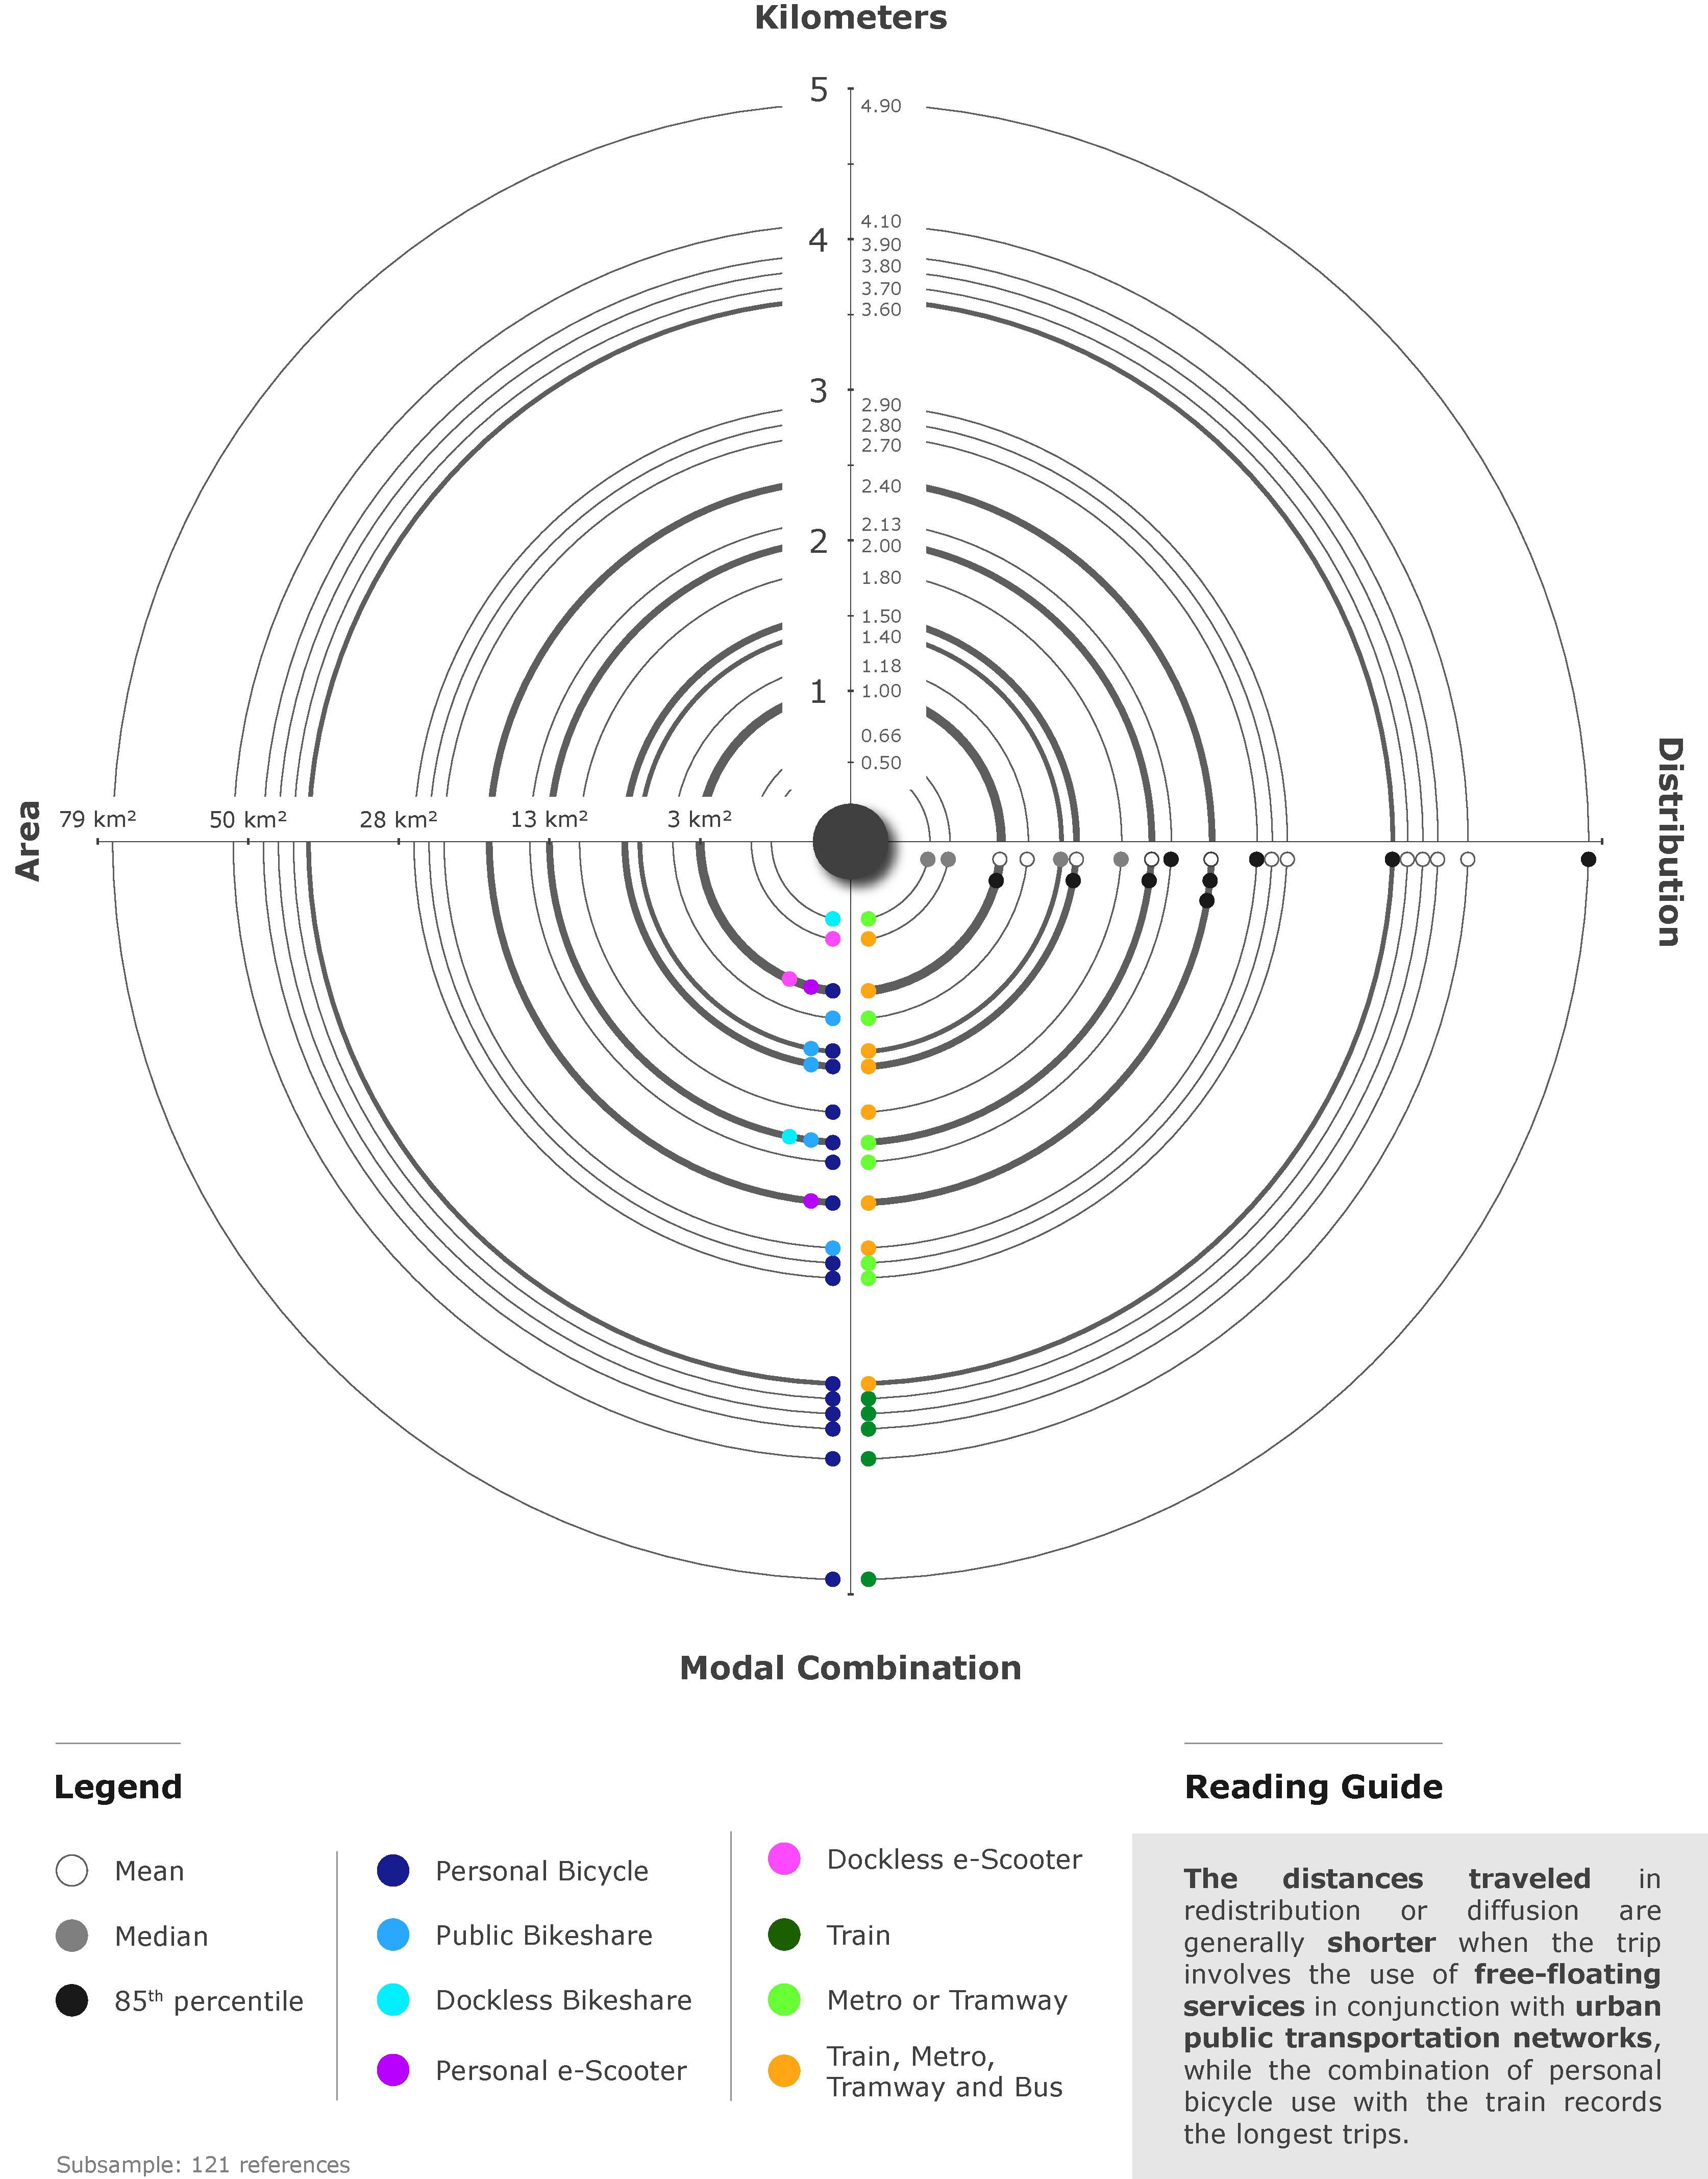
\includegraphics[width=1\columnwidth]{src/Figures/Chap-2/EN_RSL_Aires_influence.pdf}}
    \vspace{5pt}
    \begin{flushright}\scriptsize{
    Author: \textcolor{blue}{Dylan Moinse (2023)}
    }\end{flushright}
\end{figure}

% Distances time
Time-distance related to intermodality is a less explored aspect in the scientific literature, but a few studies provide important insights into the duration of trips combining light individual mobility and public transport. In Shanghai, \textcolor{blue}{\textcite[19]{lin_analysis_2019}}\index{Lin, Diao|pagebf}\index{Zhang, Yongping|pagebf}\index{Zhu, Ruoxin|pagebf}\index{Meng, Liqiu|pagebf} evaluate the average duration of a trip in \acrshort{DBS} to access a subway station as 8.2 minutes, equivalent to two kilometers. In Utrecht, trips by personal bike to and from public transport stations reveal distinct median durations: for access to the stations, the median duration is 10.1 minutes, corresponding to a distance of 1.8 kilometers, while for egress from the stations, it reaches 12.5 minutes, or a distance of 2.4 kilometers, according to \textcolor{blue}{\textcite[268]{krygsman_multimodal_2004}}\index{Krygsman, Stephan|pagebf}\index{Dijst, Martin|pagebf}\index{Arentze, Theo|pagebf}. In the Provence-Alpes-Côte d'Azur region, \textcolor{blue}{\textcite[186]{moinse_intermodal_2022}}\index{Moinse, Dylan|pagebf}\index{Goudeau, Matthieu|pagebf}\index{L'Hostis, Alain|pagebf}\index{Leysens, Thomas|pagebf} observe an average trip duration in \acrshort{PeS} of 10.6 minutes in combination with the train, equivalent to a distance of 2.4 kilometers. The use of \acrshort{PBS} in combination with the subway and bus presents an average travel time of 16 minutes, as shown in the case study on Taipei \textcolor{blue}{\autocite[49]{lu_improving_2018}}\index{Lu, Miaojia|pagebf}\index{Hsu, Shu Chien|pagebf}\index{Chen, Pi Cheng|pagebf}\index{Lee, Wan Yu|pagebf}, while this combination reaches a maximum value (95\textsuperscript{th} percentile) of 30 minutes in Nanjing \textcolor{blue}{\autocite[64]{ma_understanding_2018}}\index{Ma, Xinwei|pagebf}\index{Ji, Yanjie|pagebf}\index{Yang, Mingyuan|pagebf}\index{Jin, Yuchuan|pagebf}\index{Tan, Xu|pagebf}.%%Translated%%

% 2.3.5.4. Influence areas
\subsubsection*{Influence Areas
    \label{chap2:aires-influence}
    }

% <3km
The reviewed documentation is based on a defined study perimeter based on the distribution of spatial distances. In this regard, several academic studies have identified areas of influence with relatively limited reach, primarily focusing on public transport stops in urban areas. Thus, \textcolor{blue}{\textcite[5]{wang_interchange_2016}}\index{Wang, Zi-jia|pagebf}\index{Chen, Feng|pagebf}\index{Xu, Tian-kun|pagebf} observed that cycling distances in Beijing are mainly between 0.4 and 1.4 kilometers. According to the work of \textcolor{blue}{\textcite[11]{hu_examining_2022}}\index{Hu, Songhua|pagebf}\index{Chen, Mingyang|pagebf}\index{Jiang, Yuan|pagebf}\index{Sun, Wei|pagebf}\index{Xiong, Chenfeng|pagebf}, the relevant spatial distance for modeling the use of \acrshort{DBS} in Shanghai ranges from 1 to 1.5 kilometers, with suburban areas generally characterized by longer trips. This same influence perimeter is also adopted by \textcolor{blue}{\textcite[9]{jin_competition_2019}}\index{Jin, Haitao|pagebf}\index{Jin, Fengjun|pagebf}\index{Wang, Jiao'e|pagebf}\index{Sun, Wei|pagebf}\index{Dong, Libo|pagebf} and by \textcolor{blue}{\textcite[10]{fan_how_2019}}\index{Fan, Aihua|pagebf}\index{Chen, Xumei|pagebf}\index{Wan, Tao|pagebf} in the urban context of Beijing, suggesting an action radius of up to two kilometers for \acrshort{DBS}. In Shanghai, \textcolor{blue}{\textcite[185]{pan_intermodal_2010}}\index{Pan, Haixiao|pagebf}\index{Shen, Qing|pagebf}\index{Xue, Song|pagebf} determine an area ranging from 0.8 to 2.5 kilometers, emphasizing that the majority of bicycle and \acrshort{e-Bike} trips occur within distances less than 1.5 kilometers. According to \textcolor{blue}{\textcite[5]{ma_connecting_2022}}\index{Ma, Qingyu|pagebf}\index{Xin, Yanan|pagebf}\index{Yang, Hong|pagebf}\index{Xie, Kun|pagebf}, a perimeter between two and three kilometers was established to assess the reach of \acrshort{DESS} in Washington, D.C., with a similar approach observed in Beijing for \acrshort{DBS} \textcolor{blue}{\autocite[6]{ma_connecting_2022}}\index{Ma, Qingyu|pagebf}\index{Xin, Yanan|pagebf}\index{Yang, Hong|pagebf}\index{Xie, Kun|pagebf} as well as in Atlanta for cycling \textcolor{blue}{\autocite[57]{bearn_adaption_2018}}\index{Bearn, Cary|pagebf}\index{Mingus, Charlene|pagebf}\index{Watkins, Kari|pagebf}. It should be noted that the distance thresholds mentioned specifically relate to urban public transport networks, such as the subway. Therefore, the spatial configuration of these transport infrastructures, characterized by short distances between stations, can explain the small size of the measured influence areas.%%Translated%%

% >3km
From a radius of two to three kilometers, the considered geographical areas are more suitable for intermodal use of cycling combined with the train. Through an investigation in the Netherlands, \textcolor{blue}{\textcite[227]{keijer_how_2000}}\index{Keijer, Majanka|pagebf}\index{Rietveld, Piet|pagebf} and \textcolor{blue}{\textcite[73]{rietveld_accessibility_2000}}\index{Rietveld, Piet|pagebf} introduce a framework based on distance decay factors, thus justifying the establishment of an extended perimeter of 1 to 3.5 kilometers, beyond which the attraction to cycle usage tends to decrease. This observation is corroborated by the work of \textcolor{blue}{\textcite[281]{debrezion_modelling_2009}}\index{Debrezion, Ghebreegziabiher|pagebf}\index{Pels, Eric|pagebf}\index{Rietveld, Piet|pagebf}, which confirms that cycling is competitive for distances ranging from 1.1 to 4.2 kilometers to or from the station. Various scholarly works extend the influence area up to five kilometers, as evidenced by the use of \acrshort{DBS} in Shenzhen \textcolor{blue}{\autocite[6]{wu_measuring_2019}}\index{Wu, Xueying|pagebf}\index{Lu, Li|pagebf}\index{Lin, Yaoyu|pagebf}\index{Yang, Yiyang|pagebf}, or the combination of \acrshort{PBS} and cycling with the metro in Beijing \textcolor{blue}{\autocite[54]{zhao_bicycle-metro_2017}}\index{Zhao, Pengjun|pagebf}\index{Li, Shengxiao|pagebf}. The same impact zone is identified concerning the combination of cycling and the train, whether in Amboise \textcolor{blue}{\autocite[751]{midenet_modal_2018}}\index{Midenet, Sophie|pagebf}\index{Côme, Etienne|pagebf}\index{Papon, Francis|pagebf}, in Göteborg, Malmö, and Beijing \textcolor{blue}{\autocite[15]{hamidi_shaping_2020}}\index{Hamidi, Zahra|pagebf}\index{Zhao, Chunli|pagebf}, in El Monte \textcolor{blue}{\autocite[118]{cottrell_transforming_2007}}\index{Cottrell, Wayne~D.|pagebf}, or in Xi'an \textcolor{blue}{\autocite[172]{yang_bike-and-ride_2014}}\index{Yang, Liu|pagebf}\index{Chao, Li|pagebf}\index{Wang, Yuanqing|pagebf}. Going even further, \textcolor{blue}{\textcite[9]{kim_analysis_2021}}\index{Kim, Minjun|pagebf}\index{Cho, Gi-Hyoung|pagebf} support that trips combining \acrshort{PBS} and the metro in Seoul are frequent up to a distance of ten kilometers, thus highlighting the extended reach of these intermodal practices.%%Translated%%

% Temps
From a temporal perspective, part of the academic documentation has focused on determining the influence areas of public transport stations, taking the temporal variable into account. In this regard, \textcolor{blue}{\textcite[18, 21]{li_factors_2020}}\index{Li, Xuefeng|pagebf}\index{Du, Mingyang|pagebf}\index{Yang, Jingzong|pagebf} highlighted that \acrshort{DBS} trips lasting less than seven minutes predominate, especially during morning peak periods on weekdays, although some regions of Shenzhen, including its city center, show a majority of trips exceeding fifteen minutes. According to \textcolor{blue}{\textcite[128]{liu_understanding_2020}}\index{Liu, Yang|pagebf}\index{Ji, Yanjie|pagebf}\index{Feng, Tao|pagebf}\index{Timmermans, Harry~J.~P.|pagebf}, a biking duration of more than ten minutes reduces its use in combination with the metro in Nanjing. This duration is set at twelve minutes for the joint use of \acrshort{PBS} and the rail network in Boston, Chicago, Washington~D.C., and New York City \textcolor{blue}{\autocite[9]{kong_deciphering_2020}}\index{Kong, Hui|pagebf}\index{Jin, Scarlett~T.|pagebf}\index{Sui, Daniel~Z.|pagebf}, and extends to fifteen minutes for \acrshort{PBS} combined with the train in Osaka \textcolor{blue}{\autocite[3415]{tomita_demand_2017}}\index{Tomita, Yasuo|pagebf}\index{Nakayama, Akihiko|pagebf}. \textcolor{blue}{\textcite[5]{yang_empirical_2016}}\index{Yang, Min|pagebf}\index{Liu, Xinlu|pagebf}\index{Wang, Wei|pagebf}\index{Li, Zhibin|pagebf}\index{Zhao, Jingyao|pagebf} define a temporal perimeter of twenty minutes for the use of \acrshort{PBS} in relation to the metro network in Nanjing. Finally, \textcolor{blue}{\textcite[1696]{cheng_evaluating_2012}}\index{Cheng, Yung-Hsiang|pagebf}\index{Liu, Kuo-Chu|pagebf} adopt a more systemic approach by simultaneously measuring travel times for both feeder and egress trips, observing that the majority of cyclists using the metro in Kaohsiung make round trips of less than thirty minutes.%%Translated%%

% 2.3.5.5. Variability of Distances and Detours
\subsubsection*{Variability of Distances
    \label{chap2:variabilite-distances}
    }

    % Facteurs
The evaluation of the actual distances traveled by intermodal travelers, particularly for the \Commas{first and last miles,} is closely linked to the route choices made. These trips, taken by cyclists, are influenced by a variety of factors related to the urban environment, temporal context, as well as behaviors, habits, and mobility experiences. According to \textcolor{blue}{\textcite[15]{tzouras_describing_2023}}\index{Tzouras, Panagiotis|pagebf}\index{Mitropoulos, Lambros|pagebf}\index{Koliou, Katerina|pagebf}\index{Stavropoulou, Eirini|pagebf}\index{Karolemeas, Christos|pagebf}\index{Antoniou, Eleni|pagebf}\index{Karaloulis, Antonis|pagebf}\index{Mitropoulos, Konstantinos|pagebf}\index{Vlahogianni, Eleni~I.|pagebf}\index{Kepaptsoglou, Konstantinos|pagebf}, users of \acrshort{PeS} in Athens select their routes considering perceived safety and minimum distance, aiming to balance the required physical effort and the physical and psychological barriers to avoid. \textcolor{blue}{\textcite[621]{krizek_detailed_2007}}\index{Krizek, Kevin~J.|pagebf}\index{El-Geneidy, Ahmed~M.|pagebf}\index{Thompson, Kristin|pagebf} observe that the measured distances are also determined by the purpose of the trip: bike and tram journeys associated with shopping and work are shorter, while those related to leisure are longer, in Minneapolis. The environmental and temporal context also has a notable impact on the distances traveled. In this regard, \textcolor{blue}{\textcite[619]{krizek_detailed_2007}}\index{Krizek, Kevin~J.|pagebf}\index{El-Geneidy, Ahmed~M.|pagebf}\index{Thompson, Kristin|pagebf} show that cyclists are willing to extend their journey by up to 67\% to reach a high-quality bike path. \textcolor{blue}{\textcite[8]{adnan_last-mile_2019}}\index{Adnan, Muhammad|pagebf}\index{Altaf, Shahbaz|pagebf}\index{Bellemans, Tom|pagebf}\index{Yasar, Ansar-ul-Haque|pagebf}\index{Shakshuki, Elhadi~M.|pagebf} demonstrated that \acrshort{PBS} users in medium-sized cities in Belgium are sensitive to weather factors such as temperature and rainfall, influencing not only their routes but also their modal choices. \textcolor{blue}{\textcite[3110]{cho_estimation_2022}}\index{Cho, Shin-Hyung|pagebf}\index{Shin, DongHwa|pagebf} found that \acrshort{PBS} users in Seoul are more sensitive to distance in the evening compared to other times of the day. In Nanjing, \textcolor{blue}{\textcite[11]{li_operating_2019}}\index{Li, Yuan|pagebf}\index{Zhu, Zhenjun|pagebf}\index{Guo, Xiucheng|pagebf} revealed that the reach of \acrshort{DBS} varies depending on the day of the week and the type of metro station. These findings are consistent with those of \textcolor{blue}{\textcite[105]{flamm_public_2014}}\index{Flamm, Bradley~J.|pagebf}\index{Rivasplata, Charles~R.|pagebf}, who noted that the distances traveled by cyclists in Philadelphia and San Francisco depend on the type of public transport and the topography. Additionally, trains cover longer distances compared to conventional and express bus services, representing a more significant variable than socio-demographic factors, which have a moderate impact on distance in several U.S. cities \textcolor{blue}{\autocite[23-24]{hochmair_assessment_2015}}\index{Hochmair, Hartwig~H.|pagebf}. Finally, metro stations located on the outskirts of Shanghai have significantly larger catchment areas than those in the city center \textcolor{blue}{\autocite[8]{yu_policy_2021}}\index{Yu, Qing|pagebf}\index{Li, Weifeng|pagebf}\index{Yang, Dongyuan|pagebf}\index{Xie, Yingkun|pagebf}. This variety of factors affecting the relationship with distance illustrates how cyclists do not always prioritize the shortest route, revealing strategies aimed at balancing spatial-temporal optimization with comfort.%%Translated%%

% Détours
Several research studies highlight the practice of detours by intermodal travelers, who cover longer distances due to multiple factors. According to \textcolor{blue}{\textcite[102]{kampen_understanding_2020}}\index{Kampen, Jullian van|pagebf}\index{Jayaraj, Manoj Ashvin|pagebf}\index{Pauwels, Eric|pagebf}\index{Mei, Rob van der|pagebf}\index{Dugundji, Elenna~R.|pagebf}, 42\% of cyclists are inclined to head towards more distant stations rather than the nearest station, favoring those with better connectivity, in the regions of North-Holland, South-Holland, Flevoland, and Utrecht. On the one hand, \textcolor{blue}{\textcite[18]{jonkeren_bicycle-train_2021}}\index{Jonkeren, Olaf|pagebf}\index{Kager, Roland|pagebf}\index{Harms, Lucas|pagebf}\index{te Brömmelstroet, Marco|pagebf} emphasize the goal of bypassing transfer breaks by favoring stations with better facilities, such as those in Utrecht, Rotterdam, and Eindhoven. On the other hand, this preference also extends to metro stations offering bicycle parking facilities, as shown in the case study conducted by \textcolor{blue}{\textcite[342]{kampen_bicycle_2021}}\index{Kampen, Jullian van|pagebf}\index{Pauwels, Eric|pagebf}\index{Mei, Rob van der|pagebf}\index{Dugundji, Elenna~R.|pagebf} in Amsterdam. In Shanghai, \textcolor{blue}{\textcite[7]{li_exploring_2021}}\index{Li, Wenxiang|pagebf}\index{Chen, Shawen|pagebf}\index{Dong, Jieshuang|pagebf}\index{Wu, Jingxian|pagebf} reveal that the busiest public transport stations attract \acrshort{DBS} passengers from farther away. \textcolor{blue}{\textcite[143]{kampen_understanding_2021}}\index{Kampen, Jullian van|pagebf}\index{Jayaraj, Manoj Ashvin|pagebf}\index{Pauwels, Eric|pagebf}\index{Mei, Rob van der|pagebf}\index{Dugundji, Elenna~R.|pagebf} add that cyclists with a net monthly income of less than~\euro2,500 and aged over 39 are more likely to go to the second nearest station to their departure point. The role of factors influencing the actual distances traveled reflects the importance of policies and strategies aimed at guiding people's mobility to make alternative mobility systems more attractive compared to car use.%%Translated%%

% 2.3.6. Resultats : management de la demande
\subsection{Mobility Demand Management
    \label{chap2:gestion-demande-mobilite}
    }

    % Introduction
Mobility demand management, encompassing all strategies and policies aimed at influencing individuals' travel choices, is at the core of 61 scientific studies addressing \acrshort{M-TOD}. Our analysis will begin by examining the role of the service level offered by public transport systems and the importance of implementing integrated pricing. We will then discuss the contribution of shared mobility services, as well as the role of bus networks in transit-oriented neighborhoods. Finally, this section will address traffic and parking management.%%Translated%%

% 2.3.6.1. Fréquence et temps d'attente
\subsubsection*{Mass Transit Service Level
    \label{chap2:niveau-service}
    }

    % Frequency of public transport
A regular and punctual rail service seems to favor the use of bicycles in intermodal travel. This observation has been noted for trains in the Randstad South \textcolor{blue}{\autocite[45]{la_paix_puello_modelling_2015}}\index{La Paix Puello, Lissy|pagebf}\index{Geurs, Karst~T.|pagebf}, Rotterdam \textcolor{blue}{\autocite[5]{montes_shared_2023}}\index{Montes, Alejandro|pagebf}\index{Geržinic, Nejc|pagebf}\index{Veeneman, Wijnand|pagebf}\index{Oort, Niels van|pagebf}\index{Hoogendoorn, Serge|pagebf}, Turin \textcolor{blue}{\autocite[12]{staricco_implementing_2020}}\index{Staricco, Luca|pagebf}\index{Vitale Brovarone, Elisabetta|pagebf}, and Shanghai for the \acrshort{DBS} in combination with the metro \textcolor{blue}{\autocite[24]{lin_analysis_2019}}\index{Lin, Diao|pagebf}\index{Zhang, Yongping|pagebf}\index{Zhu, Ruoxin|pagebf}\index{Meng, Liqiu|pagebf}. In Melbourne, \textcolor{blue}{\textcite[401]{weliwitiya_bicycle_2019}}\index{Weliwitiya, Hesara|pagebf}\index{Rose, Geoff|pagebf}\index{Johnson, Marilyn|pagebf} highlighted a positive correlation between the frequency of rail lines, particularly during the morning peak hours, and the use of bicycles as a feeder mode. The authors found that an increase of one unit in frequency led to an increase of 1.03 in the number of intermodal cyclists. In Poznań, \textcolor{blue}{\textcite[199]{radzimski_exploring_2021}}\index{Radzimski, Adam|pagebf}\index{Dzięcielski, Michał|pagebf} demonstrated a positive correlation between the frequency of tram lines and the number of \acrshort{PBS} trips for short distances, up to 1.5 kilometers, and for medium distances, between 1.5 and 3 kilometers. However, this relationship was not observed for trips exceeding 3 kilometers. However, \textcolor{blue}{\textcite[301]{kuijk_preferences_2022}}\index{Mil, Joeri~F.P. van|pagebf}\index{Leferink, Tessa~S.|pagebf}\index{Annema, Jan Anne|pagebf}\index{Oort, Niels van|pagebf}\index{Kuijk, Roy~J. van|pagebf}\index{Almeida Correia, Gonçalo Homem de|pagebf}\index{Oort, Niels van|pagebf}\index{Arem, Bart van|pagebf} did not identify any significant parameters concerning the frequency and speed of trams related to the use of \acrshort{PBS} in Utrecht. Moreover, the results of studies by \textcolor{blue}{\textcite[41]{nielsen_bikeability_2018}}\index{Nielsen, Thomas Alexander Sick|pagebf}\index{Skov-Petersen, Hans|pagebf} suggest that the frequency of rail services might decrease the likelihood of using bicycles in Denmark.%%Translated%%

% Station density
Beyond the frequency of public transport services, the commercial speed of these collective modes, intrinsically linked to travel time, proves to be a key factor in modal choice favoring the bicycle. This trend contrasts with the minor role attributed to the punctuality and safety of rail services in Eindhoven \textcolor{blue}{\autocite[727]{waerden_relation_2018}}\index{Waerden, Peter|pagebf}\index{Waerden, Jaap|pagebf}. The speed of public transport journeys is largely influenced by the density of stations, which has a significant impact on the demand for bike transfers. Indeed, very close train stations tend to reduce the likelihood of opting for this mode of transport in Denmark \textcolor{blue}{\autocite[41]{nielsen_bikeability_2018}}\index{Nielsen, Thomas Alexander Sick|pagebf}\index{Skov-Petersen, Hans|pagebf}. In contrast, the density of metro stations positively affects the use of \acrshort{PBS} in Nanjing \textcolor{blue}{\autocite[17]{ji_exploring_2018}}\index{Ji, Yanjie|pagebf}\index{Ma, Xinwei|pagebf}\index{Yang, Mingyuan|pagebf}\index{Jin, Yuchuan|pagebf}\index{Gao, Liangpeng|pagebf}. Exploring the combination of \acrshort{DBS} and metro in Beijing, \textcolor{blue}{\textcite[10]{guo_exploring_2023}}\index{Guo, Dongbo|pagebf}\index{Yao, Enjian|pagebf}\index{Liu, Shasha|pagebf}\index{Chen, Rongsheng|pagebf}\index{Hong, Junyi|pagebf}\index{Zhang, Junyi|pagebf} found that waiting time has a much more negative impact than travel time itself—users are willing to pay~\euro13.6 (CNY~105) to save an hour of waiting time, compared to~\euro2 (CNY~15) for an hour of \acrshort{DBS}—highlighting the need to establish efficient connections within the public transport system to address the aversion to transfer times.%%Translated%%

% 2.3.6.2. MaaS and pricing
\needspace{1\baselineskip} % Reserve space
\subsubsection*{Integrated pricing
    \label{chap2:tarification_integree}
    }

% MaaS
To promote integration and encourage intermodal practices, the scientific literature recommends simplifying the connections between different mobility systems by promoting the use of integrated transport cards \textcolor{blue}{\autocite[172]{yang_bike-and-ride_2014}}\index{Yang, Liu|pagebf}\index{Chao, Li|pagebf}\index{Wang, Yuanqing|pagebf}, the most popular option among passengers \textcolor{blue}{\autocite[10]{yang_empirical_2016}}\index{Yang, Min|pagebf}\index{Liu, Xinlu|pagebf}\index{Wang, Wei|pagebf}\index{Li, Zhibin|pagebf}\index{Zhao, Jingyao|pagebf}. One of the main levers identified is shared light individual mobility and the implementation of a multimodal platform like \acrshort{MaaS}, offering the possibility of pooling or even unifying online payments \textcolor{blue}{\autocite[5]{fearnley_patterns_2020}}\index{Fearnley, Nils|pagebf}\index{Johnsson, Espen|pagebf}\index{Berge, Siri Hegna|pagebf}. In Nanjing, a lack of information about bike rental facilities has been noted, despite clear interest in the service, highlighting the importance of \acrshort{MaaS} \textcolor{blue}{\autocite[136]{chen_determinants_2012}}\index{Chen, Lijun|pagebf}\index{Pel, Adam~J.|pagebf}\index{Chen, Xuewu|pagebf}\index{Sparing, Daniel|pagebf}\index{Hansen, Ingo~A.|pagebf}. According to \textcolor{blue}{\textcite[67]{ma_understanding_2018}}\index{Ma, Xinwei|pagebf}\index{Ji, Yanjie|pagebf}\index{Yang, Mingyuan|pagebf}\index{Jin, Yuchuan|pagebf}\index{Tan, Xu|pagebf}, integrated platforms should include a loyalty program to prioritize frequent \acrshort{PBS} and public transport users by reserving bike-sharing locations for these users. However, \textcolor{blue}{\textcite[12]{fan_how_2019}}\index{Fan, Aihua|pagebf}\index{Chen, Xumei|pagebf}\index{Wan, Tao|pagebf} highlight barriers to using the \acrshort{DBS} or a \acrshort{MaaS} platform in Beijing, such as the need to install a mobile app, provide personal information for registration, and pay a large deposit, while pricing remains the main factor influencing the choice of \acrshort{DBS}.%%Translated%%

% Bike-sharing and shared micromobility pricing
The costs of bike-sharing and shared micromobility are often deemed prohibitive, discouraging their use for first- and last-mile trips, and even more so for long-distance trips \textcolor{blue}{\autocite[5]{montes_shared_2023}}\index{Montes, Alejandro|pagebf}\index{Geržinic, Nejc|pagebf}\index{Veeneman, Wijnand|pagebf}\index{Oort, Niels van|pagebf}\index{Hoogendoorn, Serge|pagebf}. In Nanjing, young workers choose \acrshort{PBS} for economic reasons, raising questions about pricing strategies that do not encourage the long-term use of these sustainable mobility practices. In this regard, the costs of a single trip and a subscription to the service have a significant impact on the choice of \acrshort{DBS} to access the metro network \textcolor{blue}{\autocite[17]{zhong_layout_2021}}\index{Zhong, Hongming|pagebf}\index{Liu, Zijian|pagebf}\index{Chen, Jun|pagebf}\index{Hao, Jun|pagebf}\index{Wang, Wei|pagebf}. In Beijing, travelers using \acrshort{DBS} spend almost as much on short trips using this service as they do on public transport \textcolor{blue}{\autocite[12]{fan_how_2019}}\index{Fan, Aihua|pagebf}\index{Chen, Xumei|pagebf}\index{Wan, Tao|pagebf}. Several solutions emerge from these findings. In Nanjing, a free two-hour bike rental policy, as an effective promotional strategy for 57\% of travelers, has been identified by \textcolor{blue}{\textcite[135]{chen_determinants_2012}}\index{Chen, Lijun|pagebf}\index{Pel, Adam~J.|pagebf}\index{Chen, Xuewu|pagebf}\index{Sparing, Daniel|pagebf}\index{Hansen, Ingo~A.|pagebf}. In Washington D.C. and Los Angeles, pricing incentives favoring the use of \acrshort{DESS} with the metro are being evaluated, including price reductions when a~\euro2.8 (\$3) credit is applied to scooter fares \textcolor{blue}{\autocite[11]{yan_evaluating_2023}}\index{Yan, Xiang|pagebf}\index{Zhao, Xilei|pagebf}\index{Broaddus, Andrea|pagebf}\index{Johnson, Joshua|pagebf}\index{Srinivasan, Sivaramakrishnan|pagebf}. In Boston and Worcester, the impact of different pricing schemes is analyzed, revealing that a combination of a fixed fare and distance-based fare has the least impact on the demand for bike and train combinations \textcolor{blue}{\autocite[16]{fournier_continuous_2021}}\index{Fournier, Nicholas|pagebf}\index{Christofa, Eleni|pagebf}\index{Gonzales, Eric~J.|pagebf}, while in Oslo, the price per minute is an important factor in promoting the use of \acrshort{DESS} with public transport \textcolor{blue}{\autocite[5]{fearnley_patterns_2020}}\index{Fearnley, Nils|pagebf}\index{Johnsson, Espen|pagebf}\index{Berge, Siri Hegna|pagebf}. A social pricing scheme based on income is considered effective for \acrshort{DBS} and \acrshort{DESS} in Seattle to alleviate financial barriers \textcolor{blue}{\autocite[975-977]{beale_integrating_2023}}\index{Beale, Kirsten|pagebf}\index{Kapatsila, Bogdan|pagebf}\index{Grisé, Emily|pagebf}.%%Translated%%

% Pricing for public transport and bike parking
Finally, monetary cost also affects the use of public transport as well as bike and micromobility parking. The free access to rail services targeted at students in the Netherlands attracts more intermodal cyclists at the expense of automobiles \textcolor{blue}{\autocite[360]{givoni_access_2007}}\index{Givoni, Moshe|pagebf}\index{Rietveld, Piet|pagebf}. A significant aversion to bike parking fees is observed among Dutch students \textcolor{blue}{\autocite[667]{mil_insights_2020}}\index{Mil, Joeri~F.P. van|pagebf}\index{Leferink, Tessa~S.|pagebf}\index{Annema, Jan Anne|pagebf}\index{Oort, Niels van|pagebf}. However, \textcolor{blue}{\textcite[10]{molin_bicycle_2015}}\index{Molin, Eric|pagebf}\index{Maat, Kees|pagebf} indicate that free bike parking does not influence the use of bikes for intermodality in the Netherlands, and on the contrary, 65\% of the cyclists surveyed prefer the scenario based on secure, paid parking with an optimal price of 1.50\euro. Similarly, \textcolor{blue}{\textcite[5]{liu_mode_2022}}\index{Liu, Lumei|pagebf}\index{Kong, Hui|pagebf}\index{Liu, Tianliang|pagebf}\index{Ma, Xiaolei|pagebf} find that the cost of the trip has little impact on the choice between the bus or \acrshort{DBS} when transferring with the metro in Beijing, suggesting that the quality of bike-sharing infrastructure is a more important factor to consider.%%Translated%%

% 2.3.6.3. Shared Bike and micromobility Services
\subsubsection*{Transfer Services
    \label{chap2:services-transfert}
    }

% Presence of bike-sharing
The availability of shared mobility systems, such as \acrshort{PBS}, \acrshort{DBS}, or \acrshort{DESS}, is a fundamental element for integrating bicycles with public transport \textcolor{blue}{\autocite[11-12]{wu_measuring_2019}}\index{Wu, Xueying|pagebf}\index{Lu, Li|pagebf}\index{Lin, Yaoyu|pagebf}\index{Yang, Yiyang|pagebf}. Thus, the incorporation of these mobility services within the urban \acrshort{TOD} strategy is recommended to increase the use and overall efficiency of the mobility system \textcolor{blue}{\autocite[16]{tamakloe_determinants_2021}}\index{Tamakloe, Reuben|pagebf}\index{Hong, Jungyeol|pagebf}\index{Tak, Jihoon|pagebf}. The availability of bikes and micromobility options in bike-sharing systems close to transport hubs not only increases the probability of their use as connection modes \textcolor{blue}{\autocite[25]{guo_dockless_2021}}\index{Guo, Yuanyuan|pagebf}\index{Yang, Linchuan|pagebf}\index{Lu, Yi|pagebf}\index{Zhao, Rui|pagebf}, but these systems also contribute to promoting more efficient intermodal travel practices, reducing the need for a second bike \textcolor{blue}{\autocite[10]{jonkeren_bicycle_2021}}\index{Jonkeren, Olaf|pagebf}\index{Kager, Roland|pagebf}. In Shanghai, \textcolor{blue}{\textcite[186]{pan_intermodal_2010}}\index{Pan, Haixiao|pagebf}\index{Shen, Qing|pagebf}\index{Xue, Song|pagebf} identified a strong willingness expressed by study participants to use bike rental systems near metro stations. Based on the observation that intermodal travelers have a high degree of trip planning and adapt their behavior according to mobility offerings and constraints related to transport and bike parking, \textcolor{blue}{\textcite[196]{sherwin_practices_2011}}\index{Sherwin, Henrietta|pagebf}\index{Parkhurst, Graham|pagebf}\index{Robbins, Derek|pagebf}\index{Walker, Ian|pagebf} justify the establishment of a nationwide organized bike rental system, similar to what is practiced by Dutch and German railway operators.%%Translated%%

% Management and Redistribution of Shared Bike and micromobility Services
The implementation of a shared light individual mobility system requires efficient management and optimal fleet distribution. The work of \textcolor{blue}{\textcite[197]{radzimski_exploring_2021}}\index{Radzimski, Adam|pagebf}\index{Dzięcielski, Michał|pagebf} demonstrates that structuring a \acrshort{PBS} system, organized in the form of dockless bikes with dedicated stations, attracts more users in combination with trams compared to \acrshort{DBS}. Therefore, it is recommended to improve the allocation of \acrshort{DBS} by more efficiently redistributing bikes towards green spaces, commercial and industrial areas, as well as residential neighborhoods in Beijing \textcolor{blue}{\autocite[12]{liu_temporal_2022}}\index{Liu, Siyang|pagebf}\index{Zhang, Xiaodong|pagebf}\index{Zhou, Chenjing|pagebf}\index{Rong, Jian|pagebf}\index{Bian, Yang|pagebf}. Given the capacity limitations of dockless sharing systems during usage peaks, as observed for \acrshort{DESS} in Columbus \textcolor{blue}{\autocite[9]{liu_measuring_2022}}\index{Liu, Luyu|pagebf}\index{Miller, Harvey~J.|pagebf}, \textcolor{blue}{\textcite[69, 95]{nat_bicycle_2018}}\index{Nat, Johanna Debóra van der|pagebf} suggests an alternative bike-sharing model. This model relies on a combination of rental and sufficient availability of shared bikes to ensure their accessibility and maximize parking space savings in Amsterdam.%%Translated%%

% Embarkation / Carrying in Public Transport
The establishment of efficient connections between public transport systems and light individual mobility is also reflected in the ease of carrying bikes and micromobility devices aboard public transport modes. Combined with the implementation of an effective bike-sharing and micromobility service system and parking facilities, the boarding of light individual mobility in public transport vehicles stimulates intermodal practices in Portland \textcolor{blue}{\autocite[93]{singleton_exploring_2014}}\index{Singleton, Patrick~A.|pagebf}\index{Clifton, Kelly~J.|pagebf}. In Copenhagen, \textcolor{blue}{\textcite[19]{halldorsdottir_home-end_2017}}\index{Halldórsdóttir, Katrín|pagebf}\index{Nielsen, Otto Anker|pagebf}\index{Prato, Carlo Giacomo|pagebf} demonstrate that the ability to transport a bike for free on the train increases the intermodal use of bicycles. Moreover, managing bike and micromobility interconnections should be considered in relation to bus services, as a substitution effect between \acrshort{PBS} and \acrshort{DBS} with the bus is observed in Nanjing \textcolor{blue}{\autocite[12]{chen_what_2022}}\index{Chen, Wendong|pagebf}\index{Chen, Xuewu|pagebf}\index{Chen, Jingxu|pagebf}\index{Cheng, Long|pagebf}.%%Translated%%

% Bus Service
\subsubsection*{Bus Service
    \label{chap2:desserte-bus}
    }

% Modal Substitution
Given the modal substitution effect between light individual mobility and buses, it appears that the density of bus stops in the area of influence of major public transport stations is inversely proportional to the use of these modes of transport. For example, in Beijing, bus services substitute for the use of bicycles, \acrshort{PBS} \textcolor{blue}{\autocite[55]{zhao_bicycle-metro_2017}}\index{Zhao, Pengjun|pagebf}\index{Li, Shengxiao|pagebf} and \acrshort{DBS} \textcolor{blue}{\autocite[16]{wang_spatiotemporal_2020}}\index{Wang, Zi-jia|pagebf}. \textcolor{blue}{\textcite[10]{li_exploring_2021}}\index{Li, Wenxiang|pagebf}\index{Chen, Shawen|pagebf}\index{Dong, Jieshuang|pagebf}\index{Wu, Jingxian|pagebf} observe that the density of bus stops decreases gradually as the transfer distance increases, providing a comparative advantage to \acrshort{DBS} when this distance exceeds a certain threshold in Shanghai. Similarly, \textcolor{blue}{\textcite[20]{luan_better_2020}}\index{Luan, Xin|pagebf}\index{Cheng, Lin|pagebf}\index{Song, Yan|pagebf}\index{Zhao, Jinbao|pagebf} find that residents of Nanjing tend to abandon the bus in favor of cycling, which could indicate dissatisfaction with existing bus services.%%Translated%%

% Absence of Modal Substitution
\textsl{A contrario}, a greater portion of studies seems to indicate an absence of modal substitution, revealing, on the contrary, that bus connections have a positive impact on the use of \acrshort{PBS} in combination with the train in Washington~D.C. \textcolor{blue}{\autocite[7-8]{ma_bicycle_2015}}\index{Ma, Ting|pagebf}\index{Liu, Chao|pagebf}\index{Erdoğan, Sevgi|pagebf} and \acrshort{DBS} with the metro in Shenzhen \textcolor{blue}{\autocite[12]{guo_built_2020}}\index{Guo, Yuanyuan|pagebf}\index{He, Sylvia~Y.|pagebf}. According to \textcolor{blue}{\textcite[20]{arbis_analysis_2016}}\index{Arbis, David|pagebf}\index{Hossein Rashidi, Taha|pagebf}\index{Dixit, Vinayak~V.|pagebf}\index{Vandebona, Upali|pagebf}, the presence of a bus stop near the stations is a predictive indicator of higher levels of bicycle parking usage in New South Wales. However, these reported conclusions may involve a misinterpretation of the data. Indeed, the observed correlation between the presence of bus stops and the increased use of bike-sharing could simply signal a better quality of service at the concerned stations, rather than establishing a direct cause-and-effect relationship. Furthermore, it is possible that these stations are located in areas where the development of bus stops coincides with policies aimed at reducing car space. While the mobility demand management aspect focuses on incentive measures—this section mainly addresses this dimension from the perspective of the level of service of collective modes, pricing, interconnection management, and bus service—competition with the automobile should not be overlooked, integrating a perspective on coercive policies. This approach should be considered to evaluate demand management strategies and their potential impact on promoting an alternative mobility system while reducing reliance on cars.%%Translated%%

% 2.3.6.5. Car
\needspace{1\baselineskip} % Réserve de l'espace
\subsubsection*{Moderation of Competitive Car Use
    \label{chap2:moderation-automobile}
    }

% Parking Reduction
In the context of urban development focused on the integration of public transport and light individual mobility, it is essential to consider the place of the car and highlight the importance of proactive policies to adapt public and private spaces to regulate traffic and motorized parking. A positive correlation is established between the increase in the motorization rate in an area and the increased use of cars to access stations in the Netherlands, with the car surpassing other modes of transfer starting from 0.60 cars per person for trips exceeding ten kilometers \textcolor{blue}{\autocite[281]{debrezion_modelling_2009}}\index{Debrezion, Ghebreegziabiher|pagebf}\index{Pels, Eric|pagebf}\index{Rietveld, Piet|pagebf}. In Provence-Alpes-Côte d'Azur, \textcolor{blue}{\autocite[190]{moinse_intermodal_2022}}\index{Moinse, Dylan|pagebf}\index{Goudeau, Matthieu|pagebf}\index{L'Hostis, Alain|pagebf}\index{Leysens, Thomas|pagebf} found that an intermodal trip takes a quarter more time than an equivalent car trip, excluding urban congestion and parking time, indicating the need for coercive measures if the competitiveness of cycling and \acrshort{PeS} with the train is to be increased.%%Translated%%

% Parking Recommendations
In Copenhagen, \textcolor{blue}{\textcite[18]{halldorsdottir_home-end_2017}}\index{Halldórsdóttir, Katrín|pagebf}\index{Nielsen, Otto Anker|pagebf}\index{Prato, Carlo Giacomo|pagebf} observed that the availability of car parking influences the choice of transfer modes to access stations. An increase of one hundred parking spaces around a station, typically equipped with 1,700 spaces, is linked to a 4\% decrease in walking and cycling usage, revealing a conflict between \acrfull{PnR} and \gls{active modes} in Toronto and Hamilton \textcolor{blue}{\autocite[2172-2173]{chan_factors_2020}}\index{Chan, Kevin|pagebf}\index{Farber, Steven|pagebf}. Furthermore, the saturation of parking lots around stations, and even more so at the destination, increases the likelihood of adopting active modes in the United States \textcolor{blue}{\autocite[4270]{bopp_examining_2015}}\index{Bopp, Melissa|pagebf}\index{Gayah, Vikash~V.|pagebf}\index{Campbell, Matthew~E.|pagebf}. Concerning egress from metro stations, it has been observed that the availability of parking spaces for motorcycles negatively influences passengers' intention to use \acrshort{PBS} in Kaohsiung \textcolor{blue}{\autocite[28]{cheng_expanding_2018}}\index{Cheng, Yung-Hsiang|pagebf}\index{Li, Yi-Chun|pagebf}. Therefore, it is suggested to strengthen regulations on the parking of motor vehicles around highly frequented stations to improve transportation demand management and enhance the competitiveness of combined cycling and metro in Xi'an \textcolor{blue}{\autocite[7]{zhu_improved_2021}}\index{Zhu, Zhenjun|pagebf}\index{He, Yudong|pagebf}\index{Guo, Xiucheng|pagebf}\index{Zhang, Yibang|pagebf}\index{Chen, Junlan|pagebf}. However, \textcolor{blue}{\textcite[401]{weliwitiya_bicycle_2019}}\index{Weliwitiya, Hesara|pagebf}\index{Rose, Geoff|pagebf}\index{Johnson, Marilyn|pagebf} warn against focusing solely on the car parking planned around stations without considering other types of parking, such as nearby streets or garages, which account for 72\% of the recorded parking for users arriving by car at the stations in Melbourne.%%Translated%%

% Parking Pricing
Beyond controlling access to parking, it has been shown that the introduction of BART in San Francisco led to an increase in parking fees around stations, which were previously free, thus encouraging bicycle usage \textcolor{blue}{\autocite[94]{cervero_bike-and-ride_2013}}\index{Cervero, Robert|pagebf}\index{Caldwell, Benjamin|pagebf}\index{Cuellar, Jesus|pagebf}. Several studies recommend better control of access to station parking through a pricing strategy inversely proportional to the transfer distance, as a lever for a powerful modal shift \textcolor{blue}{\autocite[751]{midenet_modal_2018}}\index{Midenet, Sophie|pagebf}\index{Côme, Etienne|pagebf}\index{Papon, Francis|pagebf}. In addition to car parking, \textcolor{blue}{\textcite[2737]{papon_evaluation_2017}}\index{Papon, Francis|pagebf}\index{Beauvais, Jean-Marie|pagebf}\index{Midenet, Sophie|pagebf}\index{Côme, Etienne|pagebf}\index{Polombo, Nadine|pagebf}\index{Abours, Sylvie|pagebf}\index{Belton-Chevallier, Leslie|pagebf}\index{Soulas, Claude|pagebf} conducted a socio-economic analysis showing that doubling the price of fuel would result in a 7\% increase in the modal share of cycling to stations.%%Translated%%

% 2.3.7. Results: Socio-demographic Profiles
\needspace{1\baselineskip} % Reserve space
\subsection{Socio-demographic Characteristics of Users
    \label{chap2:sociodemographie-usagers}
    }

    % Introduction
The revisited \acrshort{M-TOD} model, like any urban development strategy, must demonstrate its ability to promote inclusive accessibility. This means that it must not only improve sustainable access to territorial resources but also ensure that these improvements benefit all segments of the population equitably, including social groups that are often marginalized in urban planning. Consequently, this section is dedicated to an in-depth analysis of the socio-demographic characteristics of the population, with the goal of shaping an urban fabric that meets the specific needs of current and future users, while ensuring social inclusion. In this perspective, our study focuses on examining the various socio-demographic and economic dimensions that define the profiles of users of light individual mobility. This exploration, based on 90 scientific publications, will include not only an analysis of gender and age effects but also variables related to household composition, classifications based on \acrshort{PCS}, available income levels, educational attainment, and household equipment related to mobility.%%Translated%%

% 2.3.7.1.
\needspace{1\baselineskip} % Reserve space
\subsubsection*{Gender Effects
    \label{chap2:genre}
    }

    % Men and bicycles
From the outset, the scientific literature reports gender disparities that manifest in the modal choice of integrated light individual mobility. Men seem more inclined to use personal bicycles in conjunction with public transport networks. This trend is observed in various geographical contexts, such as the Netherlands \textcolor{blue}{\autocite[278]{debrezion_modelling_2009}}\index{Debrezion, Ghebreegziabiher|pagebf}\index{Pels, Eric|pagebf}\index{Rietveld, Piet|pagebf}, New Delhi \textcolor{blue}{\autocite[35]{mohanty_effect_2017}}\index{Mohanty, Sudatta|pagebf}\index{Bansal, Sugam|pagebf}\index{Bairwa, Khushi|pagebf}, and Mountain View \textcolor{blue}{\autocite[36]{park_finding_2014}}\index{Park, Sungjin|pagebf}\index{Kang, Junhee|pagebf}\index{Choi, Keechoo|pagebf}, except for Singapore \textcolor{blue}{\autocite[45]{meng_influence_2016}}\index{Meng, Meng|pagebf}\index{Koh, Puay Ping|pagebf}\index{Wong, Yiik Diew|pagebf} and Rio de Janeiro \textcolor{blue}{\autocite[62]{souza_modelling_2017}}\index{Souza, Flavia de|pagebf}\index{La Paix Puello, Lissy|pagebf}\index{Brussel, Mark|pagebf}\index{Orrico, Romulo|pagebf}. A substantial body of studies reveals gender inequalities in the use of combined cycling, with a majority of male users reported in Bristol \textcolor{blue}{\autocite[194]{sherwin_practices_2011}}\index{Sherwin, Henrietta|pagebf}\index{Parkhurst, Graham|pagebf}\index{Robbins, Derek|pagebf}\index{Walker, Ian|pagebf} and San Francisco \textcolor{blue}{\autocite[103]{flamm_public_2014}}\index{Flamm, Bradley~J.|pagebf}\index{Rivasplata, Charles~R.|pagebf}. In Kaohsiung, 58\% of cyclists heading to a subway station are men \textcolor{blue}{\autocite[1700]{cheng_evaluating_2012}}\index{Cheng, Yung-Hsiang|pagebf}\index{Liu, Kuo-Chu|pagebf}, and this proportion reaches two-thirds in Toronto and Hamilton \textcolor{blue}{\autocite[378]{ravensbergen_biking_2018}}\index{Ravensbergen, Léa|pagebf}\index{Buliung, Ron|pagebf}\index{Mendonca, Meaghan|pagebf}\index{Garg, Naren|pagebf}. In the regions of Delft, Zwolle, Midden-Delfland, and Pijnacker-Nootdorp, intermodal cyclists are predominantly male, contrasting with groups of car drivers, monomodal cyclists, and public transport users, who are more balanced \textcolor{blue}{\autocite[114]{heinen_multimodal_2014}}\index{Heinen, Eva|pagebf}\index{Bohte, Wendy|pagebf}. Moreover, men tend to make longer bike trips to reach a station in Utrecht \textcolor{blue}{\autocite[267]{krygsman_multimodal_2004}}\index{Krygsman, Stephan|pagebf}\index{Dijst, Martin|pagebf}\index{Arentze, Theo|pagebf}. Additionally, \textcolor{blue}{\autocite[107]{wang_bicycle-transit_2013}}\index{Wang, Rui|pagebf}\index{Liu, Chen|pagebf} found that in the United States, an overwhelming majority of intermodal trips involving cycling are made by men, and an increasing gender gap in usage was observed between 2001 and 2009. However, \textcolor{blue}{\autocite[59]{bearn_adaption_2018}}\index{Bearn, Cary|pagebf}\index{Mingus, Charlene|pagebf}\index{Watkins, Kari|pagebf} show that by focusing on expanding a \Commas{low-stress cycling network} toward isolated communities, these planning policies would increase women's access in Atlanta.%%Translated%%

% Men VLS+VFF
Regarding the intermodal use of the \acrshort{PBS}, a similar imbalance has been observed in Belgian cities with populations between 30,000 and 200,000 \textcolor{blue}{\autocite[6]{adnan_last-mile_2019}}\index{Adnan, Muhammad|pagebf}\index{Altaf, Shahbaz|pagebf}\index{Bellemans, Tom|pagebf}\index{Yasar, Ansar-ul-Haque|pagebf}\index{Shakshuki, Elhadi~M.|pagebf}, in Suzhou \textcolor{blue}{\autocite[9]{ma_measuring_2018}}\index{Ma, Xinwei|pagebf}\index{Jin, Yuchuan|pagebf}\index{He, Mingja|pagebf} as well as in Washington~D.C. and Minneapolis \textcolor{blue}{\autocite[322]{martin_evaluating_2014}}\index{Martin, Elliot~W.|pagebf}\index{Shaheen, Susan~A.|pagebf}. Similarly, \textcolor{blue}{\textcite[111]{bachand-marleau_much-anticipated_2011}}\index{Bachand-Marleau, Julie|pagebf}\index{Larsen, Jacob|pagebf}\index{El-Geneidy, Ahmed~M.|pagebf} observed a male predominance among \acrshort{PBS} users in Montreal, representing 58\% of travelers. Similarly, \textcolor{blue}{\textcite[393]{bocker_bike_2020}}\index{Böcker, Lars|pagebf}\index{Anderson, Ellinor|pagebf}\index{Uteng, Tanu Priya|pagebf}\index{Throndsen, Torstein|pagebf} revealed a gender distribution of 58\% male cyclists in Oslo, with a higher concentration in the city center. These authors further note that this proportion rises to 68\% for trips made, suggesting that men use the \acrshort{PBS} more frequently in combination with the metro than women. In Nanjing, \textcolor{blue}{\textcite[64]{ma_understanding_2018}}\index{Ma, Xinwei|pagebf}\index{Ji, Yanjie|pagebf}\index{Yang, Mingyuan|pagebf}\index{Jin, Yuchuan|pagebf}\index{Tan, Xu|pagebf} observed that women differ from men in their use of the \acrshort{PBS}, traveling more often between 6:00–7:00 AM and 4:00–5:00 PM, regularly after accompanying their children. Only one study, focused on the combination of the \acrshort{DBS} with public transport in Beijing, found that individuals identifying as men tend to favor these modes of travel 3.3 times more than individuals identifying as women \textcolor{blue}{\autocite[10]{fan_how_2019}}\index{Fan, Aihua|pagebf}\index{Chen, Xumei|pagebf}\index{Wan, Tao|pagebf}. Regarding the interrelation between gender issues and electric scooter use, \textcolor{blue}{\textcite[12]{pages_nouveaux_2021}}\index{Pages, Thibaud|pagebf}\index{Lammoglia, Adrien|pagebf}\index{Josselin, Didier|pagebf} identified a male predominance among \acrshort{PeS} users in Marseille and Montpellier. These gender disparities in the use of the \acrshort{PeS} combined with the train are particularly marked in the Provence-Alpes-Côte d'Azur region, where the male share reaches 83\%, while parity is observed among all train travelers \textcolor{blue}{\autocite[183]{moinse_intermodal_2022}}\index{Moinse, Dylan|pagebf}\index{Goudeau, Matthieu|pagebf}\index{L'Hostis, Alain|pagebf}\index{Leysens, Thomas|pagebf}. In the same vein, the use of \acrshort{DESS} is also more frequent among men, both in Oslo \textcolor{blue}{\autocite[3]{fearnley_patterns_2020}}\index{Fearnley, Nils|pagebf}\index{Johnsson, Espen|pagebf}\index{Berge, Siri Hegna|pagebf} and in Washington~D.C. and Los Angeles \textcolor{blue}{\autocite[5]{yan_evaluating_2023}}\index{Yan, Xiang|pagebf}\index{Zhao, Xilei|pagebf}\index{Broaddus, Andrea|pagebf}\index{Johnson, Joshua|pagebf}\index{Srinivasan, Sivaramakrishnan|pagebf}.%%Translated%%

% Ambivalent Association
However, various scientific studies bring nuance to these observations, highlighting a marked preference among women for the use of individual light mobility in combination with public transportation. Women show a greater propensity to use the \acrshort{DBS} in Beijing \textcolor{blue}{\autocite[6]{guo_exploring_2023}}\index{Guo, Dongbo|pagebf}\index{Yao, Enjian|pagebf}\index{Liu, Shasha|pagebf}\index{Chen, Rongsheng|pagebf}\index{Hong, Junyi|pagebf}\index{Zhang, Junyi|pagebf} and the \acrshort{DESS} with the metro in Singapore \textcolor{blue}{\autocite[182]{cao_e-scooter_2021}}\index{Cao, Zhejing|pagebf}\index{Zhang, Xiaohu|pagebf}\index{Chua, Kelman|pagebf}\index{Yu, Honghai|pagebf}\index{Zhao, Jinhua|pagebf}. In Nanjing, women show a preference for using personal bicycles rather than shared bike services to reach metro stations \textcolor{blue}{\autocite[17]{ji_public_2017}}\index{Ji, Yanjie|pagebf}\index{Fan, Yingling|pagebf}\index{Ermagun, Alizera|pagebf}\index{Cao, Xuening|pagebf}\index{Wang, Wei|pagebf}\index{Das, Kirti|pagebf}. Moreover, \textcolor{blue}{\textcite[79]{oostendorp_combining_2018}}\index{Oostendorp, Rebekka|pagebf}\index{Gebhardt, Laura|pagebf} found that women are more numerous than men among intermodal cyclists, in contrast with monomodal users, in Berlin. These results are supported by \textcolor{blue}{\textcite[245]{fillone_i_2018}}\index{Fillone, Alexis|pagebf}\index{Mateo-Babiano, Iderlina|pagebf} who noted that 62\% of users combining bicycles with trams and buses in Manila are women.%%Translated%%

% Non-significant Factor
Lastly, a third trend emerges from the analysis of the scientific corpus, revealing no relationship between intermodal use of individual light mobility and gender. Thus, the influence of gender on bicycle use in relation to local stations in France is minimal \textcolor{blue}{\autocite[25]{hasiak_access_2019}}\index{Hasiak, Sophie|pagebf}, as is the case for the use of \acrshort{PBS} in Nanjing \textcolor{blue}{\autocite[128]{liu_understanding_2020}}\index{Liu, Yang|pagebf}\index{Ji, Yanjie|pagebf}\index{Feng, Tao|pagebf}\index{Timmermans, Harry~J.~P.|pagebf}. According to \textcolor{blue}{\textcite[12]{liu_use_2020}}\index{Liu, Yang|pagebf}\index{Feng, Tao|pagebf}\index{Ji, Yanjie|pagebf}\index{Shi, Zhuangbin|pagebf}, there is no significant gender gap in the combined use of \acrshort{DBS} and the metro in Nanjing. Finally, the effect of gender on the use of \acrshort{DBS} in Beijing is not notable, unlike other modes of transfer to the metro, such as taxis, which seem to be favored by women \textcolor{blue}{\autocite[14]{ni_exploring_2020}}\index{Ni, Ying|pagebf}\index{Chen, Jiaqi|pagebf}. These empirical elements, though not unequivocal, mostly suggest the existence of a gender imbalance favoring men in the intermodal use of individual light mobility.%%Translated%%

% 2.3.7.2.
\needspace{1\baselineskip} % Réserve de l'espace
\subsubsection*{Effects of Age
    \label{chap2:age}
    }

    % Young People
Regarding age distribution, intermodal travelers using individual light mobility tend to be younger compared to the general public transport users. These types of social profiles are observable in the use of personal bicycles and are confirmed in Berlin \textcolor{blue}{\autocite[79]{oostendorp_combining_2018}}\index{Oostendorp, Rebekka|pagebf}\index{Gebhardt, Laura|pagebf}, Rotterdam and Eindhoven \textcolor{blue}{\autocite[9]{jonkeren_bicycle-train_2021}}\index{Jonkeren, Olaf|pagebf}\index{Kager, Roland|pagebf}\index{Harms, Lucas|pagebf}\index{te Brömmelstroet, Marco|pagebf}, as well as in Cleveland \textcolor{blue}{\autocite[73]{flamm_determinants_2013}}\index{Flamm, Bradley~J.|pagebf}. Similarly, the intermodal use of \acrshort{PBS}, \acrshort{DBS}, or \acrshort{DESS} systems is particularly favored by younger populations, as demonstrated by studies conducted in Amsterdam \textcolor{blue}{\autocite[47]{nat_bicycle_2018}}\index{Nat, Johanna Debóra van der|pagebf}, Washington~D.C. \textcolor{blue}{\autocite[9]{ma_connecting_2022}}\index{Ma, Qingyu|pagebf}\index{Xin, Yanan|pagebf}\index{Yang, Hong|pagebf}\index{Xie, Kun|pagebf}, Beijing \textcolor{blue}{\autocite[11]{fan_how_2019, guo_exploring_2023}}\index{Fan, Aihua|pagebf}\index{Chen, Xumei|pagebf}\index{Wan, Tao|pagebf}\index{Guo, Dongbo|pagebf}\index{Yao, Enjian|pagebf}\index{Liu, Shasha|pagebf}\index{Chen, Rongsheng|pagebf}\index{Hong, Junyi|pagebf}\index{Zhang, Junyi|pagebf} and Nanjing \textcolor{blue}{\autocite[5]{cheng_comparison_2023, yang_empirical_2016}}\index{Cheng, Long|pagebf}\index{Huang, Jie|pagebf}\index{Jin, Tanhua|pagebf}\index{Chen, Wendong|pagebf}\index{Li, Aoyong|pagebf}\index{Witlox, Frank|pagebf}\index{Yang, Min|pagebf}\index{Liu, Xinlu|pagebf}\index{Wang, Wei|pagebf}\index{Li, Zhibin|pagebf}\index{Zhao, Jingyao|pagebf}. Research conducted by \textcolor{blue}{\textcite[5]{montes_shared_2023}}\index{Montes, Alejandro|pagebf}\index{Geržinic, Nejc|pagebf}\index{Veeneman, Wijnand|pagebf}\index{Oort, Niels van|pagebf}\index{Hoogendoorn, Serge|pagebf} in Rotterdam and \textcolor{blue}{\textcite[3489]{li_exploring_2017}}\index{Li, Wei|pagebf}\index{Joh, Kenneth|pagebf} in Austin reveals that young \acrshort{PBS} users have a more favorable perception of bike-sharing and shared micromobility.%%Translated%%

% Young Age
Many studies qualify the expression \Commas{young populations} by defining more specific age categories, usually ranging from 18 to 35 years. Consequently, intermodal cyclists are predominantly either under 18 years old, as observed in Xi'an \textcolor{blue}{\autocite[172]{yang_bike-and-ride_2014}}\index{Yang, Liu|pagebf}\index{Chao, Li|pagebf}\index{Wang, Yuanqing|pagebf}, or between 21 and 23 years old in Manila \textcolor{blue}{\autocite[246]{fillone_i_2018}}\index{Fillone, Alexis|pagebf}\index{Mateo-Babiano, Iderlina|pagebf}, up to 30 years old in Kaohsiung \textcolor{blue}{\autocite[1696]{cheng_evaluating_2012}}\index{Cheng, Yung-Hsiang|pagebf}\index{Liu, Kuo-Chu|pagebf} and Accra \textcolor{blue}{\autocite[111]{quarshie_integrating_2007}}\index{Quarshie, Magnus|pagebf}\index{Morrison, Gregory~M.|pagebf}\index{Rauch, Sébastien|pagebf}, or even up to 35 years old, as seen in Toronto and Hamilton \textcolor{blue}{\autocite[379]{ravensbergen_biking_2018}}\index{Ravensbergen, Léa|pagebf}\index{Buliung, Ron|pagebf}\index{Mendonca, Meaghan|pagebf}\index{Garg, Naren|pagebf}. This trend is also observed in the use of shared bicycles and micromobility. The age group between 18 and 30 years is particularly active in using \acrshort{PBS} in Nanjing \textcolor{blue}{\autocite[128]{liu_understanding_2020}}\index{Liu, Yang|pagebf}\index{Ji, Yanjie|pagebf}\index{Feng, Tao|pagebf}\index{Timmermans, Harry~J.~P.|pagebf}. In Suzhou, this age range extends to individuals between 19 and 35 years old, representing more than half of the users combining this mode of transport with the metro \textcolor{blue}{\autocite[9]{ma_measuring_2018}}\index{Ma, Xinwei|pagebf}\index{Jin, Yuchuan|pagebf}\index{He, Mingja|pagebf}, while the 25 to 35 age group predominates in Montreal \textcolor{blue}{\autocite[111]{bachand-marleau_much-anticipated_2011}}\index{Bachand-Marleau, Julie|pagebf}\index{Larsen, Jacob|pagebf}\index{El-Geneidy, Ahmed~M.|pagebf}. In Oslo, \textcolor{blue}{\autocite[397]{bocker_bike_2020}}\index{Böcker, Lars|pagebf}\index{Anderson, Ellinor|pagebf}\index{Uteng, Tanu Priya|pagebf}\index{Throndsen, Torstein|pagebf} report an average age of 30 years. Regarding \acrshort{DBS}, individuals under 30 are more likely to combine it with the metro in Shenzhen \textcolor{blue}{\autocites[13]{guo_built_2020}[24]{guo_dockless_2021}[389]{guo_role_2021}}\index{Guo, Yuanyuan|pagebf}\index{He, Sylvia~Y.|pagebf}\index{Yang, Linchuan|pagebf}\index{Lu, Yi|pagebf}\index{Zhao, Rui|pagebf}. A higher representation of individuals aged 18 to 34 is also observed among commuters using \acrshort{PeS} in Provence-Alpes-Côte d'Azur \textcolor{blue}{\autocite[182]{moinse_intermodal_2022}}\index{Moinse, Dylan|pagebf}\index{Goudeau, Matthieu|pagebf}\index{L'Hostis, Alain|pagebf}\index{Leysens, Thomas|pagebf}. Individuals under 26 are more likely to use \acrshort{PBS} with the tramway than those over 45 in Utrecht \textcolor{blue}{\autocite[301]{kuijk_preferences_2022}}\index{Mil, Joeri~F.P. van|pagebf}\index{Leferink, Tessa~S.|pagebf}\index{Annema, Jan Anne|pagebf}\index{Oort, Niels van|pagebf}\index{Kuijk, Roy~J. van|pagebf}\index{Almeida Correia, Gonçalo Homem de|pagebf}\index{Oort, Niels van|pagebf}\index{Arem, Bart van|pagebf}. Conversely, individuals between 31 and 64 years old in Kaohsiung perceive less the expansion of geographic coverage offered by shared bicycle services \textcolor{blue}{\autocite[29]{cheng_expanding_2018}}\index{Cheng, Yung-Hsiang|pagebf}\index{Li, Yi-Chun|pagebf}. However, another part of the corpus from the \acrshort{SLR} aims to show that adults represent a second peak among intermodal travelers.%%Translated%%

% Adults
Among intermodal cyclists, the cumulative age series reveals a positive impact on the likelihood of adopting the bicycle or \acrshort{PBS} in combination with the train or metro. This social phenomenon is measured in Melbourne \textcolor{blue}{\autocite[403]{weliwitiya_bicycle_2019}}\index{Weliwitiya, Hesara|pagebf}\index{Rose, Geoff|pagebf}\index{Johnson, Marilyn|pagebf}, Washington~D.C. and Minneapolis \textcolor{blue}{\autocite[321]{martin_evaluating_2014}}\index{Martin, Elliot~W.|pagebf}\index{Shaheen, Susan~A.|pagebf}, as well as in Beijing, Taipei, and Tokyo \textcolor{blue}{\autocites[216]{lin_built_2018}[8]{zhao_public_2022}}\index{Zhao, Pengjun|pagebf}\index{Zhao, Pengjun|pagebf}\index{Takada, Kazuyuki|pagebf}\index{Li, Shengxiao|pagebf}\index{Yai, Tetsuo|pagebf}\index{Chen, Chi-Hao|pagebf}\index{Yuan, Dandan|pagebf}\index{Zhang, Yixue|pagebf}. \textcolor{blue}{\textcite[192]{sherwin_practices_2011}}\index{Sherwin, Henrietta|pagebf}\index{Parkhurst, Graham|pagebf}\index{Robbins, Derek|pagebf}\index{Walker, Ian|pagebf} emphasize that the market share for the combination of bicycle and train in Bristol is predominantly represented by people in their thirties. Meanwhile, \textcolor{blue}{\textcite[7]{rastogi_willingness_2010}}\index{Rastogi, Rajat|pagebf}\index{Krishna Rao,~K.~V.|pagebf} observe that the potential for modal shift to these intermodal practices is particularly strong among individuals aged 23 to 45, whereas the 17 to 23 age group in Mumbai is less inclined to change their travel habits. Furthermore, individuals aged 23 to 34 in Beijing show a lower preference for bicycles and \acrshort{PBS} \textcolor{blue}{\autocite[55]{zhao_bicycle-metro_2017}}\index{Zhao, Pengjun|pagebf}\index{Li, Shengxiao|pagebf}, as well as for \acrshort{DESS} in Singapore \textcolor{blue}{\autocite[184]{cao_e-scooter_2021}}\index{Cao, Zhejing|pagebf}\index{Zhang, Xiaohu|pagebf}\index{Chua, Kelman|pagebf}\index{Yu, Honghai|pagebf}\index{Zhao, Jinhua|pagebf}. Moreover, older users of bicycles, \acrshort{e-Bike}, and \acrshort{PBS} traveling to a metro station in Nanjing express higher satisfaction with their intermodal trip \textcolor{blue}{\autocite[184]{yang_metro_2015}}\index{Yang, Min|pagebf}\index{Zhao, Jingyao|pagebf}\index{Wang, Wei|pagebf}\index{Liu, Zhiyuan|pagebf}\index{Li, Zhibin|pagebf}. Regarding bicycle parking issues around stations in New South Wales, it is indicated that residents aged 40 to 59 are more likely to use bicycle lockers nearby or inside stations, as adults are generally more reluctant to leave their bicycles outside \textcolor{blue}{\autocite[17-18]{arbis_analysis_2016}}\index{Arbis, David|pagebf}\index{Hossein Rashidi, Taha|pagebf}\index{Dixit, Vinayak~V.|pagebf}\index{Vandebona, Upali|pagebf}.%%Translated%%

% No significant age
According to several studies, there is no significant association between the intermodal use of light individual mobility and the age distribution of populations. In the United States, individuals aged 19 to 65 seem to use the bicycle and train interchangeably \textcolor{blue}{\autocite[108]{wang_bicycle-transit_2013}}\index{Wang, Rui|pagebf}\index{Liu, Chen|pagebf}. Similarly, increased use of this modal combination is noted among the age group 25-54 years in Toronto and Hamilton \textcolor{blue}{\autocite[2169]{chan_factors_2020}}\index{Chan, Kevin|pagebf}\index{Farber, Steven|pagebf}. The use of mechanical scooters in combination with urban public transport extends to all age categories, including older adults, in Berlin and Szczecin \textcolor{blue}{\autocite[7]{kostrzewska_towards_2017}}\index{Kostrzewska, Małgorzata|pagebf}\index{Macikowski, Bartosz|pagebf}. The development of high-quality cycling infrastructure around the MARTA metro stations (\textsl{Metropolitan Atlanta Rapid Transit Authority}) would benefit both individuals over 45 years old and young people aged 18 to 24, increasing cycling accessibility by 273\% in Atlanta \textcolor{blue}{\autocite[59]{bearn_adaption_2018}}\index{Bearn, Cary|pagebf}\index{Mingus, Charlene|pagebf}\index{Watkins, Kari|pagebf}. Beyond the demographic aspects of travelers, socio-economic characteristics such as household size, membership in \acrfull{PCS}, disposable income, education level, or mobility-related factors such as household motorization rates are variables to explore.%%Translated%%

% 2.3.7.3.
\needspace{1\baselineskip} % Reserve space
\subsubsection*{Influence of Household Size
    \label{chap2:taille-menages}
    }

    % Singles
Only six studies have focused on the impacts of household size on the integration of cycling and micromobility into the existing mobility system. In Manila, the majority of intermodal cyclists report being single \textcolor{blue}{\autocite[246]{fillone_i_2018}}\index{Fillone, Alexis|pagebf}\index{Mateo-Babiano, Iderlina|pagebf}, while people with young children in Utrecht tend to opt for other modes of transport \textcolor{blue}{\autocite[272]{krygsman_multimodal_2004}}\index{Krygsman, Stephan|pagebf}\index{Dijst, Martin|pagebf}\index{Arentze, Theo|pagebf}. Users of \acrshort{PBS} in Montreal typically live in households with one or two individuals without children \textcolor{blue}{\autocite[113]{bachand-marleau_much-anticipated_2011}}\index{Bachand-Marleau, Julie|pagebf}\index{Larsen, Jacob|pagebf}\index{El-Geneidy, Ahmed~M.|pagebf}, while areas with a higher proportion of children under the age of sixteen show a lower number of combined \acrshort{DBS} and metro trips in Shanghai \textcolor{blue}{\autocite[11]{hu_examining_2022}}\index{Hu, Songhua|pagebf}\index{Chen, Mingyang|pagebf}\index{Jiang, Yuan|pagebf}\index{Sun, Wei|pagebf}\index{Xiong, Chenfeng|pagebf}. However, \textcolor{blue}{\autocite[74]{oostendorp_combining_2018}}\index{Oostendorp, Rebekka|pagebf}\index{Gebhardt, Laura|pagebf} report an opposite trend in Berlin, where people using both the bicycle and public transport are often from family households, in contrast to older individuals without children who tend to favor the use of cars or urban public transport. Moreover, \textcolor{blue}{\autocite[299]{kuijk_preferences_2022}}\index{Mil, Joeri~F.P. van|pagebf}\index{Leferink, Tessa~S.|pagebf}\index{Annema, Jan Anne|pagebf}\index{Oort, Niels van|pagebf}\index{Kuijk, Roy~J. van|pagebf}\index{Almeida Correia, Gonçalo Homem de|pagebf}\index{Oort, Niels van|pagebf}\index{Arem, Bart van|pagebf} observe a spatial distinction between urban and suburban areas: in the center of Utrecht, the presence of children in the household increases the likelihood of using \acrshort{PBS} in combination with the tram, but this trend reverses outside the city center.%%Translated%%

% 2.3.7.4.
\needspace{1\baselineskip} % Reserve space
\subsubsection*{Influence of \textsl{Professions and Socio-Professional Categories}
    \label{chap2:pcs}
    }

    % Bicycle
From the perspective of \acrshort{PCS}, light individual mobility as a mode of transport is primarily used by students, executives, and employees, regardless of the type of modal combination in question. Travelers opting for the bike-train combination are more likely to be employees in Bristol \textcolor{blue}{\autocite[192]{sherwin_practices_2011}}\index{Sherwin, Henrietta|pagebf}\index{Parkhurst, Graham|pagebf}\index{Robbins, Derek|pagebf}\index{Walker, Ian|pagebf}. In Copenhagen, intermodal cyclists are primarily composed of employees and students \textcolor{blue}{\autocite[21]{halldorsdottir_home-end_2017}}\index{Halldórsdóttir, Katrín|pagebf}\index{Nielsen, Otto Anker|pagebf}\index{Prato, Carlo Giacomo|pagebf}. This trend is also observed in the Netherlands, where a strong representation of employees and entrepreneurs is noted, contrasting with a underrepresentation of retirees, while a more diverse profile is observed among occasional cyclists \textcolor{blue}{\autocite[9]{jonkeren_bicycle-train_2021}}\index{Jonkeren, Olaf|pagebf}\index{Kager, Roland|pagebf}\index{Harms, Lucas|pagebf}\index{te Brömmelstroet, Marco|pagebf}. In Accra, cycling combined with the bus is preferred by artisans and students who use this mode of transport four to six times a week \textcolor{blue}{\autocite[112]{quarshie_integrating_2007}}\index{Quarshie, Magnus|pagebf}\index{Morrison, Gregory~M.|pagebf}\index{Rauch, Sébastien|pagebf}, a similar finding to that in San Francisco, where the users are generally students \textcolor{blue}{\autocite[94]{cervero_bike-and-ride_2013}}\index{Cervero, Robert|pagebf}\index{Caldwell, Benjamin|pagebf}\index{Cuellar, Jesus|pagebf}.%%Translated%%

% Shared Mobility and E-scooter
Regarding the combination of the \acrshort{PBS}, research indicates an overrepresentation of students, whether in Beijing, Taipei, Tokyo \textcolor{blue}{\autocite[215]{lin_built_2018}}\index{Lin, Jen-Jia|pagebf}\index{Zhao, Pengjun|pagebf}\index{Takada, Kazuyuki|pagebf}\index{Li, Shengxiao|pagebf}\index{Yai, Tetsuo|pagebf}\index{Chen, Chi-Hao|pagebf} or in medium-sized Belgian cities \textcolor{blue}{\autocite[8]{adnan_last-mile_2019}}\index{Adnan, Muhammad|pagebf}\index{Altaf, Shahbaz|pagebf}\index{Bellemans, Tom|pagebf}\index{Yasar, Ansar-ul-Haque|pagebf}\index{Shakshuki, Elhadi~M.|pagebf}. Students also dominate in the intermodal use of the \acrshort{DBS} in Shanghai \textcolor{blue}{\autocite[12]{hu_examining_2022}}\index{Hu, Songhua|pagebf}\index{Chen, Mingyang|pagebf}\index{Jiang, Yuan|pagebf}\index{Sun, Wei|pagebf}\index{Xiong, Chenfeng|pagebf} and Nanjing \textcolor{blue}{\autocite[5]{cheng_comparison_2023}}\index{Cheng, Long|pagebf}\index{Huang, Jie|pagebf}\index{Jin, Tanhua|pagebf}\index{Chen, Wendong|pagebf}\index{Li, Aoyong|pagebf}\index{Witlox, Frank|pagebf}, or in the intermodal use of the \acrshort{DESS} in Oslo \textcolor{blue}{\autocite[3-4]{fearnley_patterns_2020}}\index{Fearnley, Nils|pagebf}\index{Johnsson, Espen|pagebf}\index{Berge, Siri Hegna|pagebf}, although \textcolor{blue}{\textcite[13]{liu_use_2020}}\index{Liu, Yang|pagebf}\index{Feng, Tao|pagebf}\index{Ji, Yanjie|pagebf}\index{Shi, Zhuangbin|pagebf} note an opposite trend in Nanjing. Finally, the use of \acrshort{PeS} in conjunction with public transport in Marseille and Montpellier is characterized by a strong presence of executives and intellectual professions, at 40\% \textcolor{blue}{\autocite[12]{pages_nouveaux_2021}}\index{Pages, Thibaud|pagebf}\index{Lammoglia, Adrien|pagebf}\index{Josselin, Didier|pagebf}.%%Translated%%

% Influence of Available Income
Contrary to the general trend observed in metropolitan areas where cycling, once associated with the so-called \Commas{working classes,} has become a symbol of gentrification, travelers with more modest incomes show a higher interest in intermodal cycling. Due to its relatively lower cost, less affluent households are more likely to opt for this modal combination in New Delhi \textcolor{blue}{\autocite[6]{advani_bicycle_2006}}\index{Advani, Mukti|pagebf}\index{Tiwari, Geetam|pagebf}, as well as in Nanjing \textcolor{blue}{\autocite[]{chen_demand_2013, luan_better_2020}}\index{Chen, Jingxu|pagebf}\index{Pel, Adam~J.|pagebf}\index{Chen, Xuewu|pagebf}\index{Sparing, Daniel|pagebf}\index{Hansen, Ingo~A.|pagebf}\index{Luan, Xin|pagebf}\index{Cheng, Lin|pagebf}\index{Song, Yan|pagebf}\index{Zhao, Jinbao|pagebf}. 41\% and 50\% of cyclists belong to the low or medium-income segments in Mamelodi and Nellmapius \textcolor{blue}{\autocite[35]{bechstein_cycling_2010}}\index{Bechstein, Eva|pagebf}. It is mostly people with low or medium incomes, living far from suburban stations, who are most likely to use the bicycle in Mumbai \textcolor{blue}{\autocite[4]{rastogi_willingness_2010}}\index{Rastogi, Rajat|pagebf}\index{Krishna Rao,~K.~V.|pagebf}. Travelers with a disposable income of less than about~\euro1,800(\$2,000) prefer cycling as a mode of transfer to the metro rather than the bus in Singapore \textcolor{blue}{\autocite[49]{meng_influence_2016}}\index{Meng, Meng|pagebf}\index{Koh, Puay Ping|pagebf}\index{Wong, Yiik Diew|pagebf}. In the disadvantaged neighborhoods of San Francisco, such as the Fruitvale metro station area, a growing 10\% modal share of cycling is observed \textcolor{blue}{\autocite[90]{cervero_bike-and-ride_2013}}\index{Cervero, Robert|pagebf}\index{Caldwell, Benjamin|pagebf}\index{Cuellar, Jesus|pagebf}. Intermodal commuters from middle- and low-income groups travel longer distances in Mumbai \textcolor{blue}{\autocite[686]{rastogi_travel_2003}}\index{Rastogi, Rajat|pagebf}\index{Krishna Rao,~K.~V.|pagebf} and express a marked preference for dedicated bike lanes in Ahmedabad \textcolor{blue}{\autocite[40]{balya_integration_2016}}\index{Balya, Manjurali|pagebf}\index{Kumar, Rakesh|pagebf}.%%Translated%%

% Shared Mobility and Lower-Income Groups
Similarly, lower incomes are positively correlated with a preference for \acrshort{PBS}, \acrshort{DBS}, and \acrshort{DESS} as complementary modes of transport to public transit, respectively in Beijing \textcolor{blue}{\autocites[7]{zhao_public_2022}[10]{guo_exploring_2023}}\index{Zhao, Pengjun|pagebf}\index{Yuan, Dandan|pagebf}\index{Zhang, Yixue|pagebf}\index{Guo, Dongbo|pagebf}\index{Yao, Enjian|pagebf}\index{Liu, Shasha|pagebf}\index{Chen, Rongsheng|pagebf}\index{Hong, Junyi|pagebf}\index{Zhang, Junyi|pagebf}, Nanjing \textcolor{blue}{\autocite[14]{ji_exploring_2018}}\index{Ji, Yanjie|pagebf}\index{Ma, Xinwei|pagebf}\index{Yang, Mingyuan|pagebf}\index{Jin, Yuchuan|pagebf}\index{Gao, Liangpeng|pagebf} and Chicago \textcolor{blue}{\autocite[36]{mohammadian_analyzing_2022}}\index{Mohammadian, Abolfazl|pagebf}\index{Rahimi, Ehsan|pagebf}\index{Javadinasr, Mohammadjavad|pagebf}\index{Shamshiripour, Ali|pagebf}\index{Davatgari, Amir|pagebf}\index{Allahyari, Afshin|pagebf}\index{Brown, Talon|pagebf}. In Utrecht, individuals with a monthly income of less than~\euro2,000 tend to use \acrshort{PBS} in combination with the tram \textcolor{blue}{\autocite[299]{kuijk_preferences_2022}}\index{Mil, Joeri~F.P. van|pagebf}\index{Leferink, Tessa~S.|pagebf}\index{Annema, Jan Anne|pagebf}\index{Oort, Niels van|pagebf}\index{Kuijk, Roy~J. van|pagebf}\index{Almeida Correia, Gonçalo Homem de|pagebf}\index{Oort, Niels van|pagebf}\index{Arem, Bart van|pagebf}, while migrant populations living less than two kilometers from suburban metro stations in Nanjing prefer this mobility service more, in response to the land pressure exerted in the immediate vicinity of the stations \textcolor{blue}{\autocite[68]{ma_understanding_2018}}\index{Ma, Xinwei|pagebf}\index{Ji, Yanjie|pagebf}\index{Yang, Mingyuan|pagebf}\index{Jin, Yuchuan|pagebf}\index{Tan, Xu|pagebf}.%%Translated%%

% Favored Bicycle Use
In a more limited set of studies, it appears that wealthier households benefit the most from using the bicycle in conjunction with public transport. An increase in household income is linked to a higher frequency of intermodal bicycle use, observed both in the Netherlands \textcolor{blue}{\autocite[15]{shelat_analysing_2018}}\index{Shelat, Sanmay|pagebf}\index{Huisman, Raymond|pagebf}\index{Oort, Niels van|pagebf} and in Toronto and Hamilton, where an increase in median annual income of~\euro9,260 (\$10,000) increases the modal share by 28\% \textcolor{blue}{\autocite[2171]{chan_factors_2020}}\index{Chan, Kevin|pagebf}\index{Farber, Steven|pagebf}. It is noteworthy that the majority of cyclists frequenting stations in Toronto and Hamilton have an annual income of approximately over~\euro138,000 (\$150,000) \textcolor{blue}{\autocite[378]{ravensbergen_biking_2018}}\index{Ravensbergen, Léa|pagebf}\index{Buliung, Ron|pagebf}\index{Mendonca, Meaghan|pagebf}\index{Garg, Naren|pagebf}, while households with an annual income below~\euro5,100 (RMB~40,000) in Xi'an are less likely to adopt this mode of transport \textcolor{blue}{\autocite[172]{yang_bike-and-ride_2014}}\index{Yang, Liu|pagebf}\index{Chao, Li|pagebf}\index{Wang, Yuanqing|pagebf}. Furthermore, individuals with higher incomes are more inclined to park their personal bicycles near metro stations in Amsterdam, while the more disadvantaged tend to leave them near train stations \textcolor{blue}{\autocite[344]{kampen_bicycle_2021}}\index{Kampen, Jullian van|pagebf}\index{Pauwels, Eric|pagebf}\index{Mei, Rob van der|pagebf}\index{Dugundji, Elenna~R.|pagebf}.%%Translated%%

% Shared Bicycle and Scooter Favorable
Shared bicycle and micromobility services tend to attract populations that are generally wealthier than those using personal bicycles. It is observed that users of the \acrshort{PBS} with higher-than-average available incomes are present in Washington D.C. and Minneapolis \textcolor{blue}{\autocite[321]{martin_evaluating_2014}}\index{Martin, Elliot~W.|pagebf}\index{Shaheen, Susan~A.|pagebf}, in Beijing \textcolor{blue}{\autocite[55]{zhao_bicycle-metro_2017}}\index{Zhao, Pengjun|pagebf}\index{Li, Shengxiao|pagebf}, in Nanjing \textcolor{blue}{\autocite[7]{yang_empirical_2016}}\index{Yang, Min|pagebf}\index{Liu, Xinlu|pagebf}\index{Wang, Wei|pagebf}\index{Li, Zhibin|pagebf}\index{Zhao, Jingyao|pagebf}, as well as in Taipei and Tokyo \textcolor{blue}{\autocite[216]{lin_built_2018}}\index{Lin, Jen-Jia|pagebf}\index{Zhao, Pengjun|pagebf}\index{Takada, Kazuyuki|pagebf}\index{Li, Shengxiao|pagebf}\index{Yai, Tetsuo|pagebf}\index{Chen, Chi-Hao|pagebf}. Consequently, low-income residential areas as well as industrial and logistics job centers show lower usage of the \acrshort{PBS} in combination with the metro in Oslo \textcolor{blue}{\autocite[399]{bocker_bike_2020}}\index{Böcker, Lars|pagebf}\index{Anderson, Ellinor|pagebf}\index{Uteng, Tanu Priya|pagebf}\index{Throndsen, Torstein|pagebf}, and similarly for the \acrshort{DESS} with the metro in Singapore \textcolor{blue}{\autocite[184]{cao_e-scooter_2021}}\index{Cao, Zhejing|pagebf}\index{Zhang, Xiaohu|pagebf}\index{Chua, Kelman|pagebf}\index{Yu, Honghai|pagebf}\index{Zhao, Jinhua|pagebf}. Individuals with an income between~\euro441 and~\euro588 (between NTD~15,000 and NTD~20,000) are less likely to perceive the accessibility benefits provided by the use of \acrshort{PBS} in Kaohsiung \textcolor{blue}{\autocite[25]{cheng_expanding_2018}}\index{Cheng, Yung-Hsiang|pagebf}\index{Li, Yi-Chun|pagebf}. Furthermore, a 10\% increase in the median household income corresponds to a 0.4\% increase in the frequency of \acrshort{PBS} use in combination with the train in Washington D.C. \textcolor{blue}{\autocite[8]{ma_bicycle_2015}}\index{Ma, Ting|pagebf}\index{Liu, Chao|pagebf}\index{Erdoğan, Sevgi|pagebf}.%%Translated%%

% Non-significant factor
It is worth noting that few studies report a balanced distribution of intermodal use of light individual mobility based on the social stratification of territories. According to \textcolor{blue}{\textcite[10]{zuo_first-and-last_2020}}\index{Zuo, Ting|pagebf}\index{Wei, Heng|pagebf}\index{Chen, Na|pagebf}\index{Zhang, Chun|pagebf}, all income and ethnic groups benefit from improved accessibility to jobs through the combination of cycling with the bus in Hamilton. On the other hand, \textcolor{blue}{\textcite[1696]{cheng_evaluating_2012}}\index{Cheng, Yung-Hsiang|pagebf}\index{Liu, Kuo-Chu|pagebf} do not distinguish any specific income level predominant among cyclists heading towards metro stations in Kaohsiung. \textcolor{blue}{\textcite[86]{zuo_incorporating_2021}}\index{Zuo, Ting|pagebf}\index{Wei, Heng|pagebf}\index{Chen, Na|pagebf} observe a more equitable distribution of intermodal accessibility in favor of the most disadvantaged populations in Hamilton, both in urban and peri-urban areas. However, these authors acknowledge that the level of education is closely related to the income variable in sociological analysis and understanding individual mobility behaviors.%%Translated%%

    % 2.3.7.5.
    \needspace{1\baselineskip} % Space reservation
\subsubsection*{Influence of Disposable Income
    \label{chap2:revenus}
    }

% Bicycle
Research on the education level of intermodal cyclists mostly points to a positive correlation between higher educational attainment and the adoption of such mobility practices. It is observed that 74\% of cyclists have a higher education degree in Philadelphia and San Francisco \textcolor{blue}{\autocite[103]{flamm_public_2014}}\index{Flamm, Bradley~J.|pagebf}\index{Rivasplata, Charles~R.|pagebf}, as well as a majority in Utrecht, Rotterdam, and Eindhoven \textcolor{blue}{\autocite[11]{jonkeren_bicycle-train_2021}}\index{Jonkeren, Olaf|pagebf}\index{Kager, Roland|pagebf}\index{Harms, Lucas|pagebf}\index{te Brömmelstroet, Marco|pagebf}, and more generally in various provinces of the Netherlands \textcolor{blue}{\autocite[113]{heinen_multimodal_2014}}\index{Heinen, Eva|pagebf}\index{Bohte, Wendy|pagebf}. In the Netherlands, 85\% of bicycle users have at least a secondary education degree \textcolor{blue}{\autocite[15]{shelat_analysing_2018}}\index{Shelat, Sanmay|pagebf}\index{Huisman, Raymond|pagebf}\index{Oort, Niels van|pagebf}. Graduates are also more likely to use secure bicycle lockers in New South Wales \textcolor{blue}{\autocite[18]{arbis_analysis_2016}}\index{Arbis, David|pagebf}
\index{Hossein Rashidi, Taha|pagebf}\index{Dixit, Vinayak~V.|pagebf}\index{Vandebona, Upali|pagebf} and to park their bicycles near train stations in Amsterdam \textcolor{blue}{\autocite[344]{kampen_bicycle_2021}}\index{Kampen, Jullian van|pagebf}\index{Pauwels, Eric|pagebf}\index{Mei, Rob van der|pagebf}\index{Dugundji, Elenna~R.|pagebf}.%%Translated%%

% Influence of education level
\subsubsection*{Influence of Education Level
    \label{chap2:education}
}

% Bicycle
Research on the education level of intermodal cyclists mostly points to a positive correlation between higher educational attainment and the adoption of such mobility practices. It is observed that 74\% of cyclists have a higher education degree in Philadelphia and San Francisco \textcolor{blue}{\autocite[103]{flamm_public_2014}}\index{Flamm, Bradley~J.|pagebf}\index{Rivasplata, Charles~R.|pagebf}, as well as a majority in Utrecht, Rotterdam, and Eindhoven \textcolor{blue}{\autocite[11]{jonkeren_bicycle-train_2021}}\index{Jonkeren, Olaf|pagebf}\index{Kager, Roland|pagebf}\index{Harms, Lucas|pagebf}\index{te Brömmelstroet, Marco|pagebf}, and more generally in various provinces of the Netherlands \textcolor{blue}{\autocite[113]{heinen_multimodal_2014}}\index{Heinen, Eva|pagebf}\index{Bohte, Wendy|pagebf}. In the Netherlands, 85\% of bicycle users have at least a secondary education degree \textcolor{blue}{\autocite[15]{shelat_analysing_2018}}\index{Shelat, Sanmay|pagebf}\index{Huisman, Raymond|pagebf}\index{Oort, Niels van|pagebf}. Graduates are also more likely to use secure bicycle lockers in New South Wales \textcolor{blue}{\autocite[18]{arbis_analysis_2016}}\index{Arbis, David|pagebf}
\index{Hossein Rashidi, Taha|pagebf}\index{Dixit, Vinayak~V.|pagebf}\index{Vandebona, Upali|pagebf} and to park their bicycles near train stations in Amsterdam \textcolor{blue}{\autocite[344]{kampen_bicycle_2021}}\index{Kampen, Jullian van|pagebf}\index{Pauwels, Eric|pagebf}\index{Mei, Rob van der|pagebf}\index{Dugundji, Elenna~R.|pagebf}.%%Translated%%

% Shared mobility and scooter
Users of \acrshort{PBS} and \acrshort{DBS} often hold a higher education degree, as observed in Amsterdam \textcolor{blue}{\autocite[47-49]{nat_bicycle_2018}}\index{Nat, Johanna Debóra van der|pagebf}, Nanjing \textcolor{blue}{\autocite[5]{yang_empirical_2016}}\index{Yang, Min|pagebf}\index{Liu, Xinlu|pagebf}\index{Wang, Wei|pagebf}\index{Li, Zhibin|pagebf}\index{Zhao, Jingyao|pagebf}, and Beijing \textcolor{blue}{\autocite[10]{guo_exploring_2023}}\index{Guo, Dongbo|pagebf}\index{Yao, Enjian|pagebf}\index{Liu, Shasha|pagebf}\index{Chen, Rongsheng|pagebf}\index{Hong, Junyi|pagebf}\index{Zhang, Junyi|pagebf}. Education level also influences route choice, with a preference for more direct \acrshort{PBS} routes in Beijing \textcolor{blue}{\autocite[10]{zhao_public_2022}}\index{Zhao, Pengjun|pagebf}\index{Yuan, Dandan|pagebf}\index{Zhang, Yixue|pagebf}. However, \textcolor{blue}{\textcite[11]{liu_use_2020}}\index{Liu, Yang|pagebf}\index{Feng, Tao|pagebf}\index{Ji, Yanjie|pagebf}\index{Shi, Zhuangbin|pagebf} and \textcolor{blue}{\textcite[9, 12]{yan_evaluating_2023}}\index{Yan, Xiang|pagebf}\index{Zhao, Xilei|pagebf}\index{Broaddus, Andrea|pagebf}\index{Johnson, Joshua|pagebf}\index{Srinivasan, Sivaramakrishnan|pagebf} find that individuals with a secondary education or lower more frequently use \acrshort{DBS} and \acrshort{DESS} in combination with the metro in Nanjing, Washington~D.C., and Los Angeles. In Belgium, although 75\% of intermodal travelers combining public transport with \acrshort{PBS} in medium-sized cities hold a degree, this factor proves to be less significant in modal choice \textcolor{blue}{\autocite[6, 8]{adnan_last-mile_2019}}\index{Adnan, Muhammad|pagebf}\index{Altaf, Shahbaz|pagebf}\index{Bellemans, Tom|pagebf}\index{Yasar, Ansar-ul-Haque|pagebf}\index{Shakshuki, Elhadi~M.|pagebf}.%%Translated%%

% 2.3.7.7.
\needspace{1\baselineskip} % Reserve space
\subsubsection*{Household Motorization
    \label{chap2:motorisation}
    }

    % Driver's License
The possession of a driver's license is positively correlated with intermodal bicycle use, whether for personal or shared use. This possession proves to be a determining factor in the use of bicycles in urban contexts such as Gothenburg, Malmö, and Beijing \textcolor{blue}{\autocite[7]{hamidi_shaping_2020}}\index{Hamidi, Zahra|pagebf}\index{Zhao, Chunli|pagebf}. Individuals with a driver's license are more likely to use the \acrshort{PBS} in combination with the metro in Beijing \textcolor{blue}{\autocite[215]{lin_built_2018}}\index{Lin, Jen-Jia|pagebf}\index{Zhao, Pengjun|pagebf}\index{Takada, Kazuyuki|pagebf}\index{Li, Shengxiao|pagebf}\index{Yai, Tetsuo|pagebf}\index{Chen, Chi-Hao|pagebf}, with 87\% and 94\% of \acrshort{PBS} users in Montreal having, respectively, a valid driver's license and a bicycle \textcolor{blue}{\autocite[111]{bachand-marleau_much-anticipated_2011}}\index{Bachand-Marleau, Julie|pagebf}\index{Larsen, Jacob|pagebf}\index{El-Geneidy, Ahmed~M.|pagebf}. However, according to \textcolor{blue}{\textcite[11]{liu_use_2020}}\index{Liu, Yang|pagebf}\index{Feng, Tao|pagebf}\index{Ji, Yanjie|pagebf}\index{Shi, Zhuangbin|pagebf}, possessing a driver's license does not have a significant influence on the use of \acrshort{DBS} in combination with the metro in Nanjing, nor does owning a car.%%Translated%%

% Car Positive
In a section of the literature analyzed, it is observed that users of light individual mobility in conjunction with public transport are also motorized. In the Netherlands, about half of the passengers combining bicycle and train own a car \textcolor{blue}{\autocite[362]{givoni_access_2007}}\index{Givoni, Moshe|pagebf}\index{Rietveld, Piet|pagebf}, and owning this motorized vehicle leads to a preference for combining bicycles and public transport in countries like the Netherlands, Germany, and the UK \textcolor{blue}{\autocite[289]{martens_bicycle_2004}}\index{Martens, Karel|pagebf}, as well as in medium-sized Belgian cities \textcolor{blue}{\autocite[6]{adnan_last-mile_2019}}\index{Adnan, Muhammad|pagebf}\index{Altaf, Shahbaz|pagebf}\index{Bellemans, Tom|pagebf}\index{Yasar, Ansar-ul-Haque|pagebf}\index{Shakshuki, Elhadi~M.|pagebf}. Conversely, people without cars tend to use this modal combination, including bicycle and \acrshort{PBS}, less often in Xi'an \textcolor{blue}{\autocite[172]{yang_bike-and-ride_2014}}\index{Yang, Liu|pagebf}\index{Chao, Li|pagebf}\index{Wang, Yuanqing|pagebf}. \textcolor{blue}{\textcite[7]{yang_empirical_2016}}\index{Yang, Min|pagebf}\index{Liu, Xinlu|pagebf}\index{Wang, Wei|pagebf}\index{Li, Zhibin|pagebf}\index{Zhao, Jingyao|pagebf} argue that 49\% of \acrshort{PBS} users in Nanjing own cars, compared to only 20\% of the residents, but at the same time show interest in environmental initiatives. According to \textcolor{blue}{\textcite[115]{wang_bicycle-transit_2013}}\index{Wang, Rui|pagebf}\index{Liu, Chen|pagebf}, no significant association was established between the rate of household motorization and the combined use of bicycle and train in the United States. However, \textcolor{blue}{\textcite[22]{cheng_expanding_2018}}\index{Cheng, Yung-Hsiang|pagebf}\index{Li, Yi-Chun|pagebf} nuance this observation by stating that while travelers using \acrshort{PBS} are mainly car or motorcycle owners in Kaohsiung, multi-motorized households perceive fewer accessibility gains offered by these modes of transport.%%Translated%%

% Negative Car Ownership
Indeed, a significant portion of the literature suggests a negative impact of owning and having access to a personal vehicle, particularly regarding the use of individual bicycles. Car owners are less likely to combine cycling with public transport, as evidenced by studies conducted in the Netherlands \textcolor{blue}{\autocite[281]{debrezion_modelling_2009}}\index{Debrezion, Ghebreegziabiher|pagebf}\index{Pels, Eric|pagebf}\index{Rietveld, Piet|pagebf}, and more specifically in Delft, Zwolle, Midden-Delfland, and Pijnacker-Nootdorp \textcolor{blue}{\autocite[115]{heinen_multimodal_2014}}\index{Heinen, Eva|pagebf}\index{Bohte, Wendy|pagebf}, as well as in Rio de Janeiro \textcolor{blue}{\autocite[65]{souza_modelling_2017}}\index{Souza, Flavia de|pagebf}\index{La Paix Puello, Lissy|pagebf}\index{Brussel, Mark|pagebf}\index{Orrico, Romulo|pagebf}, Mountain View \textcolor{blue}{\autocite[657]{park_finding_2014}}\index{Park, Sungjin|pagebf}\index{Kang, Junhee|pagebf}\index{Choi, Keechoo|pagebf}, Austin \textcolor{blue}{\autocite[3491]{li_exploring_2017}}\index{Li, Wei|pagebf}\index{Joh, Kenneth|pagebf}, or even in Toronto and Hamilton \textcolor{blue}{\autocite[2174]{chan_factors_2020}}\index{Chan, Kevin|pagebf}\index{Farber, Steven|pagebf}. In parallel, the majority of \acrshort{DESS} users in Chicago also do not own a personal motorized vehicle \textcolor{blue}{\autocite[11]{mohammadian_analyzing_2022}}\index{Mohammadian, Abolfazl|pagebf}\index{Rahimi, Ehsan|pagebf}\index{Javadinasr, Mohammadjavad|pagebf}\index{Shamshiripour, Ali|pagebf}\index{Davatgari, Amir|pagebf}\index{Allahyari, Afshin|pagebf}\index{Brown, Talon|pagebf}. \textcolor{blue}{\textcite[15]{basu_planning_2021}}\index{Basu, Rounaq|pagebf}\index{Ferreira, Joseph|pagebf} also indicate a phenomenon of spatial self-selection, whereby non-motorized households are more likely to choose housing near \acrshort{PBS} stations in Boston. In the present section, we focused on examining the influence of socio-economic factors on intermodal practices. This exploration leads us to reflect on mobility choices and behaviors, which are guided by lived experiences and individual perceptions.%%Translated%%

% 2.3.8. Results: Mobility Behaviors
\needspace{1\baselineskip} % Reserve space
\subsection{Mobility Behaviors
    \label{chap2:comportements-mobilite}
    }

    % Introduction
Mobility behaviors, along with experiences, representations, and lifestyles, constitute an essential component, featured in 84 studies, to be considered within the framework of \acrshort{M-TOD}. This section will begin with an exploration of the underlying reasons for this modal combination, by scrutinizing the motives for travel. Next, we will examine travel preferences based on exposure to weather hazards. Then, we will analyze attitudes and perceptions regarding the integration of light individual mobility, before focusing on the potential for modal shift towards these intermodal practices.%%Translated%%

% 2.3.8.1. Motives
\needspace{1\baselineskip} % Reserve space
\subsubsection*{Motives for Travel
    \label{chap2:motives-for-travel}
    }

    % Commuting by bike
A large body of research indicates that the demand for personal bike and public transport travel is primarily driven by commuting reasons. The majority of trips combining the bike and the train are related to work or school activities in the Netherlands \textcolor{blue}{\autocite[15]{shelat_analysing_2018}}\index{Shelat, Sanmay|pagebf}\index{Huisman, Raymond|pagebf}\index{Oort, Niels van|pagebf}, particularly in The Hague and Rotterdam \textcolor{blue}{\autocites[16]{la_paix_puello_train_2016}[8]{jonkeren_bicycle_2021}}\index{La Paix Puello, Lissy|pagebf}\index{Geurs, Karst~T.|pagebf}\index{Jonkeren, Olaf|pagebf}\index{Kager, Roland|pagebf}, as well as in Berlin \textcolor{blue}{\autocite[78]{oostendorp_combining_2018}}\index{Oostendorp, Rebekka|pagebf}\index{Gebhardt, Laura|pagebf}. The comparative efficiency of the train over the car, especially during peak hours, makes commuting between the bike and the train attractive \textcolor{blue}{\autocite[63]{papon_rapport_2015}}\index{Papon, Francis|pagebf}\index{Beauvais, Jean-Marie|pagebf}\index{Midenet, Sophie|pagebf}\index{Côme, Etienne|pagebf}\index{Polombo, Nadine|pagebf}\index{Abours, Sylvie|pagebf}\index{Belton-Chevallier, Leslie|pagebf}\index{Soulas, Claude|pagebf}. In Philadelphia and San Francisco, \textcolor{blue}{\textcite[104]{flamm_public_2014}}\index{Flamm, Bradley~J.|pagebf}\index{Rivasplata, Charles~R.|pagebf} observe a predominance of commuters among intermodal cyclists, with usage frequencies up to four to five times a week, as well as chaining trips related to shopping and leisure during the commute. \textcolor{blue}{\textcite[344]{kampen_bicycle_2021}}\index{Kampen, Jullian van|pagebf}\index{Pauwels, Eric|pagebf}\index{Mei, Rob van der|pagebf}\index{Dugundji, Elenna~R.|pagebf} highlight that bike parking around subway stations in Amsterdam is mainly used during peak hours, unlike weekends, although this trend varies depending on the station type. The reason for travel related to home-to-work and home-to-school activities also dominates for the combination of bike and metro in Seoul and Daejeon \textcolor{blue}{\autocite[46]{lee_strategies_2010}}\index{Lee, Jaeyeong|pagebf}\index{Shin, Hee-Cheol|pagebf}. \textcolor{blue}{\textcite[288]{martens_bicycle_2004}}\index{Martens, Karel|pagebf} put into perspective the various forms of modal combination with the bike in the Netherlands, Germany, and Great Britain, observing that commuting trips occupy between 40\% and 66\% of train flows, compared to a proportion of 21\% to 49\% for metro and bus flows. Meanwhile, \textcolor{blue}{\textcite[291]{kuijk_preferences_2022}}\index{Mil, Joeri~F.P. van|pagebf}\index{Leferink, Tessa~S.|pagebf}\index{Annema, Jan Anne|pagebf}\index{Oort, Niels van|pagebf}\index{Kuijk, Roy~J. van|pagebf}\index{Almeida Correia, Gonçalo Homem de|pagebf}\index{Oort, Niels van|pagebf}\index{Arem, Bart van|pagebf} notice that cyclists traveling to tram and bus stops in Utrecht show less preference for \acrshort{PBS}, \acrshort{DBS}, and \acrshort{DESS} for commuting trips.%%Translated%%

% Pendular TM, TEP
Recent research in France has focused on the reasons prompting users to opt for intermodal trips involving \acrshort{PeS}. In the Provence-Alpes-Côte d'Azur region, 81\% of travelers combining this mode of transport with the train do so for commuting reasons, including 55\% for professional purposes and 26\% for study-related reasons \textcolor{blue}{\autocite[184]{moinse_intermodal_2022}}\index{Moinse, Dylan|pagebf}\index{Goudeau, Matthieu|pagebf}\index{L'Hostis, Alain|pagebf}\index{Leysens, Thomas|pagebf}. While only 19\% of trips in France are for work or study purposes, \textcolor{blue}{\textcite[62]{rabaud_quand_2022}}\index{Rabaud, Mathieu|pagebf}\index{Richer, Cyprien|pagebf} reveal that 24\% and 30\% of intermodal trips involving \acrshort{PeS} are made towards places of work and study, similarly to the bike, but also to \acrshort{PBS}, which deserves further analysis.%%Translated%%

% Pendular VLS
Like the bike and \acrshort{PeS}, the \acrshort{PBS} primarily meets the demand for commuting mobility. Trips made on \acrshort{PBS} to or from subway stations mostly occur during peak hours on weekdays, suggesting that these are commuting trips, as observed in Oslo \textcolor{blue}{\autocite[394]{bocker_bike_2020}}\index{Böcker, Lars|pagebf}\index{Anderson, Ellinor|pagebf}\index{Uteng, Tanu Priya|pagebf}\index{Throndsen, Torstein|pagebf}, Nanjing \textcolor{blue}{\autocite[68]{ma_understanding_2018}}\index{Ma, Xinwei|pagebf}\index{Ji, Yanjie|pagebf}\index{Yang, Mingyuan|pagebf}\index{Jin, Yuchuan|pagebf}\index{Tan, Xu|pagebf}, Suzhou \textcolor{blue}{\autocite[10]{gu_measuring_2019}}\index{Ma, Xinwei|pagebf}\index{Jin, Yuchuan|pagebf}\index{He, Mingja|pagebf}\index{Gu, Tianqi|pagebf}, Shanghai \textcolor{blue}{\autocite[8]{yu_policy_2021}}\index{Yu, Qing|pagebf}\index{Li, Weifeng|pagebf}\index{Yang, Dongyuan|pagebf}\index{Xie, Yingkun|pagebf}, and Seoul \textcolor{blue}{\autocite[8]{kim_analysis_2021}}\index{Kim, Minjun|pagebf}\index{Cho, Gi-Hyoung|pagebf}. According to \textcolor{blue}{\textcite[890]{bi_analysis_2021}}\index{Bi, Hui|pagebf}\index{Ye, Zhirui|pagebf}\index{Zhang, Yi|pagebf}, peaks in \acrshort{PBS} usage are notably observed during peak hours around intermediate subway stations, while more regular use is noted around transfer hubs in Chengdu. For \textcolor{blue}{\textcite[128]{liu_understanding_2020}}\index{Liu, Yang|pagebf}\index{Ji, Yanjie|pagebf}\index{Feng, Tao|pagebf}\index{Timmermans, Harry~J.~P.|pagebf}, \acrshort{PBS} is mainly used in intermodality during morning peak hours, but its use decreases during evening peak hours in Nanjing.%%Translated%%

% Pendular VFF
Similarly, the combined use of the \acrshort{DBS} and the subway is mainly concentrated during weekdays, and more specifically during peak hours, in cities such as Beijing \textcolor{blue}{\autocites[10]{fan_dockless_2020}[11]{wang_spatiotemporal_2020}[8]{yu_understanding_2021}}\index{Yu, Senbin|pagebf}\index{Liu, Gehui|pagebf}\index{Yin, Congru|pagebf}, Shanghai \textcolor{blue}{\autocite[18]{lin_analysis_2019}}\index{Lin, Diao|pagebf}\index{Zhang, Yongping|pagebf}\index{Zhu, Ruoxin|pagebf}\index{Meng, Liqiu|pagebf}, and Ithaca \textcolor{blue}{\autocite[8]{qiu_interplay_2021}}\index{Qiu, Waishan|pagebf}\index{Chang, Hector|pagebf}. Like the \acrshort{PBS}, \textcolor{blue}{\textcite[6]{yang_spatiotemporal_2019}}\index{Yang, Yuanxuan|pagebf}\index{Heppenstall, Alison|pagebf}\index{Turner, Andy|pagebf}\index{Comber, Alexis|pagebf} and \textcolor{blue}{\textcite[6]{liu_concordance_2022}}\index{Liu, Siyang|pagebf}\index{Zhou, Chenjing|pagebf}\index{Rong, Jian|pagebf}\index{Bian, Yang|pagebf}\index{Wang, Yi|pagebf} reveal peak usage of this shared mobility system primarily during morning peak periods in Nanjing and Beijing. One study also emphasizes that \acrshort{DESS} services are mainly used for professional mobility needs \textcolor{blue}{\autocite[10-11]{heumann_spatiotemporal_2021}}\index{Heumann, Maximilian|pagebf}\index{Kraschewski, Tobias|pagebf}\index{Brauner, Tim|pagebf}\index{Tilch, Lukas|pagebf}\index{Breitner, Michael|pagebf}. In their work in Shenzhen and Beijing, \textcolor{blue}{\textcite[4]{wang_relationship_2020}}\index{Wang, Ruoyu|pagebf}\index{Lu, Yi|pagebf}\index{Wu, Xueying|pagebf}\index{Liu, Ye|pagebf}\index{Yao, Yao|pagebf}, \textcolor{blue}{\textcite[14]{wu_identification_2023}}\index{Wu, Hao|pagebf}\index{Wang, Yanhui|pagebf}\index{Sun, Yuqing|pagebf}\index{Yin, Duoduo|pagebf}\index{Li, Zhanxing|pagebf}\index{Luo, Xiaoyue|pagebf} and \textcolor{blue}{\textcite[7]{ma_connecting_2022}}\index{Ma, Qingyu|pagebf}\index{Xin, Yanan|pagebf}\index{Yang, Hong|pagebf}\index{Xie, Kun|pagebf} find that the use of \acrshort{DBS} combined with the subway is more frequent during weekday peak hours, although there is also more dispersed usage on weekends, linked to leisure activities. As a result, the clustering analysis conducted by \textcolor{blue}{\textcite[14]{chen_what_2022}}\index{Chen, Wendong|pagebf}\index{Chen, Xuewu|pagebf}\index{Chen, Jingxu|pagebf}\index{Cheng, Long|pagebf} leads to a differentiation of travel motives. The \acrshort{PBS} combined with the subway is more commonly used for commuting, while the \acrshort{DBS} in combination with the subway is more frequently used by occasional travelers, with a diversification of travel motives, in Nanjing.%%Translated%%

% Mixité motifs
In three scientific publications, it is suggested to reconsider the complexity of intermodal travel in light of the motivations underlying these practices. In this regard, \textcolor{blue}{\textcite[9]{jonkeren_bicycle_2021}}\index{Jonkeren, Olaf|pagebf}\index{Kager, Roland|pagebf} observe that while Dutch cyclists traveling to stations primarily use this modal combination for professional reasons, these trips are often combined with activities such as shopping and banking. The researchers also note a greater variety of travel motives among less regular users of the bike-train combination. This diversity is also observed for the \acrshort{PBS}, where the majority of activities are recreational in nature in Boston, Chicago, Washington~D.C., and New York City \textcolor{blue}{\autocite[10]{kong_deciphering_2020}}\index{Kong, Hui|pagebf}\index{Jin, Scarlett~T.|pagebf}\index{Sui, Daniel~Z.|pagebf}. The survey conducted by \textcolor{blue}{\textcite[479]{tarpin-pitre_typology_2020}}\index{Tarpin-Pitre, Léandre|pagebf}\index{Morency, Catherine|pagebf} on the classification of \acrshort{PBS} and subway user profiles in Montreal highlights the multiplicity of travel objectives among the six categories of travelers identified. The bike combined with the subway is frequently used for non-utilitarian trips, such as shopping or social visits, in Nanjing \textcolor{blue}{\autocite[133]{chen_determinants_2012}}\index{Chen, Lijun|pagebf}\index{Pel, Adam~J.|pagebf}\index{Chen, Xuewu|pagebf}\index{Sparing, Daniel|pagebf}\index{Hansen, Ingo~A.|pagebf}. Similarly, the \acrshort{PBS} is used in Birmingham for both leisure and evening trips, either as a complement to the bus or as a substitute when the bus is no longer in service \textcolor{blue}{\autocite[6]{glass_role_2020}}\index{Glass, Caroline|pagebf}\index{Appiah-Opoku, Seth|pagebf}\index{Weber, Joe|pagebf}\index{Jones, Steven~L.|pagebf}\index{Chan, Amber|pagebf}\index{Oppong, Judith|pagebf}. The \acrshort{PBS} combined with the tram and bus in Poznań is also used for recreational purposes \textcolor{blue}{\autocite[197]{radzimski_exploring_2021}}\index{Radzimski, Adam|pagebf}\index{Dzięcielski, Michał|pagebf}. Regarding the \acrshort{DESS}, this micromobility service is used equally to access recreational places and educational institutions in Washington~D.C. \textcolor{blue}{\autocite[9]{ma_connecting_2022}}\index{Ma, Qingyu|pagebf}\index{Xin, Yanan|pagebf}\index{Yang, Hong|pagebf}\index{Xie, Kun|pagebf}. Finally, \textcolor{blue}{\textcite[411]{mcqueen_assessing_2022}}\index{McQueen, Michael|pagebf}\index{Clifton, Kelly~J.|pagebf} note that the \acrshort{DESS} tends to replace the bus for commuting, while complementing the tram for social trips in Portland. Consequently, light individual mobility mainly serves long and utilitarian mobility needs in intermodality, but it also plays a significant role in fulfilling secondary mobility needs in the evening and during weekends. The temporal dimension, on a weekly scale, introduces an additional factor related to weather and seasons, which significantly influence the intermodal use of bikes and micromobility.%%Translated%%

% 2.3.8.2. Weather and Seasons
\needspace{1\baselineskip} % Reserve space
\subsubsection*{Impacts of Weather Conditions and Seasonal Variations
    \label{chap2:impacts-meteo-saisons}
    }

    % Météo
Intermodal travel involving the use of bicycles and micromobility is strongly influenced by meteorological and seasonal factors, to which users are particularly sensitive \textcolor{blue}{\autocite[81]{flamm_determinants_2013}}\index{Flamm, Bradley~J.|pagebf}. Weather conditions, particularly rainfall, have a negative impact on the use of \acrshort{PBS} in combination with public transport, mainly due to concerns related to road safety, in medium-sized cities in Belgium \textcolor{blue}{\autocite[8]{adnan_last-mile_2019}}\index{Adnan, Muhammad|pagebf}\index{Altaf, Shahbaz|pagebf}\index{Bellemans, Tom|pagebf}\index{Yasar, Ansar-ul-Haque|pagebf}\index{Shakshuki, Elhadi~M.|pagebf} and in Nanjing \textcolor{blue}{\autocite[67]{ma_understanding_2018}}\index{Ma, Xinwei|pagebf}\index{Ji, Yanjie|pagebf}\index{Yang, Mingyuan|pagebf}\index{Jin, Yuchuan|pagebf}\index{Tan, Xu|pagebf}. Extreme weather conditions, such as heavy rainfall or intense heat, reduce \acrshort{PBS} usage by up to 90\% around subway stations in Chengdu and tend to favor carpooling instead \textcolor{blue}{\autocite[889]{bi_analysis_2021}}\index{Bi, Hui|pagebf}\index{Ye, Zhirui|pagebf}\index{Zhang, Yi|pagebf}. Sensitivity to these weather variations also affects the use of \acrshort{DESS} in combination with buses in Austin, particularly concerning precipitation and temperature.%%Translated%%

% Saisons
In addition to this, seasonal variables play a decisive role in the intermodal use of \acrshort{PBS} in Montreal \textcolor{blue}{\autocite[111]{bachand-marleau_much-anticipated_2011}}\index{Bachand-Marleau, Julie|pagebf}\index{Larsen, Jacob|pagebf}\index{El-Geneidy, Ahmed~M.|pagebf}. \textcolor{blue}{\textcite[377]{ma_estimating_2019}}\index{Ma, Ting|pagebf}\index{Knaap, Gerrit-Jan|pagebf} highlighted that seasonal fluctuations increase the use of \acrshort{PBS} around the \textsl{Metrorail} network in Washington D.C., reaching a peak in August before declining in the fall and reaching its lowest level in December. To mitigate the negative effects of the climate and the safety concerns that result from it, \textcolor{blue}{\textcite[68]{ma_understanding_2018}}\index{Ma, Xinwei|pagebf}\index{Ji, Yanjie|pagebf}\index{Yang, Mingyuan|pagebf}\index{Jin, Yuchuan|pagebf}\index{Tan, Xu|pagebf} suggest that mobility operators improve the performance of shared bikes by installing bells, regularly replacing brake pads, and equipping bikes with anti-slip tires. This subsection dedicated to the presentation of the dependence of these intermodal practices on climate fluctuations illustrates the importance of users' personal preferences in modal choice. Lived experience and social representations also play a crucial role in these choices, deserving further exploration.%%Translated%%

% 2.3.8.3. Experience and Representations
\needspace{1\baselineskip} % Reserve space
\subsubsection*{Experience and Representations
    \label{chap2:experience-representations}
    }
    
% Expérience vélo
Studies highlight a significant link between the actual use of the bicycle in combination with public transport and various aspects of \Commas{motility}\footnote{~
    \Commas{Motility} is a concept borrowed from biology meaning the ability to move. Conceptualized by \textcolor{blue}{\textcite[750]{kaufmann_motility_2004}}\index{Kaufmann, Vincent|pagebf}\index{Bergman, Manfred Max|pagebf}\index{Joye, Dominique|pagebf}, motility encompasses interdependent elements related to access to different forms and degrees of mobility, the competence to recognize and take advantage of that access, and the appropriation of a specific choice, including the option of non-action.
} \textcolor{blue}{\autocite[750]{kaufmann_motility_2004}}\index{Kaufmann, Vincent|pagebf}\index{Bergman, Manfred Max|pagebf}\index{Joye, Dominique|pagebf}, as a form of capital confronting attitudes, abilities, and access to this mode of mobility, in Malmö and Beijing \textcolor{blue}{\autocite[7-15]{hamidi_shaping_2020}}\index{Hamidi, Zahra|pagebf}\index{Zhao, Chunli|pagebf}. Thus, the analysis of users' skills, including physical and psychological access to light individual mobility, questions the exclusive role of cycling infrastructures, although they are fundamental, in encouraging the adoption of such intermodal practices \textcolor{blue}{\autocite[686]{hamidi_inequalities_2019}}\index{Hamidi, Zahra|pagebf}\index{Camporeale, Rosalia|pagebf}\index{Caggiani, Leonardo|pagebf}. Indeed, previous experience with shared bicycles positively impacts the perception and preference for this mode of transportation in combination with the metro, tram, and bus in Rotterdam \textcolor{blue}{\autocite[6]{montes_shared_2023}}\index{Montes, Alejandro|pagebf}\index{Geržinic, Nejc|pagebf}\index{Veeneman, Wijnand|pagebf}\index{Oort, Niels van|pagebf}\index{Hoogendoorn, Serge|pagebf}. Individuals working in industry and commerce who have already used the \acrshort{PBS} are more likely to choose this combination mode in Kaohsiung, with mobility experience being the most influential factor \textcolor{blue}{\autocite[24]{cheng_expanding_2018}}\index{Cheng, Yung-Hsiang|pagebf}\index{Li, Yi-Chun|pagebf}. Similarly, prior experiences with the \acrshort{DESS} significantly influence the decision to choose this mode of transfer to the metro rather than the bus in Seoul \textcolor{blue}{\autocite[9]{baek_electric_2021}}\index{Baek, Kwangho|pagebf}\index{Lee, Hyukseong|pagebf}\index{Chung, Jin-Hyuk|pagebf}\index{Kim, Jinhee|pagebf}. Conversely, negative experiences related to bicycle theft influence the preference for using the \acrshort{PBS} in Nanjing \textcolor{blue}{\autocite[19]{ji_public_2017}}\index{Ji, Yanjie|pagebf}\index{Fan, Yingling|pagebf}\index{Ermagun, Alizera|pagebf}\index{Cao, Xuening|pagebf}\index{Wang, Wei|pagebf}\index{Das, Kirti|pagebf}.%%Translated%%

% Expérience TC
Conversely, frequent use of the metro associated with commuter travel makes the intermodal use of the \acrshort{DBS} more likely in Nanjing \textcolor{blue}{\autocite[13]{liu_use_2020}}\index{Liu, Yang|pagebf}\index{Feng, Tao|pagebf}\index{Ji, Yanjie|pagebf}\index{Shi, Zhuangbin|pagebf}. Similarly, train passengers have a generally more positive attitude towards bicycles and a better perception of the cycling environment, which increases the likelihood of using bicycles to reach the stations in The Hague and Rotterdam \textcolor{blue}{\autocite[497]{la_paix_puello_role_2021}}\index{La Paix Puello, Lissy|pagebf}\index{Cherchi, Elisabetta|pagebf}\index{Geurs, Karst~T.|pagebf}. People who are accustomed to using bicycles tend to live in households that regularly use public transportation in Portland \textcolor{blue}{\autocite[101]{singleton_exploring_2014}}\index{Singleton, Patrick~A.|pagebf}\index{Clifton, Kelly~J.|pagebf}. However, \textcolor{blue}{\textcite[94]{taylor_analysis_1996}}\index{Taylor, Dean|pagebf}\index{Mahmassani, Hani|pagebf} argue that cycling habits, whether regular or occasional, in association with the bus in Texas, are not influenced by past bicycle experience.%%Translated%%

% Représentations
Social representations have a significant influence on modal choice in favor of the combination of individual light mobility and public transportation. The perception of the effectiveness of the \acrshort{PBS} as a feeder mode to metro stations, compared to walking, impacts commuter preferences in Beijing \textcolor{blue}{\autocite[7]{zhao_public_2022}}\index{Zhao, Pengjun|pagebf}\index{Yuan, Dandan|pagebf}\index{Zhang, Yixue|pagebf}. Furthermore, travelers who have a positive opinion regarding the status and satisfaction provided by the \acrshort{DBS} are willing to accept higher costs for this service \textcolor{blue}{\autocite[10]{guo_exploring_2023}}\index{Guo, Dongbo|pagebf}\index{Yao, Enjian|pagebf}\index{Liu, Shasha|pagebf}\index{Chen, Rongsheng|pagebf}\index{Hong, Junyi|pagebf}\index{Zhang, Junyi|pagebf}. Similarly, users of bicycles tend to perceive environmental obstacles as less constraining than non-users, feeling greater control and personal efficiency in using their vehicle in the United States \textcolor{blue}{\autocite[4267]{bopp_examining_2015}}\index{Bopp, Melissa|pagebf}\index{Gayah, Vikash~V.|pagebf}\index{Campbell, Matthew~E.|pagebf}. In the context of using electric scooters combined with urban public transport, it is observed that this practice enhances the lived experience of urban space and architecture, providing a source of pleasure in Berlin and Szczecin \textcolor{blue}{\autocite[7]{kostrzewska_towards_2017}}\index{Kostrzewska, Małgorzata|pagebf}\index{Macikowski, Bartosz|pagebf}. These studies thus highlight that these mobility choices are not limited to environmental or economic considerations, but also encompass subjective, experiential, and emotional dimensions.%%Translated%%

% Sensibilité environnementale
Beyond factors related to the intermodal travel experience and individual perceptions, environmental commitment seems to play a secondary role in modal choice. According to \textcolor{blue}{\textcite[1700]{cheng_evaluating_2012}}\index{Cheng, Yung-Hsiang|pagebf}\index{Liu, Kuo-Chu|pagebf}, travelers with environmental awareness in Kaohsiung are less affected by perceived barriers to combining cycling with the metro, and are therefore more likely to adopt this type of mobility. Similarly, young users of the \acrshort{PBS} in Nanjing, frequenting metro stations, generally show an increased interest in ecological initiatives \textcolor{blue}{\autocite[5]{yang_empirical_2016}}\index{Yang, Min|pagebf}\index{Liu, Xinlu|pagebf}\index{Wang, Wei|pagebf}\index{Li, Zhibin|pagebf}\index{Zhao, Jingyao|pagebf}. In contrast, \textcolor{blue}{\textcite[57]{zhao_bicycle-metro_2017}}\index{Zhao, Pengjun|pagebf}\index{Li, Shengxiao|pagebf} state that in Beijing, there is no significant correlation between environmental awareness and the use of bicycles or \acrshort{PBS} in combination with the metro, with the most determining factors being preferences for economic travel. These various elements influencing the adoption of light individual mobility in combination with public transport lead to the need to examine the potential for modal shift among different populations, considering the mobility behavior criteria discussed.%%Translated%%

% 2.3.8.4. Modal Shift Potential
\needspace{1\baselineskip} % Reserve space
\subsubsection*{Modal Shift Potential
    \label{chap2:potentiel-report-modal}
    }

    % Potentiel
According to various studies, light individual mobility presents significant modal shift potential, particularly from walking and urban public transport, and to a lesser extent, from automobiles. In the United States, \textcolor{blue}{\textcite[106]{wang_bicycle-transit_2013}}\index{Wang, Rui|pagebf}\index{Liu, Chen|pagebf} highlight a favorable trend towards an increase in the modal share of cycling in combination with trains and buses, especially for commuting trips in densely populated regions between 2001 and 2009. In Seoul, 41\% of pedestrians and 24\% of bus users consider using bicycles as a mode of access to the metro \textcolor{blue}{\autocite[982]{lee_bicycle-based_2016}}\index{Lee, Jaeyeong|pagebf}\index{Choi, Keechoo|pagebf}\index{Leem, Yountaik|pagebf}. In Montreal, 63\% of respondents said they were willing to combine the \acrshort{PBS} with public transport \textcolor{blue}{\autocite[111]{bachand-marleau_much-anticipated_2011}}\index{Bachand-Marleau, Julie|pagebf}\index{Larsen, Jacob|pagebf}\index{El-Geneidy, Ahmed~M.|pagebf}, while 58\% of participants would be willing to use the \acrshort{DBS} as a complement if the system were improved \textcolor{blue}{\autocite[12]{fan_how_2019}}\index{Fan, Aihua|pagebf}\index{Chen, Xumei|pagebf}\index{Wan, Tao|pagebf}. These data suggest a significant modal shift potential towards light individual mobility, provided that services are improved and more integrated with other modes of transport. The promising dynamics of the adoption of these intermodal practices examined within the framework of the \acrshort{SLR} invite us to address, in the next subsection, the impacts of this form of modal coupling on territorial developments.%%Translated%%

% 2.3.9. Results: Impacts
\needspace{1\baselineskip} % Reserve space
\subsection{Impacts on Urban Systems and Mobility
    \label{chap2:impacts-systemes-urbain-mobilite}
    }

    % Introduction
The \acrshort{SLR} has primarily focused on analyzing the environmental, socio-demographic, and behavioral factors influencing intermodal use of light individual mobility, with the aim of characterizing and designing the urban model of \acrshort{M-TOD}. This section of the literature review delves into a much less explored and documented aspect in previous literature reviews: the impacts of this usage on the transformation of urban systems and mobility systems, identified in this \acrshort{SLR} within 48 documents. Two main axes are addressed: the repercussions of these intermodal practices on people's mobility as well as on territorial and economic dynamics.%%Translated%%

% 2.3.9.1.
\needspace{1\baselineskip} % Reserve space
\subsubsection*{Impacts on Mobility Systems
    \label{chap2:impacts-mobilite}
    }

    % Augmentation TC
The rise and integration of light individual mobility with public transport suggest a potential stimulation of demand for public transportation. In New York, \textcolor{blue}{\textcite[932]{ashraf_impacts_2021}}\index{Ashraf, Md Tanvir|pagebf}\index{Hossen, Md Amdad|pagebf}\index{Dey, Kakan|pagebf}\index{El-Dabaja, Sarah|pagebf}\index{Aljeri, Moathe|pagebf}\index{Naik, Bhaven|pagebf} show that the increase in \acrshort{PBS} trips near subway stations boosts the use of this collective mode: a 10\% increase in \textsl{Citi Bike} trips leads to a 2.3\% growth in average subway usage. \textcolor{blue}{\textcite[8]{ma_bicycle_2015}}\index{Ma, Ting|pagebf}\index{Liu, Chao|pagebf}\index{Erdoğan, Sevgi|pagebf} find in Washington~D.C. that a 10\% increase in \textsl{CaBi} trips results in a 2.8\% increase in daily subway ridership, particularly noticeable during morning peak hours, with a 4.9\% increase. The implementation of a \acrshort{DBS} service in Beijing is correlated with a 5.5\% improvement in daily subway usage, with this increase reaching up to 8\% for stations exposed to heavy \acrshort{DBS} usage \textcolor{blue}{\autocite[8]{fan_dockless_2020}}\index{Fan, Yichun|pagebf}\index{Zheng, Siqi|pagebf}. In Nanjing, the use of \acrshort{DBS} led to a 28\% increase in ridership on new subway lines \textcolor{blue}{\autocite[11]{yang_spatiotemporal_2019}}\index{Yang, Yuanxuan|pagebf}\index{Heppenstall, Alison|pagebf}\index{Turner, Andy|pagebf}\index{Comber, Alexis|pagebf}. The synergy between biking and public transport contributes to travel time savings of 5 to 7.5 minutes to downtown Helsinki \textcolor{blue}{\autocite[22]{jappinen_modelling_2013}}\index{Jäppinen, Sakari|pagebf}\index{Toivonen, Tuuli|pagebf}\index{Salonen, Maria|pagebf}, while a 10\% expansion of bus network coverage, aided by bicycles, could lead to an average 5.9\% increase in ridership, both in urban and suburban areas of Hamilton \textcolor{blue}{\autocite[11]{zuo_promote_2020}}\index{Zuo, Ting|pagebf}\index{Wei, Heng|pagebf}\index{Chen, Na|pagebf}. Similarly, access to a subway station through a high-quality cycling network in Atlanta could increase by 116\%, covering 48,900 additional individuals \textcolor{blue}{\autocite[59]{bearn_adaption_2018}}\index{Bearn, Cary|pagebf}\index{Mingus, Charlene|pagebf}\index{Watkins, Kari|pagebf}. This modal complementarity plays a significant role in boosting public transport network ridership, but it also has a competitive advantage in reducing car use, a key goal of \acrshort{TOD}.%%Translated%%

% Réduction automobile
The development of light individual mobility, in synergy with public transport networks, addresses the goals of modal shift and the reduction of car ownership integrated into the \acrshort{M-TOD} concept. The econometric analysis conducted in the report by \textcolor{blue}{\textcite[2737]{papon_evaluation_2017}}\index{Papon, Francis|pagebf}\index{Beauvais, Jean-Marie|pagebf}\index{Midenet, Sophie|pagebf}\index{Côme, Etienne|pagebf}\index{Polombo, Nadine|pagebf}\index{Abours, Sylvie|pagebf}\index{Belton-Chevallier, Leslie|pagebf}\index{Soulas, Claude|pagebf} demonstrates that cycling to the Amboise train station facilitates effective mobility demand management, reducing car dependency and providing socio-economic benefits estimated at~\euro2,000 for each new user. This modal combination also contributes to reducing the use of private vehicles, thereby alleviating urban congestion and air pollution, as observed in Ahmedabad \textcolor{blue}{\autocite[38]{balya_integration_2016}}\index{Balya, Manjurali|pagebf}\index{Kumar, Rakesh|pagebf}. In the United States, the intermodal practice involving cycling is linked to a reduction in car trips \textcolor{blue}{\autocite[4269]{bopp_examining_2015}}\index{Bopp, Melissa|pagebf}\index{Gayah, Vikash~V.|pagebf}\index{Campbell, Matthew~E.|pagebf}. In Birmingham, \textcolor{blue}{\textcite[7]{glass_role_2020}}\index{Glass, Caroline|pagebf}\index{Appiah-Opoku, Seth|pagebf}\index{Weber, Joe|pagebf}\index{Jones, Steven~L.|pagebf}\index{Chan, Amber|pagebf}\index{Oppong, Judith|pagebf} indicate that \acrshort{PBS} in combination with the bus reduces car use, especially in the evening. In Minneapolis and Washington~D.C., the use of \acrshort{PBS} in combination with the subway and tram has led to a reduction in personal car, taxi, and \acrfull{PeS} usage, while \acrshort{PBS} use increased by 72\% and 83\%, respectively, in these two cities \textcolor{blue}{\autocite[317]{martin_evaluating_2014}}\index{Martin, Elliot~W.|pagebf}\index{Shaheen, Susan~A.|pagebf}. In Montreal, 25\% of \acrshort{PBS} users replaced a car trip with intermodal travel using \textsl{BiXi}, with modal substitution for cars reaching more than 40\% of intermodal trips 15 kilometers from the city center \textcolor{blue}{\autocite[114]{bachand-marleau_much-anticipated_2011}}\index{Bachand-Marleau, Julie|pagebf}\index{Larsen, Jacob|pagebf}\index{El-Geneidy, Ahmed~M.|pagebf}, while in Beijing, 5.5\% of \acrshort{DBS} users would have used a car without the introduction of this mobility service \textcolor{blue}{\autocite[12]{fan_how_2019}}\index{Fan, Aihua|pagebf}\index{Chen, Xumei|pagebf}\index{Wan, Tao|pagebf}. In Los Angeles, the combined use of \acrshort{DESS} and the subway mainly substitutes for car driving and combined walking, although this trend is less pronounced in Washington~D.C. \textcolor{blue}{\autocite[7]{yan_evaluating_2023}}\index{Yan, Xiang|pagebf}\index{Zhao, Xilei|pagebf}\index{Broaddus, Andrea|pagebf}\index{Johnson, Joshua|pagebf}\index{Srinivasan, Sivaramakrishnan|pagebf}. \textcolor{blue}{\textcite[14]{basu_planning_2021}}\index{Basu, Rounaq|pagebf}\index{Ferreira, Joseph|pagebf} find that the reduction in car ownership and use is observed in the short term, around three months after the introduction of a \acrshort{PBS} station, and this decline is more pronounced around public transport stations in Boston. They observe a 10\% decrease in car ownership and use, in \textsl{Vehicle Miles Traveled} (VMT), as well as a reduction in \acrfull{GHG} emissions, compared to only 3\% for these three indicators in the rest of the city. Following the introduction of the \acrshort{DBS} system in Beijing, \textcolor{blue}{\textcite[10]{fan_how_2019}}\index{Fan, Aihua|pagebf}\index{Chen, Xumei|pagebf}\index{Wan, Tao|pagebf} show that this mobility service has become the preferred option for transfer and distribution trips. This study also reveals an inertia in the use of public transport, which remains the dominant mode, and that \acrshort{DBS} has contributed to a moderate reduction in car modal share for transfers, supplanting combined walking. Furthermore, the adoption of \acrshort{DESS} in combination with the subway in New York City has led to the substitution of certain car trips, with the most significant impact on carpooling, reaching up to 32\%, and on both personal and shared bicycles, with an influence of 13\% \textcolor{blue}{\autocite[25]{lee_forecasting_2021}}\index{Lee, Mina|pagebf}\index{Chow, Joseph|pagebf}\index{Yoon, Gyugeun|pagebf}\index{He, Brian|pagebf}.%%Translated%%

% Substitution modale
Research has highlighted a double-edged modal substitution effect, where light individual mobility, while reducing car ownership and usage, also affects some modes of transport promoted by \acrshort{TOD}, such as combined walking and urban public transport. The analysis conducted by \textcolor{blue}{\textcite[10]{song_investigating_2020}}\index{Song, Ying|pagebf}\index{Huang, Yuchuan|pagebf} indicates that bike-sharing services complement public transport systems in Minneapolis and Saint-Paul, but some trips may also compete with them. According to \textcolor{blue}{\textcite[8]{yen_how_2023}}\index{Yen, Barbara~T.H.|pagebf}\index{Mulley, Corinne|pagebf}\index{Yeh, Chia-Jung|pagebf}, \acrshort{PBS} \textsl{YouBike} users prefer this mobility service over combined walking to reach a metro station in Taipei, despite comparable travel distances, often for comfort reasons, although practices vary by area. According to several studies, the bus transfer network is the mode most exposed to competition from the use of personal or shared bicycles combined with public transport. In Mumbai, bus users traveling to train stations are more likely to opt for the bike compared to car owners or motorized two-wheeler drivers \textcolor{blue}{\autocite[6]{rastogi_willingness_2010}}\index{Rastogi, Rajat|pagebf}\index{Krishna Rao,~K.~V.|pagebf}. In Tucson, travelers are visibly turning away from the \Commas{\textsl{express bus}} lines in favor of \acrshort{PBS}, due to limited service frequency and hours \textcolor{blue}{\autocite[16]{li_investigating_2022}}\index{Li, Xiaofeng|pagebf}\index{Wu, Yao-Jan|pagebf}\index{Khani, Alireza|pagebf}. In Chengdu, the arrival of \acrshort{DBS} has more significantly reduced bus ridership around the impact zones of this service compared to bus lines without bike-sharing stations \textcolor{blue}{\autocite[107]{ma_impacts_2019}}\index{Ma, Xiaolei|pagebf}\index{Zhang, Xian|pagebf}\index{Li, Xin|pagebf}\index{Wang, Xingju|pagebf}\index{Zhao, Xu|pagebf}. This study, however, notes a distinction between weekdays and weekends: an increase of one unit of \acrshort{DBS} leads to an increase of 4.23 bus trips on weekdays, but a decrease of 0.56 trips on weekends. Consequently, \textcolor{blue}{\textcite[11]{ziedan_complement_2021}}\index{Ziedan, Abubakr|pagebf}\index{Shah, Nitesh~R.|pagebf}\index{Wen, Yi|pagebf}\index{Brakewood, Candace|pagebf}\index{Cherry, Christopher~R.|pagebf}\index{Cole, Justin|pagebf} conclude that \acrshort{DESS} has no significant impact on bus ridership, with stronger links to other modes of transport, in Nashville.%%Translated%%

% Amélioration résilience TC
Bus ridership, which is partially affected by the use of light individual mobility, both for collection and distribution, reveals that this intermodal practice stimulates demand and provides increased resilience to public transport systems. From the perspective of modal substitution for urban public transport, cycling and micromobility act as a flexible link in the mobility chain, reinforcing the system's resilience in the event of disruptions. For example, during the bus service reductions in northwest Ohio in April 2010, a 9\% increase in combined bike and train use was noted, demonstrating the adaptability of users \textcolor{blue}{\autocite[159]{flamm_changes_2014}}\index{Flamm, Bradley~J.|pagebf}\index{Sutula, Kay~M.|pagebf}\index{Meenar, Mahbubur~R.|pagebf}. \acrshort{DESS} often serves as a replacement for short urban public transport trips in Washington~D.C. \textcolor{blue}{\autocite[9]{yan_spatiotemporal_2021}}\index{Yan Xiang|pagebf}\index{Yang, Wencui|pagebf}\index{Zhang, Xiaojian|pagebf}\index{Xu, Yiming|pagebf}\index{Bejleri, Ilir|pagebf}\index{Zhao, Xilei|pagebf} and Singapore \textcolor{blue}{\autocite[178]{cao_e-scooter_2021}}\index{Cao, Zhejing|pagebf}\index{Zhang, Xiaohu|pagebf}\index{Chua, Kelman|pagebf}\index{Yu, Honghai|pagebf}\index{Zhao, Jinhua|pagebf}, replacing short transfers that are considered uncomfortable. Thus, the reduction of long public transport trips of less than two kilometers by \acrshort{DBS} and \acrshort{DESS} has a favorable impact on transport demand management, easing the pressure on critical transfer points in the public transport network \textcolor{blue}{\autocite[10]{jin_competition_2019}}\index{Jin, Haitao|pagebf}\index{Jin, Fengjun|pagebf}\index{Wang, Jiao'e|pagebf}\index{Sun, Wei|pagebf}\index{Dong, Libo|pagebf}. This mode of transport also alleviates peak-hour demand pressure in urban public transport networks, as seen in downtown Portland \textcolor{blue}{\autocite[101]{singleton_exploring_2014}}\index{Singleton, Patrick~A.|pagebf}\index{Clifton, Kelly~J.|pagebf}. Similarly, the use of \acrshort{PBS} and \acrshort{DBS} helps reduce the demand for bike parking by 22\% to 25\% in the city and by 37\% to 50\% around train stations in Amsterdam \textcolor{blue}{\autocite[2]{nat_bicycle_2018}}\index{Nat, Johanna Debóra van der|pagebf}. This vision of modal substitution for short public transport trips provides a positive outlook for the \acrshort{M-TOD} concept, which can diversify its multimodal offer by integrating the benefits of light individual mobility in complement to public transport, and leveraging the positive impacts on territorial configurations.%%Translated%%

% 2.3.9.2.
\needspace{1\baselineskip} % Reserve space
\subsubsection*{Impacts on Urban Systems
    \label{chap2:impacts-urbain}
    }

    % Territoires
The development of intermodal practices such as the combination of \acrshort{DBS} with the metro appears as a transformative driver of territorial dynamics. Several studies have shown that this modal synergy contributes to reducing urban congestion, with a decrease of 4\% in Beijing, especially during peak hours \textcolor{blue}{\autocite[12]{fan_dockless_2020}}\index{Fan, Yichun|pagebf}\index{Zheng, Siqi|pagebf}. In Boston, \textcolor{blue}{\autocite[13]{basu_planning_2021}}\index{Basu, Rounaq|pagebf}\index{Ferreira, Joseph|pagebf} observe a phenomenon of spatial self-selection where non-motorized households using bikes tend to settle near \acrshort{PBS} stations in areas influenced by public transport. According to \textcolor{blue}{\autocite[9-10]{yang_spatiotemporal_2019}}\index{Yang, Yuanxuan|pagebf}\index{Heppenstall, Alison|pagebf}\index{Turner, Andy|pagebf}\index{Comber, Alexis|pagebf}, the emergence of \Commas{new mobility hubs} linked to bike-sharing and the metro in Nanjing fosters polycentric urban development. However, \textcolor{blue}{\autocite[9]{yu_policy_2021}}\index{Yu, Qing|pagebf}\index{Li, Weifeng|pagebf}\index{Yang, Dongyuan|pagebf}\index{Xie, Yingkun|pagebf} highlight usage conflicts related to the occupation of public and pedestrian spaces around metro stations in Shanghai, due to the concentration of bike and scooter fleets. Thus, this body of studies highlights various impacts on urban systems produced by the intermodal use of light individual mobility. These synergistic effects, according to \textcolor{blue}{\autocite[3495]{li_exploring_2017}}\index{Li, Wei|pagebf}\index{Joh, Kenneth|pagebf}, manifest in positive outcomes on real estate values, economic growth, public health, and social equity in Austin.%%Translated%%

% Valeur foncière/immobilière
From an economic perspective, the adoption of intermodal practices seems conducive to enhancing the economic attractiveness of urban areas. This dynamic is manifested through property valuation and the stimulation of commercial activity. Firstly, scientific literature shows that the presence of tram stops and bike lanes positively influences property prices, with the proximity of regional bike lanes notably leading to higher property values in Portland \textcolor{blue}{\autocite[270]{welch_long-term_2016}}\index{Welch, Timothy~F.|pagebf}\index{Gehrke, Steven~R.|pagebf}\index{Wang, Fangru|pagebf}. The measurement of public transport network quality and cycling infrastructure is positively correlated with an increase in the economic value of surrounding properties, with the combination of biking and train providing a tangible economic advantage to local communities, reflecting on property values in Austin \textcolor{blue}{\autocite[3495]{li_exploring_2017}}\index{Li, Wei|pagebf}\index{Joh, Kenneth|pagebf}. The comparative study of ten Chinese cities conducted by \textcolor{blue}{\autocite[10]{chu_last_2021}}\index{Chu, Junhong|pagebf}\index{Duan, Yige|pagebf}\index{Yang, Xianling|pagebf}\index{Wang, Li|pagebf} indicates that after the introduction of \acrshort{DBS} services, real estate pressure has balanced out over greater distances, with a progressive decline in added value of 4.2\% per kilometer, allowing a wider diversity of households to access affordable housing. Finally, another economic aspect revealed concerns the support for businesses located along the routes taken by intermodal cyclists: 41\% and 28\% of users often make additional purchases on the way, respectively in grocery stores and other retail locations, as observed in Utrecht, Rotterdam, and Eindhoven \textcolor{blue}{\autocite[14]{jonkeren_bicycle-train_2021}}\index{Jonkeren, Olaf|pagebf}\index{Kager, Roland|pagebf}\index{Harms, Lucas|pagebf}\index{te Brömmelstroet, Marco|pagebf}.%%Translated%%

% Environnement
In the context of this \acrshort{SLR}, the scientific publications agree on the favorable impact of integrating individual light mobility into public transport, both from an environmental and public health perspective. Indeed, the bicycle is praised as a sustainable mode of transportation, consuming no fossil fuel and meeting the needs of an environmentally conscious society committed to resource conservation \textcolor{blue}{\autocite[1935]{chen_study_2013}}\index{Chen, Wan|pagebf}\index{Chen, Kuan Min|pagebf}. The synergy between the bicycle, micromobility, and public transport, leading to a form of \Commas{hybrid urban mobility}, is therefore fully aligned with a \Commas{sustainable mobility} perspective, contributing to reducing car traffic and, by extension, \acrshort{GHG} emissions \textcolor{blue}{\autocites[4]{kostrzewska_towards_2017}[3111]{cho_estimation_2022}}\index{Cho, Shin-Hyung|pagebf}\index{Shin, DongHwa|pagebf}\index{Kostrzewska, Małgorzata|pagebf}\index{Macikowski, Bartosz|pagebf}. A study reveals that the use of \acrshort{PBS} in combination with public transport resulted in a quarterly reduction of 2.9\% in \acrshort{GHG} emissions, with the figure rising to 10.3\% around public transport stations in Boston \textcolor{blue}{\autocite[11-12]{basu_planning_2021}}\index{Basu, Rounaq|pagebf}\index{Ferreira, Joseph|pagebf}. In evaluating the effects of a scenario where the \acrshort{PBS} is made free in connection with public transport, \textcolor{blue}{\textcite[49]{lu_improving_2018}}\index{Lu, Miaojia|pagebf}\index{Hsu, Shu Chien|pagebf}\index{Chen, Pi Cheng|pagebf}\index{Lee, Wan Yu|pagebf} note a significant reduction in pollutant emissions (\acrshort{GHG}\footnote{~
    \acrshort{GHG} are gases that trap heat in the Earth’s atmosphere, contributing to the greenhouse effect. The main \acrshort{GHG} include \acrfull{CO2}, \acrfull{CH4}, \acrfull{N2O}, \acrfull{CFC}, and \acrfull{O3}.
}, \acrfull{SOx}\footnote{~
    \acrfull{SOx} are a group of chemical compounds, including \acrfull{SO2} and \acrfull{SO3}, primarily produced by the combustion of fossil fuels.
}, \acrfull{NOx}\footnote{~
    \acrfull{NOx} are a group of gases, primarily \acrfull{NO} and \acrfull{NO2}, emitted from combustion in vehicle engines.
} and \acrfull{CO}\footnote{~
    \acrfull{CO} is a toxic gas also produced by incomplete combustion of carbon in fuels.
}) in Taipei, with this strategy being the most environmentally beneficial. In addition to contributing to resource consumption reduction, various studies highlight that the promotion of these intermodal practices offers substantial public health benefits, emphasizing the \Commas{active modes} \textcolor{blue}{\autocites[4270]{bopp_examining_2015}[2738]{papon_evaluation_2017}[8]{adnan_last-mile_2019}}\index{Bopp, Melissa|pagebf}\index{Gayah, Vikash~V.|pagebf}\index{Campbell, Matthew~E.|pagebf}\index{Papon, Francis|pagebf}\index{Beauvais, Jean-Marie|pagebf}\index{Midenet, Sophie|pagebf}\index{Côme, Etienne|pagebf}\index{Polombo, Nadine|pagebf}\index{Abours, Sylvie|pagebf}\index{Belton-Chevallier, Leslie|pagebf}\index{Soulas, Claude|pagebf}\index{Adnan, Muhammad|pagebf}\index{Altaf, Shahbaz|pagebf}\index{Bellemans, Tom|pagebf}\index{Yasar, Ansar-ul-Haque|pagebf}\index{Shakshuki, Elhadi~M.|pagebf}.%%Translated%%

% ___________________________________________
% 2.*.
\newpage
\needspace{1\baselineskip} % Reserve space
\addcontentsline{toc}{section}{Conclusion of Chapter~2}
\sectionheader{Conclusion of Chapter~2}
\section*{Conclusion of Chapter~2
    \label{chap2:conclusion}
    }
    \markright{Conclusion of Chapter~2}{}
    
    % Introduction
The chapter we have just covered, dedicated to the development and in-depth examination of a \acrshort{SLR} related to \acrshort{M-TOD}, allowed us to investigate a comprehensive corpus consisting of 238 international bibliographic references. By developing a methodological protocol designed to capture both French and English academic publications on the interaction between individual light mobility and public transport from 1993 to 2023, our literature review provided a multidimensional critical reading that embraced the scope of research on this urban model.%%Translated%%

% 2.*.*.*
\needspace{1\baselineskip} % Reserve space
\subsection*{Main Findings
    \label{chap2:principaux-enseignements}
    }
    
    % Métadonnées
The exploitation of the documentation integrated into the \acrshort{SLR} focused on exploring the current state of the scientific literature. This approach combined a bibliometric analysis of the mobilized corpus with the examination of the lexical fields characterizing this scientific corpus. The study of the metadata revealed the existence of four prominent clusters of co-authors, centered respectively around \textcolor{blue}{Lissy La Paix Puello}, \textcolor{blue}{Niels van Oort}, \textcolor{blue}{Yanjie Ji}, and \textcolor{blue}{Wei Hang}. On the other hand, the textual analysis highlighted a thematic triptych, related to \Commas{public transport}, \Commas{individual modes of transport}, and \Commas{intermodal cyclists}, which appeared frequently in the keywords associated with the publications.%%Translated%%

% Chronologie
The exploitation of the data collected through this \acrshort{SLR} offered us the opportunity to examine the temporal evolution of studies dedicated to the articulation of individual light mobility with public transport systems. The chronological distribution of bibliographic references allowed us to identify an evolution in the trajectory of the study objects. Thus, a marked interest in the synergy between personal bicycles and trains was observed from 1994 to 2017, followed by a gradual transition towards the study of \acrshort{PBS}, \acrshort{DBS}, and \acrshort{DESS} systems, particularly in connection with the metro. The recent emergence of these shared mobility services raised questions about the maturation of the examined mobility systems, with \acrshort{PBS} generally being studied around five years after its implementation, while \acrshort{DBS} and \acrshort{DESS} were primarily examined one to two years after their launch.%%Translate%%

% Géographie
The observation of temporal dynamics related to modal combinations, including bicycles and micromobility in relation to public transport, was compared with the analysis of the geographical contexts studied. This chapter reveals that, although Europe and the United States initially dominated this field of research, the distribution of study areas has progressively shifted towards Asian regions. This trend reflects a geographical diversification of case studies, although they remain primarily concentrated in industrialized countries. A more detailed examination revealed that each studied continent specializes to varying degrees in specific modal synergies: bicycles and \acrshort{PBS} combined with trains in Western Europe, bike-sharing in connection with the metro in East Asia, and \acrshort{DESS} with trains and buses in the United States. This literature review also highlighted a range of international and intranational comparisons and emphasized a majority of geographical areas at the intermunicipal scale, focused on international or regional metropolises.%%Translated%%

% Concepts et méthodes
The comparison of theoretical foundations and methods of data collection and analysis within the scientific corpus highlighted the preeminence of research exploiting the \acrshort{TOD} concept and addressing concepts related to the \Commas{first and last miles} and \Commas{multimodal accessibility.} However, it is worth noting that the reference to \acrshort{M-TOD} remains relatively marginal in the scientific literature. Regarding data collection methods, the study revealed that \textsl{Big Data}, surveys conducted through questionnaires, and secondary analysis of databases are the three main preferred data sources. The processing of the collected data varies significantly across geographical contexts: a more intensive use of \textsl{Big Data} characterizes Asian territories, while public surveys or locally produced data are more common in North America and Europe. This differentiation reflects the various modal combinations studied in these regions. On the other hand, a large sample of different types of analysis was identified within these works. These analyses are mainly focused on a quantitative and geostatistical approach, incorporating modeling, descriptive statistics, and the use of \acrshort{GIS}.%%Translated%%

% Résultats
By confronting the varied results from the academic corpus consolidated by the \acrshort{SLR}, this chapter has allowed for a thorough definition of the characteristics of the \acrshort{M-TOD} through the studied variables. Firstly, a positive association was established between the integration of individual light mobility into public transport systems and population and employment density, as well as land-use diversity. The literature review also emphasized the crucial importance of public space design, particularly in terms of facilities that promote cycling, parking, and boarding of bikes and micromobility near transport hubs, as well as the strategic presence of shared mobility systems and the road network configuration in station districts. The examination of intermodal accessibility, made possible by these modal synergies, confirmed the advantages in terms of accessibility to various destinations, service to populations both in downtown and urban peripheries, and particularly around the most attractive public transport stations. The extension of the reach offered by intermodal use of individual light mobility was quantified, with an extension of station areas estimated at three to four kilometers around public transport stops. These acceptable spatial and temporal distances are influenced by various factors related to the urban environment and the service level of public transport networks. It also appeared that incentive policies should primarily focus on the quality of the public transport network, integrated pricing issues, optimization of shared bike and micromobility fleets, as well as coercive measures related to traffic and car parking. The analysis of socio-demographic characteristics revealed a typical user profile: these are mostly adult men, single or in couples, without children, often students or employees, generally graduates, and motorized with relatively low incomes for cycling and higher incomes for other modes of transfer. Mobility behaviors demonstrate intensive use of these modal combinations on weekdays for commuting, although these are affected by weather conditions and mobility experience. Finally, the study sought to assess the retroactive impacts of these intermodal practices on territories and mobility. It highlighted a decrease in car use and ownership, as well as a substitution effect from buses, a stimulation of real estate and commerce in station areas, a reduction in the social and environmental costs related to car use, and significant benefits in terms of public health.%%Translated%%

% Fleur résultats
Drawing inspiration from the \Commas{proximity flower} model, developed by \textcolor{blue}{Ana} \textcolor{blue}{\textcite[12]{gil_sola_negotiating_2019}}\index{Gil Solá, Ana|pagebf}, enriched by \textcolor{blue}{Sebastian} \textcolor{blue}{\textcite[8-9]{seisenberger_engaging_2023}}\index{Seisenberger, Sebastian|pagebf} and used as a tool for public policy guidance, we propose to summarize the major lessons learned in defining the key success factors for the implementation of \acrshort{M-TOD}, through a diagram presented in \hyperref[fig-chap2:synthese-resultats-btod-rsl]{Figure~\ref{fig-chap2:synthese-resultats-btod-rsl}} (page~\pageref{fig-chap2:synthese-resultats-btod-rsl}). The eight dimensions studied, in relation to their impact on the design of an urban system oriented towards public transport and individual light mobility, are arranged on the diagram according to the three scales that structure the analysis of the urban environment \textcolor{blue}{\autocite[294]{zhang_built_2023}}\index{Zhang, Yushan|pagebf}\index{Kasraian, Dena|pagebf}\index{Wesemael, Pieter van|pagebf}: the public transport node scale, within which the \acrshort{SLR} demonstrates that the presence of appropriate infrastructure and services fosters the development of individual light mobility; the link scale, where the quality of design encourages its use; and finally, at the network level, where intermodal accessibility is reinforced by this modal synergy.%%Translated%%

% Figure Synthèse
\begin{figure}[h!]\vspace*{4pt}
    \caption{\Commas{Flower} diagram summarizing the main lessons learned from the systematic literature review on a \textsl{Micromobility-friendly Transit-Oriented Development}.}
    \label{fig-chap2:synthese-resultats-btod-rsl}
    \centerline{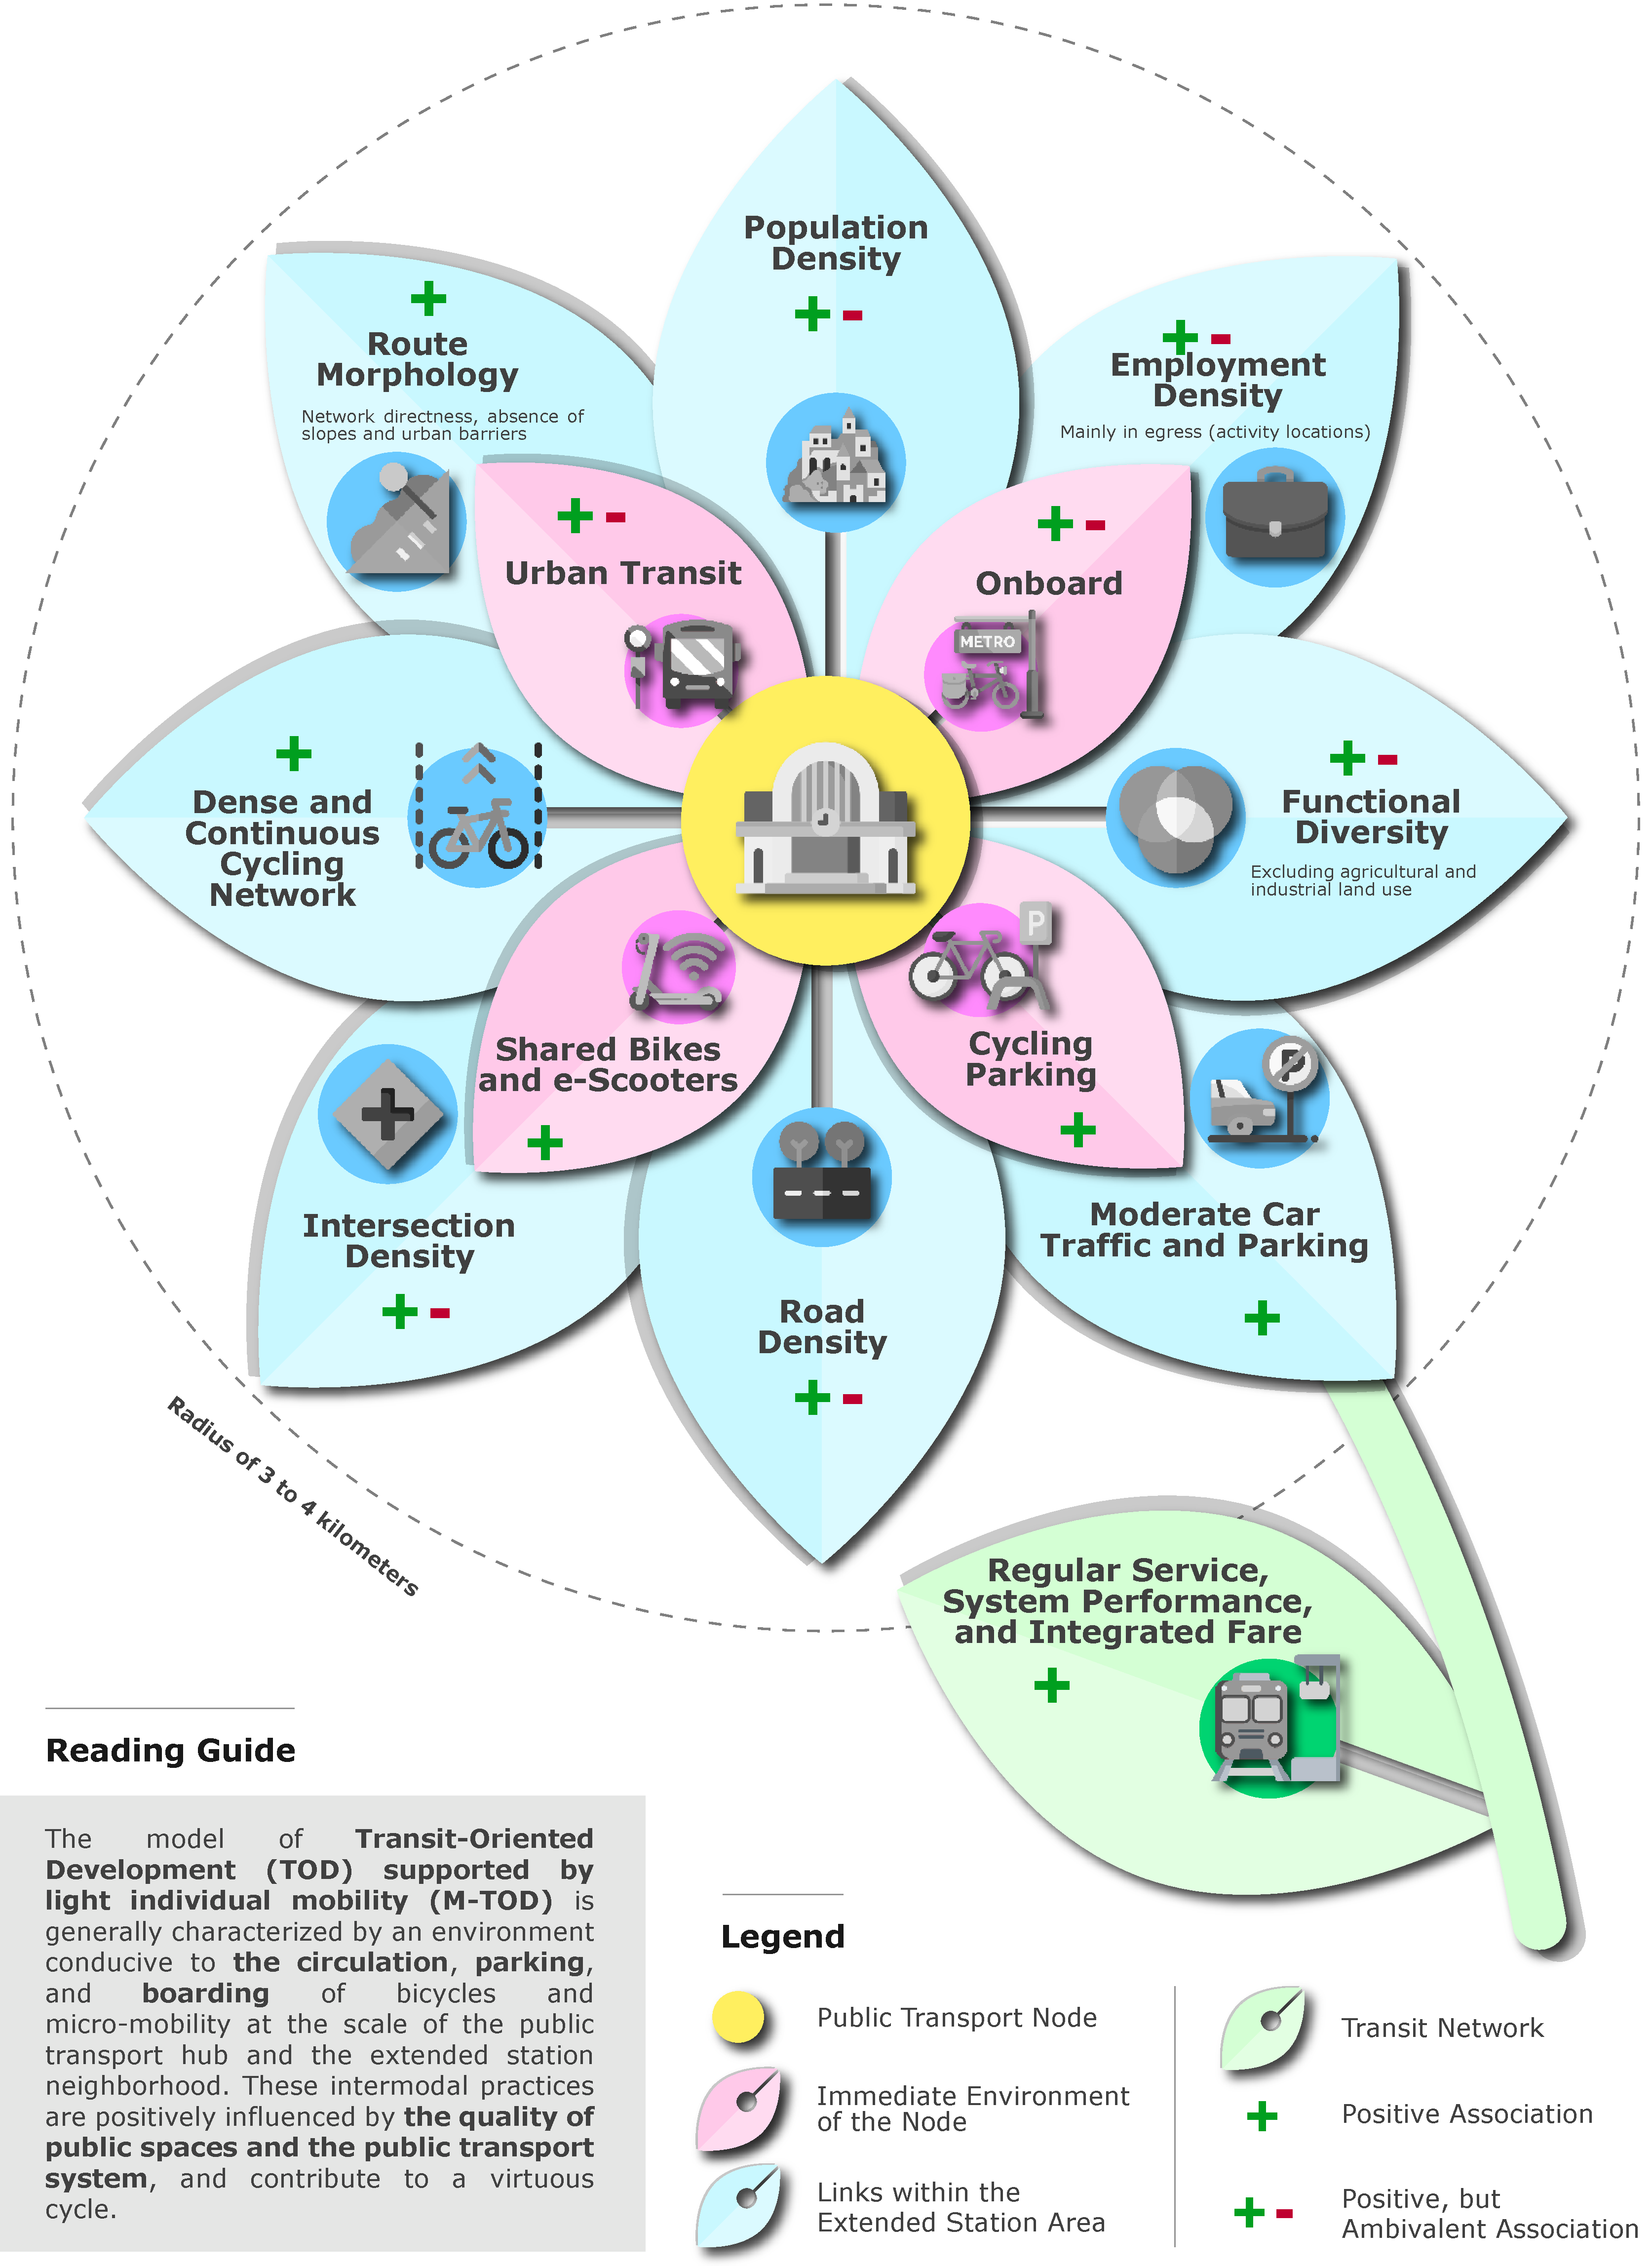
\includegraphics[width=1\columnwidth]{src/Figures/Chap-2/EN_RSL_Fleur_TOD.pdf}}
    \vspace{5pt}
    \begin{flushright}\scriptsize{
    Author: \textcolor{blue}{Dylan Moinse (2023)}
    }\end{flushright}
\end{figure}

% Objectifs
In response to the research questions posed in the \hyperref[chap2:formulation-questions-recherche]{Subsection~\ref{chap2:formulation-questions-recherche}} (page~\pageref{chap2:formulation-questions-recherche}), the goal of this \acrshort{SLR} lies in the ambition to deepen and expand the understanding of knowledge related to \acrshort{M-TOD}. This work aimed to clearly identify the factors that facilitate or hinder the adoption of this urban planning model. In this perspective, the analysis developed in this chapter was based on a set of six research questions, which served as the guiding framework for our study. These questions focus on the interaction between urban dynamics, public policies, and their role in integrating individual light mobility into public transport systems, as well as the influence of these practices on territorial configurations. The detailed examination of the literature highlighted the crucial importance of the \acrshort{7Ds} and mobility behaviors, offering a more nuanced and detailed perspective on these movements and their beneficial implications in the development of an urban model that promotes a sustainable and viable mobility and urban system. This study revealed that the extended influence area of train stations provides accessibility gains to a greater number of potential travelers. As a result, we can refer to the notion of \Commas{territorial reception potential} \textcolor{blue}{\autocite[86]{kaufmann_retour_2014}}\index{Kaufmann, Vincent|pagebf} as a key driver, supported by these mobility practices, linked to the principles of \acrshort{TOD}. In conclusion, the final research question addresses the challenges faced by this emerging urban model, particularly questioning the current gaps in the scientific literature in the face of recent knowledge production related to \acrshort{M-TOD}.%%Translated%%

% 2.*.*.*
\needspace{1\baselineskip} % Reserve space
\subsection*{Gaps in the Scientific Literature
    \label{chap2:literature-gap}
    }

    % Literature gap: state of the literature
As a transition towards the examination of our empirical material, we conclude this chapter by highlighting the main issues that still seem underexplored in relation to the concept of \acrshort{M-TOD}. The bibliometric analysis conducted in the context of our \acrshort{SLR} allowed us to identify various gaps related to the contours of our research topic. First, it is important to note an underrepresentation of studies considering certain forms of individual light mobility. Despite the growing interest in \acrshort{PBS}, \acrshort{DBS}, and \acrshort{DESS} since 2018, studies focusing on scooters and folding bikes, whether electric or non-motorized, remain relatively rare. This observation is accompanied by a focus on urban public transport systems, suggesting an untapped potential in the role of regional rail networks in association with new forms of mobility. Furthermore, we observe that the scientific and technical literature gives little attention to a systemic approach to the entire collective mobility system of a given geographic area, an approach that is crucial for understanding intermodal mobility in a systemic way. Moreover, the current scientific landscape reveals a geographical imbalance, with a predominance of studies set in international or regional agglomerations in China, the United States, and the Netherlands. Finally, the examination of the geographical frameworks studied shows a marked tendency to favor intercommunal and communal scales, while research adopting a regional scale remains exceptional.%%Translated%%

% Literature gap: concepts and methods
In light of the defined theoretical frameworks, we identified an interesting disparity between the frequent mention and use of the \acrshort{TOD} concept in the scientific literature and its near absence under the term \acrshort{M-TOD}. Regarding the research methods employed, we note a majority of studies relying on open or private databases derived from \textsl{Open Data} and \textsl{Big Data}. Furthermore, survey techniques such as questionnaires, interviews, or observations, which are generally more suited to medium-sized areas, are nonetheless equally present depending on the geographical contexts, particularly in Europe. However, it is worth noting the insufficiency of qualitative approaches and, more broadly, mixed methods research, especially concerning emerging individual light mobility options. The analysis methods suggest a strong inclination towards the use of modeling and descriptive statistics as well as \acrshort{GIS}.%%Translated%%

% Literature gap: results
The detailed analysis of the corpus constructed for this \acrshort{SLR} revealed not only disparities in the use of the \acrshort{7Ds} in connection with the \acrshort{M-TOD}, but also led to the development of new questions arising from the confrontation of empirical studies:
    \begin{customitemize}
\item What is the direct or indirect impact of population density on territorial configurations and the mobility practices favored by the \acrshort{M-TOD} urban model?
\item Is the notion of social mix complementary to the principles promoted by the \acrshort{M-TOD}?
\item Do the different forms of modal combinations induce specific needs in terms of infrastructure and cycling facilities?
\item What are the accessibility gains offered by the integration of individual light mobility within public transport systems?
\item How does the influence area of transport nodes vary according to the nature of modal combinations, the different stages of intermodal travel, and environmental and socio-demographic factors?
\item To what extent do the performance of public transport networks and the management of space dedicated to automobiles contribute to a better articulation between urban forms and mobility behaviors?
\item Can the \acrshort{M-TOD} be considered as a factor exacerbating mobility access inequalities?
\item Can this urban model integrate mobility related to leisure, social encounters, or walks (\textsl{undirected travel})?
\item Can the democratization of adopting individual light mobility in intermodality form a virtuous circle influencing urban forms, which, in turn, shape mobility behaviors?
    \end{customitemize}%%Translated%%

% Issues
In light of the challenges raised by the scientific literature regarding the design of an urban system oriented towards the development of public transport networks hybridized with the integration of individual light mobility, the doctoral thesis aims to better understand the key concepts of the \acrshort{M-TOD}. This chapter has highlighted the need to expand the research field on this topic to include a greater variety of mobility forms and levels of geographical analysis, in order to enrich our understanding of this urban planning strategy, reinterpreted through the lens of individual light mobility. These observations lead us to reflect on adopting a geostatistical approach combined with a qualitative methodology, which could provide more nuanced perspectives on individuals' mobility behaviors and experiences.%%Translated%%

% Thesis Structure
In this perspective, our doctoral research revolves around the exploration of a European geographic space at a regional scale, with particular focus on the entire mobility network, primarily structured around railway networks. The next \hyperref[chap3:titre]{chapter} (page~\pageref{chap3:titre}) will be dedicated to defining the geographic scope of the study and presenting our methodology, which includes a field survey. The goal of this mixed-method approach is to capture the development of intermodal practices that combine the use of public transport and emerging forms of individual light mobility, and to examine them in terms of mobility behaviors and their interactions with the urban environment (see \hyperref[chap4:titre]{Chapter~4}, page~\pageref{chap4:titre}). Identifying a social group of cycling commuters actively present in the various territories under study will allow us to explore their interactions in the context of expanded train station neighborhoods, using the concept of intermodal accessibility (see \hyperref[chap5:titre]{Chapter~5}, page~\pageref{chap5:titre}). This geographical approach to distances will lead us to propose a model based on a Node-Place Index, aimed at assessing the potential for urban development in synergy with an alternative mobility system at the regional scale, as outlined in \hyperref[chap6:titre]{Chapter~6} (page~\pageref{chap6:titre}).%%Translated%%

% ___________________________________________
     \newpage
     
% Valorisation scientifique
    \begin{tcolorbox}[colback=white!5!white,
                      colframe=blue!75!blue,
                      title=Valorization
                      \\
                      Chapitre~2]
\Large{\textbf{\textcolor{blue}{Book Chapter:}}}
    \\\\
\small{\textcolor{blue}{\textcite{moinse_systematic_2023}}\index{Moinse, Dylan|pagebf}. \foreignlanguage{english}{\textsl{A Systematic Literature Review on Station Area Integrating Micromobility in Europe: A 21\textsuperscript{st} Century Transit-Oriented Development}}. In: Belaïd,~F., Arora,~A. (eds) \textsl{Smart Cities. Studies in Energy, Resource and Environmental Economics}. Springer, Cham. ISBN: 978-3-031-35663-6 (p.~171-204).
\\
\footnotesize{\url{https://doi.org/10.1007/978-3-031-35664-3_12}} (\textbf{OS})}
    \end{tcolorbox}

    % ___________________________________________
    % Subbibliography
    \newpage
    \sectionheader{Bibliography of Chapter~2}
    \begingroup
    \renewcommand{\bibfont}{\scriptsize}
\printbibliography[segment=\therefsegment, heading=subbibintoc, title={Bibliography of Chapter~2}, label=chap2:bibliographie]
    \endgroup
    \end{refsegment}

%% ______________________________ %%
% CHAPTER 3
%------------------------------%
%% ✎ Dylan (V1) %%%%%%%%% ✅ %%
%% ✎ Alain (V2) %%%%%%%%% ✅ %%
%% ✎ Dylan (V3) %%%%%%%%% ✅ %%
%------------------------------%

%%%%%%%%%%%%%%%%%%%%%%%%%%%%%%%%
% chapter~3
\chapterheader{Doctoral Research Methodology}
\chapter
{A \Commas{Tailor-Made} Survey in the Hauts-de-France Region
    \label{chap3:titre}
    }
    \begin{refsegment}

    % Arrière-plan chapitre~3
    \AddToShipoutPictureBG*{%
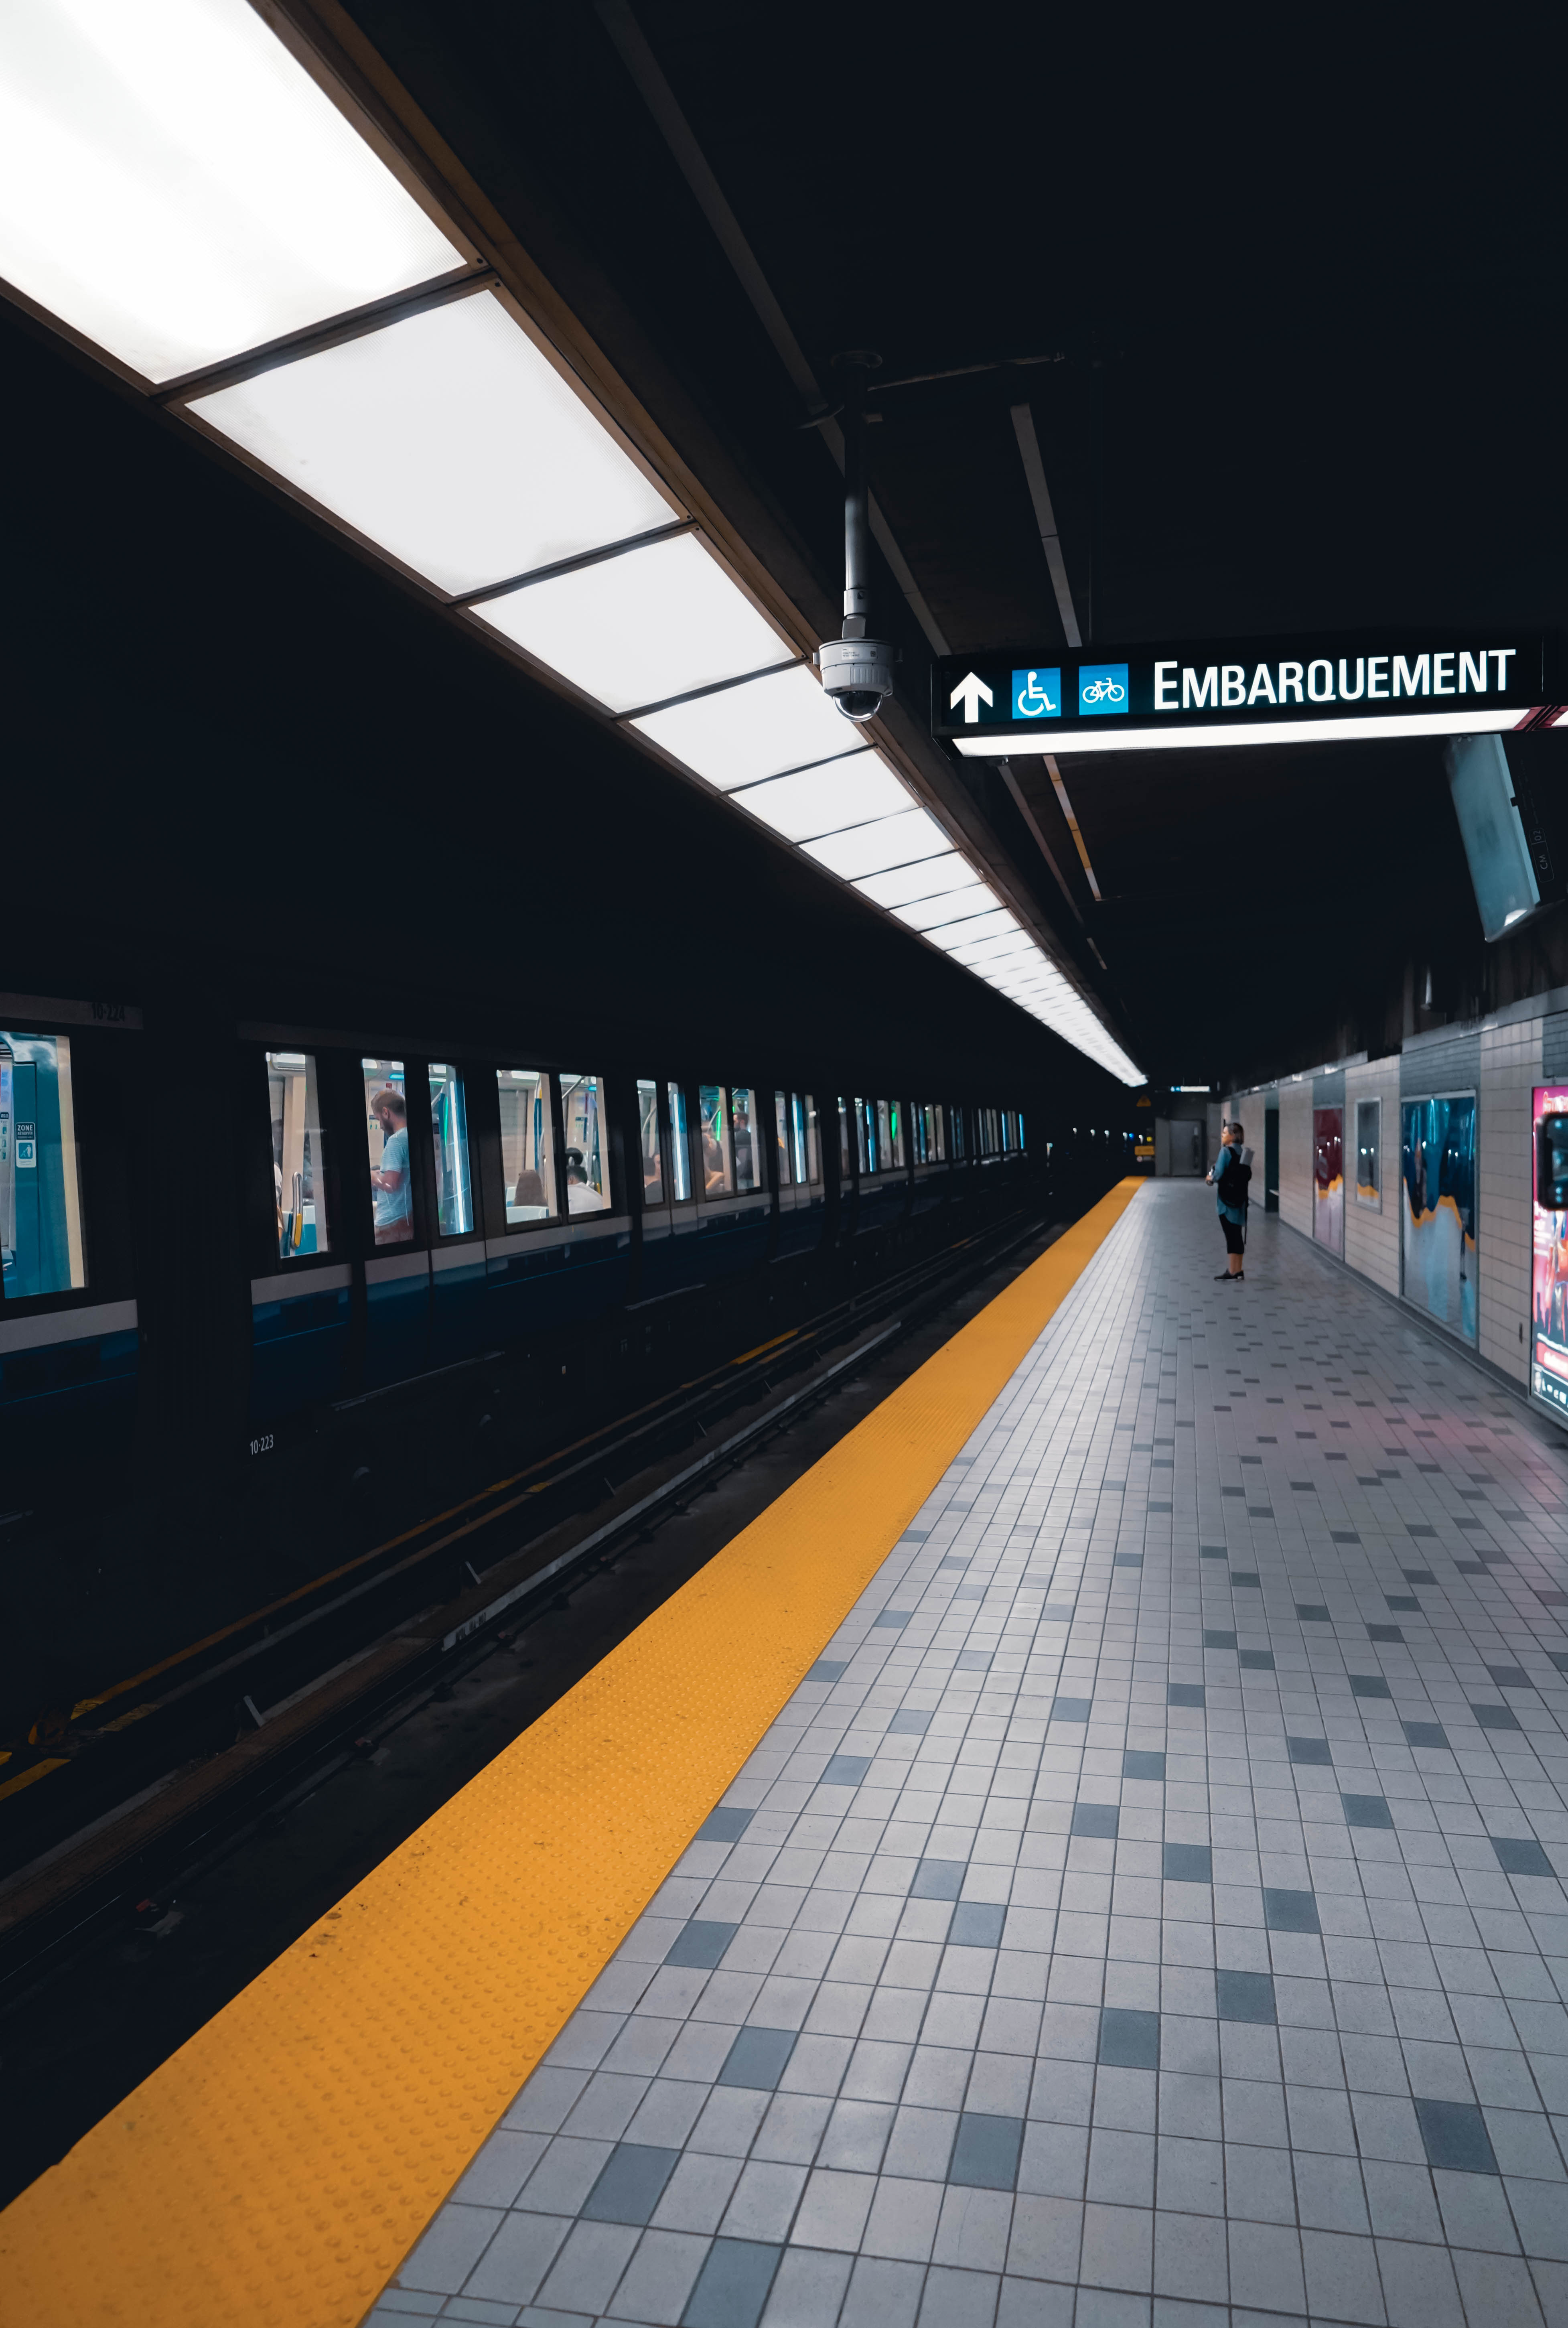
\includegraphics[width=\paperwidth,height=\paperheight]{src/Figures/Arriere_plan/Arriere_plan_Chap_3.jpg}
    }

% Rectangle
\AddToShipoutPictureBG*{
  \begin{tikzpicture}[remember picture,overlay]
    \node[fill=white, opacity=0.75, text width=\paperwidth, minimum height=7cm, anchor=north] 
    at ([yshift=-2cm]current page.north) {};
  \end{tikzpicture}
}

% Source
\AddToShipoutPictureFG*{
  \AtPageLowerRight{
    \raisebox{1cm}{
      \hspace{16cm}
      
\begin{tikzpicture}
        \node[fill=white, rounded corners=5pt, inner sep=5pt, align=center] {
          \tiny{Photography: \textcolor{blue}{Dylan Moinse (2022)}}
        };
      \end{tikzpicture}
    }
  }
}

    % ___________________________________________
    % Mini Table of Contents
    \cleardoublepage
    \setcounter{tocdepth}{2}
    % Redefine local table of contents title
    \renewcommand{\localcontentsname}{Table of Contents for Chapter~3}
\localtableofcontents

% Réinitialiser numérotation section
\setcounter{section}{0}

    % ___________________________________________
    % Graphical abstract
    \newpage
\section*{Key Points of Chapter~3
    \label{chap3:graphical-abstract}
    }
    \markright{Chapter Preambule}{}

% \begin{figure}[h!]\vspace*{4pt}
%         \caption*{}
%         \label{graphical-abstract-chap3}
%         \centerline{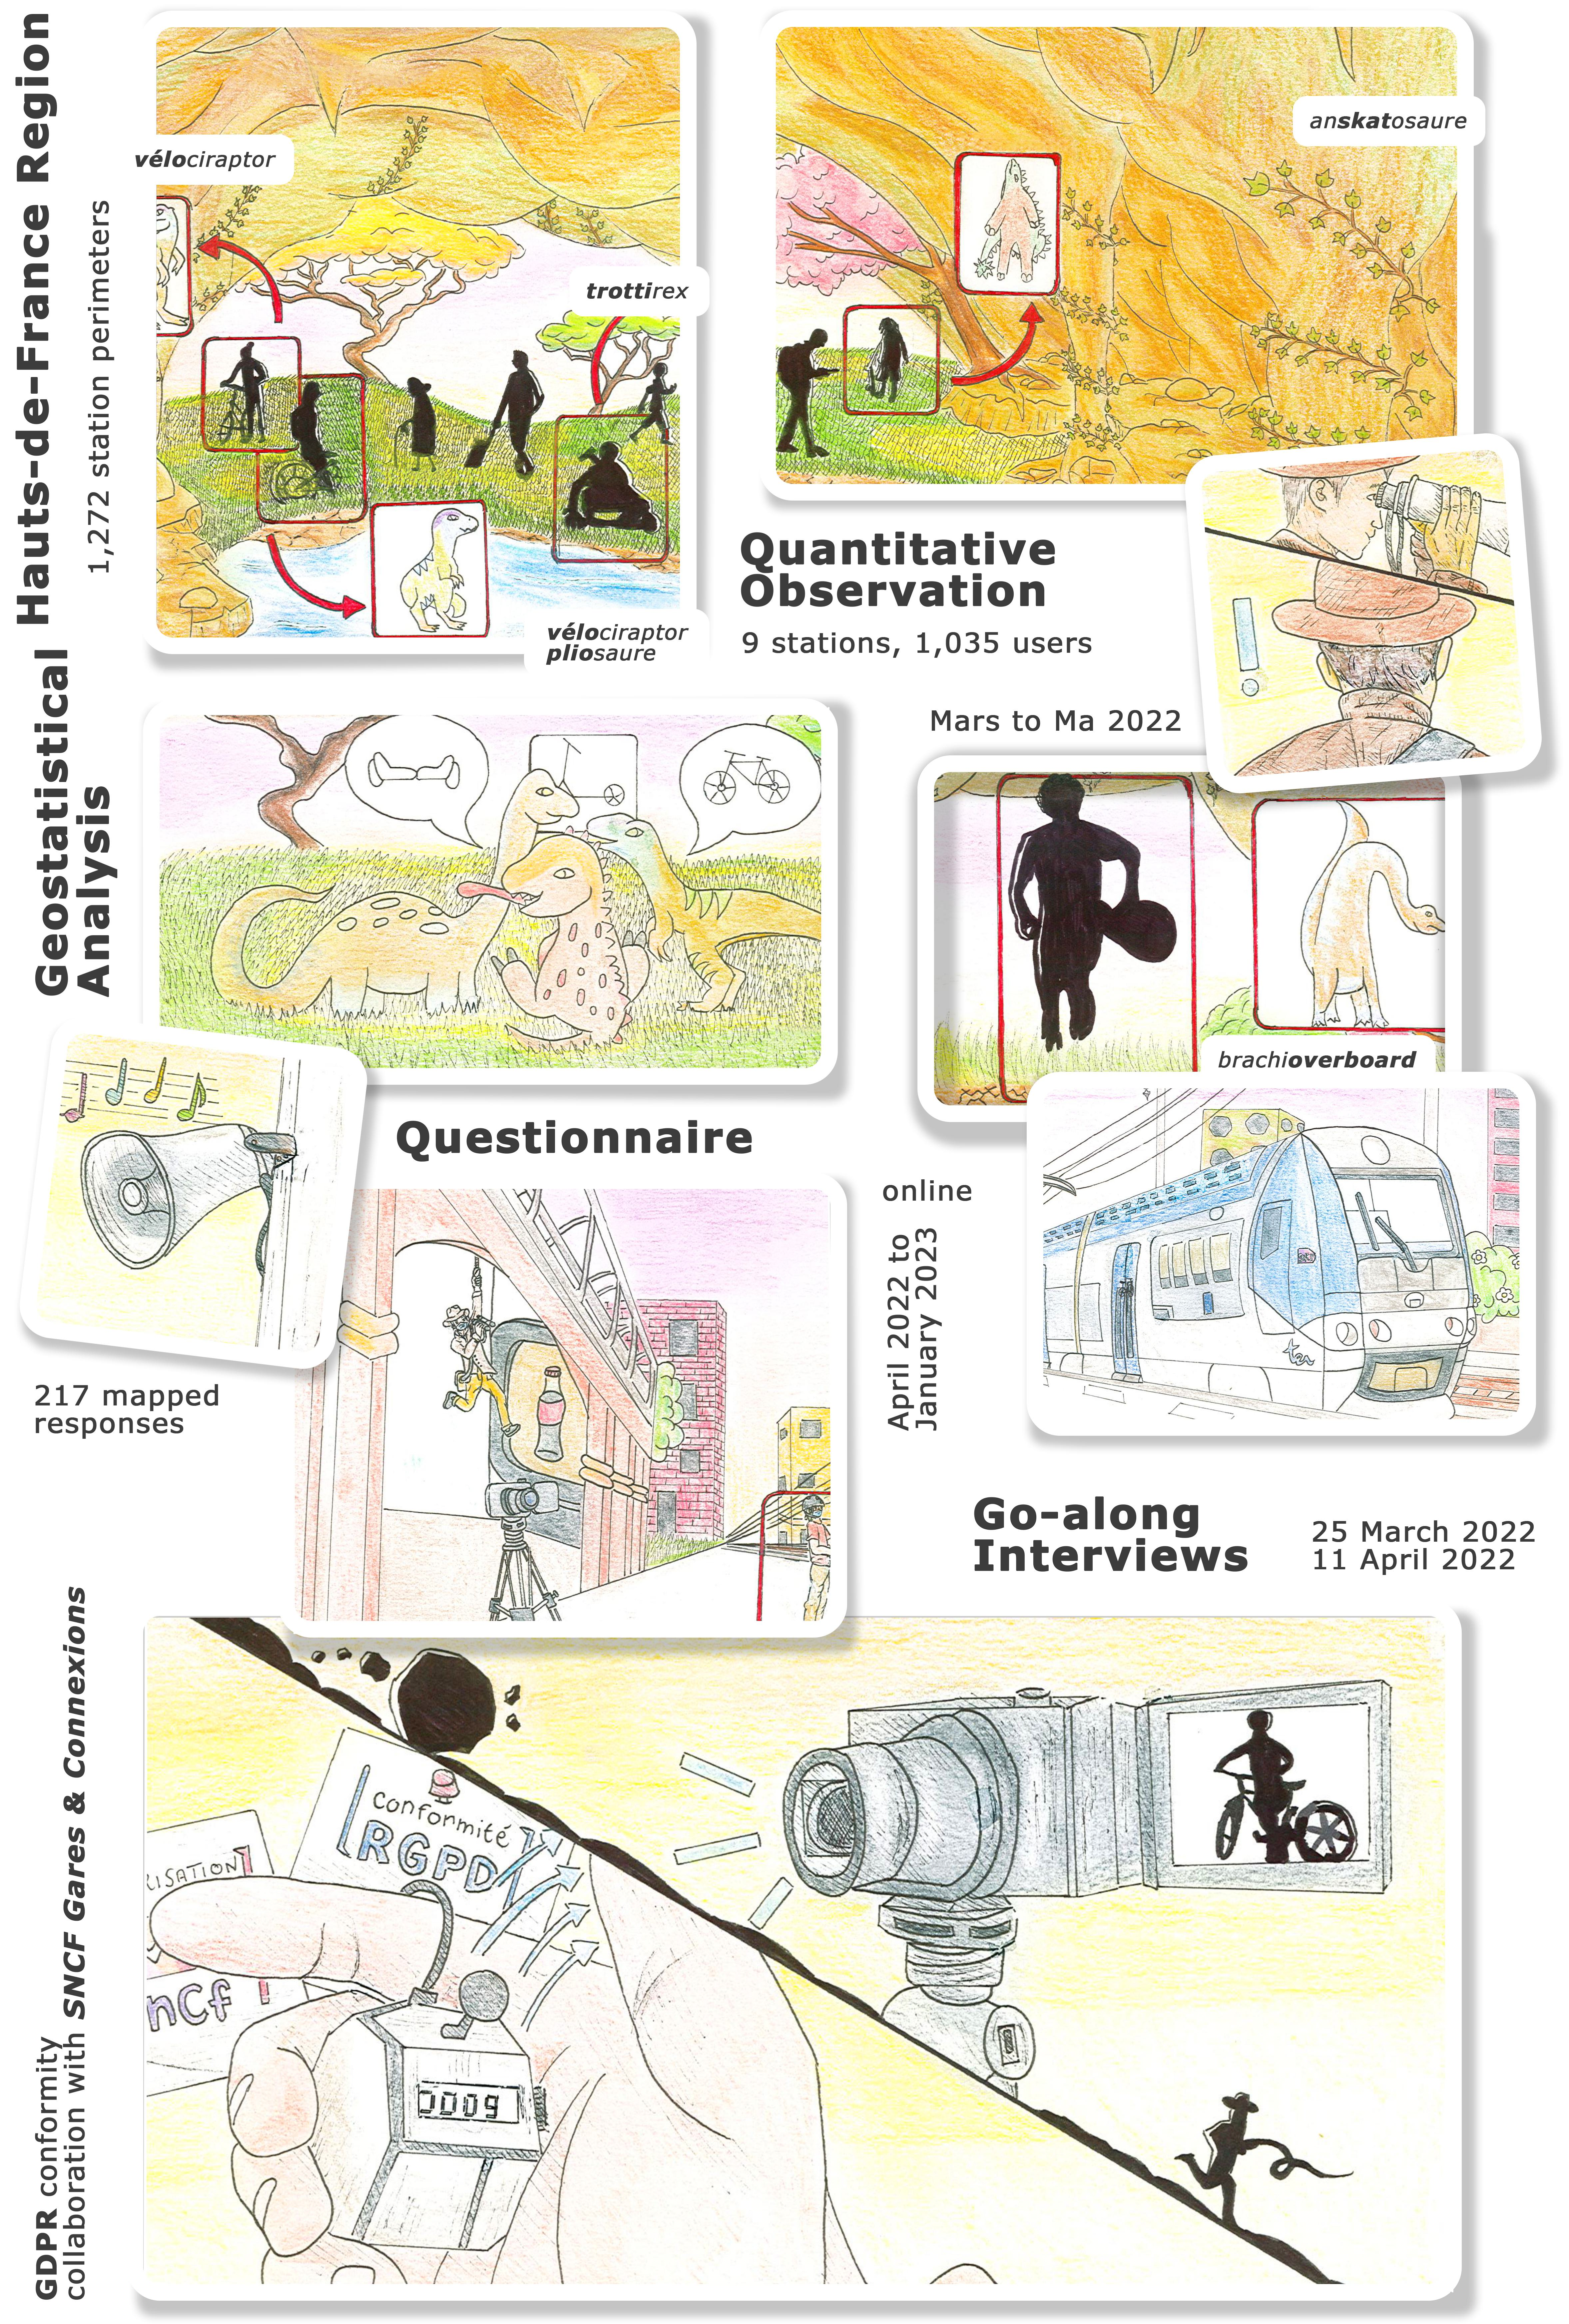
\includegraphics[width=1\columnwidth]{src/Figures/Graphical-abstract/EN_Graphical_abstract_chap3.jpg}}
%         \vspace{5pt}
%         \begin{flushright}\scriptsize{
%         Source: \textcolor{blue}{Morgan Moinse (2022)}
%         }\end{flushright}
%     \end{figure}

    % ___________________________________________
    % Preamble
    \newpage
    \begin{tcolorbox}[colback=white!5!white,
                      colframe=blue!75!blue,
                      title=
                      \bigskip
                      \center{\textbf{Preamble of Chapter~3}}
                      \\
                      \raggedright{\small{Chapter composed of \pagedifference{chap3:titre}{part1:conclusion} pages, including \pagedifference{chap3:bibliographie}{part1:conclusion} pages of bibliography}}
                      \bigskip]
\Large{\textcolor{blue}{\textbf{Abstract:}}}
    \\
    \small{
This chapter presents the methodology developed to investigate intermodal practices in the train station districts of the Hauts-de-France region. Starting with a contextualization of our case study alongside the description of our mixed research methods, we sought to design a methodology based on a multidimensional and multiscalar approach. Structured into five sections, this chapter successively addresses the definition of the geographical scope, the spatial projection of train station districts, and the implementation of a survey combining quantitative observation, questionnaire administration, and guided tours.%%Translated%%
    \\
The first section defines the geographical boundaries of the study and justifies the choice of the Hauts-de-France region as the analytical framework (see \hyperref[chap3:region-hauts-de-france]{Section~1}, page~\pageref{chap3:region-hauts-de-france}). This choice is based on its dense rail network and its \textsl{a priori} polycentric structure, even though it faces major mobility challenges. Particular attention is given to the reflective stance of the researcher and to ethical considerations.%%Translated%%
    \\
Train station districts are defined as spatial units theoretically accessible on foot or with the use of light individual mobility (see \hyperref[chap3:quartiers-gare]{Section~2}, page~\pageref{chap3:quartiers-gare}). A specific approach, integrating spatial criteria such as acceptable distances and urban environment characteristics, is used to define and map these areas of influence. This approach allows for examining the spatial and functional configuration of these strategic spaces using geostatistical tools.%%Translated%%
    \\
The third section focuses on the quantitative observation of passengers at train stations, particularly users of light individual mobility, who are often underrepresented in public surveys (see \hyperref[chap3:observation-quantitative]{Section~3}, page~\pageref{chap3:observation-quantitative}). The methodological protocol, combining counting and ethnographic observation, is detailed through observation grids applied in nine selected stations.%%Translated%%
    \\
The fourth section discusses the design and administration of a questionnaire targeted at intermodal passengers (see \hyperref[chap3:questionnaire]{Section~4}, page~\pageref{chap3:questionnaire}). It highlights the usefulness of this tool for collecting data on travel practices, perceptions, and expressed needs. The structure of the questionnaire, sampling steps, and response validation are detailed, facilitating the linking of declared movements with geostatistical and behavioral analyses.%%Translated%%
    \\
Finally, the fifth section introduces the approach of guided tours, a qualitative method conducted \textsl{in situ}, allowing for the exploration of user experiences in motion (see \hyperref[chap3:parcours-commente]{Section~5}, page~\pageref{chap3:parcours-commente}). It aims to deepen the understanding of modal choice mechanisms and infrastructure use from the perspective of micro-geographical reports.%%Translated%%
    }
    \tcblower
\Large{\textcolor{blue}{\textbf{Keywords:}}}
    \\
    \small{
Geostatistical analysis;
Hauts-de-France;
Mixed methods;
Quantitative observation;
Research field;
Guided tours;
Questionnaire;
Train station districts
    }
    \end{tcolorbox}

    % ___________________________________________
    % 3.*.
    \newpage
    \needspace{1\baselineskip} % Reserve space
    \addcontentsline{toc}{section}{Introduction of Chapter~3}
    \sectionheader{Introduction of Chapter~3}
\section*{Introduction of Chapter~3
    \label{chap3:introduction}
    }
    \markright{Introduction of Chapter~3}{} 

    % Citation
\begin{displayquote}
\Commas{[\dots] \textsl{through creative processes (ad hoc methods) or synergies (between existing methods), we are able to refine the quality of observation, and then analysis, depending on the case, of a category of daily mobility behaviors or the range of uses of a transport network. The contributions reflect researchers' interest in mobility issues and the great creativity they demonstrate in capturing it.} [\dots] \textsl{To understand this, the analogy with the microscope seems quite telling. Depending on the focal length chosen, the image that a laboratory worker sees forming in the microscope is different each time. However, they are always observing the same reality, but at different scales or, more precisely, from a different perspective. Neither of the images obtained is more true than the other, but they provide a different view of reality.} [\dots] \textsl{Although the complementarity of quantitative and qualitative research is often praised as an ideal, few researchers have actually practiced it to date.} [\dots] \textsl{Methodological innovations and hybridizations are closely linked to the question of researchers' professional practices. Many articles explicitly reference this. These innovations and hybridizations are most often carried out in teams, where each person brings their own practices, skills, and methodological or disciplinary expertise. This collective work, reflected in the contributions gathered here, most of which are written by multiple authors, requires time and coordination to share and implement these know-how within an operational framework. It also requires audacity and creativity to explore experimentation, as well as enough trust, and humility, to (re)acknowledge the values and limits of each method. Finally, it calls for the ability to adapt, to question oneself in response to multiple stimuli from other scientific approaches, different professional viewpoints, or innovations arising from practical uses. Methodological innovations and hybridizations thus appear as a reflection of human creativity, societal progress, and territorial development. It is certainly within this creative and highly collaborative work that the scientific innovations of tomorrow will emerge.}}\footnote{~
    \Commas{[\dots] \textsl{par des processus créatifs (méthodes ad hoc) ou des synergies (entre méthodes déjà existantes), on parvient à affiner la qualité de l’observation, puis de l’analyse, selon le cas, d’une catégorie de comportements de déplacement quotidien ou de l’éventail des usages d’un réseau de transport. Les contributions témoignent de l’intérêt des chercheurs pour les questions de mobilité et de la grande créativité dont ils font preuve pour la saisir.} [\dots] \textsl{Pour le comprendre, l’analogie avec le microscope paraît assez parlante. Selon la focale qu’il choisit, l’image qu’un laborantin voit se former dans le microscope est à chaque fois différente. Il observe pourtant toujours la même réalité, mais à des échelles différentes ou, plus exactement, d’un point de vue différent. Ni l’une ni l’autre des images obtenues n’est plus vraie qu’une autre, mais elles rendent compte d’un regard différent sur la réalité.} [\dots] \textsl{Si la complémentarité des travaux de recherche quantitatifs et qualitatifs est louée de manière récurrente tel un idéal incantatoire, jusqu’à ce jour, peu de chercheurs la pratiquaient dans les faits.} [\dots] \textsl{Les innovations et hybridations méthodologiques renvoient de manière assez directe à la question des pratiques professionnelles des chercheurs. Nombreux sont, du reste, les articles à y faire référence explicitement. Ces innovations et hybridations sont le plus souvent réalisées en équipe, dans lesquelles chacune et chacun apporte ses pratiques, ses savoir-faire et ses compétences méthodologiques ou disciplinaires. Ce travail collectif, qui se reflète dans les contributions rassemblées ici, écrites pour la plupart par plusieurs auteurs, nécessite du temps et de la coordination pour partager les savoir-faire et les mettre en œuvre autour d’un dispositif opérationnalisable. Il nécessite également de l’audace et de la créativité pour pousser la porte de l’expérimentation et suffisamment de confiance, mais aussi d’humilité pour (re)connaître les valeurs et les limites de chaque méthode. Enfin, il suppose une capacité d’adaptation, de remise en question sous l’effet de stimulations multiples venues d’autres approches scientifiques, d’autres points de vue professionnels ou encore d’autres innovations venues des usages. Les innovations et hybridations méthodologiques apparaissent alors comme le reflet des capacités créatives des hommes, de leurs sociétés et de leurs territoires. C’est certainement dans ce travail créatif et fortement collaboratif que se nichent les innovations scientifiques de demain.}} \textcolor{blue}{\autocite[12-14, 160]{meissonnier_connaissance_2020}}\index{Meissonnier, Joël|pagebf}\index{Vincent, Stéphanie|pagebf}\index{Rabaud, Mathieu|pagebf}\index{Kaufmann, Vincent|pagebf}
}

\textcolor{blue}{Joël} \textcolor{blue}{\textcite[12-14, 160]{meissonnier_connaissance_2020}}\index{Meissonnier, Joël|pagebf}\index{Vincent, Stéphanie|pagebf}\index{Rabaud, Mathieu|pagebf}\index{Kaufmann, Vincent|pagebf}. \textsl{Connaissance des mobilités: hybridation des méthodes, diversification des sources}, Éditions du Cerema, Lyon, 176~p. ISBN: \href{https://search.worldcat.org/fr/title/1236011015}{978-2-37180-423-4}
    \end{displayquote}

    % Introduction
\lettrine[lines=3, findent=8pt, nindent=0pt]{\lettrinefont S}{tructuring} of our study is based on the observation of practices and the explanation of intermodal behaviors, with a territorial approach focused on the train station and its surroundings, understood as the interaction of environmental, social, and built dimensions within a single urban system, referencing the concept of \Commas{station interconnection} \textcolor{blue}{\autocite[7]{moretti_interconnexion_1999}}\index{Moretti, Anna|pagebf}\index{Vacheret, Guy|pagebf}. To achieve this, our methodology for studying the stations, their environment, and the practices that unfold within them emphasizes a multidimensional and multiscalar approach. This relational approach articulates three levels of observation: (i) a relational logic, focused on the connection function of network nodes, (ii) a territorial logic, addressing human activities in polarized locations, and (iii) a usage logic, linking space to the behaviors of populations frequenting these nodes \textcolor{blue}{\autocites[9]{moretti_interconnexion_1999}[210-212]{menerault_gares_2001}}\index{Menerault, Philippe|pagebf}\index{Barré, Alain|pagebf}\index{Moretti, Anna|pagebf}\index{Vacheret, Guy|pagebf}. Our ambition is thus to capture the \Commas{territorial accessibility system} in its complexity, by integrating \gls{accessibility} \textsl{of} the territory and \textsl{to} the territory, defined respectively as spatial and social potential, and the interactions between these two dimensions, structured by the geographical space configuration and the characteristics of social groups \textcolor{blue}{\autocite[6]{richer_mesurer_2012}}\index{Richer, Cyprien|pagebf}\index{Palmier, Patrick|pagebf}. We have then leveraged the strengths of both quantitative and qualitative approaches to design an integrated methodological framework \textcolor{blue}{\autocite[]{bergman_advances_2008}}\index{Richer, Cyprien|pagebf}.%%Translated%%

    % Mixed Methods
Rather than opposing them, methods for analyzing movements, whether quantitative or qualitative, would benefit from being considered in a complementary logic \textcolor{blue}{\autocite[6]{klein_mobilites_2007}}\index{Klein, Olivier|pagebf}\index{Ortar, Nathalie|pagebf}\index{Pochet, Pascal|pagebf}. Such an approach implies a more disciplinary sharing focused on the objects of study. In this regard, \textcolor{blue}{\textcite[4]{higgins_forty_2016}}\index{Higgins, Christopher~D.|pagebf}\index{Kanaroglou, Pavlos~S.|pagebf} emphasize the value of combining \Commas{normative} approaches, which qualify the types of \acrshort{TOD}, with \Commas{positive} systematic approaches. It is in this context that the use of various methodological techniques we have implemented is justified, including the exploitation of existing databases combined with observation sessions, questionnaires, and field interviews \textsl{in situ} \textcolor{blue}{\autocite[128]{dureau_lobservation_2014}}\index{Dureau, Françoise|pagebf}\index{Giroud, Matthieu|pagebf}\index{Lévy, Jean-Pierre|pagebf}. The objective of these mixed methods, from a conceptual point of view, is to provide an exploratory basis from \textsl{action captured} through observation. This step allows for the design and adjustment of a questionnaire collecting what is \textsl{signified}. Reported responses are then examined through interviews that capture the experience as it is \textsl{lived and perceived} \textcolor{blue}{\autocite[215]{paugam_enquete_2012}}\index{Paugam, Serge|pagebf}.%%Translated%%

    % Methods Description
The combination of a \Commas{custom} survey, integrating quantitative observation, a questionnaire, and go-along interviews for cycling travelers, aims to provide a comprehensive perspective on a topic that is still under-documented by empirical data (for reference, see \hyperref[fig-introduction:methodes-hypotheses]{Figure~\ref{fig-introduction:methodes-hypotheses}}, in the \hyperref[introduction-generale:methodologie]{general introduction}, page~\pageref{fig-introduction:methodes-hypotheses}). \textcolor{blue}{Joël} \textcolor{blue}{\textcite[24]{meissonnier_pour_2012}}\index{Meissonnier, Joël|pagebf}, as well as \textcolor{blue}{Karel} \textcolor{blue}{\textcite[291]{martens_bicycle_2004}}\index{Martens, Karel|pagebf} for the combined use of \gls{bicycle} and public transport, emphasize the importance of recognizing the limitations of traditional quantitative surveys, such as the \acrfull{PMD}, when it comes to capturing the dynamics of daily mobility, and even more so the chains of movement \textcolor{blue}{\autocite[10]{kieffer_chainage_2011}}\index{Kieffer, Lionel|pagebf}\index{Oliveau, Sébastien|pagebf}\index{Audard, Frédéric|pagebf}. This requires reconsidering the approach by enriching existing databases with field surveys tailored to the demands of our research question. This approach draws on pre-existing work that has paved the way and inspired our methodology. For example, \textcolor{blue}{François de} \textcolor{blue}{\textcite[42]{singly_questionnaire_2016}}\index{Singly, François de|pagebf} highlights the value, in social sciences, of combining the questionnaire, which makes visible the social determinants of trajectories, with interviews, which shed light on the individual construction process of these trajectories. Thus, several studies have demonstrated the value of employing a mixed methodology that combines direct observation, questionnaires, and \Commas{mobile} interviews \textcolor{blue}{\autocites[258]{greene_toward_1989}[120]{bergeron_uncovering_2014}[3]{despres_replacer_2019}}\index{Greene, Jennifer~C.|pagebf}\index{Caracelli, Valerie~J.|pagebf}\index{Graham, Wendy~F.|pagebf}\index{Bergeron, Julie|pagebf}\index{Paquette, Sylvain|pagebf}\index{Poullaouec-Gonidec, Philippe|pagebf}\index{Desprès, Michel|pagebf}\index{Lord, Sébastien|pagebf}\index{Negron-Poblete, Paula|pagebf}.%%Translated%%

    % Outline Announcement 1
The first part of this chapter focuses on defining the geographical area, considered from a macroscopic perspective (\hyperref[chap3:region-hauts-de-france]{Section~1}, page~\pageref{chap3:region-hauts-de-france}). This approach aims to justify the relevance of a regional perspective by presenting the mobility issues as well as the strategic documents established by the competent administrative authority (\hyperref[chap3:regard-privilegie-region-hdf]{Subsection~1.1}, page~\pageref{chap3:regard-privilegie-region-hdf}). In the second part, a sociological self-analysis exercise will be conducted to objectify our positioning in relation to the field, understood both as the subject of research and the geographical context (\hyperref[chap3:auto-analyse-sociologique]{Subsection~1.2}, page~\pageref{chap3:auto-analyse-sociologique}). The description of the geographical scope in which our empirical material is situated will conclude with our relationship to the main mobility manager and the alignment of our survey methods with the principles of research ethics (\hyperref[chap3:preparation-terrain-geographique]{Subsection~1.3}, page~\pageref{chap3:preparation-terrain-geographique}).%%Translated%%

    % Outline Announcement 2
Once the geographical framework is introduced, we will focus on detailing the process of spatializing the train station neighborhoods, understood as spatial units accessible on foot and by light individual mobility, from a microscopic perspective (\hyperref[chap3:quartiers-gare]{Section~2}, page~\pageref{chap3:quartiers-gare}). We will define the methodological rules for mapping these influence areas, based on the distances deemed acceptable and the typology of the stations, as determined through our field survey (\hyperref[chap3:quartiers-gare-distances]{Subsection~2.1}, page~\pageref{chap3:quartiers-gare-distances}). Once the sizes of the station neighborhoods are defined, our attention will shift to their shapes and boundaries, influenced by the characteristics of the built environment. This step will include a reflection on the methods used to generate and represent these shapes (\hyperref[chap3:quartiers-gare-formes]{Subsection~2.2}, page~\pageref{chap3:quartiers-gare-formes}). To conclude this section, we will present the principles for extracting and processing the geostatistical data we have set for ourselves. We will outline the criteria used to exploit the databases, aiming to achieve a high degree of resolution in geographic information (\hyperref[chap3:quartiers-gare-analyse-geostatistique]{Subsection~2.3}, page~\pageref{chap3:quartiers-gare-analyse-geostatistique}).%%Translated%%

    % Outline Announcement 3
The third section of our methodological chapter will be dedicated to describing the quantitative observation approach for cycling travelers, with the aim of providing an overall overview and evaluating current trends, which are still under-documented (\hyperref[chap3:observation-quantitative]{Section~3}, page~\pageref{chap3:observation-quantitative}). First, we will define what constitutes quantitative observation, explaining its relevance to some of our research objectives (\hyperref[chap3:observation-quantitative-outil-adapte]{Subsection~3.1}, page~\pageref{chap3:observation-quantitative-outil-adapte}). Then, we will detail the methodological protocol of our approach, combining counting and ethnographic observation. We will present the observation grid used and the methods for its implementation (\hyperref[chap3:methodologie-observation-quantitative]{Subsection~3.2}, page~\pageref{chap3:methodologie-observation-quantitative}). The section concludes with the contextualization of the nine stations examined in this survey, where we will justify their selection (\hyperref[chap3:observation-quantitative-gares-examinees]{Subsection~3.3}, page~\pageref{chap3:observation-quantitative-gares-examinees}).%%Translated%%

    % Outline Announcement 4
Following the quantitative observation, we will introduce the questionnaire addressed to users (\hyperref[chap3:questionnaire]{Section~4}, page~\pageref{chap3:questionnaire}). We will emphasize the added value of this methodological tool (\hyperref[chap3:apports-questionnaire-usagers]{Subsection~4.1}, page~\pageref{chap3:apports-questionnaire-usagers}). We will then detail the process of administering the questionnaire, presenting its general structure, the sampling process, and the validation of the responses obtained, which have allowed the declared movements to be projected (\hyperref[chap3:administration-questionnaire-usagers]{Subsection~4.2}, page~\pageref{chap3:administration-questionnaire-usagers}).%%Translated%%

    % Outline Announcement 5
The third approach of our field survey, which will be presented throughout this thesis, is based on an initial exploration of go-along interviews (\hyperref[chap3:parcours-commente]{Section~5}, page~\pageref{chap3:parcours-commente}). First, we will place this in-situ interview method in context, emphasizing its different variations (\hyperref[chap3:parcours-commente-definition]{Subsection~5.1}, page~\pageref{chap3:parcours-commente-definition}). Then, we will show how this method was adapted to our field of study, through the \Commas{micro-geographical} reports generated (\hyperref[chap3:parcours-commente-administration-participants]{Subsection~5.2}, page~\pageref{chap3:parcours-commente-administration-participants}).%%Translated%%

    % Outline Announcement 6
In conclusion, we will place the various approaches within an overarching view, to illustrate their articulation and connection with our research hypotheses (\hyperref[chap3:conclusion]{Chapter~3 conclusion}, page~\pageref{chap3:conclusion}).%%Translated%%

     % ___________________________________________
    % 3.1.
    \newpage
    \needspace{1\baselineskip} % Reserve space
    \sectionheader{Contextualization of the Hauts-de-France Region}
\section{Defining the Geographical Area Bound by the Hauts-de-France Region
    \label{chap3:region-hauts-de-france}
    }

    % Introduction
Entering the field requires first and foremost justifying the choice of this boundary and placing it in its context to understand its local characteristics and territorial challenges. This approach also involves introspection on our own personal and ethical relationship to the places explored and the people interviewed. This first section thus aims to define the geographical framework of our empirical research, while explaining the foundations of our methodological stance. A study from the \acrshort{TOD} perspective reveals its full value when it is part of a regional approach, with the goal of establishing a comprehensive vision for regional development \textcolor{blue}{\autocite[24]{lo_feudo_scenario_2014}}\index{Lo Feudo, Fausto|pagebf}\index{Menerault, Philippe|pagebf}\index{L'Hostis, Alain|pagebf}\index{Festa, Demetrio Carmine|pagebf}. Public transport, and more specifically rail, is a structuring lever for regional planning, perceived in Hauts-de-France as a \Commas{spatial capital offering multiple opportunities} \textcolor{blue}{\autocite[147, 163]{baron_reseaux_2017}}\index{Baron, Nacima|pagebf}\index{Messulam, Pierre|pagebf}. As evidenced by the guidelines defined by \textcolor{blue}{\textcite[17]{region_hauts-de-france_planification_2024}}\index{Région Hauts-de-France@\textsl{Région Hauts-de-France}|pagebf}, which aim to \Commas{\textsl{make the regional transport network the backbone of mobility in Hauts-de-France} [\dots] \textsl{focusing primarily on the regional structuring network (rail and road lines)} [\dots] [with a system of] \textsl{feeders to these modes through relevant alternatives}}.%%Translated%%

% Announcement of the plan
First, we will begin by explaining and describing the situation and challenges of the Hauts-de-France region, which serves as the geographical framework for this research (see the \hyperref[chap3:regard-privilegie-region-hdf]{section on the privileged perspective on the Hauts-de-France region}, page~\pageref{chap3:regard-privilegie-region-hdf}). Through this detailed exploration of the regional territory, we will have the opportunity to establish a scientific objectification stance supported by a method of \Commas{sociological self-analysis} (see the \hyperref[chap3:auto-analyse-sociologique]{section on sociological reflexivity}, page~\pageref{chap3:auto-analyse-sociologique}). We will also address the ethical aspects of our empirical research by describing the actions taken to ensure adherence to these principles in our interactions with local actors and the territories involved (see the \hyperref[chap3:preparation-terrain-geographique]{section on research ethics compliance}, page~\pageref{chap3:preparation-terrain-geographique}).%%Translated%%

% 3.1.1.
\needspace{1\baselineskip} % Reserve space
\subsection{Action Research and Public Policy Territories: A Privileged Perspective on the Hauts-de-France Region
    \label{chap3:regard-privilegie-region-hdf}
    }

    % Introduction
In the French context, and for most geographers, the region is often considered the fundamental territorial unit in the functioning of the globalized economic system \textcolor{blue}{\autocite[]{calthorpe_regional_2001}}\index{Calthorpe, Peter|pagebf}\index{Fulton, William|pagebf}. However, this conception raises an important question: are we referring to an \textsl{urban} or \textsl{functional} region, in terms of daily flows, or a \textsl{political} region, defined by administrative divisions? Situated within the ecological and connected transition program \textsl{rev3} (\textsl{Third Industrial Revolution})\footnote{~
    The 21\textsuperscript{st} century is marked by the \textsl{Third Industrial Revolution}, as referenced in the work by economist \textcolor{blue}{Jeremy} \textcolor{blue}{\textcite[338]{rifkin_troisieme_2012}}\index{Rifkin, Jeremy|pagebf}, one of whose five pillars is the emergence of a digital and electrical economy, partly expressed through the sharing of connected transportation. For the author, the \textsl{Third Industrial Revolution} disrupts traditional ways of thinking about and practicing urban mobility. It is within this framework that the author was consulted to devise a roadmap for the Hauts-de-France region. The acronym \textsl{rev3}, led by the Region and the \acrfull{CCI} Hauts-de-France, refers to this policy in the Hauts-de-France that proposes models for territorial and mobility development toward 2050.
}, the present doctoral project could legitimately focus on the institutional region. However, other arguments support the deliberate choice to concentrate on the administrative region, as developed in the doctoral thesis of \textcolor{blue}{Julia} \textcolor{blue}{\textcite[166]{frotey_acteurs_2021}}\index{Frotey, Julia|pagebf}\index{Deboudt, Philippe|pagebf}\index{Castex, Élodie|pagebf}\index{Frère, Séverine|pagebf} on the development of electromobility in the Hauts-de-France. Historically, geography has sought to distance itself from political divisions in order to better understand the complexity of spatial functioning, considering the flows and exchanges that traverse them \textcolor{blue}{\autocite[]{pumain_regionalisation_2016}}\index{Pumain, Denise|pagebf}. This distancing, particularly prominent after the war—\textcolor{blue}{\textcite[16-18]{menerault_reseaux_1991}}\index{Menerault, Philippe|pagebf}\index{Dupuy, Gabriel|pagebf} referred to it as \Commas{eclipse} in his doctoral work—began to fade in the 1970s, when political geography regained an interest in territories, viewed as forms of spatial organization linked to public action.%%Translated%%

% Regional geography
More broadly, this reflection on the institutional regional scale is part of regional geography. It resonates with the long process of decentralization initiated in France, as well as the recent context of regional mergers. As \textcolor{blue}{Nicole} \textcolor{blue}{\textcite[107]{girard_region_2004}}\index{Girard, Nicole|pagebf} recalls, geography is \Commas{\dots \textsl{perhaps one of the most 'regionalized' academic disciplines, in the sense that, for a long time, its regional implantation has been asserted} \dots}. In France, the concept of \Commas{region} is now primarily associated with the politico-administrative framework, thus distancing itself from the \Commas{natural region}, where human-environment relations occur, a concept dear to Vidalian geography and the French School of Geography \textcolor{blue}{\autocite[391]{mercier_entre_2001}}\index{Mercier, Guy|pagebf}. In this regard, the region, as a politico-administrative and spatial entity, is gradually becoming an undeniable reality for both citizens and researchers \textcolor{blue}{\autocite[111]{girard_region_2004}}\index{Girard, Nicole|pagebf}. For these reasons, this thesis adopts the administrative scale of the region as the geographical reference, allowing us to rely on an institutional scale suitable for our research topic, positioned at the heart of the hierarchy of scales, and to access open databases, which are sometimes difficult to find otherwise.%%Translated%%

% 3.1.1.1.
\needspace{1\baselineskip} % Reserve space
\subsubsection*{Interest of a Regional Approach to \textsl{Transit-Oriented Development}
    \label{chap3:approche-regionale}
    }

    % TOD and train
\textcolor{blue}{Peter} \textcolor{blue}{\textcite[62, 67, 104]{calthorpe_next_1993}}\index{Calthorpe, Peter|pagebf} fundamentally distinguishes two geographical scales for the application of \acrshort{TOD}: one at an interurban or regional level, and the other focused on the \Commas{neighborhood}, giving this planning concept a multiscalar dimension. This approach reflects the influence of the \textsl{Smart Growth} movement, which promotes planning focused on regional urbanization development \textcolor{blue}{\autocite[70]{dushina_tod_2015}}\index{Dushina, Anna|pagebf}\index{Paulhiac, Florence|pagebf}\index{Scherrer, Franck|pagebf}. The question of the geographical scale of \acrshort{TOD} application is crucial. Indeed, limiting the analysis to a single station neighborhood excludes the multiscalar logic of connectivity at broader scales \textcolor{blue}{\autocite[273]{menerault_gares_2001}}\index{Menerault, Philippe|pagebf}\index{Barré, Alain|pagebf}. A regional approach thus places \acrshort{TOD} within a polycentric planning perspective\footnote{~
    A broad scientific debate questions the often-attributed virtues of polycentric urban systems in reducing carbon mobility flows, particularly long daily trips. \textcolor{blue}{\textcite[515]{richardson_discourses_2000}}\index{Richardson, Tim|pagebf}\index{Jensen, Ole~B.|pagebf} refer to a \Commas{spatial narrative} to describe the orientations of European planning policies in favor of polycentric territorial configurations. These policies promote polycentrism, which relies on an urban organization with multiple centers or hubs of activity. This model is supposed to reduce long-distance travel, typically done by car, by bringing residents closer to their workplaces, essential services, and economic opportunities. Furthermore, it allows for a better distribution of mobility flows and optimization of transport networks through the combination of radial networks and inter-hub belts. This model also contributes to better territorial equity, by reducing access disparities from peripheral areas. However, empirical research, such as that by \textcolor{blue}{Anne} \textcolor{blue}{\textcite[1545]{aguilera_growth_2005}}\index{Aguiléra, Anne|pagebf} for Paris, Lyon, and Marseille; or by \textcolor{blue}{Florent} \textcolor{blue}{\textcite{le_nechet_modelling_2019}}\index{Le Néchet, Florent|pagebf} for Île-de-France and the Ruhr, shows that polycentric systems, by dispersing mobility flows, complicate the planning of public transport networks, which are often less efficient than in a monocentric model where flows converge toward a single center. Moreover, the governance of these systems proves complex due to the inter-territorial issues they entail. Finally, polycentrism may generate a rebound effect, fostering inter-hub commuting practices and, paradoxically, an overall increase in travel.
}, which is more coherent in the deployment of alternative mobility systems, such as the rail system, which is relevant in the European context \textcolor{blue}{\autocite[212]{bertolini_sustainable_2005}}\index{Bertolini, Luca|pagebf}\index{Le Clercq,~F.|pagebf}\index{Kapoen,~L.|pagebf}. In practice, \acrshort{TOD} is indeed interpreted differently depending on geographical contexts. In the United States, \acrshort{TOD} projects deployed in metropolitan areas focus on \Commas{light} infrastructures such as trams or \acrfull{BRT} systems, while in Europe, particularly in France, the rail system is better suited to a regional scale \textcolor{blue}{\autocite[95]{bonin_evaluation_2015}}\index{Bonin, Olivier|pagebf}\index{Tomasoni, Lorenza|pagebf}. For example, \textcolor{blue}{Alexis} \textcolor{blue}{\textcite[132]{conesa_accessibility_2018}}\index{Conesa, Alexis|pagebf} illustrates, in the case of the former Nord-Pas-de-Calais region, how certain local accessibility gaps can be mitigated by strengthening the connectivity of the station to the network, thanks to the regional reach of \acrshort{TOD}.%%Translated%%

% TOD and urban region
The choice of a regional scale allows for placing train stations within a broader urban development dynamic. The central hypothesis in regional research on \acrshort{TOD} is based on an approach aiming to articulate spatial and temporal scales within the pair of station and station neighborhood \textcolor{blue}{\autocite[14]{menerault_gares_2001}}\index{Menerault, Philippe|pagebf}\index{Barré, Alain|pagebf}. It is assumed that the level of development of a station is intrinsically linked to its position within the network \textcolor{blue}{\autocite[344]{bertolini_nodes_1996}}\index{Bertolini, Luca|pagebf}. From this perspective, \textcolor{blue}{Florent} \textcolor{blue}{\textcite[5]{le_nechet_modelling_2019}}\index{Le Néchet, Florent|pagebf}, exploring the relationship between networks and urban forms in the context of \Commas{Mega-City Regions}, demonstrated that the coordination and management of urban projects becomes more efficient when active stakeholders in these institutional structures are involved, as opposed to a collection of fragmented local initiatives. This reasoning is shared by \textcolor{blue}{\textcite[55, 111]{singh_measuring_2015}}\index{Singh, Yamini Jain|pagebf}\index{Maarseveen, Martin van|pagebf}\index{Zuidgeest, Mark|pagebf}\index{Flacke, Johannes|pagebf}, in her doctoral thesis on measuring \acrshort{TOD} at the University of Twente, which advocates for a dual analysis of spatial scales to optimally integrate transport services and urban dynamics.%%Translated%%

% Regional competencies
In France, the region is an appropriate level for deploying a public transport-oriented planning strategy, due to its diverse competencies, reinforced by a legal framework for transport and planning. Its primary virtue is to create a project territory by uniting, within a common reference framework, initiatives that were previously conducted separately. For example, the \Commas{contracts of axis} allow for overcoming the \Commas{counter} logic that has long characterized the relationships between regions and municipalities \textcolor{blue}{\autocite[118]{bentayou_contrat_2015}}\index{Bentayou, Gilles|pagebf}\index{Perrin, Emmanuel|pagebf}\index{Richer, Cyprien|pagebf}. It is since the enactment of the first legislative instrument positioning the region at the center of transport policies, the \acrfull{LOTI}\footnote{~
    Following an initial experiment on the regionalization of railways conducted in the former Nord-Pas-de-Calais region in 1978 \textcolor{blue}{\autocites[I-3]{chauvineau_regionalisation_2001}[424]{passavant-guion_financer_2016}}\index{Chauvineau, Jacques|pagebf}\index{Passavant-Guion, Lisa|pagebf}\index{Négrier, Emmanuel|pagebf}, the \acrfull{LOTI} of December 30, 1982, initiated a decentralization process by establishing a new distribution of responsibilities between the state and local authorities. This law opened the door to the regionalization of \Commas{rail links of regional interest} through agreements between the regions and the SNCF \textcolor{blue}{\autocite[4]{deimon_projets_2024}}\index{Deimon, Tristan Buteau|pagebf}. The beginning of this long process, initiated as early as 1974 with regional transport plans, culminated in the launch of \acrfull{TER} in 1987. However, the decentralization of rail services remains optional \textcolor{blue}{\autocite{commission_nationale_du_debat_public_chronologie_nodate}}. Following the enactment of the \acrfull{LOADT} of February 4, 1995, later adopted and modified by the \acrfull{LOADDT} of June 25, 1999, seven regions, including Nord-Pas-de-Calais, applied starting in 1997 to experiment with the management of regional rail transport \textcolor{blue}{\autocite[132]{burlando_regionalisation_2004}}\index{Burlando, Claudia|pagebf}\index{Guihéry, Laurent|pagebf}.
} which established the principle of shared responsibilities between the state and local authorities. But it is especially the \acrfull{SRU} of December 13, 2000\footnote{~
    The generalization of railway regionalization was scheduled for 2002, in light of the provisions applied by the \acrfull{SRU} and the publication of the decree on \Commas{transfer of competencies in regional collective transport} on November 27, 2001 \textcolor{blue}{\autocite[132]{burlando_regionalisation_2004}}\index{Burlando, Claudia|pagebf}\index{Guihéry, Laurent|pagebf}. The law then planned the development of cooperation between the region and urban authorities to organize intermodality: the creation of public transport partner committees thus aims to improve the continuity between the rail system and urban transport systems. It is within this framework that the regional level tends to assert itself as the leading authority on \Commas{intermodal transport and the complementarity between transport modes} \textcolor{blue}{\autocite[I-18]{chauvineau_regionalisation_2001}}\index{Chauvineau, Jacques|pagebf}.
}, which enshrines the region as the \Commas{organizer of collective public transport of general interest}, excluding Île-de-France and Corsica \textcolor{blue}{\autocite{commission_nationale_du_debat_public_chronologie_nodate}}\index{Commission nationale du débat public@\textsl{Commission nationale du débat public}|pagebf}. Act III of decentralization is materialized by the \acrfull{MAPTAM} of January 27, 2014, which includes the \acrfull{NOTRe} of August 7, 2015\footnote{~
    With the \acrfull{MAPTAM}, the regional level is tasked with coordinating its actions with those of other mobility organizing authorities while defining general rules related to intermodality between public transport services, as part of the \acrfull{SRI} \textcolor{blue}{\autocite{gart_aom_nodate}}. Furthermore, the law redraws the boundaries of certain French regions, including Nord-Pas-de-Calais and Picardie, by merging them. These changes present an opportunity for the newly merged regions to rethink their transport offerings and policies within their expanded territories \textcolor{blue}{\autocite{cerema_mobilite_2017}}. Simultaneously, the \acrfull{NOTRe} law strengthens this competency transfer aspect by creating a planning tool at the regional level, the \acrfull{SRADDET}.
} which establishes the region as the \Commas{leader of intermodality and complementarity between transport modes} \textcolor{blue}{\autocite{gart_aom_nodate}}\index{GART@\textsl{GART}|pagebf}. Recently, its intervention framework has been reinforced by the \acrfull{LOM} of December 24, 2019\footnote{~
    Forty years after the foundational text organizing public transport services (the \acrshort{LOTI} law), the \acrfull{LOM} seeks to establish a distribution of responsibilities between the 1,200 local authorities, called \acrfull{AOM}, and the 12 regional \acrshort{AOM}\textcolor{blue}{s} responsible for \acrshort{TER} and intercity buses \textcolor{blue}{\autocite[29]{richer_quoi_2024}}\index{Richer, Cyprien|pagebf}\index{Pitout, Nicolas|pagebf}\index{Fabry, Alexandre|pagebf}. In the decentralization movement, the region remains a relatively young actor whose political weight is steadily increasing as territorial reforms grant it new competencies: today, the region is becoming \Commas{the all-encompassing actor in mobility} \textcolor{blue}{\autocite[34]{richer_quoi_2024}}\index{Richer, Cyprien|pagebf}\index{Pitout, Nicolas|pagebf}\index{Fabry, Alexandre|pagebf}. Thus, the \acrshort{LOM} promotes a \Commas{right to mobility}, referring to the previous \Commas{right to transport} established by the \acrshort{LOTI}, as it aims to reduce \Commas{\textsl{the strict boundary, once clear, between individual mobility and public transport}} \textcolor{blue}{\autocite[283]{izembard_loi_2020}}\index{Izembard, Arnaud|pagebf}. This excerpt from the bill dated February 2019 then mentions \Commas{\textsl{the first opportunity [which] is the profound revolution of innovation and practices in mobility. Sharing, digitalization, new models, on-demand transport, etc.: we no longer move today as we did yesterday.}} \textcolor{blue}{\autocite[2]{ministere_de_la_transition_ecologique_et_solidaire_orientation_2023}}.
} which makes it responsible for strategic planning and coordination of intermodality and spatial planning policies, as a new \acrfull{AOM} \Commas{regional} \textcolor{blue}{\autocites{barone_transports_2020}[174]{sajous_systeme_2020}}\index{Barone, Sylvain|pagebf}\index{Thébert, Mariane|pagebf}\index{Sajous, Patricia|pagebf}\index{Salze, Paul|pagebf}\index{Bailly-Hascoët, Valérie|pagebf}. Thus, the region, with its integrated approach, benefits from considerable decision-making power, significant investment resources, and a long-term strategic vision. We can even assert that, supported by a territorial narrative, transport policies at this political level help legitimize their recent merger \textcolor{blue}{\autocite[260, 575-577]{revelli_transports_2019}}\index{Revelli, Bruno|pagebf}\index{Wolff, Jean-Pierre|pagebf}.%%Translated%%

% Choice of Hauts-de-France and transition
As outlined in this section, the choice of a regional geographical scope for our research topic, rather than more confined levels of intervention, is justified by the desire to adopt a systemic view of the interactions between mobility systems and territorial dynamics. This positioning offers the opportunity to examine strategic spaces associated with rail corridors, in the sense of \Commas{Urban Corridors} \textcolor{blue}{\autocite[63]{liu_corridors_2016}}\index{Liu, Liu|pagebf}\index{Menerault, Philippe|pagebf}\index{L'Hostis, Alain|pagebf}, while covering a variety of urban contexts. This orientation is also explained by the alignment between the regional scale and competencies in transport planning, which allows us to integrate institutional issues and the levers of public policies. So why not favor a more local scale? First, as we will present in the \hyperref[chap3:quartiers-gare]{following section on the formalization of station neighborhoods} (page~\pageref{chap3:quartiers-gare}), our approach aims to be multiscalar. We focus on station neighborhoods as spatial units, articulated with the scales of corridors and the rail network, and positioned within a regional framework. Then, more restricted administrative areas such as the Nord department, \acrfull{MEL}, the Lille-Courtrai-Tournai Eurometropolis\footnote{~
    Created in 2008, the Lille-Courtrai-Tournai Eurometropolis is a \acrfull{EGTC} resulting from cross-border collaboration in economic, cultural, social, and environmental domains between France and Belgium. This territory includes 157 municipalities around Lille, Courtrai, and Tournai, covering over 2.1 million inhabitants.
} or living areas such as the Lille Urban Area and the Lille Metropolitan Area\footnote{~
    In France, \Commas{urban areas} constitute a statistical category by Insee, encompassing urban agglomerations and their surrounding suburban areas, established based on commuting flows. This zoning complements that of \Commas{urban units}, which focus on agglomerations according to morphological criteria, based on the continuity of built areas. An urban area consists of a set of contiguous municipalities, including an urban core with at least 1,500 jobs and a suburban ring, where at least 40\% of residents work in other parts of the urban area \textcolor{blue}{\autocite{geoconfluences_aire_2024}}\index{Géoconfluences@\textsl{Géoconfluences}|pagebf}. This statistical reference, which included 354 urban areas, also contained 12 \Commas{metropolitan areas} with over 500,000 inhabitants and 20,000 metropolitan function executives. However, it was replaced in 2020 by the zoning of \Commas{areas of attraction of cities} \textcolor{blue}{\autocite{brutel_maillage_2011}}\index{Brutel, Chantal|pagebf}. This new framework identifies 699 areas of attraction, of which 14 are considered \Commas{very large areas} gathering over 700,000 inhabitants. These areas consist of a core and a ring, with the ring defined by a minimum threshold of 15\% of the resident population working in the central part \textcolor{blue}{\autocite{insee_aires_2021}}.
}, could obscure the essential regional interdependencies in our \acrshort{TOD} approach. The Hauts-de-France region, resulting from a recent administrative merger, offers a polycentric and well-suited laboratory to study the applicability of a revisited \acrshort{TOD}. It is in this context that we will introduce and describe Hauts-de-France to justify not only the choice of this perimeter but also the choice of this geographical area.%%Translated%%

% 3.1.1.2.
\needspace{1\baselineskip} % Reserve space
\subsubsection*{Synthetic Indicators of the Hauts-de-France
    \label{chap3:region-hdf-situation}
    }

    % Introduction
After presenting the epistemological issues related to the precision of the observation level and the scope chosen for our analysis, we provide a general overview of our geographical area to situate its framework. Indeed, although our approach is rooted at the regional scale, it does not overlook dynamics outside the administrative boundaries of the region. Our focus thus remains on the national and international context in which the region is embedded, allowing us to understand its interactions and interdependencies.%%Translated%%

% Merger
Following the law of January 16, 2015, on the delimitation of regions, regional and departmental elections, and changes to the electoral calendar, the Nord-Pas-de-Calais Picardie region, now called Hauts-de-France, was created by the merger of the former Nord-Pas-de-Calais and Picardie regions. The municipality of Lille became its capital, where the regional council is based, by decree from the Council of State on September 28, 2016. This thesis is situated within the context of this newly merged region, characterized, as we will see, by divergent and sometimes even contradictory spatial organizations \textcolor{blue}{\autocite[170]{frotey_acteurs_2021}}\index{Frotey, Julia|pagebf}\index{Deboudt, Philippe|pagebf}\index{Castex, Élodie|pagebf}\index{Frère, Séverine|pagebf}. But it is also a territory that presents common challenges, particularly those related to the imperative of ecological transition, which is reflected in the pursuit of energy efficiency.%%Translated%%

% General Description and Population
\textsl{A Demographic Force Facing Difficulties}. Located in the north of France, the Hauts-de-France region spans approximately 32,000 square kilometers and has a population of 6,000,000 inhabitants, accounting for 9.2\% of the metropolitan population according to the latest census, distributed across five departments: Aisne, Nord, Oise, Pas-de-Calais, and Somme. This makes it the fifth most populous region in the country, with the Nord department alone concentrating nearly half of the regional population, making it the most populous department in France. The Lille metropolitan area, which includes 1,520,000 inhabitants, ranks fourth nationally. The second largest metropolitan area in the region is Paris, on the Picardy side, with a population of 513,000 inhabitants \textcolor{blue}{\autocite{leroux_region_2023}}\index{Leroux, Line|pagebf}\index{Tieng-Majcherczak, Sophie|pagebf}. However, the regional demographic trend is slightly declining. Over the past ten years, the population of Hauts-de-France has remained stable, in contrast to an annual growth rate of 0.3\% observed on average in metropolitan France. The region records more departures than arrivals, and the natural population growth (births exceeding deaths) is no longer sufficient to offset a migration deficit that remains the highest in the country \textcolor{blue}{\autocite{insee_essentiel_2024}}\index{Insee@\textsl{Insee}|pagebf}. Overall, intermediate-sized municipalities (with populations between 500 and 9,999 inhabitants) are accelerating regional demographic growth, driven by suburbanization \textcolor{blue}{\autocite{leroux_region_2023}}\index{Leroux, Line|pagebf}\index{Tieng-Majcherczak, Sophie|pagebf}. In terms of population density, the region ranks second among metropolitan regions, with nearly 190 inhabitants per square kilometer: in 2017, 89\% of the regional population lived within the influence of major urban centers, a proportion 6 percentage points higher than the national average \textcolor{blue}{\autocite{insee_plus_2020}}\index{Insee@\textsl{Insee}|pagebf}. Nevertheless, the region is characterized by strong territorial contrasts. Very dense areas, notably in Nord and, to a lesser extent, in Pas-de-Calais, coexist with sparsely or very sparsely populated spaces, often in the departments of Aisne and Somme \textcolor{blue}{\autocite{ministere_de_la_culture_atlas_2023}}\index{Ministère de la Culture@\textsl{Ministère de la Culture}|pagebf}.%%Translated%%

% Demographics: Youth, Education
\textsl{A Young Region, but Marked by a Low Level of Education}. The Hauts-de-France region stands out as the second youngest region in metropolitan France, with a ratio of 72.8 people aged 65 or older for every 100 young people under the age of 20, compared to 86.3 at the national level. However, this demographic youth contrasts with less favorable educational indicators. Indeed, 30.0\% of the regional population has little or no education, representing the highest proportion among metropolitan regions. At the same time, only 26.7\% of residents hold a higher education degree, a rate significantly lower than the national average \textcolor{blue}{\autocite{insee_essentiel_2024}}\index{Insee@\textsl{Insee}|pagebf}.%%Translated%%

% Standard of Living: GDP, Unemployment, Poverty
\textsl{A Region Facing a High Poverty Threshold}. With a \acrfull{GDP} of 186 billion euros in 2022, the Hauts-de-France region ranks as the sixth metropolitan region in terms of wealth creation. However, its \acrshort{GDP} per capita is the second lowest \textcolor{blue}{\autocite{insee_essentiel_2024}}\index{Insee@\textsl{Insee}|pagebf}. The median standard of living in the region, at 21,420 euros, is the lowest among metropolitan regions. This disparity is even more pronounced in Pas-de-Calais, where the median income is only 19,560 euros, while only the department of Oise escapes this trend, due to its proximity to Île-de-France \textcolor{blue}{\autocite{ministere_de_la_culture_atlas_2023}}\index{Ministère de la Culture@\textsl{Ministère de la Culture}|pagebf}. The regional poverty rate, which stands at 18.0\%, exceeds the national average by 2.7 percentage points. Some municipalities, such as Roubaix, highlight this extreme poverty, with 46\% of its population living below the poverty line, the highest rate in France. This situation is partly explained by an unfavorable labor market: 9.1\% of the active population in the region is unemployed, which is 1.8 percentage points higher than the national average \textcolor{blue}{\autocite{insee_essentiel_2024}}\index{Insee@\textsl{Insee}|pagebf}. Unemployment is particularly high among young people and in certain industrial areas undergoing transition.%%Translated%%

% Economy
\textsl{A European Crossroads, Entrepreneurial Lands, and Unevenly Attractive Territories}. With 7.1\% of the national \acrshort{GDP} produced in the region, Hauts-de-France remains the third most attractive French region for international investments. This territory, rich in industrial heritage, maintains its status as a major industrial and logistics hub. The regional economy relies on several strategic sectors: agri-food, metallurgy, transportation, and commerce. Among the economic pillars are rail and automotive construction, glass manufacturing, as well as cereal, sugar beet, and potato farming, all within the context of a dynamic shift toward tertiary sector activities. Today, the proportion of the working-class and agricultural population in Hauts-de-France remains significantly higher than the national average, a trend observable in all departments except Nord. In contrast, the proportion of executives and higher professions is notably lower, especially in Aisne and Pas-de-Calais. Furthermore, the port of Dunkirk, France’s third-largest port, plays a significant role in international trade and strengthens the region’s economic weight, while the tourism sector is increasingly developing along the coast and in certain natural and urban areas. The geographical position of Hauts-de-France is also a major asset. Its cross-border dimension, at the crossroads of Paris, London, and Brussels, places the region at the heart of economic and transport flows in Northern Europe, thus enhancing the attractiveness of its productive infrastructure. However, despite these advantages, the region faces marked territorial disparities. On one hand, former mining and industrial areas struggle to transition and suffer from an economic lag. On the other hand, urban hubs like Lille, Amiens, and Valenciennes manage to diversify their economic activities.%%Translated%%

% Urbanization
\textsl{A Polycentric Region}. The Hauts-de-France region is characterized by dense urbanization, supported by a network of key hubs and a framework of medium and small cities. Firstly, the \acrshort{MEL} is characterized by \Commas{\Commas{a relatively balanced quadracentric urban form}} \textcolor{blue}{\autocite[37]{mignot_formes_2007}}\index{Mignot, Dominique|pagebf}\index{Aguiléra, Anne|pagebf}\index{Bloy, Danièle|pagebf}\index{Caubel, David|pagebf}\index{Madre, Jean-Loup|pagebf}\index{Proulhac, Laurent|pagebf}\index{Vanco, Florian|pagebf}, although the \textsl{Capital of French Flanders} tends to gradually assert itself under the effects of ongoing metropolization. In addition to major urban areas such as Lille, Amiens, Arras, Calais, and Dunkirk, the region is structured by a \gls{conurbation} forming a dense industrial arc, a testament to its mining history. This \Commas{\Commas{banana}} \textcolor{blue}{\autocite[]{mission_bassin_minier_nord-pas-de-calais_portrait_nodate}}\index{Mission Bassin Minier Nord-Pas-de-Calais@\textsl{Mission Bassin Minier Nord-Pas-de-Calais}|pagebf} stretches from Béthune to Valenciennes, passing through Lens, Hénin-Beaumont, and Douai. Although each of these cities has fewer than 50,000 inhabitants, their organization in a dense multipolar urban network brings together a population approaching that of the \acrshort{MEL}, nearly one million residents. A comparable urban organization, though on a smaller scale, can be found in the Oise valley, between Creil and Compiègne. The Creil agglomeration, in particular, benefits from its connection to line D of the \acrfull{RER} in the Paris region, and can thus be considered an extension of the Paris suburbs. This situation illustrates the historical tensions related to the integration of former Picardy between the Lille and Parisian centers of attraction, conflicts that fueled debates around the division of the new regions \textcolor{blue}{\autocite[154]{plouvier_questionner_2023}}\index{Plouvier, Théophile|pagebf}\index{Le Blanc, Antoine|pagebf}. Finally, Hauts-de-France also includes connected medium-sized cities that serve as secondary hubs, such as Beauvais, Boulogne-sur-Mer, Cambrai, Laon, Saint-Quentin, and Soissons, further strengthening the regional urban fabric.%%Translated%%

% Transition
The Lille metropolitan area appears to have the capacity to extend its growth to surrounding territories through a strong degree of polarization. It occupies a central position in a polycentric regional system where secondary hubs act as relays for Lille and Île-de-France activity, relying on transversal connections that structure the territorial network \textcolor{blue}{\autocite[43, 46]{adulm_metropolisation_2016}}\index{Cattan, Nadine|pagebf}\index{ADULM@\textsl{ADULM}|pagebf}. Regional objectives are therefore aimed at a balanced functional specialization of the territory, promoting a logic that is both multifunctional and multipolar, in order to move beyond the consolidation of a monocentric character in metropolitan areas \textcolor{blue}{\autocite[144]{lo_feudo_scenario_2014}}\index{Lo Feudo, Fausto|pagebf}\index{Menerault, Philippe|pagebf}\index{L'Hostis, Alain|pagebf}\index{Festa, Demetrio Carmine|pagebf}. The region's significant investment in railway infrastructure constitutes a key resource for fostering a truly multicentric territorial functioning. However, despite the density of the regional network, mobility practices remain heavily dependent on the automobile. Indeed, 77\% of trips by employed individuals are made by private car, compared to only 4\% by public transportation. This proportion rises to 83\% in the Mining Basin, which is well-served by rail \textcolor{blue}{\autocite{michel_voiture_2016}}\index{Michel, Marylise|pagebf}\index{Werquin, Benoît|pagebf}. To better understand the underlying reasons for automobile dependence \textcolor{blue}{\autocites[74]{motte-baumvol_territoires_2014}[4]{gallez_dependance_2018}}\index{Motte-Baumvol, Benjamin|pagebf}\index{Belton-Chevallier, Leslie|pagebf}\index{Morel-Brochet, Annabelle|pagebf}\index{Gallez, Caroline|pagebf}, despite the density of the rail network, we will delve into the issues of mobility and urban planning in the Hauts-de-France region, closely linked to our research topic.%%Translated%%

% 3.1.1.3.
\needspace{1\baselineskip} % Space reservation
\subsubsection*{Geographical Context in Perspective with the Research Topic
    \label{chap3:region-hdf-intermodalite-tc}
    }

    % Portrait of mobility behaviors in France
The selection of a French geographical area is primarily justified by the recent momentum observed in the development of alternative mobility systems within the country. Although France remains largely characterized by car use in most of its territories—with the exception of certain central communes located in the heart of large urban areas, such as Paris, Lyon, Bordeaux, or Nantes—it has established itself in recent years as a committed player in promoting public transportation and cycling. Among recent measures that have inspired many countries, we can mention the deployment of the 2023-2027 Bicycle and Walking Plan—although it was temporarily suspended by the government in October 2024—which aims to triple the share of bicycle trips by 2030. This plan seeks to develop a \Commas{\Commas{true bicycle culture}} by significantly expanding the national cycling network, at the expense of local authorities \textcolor{blue}{\autocite{ministere_de_la_transition_ecologique_et_de_la_cohesion_des_territoires_velo_2023}}\index{Ministère de la Transition Écologique et de la Cohésion des Territoires@\textsl{Ministère de la Transition Écologique et de la Cohésion des Territoires}|pagebf}. At the same time, the \acrfull{LOM} supports bicycle and public transport intermodality by increasing the number of spaces dedicated to bicycles inside trains and buses, while also generalizing the installation of secure bike shelters near major train stations. Finally, initiatives like the \Commas{\Commas{coronapistes}}, which rely on \gls{tactical urbanism}\footnote{~
    \Commas{Tactical urbanism} refers to an intervention modality based on temporary, reversible, and low-cost material transformations, aiming to induce rapid changes in usage \textcolor{blue}{\autocite{lydon_tactical_2015}}\index{Lydon, Mike|pagebf}\index{Garcia, Anthony|pagebf}\index{Duany, Andres|pagebf}. In this regard, during the COVID-19 health crisis in 2020, this reflection on public space led the authorities to design temporary cycling facilities called \Commas{\Commas{coronapistes}}, some of which have been made permanent in certain areas \textcolor{blue}{\autocite{ortar_cycling_2024}}\index{Ortar, Nathalie|pagebf}\index{Rérat, Patrick|pagebf}. As part of the \textsl{Vélotactique} research project—based on a comparative study between Bogotá, Lyon, Montpellier, and Rennes, and taking the form of a portfolio—the researchers \textcolor{blue}{\textcite[11]{chapelon_urbanisme_2023}}\index{Chapelon, Laurent|pagebf}\index{Depeau, Sandrine|pagebf}\index{Feildel, Benoît|pagebf}\index{Lammoglia, Adrien|pagebf}\index{Lucas, Maëlle|pagebf}\index{Ortar, Nathalie|pagebf}\index{Poisson, Adrien|pagebf} demonstrated that \Commas{cycling tactical urbanism}, implemented through \Commas{\Commas{coronapistes}}, has facilitated institutional and infrastructural recognition of cycling practices. However, the rapid implementation of these developments has sparked intense criticism, as the lack of adequate preliminary studies on their impact on the overall mobility system has required a period of adjustment once the media excitement had dissipated \textcolor{blue}{\autocite[61]{thebert_public_2024}}\index{Thébert, Mariane|pagebf}\index{Eskenazi, Manon|pagebf}\index{Adam, Matthieu|pagebf}\index{Baudelle, Guy|pagebf}\index{Chapelon, Laurent|pagebf}\index{Lammoglia, Adrien|pagebf}\index{Lejoux, Patricia|pagebf}\index{Marrec, Sébastien|pagebf}\index{Poisson, Adrien|pagebf}\index{Zimmermann, Michäel|pagebf}.
}, also reflect this dynamic, accelerated by these temporary developments that may disappear or, conversely, be made permanent \textcolor{blue}{\autocite[11]{chapelon_urbanisme_2023}}\index{Chapelon, Laurent|pagebf}\index{Depeau, Sandrine|pagebf}\index{Feildel, Benoît|pagebf}\index{Lammoglia, Adrien|pagebf}\index{Lucas, Maëlle|pagebf}\index{Ortar, Nathalie|pagebf}\index{Poisson, Adrien|pagebf}. Despite these apparent efforts, data show a contrasting reality. According to the latest \acrfull{EMP}, the car remains the primary mode of transportation, accounting for 62.8\% of daily trips, followed by walking (23.7\%), public transportation (9.1\%), cycling (2.7\%), and other modes (1.7\%). Among the changes in these modal shares, and excluding automobiles and motorized two-wheelers, cycling is the only mode to stagnate or even decline in urban areas with fewer than 100,000 inhabitants. In contrast, while walking and public transport are progressing across most territories, the modal share of public transportation struggles to follow this trend in rural areas. Nevertheless, cycling is seeing a clear increase in adoption for commuting, with a 52\% rise in adoption between 2019 and 2022, particularly thanks to the growth of \textsl{vélotaf}\footnote{~
    The term \Commas{vélotaf}, a combination of \Commas{vélo} (bicycle) and the slang \Commas{taf} (work), refers to the practice of commuting by bike. Today, the expression is widely adopted within Francophone cycling communities to refer to and normalize commuting habits, as well as being one of the focal points of advocacy for cycling development beyond cycling tourism considerations.
} \textcolor{blue}{\autocites{ipsos_enquete_2023}{le_point_pratique_2023}}\index{IPSOS@\textsl{IPSOS}|pagebf}\index{Le Point@\textsl{Le Point}|pagebf}.%%Translated%%

% Regional Railway Network
What about the Hauts-de-France region? The railway network in Hauts-de-France is one of the densest in France, accounting for nearly 10\% of the national rail network with approximately 2,900 kilometers of track \textcolor{blue}{\autocites[11]{region_hauts-de-france_planification_2024}[51]{ceser_hauts-de-france_mobilite_2021}}\index{Région Hauts-de-France@\textsl{Région Hauts-de-France}|pagebf}\index{CESER Hauts-de-France@\textsl{CESER Hauts-de-France}|pagebf}\index{Bally, Stéphane|pagebf}\index{Melcus, Alain|pagebf}. This extensive network includes 363 stations and stops, as well as coverage of 74 commercial lines of the \acrshort{TER} type\footnote{~
    \textcolor{blue}{\textcite[468]{sncf_voyageurs_trains_nodate}}\index{SNCF Voyageurs@\textsl{SNCF Voyageurs}|pagebf} refers to the various \acrshort{TER} lines put into service based on the type of service and the train's commercial speed. The so-called \Commas{KRONO} (\(K\)) lines provide direct connections with few stops between regional hubs, with 22 deployed in the region, complemented by 3 \Commas{KRONO+ GV} lines served by \acrfull{TERGV}. In addition, there are 12 \Commas{CITI} (\(C\)) lines for trips around cities and 32 \Commas{PROXI} (\(P\)) lines for so-called local connections, as well as 5 seasonal lines.
} \textcolor{blue}{\autocite{sncf_reseau_hauts--france_2024}}\index{SNCF Réseau@\textsl{SNCF Réseau}|pagebf}. This network is further enhanced by a network of \acrfull{HSR}, with sections crossing the region, connecting Paris to Lille and extending directly to Brussels, London via the Channel Tunnel, and other French and European destinations.%%Translated%%

% Regional Railway History
Historically, the framework of the regional railway network gradually took shape during the 19\textsuperscript{th} century, with the installation of railway infrastructure designed to connect production basins. Furthermore, regional policy regarding rail transport, characterized by strong determination since the mid-1970s, also played a decisive role, particularly in the former Nord-Pas-de-Calais region. Public action, very early on, was reinforced by a dense network of associations dedicated to the preservation of rail heritage, as described by \textcolor{blue}{\textcite[146]{baron_reseaux_2017}}\index{Baron, Nacima|pagebf}\index{Messulam, Pierre|pagebf} in their work \textsl{Réseaux ferrés et territoires: La géographie humaine du chemin de fer. Un retour aux sources}, \Commas{\textsl{like factories, mine shafts, the rail is here} [in Hauts-de-France] \textsl{a spatial marker of an industrial tradition and symbolizes the historical identity of a territory and human communities}}. As an omnipresent element in landscapes and structuring regional identity, the railway network was early on seen as a lever to \Commas{anchor} the former industrial basins to the Lille economic engine, to \Commas{vertebrate} the Opal Coast, and to structure interurban connections. The former Nord-Pas-de-Calais region was thus the first to standardize all of its services \textcolor{blue}{\autocite[4]{deimon_projets_2024}}\index{Deimon, Tristan Buteau|pagebf}, under the designation of \Commas{Regional Collective Transport} \textcolor{blue}{\autocite[152]{baron_reseaux_2017}}\index{Baron, Nacima|pagebf}\index{Messulam, Pierre|pagebf}.%%Translated%%
    
% Train Usage
Despite the very low periods for rail transport in the country between the 1950s and 1990s, the regional railway network appears to be less vulnerable to the attractiveness crisis affecting the rest of France \textcolor{blue}{\autocite[153]{baron_reseaux_2017}}\index{Baron, Nacima|pagebf}\index{Messulam, Pierre|pagebf}. Today, the density of the regional railway network allows 96\% of the regional population to be within 10 kilometers of a railway stop \textcolor{blue}{\autocite[58]{ceser_hauts-de-france_mobilite_2021}}\index{CESER Hauts-de-France@\textsl{CESER Hauts-de-France}|pagebf}\index{Bally, Stéphane|pagebf}\index{Melcus, Alain|pagebf}, although the 15 most important regional stations account for 55\% of the network's traffic \textcolor{blue}{\autocite[58]{ceser_hauts-de-france_mobilite_2021}}\index{CESER Hauts-de-France@\textsl{CESER Hauts-de-France}|pagebf}\index{Bally, Stéphane|pagebf}\index{Melcus, Alain|pagebf}. However, this picture of a region well-equipped with railway infrastructure contrasts with the observed mobility practices, which show an intensive use of the automobile. Ultimately, the regional structure as revealed by the analysis of \textcolor{blue}{\textcite[15]{lhostis_transport_2006}}\index{L'Hostis, Alain|pagebf}\index{Baptiste, Hervé|pagebf} tends to align more with a center-periphery logic. In contrast with the organization of the regional railway network, a monocentric model emerges, structured on the one hand around Lille for the former Nord-Pas-de-Calais region, and on the other hand around Paris for the former Picardy region.%%Translated%%

% Portrait of Mobility Behaviors in Hauts-de-France
Today, 77\% of employed individuals in the Hauts-de-France region commute to their workplace by car, a proportion that is exacerbated for residents living under the direct influence of the Parisian, Lille, or Amiens metropolitan areas \textcolor{blue}{\autocite[52]{ceser_hauts-de-france_mobilite_2021}}\index{CESER Hauts-de-France@\textsl{CESER Hauts-de-France}|pagebf}\index{Bally, Stéphane|pagebf}\index{Melcus, Alain|pagebf}. For example, 90\% of the exchange flows between the \acrshort{MEL} and neighboring areas are carried out by private car \textcolor{blue}{\autocite[171]{region_hauts-de-france_sraddet_2024}}\index{Région Hauts-de-France@\textsl{Région Hauts-de-France}|pagebf}. On a regional scale, this represents more than 10,400,000 daily trips made by private car in the region, with 5,200,000 of these trips involving distances of less than 5 kilometers, with an occupancy rate of 1.1 per vehicle \textcolor{blue}{\autocite[171]{region_hauts-de-france_sraddet_2024}}\index{Région Hauts-de-France@\textsl{Région Hauts-de-France}|pagebf}. However, only 150,000 of these motorized trips are potentially transferable to train or bus, regardless of the level of service within the regional territory, highlighting that the single-modal solution of the train is not sufficient on its own \textcolor{blue}{\autocite[7-8]{observatoire_des_territoires_se_2019}}\index{Observatoire Régional des Transports Hauts-de-France@\textsl{Observatoire Régional des Transports Hauts-de-France}|pagebf}. This observation calls for considering intermodal alternatives and rethinking territorial organization. Moreover, car use in the region continues to grow. Between 2006 and 2016, the number of daily drivers increased by 29,000, despite a decrease of about 20,000 employed individuals over the same period \textcolor{blue}{\autocite[58]{ceser_hauts-de-france_mobilite_2021}}\index{CESER Hauts-de-France@\textsl{CESER Hauts-de-France}|pagebf}\index{Bally, Stéphane|pagebf}\index{Melcus, Alain|pagebf}. At the same time, the modal share of public transportation slightly increased, reaching 11\% in Nord and 10\% in Oise, but only 5\% in Pas-de-Calais, despite good rail connectivity \textcolor{blue}{\autocite[58]{ceser_hauts-de-france_mobilite_2021}}\index{CESER Hauts-de-France@\textsl{CESER Hauts-de-France}|pagebf}\index{Bally, Stéphane|pagebf}\index{Melcus, Alain|pagebf}.%%Translated%%

% Cycling Practices and Infrastructure
Cycling remains marginal in the Hauts-de-France region, accounting for only 2.2\% of all trips. This proportion varies across departments, ranging from 1.1\% in Oise to 2.7\% in Nord \textcolor{blue}{\autocite{insee_documentation_2023}}\index{Insee@\textsl{Insee}|pagebf}. According to data from the latest \acrshort{EMP}, urban size also plays a role in these variations. \Commas{Large urban centers} exhibit a modal share of 3\%, compared to 2\% in \Commas{intermediate urban centers} and \Commas{small towns}, and less than 1\% in \Commas{urban fringes} and \Commas{rural villages} \textcolor{blue}{\autocite{velo__territoires_atlas_2023}}\index{Vélo \& Territoires@\textsl{Vélo \& Territoires}|pagebf}. However, the evolution of combined bike use seems positive, according to a study by \textcolor{blue}{\textcite[44]{region_hauts-de-france_planification_2024}}\index{Région Hauts-de-France@\textsl{Région Hauts-de-France}|pagebf}, indicating that intermodality involving cycling has increased by 140\%, twice the growth rate observed for car and public transport intermodality. In this regard, the region has a cycling network extending over more than 3,107 kilometers in 2022, far from the 66,000 kilometers of roads within the administrative perimeter. These dedicated facilities mainly consist of cycle routes spanning 1,562 kilometers, 22\% of which have been completed to date—in line with the goals set in its 2024-2028 Bicycle Plan—with 57\% on dedicated paths, equivalent to 861 kilometers of bike lanes. Additionally, the cycling infrastructure is complemented by 773 kilometers of long-distance \textsl{EuroVelo} routes, 88\% of which have been completed, and 772 kilometers of national routes, 64\% of which have been completed \textcolor{blue}{\autocite{velo__territoires_atlas_2023}}\index{Vélo \& Territoires@\textsl{Vélo \& Territoires}|pagebf}. In comparison, the entire country of France had, in the same year, more than 76,500 kilometers of cycling infrastructure, including 37,000 kilometers of bike paths, 23,000 kilometers of greenways, and 15,000 kilometers of bike lanes \textcolor{blue}{\autocite{geovelo_pistes_2024}}\index{Geovelo@\textsl{Geovelo}|pagebf}.%%Translated%%

% Associative Network
Despite a rather discouraging modal and infrastructural situation, the region benefits from a dynamic associative network, with organizations such as the \textsl{Vel'Hauts-de-France} collective\footnote{~
    Created in 2016, the \textsl{Vel'Hauts-de-France} collective brings together 11 local associations engaged in promoting daily bicycle use at the regional level. With over 4,800 members spread across 229 communes in Hauts-de-France, this collective plays a central role in the regional cycling landscape \textcolor{blue}{\autocite{velhauts-de-france_collectif_2023}}\index{Vel'Hauts-de-France@\textsl{Vel'Hauts-de-France}|pagebf}. Among its members, the association \acrfull{ADAV} stands as a major player. \textsl{Vel'Hauts-de-France} thus serves as a key interlocutor for regional authorities, having notably contributed to the development of the \acrfull{SR3V} in 2018.
} and the \acrfull{ADAV} association\footnote{~
    Founded in 1982, the \acrfull{ADAV} association actively works to promote cycling mobility in the Hauts-de-France region. Recognized as a reference in defending cyclists' rights, it expanded its focus starting in the 2000s: this is when it adopted a consultative role with local authorities, while strengthening its influence through local and national partnerships \textcolor{blue}{\autocite{adav_qui_2016}}.
}, both well integrated into local decision-making processes. These associations also collaborate with national organizations, such as the \acrfull{FUB}\footnote{~
    The \acrfull{FUB}, active since 1980, coordinates feedback between its 540 member associations and supports local authorities in implementing cycling projects \textcolor{blue}{\autocite{fub_nos_nodate}}. Among the key initiatives led by the federation is the \textsl{Cyclable Cities Barometer}, the data from which we will use in the \hyperref[chap4:source-barometre-fub]{section on disparities in the mobility practices of cycling commuters} (page~\pageref{chap4:source-barometre-fub}) in \hyperref[chap4:titre]{Chapter~4} (page~\pageref{chap4:titre}).
}, \textsl{Vélo \& Territoires}\footnote{~
    Founded in 1999 under the name \Commas{Cyclable Departments \& Regions} and renamed \textsl{Vélo \& Territoires} in 2018, this association is dedicated to networking local authorities, regardless of their size, to promote, guide, and monitor national policies in favor of cycling development. It plays an advocacy and representation role with public authorities, gathering 238 members, mainly \acrshort{EPCI}, regions, and departments \textcolor{blue}{\autocite{velo__territoires_presentation_2024}}. Additionally, the association manages a national observatory dedicated to cycling traffic, aimed at tracking cycling dynamics.
} and the \acrfull{CVTCM}\footnote{~
    The \acrfull{CVTCM} is a French association that brings together institutional and associative actors mobilized in favor of the development of walking and cycling. Its main missions include sharing information between local authorities, providing training and information, while advocating with public authorities. The Club actively participates in the design and implementation of national and regional Bicycle Plans \textcolor{blue}{\autocite{club_des_villes_et_territoires_cyclables_et_marchables_club_2024}}.
}. Note that these last two national associations merged in January 2025 to form the \textsl{Bicycle and Walking Network} \textcolor{blue}{\autocite{club_des_villes_et_territoires_cyclables_et_marchables_club_2024}}\index{Club des villes et territoires cyclables et marchables@\textsl{Club des villes et territoires cyclables et marchables}|pagebf}.%%Translated%%

% Bicycle Services
In parallel with individual bicycle use, several areas of Hauts-de-France offer \acrshort{PBS} services. In 2024, five municipalities benefit from these mobility services: 20 municipalities around Lille with 260 stations, 5 municipalities around Calais with 41 stations, the city of Amiens equipped with 25 stations, 5 municipalities around Soissons with 15 stations, and the city of Laon with 11 stations \textcolor{blue}{\autocite[41]{region_hauts-de-france_plan_2023}}\index{Région Hauts-de-France@\textsl{Région Hauts-de-France}|pagebf}. The \Marque{V'Lille} system, launched in 2011, is a major component of the cycling policy in the Lille metropolitan area, equipped with 2,600 \acrshort{PBS}. It has recorded a 20\% increase in usage over the past 10 years \textcolor{blue}{\autocite[1]{metropole_europeenne_de_lille_vlille_2021}}\index{Métropole Européenne de Lille@\textsl{Métropole Européenne de Lille}|pagebf}. With a core of 15,700 annual subscribers and 302,000 occasional users in 2023, the service records an average of 9,700 rentals per weekday \textcolor{blue}{\autocite{berges_plus_2023}}\index{Bergès, Sébastien|pagebf}. This corresponds to a usage rate of 4 rentals per bike per day, which rises to 6 daily uses in Lille but falls to 0.5 in Roubaix and Tourcoing. Additionally, 44 municipalities in the \acrshort{MEL} offer an electric-assisted \acrshort{DBS} service, while 20 of these municipalities also offer a \acrshort{DESS} service, mainly operated by \Marque{Lime}, which manages a fleet of about 2,000 vehicles. Similarly, in the Valenciennes area, including the municipalities of Anzin, Beuvrages, Bruay, Famars, Raismes, and Saint-Saulve, the local startup \Marque{Urban Labs Technology} offers 200 \acrshort{DESS} under the \Marque{Jerico} brand. These solutions, both in Lille and Valenciennes, provide self-service rentals without stations, yet they operate in a \textsl{semi-floating} manner: the bikes and shared scooters must be left at designated virtual parking spots, though physically marked. The \acrshort{MEL} thus has 1,350 of these areas, including 190 in the Lille municipality.%%Translated%%

% 3.1.1.4.
\needspace{1\baselineskip} % Space reservation
\subsubsection*{Regional Guidelines for Integrated Policies
    \label{chap3:region-hdf-politiques}
    }

    % SRADDET Hauts-de-France
The \acrfull{SRADDET} of the Hauts-de-France region, adopted in 2020 and revised in 2024, is the strategic instrument that sets the objectives and general rules applicable to intercommunal urban planning documents. Regarding mobility, this plan precisely defines the region's medium- and long-term ambitions in terms of intermodality, development of passenger transport, logistics, planning of regional infrastructure and routes of regional interest, as well as its airport strategy for certain airfields \textcolor{blue}{\autocite[1]{cerema_sraddet_2024}}\index{Cerema@\textsl{Cerema}|pagebf}. This strategic document is structured around three major ambitions for 2050: (i) \Commas{\Commas{a controlled opening for a connected region}}, (ii) \Commas{\Commas{enhanced multipolarity for balanced development}}, and (iii) \Commas{\Commas{a rethought daily life, focused on new proximities and improved quality of life}} \textcolor{blue}{\autocite[7]{region_hauts-de-france_sraddet_2024}}\index{Région Hauts-de-France@\textsl{Région Hauts-de-France}|pagebf}. These guidelines are translated into specific targets, notably aiming to increase the modal share of public transport to between 10\% and 12\% \textcolor{blue}{\autocite[169]{region_hauts-de-france_sraddet_2024}}\index{Région Hauts-de-France@\textsl{Région Hauts-de-France}|pagebf}.%%Translated%%

% PRI and PRIT Hauts-de-France
Moreover, this plan serves as the \acrfull{PRI} and \acrfull{PRIT}. These two plans emphasize the current dominance of private car use as the main mode of transportation in the region, as well as its role as a feeder mode to train stations. This intermodal practice associated with car use is particularly pronounced in the southern part of the region, where 35\% of travelers access stations as drivers, compared to 24\% in the northern part. However, this situation raises an important debate: while limiting car access to stations could encourage active mobility, it could also potentially drive some current and potential train users towards exclusive car use. In this regard, the two plans do not fundamentally challenge the dominance of the car in connection with transport hubs, but instead call for solutions to address the \Commas{\textsl{parking difficulties near stations}}, which 82\% of drivers face \textcolor{blue}{\autocite[46]{region_hauts-de-france_planification_2024}}\index{Région Hauts-de-France@\textsl{Région Hauts-de-France}|pagebf}. Meanwhile, the \acrshort{PRI} promotes the development of walking and cycling through the lens of intermodality. For the latter mode of transport, it proposes the installation of secure bike shelters near stations, but without giving particular attention to the potential for developing this intermodal perspective. The focus is rather on the goal of \Commas{\textsl{relieving the constraint of transporting bikes in passenger trains}} by proposing a so-called \Commas{Dutch-style} approach, combining cycling at the start, \gls{journey} by \acrshort{TER}, and cycling at the destination. However, this framework remains vague about the specific actions needed to develop this last segment, which is particularly strategic in the mobility chain \textcolor{blue}{\autocite[37]{region_hauts-de-france_planification_2024}}\index{Région Hauts-de-France@\textsl{Région Hauts-de-France}|pagebf}.%%Translated%%

% SR3V Hauts-de-France
Another regional document specifically dedicated to the development of cycling infrastructure is the \acrfull{SR3V}, developed in coordination with the National Cycling Routes Scheme. Since 2016, the Hauts-de-France region has adopted this scheme, with the most recent version dating back to 2020. This strategic framework has allowed the region to set goals for the creation of cycling routes at the European, national, and regional levels. Now integrated into the \acrshort{SRADDET} under the name \acrfull{SRV}, this document designates the region as the guarantor of its implementation and coordination among the involved stakeholders. As part of its efforts to encourage cycling use, and within the framework of the national goal to increase the modal share of cycling from 3\% to 12\% by 2030, the regional plan is structured around nine major objectives \textcolor{blue}{\autocite[10]{region_hauts-de-france_plan_2023}}\index{Région Hauts-de-France@\textsl{Région Hauts-de-France}|pagebf}: (i) develop cycling infrastructure; (ii) position cycling as an essential link in the mobility chain within an intermodal framework; (iii) build partnerships with associations; (iv) promote sustainable school mobility, particularly among high school students; (v) highlight cycling as a creator of wealth through the development of cycling tourism; (vi) structure an economic sector related to cycling and support cycling entrepreneurship; (vii) strengthen cross-border cycling connections; (viii) encourage local government employees to incorporate cycling into their daily practices; and (ix) support and promote cycling culture, particularly in relation to health and sports.%%Translated%%

% CPER Hauts-de-France
Beyond the main guidelines defined by the regional strategic documents, let us briefly discuss the \acrfull{CPER}, a contractual framework established between the State and the Region, which governs the financing of \Commas{\Commas{structural projects}} related to land development and mobility. In this regard, the Mobility section of the 2023-2027 \acrshort{CPER} Hauts-de-France sets among its priorities the development of cycling routes included in the national and regional schemes. The allocated funding must primarily ensure the continuity of cycling routes and improve their comfort, with a dedicated budget of 10,000,000 euros \textcolor{blue}{\autocite[87]{region_hauts-de-france_projet_2023}}\index{Région Hauts-de-France@\textsl{Région Hauts-de-France}|pagebf}. The investment programming for this period is based on the work of the Véloroutes Technical Committee, the monitoring body of the \acrshort{CPER} led by the Region. This committee involves the technical services of the State as well as local authorities such as the Departments, the \acrshort{MEL}, and the \acrfull{CA} of Amiens Métropole \textcolor{blue}{\autocite[88]{region_hauts-de-france_projet_2023}}\index{Région Hauts-de-France@\textsl{Région Hauts-de-France}|pagebf}.%%Translated%%

% Former SRCAE NPDC and Picardie
Although the \acrfull{SRCAE} is now obsolete, having been replaced by the \acrshort{SRADDET}, it seems useful to pause on this point to extract relevant observations. These schemes, adopted respectively for the former regions of Nord-Pas-de-Calais and Picardy, set goals for the years 2020 and 2050 in terms of climate change adaptation. The \acrshort{SRCAE} of Nord-Pas-de-Calais, for example, aimed for a 50\% increase in the modal share of public transport to reach 11\% by 2020. This goal required the creation of favorable conditions for the development of public transport, intermodality, walking, and cycling \textcolor{blue}{\autocite[176, 178]{region_nord-pas-de-calais_schema_2012}}\index{Région Nord-Pas-de-Calais@\textsl{Région Nord-Pas-de-Calais}|pagebf}. As for the Picardy scheme, although specific numerical objectives were not explicitly defined, the aim was also to increase the modal share of public transport through the promotion of public transport services and cycling \textcolor{blue}{\autocite[35]{region_picardie_schema_2012}}\index{Région Picardie@\textsl{Région Picardie}|pagebf}. At the same time, both former regions emphasized the strategic importance of densification around public transport hubs. Thus, Nord-Pas-de-Calais recommended that the \acrfull{SDUC} intermunicipal plan focus on areas accessible within a fifteen-minute walk from train stations \textcolor{blue}{\autocite[144]{region_nord-pas-de-calais_schema_2012}}\index{Région Nord-Pas-de-Calais@\textsl{Région Nord-Pas-de-Calais}|pagebf}, while Picardy proposed that the \acrfull{PTU}, under the responsibility of the \acrshort{AOT}, integrate urban densification strategies within five minutes' walk of train stations \textcolor{blue}{\autocite[12]{region_picardie_schema_2012}}\index{Région Picardie@\textsl{Région Picardie}|pagebf}.%%Translated%%

% Evaluation of the region's strategies (SRCAE) + Transition
It was in 2017 that the two \acrshort{SRCAE} were evaluated, jointly conducted by the State, the Hauts-de-France Regional Council, and the \acrfull{ADEME}, in preparation for the development of the first \acrshort{SRADDET}. The retrospective assessment of the objectives revealed that the modal share of public transport in the two former regions had reached 6.5\%, reflecting a 72\% increase in traffic compared to 1990, with an average annual growth rate of 2.4\%. However, a decline was observed in the last few years \textcolor{blue}{\autocite[164]{region_hauts-de-france_evaluation_2017}}\index{Région Hauts-de-France@\textsl{Région Hauts-de-France}|pagebf}. It is within this spatial and temporal context that our thesis is situated. Certainly, in an interdependent manner with this empirical research, our reflection also engages a subjective and interpersonal relationship with the geographical field. Indeed, our position as a researcher rooted in these territories, viewed as spaces supporting emotions, requires an exercise in reflexivity. In the next subsection, we introduce a reflective work aimed at identifying potential biases related to our position as a researcher, as we will later see, as we will be required to construct and employ methods combining \Commas{quantitative} and \Commas{qualitative} approaches. This effort to critically distance ourselves aims to further objectify our thinking by reflecting on the influences that our personal experiences, impressions, and relationships with the studied field might exert.%%Translated%%

% 3.1.3.
\needspace{1\baselineskip} % Space reservation
\subsection{Objectification Processes or \Commas{Sociological Self-Analysis}
    \label{chap3:auto-analyse-sociologique}
    }

    % Introduction
Sociological reflexivity, as a critical approach to self-analysis, is a methodological cornerstone for understanding the impact of social positions and personal experiences on the scientific production process. The goal is not only to identify but also to mitigate biases that may influence the collection, processing, and interpretation of data. This introspective exercise goes beyond simply acknowledging biases, becoming an analytical tool that transforms subjectivities and individual positions into resources for a deeper understanding of the studied phenomena. Sociological self-analysis thus encourages exploration of the personal relationship with the field represented by the research subject and geographical context, making explicit individual commitments and trajectories, and reflecting on the methodological and epistemological implications of this critical stance.%%Translated%%

% 3.1.3.1.
\needspace{1\baselineskip} % Space reservation
\subsubsection*{Contributions of Sociological Reflexivity
    \label{chap3:theorie-auto-analyse-sociologique}
    }
    
    % Definition 1
The approach of \Commas{sociological self-analysis} is a tool for reflection and analysis through which the researcher attempts to objectify their social trajectory in the mirror of social structures. This endeavor primarily aims to raise awareness of any potential methodological biases inherent in each research project. As demonstrated by the French structuralist sociologist \textcolor{blue}{Pierre} \textcolor{blue}{\textcite[162]{bourdieu_esquisse_2004}}\index{Bourdieu, Pierre|pagebf}, sociological reflexivity requires analyzing one's own position in the social field to understand both the conditions of knowledge production, its objectification mechanisms, and the circumstances of the reception of one's work. In his seminal work, the renowned author critically examined his own path and the social influences that shaped his thinking and career, while warning against the harmful effects of an illusory autobiographical and retrospective reconstruction of the self. The main challenge of this essay, a true guarantee of \Commas{intellectual honesty} \textcolor{blue}{\autocite[3]{roza_p_2006}}\index{Roza, Stéphanie|pagebf}, lies in the fundamental question related to reflexivity in sociology, a question that, in our view, resonates in geography with regard to our individual and collective relationship to the social world. To quote \textcolor{blue}{Florian} \textcolor{blue}{\textcite[71]{opillard_we_2018}}\index{Opillard, Florian|pagebf}\index{Musset, Alain|pagebf}\index{Ghorra-Gobin, Cynthia|pagebf}, in his doctoral thesis on urban mobilizations against the effects of neoliberal policies in San Francisco and Valparaíso, \Commas{\textsl{Just like any actor in the social world, the researcher is caught in the social world, and reflexivity cannot bypass an analysis of this positionality of the discourse produced in the academic world and in fieldwork practice. Without this reflexivity, the risk is to perpetuate the idea that the researcher produces autonomous, context-free, and, above all, apolitical knowledge}}.%%Translated%%

% Definition 2
Sociological self-analysis is thus the process by which the scientist, in an introspective approach, examines their position in relation to their object of study. This approach aims to discern and mitigate the sociological, psychological, or even cultural biases that may infiltrate the research process. It is important to recognize that the ideal of scientific neutrality, whether analytical or axiological in nature, which constitutes the supposed absence of value judgments in research, remains itself illusory. Nonetheless, the imperative of self-objectivation, though imperfect, proves valuable in highlighting the inclinations and assumptions of the researcher regarding their preconceptions or biases. As the French sociologist \textcolor{blue}{Bernard} \textcolor{blue}{\textcite[4]{lahire_risquer_1996}}\index{Lahire, Bernard|pagebf} points out, there are three main categories of overinterpretations that alter the rigor of research: (i) those that stem from interpretive discrepancies relative to the analyzed contexts, (ii) those produced by the unobjectivized, uncontrolled, and unc corrected gap between the researcher’s situation in relation to the studied materials and the situation of the respondents, and (iii) those resulting from the excess of evidence mobilized to support the validity of the adopted theoretical framework, as well as the writing strategies employed. Ultimately, our social position and all the attributes that make up our identities seep into our research practices, but they can be objectivized and transformed into analytical tools rather than sources of bias \textcolor{blue}{\autocite[7]{scarfo_ghellab_lauto-socio-analyse_2015}}\index{Scarfò Ghellab, Grazia|pagebf}.%%Translated%%

% Observation
This need for reflexivity is all the more crucial when conducting a study involving the direct or indirect participation of the researcher, as in the case of direct observation, which, as we will see in the next section, is utilized in the context of our doctoral research. Direct observation proves particularly relevant within the framework of \Commas{reflexive ethnography}, favored by \textcolor{blue}{Jean} \textcolor{blue}{\textcite[33]{peneff_mesure_1995}}\index{Peneff, Jean|pagebf}, which aims to justify the appropriateness of the applied method. Such reflexivity is a \textsl{sine qua non} condition for the scientificity of the research, as it allows for the contextualization of the data collected \textcolor{blue}{\autocite[106]{chevalier_lobservation_2018}}\index{Chevalier, Françoise|pagebf}\index{Stenger, Sébastien|pagebf}. Clarifying the relationship with the field, for example, through a field journal, can provide key insights into the study's field \textcolor{blue}{\autocite[]{revillard_observation_2018}}\index{Revillard, Anne|pagebf}. It is also important to recognize that research embraces a broader dimension of engagement than just the methodological sphere \textcolor{blue}{\autocite[70]{opillard_we_2018}}\index{Opillard, Florian|pagebf}. Therefore, it seems unrealistic to subscribe to the assumption that objective research exists, in the same way that there are impartial researchers \textcolor{blue}{\autocite[]{pincon_grande_2011}}\index{Pinçon, Michel|pagebf}\index{Pinçon-Charlot, Monique|pagebf}.%%Translated%%

% 3.1.3.2.
\needspace{1\baselineskip} % Space reservation
\subsubsection*{Personal Relationship with the Object and the Field of Study
    \label{chap3:application-auto-analyse-sociologique}
    }

    % Personal Self-Analysis Mobility 1
\Commas{\textsl{We knew that geography enters our hearts through our feet, that a country is not learned from books, that a city is written in the streets.}} (\textcolor{blue}{\textcite{perrault_jhabite_1965}}\index{Perrault, Pierre|pagebf}, cited by \textcolor{blue}{\textcite[181]{ducharme_ville_2021}}\index{Dumarche, Olivier|pagebf}). Adopting an approach in which the subjectivity of the researcher is not only acknowledged but also productively integrated into the research process proves to be essential. I have thus undertaken a process of self-reflection aimed at conducting a sociological self-analysis, also referred to as \Commas{situated knowledge}. First, it is important to question my own relationship to the research subject and object, in order to shed light on my positioning for the readers. Should I mention that I am a regular cyclist for daily activities, such as commuting to campus? Moreover, I frequently combine my personal bike with the \acrfull{TER} for family and social visits. During this research project, I also experimented with the use of the \acrfull{PeS} for short trips or in combination with the metro or \acrfull{HST}. Furthermore, I regularly use the metro and walk, which gives my profile a multimodal dimension, alternating modes of transportation to reach similar destinations.%%Translated%%

% Personal Self-Analysis Mobility 2
It is, however, essential to clarify that this inclination toward non-motorized modes of transport is a relatively recent phenomenon in my trajectory. This heightened sensitivity to walking, cycling, and public transport developed alongside my geographic mobility, first in Douai and then in Lille, where I pursued my higher studies. When I was younger, I grew up in a non-motorized household in an isolated area, where car access was nearly essential. I became accustomed to walking long distances, gradually gaining autonomy, before my family eventually gained access to a car. From then on, my dependence on the automobile greatly increased, with me actively participating in the demand, even for very short trips. Can we then affirm that I have been immersed in a variety of mobility practices throughout my different socializations, undoubtedly influencing my perception and interpretation of the empirical data collected and analyzed within the scope of this research? This question is central to understanding how my personal experiences shape my reading of the phenomena under study.%%Translated%%

% Personal Self-Analysis Territory
From a geographical perspective, it is important to clarify my relationship with the studied space due to my personal experience with the territories involved. It seems essential to mention that I am not only originally from, but also currently reside in, the region that is the subject of this study, a situation that inevitably imbues this research with intersubjective influences that need to be clarified. Having spent my childhood in what are called \Commas{rurban} areas of Pas-de-Calais, and then in a medium-sized town in the department, my journey later led me to settle in another municipality of the Mining Basin. Finally, I made my home in the Lille metropolitan area, in the Nord, where I have been living for seven years in its central municipality. It should also be noted that my place of residence is located in an urban neighborhood of the regional capital, which represents a significant bias to consider. This geographical position inevitably influences my perception, shaped by my training as an urban planner, particularly regarding the ease of access to active or collective modes of transport in a territory with excellent public transportation services and well-developed public spaces. My personal experience, notably a daily mobility rooted within a dense urban center such as Lille, gives my perspective a particular hue. The narrative provided by this research would likely differ if my lived experience had not been based in such an urban context, nor in the territories in which I have been immersed since birth. This proximity to the research field, characterized by my everyday environment, can both enrich my understanding of local issues but also influence my perspectives and hypotheses.%%Translated%%

% Personal Self-Analysis Engagements
In final consideration, it is imperative to take into account the role of personal engagement in the research undertaken. Personally, my mobility habits, marked by frequent use of walking, cycling, and rail transport, resonate with my interest in better sharing public spaces. From this perspective, I must state my participation in various activist initiatives aimed at promoting urban planning favorable to cycling within the Lille metropolitan area. While not fully involved, my position is not one of neutrality regarding the efforts made by various associations advocating for the growth of cycling at the local and regional levels. Moreover, my personal experience as a food delivery person, alongside my studies, has led to an evolution in my perception of cycling, transitioning from a recreational tool, then gradually utilitarian, to a professional mode of transport over the course of a year. My temporary membership in a community of delivery workers contributed to the incorporation of certain values related to \Commas{cycling culture}, which is developing as a group identity among home food delivery workers \textcolor{blue}{\autocite[10]{jan_livrer_2018}}\index{Jan, Arthur|pagebf}. This personal engagement related to urban planning and mobility, though moderate, gives our research a dimension of commitment that deserves to be explicitly acknowledged, in order to ensure a reflexive and critical approach throughout the research process.%%Translated%%

% Conclusion and Transition
These personal reflections are fundamental for understanding our research approach. My experiences, marked by diverse mobility practices and a deep immersion in the urban and social fabric of the studied region, undoubtedly shape my perspective and approach to urban planning and mobility. This personal trajectory, enriched by activist engagement, provides a backdrop for our argumentation. The importance of self-reflexivity naturally leads us to another crucial consideration: research ethics. While we have explored how our personal experiences and engagements shape our understanding and interpretation of urban phenomena, we now propose to examine the ethical principles underlying our scientific approach. In the next section, we will therefore address the ethical issues related to our methodological journey, focusing on our responsibilities in managing a plan for personal and sensitive data.%%Translated%%

% 3.1.4.
\needspace{1\baselineskip} % Space reservation
\subsection{Entering the Field and Adherence to Research Ethics
    \label{chap3:preparation-terrain-geographique}
    }

    % Introduction
The phase of entering the field and ensuring the ethical compliance of the research are decisive steps in any scientific investigation, shaped by interactions with the actors and spaces being studied. This process goes beyond simple logistical planning: it also involves reflecting on the responsibilities of the researcher towards partner institutions, participants, and the environment. Adhering to legal frameworks is presented here as a condition to ensure the quality and integrity of the research. Furthermore, the current environmental context prompts an examination of fieldwork practices, particularly regarding the carbon footprint of travel. In this regard, this section details the steps taken to collaborate with \textsl{SNCF Gares \& Connexions}, the measures adopted to ensure ethical compliance, and the methodological choices aimed at reducing the environmental impact of our research.%%Translated%%

% 3.1.4.1.
\needspace{1\baselineskip} % Space reservation
\subsubsection*{Establishing Contact with the Mobility Manager \textsl{SNCF Gares \& Connexions}
    \label{chap3:accord-sncf}
    }

    % Issues
Entering the field was initiated with a formal request for access to the defined perimeter, addressed to \textsl{SNCF Gares \& Connexions}, the main operator of French train stations. This step of collaborating with the \textsl{SNCF Réseau} subsidiary proved essential to ensure data collection that was both reliable and compliant with legal and ethical requirements. Indeed, the methodology adopted for our doctoral research involved the deployment of survey tools specifically designed for station environments, which are strategic and monitored exchange hubs.%%Translated%%

% Credibility and Risks
Field participation, in agreement with \textsl{SNCF Gares \& Connexions}, not only facilitated secure access to these spaces but also allowed for an in-depth immersion in the daily dynamics of the train stations. The implementation of the research method and interaction with users in these busy spaces were crucial for understanding the concrete realities of intermodal mobility. Moreover, this approach helped minimize the risks to which researchers may be exposed in such dynamic and sometimes unpredictable environments.%%Translated%%

% Authorization Request
Our approach led us to make contact with the Regional Directorate of Hauts-de-France and Normandy Train Stations on November 22, 2021. A first meeting took place on February 3, 2022, followed by regular and constructive exchanges, which led to the approval of our methodological protocol adjusted to the regulatory standards prevailing in French train stations. Subsequently, the validation of the system by the Train Stations Directors of Nord-Pas-de-Calais and Picardie on March 4, 2022, enabled the formulation and signing of normative documents, called \acrfull{ICP}\footnote{~
According to Article V of Decree No. 2008-244 of March 7, 2008, the \acrshort{ICP} is a document intended to preliminarily define the intervention area of the external company during the operation, as well as to specify the installations and equipment made available to the establishment \textcolor{blue}{\autocite{legifrance_section_2008}}\index{Légifrance@\textsl{Légifrance}|pagebf}.
}. In the context of our investigation, two \acrshort{ICP} documents were created, covering the former Nord-Pas-de-Calais and Picardie regions. These documents specify the rules to be followed, the platforms included in our observation, as well as the locations intended for the installation of equipment.%%Translated%%

% 3.1.4.2.
\needspace{1\baselineskip} % Space reservation
\subsubsection*{Issues Related to Conducting Responsible Research
    \label{chap3:rgpd}
    }

    % Issues
Aligning our methodological approach with the guidelines of the \acrfull{GDPR} and ethical principles is a key aspect of our investigation. Our research topic, viewed from the perspective of user experience, indeed involves the processing of personal data for scientific research purposes\footnote{~
According to the \acrfull{CNIL}, \Commas{personal data} refers to information relating to an identifiable natural person, either directly or indirectly. This includes directly identifying data such as the name, postal address, or voice of the participant, as well as indirectly identifying data, such as the phone number or the cross-referencing of information. It should be noted that data that is anonymized irreversibly does not fall under the scope of the \acrshort{GDPR}, whereas pseudonymized data, meaning those dissociated from the individual but which can be re-identified with additional information, is subject to this regulation. Depending on their sensitive nature, personal data may be subject to specific measures to protect the privacy of individuals. This includes \Commas{sensitive data} such as ethnic or sexual information, or studies concerning vulnerable individuals or health-related data.
}. In the field of \acrfull{HSS}, adhering to the principles of the \acrshort{GDPR} in research has several major benefits, notably in terms of informed consent from participants, secure processing of personal information, prevention of inappropriate use of the data collected, and enhancing the reliability and integrity of the research conducted \textcolor{blue}{\autocite[465]{cotton_using_2010}}\index{Cotton, Debby~R.~E.|pagebf}\index{Stokes, Alison|pagebf}\index{Cotton, Peter~A.|pagebf}.%%Translated%%

% DPO
In this perspective, we have undertaken a process aimed at ensuring the compliance of our research with the \acrshort{GDPR}, in close collaboration with the \acrfull{DPO} of Gustave Eiffel University. Our research protocol, which involves the use of video recordings, addressed in the \hyperref[chap3:observation-quantitative]{methodological subsection on quantitative observation} (page~\pageref{chap3:observation-quantitative}), as well as in the \hyperref[chap3:parcours-commente]{subsection related to commented pathways} (page~\pageref{chap3:parcours-commente}), and the collection of personal information through a questionnaire described in the \hyperref[chap3:questionnaire]{subsection describing the questionnaire survey} (page~\pageref{chap3:questionnaire}), confronts us with the processing of personal and sensitive data. These data are subject to the legal framework for the protection of personal data under Regulation (EU) 2016/679 of the European Parliament and of the Council of April 27, 2016 \textcolor{blue}{\autocite[]{cnil_reglement_2018}}\index{CNIL@\textsl{CNIL}|pagebf}. To ensure the proper collection, processing, and storage of the data gathered, a specific document for each of these approaches was therefore developed in advance.%%Translated%%

% Form
As part of this approach, the various forms, developed in collaboration with the institution, adhere to the five fundamental principles set forth by Law No. 78-17 of January 6, 1978, relating to data processing, files, and freedoms, amended in 2019 and known as the \textsl{Data Protection and Freedoms Act} \textcolor{blue}{\autocite[16]{inshs_sciences_2021}}\index{InSHS@\textsl{InSHS}|pagebf}:
\begin{customitemize}
    \item The principle of \textsl{purpose} stipulates that data must be collected for a specific and legitimate purpose. We have thus committed to not processing this data in a manner incompatible with its original purpose. As a result, the collected information is strictly reserved for research focused on mobility;
    \item The principle of \textsl{relevance} involves minimizing the collection of data. Our methodology therefore limits the acquisition of data to what is essential for achieving our objective. In this regard, we have defined and justified each variable sought in our various approaches;
    \item The third principle ensures a \textsl{limited duration} for the retention of data in a form that allows the identification of subjects. We have committed to deleting or anonymizing the collected data within five years following the investigation;
    \item The principle of \textsl{security} requires the data controller to ensure the confidentiality of data based on identified risks. We have taken organizational measures to prevent unauthorized access to our database and technical provisions to secure our IT systems. This includes the protection of premises, under surveillance, where the data is stored, which is not allowed to leave, as well as strict management of permissions and access rights to systems and online processing operations;
    \item The final principle concerns the \textsl{rights of individuals}. We have ensured that data is collected with the informed consent of the individuals involved, informing them beforehand about the nature of the method, the purpose of the research, the recipients of the data, and their rights. Indeed, participants have the right to access their data, request a copy, rectify it, and withdraw consent.
\end{customitemize}%%Translated%%

% Environmental Charter 1
In line with the desire to initiate or continue the transformation of professional practices in the research sector, with the goal of reducing our environmental footprint, we aimed to prioritize the adoption of low-emission mobility practices when traveling to the study sites. Aware of the environmental impact of our travel as researchers, we took the initiative to reach the studied sites exclusively using public transport and bicycles. In this regard, we mention the ambition of the collective \textsl{Labos 1point5}, which seeks to assess the carbon footprint of public research in France, while documenting and supporting the ecological transition within laboratories. This collective has developed a tool for laboratories, enabling them to measure their carbon footprint. We also cite the recent study report published by \textcolor{blue}{\textcite[11]{labos_1point5_objectifs_2023}}\index{Labos 1point5@\textsl{Labos 1point5}|pagebf}, which focuses on the trajectories and strategies for reducing \acrfull{GHG} within higher education and research institutions. This study highlights that a significant portion of the emissions related to researchers' professional travel is attributable to air travel, but it is also important not to overlook the variety of reasons for these professional trips, ranging from conference participation, teaching missions, project meetings, to field studies.%%Translated%%

% Environmental Charter 2
It is also with the goal of collectively reducing our environmental impact as university staff that our laboratory committed, in June 2023, to decreasing its effects on the environment, notably by developing a \textsl{Charter of Commitment for Reducing the Environmental Impacts of Research Activities}. In this first edition of the document, the issue of professional travel is the main focus of action, stipulating, among other things, that \Commas{[any] \textsl{short-distance trip must be made by public transport (and not by car) if the destination is served}}. Although this charter was implemented after our field exploration, our choice to limit car use as much as possible, both in our personal and professional activities, not only contributes to our own awareness of the environmental challenges faced by research, but also allows us to better understand the issues faced by travelers when they go to the studied stations, whether on foot, by bike, or using public transport.%%Translated%%

% Transition
The previous section focused on demonstrating how our own relationship to the geographical field and our research subject can influence our perception and analysis of the resulting research topic. It was also an opportunity to describe the process of aligning our study with ethical principles, a fundamental step to ensure the rigor and integrity of our investigation. This sociological self-analysis, coupled with reflection on research ethics, has laid the necessary foundations for the responsible and professional conduct of our research work. We now move towards a detailed description of the methodology implemented for our survey. The following subsections will highlight the methodological frameworks deployed for the collection, analysis, and interpretation of data, thus illustrating how our theoretical framework and research problem are materialized in this empirical study.%%Translated%%

% ___________________________________________
% 3.2.
\newpage
\needspace{1\baselineskip} % Space reservation
\sectionheader{Mapping of the Train Station Areas in the Region}
\section{Spatialization of the Accessible Train Station Neighborhood Units
    \label{chap3:quartiers-gare}
    }

    % Introduction
The interactions between the urban fabric and the deployment of modal chains linking public transport and light individual mobility are explored here through the spatial references associated with the \Commas{station system}, understood through the \Commas{train station neighborhoods} embedded in different schemes and scales \textcolor{blue}{\autocite[14]{menerault_gares_2001}}\index{Menerault, Philippe|pagebf}\index{Barré, Alain|pagebf}. Defining and delineating what constitutes a train station neighborhood, in the context of its urban integration, is a methodological milestone in this research. The stations, both \Commas{junction nodes} and \Commas{threshold spaces} \textcolor{blue}{\autocite[40]{serviant_gare_2015}}\index{Serviant, Océane|pagebf}, require particular attention to outline their spatial extent in relation to our research topic. The established perimeters serve as the foundation for the construction of our empirical studies. That is why, in this section, we focus on revisiting the parameters influencing the size and shape of train station neighborhoods as well as the nature of the data used \textcolor{blue}{\autocite[383]{forsch_metrochrones_2023}}\index{Forsch, Axel|pagebf}\index{Haunert, Jan-Henrik|pagebf}.%%Translated%%

% Announcement of the Plan
Initially, our analysis will focus on the catchment area of the stations within the studied geographical context, by developing a typology of train station neighborhoods that we will be able to generate spatially once their influence radius is determined, based on the results obtained from the questionnaire (see the \hyperref[chap3:quartiers-gare-distances]{section dedicated to the action radii of the train station neighborhoods}, page~\pageref{chap3:quartiers-gare-distances}). Concurrently with the question of their size, we will examine the shape of these train station neighborhoods, considering the effects of \gls{urban barrier} present in the territories, while reflecting on the modalities of their configurations and their cartographic representation (see the \hyperref[chap3:quartiers-gare-formes]{section on the morphology and boundaries of the train station neighborhoods}, page~\pageref{chap3:quartiers-gare-formes}). Lastly, we will address the strategy for collecting geospatial information for these areas, focusing on disaggregated data and applying estimation methods capable of finely aggregating data at the scale of the four types of train station neighborhoods defined (see the \hyperref[chap3:quartiers-gare-analyse-geostatistique]{section on the geostatistical analysis of train station neighborhoods}, page~\pageref{chap3:quartiers-gare-analyse-geostatistique}).%%Translated%%

% 3.2.1.
\needspace{1\baselineskip} % Space reservation
\subsection{Determining the Action Radius of Train Station Neighborhoods
    \label{chap3:quartiers-gare-distances}
    }

    % Introduction
The first issue guiding the spatialization of the network of train station neighborhoods in the region focuses on their size. By \Commas{train station neighborhoods}, we refer here to two territorial configurations: those accessible on foot (\(P\)) and those accessible by bicycle (\(C\)). These areas are further differentiated by their type of service. We find pedestrian and cycling train station neighborhoods around multimodal exchange hubs, \acrshort{HST} stations, and \acrshort{TER} stops. Moreover, to prevent excessive overlaps, particularly in areas where inter-station distances are short, we have defined a theoretical maximum radius for the train station neighborhoods, using a geometric tessellation diagram that confines each area of influence within a cell specifically associated with it.%%Translated%%

% 3.2.1.1.
\needspace{1\baselineskip} % Space reservation
\subsubsection*{Areas of Influence Accessible on Foot and by Bicycle
    \label{chap3:quartiers-gare-taille}
    }

    % Pedestrian and Cycling Neighborhoods
Throughout this doctoral work, we aim to compare two types of train station neighborhoods, defined according to the preferred mode of transport. Building on the concepts of \Commas{primary area} and \Commas{secondary area} of \acrshort{TOD} neighborhoods, as defined by \textcolor{blue}{Peter} \textcolor{blue}{\textcite[60]{calthorpe_next_1993}}\index{Calthorpe, Peter|pagebf}, we reinterpret these perimeters to integrate, on the one hand, light individual mobility at the heart of our research questions, and on the other hand, to put them into perspective with walking, which remains the quintessential complementary mode of access to public transport. This approach leads to the definition of two specific categories: pedestrian-accessible train station neighborhoods and bicycle-accessible train station neighborhoods.%%Translated%%

% Spatial and Temporal Distances Considered Acceptable
To determine the size of the train station neighborhoods, we opted to use data from a questionnaire distributed to users, with the goal of analyzing their relationship to spatial-temporal distances. Our approach is thus based on a user-centered method, considering that the relevant geographical scale of the train station influence areas is directly linked to the social acceptability of users. This acceptability, in turn, arises from observed mobility practices. The exercise consists of identifying the effective reach of light individual mobility, as a mode of transfer, in the context of Hauts-de-France, in order to define train station neighborhoods whose size is adjusted based on territorial realities and existing practices. To do this, we relied on a commonly used threshold to measure the distance considered socially acceptable for the \gls{access} and \gls{egress} stages in connection with public transport networks \textcolor{blue}{\autocite[5]{li_exploring_2021}}\index{Li, Wenxiang|pagebf}\index{Chen, Shawen|pagebf}\index{Dong, Jieshuang|pagebf}\index{Wu, Jingxian|pagebf}: the 85\textsuperscript{th} percentile of the cumulative distribution of travel distances \textcolor{blue}{\autocite[982]{lee_bicycle-based_2016}}\index{Lee, Jaeyeong|pagebf}\index{Choi, Keechoo|pagebf}\index{Leem, Yountaik|pagebf}\footnote{~
    The analysis of scientific literature seems to agree on the social acceptability threshold for distances, placing this criterion at the 75\textsuperscript{th} percentile for walking and at the 85\textsuperscript{th} percentile for both non-motorized and motorized vehicles. According to \textcolor{blue}{\textcite[5]{zuo_determining_2018}}\index{Zuo, Ting|pagebf}\index{Wei, Hang|pagebf}\index{Rohne, Andrew|pagebf}, the distances to public transport stops deemed acceptable by users correspond to this threshold in relation to the intermodal use of bicycles. \textcolor{blue}{\textcite[982]{lee_bicycle-based_2016}}\index{Lee, Jaeyeong|pagebf}\index{Choi, Keechoo|pagebf}\index{Leem, Yountaik|pagebf} argue that the influence of public transport nodes for cyclists should be considered from the 85\textsuperscript{th} percentile of the observed distances, asserting that cycling behaviors are closer to those of car use than walking, traditionally evaluated at the 75\textsuperscript{th} percentile. As discussed in the \hyperref[chap2:distances-premiers-derniers-km]{section on distances} (page~\pageref{chap2:distances-premiers-derniers-km}) of \hyperref[chap2:titre]{Chapter~2} (page~\pageref{chap2:titre}), many studies on \acrshort{M-TOD} refer to this threshold to calibrate their analyses \textcolor{blue}{\autocites[4]{hu_examining_2022}[3491]{li_exploring_2017}[64]{ma_understanding_2018}[62]{rabaud_quand_2022}}\index{Hu, Songhua|pagebf}\index{Chen, Mingyang|pagebf}\index{Jiang, Yuan|pagebf}\index{Sun, Wei|pagebf}\index{Xiong, Chenfeng|pagebf}\index{Li, Wei|pagebf}\index{Joh, Kenneth|pagebf}\index{Ma, Xinwei|pagebf}\index{Ji, Yanjie|pagebf}\index{Yang, Mingyuan|pagebf}\index{Jin, Yuchuan|pagebf}\index{Tan, Xu|pagebf}\index{Rabaud, Mathieu|pagebf}\index{Richer, Cyprien|pagebf}.
}. This methodology allows the calibration of the size of train station neighborhoods based on empirical criteria grounded in users' practices and perceptions, ensuring a better alignment between the defined areas and actual usage. This approach will be further detailed in the \hyperref[chap5:aire-cyclable-micromobilite]{section on measuring the acceptable cycling area around public transport nodes} (page~\pageref{chap5:aire-cyclable-micromobilite}) of \hyperref[chap5:titre]{Chapter~5} (page~\pageref{chap5:titre}).%%Translated%%

% Transition
This work, focused on the individual relationship to distances and spatially represented as areas of influence of train stations, adopts a dual dimension, both spatial, through kilometer measurements, and temporal. However, to define the most relevant geographical perimeters possible, a parallel approach has been implemented. This approach involves analyzing the distances deemed acceptable for the different public transport systems present in the region\footnote{~
    This is an \textsl{a priori} typology, designed to confront the results of the forthcoming investigation. However, we ensured that it does not excessively predetermine the subsequent conclusions.
}, particularly distinguishing between the \acrshort{HST} and \acrshort{TER}, and taking into account the specific cases of metro and tram. The value of this approach lies in its ability to generate train station neighborhoods adapted to local particularities, while avoiding a smoothing effect that would standardize the entire network, which remains very heterogeneous in terms of the level of service offered. In this regard, the following subsection details our methodology aimed at integrating the concept of \textsl{hub} into the spatialization of train station neighborhoods.%%Translated%%

% 3.2.1.2.
\needspace{1\baselineskip} % Space reservation
\subsubsection*{Perimeters of Multimodal Exchange Hubs
    \label{chap3:quartiers-gare-multimodaux}
    }

    % Differentiation of Train Station Neighborhoods According to Service Type
While the first distinction made between train station neighborhoods is based on the reach of the modes of transport, that is, the perimeters accessible on foot versus those accessible by bicycle and \gls{micromobility}, we have also taken care to differentiate the areas of influence of the various public transport systems. This approach aims to refine the precision of the delimitation of these train station neighborhoods, as the access distances to the \acrshort{HST} network tend to be broader than those of conventional rail networks. In their scientific article titled \foreignlanguage{english}{\textsl{Influence areas of railway stations: how can we explain their geographic forms?}}, \textcolor{blue}{\textcite[5-6]{hasiak_influence_2016}}\index{Hasiak, Sophie|pagebf}\index{Bodard, Géraldine|pagebf} question the factors influencing the geographic forms of suburban train station neighborhoods in Hauts-de-France. The authors conclude that their area extends as the frequency of rail services, the capacity of \acrshort{PnR}, and the distance to other stations increase. Therefore, most conventional rail systems, such as \acrshort{TER}, serve shorter distances with limited influence areas, typically confined to a regional or departmental territory. In contrast, the \acrshort{HST} significantly extends the areas of influence of the stations it serves. These stations become true regional, national, or even international \textsl{hubs}, attracting flows of travelers over much larger distances. By considering these differences, the methodology refines the boundaries of train station neighborhoods based on the effective reach of the transport systems involved.%%Translated%%

% Multimodal Hubs
Furthermore, this approach incorporates an additional goal: the consideration of stations that, beyond being simple railway stops, benefit from enhanced connectivity through urban rail public transport networks, such as metro and tram systems. These complementary infrastructures tend to improve the accessibility and attractiveness of these stations, justifying a differentiated analysis of their areas of influence. Aware that there is no standardized method to generate multimodal isochrones \textcolor{blue}{\autocite[5]{krismer_enhancing_2017}}\index{Krismer, Nikolaus|pagebf}, we collected and used data from the \acrfull{GTFS} format of the different public transport networks in the region, excluding bus networks. This choice was motivated by considerations of algorithmic performance, as integrating bus networks could significantly slow down the calculations. Our multimodal accessibility analysis is based on travel time, adopting a time propagation approach. This is an algorithm that propagates travel times from a starting point to determine the areas reachable within a given time interval\footnote{~
    The time propagation method is used to determine the areas accessible from a given point within a certain time, from a multimodal perspective. Starting from a point known as the \Commas{source}, various travel times are calculated, based on the constraints of each mode of transport, such as schedules, frequency, and speed. The modeling of the allotted time budget also takes into account transfer points such as connection and waiting times. In this way, the time propagation approach provides influence areas that are adapted to real-world conditions.
} (see \hyperref[fig-chap3:carte-calcul-multimodal-hubs-euraflandres]{Map~\ref{fig-chap3:carte-calcul-multimodal-hubs-euraflandres}}, page~\pageref{fig-chap3:carte-calcul-multimodal-hubs-euraflandres}).%%Translated%%

% Figure Calculation of Multimodal Hubs
    \begin{carte}[h!]\vspace*{4pt}
        \caption{Geographical Delimitation Method for Multimodal Exchange Hubs, using the example of \textsl{Euraflandres}.}
        \label{fig-chap3:carte-calcul-multimodal-hubs-euraflandres}
        \centerline{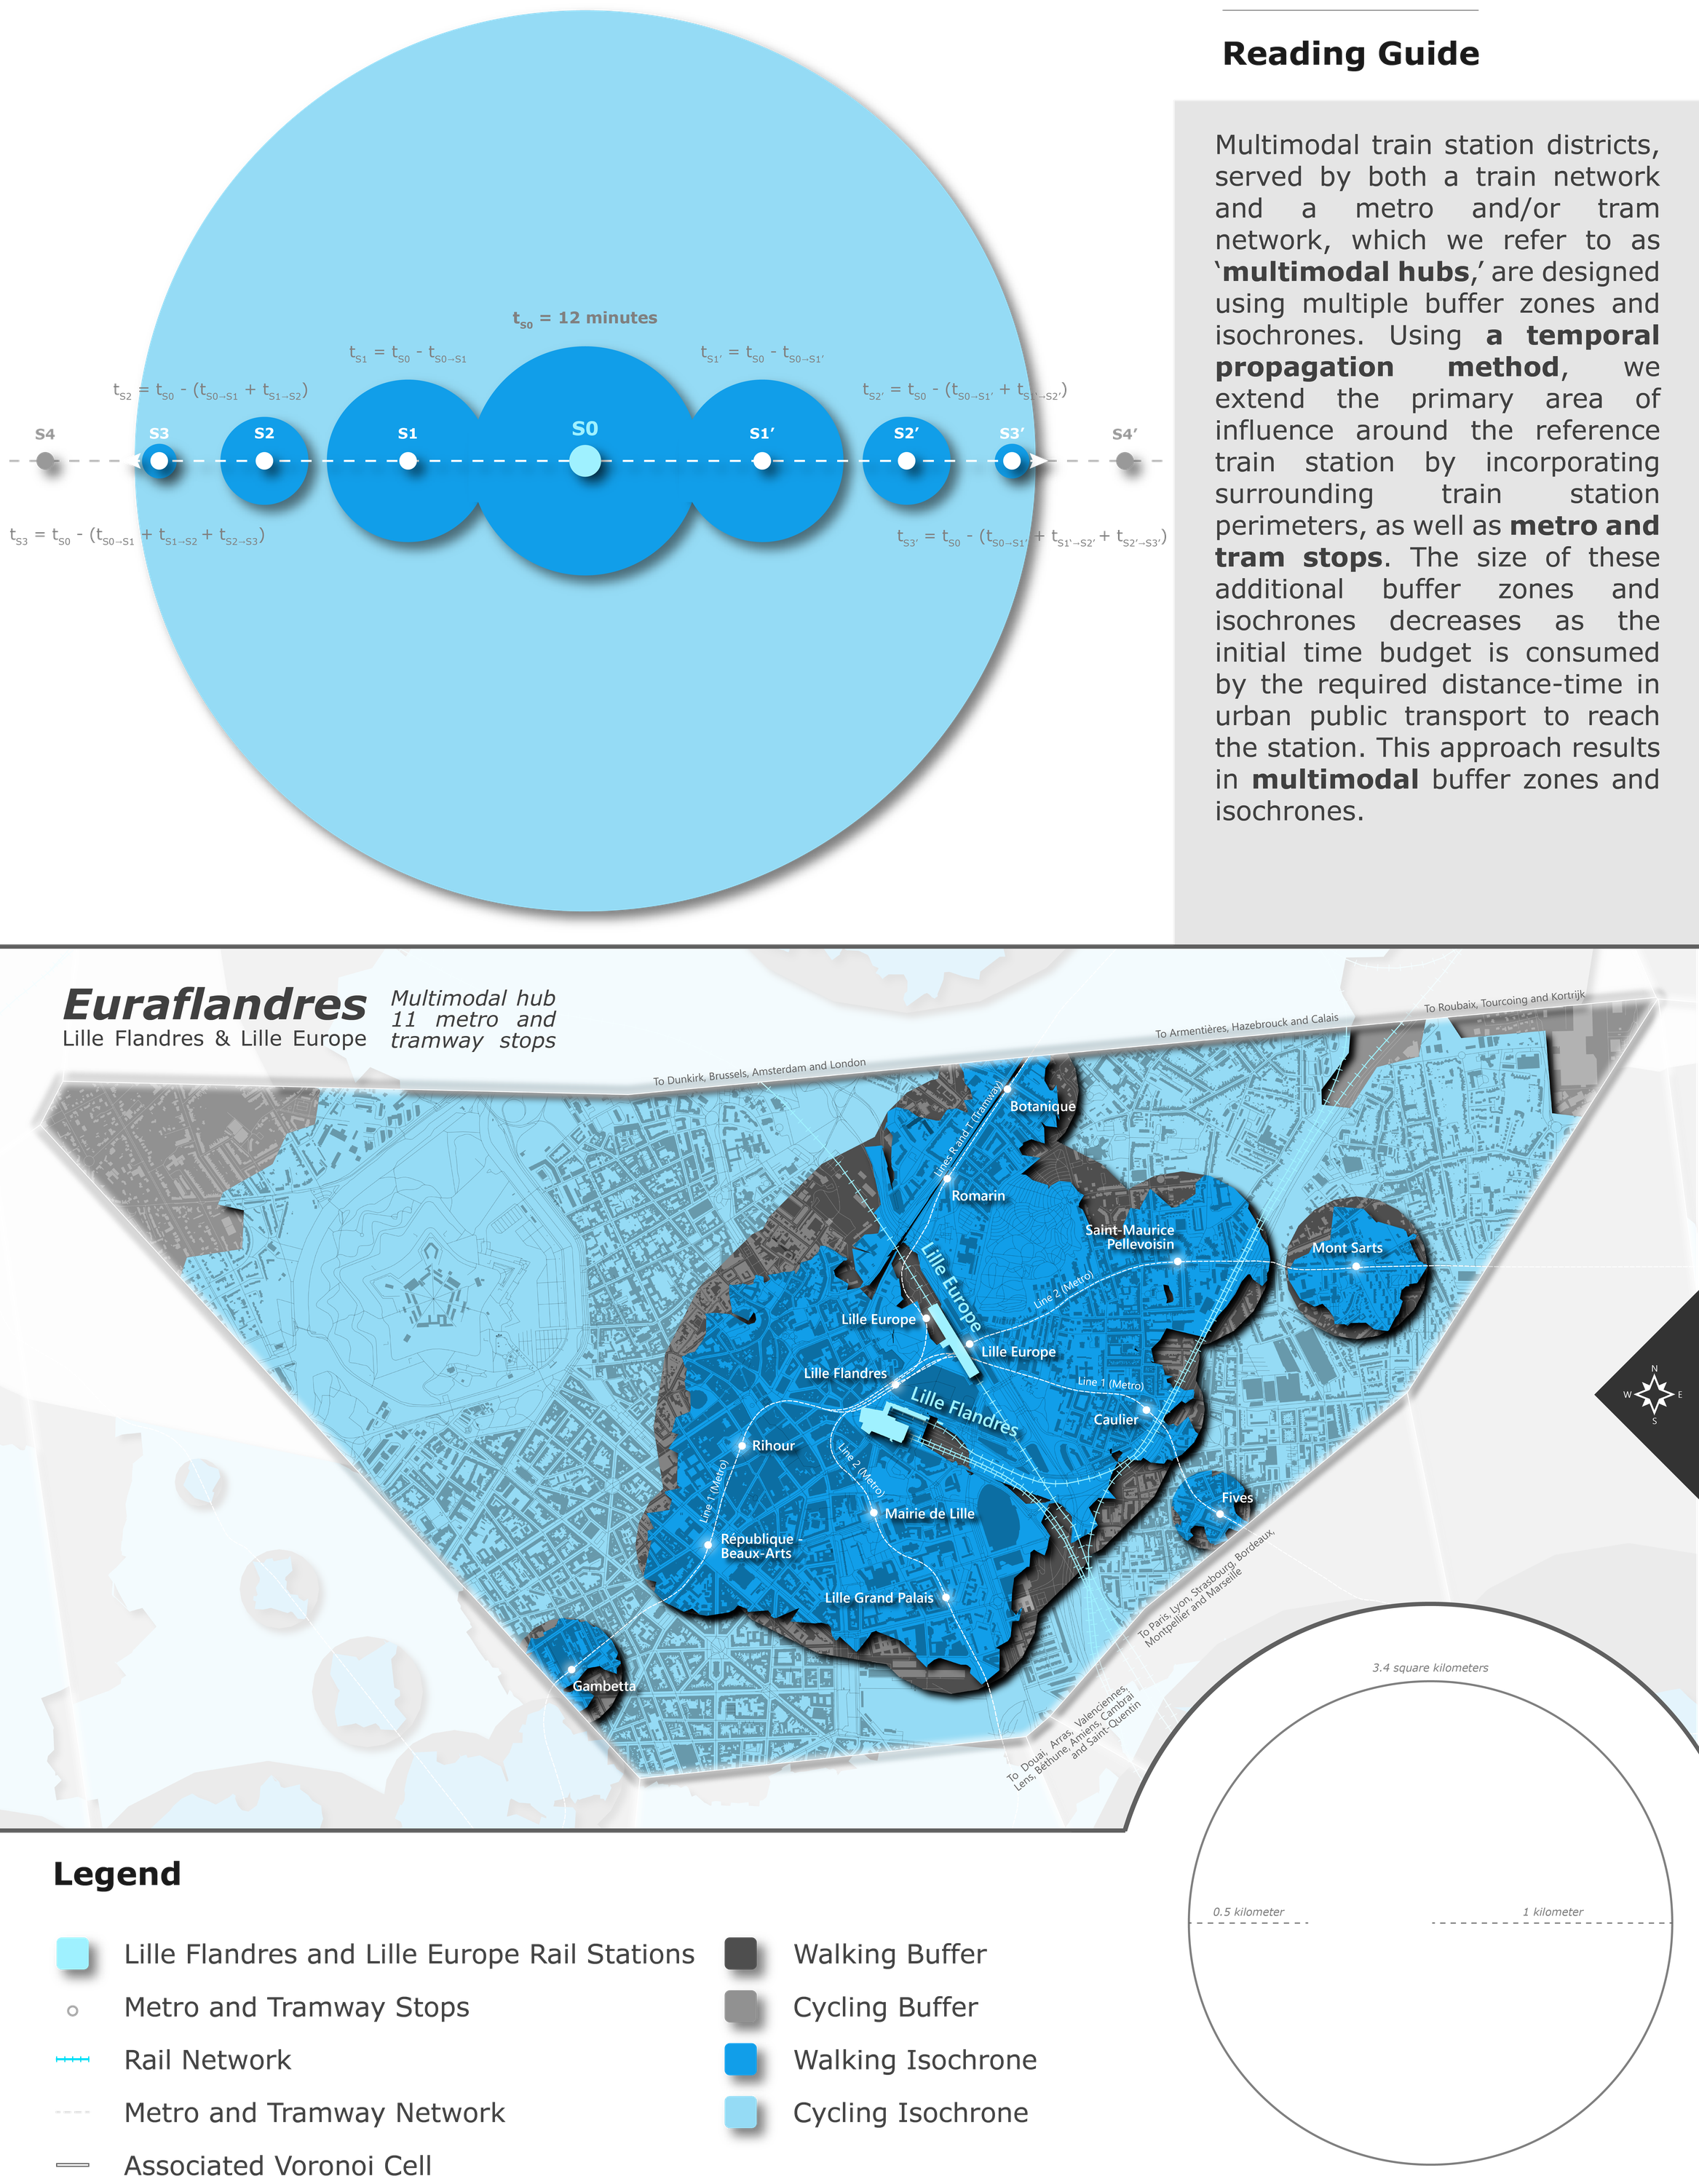
\includegraphics[width=1\columnwidth]{src/Figures/Chap-3/EN_Carte_Euraflandres.png}}
        \vspace{5pt}
        \begin{flushright}\scriptsize{
        Sources: \textcolor{blue}{\textcite{openstreetmap_openstreetmap_2023}} and \acrshort{GTFS} from \textcolor{blue}{\textcite{sncf_reseau_2024}}\index{SNCF@\textsl{SNCF}|pagebf}
        \\
        Author: \textcolor{blue}{Dylan Moinse (2024)}
        }\end{flushright}
    \end{carte}

% OTP
To implement this approach, we used the multimodal isochrone generation tool from the open-source project \Marque{OpenTripPlanner} (OTP). This tool allows for calculating accessible areas from a given point, taking into account different modes of transport as well as the possible combinations between these modes \textcolor{blue}{\autocite[15]{krismer_enhancing_2017}}\index{Krismer, Nikolaus|pagebf}, all parameters of which can be adjusted. By using the \Commas{\textsl{OTP Analyst}} module, we were able to generate isochrones representing train station neighborhoods based on their multimodal connections. In total, 5 stations in the region had their areas of influence extended to the entire multimodal approach due to their immediate proximity to metro or tram stations: \textsl{Euraflandres}\footnote{~
    We define the \textsl{Euraflandres} hub as a fusion between the Lille Flandres and Lille Europe stations (see the \hyperref[chap3:observation-quantitative-gares-examinees]{section on the stations examined}, page~\pageref{chap3:observation-quantitative-gares-examinees}).
}, Lille CHR, Roubaix, Tourcoing, and Valenciennes. These multimodal exchange hubs were designated as \Commas{multimodal hubs}. In parallel, 13 other stations belong to a second category, associated with \acrshort{HST} service, while a third category includes a total of 300 stations exclusively served by \acrshort{TER}.%%Translated%%

% Transition
Given the large number of nodes we are studying within the regional railway network, a legitimate concern arises regarding our approach to extending train station neighborhoods on foot, by bicycle, and through micromobility: the risk of territorial redundancy in spatial analyses, resulting from an excessive overlap of train station neighborhoods, particularly in certain municipalities characterized by a high density of stations. In response to this observation, we propose to combine the definition of train station neighborhoods—by adjusting their size according to the mode of transfer and the type of railway service—with a partitioning into polygonal patterns that serves to delimit each train station neighborhood.%%Translated%%

% 3.2.1.3.
\needspace{1\baselineskip} % Space reservation
\subsubsection*{Delimitation by Juxtaposition of Train Station Neighborhoods
    \label{chap3:quartiers-gare-voronoi}
    }

    % Superposition
A final concern regarding the issue of the size of train station neighborhoods lies in the question of the overlap of the influence areas as represented. In the case of a railway system, the inter-station distance is generally significant, but the extension of train station neighborhoods by incorporating light individual mobility raises the legitimate concern of an overabundance of overlapping areas. This issue is not so much a matter of aesthetics or cartographic readability, but also involves the risk of excessive analytical repetition of the same territorial configurations. For example, the \Commas{secondary} influence area of the La Madeleine station, without boundaries, encompasses the Lille Flandres and Lille Europe stations, which greatly distorts the scores for the peripheral station.%%Translated%%

% Voronoi Diagram
Since we assume that users of light individual mobility, entering or leaving a station, aim to take the shortest path \textcolor{blue}{\autocite[116]{heran_distances_2009}}\index{Héran, Frédéric|pagebf}, we opted for a partition of the regional railway network to define the theoretically closest areas, from a geometric perspective, to each station. This division, based on an Euclidean plane, allows us to model and visualize the theoretical maximum coverage of each influence area, represented by a cell from a standard Voronoi diagram \textcolor{blue}{\autocite[479]{mota_method_2014}}\index{Mota, Diego Rosa|pagebf}\index{Takano, Marise|pagebf}\index{Taco, Pastor Willy Gonzales|pagebf}. This approach, which aims to avoid any form of overlap, considers that each cell corresponds to a space where all points are closer to the associated station than to any other station, regardless of the hierarchy of the railway network \textcolor{blue}{\autocite[429]{lebedeva_increasing_2018}}\index{Lebedeva, Olga|pagebf}\index{Kripak, Marina|pagebf}\index{Gozbenko, Valeriy|pagebf}.%%Translated%%

% Transition
To represent the geographical perimeter of the 318 stations that make up the Hauts-de-France railway network, our analysis first focused on determining the size of the different catchment areas. This approach initially involved distinguishing between the train station neighborhoods limited to the acceptable walking distance combined with walking, and those extended by the use of bicycles and micromobility. Subsequently, a differentiation was made between stations connected to the \acrshort{TER} network, those linked to the \acrshort{HST} network, and multimodal exchange hubs. Finally, a confinement of the maximum reach of each public transport node was established, delimiting it within boundaries. The spatialization of the four types of train station neighborhoods within the regional network can be visualized on \hyperref[fig-chap5:aires-influence]{Map~\ref{fig-chap5:aires-influence}} (page~\pageref{fig-chap5:aires-influence}) of the \hyperref[chap5:titre]{Chapter~5} (page~\pageref{chap5:titre}). Once the sizes were defined and integrated into the methodological protocol, our focus now shifts to the morphology of these train station neighborhoods, particularly the shapes they can take and the ways in which they can be represented.%%Translated%%

% 3.2.2.
\needspace{1\baselineskip} % Space reservation
\subsection{Morphology and Contours of Train Station Neighborhoods
    \label{chap3:quartiers-gare-formes}
    }

    % Introduction
The question of the shape of train station neighborhoods seems, to our knowledge, much less explored in the scientific and technical literature. This can be explained by the complexity it entails, both at the level of territorial structures and technical considerations, requiring advanced mastery of the tools needed to generate various types of influence areas. While the topic of buffer zones, their limitations, and the value of adopting isochrones, or even combining them to create an interesting synergy, is relatively well documented, the discussion around their rendering and representation remains critical. It is in this sub-section that we define two forms of train station neighborhoods—the buffer zones (\(B\)) and the isochrone curves (\(I\))—which complement the reflection on the size of their perimeters (\(P\) and \(B\)). However, their visualization remains a central issue. For this reason, we have chosen to delve deeper into the various ways of representing these neighborhoods, with the aim of developing a methodological approach to design our own buffer zones and isochrones. This cartographic line of thought relies on a combination of computational and visual techniques.%%Translated%%

% 3.2.2.1.
\needspace{1\baselineskip} % Space reservation
\subsubsection*{Integration of Urban Cutoff Effects
    \label{chap3:quartiers-gare-isochrones-buffers}
    }

    % Buffers
Even today, the majority of studies, whether academic or operational, rely on the use of theoretical buffers to represent the catchment areas of public transport stations. These buffer zones are represented by circles drawn at a fixed distance, whether spatial or temporal, around transport nodes, without considering surrounding networks or geographical obstacles. This method has the advantage of being simple to produce and easy to interpret, as it requires neither complex data nor advanced calculations. It also offers great versatility, being applicable to various types of infrastructure, even beyond issues strictly related to mobility. However, this technique for producing train station neighborhoods faces major limitations. By relying on a representation of straight-line distances on an Euclidean plane, it ignores transport networks as well as the geographical constraints of the physical environment. Consequently, buffer zones do not reflect the actual accessibility of infrastructures. Such simplification can lead to inaccurate conclusions, particularly in contexts where the configuration of networks and territories plays a decisive role in defining train station neighborhoods.%%Translated%%

% Urban Cutoff Effects
The issue of correcting straight-line distances to obtain real distances is not merely technical. It requires reflection on the effects of urban cutoff, as well as an inquiry into the origins of detours, which involves analyzing the configuration of the road network, its grid, and its hierarchy \textcolor{blue}{\autocite[119]{heran_distances_2009}}\index{Héran, Frédéric|pagebf}. An urban cutoff is defined as an obstruction that disrupts the relationships between surrounding populations. This obstruction can be of natural or artificial origin, built or unbuilt. The effect of urban cutoff manifests as linear or surface obstructions, causing physical or psychological disruptions \textcolor{blue}{\autocite[4]{heran_zones_2009}}\index{Héran, Frédéric|pagebf}\index{Pouillaude, Laurence|pagebf}. Among the most emblematic effects of urban cutoff are highways or urban forms, as well as rivers or mountains. Paradoxically, railway infrastructures themselves can contribute to these cutoff effects. The Franco-German research-action report \textsl{Bahn.Ville 2} illustrates this issue by showing how railway tracks contribute to the creation of urban cutoffs, thus reinforcing a negative \gls{perception}, or even the invisibility, of rail in the urban space \textcolor{blue}{\autocite[20]{lhostis_concevoir_2009}}\index{L'Hostis, Alain|pagebf}\index{Alexandre, Elsa|pagebf}\index{Appert, Manuel|pagebf}\index{Araud-Ruyant, Catherine|pagebf}\index{Basty, Marius|pagebf}\index{Biau, Géraldine|pagebf}\index{Bozzani-Franc, Sandra|pagebf}\index{Boutantin, Gratienne|pagebf}\index{Constantin, Chantal|pagebf}\index{Coralli, Monica|pagebf}\index{Durousset, Marie-Jeanne|pagebf}\index{Fradier, Christophe|pagebf}\index{Gabion, Cyrille|pagebf}\index{Leysens, Thomas|pagebf}\index{Mermoud, Françoise|pagebf}\index{Olny, Xavier|pagebf}\index{Perrin, Emmanuel|pagebf}\index{Robert, Jean|pagebf}\index{Simand, Noémie|pagebf}\index{Stransky, Vaclav|pagebf}\index{Soulas, Claude|pagebf}\index{Verdier, Anne-Marie|pagebf}\index{Vulturescu, Bogdan|pagebf}. Therefore, urban cutoff is an important element for understanding the interactions between the railway system and territories.%%Translated%%

% Isochrones
It is in this context that isochrones are frequently considered a more realistic representation of accessible areas. Unlike buffer zones, they delineate the spaces that can be reached within a given time, from or to a station, while integrating infrastructures and modes of transport. By considering the road network as well as the specificities of different modes of transport—primarily their range, speed, and the areas they are able to cross—isochrones offer a more accurate representation of accessibility. Due to their ability to reflect real spatial dynamics, isochrone modeling serves as a precise tool for evaluating the areas that are actually accessible. The first occurrences in the field of geography date back to the early 20\textsuperscript{th} century, such as the \textsl{isochrone lines} drawn by \textcolor{blue}{Joseph} \textcolor{blue}{\textcite[311-314]{letaconnoux_note_1907}}\index{Letaconnoux, Joseph|pagebf}, depicting the evolution of accessibility in Brittany since the 18\textsuperscript{th} century. In urban planning, typically pedestrian, isochrones first found use in the work of \textcolor{blue}{Jane} \textcolor{blue}{\textcite[179-182]{jacobs_death_1961}}\index{Jacobs, Jane|pagebf}, who introduced the concept of \textsl{pools of use} to refer to areas within walking distance of a specific urban location, based on the travel time \textcolor{blue}{\autocite[3]{dovey_isochrone_2017}}\index{Dovey, Kim|pagebf}\index{Woodcock, Ian|pagebf}\index{Pike, Lucinda|pagebf}. For example, the \acrfull{MEL}, formerly \acrfull{LMCU}, mapped in 2000 the \acrfull{ZAP} and \acrfull{ZAV} around its heavy public transport stations. These isochrone curves were designed to identify strategic metropolitan development locations \textcolor{blue}{\autocite[9]{heran_zones_2009}}\index{Héran, Frédéric|pagebf}\index{Pouillaude, Laurence|pagebf}.%%Translated%%

% Isodistances
In a similar approach aimed at surpassing the idea of straight-line distances defined by buffer zones, we find isodistance curves, often confused with isochrones. However, a fundamental distinction exists: isodistances refer to areas that group all points located at a real spatial distance, measured on a network, from a reference point such as a public transport station. Derived from the Greek \textsl{isos} (equal) and \textsl{khronos} (time), the term isochrone differs from isodistance, which refers to an area defined by a real spatial distance, distorted by the network, but independent of speeds or travel times. Isodistance thus illustrates an isometric catchment area, in contrast to the isochrone, which is based on a temporal distance. This frequent confusion can be explained by the predominance of pedestrian accessibility studies around stations. These studies often assume that the relatively homogeneous speeds of pedestrians lead to an overlap of isochrone curves and isodistance curves \textcolor{blue}{\autocite[9]{heran_zones_2009}}\index{Héran, Frédéric|pagebf}. However, in the case of cycling mobility, these similarities tend to fade. The much more variable speeds of light individual mobility, influenced by road hierarchy, the quality of infrastructure, or individual factors such as the type of vehicle or the cyclists' skills, highlight the need to clearly differentiate these concepts.%%Translated%%  

% Combination of Isochrones and Buffers
During the course of our doctoral work, we favored the combined use of buffer zones, isodistances, and isochrones. Their combination in spatial analysis provides an integrated perspective on accessibility. By overlaying isodistances or isochrones with buffer zones, it becomes possible to measure accessibility differentials, that is, the gap between actual accessibility and theoretical accessibility. This confrontation also allows for the calculation of the service coverage rate, which expresses the ratio between the area that is actually accessible and the area reachable in a straight line \textcolor{blue}{\autocite[13]{heran_zones_2009}}\index{Héran, Frédéric|pagebf}. The cartographic diagnosis of these different representations of train station neighborhoods allows for a systematic identification of the obstacles faced by travelers.%%Translated%%

% Transition
Once the debate on the benefits of isochrones is overcome—a necessary step, but one that seems, according to our observations, increasingly accepted and commonly integrated into various studies—the question of their representation arises. While the advantages of isochrones, especially for integrating the physical obstacles present in the territories, are widely recognized in research practices, it appears that their rendering varies significantly and often lacks transparency regarding the parameters used. This opacity can be explained by the fact that most of them are generated using platforms that limit control over the modeling parameters. In light of this, we set out to develop our own train station neighborhoods using a custom script, thus giving us the ability to define geographic boundaries tailored to our research objectives.%%Translated%%

% 3.2.2.2.
\needspace{1\baselineskip} % Réserve de l'espace
\subsubsection*{Reflection on the Cartographic Representation of Train Station Neighborhoods
    \label{chap3:quartiers-gare-python}
    }

% Creating Influence Areas: Python (Geographic Precision)
A thorough reflection is required to establish cartographic representation strategies for accessibility zones, such as buffer zones and isochrones, in line with the objectives of this doctoral research. This approach is not only about aesthetic or communication considerations, but also aims to ensure control, both in substance and form, over the geographic analysis foundations used throughout this work. First and foremost, it is important to clarify the concepts involved, particularly by identifying the parameters that influence the configuration of representations and the analytical interpretations that follow. Given the variety of tools available for generating buffer zones and isochrones, we chose to continue our analysis using the Python programming language. This choice is based not only on the richness of the libraries offered by this environment but also on the transparency provided by the open-source tool, which allows full control over the defined parameters\footnote{~
    Python is a general-purpose language applicable to many fields and has become increasingly popular among data scientists \textcolor{blue}{\autocite[19]{velt_python_2020}}\index{Velt, Amandine|pagebf}. In addition to its extensive documentation, Python features a graphical interface for data analysis and sharing analyses: Jupyter Notebooks. A notebook is an executable document whose results are integrated into the document, along with text or mathematical equations. Thus, the Jupyter Notebook tool and the use of Python, accompanied by useful libraries such as Pandas and GeoPandas, were widely used in our analyses to ensure greater transparency and better teamwork management \textcolor{blue}{\autocite[55, 137]{velt_python_2020}}\index{Velt, Amandine|pagebf}.
}.%%Translated%%

% Isochrone to and from
The first parameter that questions the geographic construction of train station influence areas lies in the direction of the flows. At first glance, it might seem intuitive to assume that, regardless of the flow direction—whether it is a feeder trip to the station or a distribution from it—the train station neighborhood would retain a similar size and shape. However, this assumption tends to overlook two dimensions: road connectivity, which is particularly crucial for bicycles and micromobility, governed by traffic regulations, as well as temporality. Indeed, an isochrone directed toward or from a station does not necessarily have the same validity depending on factors such as the operating hours of the lines or the directions served. Concerning our empirical data, we decided to consider that, by default, the buffer zones and timeless isochrones are designed to analyze the areas accessible toward the station, and not in the opposite direction, as is often the case. This choice is explained by the primacy of the access logic, which is prioritized because bicycles, when used in connection with stations, are much more frequently used in access than in egress.%%Translated%%

% Surface VS roads VS built environment VS POIs
The issue of cartographic representation of isochrones, whether in their analytical dimension or communicative function, also arises in terms of the choice of structural elements to highlight. Should we prioritize a visual representation of accessible or inaccessible surface area? Or would it be more relevant to highlight the road network, which materializes the connections used for isochrone calculation? Another possibility would be to emphasize the built environment or the \acrfull{POIs}, which ultimately represent the destinations individuals are trying to reach. These cartographic choices are not neutral, as they guide the reading and interpretation of the data while influencing how the results are communicated to the various target audiences.%%Translated%%

% Isochrone road network
The representation based on the road network directly reflects the achievable paths within a defined pedestrian or cycling network. This visualization method aims to offer a more realistic approach by taking into account the physical constraints of movement, while being particularly suited for navigation and cartographic landmarks\footnote{~
    The most well-known \acrfull{API} for creating road-based isochrones is certainly the one developed by \textcolor{blue}{\textcite{graphhopper_visualization_2018}}.
}. However, such a representation can also lead to some visual complexity, making interpretation more difficult for some users. Beyond simple polygons, it provides a detailed representation of accessible road segments, directly viewable in a browser. For illustrative purposes, we applied this method, using our own code, to represent, in both a plane projection and a volumetric model, the isochrone accessible via individual mobility to the Amiens train station. This representation relies on the road network directly accessible to cyclists (see \hyperref[fig-chap3:isochrone-amiens-voirie]{Map~\ref{fig-chap3:isochrone-amiens-voirie}}, page~\pageref{fig-chap3:isochrone-amiens-voirie})\footnote{~
    This cartographic analysis was enhanced by the use of color transparency, which highlights the flow matrices. The effectiveness of this technique combined with a dark background lies in optimizing \Commas{visual salience}~–~this concept refers to the alignment between the represented phenomenon, the visual variables used, and their perception by the observer~–~of the represented elements and the information conveyed, while facilitating the perception of complex geometries. This approach ensures better readability, as demonstrated by \textcolor{blue}{Françoise} \textcolor{blue}{\textcite[226]{bahoken_contribution_2016}}\index{Bahoken, Françoise|pagebf}, in her doctoral thesis, based on a cartography of a flow matrix.
}.%%Translated%%

% Isochrone Amiens road network map
\begin{carte}[h!]\vspace*{4pt}
    \caption{Cartographic representation of the accessible road network by bike and micromobility to the Amiens train station, constructed from an isochrone.}
    \label{fig-chap3:isochrone-amiens-voirie}
    \centerline{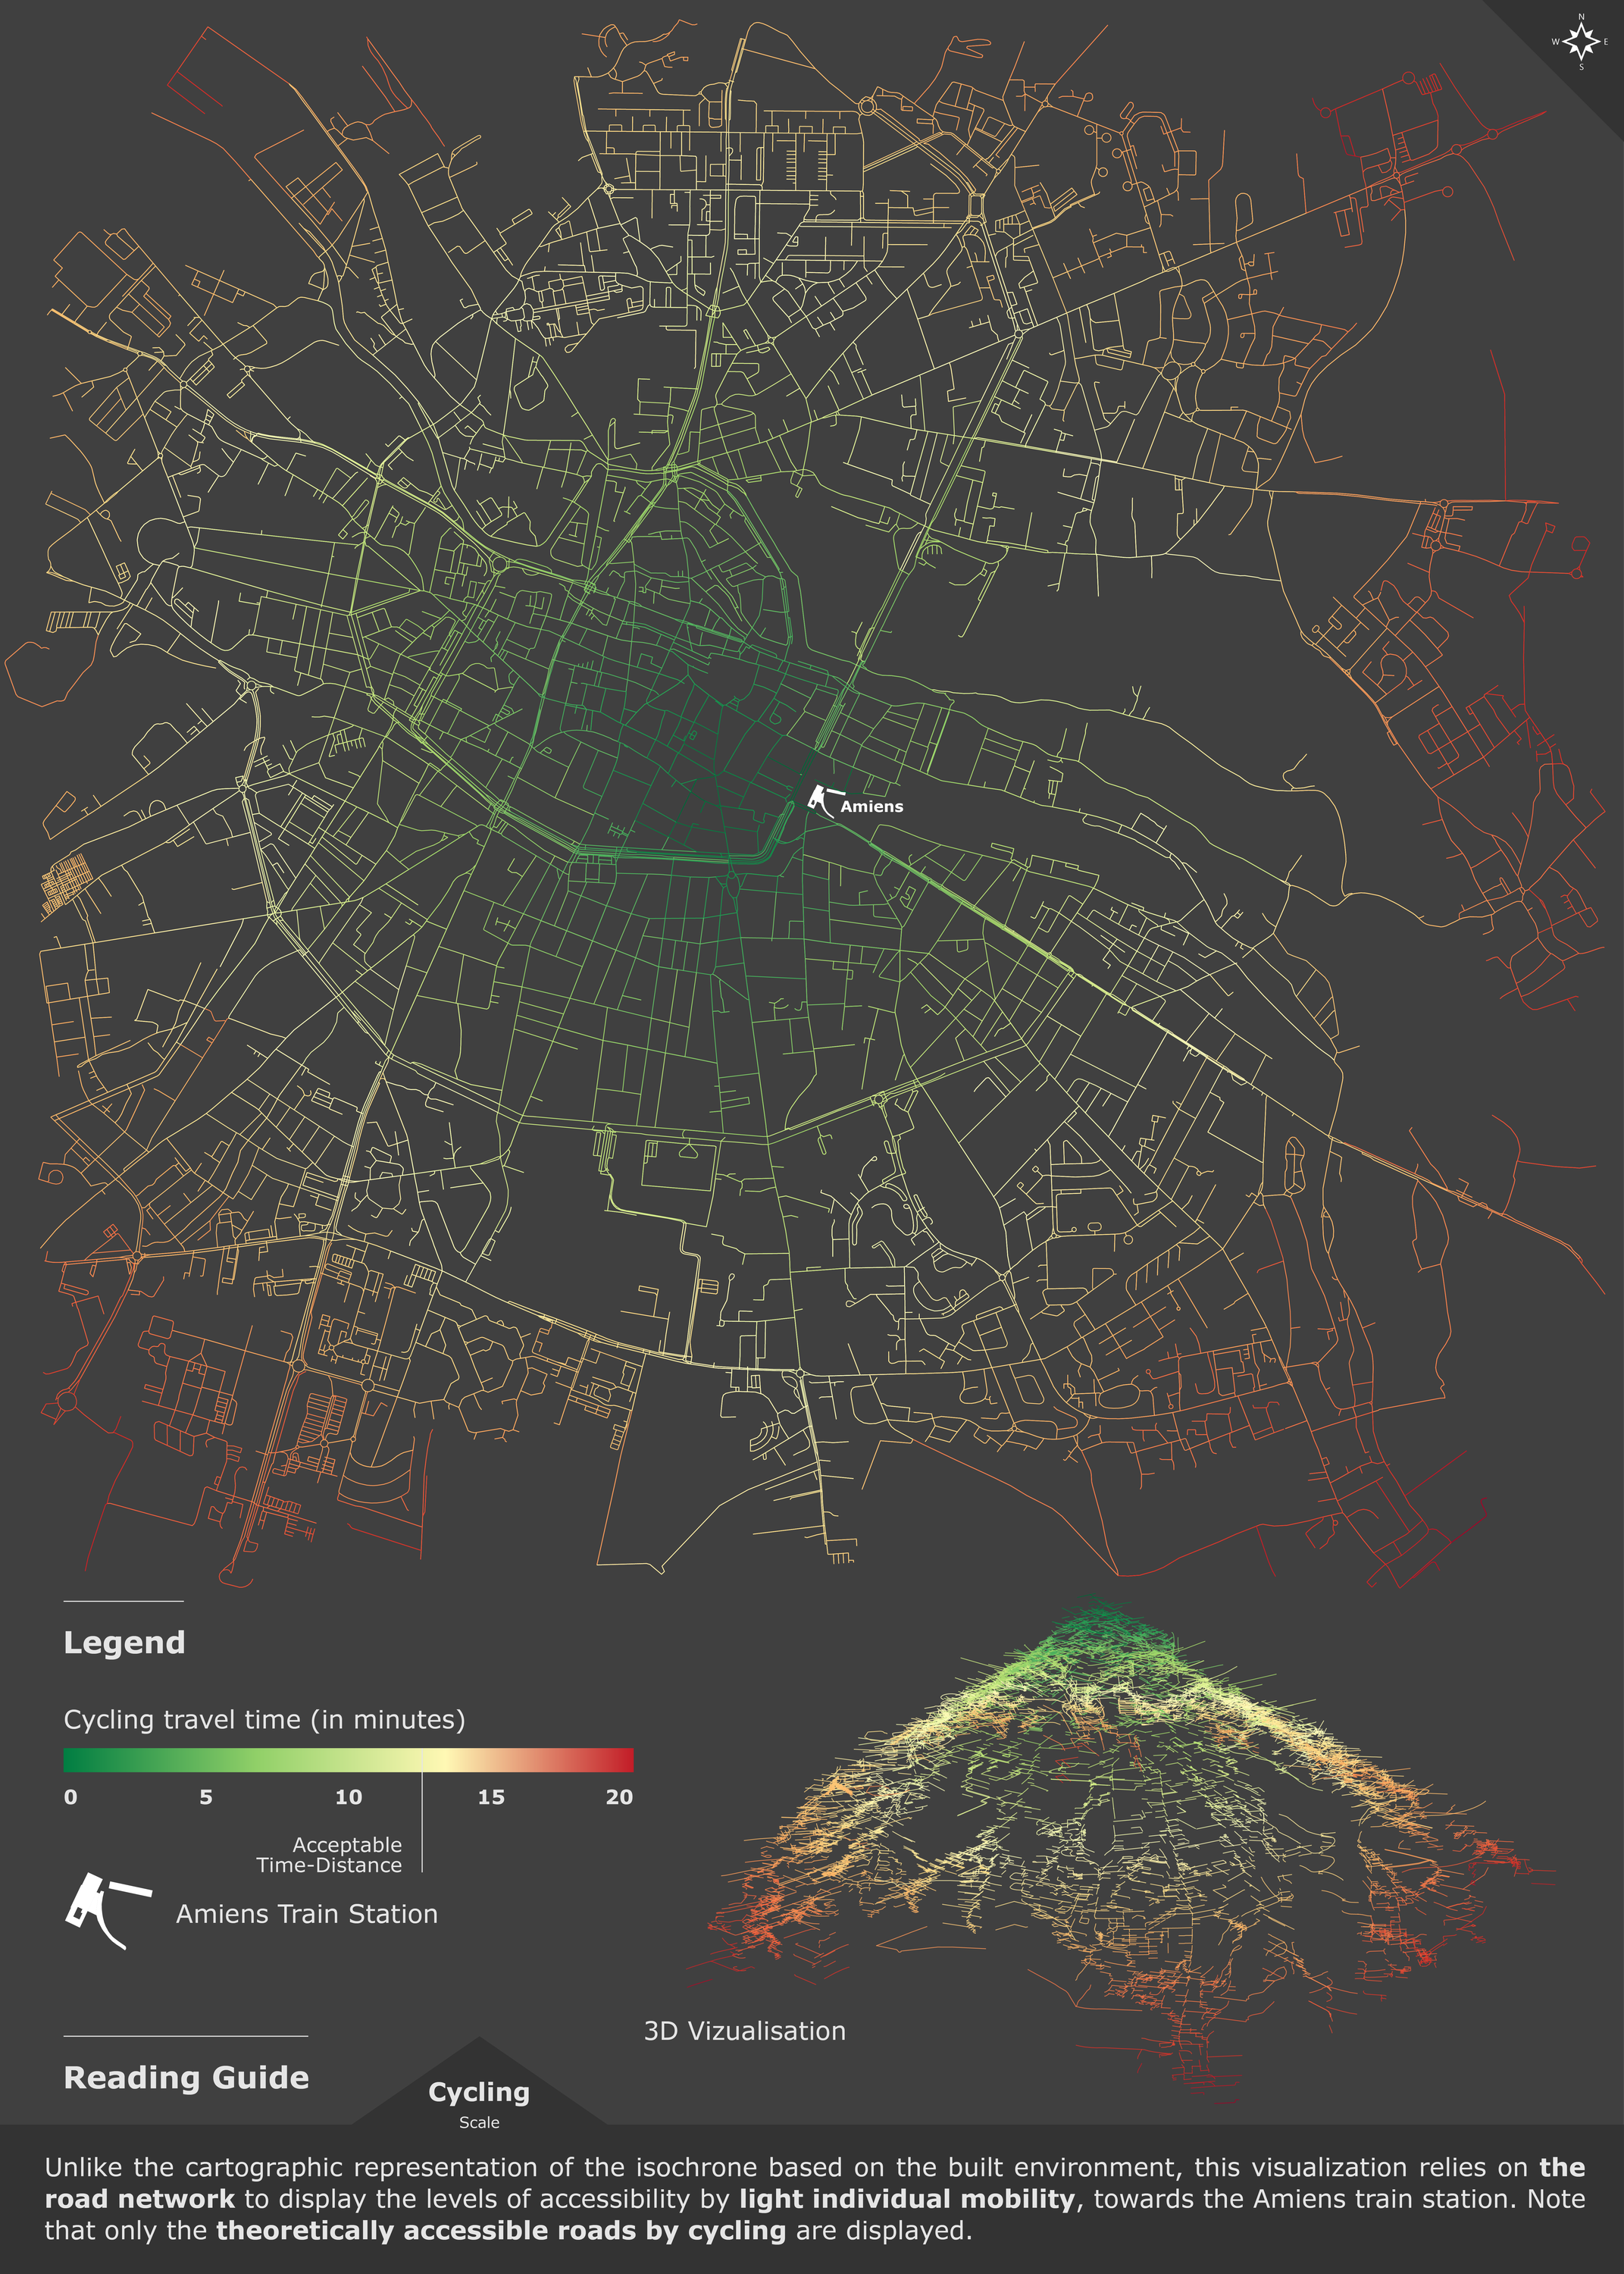
\includegraphics[width=1\columnwidth]{src/Figures/Chap-3/EN_Carte_Isochrone_Amiens_Voirie.png}}
    \vspace{5pt}
    \begin{flushright}\scriptsize{
    Sources: \textcolor{blue}{\textcite{openstreetmap_openstreetmap_2023}} and \acrshort{GTFS} from \textcolor{blue}{\textcite{sncf_reseau_2024}}\index{SNCF@\textsl{SNCF}|pagebf}
    \\
    Author: \textcolor{blue}{Dylan Moinse (2024)}
    }\end{flushright}
\end{carte}

% Isochrone built environment
Regarding the representation based on the built environment or the accessible \acrshort{POIs} within the allotted time, it has the advantage of better addressing user needs by focusing attention on the places where individuals directly interact, such as residences, workplaces, stores, and public facilities (see \hyperref[fig-chap3:isochrone-amiens-bati]{Map~\ref{fig-chap3:isochrone-amiens-bati}}, page~\pageref{fig-chap3:isochrone-amiens-bati}). This approach is particularly relevant for analyses focused on specific services, providing an immediate and practical response to the question of service accessibility. However, this form of visual representation has certain limitations. It excludes undeveloped areas, which still represent a need in terms of accessibility, such as green spaces or other open areas with functional or social value. Moreover, it does not highlight the overall connectivity of the area.%%Translated%%

% Isochrone built environment map
\begin{carte}[h!]\vspace*{4pt}
    \caption{Cartographic representation of the built environment accessible by bike and micromobility towards the Amiens train station, created using an isochrone.}
    \label{fig-chap3:isochrone-amiens-bati}
    \centerline{\includegraphics[width=1\columnwidth]{src/Figures/Chap-3/EN_Carte_Isochrone_Amiens_Bati.png}}
    \vspace{5pt}
    \begin{flushright}\scriptsize{
    Sources: \textcolor{blue}{\textcite{openstreetmap_openstreetmap_2023}} and \acrshort{GTFS} from \textcolor{blue}{\textcite{sncf_reseau_2024}}\index{SNCF@\textsl{SNCF}|pagebf}
    \\
    Author: \textcolor{blue}{Dylan Moinse (2024)}
    }\end{flushright}
\end{carte}

% Advantages and disadvantages of isochrone types
In a comparative manner, we can establish that isochrones, traditionally represented as accessible areas, offer the advantage of great visual clarity, generally require a limited volume of geographical data, and are suited for global analyses. Unlike the representation based on road networks, which is more precise but more suited to specific uses such as navigation, which are less relevant in the context of our research issue. Finally, representations based on the built environment or on accessible facilities and services within an area have the merit of offering a more user-centric perspective. They are well-suited for urban analyses, particularly concerning urban forms and accessibility to targeted services. However, this type of cartographic representation is more demanding in terms of data and incurs higher mapping costs.%%Translated%%

% Final Isochrone: Playing on the edges
In this perspective, we chose to combine the forms of cartographic representation we have experimented with, relying on the production of hybrid isochrones: surface-based, certainly, but whose shape primarily depends on the road network while being influenced by the presence of surrounding built environment (see \hyperref[fig-chap3:isochrone-amiens-finale]{Map~\ref{fig-chap3:isochrone-amiens-finale}}, page~\pageref{fig-chap3:isochrone-amiens-finale}). Adopting this technique allowed us to produce cartographic representations with contours much more precise than the approximations often observed in traditional isochrone productions. In this approach, we relied on the innovative method developed by software developer and researcher \textcolor{blue}{Kuan} \textcolor{blue}{\textcite{butts_better_2017}}\index{Butts, Kuan|pagebf}, based on the \textsl{OSMnx} tool, available in the \textsl{Python} programming language, and specifically designed to model road networks \textcolor{blue}{\autocite[132]{boeing_osmnx_2017}}\index{Boeing, Geoff|pagebf}. This approach aligns with the concept of an isochrone map built based on the road network (\textsl{lines}), adopting a graph theory logic (\textsl{edges}), while incorporating a linear buffer around each accessible road and intersection (\textsl{buffers}). This process therefore allows the incorporation of urban elements adjacent to the road network \textcolor{blue}{\autocite[135]{boeing_osmnx_2017}}\index{Boeing, Geoff|pagebf}, without using them in the representation, as seen in \hyperref[fig-chap3:isochrone-amiens-bati]{Map~\ref{fig-chap3:isochrone-amiens-bati}} (page~\pageref{fig-chap3:isochrone-amiens-bati}).%%Translated%%

% Final Isochrone Map adopted for Amiens
\begin{carte}[h!]\vspace*{4pt}
    \caption{Cartographic representation of the isochrone accessible by bicycle and micromobility to the Amiens station, overlaid with the road network.}
    \label{fig-chap3:isochrone-amiens-finale}
    \centerline{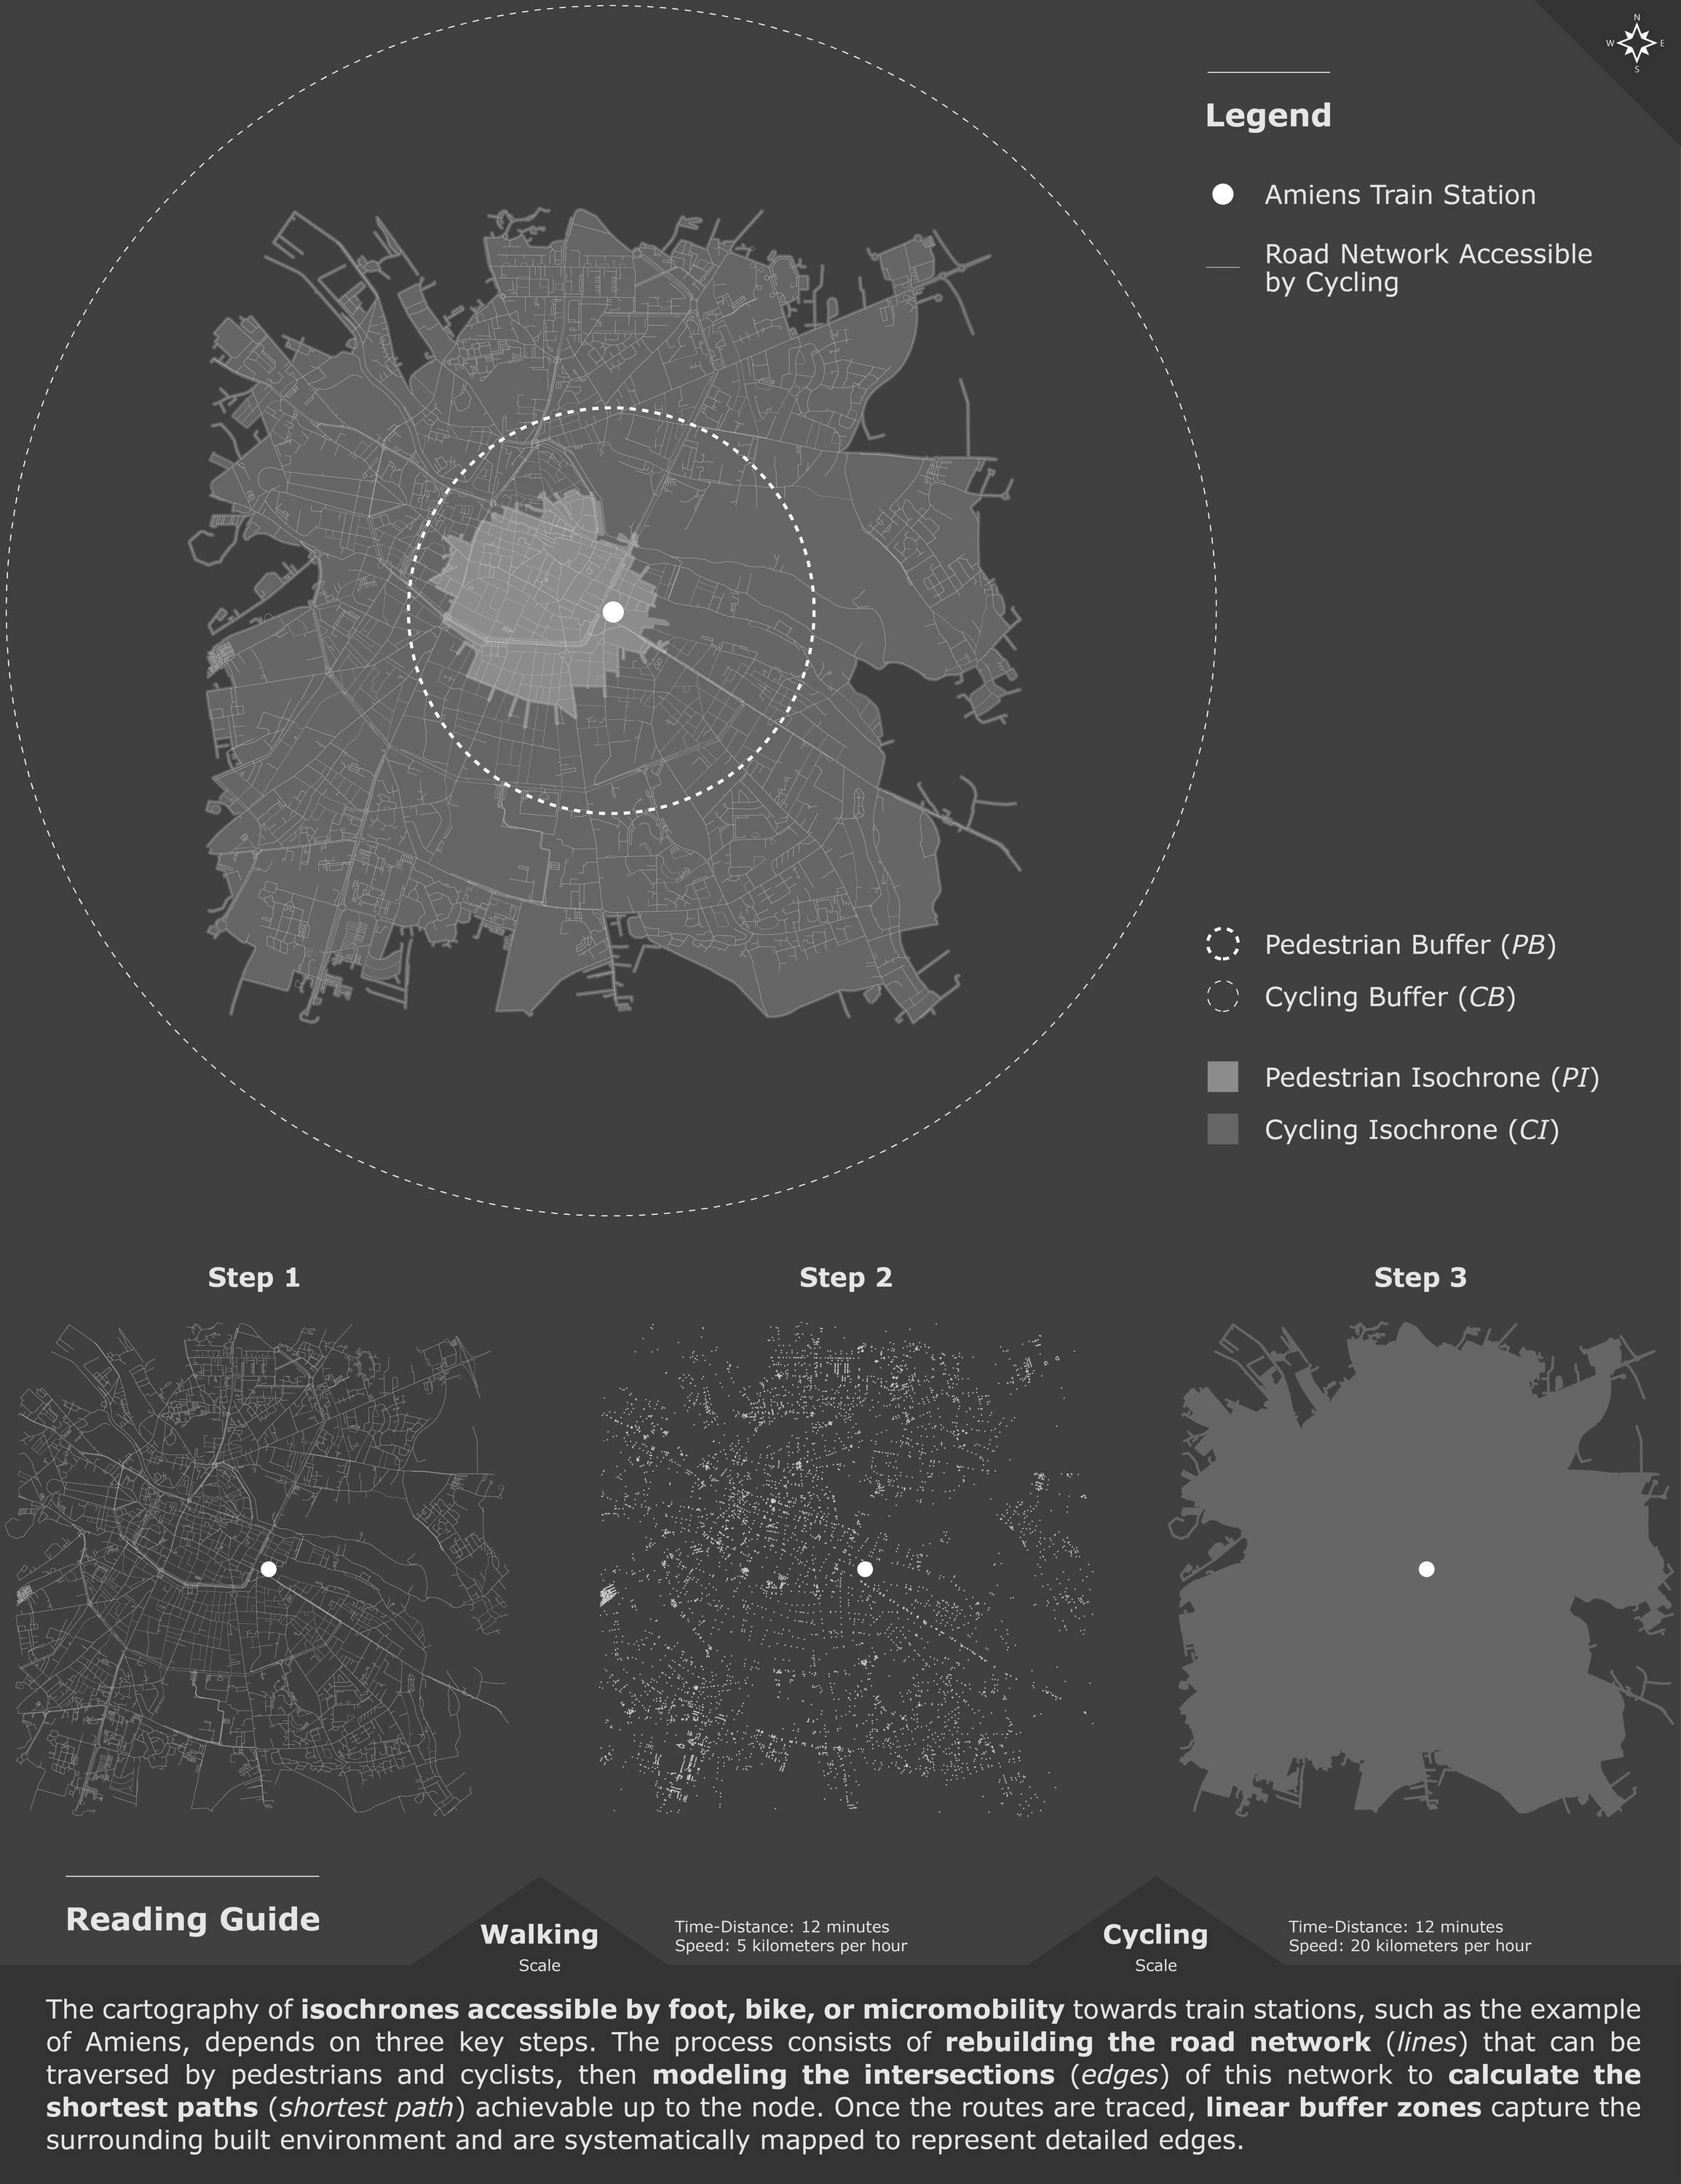
\includegraphics[width=1\columnwidth]{src/Figures/Chap-3/EN_Carte_Isochrones_Buffers_Amiens.png}}
    \vspace{5pt}
    \begin{flushright}\scriptsize{
    Sources: \textcolor{blue}{\textcite{openstreetmap_openstreetmap_2023}} and \acrshort{GTFS} from \textcolor{blue}{\textcite{sncf_reseau_2024}}\index{SNCF@\textsl{SNCF}|pagebf}
    \\
    Author: \textcolor{blue}{Dylan Moinse (2024)}
    }\end{flushright}
\end{carte}

% Accessible/Non-accessible Zones and Transition
Many questions have guided, and could still guide, this subsection, which primarily focuses on a global reflection on the morphology of the generated isochrones. For example, we could have also discussed the visual hierarchy between the \textsl{visible} and the \textsl{invisible}. If the goal is to highlight accessible areas, wouldn't it be more pertinent to color or mask the non-accessible areas? This would not only refocus attention on the accessible spaces but also visually free up the cartographic space to integrate symbols and additional elements, without them being visually disturbed by the isochrone. As \textcolor{blue}{Jacques} \textcolor{blue}{\textcite[5]{levy_tournant_1999}}\index{Lévy, Jacques|pagebf} points out in his seminal work \textsl{Le tournant géographique. Penser l'espace pour lire le monde}, the process of delimitation and differentiation contributes to the formation of geographic spaces. This principle, which we have briefly explored here, now leads us to explain the geographic data collection and analysis techniques employed once the station districts—as the preferred geographic areas of our study area—are defined.%%Translated%%

% 3.2.3.
\needspace{1\baselineskip} % Reserve space
\subsection{Geostatistical Analysis of Mapped Station Districts
    \label{chap3:quartiers-gare-analyse-geostatistique}
    }

    % Introduction
The effort spent on the geographical production of station districts with varying sizes and shapes would be meaningless if the data integrated into them were aggregated at too broad scales, such as that of the municipality. Relying solely on such administrative boundaries would neither reflect the individuality of each station district nor capture the distinctions between their different types or the internal variations within each of them. By raising this issue, we established as a methodological rule to limit ourselves to disaggregated databases, in the form of point, line, or polygon vectors, independent of grids or administrative boundaries. However, due to the scarcity of available open data, despite France's advantageous position with its proactive centralization of data sets, it is sometimes necessary to rely on aggregated data, for anonymization purposes, for example. Thus, in the second phase, we propose an estimation method based on aggregated data at the scale of regular grids. This approach allows us to circumvent the limitations while maintaining sufficient analytical precision for the needs of our research.%%Translated%%

% 3.2.3.1.
\needspace{1\baselineskip} % Reserve space
\subsubsection*{Disaggregated Spatial Data
    \label{chap3:quartiers-gare-donnees-desagregees}
    }

    % Geocoded disaggregated data without administrative boundaries
The study of the delineated station districts in the region is entirely based on the use of disaggregated geographical data. This methodological approach aims to ensure analytical robustness, while providing sufficient granularity to explore the specific local dynamics of these strategic spaces. Disaggregated geographical data are characterized by their high level of detail and their independence from administrative divisions or predefined boundaries. They are available in several forms: points, representing the exact location of facilities; or detailed polygons, illustrating land footprints, for example.%%Translated%%

% Data Sources
Unlike aggregated data, which are typically collected at large scales, disaggregated data allow for the analysis of territories at a micro-local or even ultra-local scale. The value of adopting a detailed view of station districts, independent of municipal boundaries 
\textcolor{blue}{\autocite[7]{moretti_interconnexion_1999}}\index{Moretti, Anna|pagebf}\index{Vacheret, Guy|pagebf}, is of major importance. The data used in our study come from various official sources, combined to form a coherent set that can be processed in a \acrfull{GIS} tool or as computer code to generate graphical elements usable in a geographical context. In our case, \Commas{geocoding} refers to code written in \textsl{Python}. These sources include, in particular, open data, disaggregated socio-economic databases, and cadastral databases. This data integration ensures a detailed and contextualized representation of station districts, tailored to the analytical and methodological requirements of this research.%%Translated%%

% Advantages and Transition
While station districts, far from being homogeneous, exhibit micro-dynamics often imperceptible at larger scales, disaggregated analysis highlights these territorial disparities. These data also allow for the modeling of spatial and functional interactions with great precision. This granularity avoids biases induced by territorial divisions and promotes the exploration of spatial logics based on usage. The station districts, in constant evolution, also benefit from disaggregated data to ensure precise and timely tracking of these transformations. However, these disaggregated databases remain relatively scarce and are sometimes affected by limitations related to the quality of their processing. Given these constraints, it was necessary to relax the methodology by using, when required, inframunicipal and geometric geographical grids, independent of administrative boundaries, urban projects, or study zones.%%Translated%%

% 3.2.3.2.
\needspace{1\baselineskip} % Reserve space
\subsubsection*{Integration of Weakly Aggregated Geographic Data Grids
    \label{chap3:quartiers-gare-calcul-carreaux}
    }

% Data grids
Some data grids, although essential to this research, are unfortunately not disaggregated. In this context, we have chosen to rely on databases expressed through standardized grids\footnote{~
    Data grids come in several types, differentiated by their geometry and scale. Among the most common are regular rectangular or square grid cells, often used for demographic and climatic databases, as well as hexagonal grids (\textsl{hexbins}, H3), characterized by hexagonal cells, which provide more homogeneous territorial coverage due to their equidistant edges. However, this research excludes the use of irregular grids, such as administrative or geodesic grids, or \textsl{raster} images.
}. One example is a French population database: the population census, which, for anonymization reasons, uses gridded data at a resolution of 200 meters by 200 meters at its finest level of detail \textcolor{blue}{\autocite{insee_grille_2021}}\index{Insee@\textsl{Insee}|pagebf}.%%Translated%%

% Calculation Method - Data Grids
To reduce the approximations associated with the application of grids, we have integrated a calculation method that refines their accuracy and ensures their relevance for our study. We relied on a \textsl{ModelBuilder}\footnote{~
    A \textsl{ModelBuilder} is a visual tool designed for the design, automation, and execution of geospatial processing chains. It is similar to a graphical programming language, in which the user assembles tools and processes in the form of diagrams to create reproducible, adaptable, and modifiable \textsl{workflows}. This approach facilitates the standardization of analyses and helps streamline complex operations while ensuring their traceability.
} created in \Marque{ArcGIS Pro} and developed particularly within the framework of the SOFT research project~–~a report on modeling based on fractal geometry developed in collaboration between the \acrfull{ThéMA}, \acrfull{LVMT}, and \acrfull{ITE} at Efficacity~–~focused on energy efficiency through urban forms and transport \textcolor{blue}{\autocite[123]{bonin_projet_2020}}\index{Bonin, Olivier|pagebf}\index{Bonneau, Patricia|pagebf}\index{Clerc, Milan|pagebf}\index{Cousin, Julie|pagebf}\index{Frankhauser, Pierre|pagebf}\index{Gouvello, Bernard de|pagebf}\index{Haffner, Maud|pagebf}\index{Lehmann, Xavier|pagebf}\index{Pioli, Rémi|pagebf}\index{Poirel, Maylis|pagebf}\index{Stransky, Vaclav|pagebf}\index{Thébert, Mariane|pagebf}, which proposes an automated model specifically designed for calculating trade area zones. This model generates buffer zones while adjusting calculations based on the areas of the grid cells included, whether they are partially or fully contained within these zones. In practice, some grid cells may have only a fraction of their surface area inside the buffer zone. The proposed method then consists of estimating an adjusted value for each cell to best reflect the reality of the catchment area, taking into account the actual proportion of the surface included. By following this approach, we adapted and systematized this methodology within our own scripts (see \hyperref[fig-chap3:methode-calcul-grilles-geographiques]{Map~\ref{fig-chap3:methode-calcul-grilles-geographiques}}, page~\pageref{fig-chap3:methode-calcul-grilles-geographiques}). This adaptation, applied automatically to the buffer zones and the isochrones generated, allows us to adjust calculations whenever a data grid is used.%%Translated%%

% Method Calculation Map Cerema
\begin{carte}[h!]\vspace*{4pt}
    \caption{Automation of a geospatial adjustment method for estimating the values of a regular grid.}
    \label{fig-chap3:methode-calcul-grilles-geographiques}
    \centerline{\includegraphics[width=1\columnwidth]{src/Figures/Chap-3/EN_Methode_calcul_grilles_geographiques.png}}
    \vspace{5pt}
    \begin{flushright}\scriptsize{
    Datasets: \textcolor{blue}{\textcite{openstreetmap_openstreetmap_2023}} and \acrshort{GTFS} from \textcolor{blue}{\textcite{sncf_reseau_2024}}\index{SNCF@\textsl{SNCF}|pagebf}
    \\
    Author: \textcolor{blue}{Dylan Moinse (2024)}
    }\end{flushright}
\end{carte}

% Transition
The delineation of our multi-scale geographical framework, with a study area centered on the 318 stations and station districts of the Hauts-de-France region, provides a solid foundation for conducting certain geospatial analyses using existing open data resources. However, the specificity of our research topic also requires the collection of empirical materials that are precise and up-to-date. Therefore, the following sections of this chapter present the three types of field surveys we conducted as part of this investigation:
    \begin{customitemize}
\item In the first axis, conducting quantitative observations allows us to create an overall picture of the quantity (proportions: \textsl{how many?}), the temporal framework (temporal variations: \textsl{when?}), the profile of cycling travelers (target population: \textsl{who?}) and their equipment (vehicles, resources, and gestures: \textsl{with what?}), based on data collected from nine representative stations in the region;
\item In the second axis, through a semi-structured questionnaire directed at travelers, we explore the deployment of intermodal practices in terms of their characteristics (mobility habits: \textsl{what and how?}) and the location of the journeys (routes: \textsl{where?});
\item In the third axis, we use co-immersion interviews to delve deeper into the motivations and lived experiences of these intermodal users (feelings: \textsl{why?}).
    \end{customitemize}%%Translated%%

% ___________________________________________
% 3.3.
\newpage
\needspace{1\baselineskip} % Réserve de l'espace
\sectionheader{Description of the Quantitative Observation}
\section{Quantitative Observation of Intermodal Cyclists to capture the Emergence of Intermodal Practices
    \label{chap3:observation-quantitative}
    }

    % Introduction
In response to the challenges of accessing specific field sites, namely public spaces and their users, the methodological strategy adopted to capture a broader spectrum of intermodal travelers is embodied in the use of \Commas{quantitative observation.} This approach lies at the interface between qualitative, ethnographic observation and direct counting in the field. Quantitative observation stands out for its ability to provide precise data, essential for a thorough analysis of intermodal practices. Through an objective identification of occurrences and the development of an observation grid, this technique aims to capture a representative sample of the object of study. The goal is to carry out an investigation that strives to be representative of the intermodal behaviors observed in the stations.%%Translated%%

% Annonce du plan
The section dedicated to the implementation of the direct observation survey is structured into three main parts. It begins with a presentation of the theoretical contributions and research objectives defined in alignment with our research problem (see the \hyperref[chap3:observation-quantitative-outil-adapte]{section dedicated to the presentation of the data collection tool}, page~\pageref{chap3:observation-quantitative-outil-adapte}). This theoretical introduction clarifies the role of direct observation as a method suited to studying intermodal practices. Secondly, the methodology implemented for the quantitative observation at stations is detailed. We describe the protocol followed, including the design of the analysis grid, the observation criteria, and the intervention framework adopted (see the \hyperref[chap3:methodologie-observation-quantitative]{section on the application of quantitative observation of cycle travelers}, page~\pageref{chap3:methodologie-observation-quantitative}). This methodological approach ensures the robustness of the data collected and their alignment with the objectives of the survey. Finally, we provide a contextualization of the nine stations studied to justify the strategic importance of each one within the framework of our field survey (see the \hyperref[chap3:observation-quantitative-gares-examinees]{section dedicated to the contextualization of the examined stations}, page~\pageref{chap3:observation-quantitative-gares-examinees}).%%Translated%%

% 3.3.1.
\needspace{1\baselineskip} % Réserve de l'espace
\subsection{A Data Collection Tool adapted to the Complexity of the Object of Study, Combining Counting and Ethnographic Observation
    \label{chap3:observation-quantitative-outil-adapte}
    }

    % Définition 1
In the context of this doctoral research, we address the complexity associated with access to data regarding the use of emerging light individual mobility, such as electric scooters, while ensuring the collection of a representative sample of users. To achieve this, the first data collection approach chosen is quantitative observation. This method is characterized by its rationalizing and objectifying nature, supported by a logic of quantifying social phenomena. The approach adopted is thus part of the renewal of the survey through direct observation, enhanced by the application of videography techniques \textcolor{blue}{\autocite[43]{filion_compter_2011}}\index{Filion, Normand|pagebf}. Videographic recording reinvents the way direct observation surveys are conducted by more clearly separating the preliminary observation phase from the coding phase, thereby overcoming some of the resistance associated with the fieldwork circumstances \textcolor{blue}{\autocite[100]{cochoy_mort_2013}}\index{Cochoy, Franck|pagebf}\index{Calvignac, Cédric|pagebf}.%%Translated%%

% 3.3.1.1.
\needspace{1\baselineskip} % Réserve de l'espace
\subsubsection*{Theoretical Issues of Direct Observation in Social Sciences
    \label{chap3:enjeux-observation}
    }

    % Définition observation
Direct observation is approached in this doctoral research as a data collection technique involving the careful monitoring and recording of behaviors, actions, events, or situations as they manifest in their environment, with or without intervention or interaction from the researcher. This research strategy involves the observer immersing themselves in the studied environment, thereby enabling an immediate grasp of the social phenomena under study \textcolor{blue}{\autocite[15]{revillard_observation_2018}}\index{Revillard, Anne|pagebf}. The investigator positions themselves as a privileged witness to the multiple uses, whether anticipated or unexpected, of the studied space. This approach aims to decipher who uses a given space, when, how, and its functionality \textcolor{blue}{\autocite[15]{revillard_observation_2018}}\index{Revillard, Anne|pagebf} %%Translated%%

% Limites autres méthodes
Direct observation is viewed as a preferred method for better capturing, \textsl{a priori}, the reality of social practices. It stands out for its ability to overcome the shortcomings of other methods in social sciences by providing direct access to behaviors that may elude other forms of investigation. Indeed, direct observation is an instrument capable of distancing itself from the reliance on subjective narratives from individuals, thus avoiding the pitfalls related to selectivity or the reconstruction of reality by these individuals. This method allows for the observation and capture of behaviors that go beyond pre-constructed discourses, oriented towards self-representation self-control, which are difficult to verbalize or, conversely, are intentionally concealed \textcolor{blue}{\autocite[26]{arborio_observation_2007}}\index{Arborio, Anne-Marie|pagebf}. Through its application, direct observation thus proves to be an analytical tool, capable of capturing the essence of social interactions in their unfiltered form. %%Translated%%

% Inductive
Unlike verbal surveys, which occur \textsl{a posteriori} and tend to asymmetrically prioritize the expression of individuals, direct observation offers an approach that allows the field itself to \Commas{speak}~\textcolor{blue}{\autocite[101]{cochoy_mort_2013}}\index{Cochoy, Franck|pagebf}\index{Calvignac, Cédric|pagebf}. This method holds particular interest as it is part of an inductive approach that seeks to move from facts to general laws \textcolor{blue}{\autocite[28]{arborio_observation_2007}}\index{Arborio, Anne-Marie|pagebf}. In this perspective, the formulation of research questions does not precede the investigation but emerges from it, following the principles of \textsl{Grounded Theory}, also known as \textsl{Theory grounded} or \textsl{rooted} \textcolor{blue}{\autocite[144]{joannides_grounded_2008}}\index{Joannidès, Vassili|pagebf}\index{Berland, Nicolas|pagebf}. This approach suggests constructing the object of study and the analytical frameworks from the empirical data collected. This method offers a double advantage, as highlighted by \textcolor{blue}{\textcite[101]{cochoy_mort_2013}}\index{Cochoy, Franck|pagebf}\index{Calvignac, Cédric|pagebf}. On one hand, it avoids imposing questions on the field that are not inherently its own, thus circumventing one of the major pitfalls of questionnaire surveys. On the other hand, it prevents the risk of overlooking essential aspects that, although present in the field, could be neglected in a more rigid survey framework less open to spontaneous exploration.%%Translated%%

% Visual Sociology
Visual sociology invites the researcher to \Commas{think also with the eyes} \textcolor{blue}{\autocite[14]{maresca_photographie_1996}}\index{Maresca, Sylvain|pagebf}. On the field, the observer finds themselves immersed in an environment in which they are both observer and observed. For this reason, and following the recommendations of \textcolor{blue}{Jean} \textcolor{blue}{\textcite[126]{peneff_mesure_1995}}\index{Peneff, Jean|pagebf}, it is preferable not to restrict oneself to a rigid, pre-established methodological framework for conducting direct observation. Indeed, the use of an \Commas{observation grid} is considered unsuitable for the proposed approach as it tends to impose a restrictive framework on the research. Instead, these authors advocate for the use of an open-ended list of questions. Aligning with the approach of natural sciences, this method is more of an experimental process, involving trial and error. Direct observation, seen as a fundamental tool for examining various aspects of life in the \gls{public space} as per the title of the book published by urbanists \textcolor{blue}{\textcite[19]{gehl_vie_2019}}\index{Gehl, Jan|pagebf}\index{Svarre, Birgitte|pagebf}, invites one to question several dimensions related to public spaces:
    \begin{customitemize}
\item \textsl{How many?}: referring to quantitative counting, aiming to assess the attendance of a place;
\item \textsl{Who?}: focusing on the categorization of the observed individuals;
\item \textsl{Where?}: dealing with specific locations and the places frequented by individuals;
\item \textsl{What?}: concerning the activities performed and the social practices observed;
\item \textsl{How long?}: focusing on the duration of the activities performed;
\item \textsl{With what?}: referring to the accessories and objects used by the individuals.
    \end{customitemize}%%Translated%%

% Status and Degree of Participation
Direct observation is considered as a data collection method with two main forms, as defined by \textcolor{blue}{Anne} \textcolor{blue}{\textcite[17, 21]{revillard_observation_2018}}\index{Revillard, Anne|pagebf}. In addition to covering a range of questions, observation requires the researcher to clearly define their status and role. First, the researcher can choose to inform the observed individuals of their investigation (\Commas{open}) or, on the contrary, conceal their status as an observer (\Commas{incognito,} \Commas{masked,} or \Commas{covert}). Second, the researcher must determine their degree of participation and the modalities of it. The researcher may choose an external observation stance (\Commas{non-participant}) or actively engage in the observed activities by adopting an existing role within the studied context (\Commas{participant}).%%Translated%%

% Types of Observation
Furthermore, \textcolor{blue}{\textcite[16-19]{corbille_espace_2020}}\index{Corbillé, Marie-Aude|pagebf}\index{Huet, Marine|pagebf}\index{Ansart, Cédric|pagebf} provide a complementary distinction between \Commas{floating} or \Commas{diffuse} observation and \Commas{analytical} or \Commas{focused} observation. Floating observation is characterized by non-focused attention on a specific element, allowing the observer to capture emerging elements. In contrast, focused observation concentrates on a specific aspect or predetermined object, usually relying on a pre-established observation grid. However, it is important to note that the practice of direct observation does not always strictly adhere to these categories. Researchers often find themselves in intermediate situations, where the role and degree of participation may evolve throughout the investigation. This flexibility allows for a shift from non-participation to participation or from a transparent status to a hidden status with the actors on the ground. Similarly, an initially floating observation can transform into a focused observation once the object of study is clearly identified, with this approach often being recommended for conducting research.%%Translated%%

% Transition
Direct observation manifests through a variety of investigative techniques, as stated by the Danish architects and urban planners \textcolor{blue}{\textcite[101-118]{gehl_vie_2019}}\index{Gehl, Jan|pagebf}\index{Svarre, Birgitte|pagebf}. Without claiming to provide an exhaustive list, the most frequently employed types of observation are as follows. Among them, counting proves to be particularly relevant for our research topic:
    \begin{customitemize}
\item \textsl{Behavioral mapping} involves recording the locations and movements of individuals in a given space using maps or diagrams, with the goal of showing how people use and interact with their environment;
\item \textsl{Tracing} involves following the movements or paths of people or objects in a given space, often to understand patterns of mobility or space usage;
\item \textsl{Tracking} consists of following traces or clues left by people or animals to study their behaviors or movements;
\item \textsl{Searching for traces} involves identifying and analyzing physical traces left by individuals in an environment, allowing one to deduce behaviors or habits;
\item \textsl{Test walk} involves moving through a specific space or environment while being accompanied by a guide or a local participant;
\item \textsl{Photography} allows capturing images of people, places, or events, serving as a visual record;
\item \textsl{Field journal} is a detailed narrative and recording of observations, reflections, and experiences of the researcher in the field;
\item \textsl{Counting} requires counting the number of people, objects, or events in a given place to obtain quantitative data on attendance, space usage, or resources.
    \end{customitemize}%%Translated%%
    
% 3.3.1.2.
\needspace{1\baselineskip} % Réserve de l'espace
\subsubsection*{Photography and the Quantified Portrait of Intermodal Cyclists made possible by Quantitative Observation
    \label{chap3:enjeux-observation-quantitative}
    }

    % Introduction
In light of such an approach, we refer to the recommendations of the French sociologist \textcolor{blue}{Jean} \textcolor{blue}{\textcite[126]{peneff_mesure_1995}}\index{Peneff, Jean|pagebf}, according to which direct observation should, whenever possible, take the form of counting. Although the implementation of direct observation often avoids a rigid protocol, unlike those seen in other disciplines such as natural sciences, geography, or psychology, \textcolor{blue}{Anne-Marie} \textcolor{blue}{\textcite[26]{arborio_observation_2007}}\index{Arborio, Anne-Marie|pagebf} suggests considering what is called \textsl{armed} observation. This is characterized by the incorporation of visual tools and the counting of observable elements, which gives \textsl{quantitative observation} an enhanced ability to better understand social phenomena, as emphasized by \textcolor{blue}{\textcite[100]{cochoy_mort_2013}}\index{Cochoy, Franck|pagebf}\index{Calvignac, Cédric|pagebf}. By leveraging the advantages of ethnographic observation with those of counting, quantitative observation proves to be an effective analytical tool: it is a methodological device that applies an observation grid similar to the formal characteristics of a questionnaire, but where the questions are posed directly during the ongoing action, rather than on the retrospective account of an ordinary practice \textcolor{blue}{\autocite[100]{cochoy_mort_2013}}\index{Cochoy, Franck|pagebf}\index{Calvignac, Cédric|pagebf}.%%Translated%%

% Hybridation
Quantitative observation allows us to transcend the dichotomy between situated ethnography and global trends by using situated statistics, focused on the same scene \textcolor{blue}{\autocite[102]{cochoy_mort_2013}}\index{Cochoy, Franck|pagebf}\index{Calvignac, Cédric|pagebf}. This approach enables sampling that combines the depth of ethnographic observations with the generalization typical of statistical aggregation. By repeating these observations as many times as necessary and counting the occurrences of different variables, this research method can reveal regularities or singularities and uncover associations. Thus, this research method provides the opportunity to bridge the distinction between microsociological and macrosociological perspectives, the former being criticized for its difficulties in escaping the particularities of an interaction limited in time and space, while the latter's sample representativeness often comes at the cost of the richness of the interactions and details specific to the studied populations \textcolor{blue}{\autocite[102]{cochoy_mort_2013}}\index{Cochoy, Franck|pagebf}\index{Calvignac, Cédric|pagebf}.%%Translated%%

% Interest 1
There are many contributions of the quantitative observation survey, in response to the gaps often attributed to conventional methodologies, such as ethnographic observation, counting, or directive interviews that resemble questionnaires. \textcolor{blue}{\textcite[19]{cochoy_bicycles_2019}}\index{Cochoy, Franck|pagebf}\index{Hagberg, Johan|pagebf}\index{Normark, Daniel|pagebf}\index{Ducourant, Hélène|pagebf}\index{Holmberg, Ulrika|pagebf}\index{Calvignac, Cédric|pagebf} highlight the comparative advantages of quantitative observation, particularly in the face of the significant technical constraints of counting, such as automatic counting in the field of mobility. This latter approach, while extensive in data collection, is limited to a few variables and is constrained by spatial and temporal barriers, requiring extended periods of exploitation in multiple locations. Additionally, automatic counting requires, in our case, authorization from the authorities managing the relevant spaces, a process that we found difficult to obtain in public transport stations. More broadly, \textcolor{blue}{\textcite[465]{cotton_using_2010}}\index{Cotton, Debby~R.~E.|pagebf}\index{Stokes, Alison|pagebf}\index{Cotton, Peter~A.|pagebf} highlight four risks associated with the \textsl{post hoc} methods frequently used in geography:
\begin{enumerate}
    \item \textsl{Selectivity}: participants tend to report only the aspects of their experience they deem relevant to the research;
    \item \textsl{Limits of memory}: respondents may not recall the details of their experience accurately, with a tendency to focus on more recent events;
    \item \textsl{Post hoc rationalization}: participants may consciously or unconsciously construct a rational explanation for their actions after the event, rather than faithfully recounting what actually occurred;
    \item \textsl{Stereotyping}: under certain circumstances, participants' responses may be influenced by exaggeration of traits rather than a faithful representation of the facts.
\end{enumerate}%%Translated%%

% Interest 2
The adoption of the quantitative observation survey method in this doctoral research is justified by a multitude of advantages this data collection tool offers. First, this approach stands out for its ability to collect a considerable volume of data related to user behaviors. This characteristic makes quantitative observation particularly relevant for studying sub-populations and analyzing complex research fields that might otherwise be difficult to access. It allows for the categorization of data that aims to reflect a social reality as perceived within the scope of the survey. Data collected using this method are generally considered more reliable, largely due to their ability to reduce the subjective biases often associated with individuals' narratives and representations. Another strength of quantitative observation lies in the comparability of data collected across different geographical and temporal contexts, which not only allows for the reproduction and reuse of the method in various study settings, but also facilitates cross-sectional and comparative analyses of the observed phenomena. Furthermore, this approach is particularly effective for identifying trends and mobility habits. The main objective of this method is therefore to acquire a sufficient volume of data to accurately characterize the specific behaviors and profiles of intermodal travelers. This approach is essential for designing a \acrfull{B-TOD} model tailored to our case study.%%Translated%%

% Criteria for quantitative observation
For the observation to be considered \Commas{quantitative,} it must meet six criteria, with a cumulative effect, as specified by \textcolor{blue}{Normand} \textcolor{blue}{\textcite[42-44]{filion_compter_2011}}\index{Filion, Normand|pagebf}:
\begin{enumerate}
    \item \textsl{Maximization} and \textsl{reliability}: quantitative observation is characterized by the search for massification, meaning the collection of data in a large-scale process that generates a considerable volume of data. Depending on the \Commas{sociotechnical devices} observed and the classification into analytical categories, this accumulation reaches a saturation threshold that enhances the reliability of the results and the interpretations derived from them;
    \item \textsl{Descriptive statistics}: the scale of the data collected allows for their processing using descriptive statistical methods;
    \item \textsl{Visual recording technology}: the collection and analysis of data are ensured by the use of digital technologies, such as photography or videography. These tools, which are affordable, provide a form of permanence for the social object being observed, allowing for its archiving;
    \item \textsl{Desynchronization from the field}: the use of visual recording frees the researcher from the constraints of immediacy. This process moves the observation away from the field, \Commas{at home}, thereby facilitating repeated counts and a more distanced relationship with the object of study;
    \item \textsl{Temporal reversibility}: the detachment from the immediacy of observation allows for retrospective analysis. The slowing down and stretching of time enabled by visual technologies allow for an in-depth examination of the field, including from the perspective of questions that arise \textsl{a posteriori};
    \item \textsl{Probative logic}: beyond the ability to recount and cross-check observations, these data can be submitted to third parties. These external viewpoints contribute to or alter the initial interpretation, thereby introducing a collaborative and verifiable dimension into the analysis.
\end{enumerate}%%Translated%%

% Video
Quantitative observation is established as a privileged data collection tool, both non-participatory and transparent \textcolor{blue}{\autocite[248]{paugam_enquete_2012}}\index{Paugam, Serge|pagebf}. This method aims for an increased systematization of the study, based on the compilation of a large volume of statistical data, combined with the use of visual recording tools \textcolor{blue}{\autocite[42, 44]{filion_compter_2011}}\index{Filion, Normand|pagebf}. To this end, the integration of video recording, although it may seem to break with traditional ethnographic frameworks, offers new methodological possibilities. It allows for archiving crowd movements, creating still-frame compilations, reviewing recordings iteratively, and capturing practices \textsl{in the moment}, while enabling later data processing \textcolor{blue}{\autocite[131]{meyer_elements_2013}}\index{Meyer, Michaël|pagebf}. Thus, the use of video recording, by separating the initial observation from the coding process, provides the necessary means to overcome the constraints inherent in a direct observation approach \textcolor{blue}{\autocite[130]{peneff_mesure_1995}}\index{Peneff, Jean|pagebf}.%%Translated%%

% 3.3.1.3.
\needspace{1\baselineskip} % Réserve de l'espace
\subsubsection*{Research Objectives
    \label{chap3:objectifs-observation-quantitative}
    }

    % Objectives
The implementation of quantitative observation in this doctoral research is structured around several research objectives. This survey method follows the \Commas{short duration project-specific counting} approach, which is one of the three main types of counting for pedestrians and cyclists, according to \textcolor{blue}{\textcite[4-20]{johnstone_collecting_2017}}\index{Johnstone, Dylan|pagebf}\index{Nordback, Krista|pagebf}\index{Lowry, Michael~B.|pagebf}. This empirical approach is designed to deepen the understanding of the profiles of intermodal travelers using light individual mobility and to examine their intermodal practices in order to identify underlying trends. More specifically, the objectives are as follows.%%Translated%%

% Objective 1
The first objective is to quantitatively assess the modal shares of each form of modal combination involving the use of bicycles or micromobility, with the aim of complementing existing mobility surveys whose categorization efforts overlook these details. In this way, the goal is to demonstrate the relevance of reconsidering the concept of \acrfull{TOD} in light of light individual mobility (see \hyperref[annexes:observation-modes]{Appendix~\ref{annexes:observation-modes}}, page~\pageref{annexes:observation-modes}). Based on the assumption that intermodal practices are generally overlooked in public surveys, the implementation of quantitative observation allows us to reposition this research topic, while embracing a diversity of territories, whether urban, peri-urban, or low-density.%%Translated%%

% Objective 2
The second objective is to determine the demographic profiles of the observed users based on the various modal combinations and the public transport stations they frequent (see \hyperref[annexes:observation-genre-age-separes]{Appendices~\ref{annexes:observation-genre-age-separes}} and~\ref{annexes:observation-genre-age-croises}, pages~\pageref{annexes:observation-genre-age-separes} and~\pageref{annexes:observation-genre-age-croises}). This approach aims to understand the socio-demographic dynamics underlying intermodal mobility choices. It captures the diversity of users and their mobility practices, thus providing a comprehensive view of the intermodal mobility ecosystem.%%Translated%%

% Objective 3
Finally, the last objective is to justify the focus not only on bicycles but also on other modes of transportation such as electric scooters, whose use has expanded and needs to be measured. In this sense, this method is particularly suitable for tracking the rapid evolution of mobility trends, especially in light of the emergence of new forms of mobility such as the arrival of new types of bicycles, such as the \acrfull{e-Bike}, electric folding bicycle, cargo bike, bike-sharing, and electric scooter.%%Translated%%

% Transition
In order to achieve the stated objectives, we have developed a methodological protocol designed to implement quantitative observation within the framework of our case study on the Hauts-de-France region. This protocol aims to ensure the systematic and structured collection of data across various train stations, strategically selected for their relevance and representativeness in the context of intermodal mobility.%%Translated%%

% 3.3.2.
\needspace{1\baselineskip} % Réserve de l'espace
\subsection{Methodological Protocol for Quantitative Observation in Nine Train Stations in the Hauts-de-France Region
    \label{chap3:methodologie-observation-quantitative}
    }

    % Introduction
Direct observation, although difficult to submit to a strict protocol, must be clearly explained throughout the various stages of the investigation \textcolor{blue}{\autocite[26]{arborio_observation_2007}}\index{Arborio, Anne-Marie|pagebf}. We have chosen to carry out a so-called open and non-participatory quantitative observation, a choice of status and level of participation that offers several advantages, as summarized in the table produced by \textcolor{blue}{Pierre} \textcolor{blue}{\textcite[29]{fournier_observation_2010}}\index{Fournier, Pierre|pagebf}: open observation allows us to better access information through questions, take notes and recordings, and observe a greater variety of situations. This leads to an observation report with a map of the locations or a walking map, a description of typical activity sequences, a narrative of a scene observed from the field journal, excerpts from conversations overheard in the situation, explanatory diagrams, an organizational chart, portraits, photographs, \textsl{etc.} \textcolor{blue}{\autocite[29]{revillard_observation_2018}}\index{Revillard, Anne|pagebf}.%%Translated%%

% 3.3.2.1.
\needspace{1\baselineskip} % Réserve de l'espace
\subsubsection*{Determination of the Observation Grid
    \label{chap3:grille-observation-quantitative}
    }

    % Introduction
The approach adopted for the quantitative observation relies on an analytical framework based on variables related to mobility and the socio-demographics of the individuals. This grid incorporates various modes of transport falling under what we define as individual light mobility, as well as variables such as the \gls{gender} and the apparent age category of the individuals observed. Our methodological protocol, designed with flexibility and the ability to evolve, allows for adaptations based on the established research objectives and preliminary results. Indeed, the construction of the categorical variables used in this method was anticipated and validated during the initial stages of field observation. This process began with a phase of floating observation, followed by an experimental period. The initial tests were carried out in the Lille Flandres and Lille CHR stations, where a total count of 4,924 individuals was conducted. It was during this experimental phase that the need to use videography proved to be crucial for facilitating the collection and processing of observation data.%%Translated%%

% Cadre d'analyse
A coding system was established for each observed passenger. This statistical processing consists of a series of detailed codes, allowing for a precise characterization of individuals according to several criteria: (i) the mode of transport used on public transport, (ii) gender, and (iii) determined age category (see \hyperref[table-chap3:code-observation-quantitative]{Table~\ref{table-chap3:code-observation-quantitative}}, page~\pageref{table-chap3:code-observation-quantitative}). Thus, each observed passenger is described by a combination of codes representing these three dimensions. In this way, the standardized series takes the following form: $MC\_GC\_AC$. For example, a female passenger using a folding bike and categorized as an adult would be coded $FB\_F\_3$ in our coding system (see \hyperref[fig-chap3:application-grille-observation-quantitative]{Figure~\ref{fig-chap3:application-grille-observation-quantitative}}, page~\pageref{fig-chap3:application-grille-observation-quantitative}).%%Translated%%

% Tableau Grille de variables
% Grid of Variables
%%Translated%%
        \begin{table}[h!]
    \centering
    \renewcommand{\arraystretch}{1.5}
    \resizebox{\columnwidth}{!}{
    \begin{tabular}{p{0.6\columnwidth}p{0.35\columnwidth}}
        % \hline
    \rule{0pt}{15pt} \small{\textcolor{blue}{\textbf{Categorical Variables}}} & \small{\textcolor{blue}{\textbf{Modalities}}}\\
        \hline
    \multicolumn{2}{l}{\textcolor{blue}{\textbf{Light Individual Mode Used} (\(MC\))}}\\
    \small{\textsl{None}} & \small{\(W\)}\\
        \hdashline
    \small{Classic bicycle} & \small{\(B\)}\\
    \small{Electric-assisted bicycle} & \small{\(eB\)}\\
    \small{Folding bicycle} & \small{\(FB\)}\\
    \small{Electric-assisted folding bicycle} & \small{\(eFB\)}\\
    \small{Cargo bicycle} & \small{\(CB\)}\\
    \small{Kick scooter} & \small{\(kS\)}\\
    \small{Electric scooter} & \small{\(eS\)}\\
    \small{Skateboard} & \small{\(Sd\)}\\
    \small{Rollers} & \small{\(R\)}\\
    \small{Monowheel} & \small{\(M\)}\\
    \small{Hoverboard} & \small{\(H\)}\\
    \small{Segway} & \small{\(Sy\)}\\
    \small{Other} & \small{\(O\)}\\
        \hdashline
    \small{\textsl{Undefined}} & \small{\(ND_{MC}\)}\\
    \hline
    \multicolumn{2}{l}{\textcolor{blue}{\textbf{Apparent Gender} (\(GC\))}}\\
    \small{Female} & \small{\(F\)}\\
    \small{Male} & \small{\(M\)}\\
        \hdashline
    \small{\textsl{Undefined}} & \(ND_{GC}\)\\
    \hline
    \multicolumn{2}{l}{\textcolor{blue}{\textbf{Apparent Age Category} (\(AC\))}}\\
    \small{Child} & \small{\(1\)}\\
    \small{Young adult} & \small{\(2\)}\\
    \small{Adult} & \small{\(3\)}\\
    \small{Elderly person} & \small{\(4\)}\\
        \hdashline
    \small{\textsl{Undefined}} & \small{\(ND_{AC}\)}\\        
        \hline
  \end{tabular}}
    \caption{Quantitative observation grid based on a series of codes.}
    \label{table-chap3:code-observation-quantitative}
    \vspace{5pt}
    \begin{flushleft}\scriptsize{
    \textcolor{blue}{Reading:} The vehicles used by the participants were coded to facilitate the analysis of the observed data.
    }\end{flushleft}
    \begin{flushright}\scriptsize{
    Author: \textcolor{blue}{Dylan Moinse (2022)}
    }\end{flushright}
  \end{table}%%Translated%%

% Figure codage Dunkerque
\begin{figure}[h!]\vspace*{4pt}
    \caption{Use of the observation grid based on a videographic sequence recorded at Dunkirk station on May 19, 2022.}
    \label{fig-chap3:application-grille-observation-quantitative}
    \centerline{\includegraphics[width=1\columnwidth]{src/Figures/Chap-3/EN_Observation_Codes_Gare_Dunkerque.jpg}}
    \vspace{5pt}
    \begin{flushright}\scriptsize{
    Author: \textcolor{blue}{Dylan Moinse (2022)}
    %\\
    %Filmed with the \Marque{HERO10} camera~and edited on \Marque{Photoshop}
    }\end{flushright}
\end{figure}
    
% Inspirations
By adopting the technique of quantitative observation, our research is inspired by previous studies on the gender distribution of bicycle use based on field observations \textcolor{blue}{\autocite[]{raibaud_femmes_2020}}\index{Raibaud, Yves|pagebf} and on trips involving the combined use of bicycles and public transport \textcolor{blue}{\autocites[192]{sherwin_practices_2011}[27]{la_paix_puello_modelling_2015}}\index{Sherwin, Henrietta|pagebf}\index{Parkhurst, Graham|pagebf}\index{Robbins, Derek|pagebf}\index{Walker, Ian|pagebf}\index{La Paix Puello, Lissy|pagebf}\index{Geurs, Karst~T.|pagebf}, while reinterpreting this approach through the lens of intermodality. The \Commas{observiary}, in the form of a fixed camera, established by \textcolor{blue}{\textcite[99]{cochoy_mort_2013}}\index{Cochoy, Franck|pagebf}\index{Calvignac, Cédric|pagebf}, greatly inspired the choice of this direct observation approach, as these authors were able to highlight innovative results related to an \Commas{ordinary practice}, such as the issue of bicycle equipment \textcolor{blue}{\autocite[8]{cochoy_bicycles_2019}}\index{Cochoy, Franck|pagebf}\index{Hagberg, Johan|pagebf}\index{Normark, Daniel|pagebf}\index{Ducourant, Hélène|pagebf}\index{Holmberg, Ulrika|pagebf}\index{Calvignac, Cédric|pagebf}. It is on this basis that our quantitative observation relies on their observation grid, which attempts to estimate various characteristics, including socio-demographic, physical, technical, and socio-geographical aspects: we have specifically adopted variables such as gender, age, and bike type.%%Translated%%

% Transition
The description of our direct observation survey, which has already outlined the object-level of analysis concerning the categorization of the examined variables, is now ready to explore the other two dimensions that characterize quantitative observation. The following section will focus on detailing the application modalities of the approach from its spatial (partitioning) and temporal (sequencing) aspects.%%Translated%%

% 3.3.2.2.
\needspace{1\baselineskip} % Reserve space
\subsubsection*{Application of Quantitative Observation
    \label{chap3:application-observation-quantitative}
    }

    % Platforms
This observational survey was conducted on the platforms of selected railway stations. The objective of this approach is to capture the flows of passengers heading towards the station (convergence phenomenon) as well as those coming from it (divergence phenomenon). The decision to focus the observation on the platforms is the result of the search for a balance between complying with the safety requirements in place at the stations, minimizing the impact of our presence on passenger flows, while ensuring that the entirety of these flows is covered. This approach proved particularly relevant in light of the findings of a study report produced by \textcolor{blue}{\textcite[13]{enov_enquete_2021}}\index{Enov@\textsl{Enov}|pagebf}, which indicates that the vast majority of intermodal cyclists tend to bring their vehicles aboard trains. As a result, the observation conducted on the platforms turned out to be an effective way to capture a significant proportion of intermodal passengers (see \hyperref[table-chap3:application-observation-quantitative-gares-examinees]{Table~\ref{table-chap3:application-observation-quantitative-gares-examinees}}, page~\pageref{table-chap3:application-observation-quantitative-gares-examinees}).%%Translated%%

% Table Studied Stations
% Table of Studied Stations
%%Translated%%
  \begin{table}[h!]
    \centering
    \renewcommand{\arraystretch}{1.5}
    \resizebox{\columnwidth}{!}{
    \begin{tabular}{p{0.28\columnwidth}p{0.2\columnwidth}p{0.2\columnwidth}p{0.20\columnwidth}p{0.12\columnwidth}}
      % \hline
      \rule{0pt}{15pt} \small{\textcolor{blue}{\textbf{Station or Stop}}} & \small{\textcolor{blue}{\textbf{Period (2022)}}} & \small{\textcolor{blue}{\textbf{Counting*}}} & \small{\textcolor{blue}{\textbf{Trains}}} & \small{\textcolor{blue}{\textbf{Flow}}}\\
      \hline
    \multicolumn{5}{l}{\textbf{Regional Hub Stations}}\\
\small{Lille Flandres (\(S_1\))} & \small{April 5 and 7} & \small{\textbf{5,836} (4.8\%)} & \small{40 \acrshort{HST} and \acrshort{TER}} & \small{21,992,946}\\
\small{Dunkerque (\(S_2\))} & \small{May 17 and 19} & \small{\textbf{2,221} (21.2\%)} & \small{28 \acrshort{TERGV} and \acrshort{TER}} & \small{1,905,250}\\
\small{Béthune (\(S_3\))} & \small{April 26 and 28} & \small{\textbf{1,281} (14.6\%)} & \small{13 \acrshort{HST} and \acrshort{TER}} & \small{1,601,485}\\
\small{Armentières (\(S_4\))} & \small{May 3 and 5} & \small{\textbf{2,324} (49.9\%)} & \small{31 TER} & \small{850,773}\\
      \hdashline
\multicolumn{5}{l}{\textbf{Paris Metropolitan Area Station}}\\
\small{Creil (\(S_5\))} & \small{June 7 and 9} & \small{\textbf{2,159} (7.5\%)} & \small{28 \acrshort{TER} and \acrshort{RER}} & \small{5,224,702}\\
      \hdashline
    \multicolumn{5}{l}{\textbf{Stations Feeding into Regional Hubs}}\\
\small{Lille CHR (\(S_6\))} & \small{April 12 and 14} & \small{\textbf{1,025} (59.9\%)} & \small{42 \acrshort{TER}} & \small{312,323}\\
\small{Lesquin (\(S_7\))} & \small{April 19 and 21} & \small{\textbf{309} (40.0\%)} & \small{27 \acrshort{TER}} & \small{141,025}\\
\small{Le Poirier Université (\(S_8\))} & \small{May 10 and 12} & \small{\textbf{280} (60.6\%)} & \small{43 \acrshort{TER}} & \small{84,268}\\
\small{Vis-à-Marles (\(S_9\))} & \small{May 31 and June 2} & \small{\textbf{3} (3.2\%)} & \small{2 \acrshort{TER}} & \small{17,063}\\
      \hdashline
    \multicolumn{5}{l}{\textbf{Complete Sample}}\\
\multicolumn{2}{l}{\small{Nine stations (18 days, from April 5 to June 2)}} & \small{\textbf{15,438} (8.5\%)} & \small{254 trains} & \small{33,341,579}\\
      \hline
    \end{tabular}}
    \caption{Overview of the nine stations in the Hauts-de-France region that form the geographic scope of the quantitative observation.}
    \label{table-chap3:application-observation-quantitative-gares-examinees}
    \vspace{5pt}
        \begin{flushleft}\scriptsize
        \textcolor{blue}{Note:} The counting refers to the sample collected for each station. The proportions represent the observed passenger share relative to their daily attendance in 2022.
        \\
        \textcolor{blue}{Reading:} Among the nine stations observed during a Tuesday and Thursday, we captured about 8.5\% of the daily flows.
        \end{flushleft}
        \begin{flushright}\scriptsize
        Data sets: \textsl{SNCF Open Data} \textcolor{blue}{\autocite{sncf_frequentation_2024}}
        \\
        Author: \textcolor{blue}{Dylan Moinse (2023)}
        \end{flushright}
        \end{table}%%Translated%%

% Schedules and Days
In an observational study, we alternate between \Commas{observation sessions} and moments of reflection and writing about what has been observed, which needs to be described \textcolor{blue}{\autocite[15]{revillard_observation_2018}}\index{Revillard, Anne|pagebf}. In the context of our quantitative observation, the observation sessions took place on Tuesdays and Thursdays, from March to May 2022, excluding school holidays, between 7:00 AM and 10:00 AM, and then between 4:30 PM and 7:00 PM. This time frame, referred to as sequencing, was defined to coincide with peak times usually identified with commuting movements, in line with the recommendations for collecting cyclist flow data in a given area provided by \textcolor{blue}{\textcite[20]{johnstone_collecting_2017}}\index{Johnstone, Dylan|pagebf}\index{Nordback, Krista|pagebf}\index{Lowry, Michael~B.|pagebf}. This approach is based on the findings of various studies on TER usage, highlighting a predominance of travelers during these time slots. The overall timing of the sessions is also based on the work of \textcolor{blue}{\textcite[20]{johnstone_collecting_2017}}\index{Johnstone, Dylan|pagebf}\index{Nordback, Krista|pagebf}\index{Lowry, Michael~B.|pagebf}, which recommends focusing observation sessions on cyclists during the periods from May to September, excluding school holidays and during weekdays, ideally covering time slots from 7:00 AM to 9:00 AM, from 11:00 AM to 1:00 PM, and from 4:00 PM to 6:00 PM. %%Translated%%

% Temporality
The observation sessions generally lasted around twenty minutes each. For each \acrshort{HST} or \acrshort{TER} included in our study, we arrived at the platform about twenty minutes before the scheduled departure, thus allowing us to capture all the travelers waiting for or boarding the train (boarding). After the train's arrival, our attention focused on the travelers disembarking from the collective transport mode (alighting), until its departure in the opposite direction and the absence of any passengers on the platform. This observation technique once again justifies the use of videography, requiring a double viewing of each video sequence to distinguish the incoming and outgoing flows, as the two groups of travelers were in close proximity during the train's stop periods. %%Translated%%



    % Météo et perturbations
En outre, la dimension temporelle de notre étude a été enrichie par une contextualisation des séances d'observation en fonction des conditions météorologiques et des aléas du système de transport. Chaque session a été systématiquement accompagnée d'informations relatives à la météo, celle-ci exerçant une influence notable sur l'usage de la mobilité individuelle légère, comme établi dans la \hyperref[chap2:impacts-meteo-saisons]{section dédiée aux effets des variations météorologiques} (page~\pageref{chap2:impacts-meteo-saisons}) dans le cadre du \hyperref[chap2:titre]{chapitre~2} (page~\pageref{chap2:titre}). Enfin, les perturbations affectant le réseau ferroviaire ont été renseignées lors de chaque séance d'observation, incluant la nature de la perturbation, le motif annoncé et la durée des retards éventuels.%%Rédigé%%

% ___________________________________________
% Example of an observation session box
\begin{tcolorbox}[colback=white!5!white,
                  colframe=blue!75!blue, 
                  title=
                  \bigskip
                  \center{Illustration of a quantitative observation session}
                  \bigskip]
\normalsize{\textbf{Example of the \acrshort{TER} connecting the stations of Lille Flandres, Saint-Quentin, and Amiens:}}
    \\\\
\small{As an example, our first observation session took place at Lille Flandres station on Tuesday, April 5, 2022. This sequence focused on the same \acrshort{TER} arriving at 07:07 and departing at 07:23 from platform 2. This train follows the K44 line coming from Amiens at 05:50, mainly serving the stations of Arras and Douai, and then the K40 line heading towards the Saint-Quentin station, serving mainly the stations of Douai and Cambrai, with a scheduled arrival at 09:14.}
    \\\\
\small{After a brief interview with the stationmaster, we proceeded to set up the equipment at 06:50, aiming for the video recording to start at 07:02. Due to the complexity and intensity of the flows at Lille Flandres station, the optimal positioning of the recording device and display required additional unexpected time to find a strategic location. At this stage, platform 2 was still empty, so we started recording the passengers heading to the platform. At 07:09, the targeted \acrshort{TER} arrived at the platform, two minutes late. The recording continued to capture the passengers of the K44 line disembarking from this train. The session ended at 07:27, after the departure of the K40 line train and once the platform was cleared of passengers.}
    \\\\
\small{This 20-minute observation allowed us to observe mobility practices on both the K44 line heading to Lille from Amiens (05:50 - 07:07) and the K40 line heading to Saint-Quentin from Lille. During this session, various qualitative observations were documented in our field notebook: a passenger traveling with a \acrfull{PeS} and being reprimanded, the count of four pedestrians wearing bike helmets, one with a motorcycle helmet, and a tendency for passengers with a regular bike to exit last from the \acrshort{TER}, unlike those equipped with a folding bike or a \acrfull{PeS}. At the end of this observation session, a dedicated sheet was completed to note the weather conditions, described as cloudy with a temperature of 12°C, and the two-minute delay observed at the arrival of the K44 line train.}
    \end{tcolorbox}

% Figure Camera Lille Flandres
\begin{figure}[h!]\vspace*{4pt}
    \caption{Deployment of equipment on the platforms at Lille Flandres station designated for quantitative observation, on April 5, 2022.}
    \label{fig-chap3:materiel-observation-quantitative}
    \centerline{\includegraphics[width=0.5\columnwidth]{src/Figures/Chap-3/EN_Observation_Camera_Lille_Flandres.jpg}}
    \vspace{5pt}
    \begin{flushright}\scriptsize{
    Author: \textcolor{blue}{Dylan Moinse (2022)}
    }\end{flushright}
\end{figure}

% Equipment
As part of our collaboration with \textsl{SNCF Gares \& Connexions}, we followed a precisely defined methodological protocol. The equipment chosen for this research method is the \textsl{HERO10} action camera by the brand \Marque{GoPro}\footnote{~
This portable instrument, mounted on a tripod, is ideally suited for immersion in the station platforms environment, providing ultra-high-definition recordings with a resolution of 4K.}, placed on the platforms of the stations (see \hyperref[fig-chap3:materiel-observation-quantitative]{Figure~\ref{fig-chap3:materiel-observation-quantitative}}, page~\pageref{fig-chap3:materiel-observation-quantitative}). The implementation of this method was systematically carried out under the supervision of two participants, including the project manager, wearing an official \Commas{SNCF Gares \& Connexions} vest\footnote{~
The adoption of a distinctive vest, initiated by the station manager, helped enhance our credibility with passengers who were understandably curious about our presence and the equipment used. However, this same attire also led to some unforeseen situations, and even moments of discomfort. In fact, some passengers expected to interact with competent staff. This confusion was particularly felt during network disruptions, exposing us to potentially awkward situations. Note that, while wearing this vest was mandatory in certain stations, in other cases, station managers explicitly refused it. They preferred to impose the orange vest, the regulatory standard for construction sites.
}. In compliance with the requirements of the \acrshort{GDPR}, as stated in the documents sent to the \acrshort{DPO}, our approach was accompanied by the installation of an information panel, visible at the entrance and exit of the platforms. This notice provides the following information to passengers:
    \begin{customitemize}
\item The purpose of the survey;
\item The exclusively scientific nature of the approach;
\item The use of videographic techniques and the possibility for individuals to avoid being filmed by positioning themselves behind the camera, strategically placed at the center of the platform;
\item The contact details of the data controller;
\item The data retention period, planned until 2026;
\item The legal basis for data processing and the right to file a complaint with the \acrshort{CNIL}.
    \end{customitemize}%%Translated%%

% Transition
Our discussion continues with a general presentation of the nine stations that served as the spatial framework for our quantitative observation sessions.%%Translated%%

% 3.3.3.
\needspace{1\baselineskip} % Reserve space
\subsection{Selection of Stations for the Observation Sessions
    \label{chap3:observation-quantitative-gares-examinees}
    }

    % Introduction
The selection of stations in the Hauts-de-France region for the quantitative observation study is based on territorial considerations regarding the potential for the development of light individual mobility in connection with the railway system. In accordance with the recommendations of \textsl{SNCF Gares \& Connexions} regarding the number of stations to be surveyed, we chose to study a total of nine stations that we believe reflect certain dynamics representative of the analyzed region.%%Translated%%

% Map of the examined stations
    \begin{carte}[h!]%\vspace*{4pt}
    \caption{Location map of the Hauts-de-France region and the nine stations studied.}
    \label{fig-chap3:gares-examinees}
    \centerline{\includegraphics[width=1\columnwidth]{src/Figures/Chap-3/EN_Carte_situation_gares_examinees.png}}
    \vspace{5pt}
    \begin{flushright}\scriptsize{
    Sources: \textcolor{blue}{\textcite{openstreetmap_openstreetmap_2023}} and \acrshort{GTFS} from \textcolor{blue}{\textcite{sncf_reseau_2024}}\index{SNCF@\textsl{SNCF}|pagebf}
    \\
    Author: \textcolor{blue}{Dylan Moinse (2024)}
    }\end{flushright}
    \end{carte}

% Examined Stations
The selection of the nine stations studied in the Hauts-de-France region is based on an approach that takes into account the specific territorial issues related to the potential development of individual light mobility in their immediate environment. This choice is based on the classification of stations in the former Picardie region \textcolor{blue}{\autocite[2-4]{cete_nord_picardie_profils_2011}}\index{CETE@\textsl{CETE}|pagebf}\index{DREAL@\textsl{DREAL}|pagebf}, which enriched our territorial analysis. Our initial approach mobilizes nine study areas distributed as follows: the stations of Lille Flandres (\(S_1\)), Dunkirk (\(S_2\)), Béthune (\(S_3\)) and Armentières (\(S_4\)), identified as \Commas{regional hubs}; the station of Creil (\(S_5\)), classified as a \Commas{Parisian radius station}; and finally, the stops at Lille CHR (\(S_6\)), Lesquin (\(S_7\)), Le Poirier Université (\(S_8\)) and Vis-à-Marles (\(S_9\)), considered as \Commas{feeder stations for regional hubs} (see \hyperref[fig-chap3:gares-examinees]{Map~\ref{fig-chap3:gares-examinees}}, page~\pageref{fig-chap3:gares-examinees}).%%Translated%%

% 3.3.3.1.
\needspace{1\baselineskip} % Réserve de l'espace
\subsubsection*{Lille Flandres Station: From a Central Nodal Space to a Multimodal and International Hub
    \label{chap3:application-observation-quantitative-lille-flandres}
    }

% Lille Flandres Station (G1)
    \begin{carte}[h!]\vspace*{4pt}
    \caption{Monograph of Lille Flandres Station.}
    \label{fig-chap3:monographie-lille-flandres}
    \centerline{\includegraphics[height=.35\pageheight]{src/Figures/Chap-3/EN_Gare_Lille_Flandres}}
    \vspace{5pt}
    \begin{flushright}\scriptsize{
    Photography (A): \textcolor{blue}{Dylan Moinse (2022)}
    \\
    Author (B): \textcolor{blue}{Dylan Moinse (2024)} with data from \textcolor{blue}{\textcite{openstreetmap_openstreetmap_2023}}
    \\
    Data Sources (C): satellite data from \textcolor{blue}{\textcite{google_earth_google_2023}}
    }\end{flushright}
    \end{carte}

% Lille Flandres Station (G1) (part 1)
Lille Flandres station (\(S_1\)) handles a major portion of the regional rail traffic\footnote{~
    With a total flow of 24,118,203 passengers in 2023, it ranks among the busiest French stations, occupying the 15\textsuperscript{th} position nationally, and is second outside of Île-de-France, behind Lyon Part-Dieu, according to the station attendance data published by \textcolor{blue}{\textcite{sncf_frequentation_2024}}.
}, primarily related to commuter shuttle services to and from the regional capital \textcolor{blue}{\autocite[12]{hasiak_estimation_2018}}\index{Hasiak, Fabrice|pagebf}\index{Verdier, Laurent|pagebf}. Lille Flandres station is structured as a railway hub with a dead-end configuration, and serves \acrshort{TER} and \acrshort{HST} networks, mainly from Paris (see \hyperref[fig-chap3:monographie-lille-flandres]{Map~\ref{fig-chap3:monographie-lille-flandres}}, page~\pageref{fig-chap3:monographie-lille-flandres}). Referring to the multimodal hub typology established in the \acrshort{SRADDET} by \textcolor{blue}{\textcite[81]{region_hauts-de-france_sraddet_2024}}\index{Région Hauts-de-France@\textsl{Région Hauts-de-France}|pagebf}, it is considered a \Commas{regional multimodal exchange hub.} It is also served by two metro lines, two tramway lines, and a dense network of \acrshort{BRT}\footnote{~
    The dead-end configuration of the historic Lille Flandres station is, however, set to evolve. Indeed, as part of the Lille \acrfull{SERM} project, a new underground annex is planned between Lille Flandres and Lille Europe stations, allowing for cross-city connections through the heart of Lille \textcolor{blue}{\textcite{metropole_europeenne_de_lille_construisons_nodate}}. Additionally, the \acrfull{SDIT}, approved in 2019, foresees the creation of a new tramway line that will directly serve both Lille stations, thus strengthening their strategic role within the metropolitan mobility network \textcolor{blue}{\textcite{metropole_europeenne_de_lille_service_2023}}.
}. Furthermore, the observed cycling dynamics in Lille's city center add to this picture: cycling, which is becoming increasingly popular in the city center, benefits from a cycling infrastructure that represents 3.5\% of the road network, compared to 2.5\% nationally \textcolor{blue}{\autocite[103]{cordier_parts_2021}}\index{Cordier, Bruno|pagebf}. At the station level, the place given to individual light mobility is notably reflected by the opening of a bike station in 2019, offering more than 500 spaces. This facility is specifically intended for subscribers of \textsl{SNCF} and the \textsl{Ilévia} network \textcolor{blue}{\autocite[]{adav_velostation_nodate}}\index{ADAV@\textsl{ADAV}|pagebf}.%%Translated%%

% Figure Euraflandres before-after
\begin{figure}[h!]\vspace*{4pt}
    \caption{Aerial views of the \textsl{Euraflandres} neighborhood redeveloped between 2017 and 2019.}
    \label{fig-chap3:euraflandres-avant-apres}
    \centerline{\includegraphics[width=1\columnwidth]{src/Figures/Chap-3/EN_Euraflandres_avant_apres.png}}
    \vspace{5pt}
    \begin{flushright}\scriptsize{
    Sources: Satellite data from \textcolor{blue}{\textcite{ign_remonter_2025}}\index{IGN@\textsl{IGN}|pagebf}
    }\end{flushright}
\end{figure}

% Gare Lille Flandres (G1) (part 2)
Its strategic location is further reinforced by the close proximity of Lille Europe station, located less than 500 meters on foot, forming a true \Commas{railway station orchestra}\footnote{~
    The straight-line distance between the two stations is 501 meters, according to the \textsl{Géoportail} platform (\url{https://www.geoportail.gouv.fr/}) from \acrfull{IGN}. \textcolor{blue}{Nils} \textcolor{blue}{\textcite[415-416]{le_bot_quel_2019}}\index{Le Bot, Nils|pagebf} argues that Lille Flandres and Lille Europe stations function in tandem, ultimately connected (or separated) by the Euralille shopping center. This is a remarkable example of station-to-station cooperation, which can be referred to as a \Commas{Flandres hub,} embodying the \Commas{ultimate} evolution of metropolitan station expansion, extending beyond the mere scale of passenger buildings. The term \Commas{station orchestra} thus describes a nodal space where several stations, due to their geographic proximity and complementary offerings, operate cooperatively, sometimes forming a true \Commas{station neighborhood,} as illustrated by the two Lille stations.
} \textcolor{blue}{\autocite[415-416]{le_bot_quel_2019}}\index{Le Bot, Nils|pagebf}. This \Commas{international} configuration \textcolor{blue}{\autocite[334]{bertolini_nodes_1996}}\index{Bertolini, Luca|pagebf}, discussed in \textcolor{blue}{Nils} \textcolor{blue}{\textcite[415-416]{le_bot_quel_2019}}\index{Le Bot, Nils|pagebf} under the concept of a \Commas{tandem} of metropolitan stations, is part of a broader urban development project, which includes the pedestrianization of Place des Buisses and the enhancement of Place François Mitterrand, now grouped under the name \textsl{Euraflandres} (see \hyperref[fig-chap3:euraflandres-avant-apres]{Figure~\ref{fig-chap3:euraflandres-avant-apres}}, page~\pageref{fig-chap3:euraflandres-avant-apres}). These urban redevelopment projects are part of the \textsl{Euralille 3000} program, led by the \acrfull{SPL} Euralille\footnote{~
    The \acrshort{SPL} Euralille plays a central role in the coordination and development of the Euralille \acrshort{CBD}. Since the early sketches of the development project in 1991, \acrshort{SPL} has overseen various phases of development \textcolor{blue}{\autocite[]{hayer_fabriquer_2005}}\index{Hayer, Dominique|pagebf}, including \textsl{Euralille I}, which encompasses the \Commas{Central,} \Commas{Saint-Maurice,} and \Commas{Chaude Rivière} sectors; \textsl{Euralille II}; and more recently, \textsl{Euralille III}, which integrates the \acrfull{ZAC} \Commas{Porte de Valenciennes.} The introduction of the name \textsl{Euraflandres} first appeared in the \acrshort{SCoT} developed by \acrfull{MEL} and implemented in 2017. This designation aims to characterize the functional and spatial connections between the exchange hubs of Lille Flandres and Lille Europe stations and the Euralille business district \textcolor{blue}{\autocite[71]{adulm_rapport_2017}}.
}, which aims to strengthen the connection between the Lille Flandres and Lille Europe exchange hubs and the Euralille business district \textcolor{blue}{\autocite[71]{adulm_rapport_2017}}\index{ADULM@\textsl{ADULM}|pagebf}. This ensemble embodies the city's ambition to position itself as a Eurocity, then an Eurometropolis, through its integration into the northern European \acrshort{HST} service \textcolor{blue}{\autocite[155]{baron_reseaux_2017}}\index{Baron, Nacima|pagebf}\index{Messulam, Pierre|pagebf}, strengthening the process of metropolitanization and the economic attractiveness of the regional capital, although this does not automatically lead to \Commas{structural effects} \textcolor{blue}{\autocite[238]{offner__1993}}\index{Offner, Jean-Marc|pagebf} in neighboring areas \textcolor{blue}{\autocite[109]{chen_wider_2012}}\index{Chen, Chia-Lin|pagebf}\index{Hall, Peter|pagebf}. This \Commas{hybrid} territorial configuration represents a showcase for both the agglomeration and the region \textcolor{blue}{\autocite[2]{heddebaut_city-hubs_2018}}\index{Heddebaut, Odile|pagebf}\index{Di Ciommo, Floridea|pagebf}, giving this urban transformation the characteristics of a \acrshort{TOD} neighborhood, according to \textcolor{blue}{\textcite[5]{heddebaut_city-hubs_2018}}\index{Heddebaut, Odile|pagebf}\index{Di Ciommo, Floridea|pagebf}.%%Translated%%

% 3.3.3.2.
\needspace{1\baselineskip} % Réserve de l'espace
\subsubsection*{Dunkerque and Béthune Stations: Structuring Regional Exchange Hubs
    \label{chap3:application-observation-quantitative-dunkerque-bethune}
    }

% Dunkerque Station (G2)
\begin{carte}[h!]\vspace*{4pt}
\caption{Monograph of Dunkerque Station.}
\label{fig-chap3:monographie-dunkerque}
\centerline{\includegraphics[height=.35\pageheight]{src/Figures/Chap-3/EN_Gare_Dunkerque.jpg}}
\vspace{5pt}
\begin{flushright}\scriptsize{
Photography (A): \textcolor{blue}{Dylan Moinse (2022)}
\\
Author (B): \textcolor{blue}{Dylan Moinse (2024)} with data from \textcolor{blue}{\textcite{openstreetmap_openstreetmap_2023}}
\\
Data (C): Satellite data from \textcolor{blue}{\textcite{google_earth_google_2023}}
}\end{flushright}
\end{carte}

% Dunkerque Station (G2)
Dunkerque station (\(S_2\)) handled 2,042,446 passengers in 2023 \textcolor{blue}{\autocite{sncf_frequentation_2024}}\index{SNCF@\textsl{SNCF}|pagebf} and was selected for its regional influence, both for its rail traffic and its economic and residential appeal (see \hyperref[fig-chap3:monographie-dunkerque]{Map~\ref{fig-chap3:monographie-dunkerque}}, page~\pageref{fig-chap3:monographie-dunkerque}). Referring to the typology of multimodal exchange hubs defined in the \acrshort{SRADDET} by \textcolor{blue}{\textcite[81]{region_hauts-de-france_sraddet_2024}}\index{Région Hauts-de-France@\textsl{Région Hauts-de-France}|pagebf}, it is classified as a \Commas{regional multimodal exchange hub.} Ranked 40th among the most pleasant stations in France according to the \textsl{Barometer of Customer Satisfaction in Stations}, an annual survey conducted by \textcolor{blue}{\textcite{sncf_gares__connexions_barometre_2023}}\index{SNCF Gares \& Connexions@\textsl{SNCF Gares \& Connexions}|pagebf}\footnote{~
    This annual survey, conducted in two periods during the year, evaluates passenger satisfaction at stations based on seven criteria known as \Commas{service promises}: (i) the quality and clarity of station information, (ii) the smoothness of movement, (iii) the cleanliness and safety of spaces, (iv) the comfort of waiting areas, (v) the presence and quality of shops and services, (vi) the architectural quality of passenger buildings and the variety of offered activities, and finally (vii) initiatives supporting sustainable mobility \textcolor{blue}{\autocite{sncf_gares__connexions_barometre_2023}}.
}, the city of Jean Bart has the station considered the most comfortable in the region. The station is connected to several networks, including \acrshort{TER}, \acrshort{HST} services from Paris, and the \acrshort{TERGV} network\footnote{~
    The \acrfull{TERGV} is a high-speed train managed by regional authorities, accessible with a regional train ticket at an additional cost, without reservations or assigned seats. This domestic system represents a first in France, driven by regional policies. The first lines, launched in 2000, connected Lille to Dunkerque, Calais~–~Fréthun, and Boulogne-Ville in just thirty minutes. Due to its success, the frequency of services was increased the following year. In 2003, a new \acrshort{TERGV} line linking Lille and Arras was inaugurated, followed in 2010 by an extension to coastal stations, notably Étaples~–~Le Touquet and Rang-du-Fliers~–~Verton~–~Berck. The latest extension in 2020 connected the city of Amiens through the existing Lille-Arras link. Since 2019, the \acrshort{TERGV} network has been structured into three main lines grouped under the name \textsl{Krono+ GV}.
} towards Lille Europe station since 2000 and to Amiens via Arras since 2020 \textcolor{blue}{\autocite[85-86]{bourdin_major_2024}}\index{Bourdin, Alain|pagebf}. Dunkerque thus benefits from a rare diametrical line, with Lille not being the terminus. Using the expression of \textcolor{blue}{\textcite[102-103]{chen_wider_2012}}\index{Chen, Chia-Lin|pagebf}\index{Hall, Peter|pagebf}, the development of \acrshort{HST} and \acrshort{TERGV} in the region has fostered a \Commas{shrinking of space-time}, particularly benefitting Calais and Dunkerque. Since the agglomeration has been accessible in less than 30 minutes from Lille, the shift enabled by the arrival of high-speed rail has contributed to the emergence of symmetrical commuter flows, with some residents of Lille traveling daily to the employment areas of Dunkerque, and vice versa \textcolor{blue}{\autocite[4]{deroo_deplacements_2008}}\index{Deroo, Éric|pagebf}\index{Smuerzinski, Emmanuelle|pagebf}. The choice of Dunkerque as a case study is also motivated by the total free public transportation implemented by the \acrfull{CUD}, on its \acrshort{BRT} network. Including 18 conventional bus lines, of which 6 are \textsl{Chronos} lines, the agglomeration was the largest laboratory for free public transportation from September 2018 to December 2023. This measure is currently being discussed regarding its impact on walking and cycling practices, debates that are part of our research on the intermodal use of light individual mobility\footnote{~
    For example, an initial scientific study on Dunkirk's experience conducted between 2018 and 2019 found that 7\% of bus users use the bike less frequently, while 11\% use it just as much, and 2\% use it more. These figures represent a modal shift from bike to bus estimated at 11\% \textcolor{blue}{\autocite[25]{javary_gratuite_2020}}\index{Javary, Claire-Marine|pagebf}\index{Huré, Maxime|pagebf}. Through a scenario based on the \textsl{MATSim} multi-agent simulation, \textcolor{blue}{\textcite[10]{kilani_multimodal_2022}}\index{Kilani, Moez|pagebf}\index{Diop, Ngagne|pagebf}\index{Wolf, Daniel de|pagebf} demonstrated that a regional policy of unconditional public transport fare-free policy in the former Nord-Pas-de-Calais could lead to a 17.5\% reduction in bicycle usage as a direct effect.
} \textcolor{blue}{\autocites[25]{javary_gratuite_2020}[10]{kilani_multimodal_2022}}\index{Javary, Claire-Marine|pagebf}\index{Huré, Maxime|pagebf}\index{Kilani, Moez|pagebf}\index{Diop, Ngagne|pagebf}\index{Wolf, Daniel de|pagebf}. The immediate train station area of Dunkerque also benefits from numerous redevelopment projects. Among the major achievements are the creation of a secure bike park on the forecourt with 100 spaces, the construction of a pedestrian bridge connecting the station to transforming land reserves, and the development of a leisure hub. Additionally, public spaces in the city are being enhanced, leading to a better sharing of roadways and the pedestrianization of main squares.%%Translated%%

% Béthune Station (G3)
\begin{carte}[h!]\vspace*{4pt}
    \caption{Monograph of Béthune station.}
    \label{fig-chap3:monographie-bethune}
    \centerline{\includegraphics[height=.35\pageheight]{src/Figures/Chap-3/EN_Gare_Bethune.jpg}}
    \vspace{5pt}
    \begin{flushright}\scriptsize{
    Photography (A): \textcolor{blue}{Dylan Moinse (2022)}
    \\
    Author (B): \textcolor{blue}{Dylan Moinse (2024)} with data from \textcolor{blue}{\textcite{openstreetmap_openstreetmap_2023}}
    \\
    Datasets (C): satellite data from \textcolor{blue}{\textcite{google_earth_google_2023}}
    }\end{flushright}
\end{carte}

% Béthune Station (G3)
With 1,690,091 passengers in 2023 \textcolor{blue}{\autocite{sncf_frequentation_2024}}\index{SNCF@\textsl{SNCF}|pagebf}, Béthune station (\(S_3\)) is a key node in the region, served by both \acrshort{HST} on the axis connecting Paris to Dunkirk, and \acrshort{TER} (see \hyperref[fig-chap3:monographie-bethune]{Map~\ref{fig-chap3:monographie-bethune}}, page~\pageref{fig-chap3:monographie-bethune}). Referring to the typology of multimodal exchange hubs established in the \acrshort{SRADDET} by \textcolor{blue}{\textcite[81]{region_hauts-de-france_sraddet_2024}}\index{Région Hauts-de-France@\textsl{Région Hauts-de-France}|pagebf}, it is classified as a \Commas{regional multimodal exchange hub}. Located at the heart of the Mining Basin, the second urban center in the Hauts-de-France region, it is part of a dense conurbation facing some mobility challenges. The town of Béthune is heavily car-dependent. According to a report produced by \textcolor{blue}{\textcite[12, 15, 19]{fnaut_deplacements_2022}}\index{Fnaut@\textsl{Fnaut}|pagebf}, 85\% of commuter trips are made by private car, compared to just 2\% by bike (far from the 8\% goal set by the local \acrshort{PDU}). When it comes to car, public transport, or walking usage, Béthune ranks among the lowest of the 47 largest French cities, with, for example, only 4\% of trips made by public transport. Like Lens and Douai, Béthune shows an atypical relationship between its urban density and the modal share of cars, despite the clear inverse correlation followed by other territories in the country \textcolor{blue}{\autocite[45]{fnaut_deplacements_2022}}\index{Fnaut@\textsl{Fnaut}|pagebf}. To address these challenges, several paths have marked the recent mobility policies in the area. First, the experimental deployment of a \acrshort{DBS} system with the company \Marque{Bik'air} from June 2021, completed in December 2023. The second measure involves a subsidy for bicycle purchases: the \textsl{Pass' Mobilité}, launched in 2019, offers a~\euro200 reduction for the purchase of an \acrshort{e-Bike} and~\euro50 for a regular bike or \acrshort{PeS}, an initiative that has been extended for 2025. Béthune station has also benefited from a major transformation of its neighborhood, initiated with the creation of the \acrfull{ZAC} du Pôle Gare in 2010. This urban project led to the enhancement of its square, the relocation of the bus terminal—now housing a new \acrshort{BRT} system\footnote{~
    Note that from January 2026, the \textsl{Tadao} network will be entirely free, making it the largest free public transport network in the country.
}, initially planned to host the tramway—the installation of two secure bicycle shelters, and the rehabilitation of the pedestrian bridge. Additionally, a cinema has been built adjacent to the station, and the \textsl{Ecoquartier de l'Horlogerie}, located on the former Testut industrial site, is being developed, incorporating housing, offices, and social structures, with completion expected in 2024. Finally, the ongoing \textsl{Station B} project aims to create office spaces. In a context of high housing demand and some of the highest demographic growth in the region's cities \textcolor{blue}{\autocite[32]{fnau_urbanisme_2008}}\index{Fnau@\textsl{Fnau}|pagebf}\index{Direction générale de l'urbanisme, de l'habitat et de la construction@\textsl{Direction générale de l'urbanisme, de l'habitat et de la construction}|pagebf}, these interventions reflect the local ambitions of promoting a policy of \Commas{land recycling}, by re-investing in industrial wastelands \textcolor{blue}{\autocite[38]{artois_mobilites_rapport_2024}}\index{Artois Mobilités@\textsl{Artois Mobilités}|pagebf}\index{AULA@\textsl{AULA}|pagebf}.

% 3.3.3.3.
\needspace{1\baselineskip} % Réserve de l'espace
\subsubsection*{Armentières and Creil Stations: Strategic gateways to the Île-de-France and Lille metropolitan areas
    \label{chap3:application-observation-quantitative-armentieres-creil}
    }

% Armentières Station (G4) Map
    \begin{carte}[h!]\vspace*{4pt}
    \caption{Monograph of the Armentières Station.}
    \label{fig-chap3:monographie-armentieres}
    \centerline{\includegraphics[height=.35\pageheight]{src/Figures/Chap-3/EN_Gare_Armentieres.jpg}}
    \vspace{5pt}
    \begin{flushright}\scriptsize{
    Photography (A): \textcolor{blue}{Dylan Moinse (2022)}
    \\
    Author (B): \textcolor{blue}{Dylan Moinse (2024)} with data from \textcolor{blue}{\textcite{openstreetmap_openstreetmap_2023}}
    \\
    Data (C): satellite data from \textcolor{blue}{\textcite{google_earth_google_2023}}
    }\end{flushright}
    \end{carte}

% Armentières Station (G4)
With 1,690,091 passengers in 2023 \textcolor{blue}{\autocite{sncf_frequentation_2024}}\index{SNCF@\textsl{SNCF}|pagebf}, the Armentières station (\(S_4\)) is a major node in the region, served by both \acrshort{HST} trains on the Paris-Dunkirk axis and \acrshort{TER} services (see \hyperref[fig-chap3:monographie-armentieres]{Map~\ref{fig-chap3:monographie-armentieres}}, page~\pageref{fig-chap3:monographie-armentieres}). Referring to the typology of multimodal exchange hubs established in the \acrshort{SRADDET} of \textcolor{blue}{\textcite[81]{region_hauts-de-france_sraddet_2024}}\index{Région Hauts-de-France@\textsl{Région Hauts-de-France}|pagebf}, it is classified as a \Commas{regional multimodal exchange hub}. Located in the heart of the Bassin Minier, the second urban center of the Hauts-de-France region, it is situated in a dense conurbation facing certain mobility challenges. The town of Armentières is heavily reliant on car use. According to a study by \textcolor{blue}{\textcite[12, 15, 19]{fnaut_deplacements_2022}}\index{Fnaut@\textsl{Fnaut}|pagebf}, 85\% of the residents' commuting trips are made by private car, compared to only 2\% by bike (far below the 8\% target set by the local \acrshort{PDU}). In terms of car, public transport, or walking usage, the town ranks among the lowest of the 47 largest cities in France, with only 4\% of trips made by public transport. Like Lens and Douai, Armentières shows an atypical relationship between its urban density and the modal share of cars, despite the clear inverse correlation followed by other territories in the country \textcolor{blue}{\autocite[45]{fnaut_deplacements_2022}}\index{Fnaut@\textsl{Fnaut}|pagebf}. To address these challenges, several initiatives have marked the region's recent mobility policies. First, an experimental \acrshort{DBS} system was deployed with the company \Marque{Bik'air} from June 2021, running until December 2023. The second measure involves a subsidy for purchasing bikes: the \textsl{Pass' Mobilité}, introduced in 2019, offers a~\euro200 discount for purchasing an \acrshort{e-Bike} and~\euro50 for a regular bike or an \acrshort{PeS}, with this experiment being extended to 2025. The Armentières station has also undergone major transformation in its district, beginning with the creation of the \acrfull{ZAC} du Pôle Gare in 2010. This urban project resulted in the upgrading of the station square, the relocation of the bus hub—housing a new \acrshort{BRT} system, initially intended for the tramway—to the installation of two secure bike shelters and the renovation of the footbridge. Furthermore, surrounding industrial wastelands—the former Beaudeux spinning mill, for example, whose land was acquired by the \acrfull{EPF} in 2003, is certainly the most notable due to its architectural quality—have been renovated or rehabilitated. These projects have led to the creation of key facilities such as the Albatros Media Library in 2007, the Lumières cinema complex in 2014, and the mixed-use program of shops, offices, and housing called Villas Lumières in the same year \textcolor{blue}{\autocites[5]{richer_reamenagement_2013}[125, 129]{liu_transport_2014}}\index{Richer, Cyprien|pagebf}\index{CETE Nord Picardie@\textsl{CETE Nord Picardie}|pagebf}\index{Liu, Liu|pagebf}\index{L'Hostis, Alain|pagebf}. The silo parking lot, with 450 free spaces, quickly reached a 90\% occupancy rate \textcolor{blue}{\autocite[53]{christiansen_case_2012}}\index{Christiansen, Petter|pagebf}\index{Eidhammer, Olav|pagebf}\index{Andersen, Jadar|pagebf}\index{L'Hostis, Alain|pagebf}\index{Adamos,~G.|pagebf}\index{Parra,~L.|pagebf}\index{Ruiz-Ayucar,~E.|pagebf}\index{Järvi,~T.|pagebf}\index{Svedova,~Z.|pagebf}\index{Blanquart, Corinne|pagebf}, encouraging decision-makers and planners to respond to this growing demand by expanding the park to 850 spaces for motor vehicles and 66 secure spaces for bikes. Today, the Armentières station stands as a major intermodal hub in the region. It is distinguished by its dense and demographically dynamic urban interface, in contrast to other exchange hubs such as the Don-Sainghin station \textcolor{blue}{\autocite[93]{schmitt_marches_2020}}\index{Schmitt, Guillaume|pagebf}.%%Translated%%

% Creil Station (G5)
\begin{carte}[h!]\vspace*{4pt}
\caption{Monograph of the Creil station.}
\label{fig-chap3:monographie-creil}
\centerline{\includegraphics[height=.35\pageheight]{src/Figures/Chap-3/EN_Gare_Creil.jpg}}
\vspace{5pt}
\begin{flushright}\scriptsize{
Photography (A): \textcolor{blue}{Dylan Moinse (2022)}
\\
Author (B): \textcolor{blue}{Dylan Moinse (2024)} with data from \textcolor{blue}{\textcite{openstreetmap_openstreetmap_2023}}
\\
Data sources (C): satellite data from \textcolor{blue}{\textcite{google_earth_google_2023}}
}\end{flushright}
\end{carte}

% Gare Creil (G5)
Frequented by 5,392,059 passengers in 2023 \textcolor{blue}{\textcite{sncf_frequentation_2024}}\index{SNCF@\textsl{SNCF}|pagebf}, the Creil station (\(S_5\)) is a key infrastructure for the Paris metropolitan area (see \hyperref[fig-chap3:monographie-creil]{Map~\ref{fig-chap3:monographie-creil}}, page~\pageref{fig-chap3:monographie-creil}). Referring to the typology of multimodal exchange hubs established in the \acrshort{SRADDET} of \textcolor{blue}{\textcite[82]{region_hauts-de-france_sraddet_2024}}\index{Région Hauts-de-France@\textsl{Région Hauts-de-France}|pagebf}, it is considered a \Commas{regional multimodal exchange hub.} As the most frequented station in the former Picardie region, ahead of Amiens, this gateway to the Paris metropolitan area \textcolor{blue}{\autocite[166]{lo_feudo_scenario_2014}}\index{Lo Feudo, Fausto|pagebf}\index{Menerault, Philippe|pagebf}\index{L'Hostis, Alain|pagebf}\index{Festa, Demetrio Carmine|pagebf}, described as \Commas{under-dimensioned} \textcolor{blue}{\textcite[6]{conseil_regional_de_picardie_gare_2010}}\index{Conseil Régional de Picardie@\textsl{Conseil Régional de Picardie}|pagebf}, is served by 267 daily trains. It welcomes the \acrshort{TER} networks, line D of the \acrshort{RER}, line H of the Transilien, and since December 19, 2024, Ouigo Train Classique trains connecting Paris to Brussels. Although located outside the Île-de-France administrative region, the Creil station is heavily dependent on the Paris metropolitan area due to the massive commuter flows \textcolor{blue}{\autocite[19]{block_novel_2024}}\index{Block, Greet de|pagebf}\index{Blondia, Matthias|pagebf}\index{Cruz, Carla|pagebf}\index{Buldeo Rai, Lisa|pagebf}\index{El Khawand, Maya|pagebf}\index{Vauterin, Leon|pagebf}\index{La Rota, Sandra|pagebf}. These flows are particularly marked on the branches of Creil’s railway star, reflecting the influence of Paris on access to employment \textcolor{blue}{\autocite[24]{cete_nord_picardie_pour_2011}}\index{CETE Nord Picardie@\textsl{CETE Nord Picardie}|pagebf}. The station, as a nodal point of regional accessibility, is increasingly expected to strengthen its influence with the development of the future Roissy-Picardie rail link\footnote{~
    In 2026, a new 6.5 km track will connect the Paris-Amiens line via Creil to the Charles de Gaulle 2 TGV station \textcolor{blue}{\autocite{mateos_nouvelle_2024}}\index{Mateos, Frédéric|pagebf}. The Creil station will thus be directly connected to the airport, fostering air-rail intermodality, and also, through connections with the \acrshort{HST}, to other French metropolises such as Lyon, Marseille, or Strasbourg.
}. Despite a remarkable rail service, the station’s accessibility remains limited to the immediate center of the city due to its extensive rail footprint, which creates urban disruptions \textcolor{blue}{\autocite[19]{block_novel_2024}}\index{Block, Greet de|pagebf}\index{Blondia, Matthias|pagebf}\index{Cruz, Carla|pagebf}\index{Buldeo Rai, Lisa|pagebf}\index{El Khawand, Maya|pagebf}\index{Vauterin, Leon|pagebf}\index{La Rota, Sandra|pagebf}. This rail network disrupts the \acrshort{ACSO}, limiting connectivity between Creil and nearby towns like Nogent-sur-Oise. As a result, an urban stitching project plans to construct a 200-meter railway bridge, which is expected to be operational by 2029, while also adding a northern entrance to the station, transforming it into a two-headed station \textcolor{blue}{\autocite[6]{conseil_regional_de_picardie_gare_2010}}\index{Conseil Régional de Picardie@\textsl{Conseil Régional de Picardie}|pagebf}.%%Translated%%

% 3.3.3.4.
\needspace{1\baselineskip} % Réserve de l'espace
\subsubsection*{Lille CHR Halt: Strategic Nodal Area for Employment Access and Commuting
    \label{chap3:application-observation-quantitative-lille-chr}
    }

% Lille CHR Halt Map (G6)
    \begin{carte}[h!]\vspace*{4pt}
        \caption{Monograph of the Lille CHR Halt.}
        \label{fig-chap3:monographie-lille-chr}
        \centerline{\includegraphics[height=.35\pageheight]{src/Figures/Chap-3/EN_Gare_Lille_CHR.jpg}}
        \vspace{5pt}
        \begin{flushright}\scriptsize{
        Photography (A): \textcolor{blue}{Dylan Moinse (2022)}
        \\
        Author (B): \textcolor{blue}{Dylan Moinse (2024)} with data from \textcolor{blue}{\textcite{openstreetmap_openstreetmap_2023}}
        \\
        Data sources (C): satellite data from \textcolor{blue}{\textcite{google_earth_google_2023}}
        }\end{flushright}
    \end{carte}

% Lille CHR Halt (G6)
With a footfall of 349,246 passengers in 2023 \textcolor{blue}{\autocite{sncf_frequentation_2024}}\index{SNCF@\textsl{SNCF}|pagebf}, the Lille CHR halt (\(S_6\)) rightly constitutes another strategic \Commas{gateway} configuration within the Lille agglomeration \textcolor{blue}{\autocite[144]{menerault_recherche_2020}}\index{Menerault, Philippe|pagebf}\index{Richer, Cyprien|pagebf}. Benefiting from daily service of 64 \acrshort{TER} trains from Béthune, Lens, and Saint-Pol-sur-Ternoise, it enjoys a nearby connection with the CHU–Centre Oscar-Lambret metro station (line 1), providing privileged access to several central Lille sectors such as Wazemmes, Gambetta, and République–Beaux-Arts, without requiring a transfer at the main train station (see \hyperref[fig-chap3:monographie-lille-chr]{Map~\ref{fig-chap3:monographie-lille-chr}}, page~\pageref{fig-chap3:monographie-lille-chr}). Referring to the typology of multimodal exchange hubs established in the \acrshort{SRADDET} of the \textcolor{blue}{\textcite[83-84]{region_hauts-de-france_sraddet_2024}}\index{Région Hauts-de-France@\textsl{Région Hauts-de-France}|pagebf}, this is an \Commas{urban gateway hub} and at the same time an \Commas{intra-urban interconnection hub.} The strategic location of this secondary hub allows passengers to bypass the recurrent congestion of the \acrshort{TER} and metro services at Lille Flandres during peak hours, while offering a quicker journey \textcolor{blue}{\autocite[130]{fleury_gestion_2002}}\index{Fleury, Dominique|pagebf}\index{Brenac, Thierry|pagebf}\index{Derrien, Xavier|pagebf}\index{Fleury, Dominique|pagebf}\index{Frère, Séverine|pagebf}\index{Guilbot, Michèle|pagebf}\index{Hernandez, Frédérique|pagebf}\index{Menerault, Philippe|pagebf}\index{Millot, Marine|pagebf}\index{Pysson, Sylvie|pagebf}\index{Reigner, Hélène|pagebf}\index{Yerpez, Joël|pagebf}. A multicriteria analysis of the region's stations designates the Lille CHR halt as an example of \Commas{nodal congruence} \textcolor{blue}{\autocite[129]{fleury_gestion_2002}}\index{Fleury, Dominique|pagebf}\index{Brenac, Thierry|pagebf}\index{Derrien, Xavier|pagebf}\index{Fleury, Dominique|pagebf}\index{Frère, Séverine|pagebf}\index{Guilbot, Michèle|pagebf}\index{Hernandez, Frédérique|pagebf}\index{Menerault, Philippe|pagebf}\index{Millot, Marine|pagebf}\index{Pysson, Sylvie|pagebf}\index{Reigner, Hélène|pagebf}\index{Yerpez, Joël|pagebf}, with adjacent networks that are more complementary than overlapping \textcolor{blue}{\autocite[107]{menerault_gares_2001}}\index{Menerault, Philippe|pagebf}\index{Barré, Alain|pagebf}. Created in 1996, the halt was initially designed to serve the Centre Hospitalier Régional after the relocation of the former Lille South station. However, this infrastructure was not designed with the intention of interconnecting the railway network with the \acrfull{VAL} system. In this regard, it exemplifies the shift from an \Commas{\textsl{interconnection that goes unnoticed}} to an \Commas{\textsl{interconnection that seeks itself},} according to \textcolor{blue}{\textcite[109]{barre_interconnexion_2001}}\index{Barré, Alain|pagebf}\index{Menerault, Philippe|pagebf}. The spatial proximity between the two stop points, enhanced by the direct visibility of the metro viaduct from the halt, reflects an underutilized potential \textcolor{blue}{\autocite[130]{fleury_gestion_2002}}\index{Fleury, Dominique|pagebf}\index{Brenac, Thierry|pagebf}\index{Derrien, Xavier|pagebf}\index{Fleury, Dominique|pagebf}\index{Frère, Séverine|pagebf}\index{Guilbot, Michèle|pagebf}\index{Hernandez, Frédérique|pagebf}\index{Menerault, Philippe|pagebf}\index{Millot, Marine|pagebf}\index{Pysson, Sylvie|pagebf}\index{Reigner, Hélène|pagebf}\index{Yerpez, Joël|pagebf}: this halt now benefits from good integration through pedestrian pathways that facilitate the connection between the rail network and the urban transport network, but the signage and communication do not ensure optimal passenger information. Urban-wise, the Lille CHR halt plays a key role in serving the Eurasanté park, located at the heart of the hospital-university campus of the CHU de Lille, which is under development \textcolor{blue}{\autocite[130]{fleury_gestion_2002}}\index{Fleury, Dominique|pagebf}\index{Brenac, Thierry|pagebf}\index{Derrien, Xavier|pagebf}\index{Fleury, Dominique|pagebf}\index{Frère, Séverine|pagebf}\index{Guilbot, Michèle|pagebf}\index{Hernandez, Frédérique|pagebf}\index{Menerault, Philippe|pagebf}\index{Millot, Marine|pagebf}\index{Pysson, Sylvie|pagebf}\index{Reigner, Hélène|pagebf}\index{Yerpez, Joël|pagebf}.%%Translated%%

% 3.3.3.5.
\needspace{1\baselineskip} % Reserve space
\subsubsection*{Lesquin Station and Poirier Université Halt: Secondary Service Infrastructures with Potential for Access to Facilities
    \label{chap3:application-observation-quantitative-lesquin-poirier-universite}
    }

% Lesquin Map (G7)
\begin{carte}[h!]\vspace*{4pt}
\caption{Monograph of Lesquin Station.}
\label{fig-chap3:monographie-lesquin}
\centerline{\includegraphics[height=.35\pageheight]{src/Figures/Chap-3/EN_Gare_Lesquin.jpg}}
\vspace{5pt}
\begin{flushright}\scriptsize{
Photography (A): \textcolor{blue}{Dylan Moinse (2022)}
\\
Author (B): \textcolor{blue}{Dylan Moinse (2024)} with data from \textcolor{blue}{\textcite{openstreetmap_openstreetmap_2023}}
\\
Data sources (C): Satellite data from \textcolor{blue}{\textcite{google_earth_google_2023}}
}\end{flushright}
\end{carte}

% Lesquin Station (G7)
With fewer than 160,619 passengers in 2023 \textcolor{blue}{\autocite{sncf_frequentation_2024}}\index{SNCF@\textsl{SNCF}|pagebf}, Lesquin station (\(S_7\)), located just seven minutes from Lille Flandres station by \acrshort{TER}, is positioned as a secondary station (see \hyperref[fig-chap3:monographie-lesquin]{Map~\ref{fig-chap3:monographie-lesquin}}, page~\pageref{fig-chap3:monographie-lesquin}). Referring to the multimodal exchange hubs typology established in the \acrshort{SRADDET} of the \textcolor{blue}{\textcite[83]{region_hauts-de-france_sraddet_2024}}\index{Région Hauts-de-France@\textsl{Région Hauts-de-France}|pagebf}, it is classified as a \Commas{relay hub}. Unlike the Lille CHR halt, however, it does not benefit from strong interconnections with urban transport networks nor from immediate proximity to metropolitan or regional \acrshort{POIs}. Nevertheless, it constitutes a stop on the \Commas{semi-fast} line from Valenciennes \textcolor{blue}{\autocite[38]{menerault_analyse_2000}}\index{Menerault, Philippe|pagebf}\index{L'Hostis, Alain|pagebf}, alongside the stations of Saint-Amand-les-Eaux, Orchies, and Templeuve. The significance of this station lies in its potential for connecting to major facilities such as the Cité Scientifique campus of the University of Lille and the Haute-Borne scientific park, a metropolitan center of excellence that is poorly connected to the urban transport network. Lesquin station thus has untapped accessibility, particularly through potential connections between the railway network, the bus network, and the cycling network. However, these opportunities remain overshadowed by the primary logic of the train and metro \acrshort{VAL} combination to reach these destinations \textcolor{blue}{\autocite[18]{lhostis_definir_2010}}\index{L'Hostis, Alain|pagebf}\index{Conesa, Alexis|pagebf}\index{Arnaud Banos, Thomas Thévenin|pagebf}. In reality, Lesquin station could prove more efficient in terms of travel time for connecting these areas from the Valenciennes or Maubeuge regions. For example, a bus trip, including walking, takes between 10 and 13 minutes to reach the École Centrale de Lille, while a bike ride from the station takes about 9 minutes. These alternatives offer a time-saving of about a quarter of an hour compared to a train and metro route, while avoiding the frequent congestion at Lille Flandres station \textcolor{blue}{\autocites[58]{menerault_analyse_2000}[14]{lhostis_definir_2010}}\index{L'Hostis, Alain|pagebf}\index{Conesa, Alexis|pagebf}\index{Arnaud Banos, Thomas Thévenin|pagebf}\index{Menerault, Philippe|pagebf}. Although Lesquin station remains underutilized, it stands out from other secondary hubs by the tangible time savings it offers to some users of the line. This feature highlights its potential for intermodal enhancement \textcolor{blue}{\autocite[62]{menerault_analyse_2000}}\index{Menerault, Philippe|pagebf}\index{L'Hostis, Alain|pagebf}. However, despite the development of cycling infrastructure connecting the station to the campus and the scientific park, these links suffer from a lack of continuity and a conflicting coexistence with pedestrians along a heavily trafficked metropolitan road.%%Translated%%

% Poirier Université Halt (G8)
\begin{carte}[h!]\vspace*{4pt}
\caption{Monograph of the Poirier Université Halt.}
\label{fig-chap3:monographie-le-poirier}
\centerline{\includegraphics[height=.35\pageheight]{src/Figures/Chap-3/EN_Gare_Poirier.jpg}}
\vspace{5pt}
\begin{flushright}\scriptsize{
Photography (A): \textcolor{blue}{Dylan Moinse (2022)}
\\
Author (B): \textcolor{blue}{Dylan Moinse (2024)} with data from \textcolor{blue}{\textcite{openstreetmap_openstreetmap_2023}}
\\
Data sources (C): satellite data from \textcolor{blue}{\textcite{google_earth_google_2023}}
}\end{flushright}
\end{carte}

% Poirier Université Halt (G8)
Like the Lesquin station, the Poirier Université halt (\(S_8\)), which had 84,969 passengers in 2023 \textcolor{blue}{\autocite{sncf_frequentation_2024}}\index{SNCF@\textsl{SNCF}|pagebf}, is positioned as a secondary station, located near the Mont Houy campus within the University of Polytechnique Hauts-de-France, in Valenciennes (see \hyperref[fig-chap3:monographie-le-poirier]{Map~\ref{fig-chap3:monographie-le-poirier}}, page~\pageref{fig-chap3:monographie-le-poirier}). Referring to the typology of multimodal exchange hubs established in the \acrshort{SRADDET} of \textcolor{blue}{\textcite[83]{region_hauts-de-france_sraddet_2024}}\index{Région Hauts-de-France@\textsl{Région Hauts-de-France}|pagebf}, it is considered a \Commas{relay hub}. However, the \acrshort{PDU} 2013-2023 of Valenciennes regards this stop, among the 12 stations structuring the urban area, as an \Commas{important hub}, along with the Valenciennes and Saint-Amand-les-Eaux stations \textcolor{blue}{\autocite[43-44]{siturv_plan_2014}}\index{SITURV@\textsl{SITURV}|pagebf}. Renamed in 2001 to reflect its proximity to the campus, located one kilometer away, this halt is part of the rail axis connecting Lille to Hirson via Valenciennes. Adding a five-minute \acrshort{TER} ride from Valenciennes station, passengers can reach this stop, which ranks as the third busiest in the area. It also provides access to the Transalley technopole, strengthening its strategic role in local connectivity to education and innovation hubs. In this regard, \textcolor{blue}{\textcite[52]{lhostis_cadencement_2001}}\index{L'Hostis, Alain|pagebf}\index{Decoupigny, Christophe|pagebf}\index{Menerault, Philippe|pagebf}\index{Morice, Nicolas|pagebf} showed that the link between the halt and the campus can be walked in 17 minutes or covered in 11 minutes by bus, including combined walking time, but excluding waiting time. Furthermore, it has been evaluated that creating a direct pedestrian pathway between these locations would minimize detours and reduce the trip duration to 11 minutes. In this regard, the station has benefited from several recent interventions aimed at improving its accessibility. These initiatives include the creation of a bidirectional cycle path crossing part of the fields to the campus, although this project remains unfinished, as well as the rehabilitation of the existing parking area in 2021 and the construction of a second parking lot in 2022. These works were accompanied by improvements to the adjacent bus stop \textcolor{blue}{\autocite{delattre_gros_2020}}\index{Delattre, Marie|pagebf}\index{Lo, Thomas|pagebf}. Paradoxically, these improvements contrast with a decreasing trend in the halt's traffic, largely attributed to the halving of train services since 2019 \textcolor{blue}{\autocite{verdonckt_pourquoi_2023}}\index{Verdonckt, Margaux|pagebf}.%%Translated%%

% 3.3.3.6.
\needspace{1\baselineskip} % Reserve space
\subsubsection*{Vis-à-Marles Halt: Isolated Connection Point
    \label{chap3:application-observation-quantitative-vis-a-marles}
    }

% Vis-à-Marles Halt (G9) Map
\begin{carte}[h!]\vspace*{4pt}
\caption{Monograph of the Vis-à-Marles Halt.}
\label{fig-chap3:monographie-vis-a-marles}
\centerline{\includegraphics[height=.35\pageheight]{src/Figures/Chap-3/EN_Gare_VisaMarles.jpg}}
\vspace{5pt}
\begin{flushright}\scriptsize{
Photography (A): \textcolor{blue}{Dylan Moinse (2022)}
\\
Author (B): \textcolor{blue}{Dylan Moinse (2024)} with data from \textcolor{blue}{\textcite{openstreetmap_openstreetmap_2023}}
\\
Data sources (C): satellite data from \textcolor{blue}{\textcite{google_earth_google_2023}}
}\end{flushright}
\end{carte}

% Vis-à-Marles Halt (G9)
The Vis-à-Marles Halt (\(S_9\)) stands out from the other stations studied due to its role in serving low- and medium-density areas (see \hyperref[fig-chap3:monographie-vis-a-marles]{Map~\ref{fig-chap3:monographie-vis-a-marles}}, page~\pageref{fig-chap3:monographie-vis-a-marles}). Referring to the typology of multimodal exchange hubs established in the \acrshort{SRADDET} by \textcolor{blue}{\textcite[82]{region_hauts-de-france_sraddet_2024}}\index{Région Hauts-de-France@\textsl{Région Hauts-de-France}|pagebf}, it is classified as a \Commas{stopping point.} Located on the outskirts of Marles-les-Mines, a residential town near Béthune, this halt is connected by a single track to the \acrshort{TER} line that serves Lille and Saint-Pol-sur-Ternoise via Béthune. Although it served 21,418 passengers in 2023 \textcolor{blue}{\autocite{sncf_frequentation_2024}}\index{SNCF@\textsl{SNCF}|pagebf}, public transport users tend to prefer the three bus lines that stop near the station: line 30, which serves the city center of Marles-les-Mines; line 20, which connects to Béthune; and line 68, which reaches the Bruay-la-Buissière employment zone. However, the lack of signage and clear coordination between the train and bus services makes intermodal travel inconvenient. The proximity of the halt to several municipalities adds an interesting dimension for both train and individual mobility trips. While the urban center of Marles-les-Mines is located 1.5 kilometers away, and Lapugnoy's center is 2.5 kilometers on foot, more populated towns such as Bruay-la-Buissière and Auchel, both located 4.1 kilometers away, are potentially accessible by bicycle. These two dynamic territories, which lack a railway system, could benefit from a direct connection, using this modal synergy, to Béthune and Lille.%%Translated%%

    % Tableau Gares étudiées
% Studied Stations
%%Translated%%
        \begin{table}[h!]
  \centering
  \renewcommand{\arraystretch}{1.5}
  \resizebox{\columnwidth}{!}{
  \begin{tabular}{p{0.2\columnwidth}p{0.48\columnwidth}p{0.15\columnwidth}p{0.17\columnwidth}}
    % \hline
    \rule{0pt}{15pt} \small{\textcolor{blue}{\textbf{Station or Stop}}} & \small{\textcolor{blue}{\textbf{\acrshort{EPCI}}}} & \small{\textcolor{blue}{\textbf{Department}}} & \small{\textcolor{blue}{\textbf{Bicycle* (2020)}}}\\
        \hline
    \multicolumn{4}{l}{\small{\textbf{Lille Flandres Station} (\(S_1\))}}\\
\small{Lille} & \small{\acrfull{MEL}} & \small{Nord} & \small{6.6\% (3.8\%)}\\
        \hdashline
    \multicolumn{4}{l}{\small{\textbf{Dunkerque Station} (\(S_2\))}}\\
\small{Dunkerque} & \small{\acrfull{CUD}} & \small{Nord} & \small{3.5\% (3.2\%)}\\
        \hdashline
    \multicolumn{4}{l}{\small{\textbf{Béthune Station} (\(S_3\))}}\\
\multirow{1.5}{*}{\small{Béthune}} & \small{\acrfull{CABBALR}} & \multirow{1.5}{*}{\small{Pas-de-Calais}} & \multirow{1.5}{*}{\small{2.9\% (1.4\%)}}\\
        \hdashline
    \multicolumn{4}{l}{\small{\textbf{Armentières Station} (\(S_4\))}}\\
\small{Armentières} & \small{\acrfull{MEL}} & \small{Nord} & \small{3.4\% (3.8\%)}\\
        \hdashline
    \multicolumn{4}{l}{\small{\textbf{Creil Station} (\(S_5\))}}\\
\small{Creil} & \small{\acrfull{ACSO}} & \small{Oise} & \small{1.1\% (1.1\%)}\\
        \hdashline
    \multicolumn{4}{l}{\small{\textbf{Lille CHR Stop} (\(S_6\))}}\\
\small{Lille} & \small{\acrfull{MEL}} & \small{Nord} & \small{6.6\% (3.8\%)}\\
        \hdashline
    \multicolumn{4}{l}{\small{\textbf{Lesquin Station} (\(S_7\))}}\\
\small{Lesquin} & \small{\acrfull{MEL}} & \small{Nord} & \small{2.2\% (3.8\%)}\\
        \hdashline
    \multicolumn{4}{l}{\small{\textbf{Le Poirier Université Stop} (\(S_8\))}}\\
\multirow{1.5}{*}{\small{Trith-Saint-Léger}} & \small{\acrfull{Porte du Hainaut}} & \multirow{1.5}{*}{\small{Nord}} & \multirow{1.5}{*}{\small{1.0\% (1.8\%)}}\\
        \hdashline
    \multicolumn{4}{l}{\small{\textbf{Vis-à-Marles Stop} (\(S_9\))}}\\
\multirow{1.5}{*}{\small{Marles-les-Mines}} & \small{\acrfull{CABBALR}} & \multirow{1.5}{*}{\small{Pas-de-Calais}} & \multirow{1.5}{*}{\small{0.9\% (1.4\%)}}\\
        \hline
        \end{tabular}}
    \caption{Modal distribution of bicycle usage in the railway station intermunicipalities.}
    \label{table-chap3:part-modale-velo-gares-examinees}
        \vspace{5pt}
        \begin{flushleft}\scriptsize{
        \textcolor{blue}{Note:} The last column of the table refers to the modal share of bicycle usage at the municipal level, followed by that of the \acrshort{EPCI} in parentheses.
        \\
        \textcolor{blue}{Reading:} Among the nine stations examined, exclusive bicycle trips are much more developed in Lille, follow the national average in Dunkerque, Armentières, and Béthune, and are marginal in the municipalities of Lesquin, Creil, Trith-Saint-Léger, and Marles-les-Mines.
        }\end{flushleft}
        \begin{flushright}\scriptsize{
        Data sets related to municipal and inter-municipal modal share of bicycles: \textsl{Regional Bicycle Atlas Hauts-de-France} by \textcolor{blue}{\textcite{velo__territoires_atlas_2023}}, sourced from the \textsl{Professional Mobility (MOBPro) Census Data of 2020} by \textcolor{blue}{\textcite{insee_documentation_2023}}
        \\
        Data sets related to bicycle service availability: \textcolor{blue}{\textcite{sncf_voyageurs_stationnement_2023}}, \textcolor{blue}{\textcite{ilevia_abris_nodate}} and \textcolor{blue}{\textcite{openstreetmap_openstreetmap_2023}} 
        \\
        Author: \textcolor{blue}{Dylan Moinse (2023)}
        }\end{flushright}
        \end{table}%%Rédigé%%

% Transition
The general description of the situation of the nine stations constituting the \Commas{scene} of our direct observation survey, approached from the perspectives of mobility and territories, has provided us with an overview to initiate our reflection, as an entry point into our research field. This initial sketch, developed based on the studied stations, highlights the importance we have placed on the representative diversity of the railway infrastructures present in the region. The selection of nodal points thus includes structuring multimodal hubs at different geographical scales, strategic stations serving as gateways to certain urban areas, transfer nodes for access to employment zones, as well as secondary nodes with potential access to certain territorial amenities. In parallel with these criteria, we also ensured to integrate territories from the former regions and \acrshort{EPCI} forming the Hauts-de-France. This approach captures a diversity of territorial contexts and highlights the disparities in local issues, particularly concerning the development of cycling and cycling infrastructures (see \hyperref[table-chap3:part-modale-velo-gares-examinees]{Table~\ref{table-chap3:part-modale-velo-gares-examinees}}, page~\pageref{table-chap3:part-modale-velo-gares-examinees}). In the following section of this chapter, we will present the methodology of our questionnaire, specifically designed for intermodal travelers using light individual mobility. The aim of this tool is to complement the insights derived from quantitative observation, providing a broader and deeper perspective on these mobility practices.%%Translated%%

% ___________________________________________
% 3.4.
\newpage
\needspace{1\baselineskip} % Réserve de l'espace
\sectionheader{Description of the Questionnaire}
\section{Survey on Intermodal Practices
    \label{chap3:questionnaire}
    }

% Interest of the cross-sectional questionnaire with observation
The combination of a questionnaire survey with static observations fits within an integrated research framework, contributing to improving the quality of the information collected. By combining direct observations in frequently used locations with the collection of individual responses to the questionnaire, this dual approach enables the coverage of various elements, such as movements, usage patterns, personal characteristics, motivations, as well as the social markers induced \textcolor{blue}{\autocite[131]{dureau_lobservation_2014}}\index{Dureau, Françoise|pagebf}\index{Giroud, Matthieu|pagebf}\index{Lévy, Jean-Pierre|pagebf}. The value of such a data collection system lies in the ability of the questionnaire to capture the \Commas{objective meaning of behaviors} within a pre-defined framework, confronting this mobility data with indicators related to social and geographical determinants \textcolor{blue}{\autocite[68]{belfils_lepreuve_2002}}\index{Belfils, Aude|pagebf}. This level of analysis, combining the inventory of \textsl{facts} and \textsl{self-reported data}, helps to enrich the understanding of the studied intermodal practices by adopting both an analytical and a comprehensive perspective of the dynamics.%%Translated%%

% Objectives
The objective of our questionnaire is twofold. It aims to deepen the understanding of the \textsl{a priori} growing phenomenon of these modal chains and to examine their socio-spatial determinants. Through a sampling that covers a variety of scenarios and territories, while focusing primarily on the Hauts-de-France region, the questionnaire seeks to provide a comprehensive view of mobility practices.%%Translated%%

% Outline of the plan
We will detail the deployment of our online survey, highlighting its strategic contributions (see the \hyperref[chap3:apports-questionnaire-usagers]{section on the contributions of the questionnaire}, page~\pageref{chap3:apports-questionnaire-usagers}). We introduce the advantages of implementing this tool, emphasizing its added value compared to the limitations of mobility surveys currently conducted in France, particularly in relation to our research focus. In line with our scientific positioning, centered on the interaction between mobility practices and territorial arrangements, we present how the questionnaire serves as a justified methodological framework to enrich the analysis focused on cycling commuters. We then describe its mode of administration (see the \hyperref[chap3:administration-questionnaire-usagers]{section on the questionnaire protocol}, page~\pageref{chap3:administration-questionnaire-usagers}), addressing its key methodological features, diffusion methods, its general structure through the thematic and logical organization of questions, and the processing of statistical and geographical data from the constructed sample.%%Translated%%

% 3.4.1.
\needspace{1\baselineskip} % Réserve de l'espace
\subsection{Contributions of the Questionnaire
    \label{chap3:apports-questionnaire-usagers}
    }

% Introduction
The rapid transformations in mobility practices, characterized by the rise of intermodality and supported by the emergence of new forms of light individual mobility, invite us to rethink survey tools. Traditional public surveys, primarily designed to cover large territories and meet institutional statistical objectives, show limitations in their ability to capture and understand the diversity and complexity of modal chains, which are the focus of our research. The format and frequency of the questionnaires as defined fail to provide an up-to-date view of mobility practices, often focusing on global mobility trends at the expense of renewed practices. The development of a complementary approach, better suited to the changing mobility landscape, then became essential in our methodological approach. In this context, the creation of a specifically designed questionnaire to capture these underrepresented mobility practices fits within this process. In this subsection, we examine how a tailor-made questionnaire can enrich knowledge on this subject and address these challenges, aligning with our investigation into \acrshort{TOD}.%%Translated%%

% 3.4.1.1.
\needspace{1\baselineskip} % Réserve de l'espace
\subsubsection*{A Questionnaire Targeted at Underrepresented Mobility Practices in Public Surveys
    \label{chap3:apports-questionnaire-usagers-limites-enquetes-traditionnelles}
    }

% Limitations of Traditional Surveys
National public surveys, such as the \acrfull{EMP}~–~which follows the \acrfull{ENDT}~–~as well as regional surveys like the \acrfull{EMD} certified by \acrshort{Cerema}, present certain limitations when it comes to representing specific and emerging social groups in the current mobility landscape. In particular, these surveys struggle to integrate an intermodal perspective, which is essential for understanding mobility practices that combine multiple modes of transport. The traditional questionnaires designed for these large-scale surveys are often poorly suited to capture the complexity and diversity of travel chains. Moreover, a major challenge lies in the lack of geographical contextualization in metropolitan surveys. These tend to obscure the extent of mobility catchment areas, which are intended to capture the scale of interurban flows and territorial interactions. For instance, the \acrshort{EMD} of the \acrshort{MEL} does not systematically include dynamics in the second ring toward the Bassin Minier. As \textcolor{blue}{Pascal} \textcolor{blue}{\textcite[29-30]{gabet_etude_2004}}\index{Gabet, Pascal|pagebf} points out, due to these \Commas{rigid divisions,} this omission limits the understanding of the complex interactions between territories and the interurban flows crossing them. These methodological gaps call for a redesign of survey approaches, incorporating tools and analytical frameworks better suited to emerging and intermodal mobility practices, while taking into account the specificities of territories beyond conventional administrative boundaries.%%Translated%%

% A Custom Questionnaire to Fill the Gaps
To address these limitations, we sought to develop a data collection tool tailored to local realities and emerging mobility behaviors. The creation of a \Commas{custom survey,} which is more \Commas{crafted} in nature \textcolor{blue}{\autocite[42]{singly_questionnaire_2016}}\index{Singly, François de|pagebf}, emerges as a complementary methodology to standardized institutional surveys. \textcolor{blue}{François de} \textcolor{blue}{\textcite[42]{singly_questionnaire_2016}}\index{Singly, François de|pagebf} qualifies this approach as more targeted, as it captures social and individual dynamics often overlooked by \Commas{heavy quantitative methods,} which are well documented. According to \textcolor{blue}{\textcite[8]{armoogum_rapport_2018}}\index{Armoogum, Jimmy|pagebf}\index{Tebar, Maria|pagebf}\index{Christian, Barbara|pagebf}\index{Garcia, Cédric|pagebf}\index{Nguyen, Minh-Hieu|pagebf}\index{Rendina, Fabio|pagebf}, paper or phone surveys, where participants must describe their mobility behavior for a given day or reconstruct past trips, automatically introduce biases relative to actual behavior. Moreover, their high cost and low frequency reduce their ability to capture the rapid changes in social practices in motion. These traditional surveys thus provide a more static and reductive view of mobility, based on the assumption that trips made on an average weekday are reproducible. This assumption has been particularly challenged because it disregards contextual dynamics and unpredictable events \textcolor{blue}{\autocite{madre_dynamiser_2004}}\index{Madre, Jean-Loup|pagebf}\index{Gascon, Marie-Odile|pagebf}.%%Translated%%

% A New Approach Focused on Intermodality
The design of a questionnaire tailored to mobility practices within an intermodal perspective is based on several principles. First, a better scale adaptation to the mobility catchment areas of cycling commuters. Second, capturing the modal chaining by documenting the successive steps and connections. Third, adaptability through diversified communication channels, manifested by both \textsl{in situ} and online contact, in order to reduce sampling biases. Fourth, and in line with the previously stated principles, recruitment primarily based on ongoing movement, aiming to minimize memory biases.%%Translated%%

% 3.4.1.2.
\needspace{1\baselineskip} % Réserve de l'espace
\subsubsection*{Added Value of the Questionnaire
    \label{chap3:apports-questionnaire-usagers-plus-value}
    }

% Nature of the Questionnaire
The use of the questionnaire in the context of research on intermodal practices offers numerous advantages, both for characterizing behaviors and for understanding them and evaluating public policies. This methodological tool provides both a broad and precise view of mobility practices, while enabling a detailed analysis of behavioral, spatial, and political dynamics. It is a relevant instrument for identifying barriers and levers related to the intermodal use of light individual mobility. It is part of an explanatory approach \textcolor{blue}{\autocite[20]{singly_questionnaire_2016}}\index{Singly, François de|pagebf}, drawing on \Commas{automatic cognition}\footnote{~ 
    At the interface between explanatory sociology and interpretive sociology, \textcolor{blue}{Stephen} \textcolor{blue}{\textcite[1683]{vaisey_motivation_2009}}\index{Vaisey, Stephen|pagebf} distinguishes two types of cognition: \Commas{reflective cognition} (\textsl{discursive cognition}), where individuals are asked to justify their actions, requiring tools like in-depth interviews, and \Commas{automatic cognition}, which focuses on nearly spontaneous or routine actions, for which the questionnaire is particularly suited. The first type of cognition corresponds to the explicit explanations individuals give to rationalize or justify their actions or beliefs, and it is conscious and thoughtful. The second type of cognition concerns internalized patterns that guide individuals towards certain actions.
} \textcolor{blue}{\autocite[1683]{vaisey_motivation_2009}}\index{Vaisey, Stephen|pagebf}.%%Translated%%

% List of Advantages
In this context, five main advantages justify the adoption of this method in complement to quantitative observation:
    \begin{customitemize}
\item \textsl{Revealing Behavioral Determinants}: the questionnaire allows for describing users' preferred choices while identifying the underlying reasons for these choices. By combining closed-ended questions with occasional open-ended ones, it becomes possible to enrich the understanding of the mechanisms behind modal preferences and better grasp the complexity of observed behaviors \textcolor{blue}{\autocite[4, 9]{meissonnier_pour_2012}}\index{Meissonnier, Joël|pagebf}. The format of the questionnaire thus enables the identification of \Commas{long-lasting perceptual patterns} incorporated into the behaviors of cycling commuters \textcolor{blue}{\autocite[1680]{vaisey_motivation_2009}}\index{Vaisey, Stephen|pagebf};
\item \textsl{Exploration of the Relationship Between Spaces and Practices}: the questionnaire serves as a relevant tool for analyzing the link between the characteristics of the spaces traversed or inhabited and intermodal practices. It takes into account the diversity of mobility strategies adopted by users of light individual mobility \textcolor{blue}{\autocite[2]{sebille_saisir_2024}}\index{Sebille, Pascal|pagebf}\index{Demoraes, Florent|pagebf};
\item \textsl{User Profiling}: the questionnaire allows for fine segmentation of respondents, based on socio-demographic, geographic, or behavioral criteria;
\item \textsl{Standardization and Comparability of Data}: by collecting standardized statistical data, the questionnaire can facilitate the comparability of results \textcolor{blue}{\autocite[5]{sebille_saisir_2024}}\index{Sebille, Pascal|pagebf}\index{Demoraes, Florent|pagebf}. Using homogenized indicators, it is possible to compare different geographic areas or periods;
\item \textsl{Evaluation of Public Policies}: the data collected enables the evaluation of the perceived impact of infrastructure and public measures on mobility behaviors. This evaluation provides insights for adjusting public policies according to the identified needs and expectations.
    \end{customitemize}%%Translated%%

% 3.4.2.
\needspace{1\baselineskip} % Réserve de l'espace
\subsection{Administering an Online Questionnaire to Users in France
    \label{chap3:administration-questionnaire-usagers}
    }

% Introduction
Designed to document intermodal trips combining the use of public transportation, cycling, and micromobility, the questionnaire emerges as the primary data collection tool. By placing the data within a territorial and behavioral perspective, this survey contributes to enriching current analytical frameworks of contemporary mobility. It aims to study travel chains in detail, incorporating both quantitative and qualitative dimensions. This integrated approach also takes into account the geographical contexts in which mobility practices are situated. This second subsection outlines the process of utilizing the digital survey, from its design phase to the construction of the sample and the processing of the collected geostatistical data.%%Translated%%

% 3.4.2.1.
\needspace{1\baselineskip} % Réserve de l'espace
\subsubsection*{Utilization of the Questionnaire
    \label{chap3:administration-questionnaire-usagers-exploitation}
    }

% General Protocol
The survey questionnaire serves as the central tool for data collection, designed to gather both quantitative and qualitative information from a targeted audience. It was designed to explore intermodal practices involving the combination of light individual mobility modes and public transportation networks. The structure of the questionnaire is organized around a detailed description of the last intermodal trip made using a bicycle or a micromobility solution. Given the underrepresentation of the target population at local scales, its distribution was extended to national and European levels. This strategic choice aims to ensure broad geographical coverage and avoid biases associated with an excessive concentration of respondents in the densest urban areas.%%Translated%%

% Questionnaire Platform
The self-administered questionnaire, with an estimated duration of fifteen minutes, was deployed on the \Marque{LimeSurvey} platform, a tool recognized for its advanced features\footnote{~
    \Marque{LimeSurvey} (\url{https://www.limesurvey.org/fr}) is an open-access online tool dedicated to the creation of advanced statistical questionnaires \textcolor{blue}{\autocite{limesurvey_limesurvey_nodate}}\index{LimeSurvey@\textsl{LimeSurvey}|pagebf}.
}. Available in two languages, French and English, the online questionnaire was accessible from April 2022 to January 2023. The use of a digital format serves several strategic objectives. First, it allows reaching target populations that are often difficult to identify in the field, particularly in flow areas, where users of bicycles or micromobility options are not always visible, especially when their vehicles are parked. Second, the digital version offers powerful features to design a detailed and structured questionnaire, while ensuring ease of data export and analysis. Finally, the choice of \Marque{LimeSurvey} was made possible by the institutional subscription purchased by the Université Gustave Eiffel, which provided privileged access to all the features offered by this platform.%%Translated%%

% Figure Questionnaire Poster (English)
\begin{figure}[h!]\vspace*{4pt}
    \caption{Poster for the questionnaire targeting intermodal cyclists, in English.}
    \label{fig-chap3:affiche-questionnaire}
    \centerline{\includegraphics[width=1\columnwidth]{src/Figures/Chap-3/EN_Affiche_Questionnaire.jpg}}
    \vspace{5pt}
    \begin{flushright}\scriptsize{
    Author: \textcolor{blue}{Dylan Moinse (2021)}
    }\end{flushright}
\end{figure}

% Distribution Campaigns
Although the distribution campaign was conducted nationally and internationally, special attention was given to the Hauts-de-France region through implemented distribution strategies:
\begin{customitemize}
    \item \textsl{Flyering at train stations}. Flyers were distributed on the platforms of nine stations in Hauts-de-France\footnote{~
        In total, 864 flyers were handed out to cycling commuters: 336 at Lille Flandres station, 177 for Béthune, 109 at Lille CHR stop, 84 for Armentières, 70 for Dunkirk, 49 for Lesquin, 34 for Creil, 5 at the Poirier Université stop, and 0 at Vis-à-Marles stop.
    }, after obtaining authorization from \textsl{SNCF Gares \& Connexions}. This approach aimed to directly reach users in an environment conducive to identifying intermodal practices;
    \item \textsl{Digital distribution, targeted on social networks and other regional channels}. The questionnaire was widely distributed electronically through academic, associative, and professional mailing lists, as well as via social media\footnote{~
        Among the channels used were scientific mailing lists in geography, both French-speaking (\textsl{Geotamtam}) and English-speaking (\textsl{URB-GEOG-FORUM}), as well as internal communications from Université Gustave Eiffel, such as the \textsl{info-événement-scientifique} list. We also sought the help of the \acrfull{ADAV} association through its newsletter (about 3,000 members). Additionally, some social media platforms were used, such as \textsl{X} (formerly \textsl{Twitter}) or \textsl{LinkedIn}. Public and private groups within \textsl{Facebook} served as relays, including \textsl{Vélotaf} (52,300 members), \textsl{Trottinette électrique~–~Rider's Français} (34,700 members), \textsl{Vélo et train en France} (30,700 members), \textsl{Les Usagers des TER Hauts-de-France} (11,200 members), and \textsl{Cyclistes à Lille} (8,800 members). Other \Commas{Facebook communities} hosted our posts, but their content was often deleted by moderators, particularly in spaces dedicated to electric scooters.
    }. Specific groups related to cycling, micromobility, and public transport were mobilized to maximize engagement with the concerned audiences;
    \item \textsl{Poster placement}. Posters were displayed in high-traffic areas such as the Villeneuve d'Ascq and Champs-sur-Marne campuses (see \hyperref[fig-chap3:affiche-questionnaire]{Figure~\ref{fig-chap3:affiche-questionnaire}} and \hyperref[annexes:affiche-en-questionnaire-usagers]{Appendix~\ref{annexes:affiche-en-questionnaire-usagers}}, pages~\pageref{fig-chap3:affiche-questionnaire} and~\pageref{annexes:affiche-en-questionnaire-usagers}).
\end{customitemize}%%Translated%%

% Participation Criteria and GDPR
To participate in the survey, participants had to have made at least one intermodal trip, combining light individual mobility and public transport, in the year prior to their response. This eligibility criterion, aimed at targeting the intermodal travelers sought in this study, constitutes the only prerequisite for answering the questionnaire, regardless of the geographic location of the route taken. From the respondents' perspective, a guarantee of anonymization and protection of personal data was ensured, in compliance with the ethical and legal standards in force. The questionnaire survey was designed and administered responsibly, in strict adherence to the \acrfull{GDPR}. In this regard, the data collected were systematically anonymized to preserve the confidentiality of the participants. Their use is strictly limited to the scope of this research, including exclusive use in this manuscript as well as in scientific publications and communications. Finally, the data retention period was capped at five years, in accordance with regulatory recommendations.%%Translated%%

% 3.4.2.2.
\needspace{1\baselineskip} % Réserve de l'espace
\subsubsection*{Structure of the Questionnaire
    \label{chap3:administration-questionnaire-usagers-structure}
    }

% Types of Questions
The questionnaire mainly consists of semi-closed questions that combine predefined response options with open fields for free text answers. This design systematically includes response choices such as \Commas{\textsl{I don’t know}}, \Commas{\textsl{I don’t want to answer}}, and \Commas{\textsl{Other}}, with the latter option allowing respondents to provide a textual response. Additionally, we made sure to include, at the end of each section, a general open question that is only used if the respondent wishes to add further remarks. All questions are mandatory, except for these open-ended questions and those related to user profiling, which remain optional. Some sensitive questions, particularly those concerning the exact location of travel stages, were made mandatory despite observed reluctance from some respondents. This choice, fully supported, aims to ensure the optimal analytical and geographical quality of the collected data. Moreover, the use of the \Marque{LimeSurvey} tool allowed the integration of a significant number of conditional questions, thus personalizing the questionnaire path based on previously provided answers. This flexibility made it possible to better account for the diversity of cycling commuter profiles, while reducing their cognitive load. The questionnaire was indeed designed to be both accessible and sufficiently detailed to meet the study’s objectives.%%Translated%%

% Thematic Organization
The questionnaire, titled \Commas{Étude sur la combinaison du vélo et de la micro-mobilité avec les transports en commun} (\textsl{Investigation into the Integration of Cycling and Micromobility with Public Transport}), is organized into eight sections, preceded by a brief introduction presenting the research project. A detailed description of this organization is provided in \hyperref[annexes:structure-questionnaire-usagers]{Appendix~\ref{annexes:structure-questionnaire-usagers}} (page~\pageref{annexes:structure-questionnaire-usagers}).%%Translated%%

% List of Sections
The main sections are as follows:
\begin{customitemize}
    \item \textsl{Introduction} (\(T_{0}\)). Presentation of the study, compliance with \acrshort{GDPR}, and contact details of the investigator;
    \item \textsl{Informed Consent} (\(T_{1}\)). Collection of formal agreement from participants regarding the processing of their personal and sensitive data;
    \item \textsl{Organization of the Intermodal Trip} (\(T_{2}\)). Identification of the steps in the modal chain, including the names of origin, destination, and transfer stations. This section also includes questions about the types of light individual mobility used, their potential motorization, ownership, and the perception of comfort on different segments of the trip;
    \item \textsl{Geographical Location of Different Stops} (\(T_{3}\)). Collection of landmarks associated with origin and destination locations, using declared addresses and interactive maps generated by \textsl{OpenStreetMap} for enhanced geographic accuracy. Additional questions address the form of the routes taken, particularly whether the path is \Commas{the shortest}, in order to compensate for the lack of GPS tracking data;
    \item \textsl{Carrying or Parking Modalities} (\(T_{4}\)). Collection of practices related to the boarding or parking of personal vehicles used during the trip;
    \item \textsl{Characteristics of the Intermodal Trip} (\(T_{5}\)). Collection of information on frequency, reasons, motivations, intermodal experience, and any modal substitution effects associated with intermodal trips;
    \item \textsl{Mobility Habits} (\(T_{6}\)). Analysis of usual mobility practices, including the relationship to other forms of mobility, household equipment (bicycle, car, driving license, subscriptions, \textsl{etc.}), and residential choices;
    \item \textsl{Socio-Demographic Profile} (\(T_{7}\)). Optional collection of general information about participants, such as gender, age, socio-professional status, education level, household composition, income, \textsl{etc.};
    \item \textsl{Thanks and Recruitment} (\(T_{8}\)). This optional section concludes the questionnaire with thanks to the participants and invites them to provide additional comments enriching the survey. It also offers to redirect them to an email address if they wish to receive the study results or volunteer for an interview in the form of a guided journey. This intermediate step ensures the anonymity of the responses.
\end{customitemize}%%Translated%%

% 3.4.2.3.
\needspace{1\baselineskip} % Réserve de l'espace
\subsubsection*{The \Commas{Good} Sample?
    \label{chap3:administration-questionnaire-usagers-echantillon}
    }

% Representativeness
In his methodological work on questionnaire design in \acrfull{HSS}, \textcolor{blue}{François de} \textcolor{blue}{\textcite[38-42]{singly_questionnaire_2016}}\index{Singly, François de|pagebf} distinguishes four main sampling methods applicable once the target population is clearly defined: statistical sampling, the quota method, stratified samples, and audience studies. We chose the latter approach, namely probabilistic sampling, which involves selecting individuals from the target population according to \Commas{the laws of chance} \textcolor{blue}{\autocite[41]{singly_questionnaire_2016}}\index{Singly, François de|pagebf}. This method is particularly suited for studying a target population characterized by mobile social groups with diffuse boundaries. The sample thus obtained is based on the spontaneity of volunteer respondents, making it a non-representative sample in the strictly statistical sense. However, as \textcolor{blue}{Aude} \textcolor{blue}{\textcite[69]{belfils_lepreuve_2002}}\index{Belfils, Aude|pagebf} points out, the main goal of such a sample is to provide \Commas{a good representation, a stylized image emphasizing the relevant traits,} with the aim of highlighting certain prominent dynamics. The constitution of a random sample, of a non-probabilistic nature, is thus based on a scientific approach that no longer claims to represent a fully representative sample, but aims to create the most representative sample possible.%%Translated%%

% Data Cleaning Process
In total, the survey gathered 2,189 responses, including both partial and complete answers. A data cleaning process was implemented to retain only the responses that met the expected criteria (see \hyperref[fig-chap3:echantillonnage-questionnaire]{Figure~\ref{fig-chap3:echantillonnage-questionnaire}}, page~\pageref{fig-chap3:echantillonnage-questionnaire}). Since the last two sections, dedicated to profiling (\(T_{7}\)) and thanks (\(T_{8}\)) are optional, a response is considered complete when the first seven sections have been fully completed.%%Translated%%

% Figure Data Cleaning Diagram of the Questionnaire
\begin{figure}[h!]\vspace*{4pt}
    \caption{Data cleaning process for the questionnaire responses.}
    \label{fig-chap3:echantillonnage-questionnaire}
    \centerline{\includegraphics[width=1\columnwidth]{src/Figures/Chap-3/EN_Echantillon_questionnaire.pdf}}
    \vspace{5pt}
    \begin{flushright}\scriptsize{
    Author: \textcolor{blue}{Dylan Moinse (2022)}
    }\end{flushright}
\end{figure}

% Data Cleaning: Exclusion 1 (Partial Responses)
\textsl{First exclusion criterion: partial responses}. The first step of this process involved imputing partial responses \textcolor{blue}{\autocite[12-13]{armoogum_rapport_2018}}\index{Armoogum, Jimmy|pagebf}\index{Tebar, Maria|pagebf}\index{Christian, Barbara|pagebf}\index{Garcia, Cédric|pagebf}\index{Nguyen, Minh-Hieu|pagebf}\index{Rendina, Fabio|pagebf}, resulting in 495 complete responses being retained. As anticipated, a significant proportion of the partial responses were interrupted at the sensitive section dedicated to the spatialization of intermodal trips (\(T_{3}\)). Among the 1,694 incomplete responses (77.39\%), 748 stop precisely at this step, representing 44.15\% of the partial responses. Another critical section can be identified, as 244 responses (14.40\%) stop at the section related to mobility habits and residential aspirations (\(T_{6}\)). This situation seems to be explained, on one hand, by a perceived high cognitive load at the end of the questionnaire, and on the other hand, by a topic perceived as disconnected from the respondents' expectations, based on feedback collected in the open suggestions.%%Translated%%

% Data Cleaning: Exclusion 2 (IP Addresses)
\textsl{Second exclusion criterion: duplicates}. Although 495 responses were initially considered complete, additional exclusion criteria were applied to ensure data quality. Among these criteria was the exclusion of duplicate responses, identified when two or more submissions share the same IP address and contain identical answers. However, after verification, no questionnaire data entry met this exclusion criterion.%%Translated%%

% Data Cleaning: Exclusion 3 (Response Time)
\textsl{Third exclusion criterion: inappropriate response time for the questionnaire}. A third exclusion criterion was applied to maximize the reliability of the collected responses. Submissions with a response time of less than ten minutes were excluded, as this time frame was considered insufficient to thoughtfully complete the questionnaire. Following this step, the final sample was reduced to 452 responses, resulting in the exclusion of 43 complete responses (8.69\%). For informational purposes, the average time recorded for completing the questionnaire was 17 minutes.%%Translated%%

% Data Cleaning: Exclusion 4 (Intermodality)
\textsl{Fourth exclusion criterion: non-compliant intermodal configuration}. This high-impact criterion is related to non-compliance with the eligibility condition for the questionnaire, which requires the described trip to combine a light individual mobility mode with public transport. Despite this instruction, a significant proportion of responses describe trips that do not meet this definition: they typically either describe a trip made exclusively by bike or micromobility, or a monomodal trip alternating between public transport and light individual mobility. This confusion, corroborated by feedback in the open comments, illustrates the difficulty of explicitly addressing the concept of intermodality with users through a digital medium\footnote{~
    In his doctoral thesis on the \Commas{structuring of an integrated meta-network,} \textcolor{blue}{Pierre} \textcolor{blue}{\textcite[41]{ageron_intermodalite-voyageurs_2013}}\index{Ageron, Pierre|pagebf}\index{Varlet, Jean|pagebf} confirms the confusion between plurimodality and intermodality.
}. As a result, 202 responses were excluded on this basis, representing 44.69\% of the sample retained after the application of the first three exclusion criteria. The sample then consists of 250 complete responses.%%Translated%%

% Data Cleaning: Exclusion 5 (Addresses)
\textsl{Fifth exclusion criterion: missing location for one or more landmarks}. The final exclusion criterion applied concerns the geospatialization of intermodal trips. For each response, participants were asked to provide the landmarks for their trips, either as declared addresses or by positioning them on the interactive map, ensuring they were properly referenced and consistent. When anomalies or inconsistencies were detected, such as incorrectly declared addresses or unrealistic geographic locations, the corresponding responses were excluded. This step led to the elimination of 33 responses (13.20\%). After applying the five exclusion criteria, the final sample consists of 217 complete and fully usable responses. These responses describe valid and georeferenced intermodal trips.%%Translated%%

% Sample Description
The final sample, consisting of 217 complete and valid responses, shows a geographical concentration in the Hauts-de-France (54.84\%) and Île-de-France (18.43\%) regions. In contrast, only 7 responses come from participants located outside of France. Regarding participation channels, 65 valid responses (29.95\%) were collected through access to a QR code available on flyers and posters, while the remaining 152 participants (70.05\%) accessed the online questionnaire via digital platforms. From a socio-demographic perspective, 41.47\% of the participants identify as female. This proportion is significantly higher than the sample collected at the train stations (28.21\%) through quantitative observation. However, this proportion, like the other socio-demographic variables of the sample, is closer to data from national surveys on public transport users in France \textcolor{blue}{\autocite[]{enov_enquete_2021}}\index{Enov@\textsl{Enov}|pagebf}.%%Translated%%

% 3.4.2.4.
\needspace{1\baselineskip} % Réserve de l'espace
\subsubsection*{Validation of the Questionnaire Data
    \label{chap3:administration-questionnaire-usagers-validation}
    }

% Coding
The analysis of data from the questionnaire relies on a pre-established structure aimed at translating the respondents' natural language into a usable numerical language (\textcolor{blue}{Olivier} \textcolor{blue}{\textcite[49-62]{martin_analyse_2020}}\index{Martin, Olivier|pagebf}, cited by \textcolor{blue}{François de} \textcolor{blue}{\textcite[89]{singly_questionnaire_2016}}\index{Singly, François de|pagebf}). This coding step leads to the creation of the survey's data file by assigning a code to each response, facilitating subsequent processing and analysis. The coding process can occur at different stages of the questionnaire exploitation: before data entry, during data entry, or after, as explained by \textcolor{blue}{\textcite{ined_saisie_nodate}}\index{Ined@\textsl{Ined}|pagebf}. Some of the codes were adjusted \textsl{a posteriori}, once all responses to the open-ended questions were collected. These textual responses required preliminary work for inventorying, harmonizing, and thematically grouping them. This iterative approach thus allowed for the generation of complementary coding, specifically designed for the quantitative analysis of the questionnaire \textcolor{blue}{\autocite[89]{singly_questionnaire_2016}}\index{Singly, François de|pagebf}.%%Translated%%

% Choice of the Shortest Route
From a geographical perspective, we aimed to project the estimated routes of the 217 valid intermodal trips by focusing on their spatial and temporal distances. This approach is based on the fact that 84\% of respondents reported having \Commas{\textsl{used the shortest path to get to or from the public transport station}} (question \(Q_{03}^{T_{3}}*\)). Assuming that more than four out of five respondents prioritize direct access with minimal detours to various network nodes and targeted destinations, we frame our spatial analysis within the work of \textcolor{blue}{\textcite[2, 7]{qiu_understanding_2022}}\index{Qiu, Xinze|pagebf}\index{Gao, Tianli|pagebf}\index{Yang, Yu|pagebf}\index{Luo, Ankang|pagebf}\index{Shang, Fan|pagebf}\index{Li, Ruiqi|pagebf} who demonstrated such behavior among cyclists in Beijing, Shanghai, and Xiamen, especially during peak hours. This approach also aligns with the reflection of \textcolor{blue}{Frédéric} \textcolor{blue}{\textcite[115]{heran_distances_2009}}\index{Héran, Frédéric|pagebf}, who established that pedestrians and cyclists, relying on their physical strength—i.e., muscular effort—are particularly sensitive to detours and tend to adopt the most direct route. This behavior broadly reflects the \Commas{principle of least effort} defined by the American linguist and philologist \textcolor{blue}{George Kingsley} \textcolor{blue}{\textcite[348]{zipf_human_1949}}\index{Zipf, George Kingsley|pagebf}, a concept focused on minimizing the costs associated with physical and cognitive efforts, to which movement can also contribute \textcolor{blue}{\autocite[348]{zhu_principle_2018}}\index{Zhu, Yueying|pagebf}\index{Zhang, Benwei|pagebf}\index{Wang, Qiuping~A.|pagebf}\index{Li, Wei|pagebf}\index{Cai, Xu|pagebf}.%%Translated%%

% Projection of the Shortest Paths
Taking these elements into account, we projected the routes by prioritizing the most direct path, provided that the routes taken are accessible for the declared mode of transport for each segment. For example, highways were marked as accessible for respondents traveling by car during the feeder or distribution phases, but excluded for pedestrian or light individual mobility modes. In order to overcome the limitation caused by the lack of \acrshort{GPS} flow data, which is often difficult to obtain for personal modes, we based our analysis on the validated geographic coordinates of origin and destination points and the stations crossed. The routes were mapped using the online routing library and tool \Marque{GraphHopper}\footnote{~
    \Marque{GraphHopper 0.13} (\url{https://www.graphhopper.com/}) is an open-source route planning platform, launched in 2019, allowing the calculation of road and public transport routes based on \textsl{OpenStreetMap} data, the \textsl{Shuttle Radar Topography Mission}, and publicly accessible \acrshort{GTFS} data \textcolor{blue}{\autocite{graphhopper_graphhopper_2017}}. Due to its high performance, the engine is mainly used by navigation and logistics applications, but also in accessibility studies.
}, via the \textsl{GraphHopper Maps} mapping interface \textcolor{blue}{\autocite{graphhopper_graphhopper_2017}}\index{GraphHopper@\textsl{GraphHopper}|pagebf}. The geocoding step allowed us to export the routes in \acrfull{GPX} format\footnote{~
    A \acrfull{GPX} file mainly contains waypoints, traces (\textsl{way}), and certain statistical data, such as spatial and temporal distance, altitude, or navigation instructions. This format can be used in \acrshort{GIS} software or \acrshort{GPS} applications.
} and estimate several key indicators, including spatial and temporal distances as well as slope levels for each segment. For example, for the 178 trips made by bike and micromobility recorded among the 217 intermodal trips, we used the \Commas{utility bike} option, set with an average travel speed of 16 kilometers per hour \textcolor{blue}{\autocite[18]{sebban_complementarite_2003}}\index{Sebban, Annie-Claude|pagebf}.%%Translated%%

% Transition
After presenting the methodology implemented to design the questionnaire aimed at collecting data on intermodal trips combining light individual mobility and public transport, it seems relevant to complement this approach with in-depth interviews conducted on small sample sizes. The methodological combination of the questionnaire and the interview provides valuable insights into the fine understanding of these mobility practices, as \textcolor{blue}{\textcite[97]{dureau_lobservation_2014}}\index{Dureau, Françoise|pagebf}\index{Giroud, Matthieu|pagebf}\index{Lévy, Jean-Pierre|pagebf} have experienced. In this perspective, the method of guided tours proves to be highly useful as it allows for capturing the complexity of these practices. It serves as a complementary tool to collect qualitative and \Commas{micro-geographical} data that is directly contextualized \textcolor{blue}{\autocite[109]{bergeron_uncovering_2014}}\index{Bergeron, Julie|pagebf}\index{Paquette, Sylvain|pagebf}\index{Poullaouec-Gonidec, Philippe|pagebf}.%%Translated%%

% ___________________________________________
% 3.5.
\newpage
\needspace{1\baselineskip} % Reserved space
\sectionheader{Description of the Ride-Along Interviews}
\section{Field Interview Survey on Intermodal Practices
    \label{chap3:parcours-commente}
    }

% Introduction 1
Since the early 2000s, the scientific investigation methods used within the \acrfull{HSS} have been profoundly renewed by a paradigm shift, identified by \textcolor{blue}{\textcite[207]{sheller_new_2006}}\index{Sheller, Mimi|pagebf}\index{Urry, John|pagebf} and \textcolor{blue}{\textcite{bonnet_territoires_2000}}\index{Bonnet, Michel|pagebf}\index{Desjeux, Dominique|pagebf} as the \Commas{Mobility Turn} (\textsl{Mobility Turn}). This shift marks a resurgence of mobility-related questions in the social sciences, distinguishing the study of \textsl{movement} from that of \textsl{mobility}. In response to criticisms of research approaches labeled as \Commas{sedentary}, these new methodological perspectives aspire to be as mobile as the phenomena they study \textcolor{blue}{\autocite[207]{buscher_mobile_2009}}\index{Büscher, Monika|pagebf}\index{Urry, John|pagebf}.%%Translated%%

% Introduction 2
This dynamic involves understanding daily movements as constructed and evolving practices, rooted in life trajectories, shaped by a field of possibilities, by what is accessible, and by individual aspirations \textcolor{blue}{\autocite[40]{kaufmann_retour_2014}}\index{Kaufmann, Vincent|pagebf}. In this context, authors such as \textcolor{blue}{Marie-Hélène} \textcolor{blue}{\textcite{massot_mobilites_2010}}\index{Massot, Marie-Hélène|pagebf} emphasize the urgency of designing truly \Commas{mobile} survey methods, capable of overcoming the limitations of \Commas{sedentary} approaches\footnote{~
    The so-called \Commas{sedentary} methods, characteristic of traditional transport research, whether quantitative or qualitative, are often criticized for their inadequacy in addressing the complexity inherent in contemporary mobilities and their multiple dimensions \textcolor{blue}{\autocites[110-111]{buscher_mobile_2009}[178]{merriman_rethinking_2014}}\index{Merriman, Peter|pagebf}\index{Büscher, Monika|pagebf}\index{Urry, John|pagebf}. These sedentary approaches struggle, in particular, to grasp the sensitive and emotional experiences related to mobilities, requiring participants to make a retrospective effort and to verbalize often decontextualized accounts \textcolor{blue}{\autocite[107]{buscher_mobile_2009}}\index{Büscher, Monika|pagebf}\index{Urry, John|pagebf}.
}. Indeed, every movement engages the subject in a dynamic relationship with an environment that constitutes an alterity \textcolor{blue}{\autocite[4]{despres_replacer_2019}}\index{Desprès, Michel|pagebf}\index{Lord, Sébastien|pagebf}\index{Negron-Poblete, Paula|pagebf}. This interaction, structured by various mediations \textcolor{blue}{\autocite[]{freitag_dialectique_nodate}}\index{Freitag, Michel|pagebf}, may manifest in the form of sensory stimuli (\Commas{sensorimotor}), through language (\Commas{symbolic}), or through an interpretation of symbols (\Commas{formalized}).%%Translated%%

% Introduction 3
Understanding the complexity of the depicted social reality requires a transition from static methods to dynamic approaches \textcolor{blue}{\textcite[207]{sheller_new_2006}}\index{Sheller, Mimi|pagebf}\index{Urry, John|pagebf}. From this perspective, it becomes imperative to develop innovative techniques to apprehend the interactions between individuals and territories, while highlighting what is termed \Commas{banal} mobility, associated with everyday life habits \textcolor{blue}{\autocite[1267-1271]{hein_mobile_2008}}\index{Hein, Jane Ricketts|pagebf}\index{Evans, James|pagebf}\index{Jones, Phil|pagebf}. Unlike traditional methods, which often rely on decontextualized data, so-called \Commas{mobile} approaches stand out for their ability to contextualize real-world situations in the studied environment. It is within this framework that a form of methodological hybridization is developed, combining participant observation and field interviews, embodied by the go-along interview device \textcolor{blue}{\autocites[84]{thibaud_methode_2001}[3, 5]{despres_replacer_2019}{meissonnier_methodological_2020}}\index{Desprès, Michel|pagebf}\index{Lord, Sébastien|pagebf}\index{Negron-Poblete, Paula|pagebf}\index{Thibaud, Jean-Paul|pagebf}\index{Meissonnier, Joël|pagebf}. This method is particularly well-suited for capturing the subtleties of sensitive interactions between individuals and their environment, while grounding the analysis in lived experiences and the materiality of places.%%Translated%%

% Annonce du plan
We will begin by defining this original method, outlining its comparative advantages, particularly in relation to traditional interviews, while presenting existing variations and the technical challenges encountered in integrating light individual mobility (see the \hyperref[chap3:parcours-commente-definition]{section dedicated to the definition of the go-along interview}, page~\pageref{chap3:parcours-commente-definition}). The second part of this section is dedicated to how this method has been applied in our work. This includes a comprehensive description of the protocol followed, as well as the presentation of the two go-along interviews conducted and validated (see the \hyperref[chap3:parcours-commente-administration]{section on the methodological protocol of mobile interviews}, page~\pageref{chap3:parcours-commente-administration}).%%Translated%%

% 3.5.1.
\needspace{1\baselineskip} % Reserved space
\subsection{Contextualization of a Mobility \textsl{Being Realized}
    \label{chap3:parcours-commente-definition}
    }

% Définition
One of the \Commas{mobile} methods that has been rapidly gaining popularity over the past fifteen years is the go-along interview method, also known by the English term \textsl{go-along} \textcolor{blue}{\autocite[3]{despres_replacer_2019}}\index{Desprès, Michel|pagebf}\index{Lord, Sébastien|pagebf}\index{Negron-Poblete, Paula|pagebf}. This method relies on a tracking approach that focuses on measuring the evolution and transformation of the experience based on the places crossed and the time elapsed. This ethnographic research tool, based on co-immersion with the participants \textcolor{blue}{\autocite[456]{kusenbach_street_2003}}\index{Kusenbach, Margarethe|pagebf}, offers a rich perspective for exploring the values attributed by users to specific territories. It focuses more specifically on \Commas{lived spaces}, meaning spaces that are not simply traversed but invested with particular meaning by individuals \textcolor{blue}{\autocite[]{fremont_region_1976}}\index{Frémont, Armand|pagebf}. Its main objective lies in collecting \Commas{accounts of perception in motion}, according to \textcolor{blue}{Jean-Paul} \textcolor{blue}{\textcite[83-85]{thibaud_methode_2001}}\index{Thibaud, Jean-Paul|pagebf}, who articulates them around three central methodological hypotheses:
    \begin{customitemize}
\item \textsl{Counter a position of superiority}: this method requires researchers to abandon a posture of \Commas{scholarly and detached observation for an ordinary and engaged description} with their object of study;
\item \textsl{Integrate movement}: movement is placed at the heart of the investigative approach, not only through a \textsl{situated} perception but also a \textsl{moving} perception, reflecting the dynamic interactions with the environment.;
\item \textsl{Articulate \textsl{saying} and \textsl{perceiving}}: this approach relies on verbalized narratives to grasp perception, thus establishing a direct link between lived experience and its narrative translation.
    \end{customitemize}%%Translated%%

% 3.5.1.1.
\needspace{1\baselineskip} % Reserved space
\subsubsection*{Values of Urban Landscape and Participatory Approach in Urbanism
    \label{chap3:parcours-commente-definition-generale}
    }

% Avantage 1
The go-along interview method offers numerous advantages over traditional interviews in mobility studies, as highlighted by \textcolor{blue}{\textcite[3]{despres_replacer_2019}}\index{Desprès, Michel|pagebf}\index{Lord, Sébastien|pagebf}\index{Negron-Poblete, Paula|pagebf}. First, it allows for a finer contextualization of the investigated routes, providing the opportunity to simultaneously observe movements and discourse, a task that is often complex under traditional conditions \textcolor{blue}{\autocite[119]{bergeron_uncovering_2014}}\index{Bergeron, Julie|pagebf}\index{Paquette, Sylvain|pagebf}\index{Poullaouec-Gonidec, Philippe|pagebf}.%%Translated%%

% Avantage 2
Similarly, this approach tends to reduce the hierarchy between the researcher and the participant, by giving participants more control over the course of the interview. This fosters freer and more natural expression, as participants are placed in an active position where they feel more comfortable sharing their personal impressions \textcolor{blue}{\autocite[120]{bergeron_uncovering_2014}}\index{Bergeron, Julie|pagebf}\index{Paquette, Sylvain|pagebf}\index{Poullaouec-Gonidec, Philippe|pagebf}. By guiding the interview, they adopt a stance of autonomous actors, which reduces any potential reluctance to speak \textcolor{blue}{\autocites[264]{carpiano_come_2009}[850]{evans_walking_2011}}\index{Carpiano, Richard~M.|pagebf}\index{Evans, James|pagebf}\index{Jones, Phil|pagebf}.%%Translated%%

% Avantage 3
Furthermore, by allowing participants to take ownership of the interview's flow, this method enables the exploration of topics that, from the researcher's perspective, might seem secondary or unexpected. These issues, often revealed spontaneously, enrich the understanding of mobility dynamics \textcolor{blue}{\autocite[463]{kusenbach_street_2003}}\index{Kusenbach, Margarethe|pagebf}. Finally, the go-along interviews offer great flexibility, allowing the inclusion of past experiences or unforeseen situations that, in a formal and structured interview setting, would likely not have emerged \textcolor{blue}{\autocite[464]{kusenbach_street_2003}}\index{Kusenbach, Margarethe|pagebf}. This ability to capture the unexpected enhances the appeal of this method for capturing the subtleties of social and mobility practices and representations.%%Translated%%

% Micro-géographie
From a geographical perspective, the go-along interview offers the possibility of generating itineraries while representing their progressions and dynamics \textcolor{blue}{\autocite[94]{jones_spatial_2012}}\index{Jones, Phil|pagebf}\index{Evans, James|pagebf}. In this view, landscapes are understood as dynamic scenes, embodying biographical fragments of lived experiences in relation to a territory \textcolor{blue}{\autocite[112]{bergeron_uncovering_2014}}\index{Bergeron, Julie|pagebf}\index{Paquette, Sylvain|pagebf}\index{Poullaouec-Gonidec, Philippe|pagebf}. The richness of the collected information can then be represented in both textual and spatial forms, offering contextualized narratives that account for \Commas{geopoetic} experiences and \Commas{micro-geographical} elements \textcolor{blue}{\autocite[109]{bergeron_uncovering_2014}}\index{Bergeron, Julie|pagebf}\index{Paquette, Sylvain|pagebf}\index{Poullaouec-Gonidec, Philippe|pagebf}. When these perceptions are verbalized in the form of reports, they give rise to what \textcolor{blue}{\textcite[116]{bergeron_uncovering_2014}}\index{Bergeron, Julie|pagebf}\index{Paquette, Sylvain|pagebf}\index{Poullaouec-Gonidec, Philippe|pagebf}, in their article entitled \textsl{Uncovering landscape values and micro-geographies of meanings with the go-along method}, describe as \Commas{micro-geographies of meanings}.%%Translated%%

% SIG et participative
These moving perceptions can also be integrated into representations using \acrshort{GIS}, although this application is still underutilized according to the authors. It thus constitutes a key element in a participatory urbanism approach \textcolor{blue}{\autocite[344]{manzo_finding_2006}}\index{Manzo, Lynne~C.|pagebf}\index{Perkins, Douglas~D.|pagebf}. In the current context, where the integration of population experiences is increasingly central to urban development, this approach aligns with a desire to interpret, understand, and support emerging discourses and practices. This method thus embraces the notion of \Commas{user control}\footnote{~
    \Commas{User control} is a way of giving users an active and decisive role, postulating that practice generates knowledge and expertise. In urban planning, \acrfull{MUS} first appears structurally, as the third term in a set also formed by \acrfull{MOU} and \acrfull{MOE}. It can be described as a process of action based on the legitimate participation of the user, the creation of a formal space, and the recognition of a collective actor, here \Commas{the user expert} \textcolor{blue}{\autocite[73]{vulbeau_maitrise_2014}}\index{Vulbeau, Alain|pagebf}.
} by inviting the respondent to present their usual routes, positioning them as a true expert of their living environment \textcolor{blue}{\autocites[268]{carpiano_come_2009}[1172]{miaux_making_2010}}\index{Carpiano, Richard~M.|pagebf}\index{Miaux, Sylvie|pagebf}\index{Drouin, Louis|pagebf}\index{Morency, Patrick|pagebf}\index{Paquin, Sophie|pagebf}\index{Gauvin, Lise|pagebf}\index{Jacquemin, Christophe|pagebf}. It also aims to anticipate and represent desired futures. However, despite its promising potential, this methodology remains marginally utilized in the field of urbanism \textcolor{blue}{\autocite[120]{bergeron_uncovering_2014}}\index{Bergeron, Julie|pagebf}\index{Paquette, Sylvain|pagebf}\index{Poullaouec-Gonidec, Philippe|pagebf}.%%Translated%%

% 3.5.1.2.
\needspace{1\baselineskip} % Reserved space
\subsubsection*{Modalities and Variants of the Commented Route
    \label{chap3:parcours-commente-definition-variantes}
    }

% Modalités
The modalities of the go-along interview, as a methodological tool, are organized around three major components \textcolor{blue}{\autocites{blanchet_entretien_2015}[7]{despres_replacer_2019}}\index{Desprès, Michel|pagebf}\index{Lord, Sébastien|pagebf}\index{Negron-Poblete, Paula|pagebf}\index{Blanchet, Alain|pagebf}\index{Gotman, Anne|pagebf}:
\begin{customitemize}
    \item \textsl{The scene}. This first component corresponds to what we can call the \Commas{environment of the route}. It constitutes the spatio-temporal framework in which the interview takes place, encompassing both the place and the temporal context in which the exercise occurs, as well as the arrangement of the actors within these spaces;
    \item \textsl{The grid}. The second dimension relates to the \Commas{contractual framework of communication}. It includes the modalities of negotiation concerning the roles assigned to the various actors, the degree of directivity in the interview, the logistical aspects of the accompaniment, and the technical devices employed. These elements define the operational and relational conditions of the route;
    \item \textsl{The actors}. The final aspect concerns intervention strategies, particularly the listening and prompting techniques used by the researcher. These aim to interact with the respondent's discourse, encouraging the emergence of narrative elements while adapting the interview to the specificities of the field.
\end{customitemize}%%Translated%%

% Variantes
The go-along interview has the advantage of being adaptable, with various variants that can be tailored to specific themes. As explained by \textcolor{blue}{\textcite[850]{evans_walking_2011}}\index{Evans, James|pagebf}\index{Jones, Phil|pagebf} and \textcolor{blue}{\textcite[7]{wegerif_ride-along_2019}}\index{Wegerif, Marc~C.A.|pagebf}, it is possible to distinguish typologies based on whether the route is determined by the researcher (guided tours or exploratory walks) or by the respondent (go-along interviews). This \textsl{in situ} interview method can be conducted on foot, by bike, by car, or even by public transport, and applies to both individuals and user groups. Two main categories of go-along interviews emerge \textcolor{blue}{\autocite[456]{kusenbach_street_2003}}\index{Kusenbach, Margarethe|pagebf}: routes undertaken on foot (\textsl{walk-alongs}) and those carried out via a vehicle (\textsl{ride-alongs}).%%Translated%%

% Avantages walk VS ride-alongs
These variants differ not only in their mode of transportation but also in their specific dynamics. According to \textcolor{blue}{\textcite[120]{bergeron_uncovering_2014}}\index{Bergeron, Julie|pagebf}\index{Paquette, Sylvain|pagebf}\index{Poullaouec-Gonidec, Philippe|pagebf}, walking is more directly exposed to sensory stimuli, providing an immersive experience conducive to a rich exploration of the environment. In contrast, car journeys, due to their confined setting, tend to facilitate more intimate verbal exchanges. However, vehicle routes have specific characteristics. On the one hand, they can generate a sense of \Commas{urgency}, related to the speed and pace of movement, contrasting with the slower tempo of walking routes \textcolor{blue}{\autocite[12]{despres_replacer_2019}}\index{Desprès, Michel|pagebf}\index{Lord, Sébastien|pagebf}\index{Negron-Poblete, Paula|pagebf}. This difference echoes the concept of \Commas{adherence} of transportation modes to the urban environment, as defined by \textcolor{blue}{Georges} \textcolor{blue}{\textcite[222]{amar_homo_2016}}\index{Amar, Georges|pagebf}, which emphasizes exposure to the environment. On the other hand, in routes involving a driver, part of the driver’s attention is engaged in the act of driving, causing occasional interruptions in the flow of the interview.%%Translated%%

% 3.5.2.
\needspace{1\baselineskip} % Reserved space
\subsection{Protocol for Sensory Exploration of the Study Area Through Ride-Along Interviews
    \label{chap3:parcours-commente-administration}
    }

% Gap
As highlighted by \textcolor{blue}{\textcite[11]{despres_replacer_2019}}\index{Desprès, Michel|pagebf}\index{Lord, Sébastien|pagebf}\index{Negron-Poblete, Paula|pagebf}, no \textsl{ride-along} study has, to date, been conducted using transportation modes other than the car or bicycle. More generally, go-along interviews conducted by bike remain rare, while those involving micromobility are completely absent. Similarly, intermodal go-along interviews, involving forms of light individual mobility, remain unexplored. This methodological gap offers an opportunity to renew research practices according to the objectives of this study. By prioritizing the use of this approach, this work aims to explore the representations and discourses of intermodal cyclists engaged in intermodal practices, in order to better understand the dynamics and specific issues related to these emerging forms of mobility.%%Translated%%

% Objectifs
This research work specifically aims to gather qualitative information on the practices of users combining the use of public transport networks with forms of light individual mobility. This initiative is original in that it follows the recommendations made by \textcolor{blue}{\textcite[11]{pages_nouveaux_2021}}\index{Pages, Thibaud|pagebf}\index{Lammoglia, Adrien|pagebf}\index{Josselin, Didier|pagebf}. In their prospective study on mobility practices projected for 2030 and 2050 in the Provence-Alpes-Côte d'Azur region, they reported the absence of georeferenced and go-along interviews dedicated to \acrfull{NIEV}. In this regard, \textcolor{blue}{\textcite[13]{gibson_blurred_2021}}\index{Gibson, Hebe|pagebf}\index{Curl, Angela|pagebf}\index{Thompson, Lee|pagebf} recommend that future research adopt mobile methods, such as go-along interviews incorporating the use of videography, in order to explore \acrshort{PeS} practice through the lens of sensory experience. Three main parameters influence the implementation of this research method, and by extension, the relationship between the researcher and the participant:
\begin{customitemize}
    \item \textsl{The environment}. The geographical scope of the study is confined to the administrative boundaries of the Hauts-de-France region, while the temporal sequence is limited to the year 2022, following the distribution of the questionnaire to intermodal travelers;
    \item \textsl{The contractual framework of communication}. The participant, considered an expert of their territory, plays an active role by proposing and guiding the presentation of their lived route. This stance values their experience and mastery of local practices;
    \item \textsl{The modalities of intervention}. The adopted mobile interview is semi-directive, allowing the researcher to guide the discussions while leaving room for spontaneous and unconstrained speech from the participant.
\end{customitemize}%%Translated%%

% 3.5.2.1.
\needspace{1\baselineskip} % Reserved space
\subsubsection*{Integration and Use of Ride-Along Interviews for the Research Topic
    \label{chap3:parcours-commente-administration-methode}
    }

% Recrutement
Participants in the go-along interview were identified following a questionnaire distributed to users. A final question invited respondents to share their contact details for potential follow-up. Among the valid responses collected, 28 individuals expressed their interest in participating in this mobile survey, nearly all of whom were travelers combining the use of traditional bicycles and \acrshort{TER}. The selection of participants was based on an individual analysis of the responses provided by the volunteers. The selection criteria were based on: (i) age; (ii) travel habits; and (iii) informed consent. Thus, for an intermodal cyclist to be recruited for this method, they must (i) be of legal age; (ii) make a regular trip with either the origin or destination located within the Hauts-de-France region; and (iii) agree to be followed and filmed as part of the study, with the assurance that the results will be published respecting anonymity (see \hyperref[annexes:consentement-parcours-commentes]{Appendix~\ref{annexes:consentement-parcours-commentes}}, page~\pageref{annexes:consentement-parcours-commentes}).%%Translated%%

% Technique
Specific instructions were given to participants before conducting the mobile interview. They were invited to make their usual journey to their destination while being followed. During the route, they were asked to share their feelings, experiences, or challenges encountered, whether positive or negative. The users were also given the opportunity to stop at certain points in order to elaborate further on their impressions. The total duration of each go-along interview was set between one and two hours, which is the optimal duration beyond which participants typically show signs of fatigue, as observed by \textcolor{blue}{Margarethe} \textcolor{blue}{\textcite[456, 464]{kusenbach_street_2003}}\index{Kusenbach, Margarethe|pagebf}. In this context, we could intervene occasionally by asking questions to the interviewed individuals to deepen perceptions or clarify certain ideas discussed, in line with the approach adopted by \textcolor{blue}{\textcite[112]{bergeron_uncovering_2014}}\index{Bergeron, Julie|pagebf}\index{Paquette, Sylvain|pagebf}\index{Poullaouec-Gonidec, Philippe|pagebf}. The starting point of the journey was defined by the participant, in accordance with the approach adopted by \textcolor{blue}{\textcite[3]{cox_qualitative_2020}}\index{Cox, Becky|pagebf}\index{Bartle, Caroline|pagebf}, in their work on cyclists with physical disabilities.%%Translated%%

% Matériel
The equipment used is inspired by the work of \textcolor{blue}{\textcite[14]{despres_replacer_2019}}\index{Desprès, Michel|pagebf}\index{Lord, Sébastien|pagebf}\index{Negron-Poblete, Paula|pagebf} who conducted filmed mobile interviews in Montreal using a sports camera and captured the exchanges from a \textsl{verbatim} transcription. The democratization of \acrfull{ICT}—the most prominent in the context of these \Commas{mobile} methods are certainly mobile audio and video recording devices, GPS trackers, and mapping platforms—now available at relatively affordable costs, allows researchers to generate, organize, and analyze field data with a renewed methodological approach \textcolor{blue}{\autocites[1271]{hein_mobile_2008}[120]{bergeron_uncovering_2014}}\index{Bergeron, Julie|pagebf}\index{Paquette, Sylvain|pagebf}\index{Poullaouec-Gonidec, Philippe|pagebf}\index{Hein, Jane Ricketts|pagebf}\index{Evans, James|pagebf}\index{Jones, Phil|pagebf}. Thus, a smartphone equipped with a \acrshort{GPS} tracker was used to geolocate the route followed, in addition to videography, in order to simultaneously capture images and narratives from the participants. This choice was made for a portable and movement-adapted videographic tool: the \Marque{GoPro} sports camera mounted on the bike or the researcher’s \acrshort{PeS}, the same model used by \textcolor{blue}{\textcite[166]{chin_keep_2020}}\index{Chin, Jessica~W.|pagebf}\index{Masucci, Matthew|pagebf}\index{Johnson, Jay|pagebf} to capture the \Commas{emotional rapport} between the body and the bicycle in San José, as part of go-along interviews. This device, also used for quantitative observation (see the \hyperref[chap3:application-observation-quantitative]{section on the application of quantitative observation}, page~\pageref{chap3:application-observation-quantitative}), provides reliability in capturing visual and audio traces, thus facilitating \textsl{a posteriori} analyses. After each go-along interview, the videos were exported for analysis, while the geolocated route was integrated and visualized in a \acrshort{GIS} tool. Finally, the interviews were manually transcribed to ensure the accuracy of the verbal data collected (see \hyperref[annexes:retranscription-pcte1]{Appendices~\ref{annexes:retranscription-pcte1}} and~\ref{annexes:retranscription-pcte2}, pages~\pageref{annexes:retranscription-pcte1} and~\pageref{annexes:retranscription-pcte2}).%%Translated%%

% Format
The adaptation of the go-along interview method to the specific framework of our research topic—the integration of light individual mobility into the public transport system, with a geographical and urban planning approach—leads us to propose an original version of this method. Thus, our go-along interviews are structured in three distinct phases: the access phase, followed by the public transport phase, and then the egress phase. However, this methodological innovation requires a certain technical flexibility, as the equipment is in constant motion and moves from one support to another: at times stabilized on a vehicle, at other times carried and handled directly by the researcher. Nevertheless, this format also has a clear advantage, as it offers participants variations in pace and atmosphere throughout the route. The driving phase, for example, highlights the urban landscape in interaction with the experiences and perceptions expressed by the actor. In contrast, the public transport segment facilitates extended and in-depth exchanges, allowing for revisiting certain points raised earlier. It should be noted that we made sure to adapt our own mobility equipment to that of the interviewed participant in order to fully share the perceptions and experiences they expressed. In other words, we took care to use a bicycle when the participant used that mode of transportation, or a scooter or folding bike, depending on the case.%%Translated%%

% 3.5.2.2.
\needspace{1\baselineskip} % Reserved space
\subsubsection*{Reports from Participants and Their Routes Throughout the Commented Route
    \label{chap3:parcours-commente-administration-participants}
    }

% Echantillon
As part of this doctoral research, the application of this method was limited to an exploratory phase, which included conducting two go-along interviews. This limitation is due to a methodological approach that is primarily complementary to other approaches undertaken, as well as the time-consuming nature of this method. The two ride-along interviews were conducted on March 25 and April 11, 2022, respectively. The first interview, labeled \(PCTE_{1}\), involves a participant using \acrshort{PeS} and \acrshort{TER} to connect two cities in the Nord department. The second route, labeled \(PCTE_{2}\), involves a traveler also using \acrshort{PeS}, but this time in combination with the metro in the Lille metropolitan area.%%Translated%%

    % Tableau description parcours commentés
% Table of Described Routes
%%Translated%%
\begin{table}[h!]
  \centering
  \renewcommand{\arraystretch}{1.5}
  \resizebox{\columnwidth}{!}{
  \begin{tabular}{p{0.27\columnwidth}p{0.3\columnwidth}p{0.35\columnwidth}}
        %\hline
    \rule{0pt}{15pt} \small{\textbf{\textcolor{blue}{Information}}} & \small{\textbf{\textcolor{blue}{Participant \(PCTE_{1}\)}}} & \small{\textbf{\textcolor{blue}{Participant \(PCTE_{2}\)}}} \\
        \hline
    \multicolumn{3}{l}{\textbf{Modal Combination}}\\
\small{Main trip (\(TC\))} & \small{\acrshort{TER} (94.40 km / 72 min)} & \small{Metro (7.9 km / 15 min)}\\
\small{Pre-access trip (\(A\))} & \small{\acrshort{PeS} (1.40 km / 6 min)} & \small{\acrshort{PeS} (1.30 km / 4 min)}\\
\small{Post-access trip (\(E\))} & \small{\acrshort{PeS} (1.50 km / 6 min)} & \small{\acrshort{PeS} (2.3 km / 11 min)}\\
\small{\acrshort{PeS} model} & \small{e-Scooter \Marque{XVY} (\euro200)} & \small{e-Scooter \Marque{Micro} (\euro700)}\\
        \hdashline
    \multicolumn{3}{l}{\textbf{Spatial and Temporal Context}}\\
\small{Date (time)} & \small{April 11, 2022 (7:00 AM)} & \small{March 25, 2022 (8:30 AM)}\\
\small{Rail network} & \small{Lille to Maubeuge (K60)} & \small{Lille to Villeneuve d'Ascq (M1)}\\
\small{\multirow{1.75}{*}{\small{Stations}}} & \small{\multirow{1.75}{*}{\small{Lille Flandres and Maubeuge}}} & \small{République~–~Beaux-Arts and Cité Scientifique Pr. Gabillard}\\
\small{Distances} & \small{97.30 km (84 min)} & \small{11.40 km (30 min)}\\
        \hdashline
    \multicolumn{3}{l}{\textbf{Trip Characteristics}}\\
\small{Purpose} & \small{Professional} & \small{Educational}\\
\small{Frequency} & \small{1 day per week} & \small{2 days per week}\\
\small{Experience} & \small{7 months} & \small{12 months}\\
\small{Network subscription} & \small{SNCF discount card} & \small{Ilévia monthly pass}\\
        \hdashline
    \multicolumn{3}{l}{\textbf{Participant Profiles}}\\
\small{Gender} & \small{Female} & \small{Male}\\
\small{Age} & \small{20 to 25 years} & \small{25 to 30 years}\\
\small{Driver's license} & \small{Category B license} & \small{Category B license}\\
\small{Vehicle} & \small{Personal car} & \small{Personal car}\\
        \hline
        \end{tabular}}
    \caption{Descriptive table of the two go-along interviews.}
    \label{table-chap3:details-parcours-commentes}
        \vspace{5pt}
        \begin{flushleft}\scriptsize{
        \textcolor{blue}{Reading:} The two ride-along interviews were carried out using a personal electric scooter and public transport, between Lille and Maubeuge for the first, and between Lille and Villeneuve d'Ascq for the second.
        }\end{flushleft}
        \begin{flushright}\scriptsize{
        Author: \textcolor{blue}{Dylan Moinse (2022)}
        }\end{flushright}
        \end{table}%%Rédigé%%

% Description générale
We chose to involve these first two participants in order to focus on modes of transportation that not only fall under light individual mobility but are also underexplored in the literature, namely \acrshort{PeS}. This selection also aimed to cover two distinct intermodal combinations: one combining \acrshort{PeS} with \acrshort{TER}, and the other with the metro (see \hyperref[table-chap3:details-parcours-commentes]{Table~\ref{table-chap3:details-parcours-commentes}}, page~\pageref{table-chap3:details-parcours-commentes}). The first participant (\(PCTE_{1}\)) is a relatively recent intermodal commuter, making long daily trips, primarily by private car. However, once a week, she adopts an intermodal practice. For his part, the second participant (\(PCTE_{2}\)) is a student who regularly travels across the Lille metropolitan area. His electric vehicle allows him to connect two distinct destinations several times a week. The choice of these two profiles is also explained by their shared characteristic of being motorized. This feature seemed relevant to enrich our analysis by offering a comparative perspective on modal choices and the partial shift from car use to intermodal practices.%%Translated%%

% Description PCTE1
The first go-along interview (\(PCTE_{1}\)) corresponds to a weekly work commute. It took place between Lille and Maubeuge, combining \acrshort{TER} and \acrshort{PeS}, over a total distance of 97 kilometers completed in 1 hour and 24 minutes. The selected participant, aged 20 to 25 and residing in Lille, holds a driver's license, is motorized, and also owns a personal bicycle. However, she uses an \Marque{XVY} electric scooter, which was given to her by family members with the specific purpose of facilitating the transportation of this vehicle aboard the train. Since acquiring this scooter, the participant has adopted this modal combination for seven months at the time of the interview.%%Translated%%

% Description PCTE1 - rabattement
\textsl{Access segment} (\(PCTE^{A}_{1}\)). The first phase of the trip lasted 6 minutes and covered a distance of 1.4 kilometers, connecting the participant's home to the Lille Flandres station. Although this is a short trip that could be done on foot or by metro, the participant chose to use her \acrshort{PeS}. In fact, she lives in immediate proximity to a metro station that would allow her to reach the station directly in just two stops. However, her modal choice is influenced by several factors. Primarily used in the distribution phase, the scooter is limited to a feeder use. However, its use is also motivated by economic considerations, given the high cost of public transport subscriptions, and practical reasons, such as a walk being too long or the inconveniences related to transfers and waiting times on the metro in Lille and on the bus in Maubeuge. A final determining factor is the perception of a geometric \gls{detour}, caused by the need to temporarily move in the opposite direction of the station using the metro, which weighs heavily on her decision. This aspect will be analyzed in detail in the \hyperref[chap5:detours-pauses-optimisation]{section on strategies for optimizing intermodal chains through geographical and geometric detours} (page~\pageref{chap5:detours-pauses-optimisation}) in \hyperref[chap5:titre]{Chapter~5} (page~\pageref{chap5:titre}). The participant expresses a preference for certain types of cycling infrastructure, such as bus lanes accessible by bicycle, which she finds secure. However, she highlights the danger of mixed lanes with motorized vehicles, particularly on sections with elevation changes that increase speed gaps.%%Translated%%

% Description PCTE1 - TC
\textsl{Train segment} (\(PCTE^{TC}_{1}\)). The second phase of the trip, carried out on \acrshort{TER}, lasted 1 hour and 12 minutes over a distance of 94 kilometers. The overall experience of this segment reflects ambivalence in the participant. On one hand, she appreciates the convenience offered by the heavy rail mode, which allows her to rest without having to drive long distances. The train also provides the opportunity to engage in parallel activities and aligns with her ecological sensitivity regarding mobility. However, a major constraint limits the regular use of this mobility solution: the low frequency of this train service makes it less suitable for the participant's schedule. As a result, the participant uses the \acrshort{TER} relatively infrequently and opts for the occasional purchase of tickets, the cost of which is partially reduced thanks to an annual discount pass. The participant believes that the \acrshort{TER} alone is not a solution suited to her needs: according to her, combined walking is inefficient, while the local public transport network is unreliable and insecure. Moreover, despite her preference for the bicycle, the user acknowledges that the scooter is more practical to carry on the train, thanks to its light weight, its maneuverability on stairs, and its electric assistance for uphill terrain. In the absence of the scooter, the participant states that she would turn exclusively to using the car.%%Translated%%

% Description PCTE1 - diffusion
\textsl{Egress segment} (\(PCTE^{E}_{1}\)). The final phase of the intermodal trip takes place again on \acrshort{PeS}, from the Maubeuge station to the participant's workplace. This route, 1.5 kilometers long and completed in 6 minutes, is marked by a more critical narrative. On this occasion, the intermodal cyclist expresses a lack of confidence in her practice, particularly noticeable through her gestures and the strategies she has gradually implemented. Although the route mostly relies on cycling infrastructure, certain problem areas have been identified. Half of her journey takes place on a bus lane, a type of infrastructure she actually appreciates in Lille. However, in Maubeuge, this recent infrastructure excludes cyclists, with no specific markings visible and traffic lights failing to detect them. This leads her to bypass these constraints, notably by crossing red lights to navigate certain intersections. As she approaches a roundabout, she chooses to cross at the pedestrian crossing to avoid interacting with motor vehicles. Another case reflecting her personal sense of insecurity occurs when she uses a bike lane she deems inadequate due to its narrow width and the downhill curve of the road, which makes it less visible. The design of the infrastructure forces the participant to adopt strategies to minimize risks and discomforts.%%Translated%%

% Description PCTE2
The second go-along interview (\(PCTE_{2}\)) corresponds to a school trip. It was carried out between Lille and Villeneuve d'Ascq, combining the metro and \acrshort{PeS}, over a total distance of 11 kilometers completed in 30 minutes. The participant, aged 25 to 30 and residing in Lille, holds a driver's license and owns a motorized vehicle. However, he prefers to use his \Marque{Micro} scooter, which he bought for daily use. This modal combination is used twice a week in circumstances that will be detailed later. For the past year, the participant has been using this intermodal trip. His case is of particular interest because it is difficult to analyze through a questionnaire. This user performs a chain of trips that he could not do on foot and that he previously made by car (see \hyperref[annexes:retranscription-pcte2]{Appendix~\ref{annexes:retranscription-pcte2}}, page~\pageref{annexes:retranscription-pcte2}).%%Translated%%

% Description PCTE2 - rabattement
\textsl{Access segment} (\(PCTE^{A}_{2}\)). The user is fully aware that his feeder trip, covering a distance of 1.3 kilometers completed in 4 minutes, could be done on foot. Especially since a slightly closer metro stop, Wazemmes, is accessible from his home. Nevertheless, he chooses to go to the République–Beaux-Arts stop, as this option allows him to skip two metro stops and thus reduce his metro travel time, even though it involves traveling a few hundred additional meters on the scooter. Like the first participant, he justifies using his \acrshort{PeS} in the feeder phase primarily because of its increased usefulness during the distribution phase. This section, located in the central neighborhoods of Lille, is, however, perceived negatively by the user due to several obstacles encountered. First, the narrow residential streets, where parking, which had previously been free at that time, significantly reduces the width of the lanes, are considered dangerous. This configuration increases his fear of \Commas{car dooring}, the risk of being hit by an unexpectedly opened car door by a parked driver. Next, his mistrust of two-way bike lanes is exacerbated by the abundance of \acrshort{SUV}\textcolor{blue}{s} traveling in the opposite direction, preventing him from using these lanes as theoretically intended. Finally, although the route taken by the user is not the shortest, this choice is deliberate to avoid cobbled streets, which he considers incompatible with using the scooter.%%Translated%%

% Description PCTE2 - TC
\textsl{Metro segment} (\(PCTE^{TC}_{2}\)). Upon arriving at the departure station, the participant highlights the advantages of his folding vehicle for the metro journey. Thanks to the maneuverability of his \acrshort{PeS}, he is easily able to enter the underground station using the escalators and position himself at the center of the \acrshort{VAL} metro car, where the circulation space is less constrained. However, such a public transport trip, 8 kilometers long or 15 minutes by metro, requires prior adjustment of his time management. The user chooses to adjust his work and study schedule by going earlier to avoid peak periods. He also explains that this mobility equipment increases his resilience in the event of a metro network disruption. In case of a failure, he has an alternative solution, as he is able to complete his entire intermodal journey on the scooter. However, a major difficulty arises at the recently installed metro access gates, which the participant considers unsuitable for travelers with mobility devices or luggage. The traditional gates do not properly detect his passage, forcing him to adopt a strategic position to pass through these barriers without the doors closing on him.%%Translated%%

% Description PCTE2 - diffusion
\textsl{Egress segment} (\(PCTE^{E}_{2}\)). The final part of his intermodal journey, from his exit at the elevated Cité Scientifique–Pr. Gabillard metro station, is divided into two sequences. First, the user heads to a campus building to access his office and collect professional equipment. To do this, he crosses the campus interior to avoid interactions with drivers, even though he considers this space poorly adapted for cyclists. He prefers recently restored paths, although the presence of pedestrians slows him down. This first route, 500 meters long, takes 2 minutes. It is the next segment that justifies the use of the scooter twice a week, as the user must travel to a building on the opposite side of the campus for laboratory experiments. This additional 1.7-kilometer route is completed in 9 minutes using his scooter. He considers such a trip too long on foot and inefficient by metro, as it would require an extra stop followed by walking on both ends, resulting in a total time equivalent to a journey done entirely on foot. Using the scooter thus allows him to optimize his time, particularly for making the round trip and returning to his office after classes to drop off his belongings or continue his work. However, this campus route is not described as pleasant by the participant. He points out several obstacles that make the cycling experience less fluid: the traffic lanes lack appropriate cycling infrastructure, including one-way streets that are not cycle-friendly and dangerous intersections, as well as the systematic presence of gates that force him to bypass these obstacles by riding on the sidewalks.%%Translated%%

% ___________________________________________
% 3.*.
\newpage
\needspace{1\baselineskip} % Reserved space
\addcontentsline{toc}{section}{Conclusion of Chapter~3}
\sectionheader{Conclusion of Chapter~3}
\section*{Conclusion of Chapter~3
    \label{chap3:conclusion}
    }
    \markright{Conclusion of Chapter~3}{} 

% Conclusion générale
The methodology developed in our doctoral research follows a logic of complementarity between quantitative and qualitative approaches, aiming to address the challenges of a topic as multidimensional as the urban model of \acrshort{TOD}, revisited through the lens of emerging light individual mobility. The methodological structure is based on an articulation between direct observation tools, surveys through questionnaires and \textsl{in situ} interviews, as well as geostatistical analyses, enabling the exploration of the complexity of daily mobility and the interrelationships between networks and territories. In this regard, the approach adopted in our research evokes, for example, the one developed in \textcolor{blue}{Adrien} \textcolor{blue}{\textcite{poisson_amenagements_2019}}\index{Poisson, Adrien|pagebf}\index{Chapelon, Laurent|pagebf}\index{Lammoglia, Adrien|pagebf}’s thesis—entitled \textsl{Cycling Infrastructure as a Lever for Modal Shift in Favor of Bicycle Use: The Case of the Montpellier Metropolitan Area} and conducted at \acrfull{LAGAM}—which relied on an online questionnaire conducted in 2021, allowing for the mapping of routes taken by cyclists, followed by the implementation of go-along interviews. This reflects a trend in mobility research towards mixed methodologies tailored to the specificities of each context. The regional territorial analysis, focused on stations as interconnection hubs, provided the basis for implementing our methodological path. By prioritizing a \Commas{customized} survey, we aimed to go beyond the often compartmentalized \Commas{classic} approaches, in order to grasp the complex interactions between territorial and social dimensions. In this sense, we aimed to move beyond traditional dichotomies between normative and descriptive approaches. This methodological hybridization thus seeks to contribute to the renewal of analytical frameworks while opening perspectives for a better integration of mixed research in \acrshort{TOD} studies.%%Translated%%

% Terrain géographique et contours méthodologiques
In addition to this multidimensional approach, the choice of a regional geographic scope, centered on the Hauts-de-France, and the mapping of station neighborhoods reflect a desire to adopt a multiscalar perspective suited to the complexity of the concept of urban planning. As we have seen, our methodological orientation is based on an articulation between regional and local scales. At the regional scale, the aim is to consider the Hauts-de-France as a privileged study laboratory, due to its potential for regional development oriented toward public transport. At the local scale, the station neighborhoods, designed as spaces theoretically accessible on foot or by light individual mobility, constitute ideal grounds for observing interactions between infrastructure, urban systems, and mobility behaviors. The multiscalar approach thus developed allows us to move beyond a strictly local or macro-regional view, capturing the complexity of mobility systems and urban dynamics. It also provides interpretive frameworks for a better understanding of the relationships between mobility, urban planning, and individual behaviors. Finally, this methodological reflection was enriched by a reflexive stance on the role of the researcher and their relationship to the field. This allowed us to objectify our approach while adhering to ethical principles throughout our investigation. This introspection also contributed to a better understanding of the limits of our method, particularly in terms of the generalization of the results obtained.%%Translated%%

% Apports de l'observation quantitative
As we will see in the following chapters of this document, the statistical results from the quantitative observation will allow us to characterize the \Commas{emerging} nature of light individual mobility (\hyperref[chap4:proportion-croissante-voyageurs-intermodaux]{section on the growing proportion of intermodal cyclists}, page~\pageref{chap4:proportion-croissante-voyageurs-intermodaux} of \hyperref[chap4:titre]{Chapter~4}, page~\pageref{chap4:titre}). These data will provide us with the means to create a socio-demographic profile of these users, taking into account variables such as gender and age (\hyperref[chap4:demographie]{section on the profile of intermodal travelers}, page~\pageref{chap4:demographie} of \hyperref[chap4:titre]{Chapter~4}, page~\pageref{chap4:titre}). Finally, station observation will allow us to model gender differences in intermodal practices, while establishing associations with the characteristics of the urban environment, whether measured or perceived (\hyperref[section-chap4:cyclabilite-genre]{section on the moderating role of bikeability on gender inequalities}, page~\pageref{section-chap4:cyclabilite-genre} of \hyperref[chap4:titre]{Chapter~4}, page~\pageref{chap4:titre}).%%Translated%%

% Apports du questionnaire
As for the questionnaire, it will allow us to deepen the characterization of individuals by taking into account their social status and their travel habits (\hyperref[chap4:capital-economique-culturel]{section on the economic and cultural capitals of intermodal cyclists}, page~\pageref{chap4:capital-economique-culturel} of \hyperref[chap4:titre]{Chapter~4}, page~\pageref{chap4:titre}). The routes mapped from the collected responses will offer us a dual perspective. On one hand, they will help identify the distances considered socially acceptable for cycling and micromobility (\hyperref[chap5:aire-secondaire-quartier-gare]{section on the extension of station neighborhoods}, page~\pageref{chap5:aire-secondaire-quartier-gare} of \hyperref[chap5:titre]{Chapter~5}, page~\pageref{chap5:titre}). On the other hand, they will allow us to quantify improvements in accessibility potential to urban amenities (\hyperref[chap5:accessibilite-intermodale-extension-aire-influence]{section on intermodal accessibility gains}, page~\pageref{chap5:accessibilite-intermodale-extension-aire-influence} of \hyperref[chap5:titre]{Chapter~5}, page~\pageref{chap5:titre}). Moreover, these analyses will help identify mobility strategies based on practices of detour and \gls{break} (\hyperref[chap5:detours-pauses-optimisation]{section on the spatiotemporal optimization of intermodal movements}, page~\pageref{chap5:detours-pauses-optimisation} of \hyperref[chap5:titre]{Chapter~5}, page~\pageref{chap5:titre}). Finally, the spatialization of different types of station neighborhoods, based on the analysis of data collected on the intermodal use of light individual mobility, will allow the development of a regional model. This model will take into account the levels of development and the articulation between transport nodes and the layout of expanded station neighborhoods (\hyperref[chap6:titre]{Chapter~6}, page~\pageref{chap6:titre}).%%Translated%%

% Apports du parcours commenté
As for the go-along interview, although we are aware of the limitations related to the small sample size and its exploratory nature, this methodological tool will allow us to enrich the quantitative analyses with illustrations. These will not only deepen the insights drawn from our empirical material but also provide additional information to help understand the identified behaviors. In this regard, the go-along interview will be used, in particular, to examine the role of factors influencing the gendered use of bicycles and micromobility (\hyperref[section-chap4:cyclabilite-genre]{section on the moderating role of bikeability on gender inequalities}, page~\pageref{section-chap4:cyclabilite-genre} of \hyperref[chap4:titre]{Chapter~4}, page~\pageref{chap4:titre}). Moreover, this \Commas{sensitive} method will help clarify certain mobility strategies in the form of detours and pauses (\hyperref[chap5:detours-pauses-optimisation]{section on the spatiotemporal optimization of intermodal movements}, page~\pageref{chap5:detours-pauses-optimisation} of \hyperref[chap5:titre]{Chapter~5}, page~\pageref{chap5:titre}).%%Translated%%

% ___________________________________________
     \newpage
     
% Valorisation scientifique
    \begin{tcolorbox}[colback=white!5!white,
                      colframe=blue!75!blue,
                      title=Valorization
                      \\
                      Chapitre~3]
\Large{\textcolor{blue}{\textbf{Seminars:}}}
    \\\\
\small{\textcolor{blue}{\textcite{moinse_mise_2023}}. La mise en pratique de parcours commentés en micro-mobilités : Interroger les pratiques intermodales inscrites dans des quartiers de gare de la région Hauts-de-France. \textsl{20 ans du LVMT}. \Commas{Interroger et représenter les territoires à partir des expériences individuelles: L’apport des méthodes sensibles}, Paris.
\\
\footnotesize{\url{https://shs.hal.science/halshs-04034957}} (\textbf{C-COM})}
    \\\\
\small{\textcolor{blue}{\textcite{moinse_analyse_2022}}. L'analyse qualitative des pratiques intermodales et des configurations urbaines des quartiers de gare : La mise en œuvre de parcours commentés en trottinette électrique dans la région Hauts-de-France. \textsl{Journée Doctorale SESAM}, La mobilité, un enjeu interdisciplinaire, Villeneuve d'Ascq.
\\
\footnotesize{\url{https://shs.hal.science/halshs-03654175}} (\textbf{C-COM})}
    \\\\
\Large{\textcolor{blue}{\textbf{Communication:}}}
    \\\\
\small{\textcolor{blue}{\textcite{lehmann_methodes_2023}}. Les méthodes sensibles au service de l’aménagement urbain \textsl{Ingenius}. 
\\
\footnotesize{\url{https://ingenius.ecoledesponts.fr/articles/les-methodes-sensibles-au-service-de-lamenagement-urbain/}}}
    \end{tcolorbox}

    % ___________________________________________
    % Subbibliography
    \newpage
    \sectionheader{Bibliography of Chapter~3}
    \begingroup
    \renewcommand{\bibfont}{\scriptsize}
\printbibliography[segment=\therefsegment, heading=subbibintoc, title={Bibliography of Chapter~3}, label=chap3:bibliographie]
    \endgroup
    \end{refsegment}

% Conclusion PART 1
%------------------------------%
%% ✎ Dylan (V1) %%%%%%%%% ✅ %%
%% ✎ Alain (V2) %%%%%%%%% ✅ %%
%% ✎ Dylan (V3) %%%%%%%%% ✅ %%
%------------------------------%

\cleardoublepage
\section*{Conclusion of Part~I
    \label{part1:conclusion}
    }
    \addcontentsline{toc}{chapter}{Conclusion of Part~I}

    % Transition
\lettrine[lines=3, findent=8pt, nindent=0pt]{\lettrinefont T}{he} exploration of the theoretical and methodological foundations conducted in this first part has enabled this thesis to be grounded in a reflection on the dynamics of mobility and territoriality associated with \acrshort{M-TOD} and the proximities generated by the rise of light individual mobility. This approach helped define the conceptual framework within which this research is situated, while identifying the methodological requirements crucial for investigating the interactions between public transport and light individual mobility in station districts, within an integrated regional system. By establishing a solid theoretical and methodological foundation, this part serves as a prerequisite for the subsequent empirical stage. Several key lessons emerge: \acrshort{TOD} must be updated to incorporate a deeper reflection on the local and intermodal proximities generated by light individual mobility and their impact on forms of accessibility; the integration of light individual mobility into \acrshort{TOD} remains incomplete, both in academic research and in public policies; empirical analysis should help fill these gaps by enhancing knowledge about effective intermodal practices and their effects on station districts. Thus, this first part lays the conceptual and methodological groundwork for the rest of the thesis. It highlights the limitations of \acrshort{TOD} and paves the way for a case study on the dynamics and the potential use of light individual mobility in station districts. The second part will further develop this investigation by utilizing the methodological tools defined here to assess the contribution of \acrshort{M-TOD} in terms of accessibility.%%Translated%%


%% ______________________________ %%
% PART 2

% Introduction PART 2
%------------------------------%
%% ✎ Dylan (V1) %%%%%%%%% ✅ %%
%% ✎ Alain (V2) %%%%%%%%% ✅ %%
%% ✎ Dylan (V3) %%%%%%%%% ✅ %%
%------------------------------%

\afterpage{%
\afterpage{%

    % Arrière-plan partie II
    \AddToShipoutPictureBG*{%
\includegraphics[width=\paperwidth,height=\paperheight]{src/Figures/Arriere_plan/Arriere_plan_Part_2.jpg}
    }

% Rectangle
\AddToShipoutPictureBG*{
  \begin{tikzpicture}[remember picture,overlay]
    \node[fill=white, opacity=0.75, text width=\paperwidth, minimum height=10cm, anchor=north] 
    at ([yshift=-7.7cm]current page.north) {};
  \end{tikzpicture}
}

% Source
\AddToShipoutPictureFG*{
  \AtPageLowerRight{
    \raisebox{1cm}{
      \hspace{16cm}
      
\begin{tikzpicture}
        \node[fill=white, rounded corners=5pt, inner sep=5pt, align=center] {
          \tiny{Photography: \textcolor{blue}{Dylan Moinse (2023)}}
        };
      \end{tikzpicture}
    }
  }
}
}}

\needspace{1\baselineskip} % Reserve space
\part{The Potential for Extending and Transforming Station Districts through the Intermodal Use of Light Individual Mobility
    \label{part2:titre}
    }
    \markboth{Part~II: Intermodal Practices and Accessibility Gains}{}
    \markright{Part~II: Intermodal Practices and Accessibility Gains}{}

% Introduction of Part II
\cleardoublepage
\section*{Introduction of Part~II
    \label{part2:introduction}
    }
    \addcontentsline{toc}{chapter}{Introduction of Part~II}

    % Introduction
\lettrine[lines=3, findent=8pt, nindent=0pt]{\lettrinefont T}{his} second part aims to document and analyze the use of light individual mobility in complementarity with public transport, and to assess its impact on the spatial organization of station districts. It focuses on studying usage dynamics by identifying the factors influencing modal choices, as well as the spatial and territorial effects of light individual mobility on rail spaces and their functional perimeter. By questioning the interactions between infrastructure, mobility practices, and urban structuring, this part aims to shed light on the strategic role of light individual mobility in the evolution of station districts, in relation to the concept of accessibility.%%Translated%%

    % Chapter 4
\textsl{Reporting on Mobility Practices and the Profile of Intermodal Cyclists Using Light Individual Mobility} (\hyperref[objectif-4]{Objective~\(O_4\)}, page~\pageref{objectif-4}). \hyperref[chap4:titre]{The fourth chapter} (page~\pageref{chap4:titre}) is dedicated to studying the use and intermodal practice combining public transport and light individual mobility. It addresses the legitimate question of the proportion of users combining these modes of transport by making use of quantitative observation data to objectively assess the role of light individual mobility within the intermodal transport chain. This study is complemented by an analysis of the questionnaire, which helps to better understand the socio-demographic profile of these social groups, as well as the factors influencing their modal choices and, consequently, the main barriers to adopting these forms of mobility. The qualitative approach based on mobile interviews reveals elements often invisible in quantitative data, discussing the experience and perception of users, highlighting the mobility strategies they employ, and allowing for an understanding of modal trade-offs and motivations. By combining these levels of analysis, this chapter presents a detailed and original portrait of users and their mobility practices, due to the precision of the collected information, which allows for putting into perspective the various existing forms of modal combination.%%Translated%%

    % Chapter 5
\textsl{Decoding the Spatial Implications of Light Individual Mobility in Terms of Intermodal Accessibility} (\hyperref[objectif-5]{Objective~\(O_5\)}, page~\pageref{objectif-5}). \hyperref[chap5:titre]{The fifth chapter} (page~\pageref{chap5:titre}) goes beyond individual mobility practices to explore the territorial effects of the rise in the use, both potential and actual, of light individual mobility in station districts. The goal is to assess how this relationship to proximity transforms the organization of rail spaces and expands accessibility to stations. This chapter employs spatial analysis to measure the accessibility gains generated by the integration of light individual mobility. Inter-nodal and intermodal accessibility have been modeled to compare the functional boundaries of station districts based on the reach of each mode of transport. This approach helps redefine acceptable distances and thus determine the potential for expanding the public transport influence area at the local level, as well as improving rail service within the regional perimeter. In addition, we focused on the route choices of intermodal cyclists to identify preferred paths, based on the presence of infrastructure and types of urban development. This geographic perspective enables us to understand the spatial appropriation logic of mobile individuals and examine the compatibility of current developments with the expressed needs.%%Translated%%

%% ______________________________ %%
% CHAPTER 4
%------------------------------%
%% ✎ Dylan (V1) %%%%%%%%% ✅ %%
%% ✎ Alain (V2) %%%%%%%%% ✅ %%
%% ✎ Dylan (V3) %%%%%%%%% ✅ %%
%------------------------------%

%%%%%%%%%%%%%%%%%%%%%%%%%%%%%%%%
% Chapter 4
\chapterheader{Emergence and Diversification of the Social Group of Intermodal Cyclists}
\chapter
{Emergence and Diversification of the Integration of Light Individual Mobility into Public Transport Systems
    \label{chap4:titre}
    }
    \begin{refsegment}

    % Arrière-plan chapitre~4
    \AddToShipoutPictureBG*{%
\includegraphics[width=\paperwidth,height=\paperheight]{src/Figures/Arriere_plan/Arriere_plan_Chap_4.jpg}
    }

% Rectangle
\AddToShipoutPictureBG*{
  \begin{tikzpicture}[remember picture,overlay]
    \node[fill=white, opacity=0.75, text width=\paperwidth, minimum height=11cm, anchor=north] 
    at ([yshift=-2cm]current page.north) {};
  \end{tikzpicture}
}

% Source
\AddToShipoutPictureFG*{
  \AtPageLowerRight{
    \raisebox{1cm}{
      \hspace{16cm}
      
\begin{tikzpicture}
        \node[fill=white, rounded corners=5pt, inner sep=5pt, align=center] {
          \tiny{Photography: \textcolor{blue}{Dylan Moinse (2023)}}
        };
      \end{tikzpicture}
    }
  }
}

    % ___________________________________________
    % Mini Table of Contents
    \cleardoublepage
    \setcounter{tocdepth}{2}
    % Redefine local table of contents title
    \renewcommand{\localcontentsname}{Table of Contents for Chapter~4}
\localtableofcontents

% Réinitialiser numérotation section
\setcounter{section}{0}

    % ___________________________________________
    % Graphical abstract
    \newpage
\section*{Key Points of Chapter~4
    \label{chap4:graphical-abstract}
    }
    \markright{Chapter Preambule}{}

% \begin{figure}[h!]\vspace*{4pt}
%         \caption*{}
%         \label{graphical-abstract-chap4}
%         \centerline{\includegraphics[width=1\columnwidth]{src/Figures/Graphical-abstract/EN_Graphical_abstract_chap4.pdf}}
%         \vspace{5pt}
%     \end{figure}

    % ___________________________________________
    % Preamble
    \newpage
    \begin{tcolorbox}[colback=white!5!white,
                      colframe=blue!75!blue,
                      title=
                      \bigskip
                      \center{\textbf{Preamble of Chapter~4}}
                      \\
                      \raggedright{\small{Chapter composed of \pagedifference{chap4:titre}{chap5:titre} pages, including \pagedifference{chap4:bibliographie}{chap5:titre} pages of bibliography}}
                      \bigskip]
\Large{\textcolor{blue}{\textbf{Abstract:}}}
    \\
\small{
This chapter explores the emergence and diversification of the integration of light individual mobility into public transport systems. The focus is on their modal synergy by examining the intermodal practices of users.%%Translated%%
    \\
The \hyperref[section-chap4:progression-velo-micromobilite-aubaine]{first section} (page~\pageref{section-chap4:progression-velo-micromobilite-aubaine}) aims to quantify the modal share of bicycles and micromobility in association with the rail system, analyzing adoption rates according to geographical contexts and transfer segments, before or after the main journey. The results show not only an underestimated modal share of these transfer modes with the rail system, estimated at 8\%, but also a trend towards growth in this usage. Contrary to popular belief, this modal share is higher in suburban areas than in urban centers. The adoption of these intermodal practices is recent for a significant proportion of users and tends to replace the use of transfer buses and cars, without substituting walking.%%Translated%%
    \\
However, these mobility practices remain unequal, attracting primarily adult men, highly skilled and with relatively high incomes. The \hyperref[section-chap4:profil-sociodemographique]{second section} (page~\pageref{section-chap4:profil-sociodemographique}) thus addresses the issue of the inclusivity of intermodal practices, providing a socio-demographic profile of intermodal cyclists and identifying the potential for modal shift to these mobility solutions.%%Translated%%
    \\
Finally, the \hyperref[section-chap4:cyclabilite-genre]{third section} (page~\pageref{section-chap4:cyclabilite-genre}) presents a case study on gender disparities in the monomodal and intermodal use of these vehicles, highlighting the importance of territorial design, the urban environment, and their perception in fostering more equitable access to these modes of transport. The statistical modeling identifies a positive association between perceived bikeability, objective bikeability, the modal share of bicycles, and the proportion of female cyclists, suggesting that improving the \textsl{bicycle system} and the \textsl{general perception} of \textsl{bike climate} is crucial to promoting a more inclusive use of bicycles and micromobility.%%Translated%%
    }
    \tcblower
\Large{\textcolor{blue}{\textbf{Keywords:}}}
    \\
    \small{
Modal choice;
Mobility behaviors;
Modal competitiveness;
Perceived bikeability;
Commuting trips;
Gender;
Socio-economic inequalities;
Inclusive mobility;
Modal share;
Emerging practices
    }
    \end{tcolorbox}

    % ___________________________________________
    % 4.*.
    \newpage
    \needspace{1\baselineskip} % Reserve space
    \addcontentsline{toc}{section}{Introduction of Chapter~4}
    \sectionheader{Introduction of Chapter~4}
\section*{Introduction of Chapter~4
    \label{chap4:introduction}
    }
    \markright{Introduction of Chapter~4}{} 

    % Citation
    \begin{displayquote}
\Commas{\textsl{The accessibility paradigm in transportation and land-use planning has become closely associated with both multimodalism and an equity-based view of transportation.} [\dots] \textsl{Accessibility is a resource that is the desired benefit provided by transportation; that resource can be distributed equitably or inequitably. All populations benefit when their accessibility increases, though some populations start from a position of greater accessibility deficit. Under the accessibility shift, transportation analysis focuses on system performance with respect to population rather than with respect to pieces of infrastructure.}}

\textcolor{blue}{Jonathan} \textcolor{blue}{\textcite[16-17]{levine_mobility_2019}}\index{Levine, Jonathan|pagebf}\index{Grengs, Joe|pagebf}\index{Merlin, Louis~A.|pagebf}. \foreignlanguage{english}{\textsl{From Mobility to Accessibility: Transforming Urban Transportation and Land-Use Planning}}, Cornell University Press, Ithaca, 240~p. ISBN: \href{https://search.worldcat.org/fr/title/1393973234}{978-1-5017-1608-9}
    \end{displayquote}

% Introduction
\lettrine[lines=3, findent=8pt, nindent=0pt]{\lettrinefont T}{his} first chapter dedicated to the empirical results of this doctoral research undertakes an investigation into \textsl{intermodal practices} as study objects, characterized by the integration of light individual mobility into public transport networks. This section examines the individual dimension of \gls{accessibility}, exploring the current developments of mobility systems as well as the behaviors and profiles of users adopting these modal combinations. The aim of this study is to demonstrate the relevance of this research topic within the French context, specifically in the Hauts-de-France region, highlighting the rise of these modes of transport and their interactions \textcolor{blue}{\autocites[77]{oostendorp_combining_2018}[56]{ensor_mode_2021}}\index{Oostendorp, Rebekka|pagebf}\index{Gebhardt, Laura|pagebf}\index{Ensor, Matt|pagebf}\index{Maxwell,~O.|pagebf}\index{Bruce, Oliver|pagebf} amidst ongoing \Commas{modal hybridization} \textcolor{blue}{\autocite[15]{amar_homo_2016}}\index{Amar, Georges|pagebf}.%%Translated%%

% Research Objectives
Given the general lack of knowledge about \gls{micromobility}, which is currently in the process of \Commas{emergence}, particularly regarding the ownership of personal vehicles \textcolor{blue}{\autocites{richer_dossier_2021}[19]{pages_nouveaux_2021}}\index{Pages, Thibaud|pagebf}\index{Lammoglia, Adrien|pagebf}\index{Josselin, Didier|pagebf}\index{Richer, Cyprien|pagebf} and their connections with public transport (see the gaps in the literature identified in \hyperref[chap2:titre]{Chapter~2}, page~\pageref{chap2:titre}), this chapter aims to clarify the role and contribution of these vehicles in relation to the definition of an \acrfull{M-TOD}, while providing an overview of users. This research work is thus based on train stations, locations where modal practices integrating \gls{bicycle} and micromobility are observed, with the aim of highlighting this mobility phenomenon, which is becoming increasingly visible in these strategic exchange locations. The central question of this empirical research is to explore and characterize the intermodal practices that include light individual mobility in various territorial contexts and at a regional or even national scale. Three objectives structure the present chapter:
\begin{customitemize}
    \item \textsl{Determine the modal share of light individual mobility integrated into the rail system, based on geographical contexts}. This analysis quantifies intermodal adoption from estimates of the modal share of bicycles and micromobility as transfer modes, addressing their emergence in various territorial configurations while distinguishing access and egress segments. The originality of this approach lies in its ability to compare various vehicles, a relatively rare approach in the literature;
    \item \textsl{Study the inclusive dimension of intermodal practices}. This section provides a portrait of intermodal travelers, based on a grid of capitals, to identify the potential for modal shift towards these mobility solutions;
    \item \textsl{Case study on the gender distribution of exclusive and intermodal use of bicycles and micromobility, linked to territorial design}. This investigation focuses on the inclusive dimension of accessibility connected to the quality of public space design, defining a statistical model that captures levers to reduce inequalities in access to these modes of transport. The approach of \Commas{territorial hospitality}, which has evolved and diversified over time, serves as a conceptual reference to assess territorial design as well as public policies in terms of welcoming cyclists and retaining users by meeting their needs \textcolor{blue}{\autocite[3]{talandier_lhospitalite_2023}}\index{Talandier, Magali|pagebf}.
\end{customitemize}%%Translated%%

% Plan Introduction 1
We will begin by quantifying and characterizing emerging intermodal practices to understand how they represent an opportunity for public transport services (\hyperref[section-chap4:progression-velo-micromobilite-aubaine]{Section~1}, page~\pageref{section-chap4:progression-velo-micromobilite-aubaine}). The first section will assess the modal share of each light individual mobility vehicle when integrated into the rail network, while contextualizing these measures based on the urban or \gls{peri-urban} nature of the territory and whether the journey by bicycle or micromobility falls within a \Commas{first} or \Commas{last mile} logic (\hyperref[chap4:proportion-croissante-voyageurs-intermodaux]{sub-section~1.1}, page~\pageref{chap4:proportion-croissante-voyageurs-intermodaux}). The second sub-section will explore the mobility behaviors of intermodal cyclists to better understand the impact of modal adoption on existing mobility systems, identifying motivations and substitution effects that arise from it (\hyperref[chap4:comportements-mobilite]{sub-section~1.2}, page~\pageref{chap4:comportements-mobilite}).

% Plan Introduction 2
The second section will provide a portrait of intermodal cyclists, comparing them to rail travelers in general and to the French population, in order to identify the specificities of this social group of mobile individuals (\hyperref[section-chap4:profil-sociodemographique]{Section~2}, page~\pageref{section-chap4:profil-sociodemographique}). We will begin by examining the economic resources, professional status, and level of qualification of these users, considering the economic and cultural capitals at their disposal (\hyperref[chap4:capital-economique-culturel]{sub-section~2.1}, page~\pageref{chap4:capital-economique-culturel}). Next, we will describe the material capitals and daily mobility practices, aiming to create a snapshot of these individuals (\hyperref[chap4:capital-mobilite]{sub-section~2.2}, page~\pageref{chap4:capital-mobilite}). Finally, we will address the demographic attributes of intermodal cyclists, considering criteria related to age and \gls{gender}, with an emphasis on inclusive mobility (\hyperref[chap4:demographie]{sub-section~2.3}, page~\pageref{chap4:demographie}). This analysis will set the stage for the final section of this chapter.

% Plan Introduction 3
The third part will explore the interactions between the gendered use of these mobility solutions and the moderating role of urban planning, through the lens of territorial hospitality. This section will investigate the relational dynamics between gender-related issues and urban design (\hyperref[section-chap4:cyclabilite-genre]{Section~3}, page~\pageref{section-chap4:cyclabilite-genre}). We will begin by describing the analytical framework, developed through the use of databases alongside our empirical material (\hyperref[chap4:materiau-empirique-genre]{Section~3.1}, page~\pageref{chap4:materiau-empirique-genre}), which will take the form of a statistical model (\hyperref[chap4:methodologie-modele-ols]{Section~3.2}, page~\pageref{chap4:methodologie-modele-ols}). Based on the explained approach, we will present the links between cycling accessibility, both objective and perceived, and the gendered practice of light individual mobility (\hyperref[section-chap4:cyclabilite-territoires-genre]{Section~3.3}, page~\pageref{section-chap4:cyclabilite-territoires-genre}).

% Plan Introduction 4
In conclusion, we will summarize the main contributions of this study, aiming to provide a general overview of cyclists and their mobility practices in an intermodal context, as well as to refocus the issues of social inclusivity from the perspective of territorial planning (\hyperref[chap4:conclusion]{Chapter~4 conclusion}, page~\pageref{chap4:conclusion}).

% ___________________________________________
% 4.1.
\newpage
\needspace{1\baselineskip} % Réserve de l'espace
\sectionheader{Growing Adoption of Light Individual Mobility}
\section{The Joint Progress of Bicycles and Micromobility: A Boon for Public Transport Networks
    \label{section-chap4:progression-velo-micromobilite-aubaine}
    }

% Introduction
Intermodal practices, which involve the modal synergy of public transport, bicycles, and micromobility, are expected to develop rapidly \textcolor{blue}{\autocite[4]{kostrzewska_towards_2017}}\index{Kostrzewska, Małgorzata|pagebf}\index{Macikowski, Bartosz|pagebf}, as they meet mobility needs related to the \Commas{first and last miles} \textcolor{blue}{\autocite[29]{holm_moller_micromobility_2020}}\index{Holm Møller, Thomas|pagebf}\index{Simlett, John|pagebf}\index{Mugnier, Eric|pagebf}. Based on this projection, our research aims to confirm the first hypothesis, which suggests that bicycles are experiencing a revival and simultaneous expansion alongside micromobility, and to test the second hypothesis, which posits that the renewed focus on proximity presents an opportunity for public transport systems. By utilizing data from quantitative observation and a survey distributed to users at train stations, we aim to provide a comprehensive picture of these mobility behaviors and examine their implications. This approach not only seeks to offer a detailed overview of intermodal practices but also aims to lay the groundwork for further discussions on their integration into the principles of \acrfull{TOD}.%%Translated%%

% Annonce du plan
This first section, dedicated to the evolution of the integration of light individual mobility, seen as a boon for public transport networks, is divided into two distinct phases. First, we will examine the relevance of the term \textsl{emergence} to describe the observed intermodal practices (see the \hyperref[chap4:proportion-croissante-voyageurs-intermodaux]{section on the growing proportion of intermodal travelers}, page~\pageref{chap4:proportion-croissante-voyageurs-intermodaux}). This exploration will include an assessment of the modal shares attributed to these transfer modes, cross-referenced with users' intermodal experiences, the \gls{cartography} of origin and destination flows, as well as the specifics of each segment of intermodal trips. Subsequently, our focus will shift to the mobility behaviors of intermodal cyclists (see the \hyperref[chap4:comportements-mobilite]{section on the characteristics of commuters}, page~\pageref{chap4:comportements-mobilite}), in order to better understand the contours of these intermodal practices and assess their impact on the coexistence of mobility systems. This will involve an analysis of usage frequency, related to the motivations for making a \gls{journey}, the reasons behind the adoption of these modes, the modal substitution effect, and the resulting changes in mobility.%%Translated%%

% 4.1.1.
\needspace{1\baselineskip} % Réserve de l'espace
\subsection{A Growing Proportion of Intermodal Cyclists, Driven by the Rise of Personal and Shared Micromobility
    \label{chap4:proportion-croissante-voyageurs-intermodaux}
    }

% Introduction
In this subsection, we explore the intermodal dimension of light individual mobility within the regional rail network, with a particular focus on how emerging transport modes, such as \acrfull{PeS}, contribute to enhancing the attractiveness and improving the accessibility of public transport systems \textcolor{blue}{\autocite[45]{corporate_partnership_board_good_2020}}\index{Corporate Partnership Board@\textsl{Corporate Partnership Board}|pagebf}, both in urban centers and in peri-urban areas \textcolor{blue}{\autocite[38]{stransky_periurbain_2019}}\index{Stransky, Vaclav|pagebf}. This analysis focuses on the train stations of the Hauts-de-France region, where we aim to quantify the modal share of bicycles and micromobility, in connection with transport hubs, in order to highlight their growing importance as objects of study. Our goal is also to place the estimated modal shares of these transfer modes in various urban contexts.%%Translated%%

% 4.1.1.1.
\needspace{1\baselineskip} % Réserve de l'espace
\subsubsection*{Modal Share of Light Individual Mobility in Association with the Rail Network
    \label{chap4:part-modale-velo-micromobilite}
    }

% Introduction
During this doctoral research, an investigation of nine train stations in the Hauts-de-France region first allowed for the implementation of quantitative observation, as outlined in the \hyperref[chap3:observation-quantitative-gares-examinees]{methodological section dedicated to the examined stations} (page~\pageref{chap3:observation-quantitative-gares-examinees}) in \hyperref[chap3:titre]{Chapter~3} (page~\pageref{chap3:titre}). This statistical analysis resulted in the creation of a descriptive sample consisting of 15,435 rail travelers. Among these users, 1,035 individuals, representing 6.71\% of the total sample, were identified as accompanied by a bicycle or a micromobility option on the platforms.%%Translated%%

% Part modale globale de l'embarquement (observation)
This observation suggests that, during peak periods typically associated with work and school commutes, as well as in the selected stations considered representative of the diversity of urban contexts in the region, fewer than 7\% of passengers on the \acrfull{HST}, \acrfull{TERGV}, and \acrfull{TER} carry a mode of transport falling under light individual mobility\footnote{~
    Note that this proportion excludes intermodal cyclists who parked their vehicle before boarding the train or who retrieve it upon alighting, as well as shared mobility services.
}.%%Translated%%

% Part modale détails de l'embarquement (observation)
As part of this study on the boarding modalities of light transport modes on trains, the observation sessions indicate a predominance of all types of scooters, representing 3.65\% (564 observations) of the total. This is closely followed by bicycles, across all categories, which account for 2.93\% (452 observations) of the cases observed. Other forms of \acrfull{PMD} devices constitute 0.12\% (19 observations). More specifically, the distribution of light individual mobility types on board is as follows (see \hyperref[fig-chap4:part-modale-detaillee-mobilite-individuelle-legere]{Figure \ref{fig-chap4:part-modale-detaillee-mobilite-individuelle-legere}}, page~\pageref{fig-chap4:part-modale-detaillee-mobilite-individuelle-legere}). The \acrshort{PeS} leads with 2.98\% (460 observations), demonstrating its rapid and widespread adoption, even surpassing conventional bicycles in the rail context. The latter holds a modal share of 2.13\% (329 observations) in transfer. Folding bicycles and mechanical scooters account for 0.80\% and 0.67\% (122 and 104 observations), respectively, while skateboards and unicycles are much less represented, with 0.07\% and 0.05\% (11 and 8 observations), respectively. These statistical results highlight that the \acrshort{PeS} proves to be a mode of transport particularly suited for train boarding, due to its lightness and compactness.%%Translated%%

% Figure part modale détaillée
\begin{figure}[h!]\vspace*{4pt}
    \caption{Estimation of the Modal Share of Light Individual Mobility Onboard and Integrated into the Train, in the Hauts-de-France Region.}
    \label{fig-chap4:part-modale-detaillee-mobilite-individuelle-legere}
    \centerline{\includegraphics[width=1\columnwidth]{src/Figures/Chap-4/EN_Observation_quantitative_part_modale.pdf}}
    \vspace{5pt}
    \begin{flushright}\scriptsize{
    Author: \textcolor{blue}{Dylan Moinse (2022)}
    }\end{flushright}
\end{figure}

% Part modale globale intermodale (questionnaire)
The quantification of intermodal use of light individual mobility was enriched by data collected through the survey addressed to users\footnote{~
    It should be noted, however, that the contribution of the survey should be viewed in the context of direct observation, taking into account the smaller sample size and the national scale, which includes a broader diversity of public transport systems, even though the \acrshort{HST} and \acrshort{TER} remain predominant.
}. As shown in \hyperref[table-chap4:part-modale-vehicules-intermodalite]{Table~\ref{table-chap4:part-modale-vehicules-intermodalite}} (page~\pageref{table-chap4:part-modale-vehicules-intermodalite}), of 100 rail travelers involved in an intermodal trip integrating light individual mobility, 68 of them reported using a bicycle (147 responses), while 22 opted for a scooter (48 responses), 7 for a bike or micromobility service (16 responses), and 3 for another form of \acrshort{PMD} (6 responses). Among these intermodal travelers, 78\% brought their vehicle on the rail network (169 responses). 50\% of users opted for a conventional bicycle (110 responses), with a quarter of these cyclists choosing to park their bike. Regarding the use of the \acrshort{PeS}, it was adopted by 18\% of respondents (39 responses). 11\% of them traveled with a mechanical folding bicycle (24 responses). It is noteworthy that all respondents who used these two folding vehicles consistently brought them onboard mass transit services.%%Translated%%

    % Tableau Part modale intermodale - modes de transfert
% Table Modal Share of Intermodal Light Mobility - Transfer Modes
%%Rédigé%%
    \begin{table}[h!]
    \centering
    \renewcommand{\arraystretch}{1.5}
    \resizebox{\columnwidth}{!}{
    \begin{tabular}{p{0.50\columnwidth}p{0.15\columnwidth}p{0.17\columnwidth}p{0.18\columnwidth}}
        %\hline
    \rule{0pt}{15pt} \small{\textbf{\textcolor{blue}{Type of Vehicle}}} & \small{\textbf{\textcolor{blue}{Observation}}} & \small{\textbf{\textcolor{blue}{Survey}}} & \small{\textbf{\textcolor{blue}{Boarding}}}\\
        \hline
\small{\textbf{All types of light individual mobility combined}} & \multirow{1.5}{*}{\small{\textbf{100.00\%}}} & \multirow{1.5}{*}{\small{\textbf{100.00\%}}} & \multirow{1.5}{*}{\small{\textbf{77.88\%}}}\\
        \hdashline
\small{\textbf{All types of personal bicycles}} & \small{\textbf{43.67\%}} & \small{\textbf{67.74\%}} & \small{\textbf{78.91\%}}\\
\small{Conventional bicycle} & \small{31.79\%} & \small{49.77\%} & \small{75.93\%}\\
\small{Folding bicycle} & \small{11.88\%} & \small{11.06\%} & \small{100.00\%}\\
\small{Electric bicycle (\acrshort{e-Bike})} & \small{-} & \small{3.69\%} & \small{50.00\%}\\
\small{Electric folding bicycle} & \small{-} & \small{2.76\%} & \small{100.00\%}\\
\small{Cargo bicycle} & \small{-} & \small{0.46\%} & \small{0.00\%}\\
        \hdashline
\small{\textbf{All types of personal scooters}} & \small{\textbf{54.49\%}} & \small{\textbf{22.12\%}} & \small{\textbf{100.00\%}}\\
\small{Personal electric scooter (\acrshort{PeS})} & \small{44.44\%} & \small{17.97\%} & \small{100.00\%}\\
\small{Mechanical scooter} & \small{10.05\%} & \small{4.15\%} & \small{100.00\%}\\
        \hdashline
\small{\textbf{Other types of \acrfull{PMD}}} & \multirow{1.5}{*}{\small{\textbf{1.84\%}}} & \multirow{1.5}{*}{\small{\textbf{2.76\%}}} & \multirow{1.5}{*}{\small{\textbf{83.33\%}}}\\
\small{\textsl{Skateboard}} & \small{1.06\%} & \small{1.38\%} & \small{100.00\%}\\
\small{Monowheel} & \small{0.77\%} & \small{0.92\%} & \small{100.00\%}\\
\small{Gyropod} & \small{-} & \small{0.46\%} & \small{0.00\%}\\
        \hdashline
\small{\textbf{All types of shared vehicles}} & \small{\textbf{-}} & \small{\textbf{7.37\%}} & \small{\textbf{0.00\%}}\\
\small{Public bike-sharing (\acrshort{PBS})} & \small{-} & \small{6.45\%} & \small{0.00\%}\\
\small{Electric bike in free-floating (\acrshort{DBS})} & \small{-} & \small{0.46\%} & \small{0.00\%}\\
\small{Electric scooter in free-floating (\acrshort{DESS})} & \multirow{1.5}{*}{\small{-}} & \multirow{1.5}{*}{\small{0.46\%}} & \multirow{1.5}{*}{\small{0.00\%}}\\
        \hline
        \end{tabular}}
    \caption{Share of each transfer vehicle type within light individual mobility in France.}
    \label{table-chap4:part-modale-vehicules-intermodalite}
        \vspace{5pt}
        \begin{flushleft}\scriptsize{
        \textcolor{blue}{Note:} The \textsl{Observation} column refers to the subsample obtained from the quantitative observation of travelers (1,035 counts), while the \textsl{Survey} column refers to the intermodal trips declared by participants (217 responses), and the \textsl{Boarding} modality quantifies the share of vehicles carried onboard public transport.
        \\
        \textcolor{blue}{Reading Guide:} The modal share of cycles used for intermodal transfers shows that electric scooters and bicycles, particularly folding ones, for personal use have the largest shares. The electric vehicle and both conventional and electric folding bicycles, as well as light mobility devices such as skateboards and monowheels, all have a 100\% boarding rate.
        }\end{flushleft}
        \begin{flushright}\scriptsize
        Author: \textcolor{blue}{Dylan Moinse (2022)}
        \end{flushright}
        \end{table}%%Rédigé%%

% Confrontation questionnaire
The data extracted from the survey provide additional insights into the discrepancies observed in the combined use of light individual mobility with public transport. The analysis highlights the notable difference in modal shares for bicycles, compared to the results of the quantitative observation, which may be explained by the non-inclusion of parked bicycles during the observation sessions. Furthermore, the significant discrepancy regarding the \acrshort{PeS} suggests that the survey responses might not accurately reflect the intermodal practices as observed at the train stations. This distortion could stem from an overrepresentation of cyclists among the respondents, implying that members of this community were particularly inclined to participate in the survey. It is clear that the bicycle, in its various forms and with its different parking or boarding modalities, plays a dominant role in the intermodal use of light individual mobility. In this respect, the \Commas{little queen} contributes between 45\% and 70\% of these intermodal practices. On the other hand, the \acrshort{PeS} accounts for between 20\% and 45\% of the observed and reported behaviors.%%Translated%%

% Part modale déterminée
By integrating information from the survey and extrapolating the observed modal shares, we are able to establish a global estimate of the modal share of light individual mobility as transfer modes to and from the train stations in the Hauts-de-France region. According to the survey responses, approximately a quarter of commuters opt for parking their light vehicle, particularly among cyclists. As a result, the modal share of bicycles in \gls{intermodality} would be re-estimated at 2.64\% (408 users) among the total flow of travelers. In addition, we included a subgroup of users of \acrfull{PBS}, \acrfull{DBS}, and \acrfull{DESS} systems, accounting for 7.37\% (89 users). This brings the total to 1,202 intermodal cyclists, allowing us to conclude that the estimated modal share reaches 7.79\%. This analysis thus provides a more complete and adjusted view of the use of light individual mobility in the intermodal context.%%Translated%%

% Littérature part modale vélo
The scientific and technical literature related to the determination of train station usage by cyclists in feeder services is abundant and corroborates the results obtained, which allowed us to estimate the modal share for conventional bicycles at 2.64\% in the stations studied in France. Regarding the Hauts-de-France stations, a recent study by \textcolor{blue}{\textcite[20]{hasiak_estimation_2023}}\index{Hasiak, Fabrice|pagebf}\index{Verdier, Laurent|pagebf} reports a modal share for conventional bicycles of 2\% in \gls{access} and 1\% in \gls{egress}, based on the aggregation of various survey data. In the specific case study of the Amboise station (Centre-Val de Loire), 7\% of travelers access the station by bike, with half bringing their vehicles on board and the other half parking them \textcolor{blue}{\autocite[744]{midenet_modal_2018}}\index{Midenet, Sophie|pagebf}\index{Côme, Etienne|pagebf}\index{Papon, Francis|pagebf}. On a national level, the SNCF estimates that 6\% of \acrshort{TER} passengers travel by bike to reach a station \textcolor{blue}{\autocite[9]{coue_embarq_2021}}\index{Coué, Antoine|pagebf}. This proportion should be viewed in comparison with that observed in the Netherlands, where 30\% of access to regional hubs is by bike, compared to 25\% in Denmark, 16\% in Germany, and 3\% in the United Kingdom \textcolor{blue}{\autocite[285]{martens_bicycle_2004}}\index{Martens, Karel|pagebf}. Additionally, we were able to identify a boarding proportion for conventional bicycles reaching 76\%, indicating mobility behaviors that are much more pronounced than those reported by \textcolor{blue}{Christian} \textcolor{blue}{\textcite[5]{gioria_etude_2016}}\index{Gioria, Christian|pagebf}, who found that only 30\% to 50\% of intermodal bicycle trips involve boarding on certain \acrshort{TER} lines.%%Translated%%

% Littérature part modale mobilité individuelle légère
Regarding the integration of micromobility, the estimation of the distribution of transfer modes is also supported by secondary analysis of the survey we conducted in the Provence-Alpes-Côte d'Azur region, which highlights a modal share of 5\% for bicycles and 2\% for the \acrshort{PeS} \textcolor{blue}{\autocite[180]{moinse_intermodal_2022}}\index{Moinse, Dylan|pagebf}\index{Goudeau, Matthieu|pagebf}\index{L'Hostis, Alain|pagebf}\index{Leysens, Thomas|pagebf}. Correspondingly, 6\% of the flows to and from central train stations in France are made by bike or scooter, whether personal or self-service, according to the study conducted by the \textcolor{blue}{\textcite[18]{enov_enquete_2021}}\index{Enov@\textsl{Enov}|pagebf}. Furthermore, \textcolor{blue}{Christian} \textcolor{blue}{\textcite[5]{gioria_etude_2016}}\index{Gioria, Christian|pagebf} points out that, although station usage nationwide is around 2\% for light individual mobility, these figures vary significantly by region, with a 6\% share for stations directly connected to a heavy transport mode in urban areas.%%Translated%%

% Transition
The statistical results from this subsection highlight a relatively high modal share for light individual mobility, estimated at 8\%, which is higher than that typically reported in previous studies, around 2\% to 3\% in transfer. This finding can be explained by a better consideration of micromobility, particularly the \acrshort{PeS}, in the analysis of transfer modes. Shedding light on these often overlooked practices underscores the importance of integrating them into urban strategies such as \acrshort{TOD}. However, this recognition is not sufficient to confirm the novelty of these intermodal practices, as the mere identification of their prevalence does not necessarily demonstrate an \textsl{emergence}. In this regard, the following analysis is based on the responses to the survey distributed to intermodal users and aims to determine whether modal adoption is recent or, on the contrary, well established, depending on the different transport modes examined.%%Translated%%

% 4.1.1.2.
\needspace{1\baselineskip} % Réserve de l'espace
\subsubsection*{Emerging Nature of Intermodal Practices at Train Stations
    \label{chap4:emergence-pratiques-intermodales}
    }

% Introduction
In light of the discrepancies observed between the modal share of these transfer modes, determined by quantitative observation and survey responses, and the figures from the few studies addressing this topic, it is legitimate to question the identification of a trend in recent years. Can the mobility practices involving the integration of light individual mobility with public transport networks be considered \textsl{emerging}? To approach this reflection, we examined a specific question from the survey conducted, which asks participants about their intermodal experience: \Commas{How long have you been using this modal combination?} (see \hyperref[annexes:structure-questionnaire-usagers]{Annex~\ref{annexes:structure-questionnaire-usagers}}, page~\pageref{annexes:structure-questionnaire-usagers}). The aim is to determine whether the observed practices are a recent phenomenon, particularly driven by the diversification of light individual mobility and the development of electromobility.%%Translated%%

% Résultats globaux expérience intermodale
Starting from the observation of the growing prevalence of intermodal practices at train stations in recent years, mainly attributable to the rise of micromobility, particular attention was paid to the intermodal experience of these travelers (see \hyperref[fig-chap4:experience-intermodale]{Figure~\ref{fig-chap4:experience-intermodale}}, page~\pageref{fig-chap4:experience-intermodale}). The descriptive data drawn from the reported responses reveal that for 43\% of participants, encompassing all types of light individual mobility, these modal combinations with rail networks have been adopted for \Commas{several years} (94 responses). Furthermore, 21\% and 16\% of respondents reported having an intermodal experience dating back to approximately \Commas{one year} and \Commas{a few months}, respectively (45 and 35 responses). Additionally, 13\% of respondents tried this modal combination for the first time during the administration of the survey (29 responses).%%Translated%%

% Figure expérience intermodale
\begin{figure}[h!]\vspace*{4pt}
    \caption{Declared Intermodal Experience of Intermodal Cyclists.}
    \label{fig-chap4:experience-intermodale}
    \centerline{\includegraphics[width=1\columnwidth]{src/Figures/Chap-4/EN_Experience_intermodale.pdf}}
    \vspace{5pt}
    \begin{flushright}\scriptsize{
    Author: \textcolor{blue}{Dylan Moinse (2023)}
    }\end{flushright}
\end{figure}

% Résultats par mode expérience intermodale
By refining the analysis of the survey based on the different vehicles that make up the corpus of light individual mobility, it appears that mechanical scooters and conventional bicycles are integrated into established intermodal configurations, with more than three-quarters of users practicing them for at least one year. In contrast, the \acrfull{e-Bike}, \acrshort{PeS}, shared mobility systems, and folding bicycles show more recent adoption among users: a third, or even half, of them started using them only a few months ago. As a result, it is reasonable to deduce that conventional bicycles, on the one hand, represent a mode of transport deeply rooted in intermodal practices, traditionally associated with the bicycle and public transport combination. On the other hand, variations of the bicycle, such as folding and electric bicycles, reflect a recent resurgence, while the \acrshort{PeS}, \acrshort{PBS}, \acrshort{DBS}, and \acrshort{DESS} are in a growth phase.%%Translated%%

% Littérature expérience intermodale - vélo
The comparison with the current state of knowledge reveals that the combination of bicycles with public transport has generated significant interest, particularly between 2005 and 2015. These intermodal practices indeed present potential for modal share growth, associated with a high level of user retention over time. Regarding conventional bicycles, there has been a noticeable increase in their use as a transfer mode to and from Dutch train stations, rising from 35\% (access) and 10\% (egress) in 2000 \textcolor{blue}{\autocite[73]{rietveld_accessibility_2000}}\index{Rietveld, Piet|pagebf} to 43\% (access) and 14\% (egress) in 2016 \textcolor{blue}{\autocite[456-457]{jonkeren_bicycle-train_2021}}\index{Jonkeren, Olaf|pagebf}\index{Kager, Roland|pagebf}\index{Harms, Lucas|pagebf}\index{te Brömmelstroet, Marco|pagebf}. In the United States, the intermodal use of bicycles has increased from 0.0\% to 0.6\% \textcolor{blue}{\autocite[101]{wang_bicycle-transit_2013}}\index{Wang, Rui|pagebf}\index{Liu, Chen|pagebf}, particularly in densely populated regions \textcolor{blue}{\autocite[107]{wang_bicycle-transit_2013}}\index{Wang, Rui|pagebf}\index{Liu, Chen|pagebf}. These data highlight the upward trend in the modal share of bicycles, while also emphasizing the existence of a community of travelers who remain loyal to these intermodal practices. Indeed, according to \textcolor{blue}{Christian} \textcolor{blue}{\textcite[18]{gioria_etude_2016}}\index{Gioria, Christian|pagebf}, 68\% of bicycle locker users at train stations in France have been using this service for more than a year, and 44\% for more than two years.%%Translated%%

% Littérature expérience intermodale - micro-mobilité
The notion of emergence, as described by \textcolor{blue}{\textcite[4]{kostrzewska_towards_2017}}\index{Kostrzewska, Małgorzata|pagebf}\index{Macikowski, Bartosz|pagebf}, suggests that the integration of micromobility is particularly promising in terms of modal adoption growth. In France, the report from \textcolor{blue}{\textcite[10]{ademe_observatoire_2017}}\index{ADEME@\textsl{ADEME}|pagebf} indicates that the market for modes connecting to transport hubs is marked by significant penetration of \Commas{urban glide} devices, whose share doubled between 2014 and 2017, with a modal share of micromobility reaching 6\%. The FP2M Barometer confirms this trend, recording a 34\% increase in sales of \acrshort{PeS} between 2019 and 2020, representing 640,000 units sold, compared to only 100,000 in 2017 \textcolor{blue}{\autocite[2]{fp2m_barometre_2021}}\index{FP2M@\textsl{FP2M}|pagebf}\index{SML@\textsl{SML}|pagebf}. The study conducted by the \textcolor{blue}{\textcite[11]{smart_mobility_lab_usages_2020}}\index{Smart Mobility Lab@\textsl{Smart Mobility Lab}|pagebf} reports that 73\% of monomodal \acrshort{PeS} users started using them less than a year ago, with 43\% having adopted them less than six months ago. This evolution is even more notable as it was catalyzed by the COVID-19 health crisis, which prompted 27\% of mobile individuals surveyed to modify their travel habits, with 29\% adopting a bicycle or \acrshort{e-Bike}, and 16\% opting for a micromobility option \textcolor{blue}{\autocite[16]{smart_mobility_lab_usages_2020}}\index{Smart Mobility Lab@\textsl{Smart Mobility Lab}|pagebf}.%%Translated%%

% Transition
It is essential, when analyzing the modal shares of light individual mobility, to recognize the diverse urban contexts in which train stations are located. The following section demonstrates how the specific characteristics of urban and peri-urban areas influence intermodal practices, given that urban centers, often better equipped in terms of mobility services, may exhibit mobility dynamics distinct from those in peri-urban areas, where transport infrastructure may be less diversified and the distances to travel greater.%%Translated%%

% 4.1.1.3.
\needspace{1\baselineskip} % Réserve de l'espace
\subsubsection*{A Relevant Mode of Transport for Feeder Stations to Urban Hubs
    \label{chap4:part-modale-gares-centre-periurbain}
    }

% Introduction
An exercise in contextualizing the studied train stations was undertaken to examine the modal shares of light individual mobility within modal chains. This study highlights a characteristic spatial distribution of these intermodal practices, marked by a relative concentration depending on the territorial polarity in which the station is located. This subsection thus aims to capture the geographical variations of such intermodal trips, emphasizing the importance of urban contexts in the adoption and integration of light mobility within the rail network.%%Translated%%

    % Tableau Typologie des gares HdF
% Table Typology of Stations in Hauts-de-France  
%%Translated%%  
    \begin{table}[h!]  
    \centering  
    \renewcommand{\arraystretch}{1.5}  
    \resizebox{\columnwidth}{!}{  
    \begin{tabular}{p{0.27\columnwidth}p{0.13\columnwidth}p{0.60\columnwidth}}  
        %\hline  
    \rule{0pt}{15pt} \small{\textbf{\textcolor{blue}{Station or Halt}}} & \small{\textbf{\textcolor{blue}{\acrshort{DRG}}}} & \small{\textbf{\textcolor{blue}{Contextualization of the Class}}}\\  
        \hline  
\small{Creil} & \multirow{2}{*}{\small{Profile~\(a\)}} & \multirow{2}{*}{\small{\textsl{Stations of regional hubs}}}\\  
    \small{Lille Flandres} & & \\  
        \hdashline  
\small{Armentières} & \multirow{3}{*}{\small{Profile~\(b\)}} & \multirow{3}{*}{\small{\textsl{Stations of intermediate hubs}}}\\  
    \small{Béthune} & & \\  
    \small{Dunkerque} & & \\  
        \hdashline 
\small{Le Poirier Université} & \multirow{4}{*}{\small{Profile~\(c\)}} & \multirow{4}{*}{\small{\textsl{Stations feeding into urban centers}}}\\
\small{Lesquin} & & \\  
\small{Lille CHR} & & \\  
\small{Vis-à-Marles} & & \\  
        \hline  
        \end{tabular}}  
    \caption{Reuse of the \Commas{Segment DRG} reference applied to the nine stations explored in the Hauts-de-France region.}  
    \label{table-chap4:typologie-gares-hdf}  
        \vspace{5pt}  
        \begin{flushleft}\scriptsize{  
        \textcolor{blue}{Reading Guide~:} This table applies the segment typology to the nine stations in the Hauts-de-France region explored in our investigation, classifying them into three distinct profiles: profiles \(a\), \(b\), and \(c\).  
        }\end{flushleft}  
        \begin{flushright}\scriptsize  
        Datasets~: \textcolor{blue}{\textcite{sncf_gares__connexions_gares_2024}}\index{SNCF Gares \& Connexions@\textsl{SNCF Gares \& Connexions}|pagebf}  
        \\
        Author~: \textcolor{blue}{Dylan Moinse (2022)}  
        \end{flushright}  
        \end{table}%%Rédigé%%

% Méthodologie
Our analytical approach, based on the station typology established by \textcolor{blue}{\textcite{sncf_gares__connexions_gares_2024}}\index{SNCF Gares \& Connexions@\textsl{SNCF Gares \& Connexions}|pagebf}, allowed us to refine the characterization of the modal shares of light individual mobility for access to and from the various stations in the region. The data collected during the quantitative observation sessions were systematically cross-referenced with the station classification called \Commas{Segment \acrfull{DRG}}\footnote{~
    The \Commas{Segment \acrshort{DRG}} reference produced by the Strategy Directorate \textcolor{blue}{\textcite{sncf_gares__connexions_gares_2024}} defines three distinct categories of stations, each reflecting a scale of interest and annual traffic. This classification system, primarily based on station traffic volumes, evaluates 3,009 stations across France, including 265 in the Hauts-de-France region. These profiles are distributed as follows: 
    \begin{customitemize}
    \item Class~\(a\), referring to \Commas{national interest passenger stations}, includes stations with high traffic, having an annual traffic of more than 250,000 passengers. At the national level, 102 stations are classified in this category, with 8 located in the Hauts-de-France region;
    \item Class~\(b\), corresponding to \Commas{regional interest passenger stations}, includes stations with an annual traffic between 100,000 and 250,000 passengers. This category comprises 928 stations, with 62 in the Hauts-de-France region;
    \item Class~\(c\), including \Commas{local interest passenger stations}, consists of less frequented stations with an annual flow of fewer than 100,000 passengers. Nationally, 1,978 stations belong to this class, with 195 in the Hauts-de-France region.
    \end{customitemize}
} (see \hyperref[table-chap4:typologie-gares-hdf]{Table~\ref{table-chap4:typologie-gares-hdf}}, page~\pageref{table-chap4:typologie-gares-hdf}). The use of this framework led us to interpret the categories from the \Commas{Segment \acrshort{DRG}} reference in the context of the nine stations studied:
    \begin{customitemize}
\item Regional hub stations (\(a\)), located at the heart of urban centers, comprising two main stations;
\item Intermediate hub stations (\(b\)), located in medium-sized cities, comprising three stations;
\item Feeder stations to regional centers (\(c\)), located on the outskirts of urban centers, comprising four stations.
    \end{customitemize}%%Translated%%

% Observation répartition géographique
The analysis of the modal shares of light individual mobility onboard different stations, based on their profile, reveals a heterogeneous distribution corresponding to the various urban and peri-urban contexts of the examined stop points. While central stations such as Lille Flandres and Creil concentrate a significant number of intermodal cyclists, with 387 individuals observed, representing 37\% of the sub-sample, it is interesting to note that peri-urban areas served by some of the surveyed stations show a higher modal share of light individual mobility relative to their total traffic, provided there is an adequate level of service (see \hyperref[fig-chap4:part-modale-urbain-periurbain]{Figure~\ref{fig-chap4:part-modale-urbain-periurbain}}, page~\pageref{fig-chap4:part-modale-urbain-periurbain}). In detail, class~\(a\), which includes the two aforementioned stations, records a proportion of intermodal users of 5\% (out of 7,995 observations). In contrast, class~\(b\), which includes the stations of Armentières, Béthune, and Dunkirk, shows a modal share of 7\% (out of 5,826 observations). This trend is even more pronounced in class~\(c\), which includes the stations of Lille CHR, Le Poirier Université, Lesquin, and Vis-à-Marles, with a modal share of 14\% (out of 1,617 observations).%%Translated%%

% Observation répartition géographique détails modes 1
By refining this study to the different components of light individual mobility, we can observe a certain consistency in the geographical distribution of the observed modal shares. The \hyperref[fig-chap4:part-modale-urbain-periurbain]{Figure~\ref{fig-chap4:part-modale-urbain-periurbain}} (page~\pageref{fig-chap4:part-modale-urbain-periurbain}) highlights a steady increase in modal shares as we move towards the third class of the typology, except for the Vis-à-Marles stop. This phenomenon indicates a preferred adoption of light individual mobility as a transfer mode in peri-urban contexts:
    \begin{customitemize}
\item For conventional bicycles, a gradual increase in modal share is identified across the different classes, ranging from 1.55\% for class~\(a\) (124 observations), to 2.18\% for class~\(b\) (127 observations), and 4.83\% for class~\(c\) (78 observations);
\item For folding bicycles, the modal shares are 0.56\% for class~\(a\) (45 observations), 0.81\% for class~\(b\) (47 observations), and 1.92\% for class~\(c\) (31 observations);
\item For the \acrshort{PeS}, the shares reach 2.26\% for class~\(a\) (171 observations), 3.16\% for class~\(b\) (184 observations), and 5.89\% for class~\(c\) (95 observations);
\item Mechanical scooters show a distribution of 0.43\% for class~\(a\) (34 observations), 0.96\% for class~\(b\) (56 observations), and 0.87\% for class~\(c\) (14 observations);
\item For other forms of \acrshort{PMD}, the shares are 0.15\% for class~\(a\) (12 observations), 0.24\% for class~\(b\) (14 observations), and 0.12\% for class~\(c\) (2 observations).
    \end{customitemize}%%Translated%%

% Observation répartition géographique détails modes 2
However, some exceptions temper this general trend. For example, the Lille CHR stop shows a low modal share for mechanical scooters. This particularity can be explained by the urban forms of the surrounding area, characterized by low permeability in the urban fabric and the presence of large parcels such as the \acrfull{CHU} of Lille, which limits the effectiveness of this muscle-powered mode of transport. Similarly, the intermodal use of \acrshort{PMD}, excluding the \acrshort{PeS} and including modes such as the skateboard, unicycle, and segway, does not seem to align with the observed trend, likely due to a sample size that is too small to provide a reliable statistical representation.%%Translated%%

% Figure Part modale périurbain
\begin{figure}[h!]\vspace*{4pt}
    \caption{An Intermodal Use of Light Individual Mobility Stimulated in Peri-Urban Areas.}
    \label{fig-chap4:part-modale-urbain-periurbain}
    \centerline{\includegraphics[width=1\columnwidth]{src/Figures/Chap-4/EN_Part_modale_MIL_gares.pdf}}
    \vspace{5pt}
    \begin{flushright}\scriptsize{
    Author: \textcolor{blue}{Dylan Moinse (2023)}
    }\end{flushright}
\end{figure}

% Complément questionnaire flux OD
By analyzing the origin and destination flows collected in the survey, this geostatistical analysis seeks to deepen the understanding of the types of territories that light individual mobility combined with public transport tends to connect. While the quantitative observation highlights the strategic role of second-tier stations in the regional rail network, the survey responses emphasize a high density of flows to the most frequented stations. The spatial evaluation of the 99 intermodal trips projected in the 9 studied stations reveals a majority of trips by bicycle or micromobility connecting a class~\(a\) station to a class~\(b\) station, and vice versa (60 flows). Next are the trips between stations of the same type, notably those of class~\(b\) (15 flows) and class~\(a\) (10 flows). Interactions involving a class~\(c\) station are less frequent, with few trips between class~\(a\) and class~\(c\) stations (8 flows), between class~\(b\) and class~\(c\) stations (5 flows), and between class~\(c\) stations (1 flow).%%Translated%%

% Aires attraction
However, by cross-referencing feeder and dispersal routes with the \acrfull{UAA} zoning produced by \textcolor{blue}{\textcite{insee_nouveau_2020}}\index{Insee@\textsl{Insee}|pagebf}\footnote{~
    The new \acrfull{UAA} zoning consists of its core, with its most populous municipality referred to as the \Commas{central municipality}, and its surrounding area, the crown \textcolor{blue}{\autocite{insee_nouveau_2020}}. The crowns group municipalities where at least 15\% of the active residents work within the cores or multi-core areas. 
    In the Hauts-de-France region, 65 urban attraction areas are recorded, 7 of which are in neighboring regions, and 2 others extend into Belgium, covering 83\% of the region's municipalities and 95\% of the population \textcolor{blue}{\autocite{insee_plus_2020}}.
}, we can deduce that, among the 78 intermodal trips associated with a class~\(a\) station, 42 of them involve an origin and/or destination located within a \Commas{large core crown} or \Commas{medium cores}. This finding suggests that, while the intermodal adoption of light individual mobility is focused on the most attractive stations, half of these trips occur, at the destination, in less densely populated areas.%%Translated%%

% Littérature urbain - périurbain
From the perspective of existing documentation on the topic, it is widely accepted in a significant portion of the literature that urban and central areas are particularly favorable to the intermodal adoption of light individual mobility. However, our research presents contrary results regarding the analyzed modal shares, offering new perspectives on the underexplored case of micromobility. A survey conducted by the consulting firm \textcolor{blue}{\textcite[18]{enov_enquete_2021}}\index{Enov@\textsl{Enov}|pagebf} in six major French train stations—Bercy, Gare de l'Est, Gare de Lyon, Lille Flandres, Lille Europe, and Rouen Rive Droite—attributes an average modal share of 2\% for bicycles and 2\% for micromobility, whether personal or shared. These results support the hypothesis of a less visible distribution of light individual mobility transfer modes in central stations. In a comparative study between the Netherlands, Germany, and the United Kingdom, \textcolor{blue}{\textcite[291]{martens_bicycle_2004}}\index{Martens, Karel|pagebf}, as well as \textcolor{blue}{\textcite[25]{halldorsdottir_home-end_2017}}\index{Halldórsdóttir, Katrín|pagebf}\index{Nielsen, Otto Anker|pagebf}\index{Prato, Carlo Giacomo|pagebf} in the case study of Copenhagen, demonstrated that the combination of bicycles and public transport is more frequent in peripheral areas. Bicycles are perceived as a strategic element for extending the reach of rail services in peri-urban and rural areas \textcolor{blue}{\autocite[86]{zuo_incorporating_2021}}\index{Zuo, Ting|pagebf}\index{Wei, Heng|pagebf}\index{Chen, Na|pagebf}. These observations suggest that the use of light individual mobility in possession is favored in a peri-urban context \textcolor{blue}{\autocite[38]{stransky_periurbain_2019}}\index{Stransky, Vaclav|pagebf}, and is therefore not reserved for the central areas of urban agglomerations as claimed by part of the literature.%%Translated%%

% Transition
Having examined the strategic role of bicycles and micromobility in stations acting as feeder points to urban centers, it is essential to recognize the extent of their modal adoption across the different observed modal chaining schemes, particularly in terms of vehicle boarding and parking. At this stage of the analysis, it is legitimate to question the role played by bicycles and micromobility in the modal chain. More specifically, we are led to determine whether these modes of transport are primarily used during the access or egress stages. The following section explores more specifically the feeder and dispersal stages of intermodal practices specific to each mode of transport.%%Translated%%

% 4.1.1.4.
\needspace{1\baselineskip} % Réserve de l'espace
\subsubsection*{A Clear Adoption in Both Access and Egress Stages
    \label{chap4:rabattement-diffusion}
    }

% Questionnaire access/egress modes
The survey provides an additional level of detail regarding the different phases of each trip that integrates light individual mobility and the public transport system. Generally, it appears that bicycles and micromobility, whether onboard or not, are used in almost identical proportions for the feeder and dispersal stages, reaching 78\% and 79\% respectively out of a total of 217 intermodal trips, although variations exist depending on the type of vehicle involved. The \hyperref[table-chap4:part-modale-acces-diffusion-urbain-periurbain]{Table~\ref{table-chap4:part-modale-acces-diffusion-urbain-periurbain}} (page~\pageref{table-chap4:part-modale-acces-diffusion-urbain-periurbain}) shows that users of conventional bicycles and \acrshort{e-Bike} particularly favor the access stage to public transport hubs (for 110 and 14 trips). In contrast, folding bicycles, \acrshort{PeS}, mechanical scooters, as well as shared bike and scooter systems tend to favor the egress stage from these hubs (for 24, 39, 9, and 16 trips). By comparison, combined walking is used much more frequently during the dispersal stage (for 47 trips).%%Translated%%

% Confrontation access/egress modes
Statistical analyses of user mobility behaviors depict bicycles, both muscle-powered and electric, as an appropriate mode of transport for the \Commas{first miles}, often combined with walking during the dispersal stage. In parallel, folding bicycles and micromobility, notably represented by scooters, redefine the challenge of the \Commas{first and last miles} by addressing the needs related to the \Commas{last miles}. These light vehicles tend to be frequently combined with car use, whether as a driver or passenger, as well as with urban public transport networks for the feeder stage. This diversity of intermodal practices between these two categories of vehicles is partly due to the comparative advantages offered by folding bicycles and scooters. Indeed, their compactness and lightness make it easier to board them onto other vehicles, a context in which the use of conventional or electric bicycles proves less practical.%%Translated%%

    % Tableau Part modale intermodale - modes de transfert
% Table Modal Share of Intermodal Light Individual Mobility - Transfer Modes
%%Rédigé%%
    \begin{table}[h!]
    \centering
    \renewcommand{\arraystretch}{1.5}
    \resizebox{\columnwidth}{!}{
    \begin{tabular}{p{0.4\columnwidth}p{0.18\columnwidth}p{0.14\columnwidth}p{0.14\columnwidth}p{0.14\columnwidth}}
        %\hline
    \rule{0pt}{15pt} \small{\textbf{\textcolor{blue}{Type of Vehicle}}} & \small{\textbf{\textcolor{blue}{Access}}} & \small{\textbf{\textcolor{blue}{Peri-urban}}} & \small{\textbf{\textcolor{blue}{Egress}}} & \small{\textbf{\textcolor{blue}{Peri-urban}}}\\
        \hline
\small{\textbf{All types of light individual mobility combined}} & \multirow{1.5}{*}{\small{\textbf{78.34\%}}} & \multirow{1.5}{*}{\small{\textbf{31.86\%}}} & \multirow{1.5}{*}{\small{\textbf{78.80\%}}} & \multirow{1.5}{*}{\small{\textbf{20.59\%}}}\\
        \hdashline
\small{Conventional bicycle} & \small{80.51\%} & \small{34.58\%} & \small{65.25\%} & \small{20.56\%}\\
\small{Electric bicycle (\acrshort{e-Bike})} & \small{76.92\%} & \small{60.00\%} & \small{61.54\%} & \small{20.00\%}\\
\small{Folding bicycle} & \small{80.95\%} & \small{21.74\%} & \small{100.00\%} & \small{26.09\%}\\
\small{Electric scooter (\acrshort{PeS})} & \small{80.43\%} & \small{38.46\%} & \small{100.00\%} & \small{25.64\%}\\
\small{Mechanical scooter} & \small{77.78\%} & \small{20.00\%} & \small{100.00\%} & \small{20.00\%}\\
\small{Shared mobility} & \small{40.00\%} & \small{0.00\%} & \small{70.00\%} & \small{0.00\%}\\
        \hdashline
\small{Combined walking} & \small{36.17\%} & \small{17.24\%} & \small{63.83\%} & \small{10.34\%}\\
        \hline
        \end{tabular}}
    \caption{Intermodal use of light individual mobility for pre-transport and post-transport towards and from suburban areas.}
    \label{table-chap4:part-modale-acces-diffusion-urbain-periurbain}
        \vspace{5pt}
        \begin{flushleft}\scriptsize{
        \textcolor{blue}{Reading Guide:} Among users combining light individual mobility with the public transport system and who reported their journey in the survey, 78\% travel with a light vehicle in access and 32\% originate from suburban areas, while 79\% use it in egress and 21\% have a destination in suburban areas.
        }\end{flushleft}
        \begin{flushright}\scriptsize
        Author: \textcolor{blue}{Dylan Moinse (2023)}
        \end{flushright}
        \end{table}%%Rédigé%%

% Access/egress et urbain/périurbain
Unlike the traditional triptych composed of bicycles, public transport, and combined walking, the \acrshort{PeS} and folding bicycles offer their users the ability to reach more distant destinations once they have exited the public transport station. This capability theoretically extends accessibility to certain peri-urban areas, as shown in the \hyperref[table-chap4:part-modale-acces-diffusion-urbain-periurbain]{Table~\ref{table-chap4:part-modale-acces-diffusion-urbain-periurbain}} (page~\pageref{table-chap4:part-modale-acces-diffusion-urbain-periurbain}). Indeed, 38\% of travelers using \acrshort{PeS} and 26\% of folding bicycle travelers start or end their trip in peri-urban areas. These proportions are comparable to those observed for conventional bicycles for the \Commas{first miles}, but exceed them during the dispersal phase.%%Translated%%

% Discussion
This subsection has demonstrated that light individual mobility is frequently used as a transfer mode, effectively complementing the public transport network. The rise of the \acrshort{PeS}, electric-assist folding bicycles, as well as shared bicycle and micromobility services, appears to have significantly boosted its modal share. The intermodal use of light individual mobility is employed both for the feeder and dispersal stages, with a growing adoption of folding vehicles. While the number of users is higher in urban centers, their presence is proportionally more marked in peri-urban areas served by stations offering a certain level of service. Furthermore, it was observed that these modes of transport are primarily concentrated in the most central stations, but then extend to more distant areas from the urban hubs. This observation suggests that intermodal cyclists are willing to prioritize connections to well-served stations and cover longer distances to reach peri-urban areas. This hypothesis will be explored in the \hyperref[chap5:detours-pauses-optimisation]{section on optimizing movement through detours} (page~\pageref{chap5:detours-pauses-optimisation}) in \hyperref[chap5:titre]{Chapter~5} (page~\pageref{chap5:titre}).%%Translated%%

% Transition
The emergence of new forms of mobility, combined with the return of bicycles as part of light individual mobility, seems to significantly increase the share of intermodal travelers at train stations, with an estimated increase ranging from a quarter to half of the initial proportion. However, this statistical interpretation needs to be verified, particularly by examining the potential modal substitution effect induced by these newly adopted vehicles. The underlying question is to determine to what extent micromobility simply substitutes for pre-existing intermodal practices, where bicycles were combined with rail, or if it truly leads to a net increase in the number of users opting for intermodal combinations. More broadly, the following subsection aims to better understand the mobility behaviors of intermodal cyclists.%%Translated%%

% 4.2.1.
\needspace{1\baselineskip} % Réserve de l'espace
\subsection{Mobility Behaviors
    \label{chap4:comportements-mobilite}
    }

% Introduction
After validating the first hypothesis that the integration of light individual mobility into public transport networks is in an emerging phase, we now turn to exploring the interactions with rail services. The focus is now on analyzing the impact and opportunities that these intermodal practices present for public transport systems. The use of data collected through the online-administered survey has provided an initial overall characterization of mobility behaviors in relation to intermodal practices at train stations. In this regard, a specific section of the survey was dedicated to examining respondents' habits regarding the combined use of these modes of transport, their travel motives, intermodal experience, and the underlying motivations for such mobility practices.%%Translated%%

% 4.2.1.1.
\needspace{1\baselineskip} % Réserve de l'espace
\subsubsection*{Intermodal Trips Embedded in Daily Mobility
    \label{chap4:frequence-motif-experience}
    }

% Fréquence - général
The intermodal use of light individual mobility appears to primarily serve frequent trips, typically commuting, as shown in the \hyperref[fig-chap4:frequence-modes]{Figure~\ref{fig-chap4:frequence-modes}} (page~\pageref{fig-chap4:frequence-modes}). Of 100 intermodal travelers using light individual mobility, 53 adopt this practice almost daily (\Commas{more than one trip per day} or \Commas{several trips per week}, 116 responses), and 8 on a regular basis (\Commas{one trip per week}, 17 responses). The other frequency segments are distributed as follows: 13 use it occasionally (\Commas{several times a month} or \Commas{at least once a month}, 28 responses), 12 maintain a rare frequency (\Commas{several times a year} or \Commas{at least once a year}, 26 responses), and 13 respondents report that their participation in the survey coincides with their first intermodal experience (\Commas{first use}, 28 responses).%%Translated%%

% Figure fréquence modes
\begin{figure}[h!]\vspace*{4pt}
    \caption{Frequency of Intermodal Use of Light Individual Mobility.}
    \label{fig-chap4:frequence-modes}
    \centerline{\includegraphics[width=1\columnwidth]{src/Figures/Chap-4/EN_Frequence.pdf}}
    \vspace{5pt}
    \begin{flushright}\scriptsize{
    Author: \textcolor{blue}{Dylan Moinse (2023)}
    }\end{flushright}
\end{figure}

% Fréquence - modes
The integration of light individual mobility into the public transport system is characterized by almost daily use for the majority of the transport modes studied (see \hyperref[fig-chap4:frequence-modes]{Figure~\ref{fig-chap4:frequence-modes}}, page~\pageref{fig-chap4:frequence-modes}), except for the \acrshort{PBS}, \acrshort{DBS}, and \acrshort{DESS}, for which the share is 44\% (7 responses), as well as for conventional bicycles, at 47\% (52 responses). \textsl{On the other hand}, the \acrshort{PeS} records a near-daily use frequency of 64\% (25 responses), mechanical scooters at 67\% (6 responses), and \acrshort{e-Bike} at 71\% (10 responses).%%Translated%%

% Motifs - général
This statistical observation regarding the intermodal use frequency of light individual mobility is complemented by an analysis of travel motives (see \hyperref[fig-chap4:motifs-modes]{Figure~\ref{fig-chap4:motifs-modes}}, page~\pageref{fig-chap4:motifs-modes}). This additional level of information provides key insights into the frequency of use of various modal combinations by users. In this regard, the results reveal that the vast majority of participants in the survey are regular commuters, engaged in daily mobility. Among 100 intermodal travelers, 76 primarily use it to get to their place of work or study (165 responses). Next are leisure activities and shopping, mentioned by 19 participants (41 responses), as well as walking or tourism, cited by 5 of them (11 responses).%%Translated%%

% Figure fréquence modes
\begin{figure}[h!]\vspace*{4pt}
    \caption{Distribution of the Primary Declared Travel Motives.}
    \label{fig-chap4:motifs-modes}
    \centerline{\includegraphics[width=1\columnwidth]{src/Figures/Chap-4/EN_Motifs.pdf}}
    \vspace{5pt}
    \begin{flushright}\scriptsize{
    Author: \textcolor{blue}{Dylan Moinse (2023)}
    }\end{flushright}
\end{figure}

% Fréquence + motifs - général
To better understand the interactions between usage frequency and travel motives, we made sure to cross these two variables. This analysis shows that 69\% of commuters are daily users. In contrast, among travelers whose trips are motivated by leisure or shopping, 52\% rarely engage in these intermodal practices, while 31\% of them made their trip in this way for the first time. This differentiation highlights a clear trend regarding the regularity of use based on the purpose of the trip.%%Translated%%

% Motifs - modes
A clear distinction is evident in the distribution of travel motives according to the type of vehicle chosen. Urban \Commas{glide} vehicles are proportionally more frequently used for commuting purposes than bicycles, particularly conventional bicycles, whose use is more diversified (see \hyperref[fig-chap4:motifs-modes]{Figure~\ref{fig-chap4:motifs-modes}}, page~\pageref{fig-chap4:motifs-modes}). Thus, 67\% of conventional bicycle users engage in these intermodal practices for commuting trips, while this share rises to 79\% for \acrshort{e-Bike}, 79\% for folding bicycles, 81\% for both \acrshort{PBS}, \acrshort{DBS}, and \acrshort{DESS}, 89\% for mechanical scooters, and 92\% for \acrshort{PeS}. This variation can be explained by the relatively higher use of bicycles by intermodal cyclists to complete their tourist trips. However, we observe that the daily frequency of use of these modal combinations does not exactly match the distribution of declared travel motives or the profiles of the users, who are almost all full-time workers. Even taking into account that teleworking can reduce the daily intermodal use of light individual mobility among individuals who can benefit from it, it seems that some of these users tend to alternate between the intermodal practices studied and other modes of transport during the same week.%%Translated%%

% Motifs par kilomètres parcourus
An additional step in the statistical analysis of the survey examines the distribution of intermodal trips according to different motives and their relative proportion in terms of spatial and temporal distances. Travel motives related to shopping, administrative tasks, social visits, and walks, although they represent a less significant share of intermodal uses associated with light individual mobility, stand out for having more extensive spatial and temporal distances compared to professional or educational activities. While intermodal trips for work account for 69\% of the declared motives, these commutes represent only 55\% of the miles traveled (\textsl{Vehicle Miles Traveled}, VMT) and 54\% of the total travel time. This gap is even more pronounced for home-to-school trips, which, representing 6\% of the responses, account for only 4\% of spatial distances and 4\% of time distances. In contrast, leisure activities, which make up 17\% of the survey responses, account for 38\% of the miles and 38\% of the declared time. These data support the importance of considering not only the purpose of trips associated with various activities but also their frequency, in relation to the spatial and temporal budgets allocated.%%Translated%%

% Littérature fréquence et motifs
Intermodal trips, combining the use of light individual mobility and trains, are predominantly characterized by their commuting nature. Our empirical observation aligns with current knowledge on trips combining public transport, bicycles, and micromobility. Scientific literature indicates that, generally, these commuters use these combined modes of transport more than four to five times a week \textcolor{blue}{\autocite[104]{flamm_public_2014}}\index{Flamm, Bradley~J.|pagebf}\index{Rivasplata, Charles~R.|pagebf} for professional or educational purposes, including both the use of personal bicycles \textcolor{blue}{\autocites[288]{martens_bicycle_2004}[16]{la_paix_puello_train_2016}[78]{oostendorp_combining_2018}[15]{shelat_analysing_2018}[8]{jonkeren_bicycle_2021}[184]{moinse_intermodal_2022}}\index{Shelat, Sanmay|pagebf}\index{Huisman, Raymond|pagebf}\index{Oort, Niels van|pagebf}\index{La Paix Puello, Lissy|pagebf}\index{Geurs, Karst~T.|pagebf}\index{Jonkeren, Olaf|pagebf}\index{Kager, Roland|pagebf}\index{Oostendorp, Rebekka|pagebf}\index{Gebhardt, Laura|pagebf}\index{Martens, Karel|pagebf}\index{Moinse, Dylan|pagebf}\index{Goudeau, Matthieu|pagebf}\index{L'Hostis, Alain|pagebf}\index{Leysens, Thomas|pagebf}, as well as \acrshort{PeS} \textcolor{blue}{\autocites[184]{moinse_intermodal_2022}[62]{rabaud_quand_2022}}\index{Moinse, Dylan|pagebf}\index{Goudeau, Matthieu|pagebf}\index{L'Hostis, Alain|pagebf}\index{Leysens, Thomas|pagebf}\index{Rabaud, Mathieu|pagebf}\index{Richer, Cyprien|pagebf}, and shared mobility services \textcolor{blue}{\autocites[68]{ma_understanding_2018}[10]{gu_measuring_2019}[18]{lin_analysis_2019}[394]{bocker_bike_2020}[10]{fan_dockless_2020}[11]{wang_spatiotemporal_2020}[10-11]{heumann_spatiotemporal_2021}[8]{kim_analysis_2021}[8]{qiu_interplay_2021}[8]{yu_understanding_2021}[8]{yu_policy_2021}}\index{Böcker, Lars|pagebf}\index{Anderson, Ellinor|pagebf}\index{Uteng, Tanu Priya|pagebf}\index{Throndsen, Torstein|pagebf}\index{Ma, Xinwei|pagebf}\index{Ji, Yanjie|pagebf}\index{Yang, Mingyuan|pagebf}\index{Jin, Yuchuan|pagebf}\index{Tan, Xu|pagebf}\index{Gu, Tianqi|pagebf}\index{Yu, Qing|pagebf}\index{Li, Weifeng|pagebf}\index{Yang, Dongyuan|pagebf}\index{Xie, Yingkun|pagebf}\index{Kim, Minjun|pagebf}\index{Cho, Gi-Hyoung|pagebf}\index{Yu, Senbin|pagebf}\index{Liu, Gehui|pagebf}\index{Yin, Congru|pagebf}\index{Lin, Diao|pagebf}\index{Zhang, Yongping|pagebf}\index{Zhu, Ruoxin|pagebf}\index{Meng, Liqiu|pagebf}\index{Qiu, Waishan|pagebf}\index{Chang, Hector|pagebf}\index{Heumann, Maximilian|pagebf}\index{Kraschewski, Tobias|pagebf}\index{Brauner, Tim|pagebf}\index{Tilch, Lukas|pagebf}\index{Breitner, Michael|pagebf}.%%Translated%%

% Transition
Having analyzed intermodal practices and identified the main trends related to the frequency and motives of travel, it is now necessary to focus on the underlying factors that drive these modal choices. The following section sheds light on the hierarchy of reasons motivating the adoption of these modal combinations.%%Translated%%

% 4.2.1.2.
\needspace{1\baselineskip} % Réserve de l'espace
\subsubsection*{Hierarchy of Reasons for Modal Adoption: \textsl{Reach}, \textsl{Flexibility}, and \textsl{Ecology}
    \label{chap4:raisons-adoption}
    }

% Raisons adoption - général
When asked about the main factors that motivated their choice to adopt these intermodal practices, participants ranked various dimensions. These aspects include certain comparative advantages of these modal chains, such as the spatio-temporal optimization of the \gls{itinerary}, the reduction of economic and environmental costs, the improvement of well-being, and the individual relationship to travel. The results of this survey highlight three predominant motives (see \hyperref[fig-chap4:classement-global-raisons]{Figure~\ref{fig-chap4:classement-global-raisons}}, page~\pageref{fig-chap4:classement-global-raisons}). At the forefront, \Commas{environmental sensitivity} is the most frequently cited reason (\(F\), 137 responses). It is followed by \Commas{excessive walking distance} (\(E\), 128 responses) and the search for \Commas{flexibility} (\(G\), 108 responses). Secondary reasons, but regularly selected, include the desire to \Commas{get some fresh air} (\(M\), 87 responses) and \Commas{freedom of movement} (\(H\), 83 responses). Finally, a third category of reasons emerges from the rankings, associated with \Commas{economic costs of car use} (\(C\), 56 responses), the \Commas{fun} aspect (\(I\), 50 responses), as well as the \Commas{door-to-door} properties of these modal combinations (\(L\), 49 responses), the gain in \Commas{comfort} (\(B\), 46 responses), and the presence of \Commas{cycling infrastructure} along the route (\(N\), 43 responses).%%Translated%%

% Raisons adoption - modes
However, disparities emerge at the detailed level of the different modes of transport that make up light individual mobility, such that the use of conventional bicycles primarily reflects environmental concerns, while the adoption of scooters is mainly driven by practical and economic considerations. Indeed, the primary motivation for modal adoption, related to \Commas{environmental sensitivity} (\(F\)), ranks first notably due to the responses from conventional bicycle users who predominantly rank it in first place (18\%), compared to second place for folding bicycles (13\%) and fourth for \acrshort{PeS} (11\%). In contrast, \Commas{excessive walking distance} (\(E\)) is the highest-rated criterion regardless of the type of vehicle (between 13\% and 18\%). As for the argument related to \Commas{flexibility} (\(G\)), it is relatively less valued by conventional bicycle users (10\%), compared to folding bicycles and \acrshort{PeS} (12\% and 15\%). More specifically, the adoption of conventional bicycles in intermodality is also marked by a stronger expression of the need for \Commas{freedom of movement} (\(H\), 11\%) and \Commas{getting fresh air} (\(M\), 10\%). Furthermore, \acrshort{PeS} stands out for its heightened sensitivity to the \Commas{economic costs of car use} (\(C\), 12\%). Among all the indicators studied, folding bicycles occupy an intermediate position between the mechanical vehicle and the electric vehicle.%%Translated%%

% Figure classement raisons adoption modale
\begin{figure}[h!]\vspace*{4pt}
    \caption{Ranking of the Reasons for the Intermodal Adoption of Light Individual Mobility.}
    \label{fig-chap4:classement-global-raisons}
    \centerline{\includegraphics[width=1\columnwidth]{src/Figures/Chap-4/EN_Raisons_adoption.pdf}}
    \vspace{5pt}
    \begin{flushright}\scriptsize{
    Author: \textcolor{blue}{Dylan Moinse (2024)}
    }\end{flushright}
\end{figure}

% Approche raisons adoption - points
To consider the hierarchy of motives cited by participants to explain their modal choice, from the main reason to the fifth reason, we implemented a weighting system for the categorized criteria. This approach assigns points progressively based on the rank of each reason\footnote{~
    We used the Borda method (\textsl{Borda count method}) to assign points based on the preferences expressed by the voters, a system that has the advantage of not exclusively representing the top choices. The main reason grants five points to the ranked reason, with a decreasing system down to one point for the fifth reason. Variables that were not selected receive no points.
}. This technique, which goes beyond reasoning by occurrence, provides a differentiated distribution of modal choice motives (see \hyperref[table-chap4:raisons-adoption-modale-points]{Table~\ref{table-chap4:raisons-adoption-modale-points}}, page~\pageref{table-chap4:raisons-adoption-modale-points}).%%Translated%%

% Raisons adoption globale - points
Indeed, the three most frequently cited motivations—the \Commas{environmental sensitivity} (\(F\), 492 points), \Commas{excessive walking distance} (\(E\), 487 points), and \Commas{flexibility} (\(G\), 405 points) previously presented—retain their prominent positions. However, the \Commas{fun} (\(I\), 112 points) motivation has declined, while motivations associated with \Commas{freedom of movement} (\(H\), 266 points) and the desire to \Commas{get some fresh air} (\(M\), 255 points) remain steady. In contrast, some less frequently cited reasons are ranked higher, such as the \Commas{economic costs of car use} (\(C\), 179 points) and the \Commas{door-to-door} advantage (\(L\), 152 points).%%Translated%%

    % Tableau Raisons adoption par points
% Table Reasons for Adoption by Points
%%Rédigé%%
    \begin{table}[h!]
    \centering
    \renewcommand{\arraystretch}{1.5}
    \resizebox{\columnwidth}{!}{
    \begin{tabular}{p{0.07\columnwidth}p{0.06\columnwidth}p{0.4\columnwidth}p{0.1\columnwidth}p{0.1\columnwidth}p{0.1\columnwidth}}
        %\hline
    \rule{0pt}{15pt} \small{\textcolor{blue}{\textbf{Rank}}} & \small{\textcolor{blue}{\textbf{ID}}} & \small{\textcolor{blue}{\textbf{Ranked Reasons}}} & \small{\textcolor{blue}{\textbf{Points}}} & \small{\textcolor{blue}{\textbf{Top~3}}} & \small{\textcolor{blue}{\textbf{Sample Size}}}\\
        \hline
\small{1} & \small{\(F\)} & \small{Environmental awareness} & \small{\textbf{492}} & \small{105} & \small{137}\\
\small{2} & \small{\(E\)} & \small{Distances too long to walk} & \small{\textbf{487}} & \small{107} & \small{128}\\
\small{3} & \small{\(G\)} & \small{Flexibility gains} & \small{\textbf{405}} & \small{90} & \small{108}\\
        \hdashline
\small{4} & \small{\(H\)} & \small{Feeling of freedom} & \small{\textbf{266}} & \small{57} & \small{83}\\
\small{5} & \small{\(M\)} & \small{Getting fresh air} & \small{\textbf{255}} & \small{54} & \small{87}\\
\small{6} & \small{\(C\)} & \small{Economic costs of using a car} & \small{\textbf{179}} & \small{39} & \small{56}\\
\small{7} & \small{\(O\)} & \small{Other declared reasons} & \small{\textbf{164}} & \small{33} & \small{51}\\
\small{8} & \small{\(L\)} & \small{Door-to-door route} & \small{\textbf{152}} & \small{33} & \small{49}\\
\small{9} & \small{\(B\)} & \small{Comfort of the journey} & \small{\textbf{142}} & \small{31} & \small{46}\\
\small{10} & \small{\(N\)} & \small{Presence of a bike lane network} & \small{\textbf{126}} & \small{29} & \small{43}\\
\small{11} & \small{\(K\)} & \small{Lack of alternatives} & \small{\textbf{116}} & \small{25} & \small{30}\\
\small{12} & \small{\(I\)} & \small{Fun} & \small{\textbf{112}} & \small{18} & \small{50}\\
\small{13} & \small{\(D\)} & \small{Curiosity} & \small{\textbf{37}} & \small{5} & \small{16}\\
\small{14} & \small{\(J\)} & \small{Mimicry} & \small{\textbf{14}} & \small{3} & \small{6}\\
\small{15} & \small{\(A\)} & \small{Word-of-mouth} & \small{\textbf{2}} & \small{0} & \small{2}\\
    \hdashline
\multicolumn{3}{l}{\small{\textbf{General Average}}} & \small{\textbf{197}} & \small{\textbf{59}} & \small{\textbf{-}}\\
        \hline
        \end{tabular}}
    \caption{Distribution of points for reasons of intermodal adoption of light individual mobility.}
    \label{table-chap4:raisons-adoption-modale-points}
        \vspace{5pt}
        \begin{flushleft}\scriptsize{
        \textcolor{blue}{Note:} The \textsl{Points} column refers to the number of points assigned in a decreasing order to each reason, with the first position of the ranking receiving five points and the fifth position receiving one point. The \textsl{Top~3} column refers to the number of times the option was ranked in the top three choices among the responses provided.
        \\
        \textcolor{blue}{Reading Guide:} Based on the 217 responses analyzed, the results show that environmental awareness and the perception of distances being too long to walk are the two main reasons for adopting intermodal light individual mobility, followed by flexibility gains, which complete the top three reasons expressed.
        }\end{flushleft}
        \begin{flushright}\scriptsize{
        Author: \textcolor{blue}{Dylan Moinse (2024)}
        }\end{flushright}
        \end{table}%%Rédigé%%

% Raisons adoption par modes - points
In the same way, we chose to analyze in depth the similarities and disparities between the different modes of transport by employing this weighting system (see \hyperref[fig-chap4:raisons-adoption-modale-points-modes]{Figure~\ref{fig-chap4:raisons-adoption-modale-points-modes}}, page~\pageref{fig-chap4:raisons-adoption-modale-points-modes}). We observe a clear distinction between, on one hand, the intermodal adoption of human-powered modes, except for \acrshort{PBS}, primarily driven by ecological considerations and the freedom of movement, and, on the other hand, electric mobility users, who prioritize flexibility in relation to the financial burdens of car use. It appears that \Commas{environmental sensitivity} (\(F\)) accounts for 21\% of the total points for conventional bicycles and 23\% for mechanical scooters. This proportion decreases to 16\% for folding bicycles, 12\% for \acrshort{e-Bike}, and even to 10\% and 9\% respectively for mobility services and \acrshort{PeS}. Indeed, for electric and folding vehicles, \Commas{flexibility} (\(G\)) is more highly valued, representing 19\% of the points, as it is also for mechanical scooters and folding bicycles, which record 18\% and 17\%, respectively. \Commas{Economic costs of car use} (\(C\)) is another predominant criterion, rising to 13\% for \acrshort{PeS}. In contrast, the sense of \Commas{freedom of movement} (\(H\)) is much more emphasized by users who adopted bicycles of all types, compared to scooters of all types and shared mobility.%%Translated%%

% Figure treemap raisons adoption modale par modes et par points
\begin{figure}[h!]\vspace*{4pt}
    \caption{Treemap by Points of Reasons for Intermodal Adoption by Vehicle Type.}
    \label{fig-chap4:raisons-adoption-modale-points-modes}
    \centerline{\includegraphics[width=1\columnwidth]{src/Figures/Chap-4/EN_Treemap_raisons_adoption.pdf}}
    \vspace{5pt}
    \begin{flushright}\scriptsize{
    Author: \textcolor{blue}{Dylan Moinse (2024)}
    }\end{flushright}
\end{figure}

% Raisons autres - global
A significant number of rankings, however, included responses of the \Commas{other} type, enriched with free-text answers. Among the 51 additional reasons mentioned and detailed by the respondents, the pursuit of \Commas{time-distance gains} (17 responses) emerges as the most frequently cited argument. This motivation is followed by the search for \Commas{benefits for physical condition} (9 responses), \Commas{cost savings on urban public transport subscriptions} (6 responses), and a solution to \Commas{automobile congestion parking problems} (6 responses). Other textual responses were grouped around \Commas{reducing waiting times at bus stops} (5 responses), \Commas{greater flexibility outside peak hours} (3 responses), a \Commas{substitute during strike periods} (3 responses), and in reaction to \Commas{incentive measures implemented by the employer} (2 responses).%%Translated%%

% Raisons autres - hiérarchie
In terms of the classification of motivations influencing modal choice, \Commas{time-distance gains} (72 points) remain predominant, frequently occupying the top position, along with \Commas{automobile congestion parking problems} (24 points). Some categorized reasons are considered secondary, such as \Commas{benefits for physical condition} (21 points), \Commas{reducing waiting times at bus stops} (17 points), and \Commas{greater flexibility outside peak hours} (10 points). In contrast, while \Commas{cost savings on urban public transport subscriptions} (9 points) are frequently mentioned, they are often relegated to the status of a minor motivation.%%Translated%%

% Littérature raisons adoption
Several studies have focused on the factors influencing the adoption of light individual mobility, when used exclusively. Our observations align with the general trends that identify the main motives for adopting these modes of transport: the search for time savings and a sense of freedom of movement, followed by environmental and economic motivations. \textcolor{blue}{\textcite[16-17]{pages_nouveaux_2021}}\index{Pages, Thibaud|pagebf}\index{Lammoglia, Adrien|pagebf}\index{Josselin, Didier|pagebf} looked into the attractive elements of \acrfull{NIEV} in France, primarily including monocycles, \acrshort{e-Bike}, and \acrshort{PeS}. Their results highlight, as the top choice, a desire to \Commas{change mode} (27\%), \Commas{save time} (18\%), \Commas{be outdoors} (17\%), \Commas{environmental reasons} (16\%), \Commas{save money} (13\%), and to enjoy greater \Commas{flexibility in route selection} (9\%). Furthermore, a similar classification from the study conducted by \textcolor{blue}{\textcite[15]{smart_mobility_lab_usages_2020}}\index{Smart Mobility Lab@\textsl{Smart Mobility Lab}|pagebf} indicates that users of a \acrfull{PMD} in a monomodal context particularly value \Commas{autonomy} and \Commas{reduced travel time}. These reasons are followed by \Commas{economic} and \Commas{fun} considerations, as well as \Commas{environmental} and \Commas{futuristic} aspects, while the emphasis on physical activity is marginal. Finally, a survey conducted among train travelers in France supports similar motivations behind their modal choice: practicality, speed, and the ecological and economic benefits of public transport services \textcolor{blue}{\autocite[24]{toluna_francais_2023}}\index{Toluna@\textsl{Toluna}|pagebf}\index{Harris Interactive@\textsl{Harris Interactive}|pagebf}.%%Translated%%

% Transition
This subsection supports the emerging nature of the integration of light individual mobility into the public transport network, particularly driven by the recent introduction of certain vehicles on the market. However, it remains uncertain whether this evolution represents a genuine advancement of the alternative mobility system, rather than a mere replacement of traditional modes of transport, typically bicycles, with the vehicles studied. In this context, we are led to investigate the modal substitution effect induced by the intermodal use of bicycles and micromobility.%%Translated%%

% 4.2.1.3.
\needspace{1\baselineskip} % Reserve space
\subsubsection*{A Double-Edged Modal Substitution Effect
    \label{chap4:substitution-modale-double-tranchant}
    }

% Modal Substitution - Global
To address the issue of the modal substitution effect of the interaction between light individual mobility and public transport, we included a specific question on modal competition in the survey for cycle commuters. We asked the following question: \Commas{If you had not been able to use your bicycle or personal transport device, what other mode would you have used to reach your departure station or destination from the arrival station?} (see \hyperref[annexes:structure-questionnaire-usagers]{Annex~\ref{annexes:structure-questionnaire-usagers}}, page~\pageref{annexes:structure-questionnaire-usagers}). The analysis of the responses reveals that the majority of participants would be able to adapt by replacing their vehicle with other modes of transport. Specifically, in the case of unavailability of their bicycle or micromobility for access or egress, 78\% of respondents would opt for another mode of transport either for a feeder or distribution service (169 responses), while 13\% would consider completely altering their modal choice for the entire intermodal journey (29 responses). Finally, 9\% of respondents would forgo the trip altogether (19 responses). %%Translated%%

% Modal Substitution - Feeder and Distribution
The collected data illustrate the marked tendency of respondents to favor certain modes of transport in the absence of their first choice for transfers to and from public transport hubs. In particular, urban public transport systems and combined walking emerge as preferred alternatives, with notable variations between the stages of their reference intermodal journey. For both feeder and distribution, 43\% of participants would switch to urban public transport to access the origin station (72 responses), compared to 38\% when leaving the destination station (64 responses). Combined walking is preferred by 37\% of respondents for the feeder stage (63 responses), compared to 54\% for the distribution stage (91 responses). Only 8\% of travelers would turn to car use for access (13 responses), either as a driver or passenger, while this modal shift drops to 1\% and 6\% respectively for egress (12 responses). Shared mobility is chosen by 3\% of respondents, exclusively for the feeder stage (5 responses). Finally, the option of taxi and \acrfull{RHS} represents 2\% for the \Commas{first kilometers} and 1\% for the \Commas{last kilometers} of the reported responses (5 responses). %%Translated%%

% Total Substitution
Among those who completely forgo the collective mode during the projected journey (13\%, 29 responses), the collected data show a strong inclination among respondents to opt for private car use, unlike the previously mentioned transfer modes. 76\% of them would prefer to use the car exclusively as a driver (22 responses). Carpooling, representing 14\% of the choices (4 responses), and car use as a passenger, at 7\% (2 responses), remain marginal, as does the scooter, which attracts only 3\% of respondents (1 response). %%Translated%%

% Synthesis
In all the scenarios considered, modal shift primarily favors walking and urban public transport, with 42\% and 37\% (154 and 136 responses) of the expressed preferences, respectively. Car driving follows with 10\% (37 responses), while the role of passenger, also known as \textsl{kiss-and-ride}, is chosen by 7\% of participants (25 responses). Can we therefore infer that the intermodal use of light individual mobility primarily replaces combined walking? In this regard, statistical analysis indicates that the choice of walking is often associated, at the ends of the intermodal journey, with car use: travelers who reported walking from the station are frequently drivers using a feeder mode. This phenomenon reveals an underlying complexity in the configuration of intermodal journeys, where combined walking is the mode most vulnerable to modal substitution. However, at the same time, car use is also replaced by the intermodal practices studied. This duality suggests that, although walking may be frequently replaced, it remains closely linked, within the mobility behaviors specific to cycle commuters, to car use. %%Translated%%

% Figure Modal Substitution Distances - Walking
\begin{figure}[h!]\vspace*{4pt}
    \caption{Estimation of modal shift from combined walking based on the spatial distances covered in transfer, by bicycle, and micromobility.}
    \label{fig-chap4:distances-substitution-modale}
    \centerline{\includegraphics[width=1\columnwidth]{src/Figures/Chap-4/EN_Distances_substitution_modale.pdf}}
    \vspace{5pt}
    \begin{flushright}\scriptsize{
    Author: \textcolor{blue}{Dylan Moinse (2023)}
    }\end{flushright}
\end{figure}

% Distance reduction and diffusion
The argument that the substitution of combined walking reflects a double-edged impact on modal choices can be supported by a detailed analysis of the spatial distances covered by intermodal travelers. The aim is to go beyond the declared nature of responses to determine to what extent certain trips, both in access and egress, could have been made on foot given the distance traveled. Of the 358 trips made by bicycle or micromobility, only 12 routes are shorter than 0.50 kilometers and 38 remain under 1 kilometer. This represents 11\% of segments that could have been made on foot, assuming an extended scope for combined walking, of about 1 kilometer \textcolor{blue}{\autocite[34]{canepa_bursting_2007}}\index{Canepa, Brian|pagebf}. Among these 38 trips of less than 1 kilometer, 18 were made by regular bicycle, 8 by \acrshort{PeS}, 5 by folding bike, 4 by mechanical scooter, 2 by skateboard, and 1 by \acrshort{e-Bike}. Taking a relative perspective on the observed modal shares, the mechanical scooter and skateboard are the forms of micromobility that tend to replace combined walking the most.%%Translated%%

% Discussion on distance reduction and diffusion
However, a simultaneous analysis of the spatial distances covered in both access and egress segments shows that none of the trips display a distance of less than 0.50 kilometers for each segment of the intermodal journey. Furthermore, only 8 trips display distances of less than 1 kilometer on both sides of the trip (see \hyperref[fig-chap4:distances-substitution-modale]{Figure~\ref{fig-chap4:distances-substitution-modale}}, page~\pageref{fig-chap4:distances-substitution-modale}). This result suggests that only 2\% of trips made by bicycle or micromobility, as part of a modal chain, actually substitute combined walking. Responses based on a modal shift from walking then raise questions, as they indicate that, although walking was conceivable, it would not have been feasible over the entire \Commas{first and last mile}. In this respect, there seems to be a notable discrepancy between the walking modal substitution effect deduced from the route analysis and the one estimated by declared responses. This gap could then be explained by users' choice to opt for longer trips to or from public transport hubs that are not necessarily the closest to their departure or destination points, thanks to the use of light individual mobility, while pedestrian alternatives to closer stops might have been possible. This hypothesis will be further explored in the \hyperref[chap5:discussion-detours-pauses-optimisation]{section dedicated to the study of detours~\ref{chap5:discussion-detours-pauses-optimisation}} (page~\pageref{chap5:discussion-detours-pauses-optimisation}), in \hyperref[chap5:titre]{Chapter~5} (page~\pageref{chap5:titre}).%%Translated%%

% Real Modal Substitution
It is clear that the modal substitution effect in favor of light individual mobility coupled with public transport primarily comes at the expense of urban public transport networks, particularly bus services. This modal shift can be attributed to a certain distrust of the urban bus offer, which is seen as insufficiently competitive in the face of the growing demand for flexibility \textcolor{blue}{\autocite[19-24]{bauman_liquid_2000}}\index{Bauman, Zygmunt|pagebf}, which is better satisfied by light individual mobility. The participant in the commented journey, referred to as \(PCTE_{1}\), illustrates this situation by recounting her decision not to take the bus after arriving at Maubeuge station, due to the perceived excessive waiting time. She states that she would have traveled entirely by car if her \acrshort{PeS} had not been available, highlighting the loss of competitiveness of the train compared to the car in this context: \Commas{\textsl{The advantage too is being able to leave the station directly and arrive at the destination, without having to wait for the bus. I think the waiting time for the bus would have made me stop taking the train.} [\dots] \textsl{because I find myself having to take the bus in Maubeuge. And therefore having to buy a subscription, wait for the bus\dots~And in the evening, I'm not necessarily confident about waiting\dots}} [12:18 and 17:14, \(PCTE^{TC}_{1}\)]. Furthermore, this study also shows that intermodal practices can effectively replace the use of the car, enhancing the competitiveness of public transport when neither walking nor the bus provides a sufficiently agile alternative. The user \(PCTE_{2}\) explains that, although he is capable of walking to the République~-~Beaux-Arts metro stop, he prefers to travel by \acrshort{PeS} because his vehicle is essential for the egress segment, where walking would be too time-consuming. He then acknowledges that without his scooter, he would resort to using the car for the entire journey [08:20, \(PCTE^{TC}_{E}\)].%%Translated%%

% Mobility Change 1
Based on the analysis of the question regarding the mobility habits of the respondents in the questionnaire: \Commas{How often do you use these different modes of transportation?}, cross-referenced with the following question: \Commas{Do you use these different modes of transportation more or less frequently since you adopted these modal combinations?} (see \hyperref[annexes:structure-questionnaire-usagers]{Annex~\ref{annexes:structure-questionnaire-usagers}}, page~\pageref{annexes:structure-questionnaire-usagers}), we were able to determine the effects of these intermodal practices on competing mobility systems at the individual level. To this end, each traveler who regularly uses one of the concerned modes of transportation was automatically redirected to the next question, asking whether their frequency of use had changed, ranging from \Commas{much less frequent}, \Commas{less frequent}, \Commas{stable}, \Commas{more frequent} to \Commas{much more frequent}.%%Translated%%

% Mobility Change 2
The survey revealed a marked trend towards reducing the use of taxis, \acrshort{RHS}, and cars, both as drivers and passengers, since the adoption of intermodal strategies (see \hyperref[fig-chap4:impacts-adoption-autres-modes]{Figure~\ref{fig-chap4:impacts-adoption-autres-modes}}, page~\pageref{fig-chap4:impacts-adoption-autres-modes}). Passenger car transportation experienced a decline in the use of these services, with 88\% of the responses indicating so (50 out of 57 responses). More specifically, 75\% reported a significant reduction (43 out of 57 responses). At the same time, the car, whether as a driver or passenger, tends to be less favored. For drivers, 68\% decreased their frequency of use (102 out of 151 responses), with 38\% mentioning a substantial reduction (57 out of 151 responses). As for passengers, 51\% reported a decrease (76 out of 150 responses), with 28\% mentioning a pronounced reduction (42 out of 150 responses). Conversely, the exclusive use of light individual mobility increased for nearly half of the respondents (48\%, 96 out of 201 responses), including 27\% who now use it \Commas{much more frequently} (54 out of 201 responses). Urban public transport presents a more nuanced picture: although 28\% of users reduced their usage (56 out of 203 responses), almost an equivalent proportion increased it (29\%, 58 out of 203 responses). The frequency of walking remains largely unchanged for the majority of respondents (58\%, 118 out of 209 responses), while 30\% walk less frequently (63 out of 209 responses), with 22\% doing so moderately (45 out of 209 responses).%%Translated%%

% Figure Impacts on Mobility Systems
\begin{figure}[h!]\vspace*{4pt}
    \caption{Impacts of intermodal practices on users' mobility habits.}
    \label{fig-chap4:impacts-adoption-autres-modes}
    \centerline{\includegraphics[width=1\columnwidth]{src/Figures/Chap-4/EN_Substitution_modale.pdf}}
    \vspace{5pt}
    \begin{flushright}\scriptsize{
    Author: \textcolor{blue}{Dylan Moinse (2023)}
    }\end{flushright}
\end{figure}

% Literature on Mobility Change - Car
Academic research partially supports the hypothesis that integrating light individual mobility into public transport systems contributes to a significant reduction in car use. In France, it was observed that 26\% of monomodal users of \acrshort{NIEV} switched from cars to these alternative modes of transport \textcolor{blue}{\autocite[14]{pages_nouveaux_2021}}\index{Pages, Thibaud|pagebf}\index{Lammoglia, Adrien|pagebf}\index{Josselin, Didier|pagebf}. These researchers also highlighted that the use of cars, as well as motorcycles and scooters, declined, reported by 70\% of \acrshort{NIEV} users \textcolor{blue}{\autocite[13]{pages_nouveaux_2021}}\index{Pages, Thibaud|pagebf}\index{Lammoglia, Adrien|pagebf}\index{Josselin, Didier|pagebf}. As for intermodal use of \acrshort{PBS}, the modal shift from cars to bikes in Montreal is estimated at 25\%, with a 40\% transition observed among residents of suburban areas \textcolor{blue}{\autocite[114]{bachand-marleau_much-anticipated_2011}}\index{Bachand-Marleau, Julie|pagebf}\index{Larsen, Jacob|pagebf}\index{El-Geneidy, Ahmed~M.|pagebf}. In Boston, \textcolor{blue}{\textcite[14]{basu_planning_2021}}\index{Basu, Rounaq|pagebf}\index{Ferreira, Joseph|pagebf} report a reduction in car ownership and solo driving, reflected by a 10\% decrease in miles traveled around transit stations three months after the introduction of a \acrshort{PBS} system. In New York City, intermodal use of the \acrshort{DESS} showed that the most significant substitution effects concerned carpooling, taxis, and \acrshort{RHS}, reaching 32\% \textcolor{blue}{\autocite[25]{lee_forecasting_2021}}\index{Lee, Mina|pagebf}\index{Chow, Joseph|pagebf}\index{Yoon, Gyugeun|pagebf}\index{He, Brian|pagebf}. However, some studies report that the impact of light individual mobility as a catalyst for modal shifts from cars remains limited in an intermodal context, as demonstrated by \textcolor{blue}{\textcite[12]{fan_how_2019}}\index{Fan, Aihua|pagebf}\index{Chen, Xumei|pagebf}\index{Wan, Tao|pagebf} in Beijing, with a modal shift rate of only 6\%, suggesting instead a reduction in walking and bus use.%%Translated%%

% Literature on Mobility Change - Walking and Bus
This section highlights a less favorable aspect of modal substitution attributable to light individual mobility, due to its negative impact on combined walking and particularly on bus networks. Indeed, in Taipei, intermodal travelers using \acrshort{PBS} prefer this service over walking, even for similar distances to public transport nodes \textcolor{blue}{\autocite[8]{yen_how_2023}}\index{Yen, Barbara~T.H.|pagebf}\index{Mulley, Corinne|pagebf}\index{Yeh, Chia-Jung|pagebf}. However, the bus remains the mode most directly challenged by the adoption of \acrshort{PBS}, \acrshort{DBS}, and \acrshort{DESS}, as observed in Tucson \textcolor{blue}{\autocite[16]{li_investigating_2022}}\index{Li, Xiaofeng|pagebf}\index{Wu, Yao-Jan|pagebf}\index{Khani, Alireza|pagebf}, Nanjing \textcolor{blue}{\autocite[12]{chen_what_2022}}\index{Chen, Wendong|pagebf}\index{Chen, Xuewu|pagebf}\index{Chen, Jingxu|pagebf}\index{Cheng, Long|pagebf}, Chengdu \textcolor{blue}{\autocite[107]{ma_impacts_2019}}\index{Ma, Xiaolei|pagebf}\index{Zhang, Xian|pagebf}\index{Li, Xin|pagebf}\index{Wang, Xingju|pagebf}\index{Zhao, Xu|pagebf} and Portland \textcolor{blue}{\autocite[411]{mcqueen_assessing_2022}}\index{McQueen, Michael|pagebf}\index{Clifton, Kelly~J.|pagebf}. In Indianapolis, this modal shift from bus to \acrshort{DESS} even reaches 29\% of users \textcolor{blue}{\autocite[10]{luo_are_2021}}\index{Luo, Hao|pagebf}\index{Zhang, Zimo|pagebf}\index{Gkritza, Konstantina|pagebf}\index{Cai, Hua|pagebf}.%%Translated%%

%% Transition
This section has highlighted the growing interest in integrating light individual mobility into public transport systems in terms of usage. Based on these observations, we were able to outline an overview of the emergence of these intermodal practices in the Hauts-de-France region and at the national level. However, this growth cannot be sustainably integrated without reflection on the inclusive dimension of these mobility systems. Equitable access to these modes of transport is indeed essential to ensure an ecological transition that does not lead to socio-spatial injustice. It is crucial to ensure that sustainable mobility is not reserved for a specific category of the population, but is a universal right, accessible to everyone, regardless of socio-economic status. In this context, it is essential to focus on the socio-demographic profiles of users, a topic that will be the core of the next section. This analysis aims to determine to what extent various social categories actually benefit from these mobility options. The goal is to highlight any access disparities that could contribute to the exclusion of certain social groups. By exploring the individual characteristics of users, we seek to identify and understand how demographic and economic factors influence the adoption of these intermodal practices and how accessible they are to the entire population.%%Translated%%

    % ___________________________________________
    % 4.2.
    \newpage
    \needspace{1\baselineskip} % Space reservation
    \sectionheader{Socio-demographic Characteristics}
\section{A Synergy providing a \textsl{Door-to-Door} Mobility Solution, but Asymmetric
    \label{section-chap4:profil-sociodemographique}
    }

    % Introduction
In order for such intermodal practices to effectively contribute to sustainable mobility and adhere to the three pillars of \gls{sustainable} development, it is imperative that they are not only environmentally viable and resource-efficient, but also socially inclusive. This research focuses on the socio-demographic characteristics of cycle travelers by exploring the principle of the \Commas{5As} \textcolor{blue}{\autocite[347]{shrestha_review_2017}}\index{Shrestha, Birendra~P.|pagebf}\index{Millonig, Alexandra|pagebf}\index{Hounsell, Nick~B.|pagebf}\index{McDonald, Mike|pagebf}: \Commas{availability}, \Commas{social acceptability}, \Commas{accessibility}, \Commas{ability} (or \textsl{adaptability}), and \Commas{affordability}. These are fundamental criteria for assessing the social inclusivity of these mobility systems. In reality, these dimensions span the entire doctoral journey. In this section, we have opted for a simplification of this analytical framework aiming to understand inclusive mobility, drawing on the sociological concept of \Commas{capital}\footnote{~
    In \textsl{Distinction: A Social Critique of the Judgement of Taste}, \textcolor{blue}{Pierre Bourdieu} conceptualizes four main forms of capital: economic, cultural, social, and symbolic capital. \Commas{\textsl{Economic capital is immediately and directly convertible into money and can be institutionalized in the form of property rights; cultural capital is convertible, under certain conditions, into economic capital and can be institutionalized in the form of educational qualifications; social capital consists of current or potential resources linked to the possession of a durable network of more or less institutionalized relationships of mutual acquaintance and recognition.}} \textcolor{blue}{\autocite[2]{bourdieu_distinction_1979}}\index{Bourdieu, Pierre|pagebf}. Symbolic capital, for its part, represents \Commas{\textsl{the set of perceived social properties recognized as legitimate.}} \textcolor{blue}{\autocite[178]{bourdieu_sens_1980}}\index{Bourdieu, Pierre|pagebf}. These interconnected forms of capital determine individuals' positions in the social space and influence their cultural practices and tastes.
}, dear to \textcolor{blue}{Pierre} \textcolor{blue}{\textcite[2]{bourdieu_distinction_1979}}\index{Bourdieu, Pierre|pagebf}.%%Translated%%

    % Annonce de plan
Considering accessibility as a \Commas{capital effect} involves applying this theory of social fields through several forms of capital. First, we will examine economic capital, which refers to the socio-economic status of households and the resources they possess, directly influencing their access to different mobility options. At the same time, we will analyze cultural capital, related to the educational qualifications and diplomas of users (see the \hyperref[chap4:capital-economique-culturel]{section on economic and cultural capitals}, page~\pageref{chap4:capital-economique-culturel}). Next, our attention will turn to mobility capital, defined by the possession of various transport equipment and by the travel habits specific to households\footnote{~
    Recent work on tourism or migration experiences has led to the identification of a \Commas{mobility capital} \textcolor{blue}{\autocite[22]{murphy-lejeune_mobilite_2000}}\index{Murphy-Lejeune, Elizabeth|pagebf}, initially limited to travel abroad. This initial definition has since been expanded, now understood as \Commas{\textsl{the accumulation of social or spatial mobilities, facilitating the future accumulation of other mobilities or other types of capital} [\dots] \textsl{not only in the sense that mobility experiences are accumulable, mobilizable, convertible, depreciable, or transmissible, but more broadly in the sense that they are \Commas{[productive] of a power effect}}} \textcolor{blue}{\autocite[116]{joxe_capital_2022}}\index{Joxe, Ludovic|pagebf}. However, the relevance of this concept is questioned in terms of whether it can be considered a Bourdieusian capital \textcolor{blue}{\autocite{borja_mobilite_2012}}\index{Borja, Simon|pagebf}\index{Courty, Guillaume|pagebf}\index{Ramadier, Guillaume|pagebf}.
} (see the \hyperref[chap4:capital-mobilite]{section on mobility capital}, page~\pageref{chap4:capital-mobilite}). Finally, we will address the demographic profile of individuals as \Commas{structuring factors}\footnote{~
    The concept of \Commas{structuring factor} is mainly rooted in structuralist thought, which emphasizes the idea that individual and collective behaviors are largely determined by underlying social structures. These structures organize not only systems of power and norms but also social relations and cultural phenomena \textcolor{blue}{\autocites{saussure_cours_1995}{levi-strauss_anthropologie_1958}}\index{Levi-Strauss, Claude|pagebf}\index{Saussure, Ferdinand de|pagebf}. From this perspective, human behaviors, social positions, and more broadly the entire social space are shaped by interacting social forces such as gender and age, which influence life trajectories and the distribution of opportunities \textcolor{blue}{\autocites{humphrey_gender_1992}{lynch_love_2007}}\index{Humphrey, Robin|pagebf}\index{Lynch, Kathleen|pagebf}.
} of mobility inequalities, focusing on the effects of age and gender (see the \hyperref[chap4:demographie]{section on the dual effect of age and gender}, page~\pageref{chap4:demographie}).%%Translated%%

    % 4.2.1.
    \needspace{1\baselineskip} % Space reservation
\subsection{An Imbalance in Favor of Highly Qualified Senior Executives
    \label{chap4:capital-economique-culturel}
    }

    % Introduction
This first subsection is dedicated to the cross-analysis of the economic and cultural capitals held by the respondents of the questionnaire, with the aim of depicting the profile of cycle travelers from the perspective of accumulated resources. We discuss the professional status and the \acrfull{PCS} of the participants, before determining the disposable income within each household, and concluding with the highest levels of qualifications held.%%Translated%%

    % 4.2.1.1.
    \needspace{1\baselineskip} % Space reservation
\subsubsection*{A Predominance of Employed Individuals and Upper-Middle Categories
    \label{chap4:capital-economique-statut-pcs}
    }

    % Statut professionnel - général
To the question \Commas{What is your current status?} (see \hyperref[annexes:structure-questionnaire-usagers]{Appendix~\ref{annexes:structure-questionnaire-usagers}}, page~\pageref{annexes:structure-questionnaire-usagers}), the distribution of professional status among intermodal users, linking the use of bicycles or micromobility with the public transport system, reveals a marked predominance of full-time employed individuals, who represent 68\% of all respondents (147 responses). Part-time workers make up 8\% of the collected responses (18 responses), illustrating the ability of these modal synergies to adapt to more flexible and variable work schedules. On the other hand, employed students constitute 14\% of this population (31 responses). Additionally, 4\% of the study participants are students in training (8 responses). Job seekers and retirees, each representing 3\% of the sample (7 and 6 responses), complete the profile spectrum. The data presented in \hyperref[table-chap4:capital-economique]{Table~\ref{table-chap4:capital-economique}} (page~\pageref{table-chap4:capital-economique}) show an overrepresentation of active individuals within the cycle travelers' population, in contrast to the near absence of retirees, particularly when compared to users of the rail network and the French population demographics.%%Translated%%

    % Tableau Capital économique PCS
% Table Economic Capital PCS
%%Rédigé%%
    \begin{table}[h!]
    \centering
    \renewcommand{\arraystretch}{1.5}
    \resizebox{\columnwidth}{!}{
    \begin{tabular}{p{0.61\columnwidth}p{0.15\columnwidth}p{0.12\columnwidth}p{0.12\columnwidth}}
        %\hline
    \rule{0pt}{15pt} \small{\textcolor{blue}{\textbf{Professional Status}}} & \small{\textcolor{blue}{\textbf{Survey}}} & \small{\textcolor{blue}{\textbf{Train}}} & \small{\textcolor{blue}{\textbf{France}}}\\
        \hline
    \multicolumn{4}{l}{\textbf{\textcolor{blue}{\small{Status}}}}\\
\small{Full-time employed} & \textbf{\small{67.74\%}}& \multirow{2}{*}{\small{47.80\%}} & \small{41.30\%}\\
\small{Part-time employed} & \textbf{\small{8.29\%}}& & \small{8.70\%}\\
\small{Inactive employed} & \textbf{\small{3.23\%}}& \small{4.40\%} & \small{7.30\%}\\
\small{Student in training} & \textbf{\small{3.69\%}}& \multirow{2}{*}{\small{23.00\%}} & \small{6.30\%}\\
\small{Employed student} & \textbf{\small{14.29\%}}& & \small{2.70\%}\\
\small{Retired} & \textbf{\small{2.76\%}}& \small{11.00\%} & \small{20.00\%}\\
\small{Other inactive} & \textbf{\small{0.00\%}} & \small{1.70\%} & \small{6.00\%}\\
        \hdashline
    \multicolumn{4}{l}{\textbf{\textcolor{blue}{\small{\acrfull{PCS}}}}}\\
\small{Farmers} & \textbf{\small{0.00\%}} & \small{0.93\%} & \small{1.60\%}\\
\small{Artisans, merchants, and business owners} & \textbf{\small{3.64\%}} & \small{6.96\%} & \small{6.80\%}\\
\small{Executives and intellectual professions} & \textbf{\small{66.06\%}} & \small{41.07\%} & \small{21.70\%}\\
\small{Intermediate professions} & \textbf{\small{9.09\%}}& \small{7.66\%} & \small{24.60\%}\\
\small{Employees} & \textbf{\small{17.58\%}}& \multirow{2}{*}{\small{43.39\%}} & \small{26.00\%}\\
\small{Workers} & \textbf{\small{3.64\%}} & & \small{18.90\%}\\
        \hdashline
    \multicolumn{4}{l}{\textbf{\textcolor{blue}{\small{Gross monthly disposable income}}}}\\
\small{Average} & \textbf{\small{3,058 \euro}} & \small{-} & \small{3,250 \euro}\\
\small{Median} & \textbf{\small{2,850 \euro}} & \small{-} & \small{2,250 \euro}\\
        \hline
        \end{tabular}}
    \caption{Overrepresentation of intermodal commuters with high economic, cultural, and symbolic capital.}
    \label{table-chap4:capital-economique}
        \vspace{5pt}
        \begin{flushleft}\scriptsize
        \textcolor{blue}{Reading Guide:} This table shows an overrepresentation of full-time workers, executives, and high incomes among intermodal users, compared to the national average.
        \end{flushleft}
        \begin{flushright}\scriptsize{
        Datasets: \textcolor{blue}{\textcite{sncf_repartition_2017}}\index{SNCF@\textsl{SNCF}|pagebf}, \textcolor{blue}{\textcite{insee_categorie_2024}}\index{Insee@\textsl{Insee}|pagebf}, \textcolor{blue}{\textcite{insee_evolution_2023}}\index{Insee@\textsl{Insee}|pagebf} and \textcolor{blue}{\textcite{insee_niveau_2024}}\index{Insee@\textsl{Insee}|pagebf}
        \\
        Author: \textcolor{blue}{Dylan Moinse (2024)}
        }\end{flushright}
        \end{table}%%Rédigé%%

    % Statut professionnel - modes
The distribution of professional status among travelers using light individual mobility offers interesting insights into how the studied modes of transportation are adopted by various professional groups, compared to the general distribution of users (see \hyperref[fig-chap4:statut-social]{Figure~\ref{fig-chap4:statut-social}}, page~\pageref{fig-chap4:statut-social}). This observation clearly highlights the interest full-time commuters have in these modal combinations, with proportions ranging from 44\% for the \acrshort{PBS}, \acrshort{DBS}, and \acrshort{DESS} systems (7 responses) to 88\% for folding bicycles, both mechanical and electric, and for personal use (20 responses). Furthermore, employed students particularly favor shared mobility systems (50\%, 8 responses). These services seem to appeal to this social group, likely due to their flexibility. Similarly, the \acrshort{PeS} is favored by this social status, at 13\% (5 responses).%%Translated%%

    % Figure Statuts
    \begin{figure}[h!]\vspace*{4pt}
        \caption{Professional status of intermodal cyclists by type of vehicle.}
        \label{fig-chap4:statut-social}
        \centerline{\includegraphics[width=1\columnwidth]{src/Figures/Chap-4/EN_Statut.pdf}}
        \vspace{5pt}
        \begin{flushleft}\scriptsize{
        Note: one \Commas{pixel} corresponds to 1\% of the analyzed subsample.
        }\end{flushleft}
        \begin{flushright}\scriptsize{
        Author: \textcolor{blue}{Dylan Moinse (2024)}
        }\end{flushright}
    \end{figure}

    % PCS - général
To explore in more detail the socio-professional dimension of cycle travelers, we included an additional question related to the \Commas{profession and socio-professional category [to which they currently belong or have recently belonged]} (see \hyperref[annexes:structure-questionnaire-usagers]{Appendix~\ref{annexes:structure-questionnaire-usagers}}, page~\pageref{annexes:structure-questionnaire-usagers}). Indeed, the notable presence of full-time employed individuals among these intermodal practices leads us to closely examine the social stratification within this population. The analysis of the \acrshort{PCS} shows a significant concentration of executives and higher intellectual professions, which represent 66\% of the active individuals in the questionnaire (109 responses). Employees form the second most represented group with 18\% (29 responses), while intermediate professions account for 9\% (15 responses). In contrast, craftsmen, traders, business owners, and workers each represent 4\% (6 responses), indicating a lower representation of these categories in the intermodal use of light mobility. In fact, the proportion of senior executives, already high among rail users, is even more significant in our survey of intermodal travelers. Conversely, professional categories such as workers and craftsmen are noticeably underrepresented (see \hyperref[table-chap4:capital-economique]{Table \ref{table-chap4:capital-economique}}, page~\pageref{table-chap4:capital-economique}).%%Translated%%

    % PCS - modes et transition
The targeted consideration of the proportion of executives and higher intellectual professions supports the hypothesis of their significant role in the intermodal use of light individual mobility (see \hyperref[fig-chap4:pcs]{Figure~\ref{fig-chap4:pcs}}, page~\pageref{fig-chap4:pcs}), and more particularly of folding bicycles (87\%, 19 responses). This trend continues with the \acrshort{e-Bike}, where 69\% of users belong to this category (9 responses), closely followed by traditional bicycles (69\%, 55 responses). In contrast, the proportion of these professions among \acrshort{PeS} users is less central, standing at 49\% (14 responses). It is noteworthy that the proportion of employees using \acrshort{PeS} is higher, reaching 31\% (9 responses). The clear presence of senior executives raises a broader question about household income, prompting us to adopt a perspective that goes beyond job classifications, in order to better understand the economic capital of intermodal users.%%Translated%%

    % Figure PCS
    \begin{figure}[h!]\vspace*{4pt}
        \caption{Professions and Socio-professional Categories of intermodal cyclists by type of vehicle.}
        \label{fig-chap4:pcs}
        \centerline{\includegraphics[width=1\columnwidth]{src/Figures/Chap-4/EN_PCS.pdf}}
        \vspace{5pt}
        \begin{flushleft}\scriptsize{
        Note: one \Commas{pixel} corresponds to 1\% of the analyzed subsample.
        }\end{flushleft}
        \begin{flushright}\scriptsize{
        Author: \textcolor{blue}{Dylan Moinse (2024)}
        }\end{flushright}
    \end{figure}

    % Littérature situation professionnelle + PCS + Transition
Particular attention has been paid to the professional situation of users of combined light individual mobility, showing a major influence of full-time employed individuals and students, while retirees are significantly underrepresented. This distribution, which is not representative of the French population, supports a body of international research that has highlighted a similarly unequal distribution \textcolor{blue}{\autocites[112]{quarshie_integrating_2007}[192]{sherwin_practices_2011}[21]{halldorsdottir_home-end_2017}{cervero_bike-and-ride_2013}[9]{jonkeren_bicycle-train_2021}[12]{pages_nouveaux_2021}}\index{Sherwin, Henrietta|pagebf}\index{Parkhurst, Graham|pagebf}\index{Robbins, Derek|pagebf}\index{Walker, Ian|pagebf}\index{Halldórsdóttir, Katrín|pagebf}\index{Nielsen, Otto Anker|pagebf}\index{Prato, Carlo Giacomo|pagebf}\index{Jonkeren, Olaf|pagebf}\index{Kager, Roland|pagebf}\index{Harms, Lucas|pagebf}\index{te Brömmelstroet, Marco|pagebf}\index{Quarshie, Magnus|pagebf}\index{Morrison, Gregory~M.|pagebf}\index{Rauch, Sébastien|pagebf}\index{Cervero, Robert|pagebf}\index{Caldwell, Benjamin|pagebf}\index{Cuellar, Jesus|pagebf}\index{Pages, Thibaud|pagebf}\index{Lammoglia, Adrien|pagebf}\index{Josselin, Didier|pagebf}. The preferred use of mobility services by students is also documented \textcolor{blue}{\autocites[215]{lin_built_2018}[8]{adnan_last-mile_2019}[3-4]{fearnley_patterns_2020}[12]{hu_examining_2022}[5]{cheng_comparison_2023}}\index{Lin, Jen-Jia|pagebf}\index{Zhao, Pengjun|pagebf}\index{Takada, Kazuyuki|pagebf}\index{Li, Shengxiao|pagebf}\index{Yai, Tetsuo|pagebf}\index{Chen, Chi-Hao|pagebf}\index{Adnan, Muhammad|pagebf}\index{Altaf, Shahbaz|pagebf}\index{Bellemans, Tom|pagebf}\index{Yasar, Ansar-ul-Haque|pagebf}\index{Shakshuki, Elhadi~M.|pagebf}\index{Hu, Songhua|pagebf}\index{Chen, Mingyang|pagebf}\index{Jiang, Yuan|pagebf}\index{Sun, Wei|pagebf}\index{Xiong, Chenfeng|pagebf}\index{Cheng, Long|pagebf}\index{Huang, Jie|pagebf}\index{Jin, Tanhua|pagebf}\index{Chen, Wendong|pagebf}\index{Li, Aoyong|pagebf}\index{Witlox, Frank|pagebf}\index{Fearnley, Nils|pagebf}\index{Johnsson, Espen|pagebf}\index{Berge, Siri Hegna|pagebf}.%%Translated%%

    % 4.2.1.2.
    \needspace{1\baselineskip} % Space reservation
\subsubsection*{Asymmetrically Distributed Incomes
    \label{chap4:capital-economique-revenu}
    }

    % Revenu brut - général
The question regarding the evaluation of monthly gross household income was asked. The \acrfull{GDI}\footnote{~
    The \acrfull{GDI} is an economic indicator reflecting the financial capacity of a household after direct taxes are paid and various public allowances and subsidies are integrated. This parameter includes not only the net monthly income from professional activity and owned assets, but also social benefits received. The \acrshort{GDI} thus provides a comprehensive view of the resources available to an individual or household, intended for consumption, investment, or savings.
} average for the respondents is~\euro3,058, while the median is~\euro2,850. This gap indicates the presence of relatively high incomes among the participants, contributing to an increase in the average. In comparison, this average salary is lower than the national average gross income of~\euro3,250; however, it exceeds the national median, which stands at~\euro2,250, as shown in the \hyperref[table-chap4:capital-economique]{Table~\ref{table-chap4:capital-economique}} (page~\pageref{table-chap4:capital-economique}). In the distributive analysis of incomes based on a cumulative series ranked by decile, it appears that the first quartile (\(Q1\)) places the income threshold for three-quarters of the respondents above~\euro1,750, while the third quartile (\(Q3\)) shows that a quarter of individuals earn more than~\euro4,050. This segmentation of the \acrshort{GDI} highlights a distribution unevenly weighted towards higher income brackets.%%Translated%%

    % Revenu brut - modes
The analysis of median incomes associated with the integration of light individual mobility reveals an overall median of~\euro2,850. However, marked disparities appear when we examine the data by mode of transport (see \hyperref[fig-chap4:revenus]{Figure~\ref{fig-chap4:revenus}}, page~\pageref{fig-chap4:revenus}). For example, folding bicycle users report a significantly higher median \acrshort{GDI}, reaching~\euro4,050 (24 responses), while \acrshort{e-Bike} users report~\euro3,400 (14 responses). In contrast, users of mechanical scooters and shared mobility systems have more modest median incomes, at~\euro2,625 (9 responses) and~\euro2,400 (16 responses), respectively. Traditional bicycles and \acrshort{PeS} fall into an intermediate range, with incomes aligned with the declared median. More broadly, the analysis of income distribution reveals a considerable gap between the lowest and highest income brackets, particularly for bike-sharing and traditional cycling.%%Translated%%

    % Figure Revenus
    \begin{figure}[h!]\vspace*{4pt}
        \caption{Boxplots of gross disposable income of intermodal cyclists by type of vehicle.}
        \label{fig-chap4:revenus}
        \centerline{\includegraphics[width=1\columnwidth]{src/Figures/Chap-4/EN_Revenus.pdf}}
        \vspace{5pt}
        \begin{flushright}\scriptsize{
        Author: \textcolor{blue}{Dylan Moinse (2024)}
        }\end{flushright}
    \end{figure}

    % Littérature situation revenus + Transition
Particular attention has been given to the professional situation of users of combined light individual mobility, showing a major influence of full-time employed individuals and students, while retirees are significantly underrepresented. This distribution, which is not representative of the French population, supports a body of international research that has highlighted a similarly unequal distribution \textcolor{blue}{\autocites[112]{quarshie_integrating_2007}[192]{sherwin_practices_2011}[21]{halldorsdottir_home-end_2017}{cervero_bike-and-ride_2013}[9]{jonkeren_bicycle-train_2021}[12]{pages_nouveaux_2021}}\index{Sherwin, Henrietta|pagebf}\index{Parkhurst, Graham|pagebf}\index{Robbins, Derek|pagebf}\index{Walker, Ian|pagebf}\index{Halldórsdóttir, Katrín|pagebf}\index{Nielsen, Otto Anker|pagebf}\index{Prato, Carlo Giacomo|pagebf}\index{Jonkeren, Olaf|pagebf}\index{Kager, Roland|pagebf}\index{Harms, Lucas|pagebf}\index{te Brömmelstroet, Marco|pagebf}\index{Quarshie, Magnus|pagebf}\index{Morrison, Gregory~M.|pagebf}\index{Rauch, Sébastien|pagebf}\index{Cervero, Robert|pagebf}\index{Caldwell, Benjamin|pagebf}\index{Cuellar, Jesus|pagebf}\index{Pages, Thibaud|pagebf}\index{Lammoglia, Adrien|pagebf}\index{Josselin, Didier|pagebf}. The preferred use of mobility services by students is also documented \textcolor{blue}{\autocites[215]{lin_built_2018}[8]{adnan_last-mile_2019}[3-4]{fearnley_patterns_2020}[12]{hu_examining_2022}[5]{cheng_comparison_2023}}\index{Lin, Jen-Jia|pagebf}\index{Zhao, Pengjun|pagebf}\index{Takada, Kazuyuki|pagebf}\index{Li, Shengxiao|pagebf}\index{Yai, Tetsuo|pagebf}\index{Chen, Chi-Hao|pagebf}\index{Adnan, Muhammad|pagebf}\index{Altaf, Shahbaz|pagebf}\index{Bellemans, Tom|pagebf}\index{Yasar, Ansar-ul-Haque|pagebf}\index{Shakshuki, Elhadi~M.|pagebf}\index{Hu, Songhua|pagebf}\index{Chen, Mingyang|pagebf}\index{Jiang, Yuan|pagebf}\index{Sun, Wei|pagebf}\index{Xiong, Chenfeng|pagebf}\index{Cheng, Long|pagebf}\index{Huang, Jie|pagebf}\index{Jin, Tanhua|pagebf}\index{Chen, Wendong|pagebf}\index{Li, Aoyong|pagebf}\index{Witlox, Frank|pagebf}\index{Fearnley, Nils|pagebf}\index{Johnsson, Espen|pagebf}\index{Berge, Siri Hegna|pagebf}. Moreover, a notable positive association between travelers' income and their inclination to opt for light intermodal mobility has been highlighted, as shown by various studies \textcolor{blue}{\autocites[321]{martin_evaluating_2014}[172]{yang_bike-and-ride_2014}[8]{ma_bicycle_2015}[7]{yang_empirical_2016}[55]{zhao_bicycle-metro_2017}[216]{lin_built_2018}[378]{ravensbergen_biking_2018}[15]{shelat_analysing_2018}[399]{bocker_bike_2020}[2171]{chan_factors_2020}[184]{cao_e-scooter_2021}}\index{Shelat, Sanmay|pagebf}\index{Huisman, Raymond|pagebf}\index{Oort, Niels van|pagebf}\index{Chan, Kevin|pagebf}\index{Farber, Steven|pagebf}\index{Ravensbergen, Léa|pagebf}\index{Buliung, Ron|pagebf}\index{Mendonca, Meaghan|pagebf}\index{Garg, Naren|pagebf}\index{Yang, Liu|pagebf}\index{Chao, Li|pagebf}\index{Wang, Yuanqing|pagebf}\index{Martin, Elliot~W.|pagebf}\index{Shaheen, Susan~A.|pagebf}\index{Zhao, Pengjun|pagebf}\index{Li, Shengxiao|pagebf}\index{Yang, Min|pagebf}\index{Liu, Xinlu|pagebf}\index{Wang, Wei|pagebf}\index{Li, Zhibin|pagebf}\index{Zhao, Jingyao|pagebf}\index{Lin, Jen-Jia|pagebf}\index{Zhao, Pengjun|pagebf}\index{Takada, Kazuyuki|pagebf}\index{Li, Shengxiao|pagebf}\index{Yai, Tetsuo|pagebf}\index{Chen, Chi-Hao|pagebf}\index{Böcker, Lars|pagebf}\index{Anderson, Ellinor|pagebf}\index{Uteng, Tanu Priya|pagebf}\index{Throndsen, Torstein|pagebf}\index{Cao, Zhejing|pagebf}\index{Zhang, Xiaohu|pagebf}\index{Chua, Kelman|pagebf}\index{Yu, Honghai|pagebf}\index{Zhao, Jinhua|pagebf}\index{Ma, Ting|pagebf}\index{Liu, Chao|pagebf}\index{Erdoğan, Sevgi|pagebf}. More broadly, the overrepresentation of the aforementioned social groups is corroborated by \textcolor{blue}{\textcite[101]{dobruszkes_is_2022}}\index{Dobruszkes, Frédéric|pagebf}\index{Chen, Chia-Lin|pagebf}\index{Moyano, Amparo|pagebf}\index{Pagliara, Francesca|pagebf}\index{Endemann, Peter|pagebf}, who found that, for the \acrshort{HST} in France, a significant majority of users are senior executives and high-income individuals, particularly on the Northern segment connecting the Hauts-de-France. Additionally, a high level of education among \acrshort{HST} travelers suggests a strong association between profession type, income, and education level among cycle travelers, as highlighted by \textcolor{blue}{\textcite[86]{zuo_incorporating_2021}}\index{Zuo, Ting|pagebf}\index{Wei, Heng|pagebf}\index{Chen, Na|pagebf}. Thus, this section dealing with economic capital invites us to consider the cultural capital of these individuals, in order to refine the determination of the socio-demographic profile of the intermodal users surveyed.%%Translated%%

    % 4.2.1.3.
    \needspace{1\baselineskip} % Space reservation
\subsubsection*{A Highly Qualified Social Group
    \label{chap4:capital-culturel}
    }

    % Niveau de diplômes - général
Based on the question regarding the highest degree obtained, we can estimate the cultural capital of travelers using bicycles or micromobility. According to the survey, more than 95\% of respondents hold a higher education degree, which is significantly above the national average of 43\% (see \hyperref[table-chap4:capital-culturel]{Table~\ref{table-chap4:capital-culturel}}, page~\pageref{table-chap4:capital-culturel}). About 49\% of respondents have at least a Master's degree, levels $7$ and $8$ according to the \acrfull{RNCP}\footnote{~
    The \acrfull{RNCP} is an official register listing qualifications and certifications, accessible through vocational training, that are recognized by the state. These qualifications are classified by level, ranging from level $3$ for \acrshort{CAP} or \acrshort{BEP} to level $8$ for a PhD and \acrshort{HDR}.
}, compared to only 9.40\% on average for the entire French population. Furthermore, while 13\% of the French population has no diploma or primary school certificate, this proportion drops to 1\% among the intermodal travelers concerned, highlighting their strong educational capital.%%Translated%%

    % Niveau de diplômes - modes
The profile of users is marked by different education levels across the vehicles studied. While 86\% of respondents hold a bachelor's, master's, or doctoral degree (levels $6$ to $8$, 180 responses), 96\% of folding bicycle users have one of these degrees (23 responses), compared to 89\% for traditional bicycles (93 responses) and 74\% for \acrshort{PeS} (29 responses). The electric vehicle category indeed has a higher proportion of users with a \acrshort{BTS}, \acrshort{DEUG}, \acrshort{DEUST}, \acrshort{DUT}, or high school diploma as their highest level of education.%%Translated%%

    % Tableau Capital culturel
% Table Cultural Capital
%%Rédigé%%
    \begin{table}[h!]
    \centering
    \renewcommand{\arraystretch}{1.5}
    \resizebox{\columnwidth}{!}{
    \begin{tabular}{p{0.13\columnwidth}p{0.61\columnwidth}p{0.13\columnwidth}p{0.13\columnwidth}}
        %\hline
    \rule{0pt}{15pt} \small{\textcolor{blue}{{\textbf{Level}}}} & \small{\textcolor{blue}{{\textbf{Degree}}}} & \small{\textcolor{blue}{{\textbf{Survey}}}} & \small{\textcolor{blue}{{\textbf{France}}}}\\
        \hline
\small{-} & \small{No degree or primary school certificate} & \small{\textbf{0.96\%}} & \small{12.50\%}\\
\small{-} & \small{Diploma of the French middle school (Brevet des collèges)} & \small{\textbf{0.48\%}} & \small{3.80\%}\\
\small{$3$} & \small{\acrshort{CAP} or \acrshort{BEP}} & \small{\textbf{0.48\%}} & \small{22.40\%}\\
\small{$4$} & \small{Baccalaureate} & \small{\textbf{3.35\%}} & \small{18.80\%}\\
\small{$5$} & \small{\acrshort{BTS}, \acrshort{DEUG}, \acrshort{DEUST}, or \acrshort{DUT}} & \small{\textbf{8.61\%}} & \small{14.30\%}\\
\small{$6$} & \small{Bachelor's, professional bachelor's, \acrshort{BUT}, or Master's degree} & \small{\textbf{36.84\%}} & \small{18.80\%}\\
\multirow{1.5}{*}{\small{$7$}} & \small{Master's, advanced studies diploma, specialized studies diploma, or engineering degree} & \multirow{1.5}{*}{\small{\textbf{47.85\%}}} & \multirow{1.5}{*}{\small{8.30\%}}\\
\small{$8$} & \small{Doctorate or \acrshort{HDR}} & \small{\textbf{1.44\%}} & \small{1.10\%}\\
        \hline
        \end{tabular}}
    \caption{Qualification level of intermodal cyclists.}
    \label{table-chap4:capital-culturel}
        \vspace{5pt}
        \begin{flushleft}\scriptsize
        \textcolor{blue}{Reading Guide:} Compared to the national average, users are much more highly educated, with a predominance of those holding a Bachelor's or Master's degree.
        \end{flushleft}
        \begin{flushright}\scriptsize{
        Datasets: \textcolor{blue}{\textcite{insee_niveau_2021}}\index{Insee@\textsl{Insee}|pagebf}
        \\
        Author: \textcolor{blue}{Dylan Moinse (2024)}
        }\end{flushright}
        \end{table}%%Rédigé%%

    % Littérature diplômes + transition
The predominance of graduates among users of light individual mobility in intermodality is confirmed by existing literature, which frequently associates a high level of education with the adoption of these intermodal practices. Nearly 86\% of the participants in our study hold a higher education degree, a figure that aligns with the 85\% measured by \textcolor{blue}{\textcite[15]{shelat_analysing_2018}}\index{Shelat, Sanmay|pagebf}\index{Huisman, Raymond|pagebf}\index{Oort, Niels van|pagebf}, \textcolor{blue}{\textcite[113]{heinen_multimodal_2014}}\index{Heinen, Eva|pagebf}\index{Bohte, Wendy|pagebf}, and \textcolor{blue}{\textcite[11]{jonkeren_bicycle-train_2021}}\index{Jonkeren, Olaf|pagebf}\index{Kager, Roland|pagebf}\index{Harms, Lucas|pagebf}\index{te Brömmelstroet, Marco|pagebf} in the Netherlands, as well as the 75\% and 74\% reported respectively by \textcolor{blue}{\textcite[6, 8]{adnan_last-mile_2019}}\index{Adnan, Muhammad|pagebf}\index{Altaf, Shahbaz|pagebf}\index{Bellemans, Tom|pagebf}\index{Yasar, Ansar-ul-Haque|pagebf}\index{Shakshuki, Elhadi~M.|pagebf} in Belgium and by \textcolor{blue}{\textcite[103]{flamm_public_2014}}\index{Flamm, Bradley~J.|pagebf}\index{Rivasplata, Charles~R.|pagebf} in the United States. In comparison with rail travelers in France, where 63\% of individuals hold an education level higher than the baccalaureate, it is clear that the educational capital of intermodal cyclists is significantly higher, even surpassing that of \acrshort{HST} users in France, where the rate is 70\%.%%Translated%%

    % Transition
The entry through economic capital highlights a clear overrepresentation of full-time employed individuals, particularly senior executives with relatively high incomes, among cycle travelers. This observation aligns with the social representations conveyed: that of the cyclist taking the train and coming from a privileged socio-professional category. Beyond the cycling and rail accessibility offered by the examined modal combinations, it is also important to investigate the mobility capabilities of these users, namely the possession of mobility equipment and their travel habits.%%Translated%%

    % 4.2.3.
    \needspace{1\baselineskip} % Space reservation
\subsection{Multimodal Profile: Between Two-Wheels and Four-Wheels
    \label{chap4:capital-mobilite}
    }

    % Introduction
The analysis of the mobility profile of cycle travelers aims to support the diversity of their mobility capital, that is, the material resources and mobility practices they have on a daily basis. This section first focuses on the possession of vehicles within the households of these users to determine whether they benefit from mobility flexibility, beyond intermodal alternatives. In addition, we will explore their travel habits to see if they lean towards multimodal practices or if they restrict themselves to the intermodal use of mobility in their daily and occasional travels.%%Translated%%

    % 4.2.3.1.
    \needspace{1\baselineskip} % Space reservation
\subsubsection*{An Overrepresentation of Motorized Households
    \label{chap4:capital-mobilite-equipement}
    }

    % Equipement en vélo
Among the survey respondents, 73\% own at least one bicycle. Excluding those who use a personal bicycle for the questionnaire, we observe that 47\% of users report owning one (50 responses). To put this in context, in 2019, about 32\% of French households had at least one adult bicycle used in the past year, according to data from \textcolor{blue}{\textcite{commissariat_general_au_developpement_durable_combien_2022}}\index{Commissariat général au développement durable@\textsl{Commissariat général au développement durable}|pagebf}. Thus, intermodal cyclists tend to be more frequently equipped with a bicycle. For example, among \acrshort{PeS} users, 46\% also own a bicycle (18 responses). This suggests that, even when owning a bicycle, these individuals prefer using \acrshort{PMD} for their intermodal trips. Furthermore, half of the users of a shared bicycle or scooter also own one (7 responses), suggesting that they opt for this sharing system to facilitate their connection to public transport hubs (see \hyperref[fig-chap4:equipement]{Figure~\ref{fig-chap4:equipement}}, page~\pageref{fig-chap4:equipement}).%%Translated%%

    % Taux de motorisation
The examination of mobility equipment among respondents reveals a motorization rate of 69\% (149 responses), a level similar to that observed in France, estimated at about 600 vehicles per 1,000 inhabitants \textcolor{blue}{\autocite{insee_equipement_2020}}\index{Insee@\textsl{Insee}|pagebf}. This rate varies depending on the mode of transport used (see \hyperref[fig-chap4:equipement]{Figure~\ref{fig-chap4:equipement}}, page~\pageref{fig-chap4:equipement}). Shared mobility users exhibit the lowest motorization rate, at 60\% (9 responses), followed by traditional bicycles at 65\% and folding bicycles at 71\% (72 and 17 responses). In contrast, users of \acrshort{PeS} and \acrshort{e-Bike}, whether folding or not, show some of the highest motorization rates, reaching 77\% for each of these modes (30 and 10 responses). These figures are still higher than those observed by \textcolor{blue}{\textcite[362]{givoni_access_2007}}\index{Givoni, Moshe|pagebf}\index{Rietveld, Piet|pagebf} and \textcolor{blue}{\textcite[7]{yang_empirical_2016}}\index{Yang, Min|pagebf}\index{Liu, Xinlu|pagebf}\index{Wang, Wei|pagebf}\index{Li, Zhibin|pagebf}\index{Zhao, Jingyao|pagebf}, at 49\%.%%Translated%%

    % Figure Equipement
    \begin{figure}[h!]\vspace*{4pt}
        \caption{Equipment of intermodal cyclists, in bicycles and cars, by type of vehicle.}
        \label{fig-chap4:equipement}
        \centerline{\includegraphics[width=1\columnwidth]{src/Figures/Chap-4/EN_Taux_motorisation.pdf}}
        \vspace{5pt}
        \begin{flushright}\scriptsize{
        Author: \textcolor{blue}{Dylan Moinse (2024)}
        }\end{flushright}
    \end{figure}

    % Nombre de voitures
In a more detailed exploration of the data, it appears that, for all cycle travelers, the average number of cars per household is 0.93, while those who are motorized own an average of 1.35 vehicles (see \hyperref[fig-chap4:equipement]{Figure~\ref{fig-chap4:equipement}}, page~\pageref{fig-chap4:equipement}). Among these motorized individuals, 30\% own more than one car (45 responses), and 4\% own three or more cars (6 responses). Thus, the proportion of 34\% of survey participants owning multiple vehicles is quite close to the equipment rate of the French population in 2018, which stands at 36\% for multi-motorized households \textcolor{blue}{\autocite{insee_equipement_2020}}\index{Insee@\textsl{Insee}|pagebf}. In this regard, \textcolor{blue}{\textcite[22]{cheng_expanding_2018}}\index{Cheng, Yung-Hsiang|pagebf}\index{Li, Yi-Chun|pagebf} distinguish between owners of a single car, who tend to be more regular users of \acrshort{PBS}, and those with multiple vehicles who are less likely to adopt these intermodal practices. Among the motorized cyclists surveyed, 21\% of traditional bike users and 24\% of folding bike users are equipped with at least two motorized vehicles (15 and 4 responses). However, the situation differs for electric mobility: 47\% of users with a \acrshort{PeS} and 50\% with a \acrshort{e-Bike} are multi-equipped (14 and 5 responses). This gap could indicate that electric light individual mobility is favored by motorized households, willing to travel on the road network and sharing common values\footnote{~
    Some studies show that bicycles and scooters share several values associated with \Commas{automobility} \textcolor{blue}{\autocites[57-58]{urry_sociology_2000}[28]{urry_system_2004}}\index{Urry, John|pagebf}, including the sense of freedom, flexibility, and independence, as well as technical elements such as infrastructure, which characterize car driving. These material and symbolic resources particularly appeal to car owners who wish to maintain these advantages. Light individual mobility thus ensures an excellent potential for modal shift by guaranteeing a transition towards a \Commas{velomobility} system \textcolor{blue}{\autocite[492]{watson_how_2012}}\index{Watson, Matt|pagebf}.
}, either to replace the car in intermodal uses or because electric vehicles fail to discourage these households from retaining access to a private car.%%Translated%%

    % Permis de conduire
To explore this hypothesis, our survey included a question about the possession of a driving license, cross-referenced with the motorization rate, to identify the profiles of drivers, whether they are regular, occasional, or potential drivers (see \hyperref[fig-chap4:equipement]{Figure~\ref{fig-chap4:equipement}}, page~\pageref{fig-chap4:equipement}). Overall, a large majority of respondents, 89\%, hold a valid category B driving license\footnote{~
    The category B driving license is the most common license, allowing the holder to drive private cars and other light vehicles weighing no more than 3.5 tons and carrying up to 8 passengers.
} (193 responses). The proportion of driving license holders among rail travelers who use bicycles and micromobility is significantly higher than within the French population of driving age, standing at about 76\%. This finding aligns with the tendency observed in other regions for driving license holders to shift more towards intermodal bicycle use, both for owned and shared bikes \textcolor{blue}{\autocites[111]{bachand-marleau_much-anticipated_2011}[215]{lin_built_2018}[7]{hamidi_shaping_2020}}\index{Hamidi, Zahra|pagebf}\index{Zhao, Chunli|pagebf}\index{Lin, Jen-Jia|pagebf}\index{Zhao, Pengjun|pagebf}\index{Takada, Kazuyuki|pagebf}\index{Li, Shengxiao|pagebf}\index{Yai, Tetsuo|pagebf}\index{Chen, Chi-Hao|pagebf}\index{Bachand-Marleau, Julie|pagebf}\index{Larsen, Jacob|pagebf}\index{El-Geneidy, Ahmed~M.|pagebf}. Among the 68 non-motorized participants, 52 still hold this license. Conversely, among the 149 individuals who own a motorized vehicle, 8 do not have a license, which may indicate the use of the vehicle by other household members or potential automobile use as a passenger (\textsl{kiss-and-ride}). We must remain cautious with this assumption, as our questionnaire did not ask whether respondents had access to a car. Given the links between intermodal use of light individual mobility and car ownership, we will further investigate the mobility practices of cycle travelers to assess the extent to which these users adopt multimodal behavior or whether they exclusively engage in intermodal use of light individual mobility for both their daily and occasional trips.%%Translated%%

    % 4.2.3.2.
    \needspace{1\baselineskip} % Space reservation
\subsubsection*{\textsl{Pedaling}, \textsl{Walking}, and \textsl{Driving}
    \label{chap4:capital-mobilite-habitudes}
    }

    % Habitudes de mobilité
By examining the mobility habits of participants using a scale ranging from \Commas{daily} to \Commas{never} for each mode of transport, we find that most adopt a multimodal approach. Thus, in their daily mobility, 83\% of respondents regularly walk (180 responses), 21\% drive a car (46 responses), and 4\% are passengers in a car (8 responses). For occasional trips, 12\% of respondents walk (25 responses), while car use reaches 27\% as drivers (59 responses) and 25\% in \textsl{kiss-and-ride} mode (55 responses). Scooters and motorcycles, like taxis and \acrshort{RHS}, are used by 3\% of individuals each, totaling 12 responses. Focusing on the specific habits of motorized cycle travelers, we observe that 7\% use their car \Commas{daily} (11 responses), 22\% \Commas{regularly} (34 responses), 37\% \Commas{occasionally} (57 responses), 22\% \Commas{rarely} (34 responses), and 11\% \Commas{never} (17 responses).%%Translated%%

    % Discussion
This distribution in the frequency of use of different modes of transport, coexisting with light individual mobility and public transport, demonstrates how intermodal users do not observe these mobility practices exclusively, but tend to regularly prioritize walking and occasionally use a car. This portrait of users combining light individual mobility and public transport, while also cultivating other mobility practices, may allude to the thesis of \Commas{multimodalization} of behaviors developed by \textcolor{blue}{Anaïs} \textcolor{blue}{\textcite[16]{rocci_automobilite_2007}}\index{Rocci, Anaïs|pagebf}. This approach has the merit of going beyond the simple notion of modal shift, which is difficult to apply to cycle travelers who are also occasional car users. It echoes the prospective exercise of \textcolor{blue}{Zygmunt} \textcolor{blue}{\textcite[7-28]{bauman_liquid_2000}}\index{Bauman, Zygmunt|pagebf}, who compares contemporary societies to the image of \Commas{liquid life} (\textsl{liquid modernity}), characterized by life rhythms marked by perpetual motion and flexibility, symbols of individual freedom, and opposed to the idea of rigid services. In this regard, it is less about a transition to a system of \Commas{velomobility} \textcolor{blue}{\autocite[492]{watson_how_2012}}\index{Watson, Matt|pagebf} than a shift from a system of \Commas{automobility} \textcolor{blue}{\autocites[57-58]{urry_sociology_2000}[28]{urry_system_2004}}\index{Urry, John|pagebf} to one of \Commas{multimobility}\footnote{~
    Multimobility refers to the use of various modes of transport to move around \textcolor{blue}{\autocite[10]{rocci_automobilite_2007}}\index{Rocci, Anaïs|pagebf}, a concept similar to comodality, introduced by the \textcolor{blue}{\textcite[6]{parlement_europeen_pour_2007}}\index{Parlement européen@\textsl{Parlement européen}|pagebf} in its transport policies, to be distinguished from intermodality. Multimobility emphasizes the flexibility and adaptability of individuals who opt for various mobility solutions to optimize their journeys.
}.%%Translated%%

    % Transition
The analysis revealed that cycle travelers not only benefit from high economic capital and a privileged social status, but also possess a certain adaptability in their mobility choices, partly enabled by owning motor vehicles. However, the integration of light individual mobility is also influenced by demographic factors such as age and gender, which limit the range of possibilities in terms of mobility. By studying accessibility through the lens of social inclusivity as an analytical framework, we will now examine disparities in mobility access for this social group through the prism of its demographics.%%Translated%%

    % 4.2.3.
    \needspace{1\baselineskip} % Space reservation
\subsection{The Intermodal Traveler, a Typical Portrait of the \textsl{Young Adult Man}
    \label{chap4:demographie}
    }

    % Amorce
The commercialization of kick scooters, followed by the advent of electric models, led to the development of sales strategies targeting an adult and female clientele. In this regard, advertising campaigns from the early 20\textsuperscript{st} century worked to transform the representation of the scooter as a leisure object, primarily intended for children, into a tool for women's emancipation, contributing to their daily mobility \textcolor{blue}{\autocite{hemmings_look_2011}}\index{Hemmings@\textsl{Hemmings}|pagebf}. This evolution echoes the movements for individual freedoms that, at the turn of the century, used the bicycle as a symbol of women's empowerment \textcolor{blue}{\autocite[187]{heran_retour_2015}}\index{Héran, Frédéric|pagebf}. It is now recognized that the use of electric scooters, like bicycles, is characterized by a dual effect of age and gender. At the same time, some studies raise the question of the exacerbation of socio-demographic inequalities with the development of \acrshort{PeS}, although \textcolor{blue}{\textcite[12]{curl_same_2020}}\index{Curl, Angela|pagebf}\index{Fitt, Helen|pagebf} bring nuance to the analysis, showing that micromobility manages to attract a demographically more diverse audience than that of bicycles.%%Translated%%

    % Introduction
Scientific and technical literature widely recognizes an unequal distribution of the monomodal use of light individual mobility, particularly in terms of the demographic characteristics of users in Europe and North America \textcolor{blue}{\autocites[101]{handy_factors_2011}[8]{codina_built_2022}}\index{Handy, Susan~L.|pagebf}\index{Xing, Yan|pagebf}\index{Codina, Oriol|pagebf}\index{Maciejewska, Monika|pagebf}\index{Nadal, Jordi|pagebf}\index{Marquet, Oriol|pagebf}. Studies indicate that the distribution by age and gender in bicycle use is significantly imbalanced, reflecting marked disparities, unlike walking and public transport usage where women are more represented \textcolor{blue}{\autocite[5-7]{pollard_gender_2017}}\index{Pollard, Tessa~M.|pagebf}\index{Wagnild, Janelle~M.|pagebf}. However, these social inequalities are less pronounced in some Nordic countries such as the Netherlands, Denmark, and Germany, where a well-established cycling culture has allowed for greater parity \textcolor{blue}{\autocites[81]{nelson_if_1997}[505]{pucher_making_2008}}\index{Nelson, Arthur~C.|pagebf}\index{Allen, David|pagebf}. Japan also constitutes an exception, with a wider adoption of cycling by women, reflecting specific socio-cultural norms \textcolor{blue}{\autocite[21-22]{lagadic_cycling_2022}}\index{Lagadic, Marion|pagebf}.%%Translated%%

    % Objectifs
However, in regions where bicycle use is lower, young men tend to use it more frequently than women, as seen in Barcelona \textcolor{blue}{\autocite[7]{codina_built_2022}}\index{Codina, Oriol|pagebf}\index{Maciejewska, Monika|pagebf}\index{Nadal, Jordi|pagebf}\index{Marquet, Oriol|pagebf}, in New Zealand \textcolor{blue}{\autocite[6]{shaw_beyond_2020}}\index{Shaw, Caroline|pagebf}\index{Russell, Marie|pagebf}\index{Keall, Michael|pagebf}\index{MacBride-Stewart, Sara|pagebf}\index{Wild, Kirsty|pagebf}\index{Reeves, Dory|pagebf}\index{Bentley, Rebecca|pagebf}\index{Woodward, Alistair|pagebf}, or in the United States \textcolor{blue}{\autocite[513]{garrard_women_2012}}\index{Garrard, Jan|pagebf}\index{Handy, Susan~L.|pagebf}\index{Dill, Jennifer|pagebf}. These gender inequalities in bicycle use cannot be attributed solely to cultural differences, but must also be understood through the lens of social norms related to mobility and the \gls{public space}, which appear to have a disproportionate impact on individuals identifying as women. From this perspective, this subsection aims to further study intermodal practices, particularly the role of micromobility, which has recently emerged as a potentially less unequal mode of transport.%%Translated%%

    % 4.2.3.1.
    \needspace{1\baselineskip} % Space reservation
\subsubsection*{Of (\textsl{Young}) \textsl{Adults} Who Are Enthusiasts of These Modal Combinations
    \label{chap4:demographie-age}
    }

    % Âge observation - général
According to the data collected at the nine surveyed train stations, the average age of the users is relatively similar to that of rail travelers in general. Statistical analysis shows that 71\% of the observed users of light individual mobility are classified as \Commas{adults} (733 observations), compared to 63\% (9,772 observations) in the general group. \Commas{Young adults} represent the second largest age group in the studied population, with 23\% (242 observations), compared to 30\% for the entire sample (4,641 observations). \Commas{Older adults} make up 6\% of the individuals surveyed, in both the sub-sample and the entire population (60 and 962 observations). Finally, no \Commas{children} were observed using a bicycle or a micromobility option during the observation sessions, whereas this category is close to 0\% among rail travelers (60 observations). However, these results are likely biased, as the sample composition depends on the timing of the observation sessions, conducted during peak hours, primarily capturing commuting mobility.%%Translated%%

    % Âge questionnaire - général
The questionnaire used for this study corrects this methodological bias—this survey \textsl{a priori} includes a greater diversity of \Commas{invisible} cycle travelers, either outside peak hours or among those who park their vehicles—while providing enriching details on the mobility practices of cycle travelers according to their age (see \hyperref[fig-chap4:pyramide-age]{Figure~\ref{fig-chap4:pyramide-age}}, page~\pageref{fig-chap4:pyramide-age}). Overall, the average age of participants is 36 years, with a median of 33 years (209 responses). The age distribution shows that only 1\% of respondents are under 18 years old (3 responses), 40\% are under 30 years old (84 responses), and 6\% are over 60 years old (12 responses).%%Translated%%

    % Âge observation - modes
Age groups are not equally represented across this range of vehicles, particularly regarding the \acrshort{PeS}, which attracts more young users, and the bicycle—whether traditional, folding, or electric—which is more favored by older individuals. While \Commas{adults} make up 71\% of the sub-sample of observed intermodal cyclists, this proportion rises to 85\% for bicycle users in all its forms (68 observations) and drops to 58\% for the monocycle and skateboard, benefiting \Commas{young adults} (7 observations). In more detail, bicycles are characterized by an overrepresentation of \Commas{older adults}, ranging from 9\% to 10\% (23 and 9 observations). In contrast, \acrshort{PeS} and other forms of electric micromobility make significantly more space for \Commas{young adults}, representing between 30\% and 42\% of users (99 and 7 observations).%%Translated%%

    % Âge questionnaire - modes
These findings are supported by the data collected via the questionnaire, which provide greater precision according to the type of vehicle and the reported age of the respondents. Similarly, users of traditional and folding bicycles belong to older age groups, with a median age of 42 and 44 years (105 and 24 responses). Following these are electric vehicles, including monocycle, skateboard, \acrshort{e-Bike}, and \acrshort{PeS}, where the median age of users ranges from 36 to 39 years (4, 12, and 39 responses). Lastly, mechanical scooters, as well as bike and micromobility services, appeal to a younger audience, with median ages of 29 and 32 years (9 and 16 responses).%%Translated%%

    % Figure Pyramide âges
    \begin{figure}[h!]\vspace*{4pt}
        \caption{Age pyramid of intermodal cyclists, cross-referenced with vehicle type.}
        \label{fig-chap4:pyramide-age}
        \centerline{\includegraphics[width=1\columnwidth]{src/Figures/Chap-4/EN_Pyramide_age.pdf}}
        \vspace{5pt}
        \begin{flushright}\scriptsize{
        Author: \textcolor{blue}{Dylan Moinse (2024)}
        }\end{flushright}
    \end{figure}

    % Second pic
Overall, the age segment from 22 to 35 years comprises the majority of intermodal users of light individual mobility (56\%, 117 responses). However, it is worth noting a secondary peak among cycle travelers aged 42 to 50 years (17\%, 36 responses). This observation aligns with the segmentation of \acrshort{DESS} users in Germany, as described by \textcolor{blue}{\textcite[4]{degele_identifying_2018}}\index{Degele, Jutta|pagebf}\index{Gorr, Anna|pagebf}\index{Haas, Katja|pagebf}\index{Kormann, Dimitri|pagebf}\index{Krauss, Sascha|pagebf}\index{Lipinski, Paulina|pagebf}\index{Tenbih, Muhammet|pagebf}\index{Koppenhoefer, Christine|pagebf}\index{Fauser, Jan|pagebf}\index{Hertweck, Dieter|pagebf}, which shows a second peak of users aged 45 to 50 years who travel longer distances on average. It appears that the age groups corresponding to the youngest and the senior users are primarily underrepresented compared to rail travelers and the general French population demographics.%%Translated%%

    % Littérature technique
Referring to the age groups of travelers at train stations \textcolor{blue}{\autocite{sncf_repartition_2017}}\index{SNCF@\textsl{SNCF}|pagebf}, we can indeed observe that the least represented age groups within our subpopulation are those under 19 years old (1\% vs. 14\%), as well as those over 60 years old (6\% vs. 15\%), while the share of 20 to 39-year-olds is significant (64\% vs. 40\%). In comparison to the entire population \textcolor{blue}{\autocite{insee_age_2022}}\index{Insee@\textsl{Insee}|pagebf}, those under 19 years old (1\% vs. 23\%) and those over 65 years old (1\% vs. 22\%) remain marginalized. On the other hand, the most represented intervals are 20 to 34 years old (54\% vs. 17\%) and, to a lesser extent, 35 to 49 years old (25\% vs. 19\%).%%Translated%%

    % Littérature scientifique
In light of the knowledge accumulated in the scientific literature, we have shown that while bicycles and, even more so, micromobility are frequently favored by young users in monomodal use \textcolor{blue}{\autocites[3]{winters_who_2019}[6]{bielinski_electric_2020}[4, 11]{gioldasis_risk-taking_2021}[13]{speak_scooter_2023}[200]{yang_shared_2024}}\index{Bieliński, Tomasz|pagebf}\index{Ważna, Agnieszka|pagebf}\index{Yang, Wencui|pagebf}\index{Jafarzadehfadaki, Mostafa|pagebf}\index{Yan, Xiang|pagebf}\index{Zhao, Xilei|pagebf}\index{Jin, Xia|pagebf}\index{Frolich, Daniel|pagebf}\index{Sisiopiku, Virginia~P.|pagebf}\index{|pagebf}\index{Speak, Anna|pagebf}\index{Taratula-Lyons, Monique|pagebf}\index{Clayton, William|pagebf}\index{Shergold, Ian|pagebf}\index{Gioldasis, Christos|pagebf}\index{Christoforou, Zoi|pagebf}\index{Seidowsky, Régine|pagebf}\index{Winters, Meghan|pagebf}\index{Hosford, Kate|pagebf}\index{Javaheri, Sana|pagebf}, their use as a chaining solution is nuanced by a broadening of the demographic spectrum to include adults. Based on our questionnaire survey conducted in Provence-Alpes-Côte d'Azur, we were able to identify an overrepresentation of 25 to 34-year-olds among \acrshort{PeS} users, reaching 28\% compared to 16\% for the general passengers of \acrshort{TER}, with a second peak for 45 to 54-year-olds \textcolor{blue}{\autocite[183]{moinse_intermodal_2022}}\index{Moinse, Dylan|pagebf}\index{Goudeau, Matthieu|pagebf}\index{L'Hostis, Alain|pagebf}\index{Leysens, Thomas|pagebf}. Moreover, those under 17 years old and over 55 are less represented, while intermodal use of traditional bicycles is more frequent among 35 to 44-year-olds. The identification of a profile of cycle travelers predominantly in their thirties thus fits with various studies on the integration of light individual mobility \textcolor{blue}{\autocites[7]{rastogi_willingness_2010}[192]{sherwin_practices_2011}[321]{martin_evaluating_2014}[216]{lin_built_2018}[403]{weliwitiya_bicycle_2019}[184]{cao_e-scooter_2021}[8]{zhao_public_2022}}\index{Sherwin, Henrietta|pagebf}\index{Parkhurst, Graham|pagebf}\index{Robbins, Derek|pagebf}\index{Walker, Ian|pagebf}\index{Rastogi, Rajat|pagebf}\index{Krishna Rao,~K.~V.|pagebf}
\acrshort{PBS} \textcolor{blue}{\autocite[55]{zhao_bicycle-metro_2017}}\index{Zhao, Pengjun|pagebf}\index{Li, Shengxiao|pagebf}\index{Cao, Zhejing|pagebf}\index{Zhang, Xiaohu|pagebf}\index{Chua, Kelman|pagebf}\index{Yu, Honghai|pagebf}\index{Zhao, Jinhua|pagebf}\index{Weliwitiya, Hesara|pagebf}\index{Rose, Geoff|pagebf}\index{Johnson, Marilyn|pagebf}\index{Martin, Elliot~W.|pagebf}\index{Shaheen, Susan~A.|pagebf}\index{Zhao, Pengjun|pagebf}\index{Zhao, Pengjun|pagebf}\index{Takada, Kazuyuki|pagebf}\index{Li, Shengxiao|pagebf}\index{Yai, Tetsuo|pagebf}\index{Chen, Chi-Hao|pagebf}\index{Yuan, Dandan|pagebf}\index{Zhang, Yixue|pagebf}.%%Translated%%

    % Transition
This subsection highlighted the strong interest of young adults and adults, covering a wide spectrum from 25 to 50 years old, in light individual mobility coupled with the public transport network. However, the second demographic peak, detailed in the \hyperref[fig-chap4:pyramide-age]{Figure~\ref{fig-chap4:pyramide-age}} (page~\pageref{fig-chap4:pyramide-age}), is specifically observed among male users, where the age group of 42 to 50 years represents 21\% of respondents (25 responses), indicating that age-related disparities manifest differently depending on gender. This observed fact thus leads us to investigate the gender differences associated with these intermodal practices.%%Translated%%

    % 4.2.3.2.
    \needspace{1\baselineskip} % Space reservation
\subsubsection*{A Dual Effect of Age and Gender?
    \label{chap4:demographie-genre}
    }

% Introduction
In France, environmental convictions and lifestyle choices vary according to gender. Women generally show more ecological preferences across different social groups and geographical contexts \textcolor{blue}{\autocite[29]{pech_femmes_2021}}\index{Pech, Thierry|pagebf}\index{Witkowski, Didier|pagebf}. However, in terms of mobility, they are more reluctant to adopt modal shifts, such as reducing car usage or opting for cycling \textcolor{blue}{\autocite[25]{pech_femmes_2021}}\index{Pech, Thierry|pagebf}\index{Witkowski, Didier|pagebf}. Although women undertake a larger share of their daily trips by car, they maintain a lower carbon footprint than men, as their trips are generally 12\% to 17\% shorter due to the unequal distribution of family responsibilities. They also prefer walking and public transportation \textcolor{blue}{\autocite[6]{shaw_beyond_2020}}\index{Shaw, Caroline|pagebf}\index{Russell, Marie|pagebf}\index{Keall, Michael|pagebf}\index{MacBride-Stewart, Sara|pagebf}\index{Wild, Kirsty|pagebf}\index{Reeves, Dory|pagebf}\index{Bentley, Rebecca|pagebf}\index{Woodward, Alistair|pagebf}. The purpose of this subsection is to highlight the gender inequalities underlying multimodal practices and to analyze them in relation to various variables, in order to better understand the issues related to this social phenomenon. This knowledge production objective echoes \textsl{Objective 11.2} of the \textsl{2030 Agenda}, adopted in 2015 as part of the 17 \acrfull{SDGs}, which aims to promote more gender-equitable mobility systems \textcolor{blue}{\autocite{united_nations_transforming_2015}}\index{ONU@\textsl{ONU}|pagebf}. %%Translated%%

% Observation - general and modes
The observational study conducted in the Hauts-de-France region highlights the significant gender disparity in the multimodal use of light individual mobility, with this difference being even more pronounced than in the monomodal use of these same means. Thus, the combination of cycling and micromobility with public transport is particularly gendered, with an imbalance in favor of men. Female users account for only a quarter of the observed multimodal travelers (28\%, out of 1,035 observations), while they represent half of the counted railway travelers (49\%, out of 15,435 observations), thus highlighting this disparity (see \hyperref[fig-chap4:genre-age]{Figure~\ref{fig-chap4:genre-age}}, page~\pageref{fig-chap4:genre-age}). Moreover, significant variations emerge when considering the different vehicles involved. The most marked gender inequalities are observed for conventional bicycles (24\%, out of 329 observations), \acrshort{PeS} (25\%, out of 460 observations), and other types of micromobility such as skateboards or unicycles (26\%, out of 19 observations). Meanwhile, a more balanced gender distribution is observed in the case of folding bicycles (35\%, out of 123 observations) and mechanical scooters (49\%, out of 104 observations). %%Translated%%

% Figure Overview genre âge
\begin{figure}[h!]\vspace*{4pt}
    \caption{Sankey diagram representing the flows of multimodal cyclists, according to the surveyed station, vehicle type, age category, and gender.}
    \label{fig-chap4:genre-age}
    \centerline{\includegraphics[width=1\columnwidth]{src/Figures/Chap-4/EN_Genre_Age.pdf}}
    \vspace{5pt}
    \begin{flushright}\scriptsize{
    Author: \textcolor{blue}{Dylan Moinse (2024)}
    }\end{flushright}
\end{figure}

% Questionnaire - general and modes
The questionnaire, whose result representativeness is limited—this technique relies on the voluntary participation of respondents, which may introduce selection bias—indicates that 43\% of intermodal cyclists are women (90 responses). This proportion varies from 40\% to 47\% for unicycles, skateboards, folding bicycles, mechanical scooters, conventional bicycles, and shared mobility (with 2, 10, 4, 47, and 7 responses, respectively). Gender parity is even exceeded for \acrshort{e-Bike}, where female users represent 69\% of participants (9 responses). \textsl{In contrast}, \acrshort{PeS} shows a considerable imbalance, with only 28\% female responses (11 responses). %%Translated%%

% Observation - cross-referenced with age
When jointly exploring the variables of gender and age, the analysis seems to indicate an exacerbation of gender inequalities with age progression, without being able to determine whether this is due to an age effect or a generational effect\footnote{~
    On one hand, the age effect refers to practices and preferences that naturally and socially change with an individual's age, regardless of their generation. Thus, it is possible that younger women show a more pronounced preference for the multimodal use of light individual mobility, or that men continue to use these modes of transportation longer than women, all other things being equal. On the other hand, the generational effect, or cohort effect, refers to the attitudes and values shared by individuals of the same generation. In this sense, women from the Alpha and Z generations (between 1997 and today) might be more inclined to use these vehicles than those from previous generations.
}. According to the established age categories, the imbalance in favor of male travelers using \acrshort{PeS} gradually strengthens: the male-to-female ratio is 2.7 among the \Commas{young adults}, increases to 3.1 among the \Commas{adults}, and reaches 12 among the \Commas{elderly}. %%Translated%%

% Literature - cycling
Echoing previous research, these descriptive statistics align with the admittedly limited body of scientific literature on the relationship between cycling use and gender in France \textcolor{blue}{\autocite[1]{gaudron-arlon_gender_2022}}\index{Gaudron-Arlon, Léa|pagebf}. Across all age groups, men cycle nearly three times more frequently than women, while women tend to walk more than men \textcolor{blue}{\autocite[2]{rossignol_femmes_2023}}\index{Rossignol, Françoise|pagebf}\index{Faucheux, Valérie|pagebf}\index{Revel-Fourcade, Armelle|pagebf}\index{Delli, Karima|pagebf}. In the context of both personal and shared cycling use, an analysis conducted by \textcolor{blue}{Matthieu} \textcolor{blue}{\textcite{adam_quart_2018}}\index{Adam, Matthieu|pagebf} on manual counts conducted by the Metropolis of Lyon highlights the clear predominance of male cyclists, who represent 59\% of the total. The report published by \textcolor{blue}{\textcite[27]{6t-bureau_de_recherche_etude_2018}}\index{Bureau de recherche 6t@\textsl{Bureau de recherche 6t}|pagebf}, focusing on the profile of \acrshort{DBS} users in Paris, corroborates this general observation, with men accounting for 68\%. The typology of users of Lyon's \acrshort{PBS} system, \textsl{Vélo'v}, carried out by \textcolor{blue}{\textcite[289]{vogel_bicycle_2014}}\index{Vogel, Marie|pagebf}\index{Hamon, Ronan|pagebf}\index{Lozenguez, Guillaume|pagebf}\index{Merchez, Luc|pagebf}\index{Abry, Patrice|pagebf}\index{Barnier, Julien|pagebf}\index{Borgnat, Pierre|pagebf}\index{Flandrin, Patrick|pagebf}\index{Mallon, Isabelle|pagebf}\index{Robardet, Céline|pagebf}, reveals an unequal gender distribution that varies across four identified categories: the \Commas{regular users} and the \Commas{frequent users} are predominantly male, while the categories related to \Commas{multimodal users} and \Commas{occasional users} show a more balanced gender distribution. However, in the context of our survey, the gender distribution of light individual mobility associated with the rail network does not appear to be linked to the frequency of use of these modal combinations. %%Translated%%

% Literature - scooter
A similar pattern emerges in the context of the recent rise of \acrshort{PeS}, with men representing around 60\% of users of this \acrshort{PMD} in France, as evidenced by the study of \textcolor{blue}{Cyprien} \textcolor{blue}{\textcite{richer_dossier_2021}}\index{Richer, Cyprien|pagebf} which consolidates approximately 40 certified mobility surveys by \acrfull{Cerema}. The prevalence of male users, ranging between 68\% and 75\%, is also found in the \acrshort{DESS} market. These gender inequalities in emerging mobility are observed not only in Paris \textcolor{blue}{\autocites[46]{apur_mobilites_2020}[14]{6t-bureau_de_recherche_comprendre_2019}[annexes]{bortoli_consequential_2020}}\index{Bureau de recherche 6t@\textsl{Bureau de recherche 6t}|pagebf}\index{Apur@\textsl{Apur}|pagebf}\index{Bortoli, Anne de|pagebf}\index{Christoforou, Zoi|pagebf}, but also in Lyon and Marseille \textcolor{blue}{\autocite[50]{6t-bureau_de_recherche_usages_2019}}\index{Bureau de recherche 6t@\textsl{Bureau de recherche 6t}|pagebf}. Similar to cycling, it has been found that the most frequent users of electric scooter services are predominantly men (68\%) compared to occasional users (58\%) in these three French metropolitan areas \textcolor{blue}{\autocite[65]{6t-bureau_de_recherche_usages_2019}}\index{Bureau de recherche 6t@\textsl{Bureau de recherche 6t}|pagebf}. In the context of the rail network in the Provence-Alpes-Côte d'Azur region, we identified a modal share of cycling and \acrshort{PeS} that is largely appropriated by men, with respective shares of 79\% and 83\%, while the overall distribution of railway travelers is gender-balanced and those connecting to stations by car are predominantly women \textcolor{blue}{\autocite[183]{moinse_intermodal_2022}}\index{Moinse, Dylan|pagebf}\index{Goudeau, Matthieu|pagebf}\index{L'Hostis, Alain|pagebf}\index{Leysens, Thomas|pagebf}. %%Translated%%

% Conclusion
This analysis has allowed for the definition of the socio-economic and demographic profile of multimodal users of light individual mobility, in order to examine these modal synergies as vectors of imbalances in terms of age and gender distribution. Within this subsection, focused on the categories of age and gender, as perceived and reported by travelers, three main trends emerge: (i) the statistical representation of a mobility practice predominantly engaged by adults, (ii) by men, while (iii) the gender distribution continues to become more unequal as the age of users increases. Thus, the combination of cycling and micromobility with public transport systems is not exclusive to younger people and is distinctly gendered. %%Translated%%

% Transition
At a time when light individual mobility, particularly the vehicles and services recently integrated into the mobility ecosystem, is predominantly adopted by male users, our empirical research has highlighted that the multimodal use of these vehicles, marked by a male overrepresentation, follows the same pattern. The use of motorized scooters, often favored in combination with trains, thus represents a new socio-cultural phenomenon in that the \acrshort{ePMD} is a gendered design object, just like bicycles \textcolor{blue}{\autocites[16]{clewlow_micromobility_2018}[17]{sayagh_adolescentes_2018}[2]{abord_dechatillon_velo_2021}}\index{Abord de Chatillon, Margot|pagebf}\index{Ortar, Nathalie|pagebf}\index{Sayagh, David|pagebf}\index{Sayagh, David|pagebf}\index{Clewlow, Regina|pagebf}. However, some of the literature suggests that the profile of cyclists tends to diversify when cycling practices are developed within territories. The more a territory is frequented by cyclists or the more cycle-friendly it is, the higher the number of women using bicycles would be \textcolor{blue}{\autocite{lardellier_cadres_2021}}\index{Lardellier, Rémi|pagebf}. This hypothesis invites us to question how to pave the way for more inclusive multimodal practices, particularly by considering the improvement of cycling infrastructure as a potential lever. We intend to further explore this hypothesis by examining the role of factors related to cycling practices, urban environment, and the perceived quality of public spaces on the gender distribution of these mobility practices. %%Translated%%

% ___________________________________________
% 4.3.
\newpage
\needspace{1\baselineskip} % Reserve space
\sectionheader{Gender Inequalities, Urban Planning as a Leverage for Action}
\section{Disparities in the Mobility Practices of Intermodal Cyclists and the Moderating Role of Urban Planning Action
    \label{section-chap4:cyclabilite-genre}
    }
%% Introduction
Based on recent scientific literature on the complex links between cycling and gender, this section aims to explore the interrelations between the modal share of cycling, the urban environment conducive to cycling, and female participation in this mode of transportation, within the framework of an empirical and comparative approach. In line with the recommendations made by \textcolor{blue}{\textcite[78]{goel_cycling_2022}}\index{Goel, Rahul|pagebf}\index{Goodman, Anna|pagebf}\index{Aldred, Rachel|pagebf}\index{Nakamura, Ryota|pagebf}\index{Tatah, Lambed|pagebf}\index{Garcia, Leandro Martin Totaro|pagebf}\index{Zapata-Diomedi, Belen|pagebf}\index{Sa, Thiago Herick de|pagebf}\index{Tiwari, Geetam|pagebf}\index{Nazelles, Audrey de|pagebf}\index{Tainio, Marko|pagebf}\index{Buehler, Ralph|pagebf}\index{Götschi, Thomas|pagebf}\index{Woodcock, James|pagebf}, this research seeks to examine the multiple parameters underlying these three variables by questioning the role of urban planning in different territories. However, it should be noted that this investigation aims to go beyond the reductive view of merely the geographic presence of cycling routes as an explanation for mobility and gender-related issues. To achieve this, we have chosen to embrace the concept of \Commas{bikeability}, focusing on cyclists' perceptions and experiences regarding the quality of the urban environment they frequent, in response to the main individual barriers hindering women's engagement with light individual mobility. %%Translated%%

%% Definition of bikeability
Just as \gls{walkability} is related to walking, \Commas{bikeability} refers to the degree of friendliness of a territory for cycling, promoting both safety, connectivity, comfort, and the pleasure of cycling. The evaluation of bikeability is expressed through an analysis of the level of service offered to cyclists, whether from an objective or subjective perspective, taking into account components such as accessibility \textcolor{blue}{\autocite[43]{lowry_assessment_2012}}\index{Lowry, Michael~B.|pagebf}\index{Callister, Daniel|pagebf}\index{Gresham, Maureen|pagebf}\index{Moore, Brandon|pagebf}. Despite its predominant role, and partly due to the difficulty of measuring it, the subjective assessment of bikeability is often overlooked, leading to the relegation of critical factors such as safety, comfort, and attractiveness related to cycling \textcolor{blue}{\autocite[173]{gan_associations_2021}}\index{Gan, Zuoxian|pagebf}\index{Yang, Min|pagebf}\index{Zeng, Qingcheng|pagebf}\index{Timmermans, Harry~J.~P.|pagebf}. Bikeability measurement can be undertaken at various scales, including through the evaluation of specific cycling routes \textcolor{blue}{\autocites[5]{hardinghaus_more_2021}[44]{lowry_assessment_2012}[454]{krenn_development_2015}[55]{mcneil_bikeability_2011}[5]{wysling_where_2022}[6]{schmid-querg_munich_2021}}\index{Hardinghaus, Michael|pagebf}\index{Nieland, Simon|pagebf}\index{Lehne, Marius|pagebf}\index{Weschke, Jan|pagebf}\index{Lowry, Michael~B.|pagebf}\index{Callister, Daniel|pagebf}\index{Gresham, Maureen|pagebf}\index{Moore, Brandon|pagebf}\index{Krenn, Patricia Jasmin|pagebf}\index{Oja, Pekka|pagebf}\index{Titze, Sylvia|pagebf}\index{McNeil, Nathan|pagebf}\index{Wysling, Laura|pagebf}\index{Purves, Ross~S.|pagebf}\index{Schmid-Querg, Jonas|pagebf}\index{Keler, Andreas|pagebf}\index{Grigoropoulos, Georgios|pagebf} or at a higher geographic level \textcolor{blue}{\autocites[4]{winters_bike_2016}[68]{gu_using_2018}[38]{nielsen_bikeability_2018}}\index{Winters, Meghan|pagebf}\index{Teschke, Kay|pagebf}\index{Brauer, Michael|pagebf}\index{Fuller, Daniel|pagebf}\index{Gu, Peiqin|pagebf}\index{Han, Zhiyuan|pagebf}\index{Cao, Zhejing|pagebf}\index{Chen, Yulin|pagebf}\index{Jiang, Yang|pagebf}\index{Nielsen, Thomas Alexander Sick|pagebf}\index{Skov-Petersen, Hans|pagebf}. %%Translated%%

% 4.3.1.
\needspace{1\baselineskip} % Reserve space
\subsection{Mobilization of Demographic Variables Integrated into the Mixed Methods Implemented
    \label{chap4:materiau-empirique-genre}
    }

%% Introduction
This subsection details the various databases used in the development of a statistical regression model. The analysis is designed to study the influence of factors related to the urban environment, both measured and perceived, on the differentiated practices of cycling and micromobility according to gender. The identified dependent variables include the rate of female participation in exclusive bicycle use as well as the gendered use of light individual mobility in an intermodal context. The independent variables, on the other hand, include factors such as the modal share of cycling, population density, the cycling network, and the bikeability score as perceived by users. This data structuring underlying the model aims to provide relevant insights into gender dynamics in urban space. %%Translated%%

%% Definition of bikeability
In this context, the framework built by the independent indicators focuses on several dimensions: the modal share of cycling, population density, objective bikeability, and perceived bikeability. For the latter two dimensions, we integrate aspects related to the urban environment into the measured bikeability, notably the proportion of cycling infrastructure and the proportion of 30 km/h zones relative to the road network in each municipality. Individual and perceived bikeability, on the other hand, is assessed at aggregated levels for each municipality, based on the responses collected from the analyzed questionnaire, which includes 5 dimensions and 26 underlying thematic questions, ranging from \(Q_{14}\) to \(Q_{39}\) (see \hyperref[annexes:structure-questionnaire-fub-questions]{Appendix~\ref{annexes:structure-questionnaire-fub-questions}}, page~\pageref{annexes:structure-questionnaire-fub-questions}). This method allows us to propose an analysis based on the mobility system (use of light individual mobility), the urban system (population density), the design of public spaces (cycling infrastructure), and the individual experience of transport modes in the studied cities. %%Translated%%

% 4.3.1.1.
\needspace{1\baselineskip} % Reserve space
\subsubsection*{Secondary Analysis of the \textsl{MOBPro} File from the Population Census
    \label{source-mobpro}
    }

%% \textsl{MOBPro} 2019 Description 1
This empirical research is based, firstly, on the data from the 2019 periodic population census conducted by \textcolor{blue}{\textcite{insee_documentation_2023}}\index{Insee@\textsl{Insee}|pagebf}, which is carried out every four years. More specifically, the data examined comes from the file titled \Commas{\textsl{Mobilités Professionnelles}} (\textsl{MOBPro}), which focuses exclusively on the study of daily travel made by individuals living in France. It should be noted that, in response to this survey, households had the option to provide individual responses either electronically or by mail. The database from this census provides an accurate representation of travel between home and the workplace, based on a comprehensive sample that includes active individuals aged 15 and over, residing in both metropolitan France and the \acrfull{DROM-COM}\footnote{~
    The \acrfull{DROM} have both departmental and regional status, and are integrated into the French Republic just like the previously mentioned metropolitan regions. The \acrshort{DROM} are part of the French overseas territories \acrshort{DROM-COM}, along with the \acrfull{COM} which have a different status and greater autonomy from metropolitan France.
}, excluding Mayotte. %%Translated%%

%% \textsl{MOBPro} 2019 Description 2
The questions formulated and used within the \textsl{MOBPro} dataset mainly focus on two variables: the workplace locations at the municipal level (\(Q^{Insee}_{20}\)) and the primary mode of transportation (\(Q^{Insee}_{22}\)). Each individual is anonymized and is described by their commuting patterns, socio-demographic characteristics, as well as residential and professional locations at the municipal scale. Taking into account the weighting factors specific to each individual allows these data to be used to form a representative sample when there are at least 200 responses per municipality \textcolor{blue}{\autocite{insee_documentation_2023}}\index{Insee@\textsl{Insee}|pagebf}. Furthermore, it should be noted that a modification was made to the questionnaire starting in 2015, which resulted in a clear distinction between \Commas{bicycles} and \Commas{motorized two-wheeled vehicles} \textcolor{blue}{\autocite{razemon_pour_2013}}\index{Razemon, Olivier|pagebf}. This change was implemented in question \(Q^{Insee}_{22}\), which now explicitly includes \Commas{bicycles (including electric bicycles)}. %%Translated%%

%% \textsl{MOBPro} 2019 Sampling 1
The 2019 \textsl{MOBPro} database, encompassing a total of 7,932,895 individuals, contains a set of filtered variables, including individual weight (\Commas{\(IPONDI\)}), the primary mode of transportation used for home-to-work trips (\Commas{\(TRANS\)}), the place of residence (\Commas{\(COMMUNE\)}), and gender (\Commas{\(SEXE\)}). The first inclusion criterion, applied using a series of \textsl{Python} codes, focuses on the primary mode of transportation associated with cycling (\Commas{\(TRANS~=~3\)}), thus excluding other mobility modalities, as carried out by \textcolor{blue}{\textcite[7]{raux_does_2021}}\index{Raux, Charles|pagebf}\index{Lamatkhanova, Ayana|pagebf}\index{Grassot, Lény|pagebf}. This approach excludes intermodal trips where cycling is used as a secondary mode of transport, due to the statistical parameters applied\footnote{~
    In most mobility surveys in France, the hierarchy of transportation modes is generally established based on the primary mode used for intermodal trips. The \textsl{Enquêtes Mobilité Certifiées \acrshort{Cerema}} adhere to the convention established by \textcolor{blue}{\textcite[32]{cerema_enquetes_2020}} which gives priority to so-called \Commas{structuring} modes.
} \textcolor{blue}{\autocite[32]{cerema_enquetes_2020}}. This procedure resulted in a sub-sample of 409,326 individuals, consisting of 253,464 male cyclists and 155,862 female cyclists. The descriptive statistical analysis reveals that only 1.5\% of women reported using a bicycle for their home-to-work trips, compared to 3.7\% of men. %%Translated%%

%% \textsl{MOBPro} 2019 Sampling 2
The second phase of exclusion applied to the \textsl{MOBPro} database involved aggregating commuters within similar municipalities \textcolor{blue}{\autocite{insee_documentation_2023}}\index{Insee@\textsl{Insee}|pagebf}, following the approach adopted by \textcolor{blue}{\textcite[259]{papaix_potential_2022}}\index{Papaix, Claire|pagebf}\index{Dupont-Kieffer, Ariane|pagebf}\index{Palmier, Patrick|pagebf}. Responses that were grouped and did not meet the significance threshold of 200 cyclists were excluded in order to maintain a representative diversity of territories\footnote{~
    In the documentation of the \textcolor{blue}{\textcite{insee_documentation_2023}}, regarding the \Commas{MOBPro} file, it is stated that \Commas{sample sizes greater than 500 can normally be used with confidence. Sample sizes smaller than 200 should be handled with caution as, due to the sampling imprecision, they may not be significant. Thus, comparisons between small territories should be avoided. For areas with fewer than 2,000 inhabitants, it is recommended not to use data from supplementary analysis.}.
}. Following the implementation of this selective filter, among the 10,520 municipalities with at least one cyclist in the database, 144 municipalities were retained, comprising 128,492 cyclists, of whom 76,773 were men and 51,719 were women. Of the 144 selected municipalities, 65 are central cities, while the remaining 79 are peripheral municipalities. %%Translated%%

% 4.3.1.2.
\needspace{1\baselineskip} % Reserve space
\subsubsection*{Mobilization of Quantitative Observation
    \label{chap4:variables-age-genre-observation-quantitative}
    }

%% Justification of Quantitative Observation
In addition to the secondary analysis of the aforementioned databases, this empirical research relies on the implementation of quantitative observation in order to capture the demographic profiles of micromobility users within our case study, focused on the Hauts-de-France region. Since these secondary data are limited to bicycle use, it seems essential to include modes of transportation associated with emerging micromobility, such as \acrshort{PeS}. This data collection method also aims to obtain a representative sample of multimodal travelers, thus combining light individual mobility with public transportation networks. %%Translated%%

% 4.3.1.3.
\needspace{1\baselineskip} % Reserve space
\subsubsection*{Use of the \textsl{Cyclable Cities Barometer}
    \label{chap4:source-barometre-fub}
    }

%% FUB Barometer Description
The second data source used to collect attributes related to the cycling environment is based on the exploitation of the biennial questionnaire from the \Commas{\textsl{Cyclable Cities Barometer}} of 2021, developed by \textcolor{blue}{\textcite{fub_barometre_2021}}\index{FUB@\textsl{FUB}|pagebf} in France. Deployed since 2017, this barometer aims to assess the bikeability of French municipalities through the compilation of cyclists' feedback regarding the quality of cycling infrastructure, implemented cycling policies, and the overall experience of users. The objective of this online questionnaire is to understand the general \gls{perception} of cyclists in France and to rank municipalities based on their perceived bike-friendliness. Today, this barometer serves as a reference point for local authorities, associations, researchers, and the general public. This subsection dedicated to the study of gender in mobility incorporates the concept of \Commas{subjective bikeability} in its analysis, recognizing that safety is both a collective and individual dimension, shaped by cyclists' experiences \textcolor{blue}{\autocite[57]{garrard_promoting_2008}}\index{Garrard, Jan|pagebf}\index{Rose, Geoffrey|pagebf}\index{Lo, Sing Kai|pagebf}\index{Rose, Geoffrey|pagebf}\index{Lo, Sing Kai|pagebf}. Furthermore, in line with the observations of \textcolor{blue}{\textcite[303]{ma_peoples_2017}}\index{Ma, Liang|pagebf}\index{Dill, Jennifer|pagebf}, a gap has been observed between the objective environment and the perceived environment in terms of bike-friendliness, particularly regarding its utilitarian use and partly attributed to the varying tolerance of risk depending on gender. %%Translated%%

%% FUB Barometer Questions
The questionnaire related to bikeability was administered online, providing both cyclists and non-cyclists the opportunity to evaluate their experiences or perceptions and to express their opinions regarding conditions related to cycling. The evaluations were conducted on a rating scale ranging from 1—indicating a \textsl{very unsatisfactory} level of satisfaction—to 6—\textsl{very satisfactory}. The various assessments made by participants were then compared to give an overall evaluation of the bikeability of each concerned municipality (see \hyperref[annexes:structure-questionnaire-fub-questions]{Appendix~\ref{annexes:structure-questionnaire-fub-questions}}, page~\pageref{annexes:structure-questionnaire-fub-questions}). This publicly accessible questionnaire consists of a set of twenty-six questions related to the respondents' cycling experiences, organized into five distinct themes: (i) \Commas{overall feeling}, (ii) \Commas{safety}, (iii) \Commas{comfort}, (iv) \Commas{city efforts}, and (v) \Commas{services and parking}. Using an overall score, municipalities are assigned a position on a scale from \(A+\) (scoring higher than 4.6 out of 6) to \(G\) (scoring below 2.3 out of 6), corresponding to a rating of the \Commas{cycling climate} of the territories, ranging from \Commas{excellent conditions} to \Commas{very unfavorable conditions} \textcolor{blue}{\autocite{fub_barometre_2021}}\index{FUB@\textsl{FUB}|pagebf}. It should be noted that the average score obtained by each French municipality reaches a general bikeability level of 2.98 out of 6 \textcolor{blue}{\autocite[17]{vermeulen_barometre_2022}}\index{Vermeulen, Thibault|pagebf}\index{Kaouane, Carole|pagebf}. A detailed statement of each question included in the rating for this barometer is presented in the \hyperref[annexes:structure-questionnaire-fub-tableau]{Appendix~\ref{annexes:structure-questionnaire-fub-tableau}} (page~\pageref{annexes:structure-questionnaire-fub-tableau}). %%Translated%%

    % Tableau Liste communes
% Table List of Municipalities
%%Rédigé%%
    \begin{table}[h!]
    \centering
    \renewcommand{\arraystretch}{1.5}
    \resizebox{\columnwidth}{!}{
    \begin{tabular}{p{0.34\columnwidth}p{0.56\columnwidth}p{0.1\columnwidth}}
        %\hline
    \rule{0pt}{15pt} \small{\textcolor{blue}{{\textbf{Region}}}} & \small{\textcolor{blue}{{\textbf{Central Cities}}}} & \small{\textcolor{blue}{{\textbf{Number of Cities}}}}\\
        \hline
\multirow{1.5}{*}{\small{Auvergne-Rhône-Alpes}} & \small{Annecy, Chambéry, Clermont-Ferrand, Grenoble, Lyon, Saint-Étienne, and Valence} & \multirow{1.5}{*}{\small{7}}\\
\small{Bourgogne-Franche-Comté} & \small{Besançon and Dijon} & \small{2}\\
\small{Bretagne} & \small{Brest, Lorient, Rennes, and Saint-Nazaire} & \small{4}\\
\small{Centre-Val de Loire} & \small{Orléans and Tours} & \small{2}\\
\multirow{1.5}{*}{\small{Grand Est}} & \small{Metz, Mulhouse, Nancy, Reims, Strasbourg, and Troyes} & \multirow{1.5}{*}{\small{6}}\\
\multirow{1.5}{*}{\small{Hauts-de-France}} & \small{Amiens, Arras, Beauvais, Douai, Dunkerque, Lille, and Valenciennes} & \multirow{1.5}{*}{\small{7}}\\
\small{Île-de-France} & \small{Paris} & \small{1}\\
\small{Normandie} & \small{Caen, Le Havre, and Rouen} & \small{3}\\
\multirow{1.5}{*}{\small{Nouvelle-Aquitaine}} & \small{Angoulême, Bayonne, Bordeaux, La Rochelle, Limoges, and Poitiers} & \multirow{1.5}{*}{\small{6}}\\
\small{Occitanie} & \small{Montpellier, Nîmes, Perpignan, and Toulouse} & \small{4}\\
\small{Pays de la Loire} & \small{Angers, Le Mans, and Nantes} & \small{3}\\
\multirow{1.5}{*}{\small{Provence-Alpes-Côte d'Azur}} & \small{Aix-en-Provence, Avignon, Marseille, Nice, and Toulon} & \multirow{1.5}{*}{\small{5}}\\
\small{La Réunion} & \small{Saint-Denis, Saint-Paul, and Saint-Pierre} & \small{3}\\
        \hline
        \end{tabular}}
    \caption{List of the 53 French municipalities examined in the study on bikeability in relation to gendered bicycle and micromobility practices.}
    \label{table-chap4:communes-fub-insee}
        \vspace{5pt}
        \begin{flushleft}\scriptsize
        \textcolor{blue}{Reading Guide:} This table lists the 53 French municipalities distributed across 13 regions, including large cities and medium-sized towns, to study the links between their bikeability and gendered bicycle practices.
        \end{flushleft}
        \begin{flushright}\scriptsize{
        Datasets: \textsl{MOBPro} \textcolor{blue}{\autocite{insee_documentation_2023}} and \textsl{Baromètre des Villes Cyclables} \textcolor{blue}{\autocite{fub_barometre_2021}}
        \\
        Author: \textcolor{blue}{Dylan Moinse (2023)}
        }\end{flushright}
        \end{table}%%Rédigé%%

%% FUB Barometer Sampling
The survey conducted by \textcolor{blue}{\textcite{fub_barometre_2021}}\index{FUB@\textsl{FUB}|pagebf} took place from September 14 to November 30, 2021, gathering a total of 277,384 responses, of which 250,228 came from cyclists. Only municipalities that received at least 50 responses from cyclists were included in the barometer ranking. Thus, 1,625 municipalities are represented in this third edition, divided into various categories: 38 large cities, 218 medium-sized cities, 353 small municipalities, 292 villages, 719 suburban municipalities, and 5 islands \textcolor{blue}{\autocite[7]{vermeulen_barometre_2022}}\index{Vermeulen, Thibault|pagebf}\index{Kaouane, Carole|pagebf}. Among the cyclists who participated in the 2021 \textsl{Cyclable Cities Barometer} survey, 46\% identified as women, excluding those respondents who did not specify their gender identity. This response rate reflects a four-point increase in female participation compared to the 2019 edition \textcolor{blue}{\autocite[10]{vermeulen_barometre_2022}}\index{Vermeulen, Thibault|pagebf}\index{Kaouane, Carole|pagebf}. By performing an attribute join between the 144 cities with more than 200 cyclists who responded to the \textsl{MOBPro} database and the cities included in the \textsl{Cyclable Cities Barometer} that received at least 100 individual ratings, the sampling process retained a sample of 64 French municipalities. We then chose to keep only the central cities of French urban areas in the sample, resulting in a final sample of 53 cities. The list of these 53 municipalities, classified by their respective regions, is presented in the \hyperref[table-chap4:communes-fub-insee]{Table~\ref{table-chap4:communes-fub-insee}} (page~\pageref{table-chap4:communes-fub-insee}). %%Translated%%

% 4.3.1.4.
\needspace{1\baselineskip} % Reserve space
\subsubsection*{Sources of Cartographic Data
    \label{chap4:source-cartographique}
    }

%% OpenStreetMap
Through the sampling based on these two databases, we were able to characterize the fifty-three French urban areas in terms of the modal share and gendered use of bicycles, as well as the subjective bikeability of the territory. Subsequently, in order to quantify the infrastructural dimension, these variables were significantly enriched with secondary data drawn from \textcolor{blue}{\textcite{openstreetmap_openstreetmap_2023}}\index{OpenStreetMap@\textsl{OpenStreetMap}|pagebf} and extracted on August 21, 2023. These cartographic data provide access to geographical information concerning cycling infrastructure in a given city. Moreover, this research on mobility and gender integrated data from the \Commas{\textsl{National Database of Cycling Infrastructure}} created by \textcolor{blue}{\textcite{velo__territoires_atlas_2023}}\index{Vélo \& Territoires@\textsl{Vélo \& Territoires}|pagebf} and the \Commas{\textsl{Municipal Density Grid}} from \textcolor{blue}{\textcite{insee_grille_2021}}\index{Insee@\textsl{Insee}|pagebf}. The contribution of this cartographic data allows the evaluation of the objective bikeability of each municipality based on the proportion of cycling infrastructure in the road network and the population density in the compared municipalities. %%Translated%%

% 4.3.2.
\needspace{1\baselineskip} % Reserve space
\subsection{Development of a Statistical Analysis Framework
    \label{chap4:methodologie-modele-ols}
    }

%% Introduction
The regression model implemented in this section aims to investigate the influence of factors on the use of bicycles and micromobility, specific to each gender, in both monomodal and intermodal contexts. The \hyperref[fig-chap4:schema-methodologie-ols]{diagram~\ref{fig-chap4:schema-methodologie-ols}} (page~\pageref{fig-chap4:schema-methodologie-ols}) presents the methodological framework used to carry out an \acrfull{OLS}, or ordinary least squares regression, including the preliminary steps required to evaluate the model's hypotheses and its validation. The steps and equations used have been detailed in the \hyperref[annexes:methodologie-ols-etapes]{Appendix~\ref{annexes:methodologie-ols-etapes}} (page~\pageref{annexes:methodologie-ols-etapes}). %%Translated%%

%% Figure OLS Methodological Diagram
\begin{figure}[h!]\vspace*{4pt}
    \caption{Diagram of the ordinary least squares modeling process examining the interactions between bikeability and the gendered use of bicycles and micromobility.}
    \label{fig-chap4:schema-methodologie-ols}
    \centerline{\includegraphics[width=1\columnwidth]{src/Figures/Chap-4/EN_Schema_Methodologie_OLS.pdf}}
    \vspace{5pt}
    \begin{flushright}\scriptsize{
    Author: \textcolor{blue}{Dylan Moinse (2023)}
    }\end{flushright}
\end{figure}

%% OLS Model
The secondary analysis is based on two databases used to support our approach, namely the 2019 \textsl{MOBPro} database \textcolor{blue}{\autocite{insee_documentation_2023}}\index{Insee@\textsl{Insee}|pagebf} and the 2021 \textsl{Cyclable Cities Barometer} \textcolor{blue}{\autocite{fub_barometre_2021}}\index{FUB@\textsl{FUB}|pagebf}. This analysis also relies on the quantitative observation from our case study. The use of descriptive statistical methods combined with the development of a linear regression model constitutes the methodological approach employed in this subsection. In this context, \acrshort{OLS} regression was chosen for this research due to its robustness in estimating linear relationships between a dependent variable and several independent variables. The main objective of this research is to clarify how various factors influence the modal share of women using bicycles in different French cities. \acrshort{OLS} regression is particularly suited for this objective as it allows for unbiased and efficient estimation of regression coefficients, provided that certain assumptions are met. Moreover, it enables quantifying the impact of each explanatory variable while controlling for the effects of other variables in the model. Furthermore, the selection of this statistical method is inspired by previous academic research that employed similar techniques to explore the relationships between the socio-demographic characteristics of a population and its urban environment. This research is thus inspired by the investigation conducted by \textcolor{blue}{\textcite[64]{goel_cycling_2022}}\index{Goel, Rahul|pagebf}\index{Goodman, Anna|pagebf}\index{Aldred, Rachel|pagebf}\index{Nakamura, Ryota|pagebf}\index{Tatah, Lambed|pagebf}\index{Garcia, Leandro Martin Totaro|pagebf}\index{Zapata-Diomedi, Belen|pagebf}\index{Sa, Thiago Herick de|pagebf}\index{Tiwari, Geetam|pagebf}\index{Nazelles, Audrey de|pagebf}\index{Tainio, Marko|pagebf}\index{Buehler, Ralph|pagebf}\index{Götschi, Thomas|pagebf}\index{Woodcock, James|pagebf}, which used these correlations to identify the links between the socio-demographic characteristics of cyclists and the urban environment in seventeen different countries. %%Translated%%

%% Formula
In this statistical analysis, the dependent variable is the proportion of light individual mobility use by women, while all other indicators analyzed serve as independent variables. These indicators include the overall modal share of cycling, the rate of cycling infrastructure and 30 km/h zones compared to the road network, population density, as well as the sub-questions establishing the perceived bikeability score derived from the questionnaire, totaling the integration of 35 variables. The multivariate analysis was conducted using \acrshort{OLS} regression, allowing us to assess the combined effect of all independent variables on the dependent variable. The \hyperref[equation:ols]{regression formula~\ref{equation:ols}} (page~\pageref{equation:ols}) is applied to estimate the linear relationship between the dependent variables and all the independent variables\footnote{~
    In this context, the intercept represents the estimated value of the dependent variable \(Y\) (the gendered modal share of cycling) when all the independent variables \(X_i\) are equal to zero. This is the point where the estimated regression line intersects the y-axis. In other words, \(\hat{\beta}_0\) is the value of \(Y\) predicted by the model when the contributions of all independent variables are null. This provides a baseline for interpreting the effects of independent indicators on the gendered modal share of cycling.
} \textcolor{blue}{\autocite{strang_introduction_1986}}\index{Strang, Gilbert|pagebf}. However, modeling requires verifying that the assumptions of linearity, independence, homoscedasticity, and normality of errors are met. The next step is to test the model's assumptions to refine and improve the statistical model. %%Translated%%

%% OLS Equation
\begin{equation}
\label{equation:ols}
\begin{aligned}
Y = \hat{\beta}_0 + \sum_{i=1}^{n} \hat{\beta}_i X_i + \epsilon
\end{aligned}
\end{equation}
\begin{align*}
    &\text{where:} \\
    &Y \text{ represents the gendered modal share of cycling;} \\
    &\hat{\beta}_0 \text{ is the estimated intercept;} \\
    &\hat{\beta}_i \text{ is the estimated coefficient for each independent variable } i\text{;}\\
    &X_i \text{ represents the independent variables } i\text{;}\\
    &\epsilon \text{ is the error term;} \\
    &n \text{ is the total number of independent indicators.}
\end{align*} %%Translated%%

% 4.3.2.1.
\needspace{1\baselineskip} % Reserve space
\subsubsection*{Verification of the Model Assumptions
    \label{chap4:methodologie-hypotheses}
    }

%% Z-score
The first step in cleaning merged databases is to standardize the explanatory variables before proceeding with the specific steps of the regression model. When characteristics have different scales, it can be difficult to directly compare the regression coefficients. Standardization places all variables on the same scale, making it easier to compare the relative effects of the explanatory variables. Before training the model, the data distribution is adjusted to have a mean of 0 and a standard deviation of 1 through normalization by the \(Z\)-score. This method, commonly used in linear regression \textcolor{blue}{\autocite{pearson_lines_1901}}\index{Pearson, Karl|pagebf}, is less sensitive to outliers because it relies on the standard deviation ($\sigma$), which is influenced but not dominated by extreme values. %%Translated%%

%% Shapiro-Wilk Test
Subsequently, the regression assumptions, including linearity, independence of errors, homoscedasticity, and normality of residuals, can be verified and diagnosed using statistical tests, ensuring the robustness and reliability of the statistical results. The normality of the residuals was tested using two methods: (i) normality and (ii) homoscedasticity of the residuals. It is important to first test the normality assumption for the significance tests of the regression coefficients. If the residuals do not follow a normal distribution, confidence intervals and hypothesis tests may be invalid. The Shapiro-Wilk test (\(W\)) gave a \(p\)-value of 0.542, indicating that the residuals follow a normal distribution \textcolor{blue}{\autocite{shapiro_analysis_1965}}\index{Shapiro, Samuel Sanfort|pagebf}\index{Wilk, Martin|pagebf}. %%Translated%%

%% Breusch-Pagan Test
Homoscedasticity implies that the errors have a constant variance across all levels of the dependent variable. This assumption is crucial because heteroscedasticity, meaning the non-constant variance of residuals, can lead to inefficient estimates of regression coefficients and biased standard errors, thereby affecting significance tests. The Breusch-Pagan Lagrange multiplier test statistic for homoscedasticity produced a \(p\)-value of 0.514, indicating that the homoscedasticity assumption cannot be rejected \textcolor{blue}{\autocite{breusch_simple_1979}}\index{Breusch, Trevor|pagebf}\index{Pagan, Adrian|pagebf}. %%Translated%%

%% Residual Autocorrelation
Residual autocorrelation occurs when the regression errors are correlated with each other, thus violating the assumption of independence of errors. This can lead to biased estimates of the coefficients and incorrect standard errors. To detect autocorrelation, we used the Durbin-Watson test. The Durbin-Watson statistic (\(DW\)) ranges from 0 to 4, with a value close to 2 indicating the absence of autocorrelation \textcolor{blue}{\autocite{durbin_testing_1950}}\index{Durbin, James|pagebf}\index{Watson, Geoffrey|pagebf}. Values close to 0 suggest positive autocorrelation, while values close to 4 indicate negative autocorrelation. Our test produced a statistic of 1.466, indicating the absence of significant autocorrelation. %%Translated%%

%% VIF
Next, we conducted an analysis using the variance inflation factor (\(VIF\)) for each variable to examine the multicollinearity of the model. Including multiple independent variables in the model allows us to see how each affects the dependent variable while controlling for the effects of the others. Multivariate analysis can reveal interactions between variables and highlight multicollinearity issues, where the explanatory variables are highly correlated with each other. High multicollinearity increases the standard errors of the coefficients, making them less reliable and complicating the determination of each predictor's effect. Our goal is to identify and address variables that lead to unstable coefficient estimates. The \(VIF\) values indicate the degree of multicollinearity among the independent variables \textcolor{blue}{\autocites{akinwande_variance_2015}{tamura_mixed_2019}}\index{Akinwande, Michael Olusegun|pagebf}\index{Dikko, Hussaini Garba|pagebf}\index{Samson, Agboola|pagebf}\index{Tamura, Ryuta|pagebf}\index{Kobayashi, Ken|pagebf}\index{Takano, Yuichi|pagebf}\index{Miyashiro, Ryuhei|pagebf}\index{Nakata, Kazuhide|pagebf}\index{Matsui, Tomomi|pagebf}. %%Translated%%

%% Autocorrelation
\hyperref[fig-chap4:matrice-autocorrelation]{Figure~\ref{fig-chap4:matrice-autocorrelation}} (page~\pageref{fig-chap4:matrice-autocorrelation}) presents the correlation matrix encompassing all the indicators included in the regression model. This matrix, which shows the relationships between the explanatory indicators, is an essential tool for understanding the interactions between these variables, thus helping to identify potential multicollinearity issues and discerning how different factors jointly influence the gendered modal share of cycling. This approach ensures unbiased and efficient estimates of the regression coefficients. %%Translated%%

%% Figure Correlation Matrix
\begin{figure}[h!]\vspace*{4pt}
    \caption{Correlation matrix of the indicators included in the regression model.}
    \label{fig-chap4:matrice-autocorrelation}
    \centerline{\includegraphics[width=1\columnwidth]{src/Figures/Chap-4/EN_Matrice_Autocorrelation_OLS.pdf}}
    \vspace{5pt}
    \begin{flushright}\scriptsize{
    Author: \textcolor{blue}{Dylan Moinse (2023)}
    }\end{flushright}
\end{figure}

%% Exclusion of Columns
The database used contains several pairs of highly correlated variables (\(VIF\)\textless10). We then chose to exclude 21 indicators from the model, as they were highly correlated with several other variables (see \hyperref[fig-chap4:matrice-autocorrelation]{Figure~\ref{fig-chap4:matrice-autocorrelation}}, page~\pageref{fig-chap4:matrice-autocorrelation}). In this context, we retained independent columns such as the \Commas{modal share of cycling} (\(T_{1}\)), the \Commas{average population density} (\(T_{2}\)), the \Commas{proportion of cycling routes} (\(T_{3}\)), the \Commas{proportion of areas where motorized speed is limited to 30 km/h} (\(T_{4}\)), as well as the scores for \Commas{general feeling} (\(T_{5}\)), \Commas{safety} (\(T_{6}\)), \Commas{comfort} (\(T_{7}\)), related to \Commas{city efforts} (\(T_{8}\)), \Commas{services and parking} (\(T_{9}\)), \Commas{conflicts with pedestrians} (\(Q_{16}\)), \Commas{one-way cycling streets} (\(Q_{30}\)), \Commas{vehicles on bike lanes} (\(Q_{34}\)), \Commas{ease of bike rental} (\(Q_{37}\)), \Commas{ease of access to a repair workshop} (\(Q_{38}\)), and \Commas{bike thefts} (\(Q_{39}\)). %%Translated%%

%% Transition
In this section dedicated to regression modeling, we systematically prepared the data and validated the key regression assumptions. Our analysis confirms that the regression model meets the assumptions of normality of residuals, homoscedasticity, and the absence of autocorrelation. By addressing these fundamental elements in statistics, we improve the overall interpretability of our results. %%Translated%%

% 4.3.2.2.
\needspace{1\baselineskip} % Reserve space
\subsubsection*{Model Validation
    \label{chap4:methodologie-validation}
    }

%% Introduction
To assess the predictive performance of our \acrshort{OLS} regression model, we calculated the \acrfull{MSE}. The \acrshort{MSE} is a \gls{metric} commonly used to evaluate the performance of regression models \textcolor{blue}{\autocite{cochran_sampling_1963}}\index{Cochran, William~G.|pagebf}. It is determined as the average of the squared differences between the predicted values and the actual values. %%Translated%%

%% Validation
The \acrshort{MSE} factor obtained is an extremely low value of 0.00127. This indicates that the model's predictions are very close to the actual values. A low \acrshort{MSE} is indeed desirable, as it signifies minimal forecasting errors, thus reflecting a high level of model accuracy. %%Translated%%

%% Coefficient
The multivariate \acrshort{OLS} regression model results in a regression coefficient ($R^2$) of 0.765 and an adjusted regression coefficient ($\bar{R}^2$) of 0.670, suggesting a good model fit. This means that 76.5\% of the variance in the dependent variable, namely the feminization rate of cycling practice, is explained by the independent variables included in the model. %%Translated%%

% 4.3.3.
\needspace{1\baselineskip} % Reserve space
\subsection{Bikeability in Relation to the Gendered Practice of Light Individual Mobility
    \label{section-chap4:cyclabilite-territoires-genre}
    }

%% Objectives
This section dedicated to mobility and gender aims to explore the existing relationships between the use of bicycles and micromobility, the urban environment, and gender, based on bikeability as perceived by cyclists. To this end, a series of predefined objectives guide this statistical investigation, as follows:
\begin{enumerate}
    \item First, this study focuses on quantifying gender inequalities concerning the use of light individual mobility from the perspective of daily mobility. This study seeks to rely on a large sample of individuals across a defined geographic area;
    \item Once the picture is drawn, the analysis questions the actual role played by \Commas{safety in numbers}\footnote{~
In the context of active mobility, \Commas{safety in numbers} is a concept suggesting that the more cyclists there are, the safer this mobility practice becomes for each user. This phenomenon can partly be explained by increased visibility on the road, prompting motorists to adopt safer driving behaviors, but also by better integration into planning policies and a snowball effect, where a certain critical mass encourages new people to adopt cycling, thereby improving safety in numbers retrospectively.
} in understanding the unequal distribution of micromobility usage;
    \item Following this statistical exploration, the evaluation of perceived bikeability as a parameter influencing the modal choice of light individual mobility helps shed light on mobility choices through the lens of gender;
    \item Through a comparative approach, this subsection seeks to characterize and classify the studied territories, in order to better contextualize the stated results;
    \item The final objective aims to develop an indicator capable of capturing the main interactions between the examined variables and the differentiated use of bicycles and micromobility. This index serves as an analytical tool, revealing the mechanisms underlying the gendered distribution in the use of light individual mobility.
\end{enumerate} %%Translated%%

%% Introduction
This section aims to present the results that emerge from this statistical analysis, highlighting the factors contributing to greater equity in the use of bicycles and micromobility. First and foremost, this research focuses on the gender disparities prevalent in France, as well as in our regional study, regarding the adoption of light individual mobility, whether it be cycling or emerging micromobility, both in monomodal and intermodal contexts. From this observation, we will attempt to demonstrate how the concept of \Commas{safety in numbers} is linked to understanding this social phenomenon, though without claiming it to be the direct factor. Indeed, this statistical analysis will emphasize the importance of the perceived bikeability by users, starting with the role of cycling infrastructure and safety, elements that depend on a set forming what can be called the \Commas{cycling system}. %%Translated%%

% 4.3.3.1.
\needspace{1\baselineskip} % Reserve space
\subsubsection*{A Clear Gender Gap in the Use of Bicycles and Micromobility in France
    \label{chap4:ecart-genre}
    }

%% Gendered Monomodal Use
The central focus of this subsection is the measurement of the gendered distribution of bicycle and micromobility use in France. Not surprisingly, the secondary analysis of the \textsl{MOBPro} file highlights a significant demographic imbalance regarding bicycle use. This national mobility database reveals that female participation in cycling accounts for only 38.08\% of users for home-to-work trips in the country, as shown in the \hyperref[fig-chap4:part-modale-genree-mobilite-individuelle-legere]{Figure~\ref{fig-chap4:part-modale-genree-mobilite-individuelle-legere}} (page~\pageref{fig-chap4:part-modale-genree-mobilite-individuelle-legere}), even though women make up 51.60\% of the French population \textcolor{blue}{\autocite{insee_documentation_2023}}\index{Insee@\textsl{Insee}|pagebf} and 58\% of rail passengers \textcolor{blue}{\autocite{enov_enquete_2021}}\index{Enov@\textsl{Enov}|pagebf}. %%Translated%%

%% Figure Gender and Types of Micromobility
\begin{figure}[h!]\vspace*{4pt}
    \caption{Distribution of bicycle and micromobility use by declared and observed gender.}
    \label{fig-chap4:part-modale-genree-mobilite-individuelle-legere}
    \centerline{\includegraphics[width=1\columnwidth]{src/Figures/Chap-4/EN_Part_modale_genre_OLS.pdf}}
    \vspace{5pt}
    \begin{flushright}\scriptsize{
    Datasets: \textsl{MOBPro} \textcolor{blue}{\autocite{insee_documentation_2023}}
    \\
    Author: \textcolor{blue}{Dylan Moinse (2023)}
    }\end{flushright}
\end{figure}

% 4.3.3.2.
\needspace{1\baselineskip} % Reserve space
\subsubsection*{The Indirect Role of Critical Mass of Cyclists in Reducing Gender Inequalities
    \label{chap4:masse-critique-genre}
    }

%% Modal Share and Gendered Use
This statistical evaluation first examines, at the national level, the links between female participation rates and the modal share of cycling in fifty-three French cities. The multivariate regression model highlights the relatively significant positive correlation between the percentage of women cycling and the widespread use of cycling in central cities, with a coefficient of determination (denoted $\hat{\beta}_{1}$) of 0.37 ($p$\textless0.05). The concept of \Commas{safety in numbers} involves recognizing that the more cyclists there are in public spaces, the more motorists tend to consider them as a legitimate group of road users. As a result, motorists become more attentive to cyclists, as explained by \textcolor{blue}{\textcite[83]{oosteren_pourquoi_2021}}\index{Oosteren, Stein van|pagebf}\index{Schneider, Olivier|pagebf}, since the relationship between the total number of cyclists and the number of cyclists involved in road accidents is inversely proportional \textcolor{blue}{\autocite[208]{jacobsen_safety_2003}}\index{Jacobsen, Peter Lyndon|pagebf}. %%Translated%%

%% Figure Gender and Modal Share of Cycling
\begin{carte}[h!]\vspace*{4pt}
    \caption{Cross-analysis of the modal share and the gender distribution of bicycle use in France.}
    \label{fig-chap4:carte-part-modale-velo-genre}
    \centerline{\includegraphics[width=1\columnwidth]{src/Figures/Chap-4/EN_Democratisation_velo_genre_OLS.jpg}}
    \vspace{5pt}
    \begin{flushright}\scriptsize{
    Datasets: \textsl{MOBPro} \textcolor{blue}{\autocite{insee_documentation_2023}} and \textsl{Regional Bicycle Atlas} \textcolor{blue}{\autocite{velo__territoires_atlas_2023}}
    \\
    Author: \textcolor{blue}{Dylan Moinse (2023)}
    }\end{flushright}
\end{carte}

%% Examples of Good Scores
In the field of cities renowned for their significant development in terms of cycling in France, particularly regarding the proportion of active individuals who choose cycling, it is important to highlight a more equitable gender distribution. Notably, in Grenoble and Strasbourg, where the modal share reaches about 17\%, we can observe a nearly balanced gender representation in this mode of transport, with figures of approximately 45\% and 49\% respectively (see \hyperref[fig-chap4:carte-part-modale-velo-genre]{Map~\ref{fig-chap4:carte-part-modale-velo-genre}}, page~\pageref{fig-chap4:carte-part-modale-velo-genre}). Similarly, La Rochelle and Bordeaux achieve a gender parity closely aligned with their municipal population (51\%), while displaying modal shares of cycling of around 12\% and 14\%. %%Translated%%

%% Examples of Poor Scores
Conversely, some cities are characterized by a low modal share of cycling, below the national average of 3.5\%, combined with a low representation of female cyclists. Among the most unequal cities are Toulon (20\%), Saint-Paul (22\%), Saint-Pierre (24\%), Brest (25\%), Saint-Denis de La Réunion (25\%), Aix-en-Provence (26\%), Limoges (26\%), Beauvais (28\%), Saint-Étienne (28\%) and Arras (28\%), where the modal share of cycling ranges from 1\% to 3\% (see \hyperref[fig-chap4:carte-part-modale-velo-genre]{Map~\ref{fig-chap4:carte-part-modale-velo-genre}}, page~\pageref{fig-chap4:carte-part-modale-velo-genre}). However, it is necessary to nuance these observations by considering specific counterexamples that do not seem to follow this linear regression model. Cities such as Avignon (50\%), Poitiers (45\%), Valenciennes (42\%) and Bayonne (37\%) stand out for having less pronounced gender disparities, despite a modest modal share of cycling, ranging between 3\% and 7\%. %%Translated%%

%% Quantitative Observation
The positive correlation determined between the modal share and female participation in cycling remains consistent but appears much less significant when considering the intermodal use of micromobility in the Hauts-de-France case study. The linear regression model produces a coefficient of 0.25 ($p$\textless0.05) when analyzing data from the nine surveyed train stations. At the central Lille Flandres station and the suburban Lille CHR station, where the modal share of cycling in the municipality is 6.1\%, less than a third of the travelers using this intermodal combination with conventional bicycles are women (31.70\% out of 287 observations and 31.97\% out of 122 observations). A similar gender distribution is observed at the Armentières station (31.72\% out of 145 observations) in a municipality where 4\% of commuters cycle. The trend curve is then influenced by the stations of Béthune (21.88\% out of 32 observations), Lesquin (15.79\% out of 22 observations), Creil (12.5\% out of 32 observations), and Dunkirk (12.24\% out of 49 observations), where the modal share of cycling ranges from 1\% to 3\%. When differentiating between types of light individual mobility, a moderately significant relationship is observed ($\hat{\beta}$~=~0.23,~$p$\textless0.05) for the intermodal use of conventional bicycles, while a weak relationship is found for \acrshort{PeS} combined with public transport networks ($\hat{\beta}$~=~0.17,~$p$\textless0.05). However, this relationship is not significant for folding bicycles and mechanical scooters. At this point, we propose to confront the quantitative analysis with the assessments made through our qualitative protocol. %%Translated%%

%% Commented Routes
The primacy given to the concept of \Commas{safety in numbers} in the practice of light individual mobility is evident in the examination of the commented routes implemented. The participant designated as \(PCTE_{1}\) presents a nuanced perspective regarding the coexistence of \acrshort{PeS} users with automobile traffic in the neighborhood areas near train stations. This participant identifies the sharing of the roadway as a major obstacle to the adoption of this mode of transport. The participant compares various mobility experiences, highlighting a gradual familiarization of motorists with the \acrshort{PeS}, \Commas{\textsl{getting used to this mode of transport}} [17:40, \(PCTE^{TC}_{1}\)] in the Lille context. These interactions contrast sharply with her feelings in Maubeuge, where the user expresses a sense of insecurity and disconnection, saying she \Commas{\textsl{feels like an alien}} in this urban environment [17:40, \(PCTE^{TC}_{1}\)]. The mention of cyclist visibility reappears during her description of her route in egress in Maubeuge, where the participant insists that \Commas{\textsl{the cars are not hyper used to things like scooters or bicycles. It's a small bike lane going uphill, but I'm afraid the cars won't pay attention}}. This testimony, in addition to reinforcing the importance of critical mass of cyclists in public spaces, shows that the mere presence of bike lanes does not make the participant feel safe on an electric scooter (see \hyperref[fig-chap4:pcte1e-partage-voirie]{Figure~\ref{fig-chap4:pcte1e-partage-voirie}}, page~\pageref{fig-chap4:pcte1e-partage-voirie}). However, she mentions the presence of a few electric scooter users in the municipality, an observation that \Commas{[reassures her]. [\dots] \textsl{motorists are a little bit familiar with} [scooters traveling on the road]. \textsl{Even though there aren't that many bikes alone.}} [17:40, \(PCTE^{TC}_{1}\)]. %%Translated%%

%% Figure 1 PCTE1E Maubeuge
\begin{figure}[h!]\vspace*{4pt}
    \caption{Image extracted from the filmed route broadcast from the Maubeuge train station, illustrating the presence of a turn deemed dangerous at the end of the path (\(PCTE^{E}_{1}\)).}
    \label{fig-chap4:pcte1e-partage-voirie}
    \centerline{\includegraphics[width=1\columnwidth]{src/Figures/Chap-4/Extrait_Video_PCTE1_Egress_9.jpg}}
    \vspace{5pt}
    \begin{flushright}\scriptsize{
    Author: \textcolor{blue}{Dylan Moinse (2022)}
    }\end{flushright}
\end{figure}

%% Literature Discussion
To our knowledge, the critical role of the critical mass of cyclists in female participation in light individual mobility has not yet been statistically demonstrated in the French context, except in Strasbourg, where the modal share of cycling exceeds 17\% and women represent 48\% of cyclists \textcolor{blue}{\autocite[42]{certu_usagers_2013}}\index{Certu@\textsl{Certu}|pagebf}. Some observations made by \textcolor{blue}{Frédéric} \textcolor{blue}{\textcite[187]{heran_retour_2015}}\index{Héran, Frédéric|pagebf} and \textcolor{blue}{Thibaut} \textcolor{blue}{\textcite{schepman_pourquoi_2014}}\index{Schepman, Thibaut|pagebf} suggest that a strong presence of cyclists in a municipality tends to promote a more equitable use of bicycles, citing examples such as Strasbourg and Copenhagen. These results are consistent with the international comparison conducted by \textcolor{blue}{\textcite[63]{garrard_revolutions_2006}}\index{Garrard, Jan|pagebf}\index{Crawford, Sharyn|pagebf}\index{Hakman, Natalie|pagebf}, who highlighted that countries with high cycling usage rates, whether for commuting or leisure, tend to experience reduced gender differences in this form of active mobility. Similarly, in an analysis covering seventeen countries across six continents, \textcolor{blue}{\textcite[70]{goel_cycling_2022}}\index{Goel, Rahul|pagebf}\index{Goodman, Anna|pagebf}\index{Aldred, Rachel|pagebf}\index{Nakamura, Ryota|pagebf}\index{Tatah, Lambed|pagebf}\index{Garcia, Leandro Martin Totaro|pagebf}\index{Zapata-Diomedi, Belen|pagebf}\index{Sa, Thiago Herick de|pagebf}\index{Tiwari, Geetam|pagebf}\index{Nazelles, Audrey de|pagebf}\index{Tainio, Marko|pagebf}\index{Buehler, Ralph|pagebf}\index{Götschi, Thomas|pagebf}\index{Woodcock, James|pagebf} identified a positive correlation between the democratization of cycling and the tendency of women to cycle. Furthermore, in municipalities and countries where the modal share of cycling is below 7\%, women on average have a 56\% lower likelihood of cycling compared to men, as shown by \textcolor{blue}{\textcite[70]{goel_cycling_2022}}\index{Goel, Rahul|pagebf}\index{Goodman, Anna|pagebf}\index{Aldred, Rachel|pagebf}\index{Nakamura, Ryota|pagebf}\index{Tatah, Lambed|pagebf}\index{Garcia, Leandro Martin Totaro|pagebf}\index{Zapata-Diomedi, Belen|pagebf}\index{Sa, Thiago Herick de|pagebf}\index{Tiwari, Geetam|pagebf}\index{Nazelles, Audrey de|pagebf}\index{Tainio, Marko|pagebf}\index{Buehler, Ralph|pagebf}\index{Götschi, Thomas|pagebf}\index{Woodcock, James|pagebf}. %%Translated%%

%% Transition
This second phase of statistical analysis has established a significant link between the proportion of cyclists and the tendency of women to adopt cycling from a geographical perspective. However, this significant correlation does not provide indications about the causal relationships between these two variables. In particular, it remains uncertain whether the influence of critical mass actually favors greater gender diversity among cyclists, or if it is the increased participation of women that tends to raise the modal share of this mode of transport, or even a combination of both factors interacting. It is in this perspective, and within the framework of our scientific positioning concerning the role of territorial arrangement, that this study sought to assess the role of bikeability. %%Translated%%
    
% 4.3.3.3.
\needspace{1\baselineskip} % Reserve space
\subsubsection*{Addressing Gender Inequalities in Mobility in Light of Bikeability
    \label{chap4:cyclabilite-genre}
    }

    %% Associations related to urban environment
Through the comparative approach conducted in the 53 central cities, the regression model highlights a positive association between the gendered use of bicycles and the share of cycling infrastructure in each municipality ($\hat{\beta}_{3}$~=~0.60,~$p$\textless0.01). In contrast, the correlation between the share of 30 km/h zones and the gender distribution of cycling is not statistically significant ($\hat{\beta}_{4}$~=~-0.12,~$p$~\texttt{>}~0.10), similarly to the population density, which shows no discernible relationship ($\hat{\beta}_{2}$~=~-0.17,~$p$~\texttt{>}~0.10). The results thus confirm the significant links between the modal share of cycling and objective bikeability \textcolor{blue}{\autocite[8]{codina_built_2022}}\index{Codina, Oriol|pagebf}\index{Maciejewska, Monika|pagebf}\index{Nadal, Jordi|pagebf}\index{Marquet, Oriol|pagebf} that influence the gendered use of bicycles (see \hyperref[table-chap4:regression-genre-barometre-fub]{Table~\ref{table-chap4:regression-genre-barometre-fub}}, page~\pageref{table-chap4:regression-genre-barometre-fub}).%%Translated%%


    % Tableau Résultats de la régression OLS
% Results of the OLS Regression
%%Rédigé%%
    \begin{table}[h!]
    \centering
    \renewcommand{\arraystretch}{1.5}
    \resizebox{\columnwidth}{!}{
    \begin{tabular}{p{0.07\columnwidth}p{0.39\columnwidth}p{0.09\columnwidth}p{0.07\columnwidth}p{0.08\columnwidth}p{0.07\columnwidth}p{0.07\columnwidth}p{0.09\columnwidth}p{0.07\columnwidth}}
        %\hline
    \rule{0pt}{15pt} \small{\textcolor{blue}{\textbf{ID}}} & \small{\textcolor{blue}{\textbf{Independent Variables}}} & \small{\textcolor{blue}{\textbf{$\hat{\beta}$}}} & \small{\textcolor{blue}{\textbf{$\sigma$}}} & \small{\textcolor{blue}{\textbf{\(t_{stat}\)}}} & \small{\textcolor{blue}{\textbf{$p$}}} & \small{\textcolor{blue}{\textbf{\(VIF\)}}} & \small{\textcolor{blue}{\textbf{\(IC_{inf}\)}}} & \small{\textcolor{blue}{\textbf{\(IC_{sup}\)}}}\\
        \hline
\(T_{1}\) & \underline{\small{Modal share of cycling}} & \small{0.37} & \small{0.17} & \small{2.12} & \small{0.04} & \small{4.73} & \small{0.02} & \small{0.72} \\
\(T_{2}\) & \small{Population density} & \small{-0.17} & \small{0.14} & \small{-1.16} & \small{0.25} & \small{3.28} & \small{-0.46} & \small{0.13} \\
\(T_{3}\) & \underline{\small{Cycling network}} & \small{0.60} & \small{0.22} & \small{2.72} & \small{0.01} & \small{7.56} & \small{0.15} & \small{1.04} \\
\(T_{4}\) & \small{Proportion of 30 km/h zones} & \small{-0.12} & \small{0.16} & \small{-0.76} & \small{0.45} & \small{3.94} & \small{-0.44} & \small{0.20} \\
\(T_{5}\) & \underline{\small{\textsl{General perception}}} & \small{0.96} & \small{0.54} & \small{1.78} & \small{0.05} & \small{5.89} & \small{-0.14} & \small{2.05} \\
\(T_{6}\) & \small{\textsl{Safety}} & \small{-0.75} & \small{0.60} & \small{-1.25} & \small{0.22} & \small{6.99} & \small{-1.97} & \small{0.47} \\
\(T_{7}\) & \small{\textsl{Comfort}} & \small{-0.65} & \small{0.36} & \small{-1.83} & \small{0.08} & \small{4.03} & \small{-1.37} & \small{0.07} \\
\(T_{8}\) & \underline{\small{\textsl{City efforts}}} & \small{0.58} & \small{0.26} & \small{2.19} & \small{0.04} & \small{2.94} & \small{0.04} & \small{1.11} \\
\(T_{9}\) & \small{\textsl{Services and parking}} & \small{-0.22} & \small{0.34} & \small{-0.65} & \small{0.52} & \small{8.57} & \small{-0.92} & \small{0.47} \\
\(Q_{16}\) & \small{Conflicts with pedestrians} & \small{-0.31} & \small{0.17} & \small{-1.86} & \small{0.07} & \small{4.35} & \small{-0.65} & \small{0.03} \\
\(Q_{30}\) & \small{One-way cycling streets} & \small{0.22} & \small{0.20} & \small{1.12} & \small{0.27} & \small{5.97} & \small{-0.18} & \small{0.61} \\
\(Q_{34}\) & \small{Vehicles on lanes} & \small{0.07} & \small{0.23} & \small{0.29} & \small{0.77} & \small{8.51} & \small{-0.40} & \small{0.54} \\
\(Q_{37}\) & \small{Ease of bike rental} & \small{0.32} & \small{0.24} & \small{1.36} & \small{0.18} & \small{8.86} & \small{-0.16} & \small{0.80} \\
\(Q_{38}\) & \small{Ease of access to bike repair shops} & \small{-0.22} & \small{0.19} & \small{-1.20} & \small{0.24} & \small{5.37} & \small{-0.60} & \small{0.15} \\
\(Q_{39}\) & \small{Bike thefts} & \small{0.07} & \small{0.18} & \small{0.38} & \small{0.70} & \small{5.11} & \small{-0.30} & \small{0.43} \\
        \hline
        \end{tabular}}
    \caption{Characterization of relationships between female participation in cycling and independent variables defined in the Ordinary Least Squares regression model.}
    \label{table-chap4:regression-genre-barometre-fub}
        \vspace{5pt}
        \begin{flushleft}\scriptsize{
        \textcolor{blue}{Note:} The column~$\hat{\beta}$~represents the regression coefficient, $\sigma$ the standard error, \(t_{stat}\) the $t$ statistic ($\hat{\beta}/\sigma$), $p$ the $p$ value (\underline{significant} when less than or equal to 0.05), \(VIF\) the variance inflation factor, \(IC_{inf}\) and \(IC_{sup}\) the confidence intervals.
        \\
        \textcolor{blue}{Reading Guide:} The modeling allows us to affirm that the modal share of cycling, the density of the cycling network, and the city's efforts have a significant positive effect on female participation in cycling. Safety and comfort, whose coefficients are not significant, suggest a less clear influence on women's modal choice of cycling.
        }\end{flushleft}
        \begin{flushright}\scriptsize{
        Data sources: \textsl{Baromètre des Villes Cyclables} \textcolor{blue}{\autocite{fub_barometre_2021}} and \textsl{OpenStreetMap} \textcolor{blue}{\autocite{openstreetmap_openstreetmap_2023}}
        \\
        Author: \textcolor{blue}{Dylan Moinse (2023)}
        }\end{flushright}
        \end{table}%%Rédigé%%

%% General linear regression
In parallel, the identification of a notably positive correlation between the perceived bikeability score among cyclists in France and the female cycling participation in the selected cities proves significant, whether for central cities integrated within a Metropolitan Area, an \acrfull{CU}, or an \acrfull{CA}\footnote{~
    These three types of intermunicipalities are related to demographics, administrative structure, and governance in France, known as \acrfull{EPCI} with own taxation. These administrative entities, designed to group multiple municipalities, are primarily categorized based on the population size of the \acrshort{EPCI}. As a result of the French Territorial Reform of 2010, the classification of \acrshort{EPCI} with own taxation includes \acrfull{CC} (at least 15,000 inhabitants), \acrfull{CA} (at least 50,000 inhabitants), \acrfull{CU} (at least 250,000 inhabitants), and the Metropolitan Area (at least 400,000 inhabitants).
}. This finding is even more validated for the \textsl{general perception} (\(T_{5}\)), which holds a coefficient of 0.96 ($p$\textless0.05), as indicated in the \hyperref[table-chap4:regression-genre-barometre-fub]{Table~\ref{table-chap4:regression-genre-barometre-fub}} (page~\pageref{table-chap4:regression-genre-barometre-fub}). All else being equal, it appears that an equal use of bicycles is achieved when a city’s perceived bikeability score exceeds 4.3/6, as highlighted in \hyperref[fig-chap4:regression-genre-cyclabilite]{Figure~\ref{fig-chap4:regression-genre-cyclabilite}} (page~\pageref{fig-chap4:regression-genre-cyclabilite}). Among the three cities marked by gender-equal cycling usage, La Rochelle and Bordeaux achieve scores of 4.13 and 3.42, respectively, while Avignon records a score of 3.13, approaching the average score of the 53 cities, which is 3.08. In a broader context, the seven cities—Bordeaux, Avignon, La Rochelle, Strasbourg, Annecy, Grenoble, and Tours—where the female representation exceeds 45\%, have an average score of 3.74. In contrast, the ten municipalities where cycling is predominantly male, with a proportion exceeding 70\%, have an average score of 2.63.%%Translated%%

%% Linear regression figure for bikeability and gender
\begin{figure}[h!]\vspace*{4pt}
    \caption{Linear regression model between the proportion of women cycling and using micromobility and the perceived bikeability of French central cities.}
    \label{fig-chap4:regression-genre-cyclabilite}
    \centerline{\includegraphics[width=1\columnwidth]{src/Figures/Chap-4/EN_Regression_genre_cyclabilite_OLS.pdf}}
    \vspace{5pt}
    \begin{flushright}\scriptsize{
    Datasets: \textsl{Barometer of Cyclable Cities} \textcolor{blue}{\autocite{fub_barometre_2021}} and \textsl{MOBPro} \textcolor{blue}{\autocite{insee_documentation_2023}}
    \\
    Author: \textcolor{blue}{Dylan Moinse (2023)}
    %\\
    %Created with \Marque{Python}~and \Marque{Illustrator}
    }\end{flushright}
\end{figure}

%% Linear regression - Quantitative observation
Taking into account the quantitative observation of intermodal travelers opting for bicycles or micromobility solutions in the region, this statistical analysis supports the linear regression curve exploring the gendered use of bicycles in relation to bikeability, particularly regarding \acrshort{PeS} when associated with the train. By way of illustration, consider the case of users relying on electric scooters at the Poirier Université stop, who are very rarely women (5\%, from 19 observations) and face a bikeability score of 2.24. This trend is also reflected at the Lesquin stations (16\%, from 19 observations), Armentières (17\%, from 58 observations), and Creil (19\%, from 54 observations), where the bikeability scores range from 2.26 to 2.77. \textsl{In contrast}, gender-related disparities are less pronounced at the Lille Flandres stations (28\%, from 127 observations), Béthune (31\%, from 35 observations), and Lille CHR (32\%, from 57 observations), where the perceived bikeability is between 2.80 and 3.08.%%Translated%%

%% Dunkirk exception
However, the Dunkirk station is an exception, characterized by relatively high bikeability but still dominated by male users for cycling and micromobility (29\%, from 91 observations). This phenomenon may be linked to the effects of the free public transport policies introduced in 2018 \textcolor{blue}{\autocite{heran_transports_2020}}\index{Héran, Frédéric|pagebf}, whose gendered impact remains to be studied\footnote{~
    More generally, discussions continue to fuel the scientific and operational community regarding the relationship between free public transport policies and bicycle use. In Dunkirk, \textcolor{blue}{Claire-Marine} \textcolor{blue}{\textcite[89]{javary_gratuite_2020}}\index{Javary, Claire-Marine|pagebf}\index{Delevoye, Vanessa|pagebf}\index{Hasiak, Sophie|pagebf}\index{Huré, Maxime|pagebf} suggests that there is no modal substitution effect between bicycles and proposes moving beyond this debate to envision an intermodal system positioning these modes of transport as allies in the mobility transition.
}. In comparison to the exclusive use of conventional bicycles, a second emerging result is the reduced representation of women among intermodal micromobility users within the same city (see \hyperref[fig-chap4:regression-genre-cyclabilite]{Figure~\ref{fig-chap4:regression-genre-cyclabilite}}, page~\pageref{fig-chap4:regression-genre-cyclabilite}). This observation highlights that a bikeability score of 4.3/6 would not be sufficient to achieve gender parity among rail passengers opting for light individual mobility. In fact, a score higher than the maximum possible value, which is six points, would be required for the curve to reach a parity threshold. This trend thus suggests that improving the bikeability of territories alone would not be enough to address the gender inequalities observed regarding intermodal micromobility use.%%Translated%%

%% Linear regression figure for bikeability and gender
\begin{figure}[h!]\vspace*{4pt}
    \caption{Linear regression model between the gender distribution of bicycles and the factors used to aggregate the perceived bikeability score.}
    \label{fig-chap4:regression-genre-cyclabilite-questions-detailees}
    \centerline{\includegraphics[width=1\columnwidth]{src/Figures/Chap-4/EN_Regression_sous_facteurs_OLS.png}}
    \vspace{5pt}
    \begin{flushright}\scriptsize{
    Datasets: \textsl{Barometer of Cyclable Cities} \textcolor{blue}{\autocite{fub_barometre_2021}} and \textsl{MOBPro} \textcolor{blue}{\autocite{insee_documentation_2023}}
    \\
    Author: \textcolor{blue}{Dylan Moinse (2023)}
    }\end{flushright}
\end{figure}

%% Categories related to bikeability
Once the link was established between the issues related to perceived bikeability and the unequal use of light individual mobility through the lens of gender, the statistical analysis was refined to discern the sub-factors exerting a certain weight in this positive association. The goal of this investigation is to offer a qualitative perspective on bikeability. By re-examining the five themes defined in the context of the questionnaire conducted by \textcolor{blue}{\textcite{fub_barometre_2021}}\index{FUB@\textsl{FUB}|pagebf}, it is possible to determine the influence of each dimension evaluated by bicycle users, while maintaining the interrelations between bikeability and the gender representation of cyclists. The first theme of the questionnaire, focusing on the \textsl{general perception} (\(T_{5}\)) of the cycling environment, shows a significantly positive association with the gendered use of bicycles ($\hat{\beta}_{5}$~=~0.96,~$p$\textless0.06), revealing a much stronger influence than that of the presence of cycling infrastructure or the promotion of cycling in urban areas. Moreover, the score for \textsl{city efforts} (\(T_{8}\)) significantly contributes to promoting more equitable use of bicycles ($\hat{\beta}_{8}$~=~0.58,~$p$\textless0.05). In contrast, the indicator related to \textsl{comfort} (\(T_{7}\)) on bicycles shows a negative association ($\hat{\beta}_{7}$~=~-0.65,~$p$\textless0.08). In contrast, the themes related to \textsl{security} (\(T_{6}\)) and \textsl{services and parking} (\(T_{9}\)) do not show any significant association ($\hat{\beta}_{6}$~=~-0.75 and $\hat{\beta}_{9}$~=~-0.22,~$p$~\texttt{>}~0.10). Similarly, regarding the sub-questions included in the questionnaire on perceived bikeability in France, no significant association was derived from the multivariate regression.%%Translated%%

%% Influence
The results of the \acrshort{OLS} regression provide insight into the relationships between various independent indicators and the gendered use of bicycles at the national level. The data being normalized, the standard deviation serves as the unit of measurement. Therefore, the coefficients $\hat{\beta}_{i}$ indicate the extent to which female participation in cycling fluctuates in response to variations in each independent indicator, all else being equal:
\begin{customitemize}
    \item An increase of one standard deviation in the \textsl{general perception} score (\(T_{5}\), perceived bikeability) is associated with an increase of 0.959 times the standard deviation of the dependent variable;
    \item An increase of one standard deviation in the proportion of cycling routes on the road network (\(T_{3}\), objective bikeability) is associated with an increase of 0.595 times the standard deviation of the dependent variable;
    \item An increase of one standard deviation in the \textsl{city efforts} score (\(T_{8}\), perceived bikeability) is associated with an increase of 0.578 times the standard deviation of the dependent variable;
    \item An increase of one standard deviation in the modal share of cycling (\(T_{1}\), safety by numbers) is associated with an increase of 0.368 times the standard deviation of the dependent variable.
\end{customitemize}%%Translated%%

%% Sub-questions on bikeability
By studying each question in detail, a series of \textsl{Pearson} linear regressions \textcolor{blue}{\autocite{pearson_vii_1896}}\index{Pearson, Karl|pagebf}\index{Henrici, Olaus Magnus Friedrich Erdmann|pagebf} reveals a relatively significant correlation overall, with a coefficient of determination ($R^2$) exceeding 0.50 for more than half of the questions, as demonstrated by \hyperref[fig-chap4:regression-genre-cyclabilite-questions-detailees]{Figure~\ref{fig-chap4:regression-genre-cyclabilite-questions-detailees}} (page~\pageref{fig-chap4:regression-genre-cyclabilite-questions-detailees}). The following factors, in particular, exert a substantial influence:
    \begin{customitemize}
\item The widespread adoption of bicycles (\(Q_{19}\),~$R^2$~=~0.66);
\item The feeling of safety while cycling (\(Q_{20}\),~$R^2$~=~0.60);
\item The feeling of safety when cycling through residential streets (\(Q_{22}\),~$R^2$~=~0.60);
\item The promotion of cycling by the city (\(Q_{32}\),~$R^2$~=~0.60);
\item The fun and pleasant aspect of cycling in the city (\(Q_{14}\),~$R^2$~=~0.59);
\item The ability to move quickly and directly through the cycling network (\(Q_{15}\),~$R^2$~=~0.58);
\item The safety experience when crossing intersections (\(Q_{24}\),~$R^2$~=~0.57);
\item The involvement of cyclists in mobility and urban development projects (\(Q_{33}\),~$R^2$~=~0.57);
\item Municipal efforts to strengthen bicycle development (\(Q_{31}\),~$R^2$~=~0.57);
\item The quality of the cycling network (\(Q_{26}\),~$R^2$~=~0.56);
\item The feeling of safety on major roads (\(Q_{21}\),~$R^2$~=~0.56).
    \end{customitemize}
Only two questions do not contribute to the relationship between bikeability and the gender distribution of bicycles: those related to conflicts with pedestrians (\(Q_{16}\),~$R^2$~=~0.03) and the frequency of bicycle thefts (\(Q_{39}\),~$R^2$~=~-0.27).%%Translated%%

%% Synthesis of sub-questions
It appears that multiple factors play a crucial role in the concept of bikeability as an explanatory variable for a more inclusive development of light individual mobility in France. The democratization of cycling, coupled with its visibility, emerges as a key sub-variable in this equation, along with considerations regarding cyclists' sense of safety, the establishment of a continuous and direct cycling network in residential areas, and the implementation of two-way cycling streets, all of which play a fundamental role in promoting a positive experience. Furthermore, cycling policies driven by the city are of equal importance alongside effective communication strategies and urban project consultations involving cyclists. In parallel, it is essential not to underestimate the factors contributing to the improvement of bikeability within municipalities, notably the sense of safety on major roads, at intersections and roundabouts, the development of secure infrastructure tailored to the needs of the most vulnerable populations, the maintenance of the cycling network, and convenient access to bicycle repair services (see \hyperref[fig-chap4:regression-genre-cyclabilite-questions-detailees]{Figure~\ref{fig-chap4:regression-genre-cyclabilite-questions-detailees}}, page~\pageref{fig-chap4:regression-genre-cyclabilite-questions-detailees}).%%Translated%%

%% Commented Routes 1
In this section, we surveyed the perception of various elements that influence the quality of bikeability in the territories. The testimony of participant \(PCTE_{1}\) provides a rich and detailed insight into these aspects. She shares her vision of an urban environment in which \Commas{\textsl{the aspect} [related to] \textsl{security with bike lanes and cycle tracks} [and] \textsl{the pleasant city as well} [\dots] \textsl{a calm city, without too many cars}} [20:17, \(PCTE^{TC}_{1}\)] are prioritized factors. The \textsl{feeling of safety} (\(Q_{20}\)) is addressed by the participant, who mentions the \textsl{interactions} (\(Q_{17}\)) and \textsl{inconveniences} (\(Q_{18}\)) related to automobile traffic in terms of volume and speed, stating that \Commas{\textsl{with the sloping road, cars go much faster than} [her] \textsl{scooter\dots~And} [she does not feel] \textsl{safe on this part of the path. We are mixed with them, and [she finds herself] stuck between the cars that are moving and those that are parked.}} [\(PCTE^{A}_{1}\)]. These vulnerability situations generate a feeling of discomfort and helplessness, degrading the \textsl{pleasure} of moving by bike or micromobility (\(Q_{14}\)), as the participant explains: \Commas{\textsl{which is, not stressful, but let’s say\dots a bit more annoying} [\dots] \textsl{there are \textsl{many} cars, and since my scooter only goes up to 25 km/h, I am afraid of bothering the cars. So, I position myself at the side of the road and try to speed up as much as possible.}} [00:27, \(PCTE^{TC}_{1}\)].%%Translated%%

%% Figure 2 PCTE1E Maubeuge
\begin{figure}[h!]\vspace*{4pt}
    \caption{Image extracted from the filmed route leading to the Lille Flandres station, illustrating the maneuver to avoid obstructive parking (\(PCTE^{A}_{1}\)).}
    \label{fig-chap4:pcte1a-stationnement-genant}
    \centerline{\includegraphics[width=1\columnwidth]{src/Figures/Chap-4/Extrait_Video_PCTE1_Access_8.jpg}}
    \vspace{5pt}
    \begin{flushright}\scriptsize{
    Author: \textcolor{blue}{Dylan Moinse (2022)}
    }\end{flushright}
\end{figure}

%% Commented Routes 2
Intersection management is also a critical point, much more described by the participant from \(PCTE_{1}\) than the participant from \(PCTE_{2}\). The treatment of \textsl{intersections} (\(Q_{24}\)) arises in the difficulties encountered in cycling practice, as in the \Commas{\textsl{big black spot} [which] \textsl{is the roundabout} [\dots] [where the participant has] \textsl{fear when} [she is] \textsl{in the roundabout, because} [she cannot] \textsl{turn too much} [to] \textsl{see what’s happening behind her since} [she is] \textsl{less stable on a scooter than on a bike}.} [03:04, \(PCTE^{TC}_{1}\)]. Furthermore, the \textsl{quality of the cycling network} (\(Q_{26}\)) is a determining factor for secure movement in light individual mobility. The participant expresses a preference for bus-only lanes, which she finds \Commas{\textsl{pleasant}}, as she can \Commas{\textsl{move quite easily}} [00:27, \(PCTE^{TC}_{1}\)] and \Commas{\textsl{because it’s much safer, as it’s wider}} [02:16, \(PCTE^{TC}_{1}\)], both in Lille and Maubeuge. However, she addresses bike lanes with less enthusiasm, mentioning situations where she feels forced to avoid certain sections due to the inattention of motorists, being \Commas{\textsl{on the side}} [00:27, \(PCTE^{TC}_{1}\)], while \Commas{\textsl{cars don’t pay attention}} [03:04, \(PCTE^{TC}_{1}\)] (see \hyperref[fig-chap4:pcte1a-stationnement-genant]{video excerpt~\ref{fig-chap4:pcte1a-stationnement-genant}}, page~\pageref{fig-chap4:pcte1a-stationnement-genant}). Finally, the commented route conducted with the user in \acrshort{PeS} provides a final insight into the importance of \textsl{signage} (\(Q_{28}\)) and \textsl{communication and promotion of cycling} (\(Q_{32}\)) by public authorities. A well-designed and clearly indicated cycling network is essential to avoid confusion and usage conflicts between cyclists and motorists. The participant points out the gaps in these areas, notably the lack of visibility and clear information, with the network \Commas{[lacking] \textsl{colors} [\dots] \textsl{and information}.} [\(PCTE^{E}_{1}\)] (see \hyperref[fig-chap4:pcte1e-voie-bus]{video excerpt~\ref{fig-chap4:pcte1e-voie-bus}}, page~\pageref{fig-chap4:pcte1e-voie-bus}).%%Translated%%

%% Figure 3 PCTE1E Maubeuge
\begin{figure}[h!]\vspace*{4pt}
    \caption{Image extracted from the filmed route broadcasted from the Maubeuge station, revealing a bus lane lacking discernible ground markings (\(PCTE^{E}_{1}\)).}
    \label{fig-chap4:pcte1e-voie-bus}
    \centerline{\includegraphics[width=1\columnwidth]{src/Figures/Chap-4/Extrait_Video_PCTE1_Egress_4.jpg}}
    \vspace{5pt}
    \begin{flushright}\scriptsize{
    Author: \textcolor{blue}{Dylan Moinse (2022)}
    }\end{flushright}
\end{figure}

% 4.3.3.4.
\needspace{1\baselineskip} % Reserve space
\subsubsection*{Photographing the French Cities Surveyed According to the Gender Distribution of Cyclists
    \label{chap4:comparaison-villes-fr-genre}
    }

    %% City Ranking
Through a quantitative analysis of the datasets provided by \textcolor{blue}{\textcite{fub_barometre_2021}}\index{FUB@\textsl{FUB}|pagebf} and \textcolor{blue}{\textcite{insee_documentation_2023}}\index{Insee@\textsl{Insee}|pagebf}, this sub-section aims to classify the 53 French cities based on their bikeability ratings and the degree of feminization in cycling practice. To do so, the research employed a bivariate analysis\footnote{~
    A bivariate analysis is a statistical method that examines the relationship between two variables, characterizing how they interact. It helps to understand whether there is a correlation or dependence between these two variables, as well as the nature of this relationship, whether positive or negative. A bivariate analysis can result in the production of a graphical representation, such as a bivariate map. This type of mapping highlights the two variables jointly, aiming to visually show how they behave in relation to each other.
} to highlight the positive correlation observed geographically. Four categories emerge from this statistical analysis: (i) cities tending towards gender parity and supportive of cycling development; (ii) cities supportive of cycling development but showing gender inequalities; (iii) cities tending towards gender parity but unfavorable to cycling development; and (iv) cities showing gender inequalities and unfavorable to cycling (see \hyperref[fig-chap4:carte-bivariee-genre-cyclabilite]{Map~\ref{fig-chap4:carte-bivariee-genre-cyclabilite}}, page~\pageref{fig-chap4:carte-bivariee-genre-cyclabilite}).%%Translated%%

%% Bivariate Map of Bikeability and Gendered Use
\begin{carte}[h!]\vspace*{4pt}
    \caption{Bivariate map of the 53 French cities examined based on the gender distribution of cycling and perceived bikeability.}
    \label{fig-chap4:carte-bivariee-genre-cyclabilite}
    \centerline{\includegraphics[width=1\columnwidth]{src/Figures/Chap-4/EN_Carte_bivariee_cyclabilite_genre_OLS.png}}
    \vspace{5pt}
    \begin{flushright}\scriptsize{
    Datasets: \textsl{Barometer of Cyclable Cities} \textcolor{blue}{\autocite{fub_barometre_2021}} and \textsl{MOBPro} \textcolor{blue}{\autocite{insee_documentation_2023}}
    \\
    Author: \textcolor{blue}{Dylan Moinse (2023)}
    }\end{flushright}
\end{carte}

%% Description of the Extremes Map
The \hyperref[fig-chap4:carte-bivariee-genre-cyclabilite]{Map~\ref{fig-chap4:carte-bivariee-genre-cyclabilite}} (page~\pageref{fig-chap4:carte-bivariee-genre-cyclabilite}) provides a visual representation placing cities based on the gender distribution of cycling and the perceived bikeability by users, using regular intervals. The typology of the fifty-three cities studied highlights those characterized by gender-equal cycling use and high bikeability scores. These cities are primarily located in the west of metropolitan France, except for Brittany, including Bordeaux, Nantes, Rennes, Tours, Angers, Poitiers, as well as cities in the east of the country, such as Strasbourg, Grenoble, Annecy, Chambéry, and Lyon. In contrast, cities receiving lower evaluations for both variables are mainly situated in the south of metropolitan France, encompassing places such as Toulon, Marseille, Aix-en-Provence, Saint-Étienne, Limoges, and Clermont-Ferrand. This also applies to cities in the department of Réunion, such as Saint-Pierre, Saint-Paul, and Saint-Denis, which fall into this category.%%Translated%%

%% Description of the Nuances Map
Furthermore, several regions that offer favorable conditions for cycling but face challenges in achieving a balanced gender distribution of cycling are primarily located in the north of metropolitan France, including cities such as Dunkirk, Le Havre, Arras, Douai, and Reims, as well as in Brittany, with examples such as Lorient, Brest, and Saint-Nazaire. In contrast, some cities exhibit a relatively balanced gender distribution of cycling but still maintain relatively low bikeability levels. This latter category is illustrated by cities such as Amiens, Angoulême, Nice, Nîmes, and Valenciennes.%%Translated%%

% 4.3.3.5.
\needspace{1\baselineskip} % Reserve space
\subsubsection*{Definition of an Indicator Based on the Inclusive Development of Cycling and Bikeability
    \label{chap4:definition-indicateur-genre}
    }

    %% Indicator
Based on the three variables examined throughout this sub-section, namely the gender distribution of cyclists, the modal share of cycling, and the bikeability score of a municipality, the final objective of this gender and mobility-focused research is to introduce an indicator that encompasses bikeability and the use of light individual mobility, with particular emphasis on the social inclusion of these modes of transport. The purpose of such an index is to develop a useful tool for assessing the interaction between these three aspects in the context of French cities. This indicator, denoted by \(I_{gcb}\) (ranging from 0 to 1), results from a combination of three indices: an index based on the gender distribution of cyclists (with an ideal value set at 50\%), denoted \(I_{g}\); a second index evaluating cycling development (with an ideal value set at 25\%), referred to as \(I_{c}\); and a third index based on the bikeability rating assigned by users, identified as \(I_{b}\). This global indicator is calculated according to \hyperref[equation-chap4:indice-equite]{formula~\ref{equation-chap4:indice-equite}} (page~\pageref{equation-chap4:indice-equite}):

\begin{equation}
\label{equation-chap4:indice-equite}
\begin{aligned}
&I_{g} = \frac{Min(G_{fc}, 50\%)}{50\%}
    \\\\
&I_{c} = \frac{Min(C_{ms}, 25\%)}{25\%}
    \\\\
&I_{b} = \frac{B_{s}}{6}
    \\\\
&I_{gcb} = I_{g} * I_{c} * I_{b}
\end{aligned}
\end{equation}

\begin{align*}
        &\text{where:} \\
&G_{fc} \text{ represents the proportion of women cycling;} \\
&C_{ms} \text{ represents the modal share of cycling in the municipality;} \\
&B_{s} \text{ represents the bikeability index of the municipality;} \\
&I_{gcb} \text{ aggregates } I_{g} \text{ ; } I_{c} \text{ ; and } I_{b} \text{.}
\end{align*}

%% Best Scores of the Indicator
The development of this indicator, which factors in the gender-equal use of individual mobility with the development of these light mobility modes and the bikeability of the municipality, provides an enriched understanding of the profile of the cities studied. With an average score of 0.098 and a median of 0.067, the fifty-three central cities are still far from achieving an alternative mobility system that could be considered sustainable and inclusive, in terms of urban planning, services, and demographics. It is noteworthy that the four cities that stand out from this ranking are Strasbourg (\(I_{gcb}\)~=~0.47), Grenoble (\(I_{gcb}\)~=~0.44), La Rochelle (\(I_{gcb}\)~=~0.34), and Bordeaux (\(I_{gcb}\)~=~0.32), as indicated in \hyperref[fig-chap4:carte-bivariee-genre-cyclabilite]{Figure~\ref{fig-chap4:carte-bivariee-genre-cyclabilite}} (page~\pageref{fig-chap4:carte-bivariee-genre-cyclabilite}).%%Translated%%

%% Worst Scores of the Indicator
Among the cities included in the study, 47 of them have scores below 0.2, with those at the bottom of the ranking including Saint-Pierre (\(I_{gcb}\)~=~0.011), Angoulême (\(I_{gcb}\)~=~0.012), Arras (\(I_{gcb}\)~=~0.012), Saint-Denis (\(I_{gcb}\)~=~0.013), Limoges (\(I_{gcb}\)~=~0.015), Marseille (\(I_{gcb}\)~=~0.015), and Saint-Étienne (\(I_{gcb}\)~=~0.015). It is interesting to note the position of the major French metropolitan areas through this ranking. More specifically, Rennes ranks 5\textsuperscript{th} (\(I_{gcb}\)~=~0.22), Nantes is 6\textsuperscript{th} (\(I_{gcb}\)~=~0.213), Lyon is 8\textsuperscript{th} (\(I_{gcb}\)~=~0.167), Toulouse is 12\textsuperscript{th} (\(I_{gcb}\)~=~0.144), Montpellier is 14\textsuperscript{th} (\(I_{gcb}\)~=~0.131), Lille is 19\textsuperscript{th} (\(I_{gcb}\)~=~0.100), Paris is 20\textsuperscript{th} (\(I_{gcb}\)~=~0.099), and Rouen is 30\textsuperscript{th} (\(I_{gcb}\)~=~0.061).%%Translated%%

% 4.3.3.6.
\needspace{1\baselineskip} % Reserve space
\subsubsection*{Territorial Hospitality Viewed Through the Lens of Bikeability and Gender
    \label{chap4:discussion-cyclabilite-genre}
    }

    % Literature on Bikeability and Gender
The presence of a positive association between inclusive cycling use and its modal share within an urban area, as validated in the existing scientific literature \textcolor{blue}{\autocites[70]{goel_cycling_2022}[63]{garrard_revolutions_2006}}\index{Goel, Rahul|pagebf}\index{Goodman, Anna|pagebf}\index{Aldred, Rachel|pagebf}\index{Nakamura, Ryota|pagebf}\index{Tatah, Lambed|pagebf}\index{Garcia, Leandro Martin Totaro|pagebf}\index{Zapata-Diomedi, Belen|pagebf}\index{Sa, Thiago Herick de|pagebf}\index{Tiwari, Geetam|pagebf}\index{Nazelles, Audrey de|pagebf}\index{Tainio, Marko|pagebf}\index{Buehler, Ralph|pagebf}\index{Götschi, Thomas|pagebf}\index{Woodcock, James|pagebf}\index{Garrard, Jan|pagebf}, requires a renewed perspective that takes into greater account the influence of the urban environment and the cyclists' experience. This relationship remains inseparable from the bikeability of territories \textcolor{blue}{\autocite{garrard_women_2021}}\index{Garrard, Jan|pagebf}\index{Buehler, Ralph|pagebf}\index{Pucher, John|pagebf}. The interactions observed, through our case study, between gender and individual factors, such as the critical mass of cyclists, as well as initiatives promoting cycling practice and the development of cycling infrastructure, align with the research conducted by \textcolor{blue}{\textcite[513]{garrard_women_2012}}\index{Garrard, Jan|pagebf}\index{Handy, Susan~L.|pagebf}\index{Dill, Jennifer|pagebf}. Countries such as the Netherlands, Denmark, and Germany, which have actively promoted cycling for commuting and leisure, have achieved gender parity by establishing a secure and democratized system at the heart of their cycling policies \textcolor{blue}{\autocite[79]{nelson_if_1997}}\index{Nelson, Arthur~C.|pagebf}\index{Allen, David|pagebf}. However, these results are contested by some studies that highlight the persistence of cultural norms, even in the presence of a \textsl{female-friendly cycling environment} \textcolor{blue}{\autocites[8]{aldred_why_2014}[40]{aldred_does_2016}}\index{Aldred, Rachel|pagebf}\index{Jungnickel, Katrina|pagebf}\index{Woodcock, James|pagebf}\index{Goodman, Anna|pagebf}, requiring a certain adaptation period for so-called \textsl{early-adopter} female cyclists to popularize its use in a given region \textcolor{blue}{\autocites[8]{aldred_why_2014}[40]{aldred_does_2016}}\index{Aldred, Rachel|pagebf}\index{Jungnickel, Katrina|pagebf}\index{Woodcock, James|pagebf}\index{Goodman, Anna|pagebf}.%%Translated%%

% Literature on the Role of Safety
The database from the \textsl{Barometer of Cyclable Cities} indicates that women tend to express more pronounced concerns and perceive themselves as having less cycling experience, with safety being rated on average at 2.75 points compared to 2.84 points by men \textcolor{blue}{\autocites[25]{vermeulen_barometre_2022}[37]{caduc_analyse_2022}}\index{Vermeulen, Thibault|pagebf}\index{Kaouane, Carole|pagebf}\index{Caduc, Alexandre|pagebf}. The conclusions presented in this contribution highlight the pivotal role of risk aversion, which female cyclists tend to feel more acutely, potentially discouraging them from adopting cycling. This is emphasized by an \acrfull{SLR} on feminist geographies, which identifies risk aversion as the main barrier to women's participation in cycling \textcolor{blue}{\autocite[4]{ravensbergen_toward_2019}}\index{Ravensbergen, Léa|pagebf}\index{Buliung, Ron|pagebf}\index{Laliberté, Nicole|pagebf}. The impact of safety, both real and perceived \textcolor{blue}{\autocite[57]{garrard_promoting_2008}}\index{Garrard, Jan|pagebf}\index{Rose, Geoffrey|pagebf}\index{Lo, Sing Kai|pagebf}, can be attributed to an increased sense of caution socialized through \textsl{traditional gender roles}, where women are often assigned daily tasks related to caregiving and accompaniment \textcolor{blue}{\autocite[5]{prati_gender_2019}}\index{Prati, Gabriele|pagebf}. Therefore, improving the safety of cycling infrastructure would not only encourage broader adoption of cycling among the general population, but also normalize cycling as a legitimate mode of transport in public space \textcolor{blue}{\autocite[40]{aldred_does_2016}}\index{Aldred, Rachel|pagebf}\index{Woodcock, James|pagebf}\index{Goodman, Anna|pagebf}. These guiding principles encompass the concept of the \textsl{cycling system} \textcolor{blue}{\autocites[169]{heran_retour_2015}[]{heran_systeme_2001}}\index{Héran, Frédéric|pagebf} as a systemic framework for understanding the needs of users, a variation of the \textsl{automobile system} \textcolor{blue}{\autocite{hall_impact_1988}}\index{Hall, Peter|pagebf} and \textsl{automobile territories} \textcolor{blue}{\autocite[13]{dupuy_dependance_1999}}\index{Dupuy, Gabriel|pagebf}.%%Translated%%

% Literature on Safety Factors
The key factors highlighted by female users include a sense of insecurity, with 57\% of them expressing this concern, compared to less than 46\% of men, as well as the lack of cycling infrastructure, with 57\% of women noting this issue compared to 53\% of men, according to the \textsl{Barometer of Cyclable Cities} \textcolor{blue}{\autocite[26]{vermeulen_barometre_2022}}\index{Vermeulen, Thibault|pagebf}\index{Kaouane, Carole|pagebf}. The most frequently mentioned factors, which vary by gender, include the absence of dedicated cycling routes and poor traffic conditions \textcolor{blue}{\autocite[61]{dyck_perceived_2013}}\index{Dyck, Delfien van|pagebf}\index{Cerin, Ester|pagebf}\index{Conway, Terry~L.|pagebf}\index{Bourdeaudhuij, Ilse de|pagebf}\index{Owen, Neville|pagebf}\index{Kerr, Jacqueline|pagebf}\index{Cardon, Greet|pagebf}\index{Frank, Lawrence~D.|pagebf}\index{Saelens, Brian~E.|pagebf}\index{Sallis, James~F.|pagebf}, leading to significant exposure to car traffic \textcolor{blue}{\autocites[36]{krizek_gender_2005}[9]{mitra_can_2019}}\index{Krizek, Kevin~J.|pagebf}\index{Johnson, Pamela Jo|pagebf}\index{Tilahun, Nebiyou|pagebf}\index{Mitra, Raktim|pagebf}\index{Nash, Sean|pagebf}, in line with the findings. Additional safety concerns translate into a preference for greater separation from motor vehicle traffic, as highlighted by the \acrshort{SLR} conducted by \textcolor{blue}{\textcite[35, 49]{aldred_cycling_2017}}\index{Aldred, Rachel|pagebf}\index{Elliott, Bridget|pagebf}\index{Woodcock, James|pagebf}\index{Goodman, Anna|pagebf}. Interviews conducted as part of \textcolor{blue}{Manon} \textcolor{blue}{\textcite[261]{eskenazi_voir_2022}}\index{Eskenazi, Manon|pagebf}'s doctoral research in Hamburg corroborate the fact that most women interviewed express a preference for separate infrastructure along sidewalks. However, as female cyclists' skills improve, the demand for separate cycling infrastructure would decrease \textcolor{blue}{\autocite[261]{eskenazi_voir_2022}}\index{Eskenazi, Manon|pagebf}.%%Translated%%

% Electric Micromobility
These observations are similarly reflected in the rise of electric micromobility, used for travel exclusively via these modes as well as in intermodality. Furthermore, the results of this chapter suggest that the use of shared electric scooters exacerbates gender inequalities compared to cycling \textcolor{blue}{\autocite[7]{younes_gender_2023}}\index{Younes, Hannah|pagebf}\index{Noland, Robert~B.|pagebf}\index{Andrews, Clinton~J.|pagebf}. According to the existing literature on this subject, safety stands out even more as the main barrier to the adoption of these new mobility solutions, particularly regarding \acrshort{PeS} or \acrshort{DESS}, where women more frequently express concerns about personal risk \textcolor{blue}{\autocite[10]{parnell_gender_2023}}\index{Parnell, Katie~J.|pagebf}\index{Merriman, Siobhan~E.|pagebf}\index{Plant, Katherine~L.|pagebf}. Although the perception of safety is one of the main factors to consider, the modal choice of electric micromobility by women is also influenced by domestic responsibilities and various social and environmental factors \textcolor{blue}{\autocite[22]{emond_explaining_2009}}\index{Emond, Catherine~R.|pagebf}\index{Tang, Wei|pagebf}\index{Handy, Susan~L.|pagebf}.%%Translated%%

% ___________________________________________
% 4.*.
\newpage
\needspace{1\baselineskip} % Reserve space
\addcontentsline{toc}{section}{Conclusion of Chapter~4}
\sectionheader{Conclusion of Chapter~4}
\section*{Conclusion of Chapter~4
    \label{chap4:conclusion}
    }
    \markright{Conclusion of Chapter~4}{}

    % Synthesis
This chapter highlighted the strategic role of light individual mobility within the concept of \acrshort{TOD}, thus emphasizing the importance of rethinking this urban planning strategy through an \acrshort{M-TOD} that we aim to define throughout this doctoral research. Due to the emerging nature of these intermodal practices and their development within train stations, both in urban and peripheral areas, we began by characterizing them first through the lens of a classical transportation approach, and then, in a second step, through an analysis of mobility that is more focused on the users and the resources available to them.%%Translated%%

% 4.*.*
\needspace{1\baselineskip} % Reserve space
\subsection*{Renewal and Emergence of Intermodal Practices Associated with Rail Use
    \label{chap4:principaux-enseignements-1}
    }

    % Modal Share of Light Individual Mobility
We initially determined that cycling and micromobility, as modes of transport, represent a modal share of 8\% of observable traveler flows at train stations in France, and more specifically in the Hauts-de-France region. The main factor contributing to this higher proportion compared to previous studies is \acrshort{PeS}, with a share of 3\%, an electric vehicle that has seen significant development in recent years within the mobility landscape. It then appears that conventional bicycles hold a similar share, encompassing bicycles that are either onboard or parked near public transport hubs. Finally, other vehicles included in the light individual mobility category, primarily mechanical scooters, folding bikes, and shared mobility, together account for about 2\% of the flows.%%Translated%%

% Urban vs. Suburban
The comparative approach of the modal shares revealed, in turn, the growing importance of light individual mobility in suburban areas, as the modal shares there are higher than in the transport hubs located in the main cities of the region. More specifically, we found that these modal shares tend to increase in tandem as stations are located in more peripheral areas, provided they offer a minimal level of service. However, the statistical results from the questionnaire provide nuance to these observations by demonstrating that the vast majority of these intermodal trips connect these intermediate stations to central stations.%%Translated%%

% Intermodal Experience
The hypothesis that these intermodal practices are indeed present and emerging has been validated by identifying more than one-third of intermodal cyclists who have adopted these modal combinations in the past year. This proportion even exceeds half when it comes to electric micro-vehicles, folding bikes, and shared systems. However, we cannot assert that a high rate of loyalty exists among these recent users. Nonetheless, according to a model developed in the New Zealand context by \textcolor{blue}{\textcite[]{ensor_mode_2021}}\index{Ensor, Matt|pagebf}\index{Maxwell,~O.|pagebf}\index{Bruce, Oliver|pagebf}, it is expected that the combination of light individual mobility and public transport will experience promising growth, with a modal share reaching 9\% by 2030. It should be noted that the recent introduction of station-free self-service systems in many municipalities of the Lille metropolitan area could also have a stimulating effect on the measured modal share. Unless the expected intermodal usage replaces, for example, the existing use of the \acrshort{PBS} service from \Marque{V'Lille}, in which case the modal share would remain the same in an undesirable modal substitution scenario, as it would not promote activity in mobility.%%Translated%%

% Modal Substitution
In this regard, it has been demonstrated that the intermodal use of light individual mobility tends to replace transfer buses and automobiles. At the same time, almost no trips made by bike or micromobility replace combined walking. The mobility changes observed in users since the adoption of these modes of transport indicate that they have notably given up the use of automobiles, either as drivers or passengers, both in private and shared cars. Moreover, our survey highlighted the opportunity presented by these micro-vehicles for public transport systems, considering that a significant portion of these users would completely give up train travel if their bike or micromobility option were unavailable. This observation is supported by the study report from \textcolor{blue}{\textcite[]{enov_enquete_2021}}\index{Enov@\textsl{Enov}|pagebf}, which indicates that the use of micro-vehicles in trains is increasing, with the help of scooters, gradually replacing car use between home and the station.%%Translated%%

% Access vs. Egress and Hierarchization of Reasons
A distinction was made between the different vehicles composing light individual mobility. Folding vehicles, such as folding bikes and scooters, offer comparative advantages in that they are much more frequently used both in access and egress stages. This is reflected in the underlying motivations behind modal choices, as these travelers are driven by an increased need for flexibility. They are also more sensitive to the costs and constraints associated with car use. In contrast, bicycles are more associated with values related to environmental sensitivity and the feeling of freedom.%%Translated%%

% Frequency and Motives
An examination of the main characteristics of intermodal users' mobility behaviors reveals that more than half of them travel in this manner nearly every day, with the proportion rising to over two-thirds for \acrshort{PeS}. Furthermore, three-quarters of intermodal cyclists primarily use these modal combinations for professional or educational purposes, a proportion that reaches nearly all respondents for \acrshort{PeS}, which may reflect the concept of \textsl{velotaf}\footnote{~
   The term \textsl{velotaf}, derived from the combination of the word \textsl{vélo} (bike) and the slang term \textsl{taf} (work), refers to the practice of commuting to work by bike.
}. Additionally, the utilitarian rather than recreational use of intermodal trips involving \acrshort{PeS} has been validated following our publications, with a similar trend noted in Barcelona by \textcolor{blue}{\textcite[9]{roig-costa_disrupted_2024}}\index{Roig-Costa, Oriol|pagebf}\index{Miralles-Guasch, Carme|pagebf}\index{Marquet, Oriol|pagebf}. However, in terms of kilometers traveled based on the stated motive, trips for leisure activities are generally two to three times longer than commuting trips.%%Translated%%

% 4.*.*
\needspace{1\baselineskip} % Reserve space
\subsection*{Towards a More Inclusive M-TOD: The Role of the \textsl{Bicycle System}
    \label{chap4:principaux-enseignements-2}
    }

    % Introduction
Characterizing the socio-economic and demographic profile of users, as well as analyzing their travel habits, helps to enrich the \textsl{ideal-type}\footnote{~
    A central concept in Weberian sociology, the \textsl{ideal-type} is a reference model, formed by emphasizing certain elements of a given social phenomenon, in order to analyze and compare reality as a tool to grasp its main mechanisms. Although not all individuals meet the defined criteria exactly, the ideal-type of a social group matches the ideal characteristics, which helps to explain the phenomenon.
} of intermodal cyclists combining the use of trains and light individual mobility. Based on this observation, we were able to identify the characteristic traits of this social group, highlighting an overrepresentation of men, adults, holding senior management positions, highly skilled, with relatively high incomes and multimodal practices. These two sections, addressing the social inclusivity of daily and occasional mobility, allowed us to validate the hypothesis that these mobility practices are exclusive, primarily adopted by these categories of the population.%%Translated%%

% Figures
In more detail, we were able to highlight that three-quarters of intermodal cyclists are employed, and their median income, amounting to~\euro2,850, is higher than the national average. Almost all of them hold a higher education degree, with half of them holding at least a Master's degree. Women represent only a quarter of the users, particularly in terms of cycling and \acrshort{PeS}, while half of the respondents are under 33 years old. Additionally, a double effect of age and gender is observed, with gender inequalities widening as age increases. Regarding mobility equipment, the bicycle is also owned by about half of the intermodal cyclists using micromobility, while nearly all respondents hold a driver's license. However, two-thirds of users are motorized, with values approaching those at the national level. These are particularly multimodal travelers, regularly walking, but also using cars for one-fifth of them.%%Translated%%

%% Positive Relationship
By reinforcing the existence of gender inequalities in the use of bicycles and micromobility in France, this chapter identifies a statistically significant association between the modal share of bicycles, perceived bikeability, and the proportion of women who have adopted light individual mobility within the fifty-three central cities of France examined. This positive correlation remains consistent for both conventional bicycles and new micromobility options, such as electric scooters, and for both monomodal and intermodal trips. Diverging perspectives in the literature regarding \textsl{security in numbers} and its potential impact on gender equity have allowed us to demonstrate that bikeability, just like temporality, are two crucial factors to consider. Perceived bikeability can be seen as the missing link in a hypothetical cause-and-effect chain: improving bikeability would normalize and stimulate the use of light individual mobility, thereby legitimizing ongoing efforts to improve territorial hospitality towards bicycles and design \textsl{bike-friendly cities} \textcolor{blue}{\autocite[10]{bourdeau-lepage_reveler_2022}}\index{Bourdeau-Lepage, Lise|pagebf}. As a result, women would then be able to adopt cycling over time due to the increased safety, democratization, and widespread presence of bicycles in public spaces, thus forming a virtuous circle. In this regard, \textcolor{blue}{\textcite[64]{garrard_revolutions_2006}}\index{Garrard, Jan|pagebf}\index{Crawford, Sharyn|pagebf}\index{Hakman, Natalie|pagebf} consider that women's participation in cycling is a relevant indicator capable of capturing the quality of the urban environment in relation to bicycle development, with these elements mutually reinforcing each other.%%Translated%%

%% Factors
This research highlights that achieving gender-equal bicycle use goes beyond simple considerations related to the critical mass of cyclists or the presence of cycling routes from an urban environment perspective. On the contrary, the main driver lies in the bikeability perceived by cyclists. In other words, it is primarily about improving the \textsl{bicycle system}, theorized in France by \textcolor{blue}{Frédéric} \textcolor{blue}{\textcite[169]{heran_retour_2015}}\index{Héran, Frédéric|pagebf} through a multitude of urban factors. According to our statistical analysis, these various elements certainly include the normalization of cycling, the creation of a secure, high-quality, direct cycling network, but also the reduction of car traffic in residential streets and main roads, the playful aspect of cycling, and the proactive involvement of public authorities, characterized by transparent bicycle promotion and rooted in participatory democracy principles \textcolor{blue}{\autocite{heran_systeme_2001}}\index{Héran, Frédéric|pagebf}. Therefore, the equation to theoretically achieve a more gender-equitable bicycle distribution not only incorporates the proportion of cycling infrastructure but also variables related to the city's efforts in cycling development, the \textsl{overall feeling}, the level of \textsl{comfort}, \textsl{safety}, and the availability of \textsl{services and parking}. Our analysis indicates that these elements can foster a proactive loop, promoting widespread bicycle adoption, including among women. In contrast, factors related to 30 km/h zones and population density do not seem to support a more equitable adoption of cycling.%%Translated%%

%% Categorization
The last two objectives of this research aimed to classify the studied geographical contexts based on their bikeability score and the proportion of female cyclists, through a bivariate analysis, and to employ an indicator capturing the gendered use of bicycles in relation to the modal share of cycling and bikeability. This cartographic analysis highlighted the main central cities benefiting from an urban environment conducive to the inclusive development of micromobility, namely Strasbourg, Grenoble, La Rochelle, and Bordeaux. Similarly, this typology revealed the cities least conducive to the inclusive practice of light individual mobility, primarily Saint-Pierre, Angoulême, Arras, Saint-Denis, Limoges, Marseille, and Saint-Étienne. The creation of this revised ranking thus serves as a reading guide for local authorities to develop urban and inclusive strategies aimed at improving bicycle use in urban areas.%%Translated%%

%% Conclusion  
In conclusion, this contribution emphasizes the importance of promoting both objective and perceived bikeability as an analytical tool and urban strategy. Promoting the design of territories adapted to the secure and democratized use of micromobility indirectly addresses the issues related to mobility, gender, and socio-economic and environmental challenges. In this sense, this chapter advocates for the development of an urban model that reconciles social inclusivity with the promotion of public transport and micromobility, which we propose to call \textsl{Inclusive and Micromobility-friendly Transit-Oriented Development} (\textsl{Inclusive \acrshort{M-TOD}}). Acknowledging that this reinterpretation of the \acrshort{TOD} concept, as presented in this chapter, is not the only way to advance gender equality, it is important to conclude by highlighting that exploring women's participation in cycling goes beyond simply reducing gender inequalities in mobility. Indeed, it initiates a broader dialogue on gender disparities \textcolor{blue}{\autocite{sammito_closing_2023}}\index{Sammito, Chiara|pagebf} and the imperative to support social inclusivity in the planning of territories.%%Translated%%

% ___________________________________________
     \newpage
     
% Valorisation scientifique
    \begin{tcolorbox}[colback=white!5!white,
                      colframe=blue!75!blue,
                      title=Valorization
                      \\
                      Chapitre~4]
\Large{\textcolor{blue}{\textbf{Scientific Articles:}}}
    \\\\
\small{\textcolor{blue}{\textcite{moinse_exploring_2025}}. Exploring the Relationship between Perceived Bikeability and Gender-inclusive Micromobility Usage: A Study across 53 French Cities, \textsl{Transportation Research Part~A: Policy and Practice}, 193, 24~p.
\\
\footnotesize{\url{https://doi.org/10/g83329}} (\textbf{ACL})}
    \\\\
\small{\textcolor{blue}{\textcite{moinse_intermodal_2022}}. Intermodal Use of (e-)Scooters with Train in the Provence-Alpes-Côte d’Azur Region: Towards Extended Train Stations Areas? \textsl{Environmental Economics and Policy Studies}, 34~p. 
\\
\footnotesize{\url{https://doi.org/10/gqpz86}} (\textbf{ACL})}
    \\\\
\Large{\textcolor{blue}{\textbf{Book Chapter:}}}
    \\\\
\small{\textcolor{blue}{\textcite{moinse_lemergence_2022}}. L'émergence de pratiques intermodales en trottinette électrique: une approche par l'observation quantitative dans la région Hauts-de-France, 13~p.
\\
\footnotesize{\url{https://hal.science/hal-03857489}} (\textbf{OS})}
    \\\\
\Large{\textcolor{blue}{\textbf{Congress:}}}
    \\\\
\small{\textcolor{blue}{\textcite{moinse_combination_2022}}. The Combination of Collective and Individual Modes in the Hauts-de-France Region: A Quantitative Observation of On-board Small Vehicles. \textsl{International Geographical Union} (IGU), \Commas{La Neutralité Climatique Des Transports Individuels : Quelles Organisations Territoriales ?}, Paris. 
\\
\footnotesize{\url{https://shs.hal.science/halshs-03735732}} (\textbf{C-COM})}
    \\\\
\Large{\textcolor{blue}{\textbf{Seminar:}}}
    \\\\
\small{\textcolor{blue}{\textcite{moinse_intermodalitat_2022}}. La intermodalitat entre el transport públic i els modes individuals. Une observació quantitativa de vehicles petits a bord. \textsl{Vermuts de la Mobilitat}, Institut d'Estudis Regionals i Metropolitans de Barcelona, Barcelone (IERMB).
\\
\footnotesize{\url{https://shs.hal.science/halshs-03814933}} (\textbf{C-COM})}
    \end{tcolorbox}

    % ___________________________________________
    % Subbibliography
    \newpage
    \sectionheader{Bibliography of Chapter~4}
    \begingroup
    \renewcommand{\bibfont}{\scriptsize}
\printbibliography[segment=\therefsegment, heading=subbibintoc, title={Bibliography of Chapter~4}, label=chap4:bibliographie]
    \endgroup
    \end{refsegment}

%% ______________________________ %%
% CHAPTER 5
%------------------------------%
%% ✎ Dylan (V1) %%%%%%%%% ✅ %%
%% ✎ Alain (V2) %%%%%%%%% ✅ %%
%% ✎ Dylan (V3) %%%%%%%%% ✅ %%
%------------------------------%

%%%%%%%%%%%%%%%%%%%%%%%%%%%%%%%%
% chapter~5
\chapterheader{Local and Regional Accessibility Gains}
\chapter
{Multiscale Assessment of the Extension of Train Station Areas Based on Intermodal Accessibility Gains
    \label{chap5:titre}
    }
    \begin{refsegment}

    % Chapter 5 Background
    \AddToShipoutPictureBG*{%
\includegraphics[width=\paperwidth,height=\paperheight]{src/Figures/Arriere_plan/Arriere_plan_Chap_5.jpg}
    }

% Rectangle
\AddToShipoutPictureBG*{
  \begin{tikzpicture}[remember picture,overlay]
    \node[fill=white, opacity=0.75, text width=\paperwidth, minimum height=9.5cm, anchor=north] 
    at ([yshift=-2cm]current page.north) {};
  \end{tikzpicture}
}

% Source
\AddToShipoutPictureFG*{
  \AtPageLowerRight{
    \raisebox{1cm}{
      \hspace{16cm}
      
\begin{tikzpicture}
        \node[fill=white, rounded corners=5pt, inner sep=5pt, align=center] {
          \tiny{Photography: \textcolor{blue}{Dylan Moinse (2022)}}
        };
      \end{tikzpicture}
    }
  }
}

    % ___________________________________________
    % Mini Table of Contents
    \cleardoublepage
    \setcounter{tocdepth}{2}
    % Redefine local table of contents title
    \renewcommand{\localcontentsname}{Table of Contents of Chapter~5}
\localtableofcontents

% Réinitialiser numérotation section
\setcounter{section}{0}

%%%%%%%%%%%%%%%%%%%%%%%%%%%%%%%%
% Chapter 2
\newpage
\section*{Key Points of Chapter~5
    \label{chap5:graphical-abstract}
    }
    \markright{Chapter Preamble}{}

\begin{figure}[h!]\vspace*{4pt}
        \caption*{}
        \label{graphical-abstract-chap2}
        \centerline{\includegraphics[width=1\columnwidth]{src/Figures/Graphical-abstract/EN_Graphical_abstract_chap5.pdf}}
        \vspace{5pt}
    \end{figure}

% ___________________________________________
% Preambule
\newpage
\begin{tcolorbox}[colback=white!5!white,
                  colframe=blue!75!blue,
                  title=
                  \bigskip
                  \center{\textbf{Preambule of Chapter~5}}
                  \\
                  \raggedright{\small{Chapter composed of \pagedifference{chap5:titre}{part2:conclusion} pages, including \pagedifference{chap5:bibliographie}{part2:conclusion} pages of bibliography}}
                  \bigskip]
\Large{\textcolor{blue}{\textbf{Abstract:}}}
    \\
    \small{
This chapter is dedicated to exploring the geographical boundaries of train station districts, examining the impact of light individual mobility, as a mode of transfer, on local and intermodal accessibility (see \hyperref[chap5:aire-cyclable-micromobilite]{Section~1}, page~\pageref{chap5:aire-cyclable-micromobilite}). Data collected from the questionnaire survey indicate that the median distance traveled by bicycle and micromobility is 2 kilometers, out of a total of 38 kilometers. Trips made for last-mile connections tend to be longer. The application of a regression model allowed for the determination of the influence of individual and contextual factors, including usage frequency, travel purpose, and the classification of socio-professional groups, as well as the variability of distances. In contrast, population density does not appear to have a significant impact on these distances.%%Translated%%
    \\
The spatial and temporal distances covered using these modes of transport are four times greater than those covered by walking, thus redefining the spatial limits around public transport hubs and multiplying the size of train station districts by eight. This spatial extension allows for the service of 7.55\% of the Hauts-de-France region in terms of isochrones, with a maximum coverage potential (buffer zones) of 18.48\%. The expanded train station districts, combining \Commas{primary areas} and \Commas{secondary areas}, serve more than half of the population and primarily provide accessibility gains to disadvantaged populations. The analysis also highlights that light individual mobility, in response to the challenge of the \Commas{first and last mile} of public transport systems, doubles the regional access potential to jobs and regional attractions. These accessibility gains illustrate the modal shift potential in favor of the rail network, particularly in areas dependent on car usage (see \hyperref[chap5:accessibilite-intermodale-extension-aire-influence]{Section~2}, page~\pageref{chap5:accessibilite-intermodale-extension-aire-influence}).%%Translated%%
    \\
The distance evaluation also explored the role of distance, and more specifically route choices, in the spatio-temporal optimization of trips, integrating detours and stops while cycling or using micromobility (see \hyperref[chap5:detours-pauses-optimisation]{Section~3}, page~\pageref{chap5:detours-pauses-optimisation}). This approach led to the identification of three optimization strategies through detours, as well as a typology of stops based on stated motives. The interactions between detours, stops, and optimization highlighted time-distance savings.%%Translated%%
    \\
This study thus sheds light on the comparative advantages and challenges of integrating light individual mobility into the rail network (see \hyperref[chap5:conclusion]{Conclusion of the Chapter}, page~\pageref{chap5:conclusion}), documenting not only the gains in regional reach and accessibility recorded by these intermodal practices, but also the flexibility of these modes of transfer, conducive to optimizing the distances traveled in the intermodal chain.%%Translated%%
    }
    \tcblower
\Large{\textcolor{blue}{\textbf{Keywords:}}}
    \\
    \small{
Accessibility;
Detour;
Distance;
Optimization;
Stop;
Public transport system performance;
Access potential;
First and last mile;
Timeliness
    }
\end{tcolorbox}

% ___________________________________________
% 5.*.
\newpage
\needspace{1\baselineskip} % Reserve space
\addcontentsline{toc}{section}{Introduction of Chapter~5}
\sectionheader{Introduction of Chapter~5}
\section*{Introduction of Chapter~5
    \label{chap5:introduction}
    }
    \markright{Introduction of Chapter~5}{}

    % Citation
    \begin{displayquote}
\Commas{[\dots] \textsl{What do social actors do when faced with geographical space, what do they \Commas{produce} through and for their spatial experience? This led us to uncover the complexity of the technologies employed by each social actor to arrange, in the context of action, a configuration where they can maintain the right distance and position themselves properly. This play of distances and positions, along with the ceaseless activity of delimiting, dividing, and evaluating sizes and metrics that always accompanies it, collectively forms, on a daily basis, nothing less than the living space of individuals in society.}}\footnote{~
    \Commas{[\dots] \textsl{que font les acteurs sociaux à l'épreuve de l'espace géographique, que \Commas{produisent}~-ils par et pour leur expérience spatiale? Cela nous a fait découvrir la complexité des technologies mises en œuvre par chaque opérateur social pour arranger, en situation d'action, une configuration où il peut se tenir à bonne distance et en bonne(s) place(s). Ce jeu des distances et des places et l'activité inlassable de délimitation, de découpage, d'évaluation des tailles et des métriques qui l'accompagne toujours, composent, au jour le jour, rien de moins que l'espace de vie des individus en société}.} \textcolor{blue}{\autocite[347]{lussault_homme_2007}}\index{Lussault, Michel|pagebf}
}

\textcolor{blue}{Michel} \textcolor{blue}{\textcite[347]{lussault_homme_2007}}\index{Lussault, Michel|pagebf}. \textsl{L’Homme spatial: La construction sociale de l’espace humain}. SEUIL, Paris, 400~p. ISBN: \href{https://search.worldcat.org/fr/title/300390192}{978-2-02-093795-5}
    \end{displayquote}

% Introduction
\lettrine[lines=3, findent=8pt, nindent=0pt]{\lettrinefont T}{his} chapter explores the spatial implications of integrating light individual mobility within public transport networks, analyzed at both local and regional scales. These modes of transfer, viewed as an efficient response to the challenge of the \Commas{first and last miles} of public transport systems, are questioned in terms of their ability to extend the geographical scope of \acrfull{TOD}. To address this general hypothesis, throughout this chapter we maintain a focus on the concept of \gls{accessibility}, specifically focusing on the local and intermodal accessibility gains associated with these intermodal practices. In this regard, we refer to the paradigm shift advocated by \textcolor{blue}{David} \textcolor{blue}{\textcite[75]{banister_sustainable_2008}}\index{Banister, David|pagebf}—through an article titled \textsl{The Sustainable Mobility Paradigm} published in the scientific journal \textsl{Transport Policy}—which posits that the \acrshort{TOD} model represents a transition from a traditional mobility conception (\textsl{planning for mobility}) to an urban planning approach centered on accessibility (\textsl{planning for accessibility}). Building on this investigation, we aim to explore various aspects that will allow for a better understanding of the expected accessibility gains, through the formulation of research objectives dedicated to this chapter, focusing on the distances and routes \Commas{produced} by \Commas{social actors} \textcolor{blue}{\autocite[347]{lussault_homme_2007}}\index{Lussault, Michel|pagebf} as well as regional accessibility.%%Translated%%

% Research Objectives
Several research objectives structure this chapter of the thesis:
\begin{customitemize}
    \item \textsl{Measure the extension of train station neighborhoods, at the local scale}. The study on the routes taken by intermodal travelers aims to measure the accessibility gains around public transport hubs, differentiating the various vehicles involved in light individual mobility, in order to identify the factors influencing the distances traveled and to determine the extent of pedestrian and cycling train station neighborhoods;
    \item \textsl{Evaluate accessibility gains, at the regional scale}. The objective is to compare the regional coverage of train station neighborhoods by considering the combined reach of walking and light individual mobility. This analysis specifically focuses on quantifying the population's potential access to public transport infrastructure, housing types, jobs, and regional amenities;
    \item \textsl{Examine the route choices of users} combining light individual mobility and the public transport network, focusing on detours and breaks.
\end{customitemize}%%Translated%%

% Plan Announcement 1
We will first conduct a statistical analysis of the spatial and temporal distances characterizing the intermodal trips collected through the online questionnaire, ensuring to distinguish the various segments that make up each \gls{journey} (\hyperref[chap5:aire-secondaire-quartier-gare]{Section~1}, page~\pageref{chap5:aire-secondaire-quartier-gare}). This section will address the delineation of the \Commas{secondary area} of \acrshort{TOD} neighborhoods based on the individual distances measured (\hyperref[chap5:aire-cyclable-micromobilite]{Subsection~1.1}, page~\pageref{chap5:aire-cyclable-micromobilite}) and will examine the individual and contextual characteristics influencing the measured distances, through statistical modeling (\hyperref[chap5:regression-distances]{Subsection~1.2}, page~\pageref{chap5:regression-distances}).%%Translated%%

% Plan Announcement 2
Following the determination of the size of train station neighborhoods based on criteria for acceptable spatial and temporal distances, we will evaluate the impact of these accessibility gains at the regional scale of Hauts-de-France (\hyperref[chap5:accessibilite-intermodale-extension-aire-influence]{Section~2}, page~\pageref{chap5:accessibilite-intermodale-extension-aire-influence}). We will focus on the potential for modal shift in favor of the railway system, examining the service provision to the population and the social inclusivity of this intermodal accessibility (\hyperref[chap5:couverture-population]{Subsection~2.1}, page~\pageref{chap5:couverture-population}), as well as the opportunities for access to regional points of attraction (\hyperref[chap5:couverture-population]{Subsection~2.2}, page~\pageref{chap5:accessibilite-emplois}).%%Translated%%

% Plan Announcement 3
The final phase of this chapter will focus on the study of route choices, directing our attention to a subset of bicycle or micromobility trips around public transport stations. The aim of \hyperref[chap5:detours-pauses-optimisation]{Section~3} (page~\pageref{chap5:detours-pauses-optimisation}) is to shed light on the motivations behind such detours and intermediate stops. To this end, we will explore the existing link in the scientific literature between detours, breaks, and the optimization of movement (\hyperref[chap5:enjeux-detours-pauses]{Subsection~3.1}, page~\pageref{chap5:enjeux-detours-pauses}). We will then present our statistical analysis method (\hyperref[chap5:methodes-statistiques]{Subsection~3.2}, page~\pageref{chap5:methodes-statistiques}) designed to verify whether these detours and breaks contribute to distance-time gains (\hyperref[chap5:strategies-optimisation]{Subsection~3.3}, page~\pageref{chap5:strategies-optimisation}), before discussing these findings (\hyperref[chap5:discussion-detours-pauses-optimisation]{Subsection~3.4}, page~\pageref{chap5:discussion-detours-pauses-optimisation}).%%Translated%%

% Plan Announcement 4
In conclusion, we will summarize the key findings of this chapter, which provide insights into the extension of train station neighborhoods and their spatial implications within the regional perimeter (\hyperref[chap5:conclusion]{Conclusion of Chapter~5}, page~\pageref{chap5:conclusion}).%%Translated%%

% ___________________________________________
% 5.1.
\newpage
\needspace{1\baselineskip} % Reserve space
\sectionheader{Determination of a Secondary Area}
\section{Measurement of the \Commas{Secondary Area} around the Railway Station Area and the Potential for Intermodal Use by Cyclists
    \label{chap5:aire-secondaire-quartier-gare}
    }

% Introduction
In this first section, we aim to explore how the spatiotemporal distances considered acceptable by \gls{bicycle} and \gls{micromobility}, as modes of transfer to and from public transport networks, can define the extension of railway station districts. By analyzing home-to-work and home-to-study trips, we are able to determine the effective reach of these modes of transport and thus infer their capacity to expand the influence area, referred to as the \Commas{secondary area,} of train stations in the Hauts-de-France region. Based on the responses gathered through the survey conducted with intermodal users, this study first seeks to quantify the distribution of travel distances, as detailed in the \hyperref[chap5:aire-cyclable-micromobilite]{first subsection defining the extension of railway station districts} (page~\pageref{chap5:aire-cyclable-micromobilite}). Secondly, it reveals, through the \hyperref[chap5:regression-distances]{second subsection modeling the factors influencing distance} (page~\pageref{chap5:regression-distances}), the variation in distances based on various factors related to mobility behaviors, the urban environment, and socio-demographic characteristics.%%Translated%%

% 5.1.1.
\needspace{1\baselineskip} % Reserve space
\subsection{Measurement of the Acceptable Cycling Area around Public Transport Hubs
    \label{chap5:aire-cyclable-micromobilite}
    }

% Introduction
Our primary objective is to measure the relevance area of light individual mobility around public transport hubs. Based on the distance analysis from the responses of the users who participated in our survey, we have mapped and studied the distribution of the spatial distances traveled for each segment of their commuting trips. The following descriptive statistics are thus based on 217 responses and 262 trips by bike or micromobility, which allowed us to determine the effective reach of these modes of transport and, consequently, to define the boundaries of an extended \acrshort{TOD} district.%%Translated%%

% 5.1.1.1.
\needspace{1\baselineskip} % Reserve space
\subsubsection*{Spatial Distances Traveled Using Light Individual Mobility
    \label{chap5:distances-spatiales-parcourues}
    }

% Figure violons distances
\begin{figure}[h!]\vspace*{4pt}
    \caption{Violin plots of access and egress distances traveled by intermodal commuters using light individual mobility.}
    \label{fig-chap5:diagrammes-violons}
    \centerline{\includegraphics[width=1\columnwidth]{src/Figures/Chap-5/EN_Distances_Violons_Navetteurs.png}}
    \vspace{5pt}
    \begin{flushright}\scriptsize{
    Author: \textcolor{blue}{Dylan Moinse (2023)}
    }\end{flushright}
\end{figure}

% Statistiques distances parcourues
The examination of the distances involved in home-to-work commutes using light individual mobility, both for the access and egress stages, reveals the adoption of a relevant geographic perimeter around public transport hubs, extending three to four kilometers in each direction. More specifically, the median distance traveled by bike or micromobility is 2 kilometers, broken down into 2.1 kilometers for the access trip and 1.9 kilometers for the egress segment. However, it should be noted that the distance considered acceptable, which defines the reach of these modes of transport, is more accurately derived from the 85\textsuperscript{th} percentile of the cumulative distribution of traveled distances, as introduced in the \hyperref[chap3:quartiers-gare-distances]{section dedicated to the spatialization of station districts} (page~\pageref{chap3:quartiers-gare-distances}) of \hyperref[chap3:titre]{chapter~3} (page~\pageref{chap3:titre}). Based on this measure, the critical distance for light individual mobility, for both the first and last kilometers, is estimated at 3.8 kilometers for each \gls{itinerary} (see \hyperref[fig-chap5:diagrammes-violons]{illustration~\ref{fig-chap5:diagrammes-violons}}, page~\pageref{fig-chap5:diagrammes-violons}). Consequently, the range around station districts, adapted to cycling and micromobility, reaches 3.8 kilometers, compared to only 1.3 kilometers when measured for walking. It is also worth noting that minor variations are observed between the distances traveled in the two scenarios studied: The access trip from home generally shows longer distances, ranging from 0.4 to 5.3 kilometers, while the distances for segments towards the activity location range from 0.3 to 4.8 kilometers.%%Translated%%

% Distances selon le type de MIL
Considering all trips with a utilitarian purpose or for leisure, our analysis relied on the representation of the impedance function\footnote{~
    The impedance function can be used in transport modeling to express how the friction of spatial or temporal distance influences the probability or quantity of trips. It is based on the assumption that individuals do not stop traveling instantly after a certain spatiotemporal distance, but that their probability of traveling decreases gradually. It is a decreasing function that quantifies the reduction in the number of trips with the increase in travel cost. In their scientific article titled \foreignlanguage{english}{\textsl{The Influence of the Impedance Function on Gravity-based Pedestrian Accessibility Measures: A Comparative Analysis}}, \textcolor{blue}{\textcite[758]{vale_influence_2017}}\index{Vale, David~S.|pagebf}\index{Pereira, Mauro|pagebf} analyzed twenty gravity-based accessibility measures by varying the impedance functions and their associated parameters. The factor analysis produced showed that the measures yield similar results for identifying the \Commas{acceptable walking distance.} Following their recommendations for spatial studies on urban accessibility, we applied the cumulative Gaussian impedance function to model the perception of distances in intermodal trips.
}, associated with the quantification of the costs involved in a trip. This model primarily predicts modal choice and route selection based on the resistances encountered on each route option. The statistical analysis determined that making a trip using light individual mobility connected to the public transport network is relatively inexpensive for users when the spatial distance radius is between 0.8 and 4.2 kilometers for the access phase, and between 0.5 and 3.3 kilometers for the egress phase (see \hyperref[fig-chap5:impedance-distances]{Figure~\ref{fig-chap5:impedance-distances}}, page~\pageref{fig-chap5:impedance-distances}). A graphical examination of the cumulative data reveals that conventional bicycles have an acceptable range from 0.8 to 4.8 kilometers for the access and from 1.3 to 5.2 kilometers for the egress. In contrast, the impedance function for folding bicycles suggests that their range is less costly, ranging from 1.1 to 4 kilometers on one hand, and from 0.4 to 2.8 kilometers on the other hand. For the \acrfull{PeS}, the associated spatial distance intervals are respectively between 0.5 and 3 kilometers, and between 0.3 and 2.7 kilometers. Walking, in turn, corresponds to a maximized range of between 0.1 and 1.2 kilometers and between 0.2 and 1.1 kilometers. It thus appears that light individual mobility and combined walking practices are hierarchically structured according to the distance traveled. Indeed, the conventional bicycle stands out as the preferred cycling mode for longer trips that involve a certain minimum distance, followed by folding bicycles, \acrshort{PeS}, \acrfull{PBS}, and \acrfull{DBS}. Walking occupies the last position in this stratification, being mostly adopted for the shortest distances. However, it is worth noting that pedestrian trips in the egress phase, as reported in this survey, are generally preceded by the use of a regular bicycle before accessing the public transport station.%%Translated%%

% Figure fonctions d'impédance distances - fonction de décroissance
\begin{figure}[h!]\vspace*{4pt}
    \caption{Determination of the impedance of access and egress distances traveled by intermodal travelers using light individual mobility.}
    \label{fig-chap5:impedance-distances}
    \centerline{\includegraphics[width=1\columnwidth]{src/Figures/Chap-5/EN_Distances_Impedance.pdf}}
    \vspace{5pt}
    \begin{flushright}\scriptsize{
    Author: \textcolor{blue}{Dylan Moinse (2024)}
    }\end{flushright}
\end{figure}

% Symétrie de gains de distance selon l'embarquement
An additional aspect considered in this study on distances concerns the effect of asymmetry or symmetry of the accessibility benefits offered by light individual mobility. The ability to carry one's vehicle on the public transport network, or to have a second bicycle during the egress phase, allows for increased distances both in the first and last kilometers of an intermodal trip. The analysis of the modal configurations adopted during the two segments shows that, in general, 66.97\% of travelers use the same mode of transport during both phases. This phenomenon is particularly prevalent among folding bicycle users (82.61\%) and \acrshort{PeS} users (79.49\%). Conventional bicycles rank third, with 71.96\% of cyclists using them for both the access and egress phases.%%Translated%%

% Suite symétrie de gains de distance
This diagram illustrates a certain comparative advantage of the lightest and most easily transportable vehicles aboard collective transport modes: folding bicycles and \acrshort{PeS} provide a solution adapted to the specific issue of the \Commas{last kilometers,} effectively doubling their range on both sides of the station. We also identified such mobility practices in the Provence-Alpes-Côte d'Azur region, where 85\% of rail travelers using \acrshort{PeS} or mechanical scooters use these \acrshort{PMD} for both their first and last kilometers, compared to only 34\% of passengers overall \textcolor{blue}{\autocite[185]{moinse_intermodal_2022}}\index{Moinse, Dylan|pagebf}\index{Goudeau, Matthieu|pagebf}\index{L'Hostis, Alain|pagebf}\index{Leysens, Thomas|pagebf}.%%Translated%%

% Symétrie questionnaire parcours commentés
Further analysis of the question \Commas{\textsl{Why did you bring your vehicle with you?}} included in the survey shows that 87.22\% (157 participants) of users who chose to bring their bicycle or micro-vehicle indicated that the main motivation was the possibility of using it after leaving the station, due to distances considered too long. Additionally, 6.11\% of respondents (11 participants) cited insecure parking facilities as their reason, while 5\% (9 participants) reported the lack of nearby parking facilities. Furthermore, the main reason for bringing the \acrshort{PeS} also appears in the commented journey with participant \(PCTE_{2}\). The participant justifies the combined use of this \acrshort{PMD} with the metro to reach his two destinations in Villeneuve d'Ascq, although he acknowledges that his access leg could have been made on foot.%%Translated%%

% Distances selon le type de TC
While the range of spatial distances traveled by intermodal travelers using light individual mobility differs depending on the type of vehicle, it is also influenced by the nature of the public transport system, in line with the scientific literature \textcolor{blue}{\autocite[105]{flamm_public_2014}}\index{Flamm, Bradley~J.|pagebf}\index{Rivasplata, Charles~R.|pagebf}. Indeed, it appears that stations integrated into the \acrshort{HST} network have an influence area extending up to a radius of four kilometers, while those served only by the \acrshort{TER} or \acrshort{TERGV} networks have a radius of about three kilometers. For urban rail-based public transport systems, such as the metro and tramway, the average radius is estimated at two kilometers. Referring to the segmentation of the \acrfull{DRG} (see the \hyperref[chap4:part-modale-gares-centre-periurbain]{section dedicated to the modal share of light individual mobility in transfer at station types}, page~\pageref{chap4:part-modale-gares-centre-periurbain} of \hyperref[chap5:titre]{Chapter~5}, page~\pageref{chap5:titre}), established by \textcolor{blue}{\textcite{sncf_gares__connexions_gares_2024}}\index{SNCF Gares \& Connexions@\textsl{SNCF Gares \& Connexions}|pagebf}, which classifies French stations into different groups according to various criteria, we can observe that the distance considered acceptable by bike or micromobility, set at the 85\textsuperscript{th} percentile, decreases proportionally with the level of service at the station (see \hyperref[table-chap5:distances-type-tc]{Table~\ref{table-chap5:distances-type-tc}}, page~\pageref{table-chap5:distances-type-tc}). Thus, category \(a\) stations have an acceptable distance of 4.8 kilometers, while category \(b\) and category \(c\) stations show distances of 4.26 kilometers and 3.8 kilometers, respectively.%%Translated%%

    % Tableau distances selon TC
% Table of distances by public transport type
%%Translated%%
        \begin{table}[h!]
        \centering
        \renewcommand{\arraystretch}{1.5}
        \resizebox{\columnwidth}{!}{
        \begin{tabular}{p{0.38\columnwidth}p{0.1\columnwidth}p{0.12\columnwidth}p{0.1\columnwidth}p{0.1\columnwidth}p{0.1\columnwidth}p{0.1\columnwidth}}
        %\hline
    \rule{0pt}{15pt} \multirow{1.5}{*}{\small{\textbf{\textcolor{blue}{Typology}}}} & \small{\textbf{\textcolor{blue}{25\textsuperscript{th} percentile}}} & \multirow{1.5}{*}{\small{\textbf{\textcolor{blue}{Median}}}} & \small{\textbf{\textcolor{blue}{85\textsuperscript{th} percentile}}} & \multirow{1.5}{*}{\small{\textbf{\textcolor{blue}{Min.}}}} &  \multirow{1.5}{*}{\small{\textbf{\textcolor{blue}{Max.}}}} &  \multirow{1.5}{*}{\textbf{\textcolor{blue}{$\sigma$}}}\\
        \hline
\small{All types of network combined} & \multirow{1.5}{*}{\small{1.30}} & \multirow{1.5}{*}{\small{2.00}} & \multirow{1.5}{*}{\small{\textbf{3.80}}} & \multirow{1.5}{*}{\small{0.20}} & \multirow{1.5}{*}{\small{54.60}} & \multirow{1.5}{*}{\small{15.12}}\\
        \hdashline
\small{Category \(a\) stations} & \small{1.70} & \small{2.40} & \small{\textbf{4.80}} & \small{0.37} & \small{54.60} & \small{24.38}\\
\small{Category \(b\) stations} & \small{1.42} & \small{1.94} & \small{\textbf{4.26}} & \small{0.21} & \small{39.90} & \small{4.90}\\
\small{Category \(c\) stations} & \small{1.33} & \small{1.66} & \small{\textbf{3.80}} & \small{0.78} & \small{46.10} & \small{10.23}\\
\small{Metro and tram stops} & \multirow{1.5}{*}{\small{0.67}} & \multirow{1.5}{*}{\small{1.05}} & \multirow{1.5}{*}{\small{\textbf{2.37}}} & \multirow{1.5}{*}{\small{0.20}} & \multirow{1.5}{*}{\small{9.10}} & \multirow{1.5}{*}{\small{1.84}}\\
        \hline
        \end{tabular}}
    \caption{Distribution of spatial distances covered for last-mile connections or diffusion in commuting journeys, based on the type of public transport system and station category.}
    \label{table-chap5:distances-type-tc}
        \vspace{5pt}
        \begin{flushleft}\scriptsize{
        \textcolor{blue}{Note:} $\sigma$ corresponds to the standard deviation.
        \\
        \textcolor{blue}{Reading Guide:} The spatial distances covered for last-mile connections or diffusion vary significantly depending on the type of station and network: category \(a\) stations record the highest distances, while urban rail stops display notably shorter distances.
        }\end{flushleft}
        \begin{flushright}\scriptsize
        Author: \textcolor{blue}{Dylan Moinse (2023)}
        \end{flushright}
        \end{table}%%Rédigé%%

% Littérature
When comparing the distances estimated in our study with those reported in the scientific literature, it appears that our findings align with previously established results concerning intermodal practices. Indeed, the geographical relevance area around stations, estimated to be between three and four kilometers, is validated by the work of \textcolor{blue}{\textcite[234]{keijer_how_2000}}\index{Keijer, Majanka|pagebf}\index{Rietveld, Piet|pagebf}, \textcolor{blue}{\textcite[359]{givoni_access_2007}}\index{Givoni, Moshe|pagebf}\index{Rietveld, Piet|pagebf}, \textcolor{blue}{\textcite[23]{debrezion_modelling_2009}}\index{Debrezion, Ghebreegziabiher|pagebf}\index{Pels, Eric|pagebf}\index{Rietveld, Piet|pagebf}, \textcolor{blue}{\textcite[213]{kager_characterisation_2016}}\index{Kager, Roland|pagebf}\index{Bertolini, Luca|pagebf}\index{te Brömmelstroet, Marco|pagebf}, and \textcolor{blue}{\textcite[42]{nielsen_bikeability_2018}}\index{Nielsen, Thomas Alexander Sick|pagebf}\index{Skov-Petersen, Hans|pagebf}. More specifically, our impedance analysis revealed spatial distance radii where light individual mobility presents relatively low costs, ranging from 0.8 to 4.2 kilometers for the access trip, corresponding to the observations of \textcolor{blue}{Karel} \textcolor{blue}{\textcite[282]{martens_bicycle_2004}}\index{Martens, Karel|pagebf}, who reports radii ranging from 1.1 to 4.2 kilometers for the access phase, in Germany, the Netherlands, and the United Kingdom, and \textcolor{blue}{Christian} \textcolor{blue}{\textcite[14]{gioria_etude_2016}}\index{Gioria, Christian|pagebf}, who deduces a maximum distance of 5 kilometers for both access and egress using the bicycle in France. Furthermore, \textcolor{blue}{Piet} \textcolor{blue}{\textcite[73]{rietveld_accessibility_2000}}\index{Rietveld, Piet|pagebf} highlights the existence of asymmetry between the ends of an intermodal trip, with the segment from home being more likely to use a bicycle, with distances ranging from 1.2 to 3.7 kilometers. This asymmetry is also reflected in our statistical results. Regarding the concept of social acceptability of maximum distances, based on a threshold set at the 85\textsuperscript{th} percentile, our estimate of 3.8 kilometers coincides with the distances considered acceptable at 3.6 kilometers, as mentioned by \textcolor{blue}{\textcite[62]{rabaud_quand_2022}}\index{Rabaud, Mathieu|pagebf}\index{Richer, Cyprien|pagebf} and \textcolor{blue}{\textcite[45]{la_paix_puello_modelling_2015}}\index{La Paix Puello, Lissy|pagebf}\index{Geurs, Karst~T.|pagebf}. Concerning the minimum distances in favor of using the bicycle or micromobility, our conclusions align with those of \textcolor{blue}{\textcite[2]{rastogi_willingness_2010}}\index{Rastogi, Rajat|pagebf}\index{Krishna Rao,~K.~V.|pagebf}, for whom the bicycle becomes a competitive alternative to walking combined with distances starting at 1.3 kilometers around stations. It should be noted that the measured spatial distances are, however, smaller than the acceptable radius for the monomodal use of bicycles in the Hauts-de-France region, at 5.6 kilometers \textcolor{blue}{\autocite[20]{hasiak_estimation_2023}}\index{Hasiak, Fabrice|pagebf}\index{Verdier, Laurent|pagebf}.%%Translated%%

% 5.1.1.2.
\needspace{1\baselineskip} % Reserve space
\subsubsection*{Distance-Time Traveled Using Light Individual Mobility
    \label{chap5:distances-temps-parcourues}
    }

% Distance-temps globale
When examining the average duration of trips associated with the \Commas{first and last kilometers,} across all modes of transport—including walking, light individual mobility, car use as a driver or passenger, as well as urban public transport systems—the average duration of an access trip is 13 minutes and 20 seconds (218 trips), while the egress trip duration reaches 18 minutes and 51 seconds (218 trips). Combining both types of segments in the travel chain, the average trip duration is 16 minutes and 5 seconds (436 trips).%%Translated%%
  
% Distance-temps mobilité individuelle légère
Focusing specifically on light individual mobility, the estimated average duration of access trips is 11 minutes and 37 seconds (173 trips), and increases to 20 minutes and 11 seconds (181 trips) for the egress phase. This contrast between the two segments, while the overall average trip duration is 16 minutes for 354 trips, can be attributed to particularly long trips made when leaving the public transport station, especially by electric bicycle. Excluding walks, classified as \Commas{undirected trips} by \textcolor{blue}{\textcite[8-9]{hook_undirected_2021}}\index{Hook, Hannah|pagebf}\index{Vos, Jonas de|pagebf}\index{Acker, Veronique van|pagebf}\index{Witlox, Frank|pagebf}, the average distance-time for trips from home is reduced to 11 minutes and 43 seconds, and 13 minutes and 51 seconds towards the activity location, with an overall duration for light individual mobility trips of 12 minutes and 45 seconds.%%Translated%%

% Distance-temps autres modes de transfert
We observe a similar duration for trips involving combined walking, with an average of 9 minutes and 56 seconds (49 trips). In contrast, trips made by metro and tramway have significantly longer durations, averaging 25 minutes and 6 seconds (10 trips), while the use of personal cars reveals durations of 25 minutes and 30 seconds as a driver (14 trips) and 28 minutes and 33 seconds as a passenger (9 trips)\footnote{~
    It should be noted that we cannot generalize the distance-time values for cars and urban public transport as transfer modes, as the reported trips come exclusively from travelers who have used at least a bicycle or micromobility option for either access or egress. Therefore, the values associated with distance-time traveled by car, metro, tramway, or bus are overestimated, as these are generally distances considered \Commas{too long} by the respondents to the survey. Nonetheless, these spatial and temporal distances align with those of the car, reaching 8.85 kilometers and 10.61 kilometers to and from metro stops in Nanjing, measured by \textcolor{blue}{\textcite[9]{li_measuring_2022}}\index{Li, Xia|pagebf}\index{Liu, Zhenyu|pagebf}\index{Ma, Xinwei|pagebf}.
}. Consequently, it appears that the average time budget allocated to both walking and light individual mobility generally ranges from 10 to 12 minutes, whether during the access or egress phase. This finding may echo the concept of \Commas{chrono-urbanism,} placing rhythm at the heart of urban design \textcolor{blue}{\autocite[120]{ascher_du_1997}}\index{Ascher, François|pagebf}, and more recently, the \Commas{15-Minute City,} based on the concentration of activity opportunities within a 15-minute walk or bike ride from an individual's home \textcolor{blue}{\autocite[126]{moreno_droit_2020}}\index{Moreno, Carlos|pagebf}.%%Translated%%

% Comparaison PACA
The assessment of spatial and temporal distances should be viewed in the context of the empirical study we conducted regarding the combined use of \acrshort{PeS} with \acrshort{TER} in the Provence-Alpes-Côte d'Azur region. This analysis revealed that, for the 46 intermodal trips examined, the average distance traveled is 2.4 kilometers, corresponding to a duration of 10 minutes and 36 seconds \textcolor{blue}{\autocite[186]{moinse_intermodal_2022}}\index{Moinse, Dylan|pagebf}\index{Goudeau, Matthieu|pagebf}\index{L'Hostis, Alain|pagebf}\index{Leysens, Thomas|pagebf}. The reported temporal values are also supported by the study conducted by \textcolor{blue}{\textcite[268]{krygsman_multimodal_2004}}\index{Krygsman, Stephan|pagebf}\index{Dijst, Martin|pagebf}\index{Arentze, Theo|pagebf}, which reveals a median duration of 10 minutes for access and 12 minutes and 30 seconds for egress. These observations thus enrich the conclusions from our statistical analysis, which primarily focuses on the Hauts-de-France region, and lead us to assess the size of the districts surrounding stations, taking into account cycling accessibility.%%Translated%%

% 5.1.1.3.
\needspace{1\baselineskip} % Reserve space
\subsubsection*{Spatial and Temporal Distances of Journeys combining Light Individual Mobility and Public Transport
    \label{chap5:distances-totales}
    }

% Distance déplacement complet
At the scale of the intermodal trip, the analysis of routes reveals that the total spatial distance traveled by travelers averages 74.35 kilometers, corresponding to an average duration of 2 hours and 44 minutes. However, this average conceals significant disparities, with the median of the distribution being 36.81 kilometers and 1 hour and 27 minutes. The 85\textsuperscript{th} percentile, on the other hand, reaches a total distance of 100.32 kilometers, or 3 hours and 40 minutes. Focusing solely on home-to-work and home-to-study trips, the average spatial distance traveled is 56.68 kilometers, equivalent to 1 hour and 22 minutes, while the median is 35.91 kilometers, or 53 minutes and 25 seconds. Furthermore, distinguishing between commuter trips made on intercity and urban public transport, it appears that the average distance for intermodal trips involving the use of \acrshort{HST}, Intercités, \acrshort{TERGV}, \acrshort{TER}, Transilien, or \acrfull{RER} is 62.82 kilometers, or 1 hour and 36 minutes. In contrast, trips by metro, tram, and bus show an average distance of 8.93 kilometers for a duration of 24 minutes. In terms of the total distance considered acceptable, the threshold displayed is 73.98 kilometers for modal combinations including intercity public transport systems, compared to 12.46 kilometers in urban areas.%%Translated%%
  
%% Figure Distances globales
\begin{figure}[h!]\vspace*{4pt}
    \caption{Bar chart of the spatiotemporal distances traveled at the scale of commuting trips combining the use of light individual mobility and public transport.}
    \label{fig-chap5:distances-globales}
    \centerline{\includegraphics[width=1\columnwidth]{src/Figures/Chap-5/EN_Distances_Globales.pdf}}
    \vspace{5pt}
    \begin{flushleft}\scriptsize{
    \textcolor{blue}{Note:} the calculation of distance-time does not take into account the precautionary time when arriving at the origin station.
    }\end{flushleft}
    \begin{flushright}\scriptsize{
    Author: \textcolor{blue}{Dylan Moinse (2024)}
    }\end{flushright}
\end{figure}

% Portée de la mobilité individuelle légère et des TC
While the spatial distance of intermodal trips made using light individual mobility generally reaches 70.59 kilometers for the 85\textsuperscript{th} percentile of the cumulative series, the three segments that make up this modal chain do not contribute equally to the total distance traveled (see \hyperref[fig-chap5:distances-globales]{Figure~\ref{fig-chap5:distances-globales}}, page~\pageref{fig-chap5:distances-globales}). As expected, the public transport journey represents an average of 82.64\% of the total spatial distance traveled. Of the remaining 17.36\%, traveled by bike or micromobility, the access trip accounts for 9.90\% of the total distance, while the egress trip accounts for 7.46\%. In terms of distance-time, the average share of time spent on public transport decreases to 64.26\% of the average travel time. Of the 35.74\% of distance-time allocated to light individual mobility, 19.12\% of the time is spent on the access phase and 16.62\% on the egress phase. These data shed light on the interconnectivity ratios of light individual mobility associated with public transport—whose formula is based on dividing the distance of each segment by the total trip distance—of 0.17 in terms of spatial distance and 0.36 for the time dimension. Finally, in terms of travel speed, it averages 40.97 kilometers per hour, a lower speed than the average of 51.30 kilometers per hour observed for car drivers in France\footnote{~
    However, it is important to nuance this comparison, as the average speed by car does not account for the time required to access the vehicle or the parking time at the destination. We could therefore assume that the actual difference between the two speeds is much less significant than it initially appears.
} \textcolor{blue}{\autocite{onisr_observatoire_2022}}\index{ONISR@\textsl{ONISR}|pagebf}.%%Translated%%

% Comparaison enquêtes publiques
The total distance traveled, for home-to-work and home-to-study commutes, combining the use of light individual mobility and the public transport network, thus averages 56.68 kilometers or 1 hour and 22 minutes. This distance is significantly higher than the average spatial distance traveled by residents of the Hauts-de-France region in 2016, which was 22.9 kilometers or 28 minutes to reach their workplace \textcolor{blue}{\autocite{insee_premiere_2016}}\index{Insee@\textsl{Insee}|pagebf}. In reality, the statistical results from the trips analyzed in the online survey are close to the distances observed by \textcolor{blue}{\textcite{insee_premiere_2016}}\index{Insee@\textsl{Insee}|pagebf} concerning professional mobility from the region to the Île-de-France region, averaging 57.7 kilometers for 1 hour and 5 minutes. Focusing our attention on public transport flows, the distances measured in our study—58 minutes in public transport—roughly align with the public survey conducted by \textcolor{blue}{\textcite{ministere_de_la_transition_ecologique_et_de_la_cohesion_des_territoires_mobilite_2023}}\index{Ministère de la Transition Écologique et de la Cohésion des Territoires@\textsl{Ministère de la Transition Écologique et de la Cohésion des Territoires}|pagebf}, which indicates that a \Commas{local or long-distance} trip in France averaged 41 minutes in 2019.%%Translated%%

% Comparaison littérature scientifique
In this doctoral research, we explored the overall scope of intermodal trips, revealing a spatial distance higher than that documented in the existing scientific literature. Our secondary analysis of a survey conducted by \textsl{SNCF Réseau} determined that the average distance traveled by users of the \acrshort{PeS} in combination with the \acrshort{TER} is 40.50 kilometers, in the Provence-Alpes-Côte d'Azur region. While \textcolor{blue}{\textcite[8]{edel_potential_2021}}\index{Edel, Fabian|pagebf}\index{Wassmer, Simon|pagebf}\index{Kern, Mira|pagebf} observe that 44\% of commuting trips by \acrshort{PeS} combined with public transport exceed 20 kilometers, our statistical analysis contrasts with the distances presented in some research works. For comparison, \textcolor{blue}{\textcite[7]{rabaud_micromobilites_2019}}\index{Rabaud, Mathieu|pagebf}\index{Richer, Cyprien|pagebf} report an average distance for intermodal trips incorporating respectively bicycles, \acrshort{PBS}, and \acrshort{PeS} of 27.50; 32.30; and 22.60 kilometers in France. In combination with \acrshort{TER} or \acrshort{RER}, \textcolor{blue}{\textcite[16]{gioria_etude_2016}}\index{Gioria, Christian|pagebf} measures an average spatial distance of 39.50 kilometers for cyclists in France, with significant variations in favor of smaller urban areas. Moreover, our observations do not align with the total distances for the combination of bicycles and rail, which are 53 kilometers and 41 kilometers in the Netherlands \textcolor{blue}{\autocites[14]{shelat_analysing_2018}[225]{keijer_how_2000}}\index{Shelat, Sanmay|pagebf}\index{Huisman, Raymond|pagebf}\index{Oort, Niels van|pagebf}\index{Keijer, Majanka|pagebf}\index{Rietveld, Piet|pagebf}, or 35 kilometers in Belgium and England \textcolor{blue}{\autocite[20 ; 28]{bitibi_bike_2017}}\index{BiTiBi@\textsl{BiTiBi}|pagebf}. However, the values we obtained may resonate with the work of \textcolor{blue}{\textcite[116]{nigro_land_2019}}\index{Nigro, Antonio|pagebf}\index{Bertolini, Luca|pagebf}\index{Moccia, Francesco Domenico|pagebf}, who deduced a total distance-time for a commuting trip by train in Italy of 54 minutes. Additionally, the place of light individual mobility within intermodal trips is relatively similar to the results of their research, in which they estimated a respective duration for access and egress of 12 minutes, using the interconnectivity ratio developed by \textcolor{blue}{\textcite[274]{krygsman_multimodal_2004}}\index{Krygsman, Stephan|pagebf}\index{Dijst, Martin|pagebf}\index{Arentze, Theo|pagebf}\footnote{~
    According to \textcolor{blue}{\textcite[274]{krygsman_multimodal_2004}}\index{Krygsman, Stephan|pagebf}\index{Dijst, Martin|pagebf}\index{Arentze, Theo|pagebf}, who measured the access and egress time typically spent during intermodal trips, including those involving bicycles, the interconnectivity ratio has an average value between 0.20 and 0.50. Based on this data, \textcolor{blue}{\textcite[116]{nigro_land_2019}}\index{Nigro, Antonio|pagebf}\index{Bertolini, Luca|pagebf}\index{Moccia, Francesco Domenico|pagebf} used a threshold of 0.45 for the two segments done by bicycle.
}; as well as the study report of the European research project \textcolor{blue}{\textcite[20 ; 28]{bitibi_bike_2017}}\index{BiTiBi@\textsl{BiTiBi}|pagebf}, which reports a proportion of 11.43\%, or 4 kilometers. Furthermore, the distance of 8.93 kilometers or 24 minutes by metro, tram, and bus is corroborated by the average travel time of 12.50 kilometers or 29 minutes observed in Seoul and Daejeon, South Korea, as reported by \textcolor{blue}{\textcite[46]{lee_strategies_2010}}\index{Lee, Jaeyeong|pagebf}\index{Shin, Hee-Cheol|pagebf}. The notable gap between the limited corpus of scientific literature and our statistical results can then be attributed to an overrepresentation of trips by \acrshort{HST} in our survey, notably between Lille and Paris.%%Translated%%

% 5.1.1.4.
\needspace{1\baselineskip} % Reserve space
\subsubsection*{Determination of the Size of the \Commas{Secondary Area} of Transit-Oriented Development Areas
    \label{chap5:taille-aire-secondaire}
    }

% Portée distance euclidienne
The analysis of trips combining the use of bicycles or micromobility with public transport indicates that the \Commas{first and last kilometers} typically cover individual distances ranging from three to four kilometers, depending on the type of vehicle used. Extending this analysis using a Euclidean map, the next step is to define the size of the \acrshort{TOD} districts, considering their extension facilitated by the use of light individual mobility. As an illustration, we mapped the areas around two stations that received a significant number of responses in our survey: Lille Flandres station, located in the Nord department, and Béthune station, in Pas-de-Calais, both served by the \acrshort{HST} and \acrshort{TER} networks (see \hyperref[fig-chap5:itineraires-lille-flandres]{Map~\ref{fig-chap5:itineraires-lille-flandres}}, page~\pageref{fig-chap5:itineraires-lille-flandres} and \hyperref[fig-chap5:itineraires-bethune]{Map~\ref{fig-chap5:itineraires-bethune}}, page~\pageref{fig-chap5:itineraires-bethune}). The maps of flows and routes show that light individual mobility complements rather than competes with walking, with minimum straight-line distances of around 800 meters. The analysis also reveals that the majority of trips occur over Euclidean distances of 1 to 2 kilometers, often originating from home. For Lille station, it is interesting to note that access trips mainly come from residential neighborhoods to the east (Fives, Saint-Maurice Pellevoisin, and Marbrerie) and to the south (Gambetta and Wazemmes) of the municipalities of Lille, Hellemmes, and Ronchin, while egress trips mainly head towards the central neighborhoods, which partly explains the observed variation in distances (see \hyperref[fig-chap5:itineraires-lille-flandres]{Map~\ref{fig-chap5:itineraires-lille-flandres}}, page~\pageref{fig-chap5:itineraires-lille-flandres}). Similarly, around Béthune station, the first kilometers originate from nearby municipalities such as Nœux-les-Mines, Barlin, or Busnes, while the last kilometers are mostly directed towards activity centers in the urban center and the Beuvry hospital area (see \hyperref[fig-chap5:itineraires-bethune]{Map~\ref{fig-chap5:itineraires-bethune}}, page~\pageref{fig-chap5:itineraires-bethune}). This result can be interpreted from two complementary angles. On the one hand, it reflects a more diffuse distribution of residential areas and a higher concentration of jobs in the station district. On the other hand, it highlights, within the same territorial context and for the same station, different mobility dynamics depending on whether it is an access or egress trip.%%Translated%%

% Figure trajets autour de Lille Flandres
\begin{carte}[h!]\vspace*{4pt}
    \caption{Map of the flows and routes followed by intermodal cyclists heading to or from Lille Flandres station.}
    \label{fig-chap5:itineraires-lille-flandres}
    \centerline{\includegraphics[width=1\columnwidth]{src/Figures/Chap-5/EN_Distances_Itineraires_Lille_Flandres.png}}
    \vspace{5pt}
    \begin{flushright}\scriptsize{
    Author: \textcolor{blue}{Dylan Moinse (2024)}
    }\end{flushright}
\end{carte}

% Figure trajets autour de Béthune
\begin{carte}[h!]\vspace*{4pt}
    \caption{Map of the flows and routes followed by intermodal cyclists heading to or from Béthune station.}
    \label{fig-chap5:itineraires-bethune}
    \centerline{\includegraphics[width=1\columnwidth]{src/Figures/Chap-5/EN_Distances_Itineraires_Bethune.png}}
    \vspace{5pt}
    \begin{flushright}\scriptsize{
    Author: \textcolor{blue}{Dylan Moinse (2024)}
    }\end{flushright}
\end{carte}

    % Equivalent surface area
Starting from the observation that the radius of a walkable station area is typically one kilometer, while that accessible by cycling modes extends from three to four kilometers, this thesis highlights that the spatial and temporal distances traveled by bike or micromobility are three to four times greater than those covered on foot. However, it is when considering the surface area of the influence zones that the contrast becomes particularly striking. Indeed, by calculating the area of these zones—the formula for the area of a circle involves multiplying the square of the radius \(r^2\) by \(\pi\)—the cycling influence area is found to be significantly larger. For a station arean accessible by light individual mobility with a radius of 3.8 kilometers, the area reaches 45.4 square kilometers (with a circumference of 23.9 kilometers), compared to an area of 5.3 square kilometers (with a circumference of 8.2 kilometers) for a walkable range of 1.3 kilometers. This means that light individual mobility allows for a considerable increase in local accessibility around public transport hubs, multiplying the size of the walkable area by 8.54 times.%%Translated%%

    % Breaking the bubble
It should be added that the size of the pedestrian perimeter, established using the responses to the survey, exceeds that typically observed in academic works, urban planning documents, and operational studies, where the spatial limit for walking trips, both for access and egress, is usually set between 500 and 800 meters \textcolor{blue}{\autocite[133]{pojani_transit-oriented_2015}}\index{Pojani, Dorina|pagebf}\index{Stead, Dominic|pagebf}. The delimitation of pedestrian accessibility up to 1.3 kilometers illustrates the extension of the idea of \Commas{bursting the bubble}, a term borrowed from \textcolor{blue}{Brian} \textcolor{blue}{\textcite[34]{canepa_bursting_2007}}\index{Canepa, Brian|pagebf}, Project Manager at the consulting firm \textsl{W-Trans}. In his scientific article entitled \textsl{Bursting the Bubble. Determining the Transit-Oriented Development’s Walkable Limits}, he invites researchers and practitioners to question the orthodoxy of a 500-meter walking limit around \acrshort{TOD} neighborhoods. The redefinition of this limit is supported by the literature review conducted by \textcolor{blue}{Alain} \textcolor{blue}{\textcite[5]{lhostis_perimetres_2016}}\index{L'Hostis, Alain|pagebf}, who challenges the relevance of the arbitrary 800-meter barrier, equivalent to the 0.5-mile rule, and advocates for its extension, a position also supported by \textcolor{blue}{\textcite[79]{ker_myths_2003}}\index{Ker, Ian|pagebf}\index{Ginn, Simon|pagebf} who label this limit as a myth or a dogma. Consequently, our research contributes to the deconstruction of this preconceived bubble on two distinct levels: the area of \acrshort{TOD} neighborhoods increases from 2.01 square kilometers (for a 0.8-kilometer radius) to 5.31 square kilometers (for 1.3 kilometers) regarding walking, and extends up to 45.36 square kilometers (for 3.8 kilometers) for cycling and micromobility. Thus, the determination of a station neighborhood based on declared mobility practices leads us to consider an area up to 2.64 times larger for walking and 22.57 times larger thanks to light individual mobility.%%Translated%%

    % Figure influence areas
    \begin{carte}[h!]\vspace*{4pt}
        \caption{Area occupied by the extension of pedestrian and cycling station neighborhoods, at the scale of the Hauts-de-France region.}
        \label{fig-chap5:aires-influence}
        \centerline{\includegraphics[width=1\columnwidth]{src/Figures/Chap-5/EN_Distances_Aires_influence.png}}
        \vspace{5pt}
        \begin{flushright}\scriptsize{
        Author: \textcolor{blue}{Dylan Moinse (2024)}
        }\end{flushright}
    \end{carte}

    % Influence areas
By extrapolating this estimated distance threshold across the 318 stations currently in operation in the Hauts-de-France region, this research suggests that combined walking provides access to 3.06\% of the territory’s surface area by straight-line distance, and to 0.94\% of the territory when accounting for the existing pedestrian infrastructure (see \hyperref[fig-chap5:impedance-distances]{Map~\ref{fig-chap5:aires-influence}}, page~\pageref{fig-chap5:aires-influence}). The introduction of light individual mobility raises territorial accessibility to 21.54\% of the region by straight-line distance, and to 7.55\% when considering the road network accessible by bike (see \hyperref[fig-chap5:impedance-distances]{Map~\ref{fig-chap5:aires-influence}}, page~\pageref{fig-chap5:aires-influence}). However, the disparities between buffer zones and isodistances also shed light on the compression of accessibility potential due to the presence of physical barriers and the urban fabric, which tend to reduce actual pedestrian accessibility by a factor of 3.26 and cycling accessibility by a factor of 2.85. Beyond this discussion on accessible areas, we will explore which aspects most influence the variability of the established distances.%%Translated%%

    % 5.1.2.
    \needspace{1\baselineskip} % Reserve space
\subsection{Influence of Built Environment and Individual Characteristics on Spatial Distances Traveled
    \label{chap5:regression-distances}
    }

    % Objective
After establishing the spatial and temporal distance thresholds considered acceptable by users, our research shifted towards analyzing the impact of various factors related to the characteristics of the territories traversed, the behaviors and mobility habits of intermodal travelers, as well as their socio-demographic profile on the variability of the estimated distances. To do this, we employed the Ordinary Least Squares (OLS) regression method, a statistical technique recognized for its effectiveness in estimating the relationships between a dependent variable—in this case, distance—and several independent variables. This method has the advantage of minimizing the sum of the squared residuals, that is, the differences between the observed values and those predicted by the multiple regression model, which is found to be the best fit for the collected data.%%Translated%%

    % 5.1.2.1.
    \needspace{1\baselineskip} % Reserve space
\subsubsection*{Application of a Linear Regression Model Coupled with a Constant Elasticity Model
    \label{chap5:modeles-OLS-log-log}
    }

    % OLS Methodology
The application of this regression allows us to determine the coefficients of determination, denoted R\textsuperscript{2} and adjusted R\textsuperscript{2}. The R\textsuperscript{2} indicates the proportion of the total variance of the dependent variable that is explained by the independent variables in the model. However, given the presence of a substantial number of predictors in our model, which may artificially influence the R\textsuperscript{2}, we place particular importance on the adjusted R\textsuperscript{2}. This latter measure has the advantage of reducing the R\textsuperscript{2} value when the addition of additional variables to the model does not significantly contribute to improving the model's ability to explain the observed variance, thereby penalizing the inclusion of unnecessary variables.%%Translated%%

    % Log-log Modeling
In addition to the ordinary least squares regression, a log-log modeling approach, also referred to as a double logarithmic model or constant elasticity model, has been implemented. This method aims to estimate elasticities, that is, the proportional sensitivity of the dependent variable, in this case, distance, to changes in the independent variables. This type of model provides a distinct analytical approach that enhances the understanding of interactions between the variables by measuring the effects proportionally through the coefficient of determination \(\beta\). This particular perspective thus allows for an assessment of the proportional effects of the independent variables on the dependent variable.%%Translated%%

    % Factors surveyed
As part of this statistical model, the two regressions were based on a range of independent variables, extracted both from the questionnaire distributed to users and from the subsequent statistical and spatial analysis. These variables are listed below:
\begin{customitemize}
    \item The type of transfer mode involved;
    \item The boarding methods or the type of parking adopted for the vehicle;
    \item The public transport system;
    \item The effect of modal substitution;
    \item The distance-time of the access or egress trip;
    \item The demographic density around the origin or destination points;
    \item The terrain elevation;
    \item The perceived comfort level of the access and egress routes;
    \item The trip purpose;
    \item The usage frequency;
    \item The intermodal experience of users;
    \item The mobility habits of users;
    \item The household composition;
    \item Bicycle ownership within the household;
    \item The motorization rate of the household;
    \item The gender of users;
    \item The age of users;
    \item The professional situation of users;
    \item The professional activity sector of users;
    \item The educational level of users;
    \item The annual disposable income of users.
\end{customitemize}%%Translated%%

    % 5.1.2.2. 
    \needspace{1\baselineskip} % Reserve space
\subsubsection*{Determinants of Spatial Distances Traveled
    \label{chap5:facteurs-modeles-OLS-log-log}
    }

    % General Results
The overall coefficient of determination for the model is 0.90, while the adjusted R\textsuperscript{2} reaches 0.79. This result indicates that 90.20\% of the variability of the dependent variable is explained by the independent variables included in the model. The presence of an adjusted R\textsuperscript{2} significantly lower than the raw R\textsuperscript{2} suggests that some variables included in the analysis do not contribute significantly to explaining the observed variance in the distance variable. To correct for potential overfitting, it is proposed to remove certain variables from the ordinary least squares model. These exclusions concern the boarding methods or the type of parking adopted for the vehicle, modal substitution effects, except those involving car use, mobility habits other than walking, as well as variables related to bicycle and car ownership, age, professional situation, educational level, and the disposable income of travelers.%%Translated%%

    % Tableau corrélation facteurs
% Correlation factors table
%%Translated%%
    \begin{table}[h!]
    \centering
    \renewcommand{\arraystretch}{1.5}
    \resizebox{\columnwidth}{!}{
    \begin{tabular}{p{0.46\columnwidth}p{0.14\columnwidth}p{0.16\columnwidth}p{0.11\columnwidth}p{0.13\columnwidth}}
        %\hline
    \rule{0pt}{15pt} \multirow{1.5}{*}{\small{\textbf{\textcolor{blue}{Independent Variables}}}} & \small{\textbf{\textcolor{blue}{Elasticity \(\beta\)}}} & \small{\textbf{\textcolor{blue}{R\textsuperscript{2} Coefficient}}} & \small{\textbf{\textcolor{blue}{P-value}}} & \multirow{1.5}{*}{\textbf{\textcolor{blue}{$\sigma$}}}\\
        \hline
\small{Type of light individual mobility} & \small{\textbf{1.54\%}} & \small{1,815.23} & \small{0.13} & \small{1,413.59}\\
\small{Travel time**} & \small{\textbf{1.21\%}} & \small{286.51} & \small{0.00} & \small{8.87}\\
\small{Usage frequency**} & \small{\textbf{0.73\%}} & \small{652.86} & \small{0.01} & \small{479.09}\\
\small{Professions (\acrshort{PCS})*} & \small{\multirow{1.5}{*}{\textbf{0.64\%}}} & \small{\multirow{1.5}{*}{196.93}} & \small{\multirow{1.5}{*}{0.05}} & \small{\multirow{1.5}{*}{994.67}}\\
\small{Household size*} & \small{\textbf{0.54\%}} & \small{2,166.65} & \small{0.05} & \small{1,110.77}\\
\small{Public transport system**} & \small{\textbf{0.46\%}} & \small{1,262.87} & \small{0.00} & \small{393.99}\\
\small{Car substitution} & \small{\textbf{0.40\%}} & \small{616.49} & \small{0.23} & \small{516.99}\\
\small{Travel purpose} & \small{\textbf{0.28\%}} & \small{491.88} & \small{0.25} & \small{430.49}\\
\small{Gender} & \small{\textbf{0.17\%}} & \small{-279.85} & \small{0.28} & \small{609.83}\\
\small{Population density} & \small{\textbf{-0.01\%}} & \small{-0.02} & \small{0.16} & \small{0.01}\\
\small{Comfort perception} & \small{\textbf{-0.13\%}} & \small{-40.41} & \small{0.15} & \small{82.90}\\
\small{Terrain slope**} & \small{\textbf{-0.13\%}} & \small{-5.81} & \small{0.04} & \small{2.77}\\
\small{Intermodal experience} & \small{\textbf{-0.23\%}} & \small{-357.81} & \small{0.45} & \small{752.37}\\
\small{Frequent walking practice**} & \small{\textbf{-0.32\%}} & \small{-284.01} & \small{0.01} & \small{109.53}\\
        \hline
        \end{tabular}}
    \caption{Descriptive statistics of the constant elasticity model measuring the proportional effects of independent variables on spatial distance in light individual mobility.}
    \label{table-chap5:facteurs-distance-spatiale}
        \vspace{5pt}
        \begin{flushleft}\scriptsize{
        \textcolor{blue}{Note:} **$p$\textless0.05, *$p$\textless0.10, $\sigma$ corresponds to the standard deviation.
        \\
        \textcolor{blue}{Reading Guide:} All else being equal, when an independent variable increases by 1\%, the distance value increases by $X$\%.
        }\end{flushleft}
        \begin{flushright}\scriptsize
        Author: \textcolor{blue}{Dylan Moinse (2023)}
        \end{flushright}
        \end{table}%%Rédigé%%

    % Results positive and negative influence
The elasticity analysis within the regression model reveals that the variables exerting a predominant influence on the spatial distance traveled by users of light individual mobility and public transport mainly include the form of modal combination, trip duration, usage frequency, \acrfull{PCS}, household composition, car substitution, walking regularity, and trip purpose (see \hyperref[table-chap5:facteurs-distance-spatiale]{Table~\ref{table-chap5:facteurs-distance-spatiale}}, page~\pageref{table-chap5:facteurs-distance-spatiale}). Keeping other variables constant, it appears that if the distance-time increases by 1\%, the corresponding spatial distance increases by 1.21\%. Similarly, a 1\% increase in usage frequency results in a 0.73\% increase in the distance traveled. Regarding the modal combination, a 1\% increase in the probability of bike use leads to a 1.54\% increase in the distance traveled, while the use of the \acrshort{HST} increases the distance by 0.46\%. Furthermore, statistical analysis shows that spatial distance experiences a positive variation when the user tends to be a senior executive (0.64\%) or a man (0.17\%), when the household expands (0.54\%), or when the trip is utilitarian (0.28\%). Conversely, all else being equal, the distance traveled tends to decrease by 0.32\% when the user regularly walks, and by 0.23\% when the user has recently adopted more intermodal practices.%%Translated%%

    % Results no notable influence
These observations highlight the factors influencing the spatial distance of trips, illustrating the impact of modal choices, travel habits, as well as individual characteristics on the extent of journeys. The regression presented in \hyperref[table-chap5:facteurs-distance-spatiale]{Table~\ref{table-chap5:facteurs-distance-spatiale}} (page~\pageref{table-chap5:facteurs-distance-spatiale}) also demonstrates that certain factors have a negligible impact on this relationship, such as population density (0.01\%), or a minor one, such as the subjective evaluation of route quality (-0.13\%) or terrain elevation (-0.13\%). These statistical results align with the research conducted by \textcolor{blue}{\textcite[181]{gan_associations_2021}}\index{Gan, Zuoxian|pagebf}\index{Yang, Min|pagebf}\index{Zeng, Qingcheng|pagebf}\index{Timmermans, Harry~J.~P.|pagebf} in Nanjing, which found no significant link between demographic density and the distance traveled by bike around metro stations. While the negative impact of slopes on the relationship between users and distance is not surprising, the negative effect of comfort perception might seem counterintuitive. However, it is plausible that the quality rating of routes reported by travelers decreases precisely because longer distances often involve more complex routes, generally located outside urban centers. This hypothesis was also discussed by \textcolor{blue}{\textcite[185]{gan_associations_2021}}\index{Gan, Zuoxian|pagebf}\index{Yang, Min|pagebf}\index{Zeng, Qingcheng|pagebf}\index{Timmermans, Harry~J.~P.|pagebf}, who also found that the experience of comfort while cycling is negatively correlated with the distances traveled, suggesting that the urban environment traversed by longer trips tends to be rated more negatively.%%Translated%%

% Results access VS egress
By distinguishing, within the regression model, trips made from home versus those directed towards the activity location, nuances in the effects of certain factors emerge. While the influence of travel time on spatial distance remains constant (1.25\% for access and 1.18\% for egress), the impact of modal substitution away from car use varies significantly. Thus, in the access phase, elasticity reaches 0.60\% for former drivers and 0.50\% for former passengers, while in the egress phase, these values are reversed to -0.28\% and -0.31\%, respectively. This noticeable difference can partly be explained by the fact that access trips, initially made by car, are generally longer than those made towards the activity location. A second notable element concerns the asymmetry of the impact of household size, which manifests differently across the segments of intermodal travel: households consisting of one or two parents with one or more children tend to be less sensitive to an increase in access distances (elasticity of demand of 0.62\% and 0.33\%), while an opposite effect is observed during egress (elasticity of -0.30\% and -0.38\%) compared to households without children. This dynamic suggests the existence of a travel chain made prior to the main public transport journey, primarily for child accompaniment. Responses to the questionnaire, especially the question \Commas{Did you make an intermediate stop during your [access or egress] trip?}, where 37 participants indicated having made an intermediate stop for accompaniment purposes, illustrate this trend. Among these 37 respondents, 17 are part of a household with one or more children (45.95\%), a proportion higher than that observed in the overall population targeted by the survey, which includes 74 households with children, representing 33.94\% of the total sample.%%Translated%%

    % Transition
This analysis of the distances traveled during the \Commas{first and last miles} of public transport systems highlights a diversity of intermodal practices influenced by various personal and contextual factors. From this perspective, we are led to address the following question in the next subsection: what are the accessibility gains at the regional scale generated by the intermodal use of light individual mobility? This shift from a local scale to a regional perspective allows us to better understand how the extension of station neighborhoods can reshape regional accessibility.%%Translated%%
    
     % ___________________________________________
    % 5.2.
    \newpage
    \needspace{1\baselineskip} % Reserve space
    \sectionheader{Regional Accessibility Gains}
\section{Intermodal Accessibility Gains made Possible by the Extension of Influence Areas around Public Transport Network Nodes
    \label{chap5:accessibilite-intermodale-extension-aire-influence}
    }

    % Introduction
The extension of influence areas around public transport network nodes generates considerable gains in terms of \gls{intermodal accessibility}, notably through the integration of light individual mobility. The rise of intermodal services and the resulting mobility practices require a holistic approach to the territorial performance of the transport system, going beyond a sectoral evaluation. Indeed, measuring only physical distance appears insufficient, as it does not account for the social dimension of accessibility, which incorporates a contextual and particular aspect \textcolor{blue}{\autocite[3]{lhostis_definir_2010}}\index{L'Hostis, Alain|pagebf}\index{Conesa, Alexis|pagebf}\index{Arnaud Banos, Thomas Thévenin|pagebf}. It is therefore imperative to review the methods for evaluating transport provision and accessibility calculations, taking into account the variety of modal combinations and their relative effectiveness \textcolor{blue}{\autocite[111]{chapelon_transports_2016}}\index{Chapelon, Laurent|pagebf}. In this regard, we examine in this section how this spatial extension can improve regional accessibility in light of the potential for modal shift expressed through the population's access to the mobility system, as well as to jobs and \acrfull{POIs}. Addressing the issue of intermodal accessibility, this analysis is structured around several subsections, successively exploring the \hyperref[chap5:couverture-population]{improvement of station access potential by the population} (page~\pageref{chap5:couverture-population}) and the \hyperref[chap5:accessibilite-emplois]{gains in accessibility to employment areas and various territorial attraction points} (page~\pageref{chap5:accessibilite-emplois}).%%Translated%%

    % 5.2.1.
    \needspace{1\baselineskip} % Reserve space
\subsection{Improvement of the Population Coverage Potential by the Public Transport System
    \label{chap5:couverture-population}
    }

    % Introduction
The integration of light individual mobility within the public transport network is a crucial element for evaluating a revisited \acrshort{TOD} model in the region in question. In this subsection, we discuss the implications of intermodal accessibility gains in terms of regional geographic and demographic coverage, as well as the potential for modal shift towards this mobility system. In this regard, we first examine the share of the population served by the expansion of station influence areas. Then, we characterize the demographic density of these areas and consider the contours of an accessibility that aims to be more inclusive.%%Translated%%

    % 5.2.1.1.
    \needspace{1\baselineskip} % Reserve space
\subsubsection*{Towards a Threefold Increase in the Modal Shift Potential towards the Regional Public Transport Network
    \label{chap5:couverture-regionale}
    }

    % Regional accessibility gains
The extension of station neighborhoods enabled by the rise of light individual mobility implies an improvement in the territorial coverage of the public transport system at the regional scale. As shown in \hyperref[table-chap5:couverture-spatiale]{Table~\ref{table-chap5:couverture-spatiale}} (page~\pageref{table-chap5:couverture-spatiale}) and \hyperref[fig-chap5:impedance-distances]{Map~\ref{fig-chap5:aires-influence}} (page~\pageref{fig-chap5:aires-influence}) presented in the \hyperref[chap5:taille-aire-secondaire]{previous section} dealing with the determination of station neighborhood size (page~\pageref{chap5:taille-aire-secondaire}), the area effectively accessible on foot is multiplied by eight due to the expansion of light individual mobility's reach. With a regional area of 31,936 square kilometers, the \Commas{primary} actual area extends over 302 square kilometers, while the \Commas{secondary} actual area covers 2,110 square kilometers, thus, the total influence area is 2,412 square kilometers. Consequently, the regional coverage of \acrshort{TOD} neighborhoods increases from 0.94\% to 7.55\%, with a potential reaching up to 18.48\% (6,878 square kilometers) of the region, when considering the effects of \gls{urban barrier} and physical barriers.%%Translated%%

    % Population accessibility
By closely examining the population coverage at the regional scale, it appears that the station neighborhoods accessible on foot, taking into account the road network, cover 19.52\% of the population of Hauts-de-France, or 1,170,135 inhabitants. Furthermore, the \Commas{secondary} area alone is able to cover more than one-third of the regional population, representing 36.18\% of the inhabitants, or 2,169,229 people. Thus, station neighborhoods accessible to both pedestrians and cyclists allow for the coverage of more than half of the regional population, equivalent to 55.70\% or 3,339,364 residents (see \hyperref[table-chap5:couverture-spatiale]{Table~\ref{table-chap5:couverture-spatiale}}, page~\pageref{table-chap5:couverture-spatiale}). From this perspective, the combined perimeter of station neighborhoods, both pedestrian and cycling, extends 8.03 times that limited to pedestrian reach and encompasses 2.85 times more residents benefiting from access to the stations.%%Translated%%

    % Tableau couverture population régionale
% Regional population coverage table
%%Translated%%
    \begin{table}[h!]
    \centering
    \renewcommand{\arraystretch}{1.5}
    \resizebox{\columnwidth}{!}{
    \begin{tabular}{p{0.33\columnwidth}p{0.12\columnwidth}p{0.12\columnwidth}p{0.15\columnwidth}p{0.13\columnwidth}p{0.15\columnwidth}}
        %\hline
    \rule{0pt}{15pt} \multirow{1.5}{*}{\small{\textbf{\textcolor{blue}{Geographical Area}}}} & \small{\textbf{\textcolor{blue}{Distances (km)}}} & \small{\textbf{\textcolor{blue}{Distances (min)}}} & \small{\textbf{\textcolor{blue}{Region Area (\%)}}} & \small{\textbf{\textcolor{blue}{Population (\%)}}} & \small{\textbf{\textcolor{blue}{Density (inhab/km\textsuperscript{2})}}}\\
        \hline
\small{Pedestrian isochrones} & \small{\textless1} & \small{\textless12} & \small{0.94} & \small{19.52} & \small{3,880.25}\\
\small{Pedestrian areas} & \small{\textless1} & \small{\textless12} & \small{3.06} & \small{25.27} & \small{1,552.20}\\
        \hdashline
\small{Cyclable isochrones} & \small{{[}1~;~4{[}} & \small{\textless12} & \small{6.61} & \small{36.18} & \small{1,028.07}\\
\small{Cyclable areas} & \small{{[}1~;~4{[}} & \small{\textless12} & \small{18.48} & \small{40.13} & \small{407.68}\\
        \hdashline
\small{Pedestrian and cyclable isochrones} & \multirow{1.5}{*}{\small{\textless4}} & \multirow{1.5}{*}{\small{\textless12}} & \multirow{1.5}{*}{\small{7.55}} & \multirow{1.5}{*}{\small{55.70}} & \multirow{1.5}{*}{\small{1,384.73}}\\
\small{Pedestrian and cyclable areas} & \small{\textless4} & \small{\textless12} & \small{21.54} & \small{65.40} & \small{570.13}\\
        \hdashline
\small{Non-accessible isochrones} & \small{\Geq 4} & \small{\Geq 12} & \small{92.45} & \small{44.30} & \small{89.96}\\
\small{Non-accessible areas} & \small{\Geq 4} & \small{\Geq 12} & \small{78.46} & \small{34.60} & \small{82.77}\\
        \hline
        \end{tabular}}
    \caption{Regional population coverage by the rail network supported by light individual mobility.}
    \label{table-chap5:couverture-spatiale}
        \vspace{5pt}
        \begin{flushleft}\scriptsize{
        \textcolor{blue}{Note:} The average population density in the Hauts-de-France region was 189 inhabitants/km\textsuperscript{2} in 2021.
        \\
        \textcolor{blue}{Reading Guide:} Unlike the influence areas of train stations accessible by foot, the train station districts expanded by light individual mobility cover a large portion of the Hauts-de-France population. However, one-third of the regional population theoretically has no access to the stations, despite the use of bicycles or micromobility. Moreover, more than three-quarters of the administrative territory cannot be covered, raising questions about access to destinations such as jobs or certain amenities.
        }\end{flushleft}
        \begin{flushright}\scriptsize
        Data sources: Gridded data from \textcolor{blue}{\textcite{insee_grille_2021}}\index{Insee@\textsl{Insee}|pagebf}
        \\
        Author: \textcolor{blue}{Dylan Moinse (2023)}
        \end{flushright}
        \end{table}%%Rédigé%%

    % Demographic density
Regarding population density at the regional scale, it tends to decrease as the distance from the stations in the Hauts-de-France region increases. In this regard, the average demographic density in station neighborhoods accessible on foot is 3,880 inhabitants per square kilometer, a figure that is 3.77 times higher than that recorded in station neighborhoods accessible by bike or micromobility, where pedestrian accessibility is excluded. This differential potentially suggests a preference among urban dwellers for a less densely populated environment in the \Commas{secondary areas,} but also reflects a potential gap in urban planning strategies focused on railway development. Thus, this gap highlights the need for urban intensification that could concentrate the population further around an accessible perimeter around the stations.%%Translated%%

    % Literature
Our research highlights the substantial benefits of combining light individual mobility with public transport in terms of accessibility for populations living near stations in the region. It demonstrates that the extension of \acrshort{TOD} neighborhoods connects 2.85 times more individuals compared to pedestrian-only perimeters. These results align with the study by \textcolor{blue}{\textcite[213]{kager_characterisation_2016}}\index{Kager, Roland|pagebf}\index{Bertolini, Luca|pagebf}\index{te Brömmelstroet, Marco|pagebf}, which considers that the integration of conventional cycling ensures a fifteenfold increase in the number of Dutch people with access to major interurban stations and a fourfold increase for local stations. Moreover, the intermodal use of bicycles provides service to 69\% of the population within a five-kilometer radius, and 81\% within 7.5 kilometers, whereas only 19\% of the population has access to the public transport system on foot \textcolor{blue}{\autocite[213]{kager_characterisation_2016}}\index{Kager, Roland|pagebf}\index{Bertolini, Luca|pagebf}\index{te Brömmelstroet, Marco|pagebf}. These figures also complement the research by \textcolor{blue}{\textcite[22]{marques_potential_2017}}\index{Marques, R.|pagebf}\index{Lovelace, Robin|pagebf}, which demonstrates that an extension of the influence area of public transport stations in Seville includes over 31\% of the metropolitan population, compared to a coverage of 6\% achieved by walking alone. Furthermore, the study by \textcolor{blue}{\textcite[982]{lee_bicycle-based_2016}}\index{Lee, Jaeyeong|pagebf}\index{Choi, Keechoo|pagebf}\index{Leem, Yountaik|pagebf} highlights a 94\% coverage of the population in Seoul, compared to 30\% for combined walking, thus tripling metropolitan accessibility.%%Translated%%

    % 5.2.1.2.
    \needspace{1\baselineskip} % Reserve space
\subsubsection*{Interactions between Population Accessibility to Station Neighborhoods and their Urban Density
    \label{chap5:analyse-bivariee-densite-accessibilite}
    }

    % Bivariate density analysis
The issue of intermodal accessibility for the regional population, cross-referenced with population density, was raised in order to adopt a comprehensive perspective on these two indicators and to better understand the existing interactions. This relationship relies on the level of accessibility based on the railway network, combined walking, and light individual mobility, as well as on the concentration of the population in the studied areas. To this end, we conducted a bivariate spatial analysis at a fine scale, using gridded data defined by \textcolor{blue}{\textcite{insee_grille_2021}}\index{Insee@\textsl{Insee}|pagebf}, which includes population census data. This grid of the regional territory allows us to determine three levels of accessibility to station neighborhoods, as shown in \hyperref[table-chap5:couverture-spatiale]{Table~\ref{table-chap5:analyse-bivariee-densite-accessibilite}} (page~\pageref{table-chap5:couverture-spatiale}): pedestrian, cycling, and car perimeters, based on the measured isochrones, as well as three levels of demographic density\footnote{~
    The bivariate map reveals nine classes of territories: (i) areas accessible on foot and highly dense, (ii) areas accessible by bike or micromobility and highly dense, (iii) areas accessible by car and highly dense, (iv) areas accessible on foot and moderately dense, (v) areas accessible by bike or micromobility and moderately dense, (vi) areas accessible by car and moderately dense, (vii) areas accessible on foot and sparsely dense, (viii) areas accessible by bike or micromobility and sparsely dense, and (ix) areas accessible by car and sparsely dense.
}. To verify if there are significant differences between these groups, we conducted an Analysis of Variance (ANOVA)\footnote{~
    ANOVA examines the variations within and between groups to assess whether the observed differences between the groups are larger than those that could be attributed to chance. This statistical test is particularly useful in contexts where multiple groups or experimental conditions need to be compared simultaneously. For example, in our study, ANOVA was used to compare levels of demographic density based on different types of accessibility. This allows us to determine whether density variations are significantly influenced by the type of accessibility, which is crucial for developing effective transport policies.
}, an appropriate statistical test for comparing the means of independent groups. The results of this test indicate an extremely low P-value, less than 0.01, confirming the significant relationship between the type of accessibility and density variations.%%Translated%%

    % Tableau analyse bivariée
% Bivariate analysis table
%%Translated%%
        \begin{table}[h!]
        \centering
        \renewcommand{\arraystretch}{1.5}
        \resizebox{\columnwidth}{!}{
        \begin{tabular}{p{0.25\columnwidth}p{0.11\columnwidth}p{0.18\columnwidth}p{0.18\columnwidth}p{0.18\columnwidth}p{0.1\columnwidth}}
        %\hline
    \rule{0pt}{15pt} \multirow{1.5}{*}{\small{\textbf{\textcolor{blue}{Levels}}}} & \multirow{1.5}{*}{\small{\textbf{\textcolor{blue}{Cells}}}} & \small{\textbf{\textcolor{blue}{\(Q1\)* (inhabitants/km\textsuperscript{2})}}} & \small{\textbf{\textcolor{blue}{\(Q2\)* (inhabitants/km\textsuperscript{2})}}} & \small{\textbf{\textcolor{blue}{\(Q3\)* (inhabitants/km\textsuperscript{2})}}} & \multirow{1.5}{*}{\textbf{\textcolor{blue}{$\sigma$}}}\\
        \hline
\small{Pedestrian cells} & \small{12,550} & \small{575} & \small{1,925} & \small{4,138} & \small{3,373.87}\\
\small{Cyclable cells} & \small{39,519} & \small{150} & \small{625} & \small{1,913} & \small{2,163.59}\\
\small{Automobile cells} & \small{90,424} & \small{100} & \small{275} & \small{700} & \small{842.99}\\
        \hline
        \end{tabular}}
    \caption{Distribution of population density based on accessibility levels around train stations in the Hauts-de-France region.}
    \label{table-chap5:analyse-bivariee-densite-accessibilite}
        \vspace{5pt}
        \begin{flushleft}\scriptsize{
        \textcolor{blue}{Note:} \(Q1\) corresponds to the first quartile (25\%); \(Q2\) to the median (50\%); \(Q3\) to the third quartile (75\%) of the population density distribution and $\sigma$ corresponds to the standard deviation.
        \\
        \textcolor{blue}{Reading Guide:} The population density distribution around train stations in Hauts-de-France is cross-referenced with three levels of accessibility: pedestrian, cyclable, and motorized. Density decreases with accessibility, with pedestrian-accessible cells concentrating the densest areas, followed by cells accessible by light individual mobility and by car.
        }\end{flushleft}
        \begin{flushright}\scriptsize
        Data sources: Gridded data from \textcolor{blue}{\textcite{insee_grille_2021}}\index{Insee@\textsl{Insee}|pagebf}
        \\
        Author: \textcolor{blue}{Dylan Moinse (2023)}
        \end{flushright}
        \end{table}%%Rédigé%%

    % Bivariate map
These bivariate statistics, based on two quantitative variables, provide a cartographic representation of the interactions between railway accessibility and population density (see \hyperref[fig-chap5:carte-bivariee-accessibilite-densite]{Map~\ref{fig-chap5:carte-bivariee-accessibilite-densite}}, page~\pageref{fig-chap5:carte-bivariee-accessibilite-densite}). The areas accessible on foot are typically marked by a high population concentration in the immediate vicinity of railway infrastructure, particularly around major urban centers and medium-sized cities in the region: the \gls{conurbation} of Lille, Roubaix, and Tourcoing, the urban centers of the Bassin Minier, including Béthune, Lens, Douai, and Valenciennes, as well as Armentières, Hazebrouck, Saint-Omer, Dunkirk, Calais, Boulogne-sur-Mer, Arras, Cambrai, Maubeuge, Amiens, Beauvais, Saint-Quentin, Compiègne, Creil, Soissons, and Laon. The areas that have become accessible through light individual mobility maintain a certain demographic density and tend to encompass the peripheral areas of the aforementioned urban centers.%%Translated%%

    % Bivariate map accessibility and density
    \begin{carte}[h!]\vspace*{4pt}
        \caption{Bivariate map crossing population density and accessibility levels around stations in the Hauts-de-France region.}
        \label{fig-chap5:carte-bivariee-accessibilite-densite}
        \centerline{\includegraphics[width=1\columnwidth]{src/Figures/Chap-5/EN_Distances_Carte_bivariee_accessibilite_densite.png}}
        \vspace{5pt}
        \begin{flushright}\scriptsize{
        Sources: Gridded data from \textcolor{blue}{\textcite{insee_grille_2021}}\index{Insee@\textsl{Insee}|pagebf}
        \\
        Author: \textcolor{blue}{Dylan Moinse (2023)}
        }\end{flushright}
    \end{carte}

    % Accessible and dense territories
We can distinguish two forms of cycling accessibility in dense areas: territories benefiting, on one hand, from an urban corridor effect \textcolor{blue}{\autocite[63-65]{liu_corridors_2016}}\index{Liu, Liu|pagebf} structured by railway infrastructure associated with an urban conurbation, and on the other hand, from a ring effect around the central perimeter. Within the \acrfull{MEL}, this includes densely populated municipalities such as Wattrelos, Lys-lez-Lannoy, Hem, and Roncq, located around Roubaix and Tourcoing, as well as Marcq-en-Barœul, Marquette-lez-Lille, Saint-André-lez-Lille, Lambersart, Faches-Thumesnil, Wattignies, Sequedin, Lezennes, and the northern part of Villeneuve d'Ascq around Lille, not forgetting the northern part of Armentières and neighboring municipalities such as La Chapelle-d'Armentières and Nieppe. The Bassin Minier extends significantly when considering cycling isochrones, making densely populated territories such as those in the \acrfull{CABBALR} accessible, including municipalities like Annezin, Beuvry, Fouquereuil, Vaudricourt, Verquin, Verquigneul, Labourse, Lapugnoy, Auchel, Cambrin, Auchy-les-Mines, and certain flow-generating activity zones such as Bruay-la-Buissière or Fouquières-lès-Béthune. The accessible territories within the Communauté d'Agglomération de Lens-Liévin extend to major municipalities such as Liévin, Mazingarbe, Loos-en-Gohelle, Wingles, Pont-à-Vendin, Loison-sous-Lens, Fouquières-lès-Lens, Noyelles-sous-Lens, Méricourt, Rouvroy, and Vimy. The Noyelles-Godault urban and activity zone is fully integrated, as are the peripheral municipalities of Douai, such as Sin-le-Noble, Waziers, and Guesnain, or certain neighboring municipalities of Valenciennes not served by the tram network, like Saint-Saulve, Marly, Douchy-les-Mines, and Raismes. Beyond the \acrshort{MEL} and the Bassin Minier, the bivariate map shows that dense and bike- or micromobility-accessible territories from the stations are mainly the areas surrounding the urban centers of other major cities. Examples include the cities of Grande-Synthe, Leffrinckoucke, and Cappelle-la-Grande in the \acrfull{CUD}, or those of Dainville, Achicourt, Saint-Laurent-Blangy, Saint-Nicolas, and Sainte-Catherine around the Communauté Urbaine d'Arras.%%Translated%%

    % Comparison of tertiary area
Combined walking with the railway network neglects 99.06\% of the regional territory to automobiles, representing 80.48\% of the population. With the introduction of light individual mobility, the accessibility potential allows for a reduction in auto-dependence in these areas, which would affect 92.45\% of the regional territory, but only 44.30\% of the population, or 2,655,929 inhabitants. Furthermore, disregarding physical and anthropogenic barriers, more than 78.46\% of the territory would be classified as automobile-dependent, inhabited by one-third of the population, or 34.60\% (2,074,106 inhabitants).%%Translated%%

    % Implications
These statistical results regarding regional accessibility focused on rail, combined with walking and light individual mobility, first allow us to perceive the strategic challenge of promoting cycling and micromobility by primarily targeting station neighborhoods, in order to offer a sustainable mobility potential to half, or even two-thirds, of the regional population. By adding the structuring role of buses, light individual mobility can significantly contribute to making the alternative mobility system more competitive both at the local level and at the regional and national levels. The second lesson we can draw from this statistical analysis is the identification of an area we can qualify as \Commas{tertiary,} which is considered more dependent on automobiles, and which the reach of light individual mobility cannot cover. Therefore, this analysis also helps to better identify these territories, characterized by a population density much lower than the regional average and station neighborhoods, and then specify more targeted public policies.%%Translated%%

% 5.2.1.3.
\needspace{1\baselineskip} % Reserve space
\subsubsection*{Potential Accessibility Gains primarily Benefiting Disadvantaged Households
    \label{chap5:accessibilite-inclusive}
}

% Introduction
Finally, we focused on improving the potential coverage of the population by the public transport network, with a view to intermodal accessibility aiming for greater inclusivity. To this end, we conducted a geostatistical analysis, examining in more detail the variables associated with the number of social housing units located in the expanded areas around train station neighborhoods. Additionally, this subsection considers the average disposable income of households as well as the real estate values of residential, commercial, industrial, business, and administrative spaces according to pedestrian and cycling zones of influence. This approach allows us to map the interrelations between the socio-economic characteristics of territories and populations and the connectivity provided by public transport infrastructure combined with light individual mobility.%%Translated%%

% Social Housing
The examination of the distribution of social housing in train station neighborhoods, according to their pedestrian and cycling accessibility around stations in the region, is characterized by significant disparities. On the pedestrian scale, the share of social housing is on average 6.53\%, with a median of 5.44\%. In contrast, in areas accessible by bike or micromobility, this proportion increases significantly, reaching an average of 15.85\% and a median of 18.33\%. It is noteworthy that the variance in the share of affordable housing in pedestrian sectors reveals contrasts, with some areas pushing the average higher. At the same time, some train station neighborhoods show a relatively low proportion of social housing, both on the pedestrian and cycling scales. On average, the cycling perimeter records a proportion of social housing that is 2.43 times higher than that of the pedestrian perimeter. This relatively lower presence of social housing in pedestrian station neighborhoods can be attributed to increased real estate pressure in the immediate vicinity of stations, as well as the adoption of urban planning policies favoring other forms of real estate development in these strategic areas. While the immediate surroundings of stations tend to be more densely populated and marked by mixed-use development, cycling-accessible areas offer a more equitable distribution of social housing.%%Translated%%

% Disposable Income
Although train station neighborhoods made accessible through light individual mobility show a significantly higher proportion of social housing, suggesting perspectives for inclusive mobility, the average monthly disposable income per household in these areas is slightly higher than that observed in the areas in direct proximity to the stations. Indeed, the average monthly disposable income per household is~\euro4,217.75 in the \Commas{secondary area}, compared to~\euro4,104.22 in the \Commas{primary area}. Furthermore, the median income in the cycling influence area is~\euro4,172.13, while the median for walking is~\euro4,023.23. This difference reflects an average and median income higher by 2.69\% and 3.57\%, respectively, in the extended train station neighborhoods. However, the last quartile of the income distribution indicates that residents of pedestrian neighborhoods generally earn 9.12\% more, with the income for the third quartile being~\euro4,609.80, compared to~\euro4,224.38 in the bike and micromobility relevant areas. This statistical analysis suggests that the increased presence of students and households consisting of a single active person, who tend to select neighborhoods easily accessible by public transport, contributes to lowering the average income in areas directly near the stations. This observation seems to indicate that it could explain the earlier contradiction between higher income and a larger proportion of social housing in the extended train station neighborhoods.%%Translated%%

% Residential Real Estate Value
Another approach to assess the social inclusivity of areas adjacent to transport hubs is to examine land and real estate values. In this regard, residential real estate values per square meter, relative to housing sale transactions, average~\euro2,138.47 in the pedestrian perimeter, compared to~\euro2,091.54 in the cycling perimeter. Similarly, between 2019 and 2023, 50\% of the homes were sold at a price higher than~\euro1,818.10 per square meter in the pedestrian area, while this threshold was~\euro1,659.96 per square meter in the cycling area, marking a difference of 2.24\% to 9.53\% in favor of the train station neighborhoods accessible by light individual mobility. These data illustrate how the distribution of real estate transactions faces increased land pressure near transport nodes, and how the integration of cycling and micromobility can serve as a tool to mitigate this pressure. This observation can be contextualized through a comparative study of ten Chinese metropolitan areas, published by \textcolor{blue}{\textcite[10]{chu_last_2021}}\index{Chu, Junhong|pagebf}\index{Duan, Yige|pagebf}\index{Yang, Xianling|pagebf}\index{Wang, Li|pagebf}, which shows that the real estate pressure benefited from a gradual decrease in real estate valuation by 4.2\% per kilometer, following the introduction of \acrshort{DBS} services.%%Translated%%
    
% Industrial, Commercial, and Office Real Estate Value + Transition
Regarding real estate transactions in the industrial, commercial, and office sectors, it appears that train station neighborhoods accessible by bike or micromobility exhibit generally significant territorial attractiveness in terms of real estate valuation. We can observe that the average sale price per square meter of industrial, commercial, and office land is~\euro2,480.26 in these areas, compared to~\euro2,072.26 in the pedestrian perimeter of the stations. The median, on the other hand, is~\euro957.97 in the extended train station neighborhoods, compared to~\euro912.26 in the \Commas{primary area.} Unlike the residential sector, the cycling environment around the stations records real estate transactions that are 19.69\% and 5.01\% higher, demonstrating an attractive potential that could encourage the presence of a variety of activities in the same space. In research conducted by \textcolor{blue}{\textcite[10]{zuo_determining_2018}}\index{Zuo, Ting|pagebf}\index{Wei, Hang|pagebf}\index{Rohne, Andrew|pagebf}, it is argued that integrating cycling into the public transport network enables access to over 51\% of disadvantaged households, as opposed to just 27\% for combined walking. This finding highlights the benefits of addressing the \Commas{first and last mile} issue in order to promote more inclusive accessibility. However, the understanding of accessibility should not be limited to evaluating the demographic coverage of the mobility system at the regional scale; it requires a deeper reflection on the accessibility of activity locations that drive movement, such as employment sites and \acrshort{POIs}. The challenge of intermodal accessibility lies not only in considering the place of residence and demographic density but also in the ability to access jobs and strategic destinations within the region.%%Translated%%

% 5.2.2.
\needspace{1\baselineskip} % Reserve space
\subsection{Improvement of Accessibility Potential to Jobs and Destinations via the Public Transport System
    \label{chap5:accessibilite-emplois}
}

% Introduction
In connection with the \acrfull{7Ds}, \textsl{Destination Accessibility} (\(D4\)) should be understood as the ability to access resources and territorial amenities. From this perspective, regional access to job opportunities, as well as to places driving mobility, is a key lever for territorial development and the organization of mobility. It is with this in mind that we will assess the impact of integrating light individual mobility on the accessibility potential to jobs and \acrfull{POIs}.%%Translated%%

% 5.2.2.1.
\needspace{1\baselineskip} % Reserve space
\subsubsection*{Towards a Doubling of Access Potential to Jobs in the Region
    \label{chap5:potentiel-accessibilite-emplois}
}

% Introduction
Building on the \textcolor{blue}{\textcite{repertoire_sirene_des_entreprises_et_de_leurs_etablissements_base_2024}}\index{Sirene@\textsl{Sirene}|pagebf}, a resource made available on March 26, 2024, and updated on May 1, 2024, a geostatistical analysis of job accessibility was made possible, addressing the crucial issue of the \Commas{first and last miles.} By having precise data on the location of businesses and the employment categories within them, our approach involved calculating the average for each employment interval in order to estimate the number of jobs per company. Subsequently, a grid system was established across the entire Hauts-de-France region, using a regular hexagonal arrangement of 1 kilometer, with an apothem of 0.5 kilometers\footnote{~
    This choice of spatial representation, preferred over the traditional square grid, meets accuracy and unnecessary overlap reduction requirements, as hexagons offer better contiguity and uniformity in measuring inter-center distances compared to squares. The apothem of a regular hexagon is the distance from its center to any side of the polygon.
}. Within each hexagon, the total number of jobs varies, with the total value ranging from 0 to 27,175. This spatial structuring was cross-referenced with the generation of pedestrian and cycling isochrones, thus enabling the definition of areas effectively accessible via the public transport system. %%Translated%%

% Statistical Results
The geostatistical analysis revealed, firstly, a notable disparity in access to jobs depending on the size of the territories surrounding the stations. Indeed, pedestrian train station neighborhoods concentrate a total of 1,215,891 jobs, while neighborhoods accessible by bike and micromobility account for 2,135,924 jobs, out of a total of 2,995,421 jobs recorded and located within the regional perimeter. Despite a significantly higher job density in pedestrian-accessible neighborhoods (419 jobs per square kilometer) compared to that of cycling-accessible train station neighborhoods (191 jobs per square kilometer) and a regional average of around 94 jobs per square kilometer, the geographic extent of accessibility differs substantially. As shown in \hyperref[fig-chap5:carte-accessibilite-emplois]{Map~\ref{fig-chap5:carte-accessibilite-emplois}} (page~\pageref{fig-chap5:carte-accessibilite-emplois}), the geographic coverage of walking, coupled with the rail network, amounts to 40.59\% of the total job market, while that of cycling modes stands at 71.31\%. This distribution demonstrates that the integration of light individual mobility, coupled with increased travel speeds, enhances the regional access potential to jobs by 75.67\%.%%Translated%%

% Job Accessibility Map
\begin{carte}[h!]\vspace*{4pt}
    \caption{Map of intermodal accessibility to jobs, supported by the integration of light individual mobility into the rail network, in the Hauts-de-France region.}
    \label{fig-chap5:carte-accessibilite-emplois}
    \centerline{\includegraphics[width=1\columnwidth]{src/Figures/Chap-5/EN_Distances_Carte_emplois.png}}
    \vspace{5pt}
    \begin{flushright}\scriptsize{
    Sources: \textcolor{blue}{\textcite{repertoire_sirene_des_entreprises_et_de_leurs_etablissements_base_2024}}\index{Sirene@\textsl{Sirene}|pagebf}
    \\
    Author: \textcolor{blue}{Dylan Moinse (2024)}
    }\end{flushright}
\end{carte}

% Isochrones and Buffer Differences
By considering the actual accessibility of train station neighborhoods and comparing it to their theoretical area, defined by straight-line radii, our analysis reveals certain disparities. As a result, the number of jobs in pedestrian-accessible train station neighborhoods could increase by 9.94\%, reaching a total of 1,350,027 jobs. Meanwhile, the arean accessible by bike and micromobility would see an increase of 7.99\%, totaling 2,314,215 jobs. Based on Euclidean distances, the extended influence area of the stations could cover up to 77.50\% of jobs at the regional scale. Although the observed differences are not substantial, these statistical variations highlight the need to address the effects of urban cuts more effectively \textcolor{blue}{\autocite[4]{heran_zones_2009}}\index{Héran, Frédéric|pagebf}. In particular, it is essential to better consider physical obstacles and discontinuities such as highways and railways—both within the train station neighborhoods and at the station level, a dead-end issue notably highlighted in the research project \textsl{Bahn.Ville 2} \textcolor{blue}{\autocite[65-67]{lhostis_concevoir_2009}}\index{L'Hostis, Alain|pagebf}\index{Alexandre, Elsa|pagebf}\index{Appert, Manuel|pagebf}\index{Araud-Ruyant, Catherine|pagebf}\index{Basty, Marius|pagebf}\index{Biau, Géraldine|pagebf}\index{Bozzani-Franc, Sandra|pagebf}\index{Boutantin, Gratienne|pagebf}\index{Constantin, Chantal|pagebf}\index{Coralli, Monica|pagebf}\index{Durousset, Marie-Jeanne|pagebf}\index{Fradier, Christophe|pagebf}\index{Gabion, Cyrille|pagebf}\index{Leysens, Thomas|pagebf}\index{Mermoud, Françoise|pagebf}\index{Olny, Xavier|pagebf}\index{Perrin, Emmanuel|pagebf}\index{Robert, Jean|pagebf}\index{Simand, Noémie|pagebf}\index{Stransky, Vaclav|pagebf}\index{Soulas, Claude|pagebf}\index{Verdier, Anne-Marie|pagebf}\index{Vulturescu, Bogdan|pagebf}—or even the urban morphology of the concerned territories, in order to improve job accessibility.%%Translated%%

% Literature
Such insights into the measurement of regional job accessibility gains enabled by these modal combinations have been highlighted in two previous studies. In Hamilton, \textcolor{blue}{\textcite[10]{zuo_first-and-last_2020}}\index{Zuo, Ting|pagebf}\index{Wei, Heng|pagebf}\index{Chen, Na|pagebf}\index{Zhang, Chun|pagebf} demonstrated that the complementarity between cycling and buses leads to a 44\% increase in job accessibility potential, primarily benefiting the most disadvantaged households. In the South Randstad, \textcolor{blue}{\textcite[4-7]{geurs_multi-modal_2016}}\index{Geurs, Karst~T.|pagebf}\index{La Paix Puello, Lissy|pagebf}\index{Weperen, Sander van|pagebf} used the Dutch National Transport Model (NVM) to simulate the effects of six different scenarios on what they call \Commas{destination opportunities} regarding the number of jobs made accessible. The potential for improving access to jobs, through the combination of cycling and the rail network, significantly benefits from public policies that support improvements in cycling routes and parking infrastructure. The analysis of the Leiden-Dordrecht rail corridor reveals that it is primarily the main stations that benefit from these advantages \textcolor{blue}{\autocite[11]{geurs_multi-modal_2016}}\index{Geurs, Karst~T.|pagebf}\index{La Paix Puello, Lissy|pagebf}\index{Weperen, Sander van|pagebf}.%%Translated%%

% 5.2.2.2.
\needspace{1\baselineskip} % Reserve space
\subsubsection*{Towards a Doubling of Access Potential to Destinations in the Region
    \label{chap5:potentiel-accessibilite-destinations}
}

% Introduction
Beyond employment locations, regional access to destinations follows a similar pattern regarding the accessibility gains resulting from the integration of light individual mobility into the rail network. To do this, we relied on the \acrfull{BPE} from \textcolor{blue}{\textcite{insee_base_2021}}, which, after thorough comparisons, proved to be significantly richer, both quantitatively and qualitatively, than the online available mappings. According to \hyperref[table-chap5:accessibilite-poi]{Table~\ref{table-chap5:accessibilite-poi}} (page~\pageref{table-chap5:accessibilite-poi}), the number of \acrshort{POIs} recorded in the train station neighborhoods of the Hauts-de-France region increases from 31,743 to 68,432. This expansion of influence areas has thus allowed for a 2.16-fold increase in access opportunities to \acrshort{POIs}, raising the coverage of destinations from less than a third (30.39\%) to nearly two-thirds (65.52\%). A synthetic interpretation of these descriptive data suggests that the geographical scope of each examined transfer mode provides physical access to one-third of the \acrshort{POIs}: this includes pedestrian and cycling-accessible train station neighborhoods, as well as areas less easily accessible without the use of cars or buses. As a result, the high concentration of \acrshort{POIs} within the train station perimeters compensates for their relatively small area, with a density that is 6.35 times higher than that of less accessible zones.%%Translated%%

    % Tableau accessibilité aux POIs
% Table accessibility to POIs
%%Translated%%
    \begin{table}[h!]
    \centering
    \renewcommand{\arraystretch}{1.5}
    \resizebox{\columnwidth}{!}{
    \begin{tabular}{p{0.35\columnwidth}p{0.12\columnwidth}p{0.17\columnwidth}p{0.12\columnwidth}p{0.12\columnwidth}p{0.12\columnwidth}}
        %\hline
    \rule{0pt}{15pt} \small{\textbf{\textcolor{blue}{Facilities and Services}}} & \small{\textbf{\textcolor{blue}{\textless1 km.}}} & \small{\textbf{\textcolor{blue}{{[}1~;~4{[} km.}}} & \small{\textbf{\textcolor{blue}{\textless4 km.}}} & \small{\textbf{\textcolor{blue}{\geq 4 km.}}} & \small{\textbf{\textcolor{blue}{Region}}}\\
        \hline
    \multicolumn{6}{l}{\textbf{All types of \acrshort{POIs}}}\\
\small{Count} & \small{31,743} & \small{36,689} & \small{68,432} & \small{36,009} & \small{104,441}\\
\small{Share} & \small{30.39\%} & \small{35.13\%} & \small{65.52\%} & \small{34.48\%} & \small{100\%}\\
\small{Density (km\textsuperscript{2})} & \small{63.23} & \small{23.21} & \small{32.87} & \small{9.96} & \small{18.35}\\
        \hdashline
    \multicolumn{6}{l}{\textbf{\acrshort{POIs} of \Commas{proximity}}}\\
\small{Count} & \small{18,976} & \small{23,171} & \small{42,147} & \small{26,371} & \small{68,518}\\
\small{Share} & \small{27.69\%} & \small{33.82\%} & \small{61.51\%} & \small{38.49\%} & \small{100\%}\\
\small{Density (km\textsuperscript{2})} & \small{37.80} & \small{14.66} & \small{20.24} & \small{7.29} & \small{12.04}\\
        \hdashline
    \multicolumn{6}{l}{\textbf{\acrshort{POIs} \Commas{intermediate}}}\\
\small{Count} & \small{9,392} & \small{9,651} & \small{19,043} & \small{7,716} & \small{26,759}\\
\small{Share} & \small{35.10\%} & \small{36.07\%} & \small{71.16\%} & \small{28.84\%} & \small{100\%}\\
\small{Density (km\textsuperscript{2})} & \small{18.71} & \small{6.11} & \small{9.15} & \small{2.13} & \small{4.70}\\
        \hdashline
    \multicolumn{6}{l}{\textbf{\acrshort{POIs} \Commas{superior}}}\\
\small{Count} & \small{3,375} & \small{3,867} & \small{7,242} & \small{1,922} & \small{9,164}\\
\small{Share} & \small{36.83\%} & \small{42.20\%} & \small{79.03\%} & \small{20.97\%} & \small{100\%}\\
\small{Density (km\textsuperscript{2})} & \small{6.72} & \small{2.45} & \small{3.48} &	\small{0.53} & \small{1.61}\\
        \hline
        \end{tabular}}
    \caption{Accessibility to points of interest, centered on train station areas at the reach of pedestrian and cycling levels.}
    \label{table-chap5:accessibilite-poi}
        \vspace{5pt}
        \begin{flushleft}\scriptsize{
        \textcolor{blue}{Note:} The train station districts accessible by bike and micromobility extend up to three kilometers, except for the influence areas of the six multimodal exchange hubs, which have a radius of four kilometers.
        \\
        \textcolor{blue}{Reading Guide:} The \Commas{proximity} and \Commas{intermediate} points of interest are mostly accessible within limited radii, while larger-scale facilities are more concentrated at distances reachable by bike. This highlights a hierarchy of facilities based on their accessibility distance.
        }\end{flushleft}
        \begin{flushright}\scriptsize
        Data sources: \acrfull{BPE} from \textcolor{blue}{\textcite{insee_base_2021}}\index{Insee@\textsl{Insee}|pagebf}
        \\
        Author: \textcolor{blue}{Dylan Moinse (2024)}
        \end{flushright}
        \end{table}%%Rédigé%%

% POI Typology
This geographic analysis of accessibility to \acrshort{POIs} was complemented by a categorization of these points of interest, developed by \textcolor{blue}{\textcite{insee_base_2021}}\index{Insee@\textsl{Insee}|pagebf} based on the type of facility or service associated with each point. The \acrshort{POIs} are then classified into three categories\footnote{~
    \textcolor{blue}{\textcite{insee_base_2021}} provides a typology of facilities based on a framework that considers the sector of activity (for more details, see the updated hierarchical list of facility types in 2021). The dataset consists of 188 facility types:
    \begin{customitemize}
        \item \Commas{Proximity} \acrshort{POIs} include \Commas{services for individuals} (sector \(A\)) such as restaurants, post offices, hair salons, beauty institutes, and real estate agencies; \Commas{commerce} (sector \(B\)) such as grocery stores, bakeries, butcher shops, and florists; \Commas{education} (sector \(C\)) including elementary schools; \Commas{health} (sector \(D\)) such as pharmacies, general practitioners, dentists, and physiotherapists; and \Commas{sports, leisure, and culture} (sector \(F\)) such as libraries and large sports fields, tennis or multi-sport courts;
        \item \Commas{Intermediate} \acrshort{POIs} include \Commas{services for individuals} (sector \(A\)) such as police, gendarmerie, banks, veterinary clinics, and laundromats; \Commas{commerce} (sector \(B\)) such as supermarkets, bookstores, and various types of shops; \Commas{education} (sector \(C\)) including middle schools; \Commas{health} (sector \(D\)) such as medical laboratories, nursing homes, early childhood care facilities, and psychology or speech therapy offices; and \Commas{sports, leisure, and culture} (sector \(F\)) such as swimming pools, skateboarding or cycling parks, and specialized gyms;
        \item \Commas{Superior} \acrshort{POIs} include \Commas{services for individuals} (sector \(A\)) such as local \textsl{France Travail} (formerly \textsl{Pôle emploi}) offices and temporary employment agencies; \Commas{commerce} (sector \(B\)) such as hypermarkets, fishmongers, and perfumeries; \Commas{education} (sector \(C\)) including high schools (general, technological, or professional), universities, and vocational or health training centers; \Commas{health} (sector \(D\)) such as healthcare institutions, psychiatric facilities, specialists, accommodation for children or adults with disabilities, and sheltered employment; and \Commas{sports, leisure, and culture} (sector \(F\)) such as cinemas, cultural exhibitions, and performing arts.
    \end{customitemize}
From the 188 listed facilities in the \acrfull{BPE}, we chose to exclude twelve categories that, in our view, are not relevant to our research topic: automobile and agricultural machinery repair (\(A301\)), automotive technical inspections (\(A302\)), professions of masonry (\(A401\)), plasterer, painter (\(A402\)), carpenter, locksmith (\(A403\)), plumber, roofer, heating technician (\(A404\)), and electrician (\(A405\)), as well as general building companies (\(A406\)), ambulances (\(D303\)), taxis, \acrshort{RHS}\textcolor{blue}{s} (\(E101\)), train stations (\(E107\), \(E108\), and \(E109\)), and sports and health courses (\(F109\)).
}: \Commas{Proximity,} \Commas{Intermediate,} and \Commas{Superior.} The \hyperref[table-chap5:accessibilite-poi]{Table~\ref{table-chap5:accessibilite-poi}} (page~\pageref{table-chap5:accessibilite-poi}), which illustrates the distribution of \acrshort{POIs} based on their proximity to transport hubs, shows a decreasing concentration as the distance from the station increases. However, statistical results reveal that \acrshort{POIs} in the \Commas{Superior} and \Commas{Intermediate} categories are more densely clustered in strategic areas around train stations, while \Commas{Proximity} \acrshort{POIs} are more evenly distributed across the region. Specifically, 79.03\% of superior services are accessible in the extended train station neighborhoods, compared to 71.16\% for intermediate services and 61.51\% for proximity services. In general, expanding the station perimeters has doubled the accessibility to \acrshort{POIs}, with accessibility ratios of 2.03 for intermediate services, 2.15 for superior services, and 2.22 for proximity services.%%Translated%%

% POI Accessibility Map
\begin{carte}[h!]\vspace*{4pt}
    \caption{Map of intermodal accessibility to facilities and services, supported by the integration of light individual mobility into the rail network, in the Hauts-de-France region.}
    \label{fig-chap5:carte-accessibilite-poi}
    \centerline{\includegraphics[width=1\columnwidth]{src/Figures/Chap-5/EN_Distances_Carte_POI_compressed.pdf}}
    \vspace{5pt}
    \begin{flushright}\scriptsize{
    Sources: \acrfull{BPE} from \textcolor{blue}{\textcite{insee_base_2021}}\index{Insee@\textsl{Insee}|pagebf}
    \\
    Author: \textcolor{blue}{Dylan Moinse (2024)}
    }\end{flushright}
\end{carte}

% Map Interpretation
The cartographic representation of \acrshort{POIs} in the Hauts-de-France region, presented in \hyperref[fig-chap5:carte-accessibilite-poi]{Map~\ref{fig-chap5:carte-accessibilite-poi}} (page~\pageref{fig-chap5:carte-accessibilite-poi}), allows for visualizing the impact of accessibility gains brought by the integration of light individual mobility into the rail network. This comparative analysis, which includes pedestrian train station neighborhoods, their \Commas{secondary areas,} as well as non-accessible zones, highlights a significant increase in the number of accessible \acrshort{POIs} in restricted spaces, simultaneously revealing a high density of destinations. Furthermore, it is clear that the \acrshort{POIs}, regardless of their category, tend to cluster in a similar manner. Points of interest located beyond the extended train station neighborhoods are mainly discernible at the peripheries of \acrshort{MEL}, the Amiens Metropole Urban Community, and the Mining Basin, especially for superior and intermediate category \acrshort{POIs}. As for proximity \acrshort{POIs}, those located further from the stations are perceived as less essential and would benefit from aligning with population concentrations in the region, in line with the principles of the \Commas{city of short distances} or the \Commas{15-minute city.} This conclusion aligns with the scientific publication by \textcolor{blue}{\textcite[12]{wu_measuring_2019}}\index{Wu, Xueying|pagebf}\index{Lu, Yi|pagebf}\index{Lin, Yaoyu|pagebf}\index{Yang, Yiyang|pagebf}, which emphasizes that access to \acrshort{POIs} related to workplaces and leisure encourages the combined use of bicycles and the subway in Shenzhen, as opposed to residential \acrshort{POIs}, which are more suited to walking.%%Translated%%

% Transition 1
Through the first two sections of this chapter and based on the distribution of the analyzed distances, we were able to determine the size of the train station neighborhoods and thus infer the accessibility gains associated with them. The measurement of distances traveled by users of light individual mobility suggests that a significant portion of these routes exceeds the defined perimeter of the train station neighborhoods. It is important to highlight that this observation raises questions in the context of mobility behaviors characterized by the intermodal use of bicycles or micromobility. The geographic proximity of most public transport stations around the respondents' points of interest should normally encourage them to favor direct routes, thereby minimizing the distance-time and spatial travel. Therefore, this potential tendency to undertake longer trips beyond the \textsl{a priori} optimal distance requires in-depth investigation to attempt to understand the mechanisms and motivations underlying it.%%Translated%%

% Transition 2
It is therefore legitimate to ask the following question: How can we explain that intermodal passengers using bicycles or micromobility might travel a distance greater than the acceptable range for these modes of transportation, when train stations are generally five kilometers apart? In this regard, the following section will address this research question, considering that some of these travelers may bypass nearby public transport network nodes by deliberately taking detours, in order to reduce the perceived costs associated with distance-time or spatial factors, or even due to certain territorial characteristics.%%Translated%%

% ___________________________________________
% 5.3.
\newpage
\needspace{1\baselineskip} % Reserve space
\sectionheader{Optimization of Movement through Detours and Breaks}
\section{Strategies for Optimizing Intermodal Chains through Detours and Breaks
    \label{chap5:detours-pauses-optimisation}
}

% Introduction
In this section, we will explore and analyze in detail certain mobility practices involving detours and breaks within the context of intermodal travel, specifically the use of light individual mobility. It focuses on examining the reasons why some intermodal travelers deliberately choose not to use the nearest public transport stations, opting instead for more distant transport hubs. First, we discuss the \hyperref[chap5:enjeux-detours-pauses]{theoretical framework of detours and breaks} (page~\pageref{chap5:enjeux-detours-pauses}), before proceeding with the \hyperref[chap5:methodes-statistiques]{construction of a sub-sample of trips including breaks and detours} (page~\pageref{chap5:methodes-statistiques}). This is followed by an analysis of these \hyperref[chap5:strategies-optimisation]{spatio-temporal optimization strategies} (page~\pageref{chap5:strategies-optimisation}) and a discussion on the \hyperref[chap5:discussion-detours-pauses-optimisation]{relationship between detours, breaks, and movement optimization} (page~\pageref{chap5:discussion-detours-pauses-optimisation}). This research aims to provide insights into these mobility behaviors, particularly concerning detours and breaks.%%Translated%%

% 5.3.1.
\needspace{1\baselineskip} % Reserve space
\subsection{Theoretical Framework of Detours and Breaks
    \label{chap5:enjeux-detours-pauses}
}

% Introduction
Daily commuting and route choices are often viewed through the lens of efficiency, where the most direct route is assumed to be the most optimal. However, this linear perspective does not account for the mobility strategies employed by users, which incorporate detours and breaks into a complex optimization logic, combining temporal, spatial, and social factors. Far from being mere involuntary deviations from a minimal route, detours can address needs related to accessibility, comfort, safety, or even the qualitative experience of the journey. This approach challenges the traditionally negative connotation associated with detours, viewing them instead as intentional strategies aimed at maximizing travel efficiency.%%Translated%%

% Introduction 2
In this perspective, the concept of \Commas{circuitry} provides a relevant analytical framework to measure these deviations by comparing the actual distance traveled to the Euclidean distance. While the literature tends to consider high circuitry as a limiting factor that reduces the attractiveness of a transport network, certain situations reveal that this metric can also reflect rational trade-offs in favor of smoothness, complex chaining, or the perceived quality of the journey. Thus, studying circuitry in the context of intermodal travel allows for exploring the underlying logics of detours and breaks, whether they are imposed or chosen.%%Translated%%

% 5.3.1.1.
\needspace{1\baselineskip} % Reserve space
\subsubsection*{Detours and Movement Optimization
    \label{chap5:detours-optimisation}
}

% Detour Concept
A physical \gls{detour} is a route that intentionally deviates from the direct trajectory intended to reach a location, typically to bypass material or immaterial obstacles, or to meet specific needs. According to the existing scientific literature surrounding the concepts involved, the detours observed in mobility behaviors would result from a search for spatio-temporal optimization, thus overturning the negative value traditionally associated with detours \textcolor{blue}{\autocite[459]{lhostis_detour_2017}}\index{L'Hostis, Alain|pagebf}. From this perspective, the paths taken by consumers, runners, and tourists, intentionally composed of detours, would be optimal. Each journey within the geographical space would embody a sense of optimality, with geographical distances conforming to this principle \textcolor{blue}{\autocite[2]{lhostis_all_2020}}\index{L'Hostis, Alain|pagebf}. Choices related to detours are therefore associated with the search for multi-factorial optimization, encompassing factors related to the urban environment, physical effort, comfort, activities, personal experience, feelings of safety, and even aesthetic quality.%%Translated%%

% Detour Literature
The literature has primarily explored the detours made by individuals under the influence of the urban environment, such as the treatment of urban forms and public spaces in the San Francisco Bay Area \textcolor{blue}{\autocite[210]{cervero_travel_1997}}\index{Cervero, Robert|pagebf}\index{Kockelman, Kara|pagebf}. Detours have also been documented through the lens of individual factors, such as accompanying children in the Paris metropolitan area \textcolor{blue}{\autocite[149]{motte-baumvol_who_2017}}\index{Motte-Baumvol, Benjamin|pagebf}\index{Bonin, Olivier|pagebf}\index{Belton-Chevallier, Leslie|pagebf}. In the context of light individual mobility, \textcolor{blue}{\textcite[4]{winters_how_2010}}\index{Winters, Meghan|pagebf}\index{Teschke, Kay|pagebf}\index{Grant, Michael|pagebf}\index{Setton, Eleanor~M.|pagebf}\index{Brauer, Michael|pagebf} noted that cyclists tend to take longer routes in Vancouver to access amenities such as green spaces and cycling infrastructure, or to reduce their exposure to the risk of collisions with cars. \textcolor{blue}{\textcite[6]{cubells_e-scooter_2023}}\index{Cubells, Jerònia|pagebf}\index{Miralles-Guasch, Carme|pagebf}\index{Marquet, Oriol|pagebf} highlight the high number of detours made by \acrshort{PeS} users, particularly men, who prefer routes with fewer intersections, in Barcelona. These studies highlight the complexity of detour choices in travel, revealing a diversity of factors influencing these decisions. Detours can be perceived as optimization strategies, subject to the influence of geographic and individual considerations. These observations resonate with an international study conducted by \textcolor{blue}{\textcite[591]{cornet_worthwhile_2022}}\index{Cornet, Yannick|pagebf}\index{Lugano, Giuseppe|pagebf}\index{Georgouli, Christina|pagebf}\index{Milakis, Dimitris|pagebf}, which found that the practice of both conventional and electric cycling, as well as rail and walking modes, stand out for their high levels of satisfaction regarding travel distance-time. In contrast, transfer stages offer only a moderate degree of satisfaction. Moreover, detours can also be attributed to a primarily playful dimension, inherent in \Commas{undirected travel,} which tends to be longer, involve more physical activity, and be positively associated with well-being, as demonstrated by \textcolor{blue}{\textcite[8-9]{hook_undirected_2021}}\index{Hook, Hannah|pagebf}\index{Vos, Jonas de|pagebf}\index{Acker, Veronique van|pagebf}\index{Witlox, Frank|pagebf} in the context of the Flemish region in Belgium.%%Translated%%

% 5.3.1.2.
\needspace{1\baselineskip} % Reserve space
\subsubsection*{Detours and Circuited
    \label{chap5:detours-circuited}
    }

% Negative Circuitry
The analysis of detours can be approached using the circuitry indicator \textcolor{blue}{\autocite[1949]{barrington-leigh_global_2020}}\index{Barrington-Leigh, Christopher|pagebf}\index{Millard-Ball, Adam|pagebf}, which is part of graph theory. Circuitry measures the extent of detours relative to a direct distance, by comparing the shortest path and the Euclidean distance\footnote{~
The Euclidean distance is a measure of the distance between two points in Euclidean space. This geometry corresponds to the square root of the sum of the squares of the differences between the geographic coordinates of the origin and destination points, across a two-dimensional plane (\(x\), \(y\)). For short distances where the curvature of the earth is negligible, the Euclidean distance measures the shortest, \Commas{as-the-crow-flies} path between two points.
}. In the literature, circuitry is generally seen as a constraining element. As a measure intended to assess the attractiveness of travel routes, a low circuitry value indicates fewer detours \textcolor{blue}{\autocite[2]{costa_circuity_2021}}\index{Costa, Miguel|pagebf}\index{Marques, Manuel|pagebf}\index{Moura, Filipe|pagebf}. The circuitry index, viewed in this study as a detour rate, plays a crucial role in evaluating the performance of public transport networks. For example, transport networks with radial line shapes, such as star-shaped, tend to have higher circuitry values for trips from the suburbs, as they require transfers at the core of the network \textcolor{blue}{\autocite[1]{dixit_examining_2021}}\index{Dixit, Malvika|pagebf}\index{Chowdhury, Subeh|pagebf}\index{Cats, Oded|pagebf}\index{Brands, Ties|pagebf}\index{Oort, Niels van|pagebf}\index{Hoogendoorn, Serge|pagebf}. \textcolor{blue}{\textcite[150]{huang_circuity_2015}}\index{Huang, Jie|pagebf}\index{Huang, Jie|pagebf}\index{Levinson, David~M.|pagebf} established a link between higher circuitry and a reduced modal share of public transport in Minneapolis-Saint-Paul, Minnesota. In terms of equity-related issues, an increase in circuitry is correlated with a growing proportion of low-income residents in Amsterdam \textcolor{blue}{\autocite[7]{dixit_examining_2021}}\index{Dixit, Malvika|pagebf}\index{Chowdhury, Subeh|pagebf}\index{Cats, Oded|pagebf}\index{Brands, Ties|pagebf}\index{Oort, Niels van|pagebf}\index{Hoogendoorn, Serge|pagebf}. Regarding light individual mobility, users of traditional bicycles travel, on average, 50\% more spatial distance compared to the Euclidean distance, suggesting limited accessibility for active mobility in various neighborhoods of Lisbon, Portugal \textcolor{blue}{\autocite[13]{costa_circuity_2021}}\index{Costa, Miguel|pagebf}\index{Marques, Manuel|pagebf}\index{Moura, Filipe|pagebf}. At the same time, \textcolor{blue}{\textcite[179]{yen_how_2023}}\index{Yen, Barbara~T.H.|pagebf}\index{Mulley, Corinne|pagebf}\index{Yeh, Chia-Jung|pagebf} demonstrated that circuitry is lower in central districts of Phnom Penh, Cambodia, where the topological and geometric characteristics of the road network are more conducive to walking and cycling.%%Translated%%

% Positive Circuitry
Departing from this negative perspective, the goal of this section is to consider circuitry as a model that can take on a positive connotation, rather than being exclusively viewed as a restrictive factor, as much of the literature might suggest. The most advanced form of detour involves starting a trip in the opposite direction of the final destination in order to reach a more efficient mode of transport, and is defined as \Commas{spatial inversion}\footnote{~
The concept of \Commas{spatial inversion} refers to the approach, whether forced or voluntary, of taking a route that leads in the opposite direction to the intended destination. In the specific context of intermodal transport involving light individual mobility, this geometric detour modality translates into the choice of a converging or diffusing route that takes users toward a direction opposite to that of the origin or destination. As we analyze it in this chapter, spatial inversion can be considered a deliberate strategy aimed at taking advantage of more efficient public transport services, justifying the adoption of detours based on the geometric form.
}~\textcolor{blue}{\autocite[106]{tobler_map_1961, bunge_theoretical_1966}}\index{Tobler, Waldo Rudolph|pagebf}\index{Bunge, William|pagebf}. In this regard, this spatial scheme has been little studied from an optimization perspective. On a national scale, spatial inversion may be seen as restrictive, particularly in the context of the high-speed rail network, which creates a tunnel effect, reducing accessibility to regions between served stations, as shown in the case of the United Kingdom \textcolor{blue}{\autocite[112]{martinez_sanchez-mateos_accessibility_2012}}\index{Martínez Sánchez-Mateos, Héctor~S.|pagebf}\index{Givoni, Moshe|pagebf}. To our knowledge, only two research works have been identified as addressing the concept of circuitry and spatial inversion positively. The first concerns the connection between the \acrfull{HSR} Nord and Paris-Charles de Gaulle Airport \textcolor{blue}{\autocite[144, 161]{lhostis_detour_2014}}\index{L'Hostis, Alain|pagebf}, while the second focuses on the strategic location of the Lesquin secondary train station, aimed at improving intermodal accessibility by bypassing certain detours via the metro from Lille's train stations \textcolor{blue}{\autocite[14-17]{lhostis_definir_2010}}\index{L'Hostis, Alain|pagebf}\index{Conesa, Alexis|pagebf}\index{Arnaud Banos, Thomas Thévenin|pagebf}.%%Translated%%

% 5.3.1.3.
\needspace{1\baselineskip} % Reserve space
\subsubsection*{Breaks and Movement Optimization
    \label{chap5:pauses-optimisation}
    }

% Pauses
In addition to detours, the research that inspires this section and is conducted by \textcolor{blue}{Alain} \textcolor{blue}{\textcite[447]{lhostis_detour_2017}}\index{L'Hostis, Alain|pagebf}, as part of his \acrfull{HDR}, highlights the importance of breaks in optimizing movement. Breaks, defined as periods of immobility during a trip when secondary activities can be undertaken, play a crucial role in resuming ongoing movement. Examples of such breaks include an overnight stay at a hotel to enable long-distance travel, vehicle recharging, or a break on a bench during an urban walk. These breaks are all necessary to generate optimized trips and, similarly to detours, they counterintuitively contribute to the process of optimizing movement and, consequently, distances. Recognizing the role of breaks can lead to reformulating the mathematical definition of geographical distance \textcolor{blue}{\autocite[12]{kloeckner_metrics_2023}}\index{Kloeckner, Benoît|pagebf}. Waiting for a train at a station also constitutes a form of break in movement, made necessary to transition from one network to another. In this regard, selecting a public transport stop to access the public transport system, as well as strategies implemented to avoid an uncomfortable transfer between transport networks or reduce waiting times, result from mobility strategies based on breaks and detours. In this perspective, detours and breaks are interconnected, presenting complex interactions in the formation of trips through a larger optimization process. It is in this context that we propose to apply this concept to the case of light individual mobility integrated into public transport networks, questioning the triptych composed of detours, breaks, and optimization.%%Translated%%

% 5.3.1.4.
\needspace{1\baselineskip} % Reserve space
\subsubsection*{Research Objectives
    \label{chap5:objectifs-recherche}
    }

% Objectifs
This section aims to gain a comprehensive understanding of the route choices and distances traveled by the intermodal travelers considered in this doctoral research, as well as the optimization strategies implemented through the regional case study. The research question presented leads to the formulation of the following sub-hypotheses:
\begin{enumerate}
    \item Users who make detours and/or breaks during their intermodal trips benefit from time and/or spatial distance savings compared to a trip without any detours or pauses;
    \item The identified detours are associated with geometric forms, such as spatial inversion, which, however, do not compromise the spatiotemporal optimization measured;
    \item Detours and breaks vary depending on the characteristics of the intermodal trip. In general, detours are motivated by the desire to avoid transfers within a public transport network, while breaks are primarily used to maximize productivity during a single trip.
\end{enumerate}%%Translated%%
    
% Structure
To address these sub-hypotheses, this section is structured as follows. In the \hyperref[chap5:methodes-statistiques]{subsection on statistical analysis methods} (page~\pageref{chap5:methodes-statistiques}), the applied analytical framework is described, followed by the \hyperref[chap5:strategies-optimisation]{subsection characterization of optimization strategies} (page~\pageref{chap5:strategies-optimisation}), which presents the various results obtained, discussed later in \hyperref[chap5:discussion-detours-pauses-optimisation]{subsection crossed perspectives on detours, breaks, and optimization} (page~\pageref{chap5:discussion-detours-pauses-optimisation}).%%Translated%%

% 5.3.2.
\needspace{1\baselineskip} % Reserve space
\subsection{Statistical Analysis Methods
    \label{chap5:methodes-statistiques}
    }

% Introduction
The optimization of trips relies on a multitude of strategies that go beyond the simple minimization of the distance traveled. In particular, detours, often perceived as inefficient deviations, can actually respond to optimization logics incorporating spatial, temporal, and behavioral constraints. In the context of intermodal mobility, these detours frequently result from the need to access more accessible, better-served public transport infrastructures or those offering better connections. The identification of these detours is based on the Voronoi diagram, a geometric tool that partitions space into influence zones around public transport stations. By comparing the theoretical minimum routes with the actual routes taken, it becomes possible to quantify the prevalence and nature of the detours made. Furthermore, measuring spatiotemporal optimization ratios allows for an evaluation of how these detours contribute to a form of trip optimization, not only in terms of distances traveled but also by incorporating subjective dimensions such as perceived comfort or reduced waiting times. This approach is complemented by a geometric analysis of the angles of intermodal trips, aimed at identifying spatial inversion phenomena, where users deliberately choose to move away from their immediate destination to reach an optimized access point to the transport network. The goal of this section is thus to decipher the underlying optimization logics of detours and breaks in intermodal trips, using spatial geometry tools and metrics for evaluating trip performance.%%Translated%%

% 5.3.2.1.
\needspace{1\baselineskip} % Reserve space
\subsubsection*{Spatial Identification of Detours
    \label{chap5:identification-detours}
    }

% Diagramme de Voronoï
Assuming that cyclists or micromobility users aim to take the shortest route \textcolor{blue}{\autocite[116]{heran_distances_2009}}\index{Héran, Frédéric|pagebf}, an intermodal traveler makes at least one detour when the nearest departure station to the origin or the nearest arrival station to the destination is not used. Once the questionnaire responses have been cleaned, a spatial analysis using a \acrshort{GIS} tool was applied to spatially identify intermodal and commuter trips characterized by one or more detours. To this end, this method uses the visualization of tessellation available in the geometric tools provided in \Marque{QGIS}. The existing rail network, including train, metro, and tram lines as well as public transport stations, was partitioned using the standard Voronoi diagram\footnote{~
The Voronoi diagram, also known as Thiessen polygons, is a geometric representation that divides a space into a series of cells, each associated with a particular data point. These cells are drawn in such a way that every point in a cell is closer to that data point than to any other point in a given space. The result is a partition of space into distinct zones.
} \textcolor{blue}{\autocite[479]{mota_method_2014}}\index{Mota, Diego Rosa|pagebf}\index{Takano, Marise|pagebf}\index{Taco, Pastor Willy Gonzales|pagebf}. In this sense, Voronoi polygons divide the plane into cells from the public transport stations, based on Euclidean measures and independently of the hierarchy of the networks \textcolor{blue}{\autocite[429]{lebedeva_increasing_2018}}\index{Lebedeva, Olga|pagebf}\index{Kripak, Marina|pagebf}\index{Gozbenko, Valeriy|pagebf}.%%Translated%%

%% Map of Flows around Béthune
    \begin{carte}[h!]\vspace*{4pt}
        \caption{Map of flows between origin and destination locations of trips made by respondents corresponding to detours, around the Béthune train station.}
        \label{fig-chap5:flux-origine-destination-detours}
        \centerline{\includegraphics[width=1\columnwidth]{src/Figures/Chap-5/EN_Detours_Diagramme_Voronoi.pdf}}
        \vspace{5pt}
        \begin{flushright}\scriptsize{
        Sources: \acrshort{GTFS} from the \textsl{Open Data} of \textcolor{blue}{\textcite{sncf_sncf_2022}}\index{SNCF@\textsl{SNCF}|pagebf} and \textcolor{blue}{\textcite{metropole_europeenne_de_lille_opendata_2021}}\index{Métropole Européenne de Lille@\textsl{Métropole Européenne de Lille}|pagebf}
        \\
        Author: \textcolor{blue}{Dylan Moinse (2023)}
        }\end{flushright}
    \end{carte}

% E-TVS
The production of such a technique led to the cartographic visualization shown on \hyperref[fig-chap5:flux-origine-destination-detours]{Map~\ref{fig-chap5:flux-origine-destination-detours}} (page~\pageref{fig-chap5:flux-origine-destination-detours}). This type of cartographic representation then takes the form of a simplified Voronoi diagram focused on the public transport network (\textsl{Simplified Transit Voronoi Diagram}, T-VD), conceptualized by \textcolor{blue}{\textcite[5]{chen_transit_2022}}\index{Chen, Jieh-Haur|pagebf}\index{Teng, Wenxin|pagebf}\index{Jia, Tao|pagebf}\index{Chen, Hui-Ping|pagebf}\index{Liu, Xianglong|pagebf} and designed to assign the theoretically nearest station to each origin and destination point.%%Translated%%

% Cette analyse cartographique a été améliorée à l'aide de l'utilisation de la transparence des couleurs afin de mettre en relief les matrices de flux symétriques. En effet, l'efficacité de la transparence combinée à un fond noir réside dans l'amélioration de la \Commas{saillance visuelle}\footnote{~
% La notion de \Commas{saillance visuelle}~se réfère à l'adéquation entre le phénomène représenté, les variables visuelles mobilisées et sa perception par l'observateur·rice.
% } des figurés et des informations ainsi que dans la facilitation de la perception des flux de faible valeur tout en garantissant une certaine lisibilité, comme explicité dans la thèse de doctorat de \textcolor{blue}{\textcite[226]{bahoken_contribution_2016}}\index{Bahoken, Françoise|pagebf} sur la cartographie d’une matrice de flux. 

% 5.3.2.2.
\needspace{1\baselineskip} % Reserve space
\subsubsection*{Sampling Process
    \label{chap5:echantillonnage-detours-pauses}
    }

% Echantillonnage
To create sub-samples focused on detours and breaks (see \hyperref[fig-chap5:echantillonnage-detours-pauses]{Figure~\ref{fig-chap5:echantillonnage-detours-pauses}}, page~\pageref{fig-chap5:echantillonnage-detours-pauses}), the sampling process captured complete responses (\textsl{exclusions 1 and 2}), including the last intermodal trip (\textsl{exclusion 3}), providing valid geographic coordinates (\textsl{exclusion 4}), with a converging and/or diffusing trip made by bicycle or micromobility and characterized by an identified detour or a declared break (\textsl{exclusion 5}), and having a trip purpose related to work or study (\textsl{exclusion 6}). It should be noted that the definition of a detour used in this study corresponds to the use of a public transport station different from the nearest one to the origin or destination. The detour-based sample includes 129 intermodal trips, while the pause-based sample consists of 110 responses. It is important to highlight that intermodal trips involving one or more detours and/or one or more breaks represent 59\% and 51\% of the eligible trips, respectively. The spatial identification of trips marked by the presence of detours specifically resulted in a list of 171 converging and diffusing trips involving a detour using light individual mobility, suggesting that some travelers make multiple detours during a single trip. Among the intermodal travelers who made a detour (129 trips) and reported a break (110 trips), 73 of them combined both practices. Specifically, 59 of them opted for a break and a detour to access a public transport station, while 42 did so to leave it. Additionally, 28 of these travelers combined a break and a detour at both the first and last kilometers of their trip.%%Translated%%

%% Figure sampling detours and pauses
    \begin{figure}[h!]\vspace*{4pt}
        \caption{Sampling process based on identified detours and declared breaks in the administered questionnaire.}
        \label{fig-chap5:echantillonnage-detours-pauses}
        \centerline{\includegraphics[width=1\columnwidth]{src/Figures/Chap-5/EN_Detours_Echantillonnage.pdf}}
        \vspace{5pt}
        \begin{flushright}\scriptsize{
        Author: \textcolor{blue}{Dylan Moinse (2023)}
        }\end{flushright}
    \end{figure}

% E-TVS
By entering the 217 validated geographic coordinates associated with the origin and destination locations linked to the public transport stations used, 129 trips emerged as having one or more stations not corresponding to the reference Voronoi cell. Among the 129 identified routes, 83 of them took place in the Hauts-de-France region. We have named this type of trip, which involves at least one detour, integrated into an \gls{intermodality} context, a \Commas{public transport station escaping the Voronoi cell} (\acrfull{E-TVS}).%%Translated%%

% Detours and breaks simultaneously
Among the studied population of intermodal travelers who both made a detour (129 trips) and took a break (110 trips), it appears that 73 individuals integrated both activities simultaneously. More specifically, 59 of these travelers made a detour and took a break during the access stage, compared to 42 of them in the egress stage, while 28 travelers made a detour and took a break at both ends of the trip.%%Translated%%

% 5.3.2.3.
\needspace{1\baselineskip} % Reserve space
\subsubsection*{Measurement of Spatiotemporal Optimization Ratios
    \label{chap5:calcul-ratio-optimisation}
}

% Actual and Alternative
Two different types of trips were mapped on \Marque{QGIS}~by importing the routes provided by the trip planner \Marque{Graphhopper}. The first is the estimated actual trip (\(eff\)), which corresponds to the shortest route from the network and actually traveled by the respondent, and which includes a \acrshort{E-TVS} trip. The second represents a hypothetical alternative trip scenario (\(alt\)), in which the individual accesses the nearest public transport station with the shortest spatial distance. The actual routes are measured in terms of effective spatial distance\footnote{~
    According to \textcolor{blue}{\textcite[308]{deutsch_note_1961}}\index{Deutsch, Karl~W.|pagebf}\index{Isard, Walter|pagebf}, \Commas{effective distance} cannot simply be measured in terms of spatial distance between two points, entities, or individuals. This concept embraces a multidimensional view of distance related to a journey, which is the product of physical distances, economic (costs), social (quantity and nature of interactions), and communication-related (efficiency and frequency of exchanges). Other factors may further influence the measurement of effective distance.
} estimated (\(km_{eff}\)) \textcolor{blue}{\autocite[34]{cauvin-reymond_perception_1984}}\index{Cauvin-Reymond, Colette|pagebf}, reflecting the balance between objective distances \textcolor{blue}{\autocite{brigss_methodologies_1976}}\index{Brigss, Ronald|pagebf} and cognitive, subjective, and perceived distances \textcolor{blue}{\autocite{canter_psychology_1977, bailly_perception_1977, sadalla_perception_1980}}\index{Canter, David~V.|pagebf}\index{Bailly, Antoine|pagebf}\index{Sadalla, Edward~K.|pagebf}\index{Magel, Stephen~G.|pagebf}, as well as effective distance-time values (\(t_{eff}\)), whether objective (\(t_{eff_{(O)}}\)) or perceived (\(t_{eff_{(P)}}\)). Similarly, the alternative trip is described by spatial distance parameters (\(km_{alt}\)) and alternative distance-time (\(t_{alt_{(O)}}\) and \(t_{alt_{(P)}}\)), as shown in \hyperref[equation-chap5:effectif-alternatif]{Formulas~\ref{equation-chap5:effectif-alternatif}} (page~\pageref{equation-chap5:effectif-alternatif}) below:%%Translated%%

\begin{equation}
\label{equation-chap5:effectif-alternatif}
\begin{array}{lclclclclclcl}
\displaystyle km_{alt} = km_{R(alt)} + km_{TC(alt)} + km_{D(alt)}\\\\
\displaystyle km_{eff} = km_{R(eff)} + km_{TC(eff)} + km_{D(eff)}\\\\
\displaystyle t_{alt_O} = t_{R(alt_O)} + t_{TC(alt_O)} + t_{D(alt_O)}\\\\
\displaystyle t_{eff_O} = t_{R(eff_O)} + t_{TC(eff_O)} + t_{D(eff_O)}\\\\
\displaystyle t_{alt_P} = 1.8*t_{R(alt_P)} + 2.8*t_{A(alt_P)} + 1*t_{TC(alt_P)} + 1.8*t_{D(alt_P)}\\\\
\displaystyle t_{eff_P} = 1.8*t_{R(eff_P)} + 2.8*t_{A(eff_P)} + 1*t_{TC(eff_P)} + 1.8*t_{D(eff_P)}
\end{array}
\end{equation}

\begin{align*}
    &\text{where:} \\
    _R &\text{ represents the feeder trip to the station;} \\
    _D &\text{ represents the distribution trip from the station;} \\
    _{TC} &\text{ represents the public transport trip(s);} \\
    _A &\text{ represents the waiting time during a transfer.}
\end{align*}

% Explanation of the equation
Since \(t_{eff_{(P)}}\) and \(t_{alt_{(P)}}\) are measured using specific weightings for each component of the trip, namely the feeder and distribution trips, as well as the waiting time, which respectively have a perceived time value 1.8 times higher \textcolor{blue}{\autocite[110]{wardman_review_2001, gleave_transport_1997}}\index{Wardman, Mark|pagebf}\index{Gleave, Steer Davies|pagebf} and 2.8 times higher \textcolor{blue}{\autocite[110]{horl_introducing_2021, wardman_review_2001}}\index{Hörl, Sebastian|pagebf}\index{Balac, Milos|pagebf}\index{Wardman, Mark|pagebf} compared to the onboard time of the main public transport mode. This multiplication of time more realistically integrates the waiting time and travel time by bike or micromobility into the perceived time formula. The waiting time required for a public transport mode is estimated based on peak hours for these commuting or study-related trips and varies depending on the type of public transport used. A precautionary time of fifteen minutes is assumed for the \acrshort{HST} and Intercité \textcolor{blue}{\autocite[12]{pagliara_high-speed_2012}}\index{Pagliara, Francesca|pagebf}\index{Vassallo, José Manuel|pagebf}\index{Román, Concepción|pagebf}, ten minutes for the \acrshort{TER} and Transilien \textcolor{blue}{\autocite[300]{ingvardson_passenger_2018}}\index{Ingvardson, Jesper Bláfoss|pagebf}\index{Nielsen, Otto Anker|pagebf}\index{Raveau, Sebastián|pagebf}\index{Nielsen, Bo Friis|pagebf}, and five minutes for the \acrshort{RER}, metro, and tramway \textcolor{blue}{\autocite[300]{hua_comprehensive_2018, ingvardson_passenger_2018}}\index{Hua, Weixin|pagebf}\index{Feng, Xuesong|pagebf}\index{Zhu, Xiaojing|pagebf}\index{Jie, Yuanpeng|pagebf}\index{Ingvardson, Jesper Bláfoss|pagebf}\index{Nielsen, Otto Anker|pagebf}\index{Raveau, Sebastián|pagebf}\index{Nielsen, Bo Friis|pagebf}.%%Translated%%

% Ratios
The level of detour was measured based on the ratio between the actual route (\(eff\)) and its spatial distance compared to a detour-free route (\(alt\)) and the Euclidean distance (\(eud\)). These two ratios are used in the scientific literature, the first referred to as the \acrfull{RDI}, or Route Directivity Index, which measures connectivity relative to the Euclidean distance \textcolor{blue}{\autocite[193]{park_why_2019}}\index{Park, Yujin|pagebf}\index{Akar, Gulsah|pagebf}, and the second as the \acrfull{GRDI}, or Geographic Route Directivity Index, relative to the shortest path on a network \textcolor{blue}{\autocite[126]{ciscal-terry_analysis_2016}}\index{Ciscal-Terry, Wilner|pagebf}\index{Dell'Amico, Mauro|pagebf}\index{Hadjidimitriou, Natalia Selini|pagebf}\index{Iori, Manuel|pagebf}. In the context of this research, which aims to revisit detours as a means to optimize travel in a spatiotemporal manner, the indicator originally intended to calculate the circuit rate (\acrshort{GRDI}) was inverted to capture the differences resulting from detours. We thus named the \acrshort{GRDI} adapted to our study the \Commas{Optimization Ratio,} denoted as \(R\). The optimization rate is defined in spatial distance (\(R_{km}\)) and distance-time, broken down into objective time (\(R_{t{(O)}}\)) and perceived time (\(R_{t_{(P)}}\)), as expressed in \hyperref[equation-chap5:ratios-optimisation]{Formulas~\ref{equation-chap5:ratios-optimisation}} (page~\pageref{equation-chap5:ratios-optimisation}).%%Translated%%

\begin{equation}
\label{equation-chap5:ratios-optimisation}
\begin{array}{lclcl}
\displaystyle R_{km} = \displaystyle\frac{km_{alt}}{km_{eff}}\\\\
\displaystyle R_{t_O} = \displaystyle\frac{t_{alt_O}}{t_{eff_O}}\\\\
\displaystyle R_{t_P} = \displaystyle\frac{t_{alt_P}}{t_{eff_P}}\\\\
\end{array}
\end{equation}

% 5.3.2.4.
\needspace{1\baselineskip} % Reserve space
\subsubsection*{Calculation of Detour-based Intermodal Journeys Geometric Angles
    \label{chap5:calcul-angles-detours}
}

% Spatial inversion
In order to address another research sub-hypothesis formulated earlier, this study focuses on measuring the angles of bike or micromobility trips, with the aim of conducting a statistical and geometric analysis of these flows. The angle that defines a trip from the origin location to the arrival station, passing through the departure station, or from the departure station to the destination location, passing through the arrival station, helps to better understand if these \acrshort{E-TVS} trips present geometric differences compared to alternative trips. The determination of angles is thus a way to understand whether the choice of detours is associated with the integration of the factor related to angles. In the context of mobility, an extreme angle, which represents a significant geometric detour, is referred to as \Commas{spatial inversion.} Spatial inversion refers to the process of taking a path in the opposite direction from the one leading to the destination point in order to access certain transport networks. In this section, which focuses on intermodal detours made using light individual mobility, users have the opportunity to perform a spatial inversion from their starting point (\(A\)) by heading in the opposite direction to reach the departure station (\(B\)), rather than towards their destination (\(C\)). This choice is generally made with the goal of accessing an efficient transport system, such as public transport networks.%%Translated%%

% Angle calculation
To calculate the angle $\widehat{ABC}$, denoted as $\alpha$, using the collected geographic coordinates, we employ concepts from spherical trigonometry and Euclidean plane geometry. Spherical trigonometry is a branch of trigonometry that applies to objects located on a sphere, such as the Earth\footnote{~
It should be noted that this calculation assumes that the points \(A\), \(B\), and \(C\) are located on an idealized sphere, similar to the Earth, and that the geographic coordinates are precise. In reality, additional approximations and corrections may be necessary depending on the map projection used and the characteristics of the Earth's surface.
}. Using the formulas of spherical trigonometry, we convert the geographic coordinates into a Cartesian coordinate system, then place ourselves in a Euclidean plane while neglecting the curvature of the Earth. The steps to determine the angle $\alpha$ are as follows: (i) determining the geographic coordinates of points \(A\), \(B\), and \(C\); (ii) converting the geographic coordinates into Cartesian coordinates (\(x\), \(y\), \(z\)); (iii) calculating the norms $\lVert \vec{AB} \rVert$ and $\lVert \vec{BC} \rVert$ of the vectors $\vec{AB}$ and $\vec{BC}$; (iv) calculating the dot product of $\vec{AB}$ and $\vec{BC}$; and (v) measuring the angle in radians and converting it to degrees ($\alpha$) (see the \hyperref[fig-chap5:inversion-spatiale-detours]{Figure~\ref{fig-chap5:inversion-spatiale-detours}}, page~\pageref{fig-chap5:inversion-spatiale-detours}).%%Translated%%

%% Figure E-TVS angle calculation
\begin{figure}[h!]\vspace*{4pt}
    \caption{Diagram of the angles of trips involving a geometric detour related to the concept of spatial inversion.}
    \label{fig-chap5:inversion-spatiale-detours}
    \centerline{\includegraphics[width=1\columnwidth]{src/Figures/Chap-5/EN_Detours_Calcul_angles.pdf}}
    \vspace{5pt}
    \begin{flushright}\scriptsize{
    Author: \textcolor{blue}{Dylan Moinse (2023)}
    }\end{flushright}
\end{figure}

% Cartesian coordinates
After obtaining the geographic coordinates of points \(A\), \(B\), and \(C\), expressed in latitude and longitude using the \acrshort{WGS84} projection system\footnote{~
The \acrfull{WGS84} projection is a geographic coordinate system used to define the shape and position of the Earth. It is primarily used as the basis for satellite positioning systems such as \acrfull{GPS}.
}, we converted them into Cartesian coordinates (\(x\), \(y\), \(z\)) using the applicable conversion formulas for a sphere. Subsequently, by subtracting the Cartesian coordinates of points \(A\) and \(B\), then \(B\) and \(C\), we calculated the norms $\lVert \vec{AB} \rVert$ and $\lVert \vec{BC} \rVert$. These vectors were then used to determine their respective dot product ($\vec{AB} \cdot \vec{BC}$). Ultimately, we were able to deduce the angle between the vectors $\vec{AB}$ and $\vec{BC}$, expressed in radians and then in degrees ($\alpha$). The detailed calculations of the angles were provided in \hyperref[annexes:calcul-detours-angles]{Appendix~\ref{annexes:calcul-detours-angles}} (page~\pageref{annexes:calcul-detours-angles}).%%Translated%%

% Explanations
Once the angles $\alpha$ were measured, we generated an analysis grid in order to categorize the angles of the determined \acrshort{E-TVS} trips. By identifying extreme divergence shapes, such as spatial inversion, occurring when the angle $\alpha$ is between 0° and 90°, we are able to distinguish trips that involve significant geometric detours from straight-line paths.%%Translated%%

% 5.3.3.
\needspace{1\baselineskip} % Reserve space
\subsection{Characterization of Optimization Strategies
    \label{chap5:strategies-optimisation}
}

% Introduction
This section presents the results from the statistical analysis of trips involving detours and breaks. The first result will focus on the measured distances of \acrshort{E-TVS} trips, specifically identifying the distances traveled to make a detour. The determination of distance-time and spatial measures related to detours will then allow for the evaluation of the spatiotemporal optimization ratios of \acrshort{E-TVS} trips. Once the study has demonstrated the positive links between the presence of detours and the pursuit of movement optimization, it will proceed to classify the different types of optimization strategies through detours and breaks. Finally, the last result will present the categorization of users making intermodal detours, based on the determined optimization ratios.%%Translated%%

% 5.3.3.1.
\needspace{1\baselineskip} % Reserve space
\subsubsection*{An Extended Relevance Area of Light Individual Mobility around Stations
    \label{chap5:extension-accrue-quartier-gare}
}

% Analysis
Before considering the detours, it is essential to determine the distances traveled by bike and micromobility users, both for feeder and distribution trips, in order to assess the dimensions of the influence areas around public transport stations. Distance-time and spatial measures were calculated using the geographic coordinates collected through the questionnaire distributed as part of this doctoral research. To measure the socially acceptable detour distance performed by respondents, the 85\textsuperscript{th} percentile value was also used in the cumulative distribution applied \textcolor{blue}{\autocite[982]{lee_bicycle-based_2016}}\index{Lee, Jaeyeong|pagebf}\index{Choi, Keechoo|pagebf}\index{Leem, Yountaik|pagebf}.%%Translated%%

% Distances
Focusing on the sub-sample of 129 \acrshort{E-TVS} trips, and more specifically on the 171 bike or micromobility trips, both feeder and distribution, characterized by the presence of detours, the estimated distances for such trips are, unsurprisingly, higher. Across all types of light individual mobility, these \acrshort{E-TVS} trips have an acceptable spatial distance of 6.1 kilometers in the access stage and 5.2 kilometers in the egress stage, with respective medians of 2.7 and 2.3 kilometers. Among the various vehicles examined, the classic bike (78 trips) stands first, with a length of 6.7 kilometers and a median of 2.5 kilometers, followed by bike-sharing and shared micromobility (17 trips) with 4.4 and 2.9 kilometers, the folding bike (18 trips) with 6.5 and 2.4 kilometers, and the \acrshort{PeS} (36 trips) with 5.7 and 2.5 kilometers.%%Translated%%

% Detour distances
Compared to the estimated spatial distance of alternative trips (\(alt\)) made by bike or micromobility, \acrshort{E-TVS} trips (\(eff\)), particularly in the access stage, cover greater spatial distances. When comparing trips with and without detours, statistical analysis reveals a significant additional spatial distance for the former, of about two kilometers, or an additional travel time of ten minutes. Thus, users generate, on average, detours equivalent to two kilometers, representing nearly one-third of the total distance covered in the feeder and distribution stages by intermodal travelers using light individual mobility. This measure, related to the additional spatial distance carried by travelers, resonates with the empirical research of \textcolor{blue}{\textcite[11]{jin_competition_2019}}\index{Jin, Haitao|pagebf}\index{Jin, Fengjun|pagebf}\index{Wang, Jiao'e|pagebf}\index{Sun, Wei|pagebf}\index{Dong, Libo|pagebf}, which demonstrates that subway and bus users tend to replace short public transport connections of less than two kilometers with the use of \acrshort{DBS} in Beijing.%%Translated%%

% 5.3.3.2.
\needspace{1\baselineskip} % Reserve space
\subsubsection*{Detours as Catalysts for Distance Savings
    \label{chap5:detours-gains-de-temps}
}

% Detour rate
By cross-referencing the observed spatial distances (\(km_{eff}\)) with the spatial distances from alternative trips denoted (\(km_{alt}\)), we are able to determine the detour rate for the 129 \acrshort{E-TVS} commuting trips. The detour rate, as explained in the statistical analysis method, is an indicator where a value greater than 1 indicates that the actual route is longer than the shortest route. It appears that the average detour rate is 0.97 for all trips, with a median of 0.98 (see \hyperref[table-chap5:taux-detours]{Table~\ref{table-chap5:taux-detours}}, page~\pageref{table-chap5:taux-detours}). Statistically, this ratio has a standard deviation of 0.07, with a minimum value of 0.7 and a maximum value of 1.21. In general, \acrshort{E-TVS} trips made by bike or micromobility paradoxically seem to present relatively shorter spatial distances compared to alternative trips without detours. Moreover, the average ratio between the effective and alternative spatial distances is 5.75 for access routes (89 trips) and 7.73 for egress routes (81 trips). These substantial differences suggest that intermodal cyclists deliberately choose to make detours six to eight times longer on average in order to achieve spatial distance savings across their entire intermodal trip.%%Translated%%

    % Tableau Statistiques descriptives taux de détour E-TVS
% Descriptive statistics table for detour rates in E-TVS
%%Translated%%
    \begin{table}[h!]
    \centering
    \renewcommand{\arraystretch}{1.5}
    \resizebox{\columnwidth}{!}{
    \begin{tabular}{p{0.47\columnwidth}p{0.1\columnwidth}p{0.1\columnwidth}p{0.11\columnwidth}p{0.11\columnwidth}p{0.11\columnwidth}}
        %\hline
    \rule{0pt}{15pt} \textcolor{blue}{\textbf{Routes}} & \textcolor{blue}{\textbf{Rate}} & \textcolor{blue}{\textbf{$\sigma$}} & \textcolor{blue}{\textbf{Min.}} & \textcolor{blue}{\textbf{Max.}} & \textcolor{blue}{\textbf{Count}}\\
        \hline
    \multicolumn{6}{l}{\textbf{Overall journey}}\\
\small{Intermodal trip~($ km_{eff} $/$ km_{alt} $)} & \small{0.97} & \small{0.07} & \small{0.70} & \small{1.21} & \small{129}\\
        \hdashline
    \multicolumn{4}{l}{\textbf{Trip segments}}\\
\small{Access trip~($ km^{R}_{eff} $/$ km^{R}_{alt} $)} & \small{5.75} & \small{7.30} & \small{1.05} & \small{46.73} & \small{89}\\
\small{Egress trip~($ km^{D}_{eff} $/$ km^{D}_{alt} $)} & \small{7.73} & \small{14.23} & \small{1.09} & \small{115.22} & \small{81}\\
\small{Public transport trip~($ km^{TC}_{eff} $/$ km^{TC}_{alt} $)} & \small{0.90} & \small{0.12} & \small{0.45} & \small{1.15} & \small{129}\\
        \hline
        \end{tabular}}
    \caption{Detour rates for commuting journeys involving a detour.}
    \label{table-chap5:taux-detours}
        \vspace{5pt}
        \begin{flushleft}\scriptsize{
        \textcolor{blue}{Note:} $\sigma$ corresponds to the standard deviation.
        \\
        \textcolor{blue}{Reading Guide:} The detour rates for commuting journeys show that the last-mile and diffusion segments have very high detour rates, but these are compensated by an overall trip that is close to the optimal route.
        }\end{flushleft}
        \begin{flushright}\scriptsize{
        Author: \textcolor{blue}{Dylan Moinse (2023)}
        }\end{flushright}
        \end{table}%%Rédigé%%

% Circuit rate
The counterintuitive determination of the detour rate is supported by the measurement of the circuit rate coefficient, which takes into account the effective spatial distance of the \acrshort{E-TVS} trip (\(km_{eff}\)) and the spatial distance of the direct route without detour (\(km_{eud}\)). In this regard, the overall circuit rate of the \acrshort{E-TVS} trip reveals an additional spatial distance of 53\%, with an access circuit rate (89 trips) 8.34 times higher and an egress circuit rate (81 trips) 29.91 times higher. Furthermore, the statistical analysis of the circuit rate, based on the Euclidean distance, as well as the detour rate, based on the nearest public transport station, highlights an asymmetry between the first and last kilometers. Indeed, the trip leaving the station is characterized by much more pronounced detours than those observed when approaching it. More specifically, the egress circuit rate coefficient is 3.59 times higher, while the egress detour rate is 1.34 times greater.%%Translated%%

% Time detours
The positive relationship between detours and distance savings can also be reflected in an analysis examining the time-distance of \acrshort{E-TVS} trips. While the average total objective time (\(t_{O}\)) saved is 18.82\%, and the perceived time (\(t_{P}\)) is 17.56\%, illustrating the optimization process at play, \(t_{access}\) and \(t_{egress}\) are respectively 3.12 and 3.59 times longer than the shortest alternative trips. \textsl{A contrario}, \(t_{PT}\) and \(t_{waiting}\) are respectively 54.83\% and 79.58\% shorter due to these detours. Some authors have studied the circuit rate by bike and micromobility, in time distance, generally equal to 1.14 in Columbus, USA \textcolor{blue}{\autocite[195]{park_why_2019}}\index{Park, Yujin|pagebf}\index{Akar, Gulsah|pagebf}, and between 1.2 and 1.4 in Nanjing, China \textcolor{blue}{\autocite[10]{li_measuring_2022}}\index{Li, Xia|pagebf}\index{Liu, Zhenyu|pagebf}\index{Ma, Xinwei|pagebf}.%%Translated%%

    % Results modal substitution
Given the acceptable range of walking, which is reflected in certain estimated spatial distances, the legitimate question of modal substitution for walking arises. Although only 3 out of 129 \acrshort{E-TVS} trips have spatial distances of less than one kilometer—representing the average walking range to and from public transport stations according to our analysis—our observation concerns 25 alternative trips, which represent one fifth of the analyzed sample. Referring to one of the survey questions regarding modal substitution in the case of unavailability of the specific type of light individual mobility used, the 25 respondents who had the possibility of making trips of less than one kilometer for last-mile or distribution purposes report substituting walking and urban public transport with cycling or micromobility. Among this fifth of users, 17 out of the 25 individuals are men, averaging 33 years old, reflecting the total sample. However, this group of users substituting walking for light individual mobility is overrepresented by folding bicycles, whether electric or not, and underrepresented by classic bicycles and \acrshort{PeS}.%%Translated%%

    % Discussion modal substitution
According to the responses received, it is worth noting that 50 out of the 129 commuters surveyed, who made an \acrshort{E-TVS} trip, express a marked preference for using bicycles and micromobility over urban public transport. It should be emphasized that these individuals are mainly users of regional or high-speed rail services, and use these light modes of transport as a strategy to avoid the metro, tram, or bus. These mobility behaviors thus raise environmental questions, particularly regarding the development of \acrfull{e-Bike} and electric micromobility. Furthermore, these still under-researched mobility practices also hold potential, as they are capable of replacing short-distance trips made by urban public transport \textcolor{blue}{\autocite[328]{sun_can_2017}}\index{Sun, Guibo|pagebf}\index{Zacharias, John|pagebf}, potentially relieving congestion while ensuring savings related to the cost of tickets or subscriptions.%%Translated%%

    % Figure \Commas{modes rose}: Lyon map
    \begin{carte}[h!]\vspace*{4pt}
        \caption{The \Commas{\Marque{Rose des modes}}, a cartographic tool comparing intermodal travel times within the Lyon public transport network.}
        \label{fig-chap5:rose-modes-reseau-tcl}
        \centerline{\includegraphics[width=1\columnwidth]{src/Figures/Chap-5/EN_Detours_Rose_des_modes_TCL_FR.pdf}}
        \vspace{5pt}
        \begin{flushright}\scriptsize{
        Source: \textcolor{blue}{\textcite{tcl_transports_2023}}
        }\end{flushright}
    \end{carte}
    
    % Application TC + vélo + detours
The design of a synergy between light individual mobility and public transport networks, extending beyond the simple scale of the train station neighborhood to optimize intermodal travel, is reflected in several studies developed and applied by local authorities. In its Metropolitan Mobility Plan for 2035, \acrshort{MEL} advocates for an \Commas{\textsl{[extension of] the influence zone of stations and public transport stops through pedestrian-friendly infrastructure} [\dots] \textsl{to simplify the routes for certain public transport trips. Example: To take a bus at République coming from Lille Flandres station, one can walk 10 minutes.}}~\textcolor{blue}{\autocite[328]{conseil_de_developpement_de_la_mel_plan_2022}}\index{Conseil de développement de la MEL@\textsl{Conseil de développement de la MEL}|pagebf}. This approach, part of the urban strategy for the Lille metropolitan area, resonates with a report from the urban planning agency of \textsl{Bordeaux Aquitaine} \textcolor{blue}{\textcite{aurba_itineraires_2017}}\index{a'urba@\textsl{a'urba}|pagebf}, at the time under the direction of the French urban planner \textcolor{blue}{Jean-Marc Offner}\index{Offner, Jean-Marc|pagebf}, a leading expert on mobility and territorial planning issues. The document reestablishes the place of pedestrians in urban thinking, emphasizing that \Commas{\textsl{walking is not only useful near stations for public transport. Between stops, certain walking routes can efficiently complement the public transport network, helping to relieve congested central sections during peak hours}}~\textcolor{blue}{\autocite[3, 14, 24]{aurba_itineraires_2017}}\index{a'urba@\textsl{a'urba}|pagebf}. The report reveals the presence of many walking routes in Bordeaux, faster than the tram ride, over distances of up to fifteen or thirty minutes on foot. These routes, similar to mycorrhizae\footnote{~
Mycorrhiza is the result of a symbiosis between a fungus and a plant, two organisms with mutual benefits. Mycorrhizae form a dense network of filaments connected to plant roots, drawing nutrients from the soil that are inaccessible to the root system. In return, the plant provides the fungus with essential nutrients, such as carbohydrates, crucial for the fungus's survival. This biological symbiosis gives plants greater resilience, making them more adaptable to varied environmental conditions. By analogy, we could draw a parallel with the functional complementarity between light individual mobility and the public transport system, as this relationship enhances the resilience of the mobility system while contributing to a more \gls{sustainable} urban ecosystem.
} offer a significant reduction in travel time, at least one third shorter compared to a journey solely by tram. This study enabled the Bordeaux urban planning agency to identify and diagnose strategic \Commas{pedestrian crossings} that should benefit from improved \gls{walkability}.%%Translated%%

    % Figure \Commas{modes rose}: Part Dieu example
    \begin{carte}[h!]\vspace*{4pt}
        \caption{The \Commas{\Marque{Rose des modes}} applied to the Part Dieu station, in Lyon.}
        \label{fig-chap5:rose-modes-reseau-part-dieu}
        \centerline{\includegraphics[width=1\columnwidth]{src/Figures/Chap-5/EN_Detours_Part_Dieu_rose_des_modes_TCL_FR.pdf}}
        \vspace{5pt}
        \begin{flushright}\scriptsize{
        Source: \textcolor{blue}{\textcite{tcl_transports_2023}}
        }\end{flushright}
    \end{carte}

    In the context of optimizing and efficiently alleviating congestion in the public transport network, \acrshort{MEL} and \textsl{Bordeaux Métropole} are implementing an innovative strategy by revaluing the role of combined walking. This initiative is part of a broader context of rethinking urban mobility practices, where walking, often relegated to a secondary role, is now recognized as a central and complementary element of public transport systems. At the same time, the question of the role of light individual mobility in these reflections also arises. In this regard, the strategy implemented by \textsl{Métropole de Lyon} is particularly interesting with respect to the optimization potential of bicycles integrated into public transport. The initiative led by the Lyon metropolitan area relies on the development of a tool called the \Marque{Rose des modes}, created by the mapping agency \Marque{Latitude-Cartagène}. This visual representation aims to provide information on travel times to various destinations from a given point, integrating the public transport network in Lyon, walking, and cycling \textcolor{blue}{\autocite{latitude-cartagene_rose_nodate}}\index{Latitude-Cartagène@\textsl{Latitude-Cartagène}|pagebf}, as shown in \hyperref[fig-chap5:rose-modes-reseau-tcl]{Map~\ref{fig-chap5:rose-modes-reseau-tcl}} (page~\pageref{fig-chap5:rose-modes-reseau-tcl}). This \gls{cartography} serves as an informational tool for travelers and facilitates intermodality. In October 2021, \textcolor{blue}{\textcite[15]{keolis_lyon_rapport_2022}}\index{Keolis@\textsl{Keolis}|pagebf} experimented with this signage in two metro stations, before expanding the project to ten metro stations and eight tram stops, highlighting reduced travel times, limited transfers, and alternatives in case of network disruptions \textcolor{blue}{\autocite[15]{keolis_lyon_rapport_2022}}\index{Keolis@\textsl{Keolis}|pagebf}. The example around the Part Dieu station shows that, for seven of the ten selected iconic destinations, the bicycle route, shown in green, is theoretically faster than urban public transport from the station, indicated in red (see \hyperref[fig-chap5:rose-modes-reseau-part-dieu]{Map~\ref{fig-chap5:rose-modes-reseau-part-dieu}}, page~\pageref{fig-chap5:rose-modes-reseau-part-dieu}). The introduction of the \Commas{\Marque{Rose des modes}} is among the six winners of the 2022 edition of the \textsl{Talents de la marche} competition, in the transport operators category \textcolor{blue}{\autocite{club_des_villes_et_territoires_cyclables_six_nodate}}\index{Club des villes et territoires cyclables et marchables@\textsl{Club des villes et territoires cyclables et marchables}|pagebf}.%%Translated%%

    % Nudges
These various initiatives implemented by local authorities are part of the behavioral design strategy known as \Commas{\textsl{nudge}}. This concept, popularized by behavioral economics theorist \textcolor{blue}{Richard Thaler} in his book \foreignlanguage{english}{\textsl{Nudge: Improving Decisions About Health, Wealth, and Happiness}}\footnote{~
    \Commas{Nudge: \textsl{Améliorer les décisions concernant la santé, la richesse et le bonheur}}. Note that \textsl{nudge} can be translated into French as \Commas{coup de pouce}.
    } \textcolor{blue}{\autocite{thaler_nudge_2009}}\index{Thaler, Richard~H.|pagebf}\index{Sunstein, Cass~R.|pagebf}, is based on subtle and light interventions that make a choice more attractive and easier for users to adopt. According to \textcolor{blue}{\textcite[12]{lehner_nudging_2016}}\index{Lehner, Matthias|pagebf}\index{Mont, Oksana|pagebf}\index{Heiskanen, Eva|pagebf}, a \textsl{nudge}, designed on the basis of cognitive and social psychology and behavioral economics, is defined as \Commas{\textsl{instruments [that] rely mainly on the idea of choice architecture, which may include changes in infrastructure or the environment that guide and enable individuals to make choices almost automatically, where information provided is simplified or where default options are offered in a way that improves people's well-being. Thus, nudges do not aim to change someone's value system or increase the provision of information; they focus rather on facilitating behaviors and private decisions that are beneficial to individuals and often also to society.}}\footnote{~
    \Commas{\textsl{The instruments [\textsl{nudges}] rely heavily on the idea of choice architecture that may include changes in infrastructure or the environment that guide and enable individuals to make choices almost automatically, where information provided is simplified or where defaults are offered in a way that makes people better off. Thus, nudges do not try to change one’s value system or increase information provision; instead they focus on enabling behaviours and private decisions that are good for the individuals and often for the society as well.}}~\textcolor{blue}{\autocite[12]{lehner_nudging_2016}}\index{Lehner, Matthias|pagebf}\index{Mont, Oksana|pagebf}\index{Heiskanen, Eva|pagebf}.
} [free translation]. One of the four key components of \textsl{nudging}\footnote{~
    \textsl{Nudging} encompasses four types of policy instruments according to \textcolor{blue}{\textcite[22]{lehner_nudging_2016}}\index{Lehner, Matthias|pagebf}\index{Mont, Oksana|pagebf}\index{Heiskanen, Eva|pagebf}: (i) simplification and framing of information, (ii) changes in the physical environment, (iii) changes in default policies, and (iv) use of social norms.
} lies in the simplification and framing of information, aiming to make the information more accessible and tailored to its audience \textcolor{blue}{\autocite[22]{lehner_nudging_2016}}\index{Lehner, Matthias|pagebf}\index{Mont, Oksana|pagebf}\index{Heiskanen, Eva|pagebf}. Furthermore, to be qualified as a true \textsl{nudge}, three conditions must be met: (i) the manipulation must concern the means, not the ends, (ii) freedom of choice must be preserved in the alternatives presented, and (iii) the reward or cost must be light (\Commas{\textsl{soft}}), implying decisions with low involvement or passive habitual behavior \textcolor{blue}{\autocite[199]{rachlin_choice_2015}}\index{Rachlin, Howard|pagebf}. In the context of mobility, the \textsl{nudge} is introduced as a method seeking to guide the modal choice decision-making process in the desired direction. Changing the mental, social, and physical environment, or presenting choices differently, can increase the likelihood that an alternative becomes the preferred option \textcolor{blue}{\autocite[12]{mont_nudging_2014}}\index{Mont, Oksana|pagebf}\index{Lehner, Matthias|pagebf}\index{Heiskanen, Eva|pagebf}, much like the \Commas{\Marque{Rose des modes}}.%%Translated%%

% 5.3.3.3.
\needspace{1\baselineskip} % Reserve space
\subsubsection*{Spatial Inversion, the Driver of Spatiotemporal Optimization
    \label{chap5:inversion-spatiale-optimisation}
    }
 
% Introduction
Based on the angles $\alpha$ measured for each route involving a detour (see the \hyperref[chap5:calcul-angles-detours]{subsection related to the calculation of angles}, page~\pageref{chap5:calcul-angles-detours}), it was possible to understand the extent to which following a route in the opposite direction to the destination actually leads to space and time savings. To this end, we considered both the folding and egress angles $\alpha$. A simplified analytical framework was applied to characterize the measured angles: spatial inversion occurs when the angle $\alpha$ between the vectors $\vec{AB}$ and $\vec{BC}$ is less than 90°, indicating a direction relatively opposite to the destination.%%Translated%%

   % Difference between eff and alt angles
By comparing the angles obtained from the \acrshort{E-TVS} routes ($\alpha_{eff}$) with those from the shortest routes ($\alpha_{alt}$), it appears that routes involving detours exhibit a less direct geometric shape toward the destination. Thus, the \(eff\) routes have an average angle of 76.70°, indicating a slight spatial inversion, in contrast to the \(alt\) routes, whose average angle is 110.50°. However, this statistical analysis reveals significant disparities between routes that involve folding toward a public transport station and those that involve egress from a station. The spatial inversion of $\alpha_{eff}$ is more pronounced in the first kilometers (70.74°) than in the last kilometers (83.29°) of public transport. Nevertheless, comparing them with $\alpha_{alt}$ highlights a greater tendency for spatial inversion in egress rather than in access. While the difference between $\alpha_{eff}$ and $\alpha_{alt}$ is only 22.18\% for the access route, this tendency to change direction rises to 64.51\% for the exit route from the public transport station.%%Translated%%
 
% Correlation between spatial inversion and time saved
In this regard, \hyperref[fig-chap5:regression-detour-gain-temps]{Figure~\ref{fig-chap5:regression-detour-gain-temps}} (page~\pageref{fig-chap5:regression-detour-gain-temps}) highlights a positive association between the geometric configuration of detours, taking the form of spatial inversion, and the estimated objective time savings through the temporal optimization ratio (\(R_{t{(O)}}\)). It appears that, all other factors being equal, an \acrshort{E-TVS} route with a spatial inversion geometrically tends to generate substantial time savings compared to an \acrshort{E-TVS} route where the detour's geometric shape is more direct.%%Translated%%

% Figure correlation between angles and time ratio
    \begin{figure}[h!]\vspace*{4pt}
        \caption{Linear regression between the detour shape of the route and the objective time savings.}
        \label{fig-chap5:regression-detour-gain-temps}
        \centerline{\includegraphics[width=1\columnwidth]{src/Figures/Chap-5/EN_Detours_Ratios_angles.pdf}}
        \vspace{5pt}
        \begin{flushright}\scriptsize{
        Author: \textcolor{blue}{Dylan Moinse (2023)}
        %\\
        %Created with \Marque{Python}~and \Marque{Illustrator}
        }\end{flushright}
    \end{figure}

% Egress
In this context, the statistical results suggest a higher tendency among users to opt for larger detours during their egress journeys. This distinction between folding and egress routes could be partly explained by variations in individual \gls{perception} of time between the different phases of an intermodal trip. In this regard, the study published by \textcolor{blue}{\textcite[79]{schakenbos_valuation_2016}}\index{Schakenbos, Rik|pagebf}\index{La Paix Puello, Lissy|pagebf}\index{Nijënstein, Sandra|pagebf}\index{Geurs, Karst~T.|pagebf} highlights a different relationship to the cost associated with bus transfers between the folding route, lasting about thirteen minutes, and the egress route, reduced to six minutes. Meanwhile, \textcolor{blue}{\textcite[3]{romm_differences_2022}}\index{Romm, Daniel|pagebf}\index{Verma, Priyanka|pagebf}\index{Karpinski, Elizabeth|pagebf}\index{Sanders, Tracy~L.|pagebf}\index{McKenzie, Grant|pagebf} demonstrated that stations near the termini of metro lines in Boston show higher potential bike-sharing activity for the segment related to the last kilometers, while stations in the urban center exhibit more activity for the first kilometers.%%Translated%%

% Commented routes
The question of spatial inversion appears to play a crucial role in the modal choices made by travelers. Through a commented journey conducted on \acrshort{PeS} and \acrshort{TER}, exchanges with participant \(PCTE_{1}\) referring to spatial inversion can be cited. This participant expressed a strong preference for using the electric scooter to reach Lille Flandres station, despite the presence of a metro line crossing her neighborhood and directly serving the station in only two stops. The first reason cited by this user concerns the fear of disruptions in the urban public transport network, which could force her to miss her \acrshort{TER}, which has a low frequency. However, a geographical factor adds to this consideration. Indeed, the location of the nearest metro station to her home, the Saint-Maurice Pellevoisin stop (line 2 of the \textsl{Ilévia} network), is, in her words, \Commas{in the opposite direction of the station} [12:18, \(PCTE^{TC}_{1}\)], as illustrated by \hyperref[fig-chap5:pcte1a-inversion-spatiale]{Figure~\ref{fig-chap5:pcte1a-inversion-spatiale}} (page~\pageref{fig-chap5:pcte1a-inversion-spatiale}). The participant thus expresses a sense of time lost due to the geometric shape of the route to access the metro line. \Commas{It's silly, but I feel like I'm wasting time turning around to go to the metro\dots} [12:18, \(PCTE^{TC}_{1}\)], she confides. It is interesting to note that this reflection related to the modal choice of the scooter over the metro concerns only the access journey, from her home to her workplace. The participant seems less aware of such spatial inversion during her egress journey from Maubeuge station. This observation highlights a tendency to favor individual mobility for more direct routes to public transport stations, particularly when reaching them, in order to benefit from more direct routes. Users are thus led to take detours, either to obtain more direct geometric paths or, conversely, to access more efficient public transport systems by following spatial inversion.%%Translated%%

%% Figure 1 Commented route PCTE1A
    \begin{figure}[h!]\vspace*{4pt}
        \caption{Image extracted from the filmed route on the folding path towards Lille Flandres station, illustrating a spatial inversion situation (\(PCTE^{A}_{1}\)).}
        \label{fig-chap5:pcte1a-inversion-spatiale}
        \centerline{\includegraphics[width=1\columnwidth]{src/Figures/Chap-5/EN_Detours_PCTE1_Access_1.jpg}}
        \vspace{5pt}
        \begin{flushright}\scriptsize{
        Author: \textcolor{blue}{Dylan Moinse (2022)}
        }\end{flushright}
    \end{figure}

% 5.3.3.4.
\needspace{1\baselineskip} % Reserve space
\subsubsection*{Typology of Optimization Strategies Based on Detours and Breaks
    \label{chap5:typologie-strategies-optimisation}
    }
 
% Classification of detours
The statistical analysis of the surveyed commuters was complemented by a geostatistical analysis of the \acrshort{E-TVS} routes, which allowed us to identify different categories of optimization strategies primarily based on detours. We developed a classification of the three main types of detours identified, depending on the context in which the spatiotemporal optimization of movement is sought, in accordance with \hyperref[fig-chap5:classification-strategies-optimisation-detours]{Map~\ref{fig-chap5:classification-strategies-optimisation-detours}} (page~\pageref{fig-chap5:classification-strategies-optimisation-detours}). The first type of mobility behavior is referred to as (i) \Commas{avoidance of transfers,} the second (ii) \Commas{more attractive public transport station,} and the last (iii) \Commas{reduction of time spent on public transport.}%%Translated%%

% Methodology
The analytical approach chosen to classify intermodal routes involving detours was based on the evaluation of several critical dimensions: (i) the spatial and temporal distances traveled, (ii) the total number of transfers required, (iii) the frequency of service provided by the public transport network, and (iv) the waiting time at the station. %%Translated%%

%% Figure correlation between angles and time ratio
    \begin{carte}[h!]\vspace*{4pt}
        \centerline{\includegraphics[width=1\columnwidth]{src/Figures/Chap-5/EN_Detours_Typologie.pdf}}
        \caption{Classification of optimization strategies incorporating detours within intermodal trips.}
        \label{fig-chap5:classification-strategies-optimisation-detours}
        \vspace{5pt}
        \begin{flushright}\scriptsize{
        Author: \textcolor{blue}{Dylan Moinse (2023)}
        }\end{flushright}
    \end{carte}

% Classification method
The development of this typology of detours is based on several characteristics of the \acrshort{E-TVS} trips analyzed in \Marque{QGIS}. The variables examined include the actual distances and times traveled by bike or micromobility and by public transport, the total number of transfers during the trip, the frequency of each mode of transport used, as well as the waiting time associated with transfers. The first strategy identified, \Commas{avoidance of transfers,} applies when the actual trip involves fewer transfers than the alternative trip. The category related to \Commas{more attractive public transport stations} refers to situations where the user favors a public transport station with a higher frequency or one that provides access to a faster system in terms of commercial speed. Finally, the last strategy, corresponding to \Commas{reduction of time spent on public transport,} is chosen when the objective time spent in the public transport network is reduced at the expense of the distance-time traveled by bike or micromobility. It is important to note that this typology considers the scale of each trip made using these light modes of transport to identify the segment on which these three detour-based optimization strategies are implemented.%%Translated%%

% Typology description
The three optimization strategies defined based on the detours observed in this study are characterized as follows:
\begin{enumerate}
    \item The \Commas{avoidance of transfers} strategy is based on the desire to bypass a public transport line by accessing a more distant station in order to avoid one or more transfers. This mobility practice also reduces the waiting times associated with transfers, which are often perceived negatively. This choice also allows the traveler to avoid paying for urban transport. On average, this first strategy results in a trip, either accessing or egressing, that is nine minutes longer for cyclists wishing to avoid a transfer. The strategy aimed at reducing transfer times at the cost of increasing the total travel time aligns with the weighting used in transport econometrics concerning these durations, which are perceived very negatively by travelers. This optimization strategy was identified in 152 of the 171 segments in access and egress. In half of the cases, these detours correspond to the avoidance of a metro line;
    \item The strategy of favoring a \Commas{more attractive public transport station} is based on the preference for a station offering a better service level (\textsl{Level of Service}, LOS) compared to the station closest to the origin or destination, without reducing the number of transfers. In most observed situations, this mobility practice allows not only a higher frequency of trains but also faster trains. This optimization strategy was identified in twelve access and egress trips;
    \item The strategy aimed at \Commas{reducing time spent on public transport} involves accessing a more distant public transport station, yet one that offers the same quality of service as the closest station, in order to reduce the time spent on public transport. Only seven trips were classified under this detour-based optimization strategy.
\end{enumerate}%%Translated%%

% Discussion of the typology of detours
This typology of detours taken by intermodal travelers supports several contributions found in the scientific literature. In The Hague, \textcolor{blue}{\textcite[3]{rijsman_walking_2019}}\index{Rijsman, Lotte|pagebf}\index{Molin, Eric|pagebf}\index{Teijl, Thomas|pagebf}\index{Oort, Niels van|pagebf}\index{Ton, Danique|pagebf}\index{Hoogendoorn, Serge|pagebf} indeed concluded that the reasons behind choosing a more distant public transport stop by pedestrians are primarily related to the desire to avoid a transfer, and to a lesser extent to the quality and comfort of the transport service. At the same time, \textcolor{blue}{\textcite[468]{jonkeren_bicycle-train_2021}}\index{Jonkeren, Olaf|pagebf}\index{Kager, Roland|pagebf}\index{Harms, Lucas|pagebf}\index{te Brömmelstroet, Marco|pagebf} and \textcolor{blue}{\textcite[2144]{krizek_bicycling_2010}}\index{Krizek, Kevin~J.|pagebf}\index{Stonebraker, Eric~W.|pagebf} highlight the role of the most attractive and comfortable transport stations in the Netherlands. Our geostatistical analysis also reveals an additional measured time of nine minutes for the first optimization strategy, based on the avoidance of transfers, in accordance with the literature on this topic. The Dutch study by \textcolor{blue}{\textcite[665]{mil_insights_2020}}\index{Mil, Joeri~F.P. van|pagebf}\index{Leferink, Tessa~S.|pagebf}\index{Annema, Jan Anne|pagebf}\index{Oort, Niels van|pagebf} highlights a preference for an additional five to ten minutes by bike to reduce the number of transfers. Furthermore, \textcolor{blue}{\textcite[143]{kampen_bicycle_2021}}\index{Kampen, Jullian van|pagebf}\index{Knapen, Luk|pagebf}\index{Pauwels, Eric|pagebf}\index{Mei, Rob van der|pagebf}\index{Dugundji, Elenna~R.|pagebf} and \textcolor{blue}{\textcite{kampen_understanding_2021}}\index{Kampen, Jullian van|pagebf}\index{Jayaraj, Manoj Ashvin|pagebf}\index{Pauwels, Eric|pagebf}\index{Mei, Rob van der|pagebf}\index{Dugundji, Elenna~R.|pagebf} demonstrate that intermodal cyclists in the Greater Amsterdam area prefer to head to the second nearest station if the train journey is shorter or to avoid a transfer, especially among travelers under 39 years old with a net monthly income below~\euro2,500. Moreover, these insights could resonate with other types of trips not included in this doctoral research, such as \Commas{undirected trips,} which contribute to increased personal satisfaction, as evidenced by the work of \textcolor{blue}{\textcite[8-9]{hook_undirected_2021}}\index{Hook, Hannah|pagebf}\index{Vos, Jonas de|pagebf}\index{Acker, Veronique van|pagebf}\index{Witlox, Frank|pagebf} on walks in Flanders, Belgium, which tend to be longer and are positively correlated with well-being, particularly since they require more physical activity.%%Translated%%

% Typology of pauses
A second aspect related to optimization strategies lies in the \gls{break} that necessarily occurs during mode transfers, particularly when entering and exiting a public transport system, in the case of intermodal trips. This intermediate time related to waiting for public transport can be seen as an opportunity to optimize the travel chain, but also as a chance to engage in additional activities during the trip. The 110 respondents who reported having engaged in an activity during their waiting time at the station were asked to specify the types of activities they favored, using a multiple-choice question followed by an open-ended response. The analysis of spatiotemporal optimization through breaks shows that the majority of breaks were used as an opportunity to make purchases, while a quarter of the respondents stated that they took advantage of the break times to engage in social interactions or professional activities (see \hyperref[table-chap5:motifs-pauses]{Table~\ref{table-chap5:motifs-pauses}}, page~\pageref{table-chap5:motifs-pauses}). More specifically, travelers primarily indicated that the secondary reason related to purchases was mainly food-related, while reasons related to social encounters and professional activities were mainly driven by accompanying children and productive time related to work.%%Translated%%

    % Tableau Typologie pauses
% Pause Typology Table
%%Translated%%
        \begin{table}[h!]
        \centering
        \renewcommand{\arraystretch}{1.5}
        \resizebox{\columnwidth}{!}{
        \begin{tabular}{p{0.58\columnwidth}p{0.21\columnwidth}p{0.21\columnwidth}}
        %\hline
    \rule{0pt}{15pt} \textcolor{blue}{\textbf{Break Typology}} & \textcolor{blue}{\textbf{Count}} & \textcolor{blue}{\textbf{Share}}\\
        \hline
\small{Purchases} & \small{82} & \small{74.5\%} \\
\small{Social meetings and accompaniment} & \small{30} & \small{27.3\%} \\
\small{Professional activities} & \small{27} & \small{24.5\%} \\
\small{Leisure} & \small{23} & \small{20.9\%} \\
\small{Administrative tasks} & \small{17} & \small{15.5\%} \\
\small{Visits and walks} & \small{16} & \small{14.5\%} \\
        \hline
        \end{tabular}}
    \caption{Reasons for the 110 breaks reported by intermodal cyclists during intermodal journeys.}
    \label{table-chap5:motifs-pauses}
        \vspace{5pt}
        \begin{flushleft}\scriptsize{
        \textcolor{blue}{Note:} As the question allowed multiple choices, the total share exceeds 100\%.
        \\
        \textcolor{blue}{Reading Guide:} Purchases are the primary reason for breaks during intermodal trips, followed by social meetings and accompaniment, and professional activities. This table highlights the diversity of reasons associated with trip interruptions.
        }\end{flushleft}
        \begin{flushright}\scriptsize{
        Author: \textcolor{blue}{Dylan Moinse (2023)}
        }\end{flushright}
        \end{table}%%Rédigé%%

%% Commented routes
The observations drawn from this statistical analysis align with the practices reported by the participant designated as \(PCTE_{1}\), interviewed during a trip involving both the use of an electric scooter and the \acrshort{TER}. This user shared her experience regarding some of her food shopping practices, typically done on her return trip home, particularly at Lille Flandres station, which serves as her reverse arrival point. She mentions frequently stopping at this station to take advantage of the amenities and commercial services available within this multimodal hub, including, for example, a bakery (see \hyperref[fig-chap5:pcte1a-commerces-lille-flandres]{Figure~\ref{fig-chap5:pcte1a-commerces-lille-flandres}}, page~\pageref{fig-chap5:pcte1a-commerces-lille-flandres}). However, she raises a concern regarding bringing her scooter into commercial spaces. When suggested that a free, dedicated parking space for \acrshort{ePMD} be established at the stations, the participant expressed conditional interest, depending on the context and the nature of her purchases: \Commas{It all depends on the type of purchase. If it's to spend time, but if it's just to buy a baguette, I won’t use it. Because the time to park the scooter and juggle with the subscription cards\dots If I need to visit two or three stores, why not} [10:36, \(PCTE^{TC}_{1}\)].%%Translated%%

%% Figure 2 Commented route PCTE1A
    \begin{figure}[h!]\vspace*{4pt}
        \caption{Image extracted from the filmed route on the folding path towards Lille Flandres station, showing the station with some commercial services (\(PCTE^{A}_{1}\)).}
        \label{fig-chap5:pcte1a-commerces-lille-flandres}
        \centerline{\includegraphics[width=1\columnwidth]{src/Figures/Chap-5/EN_Detours_PCTE1_Access_13.jpg}}
        \vspace{5pt}
        \begin{flushright}\scriptsize{
        Author: \textcolor{blue}{Dylan Moinse (2022)}
        }\end{flushright}
    \end{figure}
  
% Discussion of equipped time
The concept of time spent on trips has undergone a significant evolution in contemporary research, particularly regarding its use in public transport. Previously perceived mostly as a constraint or disutility, the time spent in transport is now seen by some economists as an opportunity for optimization and the enhancement of daily activities. This reassessment fits within a perspective where travel time is no longer viewed solely as a loss, but as a resource that can be used productively. According to the work of \textcolor{blue}{\textcite[28]{joly_rapports_2003}}\index{Joly, Iragaël|pagebf}, this valuation is part of a broader search for space and comfort, leading individuals to accept a time investment in transport. Individual strategies for optimizing time spent on public transport, studied by \textcolor{blue}{\textcite[85]{jain_gift_2008}}\index{Jain, Juliet|pagebf}\index{Lyons, Glenn|pagebf}, reflect a desire to make this time useful, whether through professional activities or leisure. In this view, passive modes of transport, such as public transport, become spaces in which certain productivity is exercised \textcolor{blue}{\autocite[115]{lyons_use_2007}}\index{Lyons, Glenn|pagebf}\index{Jain, Juliet|pagebf}\index{Holley, David|pagebf}. Travel time is then used for various activities, from work to leisure such as reading or listening to music, thus contributing to well-being and personal fulfillment \textcolor{blue}{\autocite[17]{moinse_temps_2020}}\index{Moinse, Dylan|pagebf}. However, the valuation of this time depends on various factors such as comfort, ergonomics, accessibility, network knowledge, and even connectivity to communication networks \textcolor{blue}{\autocite[21]{bounie_what_2019}}\index{Bounie, Nathan|pagebf}\index{Adoue, François|pagebf}\index{Koning, Martin|pagebf}\index{L'Hostis, Alain|pagebf}. \Commas{Equipped time} \textcolor{blue}{\autocite[87]{jain_gift_2008}}\index{Jain, Juliet|pagebf}\index{Lyons, Glenn|pagebf}, illustrates a competitive advantage of public transport systems by offering time for various activities, not only for commuting but also for leisure trips \textcolor{blue}{\autocite[111]{lyons_use_2007}}\index{Lyons, Glenn|pagebf}\index{Jain, Juliet|pagebf}\index{Holley, David|pagebf}. In this context, emerging mobilities such as autonomous cars present a challenge for public transport. By offering autonomy similar to that of public transport, these new forms of mobility could undermine its competitiveness. Furthermore, this phenomenon could create a paradox with the promotion of active mobility, as \Commas{equipped time} encourages less active modes of transport\footnote{~
    \textcolor{blue}{\textcite[21]{bounie_what_2019}}\index{Bounie, Nathan|pagebf}\index{Adoue, François|pagebf}\index{Koning, Martin|pagebf}\index{L'Hostis, Alain|pagebf} measured, using an ordinal logit model, the effects of smartphone use and mobile connectivity on the reduction of spatiotemporal constraints encountered aboard the Paris metro. Their analysis demonstrated that the perceived value of travel time decreases by 12\% when users have access to mobile networks during their trip.
}.%%Translated%%

% Discussion of pauses
The possibility of engaging in these activities largely depends on the availability of break time and activity and service sites located in or near the railway station. This analysis highlights the positive role of breaks in intermodal trips, emphasizing the contribution of urban amenities to the formation of optimal distances and, consequently, optimal trips, within the broader goal of promoting alternatives to cars for regional mobility. This connection between transport issues and urban development calls for renewed attention from urban and transport stakeholders regarding the design of railway stations and their surroundings, as well as the distribution of services. This aligns with the study conducted by \textcolor{blue}{\textcite[468]{jonkeren_bicycle_2021}}\index{Jonkeren, Olaf|pagebf}\index{Kager, Roland|pagebf}, which shows that visiting supermarkets and other stores is the most frequent activity for chaining trips on the cycling access portion.%%Translated%%

% 5.3.3.5.
\needspace{1\baselineskip} % Reserve space
\subsubsection*{Clustering of Intermodal Detour-based Journeys from the Perspective of Spatiotemporal Optimization
    \label{chap5:clusterisation-detours}
    }

% Type of analysis
By estimating the different optimization ratios (\(R\)), the statistical analysis aims to group intermodal trips based on the measured distance gains. To do this, we compared the spatial optimization coefficient (\(R_{km}\)) and the perceived temporal optimization coefficient (\(R_{t_{(P)}}\)) in order to categorize the routes according to the two variables used. On one hand, the spatial optimization ratio refers to the spatial distance gains made by comparing the actual spatial distance (\(km_{eff}\)) with the shortest possible spatial distance, referred to as the alternative (\(km_{alt}\)). On the other hand, the temporal optimization ratio represents the time gains made between the perceived and actual travel time (\(t_{eff_{(P)}}\)) and the alternative time (\(t_{alt_{(P)}}\)). Based on the values obtained for \(R_{km}\) and \(R_{t_{(P)}}\), this statistical evaluation positions the analyzed \acrshort{E-TVS} trips in relation to spatial and temporal balances. In this way, the analysis is presented in the form of a bubble chart representing \(R_{t_{(P)}}\) as a function of \(R_{km}\) (see \hyperref[fig-chap5:profils-strategies-optimisation-detours]{Figure~\ref{fig-chap5:profils-strategies-optimisation-detours}}, page~\pageref{fig-chap5:profils-strategies-optimisation-detours}). A third variable is also displayed in the statistical reading, which is based on the difference between the spatial distance of actual trips (\(km_{eff}\)) and that of alternative trips (\(km_{alt}\)), while a final categorical variable indicates the type of optimization strategy involved. It should be noted that this clustering analysis method relies on the concept of visual grouping, that is, the detection of point concentrations based on a graph crossing various variables, and does not rely on algorithms designed to establish advanced grouping. Instead, this approach represents a preliminary analysis of the types of intermodal cyclists who opt for detours.%%Translated%%

%% Figure clustering of detour profiles
    \begin{figure}[h!]\vspace*{4pt}
        \caption{Grouping of intermodal trips involving a detour according to spatiotemporal optimization profiles.}
        \label{fig-chap5:profils-strategies-optimisation-detours}
        \centerline{\includegraphics[width=1\columnwidth]{src/Figures/Chap-5/EN_Detours_Cluster_optimisation_detours.pdf}}
        \vspace{5pt}
        \begin{flushright}\scriptsize{
        Author: \textcolor{blue}{Dylan Moinse (2023)}
        %\\
        %Created with \Marque{Python}~and \Marque{Illustrator}
        }\end{flushright}
    \end{figure}
    
    % Results
The statistical analysis through the clustering of \acrshort{E-TVS} trips aims to better understand the role of detours in the search for spatiotemporal optimization. This approach highlights four detour profiles that generate optimization. Profile \(A\) is characterized by distance-time savings but an unfavorable spatial distance ratio, whereas profile \(B\) favors spatial distance gains at the expense of distance-time. Meanwhile, profile \(C\) combines advantages in both distance-time and spatial terms, while profile \(D\) exhibits a negative spatial and temporal optimization ratio. The graphical representation, as shown in \hyperref[fig-chap5:profils-strategies-optimisation-detours]{Figure~\ref{fig-chap5:profils-strategies-optimisation-detours}} (page~\pageref{fig-chap5:profils-strategies-optimisation-detours}), reveals a dense clustering of 84 \acrshort{E-TVS} trips (65\%) within profile \(C\). Additionally, by combining profiles \(A\), \(B\), and \(C\), we observe that 95\% of the analyzed routes are included. This result suggests that almost all of the studied detours provide savings in distance-time and/or spatial distance compared to alternative routes. On the other hand, the spatial difference between actual and alternative routes does not seem to have a simple effect on the spatiotemporal optimization ratios, implying that a small detour can, under certain conditions, significantly optimize an intermodal trip.%%Translated%%

    % Transition
However, the examination of certain detours within profile \(D\), for which spatiotemporal optimization is not demonstrated, suggests that exogenous factors, which are neither spatial nor temporal, could justify the choice of such routes.%%Translated%%

% 5.3.4.
\needspace{1\baselineskip} % Reserve space
\subsection{Crossed Perspectives on Detours, Breaks, and Optimization
    \label{chap5:discussion-detours-pauses-optimisation}
    }

% Introduction
Although this research has deliberately focused on distance-related dimensions, it remains essential to incorporate fundamental variables influencing route choices within mobility behaviors, such as the characteristics of the urban environment, network configurations, as well as the ambiance and stress levels associated with intermodal practices that include the use of bicycles and micromobility \textcolor{blue}{\autocite[79]{zuo_incorporating_2021}}\index{Zuo, Ting|pagebf}\index{Wei, Heng|pagebf}\index{Chen, Na|pagebf}.%%Translated%%

% 5.3.4.1.
\needspace{1\baselineskip} % Reserve space
\subsubsection*{Influence of Public Space Valuation on Optimization Strategies
    \label{chap5:environnement-urbain}
    }

% Role of the urban environment (ID 145 Houchin to Loos-lez-Lille)
Considering the role played by the urban environment, particularly the treatment of public spaces and its impact on modal choice as presented in the \acrfull{SLR} of \hyperref[chap2:titre]{Chapter~2} (page~\pageref{chap2:titre}), we chose to adopt a qualitative approach based on a case study from the administered questionnaire. This example of declared intermodal travel was selected in relation to the geographical context in which it takes place. The spatial analysis of this journey, characterized by a spatiotemporal optimization strategy including detours, indeed involves the \acrshort{CABBALR} and the \acrshort{MEL}. The intermodal trip investigated is thus made on the conventional railway network between Béthune station and Lille CHR stop, with an origin located in Houchin, about four kilometers from Béthune station as the crow flies, and a destination in Loos-lez-Lille, about two kilometers from the stop. Taken at least five times a week, this trip involves the use of a personal car to the first regional station, then the train and \acrshort{PeS} from the intermediate station. It is noteworthy that the respondent's home is closer to Nœux-les-Mines station (3 kilometers as the crow flies) and the destination is closer to Loos-lez-Lille station (0.4 kilometers), as depicted on \hyperref[fig-chap5:exemple-detours-lille-chr]{Map~\ref{fig-chap5:exemple-detours-lille-chr}} (page~\pageref{fig-chap5:exemple-detours-lille-chr}). Nevertheless, the detours made both in access and egress provide this traveler with a way to optimize their journey.%%Translated%%

% Diversion
Within the first segment of the journey to Béthune station, we can observe a strategy aimed at reducing the constraint associated with a transfer. Although the railway line connecting Béthune and Lille CHR stations is direct, via the K50 or C50 trains linking Saint-Pol-sur-Ternoise to Lille\footnote{~
    \textcolor{blue}{\textcite[468]{sncf_voyageurs_trains_nodate}} refers to the various \acrshort{TER} lines implemented based on the type of service and the train's commercial speed: the \acrshort{TER} of the \Commas{KRONO} (\(K\)) type ensures direct connections with few stops between regional hubs, the \acrshort{TER} of the \Commas{CITI} (\(C\)) type ensures medium-distance connections around cities, while the \acrshort{TER} of the \Commas{PROXI} (\(P\)) type ensures local connections. It should be noted that this classification may vary depending on the services and regions.
}, the journey from Nœux-les-Mines station to Lille requires a transfer at Béthune. Initially, the traveler should take, from Nœux-les-Mines station, the K52 line linking Arras to Dunkirk or P54 between Arras and Calais-ville to Béthune, or these same lines in the reverse direction towards Lens. Secondly, the traveler should switch to the K50 or C50 line between Saint-Pol-sur-Ternoise and Lille from Béthune station or the K51 or C51 line between Lens and Lille. However, by traveling an additional five minutes by personal car during the access phase, the traveler can directly reach Béthune station from their starting point in Houchin. Indeed, the access journey theoretically lasts fifteen minutes instead of ten minutes, not considering urban congestion effects, but this traveler gains a notable distance-time advantage in public transport, as well as avoiding a transfer and, consequently, an additional waiting time. This distance-time gain is even more significant during off-peak hours, when the frequency of trains is considerably reduced—even though this trip is excluded from the quantitative analysis of detours since it was made by car—with waiting times that can extend from 1.5 to 2 hours between the two \acrshort{TER}. Thus, this first detour, which is part of the strategy we have termed \Commas{transfer avoidance,} allows for a minimum saving of fifteen minutes during peak hours, even considering the additional five minutes of car travel, and up to over an hour during off-peak hours.%%Translated%%

% Figure example detour Loos vs Lille CHR
    \begin{carte}[h!]\vspace*{4pt}
        \caption{The structuring presence of a bicycle lane along an egress itinerary, made by personal electric scooter and taking the form of a detour from Lille CHR stop.}
        \label{fig-chap5:exemple-detours-lille-chr}
        \centerline{\includegraphics[width=1\columnwidth]{src/Figures/Chap-5/EN_Detours_Carte_Exemple_Lille_CHR.png}}
        \vspace{5pt}
        \begin{flushright}\scriptsize{
        Author (A): \textcolor{blue}{Dylan Moinse (2024)} with data from \textcolor{blue}{\textcite{openstreetmap_openstreetmap_2023}}
        \\
        Sources (B): Images of rue Frédéric Combemale, in Lille, from \Marque{Google Street View} dated July 2019
        \\
        Photography of rue Frédéric Combemale, in Lille (C): \textcolor{blue}{Dylan Moinse (2023)}
        }\end{flushright}
    \end{carte}
    
% Diversion
Regarding the egress journey, the intermodal traveler makes a second detour by using a \acrshort{PeS}, favoring the Lille CHR stop over Loos-lez-Lille station. This choice can be explained by a search for spatiotemporal optimization adapted to the railway offer. Indeed, the K50 and K51 lines allow reaching this public transport hub in 25 to 31 minutes. In contrast, Loos-lez-Lille station, served only by the local C50 and C51 lines, requires between 41 and 45 minutes of travel. The distance between Lille CHR stop and the destination is seven minutes, compared to three minutes from the closest station to Loos-lez-Lille, so the journey by \acrshort{PeS} is extended by a four-minute detour. This detour results in a time gain estimated between 6 and 16 minutes, with the additional advantage of a doubled frequency, providing access to the K50, K51, as well as C50 and C51 lines. Consequently, such an egress detour fits into the second optimization strategy called \Commas{more attractive public transport stations.} While the access journey is characterized by a relatively direct path to Béthune station, it is also important to note that the egress journey is marked by the presence of a spatial inversion. Thus, this intermodal trip, characterized by two types of detours and a pronounced spatial inversion, optimizes the movement by providing a distance-time gain of 21 to 41 minutes during peak hours and at least one hour during off-peak hours. On a weekly scale, these optimization strategies through detours allow for significant time savings due to the pendular nature of this journey, made twice a day, five days a week. The traveler thus falls into profile \(A\), showing a willingness to increase spatial distance for a gain in distance-time.%%Translated%%

% Bicycle lanes
The last aspect discussed in this subsection concerns the influence of the urban environment in relation to detours within the travel chain. The quality of public spaces and urban forms can be the main reasons for adopting detours and a complex modal combination involving the use of the car, \acrshort{TER}, and \acrshort{PeS}. The use of a personal car for access raises questions, hence our interest in this specific case study. It should be noted that the car journey between Houchin and Béthune takes place on a departmental road (D72), with the 500 meters crossed in the municipality of Houchin being developed as a \acrfull{CVCB}\footnote{~
    The \acrshort{CVCB}, also known as \Commas{chaucidou}, is a type of road without an axial marking where the shoulder lines are close to its axis, aiming to redistribute road space for the benefit of cyclists by ground markings. Motor vehicles circulate on a bidirectional central lane, and cyclists use the paved shoulders called \Commas{rives.} When motor vehicles cross paths, drivers must use the shoulders, resulting in less comfortable conditions than dedicated bike lanes \textcolor{blue}{\autocite[24]{jouannot_mieux_2018}}\index{Jouannot, Thomas|pagebf}. The observational and questionnaire survey conducted by \textcolor{blue}{\textcite[21]{cerema_nord_picardie_chaussee_2018}} on the \acrshort{CVCB} of Boulevard de Strasbourg in Saint-Omer shows a marked improvement in cyclist safety, even in the presence of heavy motor traffic. However, this three-lane setup should only be proposed when the constraints are such that no other solution is feasible \textcolor{blue}{\autocite[27]{jouannot_mieux_2018}}\index{Jouannot, Thomas|pagebf}.
}~inaugurated in 2022 and accompanied by a speed limit of 30 km/h. The rest of the departmental road, which extends over about three kilometers, more than half of the hypothetical route, is marked by a classic setup of two car lanes with heavy motor traffic and a speed limit of 50 km/h, previously 80 km/h. Apart from the \Commas{chaucidou} at the start of the municipality of Houchin and the pedestrian bridge at Béthune station, the access route is entirely shared among different modes of transport. In contrast, the egress journey made by \acrshort{PeS} is characterized by a recent bicycle lane directly connecting the Lille CHR stop to Loos-lez-Lille station, likely used by the cyclist, assuming they chose the shortest path. The construction of this bike lane near the Lille CHR stop was inaugurated during the reopening of Frédéric Combemale and Jacques Malbernat streets in Lille on June 4, 2022 (see \hyperref[fig-chap5:exemple-detours-lille-chr]{Map~\ref{fig-chap5:exemple-detours-lille-chr}}, page~\pageref{fig-chap5:exemple-detours-lille-chr}). Thus, just under half (0.9 km) of the egress route, which is 2 kilometers long and likely used by the commuter, is marked by the presence of a bike lane serving the secondary entrance of Lille CHR station, though it is relatively unknown to intermodal cyclists according to visual recordings from our quantitative observation. The other half of the egress route is only crossed by one-way streets, with low motor traffic and a speed limit of 30 km/h. We can therefore hypothesize that a lower quality bike lane, combined with a longer distance, partly explains the choice of the car for access.%%Translated%%

% Car VS TEP
Another question concerns the competitiveness of this modal choice compared to the exclusive use of the car between the origin and destination points. A car-only journey takes 60 minutes, excluding congestion, using the shortest route via a motorway (A21) and national roads (N47 and N41), which are often saturated towards the Lille metropolitan area. In comparison, the intermodal journey made by the traveler takes, \textsl{a priori}, between 47 and 53 minutes. Not taking into account parking time and traffic jams on one hand, and the precautionary time usually estimated at five or ten minutes and potential disruptions in the railway network on the other, the intermodal journey seems competitive compared to driving. This also justifies the choice of \acrshort{PeS} rather than walking combined with urban public transport. Indeed, if we consider a bus journey (line 82) from Houchin to Béthune station, the access typically takes 30 minutes, while the walk from Lille CHR stop to the destination takes over 25 minutes.%%Translated%%

% 5.3.4.2.
\needspace{1\baselineskip} % Reserve space
\subsubsection*{Influence of Temporality on Optimization Strategies
    \label{chap5:temporalite}
    }

% Introduction performance index
This case study has shown that the mobility practice of connecting to distant railway hubs generates distance-time gains and allows individuals to benefit from a better quality of service, provided that cycling infrastructure is available. In this last subsection, we aim to address the concept of accessibility through the lens of temporality. The central question is to examine the distance-time gains measured in relation to the temporal opportunities offered at the destination. Beyond travel time, the challenge is to evaluate the performance of the public transport system integrating the use of light individual mobility.%%Translated%%

% Figure performance detours Noeux-les-Mines
    \begin{figure}[h!]\vspace*{4pt}
        \caption{Evaluation of the performance of intermodal chains, involving the use of light individual mobility, applied around Noeux-les-Mines station.}
        \label{fig-chap5:performance-detours-noeux}
        \centerline{\includegraphics[width=1\columnwidth]{src/Figures/Chap-5/EN_Detours_Performance_Noeux_les_Mines.pdf}}
        \vspace{5pt}
        \begin{flushleft}\scriptsize{
        \textcolor{blue}{Note:} peak hours correspond to the time interval between 6:30 AM and 9:30 AM and between 4:30 PM and 7:30 PM on weekdays. Conversely, off-peak hours extend from 7:30 PM to 6:30 AM and 9:30 AM to 4:30 PM on weekdays.
        }\end{flushleft}
        \begin{flushright}\scriptsize{
        Sources: \acrshort{GTFS} from January 27, 2024, to April 26, 2024, sourced from \textsl{Open Data} of \textcolor{blue}{\textcite{sncf_sncf_2022}}
        \\
        Author: \textcolor{blue}{Dylan Moinse (2024)}
        }\end{flushright}
    \end{figure}
 
% Existing literature
In the spirit of space-time geography, referring to the \textsl{Time Geography} movement, this subsection focuses on applying an indicator based on the ability to perform a daily activity, taking into account individual temporal rhythms. This temporal perspective was primarily adopted by Swedish geographer \textcolor{blue}{Gunnar} \textcolor{blue}{\textcite{tornqvist_contact_1984}}\index{Törnqvist, Gunnar|pagebf}, who developed a method to measure the potential for establishing direct contacts, called \Commas{contact potential}\footnote{~
    This approach, centered on the diffusion of innovation in relation to regional development and the growing specialization of activities, involves an increase in the number of contacts between individuals.
}. As emphasized by \textcolor{blue}{\textcite[9-11]{lhostis_contribution_2018}}\index{L'Hostis, Alain|pagebf}\index{Liu, Liu|pagebf}\index{Leysens, Thomas|pagebf}, this indicator initially integrated the available duration at the destination, distance-time, and the cost of a daily round-trip journey by different modes of transport. It aimed to illustrate the existing connections in space between locations. Empirically, these \Commas{opportunities for face-to-face contacts}, based on the relationship between the maximum duration of stay and the size of each urban population, were first explored in 98 urban centers by \textcolor{blue}{\textcite[13, 18]{tornqvist_contact_1984}}\index{Törnqvist, Gunnar|pagebf}, who established a linear relationship between the demographic size of the metropolitan area and the need for contact. \textcolor{blue}{\textcite[12]{lhostis_contribution_2018}}\index{L'Hostis, Alain|pagebf}\index{Liu, Liu|pagebf}\index{Leysens, Thomas|pagebf} note that the handling of transfers and intermodality are crucial aspects of measuring distance-time, which are only adequately addressed from a time-scheduling perspective. Hence, the importance of adopting a time-based approach to constructing monomodal and intermodal routes. Contact potential, or \textsl{contactability} \textcolor{blue}{\autocite[]{haggett_geography_2001}}\index{Haggett, Peter|pagebf}, thus allows the analysis of relationships between cities and transport, as studied by \textcolor{blue}{\textcite[6]{lhostis_using_2017}}\index{L'Hostis, Alain|pagebf}\index{Liu, Liu|pagebf}\index{Leysens, Thomas|pagebf} from the perspective of the impact of the new high-speed rail line between Tours and Bordeaux.%%Translated%%

% Case study Noeux-les-Mines: time gains
Building on our previous case study, our analysis focuses on the station closest to the user's home, namely Noeux-les-Mines station, towards the flow-generating hubs represented by the Lille and Paris metropolitan areas. By comparing the various travel times as well as the frequency and time span of different modal combinations, we sought to assess the comparative advantages of intermodal travel versus travel solely by public transport or car. As shown in \hyperref[fig-chap5:performance-detours-noeux]{Figure~\ref{fig-chap5:performance-detours-noeux}} (page~\pageref{fig-chap5:performance-detours-noeux}), the intermodal chain, consisting of reaching Béthune station using a bicycle or a micromobility option before taking the train to Lille or Paris, ensures a notable distance-time gain during both peak and off-peak hours. For the example of Noeux-les-Mines station, the total travel time to Lille Flandres station is reduced to 60 minutes using this intermodal practice, compared to 63 minutes using only the \acrshort{TER}, and 107 minutes to Gare du Nord, compared to 110 minutes using the \acrshort{TER} and \acrshort{HST}. During off-peak periods, the time gap increases in favor of intermodal travel involving a detour, with a recorded time gain of 43 minutes for destinations in Lille and Paris. This detour strategy not only leads to a distance-time saving and reduced effort related to transfer disruptions, but also provides access to a better service level in terms of frequency. Indeed, the user combining light individual mobility and the train minimizes their exposure to railway disruptions and thus avoids the inconveniences related to transfers, while gaining direct access to the more frequent Béthune - Lille line. However, this observation is not as evident for the intermodal travel scenario to Gare du Nord, given that only three to four \acrshort{HST} trains serve Béthune station on weekdays. Despite this, and aside from the time saving, the choice to travel directly to Béthune station for Paris allows the individual to avoid poorly synchronized transfers between the \acrshort{TER} and the \acrshort{HST}, with connection times of less than five minutes.%%Translated%%

% Case study Noeux-les-Mines: performance index
The case study on accessibility around Noeux-les-Mines station leads us to evaluate the effectiveness of the synergy between light individual mobility and the railway network from a temporal perspective. Our approach, based on a scenario in which the individual wishes to travel to Lille or Paris from this public transport hub, reveals that the choice of an intermodal trip marked by a detour also allows for better temporal opportunities at the destination. Inspired by \Commas{the overall performance index}\footnote{~
The performance index involves comparing the maximum duration of stay and the round-trip travel time \textcolor{blue}{\autocite[]{cauvin_accessibilite_1989}}\index{Cauvin-Reymond, Colette|pagebf}\index{Reymond, Henri|pagebf}\index{Schaub, Gérard|pagebf}, in order to consider the difficulty of obtaining the available minute at the destination and thus measure the effectiveness of the railway offer in a given context \textcolor{blue}{\autocite[130]{chapelon_transports_2016}}\index{Chapelon, Laurent|pagebf}. Through our case study, the performance index developed from Noeux-les-Mines station is based on a weekday, outside of educational break periods, specifically Monday, January 29, 2024.
} measured by \textcolor{blue}{Laurent} \textcolor{blue}{\textcite[130]{chapelon_transports_2016}}\index{Chapelon, Laurent|pagebf} in his study on available time in Paris around the \acrshort{HST} network, our analysis highlights the temporal efficiency offered by intermodal travel. By combining the use of a bicycle or micromobility with the \acrshort{TER} towards Lille, the performance index reaches 7.6, compared to 6.8 during peak hours and 4.1 during off-peak hours for monomodal train travel. Similarly, the ratio for Paris is 3.8, compared to 3.7 during peak hours and 2.7 during off-peak hours. This reading, based on temporal opportunities at the destination, demonstrates how integrating light individual mobility with rail transport can enhance the accessibility of a location (see \hyperref[fig-chap5:performance-detours-noeux]{Figure~\ref{fig-chap5:performance-detours-noeux}}, page~\pageref{fig-chap5:performance-detours-noeux}). Conversely, a monomodal journey by bicycle or micromobility to Béthune station is not competitive compared to the exclusive use of the \acrshort{TER}, both in terms of the required distance-time and the ratio of available time on-site. It is worth noting that with the \acrfull{SERM} project, which will serve Béthune and Lille Flandres stations, the effectiveness of the modal combination involving light individual mobility from Noeux-les-Mines station will be much more significant and could, with significantly improved frequency and time span, make this type of route more competitive than driving. However, this case study reveals certain dysfunctions in the public transport system that tend to reduce its attractiveness: although the efficiency of intermodal travel is higher during peak hours, the car proves more efficient during off-peak periods due to a reduced time span.%%Translated%%

% 5.3.4.3.
\needspace{1\baselineskip} % Reserve space
\subsubsection*{Influence of Socio-demographic Characteristics on Optimization Strategies
    \label{chap5:sociodemographie}
    }

% Role of demographics
Considering the socio-demographic characteristics of the sub-sample obtained relating to intermodal travelers who adopted detour and break strategies, it is important to note that these intermodal travelers have a gender and age distribution similar to that of train users in France: 39\% of these travelers are women, while 60\% are between 25 and 45 years old, with only 12\% under 25. However, these users relying on \acrshort{E-TVS} journeys tend to be more often full-time professionals or students (85\%).%%Translated%%

% Modal combination
Regarding their modal combination, 69\% of commuters who integrated detours or breaks into their journeys primarily favor the use of the \acrshort{TER}, and up to 91\% when using all interurban public transport systems. On the light individual mobility side, 47\% of trips involving detours or breaks were made by personal bicycle, 19\% by \acrshort{PeS}, 12\% by folding bike, and 9\% by \acrshort{PBS}. This distribution within the studied sub-sample does not exactly reflect the modal distribution of transfer modes as observed by the research firm \textcolor{blue}{\textcite{enov_enquete_2021}}\index{Enov@\textsl{Enov}|pagebf} and by \textcolor{blue}{\textcite[180]{moinse_intermodal_2022}}\index{Moinse, Dylan|pagebf}\index{Goudeau, Matthieu|pagebf}\index{L'Hostis, Alain|pagebf}\index{Leysens, Thomas|pagebf}, who reported an equal modal share between conventional bicycles and \acrshort{PeS} for transfers to the train in France.%%Translated%%

% ___________________________________________
% 5.*.
\newpage
\needspace{1\baselineskip} % Reserve space
\addcontentsline{toc}{section}{Conclusion of Chapter~5}
\sectionheader{Conclusion of Chapter~5}
\section*{Conclusion of Chapter~5
    \label{chap5:conclusion}
    }
    \markright{Conclusion of Chapter~5}{} 

% Synthesis
This chapter, focused on distances, routes, and more generally, on accessibility, has highlighted the comparative advantages of the intermodal use of light individual mobility. On one hand, the analysis of the distances traveled by users reveals an extension of the train station neighborhoods at the local scale, thereby renewing the delineation of strategic areas specific to \acrshort{TOD}. This comparison of cycling paths led us to examine how bicycles and micromobility leverage their extended range to make intermodal travel more competitive. This is reflected not only in facilitating access to public transport networks but also in optimizing travel. On the other hand, by adopting a regional perspective, we were able to assess the effects of accessibility gains on demographic coverage and the service of destinations.%%Translated%%

% 5.*.*
\needspace{1\baselineskip} % Reserve space
\subsection*{Main Findings
    \label{chap5:principaux-enseignements}
    }

% Local distances
As part of our first research objective focused on expanding train station neighborhoods based on the different types of vehicles specific to light individual mobility and the factors influencing the distances traveled, it was established that the spatial distance considered acceptable for pendular flows is 3.8 kilometers on each side of the intermodal journey. The relevant range for this set of transport modes is between 0.8 and 4.2 kilometers for the feeder stage, and between 0.5 and 3.3 kilometers for the egress stage. Walking proves more competitive below these thresholds, while urban public transport and cars are more competitive beyond them.%%Translated%%

% Influence of transport types
These distances also vary depending on the type of public transport system used, with modal combinations including the use of the \acrshort{HST} recording an acceptable distance of four kilometers, compared to three kilometers for the \acrshort{TER} and two kilometers for the metro and tram. The quality of the service level offered by stations also influences these distances, with stations offering the best services having an acceptable distance of 4.8 kilometers, compared to 4.3 kilometers for those offering average service and 3.8 kilometers for the least attractive ones.%%Translated%%

% Influence of other factors
Other factors exert a positive influence on the distance traveled, such as frequency of use and \acrshort{PCS} favoring senior executives, as well as the number of individuals in a household and modal substitution from cars for the access segment. This corresponds to an average travel duration of twelve minutes for light individual mobility as a transfer mode. It was also observed that the same mode of transport is used for the first and last kilometers by more than 83\% of folding bike users and 79\% of \acrshort{PeS} users, indicating that vehicles best suited for boarding collective modes meet a specific need related to the egress phase.%%Translated%%

% Size of train station neighborhoods
As a result, the delineation of pedestrian train station neighborhoods is 2.6 times larger for combined walking and 22.6 times larger for light individual mobility, compared to the commonly accepted influence areas. At the scale of the overall journey, the median distance for an intermodal trip was identified as 36 kilometers, or 53 minutes, with an acceptable distance of 71 kilometers. Light individual mobility thus accounts for one-fifth of the spatial distance, but more than two-thirds of the distance-time spent.%%Translated%%

% Regional accessibility
The extension of train station neighborhoods thus allows coverage of 22\% of the region as the crow flies and 8\% of the territory based on the road network. In response to our second objective, focused on regional accessibility gains, we identified an improvement in the population accessibility rate, reaching 56\% of residents. This means serving three times more individuals around the stations compared to the areas accessible by foot, and in territories that are four times less densely populated. The integration of light individual mobility into the railway network significantly improves the coverage of the regional population and offers increased potential for more inclusive mobility, reaching housing estates with 2.4 times more social housing, as well as residential areas where the median property value is 9.5\% lower than in pedestrian train station neighborhoods. Our analysis of the geographic distribution of households based on available income also highlighted a median income 3.6\% higher, but with less pronounced gaps between the lower and upper quartiles.%%Translated%%

% Accessibility of jobs
Our study of real estate transactions concerning spaces dedicated to industrial, commercial, and office sectors has shown that more distant train station neighborhoods remain attractive, with median transaction values 5\% higher. This dynamic positively influences access to jobs, facilitating access to over 71\% of the job market, representing a 1.76 times increase in the number of accessible jobs. Furthermore, access to \acrshort{POIs} is multiplied by 2.16, allowing potential access to 66\% of the available facilities in the region. More specifically, 79\% of \Commas{premium} category facilities are accessible, compared to 71\% for those in the \Commas{intermediate} range and 62\% for those in the \Commas{proximity} category.%%Translated%%

% Detours and breaks 1
Addressing our final research objective, the identification of routes outside the catchment area of public transport stations and routes punctuated by intermediate stops, led us to reassess the relationships between detours, breaks, and optimization from an intermodal perspective. We concluded that detours, when integrated into pendular trips, can lead to an average time saving of 18\% and a 3\% reduction in spatial distance traveled. In general, commuters deviate from the most direct route, choosing to follow access or egress routes that are three times longer, which results in halving the time spent in public transport and reducing waiting time by 80\%. Another aspect that emerged from this chapter is the grouping of the analyzed trips, which showed that 95\% of the detours examined lead to either distance-time savings or spatial distance reductions, while 65\% of the optimization strategies succeed in achieving both simultaneously.%%Translated%%

% Detours and breaks 2 + Transition
The examination of the distribution of distances shows a significantly larger catchment area for the stations. \acrshort{E-TVS} journeys typically extend from five to six kilometers, which corresponds to a duration of twenty minutes. We can thus deduce that travelers are willing to take an additional two kilometers detour, expanding the service area of stations by 2.3 times and the size of the \Commas{primary area} by 19.9 times. It is demonstrated that the direction taken during intermodal trips influences their efficiency. Time gains are more significant when the detours involve an extreme form of detour, such as a spatial inversion. Moreover, breaks provide an opportunity to make use of waiting times. These interruptions are generally dedicated to daily purchases, fitting into a more complex travel chain. In summary, these two chapters have focused on measuring and explaining the spatial extension of train station neighborhoods induced by light individual mobility, with the aim of assessing the intermodal accessibility gains it enables. Unlike these chapters, which are based on an \Commas{effective accessibility} approach aiming to diagnose actual accessibility conditions, the next part of the doctoral research focuses on \Commas{normative accessibility,} seeking to formulate recommendations to improve accessibility while ensuring their feasibility \textcolor{blue}{\autocite[19]{levine_mobility_2019}}\index{Levine, Jonathan|pagebf}\index{Grengs, Joe|pagebf}\index{Merlin, Louis~A.|pagebf}.%%Translated%%

% ___________________________________________
     \newpage
     
% Valorisation scientifique
    \begin{tcolorbox}[colback=white!5!white,
                      colframe=blue!75!blue,
                      title=Valorization
                      \\
                      Chapter~5]
\Large{\textcolor{blue}{\textbf{Scientific Article:}}}
    \\\\
\small{\textcolor{blue}{\textcite{moinse_optimizing_2024}}\index{Moinse, Dylan|pagebf}\index{L'Hostis, Alain|pagebf}. Optimizing Intermodal Commuting by way of Detours and Breaks: Evidence of Micromobility Users in France. \textsl{Journal of Transport Geography}. 116(103821), (1-16~p.).
\\
\footnotesize{\url{https://doi.org/10/gtkvs9}} (\textbf{ACL})}
    \\\\
\Large{\textcolor{blue}{\textbf{Congress:}}}
    \\\\
\small{\textcolor{blue}{\textcite{moinse_optimizing_2023}}. Optimizing intermodal commuting by way of detours and breaks. Evidence of micromobility users in France. \textsl{World Conference on Transport Research} (WCTR), Montréal. 
\\
\footnotesize{\url{https://hal.science/hal-04166574}} (\textbf{C-ACTI})}
    \\\\
\Large{\textcolor{blue}{\textbf{Seminars:}}}
    \\\\
\small{\textcolor{blue}{\textcite{moinse_eclater_2022}}. Éclater la bulle des périmètres du Transit-Oriented Development (TOD). Vers un Micromobility-based TOD à l'échelle régionale ? \textsl{Rencontres TerriTrans - MoTAU}, Aix-en-Provence. 
\\
\footnotesize{\url{https://hal.science/hal-03881592}} (\textbf{C-COM})}
    \\\\
\small{\textcolor{blue}{\textcite{moinse_analysis_2021}}. An Analysis of Intermodal Use of e-Scooters with train in the Provence-Alpes-Côte d’Azur Region, in France: Towards Extended Railway Station Areas? \textsl{Smart And Sustainable Cities Conference}, \textsl{Urban mobility, New Technologies and Urban Development}, Paris.
\\
\footnotesize{\url{https://shs.hal.science/halshs-03507433}} (\textbf{C-ACTI})}
    \\\\
\small{\textcolor{blue}{\textcite{moinse_analyse_2021}}. Une analyse de l’usage intermodal des trottinettes avec le train dans la région Provence-Alpes-Côte d’Azur. Vers une extension des quartiers de gare? \textsl{Future Days}, Mobilité décarbonée, Paris.
\\
\footnotesize{\url{https://hal.science/hal-03473394}} (\textbf{C-COM})}
    \\\\
\Large{\textcolor{blue}{\textbf{Communications:}}}
    \\\\
\small{\textcolor{blue}{\textcite{moinse_trottinettes_2022}}. \textsl{Des trottinettes pour « éclater la bulle » des transports en commun}, Fête de la Science : Ateliers 1 classe, 1 scientifique, 1 heure, Paris 
\\
\footnotesize{\url{https://shs.hal.science/halshs-03810191}}}
    \\\\
\small{\textcolor{blue}{\textcite{moinse_jpeux_2022}}. J’peux pas prendre le train, j’vis trop loin de la gare pour y aller à pied, \textsl{Revue d'Urbanisme et d'Expression Urbaine lÂme Urbaine}, 12, 15~p.
\\
\footnotesize{\url{https://www.asso-envar.com/la-revue}}}
    \\\\
\small{\textcolor{blue}{\textcite{moinse_temps_2020}}. Le temps dans les transports. Cadeau ou fardeau? \textsl{Revue d'Urbanisme et d'Expression Urbaine lÂme Urbaine}, 11, 17~p.
\\
\footnotesize{\url{https://www.asso-envar.com/la-revue}}}
    \end{tcolorbox}

    % ___________________________________________
    % Subbibliography
    \newpage
    \sectionheader{Bibliography of Chapter~5}
    \begingroup
    \renewcommand{\bibfont}{\scriptsize}
\printbibliography[segment=\therefsegment, heading=subbibintoc, title={Bibliography of Chapter~5}, label=chap5:bibliographie]
    \endgroup
    \end{refsegment}

% Conclusion PART 2
%------------------------------%
%% ✎ Dylan (V1) %%%%%%%%% ✅ %%
%% ✎ Alain (V2) %%%%%%%%% ✅ %%
%% ✎ Dylan (V3) %%%%%%%%% ✅ %%
%------------------------------%

% Conclusion of Part II
\cleardoublepage
\section*{Conclusion of Part~II
    \label{part2:conclusion}
    }
    \addcontentsline{toc}{chapter}{Conclusion of Part~II}

    % Transition
\lettrine[lines=3, findent=8pt, nindent=0pt]{\lettrinefont D}{iverse} lessons emerge from this second part to rethink \acrshort{M-TOD}. The study of intermodal practices highlights that light individual mobility serves as a strategic lever for accessibility to stations, particularly for spatial-temporal distances ranging from one to five kilometers, or up to twenty minutes, where public transport is not competitive with cars. Its development thus strengthens the attractiveness of public transport by offering an efficient and flexible feeder and distribution solution, better suited to the realities of daily commuting. The spatial analysis reveals that the integration of light individual mobility redefines the functional boundaries of station districts by expanding the areas and thus the points of interest served by rail, optimizing the connection between transport networks. This evolution calls for a renewed understanding of \acrshort{TOD}, where the structuring of territories no longer relies solely on immediate proximity to railway infrastructures but incorporates a broader reflection on intermodal continuities. These findings reveal that the conditions for integrating light individual mobility remain uneven. They emphasize the need for a more systemic approach to intermodality. These lessons thus set the stage for the third and final part of this thesis, which focuses on formalizing the conceptualization of an \acrshort{M-TOD} in the form of proposed urban strategies. Based on the results from geostatistical modeling, the goal will be to propose an operational framework that organizes the proper deployment of light individual mobility integration in station districts and identifies action levers for the effective implementation of this expanded rail-based urbanism model.%%Translated%%


%% ______________________________ %%
% PART 3

% Introduction PART 3
%------------------------------%
%% ✎ Dylan (V1) %%%%%%%%% ✅ %%
%% ✎ Alain (V2) %%%%%%%%% ✅ %%
%% ✎ Dylan (V3) %%%%%%%%% ✅ %%
%------------------------------%

\afterpage{%
\afterpage{%

    % Arrière-plan partie III
    \AddToShipoutPictureBG*{%
\includegraphics[width=\paperwidth,height=\paperheight]{src/Figures/Arriere_plan/Arriere_plan_Part_3.jpg}
    }

% Rectangle
\AddToShipoutPictureBG*{
  \begin{tikzpicture}[remember picture,overlay]
    \node[fill=white, opacity=0.75, text width=\paperwidth, minimum height=10cm, anchor=north] 
    at ([yshift=-7.7cm]current page.north) {};
  \end{tikzpicture}
}

% Source
\AddToShipoutPictureFG*{
  \AtPageLowerRight{
    \raisebox{1cm}{
      \hspace{16cm}
      
\begin{tikzpicture}
        \node[fill=white, rounded corners=5pt, inner sep=5pt, align=center] {
          \tiny{Photography: \textcolor{blue}{Dylan Moinse (2024)}}
        };
      \end{tikzpicture}
    }
  }
}
}}

\needspace{1\baselineskip} % Reserve space
\part{Practical Formalization of a Regional and Intermodal System, Rail-Oriented and Supported by Light Individual Mobility
    \label{part3:titre}
    }
    \markboth{Part~III: Functional Translation of \textsl{Micromobility-friendly Transit-Oriented Development}}{}
    \markright{Part~III: Functional Translation of \textsl{Micromobility-friendly Transit-Oriented Development}}{}

% Introduction of Part III
\cleardoublepage
\section*{Introduction of Part~III
    \label{part3:introduction}
    }
    \addcontentsline{toc}{chapter}{Introduction of Part~III}

    % Introduction
\lettrine[lines=3, findent=8pt, nindent=0pt]{\lettrinefont T}{he} conceptual and empirical analyses developed in the previous parts have highlighted the strategic role of light individual mobility in improving the intermodal accessibility of station districts and its potential to renew the \acrshort{TOD} model. They have shown that the integration of these mobility solutions, although promising, remains fragmented and insufficiently framed, both in terms of infrastructure and public policies. These findings underscore the need to formalize a theoretical and operational framework that structures the integration of individual mobility within an \acrshort{M-TOD}, in order to optimize its effectiveness and ensure a transition towards a more efficient, resilient, and inclusive intermodal urbanism. It is with this perspective that this third and final part aims to propose an expanded model of \acrshort{TOD}, which we refer to as \acrfull{M-TOD}, and which seeks to rethink the structuring of territories around public transport networks through a more adapted approach to the intermodal practices that have recently developed in the regions. These elements converge towards the same conclusion: the \acrshort{TOD}, in its current design, does not yet take into account the rise of new mobility solutions and must evolve to better integrate light individual mobility as a key element of its operation. This evolution is addressed by the formalization of \acrshort{M-TOD}.%%Translated%%

    % Chapter 6
\textsl{Formalizing a Micromobility-friendly Transit-Oriented Development that Systemically Integrates Light Individual Mobility in Station Districts} (\hyperref[objectif-6]{Objective~\(O_6\)}, page~\pageref{objectif-6}). \hyperref[chap6:titre]{The sixth chapter} (page~\pageref{chap6:titre}) focuses on formalizing the adaptation of the planning concept by translating it into urban strategies. It defines its guiding principles and identifies the conditions necessary for its successful implementation in urban planning and transport policies. This formalization relies on regional modeling, aiming to revisit the \acrfull{NPM} by integrating several dimensions: the forms of the network and the services of the rail system; the degree of urban development and the quality of the built environment; the connections and configuration of public spaces within station districts; and the temporal frequency of transit hubs. Such an approach, combining the strengths of geography and data science, leads us to identify and quantify the influence of various factors on the attractiveness of the public transport network. It also guides us in classifying stations and their surroundings into three intervention categories to be implemented, in line with the \acrshort{TOD} at the pedestrian scale and with the \acrshort{M-TOD} at the cycling scale. This modeling work is complemented by a case study on a rail corridor, allowing the operational implications of the reinterpreted model to be transposed. The analysis of these elements results in the proposal of a strategic roadmap, articulating actions and recommendations to sustainably incorporate light individual mobility into transport and urban planning.%%Translated%%


%% ______________________________ %%
% CHAPTER 6
%------------------------------%
%% ✎ Dylan (V1) %%%%%%%%% ✅ %%
%% ✎ Alain (V2) %%%%%%%%% ✅ %%
%% ✎ Dylan (V3) %%%%%%%%% ✅ %%
%------------------------------%

%%%%%%%%%%%%%%%%%%%%%%%%%%%%%%%%
% Chapter~6
\chapterheader{Application of the \Commas{Node-Place Model} in the Hauts-de-France Region}
\chapter
{Regional Modeling of the Degrees of Development and Integration between Nodes and the Planning of Expanded Station Areas
    \label{chap6:titre}
    }
    \begin{refsegment}

% Background Chapter~6
\AddToShipoutPictureBG*{%
  \includegraphics[width=\paperwidth,height=\paperheight]{src/Figures/Arriere_plan/Arriere_plan_Chap_6.jpg}
}

% Rectangle
\AddToShipoutPictureBG*{
  \begin{tikzpicture}[remember picture,overlay]
    \node[fill=white, opacity=0.75, text width=\paperwidth, minimum height=11cm, anchor=north] 
    at ([yshift=-2cm]current page.north) {};
  \end{tikzpicture}
}

% Source
\AddToShipoutPictureFG*{
  \AtPageLowerRight{
    \raisebox{1cm}{
      \hspace{16cm}
      
\begin{tikzpicture}
        \node[fill=white, rounded corners=5pt, inner sep=5pt, align=center] {
          \tiny{Photography: \textcolor{blue}{Dylan Moinse (2024)}}
        };
      \end{tikzpicture}
    }
  }
}

    % ___________________________________________
    % Mini Table of Contents
    \cleardoublepage
    \setcounter{tocdepth}{2}
    % Redefine local table of contents title
    \renewcommand{\localcontentsname}{Table of Contents for Chapter~6}
\localtableofcontents

% Reset section numbering
\setcounter{section}{0}

    % ___________________________________________
    % Graphical Abstract
    \newpage
\section*{Key Points of Chapter~6
    \label{chap6:graphical-abstract}
    }
    \markright{Chapter Preamble}{}

\begin{figure}[h!]\vspace*{4pt}
        \caption*{}
        \label{graphical-abstract-chap6}
        \centerline{\includegraphics[width=1\columnwidth]{src/Figures/Graphical-abstract/EN_Graphical_abstract_chap6.pdf}}
        \vspace{5pt}
    \end{figure}

% ___________________________________________
% Preambule
\newpage
\begin{tcolorbox}[colback=white!5!white,
                      colframe=blue!75!blue,
                      title=
                      \bigskip
                      \center{\textbf{Preambule of Chapter~6}}
                      \\
                      \raggedright{\small{Chapter composed of \pagedifference{chap6:titre}{part3:conclusion} pages, including \pagedifference{chap6:bibliographie}{part3:conclusion} pages of bibliography}}
                      \bigskip]
\Large{\textcolor{blue}{\textbf{Abstract:}}}
    \\
    \small{
This chapter presents an in-depth analysis of the development potential of station districts in the Hauts-de-France region, based on the application of the \Commas{node-place model}. This multi-criteria analytical tool evaluates the degree of integration between public transport services and the socio-economic and urban characteristics of the surrounding territories. The model enables the mapping of development opportunities by identifying \Commas{balance} or \Commas{imbalance} relationships between these two dimensions, thus providing a basis for developing integrated \acrfull{TOD} strategies.%%Translated%%
    \\
Initially, we review the scientific literature to define the theoretical and methodological framework of this technical approach (see the \hyperref[chap6:revue-litterature-m-tod-index]{literature review on the urban model}, page~\pageref{chap6:revue-litterature-m-tod-index}). Previous research has mainly focused on metropolitan contexts, particularly in Asia and Northern Europe. However, its application in sparsely or moderately dense areas, at a regional scale like that of Hauts-de-France, remains largely underutilized, highlighting the need for a methodological adaptation to local realities. The revisited model, which we have named \acrfull{NPART} (see the \hyperref[chap6:selection-indicateurs]{model parameters} and the \hyperref[chap6:methodologie-m-tod-index]{processing of collected data}, pages~\pageref{chap6:selection-indicateurs} and~\pageref{chap6:methodologie-m-tod-index}), innovates in several ways: (i) original application in a geographically under-studied area; (ii) the addition of two dimensions focusing on the quality of public spaces and the dynamic usage of stations; (iii) a comparative approach between station districts accessible on foot and by light individual mobility; and (iv) the integration of advanced statistical techniques, such as tools from \textsl{Machine Learning}.%%Translated%%
    \\
The results of the study provide several significant contributions in the \hyperref[chap6:resultats-modele]{section presenting key results} (page~\pageref{chap6:resultats-modele}): (i) they demonstrate the relevance of the model for diagnosing opportunities for urban redevelopment, (ii) they refocus discussions on the importance of redefining geographical and methodological scales, (iii) and they highlight the potential of developing this model in France, where its application remains limited despite its potential to promote urban revitalization projects. The geostatistical analysis of \acrshort{NPART} also identified the most influential urban criteria for defining and supporting the \acrshort{TOD} concept and its variation, which we propose under the name \acrshort{M-TOD}, covering aspects such as the quality of rail service, urban development intensity, and \gls{accessibility} through proximity. A classification of train-served territories was established, distinguishing three categories: \textsl{rail-oriented} territories, territories whose activities are \textsl{adjacent} to the public transport infrastructure, and \textsl{self-centered} territories. This regional typology encourages focusing efforts on the second class, which includes half of the network's stations and shows \acrshort{TOD} potential from the pedestrian and cycling perspectives.%%Translated%%
    }
    \tcblower
\Large{\textcolor{blue}{\textbf{Keywords:}}}
    \\
    \small{
Accessibility;
Classification;
Temporal usage;
\Marque{GitHub};
Node-place model;
NPART;
Planners' perspective;
\textsl{Transit-Oriented Development} potential;
Prediction;
\textsl{Python};
Radar;
\textsl{Transit-Adjacent Development}
    }
    \end{tcolorbox}

% ___________________________________________
% 6.*.
\newpage
\needspace{1\baselineskip} % Reserve space
\addcontentsline{toc}{section}{Introduction of Chapter~6}
\sectionheader{Introduction of Chapter~6}
\section*{Introduction of Chapter~6
    \label{chap6:introduction}
    }
    \markright{Introduction of Chapter~6}{}

    % Citation
    \begin{displayquote}
\Commas{\textsl{A specific part of the academic literature on TOD focuses on identifying the development potential of transit station areas as an outcome of the interplay between transport and land use dimensions. The ‘node-place model’ is the analytical framework that is predominantly used to map the differentiated development opportunities of station(s) areas(s). The assumption underlying most NPM studies is that a systematic inventory of both characteristics for a particular set of stations (along a corridor or within a region), provides useful knowledge that can subsequently inform evidence-based policy discussions, decision making processes and planning practices.} [\dots] \textsl{The model furthermore allows to benchmark and compare stations and draft more targeted TOD strategies for groups of stations}. [\dots] \textsl{Finally, the 3000 m classification is the least similar to the other three. Not only is there a significant difference with the 800 m classification, there is also a pronounced difference with the 1200 m classification. These results suggest that analyses focused on bicycle-TOD may reveal radically different typology outcomes than the typically walking-induced types of TOD in which typically smaller CAs are used.}}

\textcolor{blue}{Freke} \textcolor{blue}{\textcite[50, 83]{caset_planning_2019}}\index{Caset, Freke|pagebf}. \textsl{Planning for Nodes, Places, and People: a Strategic Railway Station Development Tool for Flanders}. Thèse de doctorat en Géographie. Université de Gand, Université libre de Bruxelles, 198~p. \url{http://hdl.handle.net/1854/LU-8637955}
    \end{displayquote}

% Introduction
\lettrine[lines=3, findent=8pt, nindent=0pt]{\lettrinefont T}{he} \acrfull{NPM} constitutes an analytical and operational framework within the field of \acrfull{TOD} research. It is based on the assumption that public transport infrastructures, when integrated into their urban environment, can promote forms of compact, accessible, and economically dynamic development. This perspective encourages considering train stations as local development catalysts, depending on their connectivity and the intensity of activities organized around them. This analytical framework is based on two fundamental axes: the \textsl{node} index and the \textsl{place} index, whose \Commas{balance} ensures the integrated development of station neighborhoods \textcolor{blue}{\autocite[202]{bertolini_spatial_1999}}\index{Bertolini, Luca|pagebf}. This systemic approach allows for understanding the complexity of interactions between networks and territories, in other words, the urban insertion of train stations using functional and structural indicators \textcolor{blue}{\autocite[25]{albertelli_variations_2024}}\index{Albertelli, Marion|pagebf}, based on a system of quantitative evaluation \textcolor{blue}{\autocite[47]{chorus_application_2011}}\index{Chorus, Paul|pagebf}\index{Bertolini, Luca|pagebf}.%%Translated%%

% Literature gaps
The choice of such an analytical tool is explained by its recent, yet recognized, ability to assess the relationship between the intensity of public transport supply and that of the urban system. In this respect, we follow the recommendations made by \textcolor{blue}{\textcite[111]{nigro_land_2019}}\index{Nigro, Antonio|pagebf}\index{Bertolini, Luca|pagebf}\index{Moccia, Francesco Domenico|pagebf}, who highlight the limitations of previous conceptualizations of \acrshort{NPM}, particularly the exclusion of the role of feeder modes and, consequently, the level of connection of station catchment areas. While existing models have primarily focused on walkability-friendly connections, the role of the \gls{bicycle} and \gls{micromobility} remains largely underexplored within the framework of \acrshort{NPM} \textcolor{blue}{\autocite[2]{zhang_make_2023}}\index{Zhang, Mengyuan|pagebf}\index{Lee, Jinwoo Brian|pagebf}. As a result, most approaches are limited to the analysis of buffer zones of 800 meters, rendering these models partially outdated according to \textcolor{blue}{\textcite[12]{olaru_place_2019}}\index{Olaru, Doina|pagebf}\index{Moncrieff, Simon|pagebf}\index{McCarney, Gary|pagebf}\index{Sun, Yuchao|pagebf}\index{Reed, Tristan|pagebf}\index{Pattison, Cate|pagebf}\index{Smith, Brett|pagebf}\index{Biermann, Sharon|pagebf}. As illustrated by \hyperref[fig-chap6:revue-tailles-aires]{Figure~\ref{fig-chap6:revue-tailles-aires}} (page~\pageref{fig-chap6:revue-tailles-aires}), the station neighborhoods defined in various \acrshort{NPM} models generally have spatial boundaries not exceeding an average radius of one kilometer. This approach leads to a very limited, or even almost nonexistent, consideration of modes of transportation such as cycling and micromobility. The figure highlights the predominance of very small micro-geographical perimeters, perceptible through the thicknesses of the smallest circles represented.%%Translated%%

% Figure Literature station neighborhood sizes
\begin{figure}[h!]\vspace*{4pt}
    \caption{Review of station neighborhood sizes defined within the framework of node-place models.}
    \label{fig-chap6:revue-tailles-aires}
    \centerline{\includegraphics[width=1\columnwidth]{src/Figures/Chap-6/EN_NPART_Distances_quartiers_gare.pdf}}
    \vspace{5pt}
    \begin{flushright}\scriptsize{
    Realization: \textcolor{blue}{Dylan Moinse (2024)}
    \\
    Authors: \acrshort{NPART} Research Project
    }\end{flushright}
\end{figure}

% General Questioning
This chapter extends the work initiated by applying the \acrshort{NPM} to station neighborhoods in the Hauts-de-France region. The main objective is to offer an advanced understanding of the urban development potential in this study area, while incorporating our research questions on the integration of light individual mobility. We are thus interested in the development potential of the studied station neighborhoods. The main sub-objectives guiding this analysis are as follows:
\begin{customitemize}
    \item \textsl{Spatio-temporal contextualization}. Integrate an intermodal perspective by assessing the contribution of light individual mobility while considering urban rhythms and comparing it to pedestrian accessibility;
    \item \textsl{Model calibration}. Enrich the existing model by incorporating new relevant dimensions to broaden the concept of urban planning;
    \item \textsl{Geographical scale}. Apply the revised model to the Hauts-de-France region, marked by a diversity of urban forms;
    \item \textsl{Descriptive statistics}. Analyze the influence of different variables on station attractiveness;
    \item \textsl{Classification of stations and their surroundings}. Define and describe the interactions of nodes and their immediate surroundings to establish a typology of stations;
    \item \textsl{Reproducibility and automation}. Develop a methodological framework that is both reproducible and automated for the collection and analysis of geographic data, ensuring the adoption of the modeling approach.
\end{customitemize}%%Translated%%

% Outline Announcement 1
We begin this chapter with a presentation of the literature review on the \acrshort{NPM}, aiming to highlight the different approaches adopted to assess the development potential of station neighborhoods (\hyperref[chap6:revue-litterature-m-tod-index]{Section~\ref{chap6:revue-litterature-m-tod-index}}, page~\pageref{chap6:revue-litterature-m-tod-index}). This critical analysis primarily serves to identify the contributions and limitations of existing work. Initially, we positioned the model within a broader conceptual framework (\hyperref[chap6:litterature-concept]{Subsection~1.1}, page~\pageref{chap6:litterature-concept}), before providing an overview of the identified studies to trace the model's evolution throughout the research (\hyperref[chap6:litterature-etat-art]{Subsection~1.2}, page~\pageref{chap6:litterature-etat-art}).%%Translated%%

% Outline Announcement 2
Based on the weaknesses identified in the literature review, the parameters selected for our modeling are introduced (\hyperref[chap6:selection-indicateurs]{Section~\ref{chap6:selection-indicateurs}}, page~\pageref{chap6:selection-indicateurs}). This section details the various dimensions and indicators chosen for the implementation of our \acrfull{NPART} model. The analysis is structured around the four main components of the model, encompassing a total of 46 indicators. These dimensions include the node (\hyperref[chap6:methodologie-indicateurs-node]{Subsection~2.1}, page~\pageref{chap6:methodologie-indicateurs-node}), the place (\hyperref[chap6:methodologie-indicateurs-place]{Subsection~2.2}, page~\pageref{chap6:methodologie-indicateurs-place}), local accessibility (\hyperref[chap6:methodologie-indicateurs-accessibility]{Subsection~2.3}, page~\pageref{chap6:methodologie-indicateurs-accessibility}), and frequency (\hyperref[chap6:methodologie-indicateurs-frequentation]{Subsection~2.4}, page~\pageref{chap6:methodologie-indicateurs-frequentation}).%%Translated%%

% Outline Announcement 3
The third section is dedicated to the collection and processing of geostatistical data required for the implementation of the urban model (\hyperref[chap6:methodologie-m-tod-index]{Section~\ref{chap6:methodologie-m-tod-index}}, page~\pageref{chap6:methodologie-m-tod-index}). It presents the various techniques used for extracting and validating the collected data (\hyperref[chap6:methodologie-statistiques]{Subsection~3.1}, page~\pageref{chap6:methodologie-statistiques}), then discusses segmentation and classification methods (\hyperref[chap6:methodologie-statistiques-clusterisation-classification]{Subsection~3.2}, page~\pageref{chap6:methodologie-statistiques-clusterisation-classification}), as well as approaches for weighting the indicators (\hyperref[chap6:methodologie-ponderation-indicateurs]{Subsection~3.3}, page~\pageref{chap6:methodologie-ponderation-indicateurs}).%%Translated%%

% Outline Announcement 4
Before concluding this chapter, we engage in a discussion of the statistical results obtained from a given situation (\hyperref[chap6:resultats-modele]{Section~\ref{chap6:resultats-modele}}, page~\pageref{chap6:resultats-modele}). By analyzing the relative influence of each model parameter, we were able to refine the definitions of the \acrshort{TOD} and \acrshort{M-TOD} models in their essence (\hyperref[chap6:results-influence-indicateurs]{Subsection~4.1}, page~\pageref{chap6:results-influence-indicateurs}). At the regional scale, the modeling allowed us to provide an overview of stations and their surroundings, classifying them into areas considered as \Commas{accessible} or \Commas{dependent} (\hyperref[chap6:results-caracterisation-gares]{Subsection~4.2}, page~\pageref{chap6:results-caracterisation-gares}). Finally, these results were synthesized in the form of a classification, enriched with a description of the labels assigned to each category (\hyperref[chap6:results-classification-gares]{Subsection~4.3}, page~\pageref{chap6:results-classification-gares}).%%Translated%%

% Outline Announcement 5
In conclusion, we summarize the key points of this chapter, which is built around the conceptualization and application of the \acrshort{NPART} model. These analyses provide insight into the diagnosis of the current and potential development of stations and their surroundings, both at the pedestrian and cycling scales (\hyperref[chap6:conclusion]{Chapter~6 conclusion}, page~\pageref{chap6:conclusion}).%%Translated%%

    % ___________________________________________
    % 6.1.
    \newpage
    \needspace{1\baselineskip} % Reserve space
    \sectionheader{Literature review of the \Commas{node-place model}}
\section{Assessment and Classification of the Territorial Development Potential around Train Stations through the \Commas{Node-Place Model}
    \label{chap6:revue-litterature-m-tod-index}
    }

    % Objectives of the NP
The \acrfull{NPM}, whose theoretical framework was presented by \textcolor{blue}{Luca} \textcolor{blue}{\textcite[343]{bertolini_nodes_1996}}\index{Bertolini, Luca|pagebf} at the Faculty of Geography at Utrecht University, is a tool designed to measure the intensity of public transport supply associated with a node within a network, in relation to the activities of a given territory. The \acrshort{NPM} is presented as a multicriteria analysis model, evaluating redevelopment opportunities while integrating the concept of \Commas{balance}, considered not only at the scale of a train station district but also in the broader perspective of the public transport network, as illustrated by \textcolor{blue}{Luca} \textcolor{blue}{\textcite[206]{bertolini_spatial_1999}}\index{Bertolini, Luca|pagebf} in its application to the metropolitan areas of Amsterdam and Utrecht. This model is based on the principle that a single indicator is insufficient to capture territorial complexity. Therefore, this methodological approach requires consideration of multiple dimensions \textcolor{blue}{\autocite[5]{arliani_measuring_2023}}\index{Arliani, Vani|pagebf}\index{Sjafruddin, Ade|pagebf}\index{Santoso, Idwan|pagebf}\index{Winarso, Haryo|pagebf}. According to \textcolor{blue}{Luca} \textcolor{blue}{\textcite[200]{bertolini_spatial_1999}}\index{Bertolini, Luca|pagebf}, the aim of the \acrshort{NPM} is to promote \Commas{centralized decentralisation}, allowing the study of urban environment characteristics around public transport stations to foster a territorial design of the \acrfull{TOD} type \textcolor{blue}{\autocite[55]{kamruzzaman_advance_2014}}\index{Kamruzzaman, Md.|pagebf}\index{Baker, Douglas|pagebf}\index{Washington, Simon|pagebf}\index{Turrell, Gavin|pagebf}, and more specifically, the applicability of this urban strategy \textcolor{blue}{\autocites[516-517]{filion_smart_2007}[97]{curtis_delivering_2012}}.%%Translated%%

    % Outline of the plan
In this section, we aim to reposition this model within a conceptual, methodological, chronological, and geographical analysis, questioning the value of a geostatistical approach of this type and synthesizing its various contributions in relation to the \acrshort{TOD} and its recent developments. We will first focus on the conceptual and methodological framework underlying the model's objective of examining nodes and their environments (see the \hyperref[chap6:litterature-concept]{section on the literature review of this approach}, page~\pageref{chap6:litterature-concept}). This will be followed by an overview of the various existing contributions, taking into account geographical contexts and the interpretations attributed to this highly flexible model. The aim is thus to identify, in connection with our project, the gaps in the current literature concerning this model and its relevance to answering our research questions.%%Translated%%

    % 6.1.1.
    \needspace{1\baselineskip} % Reserve space
\subsection{A Methodological Framework to Characterize the Coordination between Public Transport Services and Territorial Dynamics
    \label{chap6:litterature-concept}
    }

   % Node and place indices
The methodology adopted to analyze the train station and station district pair relies on the characterization of the node (\textsl{node}) and its surrounding territory (\textsl{place}), using two synthetic indicators \textcolor{blue}{\autocites[343]{bertolini_nodes_1996}[199]{bertolini_spatial_1999}}\index{Bertolini, Luca|pagebf}. The combination of these two indicators allows for the exploration of the still underexplored multiscalar interaction between public transport network nodes (\textsl{nodes of networks}) and urban places (\textsl{places in the city}), according to \textcolor{blue}{Luca} \textcolor{blue}{\textcite[344]{bertolini_nodes_1996}}\index{Bertolini, Luca|pagebf}. This model is primarily an \Commas{\textsl{analytical tool to identify the potential for public transport-oriented urban-regional development}}\footnote{~
    \Commas{[\dots] \textsl{an analytical tool to help identify the potential for public transport-oriented urban-regional development.}} \textcolor{blue}{\autocite[199-201]{bertolini_spatial_1999}}\index{Bertolini, Luca|pagebf}.
} with a node index designed to examine the \Commas{potential for physical human interaction} and a place index designed as the \Commas{degree of actual realization of this potential}, to use the words of \textcolor{blue}{Luca} \textcolor{blue}{\textcite[199-201]{bertolini_spatial_1999}}\index{Bertolini, Luca|pagebf}. Based on a feedback model, this analytical framework examines how land use reflects and benefits from the advantages of public transport, and \textsl{vice versa} \textcolor{blue}{\autocite[47]{chorus_application_2011}}\index{Chorus, Paul|pagebf}\index{Bertolini, Luca|pagebf}. The \Commas{pair} node and place is based on the idea that improving public transport supply creates conditions conducive to urban development, which in turn intensifies the demand for mobility, thereby promoting the development of the mobility system \textcolor{blue}{\autocite[47]{chorus_application_2011}}\index{Chorus, Paul|pagebf}\index{Bertolini, Luca|pagebf}. Exploring the interrelations between various factors can then support public policies by promoting \acrshort{TOD} and proposing a classification that would help direct investments more effectively in each type of train station district.%%Translated%%

    % 6.1.1.1.
    \needspace{1\baselineskip} % Reserve space
\subsubsection*{An Analytical Tool for Accessibility \textsl{by} and \textsl{around} Public Transport Stations
    \label{chap6:litterature-concept-accessibilite}
    }

    % NP Accessibility
The \acrshort{NPM} model is fundamentally designed to understand the concept of accessibility, within which it seeks to examine the joint effects of transport networks (\textsl{network science}) and the characteristics of the urban environment (\textsl{spatial science}), an approach that resonates with the perspectives outlined by \textcolor{blue}{\textcite[300]{ducruet_spatial_2014}}\index{Ducruet, César|pagebf}\index{Beauguitte, Laurent|pagebf}. Indeed, the model mobilizes the concept of accessibility based on the assumption that an accessible node also requires an accessible place, and vice versa \textcolor{blue}{\autocite[203]{bertolini_spatial_1999}}\index{Bertolini, Luca|pagebf}. This approach strategically positions the public transport station at the heart of the network to which it belongs, emphasizing the mobility opportunities and accessible prospects it offers \textcolor{blue}{\autocite[3]{amini_pishro_node_2022}}\index{Amini Pishro, Ahad|pagebf}\index{Yang, Qihong|pagebf}\index{Zhang, Shiquan|pagebf}\index{Amini Pishro, Mojdeh|pagebf}\index{Zhang, Zhengrui|pagebf}\index{Zhao, Yana|pagebf}\index{Postel, Victor|pagebf}\index{Huang, Dengshi|pagebf}\index{Li, WeiYu|pagebf}. This vision aligns with the paradigm shift driven by \acrshort{TOD} \textcolor{blue}{\autocite[75]{banister_sustainable_2008}}\index{Banister, David|pagebf}, which promotes a shift from mobility-centered planning (\textsl{planning for mobility}) to accessibility-centered planning (\textsl{planning for accessibility}), within which the model is situated \textcolor{blue}{\autocite[496]{caset_measuring_2018}}\index{Caset, Freke|pagebf}\index{Vale, David~S.|pagebf}\index{Viana, Cláudia~M.|pagebf}. It should be noted that the model specifically focuses on the concept of \Commas{relative accessibility}, as defined by \textcolor{blue}{\textcite[27]{dalvi_measurement_1976}}\index{Dalvi,~M.~Q.|pagebf}\index{Martin,~K.~M.|pagebf}, which focuses on \Commas{[\dots] \textsl{not on the change in the absolute accessibility of a territory, but rather on the change in its relative position compared to other territories on an accessibility scale}}\footnote{~
    \Commas{\textsl{What is, however, more interesting to note is not the change in the absolute accessibility of different areas when the value of \(\beta\) changes, but the change in their relative position, vis-à-vis each other on the accessibility scale} [\dots]} \textcolor{blue}{\autocite[27]{dalvi_measurement_1976}}\index{Dalvi,~M.~Q.|pagebf}\index{Martin,~K.~M.|pagebf}.
}. This comparative perspective on accessibility is also supported by \textcolor{blue}{\textcite[521]{caset_measuring_2018}}\index{Caset, Freke|pagebf}\index{Vale, David~S.|pagebf}\index{Viana, Cláudia~M.|pagebf}, who argue that the \acrshort{NPM} model highlights the development possibilities of stations in terms of urbanism and mobility, effectively linking transport networks with territorial dynamics. In doing so, the \acrshort{NPM} proves to be a powerful analytical tool for guiding public policies and urban planning strategies, placing accessibility at the core of transport infrastructure planning and urban development.%%Translated%%

    % TOD Index Difference
Accessibility plays a central role in the design of the \acrshort{NPM}, as it aims to shed light on the links between the connectivity of a space as a \textsl{node} and its characteristics as a \textsl{place}. The choice of such a tool calls for a distinction from another measure of the \acrshort{TOD}, namely the \acrshort{TOD} Index\footnote{~
    The \acrshort{TOD} Index was proposed by \textcolor{blue}{\textcite[9]{evans_transit-oriented_2007}}\index{Evans, James|pagebf}\index{Pratt, Richard|pagebf}\index{Stryker, Andrew|pagebf}\index{Kuzmyak,~J.|pagebf} to measure the \acrshort{TOD} potential (\textsl{TOD-ness}). This indicator is proposed as a tool to characterize the degree to which a territory or project adheres to the principles of the development concept. It was designed to capture the key elements of what is called a \Commas{successful} development \textcolor{blue}{\autocite[97]{evans_transit-oriented_2007}}\index{Evans, James|pagebf}\index{Pratt, Richard|pagebf}\index{Stryker, Andrew|pagebf}\index{Kuzmyak,~J.|pagebf} to measure the \acrshort{TOD} potential (\textsl{TOD-ness}).
}, an indicator designed to assess the quality of a district in terms of access to public transport services and urban development. In contrast to the \acrshort{NPM}, which is more analytical, the \textsl{TOD Index} seeks to quantify the extent to which a territory adheres to the principles of \acrshort{TOD} \textcolor{blue}{\autocite[3]{pezeshknejad_evaluating_2020}}\index{Pezeshknejad, Parsa|pagebf}\index{Monajem, Saeed|pagebf}\index{Mozafari, Hamid|pagebf}. According to \textcolor{blue}{\textcite[96]{singh_measuring_2017}}\index{Singh, Yamini Jain|pagebf}\index{Lukman, Azhari|pagebf}\index{Flacke, Johannes|pagebf}\index{Zuidgeest, Mark|pagebf}\index{Maarseveen, Martin van|pagebf}, this indicator tends to \textsl{measure} the \acrshort{TOD} potential \textsl{before} the introduction of the network in an area, while the \acrshort{NPM} focuses on the \textsl{evaluation} of train station districts \textsl{after} the deployment of public transport systems. In this regard, the \acrshort{TOD} index is more concerned with measuring the potential (\textsl{TOD-ness}) of an area to comply with the principles of the development concept, regardless of the actual presence of a transport station, in order to establish an index, rather than a typology, which is the goal of the \acrshort{NPM} \textcolor{blue}{\autocite[97, 107]{evans_transit-oriented_2007}}\index{Evans, James|pagebf}\index{Pratt, Richard|pagebf}\index{Stryker, Andrew|pagebf}\index{Kuzmyak,~J.|pagebf}.%%Translated%%

    % 6.1.1.2.
    \needspace{1\baselineskip} % Reserve space
\subsubsection*{Building a Typology of Train Stations and Surrounding Spaces
    \label{chap6:litterature-concept-typologie}
    }

    % NP Typology
The analytical framework of the \acrshort{NPM} essentially relies on the establishment of a typology of nodes, centered around the development of a spatial index designed to assess urban development levels and mobility systems in a region. The creation of a typology, based on the functional characteristics of territories \textcolor{blue}{\autocite[2]{amini_pishro_node_2022}}\index{Amini Pishro, Ahad|pagebf}\index{Yang, Qihong|pagebf}\index{Zhang, Shiquan|pagebf}\index{Amini Pishro, Mojdeh|pagebf}\index{Zhang, Zhengrui|pagebf}\index{Zhao, Yana|pagebf}\index{Postel, Victor|pagebf}\index{Huang, Dengshi|pagebf}\index{Li, WeiYu|pagebf}, follows the main objectives of public transport-oriented planning \textcolor{blue}{\autocite[1]{motieyan_development_2018}}\index{Motieyan, Hamid|pagebf}\index{Mesgari, Mohammad Saadi|pagebf}, highlighting a concern already raised by \textcolor{blue}{Peter} \textcolor{blue}{\textcite[57]{calthorpe_next_1993}}\index{Calthorpe, Peter|pagebf}. In his foundational work, he distinguishes between \Commas{urban} train station districts (\textsl{Urban TOD}) and \Commas{neighborhood} train station districts (\textsl{Neighborhood TOD}). The classification exercise proposed by the model proves to be an effective tool for identifying and addressing the barriers to the implementation of \acrshort{TOD} \textcolor{blue}{\autocite[55]{kamruzzaman_advance_2014}}\index{Kamruzzaman, Md.|pagebf}\index{Baker, Douglas|pagebf}\index{Washington, Simon|pagebf}\index{Turrell, Gavin|pagebf}. Furthermore, the typology of stations by class simplifies the understanding of territorial configurations, facilitating comparisons and the formulation of cross-cutting strategies that benefit planners, transport managers, and stakeholders, both public and private, involved in urban production \textcolor{blue}{\autocite[55]{kamruzzaman_advance_2014}}\index{Kamruzzaman, Md.|pagebf}\index{Baker, Douglas|pagebf}\index{Washington, Simon|pagebf}\index{Turrell, Gavin|pagebf}. The growing interest in developing \Commas{normative typologies of \acrshort{TOD}} of nodes reflects a desire to provide public policies with a tool capable of informing or guiding regional planning \textcolor{blue}{\autocite[307]{higgins_forty_2016}}\index{Higgins, Christopher~D.|pagebf}\index{Kanaroglou, Pavlos~S.|pagebf}. This typology aims to evaluate a set of train station districts at the regional level, enabling comparisons between stations that do not present the same territorial development potential or the same needs in terms of intervention strategies \textcolor{blue}{\autocite[2]{iau_articulation_2017}}\index{IAU@\textsl{IAU}|pagebf}.%%Translated%%

    % Comparison with other models: 4 steps
\acrshort{TOD} districts, which manifest in various forms, require a practical tool capable of capturing the specific characteristics of each case and allowing comparisons between different entities, in order to formulate personalized recommendations to achieve the desired form, as made possible by the \acrshort{NPM} model \textcolor{blue}{\autocite[270]{li_transit_2019}}\index{Li, Zekun|pagebf}\index{Han, Zixuan|pagebf}\index{Xin, Jing|pagebf}\index{Luo, Xin|pagebf}\index{Su, Shiliang|pagebf}\index{Weng, Min|pagebf}. This model proves to be the most commonly used approach in \acrshort{TOD} studies for classifying train station districts through quantitative methods \textcolor{blue}{\autocites[3]{arliani_measuring_2023}[2]{caset_planning_2019}[1]{caset_integrating_2020}[2]{dou_integrating_2021}[113]{ibraeva_transit-oriented_2020}[270]{li_transit_2019}}\index{Arliani, Vani|pagebf}\index{Sjafruddin, Ade|pagebf}\index{Santoso, Idwan|pagebf}\index{Winarso, Haryo|pagebf}\index{Caset, Freke|pagebf}\index{Blainey, Simon|pagebf}\index{Derudder, Ben|pagebf}\index{Boussauw, Kobe|pagebf}\index{Witlox, Frank|pagebf}\index{Dou, Mingxuan|pagebf}\index{Wang, Yandong|pagebf}\index{Dong, Shihai|pagebf}\index{Ibraeva, Anna|pagebf}\index{Almeida Correia, Gonçalo Homem de|pagebf}\index{Silva, Cecília|pagebf}\index{Antunes, António Pais|pagebf}\index{Li, Zekun|pagebf}\index{Han, Zixuan|pagebf}\index{Xin, Jing|pagebf}\index{Luo, Xin|pagebf}\index{Su, Shiliang|pagebf}\index{Weng, Min|pagebf}, authors \textcolor{blue}{\textcite[578]{banerjee_mobility_2022}}\index{Banerjee, Iman|pagebf}\index{Saha, Apala|pagebf} even validating this model as one of the most suitable tools to study places that could benefit from urban revitalization strategies around exchange hubs. In contrast to approaches based on transport models~–~such as the \Commas{four-step model}\footnote{~
    The four-step model is a classic method in transport modeling, used to forecast travel demand in a given region. This model structures the transport planning process into four sequential steps: (i) evaluation of generated travel flows or generation, (ii) determination of their distribution among different zones or distribution, (iii) modal choice, and (iv) assignment of trips across the various transport networks represented. It is a static urban-transport model generally considered technical, complex, and costly.
}, focused on the transport function and poorly connected to land use, while consuming significant resources for implementation~–, the tool we are interested in focuses on specific interventions at the node and place level that can influence rail ridership \textcolor{blue}{\autocite[2]{caset_integrating_2020}}\index{Caset, Freke|pagebf}\index{Blainey, Simon|pagebf}\index{Derudder, Ben|pagebf}\index{Boussauw, Kobe|pagebf}\index{Witlox, Frank|pagebf}. The \acrshort{NPM} model is appreciated by researchers and planners because it \Commas{\textsl{provides testable expressions and supports more systematic analyses and comparisons}}\footnote{~
    \Commas{[\dots] \textsl{they provide testable expressions and support more systematic analyses and comparisons.}} \textcolor{blue}{\autocite[41]{lyu_developing_2016}}\index{Lyu, Guowei|pagebf}\index{Bertolini, Luca|pagebf}\index{Pfeffer, Karin|pagebf}.
} \textcolor{blue}{\autocite[41]{lyu_developing_2016}}\index{Lyu, Guowei|pagebf}\index{Bertolini, Luca|pagebf}\index{Pfeffer, Karin|pagebf}, in addition to guiding investments in territories with certain \acrshort{TOD} potential (\textsl{TOD-ness}), as explained by \textcolor{blue}{\textcite[242]{ibrahim_measuring_2023}}\index{Ibrahim, Sara|pagebf}\index{Ayad, Hany|pagebf}\index{Turki, Eslam|pagebf}\index{Saadallah, Dina|pagebf}. Ultimately, the typology proposed by the model allows moving beyond isolated case studies, adopting an approach at a metropolitan or regional scale, while taking into account the territorial context in which the public transport system is integrated \textcolor{blue}{\autocite[113]{ibraeva_transit-oriented_2020}}\index{Ibraeva, Anna|pagebf}\index{Almeida Correia, Gonçalo Homem de|pagebf}\index{Silva, Cecília|pagebf}\index{Antunes, António Pais|pagebf}.%%Translated%%

    % Figure Node-Place Index theoretical schema
    \begin{figure}[h!]\vspace*{4pt}
        \caption{Two-dimensional diagram of the node-place model.}
        \label{fig-chap6:schema-theorique-NP}
        \centerline{\includegraphics[width=1\columnwidth]{src/Figures/Chap-6/EN_NPART_Diagramme_Bertolini.pdf}}
        \vspace{5pt}
        \begin{flushright}\scriptsize{
        Source: Diagram created by \textcolor{blue}{Luca} \textcolor{blue}{\textcite[202]{bertolini_spatial_1999}}\index{Bertolini, Luca|pagebf} and reinterpreted by \textcolor{blue}{\textcite[243]{yang_tod_2021}}\index{Yang, Liu|pagebf}\index{Song, Xiaoyu|pagebf}
        \\
        Graphic adaptation: \textcolor{blue}{Dylan Moinse (2024)}
        }\end{flushright}
    \end{figure}

    % Diagram
The \acrshort{NPM} model proposes a diagrammatic and bidimensional approach to classify public transport nodes based on characteristics observed both at the physical stop level and the surrounding areas. In this diagram, initially developed by \textcolor{blue}{Luca} \textcolor{blue}{\textcite[344]{bertolini_nodes_1996}}\index{Bertolini, Luca|pagebf}, the intensity of land use around the station is represented on the x-axis, while the y-axis measures the accessibility of the node. This diagram allows for the distinction of five distinct typological configurations (see \hyperref[fig-chap6:schema-theorique-NP]{Figure~\ref{fig-chap6:schema-theorique-NP}}, page~\pageref{fig-chap6:schema-theorique-NP}):
\begin{customitemize}
    \item The \Commas{balance zone} is identified along the central diagonal of the diagram, signaling a relative equivalence between the values associated with the node and those linked to the place. The designation of this zone is also discussed in the scientific literature\footnote{~
        By classifying train stations in Brisbane (Australia), \textcolor{blue}{\textcite[55]{kamruzzaman_advance_2014}}\index{Kamruzzaman, Md.|pagebf}\index{Baker, Douglas|pagebf}\index{Washington, Simon|pagebf}\index{Turrell, Gavin|pagebf} confirmed that these nodes should be classified independently of the notion of balance. The authors illustrate this by presenting two stations identified with a \Commas{TOD potential,} one of which is balanced while the other is not. Furthermore, according to \textcolor{blue}{\textcite[194]{reusser_classifying_2008}}\index{Reusser, Dominik~E.|pagebf}\index{Loukopoulos, Peter|pagebf}\index{Stauffacher, Michael|pagebf}\index{Scholz, Roland~W.|pagebf}, if balance, as defined by \textcolor{blue}{\textcite[202]{bertolini_spatial_1999}}\index{Bertolini, Luca|pagebf}, is to be considered, it should be based on the size of the stations, thus providing a better context for each of them.
    }, \textcolor{blue}{\textcite[243]{yang_tod_2021}}\index{Yang, Liu|pagebf}\index{Song, Xiaoyu|pagebf} refers instead to the \Commas{accessible zone,} referring to the definition of accessibility combining mobility and the urban environment;
    \item The \Commas{stress zone} illustrates a context where the transport supply and the diversity of human activities are intense, generating maximum interactions;
    \item The \Commas{dependency zone} characterizes train station districts where the values of the node and the place are coherent but underutilized;
    \item The \Commas{unbalanced node zone} is identified when transport infrastructure and services exceed land use;
    \item The \Commas{unbalanced place zone} describes the opposite situation, where activities dominate over the available public transport supply.
\end{customitemize}%%Translated%%

    % Transition
A model such as the \acrshort{NPM} cannot accommodate a universal approach, typified by the expression \Commas{a generic model [for all territories]} (\textsl{one-size fits all}), especially when it comes to implementing the principles of \acrshort{TOD}. The need to adapt recommendations to effectively guide public policies requires a thorough analysis of the territorial context surrounding public transport stations. This approach is supported by the work of \textcolor{blue}{\textcite[678-679]{zemp_classifying_2011}}\index{Zemp, Stefan|pagebf}\index{Stauffacher, Michael|pagebf}\index{Lang, Daniel~J.|pagebf}\index{Scholz, Roland~W.|pagebf}, in their article titled \foreignlanguage{english}{\textsl{Classifying railway stations for strategic transport and land use planning: Context matters!}}, where the importance of the geographical context is explicitly emphasized in the process of classifying train stations. In contrast, excessive simplification, which neglects the specific context in which each station operates, may lead to erroneous assessments, as questioned by \textcolor{blue}{\textcite[2]{cao_coordination_2020}}\index{Cao, Zhejing|pagebf}\index{Asakura, Yasuo|pagebf}\index{Tan, Zongbo|pagebf}. The \acrshort{NPM} modeling highlights the local specificities of each site for a specific type of \acrshort{TOD}, rather than the binary question of its general suitability, according to \textcolor{blue}{\textcite[55]{kamruzzaman_advance_2014}}\index{Kamruzzaman, Md.|pagebf}\index{Baker, Douglas|pagebf}\index{Washington, Simon|pagebf}\index{Turrell, Gavin|pagebf}. The model's ability to adjust in order to more accurately reflect the complexity of the urban environments in which transport stations are embedded is therefore validated by the scientific literature, demonstrating its applicability across a variety of urban contexts.%%Translated%%

    % 6.1.2.
    \needspace{1\baselineskip} % Reserve space
\subsection{State of the Art of an Advanced and Gradually Enriched Model
    \label{chap6:litterature-etat-art}
    }

    % Growing Interest in the Model
Since 2007, the number of studies dedicated to this approach has continued to grow significantly. This trend is highlighted in the systematic literature review published by \textcolor{blue}{\textcite[383]{ibrahim_planning_2022}}\index{Ibrahim, Sara|pagebf}\index{Ayad, Hany|pagebf}\index{Saadallah, Dina|pagebf}. Over the past twenty years, the model has been implemented in a variety of geographical contexts, mainly in East and South Asia as well as Northern Europe \textcolor{blue}{\autocite[1]{caset_integrating_2020}}\index{Caset, Freke|pagebf}\index{Blainey, Simon|pagebf}\index{Derudder, Ben|pagebf}\index{Boussauw, Kobe|pagebf}\index{Witlox, Frank|pagebf}, and has been adapted to different application scales, ranging from rail corridors to regions, and even to the national level. The \acrshort{NPM} has been carried out by both scientific communities and various planning organizations, thus demonstrating its transcontinental flexibility \textcolor{blue}{\autocite[1]{caset_integrating_2020}}\index{Caset, Freke|pagebf}\index{Blainey, Simon|pagebf}\index{Derudder, Ben|pagebf}\index{Boussauw, Kobe|pagebf}\index{Witlox, Frank|pagebf}.%%Translated%%

    % Figure NPM Chronology
    \begin{figure}[h!]\vspace*{4pt}
        \caption{Chronological Evolution of Studies on the Node-Place Model.}
        \label{fig-chap6:litterature-chronologie}
        \centerline{\includegraphics[width=1\columnwidth]{src/Figures/Chap-6/EN_NPART_Chronologie.pdf}}
        \vspace{5pt}
        \begin{flushright}\scriptsize{
        Realization: \textcolor{blue}{Dylan Moinse (2024)}
        \\
        Authors: \acrshort{NPART} Research Project
        }\end{flushright}
    \end{figure}

    % Chronological Results
As part of the literature review conducted on the \acrshort{NPM}, we identified a total of 79 bibliographic references that explicitly use this approach. These contributions were produced between 1996, the year marking the conceptualization of the model, and the beginning of 2024, when this bibliographic research was carried out. This corpus thus includes 69 articles, book chapters, and conference proceedings, as well as 5 technical reports, 3 Master's theses, and 2 doctoral dissertations. This initial chronological analysis confirms the growing interest in the \acrshort{NPM} starting from 2014, with a particularly marked dynamic between 2020 and 2024, a period during which the number of publications doubled compared to the interval spanning from 1996 to 2019 (see \hyperref[fig-chap6:litterature-chronologie]{Figure~\ref{fig-chap6:litterature-chronologie}}, page~\pageref{fig-chap6:litterature-chronologie}). Furthermore, this progression aligns with the general trend of increasing studies on \acrshort{TOD}.%%Translated%%

    % 6.1.2.1.
    \needspace{1\baselineskip} % Reserve space
\subsubsection*{An Underutilized Method in the French Context
    \label{chap6:litterature-geographie}
    }

    % Geographical Distribution
Studies show significant disparities in the application of the \acrshort{NPM} model depending on geographical contexts. Among the 63 study areas identified, the contributions are concentrated in China (11 references) and the Netherlands (8 references), similar to the \acrfull{SLR} dedicated to a \acrfull{B-TOD}. In contrast, the United States, with only 2 studies, are virtually absent from this landscape. Thus, Asia emerges as the leading continent in the development of this quantitative tool, as evidenced by \hyperref[fig-chap6:repartition-geographique]{Map~\ref{fig-chap6:repartition-geographique}} (page~\pageref{fig-chap6:repartition-geographique}). Furthermore, no scientific publication employing this model has been recorded in France, except for a study conducted by the Île-de-France Urban Planning Institute \textcolor{blue}{\autocite[2]{iau_articulation_2017}}\index{IAU@\textsl{IAU}|pagebf}.%%Translated%%

    % NP Index Map
    \begin{carte}[h!]\vspace*{4pt}
        \caption{Geographical Distribution of Studies Using the Node-Place Model.}
        \label{fig-chap6:repartition-geographique}
        \centerline{\includegraphics[width=1\columnwidth]{src/Figures/Chap-6/EN_NPART_Repartition_geographique.pdf}}
        \vspace{5pt}
        \begin{flushright}\scriptsize{
        Realization: \textcolor{blue}{Dylan Moinse (2024)}
        \\
        Authors: \acrshort{NPART} Research Project
        }\end{flushright}
    \end{carte}

    % Studies by Country: Asia
In Asia, we identified 31 academic contributions and research reports utilizing the \acrshort{NPM} model. China stands out with 11 studies, highlighting international metropolises such as Beijing \textcolor{blue}{\autocites[5]{liao_evaluating_2022}[43]{lyu_developing_2016}}\index{Liao, Cong|pagebf}\index{Scheuer, Bronte|pagebf}\index{Lyu, Guowei|pagebf}\index{Bertolini, Luca|pagebf}\index{Pfeffer, Karin|pagebf}, Chengdu \textcolor{blue}{\autocites[3]{amini_pishro_node_2022}[3]{amini_pishro_integrated_2023}[2]{ma_node-place_2022}}\index{Ma, Jiexi|pagebf}\index{Shen, Zhongwei|pagebf}\index{Xie, Yi|pagebf}\index{Liang, Pengpeng|pagebf}\index{Yu, Bingjie|pagebf}\index{Chen, Li|pagebf}\index{Amini Pishro, Ahad|pagebf}\index{Yang, Qihong|pagebf}\index{Zhang, Shiquan|pagebf}\index{Amini Pishro, Mojdeh|pagebf}\index{Zhang, Zhengrui|pagebf}\index{Zhao, Yana|pagebf}\index{Postel, Victor|pagebf}\index{Huang, Dengshi|pagebf}\index{Li, WeiYu|pagebf}\index{Amini Pishro, Ahad|pagebf}\index{L'Hostis, Alain|pagebf}\index{Chen, Dong|pagebf}\index{Chen, Mojdeh|pagebf}\index{Amini Pishro, Mojdeh|pagebf}\index{Zhang, Zhengrui|pagebf}\index{Li, Jun|pagebf}\index{Zhao, Yuandi|pagebf}\index{Zhang, Lili|pagebf}\index{Shen, Zhongwei|pagebf}\index{Xie, Yi|pagebf}\index{Liang, Pengpeng|pagebf}\index{Yu, Bingjie|pagebf}\index{Chen, Li|pagebf}, Ningbo \textcolor{blue}{\autocite[246]{yang_tod_2021}}\index{Yang, Liu|pagebf}\index{Song, Xiaoyu|pagebf} and Shanghai \textcolor{blue}{\autocites[446]{chen_node-place_2015}[4]{dou_integrating_2021}[273]{li_transit_2019}[8]{su_deciphering_2022}}\index{Su, Shiliang|pagebf}\index{Wang, Zhuolun|pagebf}\index{Li, Bozhao|pagebf}\index{Kang, Mengjun|pagebf}\index{Li, Zekun|pagebf}\index{Han, Zixuan|pagebf}\index{Xin, Jing|pagebf}\index{Luo, Xin|pagebf}\index{Su, Shiliang|pagebf}\index{Weng, Min|pagebf}\index{Chen, Xueming|pagebf}\index{Lin, Lin|pagebf}\index{Wang, Yandong|pagebf}\index{Dong, Shihai|pagebf}\index{Dou, Mingxuan|pagebf}. Two comparative approaches were also conducted, the first along the Yangtze Delta, including Shanghai, Nanjing, Wuhan, and Chongqing \textcolor{blue}{\autocite[629]{wei_classifying_2023}}\index{Wei, Sheng|pagebf}\index{Wang, Lei|pagebf} and the second between Beijing, Hangzhou, Shanghai, Shenzhen, and Wuhan \textcolor{blue}{\autocite[11]{su_transit-oriented_2021}}\index{Su, Shiliang|pagebf}\index{Zhang, Hui|pagebf}\index{Wang, Miao|pagebf}\index{Weng, Min|pagebf}\index{Kang, Mengjun|pagebf}. In Indonesia, the model has been applied in 5 studies, covering the metropolises of Jakarta \textcolor{blue}{\autocites[7]{arliani_measuring_2023}[47]{enjeri_characteristics_2020}[27]{taki_re-assessing_2017}}\index{Arliani, Vani|pagebf}\index{Sjafruddin, Ade|pagebf}\index{Santoso, Idwan|pagebf}\index{Winarso, Haryo|pagebf}\index{Taki, Herika|pagebf}\index{Maatouk, Mohamed|pagebf}\index{Qurnfulah, Emad|pagebf}\index{Enjeri, Tomi|pagebf}\index{Widyawati, Sumadio|pagebf}\index{Ash Shidiq, Iqbal|pagebf}, Depok \textcolor{blue}{\autocite[5]{sulistyaningrum_transit_2018}}\index{Sulistyaningrum, Subekti|pagebf}\index{Sumabrata, Jachrizal|pagebf} and Wates \textcolor{blue}{\autocite[15]{alfyan_node-place_2022}}\index{Alfyan, Muhammad Yusuf|pagebf}\index{Widyastuti, Dyah Titisari|pagebf}. In India, Delhi \textcolor{blue}{\autocite[6]{phani_kumar_identification_2020}}\index{Phani Kumar, Patnala|pagebf}\index{Ravi Sekhar, Chalumuri|pagebf}\index{Parida, Manoranjan|pagebf}, Ahmedabad \textcolor{blue}{\autocite[1018]{maheshwari_evaluating_2022}}\index{Maheshwari, Richa|pagebf}\index{Grigolon, Anna|pagebf}\index{Brussel, Mark|pagebf} and Noida \textcolor{blue}{\autocite[2]{kapoor_develop_2022}}\index{Kapoor, Sahil Singh|pagebf}\index{Brar, Tejwant Singh|pagebf} were the subjects of 3 studies, while in Iran, Tehran was represented through 3 scientific works \textcolor{blue}{\autocites[16]{monajem_evaluation_2015}[5]{motieyan_development_2018}[3]{pezeshknejad_evaluating_2020}}\index{Monajem, Saeed|pagebf}\index{Ekram Nosratian, Farzan|pagebf}\index{Motieyan, Hamid|pagebf}\index{Mesgari, Mohammad Saadi|pagebf}\index{Pezeshknejad, Parsa|pagebf}\index{Monajem, Saeed|pagebf}\index{Mozafari, Hamid|pagebf}. Other regions in Asia include Seoul, South Korea \textcolor{blue}{\autocites[129]{kim_geographic_2018}[2]{rodriguez_typology_2020}}\index{Rodríguez, Daniel~A.|pagebf}\index{Kang, Chang-Deok|pagebf}\index{Kim, Hyojin|pagebf}\index{Sultana, Selima|pagebf}\index{Weber, Joe|pagebf}, Tokyo, Japan \textcolor{blue}{\autocites[3]{cao_coordination_2020}[48]{chorus_application_2011}}\index{Chorus, Paul|pagebf}\index{Bertolini, Luca|pagebf}\index{Cao, Zhejing|pagebf}\index{Asakura, Yasuo|pagebf}\index{Tan, Zongbo|pagebf}, Bangkok, Thailand \textcolor{blue}{\autocite[120]{supaprasert_transit-oriented_2021}}\index{Supaprasert, Srisamrit|pagebf}\index{Lohatepanont, Manoj|pagebf}\index{Visamitanan, Krisana|pagebf}, Dhaka, Bangladesh \textcolor{blue}{\autocites[11]{uddin_framework_2023}[6]{uddin_revolutionizing_2023}}\index{Uddin, Md Anwar|pagebf}\index{Hoque, Md Shamsul|pagebf}\index{Tamanna, Tahsin|pagebf}\index{Adiba, Saima|pagebf}\index{Muniruzzaman, Shah Md|pagebf}\index{Parvez, Mohammad Shahriyar|pagebf}\index{Bin Kabir, Sadib|pagebf}, Kuala Lumpur, Malaysia \textcolor{blue}{\autocite[249]{khalid_evaluating_2023}}\index{Khalid, Nurul Shakila|pagebf}\index{Samsudin, Noor Aimran|pagebf} and Hong Kong \textcolor{blue}{\autocite[2]{zhou_introducing_2023}}\index{Zhou, Mingzhi|pagebf}\index{Zhou, Jiali|pagebf}\index{Zhou, Jiangping|pagebf}\index{Lei, Shuyu|pagebf}\index{Zhao, Zhan|pagebf}.%%Translated%%

    % Studies by Country: Europe
In Europe, 21 bibliographic references were analyzed, revealing a predominance of the Netherlands, with 8 studies, including doctoral theses and Master's dissertations, among which is a large-scale national study \textcolor{blue}{\autocite[273]{debrezion_modelling_2009}}\index{Debrezion, Ghebreegziabiher|pagebf}\index{Pels, Eric|pagebf}\index{Rietveld, Piet|pagebf}. These works primarily focus on studying the metropolitan region of Arnhem-Nijmegen \textcolor{blue}{\autocites[309]{huang_measuring_2018}[11]{lukman_development_2014}[132]{singh_measuring_2014}[24]{singh_measuring_2015}[101]{singh_measuring_2017}[268]{singh_planning_2018}}\index{Huang, Runjie|pagebf}\index{Grigolon, Anna|pagebf}\index{Madureira, Ana Mafalda|pagebf}\index{Brussel, Mark|pagebf}\index{Singh, Yamini Jain|pagebf}\index{Fard, Pedram|pagebf}\index{Zuidgeest, Mark|pagebf}\index{Brussel, Mark|pagebf}\index{Maarseveen, Martin van|pagebf}\index{Flacke, Johannes|pagebf}\index{Lukman, Azhari|pagebf}\index{Lukman, Azhari|pagebf}\index{Singh, Yamini Jain|pagebf} and the metropolitan region of the Randstad \textcolor{blue}{\autocites[203]{bertolini_spatial_1999}[771]{duffhues_breaking_2014}[8]{groenendijk_incorporating_2018}}\index{Bertolini, Luca|pagebf}\index{Groenendijk, Laura|pagebf}\index{Rezaei, Jafar|pagebf}\index{Almeida Correia, Gonçalo Homem de|pagebf}\index{Duffhues, Jan|pagebf}\index{Mayer, Igor~S.|pagebf}\index{Nefs, Merten|pagebf}\index{Vliet, Mirte van der|pagebf}. In addition to the Netherlands, other European countries have also applied this model exploring the relationship between networks and urbanism. In Turkey, studies focused on Ankara \textcolor{blue}{\autocite[5]{ozgur-cevher_evaluating_2020}}\index{Ozgür-Cevher, Ozge|pagebf}\index{Altintasi, Oruc|pagebf}\index{Tuydes-Yaman, Hediye|pagebf}, while in Belgium, studies covered the regions of Brussels and Flanders \textcolor{blue}{\autocites[34]{caset_planning_2019}[2]{caset_integrating_2020}[500]{caset_measuring_2018}}\index{Caset, Freke|pagebf}\index{Blainey, Simon|pagebf}\index{Derudder, Ben|pagebf}\index{Boussauw, Kobe|pagebf}\index{Witlox, Frank|pagebf}\index{Vale, David~S.|pagebf}\index{Viana, Cláudia~M.|pagebf}. The Île-de-France region in France \textcolor{blue}{\autocite[2]{iau_articulation_2017}}\index{IAU@\textsl{IAU}|pagebf}, Lisbon, Portugal \textcolor{blue}{\autocites[73]{vale_transit-oriented_2015}[286]{vale_extended_2018}}\index{Vale, David~S.|pagebf}\index{Viana, Cláudia~M.|pagebf}\index{Pereira, Mauro|pagebf}, London \textcolor{blue}{\autocite[4]{zhang_network_2019}}\index{Zhang, Yuerong|pagebf}\index{Marshall, Stephen|pagebf}\index{Manley, Ed.~J.|pagebf} and Manchester \textcolor{blue}{\autocite[4]{zheng_classifying_2023}}\index{Zheng, Lingwei|pagebf}\index{Austwick, Martin Zaltz|pagebf}, England, Naples \textcolor{blue}{\autocite[291]{papa_tod_2018}}\index{Papa, Enrica|pagebf}\index{Carpentieri, Gerardo|pagebf}\index{Angiello, Gennaro|pagebf} and the Campania region \textcolor{blue}{\autocite[114]{nigro_land_2019}}\index{Nigro, Antonio|pagebf}\index{Bertolini, Luca|pagebf}\index{Moccia, Francesco Domenico|pagebf}, Italy, Ostrava, Czech Republic \textcolor{blue}{\autocite[142]{ivan_evaluation_2012}}\index{Ivan, Igor|pagebf}\index{Boruta, Tomáš|pagebf}\index{Horak, Jiri|pagebf} and Thessaloniki, Greece \textcolor{blue}{\autocite[8]{papagiannakis_transit-oriented_2021}}\index{Papagiannakis, Apostolos|pagebf}\index{Vitopoulou, Athina|pagebf}\index{Yiannakou, Athena|pagebf} have also been the subjects of empirical investigations. In Switzerland, 2 studies using a national scale were conducted \textcolor{blue}{\autocites[194]{reusser_classifying_2008}[672]{zemp_classifying_2011}}\index{Reusser, Dominik~E.|pagebf}\index{Loukopoulos, Peter|pagebf}\index{Stauffacher, Michael|pagebf}\index{Scholz, Roland~W.|pagebf}\index{Zemp, Stefan|pagebf}\index{Stauffacher, Michael|pagebf}\index{Lang, Daniel~J.|pagebf}\index{Scholz, Roland~W.|pagebf}, while a study by \textcolor{blue}{\textcite[74]{papa_accessibility_2015}}\index{Papa, Enrica|pagebf}\index{Bertolini, Luca|pagebf} compares the cities of Amsterdam, Helsinki, Munich, Naples, Rome, and Zurich.%%Translated%%

    % Studies by Country: Other Continents
Outside of the Asian and European continents, research using the \acrshort{NPM} model is rarer. In Australia, the cities of Brisbane \textcolor{blue}{\autocites[57]{kamruzzaman_advance_2014}[4]{lee_passive_2024}}\index{Lee, Jinwoo Brian|pagebf}\index{Salih, Samal Hama|pagebf}\index{Kamruzzaman, Md.|pagebf}\index{Baker, Douglas|pagebf}\index{Washington, Simon|pagebf}\index{Turrell, Gavin|pagebf}, Perth \textcolor{blue}{\autocite[2]{olaru_place_2019}}\index{Olaru, Doina|pagebf}\index{Moncrieff, Simon|pagebf}\index{McCarney, Gary|pagebf}\index{Sun, Yuchao|pagebf}\index{Reed, Tristan|pagebf}\index{Pattison, Cate|pagebf}\index{Smith, Brett|pagebf}\index{Biermann, Sharon|pagebf} and Sydney \textcolor{blue}{\autocites[3]{cummings_does_2022}[5]{zhang_make_2023}}\index{Cummings, Christopher|pagebf}\index{Mahmassani, Hani|pagebf}\index{Zhang, Mengyuan|pagebf}\index{Lee, Jinwoo Brian|pagebf} have been explored. In the United States, New York City \textcolor{blue}{\autocite[6]{baghestani_application_2023}}\index{Cummings, Christopher|pagebf}\index{Mahmassani, Hani|pagebf}\index{Baghestani, Amirhossein|pagebf}\index{Najafabadi, Shirin|pagebf}\index{Salem, Azarakhsh|pagebf}\index{Jiang, Ziqi|pagebf}\index{Tayarani, Mohammad|pagebf}\index{Gao, Oliver|pagebf} and in Canada, Montreal \textcolor{blue}{\autocite[80]{robillard_transit-oriented_2024}}\index{Robillard, Arianne|pagebf}\index{Boisjoly, Geneviève|pagebf}\index{Lierop, Dea van|pagebf} have been studied. In Egypt, Alexandria \textcolor{blue}{\autocite[242]{ibrahim_measuring_2023}}\index{Ibrahim, Sara|pagebf}\index{Ayad, Hany|pagebf}\index{Turki, Eslam|pagebf}\index{Saadallah, Dina|pagebf}, in Ethiopia, Addis Ababa \textcolor{blue}{\autocite[608]{teklemariam_determining_2020}}\index{Teklemariam, Eden Atsbeha|pagebf}\index{Shen, Zhongwei|pagebf} and in Chile, Santiago \textcolor{blue}{\autocite[87]{vecchio_estaciones_2021}}\index{Vecchio, Giovanni|pagebf} have been addressed by the model.%%Translated%%

    % Explanations of Geographical Distribution
These disparities in the geographical distribution of studies can be interpreted by the definition of \acrshort{TOD} strategies tailored to the specific contexts of mobility systems and existing urban configurations. According to \textcolor{blue}{\textcite[]{bertolini_cities_2015}}\index{Bertolini, Luca|pagebf}\index{Spit, Tejo|pagebf} as well as \textcolor{blue}{\textcite[]{ivan_evaluation_2012}}\index{Ivan, Igor|pagebf}\index{Boruta, Tomáš|pagebf}\index{Horak, Jiri|pagebf}, in Europe, the approach mainly focuses on the redevelopment of existing train station neighborhoods, using the model to evaluate, on a larger scale, the opportunities for revitalizing stations and their immediate surroundings. \textcolor{blue}{\textcite[42]{lyu_developing_2016}}\index{Lyu, Guowei|pagebf}\index{Bertolini, Luca|pagebf}\index{Pfeffer, Karin|pagebf} emphasize that in North America and Australia, the focus is primarily on the recentralization of suburban areas around public transport stops, while in South America, \acrshort{TOD} is often seen as a way to reconnect and recentralize already dense urban development around nodes. In contrast, in Asia, \textcolor{blue}{\textcite[42]{lyu_developing_2016}}\index{Lyu, Guowei|pagebf}\index{Bertolini, Luca|pagebf}\index{Pfeffer, Karin|pagebf} consider that the main objective of the planning concept is to channel the growth of megacities along mass transit corridors in order to control urban sprawl.%%Translated%%

    % 6.1.2.2.
    \needspace{1\baselineskip} % Reserve space
\subsubsection*{An Evaluation at a Limited Geographical Scale
    \label{chap6:litterature-taille-urbaine}
    }

    % Urban Sizes
As shown by the various listings of studies distributed by continents and countries, very few studies focus on the implementation of the \acrshort{NPM} model in areas that are not part of a regional or international metropolis. This observation supports that of \textcolor{blue}{\textcite[111]{nigro_land_2019}}\index{Nigro, Antonio|pagebf}\index{Bertolini, Luca|pagebf}\index{Moccia, Francesco Domenico|pagebf}, who emphasizes the scarcity of research on the coordination between public transport and land use in areas that are sparsely or moderately dense, in economic decline, or incorporating \acrfull{HST} networks, due to the very large coverage that imposes constraints.%%Translated%%

    % Figure Sizes of Public Transport Networks
    \begin{figure}[h!]\vspace*{4pt}
        \caption{Size of public transport networks, in number of stations, integrated into the node-place model.}
        \label{fig-chap6:taille-reseaux-TC}
        \centerline{\includegraphics[width=1\columnwidth]{src/Figures/Chap-6/EN_NPART_Taille_reseaux_TC.pdf}}
        \vspace{5pt}
        \begin{flushright}\scriptsize{
        Realization: \textcolor{blue}{Dylan Moinse (2024)}
        \\
        Authors: \acrshort{NPART} Research Project
        }\end{flushright}
    \end{figure}

    % Sizes of Public Transport Networks
Another demonstration of the flexibility of the model in question is evident in the diversity of the size of the public transport networks examined, with values ranging from 3 to 1,700 stations within a defined operational perimeter. As illustrated by \hyperref[fig-chap6:taille-reseaux-TC]{Figure~\ref{fig-chap6:taille-reseaux-TC}} (page~\pageref{fig-chap6:taille-reseaux-TC}), this quantitative approach generally covers \acrfull{TER} or metro systems, with an average of 189 and a median of 63 nodes. In fact, half of the studies using the \acrshort{NPM} to examine metro systems focus on fewer than 52 stops, while those dedicated to \acrshort{TER} or \acrshort{HST} networks cover 103. Notably, two Swiss studies at the national scale have successfully adapted the model to a network comprising approximately 1,700 stations \textcolor{blue}{\autocites[194]{reusser_classifying_2008}[672]{zemp_classifying_2011}}\index{Zemp, Stefan|pagebf}\index{Stauffacher, Michael|pagebf}\index{Lang, Daniel~J.|pagebf}\index{Scholz, Roland~W.|pagebf}\index{Reusser, Dominik~E.|pagebf}\index{Loukopoulos, Peter|pagebf}\index{Stauffacher, Michael|pagebf}\index{Scholz, Roland~W.|pagebf}.%%Translated%%

    % Transition
The adaptability of the model to various geographical contexts and different forms of public transport systems illustrates its flexibility and its ability to evolve based on theoretical and empirical discussions since its initial development. This continuous enrichment is also evident in the diversity of synthetic indicators used to define it, as presented in the following section.%%Translated%%

    % 6.1.2.3.
    \needspace{1\baselineskip} % Reserve space
\subsubsection*{A Model That Gains Precision Through Adjustments
    \label{chap6:litterature-indicateurs}
    }

    % Introduction
Currently, there is no consensus on the selection of indicators to evaluate the functionality of nodes and places at public transport stations \textcolor{blue}{\autocites[446]{chen_node-place_2015}[194]{reusser_classifying_2008}}\index{Chen, Xueming|pagebf}\index{Lin, Lin|pagebf}\index{Wang, Yandong|pagebf}\index{Dong, Shihai|pagebf}\index{Reusser, Dominik~E.|pagebf}\index{Loukopoulos, Peter|pagebf}\index{Stauffacher, Michael|pagebf}\index{Scholz, Roland~W.|pagebf}. Various adaptations of the original \acrshort{NPM} model have been introduced \textcolor{blue}{\autocites[2]{lee_passive_2024}[20]{lukman_development_2014}}\index{Lukman, Azhari|pagebf}\index{Singh, Yamini Jain|pagebf}\index{Lee, Jinwoo Brian|pagebf}\index{Salih, Samal Hama|pagebf}. According to these authors, the ideal indicators for this model must meet five principles:
\begin{customitemize}
    \item The relevance and significance of the variable for \acrshort{TOD}, reflecting the variations between public transport stations;
    \item The practicability of the variable, which must be measurable and applicable;
    \item The clarity of the interpretation of the variable;
    \item The efficiency of the variable in terms of data availability and measurement methods;
    \item The reproducibility of the variable, which must be generic and applicable to contexts beyond the study area.
\end{customitemize}%%Translated%%

    % Initial Indicators
At the beginning of the development of the analytical model, \textcolor{blue}{Luca} \textcolor{blue}{\textcite[202-203]{bertolini_spatial_1999}}\index{Bertolini, Luca|pagebf} proposed the integration of a set of synthetic indicators, classified according to the dimensions of \Commas{node} and \Commas{place}. The first dimension includes criteria such as the number of directions accessible from a station, the daily service frequency, the number of stations accessible within a 45-minute journey, as well as the number of directions and the daily frequency of urban public transport networks. Additional factors include the distance to the nearest highway access\footnote{~
    A parallel can be drawn with the transport models mentioned earlier, from which the \acrshort{NPM} seeks to differentiate itself. While the classical model mainly focuses on the modal choice between private car and public transport, the \acrshort{NPM} captures part of this issue by integrating measures of road accessibility to compare it to that offered by public transport.
}, the capacity of car parking spaces, the length of cycling infrastructure, and the capacity of bicycle parking. The second dimension incorporates parameters such as the number of residents in the train station area, the number of employees distributed across four sectors of activity, and the degree of functional mix. For its part, the \textsl{Transportation Research Board} emphasized the need to focus on the most quantifiable aspects of \acrshort{TOD} to aggregate them into indices. The research organization \textcolor{blue}{\textcite{transportation_research_board_of_the_national_academies_transit_2007}}\index{Transportation Research Board@\textsl{Transportation Research Board}|pagebf} identified the most relevant indicators to calibrate the \acrshort{NPM} model, namely public transport ridership, density, the quality of public space design, the amount of mixed-use structures, pedestrian activity, property value increases, public perception, intermodal connections, and parking facility configurations.%%Translated%%

    % New Dimensions: Oriented
However, the model was quickly enriched with new indicators to address certain limitations identified in the scientific literature. First, \textcolor{blue}{\textcite[4-5]{zhang_make_2023}}\index{Zhang, Mengyuan|pagebf}\index{Lee, Jinwoo Brian|pagebf} estimated that the current model fails to optimally identify the functional connections between the urban environment and the node. They highlight a persistent confusion in distinguishing between a \acrshort{TOD} environment and a \acrfull{TAD} environment\footnote{~
    Taking the San Francisco Bay area as a case study, \textcolor{blue}{John Luciano} \textcolor{blue}{\textcite[3]{renne_transit-adjacent_2009}}\index{Renne, John Luciano|pagebf} conceptualizes \textsl{Transit-Adjacent Development}, describing real estate or urban development projects located near public transport stations but not designed to maximize their ridership. These projects, although adjacent to the stations, encourage car use through low density, a spatial predominance of parking lots, limited access to \gls{active modes}, and a lack of functional diversity. Unlike \acrshort{TOD}, \acrshort{TAD} is neither morphologically nor functionally integrated with public transport infrastructure.
}. To address this confusion, \textcolor{blue}{\textcite[271]{li_transit_2019}}\index{Li, Zekun|pagebf}\index{Han, Zixuan|pagebf}\index{Xin, Jing|pagebf}\index{Luo, Xin|pagebf}\index{Su, Shiliang|pagebf}\index{Weng, Min|pagebf} propose integrating a new dimension related to the connectivity of places and extending the \acrshort{NPM} model by adding a third dimension focused on the concept of \Commas{orientation,} borrowed from \acrshort{TOD} terminology.%%Translated%%

    % New Dimensions: Ridership
At the same time, research has directed the model towards integrating ridership at public transport stations, a paradoxically neglected aspect despite being one of the pillars of public transport-oriented urban development. \textcolor{blue}{\textcite[2]{cao_coordination_2020}}\index{Cao, Zhejing|pagebf}\index{Asakura, Yasuo|pagebf}\index{Tan, Zongbo|pagebf} and \textcolor{blue}{\textcite[3]{amini_pishro_node_2022}}\index{Amini Pishro, Ahad|pagebf}\index{L'Hostis, Alain|pagebf}\index{Chen, Dong|pagebf}\index{Chen, Mojdeh|pagebf}\index{Amini Pishro, Mojdeh|pagebf}\index{Zhang, Zhengrui|pagebf}\index{Li, Jun|pagebf}\index{Zhao, Yuandi|pagebf}\index{Zhang, Lili|pagebf} emphasize that previous studies have rarely considered ridership as an essential dimension of the \acrshort{NPM}. However, it reflects how travelers use public transport infrastructure and how ridership is influenced by the quality of the urban environment. The goal of such an extension of the model is therefore to systematically incorporate mobility demand into the model, as recommended by \textcolor{blue}{\textcite[2]{liao_evaluating_2022}}\index{Liao, Cong|pagebf}\index{Scheuer, Bronte|pagebf}.%%Translated%%

    % Figure Interconnections Literature Indicators
    \begin{figure}[h!]\vspace*{4pt}
        \caption{Network Analysis of the Selected Indicators in Developed Node-Place Models.}
        \label{fig-chap6:litterature-indicateurs}
        \centerline{\includegraphics[width=1\columnwidth]{src/Figures/Chap-6/EN_NPART_Litterature_indicateurs.pdf}}
        \vspace{5pt}
        \begin{flushleft}\scriptsize{
        Note: indicators used in the same study are connected by links. The thickness of the links reflects the frequency of joint use of the indicators.
        }\end{flushleft}
        \begin{flushright}\scriptsize{
        Realization: \textcolor{blue}{Dylan Moinse (2024)}
        \\
        Authors: \acrshort{NPART} Research Project
        }\end{flushright}
    \end{figure}

    % Recorded Indicators
Among the 57 studies detailing the parameters defined in the development of their \acrshort{NPM}, we identified 49 indicators with at least 2 occurrences, which we classified into 4 dimensions: \Commas{public transport service,} \Commas{urban development,} \Commas{local accessibility,} and \Commas{socio-demographic characteristics of populations.} In total, 421 occurrences of indicators were recorded, corresponding to an average selection of 9 indicators per model studied. More specifically, as shown in \hyperref[fig-chap6:litterature-indicateurs]{Figure~\ref{fig-chap6:litterature-indicateurs}} (page~\pageref{fig-chap6:litterature-indicateurs}), 13 variables are present in the first dimension, representing 131 occurrences; 12 variables in the second dimension, representing 143 occurrences; 15 variables in the third dimension, representing 132 occurrences; and 7 variables in the last dimension, representing 15 occurrences. This analysis reveals a tripartite distribution of indicators across dimensions related to public transport provision, the degree of urban development, and the quality of public spaces combined with local accessibility. This finding aligns with the analysis by \textcolor{blue}{\textcite[42]{lyu_developing_2016}}\index{Lyu, Guowei|pagebf}\index{Bertolini, Luca|pagebf}\index{Pfeffer, Karin|pagebf}, who identified, based on a systematic literature review, the presence of 94 indicators, of which 24 focus on the \Commas{transport} aspect, 53 on \Commas{urban development,} and 17 on \Commas{\gls{design}.}%%Translated%%

% Main criteria in the literature
The most frequently used criteria include population density (31 occurrences) and employment density (28 occurrences), functional diversity (28 occurrences), urban public transportation accessibility (23 occurrences), mobility service frequency (22 occurrences), level of service in terms of the number of accessible stations within a given time-distance (22 occurrences), car parking availability (22 occurrences), and network connectivity expressed in terms of the number of directions accessible from a station (20 occurrences). By examining the intensity of the links between these indicators in \hyperref[fig-chap6:litterature-indicateurs]{Figure~\ref{fig-chap6:litterature-indicateurs}} (page~\pageref{fig-chap6:litterature-indicateurs}), we observe that the most frequent connections are between population density on the one hand, and employment density (26 links), functional diversity (23 links), car parking (21 links), and the presence of urban public transport systems (21 links) on the other hand, as well as between employment density and functional diversity (20 links).%%Translated%%

% Research recommendations and transition
Despite the identification of a multitude of models adapted to specific research objectives and geographical contexts, \textcolor{blue}{\textcite[394]{ibrahim_planning_2022}}\index{Ibrahim, Sara|pagebf}\index{Ayad, Hany|pagebf}\index{Saadallah, Dina|pagebf} argue that the literature shows a gap in the quantitative measurement of the \acrshort{TOD} potential. Moreover, \textcolor{blue}{\textcite[10-12]{olaru_place_2019}}\index{Olaru, Doina|pagebf}\index{Moncrieff, Simon|pagebf}\index{McCarney, Gary|pagebf}\index{Sun, Yuchao|pagebf}\index{Reed, Tristan|pagebf}\index{Pattison, Cate|pagebf}\index{Smith, Brett|pagebf}\index{Biermann, Sharon|pagebf} recommend integrating mobility solutions related to the \Commas{first and last miles,} which have not received sufficient attention in existing \acrshort{NPM} models. They also suggest expanding the scope of analysis to a broader station area or \Commas{secondary area,} as mentioned by \textcolor{blue}{\textcite[280]{li_transit_2019}}\index{Li, Zekun|pagebf}\index{Han, Zixuan|pagebf}\index{Xin, Jing|pagebf}\index{Luo, Xin|pagebf}\index{Su, Shiliang|pagebf}\index{Weng, Min|pagebf}. On the other hand, \textcolor{blue}{\textcite[80]{robillard_transit-oriented_2024}}\index{Robillard, Arianne|pagebf}\index{Boisjoly, Geneviève|pagebf}\index{Lierop, Dea van|pagebf} as well as \textcolor{blue}{\textcite[120]{nigro_land_2019}}\index{Nigro, Antonio|pagebf}\index{Bertolini, Luca|pagebf}\index{Moccia, Francesco Domenico|pagebf} emphasize the importance of distinguishing between pedestrian and cycling environments around train stations, an aspect often overlooked in the context of the model and \acrshort{TOD} more broadly. Following these recommendations, along with those of \textcolor{blue}{\textcite[9]{motieyan_development_2018}}\index{Motieyan, Hamid|pagebf}\index{Mesgari, Mohammad Saadi|pagebf} who propose developing a model that considers spatial and temporal dynamics, we have developed an \acrshort{NPM} model enriched with suggestions from previous studies, while refocusing our main research. We have therefore opted for the calculation of an extended model aimed at covering the entire rail network, in order to maintain coherence as recommended by \textcolor{blue}{\autocite[58]{chorus_application_2011}}\index{Chorus, Paul|pagebf}\index{Bertolini, Luca|pagebf}, and on a large regional scale, in line with the recommendations of \textcolor{blue}{\textcite[643]{wei_classifying_2023}}\index{Wei, Sheng|pagebf}\index{Wang, Lei|pagebf}. These concerns expressed in the literature form the subject of the following section, in which we present the defined indicator grid, with the aim of extending and adjusting this advanced model to our research problem.%%Translated%%

% ___________________________________________
% 6.2.
\newpage
\needspace{1\baselineskip} % Reserve space
\sectionheader{Grid of Synthetic Indicators Integrated into the Modeling}
\section{Selection of Synthetic Indicators Quantifying and Characterizing the Four Dimensions of the Modeling
    \label{chap6:selection-indicateurs}
    }

% Introduction
The exploration of the scientific literature regarding the \acrshort{NPM} illustrates how this quantitative approach evolves as research progresses. This technical framework, whose main objective is to classify nodes and their environment in order to detect \acrshort{TOD} potential, continues to improve by gradually integrating new dimensions related to the concept of urban planning, enriched by increasingly detailed knowledge. Although new indicators are proposed and integrated into the developed models, our first section identified some inherent gaps associated with our \acrshort{SLR} on \acrshort{B-TOD}. These limitations concern, on the one hand, the delimitation of restricted geographic areas around station neighborhoods, based on a narrow conception of combined walking. This research practice also supports the almost total absence of models that take into account the contribution of cycling and micromobility. On the other hand, at a larger scale, the defined geographic areas are often limited to a municipality or an agglomeration. Furthermore, the lack of case studies located in France, despite the richness of open databases, encourages us to conduct such an investigation on this territory, in order to identify similarities or even national or local specificities.%%Translated%%

% Innovations
Building on this observation, we adopted an innovative approach by choosing to explore an uncharted area, while integrating the most recent contributions related to the \acrshort{NPM}. This includes a variety of indicators introduced in the latest published models, as well as original parameters focusing on the still under-documented integration of light individual mobility. In other words, the modeling we have adopted is based on a revised version of the \acrshort{NPM}, considering the contribution of cycling and micromobility. This approach aims to determine whether nuances emerge in comparison with combined walking, within the expanded framework of a region.%%Translated%%

% Choice and originality of the dimensions
In this regard, the definition of our \acrshort{NPM} derives its originality from the integration of two innovative dimensions. On the one hand, we ensured the inclusion of the links established between the station-object and the urban-object in the form of public spaces. On the other hand, the aim is to bring these themes into dialogue with mobility demand, expressed through the dynamic ridership of public transport stations. Thus, four dimensions structure the modeling we have chosen to name \acrfull{NPART}. For each indicator used, \hyperref[annexes:npart-node]{Appendices~\ref{annexes:npart-node}, \ref{annexes:npart-place-pi}, \ref{annexes:npart-place-ci}, \ref{annexes:npart-accessibility-pi} and~\ref{annexes:npart-accessibility-ci}} (pages~\pageref{annexes:npart-node}, \pageref{annexes:npart-place-pi}, \pageref{annexes:npart-place-ci}, \pageref{annexes:npart-accessibility-pi} and~\pageref{annexes:npart-accessibility-ci}) provide information on their statistical distribution, with the aim of informing the upcoming typological approach, highlighting the variance that differentiates stations.%%Translated%%

% Details of the dimensions + announcement of the outline
Firstly, the two traditional components of the \acrshort{NPM} structure our model: (i) the configuration and quality of service of the rail network represent the \textsl{node} axis of the planning concept (see the \hyperref[chap6:methodologie-indicateurs-node]{\textsl{Transit} section}, page~\pageref{chap6:methodologie-indicateurs-node}), (ii) combined with the territorial arrangements \textsl{around} the railway connection points, which correspond to the \textsl{place} axis (see the \hyperref[chap6:methodologie-indicateurs-place]{\textsl{Development} section}, page~\pageref{chap6:methodologie-indicateurs-place}). Secondly, the expansion of this geostatistical approach is reflected in (iii) the integration of the quality of public spaces and local accessibility, which question the level of urban development \textsl{connected} to these stations, and thus make up the \textsl{accessibility} axis (see the \hyperref[chap6:methodologie-indicateurs-accessibility]{\textsl{Oriented} section}, page~\pageref{chap6:methodologie-indicateurs-accessibility}). Additionally, (iv) passenger flows are analyzed from a temporal perspective and embody the final axis associated with \textsl{ridership per time} (see the \hyperref[chap6:methodologie-indicateurs-frequentation]{\textsl{Demand} section}, page~\pageref{chap6:methodologie-indicateurs-frequentation}). These four dimensions, detailed in the following subsections, thus form the foundation of our \acrshort{NPART} model. This model is part of a broader effort to redefine the framework of \acrshort{M-TOD}, which is the central focus of this doctoral research.%%Translated%%

% 6.2.1.
\needspace{1\baselineskip} % Reserve space
\subsection{Quality of Rail Service (\textsl{Node})
    \label{chap6:methodologie-indicateurs-node}
    }

% Node categories
The first dimension, related to \Commas{rail service quality,} is divided into four categories: \Commas{service level,} \Commas{system performance,} \Commas{network metrics} from a graph perspective, and \Commas{accessibility to urban centers} in Lille and Paris, as presented in \hyperref[table-chap6:indicateurs-node]{Table~\ref{table-chap6:indicateurs-node}} (page~\pageref{table-chap6:indicateurs-node}). The goal of this first dimension, in line with the original \acrshort{NPM}, is to represent the rail service, denoted by \(N\), in the region, by examining its various aspects structured around sixteen key indicators. It is worth noting that, unlike the other three dimensions, the values of each of the synthetic indicators are similar for the four types of geographic areas studied (\(PI\), \(PB\), \(CI\), and \(CB\)).%%Translated%%

% Justification of Node Indicators
This first category, pertaining to the \textsl{Transit} component of \textsl{Transit-Oriented Development}, aims to comprehensively assess the service quality provided by the rail infrastructure. It has been established that the frequency of public transport networks significantly influences station ridership \textcolor{blue}{\autocite[79]{sung_transit-oriented_2011}}\index{Sung, Hyungun|pagebf}\index{Oh, Ju-Taek|pagebf}. Similarly, \textcolor{blue}{\textcite[63]{kashfi_effects_2015}}\index{Kashfi, Syeed Anta|pagebf}\index{Bunker, Jonathan~M.|pagebf}\index{Yigitcanlar, Tan|pagebf} emphasize that service intensity and operational hours contribute to increased ridership. In our modeling framework, we have therefore quantified the service level by defining the frequency of \acrshort{HST} and \acrshort{TER} networks (\(N_{1}\), \(N_{2}\), \(N_{3}\), and \(N_{4}\)), as well as operational hours (\(N_{5}\) and \(N_{6}\)). We also considered system performance, including commercial speed (\(N_{7}\)), which impacts passenger volumes \textcolor{blue}{\autocite[149-201]{vuchic_urban_2007}}\index{Vuchic, Vukan~R.|pagebf}, and the number of directions served (\(N_{8}\)), identified as a key indicator in various \acrshort{NPM} models for station ridership \textcolor{blue}{\autocite[9]{cao_coordination_2020}}\index{Cao, Zhejing|pagebf}\index{Asakura, Yasuo|pagebf}\index{Tan, Zongbo|pagebf}. We explored the network structure through graph analysis, evaluating aspects such as degree centrality (\(N_{9}\)) and closeness centrality (\(N_{11}\)), which, according to \textcolor{blue}{\textcite[14]{shi_exploring_2018}}\index{Shi, Zhuangbin|pagebf}\index{Zhang, Ning|pagebf}\index{Liu, Yang,|pagebf}\index{Xu, Wei|pagebf}, play a key role in station attractiveness, as well as intermediary centrality (\(N_{10}\)), which is associated with increased passenger numbers \textcolor{blue}{\autocite[339]{jang_influence_2022}}\index{Jang, Seongman|pagebf}\index{An, Youngsoo|pagebf}. Finally, the last branch examines accessibility to urban centers, focusing on distances to urban hubs (\(N_{13}\), \(N_{14}\), \(N_{15}\), and \(N_{16}\)), which are inversely correlated with station attractiveness \textcolor{blue}{\autocites[8]{liu_how_2016}[241]{kuby_factors_2004}}\index{Liu, Chao|pagebf}\index{Erdoğan, Sevgi|pagebf}\index{Ma, Ting|pagebf}\index{Ducca, Frederick~W.|pagebf}\index{Kuby, Michael|pagebf}\index{Barranda, Anthony|pagebf}\index{Upchurch, Christopher|pagebf}.%%Translated%%

    % Tableau grille d'indicateurs (node)
% Table indicator grid (node)
%%Translated%%
    \begin{table}[h!]
    \centering
    \renewcommand{\arraystretch}{1.5}
    \resizebox{\columnwidth}{!}{
    \begin{tabular}{p{0.43\columnwidth}p{0.08\columnwidth}p{0.49\columnwidth}}
        %\hline
    \rule{0pt}{15pt} \small{\textbf{\textcolor{blue}{Category}}} & \small{\textbf{\textcolor{blue}{ID}}} & \small{\textbf{\textcolor{blue}{Indicator}}}\\
        \hline
    \multirow{8.5}{*}{\textbf{Service Level}} & \small{\multirow{1.5}{*}{\(N_{1}\)}} & \small{Daily frequency of \acrshort{HST} lines, on weekdays}\\
& \small{\multirow{1.5}{*}{\(N_{2}\)}} & \small{Daily frequency of \acrshort{HST} lines, on Saturdays and Sundays}\\
& \small{\multirow{1.5}{*}{\(N_{3}\)}} & \small{Daily frequency of \acrshort{TER} lines, on weekdays}\\
& \small{\multirow{1.5}{*}{\(N_{4}\)}} & \small{Daily frequency of \acrshort{TER} lines, on Saturdays and Sundays}\\
& \small{\(N_{5}\)} & \small{Time span, on weekdays}\\
& \small{\(N_{6}\)} & \small{Time span, on Saturdays and Sundays}\\
        \hdashline
    \multirow{2}{*}{\textbf{System Performance}} & \small{\(N_{7}\)} & \small{Commercial speed}\\
& \small{\(N_{8}\)} & \small{Number of directions served}\\
        \hdashline
    \multirow{3}{*}{\textbf{Network Metric}} & \small{\(N_{9}\)} & \small{Degree of centrality}\\
& \small{\(N_{10}\)} & \small{Intermediary centrality}\\
& \small{\(N_{11}\)} & \small{Proximity centrality}\\
        \hdashline
    \multirow{8}{*}{\textbf{Accessibility to Centralities}} & \small{\multirow{1.5}{*}{\(N_{12}\)}} & \small{Number of stations accessible within one hour}\\
& \small{\multirow{1.5}{*}{\(N_{13}\)}} & \small{Number of stations to access the urban center of Lille (Euralille hub)}\\
& \small{\multirow{1.5}{*}{\(N_{14}\)}} & \small{Travel time to access the urban center of Lille (Euralille hub)}\\
& \small{\multirow{1.5}{*}{\(N_{15}\)}} & \small{Number of stations to access the urban center of Paris (Châtelet hub)}\\
& \small{\multirow{1.5}{*}{\(N_{16}\)}} & \small{Number of stations to access the urban center of Paris (Châtelet hub)}\\
        \hline
        \end{tabular}}
    \caption{Indicator grid grouped within the dimension related to \Commas{rail service quality} (\textsl{node}).}
    \label{table-chap6:indicateurs-node}
        \vspace{5pt}
        \begin{flushleft}\scriptsize{
        \textcolor{blue}{Reading Guide:} Sixteen indicators are grouped within the dimension \(N\). 
        }\end{flushleft}
        \begin{flushright}\scriptsize{
        Realization: \textcolor{blue}{Dylan Moinse (2024)}
        \\
        Authors: \acrshort{NPART} Research Project
        }\end{flushright}
        \end{table}%%Rédigé%%

% 6.2.1.1.
\needspace{1\baselineskip} % Reserve space
\subsubsection*{Network Service Level \(N_{1} - N_{6}\)
    \label{chap6:indicateurs-node-niveau-service}
    }

% \Commas{Service level} category
Regarding the \Commas{service level} of the intercity public transport network, we deemed it relevant to integrate six factors addressing two distinct aspects\footnote{~
    To do this, we used the static datasets \acrfull{GTFS} provided by \textcolor{blue}{\textcite{sncf_reseau_2024}}. The first dataset covers the period from March 18 to April 12, 2024, for the \acrshort{HST}, while the second spans from March 23 to April 21, 2024. Based on graph representations, we determined the average frequency of \acrshort{HST} lines on weekdays (over 20 days) and weekends (over 7 days), as well as \acrshort{TER} lines on weekdays (over 25 days) and weekends (over 10 days), also calculating the average operational hours over 5 days and 2 days, respectively. The unit of measurement used is the number of trains per day for frequency and the number of hours and minutes the lines are in service daily for operational hours.
}. The first aspect involves examining the daily frequency of the different lines by differentiating the types of system: on the one hand, \acrshort{HST} lines (\(N_{1}\) and \(N_{2}\)) and, on the other hand, regional lines such as \acrshort{TER} and \acrfull{TERGV} (\(N_{3}\) and \(N_{4}\)). This analysis is conducted by taking weekdays into account, distinguishing working days from weekends. The second aspect concerns the operational hours of mobility services, on weekdays (\(N_{5}\)) and weekends (\(N_{6}\)).%%Translated%%

% Descriptive statistics
The average frequency of the 318 stations on the \acrshort{HST} network is 0.76 trains per weekday and 0.65 trains on Saturdays and Sundays. However, this average rises to 14.29 and 12.23 daily trains, respectively, when considering only the 17 stations served by the high-speed rail network. For the regional rail network, the average frequency of the 318 stations is 31.50 trains per weekday and 13.30 trains per weekend day. Regarding operating hours, the rail lines are generally in service for 14 hours and 47 minutes on weekdays and 12 hours and 36 minutes on weekends\footnote{~
    \textsl{Frequency} (\(N_{1} - N_{4}\)): as an example, the multimodal exchange hub \textsl{Euraflandres} stands out with a frequency of 91.95 \acrshort{HST} trains on weekdays and 82.57 \acrshort{HST} trains on weekends, and 512.92 and 228.30 \acrshort{TER} and \acrshort{TERGV} trains daily, respectively.
    \\
    \textsl{Operating hours} (\(N_{5} - N_{6}\)): the Amiens station ranks first with service durations of 19 hours and 31 minutes on weekdays and 18 hours and 49 minutes on weekends.
}%%Translated%%

% 6.2.1.2.
\needspace{1\baselineskip} % Reserve space
\subsubsection*{System Performance \(N_{7} - N_{8}\)
    \label{chap6:indicateurs-node-performance}
    }

% \Commas{Performance} category
The \Commas{system performance} is structured around two main indicators: the commercial speed of the rail network (\(N_{7}\)) and the number of directions served at the examined stations (\(N_{8}\))\footnote{~
    For these two variables, we selected Tuesday, March 19, 2024, to aggregate all recorded speeds and the directions offered at each station, using graph representations. For speed calculations, we determined the average speed of each railway line serving the stations, and then retained the highest average speed for each station.
}. Thus, the average speed at the 318 stations is 69.68 kilometers per hour, rising to 137.97 kilometers per hour at the 17 stations served by the \acrshort{HST} network, and 65.83 kilometers per hour at stations exclusively connected to the \acrshort{TER} network. Regarding the number of directions offered by the stations, the average is 3.35 different destinations per station\footnote{~
    \textsl{Commercial speed and number of directions} (\(N_{7} - N_{8}\)): the station with the fastest line and the most directions offered is the \textsl{Euraflandres hub}, with an average speed of 236.75 kilometers per hour and 48 different destinations.
}.%%Translated%%

% 6.2.1.3.
\needspace{1\baselineskip} % Reserve space
\subsubsection*{Network Metrics \(N_{9} - N_{11}\)
    \label{chap6:indicateurs-node-metrique}
    }

% \Commas{Metrics} category
The \Commas{network metrics} are structured around three synthetic indicators: degree centrality (\(N_{9}\)), betweenness centrality (\(N_{10}\)), and closeness centrality (\(N_{11}\))\footnote{~
    Degree centrality measures the number of direct connections a node has with other nodes in a network. The more connections a node has, the higher its degree centrality. By direct connections, we mean the number of stations reached by rail services, without transfers, from the starting station.
    \\
    Betweenness centrality quantifies how often a node appears in the shortest paths between other nodes. A node with high betweenness centrality plays a crucial role as a mediator in a network.
    \\
    Closeness centrality measures how close a node is to all other nodes in a network. It is defined as the inverse of the sum of the shortest distances between a node and all other nodes.
}. These three main measures from graph theory allow us to assess the strategic position of stations in the rail network\footnote{~
    For this analysis, we also selected Tuesday, March 19, 2024, as the baseline working day to study all the scheduled rail flows for that day.
}. The averages for degree centrality, betweenness centrality, and closeness centrality for the 318 stations in the region are 0.001, 0.092, and 0.001, respectively\footnote{~
    \textsl{Position in the network} (\(N_{9} - N_{11}\)): the station with the highest metric values is once again the \textsl{Euraflandres hub}, with a degree centrality of 0.008, betweenness centrality of 0.246, and closeness centrality of 0.102.
}.%%Translated%%

% 6.2.1.4.
\needspace{1\baselineskip} % Reserve space
\subsubsection*{Accessibility to Urban Centers \(N_{12} - N_{16}\)
    \label{chap6:indicateurs-node-accessibilite-centralites}
    }

    % Category \Commas{accessibility to centralities}
The last aspect corresponds to the \Commas{accessibility to urban centralities} and includes five indicators: the number of stations accessible within one hour of travel (\(N_{12}\)), the number of stations and the time-distance required to reach respectively the Euralille hub, located in the center of Lille (\(N_{13}\) and \(N_{14}\)), and the Châtelet hub, located in the center of Paris (\(N_{15}\) and \(N_{16}\)). Since this last category focuses on the distance to attractive urban hubs, the values obtained, whether for \(N_{13}\), \(N_{14}\), \(N_{15}\), or \(N_{16}\), are inverted in the model in order to rank the nodes based on their proximity to Lille and Paris\footnote{~
    The time budget allocated was determined based on the public survey conducted by the \textcolor{blue}{\textcite{ministere_de_la_transition_ecologique_et_de_la_cohesion_des_territoires_mobilite_2023}}, which indicates that a \Commas{local or long-distance} trip in France lasts an average of 41 minutes in 2019. This data was cross-referenced with our empirical material, which suggests an average of one hour of travel by \acrshort{HST} and \acrshort{TER} in the region. Similarly to the previous analysis, we selected Tuesday, March 19, 2024, between 5:00 AM and 11:00 PM, to study accessibility to other stations in the national network. Regarding accessibility to the urban centralities of Euralille and Châtelet, we analyzed the flows from March 18 to March 24, 2024, covering a full week, and then kept the lowest values for each station.
}.%%Translated%%

    % Descriptive statistics for stations within 1 hour
For accessibility to other stations within a given time, the average number of stations accessible within 1 hour is approximately 1.99, compared to 4.58 stations for the 17 stations connected to the high-speed rail network. For access to the urban center of Lille, the average number of stations required to access it is 4.63, with an average time-distance of 1 hour and 10 minutes. Accessibility to the urban center of Paris shows an average of 5.83 stations required to access it, with an average time-distance of 1 hour and 50 minutes. Nine stations in the region have direct train access, without intermediate stops, although requiring a transfer at Gare du Nord to reach the urban center of Paris. Among these stations, only two are served by the \acrshort{HST}: those in Arras and \textsl{Euraflandres}\footnote{~
    \textsl{Access to other stations} (\(N_{12}\)): the \textsl{Euraflandres hub} remains at the top of the ranking with an average of 15.44 stations accessible within one hour.
    \\
    \textsl{Access to Lille} (\(N_{13} - N_{14}\)): excluding the multimodal exchange hub relevant to the indicators related to distances to Euralille, 24 stations have a direct connection without intermediate stops to the urban center of Lille. Apart from the stations in the \acrfull{MEL}, regionally significant stations such as those in Arras, Calais-Fréthun, Douai, Dunkirk, Orchies, Templeuve, TGV Haute Picardie, and Valenciennes are part of these direct connections. Additionally, 37 stations are connected within 20 minutes of Euralille, mainly within the \acrshort{MEL}, with the exception of the stations in Douai, Landas, Libercourt, Nieppe, Nomain, Orchies, Ostricourt, and Phalempin.
    \\
    \textsl{Access to Paris} (\(N_{15} - N_{16}\)): in terms of time-distance, the station at Orry-la-Ville-Coye records the shortest score with 28 minutes, followed by Chantilly-Gouvieux with 33 minutes, and Creil with 36 minutes, these three stations being on the border of Île-de-France and connected to the D line of the \acrfull{RER}.
}.%%Translated%%

    % 6.2.1.5.
    \needspace{1\baselineskip} % Reserve space
\subsubsection*{Originality of the Dimension related to the Node
    \label{chap6:indicateurs-node-originalite}
    }

    % Introduction
By proposing these sixteen indicators for the dimension related to rail supply, our model draws inspiration from previous \acrshort{NPM} models while refining them. This first dimension, focusing on infrastructure and regional mobility service, aims to address the three main challenges faced by the development of public transport accessibility models: system performance, the configuration of the public transport network, and access to various destinations \textcolor{blue}{\autocite[744]{malekzadeh_review_2020}}\index{Malekzadeh, Ali|pagebf}\index{Chung, Edward|pagebf}.%%Translated%%

    % System performance 1
From the perspective of rail service quality, we first sought to expand the temporal scope of the statistical analysis by projecting more complex graphs that go beyond the simple consideration of a single time interval or a single day, unlike nearly all of the studies reviewed. Indeed, most of these studies calculate these variables from a typical day, usually a Tuesday, or even from a single time slot, most often during peak hours. Although frequency is one of the most commonly used indicators, the originality of our model lies in the distinction between different public transport systems, as well as the separation between weekdays and weekends. This concern for differentiation reflects the models developed by \textcolor{blue}{\textcite[149]{ivan_evaluation_2012}}\index{Ivan, Igor|pagebf}\index{Boruta, Tomáš|pagebf}\index{Horak, Jiri|pagebf} who isolated the frequency of trains from that of suburban trains, trams, and buses, as well as by \textcolor{blue}{\textcite[117]{nigro_land_2019}}\index{Nigro, Antonio|pagebf}\index{Bertolini, Luca|pagebf}\index{Moccia, Francesco Domenico|pagebf}, whose frequency was assessed according to work and vacation periods.%%Translated%%

    % System performance 2
Similarly, the number of stations accessible within a given time-distance has been widely incorporated into \acrshort{NPM} models. However, we chose to broaden the time interval, which is typically limited to twenty minutes and seems poorly suited to a regional rail system. Regarding the time range between the first and last train in service, only the model from \textcolor{blue}{Freke} \textcolor{blue}{\textcite[132]{caset_planning_2019}}\index{Caset, Freke|pagebf}’s doctoral thesis considers this aspect. The issue of train commercial speed has been addressed by improving the work of \textcolor{blue}{\textcite[271]{debrezion_modelling_2009}}\index{Debrezion, Ghebreegziabiher|pagebf}\index{Pels, Eric|pagebf}\index{Rietveld, Piet|pagebf} and \textcolor{blue}{\textcite[6]{zheng_classifying_2023}}\index{Zheng, Lingwei|pagebf}\index{Austwick, Martin Zaltz|pagebf}, who focused on the theoretical speed of trains. To this end, we chose to calculate the operational average speed on the commercial network, rather than using the theoretical speed.%%Translated%%

    % Network structure
While the quality of rail service is generally well accounted for in previous models, it appears that measures related to the network configuration are rarely exploited in an adequate manner \textcolor{blue}{\autocite[72-74]{papa_accessibility_2015}}\index{Papa, Enrica|pagebf}\index{Bertolini, Luca|pagebf}. However, as demonstrated by \textcolor{blue}{\textcite[8]{dou_integrating_2021}}\index{Dou, Mingxuan|pagebf}\index{Wang, Yandong|pagebf}\index{Dong, Shihai|pagebf}, who introduced this concept in a third dimension called \Commas{\textsl{Node-Place-Network}} (NPN), it proves effective for better understanding the performance of the network under study. With this in mind, we have incorporated three indicators: centrality degree, betweenness centrality, and proximity centrality, which, according to our observations, have not yet been analyzed together in existing studies.%%Translated%%

    % 6.2.2.
    \needspace{1\baselineskip} % Reserve space
\subsection{Degree of Urban Development (\textsl{Place})
    \label{chap6:methodologie-indicateurs-place}
    }

    % Categories place
The second dimension, related to the \Commas{degree of urban development}, is divided into five categories: \Commas{density}, \Commas{functional diversity}, \Commas{attractive places}, \Commas{land value}, and \Commas{social stratification}, as presented in \hyperref[table-chap6:indicateurs-place]{Table~\ref{table-chap6:indicateurs-place}} (page~\pageref{table-chap6:indicateurs-place}). The objective of this category, also in line with the original \acrshort{NPM}, is to measure urban forms, facilities, and the attractiveness of areas, as well as the sociological profile of resident populations, denoted by \(P\), by examining its various aspects structured around thirteen key indicators.%%Translated%%

    % Tableau grille d'indicateurs (place)
% Table indicator grid (place)
%%Translated%%
    \begin{table}[h!]
    \centering
    \renewcommand{\arraystretch}{1.5}
    \resizebox{\columnwidth}{!}{
    \begin{tabular}{p{0.43\columnwidth}p{0.08\columnwidth}p{0.49\columnwidth}}
        %\hline
    \rule{0pt}{15pt} \small{\textbf{\textcolor{blue}{Category}}} & \small{\textbf{\textcolor{blue}{ID}}} & \small{\textbf{\textcolor{blue}{Indicator}}}\\
        \hline
    \multirow{2}{*}{\textbf{Density}} & \small{\(P_{1}\)} & \small{Population density}\\
& \small{\(P_{2}\)} & \small{Employment density}\\
        \hdashline
    \multirow{5.5}{*}{\textbf{Functional Diversity}} & \small{\multirow{1.5}{*}{\(P_{3}\)}} & \small{Residential-dominant land use}\\
& \small{\multirow{1.5}{*}{\(P_{4}\)}} & \small{Commercial and public service-dominant land use}\\
& \small{\multirow{1.5}{*}{\(P_{5}\)}} & \small{Office and industrial-dominant land use}\\
& \small{\multirow{1}{*}{\(P_{6}\)}} & \small{Green space-dominant land use}\\
        \hdashline
    \multirow{3}{*}{\textbf{Attraction Locations}} & \small{\(P_{7}\)} & \small{Proximity points of interest (\acrshort{POIs})}\\
& \small{\multirow{1}{*}{\(P_{8}\)}} & \small{Intermediate points of interest (\acrshort{POIs})}\\
& \small{\(P_{9}\)} & \small{Superior points of interest (\acrshort{POIs})}\\
        \hdashline
    \multirow{2.5}{*}{\textbf{Land Value}} & \small{\(P_{10}\)} & \small{Land value of residential properties}\\
& \small{\multirow{1.5}{*}{\(P_{11}\)}} & \small{Land value of industrial, commercial, and office properties}\\
        \hdashline
    \multirow{2}{*}{\textbf{Social Stratification}} & \small{\(P_{12}\)} & \small{Proportion of social housing}\\
& \small{\(P_{13}\)} & \small{Average household income}\\
        \hline
        \end{tabular}}
    \caption{Indicator grid grouped within the dimension related to \Commas{urban development degree} (\textsl{place}).}
    \label{table-chap6:indicateurs-place}
        \vspace{5pt}
        \begin{flushleft}\scriptsize{
        \textcolor{blue}{Reading Guide:} Thirteen indicators are grouped within the dimension \(P\). 
        }\end{flushleft}
        \begin{flushright}\scriptsize{
        Realization: \textcolor{blue}{Dylan Moinse (2024)}
        \\
        Authors: \acrshort{NPART} Research Project
        }\end{flushright}
        \end{table}%%Rédigé%%

    % 6.2.2.1.
    \needspace{1\baselineskip} % Reserve space
\subsubsection*{Population and Employment Density \(P_{1} - P_{2}\)
    \label{chap6:indicateurs-place-densite}
    }

    % Category \Commas{density}
Regarding \Commas{density}, it concerns both population density (\(P_{1}\)) and employment density (\(P_{2}\))\footnote{~
    Their measurement relied on two datasets: for the first indicator, the population grid data from 2019, in the form of 200-meter-square tiles, and for the second indicator, the \acrfull{Sirene} data from April 2, 2024, both provided by \textcolor{blue}{\textcite{insee_grille_2021}}. We prioritized the calculation of a stock of residents and jobs rather than their density, in order to obtain a raw measure easily comparable to other indicators. This approach helps avoid the influence of the size of station neighborhoods and thus limits bias in the results. Ultimately, this stock measure can be easily converted into densities.
}. Among the 318 station neighborhoods specific to each geographic perimeter, the average population density, measured in inhabitants per square kilometer, is 2,999.78 at the pedestrian isochrone scale (\(PI\)), 1,576.72 for pedestrian buffer zones (\(PB\)), 1,325.03 for cycling isochrones (\(CI\)), and 773.68 for cycling buffer zones (\(CB\)). The top ten positions in the ranking are held by station neighborhoods from the \acrshort{MEL}. Regarding employment density, stations in the region record an average of 418.95 (\(PI\)), 240.03 (\(PB\)), 190.93 (\(CI\)), and 121.14 (\(CB\)) jobs per square kilometer\footnote{~
    \textsl{Population density} (\(P_{1}\)): in terms of \(PI\), the \textsl{Euraflandres} hub has the highest density, with 12,931.92 inhabitants per square kilometer, while the areas around the Croix l'Allumette station for \(PB\) (10,486.60) and Lezennes for \(CI\) (9,031.43) and \(CB\) (9,018.71) top the list.
    \\
    \textsl{Employment density} (\(P_{2}\)): the areas surrounding stations with the highest employment densities are those in Amiens for \(PI\) (3,498.30) and Lille CHR for \(PB\) (3,423.08), \(CI\) (3,289.78), and \(CB\) (2,804.25).
}.%%Translated%%

    % 6.2.2.2.
    \needspace{1\baselineskip} % Reserve space
\subsubsection*{Functional Diversity \(P_{3} - P_{6}\)
    \label{chap6:indicateurs-place-diversite}
    }
    
    % Category \Commas{functional diversity}
Four aspects define \Commas{functional diversity}, namely residential land use (\(P_{3}\)), commercial and public service-related use (\(P_{4}\)), office and industrial use (\(P_{5}\)), and green spaces (\(P_{6}\))\footnote{~
    These indicators were determined using the reference framework of the \acrfull{OCS2D} for the five departments making up the Hauts-de-France region. This file was published in 2021 by the collaborative geographic platform \textcolor{blue}{\textcite{geo2france_occupation_2021}}\index{Géo2France@\textsl{Géo2France}|pagebf}, set up by the Region.
}. In general, station neighborhoods at the \(PI\) scale show a spatial proportion of residential use of around 41.95\%, compared to 22.83\% (\(PB\)), 21.84\% (\(CI\)), and 12.77\% (\(CB\)). The surface area occupied by commercial and public services reaches 6.61\% (\(PI\)), 4.89\% (\(PB\)), 5.01\% (\(CI\)), and 3.31\% (\(CB\)). Regarding office and industrial activities, the share is 4.66\% (\(PI\)), 4.71\% (\(PB\)), 4.17\% (\(CI\)), and 3.13\% (\(CB\)). Finally, green spaces cover 1.69\% of \(PI\), 1.24\% of \(PB\), 1.26\% of \(CI\), and 0.86\% of \(CB\)\footnote{~
    \textsl{Residential use} (\(P_{3}\)): with a rate of 77.02\%, the areas around Nieppe are the most residential in proportion at the pedestrian isochrone scale, followed by Ronchin at 61.03\%; 58.73\% and 58.20\% for the three other types of geographic perimeters.
    \\
    \textsl{Commercial and public services} (\(P_{4}\)): the station neighborhoods of Poirier Université, with 32.14\% for \(PI\), Chantilly~–~Gouvieux, with 33.42\% and 29.72\% for \(PB\) and \(CI\), as well as Pont de Bois, with 26.76\% for \(CI\), top the list.
    \\
    \textsl{Office and industrial activities} (\(P_{5}\)): the locations in Mont de Terre, with 51.13\%; 28.79\% and 23.31\% for \(PI\), \(CI\), and \(CB\), and in Nesle, with 27.53\% for \(PB\), dominate this category.
    \\
    \textsl{Green spaces} (\(P_{6}\)): the greenest station neighborhoods are those of Quesnoy, with 31.72\% (\(PI\)), and Lens, with 13.67\% (\(PB\)), 9.71\% (\(CI\)), and 9.66\% (\(CB\)).
}.%%Translated%%

    % 6.2.2.3.
    \needspace{1\baselineskip} % Reserve space
\subsubsection*{Attractive Places \(P_{7} - P_{9}\)
    \label{chap6:indicateurs-place-pois}
    }

    % Category \Commas{attractive places}
\Commas{Attractive places} are classified into three distinct categories of \acrfull{POIs}, based on their functions: \Commas{proximity} \acrshort{POIs} (\(P_{7}\)), \Commas{intermediate} \acrshort{POIs} (\(P_{8}\)), and \Commas{superior} \acrshort{POIs} (\(P_{9}\))\footnote{~
    This segmentation follows the three categories defined by \textcolor{blue}{\textcite{insee_base_2021}} in the \acrfull{BPE}, as detailed in the \hyperref[chap5:potentiel-accessibilite-destinations]{section on regional accessibility gains to places of interest~\ref{chap5:potentiel-accessibilite-destinations}} (page~\pageref{chap5:potentiel-accessibilite-destinations}), from \hyperref[chap5:titre]{Chapter~\ref{chap5:titre}} (page~\pageref{chap5:titre}).
}. First, the average number of \Commas{proximity} \acrshort{POIs} is 48.85 for \(PI\), 59.67 for \(PB\), 115.77 for \(CI\), and 134.87 for \(CB\). Second, the average number of \Commas{intermediate} \acrshort{POIs} is 24.96 (\(PI\)), 29.53 (\(PB\)), 53.79 (\(CI\)), and 60.74 (\(CB\)). Finally, \Commas{superior} \acrshort{POIs} have an average of 8.51 (\(PI\)), 10.61 (\(PB\)), 20.79 (\(CI\)), and 23.08 (\(CB\))\footnote{~
    \textsl{Points of interest} (\(P_{7} - P_{9}\)): the \textsl{Euraflandres} station neighborhood offers the greatest number of attractive places, across all categories, with 888; 1,134; 1,747; and 1,778 local services for \(PI\), \(PB\), \(CI\), and \(CB\) respectively, 590; 701; 940; and 957 intermediate services, and 172; 232; 391; and 397 regional interest services.
}.%%Translated%%

    % 6.2.2.4.
    \needspace{1\baselineskip} % Reserve space
\subsubsection*{Land Value \(P_{10} - P_{11}\)
    \label{chap6:indicateurs-place-foncier}
    }
    
    % Category \Commas{land value}
\Commas{Land value} concerns the land value attributed to residential properties (\(P_{10}\)) as well as industrial, commercial, or office spaces (\(P_{11}\))\footnote{~
    To this end, we consolidated the annual databases of the Demande Valeur Foncière (DVF), provided by \textcolor{blue}{\textcite{direction_generale_des_finances_publiques_demandes_2024}}\index{Direction Générale des Finances Publiques@\textsl{Direction Générale des Finances Publiques}|pagebf}, for the period from 2018 to 2023. This merging allowed us to establish an average value, expressed in euros per square meter, for real estate transactions carried out in each station neighborhood during the aforementioned period.
}. The land value of residential properties averages~\euro2,138.47 per square meter in the station neighborhoods designated as \(PI\),~\euro2,132.18 for \(PB\),~\euro2,091.53 for \(CI\), and~\euro2,121.75 for \(CB\). Regarding industrial, commercial, and office properties, the price per square meter ranges from~\euro2,480.26 (\(PI\)),~\euro2,231.09 (\(PB\)),~\euro2,072.25 (\(CI\)), and~\euro1,904.52 (\(CB\))\footnote{~
    \textsl{Residential values} (\(P_{10}\)): for the two types of pedestrian perimeters, the area around Château-Thierry seems to be the most sought after, with a residential value of~\euro12,421.96 (\(PI\)) and~\euro9,905.87 (\(PB\)). The station neighborhoods of Pont-Sainte-Maxence and \textsl{Euraflandres} rank first for \(CI\) and \(CB\) respectively, with land values of~\euro6,162.00 and~\euro6,019.66 per square meter.
    \\
    \textsl{Industrial and commercial values} (\(P_{11}\)): the areas surrounding Pont de Bois stand out in this regard, recording an average land value of~\euro153,313.16 (\(PI\)),~\euro151,861.34 (\(PB\)),~\euro79,550.92 (\(CI\)), and~\euro67,034.70 per square meter (\(CB\)).
}.%%Translated%%

    % 6.2.2.5.
    \needspace{1\baselineskip} % Reserve space
\subsubsection*{Socio-economic Composition of Territories \(P_{12} - P_{13}\)
    \label{chap6:indicateurs-place-sociodemographie}
    }
    
    % Category \Commas{social stratification}
The final aspect of the territorial dimension addresses the \Commas{social stratification} of the studied areas by measuring two indicators related to the socio-economic composition of the locations: the proportion of social housing (\(P_{12}\)) and the annual income of households (\(P_{13}\))\footnote{~
    We used the 2023 \acrfull{RPLS} data provided by \textcolor{blue}{\textcite{ministere_de_la_transition_ecologique_et_de_la_cohesion_des_territoires_repertoire_2024}} to catalog the social housing stock in France. Additionally, we reused the 2019 population grid data from \textcolor{blue}{\textcite{insee_grille_2021}} to determine the average income of each household.
}. Our results indicate that the proportion of social housing varies by geographic area, being 6.53\% in \(PI\), 6.82\% in \(PB\), 7.76\% in \(CI\), and 7.56\% in \(CB\). As for the average household income, it also varies by the studied zones:~\euro4,105.73 for \(PI\),~\euro4,150.90 for \(PB\),~\euro4,217.75 for \(CI\), and~\euro4,277.94 for \(CB\)\footnote{~
    \textsl{Social housing} (\(P_{12}\)): the station neighborhoods of Pont de Bois stand out with the highest concentration of social housing, with 38.58\% (\(PI\)) and 34.37\% (\(PB\)). Regarding the cycling station neighborhoods, Coron de Méricourt shows the highest rates, with 31.06\% (\(CI\)) and 29.96\% (\(CB\)).
    \\
    \textsl{Annual income} (\(P_{13}\)): the most affluent station neighborhoods are those in Jaux, with an annual income of~\euro6,321.52 for \(PI\), Ascq, with~\euro6,199.81 for \(PB\), and Ennevelin, with~\euro6,249.93 and~\euro6,254.31 for the cycling zones.
}.%%Translated%%

% 6.2.2.6.
\needspace{1\baselineskip} % Reserve space
\subsubsection*{Originality of the Dimension in relation to the Location
    \label{chap6:indicateurs-place-originalite}
    }

% Justification literature 1
We have incorporated and developed indicators already present in most \acrshort{NPM} models, such as population and employment density, as well as the functional diversity of territories, alongside new variables. The use of \acrshort{POIs} refers to a relatively small number of studies that have taken into account these urban elements that generate flows \textcolor{blue}{\autocites[82]{robillard_transit-oriented_2024}[2]{zhou_introducing_2023}}\index{Robillard, Arianne|pagebf}\index{Boisjoly, Geneviève|pagebf}\index{Lierop, Dea van|pagebf}\index{Zhou, Mingzhi|pagebf}\index{Zhou, Jiali|pagebf}\index{Zhou, Jiangping|pagebf}\index{Lei, Shuyu|pagebf}\index{Zhao, Zhan|pagebf}. Furthermore, we have chosen to reflect the diversity of \acrshort{POIs}, in line with the recommendations made by \textcolor{blue}{\textcite[7]{zhang_make_2023}}\index{Zhang, Mengyuan|pagebf}\index{Lee, Jinwoo Brian|pagebf}.
%%Translated%%
    


 % Justification literature 2
Although \textcolor{blue}{\textcite{transportation_research_board_of_the_national_academies_transit_2007}}\index{Transportation Research Board@\textsl{Transportation Research Board}|pagebf} recognizes land value as one of the ten key indicators in the construction of an \acrshort{NPM} model, few studies have focused on this issue to date. \textcolor{blue}{\textcite[135]{kim_geographic_2018}}\index{Kim, Hyojin|pagebf}\index{Sultana, Selima|pagebf}\index{Weber, Joe|pagebf} suggest examining property values around train stations to assess urban dynamics, although acquiring such data presents certain challenges. \textcolor{blue}{\textcite[242]{ibrahim_measuring_2023}}\index{Ibrahim, Sara|pagebf}\index{Ayad, Hany|pagebf}\index{Turki, Eslam|pagebf}\index{Saadallah, Dina|pagebf} have succeeded in incorporating the added land value resulting from private investments captured in Alexandria, Egypt.
%%Translated%%
%Toutefois, \textcolor{blue}{\textcite[263]{singh_measuring_2014}}\index{Singh, Yamini Jain|pagebf}\index{Fard, Pedram|pagebf}\index{Zuidgeest, Mark|pagebf}\index{Brussel, Mark|pagebf}\index{Maarseveen, Martin van|pagebf} émettent des doutes sur la nécessité d'améliorer la précision des données statistiques liées aux investissements pour enrichir un tel modèle.%%Rédigé%%

% Justification literature 3
In addition to these considerations, the issue of the supply of social housing, in connection with land tensions, is raised \textcolor{blue}{\autocite[27]{singh_measuring_2015}}\index{Singh, Yamini Jain|pagebf}. This socio-spatial dimension is largely underrepresented in the literature, with the exception of the model undertaken by \textcolor{blue}{\textcite[2]{zhou_introducing_2023}}\index{Zhou, Mingzhi|pagebf}\index{Zhou, Jiali|pagebf}\index{Zhou, Jiangping|pagebf}\index{Lei, Shuyu|pagebf}\index{Zhao, Zhan|pagebf}. Finally, the consideration of household economic resources, particularly income, remains an underutilized indicator in this model, despite being an important factor according to the results derived from the modeling process of \textcolor{blue}{\textcite[3]{cummings_does_2022}}\index{Cummings, Christopher|pagebf}\index{Mahmassani, Hani|pagebf}.
%%Translated%%

% 6.2.3.
\needspace{1\baselineskip} % Reserve space
\subsection{Local Accessibility and Public Space Management (\textsl{Connections})
    \label{chap6:methodologie-indicateurs-accessibility}
    }

% Categories accessibility
The third dimension of this study, referred to as \Commas{local accessibility and public space management,} which is part of the \textsl{Oriented} component of \textsl{Transit-Oriented Development}, focuses on the interactions between urban development and the mobility system. It specifically investigates the scale of links (\textsl{link scale}), exploring the quality of urban planning and its contribution to the qualification of the urban environment \textcolor{blue}{\autocite[294]{zhang_built_2023}}\index{Zhang, Yushan|pagebf}\index{Kasraian, Dena|pagebf}\index{Wesemael, Pieter van|pagebf}. This dimension encompasses the concepts of \Commas{walkability,} \Commas{bikeability,} and \Commas{local connectivity} in relation to urban public transport networks, as well as \Commas{demand management,} focusing on the space allocated to automobiles (see \hyperref[table-chap6:indicateurs-accessibility]{Table~\ref{table-chap6:indicateurs-accessibility}}, page~\pageref{table-chap6:indicateurs-accessibility}). It should be noted that the last category is approached from the perspective of the competitiveness of the car compared to the use of public transport, in line with the principles of \acrshort{TOD}. Thus, the values assigned to the presence of automobiles in urban space are reversed in the modeling: the greater the importance given to the car, the lower the train station district is ranked relative to others. Through this component, denoted \(A\), a total of eleven indicators were integrated to assess the four defined geographical areas (\(PI\), \(PB\), \(CI\), and \(CB\)).
%%Translated%%

    % Tableau grille d'indicateurs (accessibility)
% Table indicator grid (accessibility)
%%Translated%%
    \begin{table}[h!]
    \centering
    \renewcommand{\arraystretch}{1.5}
    \resizebox{\columnwidth}{!}{
    \begin{tabular}{p{0.43\columnwidth}p{0.08\columnwidth}p{0.49\columnwidth}}
        %\hline
    \rule{0pt}{15pt} \small{\textbf{\textcolor{blue}{Category}}} & \small{\textbf{\textcolor{blue}{ID}}} & \small{\textbf{\textcolor{blue}{Indicator}}}\\
        \hline
    \multirow{3.5}{*}{\textbf{Walkability}} & \small{\(A_{1}\)} & \small{Length of the pedestrian network}\\
& \small{\(A_{2}\)} & \small{Intersection density}\\
& \small{\multirow{1.5}{*}{\(A_{3}\)}} & \small{Spatial efficiency rate (walking and cycling isochrones)}\\
        \hdashline
    \multirow{4.5}{*}{\textbf{Cyclability}} & \small{\(A_{4}\)} & \small{Length of the cycling network}\\
& \small{\multirow{1.5}{*}{\(A_{5}\)}} & \small{Capacity of dedicated bicycle parking spaces}\\
& \small{\multirow{1.5}{*}{\(A_{6}\)}} & \small{Bike-sharing fleets (\acrfull{PBS})}\\
        \hdashline
    \multirow{2.5}{*}{\textbf{Local Connectivity}} & \small{\(A_{7}\)} & \small{Metro and tram stops}\\
& \small{\multirow{1.5}{*}{\(A_{8}\)}} & \small{Bus and \acrfull{BRT} stops}\\
        \hdashline
    \multirow{3.5}{*}{\textbf{Demand Management}} & \small{\(A_{9}\)} & \small{Motorized speed limit}\\
& \small{\multirow{1.5}{*}{\(A_{10}\)}} & \small{Surface area of car parking spaces}\\
& \small{\(A_{11}\)} & \small{Motorization rate of households}\\
        \hline
        \end{tabular}}
    \caption{Indicator grid grouped within the dimension related to \Commas{local accessibility and public space management} (\textsl{connectivity}).}
    \label{table-chap6:indicateurs-accessibility}
        \vspace{5pt}
        \begin{flushleft}\scriptsize{
        \textcolor{blue}{Reading Guide:} Eleven indicators are grouped within the dimension \(A\). 
        }\end{flushleft}
        \begin{flushright}\scriptsize{
        Realization: \textcolor{blue}{Dylan Moinse (2024)}
        \\
        Authors: \acrshort{NPART} Research Project
        }\end{flushright}
        \end{table}%%Rédigé%%

% 6.2.3.1.
\needspace{1\baselineskip} % Reserve space
\subsubsection*{Walkability \(A_{1} - A_{3}\)
    \label{chap6:indicateurs-accessibility-marchabilite}
    }

% Category \Commas{walkability}
\Commas{Walkability} is quantified using three indicators: the total length of pedestrian spaces (\(A_{1}\)), the intersection density reflecting the connectivity of the road network (\(A_{2}\)), and the ratio between the area of isochrones and that of buffer zones, which illustrates the actual physical access to the territory (\(A_{3}\))\footnote{~
    Data for these three indicators were extracted from \textsl{OpenStreetMap} on Friday, April 5, 2024.
}.
%%Translated%%

% Descriptive statistics 1
Across all the studied train station districts, we observe that the average length of pedestrian networks is 15.70 kilometers in the walkable isochrones (\(PI\)) and 24.33 kilometers in the corresponding buffer zones (\(PB\)). For areas accessible via light individual mobility, these lengths extend to 72.39 kilometers for the isochrones (\(CI\)) and 103.47 kilometers for the buffer zones (\(CB\)). Regarding intersection density, the analysis reveals an average of 238.60 intersections per square kilometer for \(PI\), compared to 126.27 for \(PB\), 122.05 for \(CI\), and 71.59 for \(CB\). The spatial efficiency rate, which measures the proportion of accessible space (isochrone) relative to theoretically accessible space (buffer zone), shows an average of 31.24\% for pedestrian areas (\(\frac{PI}{PB}\)) and 37.81\% for bikeable areas (\(\frac{CI}{CB}\))\footnote{~
    \textsl{Pedestrian network} (\(A_{1}\)): the \textsl{Euraflandres} area has the most developed pedestrian network, with 101.64 kilometers (\(PI\)) and 157.88 kilometers (\(PB\)). In terms of bikeable areas, the vicinity of Arras takes the lead with 563.93 kilometers (\(CI\)) and 669.82 kilometers (\(CB\)).
    \\
    \textsl{Intersection density} (\(A_{2}\)): the Pont de Bois train station district has the highest intersection density across all areas, with 1,102.57 (\(PI\)), 947.95 (\(PB\)), 663.48 (\(CI\)), and 649.83 intersections per square kilometer (\(CB\)).
    \\
    \textsl{Urban cut-off effects} (\(A_{3}\)): the most accessible train station district is Chambly, with a spatial efficiency rate of 83.65\% for pedestrian areas. Additionally, in train stations located close to each other, spatial efficiency rates approach 100\% due to the overlap of buffer zones, with rates of 99.86\% in Lezennes, 99.80\% in Lille Porte de Douai, and 99.51\% in Lens.
}.
%%Translated%%

% 6.2.3.2.
\needspace{1\baselineskip} % Reserve space
\subsubsection*{Bikeability \(A_{4} - A_{6}\)
    \label{chap6:indicateurs-accessibility-cyclabilite}
    }

% Category \Commas{bikeability}
As a component, \Commas{bikeability} is assessed by three indicators: the total length of bike networks, including bike lanes, cycle tracks, and towpaths (\(A_{4}\)), the capacity of publicly available bicycle parking facilities (\(A_{5}\)), and the capacity of \acrshort{PBS} stations (\(A_{6}\))\footnote{~
    Similarly, these indicators were measured using \textsl{OpenStreetMap} on Friday, April 5, 2024.
}. The average length of bike networks is 0.46 kilometers for \(PI\), 0.76 kilometers for \(PB\), 3.20 kilometers for \(CI\), and 4.39 kilometers for \(CB\). Bicycle parking facilities accommodate an average of 56.78 bikes for \(PI\), 70.21 bikes for \(PB\), 123.75 bikes for \(CI\), and 135.67 bikes for \(CB\). Finally, the fleet of \acrshort{PBS} in train station districts averages 8.40 bikes for \(PI\), 10.70 bikes for \(PB\), 19.24 bikes for \(CI\), and 20.10 bikes for \(CB\)\footnote{~
    \textsl{Bike network} (\(A_{4}\)): in the pedestrian area, the Dunkirk train station district ranks first with bike infrastructure totaling 10.52 kilometers (\(PI\)) and 12.12 kilometers (\(PB\)). In the bikeable area, the Chantilly–Gouvieux train station district leads with a network of 62.05 kilometers (\(CI\)) and 73.72 kilometers (\(CB\)).
    \\
    \textsl{Bicycle parking and bike-sharing availability} (\(A_{5} - A_{6}\)): the \textsl{Euraflandres} multimodal exchange hub ranks far ahead in these two variables, offering bicycle parking capacity of 4,683; 5,782; 8,820; and 8,984 bikes, as well as a bike-sharing service with 732; 964; 1,648; and 1,668 bikes, respectively. It is worth noting that only 25 pedestrian isochrones have at least one bike available for rent, with this number rising to 27 for the pedestrian buffer zone and bikeable isochrones, and 28 for the bikeable buffer zone.
}.
%%Translated%%

% 6.2.3.3.
\needspace{1\baselineskip} % Reserve space
\subsubsection*{Local Connectivity \(A_{7} - A_{8}\)
    \label{chap6:indicateurs-accessibility-connectivite}
    }

% Category \Commas{local connectivity}
The aspect related to \Commas{local connectivity} is addressed by integrating urban public transport networks, in addition to the \gls{walkability} and bikeability of the studied areas. To this end, two indicators are considered: the number of metro and tram stations (\(A_{7}\)), and the number of \acrshort{BRT} and bus stops (\(A_{8}\)) located in the train station districts\footnote{~
    The data collection method also relies on \textsl{OpenStreetMap} data, exported on Friday, April 5, 2024.
}. On average, train station districts have 0.08 metro or tram stop per isochrone (\(PI\)) and per pedestrian buffer zone (\(PB\)), compared to 0.21 per isochrone (\(CI\)) and 0.22 per bikeable buffer zone (\(CB\)). As for the average number of \acrshort{BRT} and bus stops, it is 4.80 for \(PI\), 6.34 for \(PB\), 16.40 for \(CI\), and 19.96 for \(CB\)\footnote{~
    \textsl{Metro and tram} (\(A_{7}\)): the area of influence of the Valenciennes train station is the best served by urban rail transport stops, with 8 and 9 unique tram stops in its pedestrian areas, and 14 stops in each of its bikeable areas. It is noteworthy that only six pedestrian train station districts and eleven bikeable train station districts provide connections to these mobility systems, including Denain, \textsl{Euraflandres}, Le Poirier Université, Roubaix, Tourcoing, and Valenciennes, as well as Beuvrages, Croix–Wasquehal, Croix l'Allumette, La Madeleine, and Trith-Saint-Léger.
    \\
    \textsl{Bus} (\(A_{8}\)): the Arras train station has the highest number of bus stops, with 39 stops (\(PI\)), 47 stops (\(PB\)), 232 stops (\(CI\)), and 248 stops (\(CB\)).
}.
%%Translated%%

% 6.2.3.4.
\needspace{1\baselineskip} % Reserve space
\subsubsection*{Demand Management \(A_{9} - A_{11}\)
    \label{chap6:indicateurs-accessibility-management-demande}
    }

% Category \Commas{demand management}
The last category deals with \Commas{demand management} of mobility by examining the role of the automobile, both in terms of use, parking, and ownership. Three indicators are employed, focusing on the maximum speed allowed in each area (\(A_{9}\)), the total area of automobile parking spaces listed (\(A_{10}\)), and the motorization rate of households (\(A_{11}\))\footnote{~
    Geographic data for the first two indicators were also collected using \textsl{OpenStreetMap} on Friday, April 5, 2024, while the household car ownership rate comes from the 2013 IRIS data from \textcolor{blue}{\textcite{insee_documentation_2018}}, and was analyzed through several attribute join operations. The Îlots Regroupés pour l'Information Statistique (IRIS), as documented by \textcolor{blue}{\textcite{insee_documentation_2018}}, represent a fine administrative division used for census and statistical analysis at the local level. These geographic units are structured to ensure demographic homogeneity, with each IRIS typically containing a population between 1,800 and 5,000 inhabitants, while respecting the boundaries of administrative limits and existing infrastructures. There are just over 16,100 IRIS in France, of which nine out of ten are classified as \Commas{residential IRIS.}
}. The average speed limit for automobiles is 45.55 kilometers per hour for \(PI\), including 16 districts where the speed does not exceed 30 kilometers per hour and 230 for the 50 kilometers per hour threshold. For \(PB\), the average speed is 48.96 kilometers per hour, with 13 and 202 train station districts not exceeding 30 and 50 kilometers per hour, respectively. For \(CI\), the average is 54.42 kilometers per hour, with 4 and 121 districts not exceeding 30 and 50 kilometers per hour, respectively. For \(CB\), the average reaches 59.14 kilometers per hour, with 2 and 86 areas not exceeding 30 and 50 kilometers per hour, respectively. Regarding the areas dedicated to automobile parking, they average 3,872.90 square meters for \(PI\), 5,688.77 square meters for \(PB\), 15,819.01 square meters for \(CI\), and 21,572.29 square meters for \(CB\). Finally, the average motorization rate per household is 83.22\% for \(PI\), 83.41\% for \(PB\), 83.89\% for \(CI\), and 84.26\% for \(CB\), with 84 pedestrian train station districts, as well as 82 and 80 bikeable train station districts, having a rate of 90\% or higher\footnote{~
    \textsl{Automobile parking} (\(A_{10}\)): the pedestrian train station district of Pont de Bois has the largest parking areas, with 43,263.38 (\(PI\)) and 55,719.39 square meters (\(PB\)). In the areas accessible by bike or micromobility, Arras has the largest parking areas, with 139,157.92 (\(CI\)) and 153,735.25 square meters (\(PB\)).
}.
%%Translated%%

% 6.2.3.5.
\needspace{1\baselineskip} % Reserve space
\subsubsection*{Originality of the Dimension in relation to Design
    \label{chap6:indicateurs-accessibility-originalite}
    }

% Introduction
Existing documentation has revealed a substantial positive association between the indices related to the node, the location, and design, highlighting the determining influence of the connectivity of places, which is materialized through pedestrian and bikeable links around mobility spaces and human activities \textcolor{blue}{\autocite[4-5]{zhang_make_2023}}\index{Zhang, Mengyuan|pagebf}\index{Lee, Jinwoo Brian|pagebf}. The morphological and functional interrelation between transport and land use is thus fundamental in this model \textcolor{blue}{\autocite[271]{li_transit_2019}}\index{Li, Zekun|pagebf}\index{Han, Zixuan|pagebf}\index{Xin, Jing|pagebf}\index{Luo, Xin|pagebf}\index{Su, Shiliang|pagebf}\index{Weng, Min|pagebf}, as this dynamic interaction within the train station district must be considered as an independent variable \textcolor{blue}{\autocite[20]{peek_gaining_2006}}\index{Peek, Gert-Joost|pagebf}\index{Bertolini, Luca|pagebf}\index{Jonge, Hans de|pagebf}.
%%Translated%%

% Justification literature 1
Although walkability is frequently integrated into \acrshort{NPM} models, indicators related to bikeability are much rarer. Some studies published by \textcolor{blue}{\textcite[195]{reusser_classifying_2008}}\index{Reusser, Dominik~E.|pagebf}\index{Loukopoulos, Peter|pagebf}\index{Stauffacher, Michael|pagebf}\index{Scholz, Roland~W.|pagebf}, \textcolor{blue}{\textcite[26]{lukman_development_2014}}\index{Lukman, Azhari|pagebf}\index{Singh, Yamini Jain|pagebf}, \textcolor{blue}{\textcite[312]{huang_measuring_2018}}\index{Huang, Runjie|pagebf}\index{Grigolon, Anna|pagebf}\index{Madureira, Ana Mafalda|pagebf}\index{Brussel, Mark|pagebf}, \textcolor{blue}{\textcite[1018]{maheshwari_evaluating_2022}}\index{Maheshwari, Richa|pagebf}\index{Grigolon, Anna|pagebf}\index{Brussel, Mark|pagebf}, \textcolor{blue}{\textcite[10]{arliani_measuring_2023}}\index{Arliani, Vani|pagebf}\index{Sjafruddin, Ade|pagebf}\index{Santoso, Idwan|pagebf}\index{Winarso, Haryo|pagebf}, \textcolor{blue}{\textcite[6]{zhang_make_2023}}\index{Zhang, Mengyuan|pagebf}\index{Lee, Jinwoo Brian|pagebf}, and \textcolor{blue}{\textcite[82]{robillard_transit-oriented_2024}}\index{Robillard, Arianne|pagebf}\index{Boisjoly, Geneviève|pagebf}\index{Lierop, Dea van|pagebf} have explored this aspect by examining the length of bike networks and the number of facilities dedicated to bicycle parking.
%%Translated%%

% Justification literature 2
Furthermore, we have chosen to emphasize the automobile system, particularly speed limits and car ownership rates, which have been rarely addressed in previous studies, and by considering all automobile parking areas in the territory, without limiting the study to \acrfull{PnR}. In this regard, we adopt an inversion of the values associated with the measure of automobile use, considering that the development of the automobile system contradicts the principles of \acrshort{TOD}. This approach is supported by \textcolor{blue}{\textcite[1020]{maheshwari_evaluating_2022}}\index{Maheshwari, Richa|pagebf}\index{Grigolon, Anna|pagebf}\index{Brussel, Mark|pagebf}, who demonstrated that the density of automobile parking is inversely proportional to metro ridership in Ahmedabad, India.
%%Translated%%

% 6.2.4.
\needspace{1\baselineskip} % Reserve space
\subsection{Temporal Ridership at Train Stations (\textsl{Demand})
    \label{chap6:methodologie-indicateurs-frequentation}
    }

% Introduction
The fourth dimension of our study, designated \(RT\), models train station ridership, an indicator directly related to mobility demand. Based on the assumption that the classification of train stations gains legitimacy only if it is based on their size, i.e., their level of ridership, to allow for a comparison based on \Commas{relative accessibility,} we have opted for the innovative addition of this component as an independent variable \textcolor{blue}{\autocite[194]{reusser_classifying_2008}}\index{Reusser, Dominik~E.|pagebf}\index{Loukopoulos, Peter|pagebf}\index{Stauffacher, Michael|pagebf}\index{Scholz, Roland~W.|pagebf}. To assess the ridership of each station, we extracted data from the \textsl{Open Data} provided by \textcolor{blue}{\textcite{sncf_frequentation_2024}}\index{SNCF@\textsl{SNCF}|pagebf}. This database provides information on the number of passengers per year and per stop. In an effort to make the model described more accurate and dynamic, the absence of real-time traffic data led us to estimate passenger flow for each station at daily intervals and time slots. We chose to use ridership data published by \textcolor{blue}{\textcite{google_maps_google_2024}}\index{Google Maps@\textsl{Google Maps}|pagebf}, known as \acrfull{GPT}\footnote{~
    Given the scarcity of public data on this subject, this innovative method has some limitations, notably that the recorded visits do not necessarily reflect the actual station crowding, which would ideally be measured by physical counters or validated tickets at the station. However, to validate this approach, we compared the results obtained with our quantitative observations, finding some consistency between the two data sets.
} for the week of March 18 to 24, 2024. Thus, we were able to determine the estimated ridership for each station at each hour during a typical week\footnote{~
    In 2023, \textcolor{blue}{\textcite[5]{vongvanich_explaining_2023}}\index{Vongvanich, Teethat|pagebf}\index{Sun, Wenzhe|pagebf}\index{Schmöcker, Jan-Dirk|pagebf} reused \acrshort{GPT} data as an innovative resource, accessible in many cities around the world. They used this real-time data to analyze and predict ridership in ten stations in Kyoto, Japan, and also explored the number of visits to nearby services and shops. To our knowledge, this is the only scientific publication that has used \acrshort{GPT} to determine ridership at public transport stations.
}, unaffected by holidays, public holidays, or local or national disruptions.
%%Translated%%

% 6.2.4.1.
\needspace{1\baselineskip} % Reserve space
\subsubsection*{Temporal Analysis of Passenger Flows
    \label{chap6:methodologie-indicateurs-frequentation-extraction}
    }

% Method
We carried out the automated extraction and organization of data from this online site, regarding visits recorded by location and type of search. To this end, we developed and implemented a \textsl{Python} script to collect the total flow per hour and per day for each station. Based on the estimated trips, we segmented the time into six distinct periods, applying a classification method that grouped hourly ridership based on observed similarities (see \hyperref[table-chap6:indicateurs-ridership]{Table~\ref{table-chap6:indicateurs-ridership}}, page~\pageref{table-chap6:indicateurs-ridership}).
%%Translated%%

    % Tableau grille d'indicateurs (ridership)
% Table indicator grid (ridership)
%%Translated%%
    \begin{table}[h!]
    \centering
    \renewcommand{\arraystretch}{1.5}
    \resizebox{\columnwidth}{!}{
    \begin{tabular}{p{0.09\columnwidth}p{0.48\columnwidth}p{0.19\columnwidth}p{0.12\columnwidth}p{0.12\columnwidth}}
        %\hline
    \rule{0pt}{15pt} \small{\textbf{\textcolor{blue}{ID}}} & \small{\textbf{\textcolor{blue}{Indicator}}} & \small{\textbf{\textcolor{blue}{\(\mu\)}}} & \small{\textbf{\textcolor{blue}{$\sigma$}}} & \small{\textbf{\textcolor{blue}{\(CV\)}}}\\
        \hline
\small{\(RT_{1}\)} & \small{Weekday from midnight to 6:00 AM} & \small{14.05} & \small{6.19} & \small{0.44}\\
\small{\(RT_{2}\)} & \small{Weekday from 6:00 AM to 10:00 AM} & \small{43.97} & \small{17.58} & \small{0.40}\\
\small{\(RT_{3}\)} & \small{Weekday from 10:00 AM to 3:00 PM} & \small{42.28} & \small{13.00} & \small{0.31}\\
\small{\(RT_{4}\)} & \small{Weekday from 3:00 PM to 8:00 PM} & \small{56.37} & \small{17.59} & \small{0.31}\\
\small{\(RT_{5}\)} & \small{Weekday from 8:00 PM to midnight} & \small{26.73} & \small{10.79} & \small{0.40}\\
\small{\(RT_{6}\)} & \small{Saturday or Sunday} & \small{25.61} & \small{7.92} & \small{0.31}\\
        \hline
        \end{tabular}}
    \caption{Indicator grid grouped within the dimension related to \Commas{temporal ridership of stations} (\textsl{demand}).}
    \label{table-chap6:indicateurs-ridership}
        \vspace{5pt}
        \begin{flushleft}\scriptsize{
        \textcolor{blue}{Note~:} \(\mu\) represents the average flow for each stop, $\sigma$ the standard error, and \(CV\) the coefficient of variation (\(CV~=~\frac{\sigma}{\mu} \times 100\)).
        \\
        \textcolor{blue}{Reading Guide:} Six indicators are grouped within the dimension \(RT\). In 2024, on average, stations in the Hauts-de-France region received 14 passengers on a weekday between midnight and 6:00 AM.
        }\end{flushleft}
        \begin{flushright}\scriptsize{
        Realization: \textcolor{blue}{Dylan Moinse (2024)}
        \\
        Authors: \acrshort{NPART} Research Project
        }\end{flushright}
        \end{table}%%Rédigé%%

% Ridership categories
The first five periods, from \(RT_{1}\) to \(RT_{5}\), are dedicated to weekdays, while the \(RT_{6}\) period is reserved for Saturday and Sunday. The high ridership periods at the stations are designated \(RT_{2}\) and \(RT_{4}\), while off-peak hours are identified by \(RT_{1}\), \(RT_{3}\), \(RT_{5}\), and \(RT_{6}\). This statistical method allows us to precisely characterize the ridership of each station according to these six time intervals. Thus, this dimension illustrates the mobility demand, which we treat, in this analytical framework, as dependent variables, influenced by the forty other indicators considered as independent. It should be noted that the values associated with the temporal segments obtained were normalized.
%%Translated%%

% Statistical description of ridership by hour and by day
Determining the hourly ridership patterns at train stations during a specific week provides us with an accurate insight into the mobility behaviors of railway passengers. As shown in \hyperref[fig-chap6:resultats-frequentation-periode]{Figure~\ref{fig-chap6:resultats-frequentation-periode}} (page~\pageref{fig-chap6:resultats-frequentation-periode}), weekday activity is strongly characterized by commuting trips, with notable peaks in ridership between 6:00 AM and 9:00 AM as well as between 3:00 PM and 7:00 PM. This trend results in generally higher ridership on weekdays. In contrast, weekend ridership profiles show more moderate variations, with secondary peaks at noon and between 4:00 PM and 7:00 PM on Saturdays, as well as between 3:00 PM and 6:00 PM on Sundays.
%%Translated%%

% Figure estimated ridership
\begin{figure}[h!]\vspace*{4pt}
    \caption{Estimated total ridership for all the stations studied, by hour and by day, from March 18 to 24, 2024.}
    \label{fig-chap6:resultats-frequentation-periode}
    \centerline{\includegraphics[width=1\columnwidth]{src/Figures/Chap-6/EN_NPART_Flux_frequentation.pdf}}
    \vspace{5pt}
    \begin{flushright}\scriptsize{
    Source: \textcolor{blue}{\textcite{google_maps_google_2024}}\index{Google Maps@\textsl{Google Maps}|pagebf}
    \\
    Realization: \textcolor{blue}{Dylan Moinse (2024)}
    \\
    Authors: \acrshort{NPART} Research Project
    }\end{flushright}
\end{figure}

% Secondary peaks
Wednesday is also distinguished by an intermediate peak between 10:00 AM and 12:00 PM, likely due to the afternoon traditionally given to children, while Friday records a more pronounced ridership maximum during the evening peak period. The identification of an intermediate peak in our observations is supported by the analysis of trip distribution conducted by \textcolor{blue}{Emmanuel} \textcolor{blue}{\textcite[66]{munch_periodes_2017}}\index{Munch, Emmanuel|pagebf} on the SNCF Transilien network for 126 stations in 2015. He refers to these peaks as \Commas{peak shoulders,} located at the transition between peak hours and off-peak hours.
%%Translated%%

    % Périodes
%Cette distribution des flux de passager·ère par période est dès lors inégale: la période \(RT_{4}\) enregistre une proportion nettement supérieure de fréquentation comparée aux autres, tandis que \(RT_{1}\) est bien plus faible en comparaison (voir l'\hyperref[fig-chap6:resultats-frequentation-periode]{illustration~\ref{fig-chap6:resultats-frequentation-periode}}, page~\pageref{fig-chap6:resultats-frequentation-periode}).%%Rédigé%%

% Transition
Although ridership data for the stations is known for a specific week, this information remains both limited and static. In response to this challenge, prediction allows us to move beyond this single observation by anticipating the evolution of usage and external contexts. The value of predicting station flows lies, from a statistical perspective, in the continuous improvement of the model and, from a planning perspective, in optimizing decision-making. With this in mind, we will detail the predictive approach to passenger flow adopted within the \acrshort{NPART} model.
%%Translated%%

% 6.2.4.2.
\needspace{1\baselineskip} % Reserve space
\subsubsection*{Adjustment and Prediction of Ridership at the Studied Stations
    \label{chap6:methodologie-indicateurs-frequentation-prediction}
    }

% Introduction
The prediction of passenger volume primarily aims to anticipate flows in order to highlight the levers of action that could promote a modal shift towards public transport, while enhancing its management. The development of predictive models addresses the need for continuous improvement of these models and better forecasting of fluctuations due to events, seasonal variations, or long-term trends. To this end, through a scientific collaboration between the \acrfull{LVMT} at the University Gustave Eiffel, \acrfull{SUSE}, and \acrfull{SCU}, we applied several statistical techniques from \textsl{Machine Learning}\footnote{~
    Machine learning is a sub-discipline of \acrfull{AI} that allows computer systems to autonomously learn from input data. Such a model is capable of identifying patterns, relationships, and making predictions or decisions based on supervised training data. \textsl{Machine Learning} has various applications, ranging from prediction and classification to speech and image recognition, as well as text analysis.
} by adopting an ensemble learning model\footnote{~
    Ensemble learning involves combining several models, called \Commas{weak learners,} to improve accuracy compared to a single model. This \textsl{Machine Learning} approach enhances overall performance by reducing generalization error, i.e., the difference between performance on training data and new data (i), model variance by smoothing individual predictions (ii), and model biases (iii).
}, after normalizing the collected data:
\begin{customitemize}
    \item \acrfull{MLR}, or multiple linear regression, models the linear relationship between explanatory variables and the target variable, namely the number of railway passengers;
    \item \acrfull{KNN}, or the k-nearest neighbors method, predicts ridership by identifying the \(k\) most similar moments in the past and calculating an average of the corresponding riderships;
    \item \acrfull{ANN}, or neural networks, capture the complex and non-linear relationships between variables, inspired by the architecture of the human brain.
    %\item \acrfull{SVM}, or \textsl{Support Vector Machines}, and logistic regression were used to model relationships between variables when the previous techniques were not suitable.
\end{customitemize}
%%Translated%%

% Ensemble learning
The ensemble learning techniques we employed are ensemble averaging\footnote{~
    In this approach, all models are weighted equally, and the final prediction is calculated as the average of the individual predictions.
}, weighted ensemble averaging\footnote{~
    In this case, models are weighted based on their respective performance on the training set; the more accurate models are assigned a higher weight.
}, and stacking\footnote{~
    Stacking involves using the predictions of base models as inputs for a meta-model (in our case, a ridge regression), which produces the final prediction.
}. The evaluation of these models was performed using metrics based on \acrfull{MSE}\footnote{~
    As described in the \hyperref[section-chap4:cyclabilite-genre]{section examining the links between bikeability and gendered use of light individual mobility~\ref{section-chap4:cyclabilite-genre}} (page~\pageref{section-chap4:cyclabilite-genre}), from \hyperref[chap4:titre]{chapter~\ref{chap4:titre}} (page~\pageref{chap4:titre}), \acrfull{MSE} is a commonly used metric to measure the gap between observed values and predicted values by a \textsl{Machine Learning} model, particularly in regression models. One of the disadvantages of this measure is that it amplifies large errors due to the squaring of differences, making the model more sensitive to outliers.
} and \acrfull{APRE}, or average pointwise relative error\footnote{~
    \acrfull{APRE} quantifies the relative error between observed and predicted values, normalizing it by the actual values. This \gls{metric} is particularly useful for evaluating the accuracy of prediction models when the data exhibits significant variations in magnitude. Unlike \acrshort{MSE}, \acrshort{APRE} is less sensitive to outliers since it takes the scale of actual values into account.
}. In both of these metrics, a low value indicates a high-performing model, capable of predicting actual values accurately while minimizing relative errors.
%%Translated%%

% Figure Ridership prediction
\begin{figure}[h!]\vspace*{4pt}
    \caption{Prediction methods for station ridership during morning peak hours (\(RT_{2}\)).}
    \label{fig-chap6:prediction-frequentation}
    \centerline{\includegraphics[width=1\columnwidth]{src/Figures/Chap-6/EN_NPART_Prediction_frequentation.pdf}}
    \vspace{5pt}
    \begin{flushright}\scriptsize{
    Realization: \textcolor{blue}{Dylan Moinse (2024)}
    \\
    Authors: \acrshort{NPART} Research Project
    }\end{flushright}
\end{figure}

% Prediction results
The results obtained from these predictive models indicate that all three ensemble learning techniques significantly reduce the \acrshort{APRE}, suggesting an improvement in performance, particularly for low-traffic stations (see \hyperref[fig-chap6:prediction-frequentation]{Figure~\ref{fig-chap6:prediction-frequentation}}, page~\pageref{fig-chap6:prediction-frequentation}). Although the \acrshort{KNN} method shows satisfactory performance before the weighting of explanatory variables, the \acrshort{MLR} and \acrshort{ANN} models exhibit notable improvements after applying this weighting. We compared the evolution of \acrshort{MSE} and \acrshort{APRE} values across different geographical areas and periods. This analysis demonstrated that both \acrshort{KNN} and the three ensemble learning-based predictive models offer a more accurate fit in predicting train station ridership. It follows that these predictive models are particularly beneficial for less crowded stations, for which the accuracy of the forecasts is improved.
%%Translated%%

% Transition questionnaire opinion and relative weight of indicators
Once the indicator grid is defined and the geographical data extraction is completed, the question of their relative weighting arises within the framework of station and train station district classification. While the vast majority of previous \acrshort{NPM} models assign an equal weight to each indicator, a handful of studies highlight the limitations of this calibration method, which may undermine the validity of the classification process. In this context, the following section is dedicated to outlining the different weighting strategies we developed for our modeling.
%%Translated%%

% Transition
After defining the \acrshort{NPART} based on a grid of indicators organized around four key dimensions—the node, the location, accessibility, and ridership—we focus on describing the model calibration steps. The objective of the following section is then to adjust and validate the parameters of the tool used. To this end, we will explore the methods of collecting and analyzing geographical data, and how these techniques ensure better accuracy in the results derived from this model combining network and urban planning.
%%Translated%%

% ___________________________________________
% 6.3.
\newpage
\needspace{1\baselineskip} % Reserve space
\sectionheader{Methods for Collecting and Analyzing Geographical Data}
\section{Data Collection and Analysis Protocol for Modeling the Degree of Coordination Between the Network and Urban Planning at the Scale of the Hauts-de-France Region
    \label{chap6:methodologie-m-tod-index}
    }

% Introduction
The design of our \acrshort{NPART} model is based on the selection of forty quantifiable explanatory indicators and six indicators related to train station ridership. The goal is to classify and qualify the stations and their immediate surroundings within the context of \acrshort{M-TOD} development, for which a methodological protocol has been established. This protocol includes data collection as well as geostatistical analysis. The methodology outlined in this section presents the techniques employed for extraction, normalization, and validation of the measures. This research project is part of an international scientific collaboration involving researchers from the University Gustave Eiffel, \acrfull{SUSE}, and \acrfull{SCU}, with researchers from these two Chinese universities having developed the methodological approach presented here through collaboration and interdisciplinary dialogue with researchers from \acrfull{LVMT}. This methodological process also integrates the classification of stations according to different criteria and the assignment of weights to the indicators, in order to better reflect their relative influence on rail usage. This analysis protocol led to the generation of 288 specific typologies, based on several factors: the analyzed geographical area (\(PI\), \(PB\), \(CI\), and \(CB\)), the studied periods (from \(RT_{1}\) to \(RT_{6}\)), the variable weighting strategies, and the classification procedures applied to the stations (see \hyperref[fig-chap6:schema-methodologie]{Figure~\ref{fig-chap6:schema-methodologie}}, page~\pageref{fig-chap6:schema-methodologie}).
%%Translated%%

% Figure NPART methodology diagram
\begin{figure}[h!]\vspace*{4pt}
    \caption{Flow diagram representing the main methodological steps of the spatial model.}
    \label{fig-chap6:schema-methodologie}
    \centerline{\includegraphics[width=1\columnwidth]{src/Figures/Chap-6/EN_NPART_Schema_Methodologie.pdf}}
    \vspace{5pt}
    \begin{flushright}\scriptsize{
    Realization: \textcolor{blue}{Dylan Moinse (2024)}
    \\
    Authors: \acrshort{NPART} Research Project
    }\end{flushright}
\end{figure}

% Plan outline
As for the outline, we will first present the modeling techniques used to process the collected data, namely the extraction and normalization of statistical and geographical data, their validation through the analysis of the interactions they have with each other, as well as how the stations are classified (see \hyperref[chap6:methodologie-statistiques]{section on extraction, exploitation, and classification processes}, page~\pageref{chap6:methodologie-statistiques}). Next, the focus will be on the attribution of weights to the variables, considering three approaches: equal weight, statistical weighting based on their actual influence on train station ridership, and perceived weighting, established from feedback from planners interviewed (see \hyperref[chap6:methodologie-ponderation-indicateurs]{section on the relative weight of each component}, page~\pageref{chap6:methodologie-ponderation-indicateurs}). Finally, we will discuss the validity, updating, and enhancement of this model through its reproducibility and automation (see \hyperref[chap6:conclusion-valorisation]{section on the requirements for a transparent model capable of being replicated and repeated}, page~\pageref{chap6:conclusion-valorisation}).
%%Translated%%

% 6.3.1.
\needspace{1\baselineskip} % Reserve space
\subsection{Modeling Techniques for Collected Data
    \label{chap6:methodologie-statistiques}
    }

% Introduction
This subsection describes the steps of data collection and analysis related to train stations as well as geographical information, in connection with the buffer zones and isochrones defined. The data preparation preceding the modeling work is primarily based on the search for disaggregated data sources, which are then transformed and scaled to ensure their consistency. Furthermore, the model validation is based on the analysis of interdependencies between the various indicators. Following this statistical analysis, we can adopt a classification approach based on various parameters outlined.%%Translated%%

% 6.3.1.1.
\needspace{1\baselineskip} % Reserve space
\subsubsection*{Extraction and Normalization of Geographical Data
    \label{chap6:methodologie-statistiques-normalisation}
    }

% Geographical Extraction - Train Station Districts
Once the indicator grid was defined in detail, we proceeded with the spatial extraction of the available data. For each interchange point, we selected the defined train station districts, integrating both isochrones and pedestrian buffer zones (\(PB\) and \(PI\)) and cycling zones (\(CB\) and \(CI\)), as outlined in the \hyperref[chap3:quartiers-gare-analyse-geostatistique]{section dedicated to the geographical representation of the train station districts in the region} (page~\pageref{chap3:quartiers-gare-analyse-geostatistique}), in \hyperref[chap3:titre]{Chapter~3} (page~\pageref{chap3:titre}). We deliberately limited ourselves to using disaggregated geographical data in order to maximize the accuracy of the location of the determined variables, except for the values related to the node, which rely solely on \acrshort{GTFS} data provided by institutions and mobility managers. Furthermore, this spatial granularity requirement led to the adoption of estimation methods for data when grouped within spatial grids, such as gridded or hexagonal data, as detailed in the \hyperref[chap3:quartiers-gare-analyse-geostatistique]{section dedicated to the geographical representation of the train station districts in the region} (page~\pageref{chap3:quartiers-gare-analyse-geostatistique}), in \hyperref[chap3:titre]{Chapter~3} (page~\pageref{chap3:titre}).%%Translated%%

% Python VS GIS
In this regard, we chose to use the \textsl{Python} programming language exclusively, particularly its various libraries dedicated to geospatial processing\footnote{~
    \textsl{Python} has a vast ecosystem of libraries for manipulating and visualizing spatial data, the main ones being: \textsl{GeoPandas}, \textsl{Shapely}, \textsl{Pyproj}, \textsl{Fiona}, \textsl{Rtree}, \textsl{GDAL}, \textsl{PySAL}, \textsl{Geopy}, \textsl{OSMNx}, \textsl{NetworkX}, \textsl{H3-Py}, \textsl{Folium}, \textsl{Basemap}, \textsl{Plotly}, \textsl{Geoplot}.
}, in order to extract and analyze the data. This choice is explained by several comparative advantages over the traditional use of \acrfull{GIS}. First, \textsl{Python} offers greater flexibility in data processing, being both more adaptable and easily customizable. Additionally, it allows for the manipulation of large datasets and the automation of data extraction and transformation processes through the various scripts generated. Furthermore, \textsl{Python} facilitates complex calculations, thereby enabling the extraction of the required data, especially when they require combinations of diverse datasets. Finally, the analysis of \acrshort{GTFS} data is greatly simplified, particularly by enabling the modeling of complex networks and graph analysis.%%Translated%%

% Normalization of Collected Data
The normalization of input data is a critical step before any modeling, \textsl{a fortiori} within the framework of \acrshort{NPM}. In this context, the data collected for each train station must be homogenized to prevent scale differences between variables from disproportionately influencing the model's results. To achieve this, the Min-Max normalization method\footnote{~
    Since nodal characteristics such as location, accessibility, or ridership can be expressed in different units, normalization standardizes these values so that they can be integrated coherently into the \acrshort{NPART}, without one indicator or dimension dominating the others. In this regard, the Min-Max method preserves the relative distribution of the data while maintaining the relationships between values. This standardization of variables ensures the use of analysis techniques that are sensitive to data scale, such as regressions or distance-based algorithms (k-means), which will be applied later.
} was applied prior to the training phase. This technique consists of transforming the values of each variable to ensure they fall between 0 and 1 (see \hyperref[equation:normalisation]{Formula~\ref{equation:normalisation}}, page~\pageref{equation:normalisation}).%%Translated%%

% Normalization Equation
\begin{equation}
\label{equation:normalisation}
\begin{aligned}
x_i' = \frac{x_i - \min(x_i)}{\max(x_i) - \min(x_i)}
\end{aligned}
\end{equation}
\begin{align*}
    &\text{where:}\\
    &x \text{ is the original value;}\\
    &x' \text{ is the normalized value;}\\
    \min(x) \text{ and } \max(x) & \text{ are the minimum and maximum values.}\\
\end{align*}%%Translated%%

% Transition
After data collection and normalization, it is important to ensure that the transformed variables are ready to be integrated into the model. A key preparatory step before modeling is to check for multicollinearity\footnote{~
    Multicollinearity is a statistical situation in which several explanatory variables in a model are highly correlated with each other. In other words, the independent variables exhibit redundancy, which can pose problems for interpreting results in regression models, such as multiple linear regression. When multicollinearity is present, the coefficients of the independent indicators may become unstable, reducing the accuracy of predictions and statistical significance. The variance inflation factor (\(VIF\)), greater than 100, as well as correlation coefficients close to 1 or -1, generally indicate strong multicollinearity between the variables.
} of the data, that is, the existence of excessive correlations between certain variables. The presence of multicollinearity can compromise the interpretation of the model's results and harm its accuracy, particularly in analyses based on relationships between variables. Therefore, before entering the actual modeling phase, an analysis of multicollinearity is essential to validate the consistency of the data and ensure their relative independence.%%Translated%%

% 6.3.1.2.
\needspace{1\baselineskip} % Reserve space
\subsubsection*{Validation of Collected Geographical Data through Interaction Analysis
    \label{chap6:methodologie-statistiques-validation}
    }

% Multicollinearity
We assessed multicollinearity between the independent variables using two statistical approaches: the simple correlation coefficient, using Pearson's correlation coefficient \(R^{2}\), and the variance inflation factor (\(VIF\)). By combining these two methods, we can identify and remove independent variables exhibiting very high collinearity problems. \hyperref[fig-chap6:correlations-indicateurs-independants-PI]{Figures~\ref{fig-chap6:correlations-indicateurs-independants-PI}} and \hyperref[fig-chap6:correlations-indicateurs-independants-CI]{\ref{fig-chap6:correlations-indicateurs-independants-CI}} (pages \pageref{fig-chap6:correlations-indicateurs-independants-PI} and \pageref{fig-chap6:correlations-indicateurs-independants-CI}) illustrate the interrelationships between the explanatory criteria.%%Translated%%

% Figure regressions independent indicators PI
\begin{figure}[h!]\vspace*{4pt}
    \caption{Correlation matrix of the spatial model, at the scale of pedestrian isochrones.}
    \label{fig-chap6:correlations-indicateurs-independants-PI}
    \centerline{\includegraphics[width=1\columnwidth]{src/Figures/Chap-6/EN_NPART_Matrice_Correlation_PI.pdf}}
    \vspace{5pt}
    \begin{flushright}\scriptsize{
    Realization: \textcolor{blue}{Dylan Moinse (2024)}
    \\
    Authors: \acrshort{NPART} Research Project
    }\end{flushright}
\end{figure}

% Figure regressions independent indicators CI
\begin{figure}[h!]\vspace*{4pt}
    \caption{Correlation matrix of the spatial model, at the scale of cycling isochrones.}
    \label{fig-chap6:correlations-indicateurs-independants-CI}
    \centerline{\includegraphics[width=1\columnwidth]{src/Figures/Chap-6/EN_NPART_Matrice_Correlation_CI.pdf}}
    \vspace{5pt}
    \begin{flushright}\scriptsize{
    Realization: \textcolor{blue}{Dylan Moinse (2024)}
    \\
    Authors: \acrshort{NPART} Research Project
    }\end{flushright}
\end{figure}

% Correlation Results: Within the Node
Within the dimension related to the level of service at the station, the regression suggests that the frequency of the \acrshort{TER} network (\(N_{3}\) and \(N_{4}\)) shows a significant positive association, not only with the number of directions served (\(N_{8}\), \(R^{2}\) at 0.89 and 0.90), but also with the degree of centrality (\(N_{9}\), \(R^{2}\) at 0.86 and 0.88) and with the number of stations accessible within an hour (\(N_{12}\), \(R^{2}\) at 0.80). As for the frequency of the \acrshort{HST} network (\(N_{1}\) and \(N_{2}\)), it is correlated with the proximity centrality (\(N_{11}\), \(R^{2}\) at 0.89 and 0.90). Moreover, the aforementioned indicators \(N_{8}\) and \(N_{9}\) show a positive association (\(R^{2}\) at 0.89).%%Translated%%

% Correlation Results: Pedestrians and Cyclists Within the Place
Regarding the level of urban development, several positive associations between indicators are observed, both at the pedestrian (\(PI\)) and cycling (\(CI\)) scales. Population density (\(P_{1}\)) is correlated with employment density (\(P_{2}\), \(R^{2}_{PI}\) at 0.75 and \(R^{2}_{CI}\) at 0.81), and with proximity \acrshort{POIs} (\(P_{7}\), \(R^{2}_{PI}\) and \(R^{2}_{CI}\) at 0.74). The three types of \acrshort{POIs} are also correlated with employment density (\(P_{7}\), \(P_{8}\), and \(P_{9}\), \(R^{2}_{PI}\) and \(R^{2}_{CI}\) between 0.71 and 0.83), and with each other (\(R^{2}_{PI}\) and \(R^{2}_{CI}\) between 0.96 and 0.98). As expected, the average household income (\(P_{13}\)) is negatively correlated with the proportion of social housing (\(P_{12}\), \(R^{2}_{PI}\) at -0.60 and \(R^{2}_{CI}\) at -0.62). However, several positive associations are exclusively visible within the cycling train station districts, notably between \(P_{1}\) and land use predominantly residential (\(P_{3}\), \(R^{2}_{CI}\) at 0.81), predominantly commercial (\(P_{4}\), \(R^{2}_{CI}\) at 0.72), and with \(P_{7}\) (\(R^{2}_{CI}\) at 0.74).%%Translated%%

% Results correlation between pedestrians and cyclists: within accessibility
Finally, the regression examining the indicators related to the dimension of public space management reveals various positive associations. The length of the pedestrian network (\(A_{1}\)) is positively associated with intersection density (\(A_{2}\), \(R^{2}_{PI}\) at 0.88 and \(R^{2}_{CI}\) at 0.71), bus service (\(A_{8}\), \(R^{2}_{PI}\) at 0.81 and \(R^{2}_{CI}\) at 0.90), car parking (\(A_{10}\), \(R^{2}_{PI}\) at 0.83 and \(R^{2}_{CI}\) at 0.89), and spatial efficiency at the pedestrian scale (\(A_{3}\), \(R^{2}_{PI}\) at 0.86 and \(R^{2}_{CI}\) at 0.55). Intersection density is correlated with spatial efficiency (\(R^{2}_{PI}\) at 0.71 and \(R^{2}_{CI}\) at 0.56), the presence of bus stops (\(R^{2}_{PI}\) at 0.72 and \(R^{2}_{CI}\) at 0.64), and the area of car parking (\(R^{2}_{PI}\) at 0.84 and \(R^{2}_{CI}\) at 0.77). While the latter indicator is positively associated with the bus network (\(R^{2}_{PI}\) at 0.72 and \(R^{2}_{CI}\) at 0.78). Bicycle parking is correlated with the fleet of \acrshort{PBS} (\(R^{2}_{PI}\) at 0.93 and \(R^{2}_{CI}\) at 0.91). The household motorization rate is negatively associated with a multitude of variables, including the pedestrian network (\(R^{2}_{PI}\) at -0.70 and \(R^{2}_{CI}\) at -0.53), intersection density (\(R^{2}_{PI}\) at -0.65 and \(R^{2}_{CI}\) at -0.69), spatial efficiency (\(R^{2}_{PI}\) at -0.68 and \(R^{2}_{CI}\) at -0.46), and bus stops (\(R^{2}_{PI}\) at -0.62 and \(R^{2}_{CI}\) at -0.51). Finally, railway station neighborhoods for cyclists have a specific positive association, between the pedestrian network and the cycling network (\(R^{2}_{CI}\) at 0.72).%%Translated%%

    % Résultats corrélation piétons et cyclables : entre les dimensions
%Capacité de stationnement vélo avec la fréquence des lignes \acrshort{TGV} (\(R^{2}_{PI}\) à 0,86 et \(R^{2}_{CI}\) à 0,85) et la centralité de proximité (\(R^{2}_{PI}\) à 0,83 et \(R^{2}_{CI}\) à 0,80). Fréquence des lignes \acrshort{TER} avec les \acrshort{POIs} de tous types (\(R^{2}_{PI}\) et \(R^{2}_{CI}\) entre 0,72 et 0,84). Réseau piéton et densité de population (\(R^{2}_{PI}\) à 0,82 et \(R^{2}_{CI}\) à 0,64), les \acrshort{POIs} de tous types (\(R^{2}_{PI}\) et \(R^{2}_{CI}\) entre 0,81 et 0,88), et inversement avec le taux de motorisation (\(R^{2}_{PI}\) et \(R^{2}_{CI}\) à -0,72), tout comme avec la proportion de logements sociaux (\(R^{2}_{PI}\) à -0,60 et \(R^{2}_{CI}\) à -0,70), avec les \acrshort{POIs} de \Commas{proximité} (\(R^{2}_{PI}\) à -0,61 et \(R^{2}_{CI}\) à -0,56), avec la densité de population (\(R^{2}_{PI}\) et \(R^{2}_{CI}\) à -0,72) et avec la densité d'emploi (\(R^{2}_{PI}\) à -0,61 et \(R^{2}_{CI}\) à -0,61).

% Removal of criteria
As a general rule, we consider that an independent variable poses a significant collinearity problem when \(R^{2}\) reaches 0.90 or when \(VIF\) exceeds 100.00. Therefore, the variables we might consider excluding are the frequency of the \acrshort{HST} networks (\(N_{2}\)), intermediary centrality (\(N_{10}\)), proximity \acrshort{POIs} (\(P_{7}\)), and the household motorization rate (\(A_{11}\)) for all train station neighborhood configurations (\(PB\), \(PI\), \(CB\), and \(CI\)). The method used to adjust this model is \acrfull{OLS}, or Ordinary Least Squares regression. This technique aims to determine the optimal regression line by minimizing the sum of squared deviations between the observed and predicted values. The \acrfull{MSE} is used to assess the accuracy of the model's predictions, thus measuring its overall performance.%%Translated%%

% Choice of criteria conservation
After eliminating the indicators \(N_{2}\), \(N_{10}\), \(P_{7}\), and \(A_{11}\) for each geographical and temporal scope considered, the parameters of the different regression models show that the adjustment effect has barely changed. As a result, we decided to retain all the initially defined indicators because, from a geographical perspective, they more accurately reflect the complexity of urban reality. In this regard, we draw on the conclusions of \textcolor{blue}{\textcite[16]{cao_coordination_2020}}\index{Cao, Zhejing|pagebf}\index{Asakura, Yasuo|pagebf}\index{Tan, Zongbo|pagebf}, which demonstrate that the \acrshort{NPM} model, after eliminating variables with a too high \(VIF\), is ultimately less precise than the full model retaining all the indicators.%%Translated%%

% Transition
After performing the analysis of multicollinearity among the variables, it is now possible to proceed with the clustering and classification of the train stations. Proper management of multicollinearity is a crucial prerequisite to ensure a reliable and interpretable typology, leading to homogeneous and representative groups.%%Translated%%

% 6.3.2.
\needspace{1\baselineskip} % Reserve space
\subsection{Double Exploratory and Predictive Approach through Partitioning and Classification
    \label{chap6:methodologie-statistiques-clusterisation-classification}
    }

% Interest of classification
Classification\footnote{~
    From a statistical perspective, classification is a supervised learning technique in which the model is trained on a labeled dataset. Unlike clustering, which is an unsupervised learning method aimed at grouping similar observations without prior knowledge of the labels. The goal of clustering is to discover structures within the data by organizing them into clusters. Thus, classification seeks to learn to predict the labels of new data, while clustering focuses on identifying inherent structures within the data, grouping them based on similarity or distance measures.
}, as an analytical framework, aims to group train stations into different homogeneous sets based on similar characteristics, to better guide urban planning decisions \textcolor{blue}{\autocite[2]{cao_coordination_2020}}\index{Cao, Zhejing|pagebf}\index{Asakura, Yasuo|pagebf}\index{Tan, Zongbo|pagebf}. The main goal of this approach is to organize a dataset into clusters\footnote{~
    A cluster is defined as a group of train stations sharing common attributes, identified by clustering algorithms according to a distance or similarity measure in a multidimensional space \textcolor{blue}{\autocite[7]{everitt_cluster_2011}}\index{Everitt, Brian~S.|pagebf}\index{Landau, Sabine|pagebf}\index{Leese, Morven|pagebf}\index{Stahl, Daniel|pagebf}. According to \textcolor{blue}{R.~M.} \textcolor{blue}{\textcite[321]{cormack_review_1971}}\index{Cormack,~R.~M.|pagebf} and \textcolor{blue}{A.~D.} \textcolor{blue}{\textcite[15]{gordon_classification_1999}}\index{Gordon,~A.~D.|pagebf}, a cluster is characterized by its internal cohesion, expressed in terms of \textsl{homogeneity}, and its external isolation, defined by the \textsl{separation} between groups. Indeed, a classification algorithm will theoretically aim to ensure lower intra-class variability, i.e., minimizing the distance between individuals within the same group, and higher inter-class variability, i.e., maximizing the distance between individuals from different groups.
}, in order to facilitate understanding and concisely summarize the similarities and differences present in the data. The value of a classification often lies in its practical usefulness rather than its absolute truth \textcolor{blue}{\autocite[4]{everitt_cluster_2011}}\index{Everitt, Brian~S.|pagebf}\index{Landau, Sabine|pagebf}\index{Leese, Morven|pagebf}\index{Stahl, Daniel|pagebf}. For \textcolor{blue}{A.~D.} \textcolor{blue}{\textcite[5]{gordon_classification_1999}}\index{Gordon,~A.~D.|pagebf}. Such an approach allows synthesizing complex databases and helps in detecting structures and interactions within this information. If distinct classes of objects are identified, they can then be named, their properties defined, and consequently, it facilitates the assignment of new objects. In this sense, the concept of \Commas{similarity} linked to classification techniques is both central and subjective, as the definition of clustering algorithms and the interpretation of results are subject to the judgment of the modelers.%%Translated%%

% Two-step approach
Our approach consists of two steps: clustering followed by classification. First, clustering is used to segment the initially unlabeled train stations into meaningful groups based on their characteristics. Then, classification involves assigning each train station a label corresponding to its cluster and using these labels to train a supervised model capable of predicting the cluster of a train station based on its characteristics. The resulting supervised model not only allows for predicting the cluster when new stations are integrated but also helps identify the most influential variables for classification. The value of this combined approach lies in adopting an exploratory approach to understand and segment the data, followed by a predictive approach to generalize the results and make predictions on new data.%%Translated%%

% 6.3.2.1.
\needspace{1\baselineskip} % Reserve space
\subsubsection*{Data Grouping Exercise
    \label{chap6:methodologie-statistiques-clusterisation}
    }

% Clustering
The first step consisted of clustering the train stations using three different methods:
\begin{customitemize}
    \item The first method is the k-means method\footnote{~
        The goal of the k-means method is to minimize the errors represented by the \acrfull{WCSS}, or the sum of squared intra-cluster distances, defined as the sum of squared Euclidean distances between data samples and the corresponding centroid in the original algorithm \textcolor{blue}{\autocite[4]{barve_reef-insight_2023}}\index{Barve, Saharsh|pagebf}\index{Webster, Jody~M.|pagebf}\index{Chandra, Rohitash|pagebf}. Each observation is assigned to the cluster whose mean, i.e., the cluster center, is the closest. The algorithm proceeds in four steps: initialization by randomly selecting \(k\) initial centers (i), (re)assigning each object to the cluster whose center minimizes the distance (ii), updating the centroid by taking the mean of the assigned observations (iii), and convergence through successive iterations until a maximum number is reached (iv).
    } \textcolor{blue}{\autocite[281]{macqueen_methods_1967}}\index{MacQueen,~J.~B.|pagebf}, undoubtedly one of the most commonly used methods, even dominant, among \acrshort{NPM} models \textcolor{blue}{\autocites[132]{caset_planning_2019}[12]{cao_coordination_2020}[248]{yang_tod_2021}[5]{liao_evaluating_2022}[3]{amini_pishro_integrated_2023}[628]{wei_classifying_2023}[2]{zhou_introducing_2023}}\index{Liao, Cong|pagebf}\index{Scheuer, Bronte|pagebf}\index{Amini Pishro, Ahad|pagebf}\index{L'Hostis, Alain|pagebf}\index{Chen, Dong|pagebf}\index{Chen, Mojdeh|pagebf}\index{Amini Pishro, Mojdeh|pagebf}\index{Zhang, Zhengrui|pagebf}\index{Li, Jun|pagebf}\index{Zhao, Yuandi|pagebf}\index{Zhang, Lili|pagebf}\index{Shen, Zhongwei|pagebf}\index{Xie, Yi|pagebf}\index{Liang, Pengpeng|pagebf}\index{Yu, Bingjie|pagebf}\index{Chen, Li|pagebf}\index{Cao, Zhejing|pagebf}\index{Asakura, Yasuo|pagebf}\index{Tan, Zongbo|pagebf}\index{Wei, Sheng|pagebf}\index{Wang, Lei|pagebf}\index{Caset, Freke|pagebf}\index{Yang, Liu|pagebf}\index{Song, Xiaoyu|pagebf}\index{Zhou, Mingzhi|pagebf}\index{Zhou, Jiali|pagebf}\index{Zhou, Jiangping|pagebf}\index{Lei, Shuyu|pagebf}\index{Zhao, Zhan|pagebf}. It is particularly effective for partitioning data into a predefined number of clusters characterized by similarities. This unsupervised clustering technique has the advantage of being relatively scalable when processing large datasets but requires specifying the number \(k\) of clusters in advance;
    \item The second technique is \acrfull{AGNES}, or agglomerative hierarchical clustering\footnote{~
        \acrfull{AGNES} operates on four principles \textcolor{blue}{\autocite[5]{barve_reef-insight_2023}}\index{Barve, Saharsh|pagebf}\index{Webster, Jody~M.|pagebf}\index{Chandra, Rohitash|pagebf}: each observation is considered as an individual cluster (i), the two most similar clusters are merged at each step (ii), and this merging process continues until a global cluster is formed (iii) represented by a hierarchical tree (iv).
    } that constructs a so-called \textsl{bottom-up} hierarchy of nested clusters, represented in the form of a dendrogram, unlike the k-means partitioning method \textcolor{blue}{\autocite[199]{kaufman_finding_1990}}\index{Kaufman, Leonard|pagebf}\index{Rousseeuw, Peter~J.|pagebf}. This approach allows for identifying groupings of train stations at different levels of granularity, thus revealing subgroups within larger clusters. It determines an appropriate number of clusters based on observed breaks in the hierarchy, implicitly containing all \(k\) values\footnote{~
        There are two main clustering approaches \textcolor{blue}{\autocite[2]{struyf_clustering_1997}}\index{Struyf, Anja|pagebf}\index{Huber, Mia|pagebf}\index{Rousseeuw, Peter~J.|pagebf}. On the one hand, partitioning methods, such as k-means, divide the data into \(k\) distinct clusters, requiring the number of clusters to be specified in advance. On the other hand, hierarchical methods, illustrated by the \acrshort{AGNES} algorithm, build a hierarchy of nested clusters without the need to specify \(k\) beforehand.
    }. This method is particularly effective at capturing subtle nuances and similarities in small to medium-sized data \textcolor{blue}{\autocite[5]{barve_reef-insight_2023}}\index{Barve, Saharsh|pagebf}\index{Webster, Jody~M.|pagebf}\index{Chandra, Rohitash|pagebf}. To our knowledge, only the \textsl{NPM} model developed by \textcolor{blue}{\textcite[3]{olaru_place_2019}}\index{Olaru, Doina|pagebf}\index{Moncrieff, Simon|pagebf}\index{McCarney, Gary|pagebf}\index{Sun, Yuchao|pagebf}\index{Reed, Tristan|pagebf}\index{Pattison, Cate|pagebf}\index{Smith, Brett|pagebf}\index{Biermann, Sharon|pagebf} has employed this hierarchical clustering method;
    \item The last clustering technique used is the \acrfull{GMM} method, also known as Gaussian Mixture Models\footnote{~
        The \acrshort{GMM} model relies on three parameters: the mean which defines the center of each Gaussian distribution (i), the covariance which represents the spread of the distribution (ii), and the mixing probability which indicates the relative weight of the Gaussian distributions (iii) \textcolor{blue}{\autocite[5]{barve_reef-insight_2023}}\index{Barve, Saharsh|pagebf}\index{Webster, Jody~M.|pagebf}\index{Chandra, Rohitash|pagebf}.
    }, a probabilistic model assuming that data are generated from a combination of several normal distributions with unknown parameters. This algorithm assigns \Commas{fuzzy} memberships to the clusters, meaning that each data point has a probability of belonging to each cluster\footnote{~
        The k-means method uses strict assignment, where each point is exclusively assigned to a single cluster. In contrast, the \acrshort{GMM} method operates with fuzzy assignment, giving each point a probability of belonging to each cluster.
    }, which is particularly useful when clusters overlap. Unlike k-means, which assumes spherical and homogeneous clusters, this probabilistic method allows for ellipsoidal clusters with different variances and orientations. However, this approach can be computationally expensive for large datasets. To date, only the publication by \textcolor{blue}{\textcite[5]{caset_integrating_2020}}\index{Caset, Freke|pagebf}\index{Blainey, Simon|pagebf}\index{Derudder, Ben|pagebf}\index{Boussauw, Kobe|pagebf}\index{Witlox, Frank|pagebf} has applied this method for the development of an \acrshort{NPM} model.
\end{customitemize}%%Translated%%

% 6.3.2.2.
\needspace{1\baselineskip} % Reserve space
\subsubsection*{On the \textsl{Optimal} Number of Clusters
    \label{chap6:methodologie-statistiques-nombre-clusters}
    }

% Number of k 1
To determine the optimal number of clusters \(k\), we chose to use the silhouette coefficient (\(SC\)) and the Calinski-Harabasz index, also known as the variance criterion (\(CH\) \textsl{Index}). These two measures are commonly used to assess the quality of data groupings in the three considered unsupervised algorithms (k-means, \acrshort{AGNES}, and \acrshort{GMM}). The silhouette coefficient quantifies the similarity of objects within the same cluster while evaluating their distinction from objects in other clusters. It allows for analyzing the internal cohesion and separation of clusters, providing a fine evaluation at the data point level, with values ranging from -1 to 1. As for the variance criterion, it measures the ratio of inter-cluster variance to intra-cluster variance, with unbounded values. This criterion is particularly useful for comparing different numbers of clusters and various clustering models, relying on the overall dispersion of points. For all these indices, a high value indicates better performance.%%Translated%%

% Number of k 2
The goal of these indices is to identify the point at which adding new clusters no longer significantly improves their values \textcolor{blue}{\autocite[23]{jahaniana_selecting_2022}}\index{Jahaniana, Mojtaba|pagebf}\index{Karimi, Abbas|pagebf}\index{Zarafshan, Faraneh|pagebf}. This point indicates that the clustering model is balanced and that the number of clusters is reasonably chosen. By identifying the optimal \(k\) threshold, it is thus possible to avoid an excess of clusters while ensuring a coherent segmentation of the stations and their surroundings. According to our measurements, the optimal number of \(k\) is set to three for all three clustering methods. As an example, when \(k = 3\) and the parameters are set to \(RT_{2}\), it appears that the k-means algorithm yields the best scores in terms of cluster separation, both for \(PI\) and \(CI\) (see \hyperref[table-chap6:valeurs-indices-sc-ch-ari-jc]{Table~\ref{table-chap6:valeurs-indices-sc-ch-ari-jc}}, page~\pageref{table-chap6:valeurs-indices-sc-ch-ari-jc}).%%Translated%%

% 6.3.2.3.
\needspace{1\baselineskip} % Reserve space
\subsubsection*{Classification of Segmentations
    \label{chap6:methodologie-statistiques-classification}
    }

% Classification
Subsequently, the classification of train stations, which follows a clustering step, involves assigning new observations to pre-existing clusters. This phase relies on the use of a supervised prediction method, where the objective is to predict the membership of each new train station to one of the clusters defined during the initial clustering phase \textcolor{blue}{\autocite[134-135]{james_introduction_2013}}\index{James, Gareth|pagebf}\index{Witten, Daniela|pagebf}\index{Hastie, Trevor|pagebf}\index{Tibshirani, Robert|pagebf}. This approach also allows for the integration of new data on an ongoing basis and keeps the classification updated without requiring a complete re-modeling. Thus, it aims to automate the process of categorizing train stations, based on the clusters identified during the exploratory analysis.%%Translated%%

    % Tableau indices SC / CH / ARI / JC
% Table SC / CH / ARI / JC Indices
%%Translated%%
    \begin{table}[h!]
    \centering
    \renewcommand{\arraystretch}{1.5}
    \resizebox{\columnwidth}{!}{
    \begin{tabular}{p{0.47\columnwidth}p{0.23\columnwidth}p{0.18\columnwidth}p{0.12\columnwidth}}
        %\hline
    \rule{0pt}{15pt} \small{\textbf{\textcolor{blue}{Indices}}} & \small{\textbf{\textcolor{blue}{k-means}}} & \small{\textbf{\textcolor{blue}{\acrshort{AGNES}}}} & \small{\textbf{\textcolor{blue}{\acrshort{GMM}}}} \\
        \hline
    \multicolumn{4}{l}{\textcolor{blue}{\textbf{Walking Isochrones} (\(PI\))}}\\
\small{Silhouette coefficient (\(SC\))} & \small{0.41} & \small{0.48} & \small{0.15}\\
\small{Calinski-Harabasz index (\(CH\))} & \small{248.78} & \small{231.21} & \small{57.51}\\
\small{Adjusted Rand Index (\(ARI\))} & \small{0.36} & \small{0.43} & \small{0.16}\\
\small{Jaccard coefficient (\(JC\))} & \small{0.44} & \small{0.67} & \small{0.49}\\
        \hdashline
    \multicolumn{4}{l}{\textcolor{blue}{\textbf{Cycling Isochrones} (\(CI\))}}\\
\small{Silhouette coefficient (\(SC\))} & \small{0.47} & \small{0.42} & \small{0.16}\\
\small{Calinski-Harabasz index (\(CH\))} & \small{257.31} & \small{204.44} & \small{64.62}\\
\small{Adjusted Rand Index (\(ARI\))} & \small{0.65} & \small{0.74} & \small{0.28}\\
\small{Jaccard coefficient (\(JC\))} & \small{0.74} & \small{0.77} & \small{0.54}\\
        \hline
        \end{tabular}}
    \caption{Review of overall clustering method performance.}
    \label{table-chap6:valeurs-indices-sc-ch-ari-jc}
        \vspace{5pt}
        \begin{flushleft}\scriptsize{
        \textcolor{blue}{Note:} The presented values depend on the case where \(k = 3\) with the time segment \(RT_{2}\).
        \\
        \textcolor{blue}{Reading Guide:} Clustering method performance varies according to the indices and isochrones, with cycling isochrones generally showing better results, particularly for the silhouette index and the adjusted Rand index in the k-means method.
        }\end{flushleft}
        \begin{flushright}\scriptsize{
        Realization: \textcolor{blue}{Dylan Moinse (2024)}
        \\
        Authors: \acrshort{NPART} Research Project
        }\end{flushright}
        \end{table}%%Rédigé%%

% Classification method
To achieve this, we used neural networks. The training of the neural networks was based on consistently labeled points. As shown by the previous results, different clustering methods yield varied outcomes. However, we consider that points consistently classified by the three algorithms legitimately belong to these clusters. In contrast, for points labeled inconsistently, it is not possible to directly and explicitly classify them into these clusters. This is why we decided to perform a second clustering on these inconsistent data. For this, we used the consistently labeled data to train the neural network, hoping that it would have a better ability to classify the unclassified points. We allocated 80\% of this data for model training, and the remaining 20\% served as a validation set to test the model's performance. Once the predictions were made by the neural network, each train station was assigned to a cluster. This cluster is considered to result from the combination of the outcomes of the three clustering algorithms, with the model being trained on data that was classified with a reasonable degree of accuracy. Therefore, we consider this classification result to be sufficiently accurate to be compared with the outcomes of the clustering algorithms, thus allowing for a reassessment of their effectiveness.%%Translated%%

% Verification
To validate the clustering and classification processes, we employed the Adjusted Rand Index (\(ARI\)) and the Jaccard Coefficient (\(JC\)). These two measures are used to assess the similarity between two partitions in order to evaluate the quality of a clustering in comparison to a reference classification. The process of evaluating the performance of the machine learning model is commonly referred to as \Commas{ground truth}. \(ARI\) is an adjusted version of the Rand Index that measures the similarity between two partitions by considering pairs of elements that are correctly grouped together or separated in both partitions. The \(ARI\) adjusts this measure to correct for random matches. It ranges from -1 to 1 and provides a more reliable measure than the basic Rand Index because it incorporates random matches. \(JC\), on the other hand, is a measure of similarity between two sets. When applied to clustering, it compares two clusters by measuring the percentage of common elements relative to the total size of the sets. It is particularly relevant when the clusters are of different sizes. This indicator, which ranges from 0 to 1, focuses solely on the intersection and union of the clusters, without adjustment for randomness. As an example, when \(k = 3\) and the parameters are set to \(RT_{2}\), it appears that the k-means and \acrshort{AGNES} algorithms have the best overall performance for both \(PI\) and \(CI\). \acrshort{AGNES} produces, at this stage, the clusters most similar to the \Commas{ground truth} (see \hyperref[table-chap6:valeurs-indices-sc-ch-ari-jc]{Table~\ref{table-chap6:valeurs-indices-sc-ch-ari-jc}}, page~\pageref{table-chap6:valeurs-indices-sc-ch-ari-jc}).%%Translated%%

% Transition
After extracting data related to mobility systems and territories, and ensuring their reliability, we applied clustering and classification techniques. These methods allowed us to segment the data into groups and develop predictive models. However, the analysis would not be complete without considering the relative importance of each variable used. By assigning specific weights to the defined indicators, we can adjust their influence on the final results, improving the accuracy of the predictions and better reflecting the reality of the studied phenomena. In the next section, we will discuss the two weighting adjustment strategies for our data, alongside the equal weight approach.%%Translated%%

% 6.3.3.
\needspace{1\baselineskip} % Reserve space
\subsection{Methods for Weighting Indicators
    \label{chap6:methodologie-ponderation-indicateurs}
    }

% Literature on the need for weighting
Aware of the common practice of assigning equal weight to the indicators in the \acrshort{NPM} model in various urban contexts, the research conducted by \textcolor{blue}{\textcite[9]{liao_evaluating_2022}}\index{Liao, Cong|pagebf}\index{Scheuer, Bronte|pagebf} proposes a revision of this approach by considering the relative weight of each indicator. \textcolor{blue}{\textcite[15]{monajem_evaluation_2015}}\index{Monajem, Saeed|pagebf}\index{Ekram Nosratian, Farzan|pagebf} indeed observe that the relative importance of the variables included in the model has often been overlooked in previous studies, while some criteria exert a stronger influence than others. This factor plays a decisive role in the measurement of the \acrshort{TOD} index as it significantly influences the classification of train stations \textcolor{blue}{\autocite[10]{lukman_development_2014}}\index{Lukman, Azhari|pagebf}\index{Singh, Yamini Jain|pagebf}.%%Translated%%

% Outline
In recent years, several models have sought to develop methods for weighting indicators within the \acrshort{NPM}. In addition to an approach based on the frequency of use of indicators in the scientific literature, exclusively employed by \textcolor{blue}{\textcite[42]{lyu_developing_2016}}\index{Lyu, Guowei|pagebf}\index{Bertolini, Luca|pagebf}\index{Pfeffer, Karin|pagebf}, two main methods emerge: (i) the use of statistical regressions and (ii) consulting the opinions of local planners. However, it should be noted that the majority of recently published models still maintain a uniform weighting system, which tends to introduce bias into the results. In this section, we focus on the development of the two weighting methods used in our model. In addition, we ensure to maintain an equal weight method as a reference to facilitate the comparison of the different results obtained.%%Translated%%

% 6.3.3.1.
\needspace{1\baselineskip} % Reserve space
\subsubsection*{Statistical Weighting
    \label{chap6:ponderation-objective}
    }

% Literature on IEW statistics
When it comes to the relative weight of indicators from a statistical perspective, it refers to the specific effects of each criterion on train station usage. Indeed, attracting individuals to public transport systems is one of the goals of \acrshort{TOD}, thus justifying the extension of the \acrshort{NPM} to analyze the impacts of various factors considered. It is with this in mind that \textcolor{blue}{\textcite[2]{cummings_does_2022}}\index{Cummings, Christopher|pagebf}\index{Mahmassani, Hani|pagebf} applied a multivariate regression to identify the factors influencing the ridership of the \textsl{Amtrak} network in the United States. On their part, \textcolor{blue}{\textcite[248]{yang_tod_2021}}\index{Yang, Liu|pagebf}\index{Song, Xiaoyu|pagebf} used an \acrfull{MCA} to assign a weight to the variables studied regarding metro station usage in Ningbo, China. \textcolor{blue}{\textcite[4]{amini_pishro_integrated_2023}}\index{Amini Pishro, Ahad|pagebf}\index{L'Hostis, Alain|pagebf}\index{Chen, Dong|pagebf}\index{Chen, Mojdeh|pagebf}\index{Amini Pishro, Mojdeh|pagebf}\index{Zhang, Zhengrui|pagebf}\index{Li, Jun|pagebf}\index{Zhao, Yuandi|pagebf}\index{Zhang, Lili|pagebf}\index{Shen, Zhongwei|pagebf}\index{Xie, Yi|pagebf}\index{Liang, Pengpeng|pagebf}\index{Yu, Bingjie|pagebf}\index{Chen, Li|pagebf} optimized the use of \acrfull{IEW}\footnote{~
    \acrfull{IEW}, or Information Entropy Weighting, is a statistical evaluation method aimed at determining the relative importance of indicators. The concept of \Commas{entropy}, central to this technique, allows for measuring the variability of attributes within a data system in order to apply weighting. Specifically, the entropy of each criterion is calculated to assess its informational diversity: the more dispersed the distribution of a criterion's values, the higher its entropy and the lower its weight. The advantage of \acrshort{IEW} lies in its ability to assign weights while minimizing methodological biases, based solely on the observed data.
} by measuring the relative importance of attributes \textcolor{blue}{\autocite[4]{shannon_mathematical_1948}}\index{Shannon, Claude Elwood|pagebf}, not only in predicting ridership but also in the final classification process of the nodes. %%Translated%%

% Application of IEW
Driven by the association between geography, statistics, and data science, we chose to incorporate this latest advancement by adopting the entropy weighting technique in our model. This approach aims not only to identify the criteria influencing train station ridership but also to more realistically classify the stations in the studied network. In this perspective, we present, within this doctoral research, the relative weights of each indicator on passenger flows at each station, based on the three independent dimensions: the node (\(N\)), the location (\(P\)), and the connections (\(A\)). These results will allow us, in a later phase, to propose a classification of the stations and their surroundings, taking these various influences into account, particularly with respect to pedestrian and cycling station neighborhoods.%%Translated%%

% Description method: step 1
As part of our multicriteria model, where the values of each variable have been normalized, the first step involved constructing a decision matrix, within which we calculated the entropy for each indicator in each dimension. The formula for calculating entropy is based on the weighted sum of the logarithms of the normalized values (see \hyperref[equation:calcul-entropie]{Formula~\ref{equation:calcul-entropie}}, page~\pageref{equation:calcul-entropie}). Ultimately, the detailed calculation of entropy for each criterion allows us to measure the amount of information an indicator contributes to the model. In other words, the weighting of independent variables depends on their ability to discriminate the alternatives rated \(i\), leading to the analysis of their influence on train station ridership.%%Translated%%

% Equation for calculating entropy (step 1)
\begin{equation}
\label{equation:calcul-entropie}
\begin{aligned}
S_j &= -k \sum\limits_{i=1}^{n} p_{ij} \ln(p_{ij})
\end{aligned}
\end{equation}
\begin{align*}
    &\text{where:} \\
    &S_j \text{~is the entropy of criterion } j\text{;}\\
    &n \text{~represents the total number of stations;}\\
    &p_{ij} \text{~represents the normalized value of criterion } j 
            \text{ for station } i\text{;}\\
    &k = \frac{1}{\ln(n)} \text{~is a normalization factor.}
\end{align*}%%Translated%%

% Description method: step 2
The next step involved calculating the degree of dispersion, referred to as the degree of diversification, for each criterion. A high variability, denoted as \(d_j\), indicates that the criterion provides a more significant amount of information for the model (see \hyperref[equation:degre-diversification]{Formula~\ref{equation:degre-diversification}}, page~\pageref{equation:degre-diversification}). Indicators with greater dispersion are identified as having a more pronounced influence on the dependent variable, namely passenger flows.%%Translated%%

% Equation for degree of diversification
\begin{equation}
\label{equation:degre-diversification}
\begin{aligned}
d_j = 1 - S_j
\end{aligned}
\end{equation}
\begin{align*}
    &\text{where:} \\
    &j \text{ represents an independent indicator;}\\
    &d_j \text{ reflects the variability of criterion}~j\text{;}\\
    &S_j \text{ is the entropy of criterion}~j\text{.}
\end{align*}%%Translated%%

% Description method: step 3
The final step involved determining the relative weight of the indicators, denoted as \(w_j\), ensuring that the sum of all weights is limited to 1 for each independent dimension (see \hyperref[equation:poids-relatifs]{Formula~\ref{equation:poids-relatifs}}, page~\pageref{equation:poids-relatifs}).%%Translated%%

% Equation for determining relative weights
\begin{equation}
\label{equation:poids-relatifs}
\begin{aligned}
w_j = \frac{d_j}{\sum\limits_{j=1}^{n} d_j}
\end{aligned}
\end{equation}
\begin{align*}
    &\text{where:} \\
    &w_j \text{ is the normalized weight of criterion}~j\text{.}\\
\end{align*}%%Translated%%

% Transition
At this stage, our \acrshort{NPART} model is characterized by a certain methodological rigor, in that the indicators used occupy a position where their weight more realistically reflects their effects on people's mobility. As outlined, we have employed an entropy weighting technique (\acrshort{IEW}), which is beneficial for adopting an unbiased statistical approach. However, referring to recent literature on the \acrshort{NPM}, we have also highlighted the emergence of another form of weighting, which involves directly consulting the actors involved in urban planning and mobility regarding their \gls{perception} of the relative importance of the indicators. Thus, the model we propose innovates by integrating both a measured and perceived evaluation.%%Translated%%

% 6.3.3.2.
\needspace{1\baselineskip} % Reserve space
\subsubsection*{Weighting based on the Perception of Planners
    \label{chap6:ponderation-subjective}
    }

    % Literature - Context
A recent body of scientific work recognizes that this model, which seeks to articulate urban planning and mobility, has certain limitations, particularly because it does not consider the perspectives of stakeholders in assigning a specific weight to each indicator. In this context, the study conducted by \textcolor{blue}{\textcite[119]{nigro_land_2019}}\index{Nigro, Antonio|pagebf}\index{Bertolini, Luca|pagebf}\index{Moccia, Francesco Domenico|pagebf} in the Campania region of Italy highlights a major methodological constraint: the necessity of assuming that each indicator has equal influence, due to the inability to qualitatively determine a relative weight for each one. Similarly, the research published by \textcolor{blue}{\textcite[9]{liao_evaluating_2022}}\index{Liao, Cong|pagebf}\index{Scheuer, Bronte|pagebf} on Beijing in China emphasizes that the practice of equal weighting for each examined variable oversimplifies the reality of the geographical field, representing a methodological pitfall that must be addressed. These authors therefore recommend refining this approach by drawing on the knowledge and expertise of planning professionals through questionnaires and interviews. In this regard, the systematic literature review conducted by \textcolor{blue}{\textcite[394]{ibrahim_planning_2022}}\index{Ibrahim, Sara|pagebf}\index{Ayad, Hany|pagebf}\index{Saadallah, Dina|pagebf} suggests that future research on the node-place model would benefit from integrating, in advance, a survey of planning practitioners. These authors further add, in an empirical study, that this survey has a significant impact on the prioritization of defined criteria and contributes to greater accuracy in territorial assessment \textcolor{blue}{\autocite[254]{ibrahim_measuring_2023}}\index{Ibrahim, Sara|pagebf}\index{Ayad, Hany|pagebf}\index{Turki, Eslam|pagebf}\index{Saadallah, Dina|pagebf}.%%Translate%%

    % Literature - Recommendations
The \acrshort{NPM} model would see its accuracy enhanced by weighting the indicators based on the knowledge of local experts \textcolor{blue}{\autocites[274]{li_transit_2019}[9]{liao_evaluating_2022}}\index{Li, Zekun|pagebf}\index{Han, Zixuan|pagebf}\index{Xin, Jing|pagebf}\index{Luo, Xin|pagebf}\index{Su, Shiliang|pagebf}\index{Weng, Min|pagebf}\index{Liao, Cong|pagebf}\index{Scheuer, Bronte|pagebf}. According to \textcolor{blue}{\textcite[3]{lukman_development_2014}}\index{Lukman, Azhari|pagebf}\index{Singh, Yamini Jain|pagebf}, involving urban planning practitioners in the weighting of \acrshort{TOD} indicators would make the model much more realistic by taking the local context into account. More specifically, \textcolor{blue}{\textcite[10]{lukman_development_2014}}\index{Lukman, Azhari|pagebf}\index{Singh, Yamini Jain|pagebf} emphasize the importance of the \Commas{preferences of planners,} which thus become a key step in the design of an \acrshort{NPM} model.%%Translated%%

    % Literature - NPM Questionnaire
To achieve the goal of better integrating the indicators within the node-place model, while considering the importance of each variable, several studies have adopted the use of online questionnaires to gather the opinions of local experts regarding the relative importance of indicators associated with \acrshort{TOD}. For example, the survey conducted by \textcolor{blue}{\textcite[42]{lyu_developing_2016}}\index{Lyu, Guowei|pagebf}\index{Bertolini, Luca|pagebf}\index{Pfeffer, Karin|pagebf} in Beijing assessed the relevance of 94 indicators through the responses of a panel of 15 urban planners and researchers. \textcolor{blue}{\textcite[196]{reusser_classifying_2008}}\index{Reusser, Dominik~E.|pagebf}\index{Loukopoulos, Peter|pagebf}\index{Stauffacher, Michael|pagebf}\index{Scholz, Roland~W.|pagebf} administered a questionnaire to 13 professionals, asking them to enrich and rank the presented criteria.%%Translated%%

    % Literature - NPM Interviews
In parallel, other survey methods have been developed to weight the criteria specific to the \acrshort{NPM} model. Apart from the questionnaire addressed to planners, \textcolor{blue}{\textcite[8]{groenendijk_incorporating_2018}}\index{Groenendijk, Laura|pagebf}\index{Rezaei, Jafar|pagebf}\index{Almeida Correia, Gonçalo Homem de|pagebf} conducted a survey with 140 users in Rotterdam. For other models, the capture of the relative weight of each indicator was achieved through individual semi-structured interviews conducted with eight local experts in Ahmedabad, India \textcolor{blue}{\autocite[1018]{maheshwari_evaluating_2022}}\index{Maheshwari, Richa|pagebf}\index{Grigolon, Anna|pagebf}\index{Brussel, Mark|pagebf}. It was also carried out through focus groups\footnote{~
    Focus groups involve gathering a group of people, typically consisting of six to twelve participants, to discuss a specific topic, such as the criteria to be integrated and weighted. The advantage of this qualitative approach is to study the attitudes, beliefs, perceptions, and interactions among the participants.
} in the regions of Brussels and Flanders \textcolor{blue}{\autocite[95]{caset_planning_2019}}\index{Caset, Freke|pagebf}.%%Translated%%

    % Method Description - Objectives
In order to calibrate our urban model, we chose to administer an online questionnaire to gather more precise data on the indicators considered most relevant by urban planners. This method was preferred because it allows us to capture a wide range of stakeholders from the urban planning and mobility sectors, distributed across a vast geographical area. This intermediate step serves two fundamental objectives: (i) to mitigate the methodological biases related to the pre-selection of indicators by the model designers, by drawing on the expertise of planners to justify the inclusion or exclusion of variables; (ii) beyond the integration of indicators validated by the responses of the participants, this survey also aims to assign a specific weight to each variable in order to refine the assessment of the studied territories. This approach includes several sub-objectives:
\begin{customitemize}
    \item Identify and legitimize the integration of indicators deemed relevant for modeling in a given geographical context;
    \item Consider potential suggestions for modification or correction;
    \item Assign a relative weight to each studied indicator, based on the interpretation by urban planning professionals;
    \item Cross-reference the evaluations collected with the professional and personal characteristics of the participants, such as their training, role, skills, scope of work, or even their own mobility habits;
    \item Confront the representations and expectations of the respondents with the relative weights determined from the geostatistical analysis in order to highlight similarities and divergences.
\end{customitemize}%%Translated%%

    % Method Description - Administration
The survey took the form of a questionnaire administered to local experts in order to gather their opinions on \Commas{the indicators to prioritize for the development of train stations and their surroundings, particularly with the aim of encouraging more individuals to use public transportation.} This questionnaire, distributed electronically through the \textsl{LimeSurvey} platform, was conducted similarly to the one addressed to cycle commuters, from April 17 to May 17, 2024. Data collection relied on three main networks—within which their names, roles, organizations, and contacts are shared—each of which holds particular relevance at the regional, national, and international levels:
\begin{customitemize}
    \item The first source consists of the alumni directory of the \acrfull{IAUGL}\footnote{~
        The successor of the Institut d'Aménagement et d'Urbanisme de Lille (IAUL), the \acrfull{IAUGL} is a component of the Faculty of Economic, Social, and Territorial Sciences (FaSEST) at the University of Lille. The institution is located on the Cité scientifique campus in Villeneuve d'Ascq.
    }, regularly updated by the Association of Students and Professionals \acrfull{ENVAR}. This contact database, which lists graduates from 1977 to 2017, includes, after a data cleaning process, the professional email addresses of 663 urban planners;
    \item The second source comes from the alumni directory of the \textsl{EUP}\footnote{~
        The \acrfull{EUP} is a French higher education institution offering training in urban planning and land development professions, created in 2015 following a merger between the Institut Français d'Urbanisme (IFU) and the Institut d'Urbanisme de Paris (IUP). Its premises are located on the Descartes campus in Champs-sur-Marne.
    }, regularly updated for the period from 1971 to 2021. After similar data cleaning, this database contains the professional contact details of 310 urban planners;
    \item Finally, the third source is represented by the European research network \acrfull{ACUTE}, which brings together a European community of urban planning practitioners and researchers.
\end{customitemize}%%Translated%%

    % Map of Planners' Work Locations
    \begin{carte}[h!]\vspace*{4pt}
        \caption{Geographical distribution of the intervention areas of the planners interviewed within the spatial model.}
        \label{fig-chap6:localisation-travail-amenageurs-interroges}
        \centerline{\includegraphics[width=1\columnwidth]{src/Figures/Chap-6/EN_NPART_Carte_lieu_travail_urbanistes.pdf}}
        \vspace{5pt}
        \begin{flushright}\scriptsize{
        Realization: \textcolor{blue}{Dylan Moinse (2024)}
        \\
        Authors: \textsl{NPART} research project
        }\end{flushright}
    \end{carte}

    % Structure and Method
Initially, participants were asked to rank the predefined parameters in our model, after which they were given the opportunity to propose new ones or reject certain presented indicators. Finally, they were prompted to detail their professional and personal profiles. The multicriteria decision-making technique used is based on the \acrfull{BWM}, or the Best-Worst Method.\footnote{~
    The \acrfull{BWM} is an evaluation method that gathers preferences by inviting participants to rank a series of items, which they must judge from most to least important, based on perceived relative utility. This technique has been applied by \textcolor{blue}{\textcite[8]{groenendijk_incorporating_2018}}\index{Groenendijk, Laura|pagebf}\index{Rezaei, Jafar|pagebf}\index{Almeida Correia, Gonçalo Homem de|pagebf} within the \acrshort{NPM} framework.
}, and was developed to determine the relative weights of criteria based on the preferences expressed by decision-makers. The respondent thus identifies the indicator they consider most important (\Commas{the best}) and the one they deem least relevant (\Commas{the worst}). This method takes shape through the prioritization of factors along the three main axes: node, place, and connections. The \textsl{LimeSurvey} platform offers the advantage of an interactive interface, facilitating the entry of variable lists. In terms of analysis type, the evaluation was conducted using the \acrshort{IEW} method to ease comparison with statistical weighting. To enrich the participatory nature of the survey, a series of open-ended questions was also included to encourage planners to propose indicators potentially missing from the initial list and to make recommendations to better guide the strategic thinking on the directions of our research project. Lastly, questions were asked about their training and specialization, their professions, the type and name of their professional organizations, their areas of intervention, the duration of their professional experience, as well as their places of residence and work and their mobility habits.%%Translated%%

    % Sample Description
A total of 55 responses were collected from professionals working in the fields of urban planning and/or mobility, after applying data cleaning and filtering processes. Among them, 22 reside in and/or work in the Hauts-de-France region, while 4 reside in and/or work in a neighboring country (see \hyperref[fig-chap6:localisation-travail-amenageurs-interroges]{Map~\ref{fig-chap6:localisation-travail-amenageurs-interroges}}, page~\pageref{fig-chap6:localisation-travail-amenageurs-interroges}). The majority of respondents primarily use public transportation, with some alternating with light individual mobility or walking, which legitimizes their positions both from the perspective of their knowledge and expertise as well as from their daily user experience. However, it should be noted that participants located in the studied region generally rely on automobiles, especially outside the Lille metropolitan area. To our knowledge, the formation of a final sample of 55 respondents for the weighting of criteria in an \acrshort{NPM} is one of the largest surveys conducted to date, surpassing the 30 planners surveyed by \textcolor{blue}{\textcite[247]{ibrahim_measuring_2023}}\index{Ibrahim, Sara|pagebf}\index{Ayad, Hany|pagebf}\index{Turki, Eslam|pagebf}\index{Saadallah, Dina|pagebf} in Alexandria, and the 36 urban planners surveyed by \textcolor{blue}{\textcite[274]{li_transit_2019}}\index{Li, Zekun|pagebf}\index{Han, Zixuan|pagebf}\index{Xin, Jing|pagebf}\index{Luo, Xin|pagebf}\index{Su, Shiliang|pagebf}\index{Weng, Min|pagebf} in Shanghai.%%Translated%%

    % Transition
After detailing the methodology adopted for the extraction, validation, clustering, and classification of data, we now turn our attention to the results derived from the application of the \acrshort{NPART}. To improve the readability of the analysis and focus our efforts, we chose to focus our study on a specific case, based on two precise typologies: a comparison of pedestrian and cyclist isochrones (\(PI\) and \(CI\)) using the \acrshort{IEW} method for variable weighting, while excluding the weighting defined by planners. This analysis focuses on morning peak hours to capture critical periods of network use and congestion (\(RT_{2}\)), using the k-means algorithm for clustering. By concentrating our attention on these specific parameters, we aim to provide clear and interpretable results. The next section presents the results obtained through the application of \acrshort{NPART} under these conditions, discussing the implications of the relative influences of each indicator, the station locations, and the identified clusters.%%Translated%%

    % ___________________________________________
    % 6.4.
    \newpage
    \needspace{1\baselineskip} % Reserve space
    \sectionheader{Potential of \textsl{Micromobility-friendly Transit-Oriented Development}}
\section{Potential of a \textsl{Micromobility-friendly Transit-Oriented Development}
    \label{chap6:resultats-modele}
    }

    % Introduction
Once the model calibration parameters are established and the methodological protocol outlined, we propose to present the statistical results derived from its application. First, we focus on identifying the most influential criteria for increasing rail traffic, the main goal of \acrshort{TOD}. Based on this analysis, we update the priority components on which public policies should focus to achieve the concept of \acrshort{M-TOD} (see the \hyperref[chap6:results-influence-indicateurs]{section on defining rail-oriented urbanism supported by lightweight individual mobility}, page~\pageref{chap6:results-influence-indicateurs}). Next, we proceed to an evaluation of each station and its urban environment, positioning them within the diagram proposed by the model, to determine whether these entities are in a state of \Commas{equilibrium} or, on the contrary, exhibit a \Commas{certain imbalance} (see the \hyperref[chap6:results-caracterisation-gares]{section on the evaluation of the regional rail network}, page~\pageref{chap6:results-caracterisation-gares}). Finally, this analysis is enriched by a classification task that helps identify strategic stops with potential for development (see the \hyperref[chap6:results-classification-gares]{section on classifying stations and station neighborhoods based on different geographical areas}, page~\pageref{chap6:results-classification-gares}).%%Translated%%

    % 6.4.1.
    \needspace{1\baselineskip} % Reserve space
\subsection{Influence of the Parameters defining a \textsl{Micromobility-friendly Transit-Oriented Development}
    \label{chap6:results-influence-indicateurs}
    }

    % Introduction
The urban planning concept that we strive to formalize, a \acrfull{M-TOD}, is presented as a strategic response aimed at promoting the integration of lightweight individual mobility into rail infrastructure and the urban system. The analysis of the indicators influencing station attendance serves as a lever to understand the mechanisms underlying their attractiveness and, by extension, their potential to drive positive dynamics in transportation systems and urban development. This subsection explores the influence of nodal, urban, and local accessibility parameters on mobility demand, while incorporating the perceptions of urban planning stakeholders. By cross-referencing statistical results with the representations of planners, the goal is to reveal points of convergence and divergence, in order to propose a factual vision of the priorities to be adopted in \acrshort{TOD} planning strategies.%%Translated%%

    % 6.4.1.1.
    \needspace{1\baselineskip} % Reserve space
\subsubsection*{Effects of Rail Service Quality on Transit Demand
    \label{chap6:results-influence-indicateurs-node}
    }

    % Influence of Node Indicators
From the perspective of station service levels, attendance is primarily determined by the frequency of the \acrshort{HST} network, both on weekdays (\(N_{1}\)) and on weekends (\(N_{2}\)), according to the entropy-weighted method (see \hyperref[table-chap6:influence-indicateurs-node]{Table~\ref{table-chap6:influence-indicateurs-node}}, page~\pageref{table-chap6:influence-indicateurs-node} and \hyperref[fig-chap6:resultats-poids-iew-statistiques]{Figure~\ref{fig-chap6:resultats-poids-iew-statistiques}}, page~\pageref{fig-chap6:resultats-poids-iew-statistiques}). Factors related to the frequency of rail connections (from \(N_{1}\) to \(N_{4}\)) are also prominently featured in the criteria assessed by urban planners. Next come the connectivity of stations within the network, evaluated through proximity centrality (\(N_{11}\)) and centrality degree (\(N_{9}\)), which positively influence station attendance. In contrast, the range of service hours (\(N_{5}\) and \(N_{6}\)), as well as access to urban centers (from \(N_{13}\) to \(N_{16}\)) and intermediary centrality (\(N_{10}\)), have a lesser influence, although their importance is often overestimated by planners. Furthermore, planners place little emphasis on the number of services per station (\(N_{8}\)) or the degree of centrality (\(N_{9}\)), even though these are key indicators.%%Translated%%

    % Tableau Influence des indicateurs Node
% Table Influence of Node Indicators
%%Translated%%
    \begin{table}[h!]
    \centering
    \renewcommand{\arraystretch}{1.5}
    \resizebox{\columnwidth}{!}{
    \begin{tabular}{p{0.08\columnwidth}p{0.5\columnwidth}p{0.21\columnwidth}p{0.21\columnwidth}}
        %\hline
    \rule{0pt}{15pt} \small{\textbf{\textcolor{blue}{ID}}} & \small{\textbf{\textcolor{blue}{Indicator}}} & \small{\textbf{\textcolor{blue}{Statistics}}} & \small{\textbf{\textcolor{blue}{Perception}}}\\
        \hline
\small{\(N_{1}\)} & \small{\acrshort{HST} network frequency, on weekdays} & \underline{\small{\textbf{0.264}} (2\textsuperscript{nd})} & \underline{\small{\textbf{0.375}} (1-4\textsuperscript{th})}\\
\small{\(N_{2}\)} & \small{\acrshort{HST} network frequency, on weekends} & \underline{\small{\textbf{0.266}} (1\textsuperscript{st})} & \underline{\small{\textbf{0.375}} (1-4\textsuperscript{th})}\\
\small{\(N_{3}\)} & \small{\acrshort{TER} network frequency, on weekdays} & \small{\textbf{0.034} (7\textsuperscript{th})} & \underline{\small{\textbf{0.375}} (1-4\textsuperscript{th})}\\
\small{\(N_{4}\)} & \small{\acrshort{TER} network frequency, on weekends} & \small{\textbf{0.039} (6\textsuperscript{th})} & \underline{\small{\textbf{0.375}} (1-4\textsuperscript{th})}\\
\small{\(N_{5}\)} & \small{Time span, on weekdays} & \small{\textbf{0.001} (16\textsuperscript{th})} & \small{\textbf{0.082} (11-12\textsuperscript{th})}\\
\small{\(N_{6}\)} & \small{Time span, on weekends} & \small{\textbf{0.009} (14\textsuperscript{th})} & \small{\textbf{0.082} (11-12\textsuperscript{th})}\\
\small{\(N_{7}\)} & \small{Commercial speed} & \small{\textbf{0.015} (9\textsuperscript{th})} & \small{\textbf{0.067} (14\textsuperscript{th})}\\
\small{\(N_{8}\)} & \small{Number of directions} & \small{\textbf{0.068} (5\textsuperscript{th})} & \small{\textbf{0.035} (16\textsuperscript{th})}\\
\small{\(N_{9}\)} & \small{Degree of centrality} & \underline{\small{\textbf{0.077}} (4\textsuperscript{th})} & \small{\textbf{0.057} (15\textsuperscript{th})}\\
\small{\(N_{10}\)} & \small{Intermediary centrality} & \small{\textbf{0.011} (12\textsuperscript{th})} & \small{\textbf{0.134} (5\textsuperscript{th})}\\
\small{\(N_{11}\)} & \small{Proximity centrality} & \underline{\small{\textbf{0.152}} (3\textsuperscript{rd})} & \small{\textbf{0.093} (6\textsuperscript{th})}\\
\small{\(N_{12}\)} & \small{Number of stations accessible within one hour} & \small{\textbf{0.019} (8\textsuperscript{th})} & \small{\textbf{0.067} (13\textsuperscript{th})}\\
\small{\(N_{13}\)} & \small{Number of stations to access Euralille} & \small{\textbf{0.010} (13\textsuperscript{th})} & \small{\textbf{0.090} (7-10\textsuperscript{th})}\\
\small{\(N_{14}\)} & \small{Travel time to access Euralille} & \small{\textbf{0.014} (10\textsuperscript{th})} & \small{\textbf{0.090} (7-10\textsuperscript{th})}\\
\small{\(N_{15}\)} & \small{Number of stations to access Châtelet} & \small{\textbf{0.014} (11\textsuperscript{th})} & \small{\textbf{0.090} (7-10\textsuperscript{th})}\\
\small{\(N_{16}\)} & \small{Travel time to access Châtelet} & \small{\textbf{0.007} (15\textsuperscript{th})} & \small{\textbf{0.090} (7-10\textsuperscript{th})}\\
        \hline
        \end{tabular}}
    \caption{Relative influence, by entropy, of independent indicators related to service level (\(N\)) on station ridership.}
    \label{table-chap6:influence-indicateurs-node}
        \vspace{5pt}
        \begin{flushleft}\scriptsize{
        \textcolor{blue}{Reading Guide:} \acrshort{HST} network frequency on weekends (\(N_{2}\)) statistically explains 20.6\% of station ridership, compared to 37.5\% according to planners.
        }\end{flushleft}
        \begin{flushright}\scriptsize{
        Realization: \textcolor{blue}{Dylan Moinse (2024)}
        \\
        Authors: \acrshort{NPART} Research Project
        }\end{flushright}
        \end{table}%%Rédigé%%

    % Literature
In light of previous \acrshort{NPM} models, \textcolor{blue}{\textcite[8]{cummings_does_2022}}\index{Cummings, Christopher|pagebf}\index{Mahmassani, Hani|pagebf} established that the number of \textsl{Amtrak} services per week in the United States is the most influential variable in the various scenarios analyzed. Similarly, \textcolor{blue}{\textcite[5]{caset_integrating_2020}}\index{Caset, Freke|pagebf}\index{Blainey, Simon|pagebf}\index{Derudder, Ben|pagebf}\index{Boussauw, Kobe|pagebf}\index{Witlox, Frank|pagebf} observed that a 1\% increase in the frequency of \acrshort{TER} services in Flanders, Belgium, leads to a 0.6\% increase in rail network ridership. However, they also determined that the degree of centrality is an even more decisive indicator: a 1\% increase in its value tends to raise station attendance by 2\%. In this regard, \textcolor{blue}{\textcite[11]{amini_pishro_node_2022}}\index{Amini Pishro, Ahad|pagebf}\index{L'Hostis, Alain|pagebf}\index{Chen, Dong|pagebf}\index{Chen, Mojdeh|pagebf}\index{Amini Pishro, Mojdeh|pagebf}\index{Zhang, Zhengrui|pagebf}\index{Li, Jun|pagebf}\index{Zhao, Yuandi|pagebf}\index{Zhang, Lili|pagebf} identified the degree of centrality among the seven most influential indicators for stimulating passenger volume in Chengdu, China. Similarly, \textcolor{blue}{\textcite[9]{cao_coordination_2020}}\index{Cao, Zhejing|pagebf}\index{Asakura, Yasuo|pagebf}\index{Tan, Zongbo|pagebf} highlighted the degree of centrality, as well as the number of \textsl{express} lines, as the two most determining variables for intensifying flows in Tokyo, Japan.%%Translated%%

    % Figure IEW Statistics Weighting
    \begin{figure}[h!]\vspace*{4pt}
        \caption{Statistical influence of indicators on station attendance, at the pedestrian and cycling scale.}
        \label{fig-chap6:resultats-poids-iew-statistiques}
        \centerline{\includegraphics[width=1\columnwidth]{src/Figures/Chap-6/EN_NPART_Poids_Statistiques_IEW_Indicateurs.pdf}}
        \vspace{5pt}
        \begin{flushright}\scriptsize{
        Realization: \textcolor{blue}{Dylan Moinse (2024)}
        \\
        Authors: \acrshort{NPART} Research Project
        }\end{flushright}
    \end{figure}

    % Discussion on the influence of Node Indicators
The fundamental role of the frequency of rail connections, both statistically and in terms of planning objectives, illustrates how this indicator can enhance the attractiveness of stations. At the same time, the strategic position of the node within the networks, highlighted by the need for relatively high proximity centrality and centrality degree, underscores the importance of connections within the network. Indeed, proximity centrality indicates that the station is located close to various nodal points, facilitating intermodal travel, while the degree of centrality confirms the station's role as a key node in the transport network. It should be noted that the statistical analysis emphasizes the importance of the degree of centrality, whereas planning and transport professionals assign it less importance. In contrast, the measure of intermediation, which plays a secondary role, is overemphasized by these same stakeholders, who consider it a far more decisive factor. These observations highlight the role of the concept of \Commas{network} in the dynamics of \acrshort{TOD}: this suggests that the issue of \acrshort{TOD} should not be limited to the immediate vicinity of each station, namely its immediate urban environment, as might be suggested by some reductive analyses \textcolor{blue}{\autocite[10]{cerema_articuler_2015}}\index{Cerema@\textsl{Cerema}|pagebf}. On the contrary, a multi-scale approach should be adopted, simultaneously considering the different spatial dimensions of the transport network and the urban system \textcolor{blue}{\textcite[11]{cervero_transit_1998}}\index{Cervero, Robert|pagebf}. The gap between the assessment of stakeholders and the actual impact of the rail network on station attendance, as well as their tendency to overestimate the role of rail network intermediation, echoes the conclusions of Wendy \textcolor{blue}{\autocite[79]{tan_pursuing_2013}}\index{Tan, Wendy|pagebf}\index{Bertolini, Luca|pagebf}\index{Janssen-Jansen, Leonie|pagebf}'s doctoral thesis on the \Commas{lack of knowledge of public transport specifics by urban planners} (\textsl{culture of public transport is missing}). We can conclude that the main factors explaining station attendance involve strengthening their \Commas{nodality}\footnote{~
    The concept of \Commas{nodality} refers to \Commas{\textsl{the set of characteristics related to the morphology, functioning, and dynamics of transport nodes} [\dots]} \textcolor{blue}{\autocite[5]{bavoux_nodalite_2005}}\index{Bavoux, Jean-Jacques|pagebf}. The author also proposes the term \Commas{nodosity} to describe the various aggregation phenomena that may accompany a circulatory nodality \textcolor{blue}{\autocite[13]{bavoux_nodalite_2005}}\index{Bavoux, Jean-Jacques|pagebf}.
} related to interactions between centrality, accessibility, and attractiveness at different scales \textcolor{blue}{\autocite[13]{bavoux_nodalite_2005}}\index{Bavoux, Jean-Jacques|pagebf}. It is therefore the responsibility of mobility infrastructure managers to ensure optimal integration of stations into the regional rail network. This integration could involve maximizing service frequency and improving station connectivity.%%Translated%%

    % 6.4.1.2.
    \needspace{1\baselineskip} % Reserve space
\subsubsection*{Effects of Urban Development Degree on Transit Demand
    \label{chap6:results-influence-indicateurs-place}
    }

    % Influence of Place Indicators
From a statistical standpoint, the urban development indicators that have the greatest influence on station attendance include the value of real estate for commercial and industrial activities (\(P_{11}\)), \acrshort{POIs} of \Commas{higher} and \Commas{intermediate} categories (\(P_{9}\) and \(P_{8}\)), land use for green spaces (\(P_{6}\)), and employment density (\(P_{2}\)), as illustrated in \hyperref[table-chap6:influence-indicateurs-place]{Table~\ref{table-chap6:influence-indicateurs-place}} (page~\pageref{table-chap6:influence-indicateurs-place}) and \hyperref[fig-chap6:resultats-poids-iew-statistiques]{Figure~\ref{fig-chap6:resultats-poids-iew-statistiques}} (page~\pageref{fig-chap6:resultats-poids-iew-statistiques}). In practice, a distinction is made between pedestrian (\(PI\)) and cycling (\(CI\)) areas around stations, with employment and population densities (\(P_{1}\)) playing a more significant role in the \Commas{secondary area}. From the perspective of urban planners, land use dominated by commercial activities (\(P_{4}\)) and the presence of facilities and services (from \(P_{7}\) to \(P_{9}\)) are considered crucial. In contrast, the land value receives little attention from urban development stakeholders, which reveals a strong emphasis on commercial and service functions in terms of urban integration, while also reflecting a tendency to underestimate the importance of real estate value.%%Translated%%

    % Tableau Influence des indicateurs Place
% Table Influence of Place Indicators
%%Translated%%
    \begin{table}[h!]
    \centering
    \renewcommand{\arraystretch}{1.5}
    \resizebox{\columnwidth}{!}{
    \begin{tabular}{p{0.08\columnwidth}p{0.38\columnwidth}p{0.18\columnwidth}p{0.18\columnwidth}p{0.18\columnwidth}}
        %\hline
    \rule{0pt}{15pt} \small{\textbf{\textcolor{blue}{ID}}} & \small{\textbf{\textcolor{blue}{Indicator}}} & \small{\textbf{\textcolor{blue}{\(PI\)*}}} & \small{\textbf{\textcolor{blue}{\(CI\)*}}} & \small{\textbf{\textcolor{blue}{Perception}}}\\
        \hline
\small{\(P_{1}\)} & \small{Population density} & \small{\textbf{0.035} (10\textsuperscript{th})} & \small{\textbf{0.072} (7\textsuperscript{th})} & \small{\textbf{0.097} (7\textsuperscript{th})}\\
\small{\(P_{2}\)} & \small{Employment density} & \small{\textbf{0.068} (7\textsuperscript{th})} & \underline{\small{\textbf{0.104}} (4\textsuperscript{th})} & \small{\textbf{0.102} (6\textsuperscript{th})}\\
\small{\(P_{3}\)} & \small{Residential function} & \small{\textbf{0.007} (13\textsuperscript{th})} & \small{\textbf{0.023} (12\textsuperscript{th})} & \small{\textbf{0.087} (11\textsuperscript{th})}\\
\small{\(P_{4}\)} & \small{Commercial function} & \small{\textbf{0.039} (9\textsuperscript{th})} & \small{\textbf{0.062} (9\textsuperscript{th})} & \underline{\small{\textbf{0.119}} (1\textsuperscript{st})}\\
\small{\(P_{5}\)} & \small{Industrial and office function} & \small{\textbf{0.070} (6\textsuperscript{th})} & \small{\textbf{0.062} (8\textsuperscript{th})} & \small{\textbf{0.089} (10\textsuperscript{th})}\\
\small{\(P_{6}\)} & \small{Presence of green spaces} & \underline{\small{\textbf{0.096}} (4\textsuperscript{th})} & \small{\textbf{0.094} (6\textsuperscript{th})} & \small{\textbf{0.105} (5\textsuperscript{th})}\\
\small{\(P_{7}\)} & \small{\acrshort{POIs} of \Commas{proximity}} & \small{\textbf{0.096} (5\textsuperscript{th})} & \small{\textbf{0.096} (5\textsuperscript{th})} & \underline{\small{\textbf{0.115}} (2-4\textsuperscript{th})}\\
\small{\(P_{8}\)} & \small{\acrshort{POIs} \Commas{intermediate}} & \underline{\small{\textbf{0.131}} (3\textsuperscript{rd})} & \underline{\small{\textbf{0.118}} (3\textsuperscript{rd})} & \underline{\small{\textbf{0.115}} (2-4\textsuperscript{th})}\\
\small{\(P_{9}\)} & \small{\acrshort{POIs} \Commas{superior}} & \underline{\small{\textbf{0.160}} (2\textsuperscript{nd})} & \underline{\small{\textbf{0.153}} (1\textsuperscript{st})} & \underline{\small{\textbf{0.115}} (2-4\textsuperscript{th})}\\
\small{\(P_{10}\)} & \small{Value of residential locations} & \small{\textbf{0.018} (11\textsuperscript{th})} & \small{\textbf{0.026} (11\textsuperscript{th})} & \small{\textbf{0.094} (8\textsuperscript{th})}\\
\small{\(P_{11}\)} & \small{Value of activity locations} & \underline{\small{\textbf{0.206}} (1\textsuperscript{st})} & \underline{\small{\textbf{0.130}} (2\textsuperscript{nd})} & \small{\textbf{0.012} (13\textsuperscript{th})}\\
\small{\(P_{12}\)} & \small{Share of social housing} & \small{\textbf{0.055} (8\textsuperscript{th})} & \small{\textbf{0.046} (10\textsuperscript{th})} & \small{\textbf{0.092} (9\textsuperscript{th})}\\
\small{\(P_{13}\)} & \small{Average household income} & \small{\textbf{0.018} (12\textsuperscript{th})} & \small{\textbf{0.016} (13\textsuperscript{th})} & \small{\textbf{0.087} (12\textsuperscript{th})}\\
        \hline
        \end{tabular}}
    \caption{Relative influence, by entropy, of independent indicators related to urban integration (\(P\)) on station ridership.}
    \label{table-chap6:influence-indicateurs-place}
        \vspace{5pt}
        \begin{flushleft}\scriptsize{
        \textcolor{blue}{Note:} \(PI\) and \(CI\) statistics correspond to values specific to pedestrian and cycling isochrones.
        \\
        \textcolor{blue}{Reading Guide:} The value of activity locations (\(P_{11}\)) statistically explains 20.6\% and 13.0\% of station ridership for pedestrian (\(PI\)) and cycling (\(CI\)) areas. The expected effects of this variable are only 1.2\% according to planners.
        }\end{flushleft}
        \begin{flushright}\scriptsize{
        Realization: \textcolor{blue}{Dylan Moinse (2024)}
        \\
        Authors: \acrshort{NPART} Research Project
        }\end{flushright}
        \end{table}%%Rédigé%%

    % Literature
These results are consistent with the observations of \textcolor{blue}{\textcite[11]{amini_pishro_node_2022}}\index{Amini Pishro, Ahad|pagebf}\index{Yang, Qihong|pagebf}\index{Zhang, Shiquan|pagebf}\index{Amini Pishro, Mojdeh|pagebf}\index{Zhang, Zhengrui|pagebf}\index{Zhao, Yana|pagebf}\index{Postel, Victor|pagebf}\index{Huang, Dengshi|pagebf}\index{Li, WeiYu|pagebf} who indicate that the average price of commercial and office land is positively correlated with station attendance. In contrast, our results differ from those reported by \textcolor{blue}{\textcite[9]{cummings_does_2022}}\index{Cummings, Christopher|pagebf}\index{Mahmassani, Hani|pagebf}, who note a positive correlation between housing prices around stations and station attendance in the United States. As for the \acrshort{POIs}, \textcolor{blue}{\textcite[5]{pezeshknejad_evaluating_2020}}\index{Pezeshknejad, Parsa|pagebf}\index{Monajem, Saeed|pagebf}\index{Mozafari, Hamid|pagebf} find that areas around \acrshort{BRT} stops with a high concentration of \acrshort{POIs} attract more passengers in Tehran, Iran. More generally, land use dominated by commercial and office spaces, as well as employment density, tends to increase the ridership of \textsl{Amtrak} services \textcolor{blue}{\autocite[8]{cummings_does_2022}}\index{Cummings, Christopher|pagebf}\index{Mahmassani, Hani|pagebf}.%%Translated%%

    % Discussion on the influence of Place Indicators
The examination of urban development indicators influencing station attendance highlights the role played by the urban and economic integration of stations and their surroundings within the \acrshort{M-TOD} framework. Commercial and industrial real estate properties, along with the increased presence of \acrshort{POIs} and employment density, emerge as substantial drivers of station attractiveness. However, the low attention given to land value raises questions and suggests a potential imbalance in the consideration of real estate factors. Experts identify the commercial function, while the statistical analysis emphasizes the land values of activity areas. Such underestimation by stakeholders could obscure opportunities for enhancing and financing transport infrastructure and public space development, key elements of the third dimension of \acrshort{NPART}.%%Translated%%

    % 6.4.1.3.
    \needspace{1\baselineskip} % Reserve space
\subsubsection*{Effects of Public Space Management and Local Accessibility on Transit Demand
    \label{chap6:results-influence-indicateurs-accessibility}
    }

    % Influence of Accessibility Indicators
Regarding public space management and local accessibility, statistically, it is primarily the issue of the \Commas{first and last miles} that predominantly influences station attendance, as shown in \hyperref[table-chap6:influence-indicateurs-accessibility]{Table~\ref{table-chap6:influence-indicateurs-accessibility}} (page~\pageref{table-chap6:influence-indicateurs-accessibility}) and \hyperref[fig-chap6:resultats-poids-iew-statistiques]{Figure~\ref{fig-chap6:resultats-poids-iew-statistiques}} (page~\pageref{fig-chap6:resultats-poids-iew-statistiques}). More specifically, we find the service of urban rail public transport networks (\(A_{7}\)) and three major aspects of the \Commas{bike system} \textcolor{blue}{\autocites[169]{heran_retour_2015}[]{heran_systeme_2001}}\index{Héran, Frédéric|pagebf}, namely the presence of \acrshort{PBS} services (\(A_{6}\)) as well as the provision of bike parking spaces (\(A_{5}\)) and a cycling network (\(A_{4}\)). These statistical results highlight the strategic role of \gls{intermodality} in the attractiveness of the rail network and stations at the local level. These observations are followed by responses gathered from local experts who ranked the importance of the pedestrian network (\(A_{1}\)), bike parking (\(A_{5}\)), motorized speed (\(A_{9}\)), and the provision of metro and tram services (\(A_{7}\)).%%Translated%%

    % Tableau Influence des indicateurs Accessibility
% Table Influence of Accessibility Indicators
%%Translated%%
    \begin{table}[h!]
    \centering
    \renewcommand{\arraystretch}{1.5}
    \resizebox{\columnwidth}{!}{
    \begin{tabular}{p{0.08\columnwidth}p{0.38\columnwidth}p{0.18\columnwidth}p{0.18\columnwidth}p{0.18\columnwidth}}
        %\hline
    \rule{0pt}{15pt} \small{\textbf{\textcolor{blue}{ID}}} & \small{\textbf{\textcolor{blue}{Indicator}}} & \small{\textbf{\textcolor{blue}{\(PI\)*}}} & \small{\textbf{\textcolor{blue}{\(CI\)*}}} & \small{\textbf{\textcolor{blue}{Perception}}}\\
        \hline
\small{\(A_{1}\)} & \small{Pedestrian network} & \small{\textbf{0.025} (7\textsuperscript{th})} & \small{\textbf{0.027} (8\textsuperscript{th})} & \underline{\small{\textbf{0.120}} (1\textsuperscript{st})}\\
\small{\(A_{2}\)} & \small{Intersection density} & \small{\textbf{0.018} (8\textsuperscript{th})} & \small{\textbf{0.037} (7\textsuperscript{th})} & \small{\textbf{0.086} (7\textsuperscript{th})}\\
\small{\(A_{3}\)} & \small{Spatial efficiency rate} & \small{\textbf{0.012} (9\textsuperscript{th})} & \small{\textbf{0.009} (10\textsuperscript{th})} & \small{\textbf{0.041} (11\textsuperscript{th})}\\
\small{\(A_{4}\)} & \small{Cycling network} & \underline{\small{\textbf{0.110}} (4\textsuperscript{th})} & \underline{\small{\textbf{0.085}} (4\textsuperscript{th})} & \small{\textbf{0.086} (8\textsuperscript{th})}\\
\small{\(A_{5}\)} & \small{Bicycle parking} & \underline{\small{\textbf{0.169}} (3\textsuperscript{rd})} & \underline{\small{\textbf{0.171}} (3\textsuperscript{rd})} & \underline{\small{\textbf{0.115}} (2\textsuperscript{nd})}\\
\small{\(A_{6}\)} & \small{Bike-sharing services} & \underline{\small{\textbf{0.239}} (2\textsuperscript{nd})} & \underline{\small{\textbf{0.244}} (2\textsuperscript{nd})} & \small{\textbf{0.084} (9\textsuperscript{th})}\\
\small{\(A_{7}\)} & \small{Metro and tram services} & \underline{\small{\textbf{0.307}} (1\textsuperscript{st})} & \underline{\small{\textbf{0.284}} (1\textsuperscript{st})} & \underline{\small{\textbf{0.097}} (4\textsuperscript{th})}\\
\small{\(A_{8}\)} & \small{Bus and \acrshort{BRT} services} & \small{\textbf{0.056} (5\textsuperscript{th})} & \small{\textbf{0.068} (5\textsuperscript{th})} & \small{\textbf{0.081} (10\textsuperscript{th})}\\
\small{\(A_{9}\)} & \small{Motorized speed} & \small{\textbf{0.006} (10\textsuperscript{th})} & \small{\textbf{0.009} (9\textsuperscript{th})} & \underline{\small{\textbf{0.106}} (3\textsuperscript{rd})}\\
\small{\(A_{10}\)} & \small{Car parking} & \small{\textbf{0.054} (6\textsuperscript{th})} & \small{\textbf{0.064} (6\textsuperscript{th})} & \small{\textbf{0.094} (5\textsuperscript{th})}\\
\small{\(A_{11}\)} & \small{Motorization rate} & \small{\textbf{0.004} (11\textsuperscript{th})} & \small{\textbf{0.003} (11\textsuperscript{th})} & \small{\textbf{0.088} (6\textsuperscript{th})}\\
        \hline
        \end{tabular}}
    \caption{Relative influence, by entropy, of independent indicators related to local accessibility (\(A\)) on station ridership.}
    \label{table-chap6:influence-indicateurs-accessibility}
        \vspace{5pt}
        \begin{flushleft}\scriptsize{
        \textcolor{blue}{Note~:} \(PI\) and \(CI\) statistics correspond to values specific to pedestrian and cycling isochrones.
        \\
        \textcolor{blue}{Reading Guide:} Metro and tram services (\(A_{7}\)) statistically explain 30.7\% and 28.4\% of station ridership for pedestrian (\(PI\)) and cycling (\(CI\)) zones. The expected effects of this variable are only 9.7\% according to planners.
        }\end{flushleft}
        \begin{flushright}\scriptsize{
        Realization: \textcolor{blue}{Dylan Moinse (2024)}
        \\
        Authors: \acrshort{NPART} Research Project
        }\end{flushright}
        \end{table}%%Rédigé%%

    % Literature
Our observations align with previous research that has examined the interactions between factors influencing local accessibility and station attendance. \textcolor{blue}{\textcite[511]{caset_measuring_2018}}\index{Caset, Freke|pagebf}\index{Vale, David~S.|pagebf}\index{Viana, Cláudia~M.|pagebf} found, through a correlation analysis, a weak association between active modes and other indicators in their model, with the notable exception of the presence of \acrshort{PBS} systems near stations, which is significantly linked to \gls{multimodality}, including bus services, car-sharing, as well as a walkable environment and high population density. In contrast, \textcolor{blue}{\textcite[8]{olaru_place_2019}}\index{Olaru, Doina|pagebf}\index{Moncrieff, Simon|pagebf}\index{McCarney, Gary|pagebf}\index{Sun, Yuchao|pagebf}\index{Reed, Tristan|pagebf}\index{Pattison, Cate|pagebf}\index{Smith, Brett|pagebf}\index{Biermann, Sharon|pagebf} identify a negative relationship between walkability and mobility demand, suggesting that pedestrian and cycling-friendly infrastructure tends to mainly encourage car users to switch to these active modes, rather than promoting train usage. This finding is supported by \textcolor{blue}{\textcite[7]{caset_integrating_2020}}\index{Caset, Freke|pagebf}\index{Blainey, Simon|pagebf}\index{Derudder, Ben|pagebf}\index{Boussauw, Kobe|pagebf}\index{Witlox, Frank|pagebf} who note that the length of pedestrian and cycling infrastructure does not seem to stimulate station attendance, unlike spatial efficiency, i.e., the actual accessible station perimeter. Finally, according to \textcolor{blue}{\textcite[1021]{maheshwari_evaluating_2022}}\index{Maheshwari, Richa|pagebf}\index{Grigolon, Anna|pagebf}\index{Brussel, Mark|pagebf}, the surveyed urban planners place significant value on the development of the pedestrian network as the most crucial criterion in implementing a \acrshort{TOD} project, which also aligns with our findings.%%Translated%%

    % Discussion
In contrast to the trends observed in the previous two dimensions, this third category highlights the relative importance of indicators that are rarely considered, emphasizing the significance of an \acrshort{M-TOD} at all geographical scales, while underscoring the issue of the \Commas{first and last miles} of public transport. The design of public spaces, although secondary, contrasts with the relevance of modes of transport that complement the train, which in turn encourage the development of rail flows. The relative importance of infrastructure and services dedicated to lightweight individual mobility in station neighborhoods illustrates the need for better integration of this intermodal perspective, which is often absent from studies. Furthermore, we can observe that car parking near stations, although playing a moderate role compared to cycling and micromobility, still has a significant influence. This indicates a coexistence of three modal chaining solutions: urban public transport systems, lightweight individual mobility, and private car use. This context reveals a paradox, as it is crucial to reduce both car usage and parking to promote a better modal balance, while avoiding discouraging train use in favor of the car. Such results suggest prioritizing active modes, while maintaining, albeit limited, car access in station neighborhoods, lest market share be lost. Finally, a significant gap remains between the measured impact of the indicators and how urban planners perceive them, with a tendency to overestimate the importance of the pedestrian network and motor vehicle speed limits, and underestimate the importance of bike-sharing and bus services, as well as the cycling network.%%Translated%%

    % 6.4.1.4.
    \needspace{1\baselineskip} % Reserve space
\subsubsection*{Difference in Influence between Actual Urban Factors and their Representation by Stakeholders
    \label{chap6:results-ecarts-influence-indicateurs}
    }

% Representation discrepancies influence indicators
We are able to quantify the discrepancies between statistical regression analyses and the expectations of urban planners, with the goal of developing a transit-oriented urban strategy \acrshort{TOD}. As shown in \hyperref[fig-chap6:ecarts-representation-indicateurs]{Figure~\ref{fig-chap6:ecarts-representation-indicateurs}} (page~\pageref{fig-chap6:ecarts-representation-indicateurs}), the divergences in influence between pedestrian train station areas (\(PI\)) and bicycle-friendly areas (\(CI\)) are minimal. At the station service level, the impact remains similar at the node scale. However, in the \Commas{secondary area}, the importance of land value for industrial, commercial, and office properties (\(P_{11}\)) decreases, while the value of population density (\(P_{1}\)) and employment density (\(P_{2}\)) increases. On the experts' side, opinions vary more widely, revealing more significant disparities. Few indicators clearly stand out in each dimension of the \acrshort{NPART} model. As a result, planning professionals tend to underestimate certain indicators, such as metro and tramway coverage (\(A_{7}\)), the land value of properties dedicated to activities (\(P_{11}\)), and \acrshort{PBS} services (\(A_{6}\)). Conversely, they seem to overestimate the frequency of the \acrshort{TER} network (\(N_{3}\) and \(N_{4}\)), as well as the centrality of intermediation (\(N_{10}\)) and the length of the pedestrian network (\(A_{1}\)). This analysis highlights the need for a reassessment of the criteria used in urban planning to better align planning objectives with data derived from statistical analyses. %%Translated%%

% Figure representation discrepancies indicators
\begin{figure}[h!]\vspace*{4pt}
    \caption{Delayed influence of various indicators between statistical results and planners' representations.}
    \label{fig-chap6:ecarts-representation-indicateurs}
    \centerline{\includegraphics[width=1\columnwidth]{src/Figures/Chap-6/EN_NPART_Confrontation_Poids_Indicateurs.pdf}}
    \vspace{5pt}
    \begin{flushright}\scriptsize{
    Creation: \textcolor{blue}{Dylan Moinse (2024)}
    \\
    Authors: \acrshort{NPART} Research Project
    }\end{flushright}
\end{figure}

% Literature node
In our model, it appears that urban planning actors tend to overestimate the positive impact of rail services on \acrshort{TOD} and \acrshort{M-TOD}, particularly regarding frequency (\(N_{1}\), \(N_{2}\), \(N_{3}\), and \(N_{4}\)), operating hours (\(N_{5}\) and \(N_{6}\)), the nodal position of interconnection (\(N_{10}\)), and direct access to metropolitan areas (\(N_{13}\), \(N_{14}\), \(N_{15}\), and \(N_{16}\)). This finding aligns with the conclusions of \textcolor{blue}{\textcite[41]{lukman_development_2014}}\index{Lukman, Azhari|pagebf}\index{Singh, Yamini Jain|pagebf}, who note that urban planners place more value on rail system-related criteria in a workshop on Arnhem and Nijmegen in the Netherlands. In particular, \textcolor{blue}{\textcite[2430]{kumar_developing_2020}}\index{Kumar,~P. Phani|pagebf}\index{Parida, Manoranjan|pagebf}\index{Sekhar, Ch. Ravi|pagebf} and \textcolor{blue}{\textcite[42]{lukman_development_2014}}\index{Lukman, Azhari|pagebf}\index{Singh, Yamini Jain|pagebf} identify the frequency of services as the most valued aspect by Indian and Dutch planners, while the central location of stations within the network emerges as a key element in Belgium \textcolor{blue}{\autocite[95]{caset_planning_2019}}\index{Caset, Freke|pagebf}, observations that resonate with the results of our own study.%%Translated%%

% Literature - built environment
Regarding the built environment, often prioritized by local experts in the literature \textcolor{blue}{\autocite[41]{lukman_development_2014}}\index{Lukman, Azhari|pagebf}\index{Singh, Yamini Jain|pagebf}, the participants who contributed to the calibration of the \acrshort{NPART} model seem to place less importance on aspects such as density or diversity, which may appear counterintuitive. In contrast, they overestimate the strategic role of the pedestrian network length (\(A_{1}\)), obstacle treatment (\(A_{3}\)), and motorized speed limitations (\(A_{9}\)). These points are also highlighted in the work of \textcolor{blue}{\textcite[2430]{kumar_developing_2020}}\index{Kumar,~P. Phani|pagebf}\index{Parida, Manoranjan|pagebf}\index{Sekhar, Ch. Ravi|pagebf} and in the research report published by \textcolor{blue}{\textcite[19]{transportation_research_board_transit-oriented_2005}}\index{Transportation Research Board@\textsl{Transportation Research Board}|pagebf}\index{National Academies of Sciences, Engineering, and Medicine@\textsl{National Academies of Sciences, Engineering, and Medicine}|pagebf}, where pedestrian-oriented design is considered highly useful by the planners surveyed. However, the results from our questionnaire, cross-referenced with our statistical regression model, show that the latter place less weight on car parking availability or road connectivity, as well as land value or the presence of offices and shops, marking a divergence from the scientific literature \textcolor{blue}{\autocites[19]{transportation_research_board_transit-oriented_2005}[42]{lukman_development_2014}[95]{caset_planning_2019}}\index{Caset, Freke|pagebf}\index{Lukman, Azhari|pagebf}\index{Singh, Yamini Jain|pagebf}\index{Transportation Research Board@\textsl{Transportation Research Board}|pagebf}\index{National Academies of Sciences, Engineering, and Medicine@\textsl{National Academies of Sciences, Engineering, and Medicine}|pagebf}.%%Translated%%

% Transition
The study of the individual influence of each indicator on \acrshort{TOD} at the pedestrian and bicycle scale allowed us to quantify their effects on the attractiveness of train stations and highlight the discrepancies between actual impacts and the representations of designers. To gain a more accurate view of the development potential through public transportation systems in our regional case study, we will focus on evaluating the accessibility of stations and their immediate environment, by examining the interactions between the four dimensions of the \acrshort{NPART} model.%%Translated%%

% 6.4.2.
\needspace{1\baselineskip} % Reserve space
\subsection{Evaluation of the Accessibility of Nodes and Train Station Neighborhoods in the Region
    \label{chap6:results-caracterisation-gares}
    }

% Introduction
The next step involves characterizing the train stations and their surrounding neighborhoods to assess the \Commas{balance} of functions at each station. This subsection specifically focuses on stations classified as \Commas{dependent,} a category that predominates in the studied network. Indeed, these stations are characterized by moderate or low values for at least two of the studied dimensions, indicating a lack of coordination between the quality of the rail network, territorial dynamics, and local connections. This situation reflects areas where mobility demand and the attractiveness of stations remain limited. By relying on three-dimensional graphical representations and weighted descriptive indicators, we aim to deepen our understanding of the factors that limit their development, while positioning them relative to the complementary category of \Commas{accessible} stations. Furthermore, this subsection highlights significant interdependencies between the different dimensions of the \acrshort{NPART}, thus reinforcing the hypothesis of the need for close coordination between transport networks, urban development, and local accessibility.%%Translated%%

% 6.4.2.1.
\needspace{1\baselineskip} % Reserve space
\subsubsection*{A Region with a Network of Stations Classified as \Commas{Dependent}
    \label{chap6:results-caracterisation-gares-dependance}
    }

% Introduction
This first subsection presents a preliminary exercise in labeling stations and their surroundings based on the values obtained for each indicator, while taking into account the balance between the analyzed dimensions, namely regional connectivity, land use, and local accessibility. To this end, we rely on the concept of \Commas{accessible} areas, defined as a state where the functions of rail service intensity, activity intensity, and connectivity intensity are adequately coordinated.%%Translated%%

% Figure 3D Diagrams - IEW
\begin{figure}[h!]\vspace*{4pt}
    \caption{Multidimensional diagrams positioning the examined stations, at the scale of pedestrian and cyclist isochrones, in relation to the dimensions of the NPART.}
    \label{fig-chap6:diagramme-cubes}
    \centerline{\includegraphics[width=1\columnwidth]{src/Figures/Chap-6/EN_NPART_Cubes.pdf}}
    \vspace{5pt}
    \begin{flushright}\scriptsize{
    Creation: \textcolor{blue}{Dylan Moinse (2024)}
    \\
    Authors: \acrshort{NPART} Research Project
    }\end{flushright}
\end{figure}

% Station positions - dependency
For all the geographical areas analyzed, the majority of the stations studied fall into the \Commas{dependent} category (see \hyperref[fig-chap6:diagramme-cubes]{Figure~\ref{fig-chap6:diagramme-cubes}}, page \pageref{fig-chap6:diagramme-cubes}). This is particularly true for both types of isochrones, where the proportion of stations considered \Commas{dependent} reaches 96.23\% for the pedestrian scale (\(PI\), 306 stations) and 92.77\% for the bicycle scale (\(CI\), 295 stations). It is worth noting that no train station neighborhood is in a state of profound \Commas{imbalance} favoring one of the three dimensions, nor in a state of \Commas{saturation}; however, the Euraflandres station neighborhood tends to approach this situation.%%Translated%%

% Station positions - accessibility (PI)
At both the pedestrian and bicycle scales, only a handful of nodes and station neighborhoods can be classified as \Commas{accessible} or \Commas{balanced,} using the terminology of \textcolor{blue}{Luca} \textcolor{blue}{\textcite[202]{bertolini_spatial_1999}}\index{Bertolini, Luca|pagebf}. More specifically, only 12 stations fall into this category for \(PI\), while 23 are classified as such for \(CI\). It appears that the 12 \Commas{accessible} stations for \(PI\) are also accessible for \(CI\). These include the stations in Amiens, Arras, Compiègne, Douai, Dunkirk, \textsl{Euraflandres}, Lens, Lille CHR, Pont de Bois, Roubaix, Tourcoing, and Valenciennes (see \hyperref[fig-chap6:diagramme-cubes]{Figure~\ref{fig-chap6:diagramme-cubes}}, page~\pageref{fig-chap6:diagramme-cubes}). As we can observe, the \Commas{accessible} stations at the pedestrian scale are either located in central municipalities of the \acrfull{MEL} or in the urban center of certain sub-prefectures of the region.%%Translated%%

% Station positions - accessibility (CI)
It is therefore worth noting that by expanding the station neighborhoods to adapt their size to the range of light individual mobility, the region sees its number of so-called \Commas{accessible} connection points double. The 11 stations that join this category due to the expansion of the stations' influence areas are as follows: Beauvais, Béthune, Boulogne-sur-Mer, Boulogne–Tintelleries, Calais Ville, Creil, Croix–Wasquehal, La Madeleine, Lille Porte de Douai, Saint-Quentin, and Saint-Roch (see \hyperref[fig-chap6:diagramme-cubes]{Figure~\ref{fig-chap6:diagramme-cubes}}, page~\pageref{fig-chap6:diagramme-cubes}). In this regard, the stations that become \Commas{accessible} as a result of the isochrone extension are either located in other sub-prefectures of the region or near the central stations of the main metropolitan areas.%%Translated%%

% Literature
The identification of a substantial majority of stations classified in the \Commas{dependent} category is hardly surprising at the regional level, given the diversity of the territories covered and the variety of rail services within the studied system. This result contrasts with observations in the literature, \textcolor{blue}{Freke} \textcolor{blue}{\textcite[46]{caset_planning_2019}}\index{Caset, Freke|pagebf} highlighting a predominance of \Commas{imbalanced} stations favoring the quality of the \acrfull{RER} service at the expense of design in the Brussels region. The finding of a higher proportion of stops with an imbalance against the location is supported by \textcolor{blue}{\textcite[190]{kutty_assessment_2018}}\index{Kutty, Najeeba Ali Kunju Abdulla|pagebf} and \textcolor{blue}{\textcite[19]{monajem_evaluation_2015}}\index{Monajem, Saeed|pagebf}\index{Ekram Nosratian, Farzan|pagebf}, who report this profile for 20\% of metro stations in Tehran, compared to only 5\% at the other extreme. Regarding the \acrfull{BRT} networks in Wates and Tehran, \textcolor{blue}{\textcite[15]{alfyan_node-place_2022}}\index{Alfyan, Muhammad Yusuf|pagebf}\index{Widyastuti, Dyah Titisari|pagebf} and \textcolor{blue}{\textcite[13]{pezeshknejad_evaluating_2020}}\index{Pezeshknejad, Parsa|pagebf}\index{Monajem, Saeed|pagebf}\index{Mozafari, Hamid|pagebf} also identify a majority of stops in asymmetric situations, the first study indicating an imbalance at the expense of urban development and the second at the expense of connections, particularly regarding walkability. In contrast, the main group of metro stations modeled by \textcolor{blue}{\textcite[12]{dou_integrating_2021}}\index{Dou, Mingxuan|pagebf}\index{Wang, Yandong|pagebf}\index{Dong, Shihai|pagebf} is in a state of \Commas{balance} in Shanghai, as is \textcolor{blue}{\textcite[197]{reusser_classifying_2008}}\index{Reusser, Dominik~E.|pagebf}\index{Loukopoulos, Peter|pagebf}\index{Stauffacher, Michael|pagebf}\index{Scholz, Roland~W.|pagebf} in the context of the Swiss rail network.%%Translated%%

% Transition
We have observed that the number of stations characterized by good coordination between the three dimensions addressed doubles when we expand the perimeter of the station neighborhoods, validating the hypothesis put forward by \textcolor{blue}{\textcite[518]{caset_measuring_2018}}\index{Caset, Freke|pagebf}\index{Vale, David~S.|pagebf}\index{Viana, Cláudia~M.|pagebf}, which suggests a marked contrast between rail service areas evaluated at 800 or 1,200 meters and those measured at 3,000 meters. This result implies that expanding the spatial scale allows for a better capture of local and regional dynamics that influence the \Commas{balance} between network, territory, and connectivity functions. More generally, we observe a widening gap between the least well-ranked stations and their surroundings and those that are at the forefront. This assessment raises questions about the specific factors that place these stations in such situations of \Commas{accessibility} or \Commas{dependency.} We will explore the determining components, ensuring to distinguish between pedestrian and bicycle ranges.%%Translated%%

% 6.4.2.2.
\needspace{1\baselineskip} % Reserve space
\subsubsection*{Profile of the \Commas{Accessible} and \Commas{Dependent} Stations based on Descriptive Indicators
    \label{chap6:results-profil-gares-dependance}
    }

% Statistical IEW values
On average, the values corresponding to the weighted indicators (\acrshort{IEW}) for stations classified as \Commas{accessible} (\(Acs\)) and \Commas{dependent} (\(Dpt\)) are as follows:
\begin{customitemize}
    \item Regarding the node (\(N\)), the average weighted value reaches 0.013 for \(N_{Acs}\) and 0.003 for \(N_{Dpt}\) for pedestrian and cycling scales. The gap in favor of the first category is thus 5.051 times greater for the pedestrian scale (\(PI\)), while it decreases to 3.646 for the cycling scale (\(CI\));
    \item As for the place (\(P\)), the average weighted value is 0.024 for \(P_{Acs}\) versus 0.006 for \(P_{Dpt}\) at the pedestrian scale. This gap in favor of accessible stations is 4.395 for \(PI\) and 3.641 for \(CI\);
    \item For the connections (\(A\)), the average weighted value is 0.025 for \(A_{Acs}\) and 0.007 for \(A_{Dpt}\) at the pedestrian scale. The gap is thus 3.518 for \(PI\) in favor of accessible stations, and decreases to 2.344 for \(CI\);
    \item Regarding the traffic (\(RT\)), the normalized average value is 0.151 for \(RT_{Acs}\) versus 0.006 for \(RT_{Dpt}\). The gap is thus 23.532 for \(PI\) and 18.345 for \(CI\), in favor of accessible stations.
\end{customitemize}%%Translated%%

% Differences in IEW values - statistics - in favor of accessible stations
In detail, in terms of intra-variable differences, the three indicators showing the greatest distinction between categories for the pedestrian scale (\(PI\)) are \(N_{1}\), with a difference of 82.691, followed by \(A_{7}\) with 74.375, and \(N_{2}\) with 73.921. For the cycling scale (\(CI\)), the most discriminative criteria remain \(N_{1}\), with a difference of 66.146, \(N_{2}\) with 58.96, and \(A_{6}\) with 40.591. Conversely, some indicators show a difference favoring the stations classified as \Commas{dependent.} For the pedestrian scale (\(PI\)), the relevant indicators are \(P_{13}\), with a difference of 0.443, \(A_{10}\) with 0.593, and \(P_{3}\) with 0.916. For the cycling scale (\(CI\)), we find \(P_{13}\) with a difference of 0.557 and \(A_{10}\) with 0.622, while \(P_{3}\) shows a difference of 1.977.%%Translated%%

% Summary
In other words, the nodes classified as \Commas{accessible} show significantly higher relative values regarding the frequency of \acrshort{HST}, regardless of the day of the week (\(N_{1}\) and \(N_{2}\)). Furthermore, for the pedestrian station area, they benefit from better urban rail public transport connections (\(A_{7}\)), while for the cycling station area, they display better links with \acrshort{PBS} services (\(A_{6}\)). Conversely, the nodes classified as \Commas{dependent} are characterized by higher median household income (\(P_{13}\)), less abundant car parking availability in the \gls{public space} (\(A_{10}\)), and a stronger residential specialization in their territories (\(P_{3}\)), regardless of the spatial scale considered. More broadly, the average difference in indicators is 12.101 for the pedestrian scale (\(PI\)) and 8.537 for the cycling scale (\(CI\)), suggesting that the cycling perimeter somewhat tempers the disparities between \Commas{accessible} and \Commas{dependent} stations.%%Translated%%

% Transition
By taking into account the different values specific to each criterion and dimension, we were able to position each of the stations studied within the conceptual zones defined by \textcolor{blue}{Luca} \textcolor{blue}{\textcite[344]{bertolini_nodes_1996}}\index{Bertolini, Luca|pagebf}. This positioning analysis also allowed us to compare the so-called \Commas{accessible} and \Commas{dependent} stations based on the pedestrian and cycling scales, thus offering an innovative perspective on this issue. The final sub-section, dedicated to the evaluation of public transport nodes, focuses not on the intrinsic values of each dimension but rather on the relationships between them.%%Translated%%

% 6.4.2.3.
\needspace{1\baselineskip} % Reserve space
\subsubsection*{Intensity and Direction of the Relationships between the Constituent Axes of the Model
    \label{chap6:results-correlation-dimensions}
    }

% Node - ridership correlation (PI and CI)
From the perspective of the four dimensions structuring the \acrshort{NPART}, it appears that some of them are closely interconnected. By calculating Pearson's correlation matrices for each pair of dimensions, we first highlighted a particularly significant positive association between the dimension related to the quality of the rail network (\(N\)) and the one related to mobility demand for each station (\(RT\)). In the overall dataset, the coefficient of determination \(R^2\) thus reaches 0.93 between the dimensions concerning the rail node and station ridership, regardless of the geographical areas considered (\(PI\) and \(CI\)). The associated \(t\)-test\footnote{~
    The \(t\)-test is a statistical method used to determine whether a correlation might be due to chance or not, in a context where there is no underlying true relationship or difference (null hypothesis). It should be noted that the power of the \(t\)-statistic is directly influenced by the sample size. This is why the number of observations must always be considered when interpreting the significance of a \(t\)-test.
} with a high value of 43.60 demonstrates that this correlation is statistically highly significant, with the probability that it is due to chance being virtually zero. However, it appears that this strong linear relationship between the \textsl{Transit} and \textsl{Ridership per Time} components is only true for the subgroup of stations classified as \Commas{accessible,} with a correlation coefficient of 0.96. In contrast, this coefficient drops to a moderate value of 0.53 when the analysis is limited to stations classified as \Commas{dependent.} This observation results from a segmentation effect, indicating that the relationship between \(N\) and \(RT\) depends on the intensity and degree of articulation of the specific values of each dimension, characterizing certain stations as \Commas{accessible} nodes. In this perspective, we also explored the relationships between the other dimensions.%%Translated%%

% Node - design correlation (PI and CI)
A second significant positive relationship is established between the node (\(N\)) and the design, materializing through the layout of public spaces and local connectivity (\(A\)). Pearson's correlation coefficient \(R^2\) reaches 0.75 for the pedestrian station area (\(PI\)) and 0.64 for the cycling station area (\(CI\)). Even more pronounced than in the first relationship studied, we observe a considerable gap between the stations classified as \Commas{accessible} and those classified as \Commas{dependent.} The former display high determination coefficients (\(R^2\) of 0.77 for \(PI\) and 0.71 for \(CI\)), while for the latter, the correlation is nearly nonexistent (\(R^2\) of 0.21 for \(PI\) and 0.02 for \(CI\)).%%Translated%%

% Place - design correlation (PI and CI)
A final significant positive linear relationship appears between the dimensions related to place (\(P\)) and design (\(A\)), as seen in \hyperref[fig-chap6:diagramme-cubes]{Figure~\ref{fig-chap6:diagramme-cubes}} (on page \pageref{fig-chap6:diagramme-cubes}). This association remains significant at both the pedestrian and cycling scales, with determination coefficients of 0.80 (t-test of 23.36) and 0.77 (t-test of 21.47), respectively. These results suggest that the intensification of human activities within a given area originates from or results in marked interdependencies with the quality of public spaces. Always distinguishing between stations classified as \Commas{accessible} and those classified as \Commas{dependent,} and contrary to the two previous relationships analyzed, we observe minor variations in the pedestrian influence area of the stations, with correlation coefficients \(R^2\) of 0.77 for the former and 0.72 for the latter. However, the gap is slightly more pronounced in the cycling station areas, where the \Commas{accessible} stations show a coefficient of 0.80, compared to 0.65 for the \Commas{dependent} stations.%%Translated%%

% Literature
The statistical regression analysis applied to the different dimensions studied reveals interesting interdependencies, particularly within the subsample of stations classified as \Commas{accessible.} These quantitative measures echo the work on the extended \acrshort{NPM} developed by \textcolor{blue}{\textcite[289]{vale_extended_2018}}\index{Vale, David~S.|pagebf}\index{Viana, Cláudia~M.|pagebf}\index{Pereira, Mauro|pagebf}, which, like our study, highlight a significant positive correlation between the dimensions related to \Commas{place} and \Commas{design.} Similarly, \textcolor{blue}{\textcite[10]{zhang_network_2019}}\index{Zhang, Yuerong|pagebf}\index{Marshall, Stephen|pagebf}\index{Manley, Ed.~J.|pagebf} also demonstrated the same important link, with an \(R^2\) of 0.81. They also found a relevant relationship between the \Commas{node} and the \Commas{place} (\(R^2\) of 0.70), further confirming the observation by \textcolor{blue}{\textcite[289]{vale_extended_2018}}\index{Vale, David~S.|pagebf}\index{Viana, Cláudia~M.|pagebf}\index{Pereira, Mauro|pagebf} of a moderate correlation between the \Commas{node} and \Commas{design,} at a level of 0.60. However, this last point differs from our empirical observations, which seem to indicate a strong correlation between \(N\) and \(A\), particularly at the pedestrian scale for the \Commas{accessible} stations \textcolor{blue}{\autocite[79]{papa_accessibility_2015}}\index{Papa, Enrica|pagebf}\index{Bertolini, Luca|pagebf}. Finally, the major positive relationship between \(N\) and \(RT\), especially during peak hours for the \Commas{accessible} stations, represents a novel contribution to the literature on the \acrshort{NPM}. However, this does not imply that a mere improvement in infrastructure and rail service would suffice to increase demand. The bilateral nature of the relationship similarly suggests that demand induces infrastructure improvements, which evolve to meet this growing demand.%%Translated%%

% Transition
By adopting a first approach based on the \Commas{accessibility} and \Commas{dependence} zones, we were able to qualify and assign specific values to each station studied. This empirical work highlighted that the vast majority of stations and station areas are positioned on the side of \Commas{dependent} nodes and places, with no stop on the network fundamentally considered as \Commas{imbalanced}. Furthermore, we examined the interactions between the four dimensions structuring our \acrshort{NPART} model through the lens of this typology. It emerges that the so-called \Commas{accessible} stations benefit from feedback effects between these four dimensions. However, as \textcolor{blue}{\textcite[4]{zhang_make_2023}}\index{Zhang, Mengyuan|pagebf}\index{Lee, Jinwoo Brian|pagebf} point out, \Commas{\textsl{the five categories of the original node-place model do not encompass all possible typologies of station areas and transit-oriented development (TOD) forms}}. While we were able to classify the stations and their immediate environment at both the pedestrian and cycling scales using these various values, our analysis continues by refining the classification of the stations studied in order to further fine-tune this typology.%%Translated%%

% 6.4.3.
\needspace{1\baselineskip} % Reserve space
\subsection{Classification of Nodal Points and their Pedestrian and Cycling Accessible Areas
    \label{chap6:results-classification-gares}
    }

% Introduction
While stations and their immediate surroundings play a central role in the interconnection of spaces at the regional scale, not all benefit from an equivalent positioning in terms of connectivity, human activity density, or the quality of developments. In this context, the aim of this modeling is to propose a classification of stations and their influence areas based on their respective performances. The goal is to go beyond a binary categorization (\Commas{accessible} or \Commas{dependent}) and develop a more nuanced typology of nodal points and surrounding areas, taking into account their ability to meet the principles of \acrshort{TOD} and \acrshort{M-TOD}. The ambition is not limited to a statistical classification; it also aims, within a framework of convergence between data science and geography, to contextualize and give meaning to these categories. As previously indicated, and given the diversity of typologies obtained according to the defined parameters, the section devoted to the presentation of results focuses on a case study. This case study relies on a specific profile: an analysis based on weighted indicators using the statistical \acrshort{IEW} method during morning peak hours (\(RT_{2}\)), employing the k-means clustering method applied to both the pedestrian (\(PI\)) and cycling (\(CI\)) scales.%%Translated%%

% 6.4.3.1.
\needspace{1\baselineskip} % Reserve space
\subsubsection*{Classification of the Regional Rail Network and Surrounding Areas
    \label{chap6:results-classification-gares-classes}
    }

% Classes
As detailed in the \hyperref[chap6:methodologie-statistiques-nombre-clusters]{methodological sub-section on determining the optimal number of classes~\ref{chap6:methodologie-statistiques-nombre-clusters}} (on page~\pageref{chap6:methodologie-statistiques-nombre-clusters}), the application of the method used resulted in the identification of three station classes. In the context of our case study, the classification of the 318 stations and station areas, for both the pedestrian scale (\(PI\)) and cycling scale (\(CI\)), leads to the identification of a first class (\(C1\)) grouping the most attractive stations, with a well-developed and well-designed urban environment; a second class (\(C2\)), including stations with developed infrastructure located in dynamic areas, but weakly oriented towards mobility hubs; and a final class (\(C3\)), consisting of stations that are less well-served and located in areas dominated by automobile use.%%Translated%%

% Figure class change
\begin{figure}[h!]\vspace*{4pt}
    \caption{Towards a doubling of the number of stations included in the first class.}
    \label{fig-chap6:cubes-classification}
    \centerline{\includegraphics[width=1\columnwidth]{src/Figures/Chap-6/EN_NPART_Cubes_Classification.pdf}}
    \vspace{5pt}
    \begin{flushright}\scriptsize{
    Realization: \textcolor{blue}{Dylan Moinse (2024)}
    \\
    Authors: \acrshort{NPART} Research Project
    }\end{flushright}
\end{figure}

% PI vs CI Classes
As with the predominant proportion of stations classified as \Commas{dependent} in the region, almost all of these stations are also found in the last two classes. For \(PI\), only 5.66\% of stations are assigned to class \(C1\) (18 stations), while 47.48\% are in \(C2\) (151 stations) and 46.86\% in \(C3\) (149 stations). However, for \(CI\), the number of stations in \(C1\) doubles (10.69\%, 34 stations), mainly at the expense of \(C2\) (41.82\%, 133 stations), while \(C3\) maintains a similar share (47.48\%, or 151 stations). Thus, the expansion of station areas through light individual mobility allows various stops to move from class \(C2\) to \(C1\). It is worth noting that while expanding station areas does indeed double the number of stations in \(C1\), among the 16 new stations added to this category, 7 of them remain classified as \Commas{dependent} (see \hyperref[fig-chap6:cubes-classification]{Figure~\ref{fig-chap6:cubes-classification}}, on page~\pageref{fig-chap6:cubes-classification}).%%Translated%%

% Map Classification stations PI
\begin{carte}[h!]\vspace*{4pt}
    \caption{Distribution of stations in the regional rail network across the three classes of pedestrian-accessible station areas (\(PI\)).}
    \label{fig-chap6:classification-gares-pieton}
    \centerline{\includegraphics[width=1\columnwidth]{src/Figures/Chap-6/EN_NPART_Carte_Classification_PI.jpg}}
    \vspace{5pt}
    \begin{flushright}\scriptsize{
    Realization: \textcolor{blue}{Dylan Moinse (2024)}
    \\
    Authors: \acrshort{NPART} Research Project
    }\end{flushright}
\end{carte}

% Map Classification stations CI
\begin{carte}[h!]\vspace*{4pt}
    \caption{Distribution of stations in the regional rail network across the three classes of station areas accessible by light individual mobility (\(CI\)).}
    \label{fig-chap6:classification-gares-cyclable}
    \centerline{\includegraphics[width=1\columnwidth]{src/Figures/Chap-6/EN_NPART_Carte_Classification_CI.jpg}}
    \vspace{5pt}
    \begin{flushright}\scriptsize{
    Realization: \textcolor{blue}{Dylan Moinse (2024)}
    \\
    Authors: \acrshort{NPART} Research Project
    }\end{flushright}
\end{carte}

% Dependent accessibility typology VS classification
Thus, the classification approach allows us to deepen the characterization of stations and their surrounding areas, going beyond the simple dichotomy between \Commas{accessible} and \Commas{non-accessible} stations, particularly through the distinction that emerges between classes \(C2\) and \(C3\). It is also interesting to note that half of the stations classified in \(C1\), both for \(PI\) and \(CI\), are nonetheless positioned as \Commas{dependent}. Indeed, of the 18 and 34 stations classified in \(C1\) for \(PI\) and \(CI\) respectively, 8 and 15 of them correspond to stations in a \Commas{dependent} situation. This observation suggests that the typology based on the original \acrshort{NPM} model not only proves to be less precise but also diverges from the statistical classification performed. This finding aligns with contemporary critiques in the scientific literature, which encourage moving away from a simplistic interpretation based solely on a strictly diagrammatic view.%%Translated%%

% Station examples
From the perspective of pedestrian distances (\(PI\)), the 18 stations classified in \(C1\)\footnote{~
    Among these, 8 are located in the \Commas{dependent} zone, namely Beauvais, Boulogne~–~Tintelleries, Calais Ville, Cambrai, Denain, Lille Porte de Douai, Saint-Quentin, and Saint-Roch.
} include Amiens, Arras, Beauvais, Boulogne~–~Tintelleries, Calais Ville, Cambrai, Compiègne, Denain, Dunkerque, the \textsl{Euraflandres} hub, Lille CHR, Lille Porte de Douai, Pont de Bois, Roubaix, Saint-Quentin, Saint-Roch, Tourcoing, and Valenciennes. By comparing \hyperref[fig-chap6:classification-gares-pieton]{Map~\ref{fig-chap6:classification-gares-pieton}} (on page~\pageref{fig-chap6:classification-gares-pieton}) and \hyperref[fig-chap6:classification-gares-cyclable]{Map~\ref{fig-chap6:classification-gares-cyclable}} (on page~\pageref{fig-chap6:classification-gares-cyclable}), 16 additional stations are added to this list, exclusively based on the cycling area (\(CI\))\footnote{~
    These 16 stations are also considered \Commas{dependent} for both \(PI\) and \(CI\), except for Boulogne-sur-Mer, Croix~–~Wasquehal, and La Madeleine, which are classified in the \Commas{accessible} zone at the cycling scale.
}. These stations are: Abbeville, Annappes, Beau Marais, Boulogne-sur-Mer, Croix~–~Wasquehal, Croix l'Allumette, Hénin-Beaumont, Jaux, La Madeleine, Le Poirier Université, Lezennes, Loos-lez-Lille, Mont de Terre, Pérenchies, Pont de la Deûle, and Ronchin. Additionally, 10 stations move from \(C3\) to \(C2\) when we expand the station areas, namely Avion, Coron de Méricourt, Dreuil-lès-Amiens, Étaples~–~Le Touquet, Jeumont, Laon, Les Fontinettes, Louvroil, Thourotte, and Villers-Cotterêts.%%Translated%%

    % Tableau Classes par Ridership
% Table Classes by Ridership
%%Translated%%
    \begin{table}[h!]
    \centering
    \renewcommand{\arraystretch}{1.5}
    \resizebox{\columnwidth}{!}{
    \begin{tabular}{p{0.22\columnwidth}p{0.13\columnwidth}p{0.13\columnwidth}p{0.13\columnwidth}p{0.13\columnwidth}p{0.13\columnwidth}p{0.13\columnwidth}}
        %\hline
    \rule{0pt}{15pt} \small{\textbf{\textcolor{blue}{Classes}}} & \small{\textbf{\textcolor{blue}{\(RT_{1}\)}}} & \small{\textbf{\textcolor{blue}{\(RT_{2}\)}}} & \small{\textbf{\textcolor{blue}{\(RT_{3}\)}}} & \small{\textbf{\textcolor{blue}{\(RT_{4}\)}}} & \small{\textbf{\textcolor{blue}{\(RT_{5}\)}}} & \small{\textbf{\textcolor{blue}{\(RT_{6}\)}}}\\
        \hline
    \multicolumn{7}{l}{\textbf{Pedestrian Isochrones} (\(PI\))}\\
\multirow{2}{*}{\small{Class 1 (\(C1\))}} & \small{6.92\%} & \textbf{\small{5.66\%}} & \small{5.97\%} & \textbf{\small{5.97\%}} & \small{6.29\%} & \small{5.97\%}\\
& \small{22} & \textbf{\small{18}} & \small{19} & \textbf{\small{19}} & \small{20} & \small{19}\\
        \hdashline
\multirow{2}{*}{\small{Class 2 (\(C2\))}} & \small{30.19\%} & \textbf{\small{46.86\%}} & \small{45.91\%} & \textbf{\small{42.14\%}} & \small{37.11\%} & \small{33.65\%}\\
& \small{96} & \textbf{\small{149}} & \small{146} & \textbf{\small{134}} & \small{118} & \small{107}\\
        \hdashline
\multirow{2}{*}{\small{Class 3 (\(C3\))}} & \small{62.89\%} & \textbf{\small{47.48\%}} & \small{48.11\%} & \textbf{\small{51.89\%}} & \small{56.60\%} & \small{60.38\%}\\
& \small{200} & \textbf{\small{151}} & \small{153} & \textbf{\small{165}} & \small{180} & \small{192}\\
        \hline
    \multicolumn{7}{l}{\textbf{Cycling Isochrones} (\(CI\))}\\
\multirow{2}{*}{\small{Class 1 (\(C1\))}} & \small{11.32\%} & \textbf{\small{10.69\%}} & \small{11.01\%} & \textbf{\small{12.89\%}} & \small{5.97\%} & \small{6.29\%}\\
& \small{36} & \textbf{\small{34}} & \small{35} & \textbf{\small{41}} & \small{19} & \small{20}\\
        \hdashline
\multirow{2}{*}{\small{Class 2 (\(C2\))}} & \small{26.42\%} & \textbf{\small{41.82\%}} & \small{34.91\%} & \textbf{\small{36.16\%}} & \small{32.08\%} & \small{42.14\%}\\
& \small{84} & \textbf{\small{133}} & \small{111} & \textbf{\small{115}} & \small{102} & \small{134}\\
        \hdashline
\multirow{2}{*}{\small{Class 3 (\(C3\))}} & \small{62.26\%} & \textbf{\small{47.48\%}} & \small{54.09\%} & \textbf{\small{50.94\%}} & \small{61.95\%} & \small{51.57\%}\\
& \small{198} & \textbf{\small{151}} & \small{172} & \textbf{\small{162}} & \small{197} & \small{164}\\
        \hline
        \end{tabular}}
    \caption{Composition of the three classes of stations (\(C1\) to \(C3\)) based on the temporality and size of the station neighborhoods.}
    \label{table-chap6:classification-periodes}
        \vspace{5pt}
        \begin{flushleft}\scriptsize{
        \textcolor{blue}{Reading Guide:} On weekdays from 6:00 AM to 10:00 AM (\(RT_{2}\)), the first class \(C1\) includes 18 stations accessible by foot (\(PI\)), accounting for 5.66\% of the regional rail network. This proportion extends to 34 stations accessible by bicycle (\(CI\)), representing 10.69\% of the total sample.
        }\end{flushleft}
        \begin{flushright}\scriptsize{
        Realization: \textcolor{blue}{Dylan Moinse (2024)}
        \\
        Authors: \acrshort{NPART} Research Project
        }\end{flushright}
        \end{table}%%Rédigé%%

% Stations changing classes based on RT
Through a more dynamic analysis based on the temporal flow patterns, we observe a slight evolution in the classification. We thus examined the distribution of stations within the classes defined according to the \(RT_{2}\) reference (see \hyperref[table-chap6:classification-periodes]{Table~\ref{table-chap6:classification-periodes}}, on page~\pageref{table-chap6:classification-periodes}). It is interesting to note that, while the proportion of \(C1\) remains relatively stable around 6\% for the pedestrian scale (\(PI\)), it fluctuates between 6\% and 13\% at the cycling scale (\(CI\)). However, the class showing the most significant variation is undoubtedly \(C2\), particularly during the \(RT_{2}\) and \(RT_{4}\) periods, corresponding to morning peak hours and return hours, respectively. Indeed, the share of \(C2\) is higher during peak periods and for \(CI\), indicating increased attractiveness of stations in these spatio-temporal contexts. Thus, the temporal analysis of the classification reveals fluctuations in the composition of the classes according to periods, with a greater proportion of stations moving towards the \acrshort{TOD}-oriented classes when station areas are expanded and during peak times.%%Translated%%

% DNA Sequence Methodology
With the aim of obtaining a more systemic view of station classification shifts, we adopted the approach developed by \textcolor{blue}{\textcite[518]{caset_measuring_2018}}\index{Caset, Freke|pagebf}\index{Vale, David~S.|pagebf}\index{Viana, Cláudia~M.|pagebf}, which they called the \Commas{station DNA sequence}. This approach allows for representing the station's membership in clusters based on the variation in the size of their surrounding area. The \Commas{station DNA sequence} denoted as \(ADN\), relies on an ordered succession of classes to which each station is associated, based on the temporal scales (\(RT_{1}\) to \(RT_{6}\)) and geographical scales (\(PI\) and \(CI\)) considered (see \hyperref[equation:sequence-adn]{Formula~\ref{equation:sequence-adn}}, on page~\pageref{equation:sequence-adn}). For example, the \textsl{Euraflandres} hub exhibits a stable sequence, denoted as \Commas{\(C1C1C1C1C1C1-C1C1C1C1C1C1\)}, reflecting a consistency in its membership to \(C1\) across different spatio-temporal axes.%%Translated%%

% Station DNA Sequence Equation
\begin{equation}
\label{equation:sequence-adn}
\begin{aligned}
ADN_k = \sum_{k=1}^{6} \left( C^{RT_k}_{PI} + C^{RT_k}_{CI} \right)
\end{aligned}
\end{equation}
\begin{align*}
    &\text{where:} \\
    &ADN_i \text{ is the DNA sequence of station}~i\text{.}\\
\end{align*}%%Translated%%

% DNA Sequence Results
Finally, there are nearly as many combinations as stations observed, with no fewer than 263 unique sequences across the rail network for the 12 components analyzed. This result shows that only 1.89\% of the stations consistently retain the same class membership, a proportion that differs from the statistical analysis by \textcolor{blue}{\textcite[518]{caset_measuring_2018}}\index{Caset, Freke|pagebf}\index{Vale, David~S.|pagebf}\index{Viana, Cláudia~M.|pagebf}, where 49\% of Belgian stations are assigned to a constant typology, whether the radius is 0.7, 0.8, 1.2, or 3.0 kilometers. However, several recurring chains can be cited:
\begin{customitemize}
    \item \Commas{\(C2C2C2C2C2C2-C2C2C2C2C2C2\)}, representing stations entirely in \(C2\);
    \item \Commas{\(C2C2C2C2C2C2-C1C1C1C1C1C1\)}, corresponding to stations that transition from \(C2\) in the \(PI\) context to \(C1\) for \(CI\) across all periods;
    \item \Commas{\( C3C3C3C3C3C3-C2C2C2C2C2 \textcolor{blue}{C3} \)}, referring to stations that move from \(C3\) to \(C2\) across all time intervals except for the weekend.
\end{customitemize}%%Translated%%

% Transition
Continuing the exploration of the typology thus obtained, and after clarifying the distribution of stations within each category, we now undertake a detailed analysis of these classes. The following final sub-section provides a definition of the identified categories from a planning perspective, relying on a statistical analysis of the determining factors. This interpretative framework not only helps to grasp the specificities of each class, but also offers a conceptual reading of the observed distinctions, shedding light on the spatial and functional logics underlying this regional classification.%%Translated%%

    % 6.4.3.2.
    \needspace{1\baselineskip} % Reserve space
\subsubsection*{From the Definition to the Interpretation of the Established Categories
    \label{chap6:results-classification-gares-indicateurs}
    }

    % Methodology of Radars PI and CI and DNA sequence
In order to define the categories as accurately as possible based on statistical data, while providing a framework for operationalization and simplified communication, we chose to draw inspiration from the \Commas{butterfly model} as a visual reference framework for analysis. This conceptual representation was adopted to illustrate the \acrshort{NPM} in the doctoral thesis of \textcolor{blue}{Freke} \textcolor{blue}{\textcite[52]{caset_planning_2019}}\index{Caset, Freke|pagebf}, who applied it to the Belgian stations of Waterloo, Watermael, and Buggenhout, based on the initial models developed by the Province of \textcolor{blue}{\textcite{hollande-septentrionale_maak_nodate}}\index{Province de Hollande-Septentrionale@\textsl{Province de Hollande-Septentrionale}|pagebf}\index{Association Deltametropolis@\textsl{Association Deltametropolis}|pagebf}.%%Translated%%

    % Results of Radars PI and CI - general
Based on \hyperref[fig-chap6:radar-pi]{Figures~\ref{fig-chap6:radar-pi}} and \hyperref[fig-chap6:radar-ci]~\ref{fig-chap6:radar-ci} (pages~\pageref{fig-chap6:radar-pi} and~\pageref{fig-chap6:radar-ci}) divided into four axes constituting the \acrshort{NPART} model, we are able to compare not only the normalized and weighted values of each dimension and variable but also the two types of station districts. It appears that the dimensions related to station usage during morning peak hours (\(RT_{2}\)) and to the concentration and diversification of urban functions (\(P\)) generally show the lowest values. This statistical observation suggests that some stations compensate for low urban intensity with higher accessibility. In this specific case, the contribution of urban intensity to station usage is low in many cases, indicating potential for development through urban intensification. However, the lowest indicators are mostly found in the dimension related to local connectivity (\(A\)), particularly regarding metro and tram service (\(A_{7}\)), \acrshort{PBS} (\(A_{6}\)), bicycle parking availability (\(A_{5}\)), and the length of the cycling network (\(A_{4}\)), for both pedestrian (\(PI\)) and cycling (\(CI\)) areas, suggesting that soft connections remain largely marginalized.%%Translated%%

    % Radar PI Figure
    \begin{figure}[h!]\vspace*{4pt}
        \caption{Radar chart of the indicators of the model by station district class for pedestrian areas (\(PI\)).}
        \label{fig-chap6:radar-pi}
        \centerline{\includegraphics[width=1\columnwidth]{src/Figures/Chap-6/EN_NPART_Radar_PI.pdf}}
        \vspace{5pt}
        \begin{flushright}\scriptsize{
        Realization: \textcolor{blue}{Dylan Moinse (2024)}
        \\
        Authors: research project \acrshort{NPART}
        }\end{flushright}
    \end{figure}

    % Radar CI Figure
    \begin{figure}[h!]\vspace*{4pt}
        \caption{Radar chart of the indicators of the model by station district class for cycling areas (\(CI\)).}
        \label{fig-chap6:radar-ci}
        \centerline{\includegraphics[width=1\columnwidth]{src/Figures/Chap-6/EN_NPART_Radar_CI.pdf}}
        \vspace{5pt}
        \begin{flushright}\scriptsize{
        Realization: \textcolor{blue}{Dylan Moinse (2024)}
        \\
        Authors: research project \acrshort{NPART}
        }\end{flushright}
    \end{figure}

    % Results of Radars PI and CI - difference
On average, the \acrshort{NPART} criteria show a 7\% gain between \(PI\) and \(CI\), across all dimensions. Excluding the dimensions \(N\) and \(RT\), where the geographic scale has no influence, the average growth reaches 12\%, suggesting that the extension of station districts tends to reduce disparities between the different areas covered by the railway network. Expanding the boundaries of station districts, it appears that 14 indicators see their relative value increase, particularly in the \(P\) dimension: the presence of green spaces (\(P_{6}\), +144\%), the property value of industrial activities (\(P_{11}\), +61\%), industrial and commercial specialization (\(P_{5}\), +59\%), the proportion of social housing (\(P_{12}\), +48\%), residential property value (\(P_{10}\), +41\%), the number of \acrshort{POIs} \Commas{intermediate} (\(P_{8}\), +35\%), \Commas{proximity} (\(P_{11}\), +20\%) and \Commas{superior} (\(P_{9}\), +7\%), as well as household income (\(P_{13}\), +1\%). Conversely, 10 indicators lose relative value, mainly in the \(A\) dimension: bus service (\(A_{8}\), -43\%), pedestrian network length (\(A_{1}\), -18\%), accessibility coefficient compared to the theoretical coverage rate (\(A_{2}\), -16\%), the rate of non-motorized households (\(A_{11}\), -11\%), motorized speed limits (\(A_{9}\), -6\%), and the restriction of car parking (\(A_{10}\), -3\%).%%Translated%%

    % Results of Radars PI and CI - classes
By filtering these values according to the station class affiliation, we are able to define each of the presented categories with greater precision (see \hyperref[fig-chap6:radar-pi]{radar Figures~\ref{fig-chap6:radar-pi}} and \hyperref[fig-chap6:radar-ci]~\ref{fig-chap6:radar-ci}, pages~\pageref{fig-chap6:radar-pi} and~\pageref{fig-chap6:radar-ci}):
\begin{customitemize}
    \item \(C1\) has the highest weighted average values for all dimensions, suggesting that this class performs the best and maintains a certain \Commas{balance} according to the measured parameters. For \(PI\), \(N\) reaches 0.42, \(P\) 0.35, \(A\) 0.47, and \(RT_{2}\) 0.10. For \(CI\), \(N\) is 0.36, \(P\) 0.35, \(A\) 0.38, and \(RT_{2}\) 0.06;
    \item \(C2\) shows values between \(C1\) and \(C3\). For \(PI\), \(N\) is 0.31, \(P\) 0.17, \(A\) 0.23, and \(RT_{2}\) 0.01. For \(CI\), \(N\) reaches 0.31, \(P\) 0.18, \(A\) 0.26, and \(RT_{2}\) 0.01;
    \item \(C3\) has the lowest values. For \(PI\), \(N\) is 0.22, \(P\) 0.12, \(A\) 0.20, and \(RT_{2}\) 0.00. For \(CI\), \(N\) is 0.25, \(P\) 0.10, \(A\) 0.21, and \(RT_{2}\) 0.00.
\end{customitemize}%%Translated%%

    % Interpretation of classes
In light of these data, we are able to give a more precise meaning to this classification within the regional framework of our empirical field. At this point, it is important to consider that class \(C1\) includes stations and their surrounding urban areas that are accessible on foot or by bike and adhere to or approach the planning principles of \acrshort{TOD} and \acrshort{M-TOD}. Class \(C2\), on the other hand, holds potential for \acrshort{TOD} development, under certain conditions that we will explain. Finally, class \(C3\) encompasses stations that are poorly served, relatively underdeveloped, and insufficiently equipped to support alternative mobility systems.%%Translated%%

    % Class C1
The first class, \(C1\), shows remarkably high scores in the four dimensions that make up the \acrshort{NPART}, positioning these stations as the closest candidates to the \acrshort{TOD} model and its variation, compared to what is present in the studied network. This class is primarily distinguished by better cycling connections within public spaces, a strategic position within the technical network, and strong industrial and commercial attractiveness. The most prominent criteria, characterizing this class by their value gaps with the other groups, are as follows:
\begin{customitemize}
    \item \textsl{Cycling infrastructure}\footnote{~
        Station districts \(C1\) are connected to an average fleet of 120 (\(PI\)) and 243 shared bikes (\(CI\)). The cycling network length is 670 (\(PI\)) and 1,378 kilometers (\(CI\)).
    }. \acrshort{PBS} services (\(A_{6}\)) are 42 and 191 times more numerous compared to \(C2\) and \(C3\) for \(PI\), and 58 and 1,014 times more for \(CI\). Additionally, the length of the cycling network (\(A_{5}\)) is 22 and 60 times (\(PI\)) and 14 and 126 times greater (\(CI\));
    \item \textsl{Urban rail public transport}\footnote{~
        Around 2 (\(PI\)) and 4 metro and tram stops (\(CI\)) serve the station districts \(C1\).
    }. The metro and tram service (\(A_{7}\)) is 89 times (\(PI\)) and 115 times (\(CI\)) higher compared to \(C2\), while \(C3\) does not benefit from such service;
    \item \textsl{High-speed system}\footnote{~
        On weekdays, 9 (\(PI\)) and 5 \acrshort{HST} (\(CI\)) trains serve the \(C1\) stations, compared to 8 and 4 \acrshort{HST} trains on weekends.
    }. The frequency of \acrshort{HST} trains is 19 and 91 times (\(PI\)) and 10 and 257 times higher (\(CI\)) on weekdays (\(N_{1}\)), and 19 and 113 times (\(PI\)) and 10 and 206 times higher (\(CI\)) on weekends (\(N_{2}\)) compared to other classes;
    \item \textsl{Rail network morphology}\footnote{~
        The centrality of intermediation for \(C1\) stations is 0.012 (\(PI\)) and 0.007 (\(CI\)).
    }. The centrality of intermediation (\(N_{11}\)) is 8 and 28 times (\(PI\)) and 4 and 20 times (\(CI\)) greater;
    \item \textsl{Estimated land use for industrial, commercial, and office purposes}\footnote{~
        Land for industrial, commercial, and office use is valued at 17,704 (\(PI\)) and~\euro7,033 per square meter (\(CI\)) within the station districts \(C1\).
    }. The property value of secondary and tertiary sectors (\(P_{11}\)) is 9 to 12 times (\(PI\)) and 4 to 6 times higher (\(CI\));
    \item \textsl{Flows}\footnote{~
        During morning peak hours, the \(C1\) stations are visited annually by more than 854,511 (\(PI\)) and 475,508 travelers (\(CI\)).
    }. Finally, station usage during morning peak hours (\(RT_{2}\)) is 8 and 57 times (\(PI\)) and 4 and 57 times higher (\(CI\)) than for \(C2\) and \(C3\).
\end{customitemize}%%Translated%%

    % Class C2 - part 1
While \(C1\) shows significantly higher weighted average values than \(C2\), with gaps of 103\% for \(P\) (\(PI\)) and 92\% (\(CI\)), 103\% for \(A\) (\(PI\)) and 50\% (\(CI\)), as well as 815\% for \(RT_{2}\) (\(PI\)) and 343\% (\(CI\)), the gap reduces for \(N\), reaching only 36\% (\(PI\)) and 16\% (\(CI\)). These discrepancies raise relevant questions regarding the identity of \(C2\). The main differences are observed in the treatment of public spaces:
\begin{customitemize}
    \item \textsl{Rather efficient rail network}\footnote{~
        \(C2\) stations are served by 38 (\(PI\)) and 41 \acrshort{TER} (\(CI\)) trains per weekday, compared to 15 and 17 \acrshort{TER} trains on weekends. On average, 16 hours and 14 hours (\(PI\) and \(CI\)) elapse between the departure of the first and last train, respectively during the week and weekend. In terms of inter-nodal accessibility, within a one-hour time budget, 2 other stations (\(PI\) and \(CI\)) are accessible from a \(C2\) station. To reach Euralille, one usually passes through 4 stations (\(PI\) and \(CI\)) in 62 minutes (\(PI\) and \(CI\)), compared to 6 stations (\(PI\) and \(CI\)) in 110 (\(PI\)) and 112 minutes (\(CI\)) to reach Châtelet.
    }. Regarding \(N\), the frequency of \acrshort{TER} lines (\(N_{3}\) and \(N_{4}\)) remains high with a small gap compared to the first class. The time range (\(N_{5}\) and \(N_{6}\)) is almost similar, as is the number of stations accessible within an hour (\(N_{12}\)) and the accessibility to major urban hubs (\(N_{13}\), \(N_{14}\), \(N_{15}\), and \(N_{16}\));
    \item \textsl{Residential attractiveness and low activity density}\footnote{~
        \(C2\) station districts are home to 3,085 (\(PI\)) and 1,473 inhabitants per square kilometer (\(CI\)), compared to 398 (\(PI\)) and 175 jobs per square kilometer (\(CI\)). 8\% (\(PI\)) and 6\% (\(CI\)) of the influence areas of \(C2\) are occupied by commercial activities. We count 44 (\(PI\)) and 116 \acrshort{POIs} of \Commas{proximity} (\(CI\)), 22 and 56 of \Commas{intermediate} range, and 7 and 20 of \Commas{superior} type.
    }. In \(P\), the population density (\(P_{1}\)) shows little variation, unlike job density (\(P_{2}\)) and commercial land use (\(P_{4}\)), with a notable gap observed for \acrshort{POIs} (\(P_{7}\), \(P_{8}\), and \(P_{9}\));
    \item \textsl{Fragmentation of connections between networks and territories}\footnote{~
        \(C2\) station districts are connected to an average fleet of 0 (\(PI\)) and 4 shared bikes (\(CI\)). The cycling network is 29 (\(PI\)) and 64 kilometers (\(CI\)) long, compared to 47 and 113 kilometers for the pedestrian network. The area of car parking spaces is 43,209 (\(PI\)) and 185,040 square meters (\(CI\)).
    }. The most significant differences come from the \(A\) dimension, where cycling infrastructure and services are notably insufficient (\(A_{4}\) and \(A_{5}\)), while the pedestrian network is relatively well-equipped (\(A_{1}\)). Moreover, the availability of car parking (\(A_{10}\)) is much more abundant, particularly at the cycling scale.
\end{customitemize}%%Translated%%

    % Class 2 - part 2
Class \(C2\) is distinguished by overall urban development levels and local connectivity about twice as low as those of the first category, while still maintaining a relatively high level of service. This allows us to infer that \(C2\) includes stations with potential for rail-oriented urban development, as the infrastructure and rail services are of good quality, although gaps remain in terms of human activity concentration and territorial hospitality. Furthermore, these are \acrshort{TOD} station districts with a residential predominance.%%Translated%%

    % Class 3
Finally, class \(C3\) records very low scores for all the indicators of the \acrshort{NPART}. The quality of rail service (\(N\)) is generally not ensured\footnote{~
    The frequency of \acrshort{TER} trains is 16 (\(PI\)) and 14 daily services (\(CI\)) on weekdays, and 7 and 6 daily services on weekends. With an average commercial speed of 64 (\(PI\)) and 63 kilometers per hour (\(CI\)). Only 2 directions (\(PI\) and \(CI\)) are offered from \(C3\) stations, allowing access to only one station within less than an hour (\(PI\) and \(CI\)).
}, with low \acrshort{TER} frequency, reduced commercial speed, and a poorly strategic position in the network, offering few directional choices and limited access to other stations within a given distance-time. The surrounding territories are underdeveloped or poorly planned (\(P\))\footnote{~
    The job density in \(C3\) station districts is 244 (\(PI\)) and 55 jobs per square kilometer (\(CI\)). Only 1\% (\(PI\)) and 0\% (\(CI\)) of the areas are dedicated to green spaces. Concerning \acrshort{POIs} in each area, the \Commas{proximity} range includes 25 (\(PI\)) and 33 (\(CI\)), the \Commas{intermediate} range includes 11 (\(PI\)) and 12 (\(CI\)), and the \Commas{superior} range includes 3 (\(PI\) and \(CI\)). The property value of industrial and commercial land is~\euro1,403 (\(PI\)) and~\euro1,220 per square meter (\(PI\)). In contrast, the median household income in these catchment areas is~\euro4,227 (\(PI\)) and~\euro4,383 per month (\(CI\)).
}, showing very low job density, relatively few green spaces, a very limited number of \acrshort{POIs}, and low property attractiveness for industrial and commercial sectors. These areas also host generally more affluent populations. In addition to the need for urban intensification, these station districts do little to encourage the use of the walking, light individual mobility, and public transport triad (\(A\))\footnote{~
    The total length of cycling facilities in each \(C3\) station district is 0 (\(PI\)) and 1 kilometer (\(CI\)), with 11 (\(PI\)) and 7 bicycle parking spaces (\(CI\)), and 3 (\(PI\)) and 0 \acrshort{PBS} (\(CI\)). We count 6 (\(PI\)) and 9 bus stops (\(CI\)). Meanwhile, the legal maximum car speed is 48 (\(PI\)) and 60 kilometers per hour (\(CI\)) and is accompanied by 19,740 (\(PI\)) and 36,894 square meters (\(CI\)) of car parking area. 86\% (\(PI\)) and 87\% of households (\(CI\)) in these catchment areas are motorized. Finally, the \(C3\) stations see an annual passenger flow of 14,858 (\(PI\)) and 8,308 (\(CI\)) during morning peak hours.
}, with almost nonexistent cycling infrastructure for both \(PI\) and \(CI\), and very limited bus service. Additionally, the space allocated to automobiles is generous, with moderate restrictions for motorized traffic and a high motorization rate among residents. Finally, this lack of accessibility and development results in very low station attendance (\(RT_{2}\)). In a way, class \(C3\) does not refer to \Commas{stations to close,} but rather stations with potential, where it would be worthwhile to explore development avenues combining \(N\), \(P\), and \(A\) in relevant and realistic combinations, to strengthen their attendance and trigger the \acrshort{TOD} spiral. This brings us to remind that the concept of planning is primarily a metropolitan and regional \Commas{string of pearls,} where each element in the system, from the largest to the smallest, has a role to play. Thus, the smallest stations should likely not be overlooked.%%Translated%%

    % Naming of classes and literature
The detailed analysis of each station leads us to summarize them, in a synthetic way, according to the classification requirements, as follows: \(C1\) includes nodes and areas truly oriented towards rail or those tending towards this model of planning, \(C2\) concerns nodes and areas with \acrshort{TOD} potential—some of which may also fall under \acrshort{TAD} \textcolor{blue}{\autocite[3]{renne_transit-adjacent_2009}}\index{Renne, John Luciano|pagebf}—and \(C3\) corresponds to self-centered nodes and areas, which tend to turn their back on transport infrastructure. This distinction between \acrshort{TOD}, \acrshort{TAD}, and self-centered systems aligns with the clustering produced, within the framework of \acrshort{NPM}, by \textcolor{blue}{\textcite[271]{li_transit_2019}}\index{Li, Zekun|pagebf}\index{Han, Zixuan|pagebf}\index{Xin, Jing|pagebf}\index{Luo, Xin|pagebf}\index{Su, Shiliang|pagebf}\index{Weng, Min|pagebf}, who identified a category falling under \acrshort{TAD}. This type of territorial configuration assumes spatial coherence between transport-related dimensions and land use, but without a fully achieved morphological and functional interconnection \textcolor{blue}{\autocite[47]{el_hadeuf_ville_2017}}\index{El Hadeuf, Mounya|pagebf}\index{Laterrasse, Jean|pagebf}.%%Translated%%

    % Meaning of classes
By extending the statistical analysis of the classes to extract trends and specifically examining the actual presence of \acrshort{TAD} within these groupings, it became necessary to go beyond the simple typology contrasting \acrshort{TOD}, \acrshort{TAD}, and non-\acrshort{TOD}. Based on a commonly accepted definition of \acrshort{TAD}, characterized by a high level of public transport service, high population density, and, conversely, relatively low station usage and density of pedestrian and cycling spaces, we identified 86 pedestrian station districts (\(PI\)) and 33 cycling station districts (\(CI\)), distributed across all the classes. To establish this classification, we selected stations and their associated local accessibility perimeters, considering that the quality of the public transport network (\(N\)) and population density (\(P_1\)) should be at least three times higher than station usage (\(RT\)) and local connectivity (\(A\)). A differentiated distribution of \acrshort{TAD}\textcolor{blue}{s} then emerged. Among the \(PI\) perimeters, 63\% belong to class \(C3\) (54 stations), while 34\% are in \(C2\) (29 stations). For the \(CI\) perimeters, the distribution is more balanced, with 21\% in \(C3\) and 55\% in \(C2\). The results suggest that the concept of \acrshort{TAD} transcends the established typological classes, calling for a reconsideration of their meaning. To this end, we drew inspiration from the four clusters identified in Ningbo, China, by \textcolor{blue}{\textcite[249]{yang_tod_2021}}\index{Yang, Liu|pagebf}\index{Song, Xiaoyu|pagebf}, who distinguish \Commas{effectively \acrshort{TOD}\textcolor{blue}{s}} (\textsl{already TOD}, \(ATOD\)); \Commas{potential \acrshort{TOD}\textcolor{blue}{s}} meeting the basic conditions (\textsl{potential TOD}, \(PTOD\)); \Commas{improvable \acrshort{TOD}\textcolor{blue}{s}} characterized by lower urban development and station usage (\textsl{improvable TOD}, \(ITOD\)); and \Commas{non-\acrshort{TOD}\textcolor{blue}{s}} (\textsl{no TOD}, \(NTOD\)). By applying this framework to our own results, we propose a reading grid to requalify our three classes. Class \(C1\) could be likened to an \(ATOD\), meaning a fully structured area according to the principles of \acrshort{TOD} and \acrshort{M-TOD}. Class \(C2\) would correspond to a \(PTOD\), a zone that meets the fundamental conditions to evolve into a mature \acrshort{TOD} and \acrshort{M-TOD} model. Finally, class \(C3\) would be more akin to an \(ITOD\), characterized by an incomplete spatial organization that requires adjustments to maximize its potential for rail-oriented urban development. However, this transposition must be handled with caution, as not all stations in class \(C1\) are systematically \Commas{effectively \acrshort{TOD}\textcolor{blue}{s},} for example.%%Translated%%

    % Literature node-place models
Our typology of stations and station districts, which contrasts the classes summarized by the dimensions \(T\), \(O\) and \(D\) (\(C1\)); \(T\), \(A\) and \(D\) (\(C2\)); and the absence of the three aspects of \acrshort{TOD} (\(C3\)), reflects the broad outlines of the various clusters defined in the scientific literature on \acrshort{NPM}. In Beijing, \textcolor{blue}{\textcite[45]{lyu_developing_2016}}\index{Lyu, Guowei|pagebf}\index{Bertolini, Luca|pagebf}\index{Pfeffer, Karin|pagebf} identify a cluster where the \Commas{interaction} dimension is poorly respected, despite metro stations with good scores, often located in the urban center. Similar to these studies, in Tehran and Beijing, \textcolor{blue}{\textcite[5]{pezeshknejad_evaluating_2020}}\index{Pezeshknejad, Parsa|pagebf}\index{Monajem, Saeed|pagebf}\index{Mozafari, Hamid|pagebf} and \textcolor{blue}{\textcite[9]{liao_evaluating_2022}}\index{Liao, Cong|pagebf}\index{Scheuer, Bronte|pagebf} explicitly define a \acrshort{TAD} type cluster, where the majority of bus rapid transit (BRT) and metro stops in Tehran and Beijing, characterized by a \Commas{disbalance} situation, are found, mainly due to the lack of walkability. Moreover, in Manchester, \textcolor{blue}{\textcite[6]{zheng_classifying_2023}}\index{Zheng, Lingwei|pagebf}\index{Austwick, Martin Zaltz|pagebf} discern a first category of stations with low values for the design, but a high degree of urban development, and another with the reversed values, both types of stations being located in the city center or the inner ring. Finally, from the perspective of cycling accessibility, in Seoul, \textcolor{blue}{\textcite[10]{rodriguez_typology_2020}}\index{Rodríguez, Daniel~A.|pagebf}\index{Kang, Chang-Deok|pagebf} characterize a group of metro stations that are central, \Commas{but with limited cycling orientation.}%%Translated%%

    % Map Classification HdF case studies
    \begin{carte}[h!]\vspace*{4pt}
        \caption{Schematic map of the regional classification of pedestrian and cycling station districts.}
        \label{fig-chap6:schema-reseau-train-hdf-classes}
        \centerline{\includegraphics[width=1\columnwidth]{src/Figures/Chap-7/EN_Carte_Reseau_classification.pdf}}
        \vspace{5pt}
        \begin{flushright}\scriptsize{
        Realization: \textcolor{blue}{Dylan Moinse (2024)}
        \\
        Authors: research project \acrshort{NPART}
        }\end{flushright}
    \end{carte}

    % Technical literature
Beyond academic research on the segmentation of stations and their surroundings, it is also important to refer to the study reports produced as part of our regional case study. On a national scale, we can mention the work of \textcolor{blue}{Jean-François} \textcolor{blue}{\textcite[98-104]{troin_essai_2024}}\index{Troin, Jean-François|pagebf}, who proposes a typology of French stations in five categories: the \Commas{metropolitan stations,} the \Commas{specific \acrshort{HST} stations outside the city,} the \Commas{suburban stations,} the \Commas{medium-sized city stations,} and the \Commas{rural stations.} This national categorization, intentionally user-centered, provides insight into the national panorama while engaging with a second segmentation of stations specifically in the Picardy region. We also propose to mention the study reports developed by \textcolor{blue}{\textcite[50-57]{hasiak_pour_2011}}\index{Hasiak, Sophie|pagebf}\index{Bodard, Géraldine|pagebf}\index{Hasiak, Fabrice|pagebf} and \textcolor{blue}{\textcite[6]{cete_nord_picardie_profils_2011}}\index{CETE Nord Picardie@\textsl{CETE Nord Picardie}|pagebf}\index{DREAL Picardie@\textsl{DREAL Picardie}|pagebf} that present various profiles of Picardy stations, based on a set of indicators including the \Commas{transport/mobility} and \Commas{attractiveness and spatial organization} dimensions. These dimensions incorporate themes such as \Commas{service level,} \Commas{station usage,} \Commas{station catchment area,} and \Commas{station environment.} The typology of Picardy stations further distinguishes five classes: the \Commas{regional hub stations}; the \Commas{stations with influence in the Paris region}; the \Commas{stations serving as feeders to regional hubs and Paris}; the \Commas{rural school feeder stations}; and the \Commas{small-town \acrshort{TER} stop points.} While this station distribution is useful for providing an overall portrait, it is more descriptive than strategic. From this perspective, the classification based on \acrshort{NPART} enriches existing knowledge with a more operational framework, allowing public interventions to target specific dimensions based on the classes.%%Translated%%

    % 6.4.3.3.
    \needspace{1\baselineskip} % Réserve de l'espace
\subsubsection*{Case Study of a Railway Corridor
    \label{chap6:results-etudes-de-cas}
    }

    % Introduction
In a decidedly operational perspective, we aimed to enrich spatial modeling by integrating a qualitative analysis based on a selection of case studies. To this end, we chose an exploratory approach to territorial diagnosis, widely used in spatial planning to identify spatial configurations and the specific issues of each site through a sensitive reading of the terrain. This approach, complementary to the quantitative study, draws on the recommendations made in the report on the \acrshort{NPM} in Île-de-France, published by \textcolor{blue}{\textcite[5]{iau_articulation_2017}}\index{IAU@\textsl{IAU}|pagebf}. This document emphasizes the need for a territorial diagnosis to inform and adapt the recommendations to the contextual needs of the planning stakeholders.%%Translated%%

    % C-TOD
In order to adopt a systemic perspective, we focused on the study of a railway corridor, an approach that provides a coherent reading at the scale of a structuring network \textcolor{blue}{\autocite{bairras_slow_2025}}\index{Bairras, Philippe|pagebf}\index{Aguas Ardaiz, Iñigo|pagebf}. This approach is part of the conceptualization of the \acrfull{C-TOD}, developed by \textcolor{blue}{\textcite[17]{liu_conceptual_2020}}\index{Liu, Liwen|pagebf}\index{Zhang, Ming|pagebf}\index{Xu, Tao|pagebf}. Within the framework of our \acrshort{NPART} model, we define a railway corridor as a connection ensured by a direct \acrshort{HST} or \acrshort{TER} line, serving each station without a transfer. To provide an exploratory overview of these territorial diagnoses, we focused our analysis on train station neighborhoods effectively accessible via light individual mobility (\(CI\)), in order to better support our argument and demonstrate the added value of the \acrshort{NPART}. We then deliberately restricted our observations and recommendations to traditional spatial planning tools, considering an implementation in the short or medium term, and excluding any radical restructuring of the built environment, which is seen here as an immutable factor \textcolor{blue}{\autocite[45]{stransky_periurbain_2019}}\index{Stransky, Vaclav|pagebf}.%%Translated%%

    % Etudes de cas
In this regard, we chose to study two train stations located along the railway corridor connecting Douai and Valenciennes: Montigny-en-Ostrevent and Wallers\footnote{~
    Initially, it was planned to include the Valenciennes station in this comparative analysis. However, for reasons of resource efficiency and time feasibility, we decided not to include it. This exclusion is based on several considerations. Firstly, Valenciennes belongs to a category of stations that already tend to or have already reached the expected urban planning model (\(C1\)), which makes it less relevant for our demonstration. Secondly, the class affiliation of this station is relatively narrow in terms of population and well-studied in the literature, so its inclusion would have added limited value. Finally, our results have shown that the potential of the \acrshort{M-TOD} is particularly significant in peri-urban areas, which justifies a focus on Montigny-en-Ostrevent and Wallers, integrated into an intermediate urban system.
} (see \hyperref[fig-chap6:schema-reseau-train-hdf-classes]{Map~\ref{fig-chap6:schema-reseau-train-hdf-classes}}, page~\pageref{fig-chap6:schema-reseau-train-hdf-classes}). This choice is explained by several strategic considerations:
\begin{customitemize}
    \item First, this selection is based on an analysis of the railway corridors connecting the Lille metropolitan area to the cities located south of the regional capital, relying on the conclusions drawn from the doctoral thesis by \textcolor{blue}{Fausto} \textcolor{blue}{\textcite[246]{lo_feudo_scenario_2014}}\index{Lo Feudo, Fausto|pagebf}\index{Menerault, Philippe|pagebf}\index{L'Hostis, Alain|pagebf}\index{Festa, Demetrio Carmine|pagebf}. His research indeed identifies positive scenarios of densification and improvement of public transport offerings for several cities in the Mining Basin, including Béthune, Lens, Douai, Somain, Bouchain, and Denain. The author \Commas{\textsl{clearly shows the possibility of a balancing act where part of the expected urban growth in vast peri-urban areas could be located in the few strategic spaces identified in the regional TOD scenario.}} \textcolor{blue}{\autocite[246]{lo_feudo_scenario_2014}}\index{Lo Feudo, Fausto|pagebf}\index{Menerault, Philippe|pagebf}\index{L'Hostis, Alain|pagebf}\index{Festa, Demetrio Carmine|pagebf};
    \item Next, we chose a monographic approach, allowing us to illustrate each of the classes defined in our typology, except for \(C1\), through a specific case. To ensure balanced representativeness, it was essential to select a railway corridor that includes at least one station from each identified class. After a selection process through elimination, only a few corridors in the southern Lille arc met these criteria;
    \item Furthermore, this selection is part of a forward-looking approach, incorporating a railway corridor that is involved in major transportation infrastructure projects. Thus, we retained an axis benefiting from major transformations induced by the implementation of the \acrfull{SERM} in Lille, promoting a connection with ongoing studies, particularly those being carried out by \textcolor{blue}{\textcite[3]{sncf_gares__connexions_connecter_2024}}\index{SNCF Gares \& Connexions@\textsl{SNCF Gares \& Connexions}|pagebf}, which is developing a diagnostic tool for railway corridors called \Commas{Radar,} designed by the agency \acrfull{AREP}. In their deliverable, several corridors in the Hauts-de-France region are used as examples in their future studies, including the one that includes our two case studies, with a focus on four key dimensions: capacity and safety; service offerings, accessibility, and intermodality;
    \item Another motivation for this choice lies in the desire to avoid being overly influenced by the Lille metropolitan area. Indeed, to prevent the analysis from being biased by the centrality of the \textsl{Euraflandres} exchange hub, we favored a corridor that does not directly reach the \acrshort{MEL}. This orientation allows for a better understanding of the dynamics specific to peri-urban areas and medium-sized cities, which offer more original and revealing experimental grounds for the challenges related to integrating light individual mobility;
    \item Finally, once the corridor was selected, we sought to retain stations that presented indicators close to the median of their class affiliation, to ensure the representativeness of the classification presented. This methodological choice aims to ensure a relevant extrapolation of the results and to identify well-illustrated cases with strong potential for development in terms of sustainable planning and mobility.
\end{customitemize}%%Translated%%

    % Carte Montigny-en-Ostrevent
    \begin{carte}[h!]\vspace*{4pt}
        \caption{Territorial diagnosis of the extended train station neighborhood of Montigny-en-Ostrevent.}
        \label{fig-chap6:monographie-montigny}
        \centerline{\includegraphics[width=1\columnwidth]{src/Figures/Chap-6/EN_NPART_Montigny.png}}
        \vspace{5pt}
        \begin{flushright}\scriptsize{
        Realization: \textcolor{blue}{Dylan Moinse (2025)}
        \\
        Photographs (A), (B), (C), (D), (E), (F), (G), and (H): \textcolor{blue}{Dylan Moinse (2024)}
        \\
        Authors: \acrshort{NPART} Research Project
        }\end{flushright}
    \end{carte}

    % Présentation Montigny-en-Ostrevent
The Montigny-en-Ostrevent station is a particularly interesting case study, located within the Douai urban area and close to the town of Somain. The municipality has approximately 5,000 inhabitants, with a slight population decline since the 1960s. The station is served by the railway line connecting Douai to Valenciennes (P43), as well as by a direct connection between Lille Flandres and Saint-Quentin (K40), providing it with a relatively efficient regional connection. However, the \acrshort{TERGV} of the K43 line, linking Arras to Valenciennes via Douai, does not stop there. Equipped with a passenger building with a ticket counter and an automatic machine, it also has a car park and a secure bike shelter nearby, and is served by bus lines 3; 12 and 108 from the Douai bus network \textsl{Évéole}. Based on the selected analysis criteria and the interpretation of the classes in the \acrshort{NPART}, this station and its surroundings exhibit the characteristics of a \acrshort{TAD} and are classified in \(C2\), both at the pedestrian and cycling scales (see \hyperref[fig-chap6:monographie-montigny]{Map~\ref{fig-chap6:monographie-montigny}}, page~\pageref{fig-chap6:monographie-montigny}).%%Translated%%

    % Diagnostic territorial Montigny-en-Ostrevent - Node
The station records an annual ridership of approximately 130,000 passengers, which is 60\% lower than the regional average (\(RT\)). Regarding rail service, the Montigny-en-Ostrevent station benefits from a relatively high frequency, 38\% higher than the average (\(N_{3}\), 44 \acrshort{TER}); and an extended operating schedule, 7\% higher during weekdays and 16\% higher on weekends (\(N_{5}\) and \(N_{6}\), respectively 16 and 15 hours). Its network also has a higher proximity degree of 35\% (\(N_{10}\)), which supports its strategic position within a connected urban conurbation. Furthermore, the station enjoys easy access to the center of Lille, with a train travel time 29\% shorter and requiring 28\% fewer stops to reach the regional metropolis (\(N_{14}\) and \(N_{15}\), in 30 minutes and 1 stop).%%Translated%%

    % Diagnostic territorial Montigny-en-Ostrevent - Place
However, these advantages in terms of rail service are counterbalanced by less favorable urban development and local connectivity. Although the population density in the cycling catchment area of the Montigny-en-Ostrevent station is comparable to the regional average, the employment density is 44\% lower (\(P_{2}\), 107 jobs per square kilometer), likely due in part to a land use rate dedicated to office and industrial activities that is 70\% lower than the average (\(P_{5}\), 1.2\%). As a result, the station suffers from a limited service offering, with facilities being 23\% fewer for the so-called \Commas{proximity} \acrshort{POIs}, 39\% fewer for \Commas{intermediate} range ones, and 66\% fewer for \Commas{higher} category ones (\(P_{7}\), \(P_{8}\), and \(P_{9}\)). Nevertheless, the station neighborhood stands out for its significant proportion of social housing, more than twice the regional average (\(P_{12}\), 16\%).
%%Translated%%

    % Diagnostic territorial Montigny-en-Ostrevent - Accessibility
Regarding the treatment of public spaces, pedestrian infrastructure is relatively well developed, with a pedestrian infrastructure density 18\% higher than the average for stations (\(A_{1}\), 86 kilometers). Even more notable, the density of the cycling network is particularly high, 188\% higher than the average (\(A_{4}\), 9 kilometers), thus offering a favorable potential for the growth of light individual mobility. Furthermore, the residents of Montigny-en-Ostrevent have a motorization rate 62\% lower (\(A_{11}\), 76\%). However, several limitations should be noted. The provision of bike parking remains insufficient, despite the presence of a bike shelter at the station, with the number of spaces 57\% lower than the regional average (\(A_{5}\), 53 spaces). Additionally, the spatial efficiency of the cycling isochrone—i.e., the actual area accessible compared to its assumed range—is 46\% lower (\(A_{3}\), 18\%). Our field observations confirm that, despite a relatively dense cycling network, it is fragmented and limited to certain sections of departmental roads, often laid out as bike lanes or narrow, uncomfortable tracks. A final critical point lies in the still predominant role of the automobile, both in the organization of the urban fabric and in the distribution of transport infrastructure. This can lead to reflections on the need to accompany railway and cycling urban planning interventions with traffic moderation and road capacity reduction actions. In this regard, it is important to avoid a \Commas{communicating vessels} phenomenon, where the improvement of pedestrian and cycling infrastructure could be partially neutralized by maintaining a road network that still strongly favors cars \textcolor{blue}{\autocite[259]{lo_feudo_scenario_2014}}\index{Lo Feudo, Fausto|pagebf}\index{Menerault, Philippe|pagebf}\index{L'Hostis, Alain|pagebf}\index{Festa, Demetrio Carmine|pagebf}.%%Translated%%

    % Carte Wallers
    \begin{carte}[h!]\vspace*{4pt}
        \caption{Territorial diagnosis of the extended train station neighborhood of Wallers.}
        \label{fig-chap6:monographie-wallers}
        \centerline{\includegraphics[width=1\columnwidth]{src/Figures/Chap-6/EN_NPART_Wallers.png}}
        \vspace{5pt}
        \begin{flushright}\scriptsize{
        Realization: \textcolor{blue}{Dylan Moinse (2025)}
        \\
        Photographs (A), (B), (C), (D), and (E): \textcolor{blue}{Dylan Moinse (2024)}
        \\
        Authors: \acrshort{NPART} Research Project
        }\end{flushright}
    \end{carte}

% Wallers Presentation
The Wallers station constitutes our second case study, which we found interesting due to its complex urban integration, owing to its peripheral location relative to the historical urban fabric of the municipality (see \hyperref[fig-chap6:monographie-wallers]{Map~\ref{fig-chap6:monographie-wallers}}, page~\pageref{fig-chap6:monographie-wallers}). As part of the \acrshort{NPART}, this station appears to be in a state of \Commas{dependence,} both at the pedestrian and cycling levels, due to its low degree of integration with the urban fabric. This train station is exclusively served by a departmental road that crosses the railway line, making it a space poorly integrated into local urban dynamics. As emphasized by the previous \acrfull{PDU} 2013-2023 by \textcolor{blue}{\textcite[78]{siturv_plan_2014}}\index{SITURV@\textsl{SITURV}|pagebf}, although the station is located on the mining spine and benefits from a relatively frequent rail service, its isolation from urban centers detracts from its attractiveness. This situation explains its classification in the last category (\(C3\)) at the pedestrian level (\(PI\)). In contrast, at the cycling level (\(CI\)), the station is more connected, being accessible from the urban center of Wallers as well as from several neighboring municipalities. Thus, at the cycling level, the Wallers station area reaches the second class (\(C2\)). This extension of the Wallers station area, connecting it to the urban area, follows not only the departmental road but also a secondary road network consisting of paths exclusively accessible to active mobility or local residents. Located on the outskirts of the Valenciennes metropolitan area, Wallers is a municipality of approximately 6,000 inhabitants, with a population that has experienced a continuous decline since the 1950s before stabilizing in the 2000s. Only the P43 line, connecting Douai to Valenciennes, makes a stop at Wallers. The station is also served by the 107 and 110 bus lines of the Valenciennes bus network \textsl{Transville}.%%Translated%%

% Wallers Territorial Diagnosis - Node
The annual attendance at the Wallers station is very limited, with 11,000 passengers, accounting for only 3\% of the average attendance at regional stations (\(RT\)). This situation can be attributed to several explanatory factors, including, first and foremost, an improvable service level. The daily train frequency is 29\% lower than the average (\(N_{3}\), 22 \acrshort{TER}), and the station's proximity is slightly reduced, with a level that is 10\% lower (\(N_{10}\)). However, some indicators show more nuanced results. The station has a larger operating range than average, with a 7\% wider range on weekdays and 12\% wider on weekends (\(N_{5}\) and \(N_{6}\), respectively 16 and 14 hours). Furthermore, despite the need to transfer at Valenciennes or Douai, the travel time to Lille remains relatively viable, with a duration 22\% shorter (\(N_{14}\), 50 minutes) and a reduced number of intermediate stops by 17\% (\(N_{13}\), 3 stops). In terms of facilities, the station consists of a rudimentary train stop, characterized by the absence of a true intermodal hub. It includes an old, now unoccupied, passenger building and a ticket machine. In terms of parking infrastructure, it only offers a space for motor vehicles and unmonitored bike racks.%%Translated%%

% Wallers Territorial Diagnosis - Place
However, what most hinders the attractiveness of the Wallers station is the low levels of urban development and design. Despite the potential for expanding its area of influence through light individual mobility, the station only provides access to a sparsely populated urban concentration, where the population density is 38\% lower than the average for stations in the region (\(P_{1}\), 834 inhabitants per square kilometer). Furthermore, its employment density is 56\% lower (\(P_{2}\), 86 jobs per square kilometer), reflecting a marked residential specialization in its cycling station area. This land use, dominated by residential areas, can be seen through the low occupancy rates for industrial activities, which are 61\% lower, and green spaces, which are 78\% lower compared to other stations (\(P_{5}\) and \(P_{6}\), respectively 1.6\% and 0.3\% of land use). We can also observe a scarcity of \acrshort{POIs}, whose presence is 51\% to 90\% lower depending on the categories considered (\(P_{7}\), \(P_{8}\), and \(P_{9}\)), as well as a land value for activities 95\% lower than the regional average (\(P_{11}\),~\euro100 per square meter).%%Translated%%

% Wallers Territorial Diagnosis - Design
In terms of the quality of its public spaces, the Wallers station suffers from a lack of connectivity. The pedestrian network is underdeveloped, with a length of pedestrian spaces 33\% lower than the average (\(A_{1}\), 48 kilometers). Another significant challenge is the deficient provision of cycling infrastructure, with a length 75\% shorter (\(A_{4}\), 1 kilometer). More generally, the road network is poorly interconnected, with 61\% fewer intersections compared to other station neighborhoods (\(A_{2}\), 51 per square kilometer). The lack of dedicated bike infrastructure is therefore a major barrier: it is worth noting that only 16 bike parking spaces are available, 87\% fewer than the average for our sample of stations (\(A_{5}\)). This shortcoming directly affects the attractiveness of the train as an alternative to the car. Nevertheless, some encouraging elements emerge from this exploratory diagnosis: households in the accessible areas are relatively less car-dependent, with a vehicle ownership rate 20\% lower (\(A_{11}\), 68\%). This characteristic highlights an underutilized potential that could be leveraged to encourage a reconfiguration of the station area around walking and light individual mobility, suited to a less motorized population.%%Translated%%

% ___________________________________________
% 6.*.
\newpage
\needspace{1\baselineskip} % Reserve space
\addcontentsline{toc}{section}{Conclusion of Chapter~6}
\sectionheader{Conclusion of Chapter~6}
\section*{Conclusion of Chapter~6
    \label{chap6:conclusion}
    }
    \markright{Conclusion of Chapter~6}{}

% Interest of NPART
Developing station districts often requires prioritizing one aspect or criterion over others, thus raising international debates on \acrshort{TOD} regarding the possibility of simultaneously optimizing a large number of parameters \textcolor{blue}{\autocite[181]{veloso_e_zarate_quartiers_2024}}\index{Veloso e Zarate, Halina|pagebf}\index{Triggianese, Manuela|pagebf}\index{Baron, Nacima|pagebf}\index{Le Bot, Nils|pagebf}\index{Detavernier, Pauline|pagebf}. In this perspective, it is essential to identify the levers of action and their effects to encourage rail-oriented development supported by light individual mobility, in a context where specialized forms of \acrshort{TOD} are emerging \textcolor{blue}{\autocite[111]{cervero_transit-oriented_2017}}\index{Cervero, Robert|pagebf}\index{Guerra, Erick|pagebf}\index{Al, Stefan|pagebf}. It is within this framework that we developed the \acrshort{NPART} model, designed to identify and better understand the mechanisms promoting the development of \acrshort{M-TOD}.%%Translated%%

% Figure Screen GitHub 1
\begin{figure}[h!]\vspace*{4pt}
    \caption{Screenshot of the GitHub repository homepage.}
    \label{fig-chap6:screen-github-1}
    \centerline{\includegraphics[width=1\columnwidth]{src/Figures/Chap-6/EN_EN_NPART_Screen_Github_1.png}}
    \vspace{5pt}
    \begin{flushright}\scriptsize{
    Realization: \textcolor{blue}{Dylan Moinse (2024)}
    \\
    Authors: \acrshort{NPART} Research Project
    }\end{flushright}
\end{figure}

% Figure Screen GitHub 2
\begin{figure}[h!]\vspace*{4pt}
    \caption{Excerpt from a \textsl{Python} tutorial, formatted in \textsl{Markdown} and made available on \Marque{GitHub}.}
    \label{fig-chap6:screen-github-2}
    \centerline{\includegraphics[width=1\columnwidth]{src/Figures/Chap-6/EN_EN_NPART_Screen_Github_2.png}}
    \vspace{5pt}
    \begin{flushright}\scriptsize{
    Realization: \textcolor{blue}{Dylan Moinse (2024)}
    \\
    Authors: \acrshort{NPART} Research Project
    }\end{flushright}
\end{figure}

% 6.*.*
\needspace{1\baselineskip} % Reserve space
\subsection*{Key Findings
    \label{chap6:principaux-enseignements}
    }

% Classification
The classification of stations and their areas of influence has allowed for the identification of three distinct classes, thereby outlining the general profile of the rail network, characterized by a majority of so-called \Commas{dependent} stations, both at the pedestrian and cycling levels. Only 6\% of the stations fall into the class corresponding to \acrshort{TOD}, while nearly half of the network belongs to the category of stations with \acrshort{TOD} potential. It is worth noting that the proportion of stations in the first class, considered as the ultimate goal of urban planning, doubles when station areas are expanded. This highlights the importance of promoting solutions adapted to the \Commas{first and last mile,} such as light individual mobility. Furthermore, the improvement of design, to which cycling contributes significantly, proves to be positively correlated with other dimensions of the model. These interdependencies highlight the strategic role of the connections between the quality of rail service and the degree of urban development, thus confirming the value of an integrated approach to enhance the attractiveness and functionality of serviced areas.%%Translated%%

% M-TOD Criteria
Through this modeling, we have had the opportunity to better define and locate the impact of the main criteria contributing to the definition of a \acrshort{TOD} based on an extended scope of combined walking and \acrshort{M-TOD}. In terms of infrastructure and public transport service, both at the pedestrian and cycling levels, factors such as the frequency of rail service, proximity to centrality, the degree of centrality, the number of directions, and the number of stations accessible within one hour prove to be decisive in increasing station attendance. Regarding activity intensity, criteria such as the land value of industrial, commercial, and office activities, the higher and intermediate \acrshort{POIs}, as well as the presence of green spaces, are among the main components. However, at the cycling level, employment density emerges as an even more dominant factor, ranking at the top of the key indicators. Finally, concerning local connectivity, metro and tram service, as well as elements fostering territorial hospitality towards the development of cycling—such as the presence of \acrshort{PBS}, parking, and cycling facilities—stand out as the most influential factors for both geographical scales. This overview of the main indicators defining this revisited urban strategy also highlights a certain discrepancy with the objectives set by French planners. These planners tend to prioritize access to urban centralities, such as Euralille and Châtelet, the commercial specialization of territories, the development of the pedestrian network, as well as the limitation of motorized speed and car ownership.%%Translated%%

% 6.*.*
\needspace{1\baselineskip} % Reserve space
\subsection*{Valorization of the \acrshort{NPART} Model
    \label{chap6:conclusion-valorisation}
    }

% GitHub
As part of an effort to ensure the reproducibility of the model, we made sure to make the data collection and analysis process entirely transparent by sharing it via a \Marque{GitHub} page\footnote{~
    \Marque{GitHub}~(\url{https://github.com/}) is an online platform for software development management and a service for hosting open-access projects.
} (see \hyperref[fig-chap6:screen-github-1]{Figure~\ref{fig-chap6:screen-github-1}}, page~\pageref{fig-chap6:screen-github-1}). This choice is also aligned with a logic of automation and improved applicability of the model, made possible by the exclusive use of the \textsl{Python} language. The latter not only facilitates the automatic execution of the model but also its adaptation to other geographical and temporal contexts. Thus, the online publication in an environment accessible to a wide community of developers opens new perspectives for the model as an evolving tool, allowing the scientific community and practitioners to explore ways for improvement. To this end, the code has been systematically written in the form of a tutorial (see \hyperref[fig-chap6:screen-github-2]{Figure~\ref{fig-chap6:screen-github-2}}, page~\pageref{fig-chap6:screen-github-2}), to ensure easy reuse and modification by a wide range of users. This approach aims to promote quick and efficient adoption of the analytical tools made available. Beyond mastering the code, this approach also required a constant effort of explanation and pedagogy.%%Translated%%

\bigskip
\begin{tcolorbox}[colback=white!5!white,
                  colframe=blue!75!blue,
                  title=
                  \bigskip
                  \center{GitHub Repository of the \textsl{Node Place Accessibility Ridership per Time} Model}
                  \bigskip]
\center{\normalsize{\url{https://github.com/dylan-moinse/Node-Place-Accessibility-Ridership-Time-Model}}}
\end{tcolorbox}
\bigskip

% Interactive Map
For the purpose of showcasing the model as a practical and interactive visual tool, we developed a draft of a dynamic map, still using the \textsl{Python} programming language. This map could later be enhanced by integrating \textsl{JavaScript}\footnote{~
    \textsl{JavaScript} ensures highly interactive maps, offering a smooth user experience. These maps are accessible without requiring server execution or configuration from the user.
} for increased interactivity. Specifically, it is a mapping tool that allows users to navigate through the different stations in the region and explore the various criteria of the model, both using numerical data and radar charts for \(PI\), \(PB\), \(CI\), and \(CB\). As an illustration, \hyperref[fig-chap6:carte-interactive]{Map~\ref{fig-chap6:carte-interactive}} (page~\pageref{fig-chap6:carte-interactive}) highlights the data related to bike parking (\(A_{6}\)) in the pedestrian (\(PI\)) and cycling (\(CI\)) areas of the Lille CHR station. It shows, on one hand, the available and spatialized offer for each bike parking spot, and on the other hand, this data aggregated at the level of the station districts. The associated radar chart puts this information in perspective with that of other stations, enhancing the readability of the results and facilitating their interpretation in a decision-making or operational context.
%%Translated%%

% Interactive Map
\begin{carte}[h!]\vspace*{4pt}
    \caption{Screenshot of an interactive map displaying bike parking availability around stations.}
    \label{fig-chap6:carte-interactive}
    \centerline{\includegraphics[width=1\columnwidth]{src/Figures/Chap-6/FR_EN_NPART_Carte_interactive.jpeg}}
    \vspace{5pt}
    \begin{flushright}\scriptsize{
    Realization: \textcolor{blue}{Dylan Moinse (2024)}
    \\
    Authors: \acrshort{NPART} Research Project
    }\end{flushright}
\end{carte}

    % Carte fréquence des réseaux de TC
    %\begin{carte}[h!]\vspace*{4pt}
        %\caption{???.}
        %\label{fig-chap6:carte-frequence-reseaux-TC}
        %\centerline{\includegraphics[width=1\columnwidth]{src/Figures/Chap-6/EN_Carte_N1_N2_N3_N4.png}}
        %\vspace{5pt}
        %\begin{flushright}\scriptsize{
        % Réalisation: \textcolor{blue}{Dylan Moinse (2024)}
        % \\
        % Auteur·rice·s: projet de recherche \acrshort{NPART}
        %}\end{flushright}
    %\end{carte}

% Limitations
While the valorization of our model is a key step in ensuring a successful scientific project, we are nevertheless aware of certain limitations. The main constraint in terms of operationalization lies, in our view, in the absence of complete integration of the interviewed planners within the modeling process. Indeed, their role was limited to contributing their opinions in the context of the selection and statistical weighting of the \acrshort{TOD} and \acrshort{M-TOD} criteria. Although we made sure to share the results of this research with them, thus honoring the mutual commitment made with the participants, it would have been beneficial to involve them more by allowing them to test the dynamic map, assess the proposed model, and, more broadly, determine if it aligns with the defined public strategies.%%Translated%%

% Transition to Chapter 7
In this regard, the work of \textcolor{blue}{\textcite[784]{duffhues_breaking_2014}}\index{Duffhues, Jan|pagebf}\index{Mayer, Igor~S.|pagebf}\index{Nefs, Merten|pagebf}\index{Vliet, Mirte van der|pagebf} provides an interesting reference. After conducting a \acrshort{NPM}, these authors invited stakeholders to experiment with their results in the form of a game\footnote{~
    \Commas{Gamification,} or the gamification of research, involves incorporating playful and interactive elements to stimulate engagement, ownership, and motivation of participants, while also enhancing the value of projects conducted by researchers. By integrating game mechanisms, researchers can make their studies more attractive and accessible, particularly for (non) specialized audiences. Gamification thus encourages greater ownership of scientific content by a broader audience \textcolor{blue}{\autocite[6]{genvo_approche_2014}}\index{Genvo, Sébastien|pagebf}\index{Bonenfant, Maude|pagebf}, while the gamification of knowledge training and dissemination processes can strengthen motivation among professionals \textcolor{blue}{\autocite[36, 62]{lu_gamification_2023}}\index{Lu, Huihui|pagebf}. In the context of the \acrshort{NPM} developed by \textcolor{blue}{\textcite[784]{duffhues_breaking_2014}}\index{Duffhues, Jan|pagebf}\index{Mayer, Igor~S.|pagebf}\index{Nefs, Merten|pagebf}\index{Vliet, Mirte van der|pagebf}, a serious game called \textsl{SPRINTCITY} was implemented to simulate the development of a railway corridor over a period of twenty years. Despite some criticisms, it was reported that this game helped raise awareness among stakeholders of the potential benefits offered by \acrshort{TOD}, the strategic importance of the geographical scale of the corridor beyond the station itself, and the conflicts of interest that may arise during the urban planning process.
}. Their observations highlighted that, for these practitioners, the model appeared too focused on a quantitative approach and was difficult to understand, revealing areas for improvement. Based on this insight, the next chapter addresses this limitation by aiming to make the model more tangible and accessible to planners. To do so, we rely on the distinction made by \textcolor{blue}{\textcite[499]{higgins_forty_2016}}\index{Higgins, Christopher~D.|pagebf}\index{Kanaroglou, Pavlos~S.|pagebf}, who differentiate the \Commas{positive} approach—quantitative, systematic, and empirical—from the \Commas{normative} approach, which aims to better describe types of \acrshort{TOD} through qualitative labels. In this perspective, we will illustrate the classification determined from case studies. This approach aims to give a more sensitive and contextual sense, from an urban planning perspective, to the formulated classes by conducting territorial diagnostics and formulating planning proposals at a more granular and contextually adapted geographical scale for each specific case.%%Translated%%

% ___________________________________________
     \newpage
     
% Valorisation scientifique
    \begin{tcolorbox}[colback=white!5!white,
                      colframe=blue!75!blue,
                      title=Valorization
                      \\
                      Chapter~6]
\Large{\textcolor{blue}{\textbf{Congress:}}}
    \\\\
\small{\textcolor{blue}{\textcite{moinse_enhancing_2024}}. Enhancing Transit-Oriented Development with Micromobility: A Renewed Node-Place Index Approach in the Hauts-de-France Region. \textsl{International Geographical Congress} (IGC), \textsl{\Commas{\foreignlanguage{english}{Transport and Geography: Sustainable transit-oriented development (STOD): new perspectives and advances}}}, Dublin.
\\
\footnotesize{\url{https://enpc.hal.science/hal-04682048}} (\textbf{C-ACTI})}
    \\\\
\Large{\textcolor{blue}{\textbf{Communication:}}}
    \\\\
\small{\textcolor{blue}{\textcite{moinse_revisiter_2024}}. Revisiter le modèle de « nœud-lieu » pour évaluer et classifier les quartiers de gare de la région Hauts-de-France. \textsl{Séminaire mensuel du LVMT}, \Commas{Les variations de l'insertion urbaine des gares françaises et leur classification}, Paris.
\\
\footnotesize{\url{https://enpc.hal.science/hal-04620714}} (\textbf{C-COM})}
    \end{tcolorbox}

    % ___________________________________________
    % Subbibliography
    \newpage
    \sectionheader{Bibliography of Chapter~6}
    \begingroup
    \renewcommand{\bibfont}{\scriptsize}
\printbibliography[segment=\therefsegment, heading=subbibintoc, title={Bibliography of Chapter~6}, label=chap6:bibliographie]
    \endgroup
    \end{refsegment}

% Conclusion PART 3
%------------------------------%
%% ✎ Dylan (V1) %%%%%%%%% ✅ %%
%% ✎ Alain (V2) %%%%%%%%% ✅ %%
%% ✎ Dylan (V3) %%%%%%%%% ✅ %%
%------------------------------%

% Conclusion of Part III
\cleardoublepage
\section*{Conclusion of Part~III
    \label{part3:conclusion}
    }
    \addcontentsline{toc}{chapter}{Conclusion of Part~III}

    % Transition
\lettrine[lines=3, findent=8pt, nindent=0pt]{\lettrinefont T}{hrough} this third and final part, we have proposed a formalization of \acrshort{M-TOD}, aiming to confront this adaptation of \acrshort{TOD} with the urban and social realities of the studied territory. By structuring these contributions around a reflection on infrastructure, mobility services, and the territorial configurations of station districts, this formalization helps to renew the interpretation of rail-based urbanism and the strategies for planning territories served by rail. This final part thus represents the culmination of the work done in this thesis, translating theoretical and empirical findings into a structured and operational proposal for intermodal rail-based urbanism. By fully integrating light individual mobility into the design of station districts and transit hubs, \acrshort{M-TOD} opens a new perspective on urban mobility planning. It goes beyond a segmented view of transportation modes to promote a high-performance intermodal system in alignment with the urban system. These reflections are part of a broader debate on the evolution of \acrshort{TOD}, within a context marked by ecological transition and the transformation of urban mobility. They also provide concrete insights for urban planners wishing to integrate light individual mobility into their planning and public transport strategies. The findings of this doctoral research thus affirm that \acrshort{M-TOD} offers a relevant solution to the challenges of intermodal accessibility and the structuring of station districts. These elements will be addressed in the general conclusion of this thesis, which will revisit the main contributions of this work, its scientific and technical implications, as well as the research and action perspectives to be considered in supporting the transition towards a rail-based urbanism fully integrated with these emerging mobility practices.%%Translated%%


%% ______________________________ %%
% CONCLUSION
%------------------------------%
%% ✎ Dylan (V1) %%%%%%%%% ✅ %%
%% ✎ Alain (V2) %%%%%%%%% ✅ %%
%% ✎ Dylan (V3) %%%%%%%%% ✅ %%
%------------------------------%

\afterpage{%
\afterpage{%

    % Arrière-plan conclusion generale
    \AddToShipoutPictureBG*{%
\includegraphics[width=\paperwidth,height=\paperheight]{src/Figures/Arriere_plan/Arriere_plan_Conclusion.jpg}
    }

% Rectangle
\AddToShipoutPictureBG*{
  \begin{tikzpicture}[remember picture,overlay]
    \node[fill=white, opacity=0.75, text width=\paperwidth, minimum height=5cm, anchor=north] 
    at ([yshift=-9cm]current page.north) {};
  \end{tikzpicture}
}

% Source
\AddToShipoutPictureFG*{
  \AtPageLowerRight{
    \raisebox{1cm}{
      \hspace{16cm}
      
\begin{tikzpicture}
        \node[fill=white, rounded corners=5pt, inner sep=5pt, align=center] {
          \tiny{Photography: \textcolor{blue}{Dylan Moinse (2020)}}
        };
      \end{tikzpicture}
    }
  }
}
}}

\renewcommand{\thefigure}{C.\arabic{figure}} % Numérotation spécifique pour la conclusion
\renewcommand{\thetable}{C.\arabic{table}}
\setcounter{figure}{0}
\setcounter{table}{0}

\needspace{1\baselineskip} % Reserve space
\part*{Conclusion}
    %\addcontentsline{toc}{part}{General Conclusion}
    \label{body:conclusion-generale}
    \markboth{Conclusion}{}
    \markright{Conclusion}{}
    \begin{refsegment}

    % Problem statement
\lettrine[lines=3, findent=8pt, nindent=0pt]{\lettrinefont W}{e} focused on exploring the contribution of light individual mobility to the enhancement of \acrshort{TOD}. Based on an investigation into the regional framework of station neighborhoods in the Hauts-de-France region, we have been able to assess the relevance and potential of light individual mobility in addressing the challenges of the \Commas{first and last miles} and preparing the ground for an \acrfull{M-TOD}, or transit-oriented urbanism integrating light individual mobility. Revisiting our \hyperref[introduction-generale:problematique-objectifs-hypotheses]{research problem} (page~\pageref{introduction-generale:problematique-objectifs-hypotheses}), we have sought to determine the contribution of light individual mobility in improving \gls{intermodal accessibility}, the spatial transformations induced by these redefined proximities, as well as the planning and mobility strategies aimed at promoting an \acrshort{M-TOD} model.%%Translated%%

    % Key findings
By synthesizing the main lessons learned, we have demonstrated that light individual mobility is an efficient mode of transfer in connection with exchange hubs, not only consolidating \gls{accessibility} at the local level in areas where \gls{public transport} services struggle to provide fine coverage, but also enhancing accessibility at the regional level. By expanding the influence area of station neighborhoods, light individual mobility makes intermodal travel more competitive compared to car use, especially in areas where traffic and parking conditions are restrictive. Our results also highlight that this modal complementarity cannot be fully effective without a reconfiguration of spatial structures. While some interventions are required in the immediate vicinity of public transport nodes, they are even more essential at the scale of the extended station neighborhoods, where the territorial organization often remains ill-suited for cycling practices. One of the major contributions of this thesis is the demonstration that integrating light individual mobility into the \acrshort{TOD} planning concept is not a marginal improvement, but a structural transformation of the rail-based urbanism model. This evolution calls for a rethinking of station neighborhood planning at different spatial scales, leveraging the strengths of light individual mobility to develop an urban system suited to the challenges of contemporary mobility.%%Translated%%

    % Transition hypotheses
As a critical assessment, this conclusion revisits the objectives and research hypotheses defined in the \hyperref[body:introduction-generale]{general introduction} (page~\pageref{body:introduction-generale}) and explored throughout this doctoral work. Furthermore, it aims to compare the obtained results with the expected results, presenting the key lessons learned from our research. Our approach thus involves \Commas{corroborating} or invalidating our hypotheses in light of the empirical results\footnote{
    As reported by \textcolor{blue}{\textcite[44]{tomini_methodes_2020}}\index{Tomini, Luca|pagebf}\index{Wintgens, Sophie|pagebf}, it is important to recall the \Commas{impossibility of validating hypotheses}. Indeed, a scientific hypothesis can only be refuted, but never fully validated. This epistemological stance in social sciences, or \Commas{the end of scientific certainty} \textcolor{blue}{\autocite[303]{baraquin_popper_2020}}\index{Baraquin, Noëlla|pagebf}\index{Laffitte, Jacqueline|pagebf}, is precisely the one dictated by philosophy of science teacher \textcolor{blue}{Karl~R.} \textcolor{blue}{\textcite[273]{popper_logique_1973}}\index{Popper, Karl~R.|pagebf}, according to whom a hypothesis can never be considered definitively true. It is only possible to assert that it has not yet been rejected, and thus consider it true until proven otherwise. Therefore, a hypothesis does not possess an absolute positive degree of corroboration, once it is falsified: this is the \Commas{principle of falsifiability}.
} \textcolor{blue}{\autocite[44]{tomini_methodes_2020}}\index{Tomini, Luca|pagebf}\index{Wintgens, Sophie|pagebf}, in line with the \Commas{principle of falsifiability} \textcolor{blue}{\autocite[273]{popper_logique_1973}}\index{Popper, Karl~R.|pagebf}. In this perspective, the following exercise provides a synthesis of the key contributions of the research, related to our hypotheses, which were based on a dual inductive and hypothetico-deductive approach. This approach enabled a \Commas{back-and-forth} between concepts and social realities, ensuring the richness of our geographical approach \textcolor{blue}{\autocite[24]{ageron_intermodalite-voyageurs_2013}}\index{Ageron, Pierre|pagebf}\index{Varlet, Jean|pagebf}.%%Translated%%

% --- %
    \newpage
    \needspace{2\baselineskip} % Reserve space
\section*{Summary of the Key Contributions of the Doctoral Research
    \label{conclusion-generale:principaux-apports}
    }
    \addcontentsline{toc}{section}{Summary of the Key Contributions of the Doctoral Research}
    %\markboth{Summary of the Key Contributions of the Doctoral Research}{}
    \markright{Summary of the Key Contributions of the Doctoral Research}{}

    \needspace{1\baselineskip} % Reserve space
\subsubsection*{Variations of the Planning Concept
    \label{conclusion-generale:principaux-apports-chapitre1}
    }

    % Objective 1 - Hypothesis 1 - part 1
\hyperref[objectif-1]{The first research objective} (\(O_1\), page~\pageref{objectif-1}) was to justify the relevance of an updated model that incorporates the intermodal component involving the use of individual mobility, namely an \acrshort{M-TOD}. In this regard, \hyperref[chap1:titre]{the first chapter} (page~\pageref{chap1:titre}) highlighted the contemporary issues of \acrshort{TOD}, laying the conceptual and historical foundations of this planning model (see \hyperref[table-conclusion:confrontation-hypotheses]{Table~\ref{table-conclusion:confrontation-hypotheses}} on page~\pageref{table-conclusion:confrontation-hypotheses} and \hyperref[fig-conclusion:synthese-enseignements]{Figure~\ref{fig-conclusion:synthese-enseignements}} on page~\pageref{fig-conclusion:synthese-enseignements}). In the course of this demonstration, which recounts its evolutions and adaptations, we highlighted one of the major challenges it faces today: the significant issue of the \Commas{first and last miles}. We were able to demonstrate how light individual mobility represents a strategic resource, being both more resilient and less restrictive than many innovations currently emphasized, particularly those centered around automobiles. This systemic approach to mobility thus promotes an intelligence of flows and networks, forming the core of our theoretical framework.%%Translated%%

    % Objective 1 - Hypothesis 1 - part 2
More specifically, it involves mobilizing the recent conceptualization of a \acrfull{B-TOD}. The challenge was to contextualize the recent modal diversification of \gls{bicycle} and \gls{micromobility}, which enriches this variation originally centered on conventional bicycles. We integrate a multiplicity of emerging intermodal solutions, ranging from the portability of vehicles and the rise of light electromobility, to the deployment of these vehicles in public spaces. This diversification thus extends the range of intermodal solutions, providing a more suitable and flexible response to the mobility needs expressed in different areas. As a result, we have demonstrated that, when considered separately, the two subjects of study we aim to intersect—\acrshort{TOD} and light individual mobility—are of growing interest, both in research and in planning operations (\hyperref[sous-hypothese-1.1]{\(S.H_{1.1}\)}, page~\pageref{sous-hypothese-1.1}). However, we observe that these two topics are rarely analyzed together, even though the maximization of their effectiveness relies on the strength of their interaction. It is precisely this lack of convergence that justifies the relevance of this research and the need to bridge this conceptual and operational gap (\hyperref[sous-hypothese-1.2]{\(S.H_{1.2}\)}, page~\pageref{sous-hypothese-1.2}).%%Translated%%

    % Tableau confrontation hypothèses de recherche
% Table comparing research hypotheses

    \begin{table}[h!]
    \centering
    \renewcommand{\arraystretch}{1.5}
    \resizebox{\columnwidth}{!}{
    \begin{tabular}{p{0.01\columnwidth}p{0.495\columnwidth}p{0.495\columnwidth}}
        %\hline
    \rule{0pt}{15pt} \small{\textbf{\textcolor{blue}{}}} & \small{\textbf{\textcolor{blue}{Expected Results}}} & \small{\textbf{\textcolor{blue}{Observed Results}}}\\
        \hline
\cellcolor{green!20} & \textbf{Hypothesis 1} \small{(\hyperref[hypothese-1]{\(H_{1}\)}, page~\pageref{hypothese-1})} & \cellcolor{green!20}\textbf{\small{Corroborated}}\\
\cellcolor{green!20} & \small{\textsl{The emergence of new research themes on Transit-Oriented Development and light individual mobility calls for a joint analysis.}} & \small{While these two study topics are gaining increasing interest, they are still often addressed separately, even though their synergy provides valuable insights.}\\
    \hdashline
\cellcolor{orange!20} & \textbf{Hypothesis 2} \small{(\hyperref[hypothese-2]{\(H_{2}\)}, page~\pageref{hypothese-2})} & \cellcolor{orange!20}\textbf{\small{Partially invalidated}}\\
\cellcolor{orange!20} & \small{\textsl{Research on this intermodal synergy is still conditioned by the association between bicycles and trains, and is rarely linked to the concept of urban planning.}} & \small{While \textsl{Transit-Oriented Development} is often referenced in studies, it is inadequately utilized, and the integration of new mobility solutions is becoming an increasingly important research topic, except in European contexts.}\\
    \hdashline
\cellcolor{orange!20} & \textbf{Hypothesis 3} \small{(\hyperref[hypothese-3]{\(H_{3}\)}, page~\pageref{hypothese-3})} & \cellcolor{orange!20}\textbf{\small{Partially invalidated}}\\
\cellcolor{orange!20} & \small{\textsl{The complexity of interactions between networks and territories calls for a systemic methodology capable of producing results that go beyond a simple juxtaposition.}} & \small{The complementarity of approaches has not only generated new questions but has also structured a multidimensional and multiscalar approach, albeit with risks of overlap and temporal constraints.}\\
    \hdashline
\cellcolor{green!20} & \textbf{Hypothesis 4} \small{(\hyperref[hypothese-4]{\(H_{4}\)}, page~\pageref{hypothese-4})} & \cellcolor{green!20}\textbf{\small{Corroborated}}\\
\cellcolor{green!20} & \small{\textsl{Intermodal practices, involving the use of light individual mobility, are intensifying due to the rise of micro-mobility, despite unequal adoption by certain social groups.}} & \small{Light individual mobility, as a mode of transport, is experiencing an \Commas{emergence} mainly driven by the adoption of electric scooters for personal use. However, its intermodal use is more unequal than in a monomodal context, although interventions through urban planning play a moderating role on gender inequalities.} \\
    \hdashline
\cellcolor{green!20} & \textbf{Hypothesis 5} \small{(\hyperref[hypothese-5]{\(H_{5}\)}, page~\pageref{hypothese-5})} & \cellcolor{green!20}\textbf{\small{Corroborated}}\\
\cellcolor{green!20} & \small{\textsl{With the integration of light individual mobility, multi-scalar accessibility by public transport becomes significantly more efficient, resilient, and competitive.}} & \small{Train station areas accessible by light individual mobility benefit from a local extension of their perimeter and an increase in opportunities to access regional resources. Route choices are influenced by detour and pause strategies, which, thanks to the reach and flexibility of these vehicles, optimize intermodal travel.}\\
    \hdashline
\cellcolor{green!20} & \textbf{Hypothesis 6} \small{(\hyperref[hypothese-6]{\(H_{6}\)}, page~\pageref{hypothese-6})} & \cellcolor{green!20}\textbf{\small{Corroborated}}\\
\cellcolor{green!20} & \small{\textsl{Associating light individual mobility with urban planning strategies represents an opportunity to integrate and extend train station areas, as well as to stimulate public transport usage.}} & \small{Among the main action levers for rail-oriented urban planning is the improvement of local connectivity, with a particular focus on investments in the \Commas{bike system} to boost train station usage, supporting the \acrshort{TOD} framework.}\\
        \hline
        \end{tabular}}
    \caption{Testing research hypotheses based on research conclusions.}
    \label{table-conclusion:confrontation-hypotheses}
        \vspace{5pt}
        \begin{flushright}\scriptsize{
        Author: \textcolor{blue}{Dylan Moinse (2025)}
        }\end{flushright}
        \end{table}

    \needspace{1\baselineskip} % Reserve space
\subsubsection*{Summary of Current Knowledge
    \label{conclusion-generale:principaux-apports-chapitre2}
    }

    % Objective 2 - Hypothesis 2 - part 1
\hyperref[objectif-2]{The second research objective} (\(O_2\), page~\pageref{objectif-2}) aims to critically synthesize existing knowledge and international experiences on this research topic. To this end, \hyperref[chap2:titre]{the second chapter} (page~\pageref{chap2:titre}) reviewed the current state of scientific and technical literature on \acrshort{B-TOD} and \acrshort{M-TOD}. However, while these concepts emerge implicitly in the studies analyzed, almost no research formally claims them, unlike \acrshort{TOD}, which is widely cited and used as an analytical framework (see \hyperref[table-conclusion:confrontation-hypotheses]{Table~\ref{table-conclusion:confrontation-hypotheses}} on page~\pageref{table-conclusion:confrontation-hypotheses} and \hyperref[fig-conclusion:synthese-enseignements]{Figure~\ref{fig-conclusion:synthese-enseignements}} on page~\pageref{fig-conclusion:synthese-enseignements}). The bibliometric analysis revealed a rapidly growing interest in these topics, with a doubling of the corpus over the past five years. We notably identified four major clusters of co-authors who concentrate a significant share of the bibliographic references, within Western Europe, East Asia, and the United States. The \acrfull{SLR} also identified a temporal and geographical evolution of modal combinations. Initially, research was dominated by the combination of bicycles and trains, particularly in the Old Continent, during the two decades following the formalization of \acrshort{TOD}. Then, a shift occurred towards the study of the complementarity between \acrfull{PBS} and trains. More recently, these dynamics have accelerated with the rise of \acrfull{DBS} and \acrfull{DESS}, associated with the subway. This transition is particularly visible in the other two regions of the world mentioned (\hyperref[sous-hypothese-2.1]{\(S.H_{2.1}\)}, page~\pageref{sous-hypothese-2.1}).%%Translated%%

    % Objective 2 - Hypothesis 2 - part 2
Methodologically, data collection has undergone profound transformation to adapt to the evolution of connected systems. The use of \textsl{Big Data}, combined with approaches based on advanced statistics and modeling, is gradually overshadowing traditional field survey methods. Regarding the most frequently reported results, the \acrshort{SLR} highlighted the positive influence of population and job density, as well as land-use diversity and the treatment of public spaces. These factors confirm the compatibility between the intermodal use of light individual mobility and the core principles of \acrshort{TOD}. Several shortcomings were identified following this literature review. On the one hand, there is a near absence of studies on micro-mobility and the various forms of personal-use bicycles, beyond analyses of conventional bicycles. On the other hand, there is a scarcity of studies adopting a regional scale, which is a key aspect in \acrshort{TOD} thinking. Finally, although \acrshort{TOD} is frequently mentioned, the connection between network and territory is rarely studied. The territorial approach is largely marginalized, in favor of a reading focused exclusively on transport infrastructure and services (\hyperref[sous-hypothese-2.2]{\(S.H_{2.2}\)}, page~\pageref{sous-hypothese-2.2}).%%Translated%%

    \needspace{1\baselineskip} % Reserve space
\subsubsection*{Methodological Approach
    \label{conclusion-generale:principaux-apports-chapitre3}
    }

    % Objective 3 - Hypothesis 3 - part 1
\hyperref[objectif-3]{The third research objective} (\(O_3\), page~\pageref{objectif-3}) aims to adopt a mixed methodology to address this complex topic, which encompasses a plurality of themes and territorial scales. \hyperref[chap3:titre]{The third chapter} (page~\pageref{chap3:titre}) thus provided the opportunity to define a \Commas{tailored survey}, combining quantitative and qualitative approaches adapted to a research topic that is both multidimensional and multiscalar (see \hyperref[table-conclusion:confrontation-hypotheses]{Table~\ref{table-conclusion:confrontation-hypotheses}} on page~\pageref{table-conclusion:confrontation-hypotheses} and \hyperref[fig-conclusion:synthese-enseignements]{Figure~\ref{fig-conclusion:synthese-enseignements}} on page~\pageref{fig-conclusion:synthese-enseignements}). The methodological framework relies on the integration of several complementary tools: direct observation and questionnaire surveys, \textsl{in situ} interviews, as well as the use of geostatistical analysis tools and spatial modeling. These mixed methods allowed for a progressive and structured approach, based on the different facets of the concept of \Commas{accessibility}. The goal was to produce original empirical data, enabling us to address the complexity of daily mobility and the interrelations between network and territory. First, the quantitative observation survey helped substantiate the \Commas{emergent} nature of intermodal practices involving light individual mobility at train stations. It also helped characterize the socio-demographic profile of users, cross-referencing these results with existing databases to provide a perspective on urban environmental configurations. The questionnaire survey complemented this approach by providing detailed information on mobility behaviors and motivations of cycle travelers. It also contributed to the mapping of the routes taken, offering a more refined understanding of the interrelations between intermodal practices, spaces, and locations. This approach allowed us to delve deeper into the mobility and territorial dimensions of these mobility practices, in connection with our research problem. Moreover, the use of commented journeys provided a more comprehensive perspective on users' \gls{perception} of their behaviors, accessibility conditions, and the obstacles encountered. The intention to combine methods thus enabled the integration of statistical analysis with the analysis of discourse and images.%%Translated%%

    % Objective 3 - Hypothesis 3 - part 2
Finally, thanks to the spatial modeling work, we were able to develop a more systemic analysis of the phenomena studied, integrating the determining factors identified in the \acrfull{SLR} as well as the exploratory insights derived from the field investigation. This revised model enabled us to examine the coordination of the various components of \acrshort{TOD}, laying the foundations for \acrshort{M-TOD}. As \textcolor{blue}{Hélène} \textcolor{blue}{\textcite{nessi_traduire_2022}}\index{Nessi, Hélène|pagebf} highlights, the value of this methodological combination lies not in the subordination of one approach to the other, but in their dialogue, allowing for a richer contextualization of the data and the emergence of new hypotheses (\hyperref[sous-hypothese-3.1]{\(S.H_{3.1}\)}, page~\pageref{sous-hypothese-3.1}). The application of this methodology thus allowed us to define and delimit the geographical scope of the study, based on both the railway system of the Hauts-de-France region and its \Commas{station neighborhoods}, viewed through the lens of combined walking and light individual mobility. The multiscalar strategy followed allows us to go beyond a strictly local or macro-regional reading, capturing the complexity of mobility systems and territorial dynamics. This spatial modeling and the interplay of scales were, in turn, made possible through the collection and processing of geographic data obtained from the administration of the questionnaire to cycle travelers (\hyperref[sous-hypothese-3.2]{\(S.H_{3.2}\)}, page~\pageref{sous-hypothese-3.2}).%%Translated%%

    \needspace{1\baselineskip} % Reserve space
\subsubsection*{Characterization of Mobile Individuals
    \label{conclusion-generale:principaux-apports-chapitre4}
    }

    % Objective 4 - Hypothesis 4 - part 1
\hyperref[objectif-4]{The fourth research objective} (\(O_4\), page~\pageref{objectif-4}) aims to quantify and characterize intermodal practices by focusing on the profile of users combining individual mobility and public transportation, as well as on the socio-demographic factors and resources they have at their disposal (see \hyperref[table-conclusion:confrontation-hypotheses]{Table~\ref{table-conclusion:confrontation-hypotheses}} on page~\pageref{table-conclusion:confrontation-hypotheses} and \hyperref[fig-conclusion:synthese-enseignements]{Figure~\ref{fig-conclusion:synthese-enseignements}} on page~\pageref{fig-conclusion:synthese-enseignements}). \hyperref[chap4:titre]{The fourth chapter} (page~\pageref{chap4:titre}) provided an estimate of the modal share of light individual mobility in conjunction with trains, representing around 8\% of the traveler flows observed at stations. This proportion is particularly explained by the rise of \acrfull{PeS}, which accounts for 3\%, while conventional bicycles hold a similar share. The comparative approach to modal shares reveals a growing interest in light individual mobility in peri-urban areas, provided that stations offer a minimal level of service. The hypothesis that these intermodal practices are present and expanding was confirmed: more than a third of cycle travelers, and even half of them for shared systems, \acrshort{PeS}, \acrfull{e-Bike}, and folding bicycles, report having adopted these modal combinations within the last year (\hyperref[sous-hypothese-4.1]{\(S.H_{4.1}\)}, page~\pageref{sous-hypothese-4.1}). More than half of intermodal users use these modal combinations almost daily, and three-quarters of cycle travelers are commuters. We also demonstrated a shift away from feeder buses and cars in favor of combined light individual mobility. Moreover, it appears that a significant proportion of users would completely abandon train travel if these light vehicles were unavailable. Finally, folding vehicles have a comparative advantage as they are more frequently used for both pre- and post-trip transport.%%Translated%%

    % Objective 4 - Hypothesis 4 - part 2
Based on this information about mobility behaviors, we were able to identify the characteristic traits of this social group, revealing an overrepresentation of adult men in senior managerial positions, with relatively higher levels of qualification and income. Women account for only a quarter of users, particularly regarding bicycles and \acrshort{PeS}, while half of the respondents are under 33 years old. Moreover, as age increases, gender inequalities widen, to the disadvantage of women: this reflects a dual effect of gender and age. The study thus confirmed the existence of gender inequalities in bicycle and micro-mobility use, which are even more pronounced in intermodal contexts in France. By cross-referencing these results with databases, a positive, statistically significant association was identified: between the modal share of bicycles, the level of both objective and perceived bikeability, and the proportion of female cyclists. These results demonstrate that achieving gender parity in bicycle use goes beyond considerations related to the critical mass of cyclists or the presence of cycling infrastructure. In reality, the main determinant lies in perceived bikeability. In other words, the primary focus should be on improving the \Commas{bike system} (\hyperref[sous-hypothese-4.2]{\(S.H_{4.2}\)}, page~\pageref{sous-hypothese-4.2}).%%Translated%%

    \needspace{1\baselineskip} % Reserve space
\subsubsection*{Measurement of Intermodal Accessibility Gains
    \label{conclusion-generale:principaux-apports-chapitre5}
    }

    % Objective 5 - Hypothesis 5 - part 1
\hyperref[objectif-5]{The fifth research objective} (\(O_5\), page~\pageref{objectif-5}) focuses on measuring and explaining the spatial expansion of station neighborhoods induced by light individual mobility, with the aim of assessing the intermodal accessibility gains it enables. Adopting an approach based on \Commas{effective accessibility}, which aims to diagnose the actual accessibility conditions, \hyperref[chap5:titre]{the fifth chapter} (page~\pageref{chap5:titre}) focuses on the spatiotemporal distances covered by users, in order to determine the extent to which station neighborhoods expand at the local level (see \hyperref[table-conclusion:confrontation-hypotheses]{Table~\ref{table-conclusion:confrontation-hypotheses}} on page~\pageref{table-conclusion:confrontation-hypotheses} and \hyperref[fig-conclusion:synthese-enseignements]{Figure~\ref{fig-conclusion:synthese-enseignements}} on page~\pageref{fig-conclusion:synthese-enseignements}). It also examines the factors influencing the optimization of cycling paths and the accessibility gains resulting from this optimization. The analysis established that, for commuter flows, the acceptable distance for both \gls{access} and \gls{egress} is one kilometer for combined walking and four kilometers for light individual mobility, which corresponds to an average time budget of twelve minutes. This spatial expansion results in a threefold increase in the area of station neighborhoods accessible by foot, while with light individual mobility, these neighborhoods extend up to 23 times more than traditionally accepted influence areas. At the intermodal travel scale, the median distance of a trip combining light individual mobility and trains reaches 35 kilometers, with an average duration of 53 minutes. The relevant range for this type of \gls{journey} varies according to the stages of the trip, ranging from one to four kilometers for pre-transport and one to three kilometers for post-transport. These distances, however, are modulated by the attractiveness of the stations, with those offering the best services having an effective range of five kilometers, compared to four kilometers for stations with intermediate or lower service levels.%%Translated%%

    % Objective 5 - Hypothesis 5 - part 2
The study highlights a significant improvement in accessibility rates due to the use of light individual mobility. 60\% of residents potentially have access to stations through this mode, and 70\% of the labor market becomes accessible, representing a threefold increase in the number of individuals and a twofold increase in the number of reachable jobs compared to walking combined alone. This potential is also observed in access to facilities and services, as the access potential to \acrfull{POIs} doubles, covering two-thirds of the available facilities in the region. This improvement is particularly marked for higher-category infrastructure, with 80\% becoming accessible, compared to 70\% for intermediate facilities and 60\% for local ones (\hyperref[sous-hypothese-5.1]{\(S.H_{5.1}\)}, page~\pageref{sous-hypothese-5.1}). User \gls{itinerary} choices show that travel does not always follow the most direct routes locally but includes detours, in either feeder or diffusion modes, which can be up to three times longer than the assumed path. However, this strategy helps reduce the time spent on public transport by half and decreases waiting time by 80\%. The spatiotemporal optimization of travel through \gls{detour} thus results in savings in both distance-time and spatial distance. These detours are often accompanied by better time management of the journey, integrating strategic pauses: these breaks are frequently used for daily shopping, suggesting that these trips are part of more complex mobility chains, where light individual mobility plays a central role in the link between public transport and daily activities (\hyperref[sous-hypothese-5.2]{\(S.H_{5.2}\)}, page~\pageref{sous-hypothese-5.2}).%%Translated%%

    \needspace{1\baselineskip} % Reserve space
\subsubsection*{Spatial Modeling and Action through Urban Planning
    \label{conclusion-generale:principaux-apports-chapitre6}
    }

    % Objective 6 - Hypothesis 6 - part 1
\hyperref[objectif-6]{The sixth research objective} (\(O_6\), page~\pageref{objectif-6}) focuses on identifying the key parameters to prioritize in order to effectively develop an \acrfull{M-TOD}. Unlike the previous chapters, which were based on an approach of \Commas{effective accessibility}, this final part of the doctoral research shifts to \Commas{normative accessibility}, aiming to formulate recommendations to improve accessibility while ensuring their feasibility \textcolor{blue}{\autocite[19]{levine_mobility_2019}}\index{Levine, Jonathan|pagebf}\index{Grengs, Joe|pagebf}\index{Merlin, Louis~A.|pagebf}. This prescriptive approach, however, builds on the insights drawn from \Commas{effective accessibility}, integrating the real accessibility conditions identified. \hyperref[chap6:titre]{The sixth chapter} (page~\pageref{chap6:titre}) is based on spatial modeling intended to assess the impact of various criteria contributing to the definition of a \acrshort{TOD}, incorporating an extended scope of combined walking, and an \acrshort{M-TOD} (see \hyperref[table-conclusion:confrontation-hypotheses]{Table~\ref{table-conclusion:confrontation-hypotheses}} on page~\pageref{table-conclusion:confrontation-hypotheses} and \hyperref[fig-conclusion:synthese-enseignements]{Figure~\ref{fig-conclusion:synthese-enseignements}} on page~\pageref{fig-conclusion:synthese-enseignements}). A structured analysis grid based on four key dimensions outlines the framework of the \acrfull{NPART} model: the network shape and the quality of its services (\(N\)); the degree of urban development (\(P\)); local connections and the treatment of public spaces (\(A\)); and the temporal frequency of stations, segmented by hour and period (\(RT\)). The analysis of these criteria, both from the perspective of conceptual formalization and the operationalization of \acrshort{M-TOD} principles, led to the development of recommendations for urban planning actors. It appears that the most determining criteria for station attractiveness, and thus for stimulating predicted demand, are largely related to local connectivity in station neighborhoods. More specifically, the quality of subway and tramway service plays a central role, but this dynamic is significantly reinforced by the presence of infrastructure dedicated to bicycle development, such as \acrfull{PBS} services, parking spaces, and the development of a cycling network. These elements are thus key factors in structuring \acrshort{TOD}\textcolor{blue}{s} and \acrshort{M-TOD}\textcolor{blue}{s} neighborhoods, particularly during peak hours, at both the pedestrian and cycling scales.%%Translated%%

    % Objective 6 - Hypothesis 6 - part 2
Furthermore, this overview of the key indicators defining these urban strategies also highlights a gap with the strategic directions favored by urban planners in France. Indeed, they tend to focus their efforts on access to urban centers, the commercial specialization of territories, the development of pedestrian pathways, as well as limiting motorized speed and reducing car ownership—goals that, while relevant, only partially address accessibility issues (\hyperref[sous-hypothese-6.1]{\(S.H_{6.1}\)}, page~\pageref{sous-hypothese-6.1}). The completion of the \acrshort{NPART} model led to a classification of stations and their areas of influence, identifying three distinct classes based on their potential for integration into the \acrshort{M-TOD} model. This analysis revealed that most of the stations studied have characteristics conducive to the development of an \acrshort{M-TOD} incorporating \acrshort{TOD}, but suffer from a severe lack of pedestrian and cycling connections, placing them mostly within a dynamic more closely related to \acrfull{TAD}. Thus, in the absence of genuine treatment of public spaces, these stations struggle to leverage the quality of their rail service or the concentration of human activities. One of the key insights from this advanced model is that promoting a \Commas{bike system} significantly enhances the ability of station neighborhoods to increase rail traffic. Additionally, we observed that the expansion of station neighborhoods enabled by light individual mobility results in a doubling of the number of stations meeting the criteria for an operational \acrshort{M-TOD} at the regional level, even without requiring intervention in urban forms or functions in the first instance (\hyperref[sous-hypothese-6.2]{\(S.H_{6.2}\)}, page~\pageref{sous-hypothese-6.2}).%%Translated%%

    % Figure summary of findings
    \begin{figure}[h!]\vspace*{4pt}
        \caption{Summary of Key Insights Characterizing the \textsl{Micromobility-friendly Transit-Oriented Development}}
        \label{fig-conclusion:synthese-enseignements}
        \centerline{\includegraphics[width=1\columnwidth]{src/Figures/Conclusion/EN_Conclusion_generale.pdf}}
        \vspace{5pt}
        \begin{flushright}\scriptsize{
        Author~: \textcolor{blue}{Dylan Moinse (2025)}
        }\end{flushright}
    \end{figure}

    % --- %
    \needspace{2\baselineskip} % Reserve space
\section*{Reflective Scope of a \textsl{Micromobility-friendly Transit-Oriented Development}
    \label{conclusion-generale:portee-reflexive-mtod}
    }
    \addcontentsline{toc}{section}{Reflective Scope of a \textsl{Micromobility-friendly Transit-Oriented Development}}
    %\markboth{Reflective Scope of a \textsl{Micromobility-friendly Transit-Oriented Development}}{}
    \markright{Reflective Scope of a \textsl{Micromobility-friendly Transit-Oriented Development}}{}

    % Introduction
The purpose of this thesis was to demonstrate that the integration of light individual mobility into the conceptualization of an \acrfull{M-TOD} is not a mere improvement of the \acrfull{TOD}, but rather a structural transformation of the rail-oriented urbanism model. By adopting a multi-level approach, we laid the foundations for an \acrshort{M-TOD}, integrating combined walking and intermodal practices, in order to redefine the functional proximities of station neighborhoods. Theoretically, this research follows two main lines of thought: on one hand, it extends the reflections on \Commas{network urbanism} \textcolor{blue}{\autocite[]{dupuy_urbanisme_1991}}\index{Dupuy, Gabriel|pagebf}; on the other hand, it contributes to the discussions around the \Commas{mobility turn}, repositioning urban planning around renewed proximities \textcolor{blue}{\autocites{sheller_new_2006}[8]{sheller_mobilizing_2016}[13]{randell_no_2020}}\index{Sheller, Mimi|pagebf}\index{Urry, John|pagebf}\index{Randell, Richard|pagebf}. In this perspective, stations should no longer be seen as mere functional connection points, but rather as strategic intermodal spaces, located at the interface of the regional urban system. They are accessibility hubs, where light individual mobility plays a fundamental role in the network and expansion of accessible territories. These new mobility practices offer the opportunity to move beyond a segmented, mode-based, and strictly infrastructure-focused view of public transport, by improving the \Commas{relational capacity of networks} \textcolor{blue}{\autocite[15]{richer_quelles_2016}}\index{Richer, Cyprien|pagebf}\index{Meissonnier, Joël|pagebf}\index{Rabaud, Mathieu|pagebf} through a systemic \Commas{door-to-door} approach. From this point of view, \Commas{altermobility} becomes inseparable from \gls{multimodality} and intermodality \textcolor{blue}{\autocite[91-92]{vincent-geslin__2012}}\index{Vincent-Geslin, Stéphanie|pagebf}, fostering a contextualized approach to \acrshort{TOD}. A shift in reference frameworks is necessary, moving from an attractiveness logic to a territorial \Commas{hospitality} \textcolor{blue}{\autocite[2]{talandier_lhospitalite_2023}}\index{Talandier, Magali|pagebf}, which calls for a reconfiguration of urban strategies based on proximity relationships and quality of life expectations, paving the way for a new way of conceiving the interactions between urbanism and mobility.%%Translated%%

    % Accessibility
The evaluation of distance thresholds and the areas of influence associated with the routes connecting public transport stops has highlighted a joint improvement in both local and regional accessibility, resulting from intermodal practices. The integration of light individual mobility thus fosters a better connection between station neighborhoods and the rail system, while expanding access opportunities at the regional scale. Beyond the analysis of physical distances, this doctoral research aimed to incorporate one of the most comprehensive definitions of accessibility \textcolor{blue}{\autocite[3]{chapelon_accessibilite_2006}}\index{Chapelon, Laurent|pagebf}, based on four key dimensions: (i) the geographical distribution of supply and demand for resources, (ii) the performance of networks, (iii) temporality and rhythms, and (iv) the individual characteristics of users \textcolor{blue}{\autocite[128]{geurs_accessibility_2004}}\index{Geurs, Karst~T.|pagebf}\index{Wee, Bert van|pagebf}. The objective was then to evaluate how light individual mobility contributes to improving intermodal accessibility, understood both as a form of \Commas{proximity accessibility} \textcolor{blue}{\autocite[2]{silva_proximity-centred_2023}}\index{Silva, Cecília|pagebf}\index{Büttner, Benjamin|pagebf}\index{Seisenberger, Sebastian|pagebf}\index{Rauli, Anna|pagebf}; \Commas{nodal accessibility} \textcolor{blue}{\autocite[283-343]{chapelon_offre_1997}}\index{Chapelon, Laurent|pagebf}\index{Mathis, Philippe|pagebf}, as well as inter-nodal accessibility; and accessibility to resources and destinations. This paradigm shift positions accessibility not merely as a tool for facilitating travel, but as a lever for promoting proximity and reorganizing territories \textcolor{blue}{\autocite[4]{levine_century_2020}}\index{Levine, Jonathan|pagebf}. This doctoral work has shown that light individual mobility strengthens connections between places of interest at the regional scale, while promoting a return to an urban rhythm associated with \Commas{slowness} \textcolor{blue}{\autocite[9]{silva_proximity-centred_2023}}\index{Silva, Cecília|pagebf}\index{Büttner, Benjamin|pagebf}\index{Seisenberger, Sebastian|pagebf}\index{Rauli, Anna|pagebf}. In summary, the complementarity between public transport, combined walking, and light individual mobility remains largely underestimated in transport and urban planning policies. According to \textcolor{blue}{Claude} \textcolor{blue}{\textcite[6-7]{soulas_triptyque_2021}}\index{Soulas, Claude|pagebf}, an independent expert researcher, the development of combined walking and cycling can optimize public transport networks in three ways:
\begin{customitemize}
    \item First, light individual mobility helps to compensate for the heterogeneity in line load by relieving central sections while making the outer edges of networks more attractive. This reduces reliance on car park-and-ride facilities, offering viable alternatives to access exchange hubs;
    \item Second, the integration of bicycles challenges inter-station distances, which were historically calibrated to optimize local service but paradoxically contribute to reducing the commercial speed of the network;
    \item Finally, these modal synergies allow for a more linear design of public transport lines, limiting the sinuosity of routes to generating hubs, which often hampers the network's performance.
\end{customitemize}%%Translated%%

    % Cyclomobility
As the cycling infrastructure favored by cyclists, such as bike lanes, cycle tracks, and greenways, allows for longer routes by improving comfort and safety \textcolor{blue}{\autocite{poisson_amenagements_2019}}\index{Poisson, Adrien|pagebf}\index{Chapelon, Laurent|pagebf}\index{Lammoglia, Adrien|pagebf}, the development of an urban system combined with a \Commas{bike system} strategically oriented towards public transport networks stands out as a key leverage point to reconcile sustainable proximity travel and connections with exchange hubs. More generally, this reflection leads us to consider \Commas{cyclomobility}, a concept analogous to \Commas{automobility}, which distinguishes three interacting dimensions \textcolor{blue}{\autocite[20-21]{rerat_au_2019}}\index{Rérat, Patrick|pagebf}: \textsl{usage}, which refers to socio-demographic characteristics and travel patterns; \textsl{cycling mobility potential}, which refers to access to bicycles, skills, motivations, and social representations; and \textsl{territorial reception potential}, which refers to the bikeability of territories as well as their norms and policies. According to \textcolor{blue}{Matt} \textcolor{blue}{\textcite[492]{watson_how_2012}}\index{Watson, Matt|pagebf}, researcher and professor at the University of Sheffield, \Commas{cyclomobility} and \Commas{automobility} systems are in direct competition for access to the same resources, both material and symbolic. In other words, the development of a structured and connected cycling network requires a reconfiguration of urban infrastructures, often marked by a hierarchy that favors motorized vehicles. This phenomenon is notably illustrated in station neighborhoods, where the massive presence of automobile infrastructure acts as a barrier to the growth of cycling as a feeder mode to public transport hubs. Ultimately, the relatively low proportion of intermodal travel observed today should not overshadow its strong development potential, particularly due to the capacity of light individual mobility to capture the modal shift from car users in peri-urban areas \textcolor{blue}{\autocite[22]{ulles_quelle_2024}}\index{Ullès, Jean-Clément|pagebf}\index{Chapelon, Laurent|pagebf}. Even though a \Commas{culture of indifference towards public transport} persists and continues to prevail \textcolor{blue}{\autocite[656]{tan_identifying_2014}}\index{Tan, Wendy|pagebf}\index{Bertolini, Luca|pagebf}\index{Janssen-Jansen, Leonie|pagebf} in these urban contexts, creating an obstacle to an integrated mobility vision, the operationalization of \acrshort{M-TOD} relies on concrete levers of action, which must be activated by urban planning and transport actors to accelerate the transition towards a rail-based urbanism capable of addressing current regional challenges.%%Translated%%

    % --- %
    \needspace{1\baselineskip} % Reserve space
\section*{Implications of the Doctoral Research
    \label{conclusion-generale:implications}
    }
    \addcontentsline{toc}{section}{Implications of the Doctoral Research}
    %\markboth{Implications of the Doctoral Research}{}
    \markright{Implications of the Doctoral Research}{}

    % Introduction
Building on the insights gained, we aimed to formulate various recommendations for urban planning actors, in support of public policies on urban development and transport. These recommendations are not intended to be exhaustive, nor to propose a level of detail that would allow for their immediate integration into strategic directions. Rather, they resemble guiding principles, akin to a manifesto, designed to inspire new approaches and methods and provide avenues for reflection that can be adapted to different contexts. These recommendations, presented in sections, are part of a logic of activating transition levers, offering strategic action lines to promote the integration of light individual mobility into station neighborhoods and strengthen intermodality within public transport networks. The directions we suggest are divided into ten distinct sections, incorporating a range of possible measures and initiatives, detailed below.%%Translated%%

    \needspace{1\baselineskip} % Reserve space
\subsubsection*{Strategic and Organizational Avenues
    \label{conclusion-generale:implications-gouvernance}
    }

    % Urban Planning Documents
    \begin{displayquote}
\textbf{Section 1: Positioning Station Neighborhoods as Strategic Areas at the Heart of Territorial Development Strategic Directions.}
\\
\textsl{Integrate and reassess the functional boundaries of station neighborhoods in strategic urban and mobility planning frameworks.}
    \end{displayquote}
The goal of the first section of the recommendations is to redefine the extended boundaries of station neighborhoods within urban and mobility planning documents, in order to go beyond the limitations of planning that focuses exclusively on the immediate proximity of exchange hubs. Currently, most urban and transport strategies continue to consider station neighborhoods within narrow boundaries, often defined at the scale of traditional pedestrian accessibility, thus overlooking the potential for extension afforded by the enhancement of \gls{walkability} and bikeability. This approach calls for a revision of urban planning documents and mobility plans—such as \acrfull{SCoT}, \acrfull{PLU}, and \acrfull{PDM}—to adapt regulatory and operational frameworks to extended station neighborhoods. By using the measurement and mapping tools developed in this research, it becomes possible to rethink zoning around exchange hubs, taking into account the actual areas of influence of stations.%%Translated%%

    % Observatory
    \begin{displayquote}
\textbf{Section 2: Transform Station Neighborhoods into Laboratories for Urban Innovation and New Planning Practices.}
\\
\textsl{Establish an observatory focused on transit-oriented urban planning and intermodality, aimed at evaluating initiatives and experiments.}
    \end{displayquote}
The goal of the second section is to develop dedicated bodies for studying the interactions between urbanism and mobility, with an intermodal focus, thereby positioning station neighborhoods within a dynamic of experimentation and continuous evaluation. From the perspective of diffusion and transferability of \Commas{best practices}, these observatories would serve as analytical tools to measure the evolution of intermodal practices, assess experiments related to feeder systems and urban frameworks, and adapt public policy support based on empirical results. Beyond their role in monitoring, evaluation, and comparison between territories, these systems would provide a structured methodological framework for testing and comparing different configurations for integrating light individual mobility into exchange hubs, through pilot zone experiments while collecting useful data. They would thus contribute to a better understanding of the factors influencing the adoption of intermodal practices and help anticipate emerging trends in mobility and the planning of rail-based territories. The operationalization of such a transversal structure would require close collaboration between local authorities, transport operators, researchers, associations, and the users themselves, for informed decision-making.%%Translated%%

    \needspace{1\baselineskip} % Reserve space
\subsubsection*{Action Lines to Promote Intermodality
    \label{conclusion-generale:implications-mobilites}
    }

    % Passenger Information
    \begin{displayquote}
\textbf{Section 3: Deploy Tools for Information and Communication Dedicated to Intermodality.}
\\
\textsl{Improve access to information and raise awareness of the benefits of intermodal use of light individual mobility.}
    \end{displayquote}
The third section of the recommendations focuses on improving information, communication, and awareness regarding intermodal journeys involving light individual mobility. We recommend developing algorithms coupled with dynamic maps, accessible both physically in stations and public spaces, and digitally through mobile apps and online platforms. These interactive tools would allow potential users to identify in real time the infrastructures and services facilitating intermodality, such as secure cycling routes, bike parking spaces, sharing services, and intermodal connections that can be optimized. By integrating multimodal navigation features, similar to \acrshort{MaaS}, these applications would offer optimized route suggestions, taking into account user preferences and the availability of rental and secure parking services. At the same time, a targeted communication strategy, as well as the use of \Commas{gamification}, would encourage the adoption of these intermodal practices by highlighting the benefits of light individual mobility in the context of feeder systems to stations. Awareness campaigns, in the form of local actions, promotional events, and partnerships with transport and planning actors, would help remove the cognitive and cultural barriers associated with these new practices. The goal would be to create an environment conducive to intermodality, where accessibility to information and the promotion of alternatives to individual car use play a key role in changing behaviors.%%Translated%%

    % Shared Mobility
    \begin{displayquote}
\textbf{Section 4: Develop a Network of Shared Mobility Services at the National or Regional Scale, with a Strategic Grid of Exchange Hubs and Station Neighborhoods.}
\\
\textsl{Strengthen intermodality by developing a national or regional network of shared mobility services within the influence areas of exchange hubs.}
    \end{displayquote}
The fourth section of the recommendations aligns with a logic of modal complementarity and enhances the visibility of light individual mobility in urban spaces. It proposes developing a network of bike and/or scooter-sharing services, deployed strategically around exchange hubs to facilitate intermodality and extend the possibilities for feeder systems to stations. The main goal is to integrate both short- and long-term rental services, accessible for both occasional and daily use. This involves developing a fleet of shared vehicles, electric or non-electric, operated by an entity at a relevant geographic scale aligned with the intermodal system\footnote{
    Implementing such a mobility service, by a public or private operator, inevitably raises the question of the associated business model, which remains to be defined.
}, i.e., at the regional or national level, similar to the Dutch or Belgian experiences, rather than within segmented metropolitan or municipal boundaries. The success of such a system depends on establishing a dense network of drop-off stations, located not only at and around stations but also within extended station neighborhoods, where feeder needs are most significant. To optimize the use of these services and enhance their attractiveness, it is essential to support this deployment with integrated ticketing, allowing access to both public transport systems and shared mobility services through a single ticket. This unified ticketing could be coupled with financial incentives, such as offering discounts to public transport subscribers. In this regard, this direction resonates with the regional ambitions outlined in Principle 18 of the Vélo Plan, part of the \acrfull{SRADDET} of the \textcolor{blue}{\textcite[40]{region_hauts-de-france_plan_2023}}\index{Région Hauts-de-France@\textsl{Région Hauts-de-France}|pagebf}. This suggestion explicitly mentions the intention to launch a \Commas{\textsl{bike-sharing experiment at the scale of a territory or a train line.}} The report issued by the \textcolor{blue}{\textcite[75]{ceser_hauts-de-france_mobilite_2021}}\index{CESER Hauts-de-France@\textsl{CESER Hauts-de-France}|pagebf}\index{Bally, Stéphane|pagebf}\index{Melcus, Alain|pagebf} also supports this direction, even though this body emphasizes the interest in a regional-scale rental system rather than patchwork services.%%Translated%%

    % Boarding Policy
    \begin{displayquote}
\textbf{Section 5: Implement a Bicycle and Scooter Boarding Policy Focused on Express Rail Services, Integrating Dedicated Spaces to Facilitate the Boarding of the Most Compact Vehicles.}
\\
\textsl{Promote intermodality by facilitating the boarding of bicycles and micro-mobility devices on express rail services.}
    \end{displayquote}
The fifth section focuses on the evolution of bicycle and micro-mobility boarding policies on trains\footnote{
    The hospitality of territories also involves better accommodation of light individual mobility in public transport, but perhaps also a form of reciprocity between these vehicles and the infrastructures that host them. Some incidents illustrate the challenges of this coexistence. For example, in 2022, a \acrfull{PeS} caught fire aboard a train in Spain, leading regulatory authorities to ban their boarding a year later \textcolor{blue}{\autocite{cottrel_trottinette_2022}}\index{Cottrel, Olivier|pagebf}. This incident raises safety concerns, particularly regarding the quality of electric batteries. In this sense, this factual element highlights how essential it is to involve both regulatory efforts on one hand and technical and usage improvements on the other.
}, with the aim of facilitating intermodal travel. In line with our observations and with a focus on optimizing flows, it would be pertinent to prioritize express trains over omnibus-type rail services for the development of dedicated compartments for these vehicles. These trains, due to their longer distances and limited number of stops, are particularly strategic for fostering intermodal travel across expanded territories, where the combination of train and light individual mobility offers a credible alternative to car use. Special attention should be given to compact and easily transportable vehicles, such as folding bikes and \acrfull{PeS}, which currently lack any suitable facilities in most trains. Yet, these vehicles are particularly suited to intermodal practices. The integration of specific spaces for these devices would therefore improve the comfort and fluidity of intermodal travel, while enhancing their competitiveness against exclusive car use. In this regard, the development of modular compartments, tailored to the type of vehicle within the train cars, would represent an interesting innovation.%%Translated%%

    % Parking Policy
    \begin{displayquote}
\textbf{Section 6: Strengthen the Provision of Secure Parking Near Exchange Hubs and in Station Neighborhoods, Ensuring Attractive Capacity and Access, as Well as Adaptation to the Type of Vehicle.}
\\
\textsl{Develop secure, accessible parking infrastructure within extended station neighborhoods, adapted to the diversification of light individual mobility.}
    \end{displayquote}
The sixth section of the recommendations focuses on the development of parking infrastructure adapted to bicycles, in order to facilitate the intermodal adoption of light individual mobility and enhance the attractiveness of public transport networks. One of the main barriers to combined bike and train use is the lack of secure, adapted spaces for parking vehicles. To address this challenge, it is necessary to install secure parking infrastructure not only in the immediate vicinity of stations but also within extended station neighborhoods, where feeder needs are particularly high. These spaces should be designed to accommodate a variety of vehicles. These infrastructures could also include charging stations for electric or assisted mobility modes. Similarly, the implementation of secure lockers for compact vehicles would provide a complementary solution to encourage their use in intermodal travel. While large metropolitan stations are seeing the emergence of capacity bike stations, driven by the \acrfull{LOM}, secondary stations could benefit from shared parking spaces or individual lockers. The accessibility of these parking facilities must be designed to facilitate their daily use, either by ensuring open, free access in the \gls{public space} or by ensuring interoperability with public transport systems. An integrated access principle, via a transport ticket or subscription, would ensure continuity of service and enhance the attractiveness of the intermodal system. The implementation of flow tracking sensors would allow the infrastructure to adapt to needs by anticipating necessary expansions.%%Translated%%

    \needspace{1\baselineskip} % Reserve space
\subsubsection*{Improvement Avenues for Designing Station Neighborhoods
    \label{conclusion-generale:implications-amenagement}
    }

    % Cycling Infrastructure
    \begin{displayquote}
\textbf{Section 7: Strengthen the Connectivity of Station Neighborhoods through a Structuring, High-Quality, and Secure Cycling Network.}
\\
\textsl{Structure an intermunicipal cycling network to extend and improve access to stations.}
    \end{displayquote}
Developing an intermunicipal network of continuous and secure cycling routes, linking extended station neighborhoods to railway stations and also connecting station neighborhoods to each other, represents the seventh section. This objective translates into strengthening cycling connectivity by ensuring direct, secure, and comfortable infrastructure, while addressing urban cutoffs. In the same spirit, priority should be given to pedestrian and cycling continuities, particularly along major structural routes \textsl{within} and \textsl{between} station neighborhoods, in order to create connections between stations, thus enhancing the permeability of the public transport network. The goal is to ensure an effective feeder system, initially based on major routes connected to transport hubs, on intersections, and structuring secondary roads. To structure and prioritize this cycling network, aligning routes as \Commas{bike highways} or a unifying \Commas{\acrshort{RER} bike} project would represent a major advancement. These strategic cycling networks would allow for the identification of the most essential corridors and promote integrated planning of the cycling network at the regional scale. This initiative should also be accompanied by work on visual identity and signage, to make the network more identifiable and attractive to cycle travelers and cyclists. The installation of clear and uniform signage, combined with dedicated services such as rest areas, repair stations, and electric charging stations, would help make these routes more accessible and functional. These recommendations align with the strategic orientation recommendations already formulated at the regional level. The report by the \textcolor{blue}{\textcite[72]{ceser_hauts-de-france_mobilite_2021}}\index{CESER Hauts-de-France@\textsl{CESER Hauts-de-France}|pagebf}\index{Bally, Stéphane|pagebf}\index{Melcus, Alain|pagebf}, focusing on regional territorial development, recommends building an intermunicipal cycling network, with one of its main objectives being to facilitate access to stations in addition to bike rental and parking infrastructure.%%Translated%%

    % Restricting the Car
    \begin{displayquote}
\textbf{Section 8: Reduce the Presence of the Car in Station Neighborhoods.}
\\
\textsl{Rebalance the allocation of public space by limiting car usage in station neighborhoods.}
    \end{displayquote}
The eighth section of the recommendations follows a coercive approach to land use planning, based on the results of this research regarding the competitiveness of intermodality in relation to the car. Our analysis shows that intermodality only becomes truly competitive when the urban environment imposes constraints on individual car use. The goal is to act on several levers simultaneously to limit \Commas{car dependence}. The first measure concerns reducing car traffic by addressing traffic flow and speed within the station areas. By establishing calm zones where traffic is restricted or limited to lower speeds, it becomes possible to rebalance public space in favor of walking and cycling. This initiative should be accompanied by pedestrianization of certain major roads, creating comfortable routes to stations. In addition, the gradual reduction of car parking spaces within station neighborhoods represents a strategic lever to discourage the habitual use of private cars. This does not mean eliminating these facilities, but rather adapting their number and management, to prioritize alternative solutions such as park-and-ride facilities, shared spaces, or carpooling areas. In parallel, introducing disincentive parking pricing measures could be an effective tool for influencing modal choices. The implementation of differentiated pricing, based on parking duration or personal circumstances, would encourage drivers to prioritize other modes of transport.%%Translated%%

    \needspace{1\baselineskip} % Reserve space
\subsubsection*{Proposals for Integrated Planning at the Regional Scale
    \label{conclusion-generale:implications-planification}
    }

    % Urbanism
    \begin{displayquote}
\textbf{Section 9: Intervene on Activities and Built Forms to Increase Density and Diversify Uses.}
\\
\textsl{Adapt urban forms and activities for a \Commas{Quarter-Hour} Urbanism.}
    \end{displayquote}
This ninth section involves measures to densify and diversify urban activities in order to reconfigure urban forms, urban rhythms, and proximities within station neighborhoods. One of the goals is to concentrate and more effectively distribute residential, commercial, and other functions around exchange hubs, in order to promote more balanced urbanization and intensify uses near stations. This is not only about increasing built density but, more importantly, about fostering a diversity of urban functions that ensures a better distribution of flows. The central challenge of this section is thus to rethink the urban fabric of station neighborhoods through the lens of the \Commas{Quarter-Hour} principle. The idea is to adopt an approach that allows each resident or user to access key urban amenities within fifteen minutes, whether by foot, by bike, or by public transport. Such a redesign involves revising urban planning regulations and territorial planning tools to encourage the construction of housing near stations, while ensuring a balanced distribution of housing types. Ultimately, this ninth section calls for a profound and systemic transformation of urban and transport policies, placing proximity, accessibility, and intermodality at the heart of planning strategies.%%Translated%%

    % Artificialization
    \begin{displayquote}
\textbf{Section 10: Regulate Land Artificialization to Preserve Land Resources.}
\\
\textsl{Implement a systemic land-use sobriety policy in connection with the \acrshort{M-TOD}.}
    \end{displayquote}
Limiting land artificialization is a major long-term challenge, as demonstrated by this tenth section of the recommendations. The goal is to avoid excessive urban sprawl and preserve natural and agricultural areas located on the outskirts of station neighborhoods, while ensuring controlled and sustainable urbanization. In this perspective, the urbanization of railway zones should be primarily focused on already artificialized spaces, by promoting the rehabilitation of brownfields and the densification of built-up areas rather than uncontrolled urban expansion. The challenge is thus to reconcile urban growth with land-use sobriety, in line with recent public policies aimed at slowing down and compensating for urbanization, stemming from the \acrfull{ZAN} goal. Long-term urban strategies thus involve the issue of land control, which can be addressed through the creation of green and blue networks coordinated with the urban development model. This approach aims to enhance quality of life by reducing urban heat islands and improving the landscape. The presence of vegetation, bodies of water, and recreational spaces near public transport infrastructure supports the social acceptability of development projects, while playing a key role in improving the attractiveness of public transport networks and quality of life. Ultimately, this tenth section calls for resilient and ecological urban planning, combining controlled densification and \Commas{building the city on the city}.%%Translated%%

    % --- %
    \needspace{1\baselineskip} % Reserve space
\section*{Extensions and Research Perspectives
    \label{conclusion-generale:perspectives}
    }
    \addcontentsline{toc}{section}{Research Perspectives}
    %\markboth{Research Perspectives}{}
    \markright{Research Perspectives}{}

% Introduction
While this research has provided conceptual, methodological, and empirical contributions to this research topic, certain inherent limitations of the approach and the study areas must be acknowledged. Indeed, all research is conducted within a constrained methodological and temporal framework, which guides the analysis and conditions the results obtained. This final section thus aims to clarify the limitations of this work, from the perspective of the data used, the methods employed, and the scope of the conclusions, while proposing future research avenues that could extend and deepen these reflections. In light of these limitations, this reflection on the possible boundaries and extensions allows for the identification of complementary areas of investigation that could be explored by both academic research and operational stakeholders, in order to refine, improve, and adapt the \acrshort{M-TOD} model to different contexts.%%Translated%%

    \needspace{1\baselineskip} % Reserve space
\subsubsection*{Conceptual Deepening
    \label{conclusion-generale:perspectives-pistes-theoriques}
    }

 % Proximity
Conceptually, the integration of light individual mobility within the \acrshort{M-TOD} leads to a re-examination of the notion of proximity, linking it with other emerging trends in urbanism and spatial planning. While the renewed concept of the \Commas{15-Minute City} has been widely used in this research, it is due to its proven complementarity with \acrshort{TOD} and \acrshort{M-TOD}, a relationship now recognized within a broad scientific community. In this regard, several recent approaches have contributed to refining this connection, particularly through \textsl{Transit-Oriented Development-based 15-minute cities}, which highlight the compatibility and synergies between these two urban development models \textcolor{blue}{\autocite[11]{wolanski_potential_2023}}\index{Wolański, Michał|pagebf}. These reflections are part of a broader approach centered on user experience and urban quality, similar to \textsl{People-Oriented Development}, which aims to place social and territorial dimensions at the heart of urban and transport strategies. This concept thus contributes to a wider reflection on proximities and the interactions between infrastructure and mobility practices, and represents a fruitful avenue for renewing the approach to urban planning \textcolor{blue}{\autocite{davis_people_2024}}\index{Davis, Michael Maks|pagebf}\index{Verlinghieri, Ersilia|pagebf}. Finally, a more recent evolution in the academic debate deserves mention: \textsl{Proximity-Oriented Development}, which seeks to bring \acrshort{TOD} into dialogue with territorial proximities and geoproximities. This involves deepening the concept of proximity, not only as a simple territorial resource but by linking it with \Commas{proxibility}, understood as a territorial asset \textcolor{blue}{\autocite{lebrun_proximite_2024}}\index{Lebrun, Nicolas|pagebf}. Although still in the process of formalization, this conceptual framework offers an exciting perspective for this doctoral research, extending the reflection on the integration of light individual mobility \textcolor{blue}{\autocite[3]{plastara_15-minute_2023}}\index{Plastara, Dimitra|pagebf}\index{Pozoukidou, Georgia|pagebf}.%%Translated%%

% Cycles as a Network
From a more practical perspective, it seems valuable to further explore the close relationship between the public transport network and the cycling network, by considering the notion of \Commas{bike system} as an integral component of a structuring transport network. This perspective is fully aligned with current urban development dynamics, particularly through the \Commas{\acrshort{RER} bike} initiatives, which take the principles of regional railway network structuring and propose \Commas{bike highways}, characterized by identifiable routes and stops marking points of interest, equipped with amenities and services. By thus materializing a systemic organization of cycling flows, these infrastructures go beyond the simple conception of the bike as an individual mode of transport, making it a vector of territorial mobility, capable of structuring daily travel at the metropolitan and regional scales. Consequently, an exciting research avenue would be to analyze the \Commas{bike system} as a full-fledged public transport network, questioning how it meets similar network structuring, performance, and interconnection logics. Just as there is a \Commas{natural} connection between an interurban railway network and an urban railway network—such as the connection between \acrshort{TER} and the subway—it would be interesting to explore the relationships between cycling network nodes and railway stations, within an integrated vision of mobility.%%Translated%%

    \needspace{1\baselineskip} % Reserve space
\subsubsection*{Avenues for Methods and Analytical Tools
    \label{conclusion-generale:perspectives-pistes-methodes}
    }

% Quantitative - Limitations
Considering the methodology, the approach adopted has certain limitations, particularly with regard to the use of quantitative approaches: the representativeness of the samples and the extrapolation of results are two representative factors. The sample of cycle commuters studied, based on quantitative observation and the questionnaire, could be expanded to better integrate underrepresented populations and account for the specificities of each type of vehicle within light individual mobility. Another methodological bias lies in the focus on the actual use of the observed modal combinations, to the detriment of an analysis of the \Commas{non-use} phenomenon, that is, individuals who have not adopted these practices but exhibit potential for modal shift. This limitation concerns not only \Commas{non-cyclists}, but also \Commas{new cyclists}, as well as \Commas{misuse} practices, which would deserve further investigation. Finally, the difficulty in evaluating the long-term impact of integrating light individual mobility into \acrshort{TOD} strategies \textcolor{blue}{\autocite{}} constitutes another weakness of the doctoral research. This is because it relies primarily on static data, captured at a specific moment in time, whereas a longitudinal approach would allow for a better understanding of the evolution of intermodal practices and the transformation of station neighborhoods over a more extended period.%%Translated%%

% Quantitative - Avenues
To address these methodological limitations, several avenues for improvement can be considered. First, a more systematic approach to the processing of big data would help compensate for sampling biases and refine the analysis of intermodal behaviors. The use of data from \textsl{Big Data}, including ridership data provided by transport operators and GPS tracks extracted from smartphones, would offer a more nuanced and dynamic view of flows carried out with \acrshort{PBS} services, \acrshort{DBS}, \acrshort{DESS}, as well as with bicycles or personal mobility devices. Regarding analytical tools, the challenge would be to develop prospective scenarios, supported by multi-agent modeling, now feasible thanks to the initial insights gathered on \Commas{typical} user behaviors. Adopting a \Commas{microscopic} approach, using advanced tools such as the open-source project \acrfull{MATSim}, would allow for the simulation of individual mobility behaviors, taking into account the specific characteristics of travelers and various prospective scenarios, while reintegrating these behaviors within the framework of their allocation to the transport network \textcolor{blue}{\autocite[119]{chapelon_transports_2016}}\index{Chapelon, Laurent|pagebf}. Such an approach would have the advantage of better understanding the population of \Commas{non-cyclists}, which is often marginalized in current studies \textcolor{blue}{\autocite{poisson_amenagements_2019}}\index{Poisson, Adrien|pagebf}\index{Chapelon, Laurent|pagebf}\index{Lammoglia, Adrien|pagebf}.%%Translated%%

% Qualitative - Limitations
In the spirit of a \Commas{microscopic} scale of analysis with a more qualitative perspective, the \Commas{macro-spatial} approach adopted in this thesis, based on the interaction between network and territory at the regional scale, involves certain limitations in terms of considering socio-spatial dynamics at finer scales. Indeed, this research does not claim to encompass all the explanatory factors of mobility practices, particularly concerning the \Commas{meso-} and \Commas{micro-spatial} scales, where more subtle adjustments in usage and modal strategies occur \textcolor{blue}{\autocite[7]{desjeux_sciences_2004}}\index{Desjeux, Dominique|pagebf}. Certainly, the exploratory realization of commented journeys constitutes a first \Commas{nano-sociological} approach, integrating the normative, unconscious, and affective dimensions of mobility behaviors \textcolor{blue}{\autocite[7]{desjeux_sciences_2004}}\index{Desjeux, Dominique|pagebf}. However, these qualitative surveys, while essential, are limited in number and would benefit from being expanded and diversified in order to encompass a variety of contexts and user profiles. Furthermore, while the focus on urban dimensions in this research is indispensable for understanding the spatial configurations of intermodal mobility, it cannot, by itself, explain all the social dynamics that shape intermodal practices \textcolor{blue}{\autocite[4]{gaudron-arlon_gender_2022}}\index{Gaudron-Arlon, Léa|pagebf}. It therefore appears essential to adopt a multidimensional approach, combining spatial, social, and individual challenges, in order to capture the complexity of travel chains \textcolor{blue}{\autocite[7]{heesch_gender_2012}}\index{Heesch, Kristiann~C.|pagebf}\index{Sahlqvist, Shannon|pagebf}\index{Garrard, Jan|pagebf}.%%Translated%%

% Qualitative - Avenues
To deepen these qualitative dimensions, several research avenues can be considered. One of them would involve using the concept of \Commas{motility}, conceived as a mobility capital, which reflects the articulation between mobility opportunities, individual resources, and individuals' social predispositions \textcolor{blue}{\autocite[750]{kaufmann_motility_2004}}\index{Kaufmann, Vincent|pagebf}\index{Bergman, Manfred Max|pagebf}\index{Joye, Dominique|pagebf}. This approach would allow for the analysis of inequalities in access to transport systems, taking into account structural and perceived factors that influence individuals' ability to move \textcolor{blue}{\autocite[45]{abord_dechatillon_velo_2021}}\index{Abord de Chatillon, Margot|pagebf}\index{Ortar, Nathalie|pagebf}\index{Sayagh, David|pagebf}. For example, the work of \textcolor{blue}{Claire} \textcolor{blue}{\textcite{pelgrims_gendered_2023}}\index{Pelgrims, Claire|pagebf}, which examines how \Commas{micro-practices} in cycling are shaped by aesthetic, bodily, and affective interactions, using mobile ethnographic videos on the materiality of the vehicle. At the same time, the differentiated socialization of cycling practices from childhood is a key factor that deserves further exploration in light of social trajectories and an intersectional approach\footnote{
    Intersectionality takes into account the complex interaction between different social identities and forms of discrimination that individuals may simultaneously face. This approach aims to describe how different dimensions of identity or identities, such as ethnicity, gender, sexuality, social background, or disability status, intersect and interact.
}, as demonstrated by \textcolor{blue}{David} \textcolor{blue}{\textcite[12-16]{sayagh_adolescentes_2018}}\index{Sayagh, David|pagebf}. More generally, it would be useful to deepen the understanding of identified mobility behaviors, such as the activities in which individuals engage during their waiting time at public transport stations. Exploring whether these activities are perceived as productive or simply as a way to pass the time could provide insights into commuter behavior and preferences, with the aim of centering the design of spaces around the user.%%Translated%%

    \needspace{1\baselineskip} % Reserve space
\subsubsection*{Applications and Strategic Extensions
    \label{conclusion-generale:perspectives-prolongements}
    }

% Extensions
By focusing on the direct applications of these recommendations, the relevance of an \acrshort{M-TOD} strategy could be strengthened by an advanced study of the modal shift potential from automobiles, precisely assessing the impact of integrating light individual mobility on reducing car usage. Such an analysis would allow for estimating the expected effects in terms of reductions in \acrfull{GHG} emissions and energy consumption. Improved knowledge is also needed concerning shared mobility, which has been little explored in this thesis due to its limited deployment in the study area. However, shared vehicle services or long-term rentals can play a key role in structuring intermodal travel, complementing public transport systems. Similarly, the analysis should be extended to other transport networks, particularly the bus system. A complementary reflection on the environmental impacts of this modal shift is also necessary, considering the constraints related to the \acrfull{LCA} of electric and shared vehicles in an intermodal context. These issues also raise questions about the economic models and financing mechanisms needed to ensure the development of \acrshort{M-TOD}. Furthermore, this research mainly focused on demonstrating the expected benefits of integrating light individual mobility into station neighborhoods, without delving into potential undesirable effects. However, the growing popularity of these intermodal practices may lead to conflicts of use in public space. Expanding these perspectives, work on the conditions for implementing an \acrshort{M-TOD} from the perspective of governance and stakeholder interactions seems equally essential. An evaluation of institutional levers and regulatory mechanisms could thus provide actionable insights for this revisited urban planning model. Finally, a relevant extension of this research would be to compare several geographical contexts in order to assess the transferability of the conclusions to diverse territories. The study of \acrshort{M-TOD} would benefit from being applied to areas with different urban configurations and transport systems, as well as being updated in our case study with the joint arrival of a railway project—the \acrfull{SERM}—and a cycling network—the \textsl{Vélo Plus} structuring network—around the Lille urban hub.%%Translated%%

    % ___________________________________________
    % Subbibliography
    \newpage
    \sectionheader{Bibliography of Conclusion}
    \begingroup
    \renewcommand{\bibfont}{\scriptsize}
\printbibliography[segment=\therefsegment, heading=subbibintoc, title={Bibliography of Conclusion}, label=conclusion:bibliographie]
    \endgroup
    \end{refsegment}

%% ______________________________ %%
% INDEX
\twocolumn
\printindex
    \addcontentsline{toc}{part}{Author Index}
    \markboth{Author Index}{}
    \markright{Author Index}{}       
\onecolumn

%% ______________________________ %%
% ACRONYMS
    \cleardoublepage
    \phantomsection
    \hypertarget{acronymes}{}
    \addcontentsline{toc}{part}{List of Abbreviations and Acronyms}
\renewcommand{\glsnamefont}[1]{\textbf{#1}} % Met les acronymes en gras
\printglossary[type=\acronymtype, title=Abbreviations and Acronyms, style=long]
    %\markboth{Sigles et acronymes}{}
    %\markright{Sigles et acronymes}{}
    \label{sec:acronymes}

%% ______________________________ %%
% GLOSSARY
    \cleardoublepage
    \phantomsection
    \hypertarget{glossaire}{}
    \addcontentsline{toc}{part}{Glossary}
\printglossary[title=Glossary, style=long]
    %\markboth{Glossaire}{}
    %\markright{Glossaire}{}
    \label{sec:glossaire}

    % ___________________________________________
    % Subbibliography of Glossary
    \newpage
    \begingroup
    \renewcommand{\bibfont}{\scriptsize}
\printbibliography[segment=\therefsegment, heading=subbibintoc, title={Bibliography of the Glossary}, label=glossaire:bibliographie]
    \endgroup

%% ______________________________ %%
% APPENDICES
\afterpage{%
\afterpage{%

    % Arrière-plan annexes
    \AddToShipoutPictureBG*{%
\includegraphics[width=\paperwidth,height=\paperheight]{src/Figures/Arriere_plan/Arriere_plan_Annexes.jpg}
    }

% Rectangle
\AddToShipoutPictureBG*{
  \begin{tikzpicture}[remember picture,overlay]
    \node[fill=white, opacity=0.75, text width=\paperwidth, minimum height=5cm, anchor=north] 
    at ([yshift=-9cm]current page.north) {};
  \end{tikzpicture}
}

% Source
\AddToShipoutPictureFG*{
  \AtPageLowerRight{
    \raisebox{1cm}{
      \hspace{16cm}
      
\begin{tikzpicture}
        \node[fill=white, rounded corners=5pt, inner sep=5pt, align=center] {
          \tiny{Photography: \textcolor{blue}{Dylan Moinse (2021)}}
        };
      \end{tikzpicture}
    }
  }
}
}}

    \cleardoublepage
    \part*{Appendices}
    \markboth{Appendices}{}
    %\addcontentsline{toc}{part}{Annexes}
    \label{annexes:titre}
    %\renewcommand{\thechapter}{\Alph{chapter}}
    \renewcommand{\thesection}{\thechapter.\arabic{section}}

    \appendix
    %\needspace{1\baselineskip} % Réserve de l'espace
    %\addcontentsline{toc}{part}{Annexes}

    % ___________________________________________
    % Mini-sommaire
    \cleardoublepage
    \setcounter{tocdepth}{1}
    % Redéfinir le titre de la table des matières locale
    \renewcommand{\localcontentsname}{Table of Contents of Appendices}
\localtableofcontents

% ___________________________________________
    % RSL
    %\newpage
    \setcounter{section}{0}
\chapterheader{Appendices on the systematic literature review}
\chapter{Appendices on the Systematic Literature Review on Transit-Oriented Development and Supported by Light Individual Mobility}
    \label{annexes:rsl}

    % Reference
\hyperref[annexes:rsl]{Appendix~\ref{annexes:rsl}} refers to \hyperref[chap2:titre]{Chapter~2} (page \pageref{chap2:titre}), and aims to provide an overview of the scientific and technical publications gathered in the \acrfull{SLR} on \acrfull{B-TOD} and \acrfull{M-TOD}.%%Translated%%

    % ___________________________________________
    % Mini-table of contents
    \setcounter{tocdepth}{2}
    % Redefine local table of contents title
    \renewcommand{\localcontentsname}{Structure of Appendix~\ref{annexes:rsl}}
\localtableofcontents

    % Table modal combinations types
    \newpage
    \needspace{1\baselineskip} % Reserve space
    \sectionheader{Studied Modal Combinations}
\section{Studied Modal Combinations}
    \label{annexes:rsl-combinaisons-modales}

    % Modal combinations table RSL
% Types of modal combinations
%%Translated%%
  \begin{table}[h!]
    \centering
    \renewcommand{\arraystretch}{1.5}
    \resizebox{\columnwidth}{!}{
    \begin{tabular}{p{0.6\columnwidth}p{0.2\columnwidth}p{0.2\columnwidth}}
      % \hline
      \rule{0pt}{15pt} \textcolor{blue}{\textbf{\small{Type of Modal Combination Studied}}} & \textcolor{blue}{\textbf{\small{Count}}} & \textcolor{blue}{\textbf{\small{Share}}}\\
      \hline
\multicolumn{3}{l}{\textbf{Corpus involving classic bicycle}}\\
    \small{Train} & \small{44} & \small{40\%}\\
    \small{At least two public transport systems} & \small{34} & \small{31\%}\\
    \small{High-level bus service or bus} & \small{16} & \small{15\%}\\
    \small{Metro or tramway} & \small{15} & \small{14\%}\\
\hdashline
\multicolumn{3}{l}{\textbf{Corpus involving \acrfull{PBS}}}\\
    \small{Metro or tramway} & \small{31} & \small{54\%}\\
    \small{At least two public transport systems} & \small{21} & \small{37\%}\\
    \small{High-level bus service or bus} & \small{4} & \small{7\%}\\
    \small{Train} & \small{1} & \small{2\%}\\
\hdashline
\multicolumn{3}{l}{\textbf{Corpus involving \acrfull{DBS}}}\\
    \small{Metro or tramway} & \small{27} & \small{73\%}\\
    \small{At least two public transport systems} & \small{6} & \small{16\%}\\
    \small{High-level bus service or bus} & \small{2} & \small{5\%}\\
    \small{Train} & \small{2} & \small{5\%}\\
\hdashline
\multicolumn{3}{l}{\textbf{Corpus involving \acrfull{DESS}}}\\
    \small{At least two public transport systems} & \small{12} & \small{57\%}\\
    \small{Metro or tramway} & \small{5} & \small{24\%}\\
    \small{High-level bus service or bus} & \small{3} & \small{14\%}\\
    \small{Train} & \small{1} & \small{5\%}\\
        \hline
    \end{tabular}}
    \caption*{}
    \vspace{5pt}
        \begin{flushright}\scriptsize
        Author: \textcolor{blue}{Dylan Moinse (2023)}
        \end{flushright}
        \end{table}

    % Results table
    \needspace{1\baselineskip} % Reserve space
    \sectionheader{Dimensions Addressed}
\section{Dimensions Addressed}
    \label{annexes:rsl-resultats}

    % Results table RSL
% Results
%%Translated%%
  \begin{table}[h!]
    \centering
    \renewcommand{\arraystretch}{1.5}
    \resizebox{\columnwidth}{!}{
    \begin{tabular}{p{0.6\columnwidth}p{0.2\columnwidth}p{0.2\columnwidth}}
      % \hline
      \rule{0pt}{15pt} \textcolor{blue}{\textbf{\small{Considered Aspect}}} & \textcolor{blue}{\textbf{\small{Count}}} & \textcolor{blue}{\textbf{\small{Share}}}\\
      \hline
    \small{Population and employment density (\(D1\))} & \small{44} & \small{18\%}\\
    \small{Urban diversity (\(D2\))} & \small{36} & \small{15\%}\\
    \small{\textsl{Design} (\(D3\))} & \small{78} & \small{33\%}\\
    \small{Destination accessibility (\(D4\))} & \small{61} & \small{26\%}\\
    \small{Distance to public transport networks (\(D5\))} & \small{121} & \small{51\%}\\
    \small{Demand management (\(D6\))} & \small{90} & \small{38\%}\\
    \small{Socio-demographic characteristics (\(D7\))} & \small{48} & \small{20\%}\\
    \small{Impacts} & \small{84} & \small{35\%}\\
    \small{Governance} & \small{13} & \small{5\%}\\
        \hline
    \end{tabular}}
    \caption*{}
    \vspace{5pt}
        \begin{flushright}\scriptsize
        Author: \textcolor{blue}{Dylan Moinse (2023)}
        \end{flushright}
        \end{table}
% ___________________________________________
    % Quantitative Observation
    %\newpage
    \setcounter{section}{0}
\chapterheader{Appendices on Quantitative Observation at Train Stations}
\chapter{Appendices on the Descriptive Statistics of Quantitative Observation}
    \label{annexes:observation}

    % Reference
\hyperref[annexes:observation]{Appendix~\ref{annexes:observation}} refers to the \hyperref[chap3:observation-quantitative]{section dedicated to the administration of quantitative observation} (page \pageref{chap3:observation-quantitative}), within \hyperref[chap3:titre]{Chapter~3} (page \pageref{chap3:titre}), and aims to provide additional data.%%Translated%%

    % ___________________________________________
    % Mini-table of contents
    \setcounter{tocdepth}{2}
    % Redefine the title of the local table of contents
    \renewcommand{\localcontentsname}{Structure of Appendix~\ref{annexes:observation}}
\localtableofcontents

    % Modes of transport
    \newpage
    \needspace{1\baselineskip} % Reserve space
    \sectionheader{Data on Transfer Modes}
\section{Data on Transfer Modes}
    \label{annexes:observation-modes}

    % Table of observation on transport modes
% Transfer modes results
%%Translated%%
  \begin{table}[h!]
    \centering
    \renewcommand{\arraystretch}{1.5}
    \resizebox{\columnwidth}{!}{
    \begin{tabular}{p{0.4\columnwidth}p{0.2\columnwidth}p{0.4\columnwidth}}
      % \hline
      \rule{0pt}{15pt} \textcolor{blue}{\textbf{\small{Transfer mode (onboard)}}} & \textcolor{blue}{\textbf{\small{Count}}} & \textcolor{blue}{\textbf{\small{Share (in transfer)}}}\\
      \hline
    \small{Classic bicycle} & \small{329} & \small{32\% (2.1\%)}\\
    \small{Folding bicycle} & \small{123} & \small{12\% (0.8\%)}\\
    \small{Electric scooter} & \small{460} & \small{44\% (3.0\%)}\\
    \small{Mechanical scooter} & \small{104} & \small{10\% (0.7\%)}\\
    \small{Other vehicles} & \small{19} & \small{2\% (0.1\%)}\\
        \hline
    \end{tabular}}
    \caption*{}
    \vspace{5pt}
        \begin{flushright}\scriptsize
        Author: \textcolor{blue}{Dylan Moinse (2022)}
        \end{flushright}
        \end{table}%%Translated%%

    % Gender and Age
    \needspace{1\baselineskip} % Reserve space
    \sectionheader{Separate Data on Demographic Distribution}
\section{Separate Data on the Use of Transfer Vehicles by Gender and Age Group}
    \label{annexes:observation-genre-age-separes}

    % Table of observation on gender and age use of transport modes
% Gender and age distribution results
%%Translated%%
  \begin{table}[h!]
    \centering
    \renewcommand{\arraystretch}{1.5}
    \resizebox{\columnwidth}{!}{
    \begin{tabular}{p{0.25\columnwidth}p{0.15\columnwidth}p{0.15\columnwidth}p{0.15\columnwidth}p{0.15\columnwidth}p{0.15\columnwidth}}
      % \hline
      \rule{0pt}{15pt} \textcolor{blue}{\textbf{\small{Transfer mode}}} & \textcolor{blue}{\textbf{\small{Female users}}} & \textcolor{blue}{\textbf{\small{Children}}} & \textcolor{blue}{\textbf{\small{Young people}}} & \textcolor{blue}{\textbf{\small{Adults}}} & \textcolor{blue}{\textbf{\small{Seniors}}}\\
      \hline
    \small{Classic bicycle} & \small{24\%} & \small{0\%} & \small{22\%} & \small{70\%} & \small{9\%}\\
    \small{Folding bicycle} & \small{35\%} & \small{0\%} & \small{6\%} & \small{85\%} & \small{10\%}\\
    \small{Electric scooter} & \small{25\%} & \small{0\%} & \small{30\%} & \small{68\%} & \small{3\%}\\
    \small{Mechanical scooter} & \small{49\%} & \small{0\%} & \small{19\%} & \small{75\%} & \small{6\%}\\
    \small{Other vehicles} & \small{26\%} & \small{0\%} & \small{42\%} & \small{58\%} & \small{0\%}\\
        \hline
    \end{tabular}}
    \caption*{}
    \vspace{5pt}
        \begin{flushright}\scriptsize
        Author: \textcolor{blue}{Dylan Moinse (2022)}
        \end{flushright}
        \end{table}%%Translated%%

    % Cross-tabulation of Gender and Age
    \needspace{1\baselineskip} % Reserve space
    \sectionheader{Cross-tabulated Data on Demographic Distribution}
\section{Cross-tabulated Data on the Use of Transfer Vehicles by Gender and Age Group}
    \label{annexes:observation-genre-age-croises}

    % Table of observation on cross-tabulation of gender and age use of transport modes
% Gender and age distribution results
%%Translated%%
  \begin{table}[h!]
    \centering
    \renewcommand{\arraystretch}{1.5}
    \resizebox{\columnwidth}{!}{
    \begin{tabular}{p{0.40\columnwidth}p{0.15\columnwidth}p{0.15\columnwidth}p{0.15\columnwidth}p{0.15\columnwidth}}
      % \hline
      \rule{0pt}{15pt} \textcolor{blue}{\textbf{\small{Gender distribution by mode}}} & \textcolor{blue}{\textbf{\small{Children}}} & \textcolor{blue}{\textbf{\small{Young people}}} & \textcolor{blue}{\textbf{\small{Adults}}} & \textcolor{blue}{\textbf{\small{Seniors}}}\\
      \hline
    \small{Classic bicycle} & \small{0\%} & \small{14\%} & \small{27\%} & \small{21\%}\\
    \small{Folding bicycle} & \small{0\%} & \small{57\%} & \small{35\%} & \small{25\%}\\
    \small{Electric scooter} & \small{0\%} & \small{27\%} & \small{25\%} & \small{8\%}\\
    \small{Kick scooter} & \small{0\%} & \small{35\%} & \small{56\%} & \small{0\%}\\
    \small{Other micro-vehicles} & \small{0\%} & \small{13\%} & \small{36\%} & \small{0\%}\\
        \hline
    \end{tabular}}
    \caption*{}
    \vspace{5pt}
        \begin{flushright}\scriptsize
        Author: \textcolor{blue}{Dylan Moinse (2022)}
        \end{flushright}
        \end{table}%%Translated%%
% ___________________________________________
    % Questionnaire respondents
    %\newpage
    \setcounter{section}{0}
\chapterheader{Appendices on the survey of users}
\chapter{Appendices related to the implementation of the survey among users}
    \label{annexes:questionnaire-usagers}

    % Reference
\hyperref[annexes:questionnaire-usagers]{Appendix~\ref{annexes:questionnaire-usagers}} refers to the \hyperref[chap3:questionnaire]{section dedicated to the survey on intermodal practices} (page \pageref{chap3:questionnaire}), as part of \hyperref[chap3:titre]{Chapter~3} (page \pageref{chap3:titre}), and aims to provide additional information on the methodological protocol of the survey conducted with users.%%Translated%%

    % ___________________________________________
    % Mini-table of contents
    \setcounter{tocdepth}{2}
    % Redefine local table of contents title
    \renewcommand{\localcontentsname}{Structure of Appendix~\ref{annexes:questionnaire-usagers}}
\localtableofcontents

    % Display survey in English
    \newpage
    \needspace{1\baselineskip} % Reserve space
    \sectionheader{Survey Poster}
\section{Survey Poster for Users (French)}
    \label{annexes:affiche-en-questionnaire-usagers}

    % French survey poster
    \begin{figure}[H]\vspace*{4pt}
        \caption*{}
        \centerline{\includegraphics[width=1\columnwidth]{src/Figures/Chap-3/FR_Affiche_Questionnaire.jpg}}
        \vspace{5pt}
        \begin{flushright}\scriptsize{
        Author: \textcolor{blue}{Dylan Moinse (2021)}
        }\end{flushright}
    \end{figure}

    \newpage
    % Questionnaire structure
    \newpage
    \needspace{1\baselineskip} % Reserve space
    \sectionheader{Questionnaire Structure}
\section{Structure of the Survey for Users}
    \label{annexes:structure-questionnaire-usagers}

\textbf{Study on the Combination of Bicycles and Micromobility with Public Transport}

\textsl{You are invited to participate in a research project on the use of public transport in conjunction with bicycles or micromobility options. The survey aims to better understand the mechanisms and challenges of this growing mobility phenomenon from the perspective of mobility and urban planning, with the goal of offering solutions to users.}%%Translated%%

\textsl{To participate in this survey, it is necessary to meet the following condition: having made a trip combining a light mobility mode (bicycle, scooter, \textsl{etc}.) with a public transport mode (train, metro, \textsl{etc}.). By light mobility modes, we refer to bicycles, electric scooters, or other mobility devices, whether personal or shared (bike or scooter in free-floating systems, \textsl{etc}.) and carried aboard public transport or parked or dropped off during the journey.}%%Translated%%

\textsl{This survey takes approximately twenty minutes.}%%Translated%%

\textsl{This study is part of a doctoral thesis at the Laboratoire Ville Mobilité Transport (Gustave Eiffel University and École des Ponts).}%%Translated%%

\textsl{In accordance with the \acrfull{GDPR}, the data collected in this form are anonymized and will be processed exclusively for this research project, namely the collection of social representations and the spatialization of these intermodal trips. The survey takes approximately twenty minutes, and you can stop at any time. It should also be noted that \Marque{LimeSurvey} is a tool promoted by French universities and complies with personal data protection regulations.}%%Translated%%

\textsl{By choosing to participate in this survey:
\begin{customitemize}
    \item You declare that your participation is voluntary and you may, at any time, stop without justification;
    \item You will be able to access the results of the study in its entirety once completed;
    \item The data collected will remain strictly confidential.
\end{customitemize}}%%Translated%%

\textsl{The data usage regulations at Gustave Eiffel University comply with the French Data Protection Act of January 6, 1978, as amended, and with EU Regulation 2016/679 of the European Parliament and Council of April 27, 2016, on the protection of natural persons with regard to the processing of personal data and on the free movement of such data.}%%Translated%%

\textsl{Only the researcher has access to the data, which will be stored for five years. You have the right to contact the \acrfull{DPO} of Gustave Eiffel University or to file a complaint with the \acrfull{CNIL}.}%%Translated%%

\textsl{We sincerely thank you for your participation and interest.}%%Translated%%

    % Questionnaire structure table
% Table T1
%%Translated%%
  \begin{table}[h!]
    \centering
    \renewcommand{\arraystretch}{1.5}
    \resizebox{\columnwidth}{!}{
    \begin{tabular}{p{0.1\columnwidth}p{0.6\columnwidth}p{0.15\columnwidth}p{0.15\columnwidth}}
      % \hline
      \rule{0pt}{15pt} \textcolor{blue}{\textbf{\small{\(T_{1}\)}}} & \textcolor{blue}{\textbf{\small{Question title}}} & \textcolor{blue}{\textbf{\small{Type}}} & \textcolor{blue}{\textbf{\small{Responses}}}\\
      \hline
\multicolumn{4}{l}{\textbf{Consent}}\\
    \small{\textbf{\(Q_{01}^{T_{1}}*\)}} & \small{\textsl{Given the information provided, I freely agree to participate in this research questionnaire.}} & \small{Single choice} & \small{Yes~| No}\\
      \hline
    \end{tabular}}
    \caption*{}
    \vspace{5pt}
        \end{table}

% Table T2
%%Translated%%
  \begin{table}[h!]
    \centering
    \renewcommand{\arraystretch}{1.5}
    \resizebox{\columnwidth}{!}{
    \begin{tabular}{p{0.1\columnwidth}p{0.35\columnwidth}p{0.15\columnwidth}p{0.5\columnwidth}}
      % \hline
      \rule{0pt}{15pt} \textcolor{blue}{\textbf{\small{\(T_{2}\)}}} & \textcolor{blue}{\textbf{\small{Question title}}} & \textcolor{blue}{\textbf{\small{Type}}} & \textcolor{blue}{\textbf{\small{Responses}}}\\
      \hline
\multicolumn{4}{l}{\textbf{Intermodal transport}}\\
    \small{\textbf{\(Q_{01}^{T_{2}}*\)}} & \small{\textsl{Which public transport mode(s) did you use during your last trip that included cycling or a micromobility option?}} & \small{Multiple choice} & \small{\acrshort{HST}~| \acrshort{TERGV}~| \acrshort{TER}~| \acrshort{RER}~| Metro~| Tramway~| Bus~| \textsl{Other(s)}}\\
\hline
    \small{\textbf{\(Q_{02}^{T_{2}}*\)}} & \small{\textsl{What are the departure and arrival (and transfer) stations for this trip made by public transport?}} & \small{Text} & \small{\textsl{Departure station name}~| \textsl{Destination station name}~| \textsl{Transfer station names}}\\
\hline
    \small{\textbf{\(Q_{03}^{T_{2}}*\)}} & \small{\textsl{How did you get from your starting point (your home, if applicable) to the \textcolor{blue}{departure station}?}} & \small{Multiple choice} & \small{Walk~| Bike or micromobility~| Urban public transport~| Car (driver)~| Car (passenger)~| Taxi or \acrshort{RHS}~| Moped or motorcycle~| Car-sharing~| \textsl{Other(s)}}\\
\hline
    \small{\textbf{\(Q_{04}^{T_{2}}*\)}} & \small{\textsl{How would you rate the comfort and quality of this part of the journey from the starting point to the \textcolor{blue}{departure station}?}} & \small{Single choice} & \small{Very positive~| Positive~| Relatively positive~| Relatively negative~| Negative~| Very negative~| I don't know}\\
\hline
    \small{\textbf{\(Q_{05}^{T_{2}}*\)}} & \small{\textsl{How did you get from the \textcolor{blue}{arrival station} to your \textcolor{blue}{destination}?}} & \small{Multiple choice} & \small{Walk~| Light mobility mode~| Urban public transport~| Car (driver)~| Car (passenger)~| Taxi or \acrshort{RHS}~| Moped or motorcycle~| Car-sharing~| \textsl{Other(s)}}\\
\hline
    \small{\textbf{\(Q_{06}^{T_{2}}*\)}} & \small{\textsl{How would you rate the comfort and quality of this part of the journey from the \textcolor{blue}{arrival station} to your destination?}} & \small{Single choice} & \small{Very positive~| Positive~| Relatively positive~| Relatively negative~| Negative~| Very negative~| I don't know}\\
\hline
    \small{\textbf{\(Q_{07}^{T_{2}}*\)}} & \small{\textsl{Which type(s) of bike or micromobility did you use during this combined trip with the \textcolor{blue}{public transport mode(s)}?}} & \small{Multiple choice} & \small{Classic bike~| Folding bike~| Moped~| Skateboard~| Gyroroue or Monowheel~| Hoverboard~| Segway or Gyropod~| \textsl{Other(s)}}\\
\hline
    \small{\textbf{\(Q_{08}^{T_{2}}*\)}} & \small{\textsl{Is your (your) \textcolor{blue}{mode(s) of transport} electric?}} & \small{Single choice} & \small{Yes~| No~| I don't know~| \textsl{Other(s)}}\\
\hline
    \small{\textbf{\(Q_{09}^{T_{2}}*\)}} & \small{\textsl{Do you own your (your) \textcolor{blue}{light individual mobility}?}} & \small{Multiple choice} & \small{Yes, I own it~| No, I use a long-term rental system~| No, I use a shared service~| No, it’s a company vehicle~| No, I borrow it from peers (family, friends, \textsl{etc.})~| \textsl{Other(s)}}\\
\hline
    \small{\textbf{\(Q_{10}^{T_{2}}*\)}} & \small{\textsl{How long have you been using this combination of \textcolor{blue}{light individual mobility} and \textcolor{blue}{public transport mode(s)}?}} & \small{Multiple choice} & \small{For several years~| About a year~| For a few months~| For less than a month~| This was the first time~| I don't know~| \textsl{Other(s)}}\\
\hline
    \small{\textbf{\(Q_{+}^{T_{2}}*\)}} & \small{Open field} & \small{Text} & \small{-}\\
      \hline
    \end{tabular}}
    \caption*{}
    \vspace{5pt}
        \end{table}

% Table T3
%%Translated%%
  \begin{table}[h!]
    \centering
    \renewcommand{\arraystretch}{1.5}
    \resizebox{\columnwidth}{!}{
    \begin{tabular}{p{0.1\columnwidth}p{0.35\columnwidth}p{0.15\columnwidth}p{0.5\columnwidth}}
      % \hline
      \rule{0pt}{15pt} \textcolor{blue}{\textbf{\small{\(T_{3}\)}}} & \textcolor{blue}{\textbf{\small{Question title}}} & \textcolor{blue}{\textbf{\small{Type}}} & \textcolor{blue}{\textbf{\small{Responses}}}\\
      \hline
\multicolumn{4}{l}{\textbf{Geographical landmarks}}\\
    \small{\textbf{\(Q_{01}^{T_{3}}*\)}} & \small{\textsl{What is the location of the starting point (your home, if applicable) of this trip made using \textcolor{blue}{light individual mobility} and \textcolor{blue}{public transport mode(s)}?}} & \small{Text} & \small{Street number~| Street~| Municipality~| Postal code~| Country}\\
\hline
    \small{\textbf{\(Q_{02}^{T_{3}}*\)}} & \small{\textsl{Locate the starting point of this trip on the map.}} & \small{Interactive map} & \small{-}\\
\hline
    \small{\textbf{\(Q_{03}^{T_{3}}*\)}} & \small{\textsl{For this trip from \textcolor{blue}{starting point} to \textcolor{blue}{departure station}, did you take the shortest route possible?}} & \small{Single choice} & \small{Yes~| No~| I don't know~| \textsl{Other(s)}}\\
\hline
    \small{\textbf{\(Q_{04}^{T_{3}}*\)}} & \small{\textsl{What is the location of the destination of this trip made using \textcolor{blue}{light individual mobility} and \textcolor{blue}{public transport mode(s)}?}} & \small{Text} & \small{Street number~| Street~| Municipality~| Postal code~| Country}\\
\hline
    \small{\textbf{\(Q_{05}^{T_{3}}*\)}} & \small{\textsl{Locate the destination of this trip on the map.}} & \small{Interactive map} & \small{-}\\
\hline
    \small{\textbf{\(Q_{06}^{T_{3}}*\)}} & \small{\textsl{For this trip from \textcolor{blue}{arrival station} to \textcolor{blue}{destination}, did you take the shortest route possible?}} & \small{Single choice} & \small{Yes~| No~| I don't know~| \textsl{Other(s)}}\\
\hline
    \small{\(C_{01}^{T_{3}}*\)} & \small{\textsl{You answered that you did not take the shortest route. What was the reason(s) for taking a detour?}} & \small{Multiple choice} & \small{Traveling on a road with less traffic~| Traveling on a road with a lower speed limit~| Traveling on a cycling or pedestrian infrastructure~| Avoiding cobblestones~| Avoiding degraded roads (potholes, poor surface quality, \textsl{etc.})~| Avoiding a dangerous intersection (roundabout, junction, \textsl{etc.})~| Avoiding a sloped terrain (hill)~| For secondary activities (shopping, escorting, social interaction, walking, \textsl{etc.})~| \textsl{Other(s)}}\\
\hline
    \small{\textbf{\(Q_{07}^{T_{3}}*\)}} & \small{\textsl{Do you sometimes make intermediate stops (pauses) during this intermodal trip?}} & \small{Single choice} & \small{Constantly~| Regularly~| Occasionally~| Rarely~| Never~| I don't know}\\
\hline
    \small{\(C_{02}^{T_{3}}*\)} & \small{\textsl{You answered that you made intermediate stops during the trip. Could you specify the type of secondary activity that occurred during the trip?}} & \small{Multiple choice} & \small{Professional or educational reasons~| Shopping~| Escorting~| Leisure~| Meeting peers (family, friends, \textsl{etc.})~| Administrative or medical reasons~| Walking~| \textsl{Other(s)}}\\
\hline
    \small{\textbf{\(Q_{+}^{T_{3}}*\)}} & \small{Open field} & \small{Text} & \small{-}\\
      \hline
    \end{tabular}}
    \caption*{}
    \vspace{5pt}
        \end{table}

% Table T4
%%Translated%%
  \begin{table}[h!]
    \centering
    \renewcommand{\arraystretch}{1.5}
    \resizebox{\columnwidth}{!}{
    \begin{tabular}{p{0.1\columnwidth}p{0.35\columnwidth}p{0.15\columnwidth}p{0.5\columnwidth}}
      % \hline
      \rule{0pt}{15pt} \textcolor{blue}{\textbf{\small{\(T_{4}\)}}} & \textcolor{blue}{\textbf{\small{Question title}}} & \textcolor{blue}{\textbf{\small{Type}}} & \textcolor{blue}{\textbf{\small{Responses}}}\\
      \hline
\multicolumn{4}{l}{\textbf{Parking and boarding practices}}\\
    \small{\textbf{\(Q_{01}^{T_{4}}*\)}} & \small{\textsl{Did you board your \textcolor{blue}{light individual mobility} on the \textcolor{blue}{public transport mode(s)}?}} & \small{Single choice} & \small{Yes~| No~| Not throughout the public transport journey~| I don't know~| \textsl{Other(s)}}\\
\hline
    \small{\(C_{01}^{T_{4}}*\)} & \small{\textsl{You answered that you boarded your \textcolor{blue}{light individual mobility}. What are the reasons for this intermodal practice?}} & \small{Multiple choice} & \small{No parking near the stations~| Insecure parking~| To be able to use it upon arriving at \textcolor{blue}{arrival station}~| I don't know~| \textsl{Other(s)}}\\
\hline
    \small{\(C_{02}^{T_{4}}*\)} & \small{\textsl{You answered that you boarded your \textcolor{blue}{light individual mobility}. Do you consider boarding the vehicle generally simple?}} & \small{Single choice} & \small{Yes~| No~| I don't know~| \textsl{Other(s)}}\\
\hline
    \small{\(C_{03}^{T_{4}}*\)} & \small{\textsl{You answered that boarding your \textcolor{blue}{light individual mobility} is complex. What are the major obstacles you face when boarding your vehicle(s)?}} & \small{Multiple choice} & \small{No appropriate or dedicated space for this vehicle(s)~| Not enough space in this dedicated space~| Weight of the vehicle(s)~| Physical barriers (gates, stairs, \textsl{etc.})~| I don't know~| \textsl{Other(s)}}\\
\hline
    \small{\(C_{04}^{T_{4}}*\)} & \small{\textsl{You answered that you partially boarded your \textcolor{blue}{light individual mobility}. In which public transport mode(s) did you board it?}} & \small{Multiple choice} & \small{\acrshort{HST}~| \acrshort{TERGV}~| \acrshort{TER}~| \acrshort{RER}~| Metro~| Tramway~| Bus~| I don't know~| \textsl{Other(s)}}\\
\hline
    \small{\(C_{05}^{T_{4}}*\)} & \small{\textsl{You answered that you did not board (fully or partially) your \textcolor{blue}{light individual mobility}. Where did you park it?}} & \small{Multiple choice} & \small{In a bike station or bike locker near the \textcolor{blue}{departure station}~| Locked to a bike rack~| In a public protected parking area~| In a private protected parking area~| I don't know~| \textsl{Other(s)}}\\
\hline
    \small{\(C_{06}^{T_{4}}*\)} & \small{\textsl{You answered that you boarded your \textcolor{blue}{light individual mobility}. If a protected, free parking space designated for your vehicle(s) was provided at your public transport stations, would you use it?}} & \small{Single choice} & \small{Yes~| No~| I don't know~| \textsl{Other(s)}}\\
\hline
    \small{\textbf{\(Q_{+}^{T_{4}}\)}} & \small{Open field} & \small{Text} & \small{-}\\
      \hline
    \end{tabular}}
    \caption*{}
    \vspace{5pt}
        \end{table}

% Table T5
%%Translated%%
  \begin{table}[h!]
    \centering
    \renewcommand{\arraystretch}{1.5}
    \resizebox{\columnwidth}{!}{
    \begin{tabular}{p{0.1\columnwidth}p{0.35\columnwidth}p{0.15\columnwidth}p{0.5\columnwidth}}
      % \hline
      \rule{0pt}{15pt} \textcolor{blue}{\textbf{\small{\(T_{5}\)}}} & \textcolor{blue}{\textbf{\small{Question title}}} & \textcolor{blue}{\textbf{\small{Type}}} & \textcolor{blue}{\textbf{\small{Responses}}}\\
      \hline
\multicolumn{4}{l}{\textbf{Characteristics of the intermodal trip}}\\
    \small{\textbf{\(Q_{01}^{T_{5}}*\)}} & \small{\textsl{How often do you make this trip using \textcolor{blue}{light individual mobility} and \textcolor{blue}{public transport mode(s)}?}} & \small{Single choice} & \small{At least five times a week~| Several times a week~| Once a week~| Several times a month~| Once a month~| Several times a year~| This was the first time~| I don't know~| \textsl{Other(s)}}\\
\hline
    \small{\textbf{\(Q_{02}^{T_{5}}*\)}} & \small{\textsl{For what reason(s) did you make this trip using \textcolor{blue}{light individual mobility} and \textcolor{blue}{public transport mode(s)}?}} & \small{Multiple choice} & \small{Home - Work~| Home - Studies~| Shopping~| Leisure or vacation~| Visits or walks~| Administrative or medical~| I don't know~| \textsl{Other(s)}}\\
\hline
    \small{\textbf{\(Q_{03}^{T_{5}}*\)}} & \small{\textsl{Rank the top five reasons (in descending order, with 1 being the most important) why you adopted this form of travel.}} & \small{Interactive ranking} & \small{Public and private subsidies~| Word of mouth~| Fuel cost~| Comfort~| Curiosity~| Moving~| Too long distances on foot~| Eco-friendly~| Flexibility~| Freedom of movement~| Fun~| Mimicry~| No alternative~| Door-to-door~| Getting fresh air~| Cycling network~| I don't know~| Other}\\
\hline
    \small{\(C_{01}^{T_{5}}*\)} & \small{\textsl{You answered "Other" (in position 1, 2, 3, 4, or 5). Please specify the other reason that influenced your ranking.}} & \small{Text} & \small{-}\\
\hline
    \small{\textbf{\(Q_{04}^{T_{5}}*\)}} & \small{\textsl{If you couldn't have used your (your) \textcolor{blue}{light individual mobility}, how would you have reached the \textcolor{blue}{departure station}?}} & \small{Multiple choice} & \small{I would have reached \textcolor{blue}{departure station} in another way~| I would have reached another departure station in another way~| I wouldn't have taken public transport~| I wouldn't have made the trip at all~| I don't know~| \textsl{Other(s)}}\\
\hline
   \small{\(C_{02}^{T_{5}}*\)} & \small{\textsl{You answered that you would have reached \textcolor{blue}{departure station} in another way. With what mode(s) of transport?}} & \small{Multiple choice} & \small{Walk~| Urban public transport~| Car (driver)~| Car (passenger)~| Taxi or \acrshort{RHS}~| Moped or motorcycle~| Car-sharing~| I don't know~| \textsl{Other(s)}}\\
\hline
   \small{\(C_{03}^{T_{5}}*\)} & \small{\textsl{You answered that you wouldn't have taken public transport. What solution(s) would you have used to replace the entire trip?}} & \small{Multiple choice} & \small{Walk~| Urban public transport~| Car (driver)~| Car (passenger)~| Taxi or \acrshort{RHS}~| Moped or motorcycle~| Car-sharing~| I don't know~| \textsl{Other(s)}}\\
\hline
   \small{\textbf{\(Q_{05}^{T_{5}}*\)}} & \small{\textsl{If you couldn't have used your (your) \textcolor{blue}{light individual mobility}, how would you have traveled from \textcolor{blue}{arrival station} to \textcolor{blue}{destination}?}} & \small{Multiple choice} & \small{I would have left \textcolor{blue}{arrival station} in another way~| I would have left another arrival station in another way~| I wouldn't have taken public transport~| I wouldn't have made the trip at all~| I don't know~| \textsl{Other(s)}}\\
\hline
   \small{\(C_{04}^{T_{5}}*\)} & \small{\textsl{You answered that you would have traveled from \textcolor{blue}{arrival station} to \textcolor{blue}{destination} in another way. With what mode(s) of transport?}} & \small{Multiple choice} & \small{Walk~| Urban public transport~| Car (driver)~| Car (passenger)~| Taxi or \acrshort{RHS}~| Moped or motorcycle~| Car-sharing~| I don't know~| \textsl{Other(s)}}\\
\hline
   \small{\(C_{05}^{T_{5}}*\)} & \small{\textsl{You answered that you wouldn't have taken public transport. What solution(s) would you have used to replace the entire trip?}} & \small{Multiple choice} & \small{Walk~| Urban public transport~| Car (driver)~| Car (passenger)~| Taxi or \acrshort{RHS}~| Moped or motorcycle~| Car-sharing~| I don't know~| \textsl{Other(s)}}\\
\hline
   \small{\textbf{\(Q_{06}^{T_{5}}*\)}} & \small{\textsl{In general, what solution(s) would you propose to improve your trip?}} & \small{Text} & \small{-}\\
   \small{\textbf{\(Q_{+}^{T_{5}}*\)}} & \small{Open field} & \small{Text} & \small{-}\\
      \hline
    \end{tabular}}
    \caption*{}
    \vspace{5pt}
        \end{table}

% Table T6
%%Translated%%
  \begin{table}[h!]
    \centering
    \renewcommand{\arraystretch}{1.5}
    \resizebox{\columnwidth}{!}{
    \begin{tabular}{p{0.1\columnwidth}p{0.35\columnwidth}p{0.15\columnwidth}p{0.5\columnwidth}}
      % \hline
      \rule{0pt}{15pt} \textcolor{blue}{\textbf{\small{\(T_{6}\)}}} & \textcolor{blue}{\textbf{\small{Question title}}} & \textcolor{blue}{\textbf{\small{Type}}} & \textcolor{blue}{\textbf{\small{Responses}}}\\
      \hline
\multicolumn{4}{l}{\textbf{Mobility habits}}\\
   \small{\textbf{\(Q_{01}^{T_{6}}*\)}} & \small{\textsl{Check the boxes corresponding to the frequency of use of these modes of transport (Walking~| Public transport~| Personal bike~| \acrshort{PeS}~| \acrshort{PBS}~| \acrshort{DESS}~| Car (driver)~| Car (passenger)~| Taxi or \acrshort{RHS}~| Moped or motorcycle~| Car-sharing).}} & \small{Interactive table} & \small{Never~| Rarely~| Occasionally~| Often~| Daily~| I don't know}\\
\hline
   \small{\textbf{\(Q_{02}^{T_{6}}*\)}} & \small{\textsl{Do you currently have a public transport subscription?}} & \small{Single choice} & \small{Yes~| No~| I don't know~| \textsl{Other(s)}}\\
\hline
   \small{\textbf{\(Q_{03}^{T_{6}}*\)}} & \small{\textsl{Do you currently have a \acrshort{PBS} or \acrshort{DESS} subscription?}} & \small{Single choice} & \small{Yes~| No~| I don't know~| \textsl{Other(s)}}\\
\hline
   \small{\textbf{\(Q_{04}^{T_{6}}*\)}} & \small{\textsl{Do you currently have a car-sharing or Moped rental subscription?}} & \small{Single choice} & \small{Yes~| No~| I don't know~| \textsl{Other(s)}}\\
\hline
   \small{\textbf{\(Q_{05}^{T_{6}}*\)}} & \small{\textsl{Do you currently have a driver's license?}} & \small{Single choice} & \small{Yes~| No~| I don't know~| \textsl{Other(s)}}\\
\hline
   \small{\textbf{\(Q_{06}^{T_{6}}*\)}} & \small{\textsl{Is your household motorized?}} & \small{Single choice} & \small{Yes~| No~| I don't know~| \textsl{Other(s)}}\\
\hline
   \small{\(C_{01}^{T_{6}}*\)} & \small{\textsl{You answered that you are motorized. How many private cars does your household own?}} & \small{Numeric} & \small{-}\\
\hline
   \small{\textbf{\(Q_{07}^{T_{6}}*\)}} & \small{\textsl{Do you own one or more bicycles?}} & \small{Single choice} & \small{Yes~| No~| I don't know~| \textsl{Other(s)}}\\
\hline
   \small{\textbf{\(Q_{08}^{T_{6}}*\)}} & \small{\textsl{Do you use these modes of transport more or less often since you started using \textcolor{blue}{light individual mobility} and \textcolor{blue}{public transport mode(s)} (Walking~| Public transport~| Personal bike~| \acrshort{PeS}~| \acrshort{PBS}~| \acrshort{DESS}~| Car (driver)~| Car (passenger)~| Taxi or \acrshort{RHS}~| Moped or motorcycle~| Car-sharing)?}} & \small{Interactive table} & \small{Much less often~| Less often~| At the same frequency~| More often~| Much more often~| I don't know}\\
\hline
   \small{\textbf{\(Q_{09}^{T_{6}}*\)}} & \small{\textsl{In your opinion, are the following elements important for achieving an ideal territory (High density~| Sprawling housing~| Mixed-use~| Pedestrian network~| Cycling network~| Public transport network~| Car restrictions up to one kilometer around stations~| Car restrictions up to three kilometers around stations)?}} & \small{Interactive table} & \small{Favorable~| Acceptable~| Unacceptable~| Hostile~| I don't know}\\
\hline
   \small{\textbf{\(Q_{10}^{T_{6}}*\)}} & \small{\textsl{In your opinion, what are the most important criteria for choosing a place to live?}} & \small{Multiple choice} & \small{Accessible within ten minutes on foot from a station~| Accessible within twenty minutes on foot from a station~| Accessible within ten minutes by bike or micromobility from a station~| Green spaces nearby~| Old collective housing~| New collective housing~| Individual housing in a dense area~| Individual suburban housing~| Commercial offerings nearby~| Cultural offerings nearby~| Parking space(s) for cars~| Parking space(s) for bikes~| Affordable purchase or rental price~| Housing area size}\\
\hline
    \small{\textbf{\(Q_{+}^{T_{6}}*\)}} & \small{Open field} & \small{Text} & \small{-}\\
      \hline
    \end{tabular}}
    \caption*{}
    \vspace{5pt}
        \end{table}

% Table T7
%%Translated%%
  \begin{table}[h!]
    \centering
    \renewcommand{\arraystretch}{1.5}
    \resizebox{\columnwidth}{!}{
    \begin{tabular}{p{0.1\columnwidth}p{0.35\columnwidth}p{0.15\columnwidth}p{0.5\columnwidth}}
      % \hline
      \rule{0pt}{15pt} \textcolor{blue}{\textbf{\small{\(T_{7}\)}}} & \textcolor{blue}{\textbf{\small{Question title}}} & \textcolor{blue}{\textbf{\small{Type}}} & \textcolor{blue}{\textbf{\small{Responses}}}\\
      \hline
\multicolumn{4}{l}{\textbf{Socio-demographic profile}}\\
   \small{\textbf{\(Q_{01}^{T_{7}}\)}} & \small{\textsl{Which gender identity do you identify with most?}} & \small{Multiple choice} & \small{Female~| Male~| I prefer not to say~| \textsl{Other(s)}}\\
\hline
   \small{\textbf{\(Q_{02}^{T_{7}}\)}} & \small{\textsl{What is your age?}} & \small{Numeric} & \small{-}\\
\hline
   \small{\textbf{\(Q_{03}^{T_{7}}\)}} & \small{\textsl{What is your household composition?}} & \small{Single choice} & \small{Single~| Couple without children~| Couple with one child~| Couple with multiple children~| Single with one or more child(ren)~| In shared accommodation~| \textsl{Other(s)}}\\
\hline
   \small{\textbf{\(Q_{04}^{T_{7}}\)}} & \small{\textsl{What is your current status?}} & \small{Single choice} & \small{Full-time employed~| Part-time employed~| Job seeker~| Student in training~| Student with a job~| At home~| Retired~| \textsl{Other(s)}}\\
\hline
   \small{\textbf{\(Q_{05}^{T_{7}}\)}} & \small{\textsl{Which profession and socio-professional category do you belong to or have belonged to most recently?}} & \small{Single choice} & \small{Farmers~| Artisans, traders, and business owners~| Managers and higher intellectual professions~| Intermediate professions~| Employees~| Workers~| \textsl{Other(s)}}\\
\hline
   \small{\textbf{\(Q_{06}^{T_{7}}\)}} & \small{\textsl{What is the highest degree you have obtained?}} & \small{Single choice} & \small{No diploma~| BEP, CAP or equivalent~| High school diploma~| Bac+2 (BTS, DUT, \textsl{etc.})~| Bac+3 (Bachelor's degree)~| Bac+5 (Master's, Engineer, \textsl{etc.})~| Bac+6 or higher (Mastère, PhD, HDR, \textsl{etc.})~| I prefer not to answer~| \textsl{Other(s)}}\\
\hline
   \small{\textbf{\(Q_{07}^{T_{7}}\)}} & \small{\textsl{How much do you estimate your household's monthly disposable income to be?}} & \small{Numeric} & \small{-}\\
\hline
    \small{\textbf{\(Q_{+}^{T_{7}}\)}} & \small{Open field} & \small{Text} & \small{-}\\
      \hline
    \end{tabular}}
    \caption*{}
    \vspace{5pt}
        \end{table}

% Table T8
%%Translated%%
  \begin{table}[h!]
    \centering
    \renewcommand{\arraystretch}{1.5}
    \resizebox{\columnwidth}{!}{
    \begin{tabular}{p{0.1\columnwidth}p{0.35\columnwidth}p{0.15\columnwidth}p{0.5\columnwidth}}
      % \hline
      \rule{0pt}{15pt} \textcolor{blue}{\textbf{\small{\(T_{8}\)}}} & \textcolor{blue}{\textbf{\small{Question title}}} & \textcolor{blue}{\textbf{\small{Type}}} & \textcolor{blue}{\textbf{\small{Responses}}}\\
      \hline
\multicolumn{4}{l}{\textbf{End of the questionnaire}}\\
   \small{\textbf{\(Q_{01}^{T_{8}}\)*}} & \small{\textsl{If you would like to participate, we are looking for volunteers to conduct an interview on the ground, following you throughout your trip using \textcolor{blue}{light individual mobility} and \textcolor{blue}{public transport mode(s).}}} & \small{Single choice} & \small{Yes~| No}\\
\hline
   \small{\(C_{01}^{T_{8}}\)} & \small{\textsl{You answered that you are interested in participating in an interview. Please feel free to share your email address or phone number so that we can contact you. To maintain the anonymity of your response, please send it to us by email at \textcolor{blue}{dylan.moinse@univ-eiffel.fr}.}} & \small{Text} & \small{-}\\
\hline
   \small{\textbf{\(Q_{02}^{T_{8}}\)}} & \small{\textsl{If you wish to add additional information or make comments, you can freely express yourself here. You can also email us at \textcolor{blue}{dylan.moinse@univ-eiffel.fr} if you would like to receive the survey results.}} & \small{Text} & \small{-}\\
      \hline
    \end{tabular}}
    \caption*{}
    \vspace{5pt}
        \begin{flushleft}\scriptsize
        Note: \(T\) refers to a general theme, \(Q\) refers to a question, and \(C\) refers to a conditional question.
        \end{flushleft}
        \begin{flushright}\scriptsize
        Author: \textcolor{blue}{Dylan Moinse (2021)}
        \end{flushright}
        \end{table}%%Translated%%
% ___________________________________________
    % Ride-Along Interviews
    %\newpage
    \setcounter{section}{0}
\chapterheader{Appendices on Ride-Along Interviews}
\chapter{Appendices Related to the Implementation and Results of Ride-Along Interviews}
    \label{annexes:parcours-commentes}

    % Reference
\hyperref[annexes:parcours-commentes]{Appendix~\ref{annexes:parcours-commentes}} refers to the \hyperref[chap3:parcours-commente]{section dedicated to the \textsl{in situ} interview survey on intermodal practices} (page \pageref{chap3:parcours-commente}), within \hyperref[chap3:titre]{Chapter~3} (page \pageref{chap3:titre}), and aims to provide additional information on the methodological protocol of the ride-along interviews conducted with users.%%Translated%%

    % ___________________________________________
    % Mini-table of contents
    \setcounter{tocdepth}{2}
    % Redefine the title of the local table of contents
    \renewcommand{\localcontentsname}{Structure of Appendix~\ref{annexes:parcours-commentes}}
\localtableofcontents

    % Consent
    \newpage
    \needspace{1\baselineskip} % Reserve space
    \sectionheader{Consent Form}
\section{Consent Form}
    \label{annexes:consentement-parcours-commentes}

\textbf{Information Notice and Consent Form for the Voluntary Participant: Realization of the \Commas{Ride-Along Interview}}

As part of doctoral research supervised by Gustave Eiffel University, at the Laboratory of City Mobility Transport (\acrshort{LVMT}), we invite you to participate in the realization of a ride-along interview. The survey focuses on intermodal practices involving the combination of bicycle use or micromobility options, such as electric scooters, with public transport. The geographical scope selected is the Hauts-de-France region.%%Translated%%

The main objective of this scientific study in urbanism and land use planning is to identify and understand the travel strategies of passengers when a light mode of transport is combined with public transport. Furthermore, it aims to comprehend the individual representations of users regarding the routes taken and the use of bike parking or boarding for the bicycle or mobility device.%%Translated%%

Thus, the ride-along interview is a useful investigation method to sensitively gather and analyze the travel behaviors of intermodal travelers who have volunteered to participate. This scientific approach relies on an open interview led by the participant, who proposes a route they have already experienced to the researcher. It is a qualitative data collection technique that allows the interviewer to follow the user, in co-immersion, from the origin point to the destination. During this interview, the participant is invited to describe the urban environment that characterizes the journey they have chosen to undertake.%%Translated%%

The conditions for participating in this ride-along interview are as follows:
\begin{customitemize}
    \item Have used a trip combining a public transport mode (\acrshort{HST}, \acrshort{TERGV}, \acrshort{TER}, Metro, Tramway, Bus, \textsl{etc}.) with a bicycle, scooter, or other types of personal or shared micromobility. The light mode of transport can either be parked during the journey (upon arrival at the station, for example) or carried throughout the intermodal trip;
    \item The starting or arrival point must be located within the Hauts-de-France region, either within the former Nord-Pas-de-Calais or former Picardy;
    \item The participant, if not accompanied by an adult, must be at least 15 years old, to autonomously consent to the processing of their personal data;
    \item The participant must return the duly completed and signed consent form to the signed investigator.
\end{customitemize}%%Translated%%

We expect you to describe your experiences and impressions through the journey you have selected that meets the above criteria. The mobile interview will be recorded in two ways: the ride-along interview will take the form of an audio and video recording using a professional \Marque{GoPro} camera. This recording, necessary for optimal transcription, will remain strictly confidential. Only the speech and certain image captures, with faces masked, will be processed exclusively within the context of the doctoral thesis conducted by the investigator. The selected data will be saved only on the fixed professional computer of the project leader (\textcolor{blue}{Dylan Moinse}), for a duration of one year after the end of the doctoral contract.%%Translated%%

You may, if you wish, interrupt your participation at any time. This withdrawal will have no consequences, and the personal data previously collected will be destroyed, in accordance with the withdrawal of your consent. In compliance with the \acrfull{GDPR} and the amended Law No. 78-17 of January 6, 1978, on data processing, files, and freedoms, you have the right to access and rectify the information about you collected in this study. You also have the right to limit the processing of your data. For legitimate reasons, you also have the right to object to the transmission of data covered by professional secrecy that may be used in this research and processed electronically. You may exercise these rights by contacting the \acrfull{DPO} of Gustave Eiffel University.%%Translated%%

By signing this consent form, I affirm that I was free to accept or refuse participation in this university study:
\begin{customitemize}
    \item I have received and understood the information provided through this document;
    \item I agree to participate in this study under the conditions specified in this document;
    \item I agree to the video recording that will take place during the mobile interview.
\end{customitemize}%%Translated%%

\begin{customitemize}
    \item \textbf{Name and signature of the person responsible for the research survey, preceded by the date;}
    \item \textbf{Name and signature of the person participating in the ride-along interview, preceded by the date.}
\end{customitemize}%%Translated%%

    % Retranscription PCTE1
    \newpage
    \needspace{1\baselineskip} % Reserve space
    \sectionheader{Transcription of the First Ride-Along Interview}
\section{Transcription of the First Ride-Along Interview}
    \label{annexes:retranscription-pcte1}

    % Retranscription PCTE1 detour
\subsection{Transcribed Exchanges During the Access Trip by e-Scooter}
 
\begin{description}%%Translated%%
    \item[Participant \(PCTE^{A}_{1}\)]: I prefer to take the bike lane on the sidewalk, even if it's against the flow of traffic, to avoid cars. I don't dare to overtake them and wait at the bike box in front of the red light.
    \item[Participant \(PCTE^{A}_{1}\)]: With the downhill road, the cars go much faster than my scooter\dots And I don't feel safe on this part of the path. We’re mixed in with them, and I find myself stuck between the moving cars and those parked. I’m afraid a door [a car door] will open and I’ll fall into the road!
    \item[Participant \(PCTE^{A}_{1}\)]: I turn left at the pedestrian crossing to join the pedestrianized area of \textsl{Euralille} [name of an urban project and a shopping mall in Lille] and the station [Lille Flandres].
\end{description}

    % Retranscription PCTE1 TC
\subsection{Transcribed Exchanges During the Train Trip}

\begin{description}
    \item[Investigator] [00:09]: Could you describe in more detail the urban environment we just passed through, from your home to Lille Flandres station?
    \item[Participant \(PCTE^{TC}_{1}\)] [00:27]: Actually, I live twenty minutes from the station on foot. I find the journey quite pleasant, especially at the Euralille bridge [Viaduc le Corbusier], where there is a bus lane, so a shared lane between bikes and buses. I can ride quite easily on this lane. There aren’t many turns during my route, so it’s\dots \textsl{quite pleasant}, even for a stroll.%%Translated%%
    
    What’s not stressful, but let’s say\dots a little more annoying, is when I get to Rue du Faubourg de Roubaix, the road where we go downhill. Because there are \textsl{so many} cars, and since my scooter only goes 25 km/h at most, I’m afraid of annoying the cars. So, I position myself on the side of the road and try to speed up as much as possible, but I’m always afraid of the cars\dots well, vehicles that could open a door\dots and hit me with the door like bicycles.%%Translated%%
    
    But otherwise, at some point, there’s a bike lane. So, it’s better. And then, we get to the bridge, as I said, and it’s quite pleasant. After that, we arrive at the station and I fold up my scooter. The scooter is quite handy for getting to a train, since I’m on a \acrshort{TER} and not a \acrshort{HST}, and I’m arriving at a time when there aren’t many passengers in my direction.
    \item[Investigator] [01:55]: It’s true that we’ve used a number of different cycling facilities in a short time. What do you think of these facilities?
    \item[Participant \(PCTE^{TC}_{1}\)] [02:16]: The shared lane is a good compromise, because it’s pretty rare to ride when there’s a bus. And it’s especially much safer, because it’s wider. I can easily move to the side, and buses usually pay attention.%%Translated%%

    For the contra-flow bike lane [the participant used a contra-flow bike lane on a one-way road that is also a two-way bike lane], I use it because there are \textsl{so many} cars waiting at the red light. I prefer not to bother them, because I’ve already found myself facing a line of cars, and I couldn’t overtake them on the right. And at the same time, I end up right by the exhaust pipes. So, I prefer to go against traffic on the bike lane here.%%Translated%%
    
    Finally, a bike lane doesn’t bother me, because I’m on the side, and I know I’m not at fault.%%Translated%%
    
    Can I talk about the road when leaving the station?
    \item[Investigator] [02:59]: Of course, go ahead!
    \item[Participant \(PCTE^{TC}_{1}\)] [03:04]: So, when I arrive at Maubeuge station, what’s quite pleasant is that there is a new multimodal exchange hub. Even though it’s very hardscape, once again there’s a shared bus lane that I can easily access. So, I use it and I know there’s very little traffic.%%Translated%%
    
    After that, the \textsl{big} red flag, even though my journey is very short—it lasts five minutes on the \textsl{scooter}.—the \textsl{big} downside is the roundabout at the bottom of the municipal zoo when leaving the bus lane. There, I’m not sure if I should cross at the pedestrian crossings or go through the roundabout like a bike. I get scared when I’m in the roundabout because I can’t really turn around to see what’s happening behind me, since I’m less stable on a scooter than on a bike. Usually, what I do\dots is that I\dots get off the scooter, cross twice, and either I go on the sidewalk or on the road. But since it’s an uphill, I go very slowly and at the same time, I’m scared of\dots [interrupted briefly by another traveler asking for help]. And well, in Maubeuge, cars are \textsl{not really} used to seeing scooters or bikes. There’s a small bike lane uphill, but I’m afraid cars won’t pay attention. So sometimes, I ride on the sidewalk. But at the same time, the problem with sidewalks is the roots. And on a scooter, it’s not very practical.
    \item[Investigator] [04:33]: When you arrive in Maubeuge, do you take the shortest route or do you prefer to make a detour?
    \item[Participant \(PCTE^{TC}_{1}\)] [04:39]: I take the shortest route. But once, I tried going the other side of the zoo via the uphill road. It’s longer, but I thought there’d be fewer cars and I’d be more comfortable. But then I realized there were cobblestones. So, it’s not practical at all, and I prefer to take the other road [the shorter one].
    \item[Investigator] [05:01]: But with this detour, couldn’t you avoid the roundabout?
    \item[Participant \(PCTE^{TC}_{1}\)] [05:07]: Unfortunately, I have to take the roundabout, but it’s true that I cross only one pedestrian crossing instead of two. The road is one-way, but in addition to the cobblestones, there are also construction works, so it’s not worth it at all.
    \item[Investigator] [05:22]: Can you tell me more about your relationship with the electric scooter? Why did you choose to travel by scooter and train?
    \item[Participant \(PCTE^{TC}_{1}\)] [05:35]: I tried taking my bike the first time I came to Maubeuge. When leaving and arriving in Maubeuge, it’s cool, but the big issue is on the train: \textsl{I don’t know where to put my bike!} Sometimes there are spots for bikes, but\dots I’m a woman who’s only 25, let’s say [the participant starts looking at the bike space, located across the \acrshort{TER} carriage]. I don’t have much strength, so I struggle to place my bike in the bike rack. And then, it stresses me out to leave my bike while I sit further away and not have a view of it. I’m too scared someone will take it. So, I need to stay close, and often, those are less comfortable seats. I find it quite stressful.%%Translated%%
    
    And especially, the big problem I realized when arriving at Maubeuge is getting out of the station with the bike. There are rails [ramp] to get the bike down, but no elevator. And the rails are practical, but they also require strength, so\dots \textsl{it’s annoying}. Also, as I told you, there’s a hill when I get to the zoo. It’s tiring because it’s a hill I underestimated to get to work\dots
    \item[Investigator] [06:46]: Indeed, the weight of the bike seems burdensome. Can you explain the advantages of your electric scooter compared to your bike, but also compared to other types of transportation like a folding bike or a manual scooter?
    \item[Participant \(PCTE^{TC}_{1}\)] [06:55]: A folding bike\dots not necessarily, I think. Because it’s heavier too. And also, where would I put it? Maybe I could put the folding bike in the luggage section, but I’m not even sure it would fit. Whereas with a scooter, I can put it under the train seats. It’s a bit more practical, even for getting to work, because I can put it in my office. No problem. But with a folding bike, I’d have to manage putting it in and storing it.
    \item[Investigator] [07:20]: And why did you choose electric?
    \item[Participant \(PCTE^{TC}_{1}\)] [07:27]: I’d say because I go much faster. I’ve never been a fan of manual scooters. This [electric scooter] goes quite fast, and in fact, it was my dad who gave it to me.
    \item[Investigator] [07:48]: As you explained earlier, you’re used to bringing your electric scooter on the \acrshort{TER} and storing it under the seats, right?
    \item[Participant \(PCTE^{TC}_{1}\)] [08:05]: Yes, that’s right.
    \item[Investigator] [08:07]: Perfect, now I’m getting to my question. How did you come up with the idea of storing your scooter under the \acrshort{TER} seats? Did you try to place it somewhere else before?
    \item[Participant \(PCTE^{TC}_{1}\)] [08:15]: I figured that, for the bike space, my scooter would get in the way of the bikes. And I wouldn’t have visibility over my scooter. That bothers me too. For the luggage section, I thought about it, but when I looked again earlier, I saw it wouldn’t fit. It’s a problem [During her explanation, we tried, unsuccessfully, to place her electric scooter in the luggage section].%%Translated%%
    
    The best technique I’ve found so far is under the seats of three people. Or under two seats, making my scooter stick out a bit. In general, I try to place it so it’s not in the way. It’s easy to transport, but it’s still inconvenient when you're in a place not designed for it, like trains or stores.
    \item[Investigator] [08:55]: Speaking of shops, do you stop at places during your journey? For shopping, services, or just for a stroll, for example.
    \item[Participant \(PCTE^{TC}_{1}\)] [09:28]: Yes, in the evening! And sometimes in the morning, when I have a little time. But generally, in the evening, I stop at the station, or in front of my house, because there’s a bakery. What bothers me a bit is, \textsl{yes}, bringing the scooter in and having to ask the shopkeeper if they accept it.
    \item[Investigator] [10:14]: And if there were free parking spaces dedicated to scooters, like lockers for example, would you use them to do these activities more frequently?
    \item[Participant \(PCTE^{TC}_{1}\)] [10:36]: It depends on the type of purchase. If it’s for spending time, but if it’s just to buy a baguette, I wouldn’t use it. Because by the time I park the scooter and juggle with my subscription cards\dots If I have to go to two or three stores, maybe.
    \item[Investigator] [10:54]: I’ll follow up on the subscriptions you just mentioned, do you have any public transport subscription or discount cards?
    \item[Participant \(PCTE^{TC}_{1}\)] [11:08]: I have the \textsl{Jeune} card [SNCF’s \textsl{Avantage Jeune} card]. I looked into monthly trips, and I think there’s a ten-trip subscription per month. But I’m still thinking about it, because I take the train once a week at most. Since I have non-flexible hours, I have to stay later some nights. And after, I’m not sure if it’s reimbursed by my employer. Since it’s not my main mode of transport, I’m not sure they would accept reimbursing it. It’s about the same, since I pay €25 for a round trip with my Jeune card.
    \item[Investigator] [11:56]: While following you on your scooter, I noticed you live close to a metro station and a \textsl{V'Lille} station [the VLS system of the city], do you have an \textsl{Ilévia} subscription [the urban public transport provider of the Lille agglomeration]?
    \item[Participant \(PCTE^{TC}_{1}\)] [12:04]: No, not anymore.
    \item[Investigator] [12:07]: Why did you stop your subscription?
    \item[Participant \(PCTE^{TC}_{1}\)] [12:18]: I don’t pay for public transport anymore since I finished my studies and started working. I use \textsl{V'Lille} occasionally.%%Translated%%
    
    I prefer taking my scooter to go to the station [Lille Flandres] for several reasons. First of all, the station isn’t that far, but in the morning, it takes too long to walk there. And it bothers me to pay so much for just two metro stops\dots I do the same with my bike when I go downtown [in the same direction as the station], it’s more practical than the metro. Especially since the metro often breaks down, so I’m afraid I’ll miss my train, which isn’t very frequent. Also, because Saint-Maurice Pellevoisin [the nearest metro station to the participant's home] is in the opposite direction from the station. \textsl{It’s silly}, but I feel like I’m wasting time by turning around to go to the metro\dots [The conversation was briefly interrupted by a \acrshort{TER} ticket check].
    
    For \textsl{V'Lille}, it’s the same, because I end up needing to take the bus in Maubeuge. And then I have to get a subscription, wait for the bus\dots And in the evening, I don’t always feel comfortable waiting\dots
    \item[Investigator] [13:23]: How long have you been combining the electric scooter and the train?
    \item[Participant \(PCTE^{TC}_{1}\)] [13:32]: I’ve only been doing it since September [about seven months].
    \item[Investigator] [13:35]: What made you change your mobility practice at that time?
    \item[Participant \(PCTE^{TC}_{1}\)] [13:39]: In September, it was the first time I tried the bike with the train. Then I found it tiring\dots On the train, to get it on, to get out of the station, and to ride on the slopes. It’s not very practical. And that’s when my parents bought me a scooter. My father told me the scooter would be more practical for getting on the train. So, I mostly use it because I have one. I’m not sure I would have bought one. But maybe \textsl{I might have}\dots%%Translated%%

    I also use it to go to bars, in the evening, where I know it could fit. But it’s true that in stores, it’s more \textsl{borderline}. To go to someone’s place, I can use it too. The difference also is that I have one, but my boyfriend doesn’t. He either takes my bike, but it’s not very practical, because it’s not his\dots So, I mostly use it when I’m alone to go to a bar, for example.%%Translated%%
    
    Actually, I had already thought about [getting an electric scooter] when I lived in my first apartment because there was no bike storage. And I couldn’t take my bike up to my apartment. So, I thought about buying a scooter for leisure trips, let’s say. But I didn’t do it because I was very close to the metro and had a subscription, so it was enough. 
    \item[Investigator] [15:20]: So, you prioritize using the scooter because it’s lighter than your bike when you take the train, when you’re riding on steep slopes, and when you go to places where you can easily store it\dots
    \item[Participant \(PCTE^{TC}_{1}\)] [15:27]: Yes, and I use my bike because it’s an active mode! I feel like I’m exercising a bit more, whereas on the scooter, not really. It’s quite pleasant, and I feel safer because I can more easily signal my turns than on the scooter. I don’t need to recharge it either. I \textsl{just} need to check my tires, \textsl{and it’s good!}
    \item[Investigator] [15:58]: How often do you combine the electric scooter and the \acrshort{TER}?
    \item[Participant \(PCTE^{TC}_{1}\)] [16:05]: I’d like it to be once or twice a week, but I’m not sure I’ll do it, so it would be once every two weeks.%%Translated%%

    \textsl{Let’s not hide it}, I try to do it once a week, because the price of gasoline has really gone up. Otherwise, it’s 87 kilometers one way [by personal car]. The advantage of the train is that I can rest. But I also have to get up much earlier. So, it’s a bit of a mental load to take the train, put the scooter on, and organize myself. Then, it also depends on my appointments during the day, whether I can take the train at a certain time. It might sound silly: when I have a meeting, I often wear heels or dress in a more \textsl{feminine} way. But with the scooter, I don’t wear heels. It also depends on the meeting, if it’s an important one where I need to look more polished, I won’t take the scooter. Anyway\dots%%Translated%%
    \item[Investigator] [17:09]: That’s interesting, do you think there are other factors that influence your choice of the electric scooter and the train?
    \item[Participant \(PCTE^{TC}_{1}\)] [17:14]: Time too\dots The weather! If it’s raining, I admit I’m more likely to take the car. Another advantage is being able to leave the station and arrive at the destination directly, without waiting for the bus. I think the waiting time for the bus would have made me stop taking the train.
    \item[Investigator] [17:22]: And when it comes to the routes you take, if there were no cycling infrastructure, both in Lille and in Maubeuge, would you still use the electric scooter and even the \acrshort{TER}?
    \item[Participant \(PCTE^{TC}_{1}\)] [17:40]: No, I don’t think so. Just in Maubeuge, I tried to take the other road and realized there was no bike lane at all. In Lille, it would bother me less because people are more used to this mode of transport and to going 30 km/h\dots But not in Maubeuge. So, I wouldn’t feel safe. I’d feel like an \textsl{alien}. I was already wondering if I was the only one with a scooter. But I’ve seen others in Maubeuge and that reassures me. So, I think drivers are somewhat familiar with [scooters on the road]. Even though there aren’t many bikes.
    \item[Investigator] [18:21]: Before we get to Maubeuge station, I have a few last quick questions. You mentioned that last September, you tried combining the bike and the \acrshort{TER} for the first time to get to work. Would you say that this change in mobility—not using your car anymore—happened because of certain factors or events?
    \item[Participant \(PCTE^{TC}_{1}\)] [18:36]: Yes, there was the \textsl{Mobility Challenge} [an annual regional event aimed at active people and students], during the last week of September. I thought it was a good opportunity to push myself and go for it, since I’ve been working in Maubeuge since May. I thought: \textsl{Why not try!} I had already looked into it before the event, but what was holding me back was the cost mainly. Because I realized it’s almost more expensive than the car, it takes more time, and it’s more tiring. There’s really nothing that’s worth it except for the environmental aspect, which I try to consider a bit. But otherwise, the price really discouraged me before I got the discount card.
    \item[Investigator] [19:18]: Since you mentioned the environmental aspect, I’ll ask you my last question: what would, in your opinion, be the ideal territory?
    \item[Participant \(PCTE^{TC}_{1}\)] [19:39]: I like the car, I’ve always used it\dots But after, the most pleasant\dots There’s no denying it, it’s the bike. When the weather’s nice, you can get around easily\dots The possibility of combining the bike and the metro is flexible.
    \item[Investigator] [20:08]: What form could this city take based on your mobility, aspirations, and values?
    \item[Participant \(PCTE^{TC}_{1}\)] [20:17]: Safety with bike lanes and bike paths. A pleasant city too, with trees, with activity in a neighborhood\dots But not too much, because then it’s complicated to get around. The weather plays a huge role too. I don’t know\dots A calm city, without too many cars, but a few, because you need them, with a bit of pedestrians, that’s also pleasant.%%Translated%%

    In terms of housing\dots I’d say intermediate, between R+1 and R+2 [a building with a ground floor and one or two upper floors]. Streets not too wide to accommodate bike lanes, and no big gaps between the heights and the road.
    \item[Investigator] [21:17]: Very well, that’s perfect. Thank you for everything. Do you have any additional comments or questions for me before we continue the interview on the scooter to your workplace?
    \item[Participant \(PCTE^{TC}_{1}\)] [20:27]: Not specifically.
\end{description}%%Translated%%

    % Interview in Egress
\subsection{Transcribed Exchanges During the Egress Trip by e-Scooter}

\begin{description}
    \item[Participant \(PCTE^{E}_{1}\)]: The bus lane lacks color. Sometimes, cars even drive on it.
    \item[Participant \(PCTE^{E}_{1}\)]: It’s interesting because there’s a development project here [on the left], next to the station.
    \item[Participant \(PCTE^{E}_{1}\)]: I only found out that the bus lane was also for bikes not long ago. It’s [a person in charge of promoting cycling] who explained to us that it was accessible for bikes too.
    \item[Participant \(PCTE^{E}_{1}\)]: You see, I don’t know if I should go through the green light or not. Because I don’t think it detects me. I think I’ll just go\dots I think.
    \item[Participant \(PCTE^{E}_{1}\)]: This is where I slipped. I fell here when it was colder, while turning on the sidewalk. So, I’m more careful. The cars go fast on this roundabout.
\end{description}%%Translated%%

    % Photos PCTE1
    \newpage
\subsection{Selection of Images Extracted from the First Ride-Along Interview}
    \label{annexes:photos-pcte1}

    % Photos PCTE1 detour
\subsubsection{Selection of Images Extracted During the Access Trip}

    % PCTE1 Photo Access 1
    \begin{figure}[h!]\vspace*{4pt}
        \caption*{Excerpt No. 1 from the video during the access segment (\(PCTE^{A}_{1}\))}
        \centerline{\includegraphics[width=0.75\columnwidth]{src/Figures/Annexes/Extrait_Video_PCTE1_Access_1.jpg}}
        \vspace{5pt}
        \begin{flushright}\scriptsize{
        Author: \textcolor{blue}{Dylan Moinse (2022)}
        }\end{flushright}
    \end{figure}

    % PCTE1 Photo Access 2
    \begin{figure}[h!]\vspace*{4pt}
        \caption*{Excerpt No. 2 from the video during the access segment (\(PCTE^{A}_{1}\))}
        \centerline{\includegraphics[width=0.75\columnwidth]{src/Figures/Annexes/Extrait_Video_PCTE1_Access_2.jpg}}
        \vspace{5pt}
        \begin{flushright}\scriptsize{
        Author: \textcolor{blue}{Dylan Moinse (2022)}
        }\end{flushright}
    \end{figure}

    % PCTE1 Photo Access 3
    \begin{figure}[h!]\vspace*{4pt}
        \caption*{Excerpt No. 3 from the video during the access segment (\(PCTE^{A}_{1}\))}
        \centerline{\includegraphics[width=0.75\columnwidth]{src/Figures/Annexes/Extrait_Video_PCTE1_Access_3.jpg}}
        \vspace{5pt}
        \begin{flushright}\scriptsize{
        Author: \textcolor{blue}{Dylan Moinse (2022)}
        }\end{flushright}
    \end{figure}

    % PCTE1 Photo Access 4
    \begin{figure}[h!]\vspace*{4pt}
        \caption*{Excerpt No. 4 from the video during the access segment (\(PCTE^{A}_{1}\))}
        \centerline{\includegraphics[width=0.75\columnwidth]{src/Figures/Annexes/Extrait_Video_PCTE1_Access_4.jpg}}
        \vspace{5pt}
        \begin{flushright}\scriptsize{
        Author: \textcolor{blue}{Dylan Moinse (2022)}
        }\end{flushright}
    \end{figure}

    % PCTE1 Photo Access 5
    \begin{figure}[h!]\vspace*{4pt}
        \caption*{Excerpt No. 5 from the video during the access segment (\(PCTE^{A}_{1}\))}
        \centerline{\includegraphics[width=0.75\columnwidth]{src/Figures/Annexes/Extrait_Video_PCTE1_Access_5.jpg}}
        \vspace{5pt}
        \begin{flushright}\scriptsize{
        Author: \textcolor{blue}{Dylan Moinse (2022)}
        }\end{flushright}
    \end{figure}

    % PCTE1 Photo Access 6
    \begin{figure}[h!]\vspace*{4pt}
        \caption*{Excerpt No. 6 from the video during the access segment (\(PCTE^{A}_{1}\))}
        \centerline{\includegraphics[width=0.75\columnwidth]{src/Figures/Annexes/Extrait_Video_PCTE1_Access_6.jpg}}
        \vspace{5pt}
        \begin{flushright}\scriptsize{
        Author: \textcolor{blue}{Dylan Moinse (2022)}
        }\end{flushright}
    \end{figure}

    % PCTE1 Photo Access 7
    \begin{figure}[h!]\vspace*{4pt}
        \caption*{Excerpt No. 7 from the video during the access segment (\(PCTE^{A}_{1}\))}
        \centerline{\includegraphics[width=0.75\columnwidth]{src/Figures/Annexes/Extrait_Video_PCTE1_Access_7.jpg}}
        \vspace{5pt}
        \begin{flushright}\scriptsize{
        Author: \textcolor{blue}{Dylan Moinse (2022)}
        }\end{flushright}
    \end{figure}

    % PCTE1 Photo Access 8
    \begin{figure}[h!]\vspace*{4pt}
        \caption*{Excerpt No. 8 from the video during the access segment (\(PCTE^{A}_{1}\))}
        \centerline{\includegraphics[width=0.75\columnwidth]{src/Figures/Annexes/Extrait_Video_PCTE1_Access_8.jpg}}
        \vspace{5pt}
        \begin{flushright}\scriptsize{
        Author: \textcolor{blue}{Dylan Moinse (2022)}
        }\end{flushright}
    \end{figure}

    % PCTE1 Photo Access 9
    \begin{figure}[h!]\vspace*{4pt}
        \caption*{Excerpt No. 9 from the video during the access segment (\(PCTE^{A}_{1}\))}
        \centerline{\includegraphics[width=0.75\columnwidth]{src/Figures/Annexes/Extrait_Video_PCTE1_Access_9.jpg}}
        \vspace{5pt}
        \begin{flushright}\scriptsize{
        Author: \textcolor{blue}{Dylan Moinse (2022)}
        }\end{flushright}
    \end{figure}

    % PCTE1 Photo Access 10
    \begin{figure}[h!]\vspace*{4pt}
        \caption*{Excerpt No. 10 from the video during the access segment (\(PCTE^{A}_{1}\))}
        \centerline{\includegraphics[width=0.75\columnwidth]{src/Figures/Annexes/Extrait_Video_PCTE1_Access_10.jpg}}
        \vspace{5pt}
        \begin{flushright}\scriptsize{
        Author: \textcolor{blue}{Dylan Moinse (2022)}
        }\end{flushright}
    \end{figure}
    
    % PCTE1 Photo Access 11
    \begin{figure}[h!]\vspace*{4pt}
        \caption*{Excerpt No. 11 from the video during the access segment (\(PCTE^{A}_{1}\))}
        \centerline{\includegraphics[width=0.75\columnwidth]{src/Figures/Annexes/Extrait_Video_PCTE1_Access_11.jpg}}
        \vspace{5pt}
        \begin{flushright}\scriptsize{
        Author: \textcolor{blue}{Dylan Moinse (2022)}
        }\end{flushright}
    \end{figure}

    % PCTE1 Photo Access 12
    \begin{figure}[h!]\vspace*{4pt}
        \caption*{Excerpt No. 12 from the video during the access segment (\(PCTE^{A}_{1}\))}
        \centerline{\includegraphics[width=0.75\columnwidth]{src/Figures/Annexes/Extrait_Video_PCTE1_Access_12.jpg}}
        \vspace{5pt}
        \begin{flushright}\scriptsize{
        Author: \textcolor{blue}{Dylan Moinse (2022)}
        }\end{flushright}
    \end{figure}

    % PCTE1 Photo Access 13
    \begin{figure}[h!]\vspace*{4pt}
        \caption*{Excerpt No. 13 from the video during the access segment (\(PCTE^{A}_{1}\))}
        \centerline{\includegraphics[width=0.75\columnwidth]{src/Figures/Annexes/Extrait_Video_PCTE1_Access_13.jpg}}
        \vspace{5pt}
        \begin{flushright}\scriptsize{
        Author: \textcolor{blue}{Dylan Moinse (2022)}
        }\end{flushright}
    \end{figure}


    % Photos PCTE1 TC
\subsubsection{Selection of Images Extracted During the Train Trip}

    % PCTE1 Photo TC 1
    \begin{figure}[h!]\vspace*{4pt}
        \caption*{Excerpt No. 1 from the video during the train trip (\(PCTE^{TC}_{1}\))}
        \centerline{\includegraphics[width=0.5\columnwidth]{src/Figures/Annexes/Extrait_Video_PCTE1_TC_1.jpg}}
        \vspace{5pt}
        \begin{flushright}\scriptsize{
        Author: \textcolor{blue}{Dylan Moinse (2022)}
        }\end{flushright}
    \end{figure}

    % PCTE1 Photo TC 2
    \begin{figure}[h!]\vspace*{4pt}
        \caption*{Excerpt No. 2 from the video during the train trip (\(PCTE^{TC}_{1}\))}
        \centerline{\includegraphics[width=0.5\columnwidth]{src/Figures/Annexes/Extrait_Video_PCTE1_TC_2.jpg}}
        \vspace{5pt}
        \begin{flushright}\scriptsize{
        Author: \textcolor{blue}{Dylan Moinse (2022)}
        }\end{flushright}
    \end{figure}

    % PCTE1 Photo TC 3
    \begin{figure}[h!]\vspace*{4pt}
        \caption*{Excerpt No. 3 from the video during the train trip (\(PCTE^{TC}_{1}\))}
        \centerline{\includegraphics[width=0.5\columnwidth]{src/Figures/Annexes/Extrait_Video_PCTE1_TC_3.jpg}}
        \vspace{5pt}
        \begin{flushright}\scriptsize{
        Author: \textcolor{blue}{Dylan Moinse (2022)}
        }\end{flushright}
    \end{figure}

    % Photos PCTE1 egress
\subsubsection{Selection of Images Extracted During the Egress Trip}

    % PCTE1 Photo Egress 1
    \begin{figure}[h!]\vspace*{4pt}
        \caption*{Excerpt No. 1 from the video during the egress segment (\(PCTE^{E}_{1}\))}
        \centerline{\includegraphics[width=0.75\columnwidth]{src/Figures/Annexes/Extrait_Video_PCTE1_Egress_1.jpg}}
        \vspace{5pt}
        \begin{flushright}\scriptsize{
        Author: \textcolor{blue}{Dylan Moinse (2022)}
        }\end{flushright}
    \end{figure}

    % PCTE1 Photo Egress 2
    \begin{figure}[h!]\vspace*{4pt}
        \caption*{Excerpt No. 2 from the video during the egress segment (\(PCTE^{E}_{1}\))}
        \centerline{\includegraphics[width=0.75\columnwidth]{src/Figures/Annexes/Extrait_Video_PCTE1_Egress_2.jpg}}
        \vspace{5pt}
        \begin{flushright}\scriptsize{
        Author: \textcolor{blue}{Dylan Moinse (2022)}
        }\end{flushright}
    \end{figure}

    % PCTE1 Photo Egress 3
    \begin{figure}[h!]\vspace*{4pt}
        \caption*{Excerpt No. 3 from the video during the egress segment (\(PCTE^{E}_{1}\))}
        \centerline{\includegraphics[width=0.75\columnwidth]{src/Figures/Annexes/Extrait_Video_PCTE1_Egress_3.jpg}}
        \vspace{5pt}
        \begin{flushright}\scriptsize{
        Author: \textcolor{blue}{Dylan Moinse (2022)}
        }\end{flushright}
    \end{figure}

    % PCTE1 Photo Egress 4
    \begin{figure}[h!]\vspace*{4pt}
        \caption*{Excerpt No. 4 from the video during the egress segment (\(PCTE^{E}_{1}\))}
        \centerline{\includegraphics[width=0.75\columnwidth]{src/Figures/Annexes/Extrait_Video_PCTE1_Egress_4.jpg}}
        \vspace{5pt}
        \begin{flushright}\scriptsize{
        Author: \textcolor{blue}{Dylan Moinse (2022)}
        }\end{flushright}
    \end{figure}

    % PCTE1 Photo Egress 5
    \begin{figure}[h!]\vspace*{4pt}
        \caption*{Excerpt No. 5 from the video during the egress segment (\(PCTE^{E}_{1}\))}
        \centerline{\includegraphics[width=0.75\columnwidth]{src/Figures/Annexes/Extrait_Video_PCTE1_Egress_5.jpg}}
        \vspace{5pt}
        \begin{flushright}\scriptsize{
        Author: \textcolor{blue}{Dylan Moinse (2022)}
        }\end{flushright}
    \end{figure}

    % PCTE1 Photo Egress 6
    \begin{figure}[h!]\vspace*{4pt}
        \caption*{Excerpt No. 6 from the video during the egress segment (\(PCTE^{E}_{1}\))}
        \centerline{\includegraphics[width=0.75\columnwidth]{src/Figures/Annexes/Extrait_Video_PCTE1_Egress_6.jpg}}
        \vspace{5pt}
        \begin{flushright}\scriptsize{
        Author: \textcolor{blue}{Dylan Moinse (2022)}
        }\end{flushright}
    \end{figure}

    % PCTE1 Photo Egress 7
    \begin{figure}[h!]\vspace*{4pt}
        \caption*{Excerpt No. 7 from the video during the egress segment (\(PCTE^{E}_{1}\))}
        \centerline{\includegraphics[width=0.75\columnwidth]{src/Figures/Annexes/Extrait_Video_PCTE1_Egress_7.jpg}}
        \vspace{5pt}
        \begin{flushright}\scriptsize{
        Author: \textcolor{blue}{Dylan Moinse (2022)}
        }\end{flushright}
    \end{figure}

    % PCTE1 Photo Egress 8
    \begin{figure}[h!]\vspace*{4pt}
        \caption*{Excerpt No. 8 from the video during the egress segment (\(PCTE^{E}_{1}\))}
        \centerline{\includegraphics[width=0.75\columnwidth]{src/Figures/Annexes/Extrait_Video_PCTE1_Egress_8.jpg}}
        \vspace{5pt}
        \begin{flushright}\scriptsize{
        Author: \textcolor{blue}{Dylan Moinse (2022)}
        }\end{flushright}
    \end{figure}

    % PCTE1 Photo Egress 9
    \begin{figure}[h!]\vspace*{4pt}
        \caption*{Excerpt No. 9 from the video during the egress segment (\(PCTE^{E}_{1}\))}
        \centerline{\includegraphics[width=0.75\columnwidth]{src/Figures/Annexes/Extrait_Video_PCTE1_Egress_9.jpg}}
        \vspace{5pt}
        \begin{flushright}\scriptsize{
        Author: \textcolor{blue}{Dylan Moinse (2022)}
        }\end{flushright}
    \end{figure}

    % PCTE1 Photo Egress 10
    \begin{figure}[h!]\vspace*{4pt}
        \caption*{Excerpt No. 10 from the video during the egress segment (\(PCTE^{E}_{1}\))}
        \centerline{\includegraphics[width=0.75\columnwidth]{src/Figures/Annexes/Extrait_Video_PCTE1_Egress_10.jpg}}
        \vspace{5pt}
        \begin{flushright}\scriptsize{
        Author: \textcolor{blue}{Dylan Moinse (2022)}
        }\end{flushright}
    \end{figure}

    % Retranscription PCTE2
    \newpage
    \needspace{1\baselineskip} % Reserve space
    \sectionheader{Transcription of the Second Ride-Along Interview}
\section{Transcription of the Second Ride-Along Interview}
    \label{annexes:retranscription-pcte2}

    % Retranscription PCTE2 detour
\subsection{Transcribed Exchanges During the Access Trip by e-Scooter}

\begin{description}
    \item[Participant \(PCTE^{A}_{2}\)] [00:27]: Here, I’m going straight ahead because if I turn right, I’ll \textsl{hit} a street with cobblestones. A bike lane [instead of parking spaces] would be enough in this street, since it’s not very busy.
    \item[Participant \(PCTE^{A}_{2}\)] [00:58]: On a \textsl{V'Lille}, cobblestones bother me less, but here\dots \textsl{No}\dots not on a scooter.
    \item[Participant \(PCTE^{A}_{2}\)] [02:00]: It doesn’t bother me that much to ride alongside cars, you see. However, I end up squeezed between parked cars on the side of the road, and I’m always afraid of getting hit by an opening car door.
    \item[Participant \(PCTE^{A}_{2}\)] [02:44]: On the way back, I’m not satisfied with the contra-flow bike lanes [the two-way bike lane], because there are always cars parked poorly. It’s stressful when you cross a car, because you need space to pass it. Often, I stop in front of a car.
    \item[Participant \(PCTE^{A}_{2}\)] [03:15]: Now, I’m going onto the bike box. It’s useful for turning left. You’re not stuck between the cars.
    \item[Participant \(PCTE^{A}_{2}\)] [04:45]: \textsl{Here}, there are a lot of driveways in this street and people don’t pay much attention. I don’t like bike lanes next to parked cars because of the doors. And at the end of the street, you don’t know what to do. For me, coming to the metro, I have to go straight ahead across the crosswalk and onto the sidewalk.%%Translated%%
\end{description}

    % Retranscription PCTE2 TC
\subsection{Transcribed Exchanges During the Metro Trip}

\begin{description}
    \item[Participant \(PCTE^{TC}_{2}\)] [00:03]: \textsl{Hop!} The escalators are good because they save me from carrying the weight of the scooter up the stairs. But it’s not optimal, because I have to find the right grip for the scooter. I don’t take the metro elevator because it’s generally for people with reduced mobility [PRM], and because it’s \textsl{sketchy}.
    \item[Participant \(PCTE^{TC}_{2}\)] [03:29]: I have to stay in the central square of the metro because there’s no space elsewhere. If I sit, there’s no room for my scooter. So, I stand with my scooter. I also prefer being in this central space because if I were by the door, I’d have to move every time it opens.%%Translated%%
    
    Ideally, I wedge my route against the metro bar and hold on to the handlebar to stay steady in the metro. It’s the best technique I’ve got, because you can’t really place it without it falling and disturbing everyone. At least, I bother people less this way, I think.%%Translated%%

    \item[Participant \(PCTE^{TC}_{2}\)] [04:20]: I specifically chose a scooter that’s not too heavy, so I can carry it easily in places where I can’t ride, like stairs or in the metro.
    \item[Participant \(PCTE^{TC}_{2}\)] [04:39]: Since I have flexible hours, I go earlier to avoid rush hours, because otherwise there’s no room to ride the scooter.
    \item[Participant \(PCTE^{TC}_{2}\)] [05:02]: When we get to my main building, which is my office, building \textsl{X} and the other \textsl{Y} where I work and often have classes.
    \item[Investigator] [05:20]: So, occasionally, you go to another building on campus using your electric scooter?
    \item[Participant \(PCTE^{TC}_{2}\)] [05:25]: That’s right. At least once a week, often twice.
    \item[Investigator] [05:32]: Can you explain in more detail the journey you make by scooter and metro?
    \item[Participant \(PCTE^{TC}_{2}\)] [05:35]: \textsl{Basically}, I always go to \textsl{X} to pick up my things, like my lab coat, my computer, \textsl{and all}. Then, I go to \textsl{Y}. It’s pleasant to ride the scooter around campus.
    \item[Investigator] [06:02]: Can you describe what you mean by \textsl{pleasant}?
    \item[Participant \(PCTE^{TC}_{2}\)] [06:09]: It’s generally calm. \textsl{But at the same time\dots No.} There’s no designated space for bikes and scooters on campus. But it’s true that we are quickly limited because we never know where to go. As soon as we go on the road, between the cars parked on the side and the narrow streets, we quickly feel oppressed by the cars behind us. It’s true that we also have to dodge pedestrians.
    \item[Investigator] [07:26]: And why not take the metro to go from \textsl{X} to \textsl{Y}?
    \item[Participant \(PCTE^{TC}_{2}\)] [07:38]: In this case, it would be quicker to walk there. To go to the metro, I would have to go back to \textsl{Cité Scientifique} [the arrival station], wait for the metro, and go to \textsl{4 Cantons} [the terminus of Line 1] to walk after. Whereas here, I quickly cross the campus. On the scooter, it takes me less than five minutes, while on foot, it’s at least twenty minutes. Especially since I then have to do the return, so that’s double.
    \item[Investigator] [08:05]: So, for you, the metro is efficient for long distances, like the journey between \textsl{République - Beaux-Arts} and \textsl{Cité Scientifique}. But, it’s less interesting when you face short distances, but not short enough to walk, and you prefer to take the scooter?
    \item[Participant \(PCTE^{TC}_{2}\)] [08:20]: Short distances, with buildings that aren’t next to the metro stations. If my two buildings were next to the two metro stops, I would have taken the metro. Here, it’s during my work, I can’t afford to lose forty minutes walking. On the scooter, for a round trip, I save more than thirty minutes. Honestly, I would take the car if I had to walk that much, it would be simpler. And still, I easily make several round trips [between \textsl{X} and \textsl{Y}] in a day\dots [We arrive at the destination, at the \textsl{Cité Scientifique Pr. Gabillard} stop.]%%Translated%%

    Afterward, the scooter is not very practical. Because of the fences, I ride on the sidewalks because we don’t have access to the campus roads.
    \item[Investigator] [08:38]: We can continue the conversation on the scooter, but before, I need to end this audio interview. Do you have any comments or questions?
    \item[Participant \(PCTE^{TC}_{2}\)] [08:44]: Everything’s fine for me.%%Translated%%
\end{description}

    % Entretien en Egress
\subsection{Transcribed Exchanges During the Egress Trip by e-Scooter}

\begin{description}
    \item[Participant \(PCTE^{E}_{2}\)] [00:47]: I have to keep my scooter folded when I exit the metro to pass through the turnstile. I have to push \textsl{all the way} against the door, because it doesn’t detect my scooter. So, it doesn’t open.%%Translated%%

    The turnstiles are not wide enough for me to walk beside my scooter. And I don’t know how the turnstile works for people with reduced mobility.%%Translated%%

    It was better before, when there was no turnstile. It was more fluid. And for the reasons mentioned. There are two turnstiles for an extremely busy metro station.
    \item[Participant \(PCTE^{E}_{2}\)] [02:03]: Now that we’ve arrived at \textsl{Cité Scientifique} [the arrival station], I have two possible paths to choose from. I can either go by the road or through the buildings [the pedestrian pathways within the campus]. I prefer going through the buildings because the road is more pleasant. The road on campus is not suitable for cyclists and \textsl{scootists} [points to Avenue Paul Langevin that surrounds the campus].
    \item[Participant \(PCTE^{E}_{2}\)] [03:13]: These are new paths that have just been built, and they’re pleasant. They’ve been here for five or six months, I would say.
    \item[Participant \(PCTE^{E}_{2}\)] [03:19]: I have to dodge pedestrians though, \textsl{it’s annoying.}
    \item[Participant \(PCTE^{E}_{2}\)] [03:29]: \textsl{Here}, we’re going on a one-way street\dots \textsl{We do what we can, huh.} It’s rare to see one-way streets, even for bikes. There’s plenty of space on campus. If you can show \textsl{over there}, with the camera, the one-way sign. You can see there’s space for cars and space for\dots \textsl{who knows what.}%%Translated%%

    It could definitely be a bike lane. But, I avoid using this one-way road to get to building \textsl{Y} because there are some really unpleasant speed bumps for \textsl{scootists}. I prefer to go this way [a parallel pathway] even if I have to get off the scooter at one point. It’s still more pleasant.
    \item[Participant \(PCTE^{E}_{2}\)] [06:47]: This road is \textsl{terrible.} We don’t know \textsl{where} the sidewalk is and \textsl{where} the road is. Because of the zigzags, I often go on the sidewalk. Otherwise, I have to wait for the car coming from the other direction to pass. Since the sidewalk is wide, I don’t know if it’s shared [between pedestrians and cyclists].%%Translated%%
\end{description}

    % Photos PCTE2
    \newpage
\subsection{Selection of Images Extracted from the Second Ride-Along Interview}
    \label{annexes:photos-pcte2}

    % Photos PCTE2 detour
\subsubsection{Selection of Images Extracted During the Access Trip}

    % PCTE2 Photo Access 1
    \begin{figure}[h!]\vspace*{4pt}
        \caption*{Excerpt No. 1 from the video during the access segment (\(PCTE^{A}_{2}\))}
        \centerline{\includegraphics[width=0.75\columnwidth]{src/Figures/Annexes/Extrait_Video_PCTE2_Access_1.jpg}}
        \vspace{5pt}
        \begin{flushright}\scriptsize{
        Author: \textcolor{blue}{Dylan Moinse (2022)}
        }\end{flushright}
    \end{figure}

    % PCTE2 Photo Access 2
    \begin{figure}[h!]\vspace*{4pt}
        \caption*{Excerpt No. 2 from the video during the access segment (\(PCTE^{A}_{2}\))}
        \centerline{\includegraphics[width=0.75\columnwidth]{src/Figures/Annexes/Extrait_Video_PCTE2_Access_2.jpg}}
        \vspace{5pt}
        \begin{flushright}\scriptsize{
        Author: \textcolor{blue}{Dylan Moinse (2022)}
        }\end{flushright}
    \end{figure}
    
    % PCTE2 Photo Access 3
    \begin{figure}[h!]\vspace*{4pt}
        \caption*{Excerpt No. 3 from the video during the access segment (\(PCTE^{A}_{2}\))}
        \centerline{\includegraphics[width=0.75\columnwidth]{src/Figures/Annexes/Extrait_Video_PCTE2_Access_3.jpg}}
        \vspace{5pt}
        \begin{flushright}\scriptsize{
        Author: \textcolor{blue}{Dylan Moinse (2022)}
        }\end{flushright}
    \end{figure}

    % PCTE2 Photo Access 4
    \begin{figure}[h!]\vspace*{4pt}
        \caption*{Excerpt No. 4 from the video during the access segment (\(PCTE^{A}_{2}\))}
        \centerline{\includegraphics[width=0.75\columnwidth]{src/Figures/Annexes/Extrait_Video_PCTE2_Access_4.jpg}}
        \vspace{5pt}
        \begin{flushright}\scriptsize{
        Author: \textcolor{blue}{Dylan Moinse (2022)}
        }\end{flushright}
    \end{figure}

    % PCTE2 Photo Access 5
    \begin{figure}[h!]\vspace*{4pt}
        \caption*{Excerpt No. 5 from the video during the access segment (\(PCTE^{A}_{2}\))}
        \centerline{\includegraphics[width=0.75\columnwidth]{src/Figures/Annexes/Extrait_Video_PCTE2_Access_5.jpg}}
        \vspace{5pt}
        \begin{flushright}\scriptsize{
        Author: \textcolor{blue}{Dylan Moinse (2022)}
        }\end{flushright}
    \end{figure}

    % PCTE2 Photo Access 6
    \begin{figure}[h!]\vspace*{4pt}
        \caption*{Excerpt No. 6 from the video during the access segment (\(PCTE^{A}_{2}\))}
        \centerline{\includegraphics[width=0.75\columnwidth]{src/Figures/Annexes/Extrait_Video_PCTE2_Access_6.jpg}}
        \vspace{5pt}
        \begin{flushright}\scriptsize{
        Author: \textcolor{blue}{Dylan Moinse (2022)}
        }\end{flushright}
    \end{figure}

    % PCTE2 Photo Access 7
    \begin{figure}[h!]\vspace*{4pt}
        \caption*{Excerpt No. 7 from the video during the access segment (\(PCTE^{A}_{2}\))}
        \centerline{\includegraphics[width=0.75\columnwidth]{src/Figures/Annexes/Extrait_Video_PCTE2_Access_7.jpg}}
        \vspace{5pt}
        \begin{flushright}\scriptsize{
        Author: \textcolor{blue}{Dylan Moinse (2022)}
        }\end{flushright}
    \end{figure}

    % Photos PCTE2 TC
\subsubsection{Selection of Images Extracted During the Metro Trip}

    % PCTE2 Photo TC 1
    \begin{figure}[h!]\vspace*{4pt}
        \caption*{Excerpt No. 1 from the video during the metro trip (\(PCTE^{TC}_{2}\))}
        \centerline{\includegraphics[width=0.5\columnwidth]{src/Figures/Annexes/Extrait_Video_PCTE2_TC_1.jpg}}
        \vspace{5pt}
        \begin{flushright}\scriptsize{
        Author: \textcolor{blue}{Dylan Moinse (2022)}
        }\end{flushright}
    \end{figure}

    % PCTE2 Photo TC 2
    \begin{figure}[h!]\vspace*{4pt}
        \caption*{Excerpt No. 2 from the video during the metro trip (\(PCTE^{TC}_{2}\))}
        \centerline{\includegraphics[width=0.5\columnwidth]{src/Figures/Annexes/Extrait_Video_PCTE2_TC_2.jpg}}
        \vspace{5pt}
        \begin{flushright}\scriptsize{
        Author: \textcolor{blue}{Dylan Moinse (2022)}
        }\end{flushright}
    \end{figure}
    
    % PCTE2 Photo TC 3
    \begin{figure}[h!]\vspace*{4pt}
        \caption*{Excerpt No. 3 from the video during the metro trip (\(PCTE^{TC}_{2}\))}
        \centerline{\includegraphics[width=0.5\columnwidth]{src/Figures/Annexes/Extrait_Video_PCTE2_TC_3.jpg}}
        \vspace{5pt}
        \begin{flushright}\scriptsize{
        Author: \textcolor{blue}{Dylan Moinse (2022)}
        }\end{flushright}
    \end{figure}

    % Photos PCTE2 egress
\subsubsection{Selection of Images Extracted During the Egress Trip}

    % PCTE2 Photo Egress 1
    \begin{figure}[h!]\vspace*{4pt}
        \caption*{Excerpt No. 1 from the video during the egress segment (\(PCTE^{E}_{2}\))}
        \centerline{\includegraphics[width=0.75\columnwidth]{src/Figures/Annexes/Extrait_Video_PCTE2_Egress_1.jpg}}
        \vspace{5pt}
        \begin{flushright}\scriptsize{
        Author: \textcolor{blue}{Dylan Moinse (2022)}
        }\end{flushright}
    \end{figure}

    % PCTE2 Photo Egress 2
    \begin{figure}[h!]\vspace*{4pt}
        \caption*{Excerpt No. 2 from the video during the egress segment (\(PCTE^{E}_{2}\))}
        \centerline{\includegraphics[width=0.75\columnwidth]{src/Figures/Annexes/Extrait_Video_PCTE2_Egress_2.jpg}}
        \vspace{5pt}
        \begin{flushright}\scriptsize{
        Author: \textcolor{blue}{Dylan Moinse (2022)}
        }\end{flushright}
    \end{figure}

    % PCTE2 Photo Egress 3
    \begin{figure}[h!]\vspace*{4pt}
        \caption*{Excerpt No. 3 from the video during the egress segment (\(PCTE^{E}_{2}\))}
        \centerline{\includegraphics[width=0.75\columnwidth]{src/Figures/Annexes/Extrait_Video_PCTE2_Egress_3.jpg}}
        \vspace{5pt}
        \begin{flushright}\scriptsize{
        Author: \textcolor{blue}{Dylan Moinse (2022)}
        }\end{flushright}
    \end{figure}

    % PCTE2 Photo Egress 4
    \begin{figure}[h!]\vspace*{4pt}
        \caption*{Excerpt No. 4 from the video during the egress segment (\(PCTE^{E}_{2}\))}
        \centerline{\includegraphics[width=0.75\columnwidth]{src/Figures/Annexes/Extrait_Video_PCTE2_Egress_4.jpg}}
        \vspace{5pt}
        \begin{flushright}\scriptsize{
        Author: \textcolor{blue}{Dylan Moinse (2022)}
        }\end{flushright}
    \end{figure}

    % PCTE2 Photo Egress 5
    \begin{figure}[h!]\vspace*{4pt}
        \caption*{Excerpt No. 5 from the video during the egress segment (\(PCTE^{E}_{2}\))}
        \centerline{\includegraphics[width=0.75\columnwidth]{src/Figures/Annexes/Extrait_Video_PCTE2_Egress_5.jpg}}
        \vspace{5pt}
        \begin{flushright}\scriptsize{
        Author: \textcolor{blue}{Dylan Moinse (2022)}
        }\end{flushright}
    \end{figure}

    % PCTE2 Photo Egress 6
    \begin{figure}[h!]\vspace*{4pt}
        \caption*{Excerpt No. 6 from the video during the egress segment (\(PCTE^{E}_{2}\))}
        \centerline{\includegraphics[width=0.75\columnwidth]{src/Figures/Annexes/Extrait_Video_PCTE2_Egress_6.jpg}}
        \vspace{5pt}
        \begin{flushright}\scriptsize{
        Author: \textcolor{blue}{Dylan Moinse (2022)}
        }\end{flushright}
    \end{figure}

    % PCTE2 Photo Egress 7
    \begin{figure}[h!]\vspace*{4pt}
        \caption*{Excerpt No. 7 from the video during the egress segment (\(PCTE^{E}_{2}\))}
        \centerline{\includegraphics[width=0.75\columnwidth]{src/Figures/Annexes/Extrait_Video_PCTE2_Egress_7.jpg}}
        \vspace{5pt}
        \begin{flushright}\scriptsize{
        Author: \textcolor{blue}{Dylan Moinse (2022)}
        }\end{flushright}
    \end{figure}

    % PCTE2 Photo Egress 8
    \begin{figure}[h!]\vspace*{4pt}
        \caption*{Excerpt No. 8 from the video during the egress segment (\(PCTE^{E}_{2}\))}
        \centerline{\includegraphics[width=0.75\columnwidth]{src/Figures/Annexes/Extrait_Video_PCTE2_Egress_8.jpg}}
        \vspace{5pt}
        \begin{flushright}\scriptsize{
        Author: \textcolor{blue}{Dylan Moinse (2022)}
        }\end{flushright}
    \end{figure}

    % PCTE2 Photo Egress 9
    \begin{figure}[h!]\vspace*{4pt}
        \caption*{Excerpt No. 9 from the video during the egress segment (\(PCTE^{E}_{2}\))}
        \centerline{\includegraphics[width=0.75\columnwidth]{src/Figures/Annexes/Extrait_Video_PCTE2_Egress_9.jpg}}
        \vspace{5pt}
        \begin{flushright}\scriptsize{
        Author: \textcolor{blue}{Dylan Moinse (2022)}
        }\end{flushright}
    \end{figure}
% ___________________________________________
    % French Cycling Users Federation Questionnaire
    %\newpage
    \setcounter{section}{0}
\chapterheader{French Cycling Users Federation Questionnaire}
\chapter{Appendices on the questionnaire used for the \textsl{Baromètre des Villes Cyclables}}
    \label{annexes:structure-questionnaire-fub}

    % Cross-reference
\hyperref[annexes:structure-questionnaire-fub]{Appendix~\ref{annexes:structure-questionnaire-fub}} refers to the \hyperref[section-chap4:cyclabilite-territoires-genre]{section dedicated to modeling the cyclability of territories in relation to the gendered practice of light individual mobility} (page \pageref{section-chap4:cyclabilite-territoires-genre}), within the framework of \hyperref[chap4:titre]{Chapter~4} (page \pageref{chap4:titre}), and aims to detail the structure of the questionnaire conducted by \textcolor{blue}{\textcite{fub_barometre_2021}}\index{FUB@\textsl{FUB}|pagebf}.%%Translated%%

    % ___________________________________________
    % Mini-sommaire
    \setcounter{tocdepth}{2}
    % Redefine the title of the local table of contents
    \renewcommand{\localcontentsname}{Structure of Appendix~\ref{annexes:structure-questionnaire-fub}}
\localtableofcontents

    % Description questions
    \newpage
    \needspace{1\baselineskip} % Reserve space
    \sectionheader{Detailed Questions from the Questionnaire}
\section{Detailed Questions from the Questionnaire}
    \label{annexes:structure-questionnaire-fub-questions}

    % Detailed Questions: T1
The first thematic category, labeled \Commas{Overall Perception} (\(T_{5}\)), explores a series of questions related to the appreciation of cycling (\(Q_{14}\)), the continuity of the cycling network (\(Q_{15}\)), potential conflicts between cyclists and pedestrians (\(Q_{16}\)), interactions with motor vehicles (\(Q_{17}\)), the density and speed of car traffic (\(Q_{18}\)), and the democratization of bicycle use (\(Q_{19}\)).

    % Detailed Questions: T2
The second section, focusing on \Commas{Safety} (\(T_{2}\)), delves into the feeling of safety while cycling (\(Q_{20}\)), both on main roads (\(Q_{21}\)), and in residential streets (\(Q_{22}\)), at junctions with neighboring municipalities (\(Q_{23}\)), and during intersection crossings (\(Q_{24}\)), while also addressing inclusivity towards vulnerable users, namely children and the elderly (\(Q_{25}\)).

    % Detailed Questions: T3
The third section is dedicated to \Commas{Comfort} (\(T_{3}\)), focusing on the quality level of cycling routes (\(Q_{26}\)), their maintenance (\(Q_{27}\)), the presence of road signage (\(Q_{28}\)), the establishment of temporary routes during construction works (\(Q_{29}\)), and the availability of one-way cycling paths (\(Q_{30}\)).

    % Detailed Questions: T4
The fourth thematic area, focusing on the \Commas{City's Efforts} (\(T_{4}\)), examines actions taken by the municipality to promote bicycle use (\(Q_{31}\)), the city's communication efforts (\(Q_{32}\)), the integration of cyclists in urban planning and mobility projects (\(Q_{33}\)), and issues related to obstructive car parking (\(Q_{34}\)).

    % Detailed Questions: T5
Finally, the last category, dedicated to \Commas{Services and Parking} (\(T_{5}\)), focuses on general bicycle parking facilities (\(Q_{35}\)), specifically around public transport stations (\(Q_{36}\)), bike rental services for short and long durations (\(Q_{37}\)), the availability of bike shops and repair workshops (\(Q_{38}\)), and the risk of bicycle thefts (\(Q_{39}\)).%%Translated%%

    % Questionnaire FUB Table
    \newpage
    \needspace{1\baselineskip} % Reserve space
    \sectionheader{Questionnaire Structure}
\section{Questionnaire Structure}
    \label{annexes:structure-questionnaire-fub-tableau}

    % FUB questionnaire structure table
% Table T1
%%Translated%%
  \begin{table}[h!]
    \centering
    \renewcommand{\arraystretch}{1.5}
    \resizebox{\columnwidth}{!}{
    \begin{tabular}{p{0.1\columnwidth}p{0.5\columnwidth}p{0.4\columnwidth}}
      % \hline
      \rule{0pt}{15pt} \textcolor{blue}{\textbf{\small{ID}}} & \textcolor{blue}{\textbf{\small{Question Title}}} & \textcolor{blue}{\textbf{\small{Responses}}}\\
      \hline
        \multicolumn{3}{l}{\textsl{\textbf{Theme~1: Overall feeling}} (\(T_{1}\))}\\
            \hdashline
    \small{\(Q_{14}\)} & \small{\textsl{Cycling in your municipality is\dots}} & \small{\textsl{Unpleasant / Pleasant}}\\
        \hdashline
    \small{\(Q_{15}\)} & \small{\textsl{The cycling route network in my municipality allows me to go anywhere quickly and directly}} & \small{\textsl{Not at all / Completely}}\\
        \hdashline
    \small{\(Q_{16}\)} & \small{\textsl{Conflicts between cyclists and pedestrians are\dots}} & \small{\textsl{Very frequent / Very rare}}\\
        \hdashline
    \small{\(Q_{17}\)} & \small{\textsl{When cycling, motor vehicle drivers respect me}} & \small{\textsl{Not at all / Completely}}\\
        \hdashline
    \small{\(Q_{18}\)} & \small{\textsl{When cycling, I find motor traffic (volume and speed) to be\dots}} & \small{\textsl{Intolerable / Not at all bothersome}}\\
        \hdashline
    \small{\(Q_{19}\)} & \small{\textsl{In my opinion, cycling in my municipality is\dots}} & \small{\textsl{Limited to some / Very widespread}}\\
        \hline
    \end{tabular}}
    \caption*{}
    \vspace{5pt}
        \begin{flushright}\scriptsize
        Source: \textcolor{blue}{\textcite{fub_barometre_2021}}
        \end{flushright}
        \end{table}

% Table T2
%%Translated%%
  \begin{table}[h!]
    \centering
    \renewcommand{\arraystretch}{1.5}
    \resizebox{\columnwidth}{!}{
    \begin{tabular}{p{0.1\columnwidth}p{0.5\columnwidth}p{0.4\columnwidth}}
      % \hline
      \rule{0pt}{15pt} \textcolor{blue}{\textbf{\small{ID}}} & \textcolor{blue}{\textbf{\small{Question Title}}} & \textcolor{blue}{\textbf{\small{Responses}}}\\
      \hline
        \multicolumn{3}{l}{\textsl{\textbf{Theme~2: Safety}} (\(T_{2}\))}\\
            \hdashline
    \small{\(Q_{20}\)} & \small{\textsl{In general, when I cycle in my municipality, I feel\dots}} & \small{\textsl{Safe / In danger}}\\
        \hdashline
    \small{\(Q_{21}\)} & \small{\textsl{I can cycle safely on the major roads in my municipality}} & \small{\textsl{Not at all / Completely}}\\
        \hdashline
    \small{\(Q_{22}\)} & \small{\textsl{I can cycle safely on residential streets}} & \small{\textsl{Not at all / Completely}}\\
        \hdashline
    \small{\(Q_{23}\)} & \small{\textsl{I can cycle safely to nearby municipalities}} & \small{\textsl{Not at all / Completely}}\\
        \hdashline
    \small{\(Q_{24}\)} & \small{\textsl{In my opinion, crossing an intersection or roundabout is\dots}} & \small{\textsl{Always dangerous / Never dangerous}}\\
        \hdashline
    \small{\(Q_{25}\)} & \small{\textsl{For children and seniors, cycling is\dots}} & \small{\textsl{Very dangerous / Very safe}}\\
        \hline
    \end{tabular}}
    \caption*{}
    \vspace{5pt}
        \begin{flushright}\scriptsize
        Source: \textcolor{blue}{\textcite{fub_barometre_2021}}
        \end{flushright}
        \end{table}

% Table T3
%%Translated%%
  \begin{table}[h!]
    \centering
    \renewcommand{\arraystretch}{1.5}
    \resizebox{\columnwidth}{!}{
    \begin{tabular}{p{0.1\columnwidth}p{0.5\columnwidth}p{0.4\columnwidth}}
      % \hline
      \rule{0pt}{15pt} \textcolor{blue}{\textbf{\small{ID}}} & \textcolor{blue}{\textbf{\small{Question Title}}} & \textcolor{blue}{\textbf{\small{Responses}}}\\
      \hline
        \multicolumn{3}{l}{\textsl{\textbf{Theme~3: Comfort}} (\(T_{3}\))}\\
            \hdashline
    \small{\(Q_{26}\)} & \small{\textsl{In my opinion, the cycling routes are\dots}} & \small{\textsl{Not at all comfortable / Very comfortable}}\\
        \hdashline
    \small{\(Q_{27}\)} & \small{\textsl{The maintenance of the cycling routes is\dots}} & \small{\textsl{Very poor / Very good}}\\
        \hdashline
    \small{\(Q_{28}\)} & \small{\textsl{Cycling directions are correctly indicated by signs}} & \small{\textsl{Not at all / Completely}}\\
        \hdashline
    \small{\(Q_{29}\)} & \small{\textsl{When there is construction on the cycling routes, a safe alternative is provided}} & \small{\textsl{Never / Always}}\\
        \hdashline
    \small{\(Q_{30}\)} & \small{\textsl{When cycling, I am allowed to use one-way streets in the opposite direction}} & \small{\textsl{Never / Always}}\\
        \hline
    \end{tabular}}
    \caption*{}
    \vspace{5pt}
        \begin{flushright}\scriptsize
        Source: \textcolor{blue}{\textcite{fub_barometre_2021}}
        \end{flushright}
        \end{table}

% Table T4
%%Translated%%
  \begin{table}[h!]
    \centering
    \renewcommand{\arraystretch}{1.5}
    \resizebox{\columnwidth}{!}{
    \begin{tabular}{p{0.1\columnwidth}p{0.5\columnwidth}p{0.4\columnwidth}}
      % \hline
      \rule{0pt}{15pt} \textcolor{blue}{\textbf{\small{ID}}} & \textcolor{blue}{\textbf{\small{Question Title}}} & \textcolor{blue}{\textbf{\small{Responses}}}\\
      \hline
        \multicolumn{3}{l}{\textsl{\textbf{Theme~4: Efforts of the municipality}} (\(T_{4}\))}\\
            \hdashline
    \small{\(Q_{31}\)} & \small{\textsl{In my opinion, the efforts made by the city in favor of cycling are\dots}} & \small{\textsl{Nonexistent / Significant}}\\
        \hdashline
    \small{\(Q_{32}\)} & \small{\textsl{Communication in favor of cycling is\dots}} & \small{\textsl{Nonexistent / Important}}\\
        \hdashline
    \small{\(Q_{33}\)} & \small{\textsl{The city hall listens to the needs of cyclists, involving them in its mobility reflections and planning projects}} & \small{\textsl{Never / Always}}\\
        \hdashline
    \small{\(Q_{34}\)} & \small{\textsl{In my opinion, parking of motorized vehicles (cars, trucks, motorcycles\dots) on cycling routes is\dots}} & \small{\textsl{Very frequent / Very rare}}\\
        \hline
    \end{tabular}}
    \caption*{}
    \vspace{5pt}
        \begin{flushright}\scriptsize
        Source: \textcolor{blue}{\textcite{fub_barometre_2021}}
        \end{flushright}
        \end{table}

% Table T5
%%Translated%%
  \begin{table}[h!]
    \centering
    \renewcommand{\arraystretch}{1.5}
    \resizebox{\columnwidth}{!}{
    \begin{tabular}{p{0.1\columnwidth}p{0.5\columnwidth}p{0.4\columnwidth}}
      % \hline
      \rule{0pt}{15pt} \textcolor{blue}{\textbf{\small{ID}}} & \textcolor{blue}{\textbf{\small{Question Title}}} & \textcolor{blue}{\textbf{\small{Responses}}}\\
      \hline
        \multicolumn{3}{l}{\textsl{\textbf{Theme 5: Services and parking}} (\(T_{5}\))}\\ 
            \hdashline
    \small{\(Q_{35}\)} & \small{\textsl{In the municipality or nearby, finding a parking space for my bicycle that suits my needs (duration, security\dots) is\dots}} & \small{\textsl{Impossible / Very easy}}\\
        \hdashline
    \small{\(Q_{36}\)} & \small{\textsl{Parking my bicycle at a train station or public transport station is\dots}} & \small{\textsl{Impossible / Very easy}}\\
        \hdashline
    \small{\(Q_{37}\)} & \small{\textsl{Renting a bicycle for a few hours or for several months is\dots}} & \small{\textsl{Impossible / Very easy}}\\
        \hdashline
    \small{\(Q_{38}\)} & \small{\textsl{In the municipality or nearby, finding a bike shop or repair workshop is\dots}} & \small{\textsl{Impossible / Very easy}}\\
        \hdashline
    \small{\(Q_{39}\)} & \small{\textsl{In my opinion, bicycle thefts are\dots}} & \small{\textsl{Very frequent / Very rare}}\\
      \hline
    \end{tabular}}
    \caption*{}
    \vspace{5pt}
        \begin{flushleft}\scriptsize
        \textcolor{blue}{Reading Guide:} In the \textsl{Baromètre des Villes Cyclables}, 26 questions (from \(Q_{14}\) to \(Q_{39}\)) are used to determine the average cycling rating of municipalities, across 5 themes (from \(T_{1}\) to \(T_{5}\)).
        \end{flushleft}
        \begin{flushright}\scriptsize
        Source: \textcolor{blue}{\textcite{fub_barometre_2021}}
        \end{flushright}
        \end{table}%%Translated%%
% ___________________________________________
    % OLS
    %\newpage
    \setcounter{section}{0}
\chapterheader{Appendices on the Ordinary Least Squares Regression Model}
\chapter{Appendices on the Preparation and Validation of the Ordinary Least Squares Regression Model}
    \label{annexes:methodologie-ols-cyclabilite-genre}

    % Reference
\hyperref[annexes:methodologie-ols-cyclabilite-genre]{Appendix~\ref{annexes:methodologie-ols-cyclabilite-genre}} refers to the \hyperref[section-chap4:cyclabilite-genre]{section dedicated to the links between gendered use of light individual mobility and urban planning action} (page \pageref{section-chap4:cyclabilite-genre}), within \hyperref[chap4:titre]{Chapter~4} (page \pageref{chap4:titre}), and aims to detail the steps for the calculation and validation of \acrfull{OLS}.%%Translated%%

    % ___________________________________________
    % Mini-table of contents
    \setcounter{tocdepth}{2}
    % Redefine the title of the local table of contents
    \renewcommand{\localcontentsname}{Structure of Appendix~\ref{annexes:methodologie-ols-cyclabilite-genre}}
\localtableofcontents

    \newpage
    % Questionnaire structure
    \newpage
    \needspace{1\baselineskip} % Reserve space
    \sectionheader{Modeling Steps}
\section{Modeling Steps}
    \label{annexes:methodologie-ols-etapes}

    % Shapiro-Wilk
\subsection{Z-score Standardization}
    \label{annexes:methodologie-ols-z-score}

    \begin{equation}
    \label{annexes:equation:z-score}
    \begin{aligned}
Z_i = \frac{X_i - \bar{X}}{\sigma}
    \end{aligned}
    \end{equation}
\begin{align*}
    &\text{where:} \\
    &Z_i \text{ represents the standardized value of the } i\text{-th data point;} \\
    &X_i \text{ is the original value of the } i\text{-th data point;} \\
    &\bar{X} \text{ is the mean of the entire dataset;} \\
    &\sigma \text{ is the standard deviation of the dataset.}
\end{align*}

    % Shapiro-Wilk
\subsection{Shapiro-Wilk Test}
    \label{annexes:methodologie-ols-shapiro-wilk}

    \begin{equation}
    \label{annexes:equation:shapiro-wilk}
    \begin{aligned}
W = \frac{\left( \sum_{i=1}^{n} a_i X_{(i)} \right)^2}{\sum_{i=1}^{n} (X_i - \bar{X})^2}
    \end{aligned}
    \end{equation}
\begin{align*}
    &\text{where:} \\
    &X_{(i)} \text{ represents the ordered sample values;} \\
    &\bar{X} \text{ is the sample mean;} \\
    &a_i \text{ are constants derived from the normal distribution;} \\
    &n \text{ is the sample size.}
\end{align*}

    % Breusch-Pagan
\subsection{Breusch-Pagan Test}
    \label{annexes:methodologie-ols-breusch-pagan}

    \begin{equation}
    \label{annexes:equation:breusch-pagan}
    \begin{aligned}
g_i = \frac{\hat{\epsilon}_i^2}{\hat{\sigma}^2}, \quad \hat{\sigma}^2 = \frac{\sum \hat{\epsilon}_i^2}{n}\\\\
g_i = \gamma_1 + \gamma_2 z_{2i} + \cdots + \gamma_p z_{pi} + \eta_i\\\\
LM = \frac{1}{2} (\text{TSS} - \text{RSS})
    \end{aligned}
    \end{equation}
\begin{align*}
    &\text{where:} \\
    &y_i \text{ is the actual value of the dependent variable;} \\
    &X_i \text{ represents the vector of independent variables;} \\
    &\beta \text{ is the vector of regression coefficients;} \\
    &\epsilon_i \text{ is the error term;} \\
    &\hat{\epsilon}_i \text{ is the estimated residual;} \\
    &\hat{\sigma}^2 \text{ is the estimated variance of the errors;} \\
    &g_i \text{ is the normalized squared residual;} \\
    &z_{pi} \text{ are the variables used in the auxiliary regression;} \\
    &\gamma_p \text{ are the coefficients in the auxiliary regression;} \\
    &\eta_i \text{ is the error term in the auxiliary regression;} \\
    &R^2 \text{ is the R-squared of } \hat{\epsilon}_i^2 \text{ with respect to the independent variables;} \\
    &TSS \text{ is the total sum of squares of } g_i \text{ with respect to their mean;} \\
    &RSS \text{ is the sum of residual squares of the auxiliary regression;} \\
    &n \text{ is the sample size.}
\end{align*}

    % Durbin-Watson
\subsection{Durbin-Watson Test}
    \label{annexes:methodologie-ols-durbin-watson}

    \begin{equation}
    \label{annexes:equation-durbin-watson}
    \begin{aligned}
DW = \frac{\sum_{t=2}^{n} (e_t - e_{t-1})^2}{\sum_{t=1}^{n} e_t^2}
    \end{aligned}
    \end{equation}
\begin{align*}
    &\text{where:} \\
    &e_t \text{ is the residual for the time period } t\text{;} \\
    &e_{t-1} \text{ is the residual for the time period } t-1\text{;} \\
    &n \text{ is the sample size.}
\end{align*}

    % VIF
\subsection{Variance Inflation Factor}
    \label{annexes:methodologie-ols-vif}

    \begin{equation}
    \label{annexes:equation-vif}
    \begin{aligned}
VIF(X_i) = \frac{1}{1 - R_i^2}
    \end{aligned}
    \end{equation}
\begin{align*}
    &\text{where:} \\
    &R_i^2 \text{ is the R-squared obtained by regressing } X_i \text{ on the other predictors.}
\end{align*}

    % MSE
\subsection{Mean Squared Error}
    \label{annexes:methodologie-ols-mse}

    \begin{equation}
    \label{annexes:equation:mse}
    \begin{aligned}
MSE = \frac{1}{n} \sum_{i=1}^{n} (y_i - \hat{y}_i)^2
    \end{aligned}
    \end{equation}
\begin{align*}
    &\text{where:} \\
    &y_i \text{ is the actual value of the dependent variable for } i\text{;} \\
    &\hat{y}_i \text{ is the predicted value by the model for observation } i\text{;}\\
    &n \text{ is the number of observations.}
\end{align*}
% ___________________________________________
    % Detour angles
    %\newpage
    \setcounter{section}{0}
\chapterheader{Supplementary Notes on Angle Measurement}
\chapter{Appendices on the Determination of Angles in Detour Geometry}
    \label{annexes:calcul-detours}

    % Reference
\hyperref[annexes:calcul-detours]{Appendix~\ref{annexes:calcul-detours}} refers to the \hyperref[chap5:detours-pauses-optimisation]{section dedicated to detours and pauses} (page \pageref{chap5:detours-pauses-optimisation}), within \hyperref[chap5:titre]{Chapter~5} (page \pageref{chap5:titre}), and provides detailed calculations to determine the angles of intermodal movements involving geometric detours.%%Translated%%

    % ___________________________________________
    % Mini-table of contents
    \setcounter{tocdepth}{2}
    % Redefine the title of the local table of contents
    \renewcommand{\localcontentsname}{Structure of Appendix~\ref{annexes:calcul-detours}}
\localtableofcontents

    \newpage
    % Questionnaire structure
    \newpage
    \needspace{1\baselineskip} % Reserve space
    \sectionheader{Angle Calculation}
\section{Angle Calculation}
    \label{annexes:calcul-detours-angles}

    % Cartesian coordinates
\subsection{Cartesian Coordinates}
    \label{annexes:calcul-detours-angles-cartesien}

    % Cartesian coordinates
Using the geographical coordinates of each point \(A\), \(B\), and \(C\), expressed in latitude and longitude using the \acrshort{WGS84} reference system, we converted them into Cartesian coordinates (\(x\), \(y\), \(z\)) using the conversion formulas for a sphere.%%Translated%%

    \begin{equation*}
    \begin{array}{lclclclclcl}
    \displaystyle x_{(A, B, C)} &=& R* cos(latitude) * cos(longitude)\\\\
    \displaystyle y_{(A, B, C)} &=& R* cos(latitude) * sin(longitude)\\\\
    \displaystyle z_{(A, B, C)} &=& R* sin(latitude)\\\\
    \end{array}
    \end{equation*}

    \begin{align*}
    &\text{where:} \\
    &R \text{ represents the Earth's radius.}
    \end{align*}

    % Vectors AB and BC
\subsection{Vectors}
    \label{annexes:calcul-detours-angles-vecteurs}

    % Vectors AB and BC
Using the determined Cartesian coordinates \(x_{(A, B, C)}\), \(y_{(A, B, C)}\), and \(z_{(A, B, C)}\), we then calculated the vectors \(AB\) and \(BC\) by subtracting the Cartesian coordinates of points \(A\) and \(B\), and then \(B\) and \(C\).%%Translated%%

    \begin{equation*}
    \begin{array}{lclclclclcl}
    \displaystyle AB &=& (x_B - x_A, y_B - y_A, z_B - z_A)\\\\
    \displaystyle BC &=& (x_C - x_B, y_C - y_B, z_C - z_B)\\\\
    \end{array}
    \end{equation*}

    % Dot product and norm of vectors
\subsection{Dot Product and Norm of Vectors}
    \label{annexes:calcul-detours-angles-produit-scalaire}

    % Dot product and norm of vectors
From the obtained vectors \(AB\) and \(BC\), we calculated their dot product (\(AB \cdot BC\)) and their norms (\(||{AB}||\)) and (\(||{BC}||\)).%%Translated%%

    \begin{equation*}
    \begin{array}{lclclclclcl}
    \displaystyle AB \cdot BC &=& (x_{AB} * x_{BC}) + (y_{AB} * y_{BC}) + (z_{AB} * z_{BC})\\
    \end{array}
    \end{equation*}

    \begin{align*}
    &\text{where:} \\
    &x/y/z_{AB} \text{ represent the components of the vector AB;}\\
    &x/y/z_{BC} \text{ represent the components of the vector BC.}
    \end{align*}

    \begin{equation*}
    \begin{array}{lclclclclcl}
    \displaystyle ||AB|| &=& \sqrt{(x_{AB}^2 + y_{AB}^2 + z_{AB}^2)}\\
    \displaystyle ||BC|| &=& \sqrt{(x_{BC}^2 + y_{BC}^2 + z_{BC}^2)}\\
    \end{array}
    \end{equation*}

    % Angle
\subsection{Determination of Angles in Radians and Degrees}
    \label{annexes:calcul-detours-angles-produit-angle}

    % Angle
The last step involved measuring the angle at point \(B\) between the vectors \(AB\) and \(BC\), expressed in radians \(\delta\) and in degrees \(\alpha\).%%Translated%%

    \begin{equation*}
    \begin{array}{lclcl}
    \displaystyle \delta &=& \displaystyle\frac{AB \cdot BC}{||AB|| * ||BC||}\\\\
    \end{array}
    \end{equation*}

    \begin{align*}
    &\text{where:} \\
    &acos \text{ represents the $arccosine$ function.}\\
    \end{align*}

    \begin{equation*}
    \begin{array}{lclclclclcl}
    \displaystyle \alpha &=& \delta * (\displaystyle\frac{180}{\pi})\\\\
    \end{array}
    \end{equation*}
% ___________________________________________
    % NPART
    %\newpage
    \setcounter{section}{0}
\chapterheader{Appendices on Node-Place Modeling}
\chapter{Appendices on the Descriptive Statistics of the \textsl{Node Place Accessibility Ridership per Time} Model}
    \label{annexes:npart}

    % Reference
\hyperref[annexes:npart]{Appendix~\ref{annexes:npart}} refers to the \hyperref[chap6:selection-indicateurs]{section dedicated to the processing of synthetic indicators grouped into the four dimensions of the model} (page \pageref{chap6:selection-indicateurs}), within \hyperref[chap6:titre]{Chapter~6} (page \pageref{chap6:titre}), and aims to provide additional data.%%Translated%%

    % ___________________________________________
    % Mini-table of contents
    \setcounter{tocdepth}{2}
    % Redefine the title of the local table of contents
    \renewcommand{\localcontentsname}{Structure of Appendix~\ref{annexes:npart}}
\localtableofcontents

    % Node
    \newpage
    \needspace{1\baselineskip} % Reserve space
    \sectionheader{Descriptive Statistics on the Node}
\section{Descriptive Statistics of the \Commas{Rail Service Quality} Dimension}
    \label{annexes:npart-node}

    % Table of descriptive statistics NPART - node
% Descriptive statistics NPART - node
%%Translated%%
    \begin{table}[h!]
    \centering
    \renewcommand{\arraystretch}{1.5}
    \resizebox{\columnwidth}{!}{
    \begin{tabular}{p{0.05\columnwidth}p{0.5\columnwidth}p{0.09\columnwidth}p{0.09\columnwidth}p{0.09\columnwidth}p{0.09\columnwidth}p{0.09\columnwidth}}
        %\hline
    \rule{0pt}{15pt} \small{\textbf{\textcolor{blue}{ID}}} & \small{\textbf{\textcolor{blue}{Node}} (\(PI\) and \(CI\))} & \textbf{\textcolor{blue}{\(\bar{x}\)}} & \textbf{\textcolor{blue}{\(\tilde{x}\)}} & \textbf{\textcolor{blue}{\(s\)}} & \textbf{\textcolor{blue}{\(s^2\)}} & \small{\textbf{\textcolor{blue}{\(uq\)}}}\\
        \hline
\small{\(N_{1}\)} & \small{TGV network frequency, weekdays} & \small{0.01} & \small{0.00} & \small{0.06} & \small{0.00} & \small{13}\\
\small{\(N_{2}\)} & \small{TGV network frequency, weekends} & \small{0.01} & \small{0.00} & \small{0.06} & \small{0.00} & \small{14}\\
\small{\(N_{3}\)} & \small{TER network frequency, weekdays} & \small{0.06} & \small{0.04} & \small{0.08} & \small{0.01} & \small{180}\\
\small{\(N_{4}\)} & \small{TER network frequency, weekends} & \small{0.06} & \small{0.04} & \small{0.08} & \small{0.01} & \small{104}\\
\small{\(N_{5}\)} & \small{Operating hours, weekdays} & \small{0.76} & \small{0.76} & \small{0.13} & \small{0.02} & \small{222}\\
\small{\(N_{6}\)} & \small{Operating hours, weekends} & \small{0.67} & \small{0.73} & \small{0.25} & \small{0.06} & \small{204}\\
\small{\(N_{7}\)} & \small{Commercial speed} & \small{0.20} & \small{0.18} & \small{0.14} & \small{0.02} & \small{112}\\
\small{\(N_{8}\)} & \small{Number of directions} & \small{0.05} & \small{0.02} & \small{0.09} & \small{0.01} & \small{17}\\
\small{\(N_{9}\)} & \small{Degree of centrality} & \small{0.05} & \small{0.03} & \small{0.09} & \small{0.01} & \small{14}\\
\small{\(N_{10}\)} & \small{Intermediary centrality} & \small{0.12} & \small{0.11} & \small{0.07} & \small{0.01} & \small{284}\\
\small{\(N_{11}\)} & \small{Proximity centrality} & \small{0.01} & \small{0.00} & \small{0.07} & \small{0.00} & \small{234}\\
\small{\(N_{12}\)} & \small{Number of stations accessible within one hour} & \small{0.12} & \small{0.10} & \small{0.10} & \small{0.01} & \small{85}\\
\small{\(N_{13}\)} & \small{Number of stations to access Euralille} & \small{0.67} & \small{0.71} & \small{0.18} & \small{0.03} & \small{15}\\
\small{\(N_{14}\)} & \small{Travel time to access Euralille} & \small{0.68} & \small{0.70} & \small{0.20} & \small{0.04} & \small{138}\\
\small{\(N_{15}\)} & \small{Number of stations to access Châtelet} & \small{0.71} & \small{0.77} & \small{0.18} & \small{0.03} & \small{14}\\
\small{\(N_{16}\)} & \small{Travel time to access Châtelet} & \small{0.46} & \small{0.42} & \small{0.23} & \small{0.05} & \small{123}\\
        \hline
    \end{tabular}}
    \caption*{}
    \vspace{5pt}
        \begin{flushleft}\scriptsize{
        \textcolor{blue}{Note:} The mean is denoted by \(\bar{x}\), the median \(\tilde{x}\), the standard deviation \(s\), the variance \(s^2\), and the unique values \(uq\).
        }\end{flushleft}
        \begin{flushright}\scriptsize
        Realization: \textcolor{blue}{Dylan Moinse (2024)}
        \\
        Authors: \acrshort{NPART} Research Project
        \end{flushright}
        \end{table}%%Translated%%

    % Place (PI)
    \needspace{1\baselineskip} % Reserve space
    \sectionheader{Descriptive Statistics on the Place}
\section{Descriptive Statistics of the \Commas{Degree of Urban Development}, Pedestrian Scale}
    \label{annexes:npart-place-pi}

    % Table of descriptive statistics NPART - place PI
% Descriptive statistics NPART - place (PI)
%%Translated%%
    \begin{table}[h!]
    \centering
    \renewcommand{\arraystretch}{1.5}
    \resizebox{\columnwidth}{!}{
    \begin{tabular}{p{0.05\columnwidth}p{0.5\columnwidth}p{0.09\columnwidth}p{0.09\columnwidth}p{0.09\columnwidth}p{0.09\columnwidth}p{0.09\columnwidth}}
        %\hline
    \rule{0pt}{15pt} \small{\textbf{\textcolor{blue}{ID}}} & \small{\textbf{\textcolor{blue}{Pedestrian Isochrone}} (\(PI\))} & \textbf{\textcolor{blue}{\(\bar{x}\)}} & \textbf{\textcolor{blue}{\(\tilde{x}\)}} & \textbf{\textcolor{blue}{\(s\)}} & \textbf{\textcolor{blue}{\(s^2\)}} & \small{\textbf{\textcolor{blue}{\(uq\)}}}\\
        \hline
\small{\(P_{1}\)} & \small{Population density} & \small{0.23} & \small{0.18} & \small{0.19} & \small{0.03} & \small{318}\\
\small{\(P_{2}\)} & \small{Employment density} & \small{0.12} & \small{0.07} & \small{0.15} & \small{0.02} & \small{315}\\
\small{\(P_{3}\)} & \small{Residential function} & \small{0.54} & \small{0.56} & \small{0.17} & \small{0.03} & \small{317}\\
\small{\(P_{4}\)} & \small{Commercial function} & \small{0.21} & \small{0.19} & \small{0.16} & \small{0.03} & \small{303}\\
\small{\(P_{5}\)} & \small{Industrial and office function} & \small{0.09} & \small{0.06} & \small{0.11} & \small{0.01} & \small{282}\\
\small{\(P_{6}\)} & \small{Presence of green spaces} & \small{0.05} & \small{0.03} & \small{0.08} & \small{0.01} & \small{249}\\
\small{\(P_{7}\)} & \small{\acrshort{POIs} of \Commas{proximity}} & \small{0.06} & \small{0.03} & \small{0.09} & \small{0.01} & \small{113}\\
\small{\(P_{8}\)} & \small{\acrshort{POIs} \Commas{intermediate}} & \small{0.04} & \small{0.01} & \small{0.09} & \small{0.01} & \small{78}\\
\small{\(P_{9}\)} & \small{\acrshort{POIs} \Commas{higher}} & \small{0.05} & \small{0.01} & \small{0.11} & \small{0.01} & \small{49}\\
\small{\(P_{10}\)} & \small{Value of residential places} & \small{0.17} & \small{0.15} & \small{0.11} & \small{0.01} & \small{315}\\
\small{\(P_{11}\)} & \small{Value of activity places} & \small{0.02} & \small{0.01} & \small{0.07} & \small{0.01} & \small{276}\\
\small{\(P_{12}\)} & \small{Share of social housing} & \small{0.17} & \small{0.14} & \small{0.15} & \small{0.02} & \small{261}\\
\small{\(P_{13}\)} & \small{Average household income} & \small{0.39} & \small{0.36} & \small{0.20} & \small{0.04} & \small{318}\\
        \hline
    \end{tabular}}
    \caption*{}
    \vspace{5pt}
        \begin{flushleft}\scriptsize{
        \textcolor{blue}{Note:} The mean is denoted by \(\bar{x}\), the median \(\tilde{x}\), the standard deviation \(s\), the variance \(s^2\), and the unique values \(uq\).
        }\end{flushleft}
        \begin{flushright}\scriptsize
        Realization: \textcolor{blue}{Dylan Moinse (2024)}
        \\
        Authors: \acrshort{NPART} Research Project
        \end{flushright}
        \end{table}%%Translated%%

    % Place (CI)
    \needspace{1\baselineskip} % Reserve space
    \sectionheader{Descriptive Statistics on the Place}
\section{Descriptive Statistics of the \Commas{Degree of Urban Development}, Cyclable Scale}
    \label{annexes:npart-place-ci}

    % Table of descriptive statistics NPART - place CI
% Descriptive statistics NPART - place (CI)
%%Translated%%
    \begin{table}[h!]
    \centering
    \renewcommand{\arraystretch}{1.5}
    \resizebox{\columnwidth}{!}{
    \begin{tabular}{p{0.05\columnwidth}p{0.5\columnwidth}p{0.09\columnwidth}p{0.09\columnwidth}p{0.09\columnwidth}p{0.09\columnwidth}p{0.09\columnwidth}}
        %\hline
    \rule{0pt}{15pt} \small{\textbf{\textcolor{blue}{ID}}} & \small{\textbf{\textcolor{blue}{Cycling Isochrone}} (\(CI\))} & \textbf{\textcolor{blue}{\(\bar{x}\)}} & \textbf{\textcolor{blue}{\(\tilde{x}\)}} & \textbf{\textcolor{blue}{\(s\)}} & \textbf{\textcolor{blue}{\(s^2\)}} & \small{\textbf{\textcolor{blue}{\(uq\)}}}\\
        \hline
\small{\(P_{1}\)} & \small{Population density} & \small{0.14} & \small{0.08} & \small{0.18} & \small{0.03} & \small{318}\\
\small{\(P_{2}\)} & \small{Employment density} & \small{0.06} & \small{0.03} & \small{0.10} & \small{0.01} & \small{318}\\
\small{\(P_{3}\)} & \small{Residential function} & \small{0.36} & \small{0.33} & \small{0.21} & \small{0.05} & \small{318}\\
\small{\(P_{4}\)} & \small{Commercial function} & \small{0.17} & \small{0.10} & \small{0.18} & \small{0.03} & \small{318}\\
\small{\(P_{5}\)} & \small{Industrial and office function} & \small{0.14} & \small{0.11} & \small{0.15} & \small{0.02} & \small{308}\\
\small{\(P_{6}\)} & \small{Presence of green spaces} & \small{0.13} & \small{0.05} & \small{0.17} & \small{0.03} & \small{293}\\
\small{\(P_{7}\)} & \small{\acrshort{POIs} of \Commas{proximity}} & \small{0.07} & \small{0.03} & \small{0.11} & \small{0.01} & \small{172}\\
\small{\(P_{8}\)} & \small{\acrshort{POIs} \Commas{intermediate}} & \small{0.06} & \small{0.02} & \small{0.10} & \small{0.01} & \small{118}\\
\small{\(P_{9}\)} & \small{\acrshort{POIs} \Commas{higher}} & \small{0.05} & \small{0.01} & \small{0.11} & \small{0.01} & \small{77}\\
\small{\(P_{10}\)} & \small{Value of residential places} & \small{0.24} & \small{0.20} & \small{0.17} & \small{0.03} & \small{318}\\
\small{\(P_{11}\)} & \small{Value of activity places} & \small{0.03} & \small{0.01} & \small{0.07} & \small{0.00} & \small{311}\\
\small{\(P_{12}\)} & \small{Share of social housing} & \small{0.25} & \small{0.21} & \small{0.21} & \small{0.04} & \small{293}\\
\small{\(P_{13}\)} & \small{Average household income} & \small{0.39} & \small{0.38} & \small{0.19} & \small{0.04} & \small{318}\\
        \hline
    \end{tabular}}
    \caption*{}
    \vspace{5pt}
        \begin{flushleft}\scriptsize{
        \textcolor{blue}{Note:} The mean is denoted by \(\bar{x}\), the median \(\tilde{x}\), the standard deviation \(s\), the variance \(s^2\), and the unique values \(uq\).
        }\end{flushleft}
        \begin{flushright}\scriptsize
        Realization: \textcolor{blue}{Dylan Moinse (2024)}
        \\
        Authors: \acrshort{NPART} Research Project
        \end{flushright}
        \end{table}%%Translated%%

    % Accessibility (PI)
    \needspace{1\baselineskip} % Reserve space
    \sectionheader{Descriptive Statistics on the Place}
\section{Descriptive Statistics of the \Commas{Local Accessibility and Public Space Management}, Pedestrian Scale}
    \label{annexes:npart-accessibility-pi}

    % Table of descriptive statistics NPART - accessibility PI
% Descriptive statistics NPART - accessibility (PI)
%%Translated%%
    \begin{table}[h!]
    \centering
    \renewcommand{\arraystretch}{1.5}
    \resizebox{\columnwidth}{!}{
    \begin{tabular}{p{0.05\columnwidth}p{0.5\columnwidth}p{0.09\columnwidth}p{0.09\columnwidth}p{0.09\columnwidth}p{0.09\columnwidth}p{0.09\columnwidth}}
        %\hline
    \rule{0pt}{15pt} \small{\textbf{\textcolor{blue}{ID}}} & \small{\textbf{\textcolor{blue}{Pedestrian Isochrone}} (\(PI\))} & \textbf{\textcolor{blue}{\(\bar{x}\)}} & \textbf{\textcolor{blue}{\(\tilde{x}\)}} & \textbf{\textcolor{blue}{\(s\)}} & \textbf{\textcolor{blue}{\(s^2\)}} & \small{\textbf{\textcolor{blue}{\(uq\)}}}\\
        \hline
\small{\(A_{1}\)} & \small{Pedestrian network} & \small{0.15} & \small{0.11} & \small{0.14} & \small{0.02} & \small{318}\\
\small{\(A_{2}\)} & \small{Intersection density} & \small{0.20} & \small{0.17} & \small{0.15} & \small{0.02} & \small{318}\\
\small{\(A_{3}\)} & \small{Spatial efficiency rate} & \small{0.35} & \small{0.34} & \small{0.19} & \small{0.04} & \small{318}\\
\small{\(A_{4}\)} & \small{Cyclable network} & \small{0.04} & \small{0.00} & \small{0.10} & \small{0.01} & \small{138}\\
\small{\(A_{5}\)} & \small{Bicycle parking} & \small{0.01} & \small{0.00} & \small{0.06} & \small{0.00} & \small{80}\\
\small{\(A_{6}\)} & \small{VLS services} & \small{0.01} & \small{0.00} & \small{0.07} & \small{0.00} & \small{22}\\
\small{\(A_{7}\)} & \small{Metro and tram services} & \small{0.01} & \small{0.00} & \small{0.08} & \small{0.01} & \small{6}\\
\small{\(A_{8}\)} & \small{BHNS and bus services} & \small{0.12} & \small{0.05} & \small{0.17} & \small{0.03} & \small{49}\\
\small{\(A_{9}\)} & \small{Motorized speed} & \small{0.73} & \small{0.75} & \small{0.13} & \small{0.02} & \small{206}\\
\small{\(A_{10}\)} & \small{Car parking} & \small{0.91} & \small{0.96} & \small{0.12} & \small{0.02} & \small{276}\\
\small{\(A_{11}\)} & \small{Motorization rate} & \small{0.34} & \small{0.29} & \small{0.21} & \small{0.04} & \small{318}\\
        \hline
    \end{tabular}}
    \caption*{}
    \vspace{5pt}
        \begin{flushleft}\scriptsize{
        \textcolor{blue}{Note:} The mean is denoted by \(\bar{x}\), the median \(\tilde{x}\), the standard deviation \(s\), the variance \(s^2\), and the unique values \(uq\).
        }\end{flushleft}
        \begin{flushright}\scriptsize
        Realization: \textcolor{blue}{Dylan Moinse (2024)}
        \\
        Authors: \acrshort{NPART} Research Project
        \end{flushright}
        \end{table}%%Translated%%

    % Accessibility (CI)
    \needspace{1\baselineskip} % Reserve space
    \sectionheader{Descriptive Statistics on the Place}
\section{Descriptive Statistics of the \Commas{Local Accessibility and Public Space Management}, Cyclable Scale}
    \label{annexes:npart-accessibility-ci}

    % Table of descriptive statistics NPART - accessibility CI
% Descriptive statistics NPART - accessibility (CI)
%%Translated%%
    \begin{table}[h!]
    \centering
    \renewcommand{\arraystretch}{1.5}
    \resizebox{\columnwidth}{!}{
    \begin{tabular}{p{0.05\columnwidth}p{0.5\columnwidth}p{0.09\columnwidth}p{0.09\columnwidth}p{0.09\columnwidth}p{0.09\columnwidth}p{0.09\columnwidth}}
        %\hline
    \rule{0pt}{15pt} \small{\textbf{\textcolor{blue}{ID}}} & \small{\textbf{\textcolor{blue}{Cycling Isochrone}} (\(CI\))} & \textbf{\textcolor{blue}{\(\bar{x}\)}} & \textbf{\textcolor{blue}{\(\tilde{x}\)}} & \textbf{\textcolor{blue}{\(s\)}} & \textbf{\textcolor{blue}{\(s^2\)}} & \small{\textbf{\textcolor{blue}{\(uq\)}}}\\
        \hline
\small{\(A_{1}\)} & \small{Pedestrian network} & \small{0.13} & \small{0.08} & \small{0.12} & \small{0.01} & \small{318}\\
\small{\(A_{2}\)} & \small{Intersection density} & \small{0.17} & \small{0.11} & \small{0.18} & \small{0.03} & \small{318}\\
\small{\(A_{3}\)} & \small{Spatial efficiency rate} & \small{0.36} & \small{0.34} & \small{0.18} & \small{0.03} & \small{318}\\
\small{\(A_{4}\)} & \small{Cyclable network} & \small{0.05} & \small{0.01} & \small{0.1} & \small{0.01} & \small{217}\\
\small{\(A_{5}\)} & \small{Bicycle parking} & \small{0.01} & \small{0.00} & \small{0.06} & \small{0.00} & \small{104}\\
\small{\(A_{6}\)} & \small{VLS services} & \small{0.01} & \small{0.00} & \small{0.07} & \small{0.00} & \small{26}\\
\small{\(A_{7}\)} & \small{Metro and tram services} & \small{0.01} & \small{0.00} & \small{0.09} & \small{0.01} & \small{8}\\
\small{\(A_{8}\)} & \small{BHNS and bus services} & \small{0.07} & \small{0.02} & \small{0.11} & \small{0.01} & \small{100}\\
\small{\(A_{9}\)} & \small{Motorized speed} & \small{0.72} & \small{0.74} & \small{0.14} & \small{0.02} & \small{297}\\
\small{\(A_{10}\)} & \small{Car parking} & \small{0.89} & \small{0.96} & \small{0.17} & \small{0.03} & \small{301}\\
\small{\(A_{11}\)} & \small{Motorization rate} & \small{0.30} & \small{0.27} & \small{0.17} & \small{0.03} & \small{318}\\
        \hline
    \end{tabular}}
    \caption*{}
    \vspace{5pt}
        \begin{flushleft}\scriptsize{
        \textcolor{blue}{Note:} The mean is denoted by \(\bar{x}\), the median \(\tilde{x}\), the standard deviation \(s\), the variance \(s^2\), and the unique values \(uq\).
        }\end{flushleft}
        \begin{flushright}\scriptsize
        Realization: \textcolor{blue}{Dylan Moinse (2024)}
        \\
        Authors: \acrshort{NPART} Research Project
        \end{flushright}
        \end{table}%%Translated%%

%% ______________________________ %%
% RESUME
%------------------------------%
%% ✎ Dylan (V1) %%%%%%%%% ✅ %%
%% ✎ Alain (V2) %%%%%%%%% ✅ %%
%% ✎ Dylan (V3) %%%%%%%%% ✅ %%
%------------------------------%

%% ______________________________ %%
% 4E DE COUVERTURE (DERNIÈRE PAGE)
\AtEndDocument{
  \cleardoublepage
  \phantomsection
  \ifodd\value{page}
    \null
    \clearpage % Page paire
  \fi

\thispagestyle{empty}
  
    % Arrière-plan résumé
    \AddToShipoutPictureBG*{%
\includegraphics[width=\paperwidth,height=\paperheight]{src/Figures/Arriere_plan/Arriere_plan_Resume.jpg}
    }

% Rectangle
\AddToShipoutPictureBG*{
  \begin{tikzpicture}[remember picture,overlay]
    \node[fill=white, opacity=0.75, text width=0.8\paperwidth, minimum height=11.7cm, anchor=north] 
    at ([yshift=-1.3cm]current page.north) {};
  \end{tikzpicture}
}

% Source
% \AddToShipoutPictureFG*{
%   \AtPageLowerRight{
%     \raisebox{1cm}{
%       \hspace{16cm}
%       \begin{tikzpicture}
%         \node[fill=white, rounded corners=5pt, inner sep=5pt, align=center] {
%           \tiny{Photographie~: \textcolor{blue}{Dylan Moinse (2024)}}
%         };
%       \end{tikzpicture}
%     }
%   }
% }

\section*{Thesis Abstract
    \label{body:resume-these-français}
    }
    \needspace{1\baselineskip} % Réserve de l'espace
    \addcontentsline{toc}{part}{Thesis Abstract}
    \markboth{Thesis Abstract}{}
    \markright{Thesis Abstract}{}

\footnotesize{The resurgence of interest in cycling is part of a broader transformation in mobility practices, increasingly integrated into intermodal travel chains. Within this context, this research examines the role of micromobility in Transit-Oriented Development strategies, exploring its potential to address first- and last-mile connectivity challenges in public transport and thereby reinforce the underlying urban model. The primary objective of this doctoral research is to identify the dynamics of these mobility strategies, analyze their determining factors, and assess their impacts on station-area accessibility across different spatial scales. To this end, the study extends the traditional urban model framework by incorporating micromobility, introducing the concept of Micromobility-friendly Transit-Oriented Development. This approach aims to enrich existing theoretical and operational paradigms by incorporating recent developments in the mobility landscape. Methodologically, the research adopts a mixed-methods approach applied to the Hauts-de-France region. It combines a systematic literature review; fieldwork conducted among intermodal travelers at railway stations, including quantitative observations, a questionnaire survey, and ride-along interviews; and a geostatistical modeling approach revisiting the Node-Place model, reinterpreted through the lens of (new) geographical proximities. The main findings underscore the emerging nature of intermodal practices at railway stations, largely driven by the rise of electric scooters. These modal combinations, still widely underestimated, triple accessibility coverage to both populations and destinations. Moreover, this investigation highlights significant gender disparities in intermodal mobility, which are exacerbated when urban environments are hostile to active travel. By establishing a classification of railway stations in the region, this research demonstrates that integrating micromobility can significantly enhance station usage without requiring major infrastructure overhauls or heavy investments. Ultimately, the development of a "bicycle system" as a catalyst for intermodality strengthens the integration between the public transport network and the broader urban fabric.
}

% --- %
    \needspace{1\baselineskip} % Réserve de l'espace
\subsection*{Keywords}

\noindent
\textsl{Accessibility; Cycling; Intermodality; Micromobility; Network; Proximities; Station Areas; Transit-Oriented Development; Urban Planning}
}
\end{document}
\end{verbatim}


\clearpage{}



\section{Encore du boulot}

\begin{itemize}
\item Dimensions des marges, entêtes et pieds de page (geometry)?
\item Typographie des entêtes et pieds de page
\end{itemize}

\section{Revues de documents antérieurs}

\begin{itemize}
\item Commencer par une compilation de \texttt{minimal.tex}!
\end{itemize}

\subsection{Thèse 2016 Diego}

\begin{itemize}
\item Entrée de glossaire avec underscore
\item Pas de séparation totale macros / body
\item Annulation d'environnement
\item Ajout liste des figures
\item Ajout liste des tables
\item Pas d'utilisation des légendes courtes (figures et tables)
\end{itemize}

\subsection{Thèse 2016 Legrand}

\begin{itemize}
\item Recompilation sans le préambule local, avec JMR.sty et \UGE
  \begin{itemize}
  \item Utilisation de pages styles locaux (définir des pages styles \UGE\ldots{}?)
  \item Annulation bibliographie / passage biblatex
  \end{itemize}
\end{itemize}